% !TEX program = xelatex
\documentclass[UTF8,fontset=fandol,a4paper,11pt]{ctexart}
\usepackage[margin=21mm,top=23mm,bottom=22mm,headheight=16pt]{geometry}
\usepackage{amsmath,amssymb,mathtools,bm}
\usepackage{tikz}
\usetikzlibrary{arrows.meta,calc,angles,quotes,patterns}
\usepackage{xcolor,booktabs,array,longtable,enumitem,fancyhdr,needspace}
\usepackage[unicode,hidelinks]{hyperref}
\definecolor{ink}{HTML}{24343C}
\definecolor{accent}{HTML}{166A70}
\definecolor{muted}{HTML}{65747A}
\definecolor{rulegray}{HTML}{D4DDE0}
\definecolor{warm}{HTML}{966037}
\color{ink}
\setlength{\parindent}{2em}
\setlength{\parskip}{4pt}
\linespread{1.12}
\AtBeginDocument{\setlength{\abovedisplayskip}{6pt plus 2pt minus 1pt}
\setlength{\belowdisplayskip}{6pt plus 2pt minus 1pt}
\setlength{\abovedisplayshortskip}{0pt plus 1pt}
\setlength{\belowdisplayshortskip}{4pt plus 1pt}}
\setlist[enumerate]{label=(\arabic*),leftmargin=2.3em,itemsep=3pt,topsep=4pt}
\setlist[itemize]{leftmargin=2em,itemsep=2pt,topsep=4pt}
\allowdisplaybreaks[1]
\setlength{\emergencystretch}{2em}
\setcounter{secnumdepth}{0}
\providecommand{\tightlist}{\setlength{\itemsep}{0pt}\setlength{\parskip}{0pt}}
\ctexset{section={format=\Large\bfseries\color{accent},beforeskip=10pt,afterskip=9pt},
subsection={format=\normalsize\bfseries\color{accent},beforeskip=10pt,afterskip=4pt},
subsubsection={format=\normalsize\bfseries,beforeskip=8pt,afterskip=3pt}}
\pagestyle{fancy}
\fancyhf{}
\fancyhead[L]{\small\color{muted}物理学难题集萃}
% 页眉仅保留书名；版本名称只在封面显示。
\fancyfoot[L]{\small\color{muted}\chapterlabel}
\fancyfoot[R]{\small\thepage}
\renewcommand{\headrulewidth}{0.4pt}
\renewcommand{\footrulewidth}{0pt}
\newcommand{\dd}{\mathop{}\!\mathrm{d}}
\newcommand{\vect}[1]{\bm{#1}}
\newcommand{\tagline}[1]{\noindent{\small\color{muted}#1}\par}
\newcommand{\result}[1]{\begin{equation*}\boxed{#1}\end{equation*}}
\newcommand{\figcaption}[1]{\par\vspace{2pt}{\small\color{muted}#1}\par}
\newcommand{\teach}[2]{\Needspace{4\baselineskip}\subsection*{讲解要点与追问}#1\par\smallskip\noindent\textbf{追问：}#2\par}
\newcommand{\workarea}{\par\vspace{7mm}\noindent{\small\color{muted}作答区}\par\vspace{4mm}
\noindent\textcolor{rulegray}{\rule{\linewidth}{0.3pt}}\par\vspace{16mm}
\noindent\textcolor{rulegray}{\rule{\linewidth}{0.3pt}}\par\vspace{16mm}
\noindent\textcolor{rulegray}{\rule{\linewidth}{0.3pt}}\par\vspace{16mm}
\noindent\textcolor{rulegray}{\rule{\linewidth}{0.3pt}}}
\tikzset{axis/.style={-{Stealth[length=2mm]},thin,color=muted},
motion/.style={-{Stealth[length=2.3mm]},thick,color=accent},
force/.style={-{Stealth[length=2.3mm]},thick,color=warm},
traj/.style={thick,color=accent},guide/.style={dashed,thin,color=muted},
object/.style={thick,color=ink},every node/.style={font=\small}}\widowpenalty=10000\clubpenalty=10000\displaywidowpenalty=10000\newcommand{\chapterlabel}{近代物理第一章\quad 量子物理}







\hypersetup{pdftitle={近代物理第一章 量子物理·教师版},pdfauthor={}}

\begin{document}\pdfbookmark[0]{近代物理第一章 量子物理}{cover}

\thispagestyle{empty}\vspace*{22mm}

\noindent{\Huge\bfseries 物理学难题集萃}\par\vspace{10mm}

\noindent{\LARGE 近代物理第一章}\par\vspace{6mm}

\noindent{\LARGE 量子物理}\par\vspace{12mm}

\noindent{\Large\color{accent}教师版}\par\vspace{9mm}

\noindent\textcolor{accent}{\rule{\linewidth}{1pt}}\par\vspace{9mm}

\noindent 第1--20题\par\vfill\clearpage

\pdfbookmark[1]{题目目录}{contents}\section*{题目目录}

\begin{longtable}{@{}r p{113mm} r@{}}\toprule 题号 & 题目 & 页码\\\midrule

\hyperref[q:1]{1} & \hyperref[q:1]{斜入射光压与切向力} & \pageref{q:1} \\

\hyperref[q:2]{2} & \hyperref[q:2]{非均匀激光束中的微棱镜} & \pageref{q:2} \\

\hyperref[q:3]{3} & \hyperref[q:3]{圆偏振光驱动黑球的螺线运动} & \pageref{q:3} \\

\hyperref[q:4]{4} & \hyperref[q:4]{多层黑板间的辐射传热} & \pageref{q:4} \\

\hyperref[q:5]{5} & \hyperref[q:5]{真空包层下液氦的蒸发} & \pageref{q:5} \\

\hyperref[q:6]{6} & \hyperref[q:6]{黑体谱峰的温度标度} & \pageref{q:6} \\

\hyperref[q:7]{7} & \hyperref[q:7]{太阳照射下的卫星热平衡} & \pageref{q:7} \\

\hyperref[q:8]{8} & \hyperref[q:8]{由光电子磁轨道求逸出功} & \pageref{q:8} \\

\hyperref[q:9]{9} & \hyperref[q:9]{自由电子为何不能完整吸收单光子} & \pageref{q:9} \\

\hyperref[q:10]{10} & \hyperref[q:10]{已知散射波长的康普顿反冲} & \pageref{q:10} \\

\hyperref[q:11]{11} & \hyperref[q:11]{由电子反冲方向求能量} & \pageref{q:11} \\

\hyperref[q:12]{12} & \hyperref[q:12]{最大能量转移反求入射波长} & \pageref{q:12} \\

\hyperref[q:13]{13} & \hyperref[q:13]{光子与电子散射角的关系} & \pageref{q:13} \\

\hyperref[q:14]{14} & \hyperref[q:14]{氢氘谱线与核质量比} & \pageref{q:14} \\

\hyperref[q:15]{15} & \hyperref[q:15]{缪子类氢离子的半径与结合能} & \pageref{q:15} \\

\hyperref[q:16]{16} & \hyperref[q:16]{多普勒光谱测离子速度分布} & \pageref{q:16} \\

\hyperref[q:17]{17} & \hyperref[q:17]{钠原子束的激光减速} & \pageref{q:17} \\

\hyperref[q:18]{18} & \hyperref[q:18]{两次逆向康普顿过程与电子物质波} & \pageref{q:18} \\

\hyperref[q:19]{19} & \hyperref[q:19]{带电细丝的电子双棱镜} & \pageref{q:19} \\

\hyperref[q:20]{20} & \hyperref[q:20]{气体复合的不确定尺度模型} & \pageref{q:20} \\

\bottomrule\end{longtable}

\clearpage

\pdfbookmark[2]{第 1 题 斜入射光压与切向力}{q1}

\section*{第 1 题\quad 斜入射光压与切向力}\label{q:1}

光束以入射角$i$照到不透明的平面上，光束垂直截面的能流密度为$I$，表面的能量反射率为$R$。反射为镜面反射，其余入射光被吸收。求单位实际表面积受到的法向光压和切向力；忽略受热后的再辐射。

\begin{center}\begin{minipage}{.98\linewidth}\centering
\begin{tikzpicture}[scale=.9,transform shape]
\draw[object] (-3.00000,0.00000)--(3.00000,0.00000);\fill (0.00000,0.00000) circle(.035);\node[below left] at (0.00000,0.00000) {$O$};\draw[motion] (-2.00000,2.00000)--(0.00000,0.00000);
\draw[motion] (0.00000,0.00000)--(2.00000,2.00000);\draw[axis] (0.00000,0.00000)--(0.00000,-1.70000);\draw[axis] (0.00000,0.00000)--(3.00000,0.00000);\node[below] at (0.00000,-1.70000) {$\hat n$};\node[below right] at (3.00000,0.00000) {$\hat t$};\node[above] at (-0.40000,1.00000) {$i$};\node[above] at (2.00000,-1.15000) {实际表面 $\dd S$};\node[above] at (-2.30000,2.00000) {$I,\dd S_\perp$};
\end{tikzpicture}
\figcaption{图近1.1\quad 入射、镜面反射与两种面积定义。}
\end{minipage}\end{center}

\Needspace{8\baselineskip}

\pdfbookmark[3]{题型定位}{q1-h0}

\subsection*{题型定位}

从实际表面截获的光子数求动量转移，再取法向和切向分量。面积投影与单光子动量投影分别给一个角因子，吸收和反射两种事件在同一矢量式中加权。

\Needspace{8\baselineskip}

\pdfbookmark[3]{知识点}{q1-h1}

\subsection*{知识点}

\begin{itemize}
\item 每个光子的能量为$h\nu$、动量大小为$h\nu/c$；表面受力是单位时间收到的动量。
\item 镜面反射反转法向分量、保留切向分量，吸收将入射两分量全部交给物体。
\item 实际表面的光束垂直投影为$\dd S_\perp=\dd S\cos i$。
\item 强度$I$按光束垂直截面定义，$J=I\cos i$按实际表面定义，二者按同一截获功率换算。
\end{itemize}

\Needspace{8\baselineskip}

\pdfbookmark[3]{物理图像}{q1-h2}

\subsection*{物理图像}

解图B画单位宽条带的投影面积，A画从反射光子末动量指向入射末动量的差矢量，C和D分别画两力分量随角度的变化。反射光子的切向分量前后相同，净切向动量由吸收事件留下。

\Needspace{8\baselineskip}

\pdfbookmark[3]{解题入口}{q1-h3}

\subsection*{解题入口}

先用光束垂直截面积算实际命中功率，除以单光子能量得到光子率。分别为反射和吸收写表面收到的动量，按其概率相加；矢量合并后再按图中的法线与切线投影。

\Needspace{8\baselineskip}

\pdfbookmark[3]{标准解法}{q1-h4}

\subsection*{标准解法}


图近1.1取指向物体内部的单位法线$\hat{\boldsymbol n}$，沿入射光在表面的投影取单位切向$\hat{\boldsymbol t}$。镜面反射保持切向方向、反转法向方向，因此两个传播单位矢量为
\[
\hat{\boldsymbol k}_i=\cos i\,\hat{\boldsymbol n}+\sin i\,\hat{\boldsymbol t},
\quad
\hat{\boldsymbol k}_r=-\cos i\,\hat{\boldsymbol n}+\sin i\,\hat{\boldsymbol t}.
\]
先求表面实际截获的能量。实际受照面积元$\dd S$在垂直于光束平面上的投影为$\dd S_\perp=\dd S\cos i$，故每秒照到该面的功率为$I\dd S\cos i$。解图近1.1B以单位出纸面宽度的条带画这一面积投影；入射越斜，同一实际表面截获的光束垂直截面越小。每个光子的能量为$h\nu$，所以光子命中率为
\[
\dot N=\frac{I\dd S\cos i}{h\nu}.
\]
\begin{center}\begin{minipage}{.98\linewidth}\centering
\begin{tikzpicture}[scale=.9,transform shape]
\draw[object] (0,0)--(4,0) node[midway,below] {$\dd S$};
\draw[thick,color=warm] (0,0)--(2,2) node[midway,above left] {$\dd S_\perp$};
\draw[guide] (4,0)--(2,2);
\draw[motion] (-1.5,1.5)--(-.1,.1);
\draw[motion] (.5,3.5)--(1.9,2.1);
\node[right] at (4.4,1) {$\dd S_\perp=\dd S\cos i$};
\node[above] at (1,3.8) {单位出纸面宽度的受照条带};
\end{tikzpicture}
\figcaption{解图近1.1B\quad 实际面积对光束垂直平面的投影}
\end{minipage}\end{center}
反射的光子给表面的动量等于自身初动量减去末动量，即$(h\nu/c)(\hat{\boldsymbol k}_i-\hat{\boldsymbol k}_r)$；吸收光子的末光子动量为零，给表面$(h\nu/c)\hat{\boldsymbol k}_i$。这两个过程的比例分别为$R$与$1-R$，故单位时间的动量转移为
\[
 \dd\boldsymbol F=\dot N\frac{h\nu}{c}
 \{R(\hat{\boldsymbol k}_i-\hat{\boldsymbol k}_r)
 +(1-R)\hat{\boldsymbol k}_i\}.
\]
两种事件的入射动量项相加为一份，代入$\dot N$后光子能量消去，得
\[
\frac{\dd\boldsymbol F}{\dd S}
=\frac{I\cos i}{c}(\hat{\boldsymbol k}_i-R\hat{\boldsymbol k}_r).
\]
解图近1.1A把入射、反射动量的起点重合，并从反射箭头末端指向入射箭头末端作差，所得箭头沿内法线。它的法向大小为$2(h\nu/c)\cos i$，切向差为零；吸收则同时转移原来的法向和切向动量。
\begin{center}\begin{minipage}{.98\linewidth}\centering
\begin{tikzpicture}[scale=.9,transform shape]
\draw[motion] (0,0)--(2,-2) node[below left] {$\boldsymbol p_i$};
\draw[force] (0,0)--(2,2) node[above left] {$\boldsymbol p_r$};
\draw[force,color=warm] (2,2)--(2,-2) node[midway,right] {$\boldsymbol p_i-\boldsymbol p_r$};
\draw[axis] (4,.5)--(4,-1.5) node[below] {$\hat{\boldsymbol n}$};
\node[below] at (1,-2.6) {镜面事件的切向差为零};
\end{tikzpicture}
\figcaption{解图近1.1A\quad 单个反射光子给表面的动量沿内法线}
\end{minipage}\end{center}
将单位矢量的两个分量代入，内法向系数为$\cos i-R(-\cos i)=(1+R)\cos i$，切向系数为$\sin i-R\sin i=(1-R)\sin i$，从而
\[
\boxed{p_n=\frac{I}{c}(1+R)\cos^2i},\qquad
\boxed{f_t=\frac{I}{c}(1-R)\sin i\cos i}.
\]
其中$p_n$是单位实际表面积的法向压力，$f_t$是相应的切向力密度。由$\sin2i=2\sin i\cos i$，还可写$f_t=I(1-R)\sin2i/(2c)$，固定$I,R$时由此读出解图近1.1D在45度的峰值。压力中的两个$\cos i$分别来自截获功率的面积投影和单光子法向动量投影；切向力中一个$\cos i$计数，另一个$\sin i$取切向动量。解图近1.1C、D分别画不同反射率的两种分量，反射增强法向压力，同时减少交给表面的切向动量。
\begin{center}\begin{minipage}{.98\linewidth}\centering
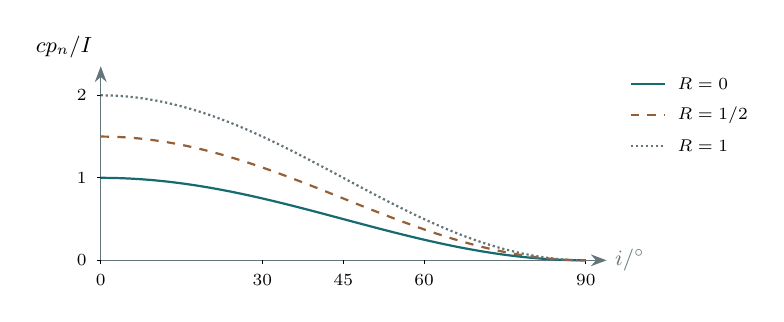
\begin{tikzpicture}[scale=.88,transform shape]
\draw[axis] (0,0.0)--(7.3,0.0) node[right] {$i/{}^\circ$};
\draw[axis] (0,0)--(0,2.8);
\node[above left] at (0,2.8) {$cp_n/I$};
\draw[thin] (0.000000,0.0)--(0.000000,-0.06);\node[below,font=\scriptsize] at (0.000000,-0.08) {$ 0 $};
\draw[thin] (2.333333,0.0)--(2.333333,-0.06);\node[below,font=\scriptsize] at (2.333333,-0.08) {$ 30 $};
\draw[thin] (3.500000,0.0)--(3.500000,-0.06);\node[below,font=\scriptsize] at (3.500000,-0.08) {$ 45 $};
\draw[thin] (4.666667,0.0)--(4.666667,-0.06);\node[below,font=\scriptsize] at (4.666667,-0.08) {$ 60 $};
\draw[thin] (7.000000,0.0)--(7.000000,-0.06);\node[below,font=\scriptsize] at (7.000000,-0.08) {$ 90 $};
\draw[thin] (0,0.000000)--(-.06,0.000000);\node[left,font=\scriptsize] at (-.08,0.000000) {$ 0 $};
\draw[thin] (0,1.190476)--(-.06,1.190476);\node[left,font=\scriptsize] at (-.08,1.190476) {$ 1 $};
\draw[thin] (0,2.380952)--(-.06,2.380952);\node[left,font=\scriptsize] at (-.08,2.380952) {$ 2 $};
\draw[thick,color=accent] plot coordinates {(0.0000000,1.1904762) (0.0291667,1.1904252) (0.0583333,1.1902722) (0.0875000,1.1900173) (0.1166667,1.1896604) (0.1458333,1.1892017) (0.1750000,1.1886413) (0.2041667,1.1879791) (0.2333333,1.1872154) (0.2625000,1.1863503) (0.2916667,1.1853838) (0.3208333,1.1843163) (0.3500000,1.1831478) (0.3791667,1.1818786) (0.4083333,1.1805089) (0.4375000,1.1790389) (0.4666667,1.1774688) (0.4958333,1.1757990) (0.5250000,1.1740297) (0.5541667,1.1721613) (0.5833333,1.1701939) (0.6125000,1.1681281) (0.6416667,1.1659641) (0.6708333,1.1637023) (0.7000000,1.1613432) (0.7291667,1.1588870) (0.7583333,1.1563342) (0.7875000,1.1536853) (0.8166667,1.1509407) (0.8458333,1.1481009) (0.8750000,1.1451664) (0.9041667,1.1421376) (0.9333333,1.1390152) (0.9625000,1.1357995) (0.9916667,1.1324912) (1.0208333,1.1290909) (1.0500000,1.1255991) (1.0791667,1.1220165) (1.1083333,1.1183435) (1.1375000,1.1145810) (1.1666667,1.1107294) (1.1958333,1.1067895) (1.2250000,1.1027620) (1.2541667,1.0986475) (1.2833333,1.0944468) (1.3125000,1.0901605) (1.3416667,1.0857894) (1.3708333,1.0813343) (1.4000000,1.0767958) (1.4291667,1.0721749) (1.4583333,1.0674722) (1.4875000,1.0626886) (1.5166667,1.0578250) (1.5458333,1.0528820) (1.5750000,1.0478607) (1.6041667,1.0427618) (1.6333333,1.0375862) (1.6625000,1.0323348) (1.6916667,1.0270086) (1.7208333,1.0216083) (1.7500000,1.0161350) (1.7791667,1.0105896) (1.8083333,1.0049730) (1.8375000,0.9992862) (1.8666667,0.9935301) (1.8958333,0.9877058) (1.9250000,0.9818143) (1.9541667,0.9758565) (1.9833333,0.9698336) (2.0125000,0.9637464) (2.0416667,0.9575961) (2.0708333,0.9513837) (2.1000000,0.9451103) (2.1291667,0.9387769) (2.1583333,0.9323847) (2.1875000,0.9259347) (2.2166667,0.9194280) (2.2458333,0.9128658) (2.2750000,0.9062491) (2.3041667,0.8995792) (2.3333333,0.8928571) (2.3625000,0.8860841) (2.3916667,0.8792612) (2.4208333,0.8723896) (2.4500000,0.8654705) (2.4791667,0.8585052) (2.5083333,0.8514947) (2.5375000,0.8444403) (2.5666667,0.8373432) (2.5958333,0.8302047) (2.6250000,0.8230259) (2.6541667,0.8158080) (2.6833333,0.8085524) (2.7125000,0.8012602) (2.7416667,0.7939327) (2.7708333,0.7865711) (2.8000000,0.7791768) (2.8291667,0.7717509) (2.8583333,0.7642948) (2.8875000,0.7568098) (2.9166667,0.7492971) (2.9458333,0.7417579) (2.9750000,0.7341937) (3.0041667,0.7266056) (3.0333333,0.7189951) (3.0625000,0.7113633) (3.0916667,0.7037116) (3.1208333,0.6960414) (3.1500000,0.6883538) (3.1791667,0.6806504) (3.2083333,0.6729323) (3.2375000,0.6652008) (3.2666667,0.6574574) (3.2958333,0.6497033) (3.3250000,0.6419399) (3.3541667,0.6341685) (3.3833333,0.6263905) (3.4125000,0.6186070) (3.4416667,0.6108196) (3.4708333,0.6030295) (3.5000000,0.5952381) (3.5291667,0.5874467) (3.5583333,0.5796566) (3.5875000,0.5718692) (3.6166667,0.5640857) (3.6458333,0.5563077) (3.6750000,0.5485363) (3.7041667,0.5407728) (3.7333333,0.5330188) (3.7625000,0.5252754) (3.7916667,0.5175439) (3.8208333,0.5098258) (3.8500000,0.5021223) (3.8791667,0.4944348) (3.9083333,0.4867646) (3.9375000,0.4791129) (3.9666667,0.4714811) (3.9958333,0.4638706) (4.0250000,0.4562825) (4.0541667,0.4487183) (4.0833333,0.4411791) (4.1125000,0.4336664) (4.1416667,0.4261813) (4.1708333,0.4187253) (4.2000000,0.4112994) (4.2291667,0.4039051) (4.2583333,0.3965435) (4.2875000,0.3892160) (4.3166667,0.3819238) (4.3458333,0.3746682) (4.3750000,0.3674503) (4.4041667,0.3602715) (4.4333333,0.3531330) (4.4625000,0.3460359) (4.4916667,0.3389815) (4.5208333,0.3319710) (4.5500000,0.3250057) (4.5791667,0.3180866) (4.6083333,0.3112150) (4.6375000,0.3043921) (4.6666667,0.2976190) (4.6958333,0.2908970) (4.7250000,0.2842270) (4.7541667,0.2776104) (4.7833333,0.2710482) (4.8125000,0.2645415) (4.8416667,0.2580915) (4.8708333,0.2516993) (4.9000000,0.2453659) (4.9291667,0.2390925) (4.9583333,0.2328801) (4.9875000,0.2267298) (5.0166667,0.2206426) (5.0458333,0.2146196) (5.0750000,0.2086619) (5.1041667,0.2027703) (5.1333333,0.1969461) (5.1625000,0.1911900) (5.1916667,0.1855032) (5.2208333,0.1798866) (5.2500000,0.1743412) (5.2791667,0.1688679) (5.3083333,0.1634676) (5.3375000,0.1581414) (5.3666667,0.1528900) (5.3958333,0.1477144) (5.4250000,0.1426155) (5.4541667,0.1375941) (5.4833333,0.1326512) (5.5125000,0.1277875) (5.5416667,0.1230040) (5.5708333,0.1183013) (5.6000000,0.1136804) (5.6291667,0.1091419) (5.6583333,0.1046868) (5.6875000,0.1003157) (5.7166667,0.0960294) (5.7458333,0.0918287) (5.7750000,0.0877142) (5.8041667,0.0836867) (5.8333333,0.0797468) (5.8625000,0.0758952) (5.8916667,0.0721327) (5.9208333,0.0684597) (5.9500000,0.0648771) (5.9791667,0.0613853) (6.0083333,0.0579849) (6.0375000,0.0546767) (6.0666667,0.0514610) (6.0958333,0.0483386) (6.1250000,0.0453098) (6.1541667,0.0423753) (6.1833333,0.0395355) (6.2125000,0.0367909) (6.2416667,0.0341420) (6.2708333,0.0315892) (6.3000000,0.0291330) (6.3291667,0.0267738) (6.3583333,0.0245121) (6.3875000,0.0223481) (6.4166667,0.0202822) (6.4458333,0.0183149) (6.4750000,0.0164465) (6.5041667,0.0146772) (6.5333333,0.0130074) (6.5625000,0.0114373) (6.5916667,0.0099673) (6.6208333,0.0085976) (6.6500000,0.0073284) (6.6791667,0.0061599) (6.7083333,0.0050923) (6.7375000,0.0041259) (6.7666667,0.0032608) (6.7958333,0.0024971) (6.8250000,0.0018349) (6.8541667,0.0012745) (6.8833333,0.0008158) (6.9125000,0.0004589) (6.9416667,0.0002040) (6.9708333,0.0000510) (7.0000000,0.0000000)};
\draw[thick,color=accent] (7.65,2.55)--(8.15,2.55);\node[right,font=\scriptsize] at (8.2,2.55) {$R=0$};
\draw[thick,dashed,color=warm] plot coordinates {(0.0000000,1.7857143) (0.0291667,1.7856378) (0.0583333,1.7854083) (0.0875000,1.7850259) (0.1166667,1.7844907) (0.1458333,1.7838026) (0.1750000,1.7829619) (0.2041667,1.7819687) (0.2333333,1.7808231) (0.2625000,1.7795254) (0.2916667,1.7780758) (0.3208333,1.7764745) (0.3500000,1.7747217) (0.3791667,1.7728179) (0.4083333,1.7707633) (0.4375000,1.7685583) (0.4666667,1.7662032) (0.4958333,1.7636985) (0.5250000,1.7610446) (0.5541667,1.7582419) (0.5833333,1.7552909) (0.6125000,1.7521922) (0.6416667,1.7489462) (0.6708333,1.7455535) (0.7000000,1.7420147) (0.7291667,1.7383305) (0.7583333,1.7345013) (0.7875000,1.7305280) (0.8166667,1.7264111) (0.8458333,1.7221514) (0.8750000,1.7177496) (0.9041667,1.7132064) (0.9333333,1.7085227) (0.9625000,1.7036993) (0.9916667,1.6987369) (1.0208333,1.6936364) (1.0500000,1.6883987) (1.0791667,1.6830247) (1.1083333,1.6775153) (1.1375000,1.6718714) (1.1666667,1.6660941) (1.1958333,1.6601843) (1.2250000,1.6541430) (1.2541667,1.6479713) (1.2833333,1.6416701) (1.3125000,1.6352407) (1.3416667,1.6286841) (1.3708333,1.6220014) (1.4000000,1.6151937) (1.4291667,1.6082623) (1.4583333,1.6012083) (1.4875000,1.5940330) (1.5166667,1.5867375) (1.5458333,1.5793231) (1.5750000,1.5717910) (1.6041667,1.5641427) (1.6333333,1.5563793) (1.6625000,1.5485022) (1.6916667,1.5405128) (1.7208333,1.5324124) (1.7500000,1.5242025) (1.7791667,1.5158843) (1.8083333,1.5074594) (1.8375000,1.4989292) (1.8666667,1.4902952) (1.8958333,1.4815588) (1.9250000,1.4727215) (1.9541667,1.4637848) (1.9833333,1.4547503) (2.0125000,1.4456196) (2.0416667,1.4363941) (2.0708333,1.4270755) (2.1000000,1.4176654) (2.1291667,1.4081653) (2.1583333,1.3985770) (2.1875000,1.3889020) (2.2166667,1.3791420) (2.2458333,1.3692987) (2.2750000,1.3593737) (2.3041667,1.3493688) (2.3333333,1.3392857) (2.3625000,1.3291261) (2.3916667,1.3188918) (2.4208333,1.3085844) (2.4500000,1.2982058) (2.4791667,1.2877578) (2.5083333,1.2772421) (2.5375000,1.2666605) (2.5666667,1.2560149) (2.5958333,1.2453070) (2.6250000,1.2345388) (2.6541667,1.2237120) (2.6833333,1.2128285) (2.7125000,1.2018902) (2.7416667,1.1908990) (2.7708333,1.1798567) (2.8000000,1.1687652) (2.8291667,1.1576264) (2.8583333,1.1464423) (2.8875000,1.1352147) (2.9166667,1.1239456) (2.9458333,1.1126369) (2.9750000,1.1012905) (3.0041667,1.0899084) (3.0333333,1.0784926) (3.0625000,1.0670449) (3.0916667,1.0555674) (3.1208333,1.0440621) (3.1500000,1.0325308) (3.1791667,1.0209756) (3.2083333,1.0093984) (3.2375000,0.9978012) (3.2666667,0.9861861) (3.2958333,0.9745550) (3.3250000,0.9629099) (3.3541667,0.9512528) (3.3833333,0.9395857) (3.4125000,0.9279105) (3.4416667,0.9162294) (3.4708333,0.9045443) (3.5000000,0.8928571) (3.5291667,0.8811700) (3.5583333,0.8694849) (3.5875000,0.8578037) (3.6166667,0.8461286) (3.6458333,0.8344615) (3.6750000,0.8228044) (3.7041667,0.8111593) (3.7333333,0.7995282) (3.7625000,0.7879130) (3.7916667,0.7763159) (3.8208333,0.7647387) (3.8500000,0.7531835) (3.8791667,0.7416522) (3.9083333,0.7301469) (3.9375000,0.7186694) (3.9666667,0.7072217) (3.9958333,0.6958059) (4.0250000,0.6844238) (4.0541667,0.6730774) (4.0833333,0.6617687) (4.1125000,0.6504996) (4.1416667,0.6392720) (4.1708333,0.6280879) (4.2000000,0.6169491) (4.2291667,0.6058576) (4.2583333,0.5948153) (4.2875000,0.5838241) (4.3166667,0.5728858) (4.3458333,0.5620023) (4.3750000,0.5511755) (4.4041667,0.5404073) (4.4333333,0.5296994) (4.4625000,0.5190538) (4.4916667,0.5084722) (4.5208333,0.4979565) (4.5500000,0.4875085) (4.5791667,0.4771299) (4.6083333,0.4668225) (4.6375000,0.4565882) (4.6666667,0.4464286) (4.6958333,0.4363455) (4.7250000,0.4263406) (4.7541667,0.4164156) (4.7833333,0.4065723) (4.8125000,0.3968123) (4.8416667,0.3871373) (4.8708333,0.3775489) (4.9000000,0.3680489) (4.9291667,0.3586387) (4.9583333,0.3493202) (4.9875000,0.3400947) (5.0166667,0.3309639) (5.0458333,0.3219295) (5.0750000,0.3129928) (5.1041667,0.3041555) (5.1333333,0.2954191) (5.1625000,0.2867850) (5.1916667,0.2782548) (5.2208333,0.2698299) (5.2500000,0.2615118) (5.2791667,0.2533018) (5.3083333,0.2452015) (5.3375000,0.2372120) (5.3666667,0.2293350) (5.3958333,0.2215716) (5.4250000,0.2139232) (5.4541667,0.2063912) (5.4833333,0.1989768) (5.5125000,0.1916813) (5.5416667,0.1845059) (5.5708333,0.1774520) (5.6000000,0.1705205) (5.6291667,0.1637129) (5.6583333,0.1570302) (5.6875000,0.1504736) (5.7166667,0.1440441) (5.7458333,0.1377430) (5.7750000,0.1315713) (5.8041667,0.1255300) (5.8333333,0.1196202) (5.8625000,0.1138429) (5.8916667,0.1081990) (5.9208333,0.1026896) (5.9500000,0.0973156) (5.9791667,0.0920779) (6.0083333,0.0869774) (6.0375000,0.0820150) (6.0666667,0.0771916) (6.0958333,0.0725078) (6.1250000,0.0679647) (6.1541667,0.0635629) (6.1833333,0.0593032) (6.2125000,0.0551863) (6.2416667,0.0512130) (6.2708333,0.0473838) (6.3000000,0.0436995) (6.3291667,0.0401608) (6.3583333,0.0367681) (6.3875000,0.0335221) (6.4166667,0.0304234) (6.4458333,0.0274724) (6.4750000,0.0246697) (6.5041667,0.0220158) (6.5333333,0.0195111) (6.5625000,0.0171560) (6.5916667,0.0149510) (6.6208333,0.0128964) (6.6500000,0.0109926) (6.6791667,0.0092398) (6.7083333,0.0076385) (6.7375000,0.0061889) (6.7666667,0.0048912) (6.7958333,0.0037456) (6.8250000,0.0027524) (6.8541667,0.0019117) (6.8833333,0.0012236) (6.9125000,0.0006884) (6.9416667,0.0003060) (6.9708333,0.0000765) (7.0000000,0.0000000)};
\draw[thick,dashed,color=warm] (7.65,2.0999999999999996)--(8.15,2.0999999999999996);\node[right,font=\scriptsize] at (8.2,2.0999999999999996) {$R=1/2$};
\draw[densely dotted,thick,color=muted] plot coordinates {(0.0000000,2.3809524) (0.0291667,2.3808504) (0.0583333,2.3805444) (0.0875000,2.3800346) (0.1166667,2.3793209) (0.1458333,2.3784035) (0.1750000,2.3772825) (0.2041667,2.3759582) (0.2333333,2.3744308) (0.2625000,2.3727005) (0.2916667,2.3707677) (0.3208333,2.3686326) (0.3500000,2.3662956) (0.3791667,2.3637572) (0.4083333,2.3610177) (0.4375000,2.3580777) (0.4666667,2.3549376) (0.4958333,2.3515980) (0.5250000,2.3480594) (0.5541667,2.3443225) (0.5833333,2.3403879) (0.6125000,2.3362562) (0.6416667,2.3319283) (0.6708333,2.3274047) (0.7000000,2.3226863) (0.7291667,2.3177740) (0.7583333,2.3126684) (0.7875000,2.3073706) (0.8166667,2.3018815) (0.8458333,2.2962018) (0.8750000,2.2903328) (0.9041667,2.2842753) (0.9333333,2.2780303) (0.9625000,2.2715990) (0.9916667,2.2649825) (1.0208333,2.2581818) (1.0500000,2.2511982) (1.0791667,2.2440329) (1.1083333,2.2366870) (1.1375000,2.2291619) (1.1666667,2.2214588) (1.1958333,2.2135791) (1.2250000,2.2055240) (1.2541667,2.1972950) (1.2833333,2.1888935) (1.3125000,2.1803210) (1.3416667,2.1715788) (1.3708333,2.1626685) (1.4000000,2.1535917) (1.4291667,2.1443498) (1.4583333,2.1349445) (1.4875000,2.1253773) (1.5166667,2.1156500) (1.5458333,2.1057641) (1.5750000,2.0957214) (1.6041667,2.0855236) (1.6333333,2.0751724) (1.6625000,2.0646697) (1.6916667,2.0540171) (1.7208333,2.0432166) (1.7500000,2.0322700) (1.7791667,2.0211791) (1.8083333,2.0099459) (1.8375000,1.9985723) (1.8666667,1.9870602) (1.8958333,1.9754117) (1.9250000,1.9636286) (1.9541667,1.9517131) (1.9833333,1.9396671) (2.0125000,1.9274928) (2.0416667,1.9151922) (2.0708333,1.9027674) (2.1000000,1.8902205) (2.1291667,1.8775538) (2.1583333,1.8647693) (2.1875000,1.8518693) (2.2166667,1.8388560) (2.2458333,1.8257316) (2.2750000,1.8124983) (2.3041667,1.7991584) (2.3333333,1.7857143) (2.3625000,1.7721681) (2.3916667,1.7585223) (2.4208333,1.7447792) (2.4500000,1.7309411) (2.4791667,1.7170103) (2.5083333,1.7029894) (2.5375000,1.6888806) (2.5666667,1.6746865) (2.5958333,1.6604094) (2.6250000,1.6460517) (2.6541667,1.6316160) (2.6833333,1.6171047) (2.7125000,1.6025203) (2.7416667,1.5878653) (2.7708333,1.5731422) (2.8000000,1.5583536) (2.8291667,1.5435019) (2.8583333,1.5285897) (2.8875000,1.5136196) (2.9166667,1.4985941) (2.9458333,1.4835158) (2.9750000,1.4683873) (3.0041667,1.4532112) (3.0333333,1.4379901) (3.0625000,1.4227266) (3.0916667,1.4074232) (3.1208333,1.3920827) (3.1500000,1.3767077) (3.1791667,1.3613007) (3.2083333,1.3458645) (3.2375000,1.3304017) (3.2666667,1.3149148) (3.2958333,1.2994067) (3.3250000,1.2838799) (3.3541667,1.2683371) (3.3833333,1.2527809) (3.4125000,1.2372141) (3.4416667,1.2216392) (3.4708333,1.2060590) (3.5000000,1.1904762) (3.5291667,1.1748933) (3.5583333,1.1593132) (3.5875000,1.1437383) (3.6166667,1.1281715) (3.6458333,1.1126153) (3.6750000,1.0970725) (3.7041667,1.0815457) (3.7333333,1.0660375) (3.7625000,1.0505507) (3.7916667,1.0350879) (3.8208333,1.0196516) (3.8500000,1.0042447) (3.8791667,0.9888696) (3.9083333,0.9735291) (3.9375000,0.9582258) (3.9666667,0.9429623) (3.9958333,0.9277411) (4.0250000,0.9125650) (4.0541667,0.8974366) (4.0833333,0.8823583) (4.1125000,0.8673328) (4.1416667,0.8523627) (4.1708333,0.8374505) (4.2000000,0.8225988) (4.2291667,0.8078102) (4.2583333,0.7930871) (4.2875000,0.7784321) (4.3166667,0.7638477) (4.3458333,0.7493364) (4.3750000,0.7349007) (4.4041667,0.7205430) (4.4333333,0.7062659) (4.4625000,0.6920717) (4.4916667,0.6779630) (4.5208333,0.6639420) (4.5500000,0.6500113) (4.5791667,0.6361732) (4.6083333,0.6224300) (4.6375000,0.6087842) (4.6666667,0.5952381) (4.6958333,0.5817939) (4.7250000,0.5684541) (4.7541667,0.5552208) (4.7833333,0.5420964) (4.8125000,0.5290831) (4.8416667,0.5161831) (4.8708333,0.5033986) (4.9000000,0.4907318) (4.9291667,0.4781850) (4.9583333,0.4657602) (4.9875000,0.4534596) (5.0166667,0.4412852) (5.0458333,0.4292393) (5.0750000,0.4173238) (5.1041667,0.4055407) (5.1333333,0.3938921) (5.1625000,0.3823801) (5.1916667,0.3710065) (5.2208333,0.3597733) (5.2500000,0.3486824) (5.2791667,0.3377358) (5.3083333,0.3269353) (5.3375000,0.3162827) (5.3666667,0.3057800) (5.3958333,0.2954288) (5.4250000,0.2852310) (5.4541667,0.2751883) (5.4833333,0.2653024) (5.5125000,0.2555751) (5.5416667,0.2460079) (5.5708333,0.2366026) (5.6000000,0.2273607) (5.6291667,0.2182839) (5.6583333,0.2093736) (5.6875000,0.2006314) (5.7166667,0.1920588) (5.7458333,0.1836574) (5.7750000,0.1754284) (5.8041667,0.1673733) (5.8333333,0.1594936) (5.8625000,0.1517905) (5.8916667,0.1442653) (5.9208333,0.1369195) (5.9500000,0.1297541) (5.9791667,0.1227705) (6.0083333,0.1159699) (6.0375000,0.1093534) (6.0666667,0.1029221) (6.0958333,0.0966771) (6.1250000,0.0906196) (6.1541667,0.0847505) (6.1833333,0.0790709) (6.2125000,0.0735817) (6.2416667,0.0682839) (6.2708333,0.0631784) (6.3000000,0.0582661) (6.3291667,0.0535477) (6.3583333,0.0490241) (6.3875000,0.0446961) (6.4166667,0.0405645) (6.4458333,0.0366299) (6.4750000,0.0328930) (6.5041667,0.0293544) (6.5333333,0.0260148) (6.5625000,0.0228747) (6.5916667,0.0199346) (6.6208333,0.0171952) (6.6500000,0.0146567) (6.6791667,0.0123198) (6.7083333,0.0101847) (6.7375000,0.0082518) (6.7666667,0.0065216) (6.7958333,0.0049941) (6.8250000,0.0036698) (6.8541667,0.0025489) (6.8833333,0.0016315) (6.9125000,0.0009178) (6.9416667,0.0004079) (6.9708333,0.0001020) (7.0000000,0.0000000)};
\draw[densely dotted,thick,color=muted] (7.65,1.65)--(8.15,1.65);\node[right,font=\scriptsize] at (8.2,1.65) {$R=1$};
\end{tikzpicture}
\figcaption{解图近1.1C\quad 镜面反射增强给表面的法向动量}
\end{minipage}\end{center}
\begin{center}\begin{minipage}{.98\linewidth}\centering
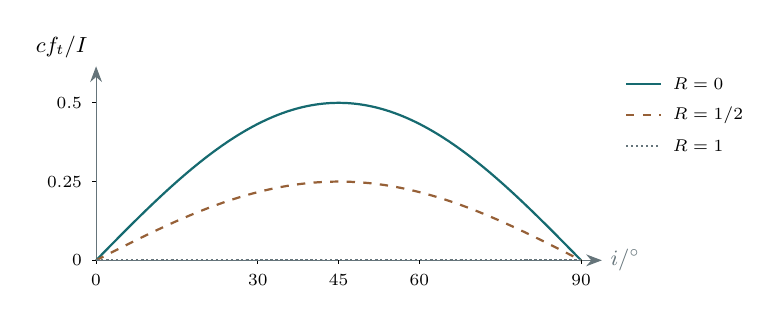
\begin{tikzpicture}[scale=.88,transform shape]
\draw[axis] (0,0.0)--(7.3,0.0) node[right] {$i/{}^\circ$};
\draw[axis] (0,0)--(0,2.8);
\node[above left] at (0,2.8) {$cf_t/I$};
\draw[thin] (0.000000,0.0)--(0.000000,-0.06);\node[below,font=\scriptsize] at (0.000000,-0.08) {$ 0 $};
\draw[thin] (2.333333,0.0)--(2.333333,-0.06);\node[below,font=\scriptsize] at (2.333333,-0.08) {$ 30 $};
\draw[thin] (3.500000,0.0)--(3.500000,-0.06);\node[below,font=\scriptsize] at (3.500000,-0.08) {$ 45 $};
\draw[thin] (4.666667,0.0)--(4.666667,-0.06);\node[below,font=\scriptsize] at (4.666667,-0.08) {$ 60 $};
\draw[thin] (7.000000,0.0)--(7.000000,-0.06);\node[below,font=\scriptsize] at (7.000000,-0.08) {$ 90 $};
\draw[thin] (0,0.000000)--(-.06,0.000000);\node[left,font=\scriptsize] at (-.08,0.000000) {$ 0 $};
\draw[thin] (0,1.136364)--(-.06,1.136364);\node[left,font=\scriptsize] at (-.08,1.136364) {$ 0.25 $};
\draw[thin] (0,2.272727)--(-.06,2.272727);\node[left,font=\scriptsize] at (-.08,2.272727) {$ 0.5 $};
\draw[thick,color=accent] plot coordinates {(0.0000000,0.0000000) (0.0291667,0.0297491) (0.0583333,0.0594931) (0.0875000,0.0892269) (0.1166667,0.1189454) (0.1458333,0.1486435) (0.1750000,0.1783161) (0.2041667,0.2079582) (0.2333333,0.2375647) (0.2625000,0.2671304) (0.2916667,0.2966504) (0.3208333,0.3261196) (0.3500000,0.3555329) (0.3791667,0.3848852) (0.4083333,0.4141716) (0.4375000,0.4433871) (0.4666667,0.4725266) (0.4958333,0.5015851) (0.5250000,0.5305576) (0.5541667,0.5594393) (0.5833333,0.5882251) (0.6125000,0.6169101) (0.6416667,0.6454894) (0.6708333,0.6739581) (0.7000000,0.7023114) (0.7291667,0.7305442) (0.7583333,0.7586520) (0.7875000,0.7866297) (0.8166667,0.8144726) (0.8458333,0.8421760) (0.8750000,0.8697351) (0.9041667,0.8971451) (0.9333333,0.9244015) (0.9625000,0.9514994) (0.9916667,0.9784343) (1.0208333,1.0052016) (1.0500000,1.0317966) (1.0791667,1.0582148) (1.1083333,1.0844517) (1.1375000,1.1105028) (1.1666667,1.1363636) (1.1958333,1.1620297) (1.2250000,1.1874967) (1.2541667,1.2127603) (1.2833333,1.2378160) (1.3125000,1.2626596) (1.3416667,1.2872869) (1.3708333,1.3116936) (1.4000000,1.3358756) (1.4291667,1.3598286) (1.4583333,1.3835487) (1.4875000,1.4070317) (1.5166667,1.4302736) (1.5458333,1.4532705) (1.5750000,1.4760183) (1.6041667,1.4985132) (1.6333333,1.5207514) (1.6625000,1.5427290) (1.6916667,1.5644422) (1.7208333,1.5858874) (1.7500000,1.6070609) (1.7791667,1.6279590) (1.8083333,1.6485781) (1.8375000,1.6689148) (1.8666667,1.6889655) (1.8958333,1.7087268) (1.9250000,1.7281954) (1.9541667,1.7473678) (1.9833333,1.7662408) (2.0125000,1.7848112) (2.0416667,1.8030758) (2.0708333,1.8210314) (2.1000000,1.8386750) (2.1291667,1.8560035) (2.1583333,1.8730141) (2.1875000,1.8897037) (2.2166667,1.9060695) (2.2458333,1.9221087) (2.2750000,1.9378186) (2.3041667,1.9531964) (2.3333333,1.9682396) (2.3625000,1.9829455) (2.3916667,1.9973116) (2.4208333,2.0113355) (2.4500000,2.0250148) (2.4791667,2.0383471) (2.5083333,2.0513302) (2.5375000,2.0639618) (2.5666667,2.0762397) (2.5958333,2.0881618) (2.6250000,2.0997262) (2.6541667,2.1109308) (2.6833333,2.1217737) (2.7125000,2.1322530) (2.7416667,2.1423670) (2.7708333,2.1521139) (2.8000000,2.1614921) (2.8291667,2.1704999) (2.8583333,2.1791358) (2.8875000,2.1873983) (2.9166667,2.1952860) (2.9458333,2.2027975) (2.9750000,2.2099316) (3.0041667,2.2166871) (3.0333333,2.2230627) (3.0625000,2.2290575) (3.0916667,2.2346702) (3.1208333,2.2399001) (3.1500000,2.2447462) (3.1791667,2.2492077) (3.2083333,2.2532838) (3.2375000,2.2569738) (3.2666667,2.2602770) (3.2958333,2.2631930) (3.3250000,2.2657212) (3.3541667,2.2678612) (3.3833333,2.2696126) (3.4125000,2.2709751) (3.4416667,2.2719485) (3.4708333,2.2725326) (3.5000000,2.2727273) (3.5291667,2.2725326) (3.5583333,2.2719485) (3.5875000,2.2709751) (3.6166667,2.2696126) (3.6458333,2.2678612) (3.6750000,2.2657212) (3.7041667,2.2631930) (3.7333333,2.2602770) (3.7625000,2.2569738) (3.7916667,2.2532838) (3.8208333,2.2492077) (3.8500000,2.2447462) (3.8791667,2.2399001) (3.9083333,2.2346702) (3.9375000,2.2290575) (3.9666667,2.2230627) (3.9958333,2.2166871) (4.0250000,2.2099316) (4.0541667,2.2027975) (4.0833333,2.1952860) (4.1125000,2.1873983) (4.1416667,2.1791358) (4.1708333,2.1704999) (4.2000000,2.1614921) (4.2291667,2.1521139) (4.2583333,2.1423670) (4.2875000,2.1322530) (4.3166667,2.1217737) (4.3458333,2.1109308) (4.3750000,2.0997262) (4.4041667,2.0881618) (4.4333333,2.0762397) (4.4625000,2.0639618) (4.4916667,2.0513302) (4.5208333,2.0383471) (4.5500000,2.0250148) (4.5791667,2.0113355) (4.6083333,1.9973116) (4.6375000,1.9829455) (4.6666667,1.9682396) (4.6958333,1.9531964) (4.7250000,1.9378186) (4.7541667,1.9221087) (4.7833333,1.9060695) (4.8125000,1.8897037) (4.8416667,1.8730141) (4.8708333,1.8560035) (4.9000000,1.8386750) (4.9291667,1.8210314) (4.9583333,1.8030758) (4.9875000,1.7848112) (5.0166667,1.7662408) (5.0458333,1.7473678) (5.0750000,1.7281954) (5.1041667,1.7087268) (5.1333333,1.6889655) (5.1625000,1.6689148) (5.1916667,1.6485781) (5.2208333,1.6279590) (5.2500000,1.6070609) (5.2791667,1.5858874) (5.3083333,1.5644422) (5.3375000,1.5427290) (5.3666667,1.5207514) (5.3958333,1.4985132) (5.4250000,1.4760183) (5.4541667,1.4532705) (5.4833333,1.4302736) (5.5125000,1.4070317) (5.5416667,1.3835487) (5.5708333,1.3598286) (5.6000000,1.3358756) (5.6291667,1.3116936) (5.6583333,1.2872869) (5.6875000,1.2626596) (5.7166667,1.2378160) (5.7458333,1.2127603) (5.7750000,1.1874967) (5.8041667,1.1620297) (5.8333333,1.1363636) (5.8625000,1.1105028) (5.8916667,1.0844517) (5.9208333,1.0582148) (5.9500000,1.0317966) (5.9791667,1.0052016) (6.0083333,0.9784343) (6.0375000,0.9514994) (6.0666667,0.9244015) (6.0958333,0.8971451) (6.1250000,0.8697351) (6.1541667,0.8421760) (6.1833333,0.8144726) (6.2125000,0.7866297) (6.2416667,0.7586520) (6.2708333,0.7305442) (6.3000000,0.7023114) (6.3291667,0.6739581) (6.3583333,0.6454894) (6.3875000,0.6169101) (6.4166667,0.5882251) (6.4458333,0.5594393) (6.4750000,0.5305576) (6.5041667,0.5015851) (6.5333333,0.4725266) (6.5625000,0.4433871) (6.5916667,0.4141716) (6.6208333,0.3848852) (6.6500000,0.3555329) (6.6791667,0.3261196) (6.7083333,0.2966504) (6.7375000,0.2671304) (6.7666667,0.2375647) (6.7958333,0.2079582) (6.8250000,0.1783161) (6.8541667,0.1486435) (6.8833333,0.1189454) (6.9125000,0.0892269) (6.9416667,0.0594931) (6.9708333,0.0297491) (7.0000000,0.0000000)};
\draw[thick,color=accent] (7.65,2.55)--(8.15,2.55);\node[right,font=\scriptsize] at (8.2,2.55) {$R=0$};
\draw[thick,dashed,color=warm] plot coordinates {(0.0000000,0.0000000) (0.0291667,0.0148745) (0.0583333,0.0297465) (0.0875000,0.0446134) (0.1166667,0.0594727) (0.1458333,0.0743217) (0.1750000,0.0891581) (0.2041667,0.1039791) (0.2333333,0.1187823) (0.2625000,0.1335652) (0.2916667,0.1483252) (0.3208333,0.1630598) (0.3500000,0.1777664) (0.3791667,0.1924426) (0.4083333,0.2070858) (0.4375000,0.2216935) (0.4666667,0.2362633) (0.4958333,0.2507925) (0.5250000,0.2652788) (0.5541667,0.2797197) (0.5833333,0.2941126) (0.6125000,0.3084551) (0.6416667,0.3227447) (0.6708333,0.3369791) (0.7000000,0.3511557) (0.7291667,0.3652721) (0.7583333,0.3793260) (0.7875000,0.3933148) (0.8166667,0.4072363) (0.8458333,0.4210880) (0.8750000,0.4348675) (0.9041667,0.4485726) (0.9333333,0.4622007) (0.9625000,0.4757497) (0.9916667,0.4892172) (1.0208333,0.5026008) (1.0500000,0.5158983) (1.0791667,0.5291074) (1.1083333,0.5422259) (1.1375000,0.5552514) (1.1666667,0.5681818) (1.1958333,0.5810149) (1.2250000,0.5937484) (1.2541667,0.6063801) (1.2833333,0.6189080) (1.3125000,0.6313298) (1.3416667,0.6436435) (1.3708333,0.6558468) (1.4000000,0.6679378) (1.4291667,0.6799143) (1.4583333,0.6917744) (1.4875000,0.7035159) (1.5166667,0.7151368) (1.5458333,0.7266352) (1.5750000,0.7380091) (1.6041667,0.7492566) (1.6333333,0.7603757) (1.6625000,0.7713645) (1.6916667,0.7822211) (1.7208333,0.7929437) (1.7500000,0.8035304) (1.7791667,0.8139795) (1.8083333,0.8242891) (1.8375000,0.8344574) (1.8666667,0.8444828) (1.8958333,0.8543634) (1.9250000,0.8640977) (1.9541667,0.8736839) (1.9833333,0.8831204) (2.0125000,0.8924056) (2.0416667,0.9015379) (2.0708333,0.9105157) (2.1000000,0.9193375) (2.1291667,0.9280018) (2.1583333,0.9365070) (2.1875000,0.9448518) (2.2166667,0.9530347) (2.2458333,0.9610543) (2.2750000,0.9689093) (2.3041667,0.9765982) (2.3333333,0.9841198) (2.3625000,0.9914727) (2.3916667,0.9986558) (2.4208333,1.0056678) (2.4500000,1.0125074) (2.4791667,1.0191736) (2.5083333,1.0256651) (2.5375000,1.0319809) (2.5666667,1.0381198) (2.5958333,1.0440809) (2.6250000,1.0498631) (2.6541667,1.0554654) (2.6833333,1.0608868) (2.7125000,1.0661265) (2.7416667,1.0711835) (2.7708333,1.0760570) (2.8000000,1.0807460) (2.8291667,1.0852499) (2.8583333,1.0895679) (2.8875000,1.0936991) (2.9166667,1.0976430) (2.9458333,1.1013988) (2.9750000,1.1049658) (3.0041667,1.1083435) (3.0333333,1.1115314) (3.0625000,1.1145287) (3.0916667,1.1173351) (3.1208333,1.1199501) (3.1500000,1.1223731) (3.1791667,1.1246038) (3.2083333,1.1266419) (3.2375000,1.1284869) (3.2666667,1.1301385) (3.2958333,1.1315965) (3.3250000,1.1328606) (3.3541667,1.1339306) (3.3833333,1.1348063) (3.4125000,1.1354875) (3.4416667,1.1359742) (3.4708333,1.1362663) (3.5000000,1.1363636) (3.5291667,1.1362663) (3.5583333,1.1359742) (3.5875000,1.1354875) (3.6166667,1.1348063) (3.6458333,1.1339306) (3.6750000,1.1328606) (3.7041667,1.1315965) (3.7333333,1.1301385) (3.7625000,1.1284869) (3.7916667,1.1266419) (3.8208333,1.1246038) (3.8500000,1.1223731) (3.8791667,1.1199501) (3.9083333,1.1173351) (3.9375000,1.1145287) (3.9666667,1.1115314) (3.9958333,1.1083435) (4.0250000,1.1049658) (4.0541667,1.1013988) (4.0833333,1.0976430) (4.1125000,1.0936991) (4.1416667,1.0895679) (4.1708333,1.0852499) (4.2000000,1.0807460) (4.2291667,1.0760570) (4.2583333,1.0711835) (4.2875000,1.0661265) (4.3166667,1.0608868) (4.3458333,1.0554654) (4.3750000,1.0498631) (4.4041667,1.0440809) (4.4333333,1.0381198) (4.4625000,1.0319809) (4.4916667,1.0256651) (4.5208333,1.0191736) (4.5500000,1.0125074) (4.5791667,1.0056678) (4.6083333,0.9986558) (4.6375000,0.9914727) (4.6666667,0.9841198) (4.6958333,0.9765982) (4.7250000,0.9689093) (4.7541667,0.9610543) (4.7833333,0.9530347) (4.8125000,0.9448518) (4.8416667,0.9365070) (4.8708333,0.9280018) (4.9000000,0.9193375) (4.9291667,0.9105157) (4.9583333,0.9015379) (4.9875000,0.8924056) (5.0166667,0.8831204) (5.0458333,0.8736839) (5.0750000,0.8640977) (5.1041667,0.8543634) (5.1333333,0.8444828) (5.1625000,0.8344574) (5.1916667,0.8242891) (5.2208333,0.8139795) (5.2500000,0.8035304) (5.2791667,0.7929437) (5.3083333,0.7822211) (5.3375000,0.7713645) (5.3666667,0.7603757) (5.3958333,0.7492566) (5.4250000,0.7380091) (5.4541667,0.7266352) (5.4833333,0.7151368) (5.5125000,0.7035159) (5.5416667,0.6917744) (5.5708333,0.6799143) (5.6000000,0.6679378) (5.6291667,0.6558468) (5.6583333,0.6436435) (5.6875000,0.6313298) (5.7166667,0.6189080) (5.7458333,0.6063801) (5.7750000,0.5937484) (5.8041667,0.5810149) (5.8333333,0.5681818) (5.8625000,0.5552514) (5.8916667,0.5422259) (5.9208333,0.5291074) (5.9500000,0.5158983) (5.9791667,0.5026008) (6.0083333,0.4892172) (6.0375000,0.4757497) (6.0666667,0.4622007) (6.0958333,0.4485726) (6.1250000,0.4348675) (6.1541667,0.4210880) (6.1833333,0.4072363) (6.2125000,0.3933148) (6.2416667,0.3793260) (6.2708333,0.3652721) (6.3000000,0.3511557) (6.3291667,0.3369791) (6.3583333,0.3227447) (6.3875000,0.3084551) (6.4166667,0.2941126) (6.4458333,0.2797197) (6.4750000,0.2652788) (6.5041667,0.2507925) (6.5333333,0.2362633) (6.5625000,0.2216935) (6.5916667,0.2070858) (6.6208333,0.1924426) (6.6500000,0.1777664) (6.6791667,0.1630598) (6.7083333,0.1483252) (6.7375000,0.1335652) (6.7666667,0.1187823) (6.7958333,0.1039791) (6.8250000,0.0891581) (6.8541667,0.0743217) (6.8833333,0.0594727) (6.9125000,0.0446134) (6.9416667,0.0297465) (6.9708333,0.0148745) (7.0000000,0.0000000)};
\draw[thick,dashed,color=warm] (7.65,2.0999999999999996)--(8.15,2.0999999999999996);\node[right,font=\scriptsize] at (8.2,2.0999999999999996) {$R=1/2$};
\draw[densely dotted,thick,color=muted] plot coordinates {(0.0000000,0.0000000) (0.0291667,0.0000000) (0.0583333,0.0000000) (0.0875000,0.0000000) (0.1166667,0.0000000) (0.1458333,0.0000000) (0.1750000,0.0000000) (0.2041667,0.0000000) (0.2333333,0.0000000) (0.2625000,0.0000000) (0.2916667,0.0000000) (0.3208333,0.0000000) (0.3500000,0.0000000) (0.3791667,0.0000000) (0.4083333,0.0000000) (0.4375000,0.0000000) (0.4666667,0.0000000) (0.4958333,0.0000000) (0.5250000,0.0000000) (0.5541667,0.0000000) (0.5833333,0.0000000) (0.6125000,0.0000000) (0.6416667,0.0000000) (0.6708333,0.0000000) (0.7000000,0.0000000) (0.7291667,0.0000000) (0.7583333,0.0000000) (0.7875000,0.0000000) (0.8166667,0.0000000) (0.8458333,0.0000000) (0.8750000,0.0000000) (0.9041667,0.0000000) (0.9333333,0.0000000) (0.9625000,0.0000000) (0.9916667,0.0000000) (1.0208333,0.0000000) (1.0500000,0.0000000) (1.0791667,0.0000000) (1.1083333,0.0000000) (1.1375000,0.0000000) (1.1666667,0.0000000) (1.1958333,0.0000000) (1.2250000,0.0000000) (1.2541667,0.0000000) (1.2833333,0.0000000) (1.3125000,0.0000000) (1.3416667,0.0000000) (1.3708333,0.0000000) (1.4000000,0.0000000) (1.4291667,0.0000000) (1.4583333,0.0000000) (1.4875000,0.0000000) (1.5166667,0.0000000) (1.5458333,0.0000000) (1.5750000,0.0000000) (1.6041667,0.0000000) (1.6333333,0.0000000) (1.6625000,0.0000000) (1.6916667,0.0000000) (1.7208333,0.0000000) (1.7500000,0.0000000) (1.7791667,0.0000000) (1.8083333,0.0000000) (1.8375000,0.0000000) (1.8666667,0.0000000) (1.8958333,0.0000000) (1.9250000,0.0000000) (1.9541667,0.0000000) (1.9833333,0.0000000) (2.0125000,0.0000000) (2.0416667,0.0000000) (2.0708333,0.0000000) (2.1000000,0.0000000) (2.1291667,0.0000000) (2.1583333,0.0000000) (2.1875000,0.0000000) (2.2166667,0.0000000) (2.2458333,0.0000000) (2.2750000,0.0000000) (2.3041667,0.0000000) (2.3333333,0.0000000) (2.3625000,0.0000000) (2.3916667,0.0000000) (2.4208333,0.0000000) (2.4500000,0.0000000) (2.4791667,0.0000000) (2.5083333,0.0000000) (2.5375000,0.0000000) (2.5666667,0.0000000) (2.5958333,0.0000000) (2.6250000,0.0000000) (2.6541667,0.0000000) (2.6833333,0.0000000) (2.7125000,0.0000000) (2.7416667,0.0000000) (2.7708333,0.0000000) (2.8000000,0.0000000) (2.8291667,0.0000000) (2.8583333,0.0000000) (2.8875000,0.0000000) (2.9166667,0.0000000) (2.9458333,0.0000000) (2.9750000,0.0000000) (3.0041667,0.0000000) (3.0333333,0.0000000) (3.0625000,0.0000000) (3.0916667,0.0000000) (3.1208333,0.0000000) (3.1500000,0.0000000) (3.1791667,0.0000000) (3.2083333,0.0000000) (3.2375000,0.0000000) (3.2666667,0.0000000) (3.2958333,0.0000000) (3.3250000,0.0000000) (3.3541667,0.0000000) (3.3833333,0.0000000) (3.4125000,0.0000000) (3.4416667,0.0000000) (3.4708333,0.0000000) (3.5000000,0.0000000) (3.5291667,0.0000000) (3.5583333,0.0000000) (3.5875000,0.0000000) (3.6166667,0.0000000) (3.6458333,0.0000000) (3.6750000,0.0000000) (3.7041667,0.0000000) (3.7333333,0.0000000) (3.7625000,0.0000000) (3.7916667,0.0000000) (3.8208333,0.0000000) (3.8500000,0.0000000) (3.8791667,0.0000000) (3.9083333,0.0000000) (3.9375000,0.0000000) (3.9666667,0.0000000) (3.9958333,0.0000000) (4.0250000,0.0000000) (4.0541667,0.0000000) (4.0833333,0.0000000) (4.1125000,0.0000000) (4.1416667,0.0000000) (4.1708333,0.0000000) (4.2000000,0.0000000) (4.2291667,0.0000000) (4.2583333,0.0000000) (4.2875000,0.0000000) (4.3166667,0.0000000) (4.3458333,0.0000000) (4.3750000,0.0000000) (4.4041667,0.0000000) (4.4333333,0.0000000) (4.4625000,0.0000000) (4.4916667,0.0000000) (4.5208333,0.0000000) (4.5500000,0.0000000) (4.5791667,0.0000000) (4.6083333,0.0000000) (4.6375000,0.0000000) (4.6666667,0.0000000) (4.6958333,0.0000000) (4.7250000,0.0000000) (4.7541667,0.0000000) (4.7833333,0.0000000) (4.8125000,0.0000000) (4.8416667,0.0000000) (4.8708333,0.0000000) (4.9000000,0.0000000) (4.9291667,0.0000000) (4.9583333,0.0000000) (4.9875000,0.0000000) (5.0166667,0.0000000) (5.0458333,0.0000000) (5.0750000,0.0000000) (5.1041667,0.0000000) (5.1333333,0.0000000) (5.1625000,0.0000000) (5.1916667,0.0000000) (5.2208333,0.0000000) (5.2500000,0.0000000) (5.2791667,0.0000000) (5.3083333,0.0000000) (5.3375000,0.0000000) (5.3666667,0.0000000) (5.3958333,0.0000000) (5.4250000,0.0000000) (5.4541667,0.0000000) (5.4833333,0.0000000) (5.5125000,0.0000000) (5.5416667,0.0000000) (5.5708333,0.0000000) (5.6000000,0.0000000) (5.6291667,0.0000000) (5.6583333,0.0000000) (5.6875000,0.0000000) (5.7166667,0.0000000) (5.7458333,0.0000000) (5.7750000,0.0000000) (5.8041667,0.0000000) (5.8333333,0.0000000) (5.8625000,0.0000000) (5.8916667,0.0000000) (5.9208333,0.0000000) (5.9500000,0.0000000) (5.9791667,0.0000000) (6.0083333,0.0000000) (6.0375000,0.0000000) (6.0666667,0.0000000) (6.0958333,0.0000000) (6.1250000,0.0000000) (6.1541667,0.0000000) (6.1833333,0.0000000) (6.2125000,0.0000000) (6.2416667,0.0000000) (6.2708333,0.0000000) (6.3000000,0.0000000) (6.3291667,0.0000000) (6.3583333,0.0000000) (6.3875000,0.0000000) (6.4166667,0.0000000) (6.4458333,0.0000000) (6.4750000,0.0000000) (6.5041667,0.0000000) (6.5333333,0.0000000) (6.5625000,0.0000000) (6.5916667,0.0000000) (6.6208333,0.0000000) (6.6500000,0.0000000) (6.6791667,0.0000000) (6.7083333,0.0000000) (6.7375000,0.0000000) (6.7666667,0.0000000) (6.7958333,0.0000000) (6.8250000,0.0000000) (6.8541667,0.0000000) (6.8833333,0.0000000) (6.9125000,0.0000000) (6.9416667,0.0000000) (6.9708333,0.0000000) (7.0000000,0.0000000)};
\draw[densely dotted,thick,color=muted] (7.65,1.65)--(8.15,1.65);\node[right,font=\scriptsize] at (8.2,1.65) {$R=1$};
\end{tikzpicture}
\figcaption{解图近1.1D\quad 切向转移由吸收事件留下，在45度达到最大}
\end{minipage}\end{center}
若另给的是单位实际表面积收到的功率密度$J=I\cos i$，公式可写$p_n=(1+R)J\cos i/c$、$f_t=(1-R)J\sin i/c$，面积投影已包含在$J$的定义中。两种强度定义使用同一命中功率，保持单位与实际受照面积对应。

正入射时$p_n=(1+R)I/c$、$f_t=0$。完全反射时每个光子的切向动量保持，故$f_t=0$、$p_n=2I\cos^2i/c$；完全吸收时力沿入射方向，$f_t/p_n=\tan i$。固定光束强度$I$时，掠入射极限$\cos i\to0$使同一实际表面截获功率趋零，两种力密度均趋零。完全吸收的两分量合成为$(I\cos i/c)\hat{\boldsymbol k}_i$，也与“吸收功率除以$c$”相符。

上述反射方向由镜面关系确定。若给出反射光的归一化出射分布$w(\Omega)$，则平均方向为$\langle\hat{\boldsymbol k}_{\rm out}\rangle=\int w(\Omega)\hat{\boldsymbol k}_{\rm out}\,\dd\Omega$，同一动量通量式写成$\boldsymbol f=J[\hat{\boldsymbol k}_i-R\langle\hat{\boldsymbol k}_{\rm out}\rangle]/c$。镜面反射的分布集中在$\hat{\boldsymbol k}_r$，便回到前面所得矢量式；角分布改变时，按实际出射平均求反冲。


\Needspace{8\baselineskip}

\pdfbookmark[3]{关键洞察}{q1-h5}

\subsection*{关键洞察}

镜面反射的光子带有切向动量，反射后该分量仍相同，所以这类事件的切向转移为零。压力中的两个余弦分别描述命中数量和法向动量，改变强度定义时相应把面积因子并入$J$。

\Needspace{8\baselineskip}

\pdfbookmark[3]{易错点}{q1-h6}

\subsection*{易错点}

\begin{itemize}
\item 命中功率为$I\dd S\cos i$，按光束垂直截面计数。
\item 表面收到的冲量是光子初动量减末动量，与光子自身的动量变化相反。
\item 镜面出射使用单一反射方向，漫反射使用角分布加权的出射动量。
\item 固定$I$与固定$J$对应不同受控照明条件，各自从实际截获功率求力。
\end{itemize}

\Needspace{8\baselineskip}

\pdfbookmark[3]{课堂讲解建议}{q1-h7}

\subsection*{课堂讲解建议}

先画一个反射光子的入射、出射动量箭头，让学生沿法线和切线分别作差，再把单事件扩大为光子流。用60度完全反射和正入射比较压力，面积投影与单光子法向投影各减半，总结果为四分之一。接着改为完全吸收，由矢量合成指出合力沿光束。最后讨论固定实际面功率密度以及Lambert出射，用改变的具体量重新写动量通量。

\Needspace{8\baselineskip}

\pdfbookmark[3]{变式训练}{q1-h8}

\subsection*{变式训练}

\begin{enumerate}
\item \textbf{半反射表面的45度入射。}取$i=45^\circ,R=1/2$，求力的两个分量和合力偏离内法线的角度。

由两种投影，$p_n=(I/c)(3/2)(1/2)=3I/(4c)$，$f_t=(I/c)(1/2)(1/2)=I/(4c)$。故$\tan\psi=f_t/p_n=1/3$，$\psi=\arctan(1/3)=18.4349^\circ$。变图近1.1V1画法向、切向和合力的矢量三角形，合力大小为$\sqrt{10}I/(4c)$。
\begin{center}\begin{minipage}{.98\linewidth}\centering
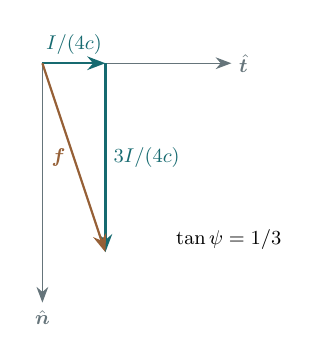
\begin{tikzpicture}[scale=.8,transform shape]
\draw[axis] (0,0)--(3,0) node[right] {$\hat{\boldsymbol t}$};
\draw[axis] (0,0)--(0,-3.8) node[below] {$\hat{\boldsymbol n}$};
\draw[motion] (0,0)--(1,0) node[midway,above] {$I/(4c)$};
\draw[motion] (1,0)--(1,-3) node[midway,right] {$3I/(4c)$};
\draw[force] (0,0)--(1,-3) node[midway,left] {$\boldsymbol f$};
\node[right] at (2,-2.8) {$\tan\psi=1/3$};
\end{tikzpicture}
\figcaption{变图近1.1V1\quad 45度半反射表面的合力三角形}
\end{minipage}\end{center}
\item \textbf{以实际面上功率密度为已知量。}现在固定$J=I\cos i$，求反射率$R=1/2$时随入射角变化的两力密度。

把$I\cos i$整体换成$J$，得到
\[
 p_n=\frac{3J}{2c}\cos i,\qquad f_t=\frac{J}{2c}\sin i.
\]
变图近1.1V2画按$J/c$归一化的分量。接近掠入射还保持$J$，意味着照明的光束垂直强度$I=J/\cos i$同步增大；这组受控条件与固定$I$的主解分别对应其实际截获功率。
\begin{center}\begin{minipage}{.98\linewidth}\centering
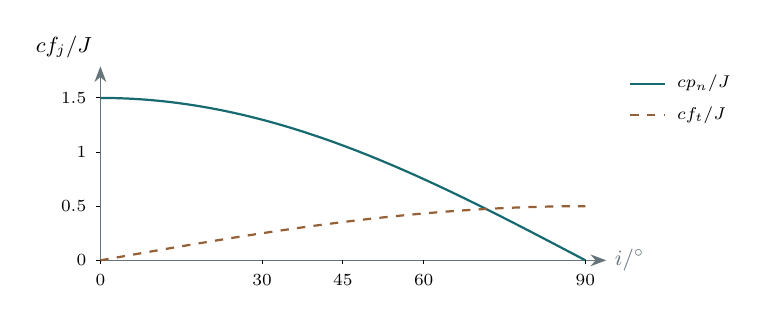
\begin{tikzpicture}[scale=.88,transform shape]
\draw[axis] (0,0.0)--(7.3,0.0) node[right] {$i/{}^\circ$};
\draw[axis] (0,0)--(0,2.8);
\node[above left] at (0,2.8) {$cf_j/J$};
\draw[thin] (0.000000,0.0)--(0.000000,-0.06);\node[below,font=\scriptsize] at (0.000000,-0.08) {$ 0 $};
\draw[thin] (2.333333,0.0)--(2.333333,-0.06);\node[below,font=\scriptsize] at (2.333333,-0.08) {$ 30 $};
\draw[thin] (3.500000,0.0)--(3.500000,-0.06);\node[below,font=\scriptsize] at (3.500000,-0.08) {$ 45 $};
\draw[thin] (4.666667,0.0)--(4.666667,-0.06);\node[below,font=\scriptsize] at (4.666667,-0.08) {$ 60 $};
\draw[thin] (7.000000,0.0)--(7.000000,-0.06);\node[below,font=\scriptsize] at (7.000000,-0.08) {$ 90 $};
\draw[thin] (0,0.000000)--(-.06,0.000000);\node[left,font=\scriptsize] at (-.08,0.000000) {$ 0 $};
\draw[thin] (0,0.781250)--(-.06,0.781250);\node[left,font=\scriptsize] at (-.08,0.781250) {$ 0.5 $};
\draw[thin] (0,1.562500)--(-.06,1.562500);\node[left,font=\scriptsize] at (-.08,1.562500) {$ 1 $};
\draw[thin] (0,2.343750)--(-.06,2.343750);\node[left,font=\scriptsize] at (-.08,2.343750) {$ 1.5 $};
\draw[thick,color=accent] plot coordinates {(0.0000000,2.3437500) (0.0291667,2.3436998) (0.0583333,2.3435492) (0.0875000,2.3432982) (0.1166667,2.3429469) (0.1458333,2.3424951) (0.1750000,2.3419431) (0.2041667,2.3412907) (0.2333333,2.3405380) (0.2625000,2.3396850) (0.2916667,2.3387319) (0.3208333,2.3376785) (0.3500000,2.3365250) (0.3791667,2.3352714) (0.4083333,2.3339178) (0.4375000,2.3324642) (0.4666667,2.3309107) (0.4958333,2.3292573) (0.5250000,2.3275042) (0.5541667,2.3256514) (0.5833333,2.3236989) (0.6125000,2.3216469) (0.6416667,2.3194954) (0.6708333,2.3172446) (0.7000000,2.3148945) (0.7291667,2.3124453) (0.7583333,2.3098970) (0.7875000,2.3072498) (0.8166667,2.3045037) (0.8458333,2.3016589) (0.8750000,2.2987155) (0.9041667,2.2956736) (0.9333333,2.2925334) (0.9625000,2.2892950) (0.9916667,2.2859586) (1.0208333,2.2825242) (1.0500000,2.2789920) (1.0791667,2.2753622) (1.1083333,2.2716349) (1.1375000,2.2678104) (1.1666667,2.2638887) (1.1958333,2.2598700) (1.2250000,2.2557545) (1.2541667,2.2515423) (1.2833333,2.2472338) (1.3125000,2.2428289) (1.3416667,2.2383280) (1.3708333,2.2337312) (1.4000000,2.2290387) (1.4291667,2.2242507) (1.4583333,2.2193675) (1.4875000,2.2143892) (1.5166667,2.2093160) (1.5458333,2.2041482) (1.5750000,2.1988859) (1.6041667,2.1935295) (1.6333333,2.1880791) (1.6625000,2.1825350) (1.6916667,2.1768974) (1.7208333,2.1711665) (1.7500000,2.1653427) (1.7791667,2.1594260) (1.8083333,2.1534169) (1.8375000,2.1473155) (1.8666667,2.1411222) (1.8958333,2.1348371) (1.9250000,2.1284606) (1.9541667,2.1219929) (1.9833333,2.1154343) (2.0125000,2.1087850) (2.0416667,2.1020455) (2.0708333,2.0952159) (2.1000000,2.0882965) (2.1291667,2.0812877) (2.1583333,2.0741898) (2.1875000,2.0670030) (2.2166667,2.0597276) (2.2458333,2.0523640) (2.2750000,2.0449125) (2.3041667,2.0373734) (2.3333333,2.0297470) (2.3625000,2.0220337) (2.3916667,2.0142338) (2.4208333,2.0063476) (2.4500000,1.9983754) (2.4791667,1.9903176) (2.5083333,1.9821746) (2.5375000,1.9739466) (2.5666667,1.9656341) (2.5958333,1.9572374) (2.6250000,1.9487569) (2.6541667,1.9401929) (2.6833333,1.9315458) (2.7125000,1.9228159) (2.7416667,1.9140036) (2.7708333,1.9051094) (2.8000000,1.8961336) (2.8291667,1.8870765) (2.8583333,1.8779386) (2.8875000,1.8687203) (2.9166667,1.8594219) (2.9458333,1.8500438) (2.9750000,1.8405866) (3.0041667,1.8310504) (3.0333333,1.8214358) (3.0625000,1.8117433) (3.0916667,1.8019730) (3.1208333,1.7921256) (3.1500000,1.7822015) (3.1791667,1.7722010) (3.2083333,1.7621245) (3.2375000,1.7519726) (3.2666667,1.7417457) (3.2958333,1.7314441) (3.3250000,1.7210684) (3.3541667,1.7106189) (3.3833333,1.7000962) (3.4125000,1.6895006) (3.4416667,1.6788327) (3.4708333,1.6680928) (3.5000000,1.6572815) (3.5291667,1.6463992) (3.5583333,1.6354464) (3.5875000,1.6244235) (3.6166667,1.6133310) (3.6458333,1.6021695) (3.6750000,1.5909392) (3.7041667,1.5796409) (3.7333333,1.5682749) (3.7625000,1.5568417) (3.7916667,1.5453418) (3.8208333,1.5337757) (3.8500000,1.5221439) (3.8791667,1.5104469) (3.9083333,1.4986852) (3.9375000,1.4868593) (3.9666667,1.4749697) (3.9958333,1.4630169) (4.0250000,1.4510014) (4.0541667,1.4389238) (4.0833333,1.4267846) (4.1125000,1.4145842) (4.1416667,1.4023233) (4.1708333,1.3900023) (4.2000000,1.3776217) (4.2291667,1.3651821) (4.2583333,1.3526840) (4.2875000,1.3401280) (4.3166667,1.3275146) (4.3458333,1.3148443) (4.3750000,1.3021177) (4.4041667,1.2893354) (4.4333333,1.2764977) (4.4625000,1.2636054) (4.4916667,1.2506590) (4.5208333,1.2376590) (4.5500000,1.2246060) (4.5791667,1.2115005) (4.6083333,1.1983432) (4.6375000,1.1851345) (4.6666667,1.1718750) (4.6958333,1.1585653) (4.7250000,1.1452060) (4.7541667,1.1317977) (4.7833333,1.1183408) (4.8125000,1.1048361) (4.8416667,1.0912840) (4.8708333,1.0776852) (4.9000000,1.0640402) (4.9291667,1.0503497) (4.9583333,1.0366141) (4.9875000,1.0228342) (5.0166667,1.0090104) (5.0458333,0.9951434) (5.0750000,0.9812338) (5.1041667,0.9672821) (5.1333333,0.9532890) (5.1625000,0.9392551) (5.1916667,0.9251809) (5.2208333,0.9110671) (5.2500000,0.8969143) (5.2791667,0.8827231) (5.3083333,0.8684940) (5.3375000,0.8542277) (5.3666667,0.8399249) (5.3958333,0.8255860) (5.4250000,0.8112119) (5.4541667,0.7968029) (5.4833333,0.7823598) (5.5125000,0.7678832) (5.5416667,0.7533737) (5.5708333,0.7388320) (5.6000000,0.7242586) (5.6291667,0.7096541) (5.6583333,0.6950193) (5.6875000,0.6803547) (5.7166667,0.6656610) (5.7458333,0.6509387) (5.7750000,0.6361886) (5.8041667,0.6214112) (5.8333333,0.6066071) (5.8625000,0.5917771) (5.8916667,0.5769218) (5.9208333,0.5620417) (5.9500000,0.5471376) (5.9791667,0.5322100) (6.0083333,0.5172596) (6.0375000,0.5022871) (6.0666667,0.4872930) (6.0958333,0.4722781) (6.1250000,0.4572429) (6.1541667,0.4421882) (6.1833333,0.4271145) (6.2125000,0.4120225) (6.2416667,0.3969129) (6.2708333,0.3817863) (6.3000000,0.3666433) (6.3291667,0.3514846) (6.3583333,0.3363108) (6.3875000,0.3211227) (6.4166667,0.3059208) (6.4458333,0.2907057) (6.4750000,0.2754783) (6.5041667,0.2602390) (6.5333333,0.2449886) (6.5625000,0.2297277) (6.5916667,0.2144569) (6.6208333,0.1991770) (6.6500000,0.1838885) (6.6791667,0.1685922) (6.7083333,0.1532886) (6.7375000,0.1379784) (6.7666667,0.1226624) (6.7958333,0.1073411) (6.8250000,0.0920152) (6.8541667,0.0766854) (6.8833333,0.0613522) (6.9125000,0.0460165) (6.9416667,0.0306787) (6.9708333,0.0153397) (7.0000000,0.0000000)};
\draw[thick,color=accent] (7.65,2.55)--(8.15,2.55);\node[right,font=\scriptsize] at (8.2,2.55) {$cp_n/J$};
\draw[thick,dashed,color=warm] plot coordinates {(0.0000000,0.0000000) (0.0291667,0.0051132) (0.0583333,0.0102262) (0.0875000,0.0153388) (0.1166667,0.0204507) (0.1458333,0.0255618) (0.1750000,0.0306717) (0.2041667,0.0357804) (0.2333333,0.0408875) (0.2625000,0.0459928) (0.2916667,0.0510962) (0.3208333,0.0561974) (0.3500000,0.0612962) (0.3791667,0.0663923) (0.4083333,0.0714856) (0.4375000,0.0765759) (0.4666667,0.0816629) (0.4958333,0.0867463) (0.5250000,0.0918261) (0.5541667,0.0969019) (0.5833333,0.1019736) (0.6125000,0.1070409) (0.6416667,0.1121036) (0.6708333,0.1171615) (0.7000000,0.1222144) (0.7291667,0.1272621) (0.7583333,0.1323043) (0.7875000,0.1373408) (0.8166667,0.1423715) (0.8458333,0.1473961) (0.8750000,0.1524143) (0.9041667,0.1574260) (0.9333333,0.1624310) (0.9625000,0.1674290) (0.9916667,0.1724199) (1.0208333,0.1774033) (1.0500000,0.1823792) (1.0791667,0.1873472) (1.1083333,0.1923073) (1.1375000,0.1972590) (1.1666667,0.2022024) (1.1958333,0.2071371) (1.2250000,0.2120629) (1.2541667,0.2169796) (1.2833333,0.2218870) (1.3125000,0.2267849) (1.3416667,0.2316731) (1.3708333,0.2365514) (1.4000000,0.2414195) (1.4291667,0.2462773) (1.4583333,0.2511246) (1.4875000,0.2559611) (1.5166667,0.2607866) (1.5458333,0.2656010) (1.5750000,0.2704040) (1.6041667,0.2751953) (1.6333333,0.2799750) (1.6625000,0.2847426) (1.6916667,0.2894980) (1.7208333,0.2942410) (1.7500000,0.2989714) (1.7791667,0.3036890) (1.8083333,0.3083936) (1.8375000,0.3130850) (1.8666667,0.3177630) (1.8958333,0.3224274) (1.9250000,0.3270779) (1.9541667,0.3317145) (1.9833333,0.3363368) (2.0125000,0.3409447) (2.0416667,0.3455380) (2.0708333,0.3501166) (2.1000000,0.3546801) (2.1291667,0.3592284) (2.1583333,0.3637613) (2.1875000,0.3682787) (2.2166667,0.3727803) (2.2458333,0.3772659) (2.2750000,0.3817353) (2.3041667,0.3861884) (2.3333333,0.3906250) (2.3625000,0.3950448) (2.3916667,0.3994477) (2.4208333,0.4038335) (2.4500000,0.4082020) (2.4791667,0.4125530) (2.5083333,0.4168863) (2.5375000,0.4212018) (2.5666667,0.4254992) (2.5958333,0.4297785) (2.6250000,0.4340392) (2.6541667,0.4382814) (2.6833333,0.4425049) (2.7125000,0.4467093) (2.7416667,0.4508947) (2.7708333,0.4550607) (2.8000000,0.4592072) (2.8291667,0.4633341) (2.8583333,0.4674411) (2.8875000,0.4715281) (2.9166667,0.4755949) (2.9458333,0.4796413) (2.9750000,0.4836671) (3.0041667,0.4876723) (3.0333333,0.4916566) (3.0625000,0.4956198) (3.0916667,0.4995617) (3.1208333,0.5034823) (3.1500000,0.5073813) (3.1791667,0.5112586) (3.2083333,0.5151139) (3.2375000,0.5189472) (3.2666667,0.5227583) (3.2958333,0.5265470) (3.3250000,0.5303131) (3.3541667,0.5340565) (3.3833333,0.5377770) (3.4125000,0.5414745) (3.4416667,0.5451488) (3.4708333,0.5487997) (3.5000000,0.5524272) (3.5291667,0.5560309) (3.5583333,0.5596109) (3.5875000,0.5631669) (3.6166667,0.5666987) (3.6458333,0.5702063) (3.6750000,0.5736895) (3.7041667,0.5771480) (3.7333333,0.5805819) (3.7625000,0.5839909) (3.7916667,0.5873748) (3.8208333,0.5907337) (3.8500000,0.5940672) (3.8791667,0.5973752) (3.9083333,0.6006577) (3.9375000,0.6039144) (3.9666667,0.6071453) (3.9958333,0.6103501) (4.0250000,0.6135289) (4.0541667,0.6166813) (4.0833333,0.6198073) (4.1125000,0.6229068) (4.1416667,0.6259795) (4.1708333,0.6290255) (4.2000000,0.6320445) (4.2291667,0.6350365) (4.2583333,0.6380012) (4.2875000,0.6409386) (4.3166667,0.6438486) (4.3458333,0.6467310) (4.3750000,0.6495856) (4.4041667,0.6524125) (4.4333333,0.6552114) (4.4625000,0.6579822) (4.4916667,0.6607249) (4.5208333,0.6634392) (4.5500000,0.6661251) (4.5791667,0.6687825) (4.6083333,0.6714113) (4.6375000,0.6740112) (4.6666667,0.6765823) (4.6958333,0.6791245) (4.7250000,0.6816375) (4.7541667,0.6841213) (4.7833333,0.6865759) (4.8125000,0.6890010) (4.8416667,0.6913966) (4.8708333,0.6937626) (4.9000000,0.6960988) (4.9291667,0.6984053) (4.9583333,0.7006818) (4.9875000,0.7029283) (5.0166667,0.7051448) (5.0458333,0.7073310) (5.0750000,0.7094869) (5.1041667,0.7116124) (5.1333333,0.7137074) (5.1625000,0.7157718) (5.1916667,0.7178056) (5.2208333,0.7198087) (5.2500000,0.7217809) (5.2791667,0.7237222) (5.3083333,0.7256325) (5.3375000,0.7275117) (5.3666667,0.7293597) (5.3958333,0.7311765) (5.4250000,0.7329620) (5.4541667,0.7347161) (5.4833333,0.7364387) (5.5125000,0.7381297) (5.5416667,0.7397892) (5.5708333,0.7414169) (5.6000000,0.7430129) (5.6291667,0.7445771) (5.6583333,0.7461093) (5.6875000,0.7476096) (5.7166667,0.7490779) (5.7458333,0.7505141) (5.7750000,0.7519182) (5.8041667,0.7532900) (5.8333333,0.7546296) (5.8625000,0.7559368) (5.8916667,0.7572116) (5.9208333,0.7584541) (5.9500000,0.7596640) (5.9791667,0.7608414) (6.0083333,0.7619862) (6.0375000,0.7630983) (6.0666667,0.7641778) (6.0958333,0.7652245) (6.1250000,0.7662385) (6.1541667,0.7672196) (6.1833333,0.7681679) (6.2125000,0.7690833) (6.2416667,0.7699657) (6.2708333,0.7708151) (6.3000000,0.7716315) (6.3291667,0.7724149) (6.3583333,0.7731651) (6.3875000,0.7738823) (6.4166667,0.7745663) (6.4458333,0.7752171) (6.4750000,0.7758347) (6.5041667,0.7764191) (6.5333333,0.7769702) (6.5625000,0.7774881) (6.5916667,0.7779726) (6.6208333,0.7784238) (6.6500000,0.7788417) (6.6791667,0.7792262) (6.7083333,0.7795773) (6.7375000,0.7798950) (6.7666667,0.7801793) (6.7958333,0.7804302) (6.8250000,0.7806477) (6.8541667,0.7808317) (6.8833333,0.7809823) (6.9125000,0.7810994) (6.9416667,0.7811831) (6.9708333,0.7812333) (7.0000000,0.7812500)};
\draw[thick,dashed,color=warm] (7.65,2.0999999999999996)--(8.15,2.0999999999999996);\node[right,font=\scriptsize] at (8.2,2.0999999999999996) {$cf_t/J$};
\end{tikzpicture}
\figcaption{变图近1.1V2\quad 固定实际面上的功率密度J给一重动量投影}
\end{minipage}\end{center}
\item \textbf{切向力的最大值。}固定$I$与$R<1$，求$f_t$最大时的入射角，并说明法向压力的角度变化。

写$f_t=(1-R)I\sin2i/(2c)$，在$0\le i\le90^\circ$中$\sin2i$于45度达到1，故$f_{t,\max}=(1-R)I/(2c)$。法向压力$p_n=(1+R)I\cos^2i/c$的导数为$-(1+R)I\sin2i/c$，在该角区单调下降。变图近1.1V3取$R=1/2$比较二者，切向曲线在45度达峰值$I/(4c)$。
\begin{center}\begin{minipage}{.98\linewidth}\centering
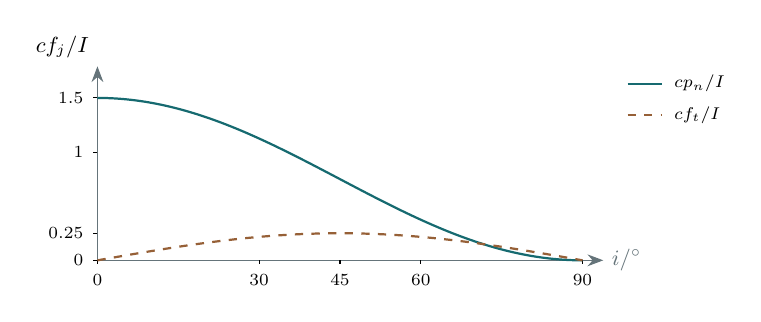
\begin{tikzpicture}[scale=.88,transform shape]
\draw[axis] (0,0.0)--(7.3,0.0) node[right] {$i/{}^\circ$};
\draw[axis] (0,0)--(0,2.8);
\node[above left] at (0,2.8) {$cf_j/I$};
\draw[thin] (0.000000,0.0)--(0.000000,-0.06);\node[below,font=\scriptsize] at (0.000000,-0.08) {$ 0 $};
\draw[thin] (2.333333,0.0)--(2.333333,-0.06);\node[below,font=\scriptsize] at (2.333333,-0.08) {$ 30 $};
\draw[thin] (3.500000,0.0)--(3.500000,-0.06);\node[below,font=\scriptsize] at (3.500000,-0.08) {$ 45 $};
\draw[thin] (4.666667,0.0)--(4.666667,-0.06);\node[below,font=\scriptsize] at (4.666667,-0.08) {$ 60 $};
\draw[thin] (7.000000,0.0)--(7.000000,-0.06);\node[below,font=\scriptsize] at (7.000000,-0.08) {$ 90 $};
\draw[thin] (0,0.000000)--(-.06,0.000000);\node[left,font=\scriptsize] at (-.08,0.000000) {$ 0 $};
\draw[thin] (0,0.390625)--(-.06,0.390625);\node[left,font=\scriptsize] at (-.08,0.390625) {$ 0.25 $};
\draw[thin] (0,1.562500)--(-.06,1.562500);\node[left,font=\scriptsize] at (-.08,1.562500) {$ 1 $};
\draw[thin] (0,2.343750)--(-.06,2.343750);\node[left,font=\scriptsize] at (-.08,2.343750) {$ 1.5 $};
\draw[thick,color=accent] plot coordinates {(0.0000000,2.3437500) (0.0291667,2.3436496) (0.0583333,2.3433484) (0.0875000,2.3428465) (0.1166667,2.3421440) (0.1458333,2.3412409) (0.1750000,2.3401375) (0.2041667,2.3388339) (0.2333333,2.3373303) (0.2625000,2.3356271) (0.2916667,2.3337244) (0.3208333,2.3316227) (0.3500000,2.3293223) (0.3791667,2.3268235) (0.4083333,2.3241268) (0.4375000,2.3212328) (0.4666667,2.3181417) (0.4958333,2.3148543) (0.5250000,2.3113710) (0.5541667,2.3076925) (0.5833333,2.3038193) (0.6125000,2.2997522) (0.6416667,2.2954919) (0.6708333,2.2910390) (0.7000000,2.2863944) (0.7291667,2.2815587) (0.7583333,2.2765330) (0.7875000,2.2713180) (0.8166667,2.2659146) (0.8458333,2.2603237) (0.8750000,2.2545463) (0.9041667,2.2485834) (0.9333333,2.2424361) (0.9625000,2.2361053) (0.9916667,2.2295921) (1.0208333,2.2228977) (1.0500000,2.2160233) (1.0791667,2.2089699) (1.1083333,2.2017388) (1.1375000,2.1943313) (1.1666667,2.1867485) (1.1958333,2.1789919) (1.2250000,2.1710627) (1.2541667,2.1629623) (1.2833333,2.1546921) (1.3125000,2.1462535) (1.3416667,2.1376479) (1.3708333,2.1288768) (1.4000000,2.1199418) (1.4291667,2.1108443) (1.4583333,2.1015859) (1.4875000,2.0921683) (1.5166667,2.0825929) (1.5458333,2.0728615) (1.5750000,2.0629757) (1.6041667,2.0529373) (1.6333333,2.0427478) (1.6625000,2.0324092) (1.6916667,2.0219231) (1.7208333,2.0112913) (1.7500000,2.0005158) (1.7791667,1.9895982) (1.8083333,1.9785405) (1.8375000,1.9673446) (1.8666667,1.9560124) (1.8958333,1.9445459) (1.9250000,1.9329469) (1.9541667,1.9212176) (1.9833333,1.9093598) (2.0125000,1.8973757) (2.0416667,1.8852673) (2.0708333,1.8730366) (2.1000000,1.8606858) (2.1291667,1.8482170) (2.1583333,1.8356323) (2.1875000,1.8229339) (2.2166667,1.8101239) (2.2458333,1.7972045) (2.2750000,1.7841780) (2.3041667,1.7710466) (2.3333333,1.7578125) (2.3625000,1.7444780) (2.3916667,1.7310454) (2.4208333,1.7175170) (2.4500000,1.7038951) (2.4791667,1.6901821) (2.5083333,1.6763802) (2.5375000,1.6624919) (2.5666667,1.6485195) (2.5958333,1.6344655) (2.6250000,1.6203321) (2.6541667,1.6061220) (2.6833333,1.5918374) (2.7125000,1.5774809) (2.7416667,1.5630549) (2.7708333,1.5485619) (2.8000000,1.5340043) (2.8291667,1.5193847) (2.8583333,1.5047055) (2.8875000,1.4899693) (2.9166667,1.4751786) (2.9458333,1.4603359) (2.9750000,1.4454438) (3.0041667,1.4305048) (3.0333333,1.4155215) (3.0625000,1.4004965) (3.0916667,1.3854323) (3.1208333,1.3703314) (3.1500000,1.3551966) (3.1791667,1.3400304) (3.2083333,1.3248354) (3.2375000,1.3096141) (3.2666667,1.2943693) (3.2958333,1.2791035) (3.3250000,1.2638193) (3.3541667,1.2485193) (3.3833333,1.2332062) (3.4125000,1.2178826) (3.4416667,1.2025511) (3.4708333,1.1872144) (3.5000000,1.1718750) (3.5291667,1.1565356) (3.5583333,1.1411989) (3.5875000,1.1258674) (3.6166667,1.1105438) (3.6458333,1.0952307) (3.6750000,1.0799307) (3.7041667,1.0646465) (3.7333333,1.0493807) (3.7625000,1.0341359) (3.7916667,1.0189146) (3.8208333,1.0037196) (3.8500000,0.9885534) (3.8791667,0.9734186) (3.9083333,0.9583177) (3.9375000,0.9432535) (3.9666667,0.9282285) (3.9958333,0.9132452) (4.0250000,0.8983062) (4.0541667,0.8834141) (4.0833333,0.8685714) (4.1125000,0.8537807) (4.1416667,0.8390445) (4.1708333,0.8243653) (4.2000000,0.8097457) (4.2291667,0.7951881) (4.2583333,0.7806951) (4.2875000,0.7662691) (4.3166667,0.7519126) (4.3458333,0.7376280) (4.3750000,0.7234179) (4.4041667,0.7092845) (4.4333333,0.6952305) (4.4625000,0.6812581) (4.4916667,0.6673698) (4.5208333,0.6535679) (4.5500000,0.6398549) (4.5791667,0.6262330) (4.6083333,0.6127046) (4.6375000,0.5992720) (4.6666667,0.5859375) (4.6958333,0.5727034) (4.7250000,0.5595720) (4.7541667,0.5465455) (4.7833333,0.5336261) (4.8125000,0.5208161) (4.8416667,0.5081177) (4.8708333,0.4955330) (4.9000000,0.4830642) (4.9291667,0.4707134) (4.9583333,0.4584827) (4.9875000,0.4463743) (5.0166667,0.4343902) (5.0458333,0.4225324) (5.0750000,0.4108031) (5.1041667,0.3992041) (5.1333333,0.3877376) (5.1625000,0.3764054) (5.1916667,0.3652095) (5.2208333,0.3541518) (5.2500000,0.3432342) (5.2791667,0.3324587) (5.3083333,0.3218269) (5.3375000,0.3113408) (5.3666667,0.3010022) (5.3958333,0.2908127) (5.4250000,0.2807743) (5.4541667,0.2708885) (5.4833333,0.2611571) (5.5125000,0.2515817) (5.5416667,0.2421641) (5.5708333,0.2329057) (5.6000000,0.2238082) (5.6291667,0.2148732) (5.6583333,0.2061021) (5.6875000,0.1974965) (5.7166667,0.1890579) (5.7458333,0.1807877) (5.7750000,0.1726873) (5.8041667,0.1647581) (5.8333333,0.1570015) (5.8625000,0.1494187) (5.8916667,0.1420112) (5.9208333,0.1347801) (5.9500000,0.1277267) (5.9791667,0.1208523) (6.0083333,0.1141579) (6.0375000,0.1076447) (6.0666667,0.1013139) (6.0958333,0.0951666) (6.1250000,0.0892037) (6.1541667,0.0834263) (6.1833333,0.0778354) (6.2125000,0.0724320) (6.2416667,0.0672170) (6.2708333,0.0621913) (6.3000000,0.0573556) (6.3291667,0.0527110) (6.3583333,0.0482581) (6.3875000,0.0439978) (6.4166667,0.0399307) (6.4458333,0.0360575) (6.4750000,0.0323790) (6.5041667,0.0288957) (6.5333333,0.0256083) (6.5625000,0.0225172) (6.5916667,0.0196232) (6.6208333,0.0169265) (6.6500000,0.0144277) (6.6791667,0.0121273) (6.7083333,0.0100256) (6.7375000,0.0081229) (6.7666667,0.0064197) (6.7958333,0.0049161) (6.8250000,0.0036125) (6.8541667,0.0025091) (6.8833333,0.0016060) (6.9125000,0.0009035) (6.9416667,0.0004016) (6.9708333,0.0001004) (7.0000000,0.0000000)};
\draw[thick,color=accent] (7.65,2.55)--(8.15,2.55);\node[right,font=\scriptsize] at (8.2,2.55) {$cp_n/I$};
\draw[thick,dashed,color=warm] plot coordinates {(0.0000000,0.0000000) (0.0291667,0.0051131) (0.0583333,0.0102254) (0.0875000,0.0153359) (0.1166667,0.0204437) (0.1458333,0.0255481) (0.1750000,0.0306481) (0.2041667,0.0357428) (0.2333333,0.0408314) (0.2625000,0.0459130) (0.2916667,0.0509868) (0.3208333,0.0560518) (0.3500000,0.0611072) (0.3791667,0.0661521) (0.4083333,0.0711858) (0.4375000,0.0762072) (0.4666667,0.0812155) (0.4958333,0.0862099) (0.5250000,0.0911896) (0.5541667,0.0961536) (0.5833333,0.1011012) (0.6125000,0.1060314) (0.6416667,0.1109435) (0.6708333,0.1158366) (0.7000000,0.1207098) (0.7291667,0.1255623) (0.7583333,0.1303933) (0.7875000,0.1352020) (0.8166667,0.1399875) (0.8458333,0.1447490) (0.8750000,0.1494857) (0.9041667,0.1541968) (0.9333333,0.1588815) (0.9625000,0.1635390) (0.9916667,0.1681684) (1.0208333,0.1727690) (1.0500000,0.1773400) (1.0791667,0.1818807) (1.1083333,0.1863901) (1.1375000,0.1908677) (1.1666667,0.1953125) (1.1958333,0.1997239) (1.2250000,0.2041010) (1.2541667,0.2084432) (1.2833333,0.2127496) (1.3125000,0.2170196) (1.3416667,0.2212524) (1.3708333,0.2254473) (1.4000000,0.2296036) (1.4291667,0.2337205) (1.4583333,0.2377974) (1.4875000,0.2418336) (1.5166667,0.2458283) (1.5458333,0.2497809) (1.5750000,0.2536906) (1.6041667,0.2575570) (1.6333333,0.2613791) (1.6625000,0.2651565) (1.6916667,0.2688885) (1.7208333,0.2725744) (1.7500000,0.2762136) (1.7791667,0.2798054) (1.8083333,0.2833494) (1.8375000,0.2868447) (1.8666667,0.2902909) (1.8958333,0.2936874) (1.9250000,0.2970336) (1.9541667,0.3003288) (1.9833333,0.3035726) (2.0125000,0.3067644) (2.0416667,0.3099036) (2.0708333,0.3129898) (2.1000000,0.3160223) (2.1291667,0.3190006) (2.1583333,0.3219243) (2.1875000,0.3247928) (2.2166667,0.3276057) (2.2458333,0.3303624) (2.2750000,0.3330626) (2.3041667,0.3357056) (2.3333333,0.3382912) (2.3625000,0.3408188) (2.3916667,0.3432879) (2.4208333,0.3456983) (2.4500000,0.3480494) (2.4791667,0.3503409) (2.5083333,0.3525724) (2.5375000,0.3547434) (2.5666667,0.3568537) (2.5958333,0.3589028) (2.6250000,0.3608904) (2.6541667,0.3628162) (2.6833333,0.3646799) (2.7125000,0.3664810) (2.7416667,0.3682193) (2.7708333,0.3698946) (2.8000000,0.3715065) (2.8291667,0.3730547) (2.8583333,0.3745390) (2.8875000,0.3759591) (2.9166667,0.3773148) (2.9458333,0.3786058) (2.9750000,0.3798320) (3.0041667,0.3809931) (3.0333333,0.3820889) (3.0625000,0.3831193) (3.0916667,0.3840839) (3.1208333,0.3849828) (3.1500000,0.3858158) (3.1791667,0.3865826) (3.2083333,0.3872831) (3.2375000,0.3879174) (3.2666667,0.3884851) (3.2958333,0.3889863) (3.3250000,0.3894208) (3.3541667,0.3897886) (3.3833333,0.3900897) (3.4125000,0.3903238) (3.4416667,0.3904911) (3.4708333,0.3905915) (3.5000000,0.3906250) (3.5291667,0.3905915) (3.5583333,0.3904911) (3.5875000,0.3903238) (3.6166667,0.3900897) (3.6458333,0.3897886) (3.6750000,0.3894208) (3.7041667,0.3889863) (3.7333333,0.3884851) (3.7625000,0.3879174) (3.7916667,0.3872831) (3.8208333,0.3865826) (3.8500000,0.3858158) (3.8791667,0.3849828) (3.9083333,0.3840839) (3.9375000,0.3831193) (3.9666667,0.3820889) (3.9958333,0.3809931) (4.0250000,0.3798320) (4.0541667,0.3786058) (4.0833333,0.3773148) (4.1125000,0.3759591) (4.1416667,0.3745390) (4.1708333,0.3730547) (4.2000000,0.3715065) (4.2291667,0.3698946) (4.2583333,0.3682193) (4.2875000,0.3664810) (4.3166667,0.3646799) (4.3458333,0.3628162) (4.3750000,0.3608904) (4.4041667,0.3589028) (4.4333333,0.3568537) (4.4625000,0.3547434) (4.4916667,0.3525724) (4.5208333,0.3503409) (4.5500000,0.3480494) (4.5791667,0.3456983) (4.6083333,0.3432879) (4.6375000,0.3408188) (4.6666667,0.3382912) (4.6958333,0.3357056) (4.7250000,0.3330626) (4.7541667,0.3303624) (4.7833333,0.3276057) (4.8125000,0.3247928) (4.8416667,0.3219243) (4.8708333,0.3190006) (4.9000000,0.3160223) (4.9291667,0.3129898) (4.9583333,0.3099036) (4.9875000,0.3067644) (5.0166667,0.3035726) (5.0458333,0.3003288) (5.0750000,0.2970336) (5.1041667,0.2936874) (5.1333333,0.2902909) (5.1625000,0.2868447) (5.1916667,0.2833494) (5.2208333,0.2798054) (5.2500000,0.2762136) (5.2791667,0.2725744) (5.3083333,0.2688885) (5.3375000,0.2651565) (5.3666667,0.2613791) (5.3958333,0.2575570) (5.4250000,0.2536906) (5.4541667,0.2497809) (5.4833333,0.2458283) (5.5125000,0.2418336) (5.5416667,0.2377974) (5.5708333,0.2337205) (5.6000000,0.2296036) (5.6291667,0.2254473) (5.6583333,0.2212524) (5.6875000,0.2170196) (5.7166667,0.2127496) (5.7458333,0.2084432) (5.7750000,0.2041010) (5.8041667,0.1997239) (5.8333333,0.1953125) (5.8625000,0.1908677) (5.8916667,0.1863901) (5.9208333,0.1818807) (5.9500000,0.1773400) (5.9791667,0.1727690) (6.0083333,0.1681684) (6.0375000,0.1635390) (6.0666667,0.1588815) (6.0958333,0.1541968) (6.1250000,0.1494857) (6.1541667,0.1447490) (6.1833333,0.1399875) (6.2125000,0.1352020) (6.2416667,0.1303933) (6.2708333,0.1255623) (6.3000000,0.1207098) (6.3291667,0.1158366) (6.3583333,0.1109435) (6.3875000,0.1060314) (6.4166667,0.1011012) (6.4458333,0.0961536) (6.4750000,0.0911896) (6.5041667,0.0862099) (6.5333333,0.0812155) (6.5625000,0.0762072) (6.5916667,0.0711858) (6.6208333,0.0661521) (6.6500000,0.0611072) (6.6791667,0.0560518) (6.7083333,0.0509868) (6.7375000,0.0459130) (6.7666667,0.0408314) (6.7958333,0.0357428) (6.8250000,0.0306481) (6.8541667,0.0255481) (6.8833333,0.0204437) (6.9125000,0.0153359) (6.9416667,0.0102254) (6.9708333,0.0051131) (7.0000000,0.0000000)};
\draw[thick,dashed,color=warm] (7.65,2.0999999999999996)--(8.15,2.0999999999999996);\node[right,font=\scriptsize] at (8.2,2.0999999999999996) {$cf_t/I$};
\end{tikzpicture}
\figcaption{变图近1.1V3\quad 固定光束强度I下切向力峰值与法向单调变化}
\end{minipage}\end{center}
\item \textbf{Lambert漫反射。}表面按外法线轴对称Lambert分布反射，反射总功率为$RJ\dd S$，入射功率密度为$J$。求平均反射动量及两力分量。

归一化角概率为$\cos\vartheta\,\dd\Omega/\pi$，故平均外法向方向余弦为
\[
 \langle\cos\vartheta\rangle=\frac{2\pi}{\pi}
 \int_0^{\pi/2}\cos^2\vartheta\sin\vartheta\dd\vartheta=\frac23.
\]
方位对称使出射平均切向动量为零，因而$p_n=J(\cos i+2R/3)/c$、$f_t=J\sin i/c$。变图近1.1V4比较$R=1/2$的漫反射与镜面法向压力；差别由实际出射角分布给出。
\begin{center}\begin{minipage}{.98\linewidth}\centering
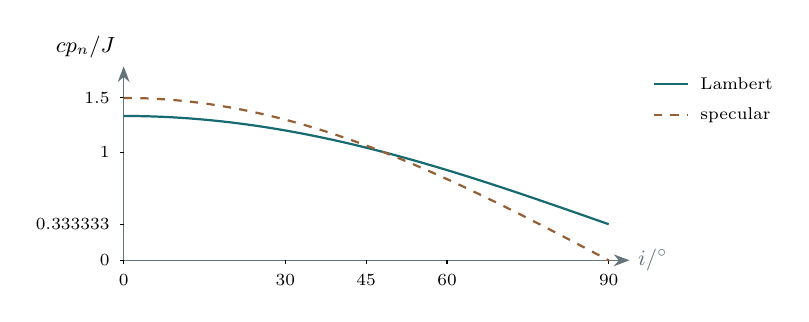
\begin{tikzpicture}[scale=.88,transform shape]
\draw[axis] (0,0.0)--(7.3,0.0) node[right] {$i/{}^\circ$};
\draw[axis] (0,0)--(0,2.8);
\node[above left] at (0,2.8) {$cp_n/J$};
\draw[thin] (0.000000,0.0)--(0.000000,-0.06);\node[below,font=\scriptsize] at (0.000000,-0.08) {$ 0 $};
\draw[thin] (2.333333,0.0)--(2.333333,-0.06);\node[below,font=\scriptsize] at (2.333333,-0.08) {$ 30 $};
\draw[thin] (3.500000,0.0)--(3.500000,-0.06);\node[below,font=\scriptsize] at (3.500000,-0.08) {$ 45 $};
\draw[thin] (4.666667,0.0)--(4.666667,-0.06);\node[below,font=\scriptsize] at (4.666667,-0.08) {$ 60 $};
\draw[thin] (7.000000,0.0)--(7.000000,-0.06);\node[below,font=\scriptsize] at (7.000000,-0.08) {$ 90 $};
\draw[thin] (0,0.000000)--(-.06,0.000000);\node[left,font=\scriptsize] at (-.08,0.000000) {$ 0 $};
\draw[thin] (0,0.520833)--(-.06,0.520833);\node[left,font=\scriptsize] at (-.08,0.520833) {$ 0.333333 $};
\draw[thin] (0,1.562500)--(-.06,1.562500);\node[left,font=\scriptsize] at (-.08,1.562500) {$ 1 $};
\draw[thin] (0,2.343750)--(-.06,2.343750);\node[left,font=\scriptsize] at (-.08,2.343750) {$ 1.5 $};
\draw[thick,color=accent] plot coordinates {(0.0000000,2.0833333) (0.0291667,2.0832999) (0.0583333,2.0831995) (0.0875000,2.0830321) (0.1166667,2.0827979) (0.1458333,2.0824968) (0.1750000,2.0821287) (0.2041667,2.0816938) (0.2333333,2.0811920) (0.2625000,2.0806233) (0.2916667,2.0799879) (0.3208333,2.0792857) (0.3500000,2.0785167) (0.3791667,2.0776809) (0.4083333,2.0767785) (0.4375000,2.0758095) (0.4666667,2.0747738) (0.4958333,2.0736716) (0.5250000,2.0725028) (0.5541667,2.0712676) (0.5833333,2.0699659) (0.6125000,2.0685979) (0.6416667,2.0671636) (0.6708333,2.0656631) (0.7000000,2.0640964) (0.7291667,2.0624635) (0.7583333,2.0607647) (0.7875000,2.0589998) (0.8166667,2.0571691) (0.8458333,2.0552726) (0.8750000,2.0533103) (0.9041667,2.0512824) (0.9333333,2.0491890) (0.9625000,2.0470300) (0.9916667,2.0448057) (1.0208333,2.0425161) (1.0500000,2.0401613) (1.0791667,2.0377415) (1.1083333,2.0352566) (1.1375000,2.0327069) (1.1666667,2.0300924) (1.1958333,2.0274133) (1.2250000,2.0246696) (1.2541667,2.0218616) (1.2833333,2.0189892) (1.3125000,2.0160526) (1.3416667,2.0130520) (1.3708333,2.0099875) (1.4000000,2.0068591) (1.4291667,2.0036672) (1.4583333,2.0004117) (1.4875000,1.9970928) (1.5166667,1.9937107) (1.5458333,1.9902655) (1.5750000,1.9867573) (1.6041667,1.9831863) (1.6333333,1.9795527) (1.6625000,1.9758567) (1.6916667,1.9720983) (1.7208333,1.9682777) (1.7500000,1.9643951) (1.7791667,1.9604507) (1.8083333,1.9564446) (1.8375000,1.9523770) (1.8666667,1.9482481) (1.8958333,1.9440581) (1.9250000,1.9398070) (1.9541667,1.9354952) (1.9833333,1.9311228) (2.0125000,1.9266900) (2.0416667,1.9221970) (2.0708333,1.9176439) (2.1000000,1.9130310) (2.1291667,1.9083585) (2.1583333,1.9036265) (2.1875000,1.8988353) (2.2166667,1.8939851) (2.2458333,1.8890760) (2.2750000,1.8841083) (2.3041667,1.8790823) (2.3333333,1.8739980) (2.3625000,1.8688558) (2.3916667,1.8636559) (2.4208333,1.8583984) (2.4500000,1.8530836) (2.4791667,1.8477117) (2.5083333,1.8422831) (2.5375000,1.8367978) (2.5666667,1.8312561) (2.5958333,1.8256583) (2.6250000,1.8200046) (2.6541667,1.8142953) (2.6833333,1.8085305) (2.7125000,1.8027106) (2.7416667,1.7968358) (2.7708333,1.7909063) (2.8000000,1.7849224) (2.8291667,1.7788843) (2.8583333,1.7727924) (2.8875000,1.7666469) (2.9166667,1.7604479) (2.9458333,1.7541959) (2.9750000,1.7478910) (3.0041667,1.7415336) (3.0333333,1.7351239) (3.0625000,1.7286622) (3.0916667,1.7221487) (3.1208333,1.7155838) (3.1500000,1.7089677) (3.1791667,1.7023006) (3.2083333,1.6955830) (3.2375000,1.6888151) (3.2666667,1.6819971) (3.2958333,1.6751294) (3.3250000,1.6682123) (3.3541667,1.6612459) (3.3833333,1.6542308) (3.4125000,1.6471671) (3.4416667,1.6400551) (3.4708333,1.6328952) (3.5000000,1.6256877) (3.5291667,1.6184328) (3.5583333,1.6111309) (3.5875000,1.6037823) (3.6166667,1.5963874) (3.6458333,1.5889463) (3.6750000,1.5814595) (3.7041667,1.5739273) (3.7333333,1.5663499) (3.7625000,1.5587278) (3.7916667,1.5510612) (3.8208333,1.5433504) (3.8500000,1.5355959) (3.8791667,1.5277979) (3.9083333,1.5199568) (3.9375000,1.5120728) (3.9666667,1.5041464) (3.9958333,1.4961779) (4.0250000,1.4881676) (4.0541667,1.4801159) (4.0833333,1.4720231) (4.1125000,1.4638895) (4.1416667,1.4557155) (4.1708333,1.4475015) (4.2000000,1.4392478) (4.2291667,1.4309547) (4.2583333,1.4226227) (4.2875000,1.4142520) (4.3166667,1.4058431) (4.3458333,1.3973962) (4.3750000,1.3889118) (4.4041667,1.3803902) (4.4333333,1.3718318) (4.4625000,1.3632370) (4.4916667,1.3546060) (4.5208333,1.3459393) (4.5500000,1.3372373) (4.5791667,1.3285004) (4.6083333,1.3197288) (4.6375000,1.3109230) (4.6666667,1.3020833) (4.6958333,1.2932102) (4.7250000,1.2843040) (4.7541667,1.2753651) (4.7833333,1.2663939) (4.8125000,1.2573907) (4.8416667,1.2483560) (4.8708333,1.2392901) (4.9000000,1.2301935) (4.9291667,1.2210664) (4.9583333,1.2119094) (4.9875000,1.2027228) (5.0166667,1.1935069) (5.0458333,1.1842623) (5.0750000,1.1749892) (5.1041667,1.1656881) (5.1333333,1.1563593) (5.1625000,1.1470034) (5.1916667,1.1376206) (5.2208333,1.1282114) (5.2500000,1.1187762) (5.2791667,1.1093154) (5.3083333,1.0998293) (5.3375000,1.0903185) (5.3666667,1.0807833) (5.3958333,1.0712240) (5.4250000,1.0616412) (5.4541667,1.0520353) (5.4833333,1.0424066) (5.5125000,1.0327555) (5.5416667,1.0230825) (5.5708333,1.0133880) (5.6000000,1.0036724) (5.6291667,0.9939361) (5.6583333,0.9841795) (5.6875000,0.9744031) (5.7166667,0.9646073) (5.7458333,0.9547925) (5.7750000,0.9449590) (5.8041667,0.9351074) (5.8333333,0.9252381) (5.8625000,0.9153514) (5.8916667,0.9054479) (5.9208333,0.8955278) (5.9500000,0.8855917) (5.9791667,0.8756400) (6.0083333,0.8656731) (6.0375000,0.8556914) (6.0666667,0.8456954) (6.0958333,0.8356854) (6.1250000,0.8256620) (6.1541667,0.8156255) (6.1833333,0.8055763) (6.2125000,0.7955150) (6.2416667,0.7854419) (6.2708333,0.7753575) (6.3000000,0.7652622) (6.3291667,0.7551564) (6.3583333,0.7450406) (6.3875000,0.7349151) (6.4166667,0.7247805) (6.4458333,0.7146372) (6.4750000,0.7044855) (6.5041667,0.6943260) (6.5333333,0.6841591) (6.5625000,0.6739851) (6.5916667,0.6638046) (6.6208333,0.6536180) (6.6500000,0.6434257) (6.6791667,0.6332281) (6.7083333,0.6230257) (6.7375000,0.6128190) (6.7666667,0.6026083) (6.7958333,0.5923941) (6.8250000,0.5821768) (6.8541667,0.5719569) (6.8833333,0.5617348) (6.9125000,0.5515110) (6.9416667,0.5412858) (6.9708333,0.5310598) (7.0000000,0.5208333)};
\draw[thick,color=accent] (7.65,2.55)--(8.15,2.55);\node[right,font=\scriptsize] at (8.2,2.55) {$\mathrm{Lambert}$};
\draw[thick,dashed,color=warm] plot coordinates {(0.0000000,2.3437500) (0.0291667,2.3436998) (0.0583333,2.3435492) (0.0875000,2.3432982) (0.1166667,2.3429469) (0.1458333,2.3424951) (0.1750000,2.3419431) (0.2041667,2.3412907) (0.2333333,2.3405380) (0.2625000,2.3396850) (0.2916667,2.3387319) (0.3208333,2.3376785) (0.3500000,2.3365250) (0.3791667,2.3352714) (0.4083333,2.3339178) (0.4375000,2.3324642) (0.4666667,2.3309107) (0.4958333,2.3292573) (0.5250000,2.3275042) (0.5541667,2.3256514) (0.5833333,2.3236989) (0.6125000,2.3216469) (0.6416667,2.3194954) (0.6708333,2.3172446) (0.7000000,2.3148945) (0.7291667,2.3124453) (0.7583333,2.3098970) (0.7875000,2.3072498) (0.8166667,2.3045037) (0.8458333,2.3016589) (0.8750000,2.2987155) (0.9041667,2.2956736) (0.9333333,2.2925334) (0.9625000,2.2892950) (0.9916667,2.2859586) (1.0208333,2.2825242) (1.0500000,2.2789920) (1.0791667,2.2753622) (1.1083333,2.2716349) (1.1375000,2.2678104) (1.1666667,2.2638887) (1.1958333,2.2598700) (1.2250000,2.2557545) (1.2541667,2.2515423) (1.2833333,2.2472338) (1.3125000,2.2428289) (1.3416667,2.2383280) (1.3708333,2.2337312) (1.4000000,2.2290387) (1.4291667,2.2242507) (1.4583333,2.2193675) (1.4875000,2.2143892) (1.5166667,2.2093160) (1.5458333,2.2041482) (1.5750000,2.1988859) (1.6041667,2.1935295) (1.6333333,2.1880791) (1.6625000,2.1825350) (1.6916667,2.1768974) (1.7208333,2.1711665) (1.7500000,2.1653427) (1.7791667,2.1594260) (1.8083333,2.1534169) (1.8375000,2.1473155) (1.8666667,2.1411222) (1.8958333,2.1348371) (1.9250000,2.1284606) (1.9541667,2.1219929) (1.9833333,2.1154343) (2.0125000,2.1087850) (2.0416667,2.1020455) (2.0708333,2.0952159) (2.1000000,2.0882965) (2.1291667,2.0812877) (2.1583333,2.0741898) (2.1875000,2.0670030) (2.2166667,2.0597276) (2.2458333,2.0523640) (2.2750000,2.0449125) (2.3041667,2.0373734) (2.3333333,2.0297470) (2.3625000,2.0220337) (2.3916667,2.0142338) (2.4208333,2.0063476) (2.4500000,1.9983754) (2.4791667,1.9903176) (2.5083333,1.9821746) (2.5375000,1.9739466) (2.5666667,1.9656341) (2.5958333,1.9572374) (2.6250000,1.9487569) (2.6541667,1.9401929) (2.6833333,1.9315458) (2.7125000,1.9228159) (2.7416667,1.9140036) (2.7708333,1.9051094) (2.8000000,1.8961336) (2.8291667,1.8870765) (2.8583333,1.8779386) (2.8875000,1.8687203) (2.9166667,1.8594219) (2.9458333,1.8500438) (2.9750000,1.8405866) (3.0041667,1.8310504) (3.0333333,1.8214358) (3.0625000,1.8117433) (3.0916667,1.8019730) (3.1208333,1.7921256) (3.1500000,1.7822015) (3.1791667,1.7722010) (3.2083333,1.7621245) (3.2375000,1.7519726) (3.2666667,1.7417457) (3.2958333,1.7314441) (3.3250000,1.7210684) (3.3541667,1.7106189) (3.3833333,1.7000962) (3.4125000,1.6895006) (3.4416667,1.6788327) (3.4708333,1.6680928) (3.5000000,1.6572815) (3.5291667,1.6463992) (3.5583333,1.6354464) (3.5875000,1.6244235) (3.6166667,1.6133310) (3.6458333,1.6021695) (3.6750000,1.5909392) (3.7041667,1.5796409) (3.7333333,1.5682749) (3.7625000,1.5568417) (3.7916667,1.5453418) (3.8208333,1.5337757) (3.8500000,1.5221439) (3.8791667,1.5104469) (3.9083333,1.4986852) (3.9375000,1.4868593) (3.9666667,1.4749697) (3.9958333,1.4630169) (4.0250000,1.4510014) (4.0541667,1.4389238) (4.0833333,1.4267846) (4.1125000,1.4145842) (4.1416667,1.4023233) (4.1708333,1.3900023) (4.2000000,1.3776217) (4.2291667,1.3651821) (4.2583333,1.3526840) (4.2875000,1.3401280) (4.3166667,1.3275146) (4.3458333,1.3148443) (4.3750000,1.3021177) (4.4041667,1.2893354) (4.4333333,1.2764977) (4.4625000,1.2636054) (4.4916667,1.2506590) (4.5208333,1.2376590) (4.5500000,1.2246060) (4.5791667,1.2115005) (4.6083333,1.1983432) (4.6375000,1.1851345) (4.6666667,1.1718750) (4.6958333,1.1585653) (4.7250000,1.1452060) (4.7541667,1.1317977) (4.7833333,1.1183408) (4.8125000,1.1048361) (4.8416667,1.0912840) (4.8708333,1.0776852) (4.9000000,1.0640402) (4.9291667,1.0503497) (4.9583333,1.0366141) (4.9875000,1.0228342) (5.0166667,1.0090104) (5.0458333,0.9951434) (5.0750000,0.9812338) (5.1041667,0.9672821) (5.1333333,0.9532890) (5.1625000,0.9392551) (5.1916667,0.9251809) (5.2208333,0.9110671) (5.2500000,0.8969143) (5.2791667,0.8827231) (5.3083333,0.8684940) (5.3375000,0.8542277) (5.3666667,0.8399249) (5.3958333,0.8255860) (5.4250000,0.8112119) (5.4541667,0.7968029) (5.4833333,0.7823598) (5.5125000,0.7678832) (5.5416667,0.7533737) (5.5708333,0.7388320) (5.6000000,0.7242586) (5.6291667,0.7096541) (5.6583333,0.6950193) (5.6875000,0.6803547) (5.7166667,0.6656610) (5.7458333,0.6509387) (5.7750000,0.6361886) (5.8041667,0.6214112) (5.8333333,0.6066071) (5.8625000,0.5917771) (5.8916667,0.5769218) (5.9208333,0.5620417) (5.9500000,0.5471376) (5.9791667,0.5322100) (6.0083333,0.5172596) (6.0375000,0.5022871) (6.0666667,0.4872930) (6.0958333,0.4722781) (6.1250000,0.4572429) (6.1541667,0.4421882) (6.1833333,0.4271145) (6.2125000,0.4120225) (6.2416667,0.3969129) (6.2708333,0.3817863) (6.3000000,0.3666433) (6.3291667,0.3514846) (6.3583333,0.3363108) (6.3875000,0.3211227) (6.4166667,0.3059208) (6.4458333,0.2907057) (6.4750000,0.2754783) (6.5041667,0.2602390) (6.5333333,0.2449886) (6.5625000,0.2297277) (6.5916667,0.2144569) (6.6208333,0.1991770) (6.6500000,0.1838885) (6.6791667,0.1685922) (6.7083333,0.1532886) (6.7375000,0.1379784) (6.7666667,0.1226624) (6.7958333,0.1073411) (6.8250000,0.0920152) (6.8541667,0.0766854) (6.8833333,0.0613522) (6.9125000,0.0460165) (6.9416667,0.0306787) (6.9708333,0.0153397) (7.0000000,0.0000000)};
\draw[thick,dashed,color=warm] (7.65,2.0999999999999996)--(8.15,2.0999999999999996);\node[right,font=\scriptsize] at (8.2,2.0999999999999996) {$\mathrm{specular}$};
\end{tikzpicture}
\figcaption{变图近1.1V4\quad 固定J且反射率一半时出射角分布改变平均反冲}
\end{minipage}\end{center}
\item \textbf{还可透射的平行薄片。}入射、反射、最终透射均在真空中，反射率$R$、透射率$T$、吸收率$A=1-R-T$，最终透射方向与入射方向相同。求薄片两力密度。

每单位时间由入射扣去反射和透射的动量通量，得到
\[
 \boldsymbol f=\frac{I\cos i}{c}
 [\hat{\boldsymbol k}_i-R\hat{\boldsymbol k}_r-T\hat{\boldsymbol k}_i],
 \quad p_n=\frac Ic(A+2R)\cos^2i,\quad
 f_t=\frac IcA\sin i\cos i.
\]
变图近1.1V5取$R=0.2,T=0.5,A=0.3$画两分量。反射仅改法向分量，同向透射保留透射光的两份动量，吸收部分留下切向力。
\begin{center}\begin{minipage}{.98\linewidth}\centering
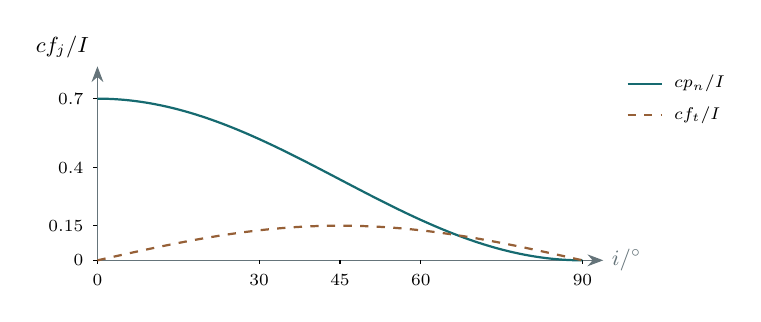
\begin{tikzpicture}[scale=.88,transform shape]
\draw[axis] (0,0.0)--(7.3,0.0) node[right] {$i/{}^\circ$};
\draw[axis] (0,0)--(0,2.8);
\node[above left] at (0,2.8) {$cf_j/I$};
\draw[thin] (0.000000,0.0)--(0.000000,-0.06);\node[below,font=\scriptsize] at (0.000000,-0.08) {$ 0 $};
\draw[thin] (2.333333,0.0)--(2.333333,-0.06);\node[below,font=\scriptsize] at (2.333333,-0.08) {$ 30 $};
\draw[thin] (3.500000,0.0)--(3.500000,-0.06);\node[below,font=\scriptsize] at (3.500000,-0.08) {$ 45 $};
\draw[thin] (4.666667,0.0)--(4.666667,-0.06);\node[below,font=\scriptsize] at (4.666667,-0.08) {$ 60 $};
\draw[thin] (7.000000,0.0)--(7.000000,-0.06);\node[below,font=\scriptsize] at (7.000000,-0.08) {$ 90 $};
\draw[thin] (0,0.000000)--(-.06,0.000000);\node[left,font=\scriptsize] at (-.08,0.000000) {$ 0 $};
\draw[thin] (0,0.500000)--(-.06,0.500000);\node[left,font=\scriptsize] at (-.08,0.500000) {$ 0.15 $};
\draw[thin] (0,1.333333)--(-.06,1.333333);\node[left,font=\scriptsize] at (-.08,1.333333) {$ 0.4 $};
\draw[thin] (0,2.333333)--(-.06,2.333333);\node[left,font=\scriptsize] at (-.08,2.333333) {$ 0.7 $};
\draw[thick,color=accent] plot coordinates {(0.0000000,2.3333333) (0.0291667,2.3332334) (0.0583333,2.3329335) (0.0875000,2.3324339) (0.1166667,2.3317345) (0.1458333,2.3308354) (0.1750000,2.3297369) (0.2041667,2.3284391) (0.2333333,2.3269422) (0.2625000,2.3252465) (0.2916667,2.3233523) (0.3208333,2.3212600) (0.3500000,2.3189697) (0.3791667,2.3164821) (0.4083333,2.3137974) (0.4375000,2.3109162) (0.4666667,2.3078389) (0.4958333,2.3045660) (0.5250000,2.3010982) (0.5541667,2.2974361) (0.5833333,2.2935801) (0.6125000,2.2895311) (0.6416667,2.2852897) (0.6708333,2.2808566) (0.7000000,2.2762326) (0.7291667,2.2714185) (0.7583333,2.2664151) (0.7875000,2.2612232) (0.8166667,2.2558438) (0.8458333,2.2502778) (0.8750000,2.2445261) (0.9041667,2.2385897) (0.9333333,2.2324697) (0.9625000,2.2261670) (0.9916667,2.2196828) (1.0208333,2.2130182) (1.0500000,2.2061743) (1.0791667,2.1991522) (1.1083333,2.1919533) (1.1375000,2.1845787) (1.1666667,2.1770296) (1.1958333,2.1693075) (1.2250000,2.1614135) (1.2541667,2.1533491) (1.2833333,2.1451157) (1.3125000,2.1367145) (1.3416667,2.1281472) (1.3708333,2.1194151) (1.4000000,2.1105198) (1.4291667,2.1014628) (1.4583333,2.0922456) (1.4875000,2.0828698) (1.5166667,2.0733370) (1.5458333,2.0636488) (1.5750000,2.0538070) (1.6041667,2.0438131) (1.6333333,2.0336690) (1.6625000,2.0233763) (1.6916667,2.0129368) (1.7208333,2.0023523) (1.7500000,1.9916246) (1.7791667,1.9807555) (1.8083333,1.9697470) (1.8375000,1.9586009) (1.8666667,1.9473190) (1.8958333,1.9359035) (1.9250000,1.9243561) (1.9541667,1.9126788) (1.9833333,1.9008738) (2.0125000,1.8889429) (2.0416667,1.8768883) (2.0708333,1.8647120) (2.1000000,1.8524161) (2.1291667,1.8400027) (2.1583333,1.8274739) (2.1875000,1.8148319) (2.2166667,1.8020789) (2.2458333,1.7892169) (2.2750000,1.7762483) (2.3041667,1.7631753) (2.3333333,1.7500000) (2.3625000,1.7367248) (2.3916667,1.7233519) (2.4208333,1.7098836) (2.4500000,1.6963222) (2.4791667,1.6826701) (2.5083333,1.6689296) (2.5375000,1.6551030) (2.5666667,1.6411928) (2.5958333,1.6272012) (2.6250000,1.6131307) (2.6541667,1.5989837) (2.6833333,1.5847626) (2.7125000,1.5704699) (2.7416667,1.5561080) (2.7708333,1.5416794) (2.8000000,1.5271865) (2.8291667,1.5126318) (2.8583333,1.4980179) (2.8875000,1.4833472) (2.9166667,1.4686222) (2.9458333,1.4538455) (2.9750000,1.4390196) (3.0041667,1.4241470) (3.0333333,1.4092303) (3.0625000,1.3942720) (3.0916667,1.3792748) (3.1208333,1.3642411) (3.1500000,1.3491735) (3.1791667,1.3340747) (3.2083333,1.3189472) (3.2375000,1.3037936) (3.2666667,1.2886165) (3.2958333,1.2734186) (3.3250000,1.2582023) (3.3541667,1.2429703) (3.3833333,1.2277253) (3.4125000,1.2124698) (3.4416667,1.1972064) (3.4708333,1.1819379) (3.5000000,1.1666667) (3.5291667,1.1513955) (3.5583333,1.1361269) (3.5875000,1.1208635) (3.6166667,1.1056081) (3.6458333,1.0903630) (3.6750000,1.0751311) (3.7041667,1.0599148) (3.7333333,1.0447168) (3.7625000,1.0295397) (3.7916667,1.0143861) (3.8208333,0.9992586) (3.8500000,0.9841598) (3.8791667,0.9690922) (3.9083333,0.9540586) (3.9375000,0.9390613) (3.9666667,0.9241030) (3.9958333,0.9091863) (4.0250000,0.8943137) (4.0541667,0.8794878) (4.0833333,0.8647111) (4.1125000,0.8499861) (4.1416667,0.8353154) (4.1708333,0.8207015) (4.2000000,0.8061468) (4.2291667,0.7916540) (4.2583333,0.7772253) (4.2875000,0.7628634) (4.3166667,0.7485707) (4.3458333,0.7343497) (4.3750000,0.7202027) (4.4041667,0.7061322) (4.4333333,0.6921406) (4.4625000,0.6782303) (4.4916667,0.6644037) (4.5208333,0.6506632) (4.5500000,0.6370111) (4.5791667,0.6234497) (4.6083333,0.6099814) (4.6375000,0.5966086) (4.6666667,0.5833333) (4.6958333,0.5701581) (4.7250000,0.5570850) (4.7541667,0.5441164) (4.7833333,0.5312545) (4.8125000,0.5185014) (4.8416667,0.5058594) (4.8708333,0.4933306) (4.9000000,0.4809172) (4.9291667,0.4686213) (4.9583333,0.4564450) (4.9875000,0.4443904) (5.0166667,0.4324595) (5.0458333,0.4206545) (5.0750000,0.4089773) (5.1041667,0.3974299) (5.1333333,0.3860143) (5.1625000,0.3747325) (5.1916667,0.3635863) (5.2208333,0.3525778) (5.2500000,0.3417088) (5.2791667,0.3309811) (5.3083333,0.3203966) (5.3375000,0.3099571) (5.3666667,0.2996644) (5.3958333,0.2895202) (5.4250000,0.2795264) (5.4541667,0.2696845) (5.4833333,0.2599964) (5.5125000,0.2504636) (5.5416667,0.2410878) (5.5708333,0.2318706) (5.6000000,0.2228135) (5.6291667,0.2139182) (5.6583333,0.2051861) (5.6875000,0.1966188) (5.7166667,0.1882177) (5.7458333,0.1799842) (5.7750000,0.1719198) (5.8041667,0.1640259) (5.8333333,0.1563037) (5.8625000,0.1487547) (5.8916667,0.1413800) (5.9208333,0.1341811) (5.9500000,0.1271591) (5.9791667,0.1203151) (6.0083333,0.1136505) (6.0375000,0.1071663) (6.0666667,0.1008636) (6.0958333,0.0947436) (6.1250000,0.0888072) (6.1541667,0.0830555) (6.1833333,0.0774895) (6.2125000,0.0721101) (6.2416667,0.0669183) (6.2708333,0.0619148) (6.3000000,0.0571007) (6.3291667,0.0524767) (6.3583333,0.0480436) (6.3875000,0.0438022) (6.4166667,0.0397532) (6.4458333,0.0358973) (6.4750000,0.0322351) (6.5041667,0.0287673) (6.5333333,0.0254945) (6.5625000,0.0224172) (6.5916667,0.0195359) (6.6208333,0.0168513) (6.6500000,0.0143636) (6.6791667,0.0120734) (6.7083333,0.0099810) (6.7375000,0.0080868) (6.7666667,0.0063911) (6.7958333,0.0048943) (6.8250000,0.0035964) (6.8541667,0.0024979) (6.8833333,0.0015989) (6.9125000,0.0008995) (6.9416667,0.0003998) (6.9708333,0.0001000) (7.0000000,0.0000000)};
\draw[thick,color=accent] (7.65,2.55)--(8.15,2.55);\node[right,font=\scriptsize] at (8.2,2.55) {$cp_n/I$};
\draw[thick,dashed,color=warm] plot coordinates {(0.0000000,0.0000000) (0.0291667,0.0065448) (0.0583333,0.0130885) (0.0875000,0.0196299) (0.1166667,0.0261680) (0.1458333,0.0327016) (0.1750000,0.0392295) (0.2041667,0.0457508) (0.2333333,0.0522642) (0.2625000,0.0587687) (0.2916667,0.0652631) (0.3208333,0.0717463) (0.3500000,0.0782172) (0.3791667,0.0846748) (0.4083333,0.0911178) (0.4375000,0.0975452) (0.4666667,0.1039558) (0.4958333,0.1103487) (0.5250000,0.1167227) (0.5541667,0.1230766) (0.5833333,0.1294095) (0.6125000,0.1357202) (0.6416667,0.1420077) (0.6708333,0.1482708) (0.7000000,0.1545085) (0.7291667,0.1607197) (0.7583333,0.1669034) (0.7875000,0.1730585) (0.8166667,0.1791840) (0.8458333,0.1852787) (0.8750000,0.1913417) (0.9041667,0.1973719) (0.9333333,0.2033683) (0.9625000,0.2093299) (0.9916667,0.2152555) (1.0208333,0.2211443) (1.0500000,0.2269952) (1.0791667,0.2328073) (1.1083333,0.2385794) (1.1375000,0.2443106) (1.1666667,0.2500000) (1.1958333,0.2556465) (1.2250000,0.2612493) (1.2541667,0.2668073) (1.2833333,0.2723195) (1.3125000,0.2777851) (1.3416667,0.2832031) (1.3708333,0.2885726) (1.4000000,0.2938926) (1.4291667,0.2991623) (1.4583333,0.3043807) (1.4875000,0.3095470) (1.5166667,0.3146602) (1.5458333,0.3197195) (1.5750000,0.3247240) (1.6041667,0.3296729) (1.6333333,0.3345653) (1.6625000,0.3394004) (1.6916667,0.3441773) (1.7208333,0.3488952) (1.7500000,0.3535534) (1.7791667,0.3581510) (1.8083333,0.3626872) (1.8375000,0.3671613) (1.8666667,0.3715724) (1.8958333,0.3759199) (1.9250000,0.3802030) (1.9541667,0.3844209) (1.9833333,0.3885730) (2.0125000,0.3926585) (2.0416667,0.3966767) (2.0708333,0.4006269) (2.1000000,0.4045085) (2.1291667,0.4083208) (2.1583333,0.4120631) (2.1875000,0.4157348) (2.2166667,0.4193353) (2.2458333,0.4228639) (2.2750000,0.4263201) (2.3041667,0.4297032) (2.3333333,0.4330127) (2.3625000,0.4362480) (2.3916667,0.4394086) (2.4208333,0.4424938) (2.4500000,0.4455033) (2.4791667,0.4484364) (2.5083333,0.4512926) (2.5375000,0.4540716) (2.5666667,0.4567727) (2.5958333,0.4593956) (2.6250000,0.4619398) (2.6541667,0.4644048) (2.6833333,0.4667902) (2.7125000,0.4690957) (2.7416667,0.4713207) (2.7708333,0.4734651) (2.8000000,0.4755283) (2.8291667,0.4775100) (2.8583333,0.4794099) (2.8875000,0.4812276) (2.9166667,0.4829629) (2.9458333,0.4846155) (2.9750000,0.4861850) (3.0041667,0.4876712) (3.0333333,0.4890738) (3.0625000,0.4903926) (3.0916667,0.4916275) (3.1208333,0.4927780) (3.1500000,0.4938442) (3.1791667,0.4948257) (3.2083333,0.4957224) (3.2375000,0.4965342) (3.2666667,0.4972609) (3.2958333,0.4979025) (3.3250000,0.4984587) (3.3541667,0.4989295) (3.3833333,0.4993148) (3.4125000,0.4996145) (3.4416667,0.4998287) (3.4708333,0.4999572) (3.5000000,0.5000000) (3.5291667,0.4999572) (3.5583333,0.4998287) (3.5875000,0.4996145) (3.6166667,0.4993148) (3.6458333,0.4989295) (3.6750000,0.4984587) (3.7041667,0.4979025) (3.7333333,0.4972609) (3.7625000,0.4965342) (3.7916667,0.4957224) (3.8208333,0.4948257) (3.8500000,0.4938442) (3.8791667,0.4927780) (3.9083333,0.4916275) (3.9375000,0.4903926) (3.9666667,0.4890738) (3.9958333,0.4876712) (4.0250000,0.4861850) (4.0541667,0.4846155) (4.0833333,0.4829629) (4.1125000,0.4812276) (4.1416667,0.4794099) (4.1708333,0.4775100) (4.2000000,0.4755283) (4.2291667,0.4734651) (4.2583333,0.4713207) (4.2875000,0.4690957) (4.3166667,0.4667902) (4.3458333,0.4644048) (4.3750000,0.4619398) (4.4041667,0.4593956) (4.4333333,0.4567727) (4.4625000,0.4540716) (4.4916667,0.4512926) (4.5208333,0.4484364) (4.5500000,0.4455033) (4.5791667,0.4424938) (4.6083333,0.4394086) (4.6375000,0.4362480) (4.6666667,0.4330127) (4.6958333,0.4297032) (4.7250000,0.4263201) (4.7541667,0.4228639) (4.7833333,0.4193353) (4.8125000,0.4157348) (4.8416667,0.4120631) (4.8708333,0.4083208) (4.9000000,0.4045085) (4.9291667,0.4006269) (4.9583333,0.3966767) (4.9875000,0.3926585) (5.0166667,0.3885730) (5.0458333,0.3844209) (5.0750000,0.3802030) (5.1041667,0.3759199) (5.1333333,0.3715724) (5.1625000,0.3671613) (5.1916667,0.3626872) (5.2208333,0.3581510) (5.2500000,0.3535534) (5.2791667,0.3488952) (5.3083333,0.3441773) (5.3375000,0.3394004) (5.3666667,0.3345653) (5.3958333,0.3296729) (5.4250000,0.3247240) (5.4541667,0.3197195) (5.4833333,0.3146602) (5.5125000,0.3095470) (5.5416667,0.3043807) (5.5708333,0.2991623) (5.6000000,0.2938926) (5.6291667,0.2885726) (5.6583333,0.2832031) (5.6875000,0.2777851) (5.7166667,0.2723195) (5.7458333,0.2668073) (5.7750000,0.2612493) (5.8041667,0.2556465) (5.8333333,0.2500000) (5.8625000,0.2443106) (5.8916667,0.2385794) (5.9208333,0.2328073) (5.9500000,0.2269952) (5.9791667,0.2211443) (6.0083333,0.2152555) (6.0375000,0.2093299) (6.0666667,0.2033683) (6.0958333,0.1973719) (6.1250000,0.1913417) (6.1541667,0.1852787) (6.1833333,0.1791840) (6.2125000,0.1730585) (6.2416667,0.1669034) (6.2708333,0.1607197) (6.3000000,0.1545085) (6.3291667,0.1482708) (6.3583333,0.1420077) (6.3875000,0.1357202) (6.4166667,0.1294095) (6.4458333,0.1230766) (6.4750000,0.1167227) (6.5041667,0.1103487) (6.5333333,0.1039558) (6.5625000,0.0975452) (6.5916667,0.0911178) (6.6208333,0.0846748) (6.6500000,0.0782172) (6.6791667,0.0717463) (6.7083333,0.0652631) (6.7375000,0.0587687) (6.7666667,0.0522642) (6.7958333,0.0457508) (6.8250000,0.0392295) (6.8541667,0.0327016) (6.8833333,0.0261680) (6.9125000,0.0196299) (6.9416667,0.0130885) (6.9708333,0.0065448) (7.0000000,0.0000000)};
\draw[thick,dashed,color=warm] (7.65,2.0999999999999996)--(8.15,2.0999999999999996);\node[right,font=\scriptsize] at (8.2,2.0999999999999996) {$cf_t/I$};
\end{tikzpicture}
\figcaption{变图近1.1V5\quad 部分同向透射薄片的剩余动量转移}
\end{minipage}\end{center}
\item \textbf{给定太阳光强的压力尺度。}取$I=1360\,\mathrm{W/m^2}$、$c=3.00\times10^8\,\mathrm{m/s}$，在60度入射时比较完全吸收与$R=0.9$镜面表面。

$\cos^260^\circ=1/4$，完全吸收的法向压力为$1.13333\times10^{-6}\,\mathrm{Pa}$；$R=0.9$时为其1.9倍，即$2.15333\times10^{-6}\,\mathrm{Pa}$。后者的切向力密度为$(1360/c)\,0.1(\sqrt3/4)=1.96299\times10^{-7}\,\mathrm{Pa}$。变图近1.1V6画两种表面随角度的法向压力，微帕量级由光动量通量$I/c$决定。
\begin{center}\begin{minipage}{.98\linewidth}\centering
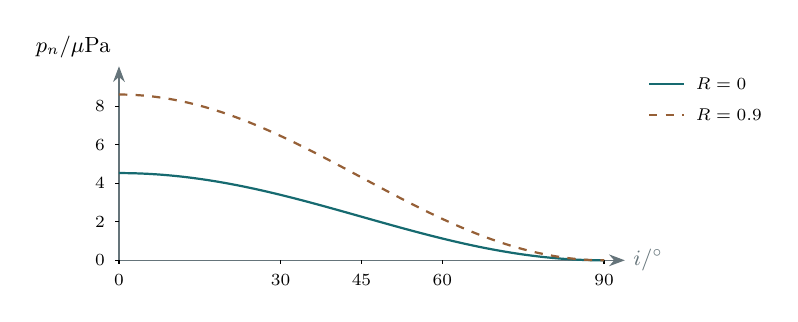
\begin{tikzpicture}[scale=.88,transform shape]
\draw[axis] (0,0.0)--(7.3,0.0) node[right] {$i/{}^\circ$};
\draw[axis] (0,0)--(0,2.8);
\node[above left] at (0,2.8) {$p_n/\mu\mathrm{Pa}$};
\draw[thin] (0.000000,0.0)--(0.000000,-0.06);\node[below,font=\scriptsize] at (0.000000,-0.08) {$ 0 $};
\draw[thin] (2.333333,0.0)--(2.333333,-0.06);\node[below,font=\scriptsize] at (2.333333,-0.08) {$ 30 $};
\draw[thin] (3.500000,0.0)--(3.500000,-0.06);\node[below,font=\scriptsize] at (3.500000,-0.08) {$ 45 $};
\draw[thin] (4.666667,0.0)--(4.666667,-0.06);\node[below,font=\scriptsize] at (4.666667,-0.08) {$ 60 $};
\draw[thin] (7.000000,0.0)--(7.000000,-0.06);\node[below,font=\scriptsize] at (7.000000,-0.08) {$ 90 $};
\draw[thin] (0,0.000000)--(-.06,0.000000);\node[left,font=\scriptsize] at (-.08,0.000000) {$ 0 $};
\draw[thin] (0,0.555556)--(-.06,0.555556);\node[left,font=\scriptsize] at (-.08,0.555556) {$ 2 $};
\draw[thin] (0,1.111111)--(-.06,1.111111);\node[left,font=\scriptsize] at (-.08,1.111111) {$ 4 $};
\draw[thin] (0,1.666667)--(-.06,1.666667);\node[left,font=\scriptsize] at (-.08,1.666667) {$ 6 $};
\draw[thin] (0,2.222222)--(-.06,2.222222);\node[left,font=\scriptsize] at (-.08,2.222222) {$ 8 $};
\draw[thick,color=accent] plot coordinates {(0.0000000,1.2592593) (0.0291667,1.2592053) (0.0583333,1.2590435) (0.0875000,1.2587738) (0.1166667,1.2583964) (0.1458333,1.2579112) (0.1750000,1.2573183) (0.2041667,1.2566179) (0.2333333,1.2558101) (0.2625000,1.2548950) (0.2916667,1.2538727) (0.3208333,1.2527435) (0.3500000,1.2515075) (0.3791667,1.2501649) (0.4083333,1.2487161) (0.4375000,1.2471611) (0.4666667,1.2455003) (0.4958333,1.2437341) (0.5250000,1.2418625) (0.5541667,1.2398861) (0.5833333,1.2378051) (0.6125000,1.2356200) (0.6416667,1.2333309) (0.6708333,1.2309385) (0.7000000,1.2284430) (0.7291667,1.2258449) (0.7583333,1.2231446) (0.7875000,1.2203427) (0.8166667,1.2174395) (0.8458333,1.2144356) (0.8750000,1.2113316) (0.9041667,1.2081278) (0.9333333,1.2048249) (0.9625000,1.2014235) (0.9916667,1.1979241) (1.0208333,1.1943273) (1.0500000,1.1906337) (1.0791667,1.1868441) (1.1083333,1.1829589) (1.1375000,1.1789790) (1.1666667,1.1749049) (1.1958333,1.1707374) (1.2250000,1.1664771) (1.2541667,1.1621249) (1.2833333,1.1576815) (1.3125000,1.1531475) (1.3416667,1.1485239) (1.3708333,1.1438113) (1.4000000,1.1390107) (1.4291667,1.1341228) (1.4583333,1.1291484) (1.4875000,1.1240884) (1.5166667,1.1189438) (1.5458333,1.1137152) (1.5750000,1.1084038) (1.6041667,1.1030102) (1.6333333,1.0975356) (1.6625000,1.0919808) (1.6916667,1.0863468) (1.7208333,1.0806346) (1.7500000,1.0748450) (1.7791667,1.0689792) (1.8083333,1.0630381) (1.8375000,1.0570227) (1.8666667,1.0509341) (1.8958333,1.0447733) (1.9250000,1.0385414) (1.9541667,1.0322394) (1.9833333,1.0258684) (2.0125000,1.0194295) (2.0416667,1.0129239) (2.0708333,1.0063525) (2.1000000,0.9997166) (2.1291667,0.9930173) (2.1583333,0.9862558) (2.1875000,0.9794331) (2.2166667,0.9725505) (2.2458333,0.9656091) (2.2750000,0.9586102) (2.3041667,0.9515549) (2.3333333,0.9444444) (2.3625000,0.9372800) (2.3916667,0.9300629) (2.4208333,0.9227943) (2.4500000,0.9154755) (2.4791667,0.9081077) (2.5083333,0.9006922) (2.5375000,0.8932302) (2.5666667,0.8857231) (2.5958333,0.8781721) (2.6250000,0.8705785) (2.6541667,0.8629436) (2.6833333,0.8552687) (2.7125000,0.8475552) (2.7416667,0.8398043) (2.7708333,0.8320174) (2.8000000,0.8241959) (2.8291667,0.8163410) (2.8583333,0.8084541) (2.8875000,0.8005366) (2.9166667,0.7925898) (2.9458333,0.7846150) (2.9750000,0.7766137) (3.0041667,0.7685873) (3.0333333,0.7605370) (3.0625000,0.7524643) (3.0916667,0.7443705) (3.1208333,0.7362571) (3.1500000,0.7281254) (3.1791667,0.7199768) (3.2083333,0.7118128) (3.2375000,0.7036347) (3.2666667,0.6954438) (3.2958333,0.6872418) (3.3250000,0.6790298) (3.3541667,0.6708094) (3.3833333,0.6625819) (3.4125000,0.6543488) (3.4416667,0.6461114) (3.4708333,0.6378712) (3.5000000,0.6296296) (3.5291667,0.6213880) (3.5583333,0.6131478) (3.5875000,0.6049105) (3.6166667,0.5966774) (3.6458333,0.5884499) (3.6750000,0.5802295) (3.7041667,0.5720175) (3.7333333,0.5638154) (3.7625000,0.5556246) (3.7916667,0.5474465) (3.8208333,0.5392824) (3.8500000,0.5311339) (3.8791667,0.5230022) (3.9083333,0.5148887) (3.9375000,0.5067950) (3.9666667,0.4987223) (3.9958333,0.4906720) (4.0250000,0.4826455) (4.0541667,0.4746442) (4.0833333,0.4666695) (4.1125000,0.4587227) (4.1416667,0.4508052) (4.1708333,0.4429183) (4.2000000,0.4350634) (4.2291667,0.4272418) (4.2583333,0.4194549) (4.2875000,0.4117041) (4.3166667,0.4039906) (4.3458333,0.3963157) (4.3750000,0.3886808) (4.4041667,0.3810872) (4.4333333,0.3735362) (4.4625000,0.3660291) (4.4916667,0.3585671) (4.5208333,0.3511516) (4.5500000,0.3437838) (4.5791667,0.3364649) (4.6083333,0.3291963) (4.6375000,0.3219792) (4.6666667,0.3148148) (4.6958333,0.3077044) (4.7250000,0.3006491) (4.7541667,0.2936501) (4.7833333,0.2867088) (4.8125000,0.2798261) (4.8416667,0.2730035) (4.8708333,0.2662419) (4.9000000,0.2595426) (4.9291667,0.2529067) (4.9583333,0.2463354) (4.9875000,0.2398297) (5.0166667,0.2333909) (5.0458333,0.2270199) (5.0750000,0.2207179) (5.1041667,0.2144860) (5.1333333,0.2083252) (5.1625000,0.2022366) (5.1916667,0.1962212) (5.2208333,0.1902801) (5.2500000,0.1844142) (5.2791667,0.1786247) (5.3083333,0.1729124) (5.3375000,0.1672784) (5.3666667,0.1617236) (5.3958333,0.1562490) (5.4250000,0.1508555) (5.4541667,0.1455440) (5.4833333,0.1403155) (5.5125000,0.1351708) (5.5416667,0.1301109) (5.5708333,0.1251365) (5.6000000,0.1202486) (5.6291667,0.1154479) (5.6583333,0.1107354) (5.6875000,0.1061117) (5.7166667,0.1015778) (5.7458333,0.0971343) (5.7750000,0.0927821) (5.8041667,0.0885219) (5.8333333,0.0843544) (5.8625000,0.0802803) (5.8916667,0.0763003) (5.9208333,0.0724152) (5.9500000,0.0686255) (5.9791667,0.0649320) (6.0083333,0.0613352) (6.0375000,0.0578358) (6.0666667,0.0544343) (6.0958333,0.0511315) (6.1250000,0.0479277) (6.1541667,0.0448236) (6.1833333,0.0418197) (6.2125000,0.0389166) (6.2416667,0.0361146) (6.2708333,0.0334144) (6.3000000,0.0308163) (6.3291667,0.0283208) (6.3583333,0.0259283) (6.3875000,0.0236393) (6.4166667,0.0214541) (6.4458333,0.0193731) (6.4750000,0.0173967) (6.5041667,0.0155252) (6.5333333,0.0137589) (6.5625000,0.0120982) (6.5916667,0.0105432) (6.6208333,0.0090943) (6.6500000,0.0077518) (6.6791667,0.0065158) (6.7083333,0.0053866) (6.7375000,0.0043643) (6.7666667,0.0034492) (6.7958333,0.0026413) (6.8250000,0.0019409) (6.8541667,0.0013481) (6.8833333,0.0008629) (6.9125000,0.0004854) (6.9416667,0.0002158) (6.9708333,0.0000539) (7.0000000,0.0000000)};
\draw[thick,color=accent] (7.65,2.55)--(8.15,2.55);\node[right,font=\scriptsize] at (8.2,2.55) {$R=0$};
\draw[thick,dashed,color=warm] plot coordinates {(0.0000000,2.3925926) (0.0291667,2.3924901) (0.0583333,2.3921827) (0.0875000,2.3916703) (0.1166667,2.3909531) (0.1458333,2.3900312) (0.1750000,2.3889048) (0.2041667,2.3875740) (0.2333333,2.3860392) (0.2625000,2.3843004) (0.2916667,2.3823581) (0.3208333,2.3802126) (0.3500000,2.3778642) (0.3791667,2.3753134) (0.4083333,2.3725605) (0.4375000,2.3696061) (0.4666667,2.3664506) (0.4958333,2.3630947) (0.5250000,2.3595388) (0.5541667,2.3557836) (0.5833333,2.3518298) (0.6125000,2.3476779) (0.6416667,2.3433288) (0.6708333,2.3387831) (0.7000000,2.3340417) (0.7291667,2.3291053) (0.7583333,2.3239748) (0.7875000,2.3186511) (0.8166667,2.3131351) (0.8458333,2.3074277) (0.8750000,2.3015300) (0.9041667,2.2954428) (0.9333333,2.2891673) (0.9625000,2.2827046) (0.9916667,2.2760557) (1.0208333,2.2692218) (1.0500000,2.2622041) (1.0791667,2.2550037) (1.1083333,2.2476220) (1.1375000,2.2400600) (1.1666667,2.2323193) (1.1958333,2.2244010) (1.2250000,2.2163066) (1.2541667,2.2080374) (1.2833333,2.1995948) (1.3125000,2.1909803) (1.3416667,2.1821954) (1.3708333,2.1732416) (1.4000000,2.1641203) (1.4291667,2.1548333) (1.4583333,2.1453820) (1.4875000,2.1357680) (1.5166667,2.1259931) (1.5458333,2.1160589) (1.5750000,2.1059671) (1.6041667,2.0957195) (1.6333333,2.0853177) (1.6625000,2.0747636) (1.6916667,2.0640590) (1.7208333,2.0532057) (1.7500000,2.0422055) (1.7791667,2.0310604) (1.8083333,2.0197723) (1.8375000,2.0083431) (1.8666667,1.9967748) (1.8958333,1.9850693) (1.9250000,1.9732286) (1.9541667,1.9612548) (1.9833333,1.9491499) (2.0125000,1.9369161) (2.0416667,1.9245553) (2.0708333,1.9120698) (2.1000000,1.8994616) (2.1291667,1.8867329) (2.1583333,1.8738860) (2.1875000,1.8609229) (2.2166667,1.8478460) (2.2458333,1.8346574) (2.2750000,1.8213594) (2.3041667,1.8079543) (2.3333333,1.7944444) (2.3625000,1.7808321) (2.3916667,1.7671196) (2.4208333,1.7533092) (2.4500000,1.7394034) (2.4791667,1.7254046) (2.5083333,1.7113151) (2.5375000,1.6971374) (2.5666667,1.6828738) (2.5958333,1.6685269) (2.6250000,1.6540991) (2.6541667,1.6395928) (2.6833333,1.6250105) (2.7125000,1.6103548) (2.7416667,1.5956282) (2.7708333,1.5808331) (2.8000000,1.5659722) (2.8291667,1.5510479) (2.8583333,1.5360628) (2.8875000,1.5210195) (2.9166667,1.5059206) (2.9458333,1.4907686) (2.9750000,1.4755661) (3.0041667,1.4603158) (3.0333333,1.4450203) (3.0625000,1.4296821) (3.0916667,1.4143040) (3.1208333,1.3988885) (3.1500000,1.3834383) (3.1791667,1.3679560) (3.2083333,1.3524443) (3.2375000,1.3369058) (3.2666667,1.3213433) (3.2958333,1.3057593) (3.3250000,1.2901566) (3.3541667,1.2745378) (3.3833333,1.2589056) (3.4125000,1.2432627) (3.4416667,1.2276117) (3.4708333,1.2119553) (3.5000000,1.1962963) (3.5291667,1.1806373) (3.5583333,1.1649809) (3.5875000,1.1493299) (3.6166667,1.1336870) (3.6458333,1.1180548) (3.6750000,1.1024360) (3.7041667,1.0868332) (3.7333333,1.0712493) (3.7625000,1.0556867) (3.7916667,1.0401483) (3.8208333,1.0246366) (3.8500000,1.0091543) (3.8791667,0.9937041) (3.9083333,0.9782886) (3.9375000,0.9629105) (3.9666667,0.9475723) (3.9958333,0.9322768) (4.0250000,0.9170265) (4.0541667,0.9018240) (4.0833333,0.8866720) (4.1125000,0.8715731) (4.1416667,0.8565298) (4.1708333,0.8415447) (4.2000000,0.8266204) (4.2291667,0.8117595) (4.2583333,0.7969644) (4.2875000,0.7822377) (4.3166667,0.7675820) (4.3458333,0.7529998) (4.3750000,0.7384935) (4.4041667,0.7240657) (4.4333333,0.7097188) (4.4625000,0.6954552) (4.4916667,0.6812775) (4.5208333,0.6671880) (4.5500000,0.6531891) (4.5791667,0.6392834) (4.6083333,0.6254730) (4.6375000,0.6117605) (4.6666667,0.5981481) (4.6958333,0.5846383) (4.7250000,0.5712332) (4.7541667,0.5579352) (4.7833333,0.5447466) (4.8125000,0.5316697) (4.8416667,0.5187066) (4.8708333,0.5058596) (4.9000000,0.4931310) (4.9291667,0.4805228) (4.9583333,0.4680373) (4.9875000,0.4556765) (5.0166667,0.4434426) (5.0458333,0.4313378) (5.0750000,0.4193640) (5.1041667,0.4075233) (5.1333333,0.3958178) (5.1625000,0.3842495) (5.1916667,0.3728203) (5.2208333,0.3615322) (5.2500000,0.3503871) (5.2791667,0.3393869) (5.3083333,0.3285336) (5.3375000,0.3178290) (5.3666667,0.3072749) (5.3958333,0.2968731) (5.4250000,0.2866255) (5.4541667,0.2765337) (5.4833333,0.2665995) (5.5125000,0.2568246) (5.5416667,0.2472106) (5.5708333,0.2377593) (5.6000000,0.2284723) (5.6291667,0.2193510) (5.6583333,0.2103972) (5.6875000,0.2016123) (5.7166667,0.1929978) (5.7458333,0.1845552) (5.7750000,0.1762860) (5.8041667,0.1681916) (5.8333333,0.1602733) (5.8625000,0.1525326) (5.8916667,0.1449706) (5.9208333,0.1375889) (5.9500000,0.1303885) (5.9791667,0.1233708) (6.0083333,0.1165369) (6.0375000,0.1098880) (6.0666667,0.1034252) (6.0958333,0.0971498) (6.1250000,0.0910626) (6.1541667,0.0851649) (6.1833333,0.0794575) (6.2125000,0.0739415) (6.2416667,0.0686178) (6.2708333,0.0634873) (6.3000000,0.0585509) (6.3291667,0.0538095) (6.3583333,0.0492638) (6.3875000,0.0449147) (6.4166667,0.0407628) (6.4458333,0.0368089) (6.4750000,0.0330538) (6.5041667,0.0294979) (6.5333333,0.0261419) (6.5625000,0.0229865) (6.5916667,0.0200321) (6.6208333,0.0172792) (6.6500000,0.0147284) (6.6791667,0.0123800) (6.7083333,0.0102345) (6.7375000,0.0082922) (6.7666667,0.0065534) (6.7958333,0.0050185) (6.8250000,0.0036878) (6.8541667,0.0025614) (6.8833333,0.0016395) (6.9125000,0.0009223) (6.9416667,0.0004099) (6.9708333,0.0001025) (7.0000000,0.0000000)};
\draw[thick,dashed,color=warm] (7.65,2.0999999999999996)--(8.15,2.0999999999999996);\node[right,font=\scriptsize] at (8.2,2.0999999999999996) {$R=0.9$};
\end{tikzpicture}
\figcaption{变图近1.1V6\quad 1360瓦每平方米光束给微帕量级的法向压力}
\end{minipage}\end{center}
\item \textbf{光子计数的法向力涨落。}单频光子命中为Poisson过程，面积$S$、平均功率$IS\cos i$、平均时间窗$\Delta t$。求窗内平均法向力的方差。

单个命中光子以概率$1-R$给法向冲量$(h\nu/c)\cos i$，以概率$R$给其两倍。记平均命中数为$\lambda=IS\cos i\,\Delta t/(h\nu)$，单次冲量为$q_n$，则$\langle q_n\rangle=(h\nu/c)(1+R)\cos i$、$\langle q_n^2\rangle=(h\nu/c)^2(1+3R)\cos^2i$。给定命中数$N$时，冲量和的条件方差为$N\operatorname{Var}(q_n)$；再计Poisson计数的$\operatorname{Var}(N)=\lambda$，总方差为$\lambda\operatorname{Var}(q_n)+\lambda\langle q_n\rangle^2=\lambda\langle q_n^2\rangle$。除以$\Delta t^2$得到平均力的方差，故
\[
 \operatorname{Var}(\bar F_n)
 =\frac{IS\,h\nu}{c^2\Delta t}(1+3R)\cos^3i.
\]
除以$\langle F_n\rangle^2$，得相对方差$[h\nu/(IS\Delta t\cos i)](1+3R)/(1+R)^2$。变图近1.1V7画反射率系数，它在$R=1/3$为$9/8$，两端为1；观测窗越长，平均力的统计起伏越小。
\begin{center}\begin{minipage}{.98\linewidth}\centering
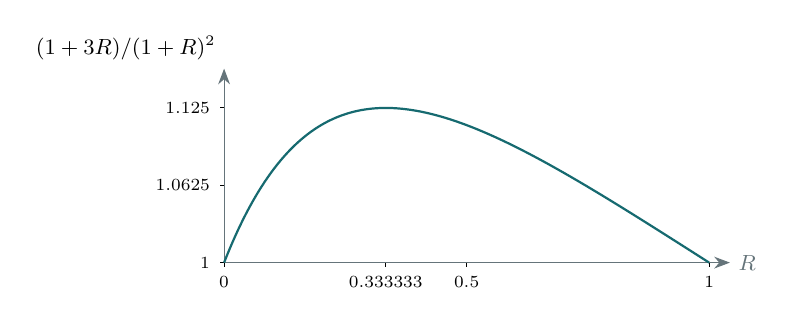
\begin{tikzpicture}[scale=.88,transform shape]
\draw[axis] (0,0)--(7.3,0) node[right] {$R$};
\draw[axis] (0,0)--(0,2.8);
\node[above left] at (0,2.8) {$(1+3R)/(1+R)^2$};
\draw[thin] (0.000000,0)--(0.000000,-0.06);\node[below,font=\scriptsize] at (0.000000,-0.08) {$ 0 $};
\draw[thin] (2.333333,0)--(2.333333,-0.06);\node[below,font=\scriptsize] at (2.333333,-0.08) {$ 0.333333 $};
\draw[thin] (3.500000,0)--(3.500000,-0.06);\node[below,font=\scriptsize] at (3.500000,-0.08) {$ 0.5 $};
\draw[thin] (7.000000,0)--(7.000000,-0.06);\node[below,font=\scriptsize] at (7.000000,-0.08) {$ 1 $};
\draw[thin] (0,0.000000)--(-.06,0.000000);\node[left,font=\scriptsize] at (-.08,0.000000) {$ 1 $};
\draw[thin] (0,1.116071)--(-.06,1.116071);\node[left,font=\scriptsize] at (-.08,1.116071) {$ 1.0625 $};
\draw[thin] (0,2.232143)--(-.06,2.232143);\node[left,font=\scriptsize] at (-.08,2.232143) {$ 1.125 $};
\draw[thick,color=accent] plot coordinates {(0.0000000,0.0000000) (0.0291667,0.0734811) (0.0583333,0.1451404) (0.0875000,0.2150151) (0.1166667,0.2831420) (0.1458333,0.3495567) (0.1750000,0.4142942) (0.2041667,0.4773886) (0.2333333,0.5388732) (0.2625000,0.5987807) (0.2916667,0.6571429) (0.3208333,0.7139909) (0.3500000,0.7693554) (0.3791667,0.8232659) (0.4083333,0.8757518) (0.4375000,0.9268413) (0.4666667,0.9765625) (0.4958333,1.0249425) (0.5250000,1.0720080) (0.5541667,1.1177851) (0.5833333,1.1622992) (0.6125000,1.2055754) (0.6416667,1.2476379) (0.6708333,1.2885107) (0.7000000,1.3282172) (0.7291667,1.3667802) (0.7583333,1.4042222) (0.7875000,1.4405649) (0.8166667,1.4758298) (0.8458333,1.5100380) (0.8750000,1.5432099) (0.9041667,1.5753656) (0.9333333,1.6065250) (0.9625000,1.6367071) (0.9916667,1.6659309) (1.0208333,1.6942149) (1.0500000,1.7215771) (1.0791667,1.7480353) (1.1083333,1.7736068) (1.1375000,1.7983086) (1.1666667,1.8221574) (1.1958333,1.8451695) (1.2250000,1.8673608) (1.2541667,1.8887470) (1.2833333,1.9093434) (1.3125000,1.9291650) (1.3416667,1.9482266) (1.3708333,1.9665425) (1.4000000,1.9841270) (1.4291667,2.0009938) (1.4583333,2.0171564) (1.4875000,2.0326283) (1.5166667,2.0474225) (1.5458333,2.0615516) (1.5750000,2.0750283) (1.6041667,2.0878647) (1.6333333,2.1000730) (1.6625000,2.1116650) (1.6916667,2.1226521) (1.7208333,2.1330458) (1.7500000,2.1428571) (1.7791667,2.1520970) (1.8083333,2.1607762) (1.8375000,2.1689050) (1.8666667,2.1764939) (1.8958333,2.1835528) (1.9250000,2.1900917) (1.9541667,2.1961203) (1.9833333,2.2016481) (2.0125000,2.2066844) (2.0416667,2.2112383) (2.0708333,2.2153189) (2.1000000,2.2189349) (2.1291667,2.2220950) (2.1583333,2.2248077) (2.1875000,2.2270813) (2.2166667,2.2289239) (2.2458333,2.2303436) (2.2750000,2.2313482) (2.3041667,2.2319454) (2.3333333,2.2321429) (2.3625000,2.2319479) (2.3916667,2.2313678) (2.4208333,2.2304098) (2.4500000,2.2290809) (2.4791667,2.2273880) (2.5083333,2.2253378) (2.5375000,2.2229370) (2.5666667,2.2201921) (2.5958333,2.2171094) (2.6250000,2.2136954) (2.6541667,2.2099561) (2.6833333,2.2058976) (2.7125000,2.2015259) (2.7416667,2.1968467) (2.7708333,2.1918658) (2.8000000,2.1865889) (2.8291667,2.1810215) (2.8583333,2.1751689) (2.8875000,2.1690366) (2.9166667,2.1626298) (2.9458333,2.1559535) (2.9750000,2.1490129) (3.0041667,2.1418129) (3.0333333,2.1343583) (3.0625000,2.1266541) (3.0916667,2.1187047) (3.1208333,2.1105150) (3.1500000,2.1020893) (3.1791667,2.0934323) (3.2083333,2.0845481) (3.2375000,2.0754412) (3.2666667,2.0661157) (3.2958333,2.0565758) (3.3250000,2.0468256) (3.3541667,2.0368691) (3.3833333,2.0267102) (3.4125000,2.0163528) (3.4416667,2.0058006) (3.4708333,1.9950575) (3.5000000,1.9841270) (3.5291667,1.9730128) (3.5583333,1.9617184) (3.5875000,1.9502473) (3.6166667,1.9386030) (3.6458333,1.9267887) (3.6750000,1.9148078) (3.7041667,1.9026636) (3.7333333,1.8903592) (3.7625000,1.8778977) (3.7916667,1.8652823) (3.8208333,1.8525159) (3.8500000,1.8396016) (3.8791667,1.8265423) (3.9083333,1.8133408) (3.9375000,1.8000000) (3.9666667,1.7865227) (3.9958333,1.7729115) (4.0250000,1.7591693) (4.0541667,1.7452985) (4.0833333,1.7313019) (4.1125000,1.7171820) (4.1416667,1.7029413) (4.1708333,1.6885822) (4.2000000,1.6741071) (4.2291667,1.6595186) (4.2583333,1.6448188) (4.2875000,1.6300102) (4.3166667,1.6150950) (4.3458333,1.6000753) (4.3750000,1.5849535) (4.4041667,1.5697316) (4.4333333,1.5544119) (4.4625000,1.5389962) (4.4916667,1.5234868) (4.5208333,1.5078856) (4.5500000,1.4921947) (4.5791667,1.4764159) (4.6083333,1.4605511) (4.6375000,1.4446024) (4.6666667,1.4285714) (4.6958333,1.4124601) (4.7250000,1.3962702) (4.7541667,1.3800036) (4.7833333,1.3636618) (4.8125000,1.3472467) (4.8416667,1.3307599) (4.8708333,1.3142031) (4.9000000,1.2975779) (4.9291667,1.2808858) (4.9583333,1.2641285) (4.9875000,1.2473075) (5.0166667,1.2304243) (5.0458333,1.2134804) (5.0750000,1.1964773) (5.1041667,1.1794165) (5.1333333,1.1622992) (5.1625000,1.1451271) (5.1916667,1.1279013) (5.2208333,1.1106233) (5.2500000,1.0932945) (5.2791667,1.0759160) (5.3083333,1.0584893) (5.3375000,1.0410155) (5.3666667,1.0234959) (5.3958333,1.0059318) (5.4250000,0.9883243) (5.4541667,0.9706747) (5.4833333,0.9529840) (5.5125000,0.9352536) (5.5416667,0.9174844) (5.5708333,0.8996775) (5.6000000,0.8818342) (5.6291667,0.8639554) (5.6583333,0.8460423) (5.6875000,0.8280958) (5.7166667,0.8101170) (5.7458333,0.7921069) (5.7750000,0.7740664) (5.8041667,0.7559966) (5.8333333,0.7378985) (5.8625000,0.7197728) (5.8916667,0.7016207) (5.9208333,0.6834430) (5.9500000,0.6652405) (5.9791667,0.6470143) (6.0083333,0.6287650) (6.0375000,0.6104937) (6.0666667,0.5922012) (6.0958333,0.5738882) (6.1250000,0.5555556) (6.1541667,0.5372041) (6.1833333,0.5188347) (6.2125000,0.5004480) (6.2416667,0.4820448) (6.2708333,0.4636259) (6.3000000,0.4451919) (6.3291667,0.4267437) (6.3583333,0.4082820) (6.3875000,0.3898073) (6.4166667,0.3713206) (6.4458333,0.3528223) (6.4750000,0.3343132) (6.5041667,0.3157939) (6.5333333,0.2972652) (6.5625000,0.2787275) (6.5916667,0.2601816) (6.6208333,0.2416281) (6.6500000,0.2230675) (6.6791667,0.2045005) (6.7083333,0.1859277) (6.7375000,0.1673496) (6.7666667,0.1487668) (6.7958333,0.1301798) (6.8250000,0.1115893) (6.8541667,0.0929956) (6.8833333,0.0743995) (6.9125000,0.0558014) (6.9416667,0.0372017) (6.9708333,0.0186011) (7.0000000,0.0000000)};
\end{tikzpicture}
\figcaption{变图近1.1V7\quad Poisson命中与两种冲量的二阶矩给相对涨落系数}
\end{minipage}\end{center}
\item \textbf{以入射轴分解总力。}控制截获总功率$P$固定，求力在入射方向及垂直入射方向的分量，找横向分量的最大值。

令$\hat{\boldsymbol u}=-\sin i\,\hat{\boldsymbol n}+\cos i\,\hat{\boldsymbol t}$，它垂直$\hat{\boldsymbol k}_i$。主解矢量式给
\[
 F_\parallel=\frac Pc(1+R\cos2i),\qquad
 F_u=-\frac{RP}{c}\sin2i.
\]
这里$\hat{\boldsymbol k}_i\cdot\hat{\boldsymbol k}_r=-\cos2i$。故$|F_u|$在45度最大，为$RP/c$。变图近1.1V8取$R=1/2$画这两种按$P/c$归一化的分量；受控截获功率固定时，倾角改变由出射方向决定的动量差。
\begin{center}\begin{minipage}{.98\linewidth}\centering
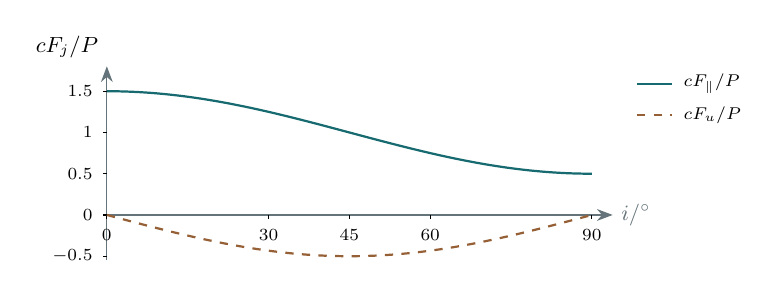
\begin{tikzpicture}[scale=.88,transform shape]
\draw[axis] (0,0.6547619047619048)--(7.3,0.6547619047619048) node[right] {$i/{}^\circ$};
\draw[axis] (0,0)--(0,2.8);
\node[above left] at (0,2.8) {$cF_j/P$};
\draw[thin] (0.000000,0.6547619047619048)--(0.000000,0.5947619047619048);\node[below,font=\scriptsize] at (0.000000,0.5747619047619048) {$ 0 $};
\draw[thin] (2.333333,0.6547619047619048)--(2.333333,0.5947619047619048);\node[below,font=\scriptsize] at (2.333333,0.5747619047619048) {$ 30 $};
\draw[thin] (3.500000,0.6547619047619048)--(3.500000,0.5947619047619048);\node[below,font=\scriptsize] at (3.500000,0.5747619047619048) {$ 45 $};
\draw[thin] (4.666667,0.6547619047619048)--(4.666667,0.5947619047619048);\node[below,font=\scriptsize] at (4.666667,0.5747619047619048) {$ 60 $};
\draw[thin] (7.000000,0.6547619047619048)--(7.000000,0.5947619047619048);\node[below,font=\scriptsize] at (7.000000,0.5747619047619048) {$ 90 $};
\draw[thin] (0,0.059524)--(-.06,0.059524);\node[left,font=\scriptsize] at (-.08,0.059524) {$ -0.5 $};
\draw[thin] (0,0.654762)--(-.06,0.654762);\node[left,font=\scriptsize] at (-.08,0.654762) {$ 0 $};
\draw[thin] (0,1.250000)--(-.06,1.250000);\node[left,font=\scriptsize] at (-.08,1.250000) {$ 0.5 $};
\draw[thin] (0,1.845238)--(-.06,1.845238);\node[left,font=\scriptsize] at (-.08,1.845238) {$ 1 $};
\draw[thin] (0,2.440476)--(-.06,2.440476);\node[left,font=\scriptsize] at (-.08,2.440476) {$ 1.5 $};
\draw[thick,color=accent] plot coordinates {(0.0000000,2.4404762) (0.0291667,2.4404252) (0.0583333,2.4402722) (0.0875000,2.4400173) (0.1166667,2.4396604) (0.1458333,2.4392017) (0.1750000,2.4386413) (0.2041667,2.4379791) (0.2333333,2.4372154) (0.2625000,2.4363503) (0.2916667,2.4353838) (0.3208333,2.4343163) (0.3500000,2.4331478) (0.3791667,2.4318786) (0.4083333,2.4305089) (0.4375000,2.4290389) (0.4666667,2.4274688) (0.4958333,2.4257990) (0.5250000,2.4240297) (0.5541667,2.4221613) (0.5833333,2.4201939) (0.6125000,2.4181281) (0.6416667,2.4159641) (0.6708333,2.4137023) (0.7000000,2.4113432) (0.7291667,2.4088870) (0.7583333,2.4063342) (0.7875000,2.4036853) (0.8166667,2.4009407) (0.8458333,2.3981009) (0.8750000,2.3951664) (0.9041667,2.3921376) (0.9333333,2.3890152) (0.9625000,2.3857995) (0.9916667,2.3824912) (1.0208333,2.3790909) (1.0500000,2.3755991) (1.0791667,2.3720165) (1.1083333,2.3683435) (1.1375000,2.3645810) (1.1666667,2.3607294) (1.1958333,2.3567895) (1.2250000,2.3527620) (1.2541667,2.3486475) (1.2833333,2.3444468) (1.3125000,2.3401605) (1.3416667,2.3357894) (1.3708333,2.3313343) (1.4000000,2.3267958) (1.4291667,2.3221749) (1.4583333,2.3174722) (1.4875000,2.3126886) (1.5166667,2.3078250) (1.5458333,2.3028820) (1.5750000,2.2978607) (1.6041667,2.2927618) (1.6333333,2.2875862) (1.6625000,2.2823348) (1.6916667,2.2770086) (1.7208333,2.2716083) (1.7500000,2.2661350) (1.7791667,2.2605896) (1.8083333,2.2549730) (1.8375000,2.2492862) (1.8666667,2.2435301) (1.8958333,2.2377058) (1.9250000,2.2318143) (1.9541667,2.2258565) (1.9833333,2.2198336) (2.0125000,2.2137464) (2.0416667,2.2075961) (2.0708333,2.2013837) (2.1000000,2.1951103) (2.1291667,2.1887769) (2.1583333,2.1823847) (2.1875000,2.1759347) (2.2166667,2.1694280) (2.2458333,2.1628658) (2.2750000,2.1562491) (2.3041667,2.1495792) (2.3333333,2.1428571) (2.3625000,2.1360841) (2.3916667,2.1292612) (2.4208333,2.1223896) (2.4500000,2.1154705) (2.4791667,2.1085052) (2.5083333,2.1014947) (2.5375000,2.0944403) (2.5666667,2.0873432) (2.5958333,2.0802047) (2.6250000,2.0730259) (2.6541667,2.0658080) (2.6833333,2.0585524) (2.7125000,2.0512602) (2.7416667,2.0439327) (2.7708333,2.0365711) (2.8000000,2.0291768) (2.8291667,2.0217509) (2.8583333,2.0142948) (2.8875000,2.0068098) (2.9166667,1.9992971) (2.9458333,1.9917579) (2.9750000,1.9841937) (3.0041667,1.9766056) (3.0333333,1.9689951) (3.0625000,1.9613633) (3.0916667,1.9537116) (3.1208333,1.9460414) (3.1500000,1.9383538) (3.1791667,1.9306504) (3.2083333,1.9229323) (3.2375000,1.9152008) (3.2666667,1.9074574) (3.2958333,1.8997033) (3.3250000,1.8919399) (3.3541667,1.8841685) (3.3833333,1.8763905) (3.4125000,1.8686070) (3.4416667,1.8608196) (3.4708333,1.8530295) (3.5000000,1.8452381) (3.5291667,1.8374467) (3.5583333,1.8296566) (3.5875000,1.8218692) (3.6166667,1.8140857) (3.6458333,1.8063077) (3.6750000,1.7985363) (3.7041667,1.7907728) (3.7333333,1.7830188) (3.7625000,1.7752754) (3.7916667,1.7675439) (3.8208333,1.7598258) (3.8500000,1.7521223) (3.8791667,1.7444348) (3.9083333,1.7367646) (3.9375000,1.7291129) (3.9666667,1.7214811) (3.9958333,1.7138706) (4.0250000,1.7062825) (4.0541667,1.6987183) (4.0833333,1.6911791) (4.1125000,1.6836664) (4.1416667,1.6761813) (4.1708333,1.6687253) (4.2000000,1.6612994) (4.2291667,1.6539051) (4.2583333,1.6465435) (4.2875000,1.6392160) (4.3166667,1.6319238) (4.3458333,1.6246682) (4.3750000,1.6174503) (4.4041667,1.6102715) (4.4333333,1.6031330) (4.4625000,1.5960359) (4.4916667,1.5889815) (4.5208333,1.5819710) (4.5500000,1.5750057) (4.5791667,1.5680866) (4.6083333,1.5612150) (4.6375000,1.5543921) (4.6666667,1.5476190) (4.6958333,1.5408970) (4.7250000,1.5342270) (4.7541667,1.5276104) (4.7833333,1.5210482) (4.8125000,1.5145415) (4.8416667,1.5080915) (4.8708333,1.5016993) (4.9000000,1.4953659) (4.9291667,1.4890925) (4.9583333,1.4828801) (4.9875000,1.4767298) (5.0166667,1.4706426) (5.0458333,1.4646196) (5.0750000,1.4586619) (5.1041667,1.4527703) (5.1333333,1.4469461) (5.1625000,1.4411900) (5.1916667,1.4355032) (5.2208333,1.4298866) (5.2500000,1.4243412) (5.2791667,1.4188679) (5.3083333,1.4134676) (5.3375000,1.4081414) (5.3666667,1.4028900) (5.3958333,1.3977144) (5.4250000,1.3926155) (5.4541667,1.3875941) (5.4833333,1.3826512) (5.5125000,1.3777875) (5.5416667,1.3730040) (5.5708333,1.3683013) (5.6000000,1.3636804) (5.6291667,1.3591419) (5.6583333,1.3546868) (5.6875000,1.3503157) (5.7166667,1.3460294) (5.7458333,1.3418287) (5.7750000,1.3377142) (5.8041667,1.3336867) (5.8333333,1.3297468) (5.8625000,1.3258952) (5.8916667,1.3221327) (5.9208333,1.3184597) (5.9500000,1.3148771) (5.9791667,1.3113853) (6.0083333,1.3079849) (6.0375000,1.3046767) (6.0666667,1.3014610) (6.0958333,1.2983386) (6.1250000,1.2953098) (6.1541667,1.2923753) (6.1833333,1.2895355) (6.2125000,1.2867909) (6.2416667,1.2841420) (6.2708333,1.2815892) (6.3000000,1.2791330) (6.3291667,1.2767738) (6.3583333,1.2745121) (6.3875000,1.2723481) (6.4166667,1.2702822) (6.4458333,1.2683149) (6.4750000,1.2664465) (6.5041667,1.2646772) (6.5333333,1.2630074) (6.5625000,1.2614373) (6.5916667,1.2599673) (6.6208333,1.2585976) (6.6500000,1.2573284) (6.6791667,1.2561599) (6.7083333,1.2550923) (6.7375000,1.2541259) (6.7666667,1.2532608) (6.7958333,1.2524971) (6.8250000,1.2518349) (6.8541667,1.2512745) (6.8833333,1.2508158) (6.9125000,1.2504589) (6.9416667,1.2502040) (6.9708333,1.2500510) (7.0000000,1.2500000)};
\draw[thick,color=accent] (7.65,2.55)--(8.15,2.55);\node[right,font=\scriptsize] at (8.2,2.55) {$cF_\parallel/P$};
\draw[thick,dashed,color=warm] plot coordinates {(0.0000000,0.6547619) (0.0291667,0.6469705) (0.0583333,0.6391804) (0.0875000,0.6313930) (0.1166667,0.6236095) (0.1458333,0.6158315) (0.1750000,0.6080601) (0.2041667,0.6002967) (0.2333333,0.5925426) (0.2625000,0.5847992) (0.2916667,0.5770677) (0.3208333,0.5693496) (0.3500000,0.5616462) (0.3791667,0.5539586) (0.4083333,0.5462884) (0.4375000,0.5386367) (0.4666667,0.5310049) (0.4958333,0.5233944) (0.5250000,0.5158063) (0.5541667,0.5082421) (0.5833333,0.5007029) (0.6125000,0.4931902) (0.6416667,0.4857052) (0.6708333,0.4782491) (0.7000000,0.4708232) (0.7291667,0.4634289) (0.7583333,0.4560673) (0.7875000,0.4487398) (0.8166667,0.4414476) (0.8458333,0.4341920) (0.8750000,0.4269741) (0.9041667,0.4197953) (0.9333333,0.4126568) (0.9625000,0.4055597) (0.9916667,0.3985053) (1.0208333,0.3914948) (1.0500000,0.3845295) (1.0791667,0.3776104) (1.1083333,0.3707388) (1.1375000,0.3639159) (1.1666667,0.3571429) (1.1958333,0.3504208) (1.2250000,0.3437509) (1.2541667,0.3371342) (1.2833333,0.3305720) (1.3125000,0.3240653) (1.3416667,0.3176153) (1.3708333,0.3112231) (1.4000000,0.3048897) (1.4291667,0.2986163) (1.4583333,0.2924039) (1.4875000,0.2862536) (1.5166667,0.2801664) (1.5458333,0.2741435) (1.5750000,0.2681857) (1.6041667,0.2622942) (1.6333333,0.2564699) (1.6625000,0.2507138) (1.6916667,0.2450270) (1.7208333,0.2394104) (1.7500000,0.2338650) (1.7791667,0.2283917) (1.8083333,0.2229914) (1.8375000,0.2176652) (1.8666667,0.2124138) (1.8958333,0.2072382) (1.9250000,0.2021393) (1.9541667,0.1971180) (1.9833333,0.1921750) (2.0125000,0.1873114) (2.0416667,0.1825278) (2.0708333,0.1778251) (2.1000000,0.1732042) (2.1291667,0.1686657) (2.1583333,0.1642106) (2.1875000,0.1598395) (2.2166667,0.1555532) (2.2458333,0.1513525) (2.2750000,0.1472380) (2.3041667,0.1432105) (2.3333333,0.1392706) (2.3625000,0.1354190) (2.3916667,0.1316565) (2.4208333,0.1279835) (2.4500000,0.1244009) (2.4791667,0.1209091) (2.5083333,0.1175088) (2.5375000,0.1142005) (2.5666667,0.1109848) (2.5958333,0.1078624) (2.6250000,0.1048336) (2.6541667,0.1018991) (2.6833333,0.0990593) (2.7125000,0.0963147) (2.7416667,0.0936658) (2.7708333,0.0911130) (2.8000000,0.0886568) (2.8291667,0.0862977) (2.8583333,0.0840359) (2.8875000,0.0818719) (2.9166667,0.0798061) (2.9458333,0.0778387) (2.9750000,0.0759703) (3.0041667,0.0742010) (3.0333333,0.0725312) (3.0625000,0.0709611) (3.0916667,0.0694911) (3.1208333,0.0681214) (3.1500000,0.0668522) (3.1791667,0.0656837) (3.2083333,0.0646162) (3.2375000,0.0636497) (3.2666667,0.0627846) (3.2958333,0.0620209) (3.3250000,0.0613587) (3.3541667,0.0607983) (3.3833333,0.0603396) (3.4125000,0.0599827) (3.4416667,0.0597278) (3.4708333,0.0595748) (3.5000000,0.0595238) (3.5291667,0.0595748) (3.5583333,0.0597278) (3.5875000,0.0599827) (3.6166667,0.0603396) (3.6458333,0.0607983) (3.6750000,0.0613587) (3.7041667,0.0620209) (3.7333333,0.0627846) (3.7625000,0.0636497) (3.7916667,0.0646162) (3.8208333,0.0656837) (3.8500000,0.0668522) (3.8791667,0.0681214) (3.9083333,0.0694911) (3.9375000,0.0709611) (3.9666667,0.0725312) (3.9958333,0.0742010) (4.0250000,0.0759703) (4.0541667,0.0778387) (4.0833333,0.0798061) (4.1125000,0.0818719) (4.1416667,0.0840359) (4.1708333,0.0862977) (4.2000000,0.0886568) (4.2291667,0.0911130) (4.2583333,0.0936658) (4.2875000,0.0963147) (4.3166667,0.0990593) (4.3458333,0.1018991) (4.3750000,0.1048336) (4.4041667,0.1078624) (4.4333333,0.1109848) (4.4625000,0.1142005) (4.4916667,0.1175088) (4.5208333,0.1209091) (4.5500000,0.1244009) (4.5791667,0.1279835) (4.6083333,0.1316565) (4.6375000,0.1354190) (4.6666667,0.1392706) (4.6958333,0.1432105) (4.7250000,0.1472380) (4.7541667,0.1513525) (4.7833333,0.1555532) (4.8125000,0.1598395) (4.8416667,0.1642106) (4.8708333,0.1686657) (4.9000000,0.1732042) (4.9291667,0.1778251) (4.9583333,0.1825278) (4.9875000,0.1873114) (5.0166667,0.1921750) (5.0458333,0.1971180) (5.0750000,0.2021393) (5.1041667,0.2072382) (5.1333333,0.2124138) (5.1625000,0.2176652) (5.1916667,0.2229914) (5.2208333,0.2283917) (5.2500000,0.2338650) (5.2791667,0.2394104) (5.3083333,0.2450270) (5.3375000,0.2507138) (5.3666667,0.2564699) (5.3958333,0.2622942) (5.4250000,0.2681857) (5.4541667,0.2741435) (5.4833333,0.2801664) (5.5125000,0.2862536) (5.5416667,0.2924039) (5.5708333,0.2986163) (5.6000000,0.3048897) (5.6291667,0.3112231) (5.6583333,0.3176153) (5.6875000,0.3240653) (5.7166667,0.3305720) (5.7458333,0.3371342) (5.7750000,0.3437509) (5.8041667,0.3504208) (5.8333333,0.3571429) (5.8625000,0.3639159) (5.8916667,0.3707388) (5.9208333,0.3776104) (5.9500000,0.3845295) (5.9791667,0.3914948) (6.0083333,0.3985053) (6.0375000,0.4055597) (6.0666667,0.4126568) (6.0958333,0.4197953) (6.1250000,0.4269741) (6.1541667,0.4341920) (6.1833333,0.4414476) (6.2125000,0.4487398) (6.2416667,0.4560673) (6.2708333,0.4634289) (6.3000000,0.4708232) (6.3291667,0.4782491) (6.3583333,0.4857052) (6.3875000,0.4931902) (6.4166667,0.5007029) (6.4458333,0.5082421) (6.4750000,0.5158063) (6.5041667,0.5233944) (6.5333333,0.5310049) (6.5625000,0.5386367) (6.5916667,0.5462884) (6.6208333,0.5539586) (6.6500000,0.5616462) (6.6791667,0.5693496) (6.7083333,0.5770677) (6.7375000,0.5847992) (6.7666667,0.5925426) (6.7958333,0.6002967) (6.8250000,0.6080601) (6.8541667,0.6158315) (6.8833333,0.6236095) (6.9125000,0.6313930) (6.9416667,0.6391804) (6.9708333,0.6469705) (7.0000000,0.6547619)};
\draw[thick,dashed,color=warm] (7.65,2.0999999999999996)--(8.15,2.0999999999999996);\node[right,font=\scriptsize] at (8.2,2.0999999999999996) {$cF_u/P$};
\end{tikzpicture}
\figcaption{变图近1.1V8\quad 固定截获功率P时按入射轴分解合力}
\end{minipage}\end{center}
\end{enumerate}

\Needspace{13\baselineskip}

\pdfbookmark[2]{第 2 题 非均匀激光束中的微棱镜}{q2}

\section*{第 2 题\quad 非均匀激光束中的微棱镜}\label{q:2}

很小的等腰玻璃三棱镜顶角为$A=\pi-2\alpha$，竖直底边长$2h$，沿$z$的厚度为$w$，折射率$n$、密度$\rho$。顶点朝向从左沿$+x$传播的激光，三角形端面平行$xy$，底面平行$yz$，保持取向不转动；各面理想减反射。激光沿$z$均匀，沿$y$有
\[
I(y)=I_0\left(1-\frac{|y|}{4h}\right)\quad(|y|\leqslant4h),
\]
其他位置为零。棱镜尖端位于$y=y_0$，$|y_0|\leqslant3h$，忽略光强随$x$改变和运动的多普勒修正。
\begin{enumerate}[label=（\arabic*）]
\item 求进入上斜面、由竖直底面射出光线的向下偏转角$\theta$。
\item 计算光给棱镜的$F_x,F_y$，并画随$y_0$变化的曲线。
\item 取$\alpha=30^\circ,h=10\,\mu\mathrm m,n=1.5,w=1\,\mathrm{mm},\rho=2.5\times10^3\,\mathrm{kg/m^3}$。激光全宽为$80\,\mu\mathrm m$、$z$宽1mm，棱镜在$y_0=-h/2$，求使竖直光力平衡重力所需的光束总功率。取$g=9.8\,\mathrm{m/s^2},c=3.00\times10^8\,\mathrm{m/s}$，说明水平方向的条件。
\item 无重力时，取$I_0=10^8\,\mathrm{W/m^2}$，从$y_0=h/20$静止释放，求竖直小振动周期。水平光力另由约束平衡。
\end{enumerate}

\begin{center}\begin{minipage}{.98\linewidth}\centering
\begin{tikzpicture}[scale=.9,transform shape]
\draw[object] (0.00000,0.00000)--(0.98150,1.70000)--(0.98150,-1.70000)--(0.00000,0.00000);\draw[<->,thin,color=muted] (1.48150,-1.70000)--(1.48150,1.70000);\node[right] at (1.48150,0.00000) {$2h$};\node[left] at (-0.10000,0.20000) {$A$};\draw[motion] (-2.20000,-1.00000)--(0.57735,-1.00000);\draw[motion] (-2.20000,-0.50000)--(0.28868,-0.50000);\draw[motion] (-2.20000,0.50000)--(0.28868,0.50000);\draw[motion] (-2.20000,1.00000)--(0.57735,1.00000);\node[above] at (0.98150,2.05000) {$\alpha$};\node[below] at (0.00000,-2.20000) {$+x$ 向右，$y_0$为顶点高度};
\end{tikzpicture}
\figcaption{图近1.2\quad 固定取向的微棱镜及上下入射光束。}
\end{minipage}\end{center}

\Needspace{8\baselineskip}

\pdfbookmark[3]{题型定位}{q2-h0}

\subsection*{题型定位}

两次折射确定同一出射偏转角，上下条带的功率和与差分别给水平和竖直动量转移。分段积分、重力平衡和无重力振动共享同一光力，取向约束、水平自由度与有限振幅条件分别落实在运动方程中。

\Needspace{8\baselineskip}

\pdfbookmark[3]{知识点}{q2-h1}

\subsection*{知识点}

\begin{itemize}
\item 透明棱镜通过改变出射光方向获得动量；入口和最终出口都在空气中，按外部通量求整块受力。
\item 光功率对垂直光束的投影条带$w\dd y$积分，各斜面跨越尖点时分段处理。
\item 偶对称光强给水平偶函数力、竖直奇函数回复力，中央和外段分别由积分区间决定。
\item 竖直重力平衡仍有水平光力；中心小振动取线性斜率，完整方程保留软化项。
\end{itemize}

\Needspace{8\baselineskip}

\pdfbookmark[3]{物理图像}{q2-h2}

\subsection*{物理图像}

解图近1.2A中，上半条带的光向下出射，把向上的冲量交给棱镜。B图中上下两处阴影面积乘厚度 $w$，就是两条带的入射功率。把和与差画成 C 图的两条光力曲线，D 图再用竖直回复力的积分与线性近似比较。

\Needspace{8\baselineskip}

\pdfbookmark[3]{解题入口}{q2-h3}

\subsection*{解题入口}

先求两界面的法线和折射角，再把最终出射方向用于动量差。随后对正位移分跨零、不跨零两种积分，用对称性补负位移。数值部分先算体积质量，再求平衡峰值和整束功率；振动部分另用题给峰值强度求局部斜率。

\Needspace{8\baselineskip}

\pdfbookmark[3]{标准解法}{q2-h4}

\subsection*{标准解法}


（1）图近1.2将棱镜顶点放在$(0,y_0)$，底边在其右方，半高为$h$。上斜面的内法线由$+x$方向向下转$\alpha$，故水平入射光与该法线的夹角为$\alpha$。第一次折射满足$\sin\alpha=n\sin\beta$，得到
\[
\beta=\arcsin\frac{\sin\alpha}{n}.
\]
棱镜内光线由$+x$向下转$\alpha-\beta$。竖直底面的法线沿$x$，这也是第二个界面的入射角；再用$n\sin(\alpha-\beta)=\sin\theta$，得
\[
\boxed{\theta=\arcsin\left[n\sin\left(\alpha-\arcsin\frac{\sin\alpha}{n}\right)\right]}.
\]
解图近1.2A按实际两次折射画上半光线，下半光线由关于顶点水平线的镜面对称给出。该出射路径采用$n\sin(\alpha-\beta)\le1$的实角条件，各面理想减反射；取向由外部保持，以下只求平动力。
\begin{center}\begin{minipage}{.98\linewidth}\centering
\begin{tikzpicture}[scale=.86,transform shape]
\filldraw[fill=accent!8,draw=accent] (0,0)--(1.7320508,3.0000000)--(1.7320508,-3.0000000)--cycle;
\draw[motion] (-2.0000000,1.8000000)--(1.0392305,1.8000000);
\draw[motion] (1.0392305,1.8000000)--(1.7320508,1.6712334);
\draw[force] (1.7320508,1.6712334)--(4.6171595,0.8489511);
\draw[guide] (1.0392305,1.8000000)--(1.6454483,1.4500000);
\draw[guide] (1.7320508,1.6712334)--(3.5320508,1.6712334);
\node[above] at (-.9,2) {入射};\node[right] at (4.7,.6) {出射向下};
\node[below left] at (.5,1.2) {$\beta$};\node[right] at (2.3,1.5) {$\theta$};
\node[below right] at (1.7,-2) {$n=1.5$};\node[below] at (0,-.3) {顶点};
\end{tikzpicture}
\figcaption{解图近1.2A\quad 上组光线在斜面入射、竖直底面出射的实际两次折射}
\end{minipage}\end{center}
（2）分别统计从上、下投影条带入射的光功率$P_u,P_l$。一个能量为$E$的上组光子，入射动量为$(E/c)\hat{\boldsymbol x}$，最终在空气中沿$(\cos\theta,-\sin\theta)$出射。因此它交给整个棱镜的冲量为$(E/c)[(1-\cos\theta)\hat{\boldsymbol x}+\sin\theta\hat{\boldsymbol y}]$。每秒光子数为$P_u/E$，乘上单事件冲量后$E$消去。下组出射向上，竖直冲量相反，得到
\[
\boldsymbol F_u=\frac{P_u}{c}[(1-\cos\theta)\hat{\boldsymbol x}+\sin\theta\hat{\boldsymbol y}],
\quad
\boldsymbol F_l=\frac{P_l}{c}[(1-\cos\theta)\hat{\boldsymbol x}-\sin\theta\hat{\boldsymbol y}].
\]
两组冲量相加，$F_x=(P_u+P_l)(1-\cos\theta)/c$、$F_y=(P_u-P_l)\sin\theta/c$。总入射功率决定前进方向的力，上下功率差决定竖直力。入口与最终出口都在空气中，直接比较这两处的光动量通量，便确定整块棱镜的外力。

上、下斜面在垂直于入射光的截面上都投影为$h\times w$的条带。设$I(y)=I_0[1-|y|/(4h)]$，在$|y|\le4h$内有效。解图近1.2B把$y_0=h/2$时的两条投影带涂在光强曲线上；条带面积积分给
\[
P_u=w\int_{y_0}^{y_0+h}I(y)\dd y,\qquad
P_l=w\int_{y_0-h}^{y_0}I(y)\dd y.
\]
\begin{center}\begin{minipage}{.98\linewidth}\centering
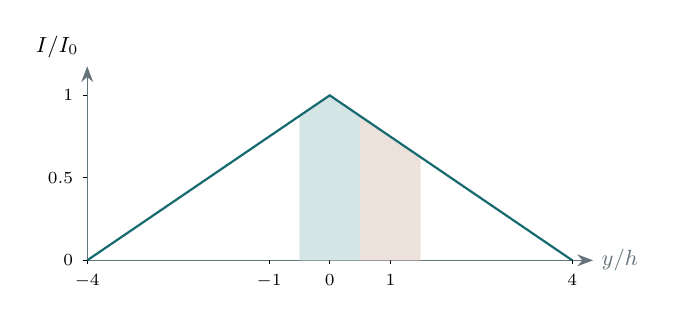
\begin{tikzpicture}[scale=.88,transform shape]
\draw[axis] (0,0.0)--(7.3,0.0) node[right] {$y/h$};
\draw[axis] (0,0)--(0,2.8);
\node[above left] at (0,2.8) {$I/I_0$};
\draw[thin] (0.000000,0.0)--(0.000000,-0.06);\node[below,font=\scriptsize] at (0.000000,-0.08) {$ -4 $};
\draw[thin] (2.625000,0.0)--(2.625000,-0.06);\node[below,font=\scriptsize] at (2.625000,-0.08) {$ -1 $};
\draw[thin] (3.500000,0.0)--(3.500000,-0.06);\node[below,font=\scriptsize] at (3.500000,-0.08) {$ 0 $};
\draw[thin] (4.375000,0.0)--(4.375000,-0.06);\node[below,font=\scriptsize] at (4.375000,-0.08) {$ 1 $};
\draw[thin] (7.000000,0.0)--(7.000000,-0.06);\node[below,font=\scriptsize] at (7.000000,-0.08) {$ 4 $};
\draw[thin] (0,0.000000)--(-.06,0.000000);\node[left,font=\scriptsize] at (-.08,0.000000) {$ 0 $};
\draw[thin] (0,1.190476)--(-.06,1.190476);\node[left,font=\scriptsize] at (-.08,1.190476) {$ 0.5 $};
\draw[thin] (0,2.380952)--(-.06,2.380952);\node[left,font=\scriptsize] at (-.08,2.380952) {$ 1 $};
\fill[accent!18] (3.0625000,0.0000000)--(3.0625000,2.0833333)--(3.5000000,2.3809524)--(3.9375000,2.0833333)--(3.9375000,0.0000000)--cycle;
\fill[warm!18] (3.9375000,0.0000000)--(3.9375000,2.0833333)--(4.8125000,1.4880952)--(4.8125000,0.0000000)--cycle;
\draw[thick,color=accent] plot coordinates {(0.0000000,0.0000000) (0.0291667,0.0198413) (0.0583333,0.0396825) (0.0875000,0.0595238) (0.1166667,0.0793651) (0.1458333,0.0992063) (0.1750000,0.1190476) (0.2041667,0.1388889) (0.2333333,0.1587302) (0.2625000,0.1785714) (0.2916667,0.1984127) (0.3208333,0.2182540) (0.3500000,0.2380952) (0.3791667,0.2579365) (0.4083333,0.2777778) (0.4375000,0.2976190) (0.4666667,0.3174603) (0.4958333,0.3373016) (0.5250000,0.3571429) (0.5541667,0.3769841) (0.5833333,0.3968254) (0.6125000,0.4166667) (0.6416667,0.4365079) (0.6708333,0.4563492) (0.7000000,0.4761905) (0.7291667,0.4960317) (0.7583333,0.5158730) (0.7875000,0.5357143) (0.8166667,0.5555556) (0.8458333,0.5753968) (0.8750000,0.5952381) (0.9041667,0.6150794) (0.9333333,0.6349206) (0.9625000,0.6547619) (0.9916667,0.6746032) (1.0208333,0.6944444) (1.0500000,0.7142857) (1.0791667,0.7341270) (1.1083333,0.7539683) (1.1375000,0.7738095) (1.1666667,0.7936508) (1.1958333,0.8134921) (1.2250000,0.8333333) (1.2541667,0.8531746) (1.2833333,0.8730159) (1.3125000,0.8928571) (1.3416667,0.9126984) (1.3708333,0.9325397) (1.4000000,0.9523810) (1.4291667,0.9722222) (1.4583333,0.9920635) (1.4875000,1.0119048) (1.5166667,1.0317460) (1.5458333,1.0515873) (1.5750000,1.0714286) (1.6041667,1.0912698) (1.6333333,1.1111111) (1.6625000,1.1309524) (1.6916667,1.1507937) (1.7208333,1.1706349) (1.7500000,1.1904762) (1.7791667,1.2103175) (1.8083333,1.2301587) (1.8375000,1.2500000) (1.8666667,1.2698413) (1.8958333,1.2896825) (1.9250000,1.3095238) (1.9541667,1.3293651) (1.9833333,1.3492063) (2.0125000,1.3690476) (2.0416667,1.3888889) (2.0708333,1.4087302) (2.1000000,1.4285714) (2.1291667,1.4484127) (2.1583333,1.4682540) (2.1875000,1.4880952) (2.2166667,1.5079365) (2.2458333,1.5277778) (2.2750000,1.5476190) (2.3041667,1.5674603) (2.3333333,1.5873016) (2.3625000,1.6071429) (2.3916667,1.6269841) (2.4208333,1.6468254) (2.4500000,1.6666667) (2.4791667,1.6865079) (2.5083333,1.7063492) (2.5375000,1.7261905) (2.5666667,1.7460317) (2.5958333,1.7658730) (2.6250000,1.7857143) (2.6541667,1.8055556) (2.6833333,1.8253968) (2.7125000,1.8452381) (2.7416667,1.8650794) (2.7708333,1.8849206) (2.8000000,1.9047619) (2.8291667,1.9246032) (2.8583333,1.9444444) (2.8875000,1.9642857) (2.9166667,1.9841270) (2.9458333,2.0039683) (2.9750000,2.0238095) (3.0041667,2.0436508) (3.0333333,2.0634921) (3.0625000,2.0833333) (3.0916667,2.1031746) (3.1208333,2.1230159) (3.1500000,2.1428571) (3.1791667,2.1626984) (3.2083333,2.1825397) (3.2375000,2.2023810) (3.2666667,2.2222222) (3.2958333,2.2420635) (3.3250000,2.2619048) (3.3541667,2.2817460) (3.3833333,2.3015873) (3.4125000,2.3214286) (3.4416667,2.3412698) (3.4708333,2.3611111) (3.5000000,2.3809524) (3.5291667,2.3611111) (3.5583333,2.3412698) (3.5875000,2.3214286) (3.6166667,2.3015873) (3.6458333,2.2817460) (3.6750000,2.2619048) (3.7041667,2.2420635) (3.7333333,2.2222222) (3.7625000,2.2023810) (3.7916667,2.1825397) (3.8208333,2.1626984) (3.8500000,2.1428571) (3.8791667,2.1230159) (3.9083333,2.1031746) (3.9375000,2.0833333) (3.9666667,2.0634921) (3.9958333,2.0436508) (4.0250000,2.0238095) (4.0541667,2.0039683) (4.0833333,1.9841270) (4.1125000,1.9642857) (4.1416667,1.9444444) (4.1708333,1.9246032) (4.2000000,1.9047619) (4.2291667,1.8849206) (4.2583333,1.8650794) (4.2875000,1.8452381) (4.3166667,1.8253968) (4.3458333,1.8055556) (4.3750000,1.7857143) (4.4041667,1.7658730) (4.4333333,1.7460317) (4.4625000,1.7261905) (4.4916667,1.7063492) (4.5208333,1.6865079) (4.5500000,1.6666667) (4.5791667,1.6468254) (4.6083333,1.6269841) (4.6375000,1.6071429) (4.6666667,1.5873016) (4.6958333,1.5674603) (4.7250000,1.5476190) (4.7541667,1.5277778) (4.7833333,1.5079365) (4.8125000,1.4880952) (4.8416667,1.4682540) (4.8708333,1.4484127) (4.9000000,1.4285714) (4.9291667,1.4087302) (4.9583333,1.3888889) (4.9875000,1.3690476) (5.0166667,1.3492063) (5.0458333,1.3293651) (5.0750000,1.3095238) (5.1041667,1.2896825) (5.1333333,1.2698413) (5.1625000,1.2500000) (5.1916667,1.2301587) (5.2208333,1.2103175) (5.2500000,1.1904762) (5.2791667,1.1706349) (5.3083333,1.1507937) (5.3375000,1.1309524) (5.3666667,1.1111111) (5.3958333,1.0912698) (5.4250000,1.0714286) (5.4541667,1.0515873) (5.4833333,1.0317460) (5.5125000,1.0119048) (5.5416667,0.9920635) (5.5708333,0.9722222) (5.6000000,0.9523810) (5.6291667,0.9325397) (5.6583333,0.9126984) (5.6875000,0.8928571) (5.7166667,0.8730159) (5.7458333,0.8531746) (5.7750000,0.8333333) (5.8041667,0.8134921) (5.8333333,0.7936508) (5.8625000,0.7738095) (5.8916667,0.7539683) (5.9208333,0.7341270) (5.9500000,0.7142857) (5.9791667,0.6944444) (6.0083333,0.6746032) (6.0375000,0.6547619) (6.0666667,0.6349206) (6.0958333,0.6150794) (6.1250000,0.5952381) (6.1541667,0.5753968) (6.1833333,0.5555556) (6.2125000,0.5357143) (6.2416667,0.5158730) (6.2708333,0.4960317) (6.3000000,0.4761905) (6.3291667,0.4563492) (6.3583333,0.4365079) (6.3875000,0.4166667) (6.4166667,0.3968254) (6.4458333,0.3769841) (6.4750000,0.3571429) (6.5041667,0.3373016) (6.5333333,0.3174603) (6.5625000,0.2976190) (6.5916667,0.2777778) (6.6208333,0.2579365) (6.6500000,0.2380952) (6.6791667,0.2182540) (6.7083333,0.1984127) (6.7375000,0.1785714) (6.7666667,0.1587302) (6.7958333,0.1388889) (6.8250000,0.1190476) (6.8541667,0.0992063) (6.8833333,0.0793651) (6.9125000,0.0595238) (6.9416667,0.0396825) (6.9708333,0.0198413) (7.0000000,0.0000000)};
\end{tikzpicture}
\figcaption{解图近1.2B\quad u等于1/2时，下条带负半到正半，上条带全在正半}
\end{minipage}\end{center}
令$u=y_0/h$，先计算正位移。$0\le u\le1$时，上条带全在正半轴，故
\[
 \frac{P_u}{hwI_0}=\int_u^{u+1}(1-v/4)\dd v
 =1-\frac{(u+1)^2-u^2}{8}=\frac78-\frac u4.
\]
下条带跨过光强尖点$v=0$，分别积分两侧线性函数：
\[
 \frac{P_l}{hwI_0}
 =\int_{u-1}^0(1+v/4)\dd v+\int_0^u(1-v/4)\dd v
 =\left(1-u-\frac{(1-u)^2}{8}\right)
  +\left(u-\frac{u^2}{8}\right).
\]
这两段也对应图中各自的平均照度：负半段长$h(1-u)$、中点为$-h(1-u)/2$，其平均光强为$I_0(7/8+u/8)$；正半段长$hu$、中点为$hu/2$，平均光强为$I_0(1-u/8)$。乘上各段投影面积后相加，即
\[
 P_l=hwI_0\left[(1-u)\left(\frac78+\frac u8\right)
 +u\left(1-\frac u8\right)\right].
\]
这正是上面积分中两个区间的面积，合并得到
\[
\frac{P_u}{hwI_0}=\frac78-\frac u4,\qquad
\frac{P_l}{hwI_0}=\frac78+\frac u4-\frac{u^2}4.
\]
这也可用两小段各自的中点光强乘长度，权重分别为$1-u$与$u$；整条跨零条带使用上面的两段平均。此时功率和为$hwI_0(7/4-u^2/4)$，功率差为$-hwI_0(u/2-u^2/4)$。

$1\le u\le3$时，两条带都在正半轴，每条带内光强均为线性函数，平均值等于各自中点值$I(y_0\pm h/2)$，因此
\[
\frac{P_u}{hwI_0}=\frac78-\frac u4,\quad
\frac{P_l}{hwI_0}=\frac98-\frac u4.
\]
功率和为$hwI_0(2-u/2)$，差为$-hwI_0/4$。两条相邻等宽带随棱镜一起平移，在线性光强段内，它们的平均值始终相差$I_0/4$，所以外段竖直力保持常量；两条带的总照度却随高度减小，水平力仍变化。关于$y=0$的光强对称使$P_u(-u)=P_l(u)$，所以水平方向力为偶函数、竖直方向力为奇函数。整个指定区间的结果为
\[
\boxed{\frac{cF_x}{hwI_0(1-\cos\theta)}
=\begin{cases}7/4-u^2/4,&|u|\leqslant1,\\2-|u|/2,&1\leqslant|u|\leqslant3,\end{cases}}
\]
\[
\boxed{\frac{cF_y}{hwI_0\sin\theta}
=\begin{cases}-\dfrac u2(1-\dfrac{|u|}2),&|u|\leqslant1,\\
-\dfrac{\operatorname{sgn}u}{4},&1\leqslant|u|\leqslant3.\end{cases}}
\]
解图近1.2C画两条分段函数。在$u=0$，水平系数为$7/4$、竖直力为零；在$|u|=1$，水平系数为$3/2$，竖直系数为$\mp1/4$，两段连续衔接；在$|u|=3$，水平系数仍为$1/2$。外段水平力随$|u|$线性下降，竖直力为回复方向的常量。它们由条带积分的区间变化给出。
\begin{center}\begin{minipage}{.98\linewidth}\centering
\begin{tikzpicture}[scale=.88,transform shape]
\draw[axis] (0,0.3488372093023256)--(7.3,0.3488372093023256) node[right] {$u=y_0/h$};
\draw[axis] (0,0)--(0,2.8);
\node[above left] at (0,2.8) {归一化光力};
\draw[thin] (0.000000,0.3488372093023256)--(0.000000,0.2888372093023256);\node[below,font=\scriptsize] at (0.000000,0.2688372093023256) {$ -3 $};
\draw[thin] (2.333333,0.3488372093023256)--(2.333333,0.2888372093023256);\node[below,font=\scriptsize] at (2.333333,0.2688372093023256) {$ -1 $};
\draw[thin] (3.500000,0.3488372093023256)--(3.500000,0.2888372093023256);\node[below,font=\scriptsize] at (3.500000,0.2688372093023256) {$ 0 $};
\draw[thin] (4.666667,0.3488372093023256)--(4.666667,0.2888372093023256);\node[below,font=\scriptsize] at (4.666667,0.2688372093023256) {$ 1 $};
\draw[thin] (7.000000,0.3488372093023256)--(7.000000,0.2888372093023256);\node[below,font=\scriptsize] at (7.000000,0.2688372093023256) {$ 3 $};
\draw[thin] (0,0.058140)--(-.06,0.058140);\node[left,font=\scriptsize] at (-.08,0.058140) {$ -0.25 $};
\draw[thin] (0,0.348837)--(-.06,0.348837);\node[left,font=\scriptsize] at (-.08,0.348837) {$ 0 $};
\draw[thin] (0,0.930233)--(-.06,0.930233);\node[left,font=\scriptsize] at (-.08,0.930233) {$ 0.5 $};
\draw[thin] (0,2.093023)--(-.06,2.093023);\node[left,font=\scriptsize] at (-.08,2.093023) {$ 1.5 $};
\draw[thin] (0,2.383721)--(-.06,2.383721);\node[left,font=\scriptsize] at (-.08,2.383721) {$ 1.75 $};
\draw[thick,color=accent] plot coordinates {(0.0000000,0.9302326) (0.0291667,0.9447674) (0.0583333,0.9593023) (0.0875000,0.9738372) (0.1166667,0.9883721) (0.1458333,1.0029070) (0.1750000,1.0174419) (0.2041667,1.0319767) (0.2333333,1.0465116) (0.2625000,1.0610465) (0.2916667,1.0755814) (0.3208333,1.0901163) (0.3500000,1.1046512) (0.3791667,1.1191860) (0.4083333,1.1337209) (0.4375000,1.1482558) (0.4666667,1.1627907) (0.4958333,1.1773256) (0.5250000,1.1918605) (0.5541667,1.2063953) (0.5833333,1.2209302) (0.6125000,1.2354651) (0.6416667,1.2500000) (0.6708333,1.2645349) (0.7000000,1.2790698) (0.7291667,1.2936047) (0.7583333,1.3081395) (0.7875000,1.3226744) (0.8166667,1.3372093) (0.8458333,1.3517442) (0.8750000,1.3662791) (0.9041667,1.3808140) (0.9333333,1.3953488) (0.9625000,1.4098837) (0.9916667,1.4244186) (1.0208333,1.4389535) (1.0500000,1.4534884) (1.0791667,1.4680233) (1.1083333,1.4825581) (1.1375000,1.4970930) (1.1666667,1.5116279) (1.1958333,1.5261628) (1.2250000,1.5406977) (1.2541667,1.5552326) (1.2833333,1.5697674) (1.3125000,1.5843023) (1.3416667,1.5988372) (1.3708333,1.6133721) (1.4000000,1.6279070) (1.4291667,1.6424419) (1.4583333,1.6569767) (1.4875000,1.6715116) (1.5166667,1.6860465) (1.5458333,1.7005814) (1.5750000,1.7151163) (1.6041667,1.7296512) (1.6333333,1.7441860) (1.6625000,1.7587209) (1.6916667,1.7732558) (1.7208333,1.7877907) (1.7500000,1.8023256) (1.7791667,1.8168605) (1.8083333,1.8313953) (1.8375000,1.8459302) (1.8666667,1.8604651) (1.8958333,1.8750000) (1.9250000,1.8895349) (1.9541667,1.9040698) (1.9833333,1.9186047) (2.0125000,1.9331395) (2.0416667,1.9476744) (2.0708333,1.9622093) (2.1000000,1.9767442) (2.1291667,1.9912791) (2.1583333,2.0058140) (2.1875000,2.0203488) (2.2166667,2.0348837) (2.2458333,2.0494186) (2.2750000,2.0639535) (2.3041667,2.0784884) (2.3333333,2.0930233) (2.3625000,2.1073765) (2.3916667,2.1213663) (2.4208333,2.1349927) (2.4500000,2.1482558) (2.4791667,2.1611555) (2.5083333,2.1736919) (2.5375000,2.1858648) (2.5666667,2.1976744) (2.5958333,2.2091206) (2.6250000,2.2202035) (2.6541667,2.2309230) (2.6833333,2.2412791) (2.7125000,2.2512718) (2.7416667,2.2609012) (2.7708333,2.2701672) (2.8000000,2.2790698) (2.8291667,2.2876090) (2.8583333,2.2957849) (2.8875000,2.3035974) (2.9166667,2.3110465) (2.9458333,2.3181323) (2.9750000,2.3248547) (3.0041667,2.3312137) (3.0333333,2.3372093) (3.0625000,2.3428416) (3.0916667,2.3481105) (3.1208333,2.3530160) (3.1500000,2.3575581) (3.1791667,2.3617369) (3.2083333,2.3655523) (3.2375000,2.3690044) (3.2666667,2.3720930) (3.2958333,2.3748183) (3.3250000,2.3771802) (3.3541667,2.3791788) (3.3833333,2.3808140) (3.4125000,2.3820858) (3.4416667,2.3829942) (3.4708333,2.3835392) (3.5000000,2.3837209) (3.5291667,2.3835392) (3.5583333,2.3829942) (3.5875000,2.3820858) (3.6166667,2.3808140) (3.6458333,2.3791788) (3.6750000,2.3771802) (3.7041667,2.3748183) (3.7333333,2.3720930) (3.7625000,2.3690044) (3.7916667,2.3655523) (3.8208333,2.3617369) (3.8500000,2.3575581) (3.8791667,2.3530160) (3.9083333,2.3481105) (3.9375000,2.3428416) (3.9666667,2.3372093) (3.9958333,2.3312137) (4.0250000,2.3248547) (4.0541667,2.3181323) (4.0833333,2.3110465) (4.1125000,2.3035974) (4.1416667,2.2957849) (4.1708333,2.2876090) (4.2000000,2.2790698) (4.2291667,2.2701672) (4.2583333,2.2609012) (4.2875000,2.2512718) (4.3166667,2.2412791) (4.3458333,2.2309230) (4.3750000,2.2202035) (4.4041667,2.2091206) (4.4333333,2.1976744) (4.4625000,2.1858648) (4.4916667,2.1736919) (4.5208333,2.1611555) (4.5500000,2.1482558) (4.5791667,2.1349927) (4.6083333,2.1213663) (4.6375000,2.1073765) (4.6666667,2.0930233) (4.6958333,2.0784884) (4.7250000,2.0639535) (4.7541667,2.0494186) (4.7833333,2.0348837) (4.8125000,2.0203488) (4.8416667,2.0058140) (4.8708333,1.9912791) (4.9000000,1.9767442) (4.9291667,1.9622093) (4.9583333,1.9476744) (4.9875000,1.9331395) (5.0166667,1.9186047) (5.0458333,1.9040698) (5.0750000,1.8895349) (5.1041667,1.8750000) (5.1333333,1.8604651) (5.1625000,1.8459302) (5.1916667,1.8313953) (5.2208333,1.8168605) (5.2500000,1.8023256) (5.2791667,1.7877907) (5.3083333,1.7732558) (5.3375000,1.7587209) (5.3666667,1.7441860) (5.3958333,1.7296512) (5.4250000,1.7151163) (5.4541667,1.7005814) (5.4833333,1.6860465) (5.5125000,1.6715116) (5.5416667,1.6569767) (5.5708333,1.6424419) (5.6000000,1.6279070) (5.6291667,1.6133721) (5.6583333,1.5988372) (5.6875000,1.5843023) (5.7166667,1.5697674) (5.7458333,1.5552326) (5.7750000,1.5406977) (5.8041667,1.5261628) (5.8333333,1.5116279) (5.8625000,1.4970930) (5.8916667,1.4825581) (5.9208333,1.4680233) (5.9500000,1.4534884) (5.9791667,1.4389535) (6.0083333,1.4244186) (6.0375000,1.4098837) (6.0666667,1.3953488) (6.0958333,1.3808140) (6.1250000,1.3662791) (6.1541667,1.3517442) (6.1833333,1.3372093) (6.2125000,1.3226744) (6.2416667,1.3081395) (6.2708333,1.2936047) (6.3000000,1.2790698) (6.3291667,1.2645349) (6.3583333,1.2500000) (6.3875000,1.2354651) (6.4166667,1.2209302) (6.4458333,1.2063953) (6.4750000,1.1918605) (6.5041667,1.1773256) (6.5333333,1.1627907) (6.5625000,1.1482558) (6.5916667,1.1337209) (6.6208333,1.1191860) (6.6500000,1.1046512) (6.6791667,1.0901163) (6.7083333,1.0755814) (6.7375000,1.0610465) (6.7666667,1.0465116) (6.7958333,1.0319767) (6.8250000,1.0174419) (6.8541667,1.0029070) (6.8833333,0.9883721) (6.9125000,0.9738372) (6.9416667,0.9593023) (6.9708333,0.9447674) (7.0000000,0.9302326)};
\draw[thick,color=accent] (7.65,2.55)--(8.15,2.55);\node[right,font=\scriptsize] at (8.2,2.55) {$cF_x/[hwI_0(1-\cos\theta)]$};
\draw[thick,dashed,color=warm] plot coordinates {(0.0000000,0.6395349) (0.0291667,0.6395349) (0.0583333,0.6395349) (0.0875000,0.6395349) (0.1166667,0.6395349) (0.1458333,0.6395349) (0.1750000,0.6395349) (0.2041667,0.6395349) (0.2333333,0.6395349) (0.2625000,0.6395349) (0.2916667,0.6395349) (0.3208333,0.6395349) (0.3500000,0.6395349) (0.3791667,0.6395349) (0.4083333,0.6395349) (0.4375000,0.6395349) (0.4666667,0.6395349) (0.4958333,0.6395349) (0.5250000,0.6395349) (0.5541667,0.6395349) (0.5833333,0.6395349) (0.6125000,0.6395349) (0.6416667,0.6395349) (0.6708333,0.6395349) (0.7000000,0.6395349) (0.7291667,0.6395349) (0.7583333,0.6395349) (0.7875000,0.6395349) (0.8166667,0.6395349) (0.8458333,0.6395349) (0.8750000,0.6395349) (0.9041667,0.6395349) (0.9333333,0.6395349) (0.9625000,0.6395349) (0.9916667,0.6395349) (1.0208333,0.6395349) (1.0500000,0.6395349) (1.0791667,0.6395349) (1.1083333,0.6395349) (1.1375000,0.6395349) (1.1666667,0.6395349) (1.1958333,0.6395349) (1.2250000,0.6395349) (1.2541667,0.6395349) (1.2833333,0.6395349) (1.3125000,0.6395349) (1.3416667,0.6395349) (1.3708333,0.6395349) (1.4000000,0.6395349) (1.4291667,0.6395349) (1.4583333,0.6395349) (1.4875000,0.6395349) (1.5166667,0.6395349) (1.5458333,0.6395349) (1.5750000,0.6395349) (1.6041667,0.6395349) (1.6333333,0.6395349) (1.6625000,0.6395349) (1.6916667,0.6395349) (1.7208333,0.6395349) (1.7500000,0.6395349) (1.7791667,0.6395349) (1.8083333,0.6395349) (1.8375000,0.6395349) (1.8666667,0.6395349) (1.8958333,0.6395349) (1.9250000,0.6395349) (1.9541667,0.6395349) (1.9833333,0.6395349) (2.0125000,0.6395349) (2.0416667,0.6395349) (2.0708333,0.6395349) (2.1000000,0.6395349) (2.1291667,0.6395349) (2.1583333,0.6395349) (2.1875000,0.6395349) (2.2166667,0.6395349) (2.2458333,0.6395349) (2.2750000,0.6395349) (2.3041667,0.6395349) (2.3333333,0.6395349) (2.3625000,0.6393532) (2.3916667,0.6388081) (2.4208333,0.6378997) (2.4500000,0.6366279) (2.4791667,0.6349927) (2.5083333,0.6329942) (2.5375000,0.6306323) (2.5666667,0.6279070) (2.5958333,0.6248183) (2.6250000,0.6213663) (2.6541667,0.6175509) (2.6833333,0.6133721) (2.7125000,0.6088299) (2.7416667,0.6039244) (2.7708333,0.5986555) (2.8000000,0.5930233) (2.8291667,0.5870276) (2.8583333,0.5806686) (2.8875000,0.5739462) (2.9166667,0.5668605) (2.9458333,0.5594113) (2.9750000,0.5515988) (3.0041667,0.5434230) (3.0333333,0.5348837) (3.0625000,0.5259811) (3.0916667,0.5167151) (3.1208333,0.5070858) (3.1500000,0.4970930) (3.1791667,0.4867369) (3.2083333,0.4760174) (3.2375000,0.4649346) (3.2666667,0.4534884) (3.2958333,0.4416788) (3.3250000,0.4295058) (3.3541667,0.4169695) (3.3833333,0.4040698) (3.4125000,0.3908067) (3.4416667,0.3771802) (3.4708333,0.3631904) (3.5000000,0.3488372) (3.5291667,0.3344840) (3.5583333,0.3204942) (3.5875000,0.3068677) (3.6166667,0.2936047) (3.6458333,0.2807049) (3.6750000,0.2681686) (3.7041667,0.2559956) (3.7333333,0.2441860) (3.7625000,0.2327398) (3.7916667,0.2216570) (3.8208333,0.2109375) (3.8500000,0.2005814) (3.8791667,0.1905887) (3.9083333,0.1809593) (3.9375000,0.1716933) (3.9666667,0.1627907) (3.9958333,0.1542515) (4.0250000,0.1460756) (4.0541667,0.1382631) (4.0833333,0.1308140) (4.1125000,0.1237282) (4.1416667,0.1170058) (4.1708333,0.1106468) (4.2000000,0.1046512) (4.2291667,0.0990189) (4.2583333,0.0937500) (4.2875000,0.0888445) (4.3166667,0.0843023) (4.3458333,0.0801235) (4.3750000,0.0763081) (4.4041667,0.0728561) (4.4333333,0.0697674) (4.4625000,0.0670422) (4.4916667,0.0646802) (4.5208333,0.0626817) (4.5500000,0.0610465) (4.5791667,0.0597747) (4.6083333,0.0588663) (4.6375000,0.0583212) (4.6666667,0.0581395) (4.6958333,0.0581395) (4.7250000,0.0581395) (4.7541667,0.0581395) (4.7833333,0.0581395) (4.8125000,0.0581395) (4.8416667,0.0581395) (4.8708333,0.0581395) (4.9000000,0.0581395) (4.9291667,0.0581395) (4.9583333,0.0581395) (4.9875000,0.0581395) (5.0166667,0.0581395) (5.0458333,0.0581395) (5.0750000,0.0581395) (5.1041667,0.0581395) (5.1333333,0.0581395) (5.1625000,0.0581395) (5.1916667,0.0581395) (5.2208333,0.0581395) (5.2500000,0.0581395) (5.2791667,0.0581395) (5.3083333,0.0581395) (5.3375000,0.0581395) (5.3666667,0.0581395) (5.3958333,0.0581395) (5.4250000,0.0581395) (5.4541667,0.0581395) (5.4833333,0.0581395) (5.5125000,0.0581395) (5.5416667,0.0581395) (5.5708333,0.0581395) (5.6000000,0.0581395) (5.6291667,0.0581395) (5.6583333,0.0581395) (5.6875000,0.0581395) (5.7166667,0.0581395) (5.7458333,0.0581395) (5.7750000,0.0581395) (5.8041667,0.0581395) (5.8333333,0.0581395) (5.8625000,0.0581395) (5.8916667,0.0581395) (5.9208333,0.0581395) (5.9500000,0.0581395) (5.9791667,0.0581395) (6.0083333,0.0581395) (6.0375000,0.0581395) (6.0666667,0.0581395) (6.0958333,0.0581395) (6.1250000,0.0581395) (6.1541667,0.0581395) (6.1833333,0.0581395) (6.2125000,0.0581395) (6.2416667,0.0581395) (6.2708333,0.0581395) (6.3000000,0.0581395) (6.3291667,0.0581395) (6.3583333,0.0581395) (6.3875000,0.0581395) (6.4166667,0.0581395) (6.4458333,0.0581395) (6.4750000,0.0581395) (6.5041667,0.0581395) (6.5333333,0.0581395) (6.5625000,0.0581395) (6.5916667,0.0581395) (6.6208333,0.0581395) (6.6500000,0.0581395) (6.6791667,0.0581395) (6.7083333,0.0581395) (6.7375000,0.0581395) (6.7666667,0.0581395) (6.7958333,0.0581395) (6.8250000,0.0581395) (6.8541667,0.0581395) (6.8833333,0.0581395) (6.9125000,0.0581395) (6.9416667,0.0581395) (6.9708333,0.0581395) (7.0000000,0.0581395)};
\draw[thick,dashed,color=warm] (7.65,2.0999999999999996)--(8.15,2.0999999999999996);\node[right,font=\scriptsize] at (8.2,2.0999999999999996) {$cF_y/(hwI_0\sin\theta)$};
\end{tikzpicture}
\figcaption{解图近1.2C\quad 完整分段光力在中央与外段连续衔接}
\end{minipage}\end{center}
（3）代$\alpha=30^\circ,n=1.5$，先得$\beta=19.4712^\circ$，内部光线对底面法线的夹角为$10.5288^\circ$，第二次折射得到$\theta=15.9080^\circ$。三角形横截面的底边为$2h$，沿$x$的高为$h\tan\alpha$，所以截面积为$h^2\tan\alpha$，乘厚度$w$后得到
\[
V=h^2w\tan\alpha,\quad m=\rho h^2w\tan\alpha=1.4434\times10^{-10}\,\mathrm{kg},
\quad \theta=15.9080^\circ.
\]
这里$h=10^{-5}\,\mathrm m,w=10^{-3}\,\mathrm m,\rho=2.5\times10^3\,\mathrm{kg/m^3}$，质量为$1.4434\times10^{-10}\,\mathrm{kg}$，取$g=9.8\,\mathrm{m/s^2}$时重力约$1.4145\times10^{-9}\,\mathrm N$。在$u=-1/2$处，竖直分段系数为$1/4-1/16=3/16$，因而$F_y=3hwI_0\sin\theta/(16c)$。令它与重力相等，
\[
I_0=\frac{16cmg}{3hw\sin\theta}\simeq8.26\times10^8\,\mathrm{W/m^2}.
\]
接下来求整束光功率。其宽度为$8h$，光强剖面的三角形面积为$\tfrac12(8h)I_0=4hI_0$，再乘沿$z$的宽度$w$，所以
\[
\boxed{P=w\int_{-4h}^{4h}I(y)\dd y=4hwI_0\simeq33.0\,\mathrm W}.
\]
棱镜仅截获其中一部分光，激光器总功率使用整个$-4h$到$4h$范围。上述等式给竖直平衡，水平方向的$F_x$仍为正。在该偏移处，水平分段系数为$7/4-(1/2)^2/4=27/16$，因此
\[
 \frac{F_x}{mg}=\frac{27(1-\cos\theta)}{3\sin\theta}
 =9\tan\frac{\theta}{2}.
\]
这项前进力与已平衡的竖直分量具有相同光功率尺度。要求棱镜整体静止时，另以水平约束或对向光束配平；若只释放竖直自由度，便在对应偏移处讨论竖直平衡。

（4）本问去掉重力，并取$I_0=10^8\,\mathrm{W/m^2}$，区别于上一问重力平衡所需的峰值。中心段的完整竖直力为
\[
 F_y=-\frac{wI_0\sin\theta}{2c}\,y
 \left(1-\frac{|y|}{2h}\right),\qquad |y|\le h.
\]
在$y=0$附近，线性项为$-Ky$，从质量和该系数得到
\[
K=\frac{wI_0\sin\theta}{2c},\quad
m\ddot y+Ky\simeq0,\quad
\boxed{T_0=2\pi\sqrt{\frac mK}
=2\pi\sqrt{\frac{2c\rho h^2\tan\alpha}{I_0\sin\theta}}
\simeq1.117\times10^{-2}\,\mathrm s}.
\]
解图近1.2D把实际回复势与线性抛物线放在一起。指定振幅$a=h/20$，全程$|y|/(2h)\le0.025$，故上式的非线性项是小修正，$T_0$为小振动周期。振动方向的能量由$\dd U/\dd y=-F_y$给出：对正$y$积分并按偶对称延伸，
\[
U(y)=\frac K2y^2-\frac{K}{6h}|y|^3,\qquad
T(a)=4\sqrt{\frac m2}\int_0^a\frac{\dd y}{\sqrt{U(a)-U(y)}}.
\]
其中$U(0)=0$，总竖直能量为$U(a)$，$m\dot y^2/2=U(a)-U(y)$。从中心积分到转折点的时间为一个周期的四分之一，因而得到上面的有限振幅周期式。解图近1.2D中$|y|^3$项使势能曲线低于抛物线，振幅增加时周期略长。令$y=a\sin\psi$，将转折点处的平方根因子提出，得
\[
 \frac{T(a)}{T_0}=\frac2\pi\int_0^{\pi/2}
 \left[1-\frac{a}{3h}\frac{1-\sin^3\psi}{1-\sin^2\psi}\right]^{-1/2}\dd\psi.
\]
括号内的比值写成$\sin\psi+1/(1+\sin\psi)$，在$\psi=\pi/2$处按连续值取$3/2$。利用
\[
 \int_0^{\pi/2}\sin\psi\,\dd\psi=1,\qquad
 \int_0^{\pi/2}\frac{\dd\psi}{1+\sin\psi}
 =\left[-\frac{\cos\psi}{1+\sin\psi}\right]_0^{\pi/2}=1,
\]
将被积式按$a/h$展开到一阶，便有
\[
 \frac{T(a)}{T_0}=1+\frac{2a}{3\pi h}
 +O\!\left(\frac{a^2}{h^2}\right).
\]
因此$a=h/20$时，首阶周期增加约$1.061\%$；完整能量积分给$T(a)/T_0\simeq1.01079$。线性周期与有限振幅周期都由同一条回复势得到，图中的软化项决定这项差别。
\begin{center}\begin{minipage}{.98\linewidth}\centering
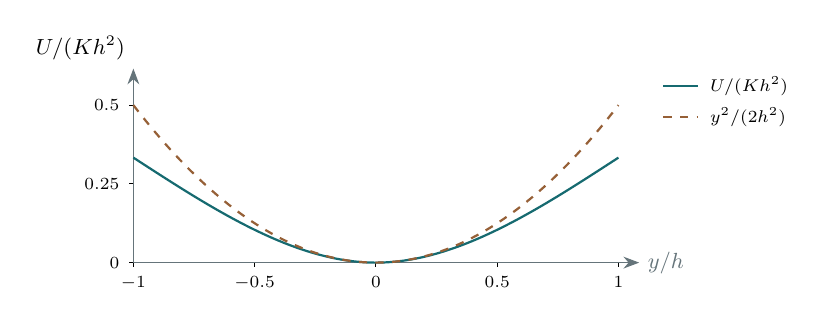
\begin{tikzpicture}[scale=.88,transform shape]
\draw[axis] (0,0.0)--(7.3,0.0) node[right] {$y/h$};
\draw[axis] (0,0)--(0,2.8);
\node[above left] at (0,2.8) {$U/(Kh^2)$};
\draw[thin] (0.000000,0.0)--(0.000000,-0.06);\node[below,font=\scriptsize] at (0.000000,-0.08) {$ -1 $};
\draw[thin] (1.750000,0.0)--(1.750000,-0.06);\node[below,font=\scriptsize] at (1.750000,-0.08) {$ -0.5 $};
\draw[thin] (3.500000,0.0)--(3.500000,-0.06);\node[below,font=\scriptsize] at (3.500000,-0.08) {$ 0 $};
\draw[thin] (5.250000,0.0)--(5.250000,-0.06);\node[below,font=\scriptsize] at (5.250000,-0.08) {$ 0.5 $};
\draw[thin] (7.000000,0.0)--(7.000000,-0.06);\node[below,font=\scriptsize] at (7.000000,-0.08) {$ 1 $};
\draw[thin] (0,0.000000)--(-.06,0.000000);\node[left,font=\scriptsize] at (-.08,0.000000) {$ 0 $};
\draw[thin] (0,1.136364)--(-.06,1.136364);\node[left,font=\scriptsize] at (-.08,1.136364) {$ 0.25 $};
\draw[thin] (0,2.272727)--(-.06,2.272727);\node[left,font=\scriptsize] at (-.08,2.272727) {$ 0.5 $};
\draw[thick,color=accent] plot coordinates {(0.0000000,1.5151515) (0.0291667,1.4962126) (0.0583333,1.4772762) (0.0875000,1.4583452) (0.1166667,1.4394220) (0.1458333,1.4205093) (0.1750000,1.4016098) (0.2041667,1.3827261) (0.2333333,1.3638608) (0.2625000,1.3450166) (0.2916667,1.3261960) (0.3208333,1.3074017) (0.3500000,1.2886364) (0.3791667,1.2699026) (0.4083333,1.2512030) (0.4375000,1.2325402) (0.4666667,1.2139169) (0.4958333,1.1953357) (0.5250000,1.1767992) (0.5541667,1.1583101) (0.5833333,1.1398709) (0.6125000,1.1214844) (0.6416667,1.1031531) (0.6708333,1.0848796) (0.7000000,1.0666667) (0.7291667,1.0485169) (0.7583333,1.0304328) (0.7875000,1.0124171) (0.8166667,0.9944725) (0.8458333,0.9766015) (0.8750000,0.9588068) (0.9041667,0.9410910) (0.9333333,0.9234568) (0.9625000,0.9059067) (0.9916667,0.8884435) (1.0208333,0.8710696) (1.0500000,0.8537879) (1.0791667,0.8366008) (1.1083333,0.8195111) (1.1375000,0.8025213) (1.1666667,0.7856341) (1.1958333,0.7688521) (1.2250000,0.7521780) (1.2541667,0.7356144) (1.2833333,0.7191639) (1.3125000,0.7028291) (1.3416667,0.6866127) (1.3708333,0.6705172) (1.4000000,0.6545455) (1.4291667,0.6386999) (1.4583333,0.6229833) (1.4875000,0.6073982) (1.5166667,0.5919473) (1.5458333,0.5766331) (1.5750000,0.5614583) (1.6041667,0.5464256) (1.6333333,0.5315376) (1.6625000,0.5167969) (1.6916667,0.5022061) (1.7208333,0.4877679) (1.7500000,0.4734848) (1.7791667,0.4593597) (1.8083333,0.4453949) (1.8375000,0.4315933) (1.8666667,0.4179574) (1.8958333,0.4044898) (1.9250000,0.3911932) (1.9541667,0.3780702) (1.9833333,0.3651235) (2.0125000,0.3523556) (2.0416667,0.3397692) (2.0708333,0.3273670) (2.1000000,0.3151515) (2.1291667,0.3031254) (2.1583333,0.2912914) (2.1875000,0.2796520) (2.2166667,0.2682099) (2.2458333,0.2569677) (2.2750000,0.2459280) (2.3041667,0.2350936) (2.3333333,0.2244669) (2.3625000,0.2140507) (2.3916667,0.2038475) (2.4208333,0.1938600) (2.4500000,0.1840909) (2.4791667,0.1745427) (2.5083333,0.1652182) (2.5375000,0.1561198) (2.5666667,0.1472503) (2.5958333,0.1386123) (2.6250000,0.1302083) (2.6541667,0.1220412) (2.6833333,0.1141134) (2.7125000,0.1064276) (2.7416667,0.0989864) (2.7708333,0.0917925) (2.8000000,0.0848485) (2.8291667,0.0781570) (2.8583333,0.0717207) (2.8875000,0.0655421) (2.9166667,0.0596240) (2.9458333,0.0539689) (2.9750000,0.0485795) (3.0041667,0.0434585) (3.0333333,0.0386083) (3.0625000,0.0340317) (3.0916667,0.0297313) (3.1208333,0.0257098) (3.1500000,0.0219697) (3.1791667,0.0185137) (3.2083333,0.0153444) (3.2375000,0.0124645) (3.2666667,0.0098765) (3.2958333,0.0075832) (3.3250000,0.0055871) (3.3541667,0.0038909) (3.3833333,0.0024972) (3.4125000,0.0014086) (3.4416667,0.0006278) (3.4708333,0.0001574) (3.5000000,0.0000000) (3.5291667,0.0001574) (3.5583333,0.0006278) (3.5875000,0.0014086) (3.6166667,0.0024972) (3.6458333,0.0038909) (3.6750000,0.0055871) (3.7041667,0.0075832) (3.7333333,0.0098765) (3.7625000,0.0124645) (3.7916667,0.0153444) (3.8208333,0.0185137) (3.8500000,0.0219697) (3.8791667,0.0257098) (3.9083333,0.0297313) (3.9375000,0.0340317) (3.9666667,0.0386083) (3.9958333,0.0434585) (4.0250000,0.0485795) (4.0541667,0.0539689) (4.0833333,0.0596240) (4.1125000,0.0655421) (4.1416667,0.0717207) (4.1708333,0.0781570) (4.2000000,0.0848485) (4.2291667,0.0917925) (4.2583333,0.0989864) (4.2875000,0.1064276) (4.3166667,0.1141134) (4.3458333,0.1220412) (4.3750000,0.1302083) (4.4041667,0.1386123) (4.4333333,0.1472503) (4.4625000,0.1561198) (4.4916667,0.1652182) (4.5208333,0.1745427) (4.5500000,0.1840909) (4.5791667,0.1938600) (4.6083333,0.2038475) (4.6375000,0.2140507) (4.6666667,0.2244669) (4.6958333,0.2350936) (4.7250000,0.2459280) (4.7541667,0.2569677) (4.7833333,0.2682099) (4.8125000,0.2796520) (4.8416667,0.2912914) (4.8708333,0.3031254) (4.9000000,0.3151515) (4.9291667,0.3273670) (4.9583333,0.3397692) (4.9875000,0.3523556) (5.0166667,0.3651235) (5.0458333,0.3780702) (5.0750000,0.3911932) (5.1041667,0.4044898) (5.1333333,0.4179574) (5.1625000,0.4315933) (5.1916667,0.4453949) (5.2208333,0.4593597) (5.2500000,0.4734848) (5.2791667,0.4877679) (5.3083333,0.5022061) (5.3375000,0.5167969) (5.3666667,0.5315376) (5.3958333,0.5464256) (5.4250000,0.5614583) (5.4541667,0.5766331) (5.4833333,0.5919473) (5.5125000,0.6073982) (5.5416667,0.6229833) (5.5708333,0.6386999) (5.6000000,0.6545455) (5.6291667,0.6705172) (5.6583333,0.6866127) (5.6875000,0.7028291) (5.7166667,0.7191639) (5.7458333,0.7356144) (5.7750000,0.7521780) (5.8041667,0.7688521) (5.8333333,0.7856341) (5.8625000,0.8025213) (5.8916667,0.8195111) (5.9208333,0.8366008) (5.9500000,0.8537879) (5.9791667,0.8710696) (6.0083333,0.8884435) (6.0375000,0.9059067) (6.0666667,0.9234568) (6.0958333,0.9410910) (6.1250000,0.9588068) (6.1541667,0.9766015) (6.1833333,0.9944725) (6.2125000,1.0124171) (6.2416667,1.0304328) (6.2708333,1.0485169) (6.3000000,1.0666667) (6.3291667,1.0848796) (6.3583333,1.1031531) (6.3875000,1.1214844) (6.4166667,1.1398709) (6.4458333,1.1583101) (6.4750000,1.1767992) (6.5041667,1.1953357) (6.5333333,1.2139169) (6.5625000,1.2325402) (6.5916667,1.2512030) (6.6208333,1.2699026) (6.6500000,1.2886364) (6.6791667,1.3074017) (6.7083333,1.3261960) (6.7375000,1.3450166) (6.7666667,1.3638608) (6.7958333,1.3827261) (6.8250000,1.4016098) (6.8541667,1.4205093) (6.8833333,1.4394220) (6.9125000,1.4583452) (6.9416667,1.4772762) (6.9708333,1.4962126) (7.0000000,1.5151515)};
\draw[thick,color=accent] (7.65,2.55)--(8.15,2.55);\node[right,font=\scriptsize] at (8.2,2.55) {$U/(Kh^2)$};
\draw[thick,dashed,color=warm] plot coordinates {(0.0000000,2.2727273) (0.0291667,2.2350063) (0.0583333,2.1976010) (0.0875000,2.1605114) (0.1166667,2.1237374) (0.1458333,2.0872790) (0.1750000,2.0511364) (0.2041667,2.0153093) (0.2333333,1.9797980) (0.2625000,1.9446023) (0.2916667,1.9097222) (0.3208333,1.8751578) (0.3500000,1.8409091) (0.3791667,1.8069760) (0.4083333,1.7733586) (0.4375000,1.7400568) (0.4666667,1.7070707) (0.4958333,1.6744003) (0.5250000,1.6420455) (0.5541667,1.6100063) (0.5833333,1.5782828) (0.6125000,1.5468750) (0.6416667,1.5157828) (0.6708333,1.4850063) (0.7000000,1.4545455) (0.7291667,1.4244003) (0.7583333,1.3945707) (0.7875000,1.3650568) (0.8166667,1.3358586) (0.8458333,1.3069760) (0.8750000,1.2784091) (0.9041667,1.2501578) (0.9333333,1.2222222) (0.9625000,1.1946023) (0.9916667,1.1672980) (1.0208333,1.1403093) (1.0500000,1.1136364) (1.0791667,1.0872790) (1.1083333,1.0612374) (1.1375000,1.0355114) (1.1666667,1.0101010) (1.1958333,0.9850063) (1.2250000,0.9602273) (1.2541667,0.9357639) (1.2833333,0.9116162) (1.3125000,0.8877841) (1.3416667,0.8642677) (1.3708333,0.8410669) (1.4000000,0.8181818) (1.4291667,0.7956124) (1.4583333,0.7733586) (1.4875000,0.7514205) (1.5166667,0.7297980) (1.5458333,0.7084912) (1.5750000,0.6875000) (1.6041667,0.6668245) (1.6333333,0.6464646) (1.6625000,0.6264205) (1.6916667,0.6066919) (1.7208333,0.5872790) (1.7500000,0.5681818) (1.7791667,0.5494003) (1.8083333,0.5309343) (1.8375000,0.5127841) (1.8666667,0.4949495) (1.8958333,0.4774306) (1.9250000,0.4602273) (1.9541667,0.4433396) (1.9833333,0.4267677) (2.0125000,0.4105114) (2.0416667,0.3945707) (2.0708333,0.3789457) (2.1000000,0.3636364) (2.1291667,0.3486427) (2.1583333,0.3339646) (2.1875000,0.3196023) (2.2166667,0.3055556) (2.2458333,0.2918245) (2.2750000,0.2784091) (2.3041667,0.2653093) (2.3333333,0.2525253) (2.3625000,0.2400568) (2.3916667,0.2279040) (2.4208333,0.2160669) (2.4500000,0.2045455) (2.4791667,0.1933396) (2.5083333,0.1824495) (2.5375000,0.1718750) (2.5666667,0.1616162) (2.5958333,0.1516730) (2.6250000,0.1420455) (2.6541667,0.1327336) (2.6833333,0.1237374) (2.7125000,0.1150568) (2.7416667,0.1066919) (2.7708333,0.0986427) (2.8000000,0.0909091) (2.8291667,0.0834912) (2.8583333,0.0763889) (2.8875000,0.0696023) (2.9166667,0.0631313) (2.9458333,0.0569760) (2.9750000,0.0511364) (3.0041667,0.0456124) (3.0333333,0.0404040) (3.0625000,0.0355114) (3.0916667,0.0309343) (3.1208333,0.0266730) (3.1500000,0.0227273) (3.1791667,0.0190972) (3.2083333,0.0157828) (3.2375000,0.0127841) (3.2666667,0.0101010) (3.2958333,0.0077336) (3.3250000,0.0056818) (3.3541667,0.0039457) (3.3833333,0.0025253) (3.4125000,0.0014205) (3.4416667,0.0006313) (3.4708333,0.0001578) (3.5000000,0.0000000) (3.5291667,0.0001578) (3.5583333,0.0006313) (3.5875000,0.0014205) (3.6166667,0.0025253) (3.6458333,0.0039457) (3.6750000,0.0056818) (3.7041667,0.0077336) (3.7333333,0.0101010) (3.7625000,0.0127841) (3.7916667,0.0157828) (3.8208333,0.0190972) (3.8500000,0.0227273) (3.8791667,0.0266730) (3.9083333,0.0309343) (3.9375000,0.0355114) (3.9666667,0.0404040) (3.9958333,0.0456124) (4.0250000,0.0511364) (4.0541667,0.0569760) (4.0833333,0.0631313) (4.1125000,0.0696023) (4.1416667,0.0763889) (4.1708333,0.0834912) (4.2000000,0.0909091) (4.2291667,0.0986427) (4.2583333,0.1066919) (4.2875000,0.1150568) (4.3166667,0.1237374) (4.3458333,0.1327336) (4.3750000,0.1420455) (4.4041667,0.1516730) (4.4333333,0.1616162) (4.4625000,0.1718750) (4.4916667,0.1824495) (4.5208333,0.1933396) (4.5500000,0.2045455) (4.5791667,0.2160669) (4.6083333,0.2279040) (4.6375000,0.2400568) (4.6666667,0.2525253) (4.6958333,0.2653093) (4.7250000,0.2784091) (4.7541667,0.2918245) (4.7833333,0.3055556) (4.8125000,0.3196023) (4.8416667,0.3339646) (4.8708333,0.3486427) (4.9000000,0.3636364) (4.9291667,0.3789457) (4.9583333,0.3945707) (4.9875000,0.4105114) (5.0166667,0.4267677) (5.0458333,0.4433396) (5.0750000,0.4602273) (5.1041667,0.4774306) (5.1333333,0.4949495) (5.1625000,0.5127841) (5.1916667,0.5309343) (5.2208333,0.5494003) (5.2500000,0.5681818) (5.2791667,0.5872790) (5.3083333,0.6066919) (5.3375000,0.6264205) (5.3666667,0.6464646) (5.3958333,0.6668245) (5.4250000,0.6875000) (5.4541667,0.7084912) (5.4833333,0.7297980) (5.5125000,0.7514205) (5.5416667,0.7733586) (5.5708333,0.7956124) (5.6000000,0.8181818) (5.6291667,0.8410669) (5.6583333,0.8642677) (5.6875000,0.8877841) (5.7166667,0.9116162) (5.7458333,0.9357639) (5.7750000,0.9602273) (5.8041667,0.9850063) (5.8333333,1.0101010) (5.8625000,1.0355114) (5.8916667,1.0612374) (5.9208333,1.0872790) (5.9500000,1.1136364) (5.9791667,1.1403093) (6.0083333,1.1672980) (6.0375000,1.1946023) (6.0666667,1.2222222) (6.0958333,1.2501578) (6.1250000,1.2784091) (6.1541667,1.3069760) (6.1833333,1.3358586) (6.2125000,1.3650568) (6.2416667,1.3945707) (6.2708333,1.4244003) (6.3000000,1.4545455) (6.3291667,1.4850063) (6.3583333,1.5157828) (6.3875000,1.5468750) (6.4166667,1.5782828) (6.4458333,1.6100063) (6.4750000,1.6420455) (6.5041667,1.6744003) (6.5333333,1.7070707) (6.5625000,1.7400568) (6.5916667,1.7733586) (6.6208333,1.8069760) (6.6500000,1.8409091) (6.6791667,1.8751578) (6.7083333,1.9097222) (6.7375000,1.9446023) (6.7666667,1.9797980) (6.7958333,2.0153093) (6.8250000,2.0511364) (6.8541667,2.0872790) (6.8833333,2.1237374) (6.9125000,2.1605114) (6.9416667,2.1976010) (6.9708333,2.2350063) (7.0000000,2.2727273)};
\draw[thick,dashed,color=warm] (7.65,2.0999999999999996)--(8.15,2.0999999999999996);\node[right,font=\scriptsize] at (8.2,2.0999999999999996) {$y^2/(2h^2)$};
\end{tikzpicture}
\figcaption{解图近1.2D\quad 软化项使实际回复势低于线性抛物线}
\end{minipage}\end{center}
在激光沿$x$均匀、棱镜始终保持取向的条件下，竖直力只依赖$y$。若水平方向自由，棱镜同时向前加速，竖直运动仍由上述方程确定；整体轨迹包含向前平移和竖直振动。


\Needspace{8\baselineskip}

\pdfbookmark[3]{关键洞察}{q2-h5}

\subsection*{关键洞察}

上下光功率差使棱镜朝强光区回复，功率和同时给正的前进力。竖直平衡和整体静止由不同方向的合力决定，光束沿x不变时，前进加速与竖直回复仍可分开求。

\Needspace{8\baselineskip}

\pdfbookmark[3]{易错点}{q2-h6}

\subsection*{易错点}

\begin{itemize}
\item 跨过光强尖点的投影带分成两段，各自使用线性光强积分或带长度权重的中点值。
\item 整束功率积分到$\pm4h$，棱镜截获功率只覆盖它的上下条带。
\item 中央抛物线光力在$|u|=1$接到线性水平外段，竖直外段为回复方向的常量。
\item 重力平衡给指定位置所需强度；无重力振动按另一已知强度求回复系数。
\item 有限振幅方程含$y|y|$，小振动取线性项，实际周期由同一回复势积分。
\end{itemize}

\Needspace{8\baselineskip}

\pdfbookmark[3]{课堂讲解建议}{q2-h7}

\subsection*{课堂讲解建议}

先将棱镜向上移，比较两条投影带的面积，判断竖直回复方向。再在$u=1$左右各算一次功率和与差，使分段衔接落在同一组积分上。总功率计算时把整束八倍半高与棱镜的两倍半高并排画出。最后在无重力条件下分别写水平与竖直运动方程，讨论取向固定、光强沿x均匀时如何同时前进和振动；由D图说明有限振幅周期为何略长。

\Needspace{8\baselineskip}

\pdfbookmark[3]{变式训练}{q2-h8}

\subsection*{变式训练}

\begin{enumerate}
\item \textbf{均匀照明。}光束在棱镜所处范围内强度恒为$I$，保持相同出射偏转角$\theta$，求水平和竖直光力。

两投影条带宽度均为$h$，所以$P_u=P_l=hwI$。代入动量差，
\[
 F_x=\frac{2hwI}{c}(1-\cos\theta),\qquad F_y=0.
\]
变图近1.2V1画两份相等的截获功率及相反竖直冲量，水平方向仍推进。竖直束缚使用上下功率差，均匀照明的这一差在任何小平移后仍为零。
\begin{center}\begin{minipage}{.98\linewidth}\centering
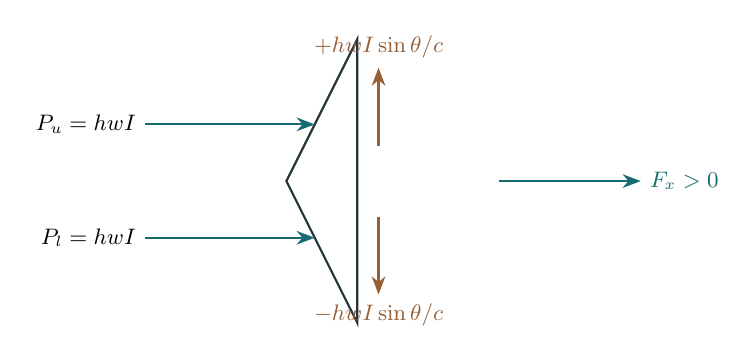
\begin{tikzpicture}[scale=.9,transform shape]
\draw[object] (0,0)--(1,2)--(1,-2)--cycle;
\draw[motion] (-2,.8)--(.4,.8);\draw[motion] (-2,-.8)--(.4,-.8);
\draw[force] (1.3,.5)--(1.3,1.6) node[above] {$+hwI\sin\theta/c$};
\draw[force,color=warm] (1.3,-.5)--(1.3,-1.6) node[below] {$-hwI\sin\theta/c$};
\node[left] at (-2,.8) {$P_u=hwI$};\node[left] at (-2,-.8) {$P_l=hwI$};
\draw[motion] (3,0)--(5,0) node[right] {$F_x>0$};
\end{tikzpicture}
\figcaption{变图近1.2V1\quad 均匀照明的两份竖直反冲相消}
\end{minipage}\end{center}
\item \textbf{小偏转角的力。}固定截获功率$P_u,P_l$，对$\theta\ll1$展开两分力，并说明它们随小角变化的阶数。

由$1-\cos\theta=\theta^2/2+O(\theta^4)$、$\sin\theta=\theta+O(\theta^3)$，
\[
 F_x=\frac{P_u+P_l}{2c}\theta^2+O(\theta^4),\qquad
 F_y=\frac{P_u-P_l}{c}\theta+O(\theta^3).
\]
变图近1.2V2画各自除去功率因子的角系数及首项。横向动量的偏折在一次出现，向前动量的减少在二次出现，所以两分力具有不同的小角阶数。
\begin{center}\begin{minipage}{.98\linewidth}\centering
\begin{tikzpicture}[scale=.88,transform shape]
\draw[axis] (0,0.0)--(7.3,0.0) node[right] {$\theta/{}^\circ$};
\draw[axis] (0,0)--(0,2.8);
\node[above left] at (0,2.8) {角系数};
\draw[thin] (0.000000,0.0)--(0.000000,-0.06);\node[below,font=\scriptsize] at (0.000000,-0.08) {$ 0 $};
\draw[thin] (2.333333,0.0)--(2.333333,-0.06);\node[below,font=\scriptsize] at (2.333333,-0.08) {$ 10 $};
\draw[thin] (4.666667,0.0)--(4.666667,-0.06);\node[below,font=\scriptsize] at (4.666667,-0.08) {$ 20 $};
\draw[thin] (7.000000,0.0)--(7.000000,-0.06);\node[below,font=\scriptsize] at (7.000000,-0.08) {$ 30 $};
\draw[thin] (0,0.000000)--(-.06,0.000000);\node[left,font=\scriptsize] at (-.08,0.000000) {$ 0 $};
\draw[thin] (0,0.446429)--(-.06,0.446429);\node[left,font=\scriptsize] at (-.08,0.446429) {$ 0.1 $};
\draw[thin] (0,1.339286)--(-.06,1.339286);\node[left,font=\scriptsize] at (-.08,1.339286) {$ 0.3 $};
\draw[thin] (0,2.232143)--(-.06,2.232143);\node[left,font=\scriptsize] at (-.08,2.232143) {$ 0.5 $};
\draw[thick,color=accent] plot coordinates {(0.0000000,0.0000000) (0.0291667,0.0000106) (0.0583333,0.0000425) (0.0875000,0.0000956) (0.1166667,0.0001700) (0.1458333,0.0002656) (0.1750000,0.0003825) (0.2041667,0.0005206) (0.2333333,0.0006799) (0.2625000,0.0008605) (0.2916667,0.0010624) (0.3208333,0.0012855) (0.3500000,0.0015298) (0.3791667,0.0017954) (0.4083333,0.0020822) (0.4375000,0.0023902) (0.4666667,0.0027195) (0.4958333,0.0030700) (0.5250000,0.0034418) (0.5541667,0.0038348) (0.5833333,0.0042490) (0.6125000,0.0046845) (0.6416667,0.0051411) (0.6708333,0.0056190) (0.7000000,0.0061181) (0.7291667,0.0066385) (0.7583333,0.0071800) (0.7875000,0.0077428) (0.8166667,0.0083268) (0.8458333,0.0089320) (0.8750000,0.0095584) (0.9041667,0.0102060) (0.9333333,0.0108748) (0.9625000,0.0115648) (0.9916667,0.0122760) (1.0208333,0.0130083) (1.0500000,0.0137619) (1.0791667,0.0145367) (1.1083333,0.0153326) (1.1375000,0.0161497) (1.1666667,0.0169880) (1.1958333,0.0178474) (1.2250000,0.0187280) (1.2541667,0.0196298) (1.2833333,0.0205527) (1.3125000,0.0214968) (1.3416667,0.0224620) (1.3708333,0.0234483) (1.4000000,0.0244558) (1.4291667,0.0254845) (1.4583333,0.0265342) (1.4875000,0.0276051) (1.5166667,0.0286971) (1.5458333,0.0298102) (1.5750000,0.0309444) (1.6041667,0.0320997) (1.6333333,0.0332761) (1.6625000,0.0344736) (1.6916667,0.0356922) (1.7208333,0.0369318) (1.7500000,0.0381926) (1.7791667,0.0394744) (1.8083333,0.0407772) (1.8375000,0.0421012) (1.8666667,0.0434461) (1.8958333,0.0448121) (1.9250000,0.0461992) (1.9541667,0.0476072) (1.9833333,0.0490363) (2.0125000,0.0504864) (2.0416667,0.0519575) (2.0708333,0.0534497) (2.1000000,0.0549628) (2.1291667,0.0564969) (2.1583333,0.0580519) (2.1875000,0.0596280) (2.2166667,0.0612250) (2.2458333,0.0628430) (2.2750000,0.0644819) (2.3041667,0.0661417) (2.3333333,0.0678225) (2.3625000,0.0695242) (2.3916667,0.0712469) (2.4208333,0.0729904) (2.4500000,0.0747549) (2.4791667,0.0765402) (2.5083333,0.0783464) (2.5375000,0.0801735) (2.5666667,0.0820215) (2.5958333,0.0838903) (2.6250000,0.0857800) (2.6541667,0.0876905) (2.6833333,0.0896219) (2.7125000,0.0915740) (2.7416667,0.0935470) (2.7708333,0.0955408) (2.8000000,0.0975554) (2.8291667,0.0995907) (2.8583333,0.1016468) (2.8875000,0.1037237) (2.9166667,0.1058214) (2.9458333,0.1079398) (2.9750000,0.1100789) (3.0041667,0.1122388) (3.0333333,0.1144194) (3.0625000,0.1166206) (3.0916667,0.1188426) (3.1208333,0.1210852) (3.1500000,0.1233486) (3.1791667,0.1256326) (3.2083333,0.1279372) (3.2375000,0.1302625) (3.2666667,0.1326084) (3.2958333,0.1349749) (3.3250000,0.1373620) (3.3541667,0.1397697) (3.3833333,0.1421980) (3.4125000,0.1446469) (3.4416667,0.1471163) (3.4708333,0.1496063) (3.5000000,0.1521168) (3.5291667,0.1546479) (3.5583333,0.1571994) (3.5875000,0.1597715) (3.6166667,0.1623640) (3.6458333,0.1649771) (3.6750000,0.1676106) (3.7041667,0.1702645) (3.7333333,0.1729389) (3.7625000,0.1756337) (3.7916667,0.1783489) (3.8208333,0.1810845) (3.8500000,0.1838405) (3.8791667,0.1866168) (3.9083333,0.1894136) (3.9375000,0.1922306) (3.9666667,0.1950681) (3.9958333,0.1979258) (4.0250000,0.2008038) (4.0541667,0.2037021) (4.0833333,0.2066208) (4.1125000,0.2095596) (4.1416667,0.2125188) (4.1708333,0.2154981) (4.2000000,0.2184977) (4.2291667,0.2215175) (4.2583333,0.2245575) (4.2875000,0.2276176) (4.3166667,0.2306980) (4.3458333,0.2337984) (4.3750000,0.2369191) (4.4041667,0.2400598) (4.4333333,0.2432206) (4.4625000,0.2464016) (4.4916667,0.2496026) (4.5208333,0.2528237) (4.5500000,0.2560648) (4.5791667,0.2593259) (4.6083333,0.2626071) (4.6375000,0.2659082) (4.6666667,0.2692294) (4.6958333,0.2725705) (4.7250000,0.2759315) (4.7541667,0.2793125) (4.7833333,0.2827134) (4.8125000,0.2861343) (4.8416667,0.2895750) (4.8708333,0.2930355) (4.9000000,0.2965160) (4.9291667,0.3000162) (4.9583333,0.3035363) (4.9875000,0.3070762) (5.0166667,0.3106359) (5.0458333,0.3142153) (5.0750000,0.3178145) (5.1041667,0.3214334) (5.1333333,0.3250721) (5.1625000,0.3287304) (5.1916667,0.3324085) (5.2208333,0.3361062) (5.2500000,0.3398235) (5.2791667,0.3435605) (5.3083333,0.3473171) (5.3375000,0.3510933) (5.3666667,0.3548890) (5.3958333,0.3587044) (5.4250000,0.3625392) (5.4541667,0.3663936) (5.4833333,0.3702675) (5.5125000,0.3741609) (5.5416667,0.3780738) (5.5708333,0.3820061) (5.6000000,0.3859578) (5.6291667,0.3899289) (5.6583333,0.3939194) (5.6875000,0.3979294) (5.7166667,0.4019586) (5.7458333,0.4060072) (5.7750000,0.4100751) (5.8041667,0.4141623) (5.8333333,0.4182688) (5.8625000,0.4223945) (5.8916667,0.4265395) (5.9208333,0.4307037) (5.9500000,0.4348871) (5.9791667,0.4390897) (6.0083333,0.4433114) (6.0375000,0.4475523) (6.0666667,0.4518123) (6.0958333,0.4560914) (6.1250000,0.4603895) (6.1541667,0.4647068) (6.1833333,0.4690430) (6.2125000,0.4733983) (6.2416667,0.4777726) (6.2708333,0.4821658) (6.3000000,0.4865780) (6.3291667,0.4910091) (6.3583333,0.4954592) (6.3875000,0.4999281) (6.4166667,0.5044159) (6.4458333,0.5089226) (6.4750000,0.5134480) (6.5041667,0.5179923) (6.5333333,0.5225554) (6.5625000,0.5271372) (6.5916667,0.5317378) (6.6208333,0.5363571) (6.6500000,0.5409950) (6.6791667,0.5456517) (6.7083333,0.5503270) (6.7375000,0.5550209) (6.7666667,0.5597335) (6.7958333,0.5644646) (6.8250000,0.5692143) (6.8541667,0.5739825) (6.8833333,0.5787692) (6.9125000,0.5835744) (6.9416667,0.5883981) (6.9708333,0.5932403) (7.0000000,0.5981009)};
\draw[thick,color=accent] (7.65,2.55)--(8.15,2.55);\node[right,font=\scriptsize] at (8.2,2.55) {$1-\cos\theta$};
\draw[thick,dashed,color=warm] plot coordinates {(0.0000000,0.0000000) (0.0291667,0.0000106) (0.0583333,0.0000425) (0.0875000,0.0000956) (0.1166667,0.0001700) (0.1458333,0.0002656) (0.1750000,0.0003825) (0.2041667,0.0005206) (0.2333333,0.0006799) (0.2625000,0.0008606) (0.2916667,0.0010624) (0.3208333,0.0012855) (0.3500000,0.0015299) (0.3791667,0.0017955) (0.4083333,0.0020823) (0.4375000,0.0023904) (0.4666667,0.0027198) (0.4958333,0.0030704) (0.5250000,0.0034422) (0.5541667,0.0038353) (0.5833333,0.0042497) (0.6125000,0.0046853) (0.6416667,0.0051421) (0.6708333,0.0056202) (0.7000000,0.0061195) (0.7291667,0.0066401) (0.7583333,0.0071820) (0.7875000,0.0077451) (0.8166667,0.0083294) (0.8458333,0.0089350) (0.8750000,0.0095618) (0.9041667,0.0102099) (0.9333333,0.0108792) (0.9625000,0.0115698) (0.9916667,0.0122816) (1.0208333,0.0130147) (1.0500000,0.0137690) (1.0791667,0.0145445) (1.1083333,0.0153414) (1.1375000,0.0161594) (1.1666667,0.0169987) (1.1958333,0.0178593) (1.2250000,0.0187411) (1.2541667,0.0196442) (1.2833333,0.0205685) (1.3125000,0.0215140) (1.3416667,0.0224808) (1.3708333,0.0234689) (1.4000000,0.0244782) (1.4291667,0.0255087) (1.4583333,0.0265605) (1.4875000,0.0276336) (1.5166667,0.0287279) (1.5458333,0.0298434) (1.5750000,0.0309802) (1.6041667,0.0321382) (1.6333333,0.0333175) (1.6625000,0.0345181) (1.6916667,0.0357399) (1.7208333,0.0369829) (1.7500000,0.0382472) (1.7791667,0.0395327) (1.8083333,0.0408395) (1.8375000,0.0421675) (1.8666667,0.0435168) (1.8958333,0.0448873) (1.9250000,0.0462791) (1.9541667,0.0476921) (1.9833333,0.0491264) (2.0125000,0.0505819) (2.0416667,0.0520586) (2.0708333,0.0535567) (2.1000000,0.0550759) (2.1291667,0.0566164) (2.1583333,0.0581782) (2.1875000,0.0597612) (2.2166667,0.0613655) (2.2458333,0.0629910) (2.2750000,0.0646377) (2.3041667,0.0663057) (2.3333333,0.0679950) (2.3625000,0.0697055) (2.3916667,0.0714372) (2.4208333,0.0731902) (2.4500000,0.0749644) (2.4791667,0.0767599) (2.5083333,0.0785767) (2.5375000,0.0804147) (2.5666667,0.0822739) (2.5958333,0.0841544) (2.6250000,0.0860561) (2.6541667,0.0879791) (2.6833333,0.0899233) (2.7125000,0.0918888) (2.7416667,0.0938755) (2.7708333,0.0958835) (2.8000000,0.0979127) (2.8291667,0.0999632) (2.8583333,0.1020349) (2.8875000,0.1041279) (2.9166667,0.1062421) (2.9458333,0.1083776) (2.9750000,0.1105343) (3.0041667,0.1127123) (3.0333333,0.1149115) (3.0625000,0.1171319) (3.0916667,0.1193737) (3.1208333,0.1216366) (3.1500000,0.1239208) (3.1791667,0.1262263) (3.2083333,0.1285530) (3.2375000,0.1309009) (3.2666667,0.1332701) (3.2958333,0.1356606) (3.3250000,0.1380723) (3.3541667,0.1405052) (3.3833333,0.1429594) (3.4125000,0.1454348) (3.4416667,0.1479315) (3.4708333,0.1504495) (3.5000000,0.1529887) (3.5291667,0.1555491) (3.5583333,0.1581308) (3.5875000,0.1607337) (3.6166667,0.1633579) (3.6458333,0.1660033) (3.6750000,0.1686700) (3.7041667,0.1713579) (3.7333333,0.1740671) (3.7625000,0.1767975) (3.7916667,0.1795492) (3.8208333,0.1823221) (3.8500000,0.1851163) (3.8791667,0.1879317) (3.9083333,0.1907684) (3.9375000,0.1936263) (3.9666667,0.1965054) (3.9958333,0.1994058) (4.0250000,0.2023275) (4.0541667,0.2052704) (4.0833333,0.2082346) (4.1125000,0.2112200) (4.1416667,0.2142266) (4.1708333,0.2172545) (4.2000000,0.2203037) (4.2291667,0.2233741) (4.2583333,0.2264657) (4.2875000,0.2295786) (4.3166667,0.2327127) (4.3458333,0.2358681) (4.3750000,0.2390448) (4.4041667,0.2422427) (4.4333333,0.2454618) (4.4625000,0.2487022) (4.4916667,0.2519638) (4.5208333,0.2552467) (4.5500000,0.2585508) (4.5791667,0.2618762) (4.6083333,0.2652228) (4.6375000,0.2685907) (4.6666667,0.2719798) (4.6958333,0.2753902) (4.7250000,0.2788218) (4.7541667,0.2822747) (4.7833333,0.2857488) (4.8125000,0.2892442) (4.8416667,0.2927608) (4.8708333,0.2962987) (4.9000000,0.2998578) (4.9291667,0.3034381) (4.9583333,0.3070397) (4.9875000,0.3106626) (5.0166667,0.3143067) (5.0458333,0.3179721) (5.0750000,0.3216587) (5.1041667,0.3253665) (5.1333333,0.3290956) (5.1625000,0.3328460) (5.1916667,0.3366175) (5.2208333,0.3404104) (5.2500000,0.3442245) (5.2791667,0.3480598) (5.3083333,0.3519164) (5.3375000,0.3557943) (5.3666667,0.3596933) (5.3958333,0.3636137) (5.4250000,0.3675553) (5.4541667,0.3715181) (5.4833333,0.3755022) (5.5125000,0.3795075) (5.5416667,0.3835341) (5.5708333,0.3875819) (5.6000000,0.3916510) (5.6291667,0.3957413) (5.6583333,0.3998529) (5.6875000,0.4039857) (5.7166667,0.4081397) (5.7458333,0.4123151) (5.7750000,0.4165116) (5.8041667,0.4207294) (5.8333333,0.4249685) (5.8625000,0.4292288) (5.8916667,0.4335104) (5.9208333,0.4378132) (5.9500000,0.4421372) (5.9791667,0.4464825) (6.0083333,0.4508491) (6.0375000,0.4552369) (6.0666667,0.4596459) (6.0958333,0.4640762) (6.1250000,0.4685278) (6.1541667,0.4730006) (6.1833333,0.4774946) (6.2125000,0.4820099) (6.2416667,0.4865464) (6.2708333,0.4911042) (6.3000000,0.4956833) (6.3291667,0.5002835) (6.3583333,0.5049051) (6.3875000,0.5095479) (6.4166667,0.5142119) (6.4458333,0.5188972) (6.4750000,0.5236037) (6.5041667,0.5283315) (6.5333333,0.5330805) (6.5625000,0.5378508) (6.5916667,0.5426423) (6.6208333,0.5474550) (6.6500000,0.5522891) (6.6791667,0.5571443) (6.7083333,0.5620208) (6.7375000,0.5669186) (6.7666667,0.5718376) (6.7958333,0.5767779) (6.8250000,0.5817394) (6.8541667,0.5867221) (6.8833333,0.5917261) (6.9125000,0.5967514) (6.9416667,0.6017979) (6.9708333,0.6068656) (7.0000000,0.6119546)};
\draw[thick,dashed,color=warm] (7.65,2.0999999999999996)--(8.15,2.0999999999999996);\node[right,font=\scriptsize] at (8.2,2.0999999999999996) {$\theta^2/2$};
\draw[densely dotted,thick,color=muted] plot coordinates {(0.0000000,0.0000000) (0.0291667,0.0097396) (0.0583333,0.0194791) (0.0875000,0.0292185) (0.1166667,0.0389577) (0.1458333,0.0486968) (0.1750000,0.0584357) (0.2041667,0.0681743) (0.2333333,0.0779125) (0.2625000,0.0876504) (0.2916667,0.0973879) (0.3208333,0.1071249) (0.3500000,0.1168614) (0.3791667,0.1265973) (0.4083333,0.1363326) (0.4375000,0.1460673) (0.4666667,0.1558013) (0.4958333,0.1655346) (0.5250000,0.1752670) (0.5541667,0.1849987) (0.5833333,0.1947294) (0.6125000,0.2044592) (0.6416667,0.2141881) (0.6708333,0.2239159) (0.7000000,0.2336427) (0.7291667,0.2433683) (0.7583333,0.2530928) (0.7875000,0.2628161) (0.8166667,0.2725381) (0.8458333,0.2822589) (0.8750000,0.2919783) (0.9041667,0.3016963) (0.9333333,0.3114128) (0.9625000,0.3211279) (0.9916667,0.3308415) (1.0208333,0.3405535) (1.0500000,0.3502638) (1.0791667,0.3599725) (1.1083333,0.3696795) (1.1375000,0.3793847) (1.1666667,0.3890881) (1.1958333,0.3987897) (1.2250000,0.4084894) (1.2541667,0.4181871) (1.2833333,0.4278828) (1.3125000,0.4375765) (1.3416667,0.4472681) (1.3708333,0.4569576) (1.4000000,0.4666449) (1.4291667,0.4763300) (1.4583333,0.4860128) (1.4875000,0.4956933) (1.5166667,0.5053715) (1.5458333,0.5150472) (1.5750000,0.5247205) (1.6041667,0.5343913) (1.6333333,0.5440596) (1.6625000,0.5537252) (1.6916667,0.5633883) (1.7208333,0.5730486) (1.7500000,0.5827062) (1.7791667,0.5923611) (1.8083333,0.6020131) (1.8375000,0.6116622) (1.8666667,0.6213085) (1.8958333,0.6309518) (1.9250000,0.6405921) (1.9541667,0.6502293) (1.9833333,0.6598634) (2.0125000,0.6694944) (2.0416667,0.6791223) (2.0708333,0.6887468) (2.1000000,0.6983681) (2.1291667,0.7079861) (2.1583333,0.7176007) (2.1875000,0.7272119) (2.2166667,0.7368197) (2.2458333,0.7464239) (2.2750000,0.7560246) (2.3041667,0.7656216) (2.3333333,0.7752151) (2.3625000,0.7848048) (2.3916667,0.7943908) (2.4208333,0.8039731) (2.4500000,0.8135515) (2.4791667,0.8231260) (2.5083333,0.8326966) (2.5375000,0.8422632) (2.5666667,0.8518259) (2.5958333,0.8613845) (2.6250000,0.8709389) (2.6541667,0.8804893) (2.6833333,0.8900354) (2.7125000,0.8995773) (2.7416667,0.9091150) (2.7708333,0.9186483) (2.8000000,0.9281772) (2.8291667,0.9377017) (2.8583333,0.9472218) (2.8875000,0.9567373) (2.9166667,0.9662483) (2.9458333,0.9757547) (2.9750000,0.9852564) (3.0041667,0.9947535) (3.0333333,1.0042458) (3.0625000,1.0137333) (3.0916667,1.0232160) (3.1208333,1.0326939) (3.1500000,1.0421668) (3.1791667,1.0516348) (3.2083333,1.0610977) (3.2375000,1.0705556) (3.2666667,1.0800085) (3.2958333,1.0894561) (3.3250000,1.0988986) (3.3541667,1.1083359) (3.3833333,1.1177679) (3.4125000,1.1271945) (3.4416667,1.1366158) (3.4708333,1.1460317) (3.5000000,1.1554422) (3.5291667,1.1648471) (3.5583333,1.1742465) (3.5875000,1.1836403) (3.6166667,1.1930285) (3.6458333,1.2024110) (3.6750000,1.2117877) (3.7041667,1.2211587) (3.7333333,1.2305239) (3.7625000,1.2398832) (3.7916667,1.2492367) (3.8208333,1.2585842) (3.8500000,1.2679256) (3.8791667,1.2772611) (3.9083333,1.2865905) (3.9375000,1.2959137) (3.9666667,1.3052308) (3.9958333,1.3145417) (4.0250000,1.3238463) (4.0541667,1.3331446) (4.0833333,1.3424366) (4.1125000,1.3517222) (4.1416667,1.3610013) (4.1708333,1.3702740) (4.2000000,1.3795402) (4.2291667,1.3887997) (4.2583333,1.3980527) (4.2875000,1.4072990) (4.3166667,1.4165386) (4.3458333,1.4257715) (4.3750000,1.4349976) (4.4041667,1.4442169) (4.4333333,1.4534293) (4.4625000,1.4626347) (4.4916667,1.4718332) (4.5208333,1.4810247) (4.5500000,1.4902092) (4.5791667,1.4993866) (4.6083333,1.5085568) (4.6375000,1.5177198) (4.6666667,1.5268756) (4.6958333,1.5360242) (4.7250000,1.5451654) (4.7541667,1.5542993) (4.7833333,1.5634258) (4.8125000,1.5725449) (4.8416667,1.5816564) (4.8708333,1.5907605) (4.9000000,1.5998569) (4.9291667,1.6089458) (4.9583333,1.6180270) (4.9875000,1.6271004) (5.0166667,1.6361662) (5.0458333,1.6452241) (5.0750000,1.6542743) (5.1041667,1.6633165) (5.1333333,1.6723509) (5.1625000,1.6813772) (5.1916667,1.6903956) (5.2208333,1.6994059) (5.2500000,1.7084082) (5.2791667,1.7174023) (5.3083333,1.7263882) (5.3375000,1.7353659) (5.3666667,1.7443354) (5.3958333,1.7532965) (5.4250000,1.7622494) (5.4541667,1.7711938) (5.4833333,1.7801298) (5.5125000,1.7890573) (5.5416667,1.7979763) (5.5708333,1.8068867) (5.6000000,1.8157886) (5.6291667,1.8246818) (5.6583333,1.8335663) (5.6875000,1.8424421) (5.7166667,1.8513091) (5.7458333,1.8601673) (5.7750000,1.8690167) (5.8041667,1.8778571) (5.8333333,1.8866887) (5.8625000,1.8955112) (5.8916667,1.9043247) (5.9208333,1.9131292) (5.9500000,1.9219245) (5.9791667,1.9307107) (6.0083333,1.9394878) (6.0375000,1.9482555) (6.0666667,1.9570140) (6.0958333,1.9657632) (6.1250000,1.9745031) (6.1541667,1.9832335) (6.1833333,1.9919545) (6.2125000,2.0006660) (6.2416667,2.0093680) (6.2708333,2.0180605) (6.3000000,2.0267433) (6.3291667,2.0354165) (6.3583333,2.0440800) (6.3875000,2.0527337) (6.4166667,2.0613777) (6.4458333,2.0700119) (6.4750000,2.0786363) (6.5041667,2.0872507) (6.5333333,2.0958552) (6.5625000,2.1044497) (6.5916667,2.1130342) (6.6208333,2.1216087) (6.6500000,2.1301730) (6.6791667,2.1387273) (6.7083333,2.1472713) (6.7375000,2.1558051) (6.7666667,2.1643287) (6.7958333,2.1728419) (6.8250000,2.1813448) (6.8541667,2.1898374) (6.8833333,2.1983195) (6.9125000,2.2067911) (6.9416667,2.2152522) (6.9708333,2.2237028) (7.0000000,2.2321429)};
\draw[densely dotted,thick,color=muted] (7.65,1.65)--(8.15,1.65);\node[right,font=\scriptsize] at (8.2,1.65) {$\sin\theta$};
\draw[thick,color=accent] plot coordinates {(0.0000000,0.0000000) (0.0291667,0.0097396) (0.0583333,0.0194791) (0.0875000,0.0292187) (0.1166667,0.0389582) (0.1458333,0.0486978) (0.1750000,0.0584374) (0.2041667,0.0681769) (0.2333333,0.0779165) (0.2625000,0.0876560) (0.2916667,0.0973956) (0.3208333,0.1071352) (0.3500000,0.1168747) (0.3791667,0.1266143) (0.4083333,0.1363538) (0.4375000,0.1460934) (0.4666667,0.1558330) (0.4958333,0.1655725) (0.5250000,0.1753121) (0.5541667,0.1850517) (0.5833333,0.1947912) (0.6125000,0.2045308) (0.6416667,0.2142703) (0.6708333,0.2240099) (0.7000000,0.2337495) (0.7291667,0.2434890) (0.7583333,0.2532286) (0.7875000,0.2629681) (0.8166667,0.2727077) (0.8458333,0.2824473) (0.8750000,0.2921868) (0.9041667,0.3019264) (0.9333333,0.3116659) (0.9625000,0.3214055) (0.9916667,0.3311451) (1.0208333,0.3408846) (1.0500000,0.3506242) (1.0791667,0.3603637) (1.1083333,0.3701033) (1.1375000,0.3798429) (1.1666667,0.3895824) (1.1958333,0.3993220) (1.2250000,0.4090615) (1.2541667,0.4188011) (1.2833333,0.4285407) (1.3125000,0.4382802) (1.3416667,0.4480198) (1.3708333,0.4577593) (1.4000000,0.4674989) (1.4291667,0.4772385) (1.4583333,0.4869780) (1.4875000,0.4967176) (1.5166667,0.5064571) (1.5458333,0.5161967) (1.5750000,0.5259363) (1.6041667,0.5356758) (1.6333333,0.5454154) (1.6625000,0.5551550) (1.6916667,0.5648945) (1.7208333,0.5746341) (1.7500000,0.5843736) (1.7791667,0.5941132) (1.8083333,0.6038528) (1.8375000,0.6135923) (1.8666667,0.6233319) (1.8958333,0.6330714) (1.9250000,0.6428110) (1.9541667,0.6525506) (1.9833333,0.6622901) (2.0125000,0.6720297) (2.0416667,0.6817692) (2.0708333,0.6915088) (2.1000000,0.7012484) (2.1291667,0.7109879) (2.1583333,0.7207275) (2.1875000,0.7304670) (2.2166667,0.7402066) (2.2458333,0.7499462) (2.2750000,0.7596857) (2.3041667,0.7694253) (2.3333333,0.7791648) (2.3625000,0.7889044) (2.3916667,0.7986440) (2.4208333,0.8083835) (2.4500000,0.8181231) (2.4791667,0.8278626) (2.5083333,0.8376022) (2.5375000,0.8473418) (2.5666667,0.8570813) (2.5958333,0.8668209) (2.6250000,0.8765605) (2.6541667,0.8863000) (2.6833333,0.8960396) (2.7125000,0.9057791) (2.7416667,0.9155187) (2.7708333,0.9252583) (2.8000000,0.9349978) (2.8291667,0.9447374) (2.8583333,0.9544769) (2.8875000,0.9642165) (2.9166667,0.9739561) (2.9458333,0.9836956) (2.9750000,0.9934352) (3.0041667,1.0031747) (3.0333333,1.0129143) (3.0625000,1.0226539) (3.0916667,1.0323934) (3.1208333,1.0421330) (3.1500000,1.0518725) (3.1791667,1.0616121) (3.2083333,1.0713517) (3.2375000,1.0810912) (3.2666667,1.0908308) (3.2958333,1.1005703) (3.3250000,1.1103099) (3.3541667,1.1200495) (3.3833333,1.1297890) (3.4125000,1.1395286) (3.4416667,1.1492681) (3.4708333,1.1590077) (3.5000000,1.1687473) (3.5291667,1.1784868) (3.5583333,1.1882264) (3.5875000,1.1979659) (3.6166667,1.2077055) (3.6458333,1.2174451) (3.6750000,1.2271846) (3.7041667,1.2369242) (3.7333333,1.2466638) (3.7625000,1.2564033) (3.7916667,1.2661429) (3.8208333,1.2758824) (3.8500000,1.2856220) (3.8791667,1.2953616) (3.9083333,1.3051011) (3.9375000,1.3148407) (3.9666667,1.3245802) (3.9958333,1.3343198) (4.0250000,1.3440594) (4.0541667,1.3537989) (4.0833333,1.3635385) (4.1125000,1.3732780) (4.1416667,1.3830176) (4.1708333,1.3927572) (4.2000000,1.4024967) (4.2291667,1.4122363) (4.2583333,1.4219758) (4.2875000,1.4317154) (4.3166667,1.4414550) (4.3458333,1.4511945) (4.3750000,1.4609341) (4.4041667,1.4706736) (4.4333333,1.4804132) (4.4625000,1.4901528) (4.4916667,1.4998923) (4.5208333,1.5096319) (4.5500000,1.5193714) (4.5791667,1.5291110) (4.6083333,1.5388506) (4.6375000,1.5485901) (4.6666667,1.5583297) (4.6958333,1.5680692) (4.7250000,1.5778088) (4.7541667,1.5875484) (4.7833333,1.5972879) (4.8125000,1.6070275) (4.8416667,1.6167671) (4.8708333,1.6265066) (4.9000000,1.6362462) (4.9291667,1.6459857) (4.9583333,1.6557253) (4.9875000,1.6654649) (5.0166667,1.6752044) (5.0458333,1.6849440) (5.0750000,1.6946835) (5.1041667,1.7044231) (5.1333333,1.7141627) (5.1625000,1.7239022) (5.1916667,1.7336418) (5.2208333,1.7433813) (5.2500000,1.7531209) (5.2791667,1.7628605) (5.3083333,1.7726000) (5.3375000,1.7823396) (5.3666667,1.7920791) (5.3958333,1.8018187) (5.4250000,1.8115583) (5.4541667,1.8212978) (5.4833333,1.8310374) (5.5125000,1.8407769) (5.5416667,1.8505165) (5.5708333,1.8602561) (5.6000000,1.8699956) (5.6291667,1.8797352) (5.6583333,1.8894747) (5.6875000,1.8992143) (5.7166667,1.9089539) (5.7458333,1.9186934) (5.7750000,1.9284330) (5.8041667,1.9381726) (5.8333333,1.9479121) (5.8625000,1.9576517) (5.8916667,1.9673912) (5.9208333,1.9771308) (5.9500000,1.9868704) (5.9791667,1.9966099) (6.0083333,2.0063495) (6.0375000,2.0160890) (6.0666667,2.0258286) (6.0958333,2.0355682) (6.1250000,2.0453077) (6.1541667,2.0550473) (6.1833333,2.0647868) (6.2125000,2.0745264) (6.2416667,2.0842660) (6.2708333,2.0940055) (6.3000000,2.1037451) (6.3291667,2.1134846) (6.3583333,2.1232242) (6.3875000,2.1329638) (6.4166667,2.1427033) (6.4458333,2.1524429) (6.4750000,2.1621824) (6.5041667,2.1719220) (6.5333333,2.1816616) (6.5625000,2.1914011) (6.5916667,2.2011407) (6.6208333,2.2108802) (6.6500000,2.2206198) (6.6791667,2.2303594) (6.7083333,2.2400989) (6.7375000,2.2498385) (6.7666667,2.2595780) (6.7958333,2.2693176) (6.8250000,2.2790572) (6.8541667,2.2887967) (6.8833333,2.2985363) (6.9125000,2.3082759) (6.9416667,2.3180154) (6.9708333,2.3277550) (7.0000000,2.3374945)};
\draw[thick,color=accent] (7.65,1.1999999999999997)--(8.15,1.1999999999999997);\node[right,font=\scriptsize] at (8.2,1.1999999999999997) {$\theta$};
\end{tikzpicture}
\figcaption{变图近1.2V2\quad 小偏折的纵向动量减少为二阶，竖直动量为一阶}
\end{minipage}\end{center}
\item \textbf{增加光强后的重力平衡点。}保持主解几何与重力，峰值强度改成指定$y_0=-h/2$平衡所需值的$s$倍。求新的稳定中心段平衡，并说明小振动周期在无重力时怎样变化。

记$v=-y_{\rm eq}/h>0$，中心段向上光力系数为$v/2-v^2/4$。重力固定，原平衡系数为$3/16$，所以$v/2-v^2/4=3/(16s)$。稳定中心段的根为
\[
 v=1-\sqrt{1-\frac{3}{4s}},\qquad s>\frac34.
\]
$s=2$时$v=1-\sqrt{5/8}=0.209430585$，平衡向光轴靠近。$s=3/4$时最大回复力恰等于重力，外段的竖直净力恒为零；更弱光强在指定范围内的最大向上光力小于重力。无重力时$K\propto I_0$，周期$T_0\propto s^{-1/2}$。变图近1.2V3将两种结果分别归一化画出。
\begin{center}\begin{minipage}{.98\linewidth}\centering
\begin{tikzpicture}[scale=.88,transform shape]
\draw[axis] (0,0.0)--(7.3,0.0) node[right] {$s=I_0/I_{0,\rm eq}$};
\draw[axis] (0,0)--(0,2.8);
\node[above left] at (0,2.8) {归一化量};
\draw[thin] (0.000000,0.0)--(0.000000,-0.06);\node[below,font=\scriptsize] at (0.000000,-0.08) {$ 0.76 $};
\draw[thin] (0.750000,0.0)--(0.750000,-0.06);\node[below,font=\scriptsize] at (0.750000,-0.08) {$ 1 $};
\draw[thin] (3.875000,0.0)--(3.875000,-0.06);\node[below,font=\scriptsize] at (3.875000,-0.08) {$ 2 $};
\draw[thin] (7.000000,0.0)--(7.000000,-0.06);\node[below,font=\scriptsize] at (7.000000,-0.08) {$ 3 $};
\draw[thin] (0,0.000000)--(-.06,0.000000);\node[left,font=\scriptsize] at (-.08,0.000000) {$ 0 $};
\draw[thin] (0,1.041667)--(-.06,1.041667);\node[left,font=\scriptsize] at (-.08,1.041667) {$ 0.5 $};
\draw[thin] (0,2.083333)--(-.06,2.083333);\node[left,font=\scriptsize] at (-.08,2.083333) {$ 1 $};
\draw[thick,color=accent] plot coordinates {(0.0000000,1.8443586) (0.0291667,1.7530742) (0.0583333,1.6835989) (0.0875000,1.6258372) (0.1166667,1.5757325) (0.1458333,1.5311599) (0.1750000,1.4908370) (0.2041667,1.4539175) (0.2333333,1.4198065) (0.2625000,1.3880666) (0.2916667,1.3583640) (0.3208333,1.3304374) (0.3500000,1.3040768) (0.3791667,1.2791110) (0.4083333,1.2553973) (0.4375000,1.2328161) (0.4666667,1.2112650) (0.4958333,1.1906562) (0.5250000,1.1709134) (0.5541667,1.1519697) (0.5833333,1.1337664) (0.6125000,1.1162511) (0.6416667,1.0993772) (0.6708333,1.0831030) (0.7000000,1.0673908) (0.7291667,1.0522066) (0.7583333,1.0375193) (0.7875000,1.0233009) (0.8166667,1.0095255) (0.8458333,0.9961693) (0.8750000,0.9832107) (0.9041667,0.9706295) (0.9333333,0.9584072) (0.9625000,0.9465264) (0.9916667,0.9349713) (1.0208333,0.9237268) (1.0500000,0.9127791) (1.0791667,0.9021152) (1.1083333,0.8917229) (1.1375000,0.8815909) (1.1666667,0.8717083) (1.1958333,0.8620653) (1.2250000,0.8526522) (1.2541667,0.8434601) (1.2833333,0.8344807) (1.3125000,0.8257059) (1.3416667,0.8171283) (1.3708333,0.8087406) (1.4000000,0.8005360) (1.4291667,0.7925083) (1.4583333,0.7846512) (1.4875000,0.7769589) (1.5166667,0.7694260) (1.5458333,0.7620472) (1.5750000,0.7548173) (1.6041667,0.7477318) (1.6333333,0.7407860) (1.6625000,0.7339755) (1.6916667,0.7272961) (1.7208333,0.7207439) (1.7500000,0.7143151) (1.7791667,0.7080060) (1.8083333,0.7018131) (1.8375000,0.6957330) (1.8666667,0.6897624) (1.8958333,0.6838984) (1.9250000,0.6781380) (1.9541667,0.6724781) (1.9833333,0.6669162) (2.0125000,0.6614496) (2.0416667,0.6560757) (2.0708333,0.6507921) (2.1000000,0.6455964) (2.1291667,0.6404863) (2.1583333,0.6354596) (2.1875000,0.6305143) (2.2166667,0.6256483) (2.2458333,0.6208596) (2.2750000,0.6161463) (2.3041667,0.6115066) (2.3333333,0.6069386) (2.3625000,0.6024408) (2.3916667,0.5980113) (2.4208333,0.5936487) (2.4500000,0.5893513) (2.4791667,0.5851177) (2.5083333,0.5809464) (2.5375000,0.5768359) (2.5666667,0.5727849) (2.5958333,0.5687922) (2.6250000,0.5648563) (2.6541667,0.5609761) (2.6833333,0.5571503) (2.7125000,0.5533778) (2.7416667,0.5496574) (2.7708333,0.5459880) (2.8000000,0.5423686) (2.8291667,0.5387981) (2.8583333,0.5352755) (2.8875000,0.5317998) (2.9166667,0.5283701) (2.9458333,0.5249854) (2.9750000,0.5216448) (3.0041667,0.5183475) (3.0333333,0.5150925) (3.0625000,0.5118791) (3.0916667,0.5087064) (3.1208333,0.5055737) (3.1500000,0.5024802) (3.1791667,0.4994251) (3.2083333,0.4964077) (3.2375000,0.4934274) (3.2666667,0.4904833) (3.2958333,0.4875749) (3.3250000,0.4847014) (3.3541667,0.4818623) (3.3833333,0.4790568) (3.4125000,0.4762845) (3.4416667,0.4735447) (3.4708333,0.4708368) (3.5000000,0.4681603) (3.5291667,0.4655146) (3.5583333,0.4628991) (3.5875000,0.4603134) (3.6166667,0.4577569) (3.6458333,0.4552291) (3.6750000,0.4527296) (3.7041667,0.4502578) (3.7333333,0.4478133) (3.7625000,0.4453957) (3.7916667,0.4430044) (3.8208333,0.4406391) (3.8500000,0.4382993) (3.8791667,0.4359846) (3.9083333,0.4336945) (3.9375000,0.4314288) (3.9666667,0.4291870) (3.9958333,0.4269687) (4.0250000,0.4247735) (4.0541667,0.4226012) (4.0833333,0.4204512) (4.1125000,0.4183233) (4.1416667,0.4162172) (4.1708333,0.4141324) (4.2000000,0.4120687) (4.2291667,0.4100257) (4.2583333,0.4080032) (4.2875000,0.4060007) (4.3166667,0.4040181) (4.3458333,0.4020550) (4.3750000,0.4001112) (4.4041667,0.3981862) (4.4333333,0.3962800) (4.4625000,0.3943921) (4.4916667,0.3925223) (4.5208333,0.3906704) (4.5500000,0.3888361) (4.5791667,0.3870191) (4.6083333,0.3852192) (4.6375000,0.3834362) (4.6666667,0.3816698) (4.6958333,0.3799198) (4.7250000,0.3781859) (4.7541667,0.3764680) (4.7833333,0.3747658) (4.8125000,0.3730790) (4.8416667,0.3714076) (4.8708333,0.3697512) (4.9000000,0.3681096) (4.9291667,0.3664827) (4.9583333,0.3648703) (4.9875000,0.3632722) (5.0166667,0.3616881) (5.0458333,0.3601179) (5.0750000,0.3585615) (5.1041667,0.3570185) (5.1333333,0.3554889) (5.1625000,0.3539725) (5.1916667,0.3524691) (5.2208333,0.3509785) (5.2500000,0.3495006) (5.2791667,0.3480352) (5.3083333,0.3465821) (5.3375000,0.3451413) (5.3666667,0.3437124) (5.3958333,0.3422955) (5.4250000,0.3408903) (5.4541667,0.3394967) (5.4833333,0.3381145) (5.5125000,0.3367436) (5.5416667,0.3353839) (5.5708333,0.3340353) (5.6000000,0.3326975) (5.6291667,0.3313704) (5.6583333,0.3300541) (5.6875000,0.3287482) (5.7166667,0.3274526) (5.7458333,0.3261674) (5.7750000,0.3248922) (5.8041667,0.3236271) (5.8333333,0.3223719) (5.8625000,0.3211264) (5.8916667,0.3198906) (5.9208333,0.3186643) (5.9500000,0.3174475) (5.9791667,0.3162400) (6.0083333,0.3150417) (6.0375000,0.3138526) (6.0666667,0.3126724) (6.0958333,0.3115011) (6.1250000,0.3103387) (6.1541667,0.3091849) (6.1833333,0.3080398) (6.2125000,0.3069032) (6.2416667,0.3057749) (6.2708333,0.3046550) (6.3000000,0.3035434) (6.3291667,0.3024398) (6.3583333,0.3013444) (6.3875000,0.3002568) (6.4166667,0.2991772) (6.4458333,0.2981053) (6.4750000,0.2970411) (6.5041667,0.2959846) (6.5333333,0.2949356) (6.5625000,0.2938940) (6.5916667,0.2928598) (6.6208333,0.2918330) (6.6500000,0.2908133) (6.6791667,0.2898008) (6.7083333,0.2887953) (6.7375000,0.2877969) (6.7666667,0.2868053) (6.7958333,0.2858206) (6.8250000,0.2848427) (6.8541667,0.2838715) (6.8833333,0.2829070) (6.9125000,0.2819490) (6.9416667,0.2809975) (6.9708333,0.2800524) (7.0000000,0.2791137)};
\draw[thick,color=accent] (7.65,2.55)--(8.15,2.55);\node[right,font=\scriptsize] at (8.2,2.55) {$v_{\rm eq}$};
\draw[thick,dashed,color=warm] plot coordinates {(0.0000000,2.3897472) (0.0291667,2.3752071) (0.0583333,2.3609292) (0.0875000,2.3469058) (0.1166667,2.3331293) (0.1458333,2.3195926) (0.1750000,2.3062888) (0.2041667,2.2932113) (0.2333333,2.2803538) (0.2625000,2.2677101) (0.2916667,2.2552745) (0.3208333,2.2430412) (0.3500000,2.2310049) (0.3791667,2.2191602) (0.4083333,2.2075023) (0.4375000,2.1960262) (0.4666667,2.1847272) (0.4958333,2.1736008) (0.5250000,2.1626427) (0.5541667,2.1518487) (0.5833333,2.1412147) (0.6125000,2.1307368) (0.6416667,2.1204113) (0.6708333,2.1102344) (0.7000000,2.1002027) (0.7291667,2.0903127) (0.7583333,2.0805611) (0.7875000,2.0709447) (0.8166667,2.0614605) (0.8458333,2.0521053) (0.8750000,2.0428764) (0.9041667,2.0337709) (0.9333333,2.0247861) (0.9625000,2.0159193) (0.9916667,2.0071680) (1.0208333,1.9985296) (1.0500000,1.9900019) (1.0791667,1.9815824) (1.1083333,1.9732688) (1.1375000,1.9650591) (1.1666667,1.9569509) (1.1958333,1.9489423) (1.2250000,1.9410312) (1.2541667,1.9332157) (1.2833333,1.9254939) (1.3125000,1.9178638) (1.3416667,1.9103237) (1.3708333,1.9028719) (1.4000000,1.8955066) (1.4291667,1.8882261) (1.4583333,1.8810290) (1.4875000,1.8739134) (1.5166667,1.8668781) (1.5458333,1.8599214) (1.5750000,1.8530418) (1.6041667,1.8462381) (1.6333333,1.8395088) (1.6625000,1.8328525) (1.6916667,1.8262679) (1.7208333,1.8197538) (1.7500000,1.8133089) (1.7791667,1.8069320) (1.8083333,1.8006219) (1.8375000,1.7943775) (1.8666667,1.7881976) (1.8958333,1.7820811) (1.9250000,1.7760269) (1.9541667,1.7700340) (1.9833333,1.7641014) (2.0125000,1.7582281) (2.0416667,1.7524130) (2.0708333,1.7466552) (2.1000000,1.7409538) (2.1291667,1.7353079) (2.1583333,1.7297166) (2.1875000,1.7241789) (2.2166667,1.7186941) (2.2458333,1.7132614) (2.2750000,1.7078798) (2.3041667,1.7025486) (2.3333333,1.6972670) (2.3625000,1.6920343) (2.3916667,1.6868497) (2.4208333,1.6817124) (2.4500000,1.6766218) (2.4791667,1.6715772) (2.5083333,1.6665778) (2.5375000,1.6616230) (2.5666667,1.6567121) (2.5958333,1.6518445) (2.6250000,1.6470196) (2.6541667,1.6422367) (2.6833333,1.6374953) (2.7125000,1.6327946) (2.7416667,1.6281342) (2.7708333,1.6235135) (2.8000000,1.6189320) (2.8291667,1.6143889) (2.8583333,1.6098840) (2.8875000,1.6054165) (2.9166667,1.6009860) (2.9458333,1.5965920) (2.9750000,1.5922340) (3.0041667,1.5879114) (3.0333333,1.5836239) (3.0625000,1.5793709) (3.0916667,1.5751520) (3.1208333,1.5709668) (3.1500000,1.5668147) (3.1791667,1.5626953) (3.2083333,1.5586083) (3.2375000,1.5545532) (3.2666667,1.5505296) (3.2958333,1.5465371) (3.3250000,1.5425752) (3.3541667,1.5386436) (3.3833333,1.5347420) (3.4125000,1.5308699) (3.4416667,1.5270269) (3.4708333,1.5232127) (3.5000000,1.5194270) (3.5291667,1.5156694) (3.5583333,1.5119395) (3.5875000,1.5082370) (3.6166667,1.5045615) (3.6458333,1.5009128) (3.6750000,1.4972906) (3.7041667,1.4936944) (3.7333333,1.4901240) (3.7625000,1.4865791) (3.7916667,1.4830594) (3.8208333,1.4795645) (3.8500000,1.4760943) (3.8791667,1.4726483) (3.9083333,1.4692264) (3.9375000,1.4658282) (3.9666667,1.4624535) (3.9958333,1.4591020) (4.0250000,1.4557734) (4.0541667,1.4524675) (4.0833333,1.4491840) (4.1125000,1.4459227) (4.1416667,1.4426834) (4.1708333,1.4394656) (4.2000000,1.4362694) (4.2291667,1.4330943) (4.2583333,1.4299402) (4.2875000,1.4268068) (4.3166667,1.4236939) (4.3458333,1.4206013) (4.3750000,1.4175288) (4.4041667,1.4144761) (4.4333333,1.4114431) (4.4625000,1.4084295) (4.4916667,1.4054351) (4.5208333,1.4024597) (4.5500000,1.3995032) (4.5791667,1.3965652) (4.6083333,1.3936457) (4.6375000,1.3907445) (4.6666667,1.3878612) (4.6958333,1.3849959) (4.7250000,1.3821482) (4.7541667,1.3793180) (4.7833333,1.3765051) (4.8125000,1.3737093) (4.8416667,1.3709305) (4.8708333,1.3681686) (4.9000000,1.3654232) (4.9291667,1.3626943) (4.9583333,1.3599817) (4.9875000,1.3572852) (5.0166667,1.3546047) (5.0458333,1.3519401) (5.0750000,1.3492910) (5.1041667,1.3466575) (5.1333333,1.3440394) (5.1625000,1.3414365) (5.1916667,1.3388486) (5.2208333,1.3362757) (5.2500000,1.3337175) (5.2791667,1.3311740) (5.3083333,1.3286449) (5.3375000,1.3261303) (5.3666667,1.3236298) (5.3958333,1.3211435) (5.4250000,1.3186711) (5.4541667,1.3162125) (5.4833333,1.3137676) (5.5125000,1.3113363) (5.5416667,1.3089185) (5.5708333,1.3065139) (5.6000000,1.3041226) (5.6291667,1.3017444) (5.6583333,1.2993791) (5.6875000,1.2970267) (5.7166667,1.2946870) (5.7458333,1.2923599) (5.7750000,1.2900453) (5.8041667,1.2877431) (5.8333333,1.2854532) (5.8625000,1.2831755) (5.8916667,1.2809098) (5.9208333,1.2786561) (5.9500000,1.2764143) (5.9791667,1.2741842) (6.0083333,1.2719657) (6.0375000,1.2697588) (6.0666667,1.2675634) (6.0958333,1.2653792) (6.1250000,1.2632064) (6.1541667,1.2610447) (6.1833333,1.2588940) (6.2125000,1.2567544) (6.2416667,1.2546255) (6.2708333,1.2525075) (6.3000000,1.2504002) (6.3291667,1.2483035) (6.3583333,1.2462172) (6.3875000,1.2441414) (6.4166667,1.2420760) (6.4458333,1.2400208) (6.4750000,1.2379758) (6.5041667,1.2359408) (6.5333333,1.2339159) (6.5625000,1.2319008) (6.5916667,1.2298956) (6.6208333,1.2279002) (6.6500000,1.2259145) (6.6791667,1.2239383) (6.7083333,1.2219717) (6.7375000,1.2200145) (6.7666667,1.2180667) (6.7958333,1.2161282) (6.8250000,1.2141990) (6.8541667,1.2122789) (6.8833333,1.2103678) (6.9125000,1.2084658) (6.9416667,1.2065727) (6.9708333,1.2046885) (7.0000000,1.2028131)};
\draw[thick,dashed,color=warm] (7.65,2.0999999999999996)--(8.15,2.0999999999999996);\node[right,font=\scriptsize] at (8.2,2.0999999999999996) {$T_0(s)/T_0(1)$};
\end{tikzpicture}
\figcaption{变图近1.2V3\quad 提高光强使重力平衡靠近光轴，无重力周期按平方根缩短}
\end{minipage}\end{center}
\item \textbf{小有限振幅的周期修正。}由$\ddot y+\Omega_0^2y-\Omega_0^2y|y|/(2h)=0$，求振幅$a\ll h$的频率首项。

取$y\simeq a\cos\Omega t$，$|\cos t|\cos t$的基频系数为
\[
 \frac1\pi\int_{-\pi}^{\pi}|\cos t|\cos^2t\,\dd t
 =\frac8{3\pi}.
\]
将基频系数相等，得$\Omega^2/\Omega_0^2\simeq1-4a/(3\pi h)$，所以
\[
 \Omega/\Omega_0\simeq1-\frac{2a}{3\pi h},\qquad
 T/T_0\simeq1+\frac{2a}{3\pi h}.
\]
在$a/h=0.05$时首阶周期增加1.06103\%。变图近1.2V4把能量积分给的周期比与首阶近似并列，展示软回复力随振幅的修正。
\begin{center}\begin{minipage}{.98\linewidth}\centering
\begin{tikzpicture}[scale=.88,transform shape]
\draw[axis] (0,0)--(7.3,0) node[right] {$A=a/h$};
\draw[axis] (0,0)--(0,2.8);
\node[above left] at (0,2.8) {$T/T_0$};
\draw[thin] (0.000000,0)--(0.000000,-0.06);\node[below,font=\scriptsize] at (0.000000,-0.08) {$ 0 $};
\draw[thin] (1.750000,0)--(1.750000,-0.06);\node[below,font=\scriptsize] at (1.750000,-0.08) {$ 0.05 $};
\draw[thin] (3.500000,0)--(3.500000,-0.06);\node[below,font=\scriptsize] at (3.500000,-0.08) {$ 0.1 $};
\draw[thin] (7.000000,0)--(7.000000,-0.06);\node[below,font=\scriptsize] at (7.000000,-0.08) {$ 0.2 $};
\draw[thin] (0,0.000000)--(-.06,0.000000);\node[left,font=\scriptsize] at (-.08,0.000000) {$ 1 $};
\draw[thin] (0,0.442083)--(-.06,0.442083);\node[left,font=\scriptsize] at (-.08,0.442083) {$ 1.01061 $};
\draw[thin] (0,1.250000)--(-.06,1.250000);\node[left,font=\scriptsize] at (-.08,1.250000) {$ 1.03 $};
\draw[thin] (0,2.500000)--(-.06,2.500000);\node[left,font=\scriptsize] at (-.08,2.500000) {$ 1.06 $};
\draw[thick,color=accent] plot coordinates {(0.0000000,0.0000000) (0.0291667,0.0073703) (0.0583333,0.0147445) (0.0875000,0.0221228) (0.1166667,0.0295050) (0.1458333,0.0368913) (0.1750000,0.0442815) (0.2041667,0.0516757) (0.2333333,0.0590740) (0.2625000,0.0664763) (0.2916667,0.0738825) (0.3208333,0.0812928) (0.3500000,0.0887071) (0.3791667,0.0961255) (0.4083333,0.1035478) (0.4375000,0.1109742) (0.4666667,0.1184047) (0.4958333,0.1258392) (0.5250000,0.1332777) (0.5541667,0.1407202) (0.5833333,0.1481669) (0.6125000,0.1556175) (0.6416667,0.1630723) (0.6708333,0.1705311) (0.7000000,0.1779939) (0.7291667,0.1854609) (0.7583333,0.1929319) (0.7875000,0.2004070) (0.8166667,0.2078861) (0.8458333,0.2153694) (0.8750000,0.2228567) (0.9041667,0.2303482) (0.9333333,0.2378437) (0.9625000,0.2453433) (0.9916667,0.2528471) (1.0208333,0.2603549) (1.0500000,0.2678669) (1.0791667,0.2753830) (1.1083333,0.2829032) (1.1375000,0.2904275) (1.1666667,0.2979559) (1.1958333,0.3054885) (1.2250000,0.3130252) (1.2541667,0.3205661) (1.2833333,0.3281111) (1.3125000,0.3356602) (1.3416667,0.3432135) (1.3708333,0.3507709) (1.4000000,0.3583325) (1.4291667,0.3658983) (1.4583333,0.3734682) (1.4875000,0.3810423) (1.5166667,0.3886206) (1.5458333,0.3962031) (1.5750000,0.4037897) (1.6041667,0.4113805) (1.6333333,0.4189755) (1.6625000,0.4265747) (1.6916667,0.4341781) (1.7208333,0.4417857) (1.7500000,0.4493975) (1.7791667,0.4570135) (1.8083333,0.4646338) (1.8375000,0.4722582) (1.8666667,0.4798869) (1.8958333,0.4875198) (1.9250000,0.4951569) (1.9541667,0.5027982) (1.9833333,0.5104438) (2.0125000,0.5180936) (2.0416667,0.5257477) (2.0708333,0.5334060) (2.1000000,0.5410686) (2.1291667,0.5487355) (2.1583333,0.5564065) (2.1875000,0.5640819) (2.2166667,0.5717615) (2.2458333,0.5794454) (2.2750000,0.5871336) (2.3041667,0.5948261) (2.3333333,0.6025228) (2.3625000,0.6102238) (2.3916667,0.6179292) (2.4208333,0.6256388) (2.4500000,0.6333527) (2.4791667,0.6410709) (2.5083333,0.6487935) (2.5375000,0.6565203) (2.5666667,0.6642515) (2.5958333,0.6719870) (2.6250000,0.6797268) (2.6541667,0.6874710) (2.6833333,0.6952194) (2.7125000,0.7029723) (2.7416667,0.7107294) (2.7708333,0.7184909) (2.8000000,0.7262568) (2.8291667,0.7340270) (2.8583333,0.7418016) (2.8875000,0.7495805) (2.9166667,0.7573638) (2.9458333,0.7651515) (2.9750000,0.7729435) (3.0041667,0.7807400) (3.0333333,0.7885408) (3.0625000,0.7963460) (3.0916667,0.8041556) (3.1208333,0.8119695) (3.1500000,0.8197879) (3.1791667,0.8276107) (3.2083333,0.8354379) (3.2375000,0.8432695) (3.2666667,0.8511056) (3.2958333,0.8589460) (3.3250000,0.8667909) (3.3541667,0.8746402) (3.3833333,0.8824940) (3.4125000,0.8903522) (3.4416667,0.8982148) (3.4708333,0.9060819) (3.5000000,0.9139534) (3.5291667,0.9218294) (3.5583333,0.9297098) (3.5875000,0.9375947) (3.6166667,0.9454841) (3.6458333,0.9533779) (3.6750000,0.9612762) (3.7041667,0.9691791) (3.7333333,0.9770863) (3.7625000,0.9849981) (3.7916667,0.9929144) (3.8208333,1.0008352) (3.8500000,1.0087604) (3.8791667,1.0166902) (3.9083333,1.0246245) (3.9375000,1.0325633) (3.9666667,1.0405067) (3.9958333,1.0484545) (4.0250000,1.0564069) (4.0541667,1.0643638) (4.0833333,1.0723253) (4.1125000,1.0802913) (4.1416667,1.0882619) (4.1708333,1.0962370) (4.2000000,1.1042166) (4.2291667,1.1122008) (4.2583333,1.1201896) (4.2875000,1.1281830) (4.3166667,1.1361809) (4.3458333,1.1441834) (4.3750000,1.1521905) (4.4041667,1.1602021) (4.4333333,1.1682184) (4.4625000,1.1762392) (4.4916667,1.1842647) (4.5208333,1.1922948) (4.5500000,1.2003294) (4.5791667,1.2083687) (4.6083333,1.2164126) (4.6375000,1.2244611) (4.6666667,1.2325143) (4.6958333,1.2405721) (4.7250000,1.2486345) (4.7541667,1.2567016) (4.7833333,1.2647733) (4.8125000,1.2728496) (4.8416667,1.2809306) (4.8708333,1.2890163) (4.9000000,1.2971066) (4.9291667,1.3052016) (4.9583333,1.3133013) (4.9875000,1.3214057) (5.0166667,1.3295147) (5.0458333,1.3376284) (5.0750000,1.3457468) (5.1041667,1.3538699) (5.1333333,1.3619977) (5.1625000,1.3701302) (5.1916667,1.3782675) (5.2208333,1.3864094) (5.2500000,1.3945561) (5.2791667,1.4027074) (5.3083333,1.4108635) (5.3375000,1.4190244) (5.3666667,1.4271899) (5.3958333,1.4353603) (5.4250000,1.4435353) (5.4541667,1.4517151) (5.4833333,1.4598997) (5.5125000,1.4680890) (5.5416667,1.4762831) (5.5708333,1.4844820) (5.6000000,1.4926856) (5.6291667,1.5008941) (5.6583333,1.5091073) (5.6875000,1.5173253) (5.7166667,1.5255481) (5.7458333,1.5337757) (5.7750000,1.5420080) (5.8041667,1.5502452) (5.8333333,1.5584873) (5.8625000,1.5667341) (5.8916667,1.5749857) (5.9208333,1.5832422) (5.9500000,1.5915035) (5.9791667,1.5997697) (6.0083333,1.6080407) (6.0375000,1.6163165) (6.0666667,1.6245972) (6.0958333,1.6328827) (6.1250000,1.6411731) (6.1541667,1.6494684) (6.1833333,1.6577686) (6.2125000,1.6660736) (6.2416667,1.6743835) (6.2708333,1.6826983) (6.3000000,1.6910179) (6.3291667,1.6993425) (6.3583333,1.7076720) (6.3875000,1.7160064) (6.4166667,1.7243456) (6.4458333,1.7326898) (6.4750000,1.7410390) (6.5041667,1.7493930) (6.5333333,1.7577520) (6.5625000,1.7661159) (6.5916667,1.7744847) (6.6208333,1.7828585) (6.6500000,1.7912373) (6.6791667,1.7996210) (6.7083333,1.8080096) (6.7375000,1.8164032) (6.7666667,1.8248018) (6.7958333,1.8332054) (6.8250000,1.8416139) (6.8541667,1.8500274) (6.8833333,1.8584460) (6.9125000,1.8668695) (6.9416667,1.8752980) (6.9708333,1.8837315) (7.0000000,1.8921700)};
\draw[thick,color=accent] (7.65,2.55)--(8.15,2.55);\node[right,font=\scriptsize] at (8.2,2.55) {能量积分};
\draw[thick,dashed,color=warm] plot coordinates {(0.0000000,0.0000000) (0.0291667,0.0073683) (0.0583333,0.0147366) (0.0875000,0.0221049) (0.1166667,0.0294731) (0.1458333,0.0368414) (0.1750000,0.0442097) (0.2041667,0.0515780) (0.2333333,0.0589463) (0.2625000,0.0663146) (0.2916667,0.0736828) (0.3208333,0.0810511) (0.3500000,0.0884194) (0.3791667,0.0957877) (0.4083333,0.1031560) (0.4375000,0.1105243) (0.4666667,0.1178926) (0.4958333,0.1252608) (0.5250000,0.1326291) (0.5541667,0.1399974) (0.5833333,0.1473657) (0.6125000,0.1547340) (0.6416667,0.1621023) (0.6708333,0.1694705) (0.7000000,0.1768388) (0.7291667,0.1842071) (0.7583333,0.1915754) (0.7875000,0.1989437) (0.8166667,0.2063120) (0.8458333,0.2136802) (0.8750000,0.2210485) (0.9041667,0.2284168) (0.9333333,0.2357851) (0.9625000,0.2431534) (0.9916667,0.2505217) (1.0208333,0.2578900) (1.0500000,0.2652582) (1.0791667,0.2726265) (1.1083333,0.2799948) (1.1375000,0.2873631) (1.1666667,0.2947314) (1.1958333,0.3020997) (1.2250000,0.3094679) (1.2541667,0.3168362) (1.2833333,0.3242045) (1.3125000,0.3315728) (1.3416667,0.3389411) (1.3708333,0.3463094) (1.4000000,0.3536777) (1.4291667,0.3610459) (1.4583333,0.3684142) (1.4875000,0.3757825) (1.5166667,0.3831508) (1.5458333,0.3905191) (1.5750000,0.3978874) (1.6041667,0.4052556) (1.6333333,0.4126239) (1.6625000,0.4199922) (1.6916667,0.4273605) (1.7208333,0.4347288) (1.7500000,0.4420971) (1.7791667,0.4494653) (1.8083333,0.4568336) (1.8375000,0.4642019) (1.8666667,0.4715702) (1.8958333,0.4789385) (1.9250000,0.4863068) (1.9541667,0.4936751) (1.9833333,0.5010433) (2.0125000,0.5084116) (2.0416667,0.5157799) (2.0708333,0.5231482) (2.1000000,0.5305165) (2.1291667,0.5378848) (2.1583333,0.5452530) (2.1875000,0.5526213) (2.2166667,0.5599896) (2.2458333,0.5673579) (2.2750000,0.5747262) (2.3041667,0.5820945) (2.3333333,0.5894628) (2.3625000,0.5968310) (2.3916667,0.6041993) (2.4208333,0.6115676) (2.4500000,0.6189359) (2.4791667,0.6263042) (2.5083333,0.6336725) (2.5375000,0.6410407) (2.5666667,0.6484090) (2.5958333,0.6557773) (2.6250000,0.6631456) (2.6541667,0.6705139) (2.6833333,0.6778822) (2.7125000,0.6852504) (2.7416667,0.6926187) (2.7708333,0.6999870) (2.8000000,0.7073553) (2.8291667,0.7147236) (2.8583333,0.7220919) (2.8875000,0.7294602) (2.9166667,0.7368284) (2.9458333,0.7441967) (2.9750000,0.7515650) (3.0041667,0.7589333) (3.0333333,0.7663016) (3.0625000,0.7736699) (3.0916667,0.7810381) (3.1208333,0.7884064) (3.1500000,0.7957747) (3.1791667,0.8031430) (3.2083333,0.8105113) (3.2375000,0.8178796) (3.2666667,0.8252479) (3.2958333,0.8326161) (3.3250000,0.8399844) (3.3541667,0.8473527) (3.3833333,0.8547210) (3.4125000,0.8620893) (3.4416667,0.8694576) (3.4708333,0.8768258) (3.5000000,0.8841941) (3.5291667,0.8915624) (3.5583333,0.8989307) (3.5875000,0.9062990) (3.6166667,0.9136673) (3.6458333,0.9210356) (3.6750000,0.9284038) (3.7041667,0.9357721) (3.7333333,0.9431404) (3.7625000,0.9505087) (3.7916667,0.9578770) (3.8208333,0.9652453) (3.8500000,0.9726135) (3.8791667,0.9799818) (3.9083333,0.9873501) (3.9375000,0.9947184) (3.9666667,1.0020867) (3.9958333,1.0094550) (4.0250000,1.0168232) (4.0541667,1.0241915) (4.0833333,1.0315598) (4.1125000,1.0389281) (4.1416667,1.0462964) (4.1708333,1.0536647) (4.2000000,1.0610330) (4.2291667,1.0684012) (4.2583333,1.0757695) (4.2875000,1.0831378) (4.3166667,1.0905061) (4.3458333,1.0978744) (4.3750000,1.1052427) (4.4041667,1.1126109) (4.4333333,1.1199792) (4.4625000,1.1273475) (4.4916667,1.1347158) (4.5208333,1.1420841) (4.5500000,1.1494524) (4.5791667,1.1568207) (4.6083333,1.1641889) (4.6375000,1.1715572) (4.6666667,1.1789255) (4.6958333,1.1862938) (4.7250000,1.1936621) (4.7541667,1.2010304) (4.7833333,1.2083986) (4.8125000,1.2157669) (4.8416667,1.2231352) (4.8708333,1.2305035) (4.9000000,1.2378718) (4.9291667,1.2452401) (4.9583333,1.2526083) (4.9875000,1.2599766) (5.0166667,1.2673449) (5.0458333,1.2747132) (5.0750000,1.2820815) (5.1041667,1.2894498) (5.1333333,1.2968181) (5.1625000,1.3041863) (5.1916667,1.3115546) (5.2208333,1.3189229) (5.2500000,1.3262912) (5.2791667,1.3336595) (5.3083333,1.3410278) (5.3375000,1.3483960) (5.3666667,1.3557643) (5.3958333,1.3631326) (5.4250000,1.3705009) (5.4541667,1.3778692) (5.4833333,1.3852375) (5.5125000,1.3926058) (5.5416667,1.3999740) (5.5708333,1.4073423) (5.6000000,1.4147106) (5.6291667,1.4220789) (5.6583333,1.4294472) (5.6875000,1.4368155) (5.7166667,1.4441837) (5.7458333,1.4515520) (5.7750000,1.4589203) (5.8041667,1.4662886) (5.8333333,1.4736569) (5.8625000,1.4810252) (5.8916667,1.4883934) (5.9208333,1.4957617) (5.9500000,1.5031300) (5.9791667,1.5104983) (6.0083333,1.5178666) (6.0375000,1.5252349) (6.0666667,1.5326032) (6.0958333,1.5399714) (6.1250000,1.5473397) (6.1541667,1.5547080) (6.1833333,1.5620763) (6.2125000,1.5694446) (6.2416667,1.5768129) (6.2708333,1.5841811) (6.3000000,1.5915494) (6.3291667,1.5989177) (6.3583333,1.6062860) (6.3875000,1.6136543) (6.4166667,1.6210226) (6.4458333,1.6283909) (6.4750000,1.6357591) (6.5041667,1.6431274) (6.5333333,1.6504957) (6.5625000,1.6578640) (6.5916667,1.6652323) (6.6208333,1.6726006) (6.6500000,1.6799688) (6.6791667,1.6873371) (6.7083333,1.6947054) (6.7375000,1.7020737) (6.7666667,1.7094420) (6.7958333,1.7168103) (6.8250000,1.7241786) (6.8541667,1.7315468) (6.8833333,1.7389151) (6.9125000,1.7462834) (6.9416667,1.7536517) (6.9708333,1.7610200) (7.0000000,1.7683883)};
\draw[thick,dashed,color=warm] (7.65,2.0999999999999996)--(8.15,2.0999999999999996);\node[right,font=\scriptsize] at (8.2,2.0999999999999996) {$1+2A/(3\pi)$};
\end{tikzpicture}
\figcaption{变图近1.2V4\quad 有限振幅能量积分与首阶软化修正}
\end{minipage}\end{center}
\item \textbf{重力平衡附近的小振动。}已在$y_{\rm eq}=-vh$、$0<v<1$处用光力平衡重力，求该位置附近的小振动周期。

对负位移，$F_y=-Ky(1+y/(2h))$，求导得$F'_y=-K(1+y/h)$。在$y=-vh$处，令$\eta=y-y_{\rm eq}$，常量光力与重力相消，线性项为$-K(1-v)\eta$。故
\[
 \Omega_{\rm eq}=\sqrt{\frac{K(1-v)}m},\qquad
 T_{\rm eq}=\frac{T_0}{\sqrt{1-v}}.
\]
变图近1.2V5画周期比，在$v=1/2$为$\sqrt2$。这里$T_0$采用同一峰值强度下的中心回复系数，平衡越接近常力外段，局部回复斜率越小。
\begin{center}\begin{minipage}{.98\linewidth}\centering
\begin{tikzpicture}[scale=.88,transform shape]
\draw[axis] (0,0.0)--(7.3,0.0) node[right] {$v=-y_{\rm eq}/h$};
\draw[axis] (0,0)--(0,2.8);
\node[above left] at (0,2.8) {$T_{\rm eq}/T_0$};
\draw[thin] (0.000000,0.0)--(0.000000,-0.06);\node[below,font=\scriptsize] at (0.000000,-0.08) {$ 0 $};
\draw[thin] (3.888889,0.0)--(3.888889,-0.06);\node[below,font=\scriptsize] at (3.888889,-0.08) {$ 0.5 $};
\draw[thin] (5.833333,0.0)--(5.833333,-0.06);\node[below,font=\scriptsize] at (5.833333,-0.08) {$ 0.75 $};
\draw[thin] (7.000000,0.0)--(7.000000,-0.06);\node[below,font=\scriptsize] at (7.000000,-0.08) {$ 0.9 $};
\draw[thin] (0,0.000000)--(-.06,0.000000);\node[left,font=\scriptsize] at (-.08,0.000000) {$ 0 $};
\draw[thin] (0,0.757576)--(-.06,0.757576);\node[left,font=\scriptsize] at (-.08,0.757576) {$ 1 $};
\draw[thin] (0,1.071371)--(-.06,1.071371);\node[left,font=\scriptsize] at (-.08,1.071371) {$ 1.41421 $};
\draw[thin] (0,2.272727)--(-.06,2.272727);\node[left,font=\scriptsize] at (-.08,2.272727) {$ 3 $};
\draw[thick,color=accent] plot coordinates {(0.0000000,0.7575758) (0.0291667,0.7590002) (0.0583333,0.7604327) (0.0875000,0.7618734) (0.1166667,0.7633223) (0.1458333,0.7647795) (0.1750000,0.7662451) (0.2041667,0.7677191) (0.2333333,0.7692016) (0.2625000,0.7706928) (0.2916667,0.7721927) (0.3208333,0.7737014) (0.3500000,0.7752190) (0.3791667,0.7767455) (0.4083333,0.7782811) (0.4375000,0.7798258) (0.4666667,0.7813797) (0.4958333,0.7829430) (0.5250000,0.7845157) (0.5541667,0.7860979) (0.5833333,0.7876898) (0.6125000,0.7892913) (0.6416667,0.7909027) (0.6708333,0.7925239) (0.7000000,0.7941552) (0.7291667,0.7957966) (0.7583333,0.7974482) (0.7875000,0.7991101) (0.8166667,0.8007825) (0.8458333,0.8024654) (0.8750000,0.8041589) (0.9041667,0.8058633) (0.9333333,0.8075785) (0.9625000,0.8093047) (0.9916667,0.8110420) (1.0208333,0.8127906) (1.0500000,0.8145505) (1.0791667,0.8163219) (1.1083333,0.8181049) (1.1375000,0.8198997) (1.1666667,0.8217063) (1.1958333,0.8235249) (1.2250000,0.8253556) (1.2541667,0.8271986) (1.2833333,0.8290540) (1.3125000,0.8309220) (1.3416667,0.8328026) (1.3708333,0.8346960) (1.4000000,0.8366025) (1.4291667,0.8385220) (1.4583333,0.8404548) (1.4875000,0.8424011) (1.5166667,0.8443609) (1.5458333,0.8463345) (1.5750000,0.8483220) (1.6041667,0.8503235) (1.6333333,0.8523393) (1.6625000,0.8543695) (1.6916667,0.8564143) (1.7208333,0.8584738) (1.7500000,0.8605482) (1.7791667,0.8626378) (1.8083333,0.8647426) (1.8375000,0.8668630) (1.8666667,0.8689990) (1.8958333,0.8711509) (1.9250000,0.8733188) (1.9541667,0.8755030) (1.9833333,0.8777037) (2.0125000,0.8799211) (2.0416667,0.8821553) (2.0708333,0.8844067) (2.1000000,0.8866754) (2.1291667,0.8889616) (2.1583333,0.8912656) (2.1875000,0.8935876) (2.2166667,0.8959279) (2.2458333,0.8982866) (2.2750000,0.9006641) (2.3041667,0.9030605) (2.3333333,0.9054762) (2.3625000,0.9079114) (2.3916667,0.9103663) (2.4208333,0.9128413) (2.4500000,0.9153365) (2.4791667,0.9178523) (2.5083333,0.9203890) (2.5375000,0.9229468) (2.5666667,0.9255261) (2.5958333,0.9281271) (2.6250000,0.9307502) (2.6541667,0.9333956) (2.6833333,0.9360637) (2.7125000,0.9387549) (2.7416667,0.9414693) (2.7708333,0.9442075) (2.8000000,0.9469697) (2.8291667,0.9497563) (2.8583333,0.9525676) (2.8875000,0.9554040) (2.9166667,0.9582660) (2.9458333,0.9611538) (2.9750000,0.9640678) (3.0041667,0.9670086) (3.0333333,0.9699764) (3.0625000,0.9729717) (3.0916667,0.9759949) (3.1208333,0.9790465) (3.1500000,0.9821269) (3.1791667,0.9852365) (3.2083333,0.9883759) (3.2375000,0.9915454) (3.2666667,0.9947457) (3.2958333,0.9979772) (3.3250000,1.0012403) (3.3541667,1.0045357) (3.3833333,1.0078638) (3.4125000,1.0112252) (3.4416667,1.0146205) (3.4708333,1.0180502) (3.5000000,1.0215149) (3.5291667,1.0250153) (3.5583333,1.0285519) (3.5875000,1.0321253) (3.6166667,1.0357363) (3.6458333,1.0393854) (3.6750000,1.0430733) (3.7041667,1.0468008) (3.7333333,1.0505686) (3.7625000,1.0543773) (3.7916667,1.0582277) (3.8208333,1.0621207) (3.8500000,1.0660569) (3.8791667,1.0700372) (3.9083333,1.0740624) (3.9375000,1.0781334) (3.9666667,1.0822511) (3.9958333,1.0864163) (4.0250000,1.0906299) (4.0541667,1.0948930) (4.0833333,1.0992064) (4.1125000,1.1035713) (4.1416667,1.1079885) (4.1708333,1.1124592) (4.2000000,1.1169845) (4.2291667,1.1215655) (4.2583333,1.1262033) (4.2875000,1.1308990) (4.3166667,1.1356541) (4.3458333,1.1404696) (4.3750000,1.1453469) (4.4041667,1.1502873) (4.4333333,1.1552922) (4.4625000,1.1603630) (4.4916667,1.1655012) (4.5208333,1.1707082) (4.5500000,1.1759856) (4.5791667,1.1813351) (4.6083333,1.1867583) (4.6375000,1.1922568) (4.6666667,1.1978324) (4.6958333,1.2034871) (4.7250000,1.2092226) (4.7541667,1.2150408) (4.7833333,1.2209439) (4.8125000,1.2269338) (4.8416667,1.2330128) (4.8708333,1.2391831) (4.9000000,1.2454469) (4.9291667,1.2518066) (4.9583333,1.2582648) (4.9875000,1.2648240) (5.0166667,1.2714869) (5.0458333,1.2782562) (5.0750000,1.2851347) (5.1041667,1.2921256) (5.1333333,1.2992317) (5.1625000,1.3064564) (5.1916667,1.3138030) (5.2208333,1.3212749) (5.2500000,1.3288758) (5.2791667,1.3366094) (5.3083333,1.3444796) (5.3375000,1.3524904) (5.3666667,1.3606462) (5.3958333,1.3689514) (5.4250000,1.3774105) (5.4541667,1.3860283) (5.4833333,1.3948100) (5.5125000,1.4037608) (5.5416667,1.4128861) (5.5708333,1.4221917) (5.6000000,1.4316836) (5.6291667,1.4413682) (5.6583333,1.4512519) (5.6875000,1.4613419) (5.7166667,1.4716452) (5.7458333,1.4821697) (5.7750000,1.4929231) (5.8041667,1.5039141) (5.8333333,1.5151515) (5.8625000,1.5266446) (5.8916667,1.5384033) (5.9208333,1.5504379) (5.9500000,1.5627595) (5.9791667,1.5753795) (6.0083333,1.5883104) (6.0375000,1.6015649) (6.0666667,1.6151569) (6.0958333,1.6291010) (6.1250000,1.6434126) (6.1541667,1.6581080) (6.1833333,1.6732049) (6.2125000,1.6887219) (6.2416667,1.7046786) (6.2708333,1.7210965) (6.3000000,1.7379980) (6.3291667,1.7554074) (6.3583333,1.7733507) (6.3875000,1.7918557) (6.4166667,1.8109524) (6.4458333,1.8306730) (6.4750000,1.8510522) (6.5041667,1.8721275) (6.5333333,1.8939394) (6.5625000,1.9165319) (6.5916667,1.9399527) (6.6208333,1.9642537) (6.6500000,1.9894914) (6.6791667,2.0157276) (6.7083333,2.0430299) (6.7375000,2.0714725) (6.7666667,2.1011371) (6.7958333,2.1321138) (6.8250000,2.1645022) (6.8541667,2.1984129) (6.8833333,2.2339690) (6.9125000,2.2713081) (6.9416667,2.3105844) (6.9708333,2.3519713) (7.0000000,2.3956649)};
\end{tikzpicture}
\figcaption{变图近1.2V5\quad 重力平衡位置越靠近常力外段，局部回复斜率越小}
\end{minipage}\end{center}
\item \textbf{一般对称光强的中心束缚。}设$I(y)$为偶函数且在$0,\pm h$处连续，仍取相同上下投影带，推导中心回复系数；再取$I(y)=I_0e^{-y^2/(2b^2)}$。

积分求导给$(P_u-P_l)'=w[I(y_0+h)+I(y_0-h)-2I(y_0)]$，在中心为$2w[I(h)-I(0)]$。于是
\[
 K=\frac{2w\sin\theta}{c}[I(0)-I(h)].
\]
高斯例为$K=2wI_0\sin\theta[1-e^{-h^2/(2b^2)}]/c$。变图近1.2V6画以$2wI_0\sin\theta/c$归一化的系数；光强峰远宽于棱镜时，上下功率差随位移变化较弱。三角形光强$I(h)=3I_0/4$代入上式恢复主解的$K$。
\begin{center}\begin{minipage}{.98\linewidth}\centering
\begin{tikzpicture}[scale=.88,transform shape]
\draw[axis] (0,0.0)--(7.3,0.0) node[right] {$b/h$};
\draw[axis] (0,0)--(0,2.8);
\node[above left] at (0,2.8) {$Kc/(2wI_0\sin\theta)$};
\draw[thin] (0.000000,0.0)--(0.000000,-0.06);\node[below,font=\scriptsize] at (0.000000,-0.08) {$ 0.2 $};
\draw[thin] (0.437500,0.0)--(0.437500,-0.06);\node[below,font=\scriptsize] at (0.437500,-0.08) {$ 0.5 $};
\draw[thin] (1.166667,0.0)--(1.166667,-0.06);\node[below,font=\scriptsize] at (1.166667,-0.08) {$ 1 $};
\draw[thin] (2.625000,0.0)--(2.625000,-0.06);\node[below,font=\scriptsize] at (2.625000,-0.08) {$ 2 $};
\draw[thin] (7.000000,0.0)--(7.000000,-0.06);\node[below,font=\scriptsize] at (7.000000,-0.08) {$ 5 $};
\draw[thin] (0,0.000000)--(-.06,0.000000);\node[left,font=\scriptsize] at (-.08,0.000000) {$ 0 $};
\draw[thin] (0,1.190476)--(-.06,1.190476);\node[left,font=\scriptsize] at (-.08,1.190476) {$ 0.5 $};
\draw[thin] (0,2.380952)--(-.06,2.380952);\node[left,font=\scriptsize] at (-.08,2.380952) {$ 1 $};
\draw[thick,color=accent] plot coordinates {(0.0000000,2.3809435) (0.0291667,2.3808747) (0.0583333,2.3805480) (0.0875000,2.3794918) (0.1166667,2.3769065) (0.1458333,2.3717478) (0.1750000,2.3629151) (0.2041667,2.3494521) (0.2333333,2.3306913) (0.2625000,2.3063142) (0.2916667,2.2763406) (0.3208333,2.2410718) (0.3500000,2.2010146) (0.3791667,2.1568043) (0.4083333,2.1091387) (0.4375000,2.0587255) (0.4666667,2.0062457) (0.4958333,1.9523292) (0.5250000,1.8975410) (0.5541667,1.8423756) (0.5833333,1.7872566) (0.6125000,1.7325396) (0.6416667,1.6785175) (0.6708333,1.6254267) (0.7000000,1.5734541) (0.7291667,1.5227434) (0.7583333,1.4734015) (0.7875000,1.4255041) (0.8166667,1.3791011) (0.8458333,1.3342205) (0.8750000,1.2908729) (0.9041667,1.2490547) (0.9333333,1.2087507) (0.9625000,1.1699366) (0.9916667,1.1325815) (1.0208333,1.0966488) (1.0500000,1.0620982) (1.0791667,1.0288866) (1.1083333,0.9969690) (1.1375000,0.9662995) (1.1666667,0.9368318) (1.1958333,0.9085193) (1.2250000,0.8813163) (1.2541667,0.8551776) (1.2833333,0.8300590) (1.3125000,0.8059175) (1.3416667,0.7827114) (1.3708333,0.7604004) (1.4000000,0.7389456) (1.4291667,0.7183096) (1.4583333,0.6984565) (1.4875000,0.6793517) (1.5166667,0.6609624) (1.5458333,0.6432569) (1.5750000,0.6262052) (1.6041667,0.6097784) (1.6333333,0.5939491) (1.6625000,0.5786912) (1.6916667,0.5639795) (1.7208333,0.5497905) (1.7500000,0.5361014) (1.7791667,0.5228906) (1.8083333,0.5101376) (1.8375000,0.4978230) (1.8666667,0.4859279) (1.8958333,0.4744348) (1.9250000,0.4633266) (1.9541667,0.4525875) (1.9833333,0.4422020) (2.0125000,0.4321556) (2.0416667,0.4224344) (2.0708333,0.4130251) (2.1000000,0.4039153) (2.1291667,0.3950928) (2.1583333,0.3865462) (2.1875000,0.3782646) (2.2166667,0.3702376) (2.2458333,0.3624552) (2.2750000,0.3549081) (2.3041667,0.3475871) (2.3333333,0.3404836) (2.3625000,0.3335894) (2.3916667,0.3268966) (2.4208333,0.3203977) (2.4500000,0.3140856) (2.4791667,0.3079533) (2.5083333,0.3019942) (2.5375000,0.2962022) (2.5666667,0.2905711) (2.5958333,0.2850953) (2.6250000,0.2797693) (2.6541667,0.2745877) (2.6833333,0.2695455) (2.7125000,0.2646380) (2.7416667,0.2598604) (2.7708333,0.2552083) (2.8000000,0.2506775) (2.8291667,0.2462639) (2.8583333,0.2419635) (2.8875000,0.2377727) (2.9166667,0.2336877) (2.9458333,0.2297052) (2.9750000,0.2258218) (3.0041667,0.2220342) (3.0333333,0.2183396) (3.0625000,0.2147348) (3.0916667,0.2112170) (3.1208333,0.2077836) (3.1500000,0.2044319) (3.1791667,0.2011593) (3.2083333,0.1979634) (3.2375000,0.1948420) (3.2666667,0.1917927) (3.2958333,0.1888134) (3.3250000,0.1859019) (3.3541667,0.1830563) (3.3833333,0.1802747) (3.4125000,0.1775550) (3.4416667,0.1748957) (3.4708333,0.1722948) (3.5000000,0.1697508) (3.5291667,0.1672620) (3.5583333,0.1648268) (3.5875000,0.1624437) (3.6166667,0.1601114) (3.6458333,0.1578283) (3.6750000,0.1555931) (3.7041667,0.1534045) (3.7333333,0.1512612) (3.7625000,0.1491620) (3.7916667,0.1471057) (3.8208333,0.1450912) (3.8500000,0.1431173) (3.8791667,0.1411830) (3.9083333,0.1392873) (3.9375000,0.1374291) (3.9666667,0.1356074) (3.9958333,0.1338214) (4.0250000,0.1320700) (4.0541667,0.1303525) (4.0833333,0.1286679) (4.1125000,0.1270155) (4.1416667,0.1253944) (4.1708333,0.1238039) (4.2000000,0.1222431) (4.2291667,0.1207114) (4.2583333,0.1192081) (4.2875000,0.1177324) (4.3166667,0.1162837) (4.3458333,0.1148614) (4.3750000,0.1134648) (4.4041667,0.1120933) (4.4333333,0.1107463) (4.4625000,0.1094232) (4.4916667,0.1081235) (4.5208333,0.1068467) (4.5500000,0.1055921) (4.5791667,0.1043594) (4.6083333,0.1031479) (4.6375000,0.1019573) (4.6666667,0.1007870) (4.6958333,0.0996366) (4.7250000,0.0985056) (4.7541667,0.0973937) (4.7833333,0.0963003) (4.8125000,0.0952251) (4.8416667,0.0941677) (4.8708333,0.0931277) (4.9000000,0.0921047) (4.9291667,0.0910984) (4.9583333,0.0901084) (4.9875000,0.0891343) (5.0166667,0.0881758) (5.0458333,0.0872326) (5.0750000,0.0863043) (5.1041667,0.0853907) (5.1333333,0.0844914) (5.1625000,0.0836062) (5.1916667,0.0827347) (5.2208333,0.0818767) (5.2500000,0.0810319) (5.2791667,0.0802001) (5.3083333,0.0793809) (5.3375000,0.0785741) (5.3666667,0.0777795) (5.3958333,0.0769968) (5.4250000,0.0762258) (5.4541667,0.0754663) (5.4833333,0.0747180) (5.5125000,0.0739807) (5.5416667,0.0732542) (5.5708333,0.0725383) (5.6000000,0.0718328) (5.6291667,0.0711375) (5.6583333,0.0704522) (5.6875000,0.0697767) (5.7166667,0.0691108) (5.7458333,0.0684543) (5.7750000,0.0678071) (5.8041667,0.0671690) (5.8333333,0.0665398) (5.8625000,0.0659194) (5.8916667,0.0653076) (5.9208333,0.0647042) (5.9500000,0.0641091) (5.9791667,0.0635221) (6.0083333,0.0629431) (6.0375000,0.0623720) (6.0666667,0.0618086) (6.0958333,0.0612527) (6.1250000,0.0607043) (6.1541667,0.0601631) (6.1833333,0.0596292) (6.2125000,0.0591023) (6.2416667,0.0585823) (6.2708333,0.0580691) (6.3000000,0.0575626) (6.3291667,0.0570627) (6.3583333,0.0565692) (6.3875000,0.0560821) (6.4166667,0.0556012) (6.4458333,0.0551264) (6.4750000,0.0546577) (6.5041667,0.0541949) (6.5333333,0.0537380) (6.5625000,0.0532867) (6.5916667,0.0528412) (6.6208333,0.0524011) (6.6500000,0.0519665) (6.6791667,0.0515373) (6.7083333,0.0511134) (6.7375000,0.0506946) (6.7666667,0.0502809) (6.7958333,0.0498723) (6.8250000,0.0494686) (6.8541667,0.0490698) (6.8833333,0.0486758) (6.9125000,0.0482865) (6.9416667,0.0479018) (6.9708333,0.0475216) (7.0000000,0.0471460)};
\end{tikzpicture}
\figcaption{变图近1.2V6\quad 高斯照明的中心束缚由光轴与带端的光强差给出}
\end{minipage}\end{center}
\item \textbf{保持出射支的折射率范围。}固定$\alpha=30^\circ$，求第二界面有实出射角时的最大$n$，并描述$\theta$随$n$的变化。

由两次Snell式，
\[
 \sin\theta=\sin\alpha\sqrt{n^2-\sin^2\alpha}
 -\sin\alpha\cos\alpha.
\]
$n\ge1$时右端从零单调增加，出射要求其不超过1。令其为1，得到
\[
 n_{\max}=\sqrt{\sin^2\alpha+
 \left(\frac1{\sin\alpha}+\cos\alpha\right)^2}.
\]
代入$\alpha=30^\circ$，得$n_{\max}\simeq2.90931$。变图近1.2V7画$1\le n\le2.8$内逐渐增大的出射角；在$n=n_{\max}$处，$\theta=90^\circ$，出射光沿竖直底面传播。
\begin{center}\begin{minipage}{.98\linewidth}\centering
\begin{tikzpicture}[scale=.88,transform shape]
\draw[axis] (0,0.0)--(7.3,0.0) node[right] {$n$};
\draw[axis] (0,0)--(0,2.8);
\node[above left] at (0,2.8) {$\theta/{}^\circ$};
\draw[thin] (0.000000,0.0)--(0.000000,-0.06);\node[below,font=\scriptsize] at (0.000000,-0.08) {$ 1 $};
\draw[thin] (1.944444,0.0)--(1.944444,-0.06);\node[below,font=\scriptsize] at (1.944444,-0.08) {$ 1.5 $};
\draw[thin] (3.888889,0.0)--(3.888889,-0.06);\node[below,font=\scriptsize] at (3.888889,-0.08) {$ 2 $};
\draw[thin] (5.833333,0.0)--(5.833333,-0.06);\node[below,font=\scriptsize] at (5.833333,-0.08) {$ 2.5 $};
\draw[thin] (7.000000,0.0)--(7.000000,-0.06);\node[below,font=\scriptsize] at (7.000000,-0.08) {$ 2.8 $};
\draw[thin] (0,0.000000)--(-.06,0.000000);\node[left,font=\scriptsize] at (-.08,0.000000) {$ 0 $};
\draw[thin] (0,0.530267)--(-.06,0.530267);\node[left,font=\scriptsize] at (-.08,0.530267) {$ 15.908 $};
\draw[thin] (0,1.500000)--(-.06,1.500000);\node[left,font=\scriptsize] at (-.08,1.500000) {$ 45 $};
\draw[thin] (0,2.333333)--(-.06,2.333333);\node[left,font=\scriptsize] at (-.08,2.333333) {$ 70 $};
\draw[thick,color=accent] plot coordinates {(0.0000000,-0.0000000) (0.0291667,0.0082597) (0.0583333,0.0164995) (0.0875000,0.0247202) (0.1166667,0.0329223) (0.1458333,0.0411067) (0.1750000,0.0492739) (0.2041667,0.0574247) (0.2333333,0.0655595) (0.2625000,0.0736792) (0.2916667,0.0817841) (0.3208333,0.0898749) (0.3500000,0.0979521) (0.3791667,0.1060163) (0.4083333,0.1140679) (0.4375000,0.1221075) (0.4666667,0.1301355) (0.4958333,0.1381525) (0.5250000,0.1461589) (0.5541667,0.1541551) (0.5833333,0.1621416) (0.6125000,0.1701187) (0.6416667,0.1780871) (0.6708333,0.1860469) (0.7000000,0.1939987) (0.7291667,0.2019427) (0.7583333,0.2098795) (0.7875000,0.2178093) (0.8166667,0.2257326) (0.8458333,0.2336497) (0.8750000,0.2415609) (0.9041667,0.2494666) (0.9333333,0.2573671) (0.9625000,0.2652628) (0.9916667,0.2731539) (1.0208333,0.2810409) (1.0500000,0.2889239) (1.0791667,0.2968034) (1.1083333,0.3046796) (1.1375000,0.3125528) (1.1666667,0.3204233) (1.1958333,0.3282915) (1.2250000,0.3361575) (1.2541667,0.3440218) (1.2833333,0.3518844) (1.3125000,0.3597459) (1.3416667,0.3676063) (1.3708333,0.3754660) (1.4000000,0.3833252) (1.4291667,0.3911843) (1.4583333,0.3990434) (1.4875000,0.4069028) (1.5166667,0.4147628) (1.5458333,0.4226237) (1.5750000,0.4304856) (1.6041667,0.4383489) (1.6333333,0.4462138) (1.6625000,0.4540804) (1.6916667,0.4619492) (1.7208333,0.4698203) (1.7500000,0.4776939) (1.7791667,0.4855703) (1.8083333,0.4934498) (1.8375000,0.5013326) (1.8666667,0.5092188) (1.8958333,0.5171088) (1.9250000,0.5250028) (1.9541667,0.5329010) (1.9833333,0.5408037) (2.0125000,0.5487110) (2.0416667,0.5566233) (2.0708333,0.5645407) (2.1000000,0.5724635) (2.1291667,0.5803919) (2.1583333,0.5883262) (2.1875000,0.5962666) (2.2166667,0.6042132) (2.2458333,0.6121664) (2.2750000,0.6201264) (2.3041667,0.6280934) (2.3333333,0.6360677) (2.3625000,0.6440494) (2.3916667,0.6520388) (2.4208333,0.6600362) (2.4500000,0.6680418) (2.4791667,0.6760558) (2.5083333,0.6840785) (2.5375000,0.6921101) (2.5666667,0.7001508) (2.5958333,0.7082009) (2.6250000,0.7162606) (2.6541667,0.7243302) (2.6833333,0.7324100) (2.7125000,0.7405001) (2.7416667,0.7486008) (2.7708333,0.7567124) (2.8000000,0.7648351) (2.8291667,0.7729691) (2.8583333,0.7811148) (2.8875000,0.7892724) (2.9166667,0.7974422) (2.9458333,0.8056243) (2.9750000,0.8138192) (3.0041667,0.8220269) (3.0333333,0.8302479) (3.0625000,0.8384824) (3.0916667,0.8467307) (3.1208333,0.8549930) (3.1500000,0.8632696) (3.1791667,0.8715608) (3.2083333,0.8798669) (3.2375000,0.8881882) (3.2666667,0.8965250) (3.2958333,0.9048776) (3.3250000,0.9132463) (3.3541667,0.9216313) (3.3833333,0.9300331) (3.4125000,0.9384518) (3.4416667,0.9468879) (3.4708333,0.9553417) (3.5000000,0.9638134) (3.5291667,0.9723035) (3.5583333,0.9808122) (3.5875000,0.9893398) (3.6166667,0.9978868) (3.6458333,1.0064535) (3.6750000,1.0150403) (3.7041667,1.0236474) (3.7333333,1.0322753) (3.7625000,1.0409244) (3.7916667,1.0495950) (3.8208333,1.0582875) (3.8500000,1.0670023) (3.8791667,1.0757398) (3.9083333,1.0845005) (3.9375000,1.0932846) (3.9666667,1.1020927) (3.9958333,1.1109252) (4.0250000,1.1197825) (4.0541667,1.1286651) (4.0833333,1.1375734) (4.1125000,1.1465079) (4.1416667,1.1554690) (4.1708333,1.1644572) (4.2000000,1.1734731) (4.2291667,1.1825171) (4.2583333,1.1915898) (4.2875000,1.2006916) (4.3166667,1.2098231) (4.3458333,1.2189848) (4.3750000,1.2281773) (4.4041667,1.2374012) (4.4333333,1.2466571) (4.4625000,1.2559454) (4.4916667,1.2652670) (4.5208333,1.2746223) (4.5500000,1.2840120) (4.5791667,1.2934367) (4.6083333,1.3028972) (4.6375000,1.3123941) (4.6666667,1.3219282) (4.6958333,1.3315000) (4.7250000,1.3411105) (4.7541667,1.3507603) (4.7833333,1.3604501) (4.8125000,1.3701809) (4.8416667,1.3799535) (4.8708333,1.3897685) (4.9000000,1.3996271) (4.9291667,1.4095299) (4.9583333,1.4194780) (4.9875000,1.4294723) (5.0166667,1.4395137) (5.0458333,1.4496032) (5.0750000,1.4597419) (5.1041667,1.4699308) (5.1333333,1.4801711) (5.1625000,1.4904638) (5.1916667,1.5008100) (5.2208333,1.5112111) (5.2500000,1.5216682) (5.2791667,1.5321826) (5.3083333,1.5427557) (5.3375000,1.5533887) (5.3666667,1.5640831) (5.3958333,1.5748404) (5.4250000,1.5856621) (5.4541667,1.5965497) (5.4833333,1.6075048) (5.5125000,1.6185293) (5.5416667,1.6296247) (5.5708333,1.6407930) (5.6000000,1.6520359) (5.6291667,1.6633555) (5.6583333,1.6747539) (5.6875000,1.6862331) (5.7166667,1.6977953) (5.7458333,1.7094430) (5.7750000,1.7211784) (5.8041667,1.7330041) (5.8333333,1.7449227) (5.8625000,1.7569370) (5.8916667,1.7690499) (5.9208333,1.7812644) (5.9500000,1.7935836) (5.9791667,1.8060109) (6.0083333,1.8185497) (6.0375000,1.8312038) (6.0666667,1.8439770) (6.0958333,1.8568733) (6.1250000,1.8698972) (6.1541667,1.8830530) (6.1833333,1.8963456) (6.2125000,1.9097801) (6.2416667,1.9233619) (6.2708333,1.9370968) (6.3000000,1.9509907) (6.3291667,1.9650503) (6.3583333,1.9792824) (6.3875000,1.9936944) (6.4166667,2.0082943) (6.4458333,2.0230905) (6.4750000,2.0380923) (6.5041667,2.0533095) (6.5333333,2.0687528) (6.5625000,2.0844335) (6.5916667,2.1003644) (6.6208333,2.1165589) (6.6500000,2.1330321) (6.6791667,2.1498000) (6.7083333,2.1668807) (6.7375000,2.1842939) (6.7666667,2.2020615) (6.7958333,2.2202077) (6.8250000,2.2387598) (6.8541667,2.2577483) (6.8833333,2.2772077) (6.9125000,2.2971772) (6.9416667,2.3177017) (6.9708333,2.3388330) (7.0000000,2.3606313)};
\end{tikzpicture}
\figcaption{变图近1.2V7\quad 固定30度斜面角时的实际出射分支}
\end{minipage}\end{center}
\item \textbf{跨入常力段的有限振幅。}无重力且幅值$h<a\le3h$，把主解分段竖直力积分，写精确周期的无量纲表达式。

令$u=y/h$、$A=a/h$，以$Kh^2$归一化的势为
\[
 V(u)=\begin{cases}
 u^2/2-|u|^3/6,&|u|\le1,\\
 |u|/2-1/6,&1\le|u|\le3.
 \end{cases}
\]
两段在$|u|=1$的势与斜率连续。四分之一周期由$\dd u/\sqrt{V(A)-V(u)}$积分，故
\[
 \frac{T(A)}{T_0}=\frac{\sqrt2}{\pi}
 \left[\int_0^1\frac{\dd u}{\sqrt{A/2-1/6-u^2/2+u^3/6}}
 +2\sqrt{2(A-1)}\right].
\]
第二项是常力外段的解析积分。变图近1.2V8与小振幅区连续画出周期比，完整回复力在中心外趋于常量，周期随振幅增加。
\begin{center}\begin{minipage}{.98\linewidth}\centering
\begin{tikzpicture}[scale=.88,transform shape]
\draw[axis] (0,0.0)--(7.3,0.0) node[right] {$A=a/h$};
\draw[axis] (0,0)--(0,2.8);
\node[above left] at (0,2.8) {$T/T_0$};
\draw[thin] (0.000000,0.0)--(0.000000,-0.06);\node[below,font=\scriptsize] at (0.000000,-0.08) {$ 0 $};
\draw[thin] (1.166667,0.0)--(1.166667,-0.06);\node[below,font=\scriptsize] at (1.166667,-0.08) {$ 0.5 $};
\draw[thin] (2.333333,0.0)--(2.333333,-0.06);\node[below,font=\scriptsize] at (2.333333,-0.08) {$ 1 $};
\draw[thin] (4.666667,0.0)--(4.666667,-0.06);\node[below,font=\scriptsize] at (4.666667,-0.08) {$ 2 $};
\draw[thin] (7.000000,0.0)--(7.000000,-0.06);\node[below,font=\scriptsize] at (7.000000,-0.08) {$ 3 $};
\draw[thin] (0,0.000000)--(-.06,0.000000);\node[left,font=\scriptsize] at (-.08,0.000000) {$ 0 $};
\draw[thin] (0,1.000000)--(-.06,1.000000);\node[left,font=\scriptsize] at (-.08,1.000000) {$ 1 $};
\draw[thin] (0,1.500000)--(-.06,1.500000);\node[left,font=\scriptsize] at (-.08,1.500000) {$ 1.5 $};
\draw[thin] (0,2.000000)--(-.06,2.000000);\node[left,font=\scriptsize] at (-.08,2.000000) {$ 2 $};
\draw[thick,color=accent] plot coordinates {(0.0000000,1.0000000) (0.0291667,1.0026634) (0.0583333,1.0053486) (0.0875000,1.0080558) (0.1166667,1.0107855) (0.1458333,1.0135380) (0.1750000,1.0163134) (0.2041667,1.0191123) (0.2333333,1.0219349) (0.2625000,1.0247815) (0.2916667,1.0276526) (0.3208333,1.0305484) (0.3500000,1.0334693) (0.3791667,1.0364158) (0.4083333,1.0393882) (0.4375000,1.0423868) (0.4666667,1.0454121) (0.4958333,1.0484645) (0.5250000,1.0515443) (0.5541667,1.0546521) (0.5833333,1.0577883) (0.6125000,1.0609532) (0.6416667,1.0641474) (0.6708333,1.0673713) (0.7000000,1.0706254) (0.7291667,1.0739101) (0.7583333,1.0772260) (0.7875000,1.0805736) (0.8166667,1.0839534) (0.8458333,1.0873658) (0.8750000,1.0908116) (0.9041667,1.0942912) (0.9333333,1.0978051) (0.9625000,1.1013541) (0.9916667,1.1049386) (1.0208333,1.1085592) (1.0500000,1.1122168) (1.0791667,1.1159117) (1.1083333,1.1196448) (1.1375000,1.1234167) (1.1666667,1.1272280) (1.1958333,1.1310796) (1.2250000,1.1349721) (1.2541667,1.1389062) (1.2833333,1.1428829) (1.3125000,1.1469027) (1.3416667,1.1509666) (1.3708333,1.1550754) (1.4000000,1.1592300) (1.4291667,1.1634311) (1.4583333,1.1676798) (1.4875000,1.1719769) (1.5166667,1.1763234) (1.5458333,1.1807204) (1.5750000,1.1851687) (1.6041667,1.1896695) (1.6333333,1.1942238) (1.6625000,1.1988327) (1.6916667,1.2034973) (1.7208333,1.2082189) (1.7500000,1.2129986) (1.7791667,1.2178377) (1.8083333,1.2227374) (1.8375000,1.2276991) (1.8666667,1.2327242) (1.8958333,1.2378139) (1.9250000,1.2429699) (1.9541667,1.2481936) (1.9833333,1.2534865) (2.0125000,1.2588503) (2.0416667,1.2642866) (2.0708333,1.2697971) (2.1000000,1.2753836) (2.1291667,1.2810478) (2.1583333,1.2867918) (2.1875000,1.2926175) (2.2166667,1.2985269) (2.2458333,1.3045221) (2.2750000,1.3106053) (2.3041667,1.3167788) (2.3333333,1.3230449) (2.3625000,1.3293945) (2.3916667,1.3358004) (2.4208333,1.3422479) (2.4500000,1.3487274) (2.4791667,1.3552318) (2.5083333,1.3617551) (2.5375000,1.3682926) (2.5666667,1.3748403) (2.5958333,1.3813947) (2.6250000,1.3879530) (2.6541667,1.3945124) (2.6833333,1.4010709) (2.7125000,1.4076264) (2.7416667,1.4141772) (2.7708333,1.4207217) (2.8000000,1.4272586) (2.8291667,1.4337867) (2.8583333,1.4403048) (2.8875000,1.4468121) (2.9166667,1.4533077) (2.9458333,1.4597907) (2.9750000,1.4662606) (3.0041667,1.4727167) (3.0333333,1.4791584) (3.0625000,1.4855853) (3.0916667,1.4919969) (3.1208333,1.4983929) (3.1500000,1.5047728) (3.1791667,1.5111365) (3.2083333,1.5174836) (3.2375000,1.5238139) (3.2666667,1.5301272) (3.2958333,1.5364233) (3.3250000,1.5427021) (3.3541667,1.5489634) (3.3833333,1.5552071) (3.4125000,1.5614332) (3.4416667,1.5676415) (3.4708333,1.5738321) (3.5000000,1.5800047) (3.5291667,1.5861595) (3.5583333,1.5922964) (3.5875000,1.5984154) (3.6166667,1.6045165) (3.6458333,1.6105998) (3.6750000,1.6166651) (3.7041667,1.6227126) (3.7333333,1.6287422) (3.7625000,1.6347542) (3.7916667,1.6407483) (3.8208333,1.6467248) (3.8500000,1.6526837) (3.8791667,1.6586251) (3.9083333,1.6645489) (3.9375000,1.6704553) (3.9666667,1.6763444) (3.9958333,1.6822162) (4.0250000,1.6880709) (4.0541667,1.6939084) (4.0833333,1.6997288) (4.1125000,1.7055324) (4.1416667,1.7113190) (4.1708333,1.7170890) (4.2000000,1.7228422) (4.2291667,1.7285788) (4.2583333,1.7342990) (4.2875000,1.7400027) (4.3166667,1.7456902) (4.3458333,1.7513614) (4.3750000,1.7570166) (4.4041667,1.7626557) (4.4333333,1.7682789) (4.4625000,1.7738863) (4.4916667,1.7794779) (4.5208333,1.7850539) (4.5500000,1.7906144) (4.5791667,1.7961595) (4.6083333,1.8016892) (4.6375000,1.8072037) (4.6666667,1.8127031) (4.6958333,1.8181874) (4.7250000,1.8236567) (4.7541667,1.8291113) (4.7833333,1.8345510) (4.8125000,1.8399762) (4.8416667,1.8453867) (4.8708333,1.8507828) (4.9000000,1.8561646) (4.9291667,1.8615320) (4.9583333,1.8668853) (4.9875000,1.8722245) (5.0166667,1.8775497) (5.0458333,1.8828610) (5.0750000,1.8881584) (5.1041667,1.8934422) (5.1333333,1.8987123) (5.1625000,1.9039689) (5.1916667,1.9092121) (5.2208333,1.9144419) (5.2500000,1.9196584) (5.2791667,1.9248617) (5.3083333,1.9300520) (5.3375000,1.9352292) (5.3666667,1.9403935) (5.3958333,1.9455450) (5.4250000,1.9506837) (5.4541667,1.9558097) (5.4833333,1.9609232) (5.5125000,1.9660241) (5.5416667,1.9711126) (5.5708333,1.9761888) (5.6000000,1.9812527) (5.6291667,1.9863044) (5.6583333,1.9913440) (5.6875000,1.9963715) (5.7166667,2.0013872) (5.7458333,2.0063909) (5.7750000,2.0113829) (5.8041667,2.0163631) (5.8333333,2.0213317) (5.8625000,2.0262887) (5.8916667,2.0312342) (5.9208333,2.0361683) (5.9500000,2.0410910) (5.9791667,2.0460024) (6.0083333,2.0509027) (6.0375000,2.0557918) (6.0666667,2.0606698) (6.0958333,2.0655368) (6.1250000,2.0703929) (6.1541667,2.0752381) (6.1833333,2.0800725) (6.2125000,2.0848962) (6.2416667,2.0897092) (6.2708333,2.0945117) (6.3000000,2.0993036) (6.3291667,2.1040850) (6.3583333,2.1088560) (6.3875000,2.1136167) (6.4166667,2.1183670) (6.4458333,2.1231072) (6.4750000,2.1278372) (6.5041667,2.1325572) (6.5333333,2.1372670) (6.5625000,2.1419670) (6.5916667,2.1466570) (6.6208333,2.1513371) (6.6500000,2.1560074) (6.6791667,2.1606680) (6.7083333,2.1653190) (6.7375000,2.1699603) (6.7666667,2.1745920) (6.7958333,2.1792142) (6.8250000,2.1838269) (6.8541667,2.1884303) (6.8833333,2.1930243) (6.9125000,2.1976090) (6.9416667,2.2021845) (6.9708333,2.2067507) (7.0000000,2.2113079)};
\end{tikzpicture}
\figcaption{变图近1.2V8\quad 进入常回复力外段后仍按连续势能计算周期}
\end{minipage}\end{center}
\end{enumerate}

\Needspace{13\baselineskip}

\pdfbookmark[2]{第 3 题 圆偏振光驱动黑球的螺线运动}{q3}

\section*{第 3 题\quad 圆偏振光驱动黑球的螺线运动}\label{q:3}

均匀黑色实心球半径$r=1\,\mathrm{mm}$，在无重力空间起初静止。均匀平行圆偏振激光沿一条直径方向照遍球的迎光截面，真空波长$\lambda=10^4\,\mathrm{nm}$。每个被吸收光子具有能量$h\nu$、动量$h/\lambda$和沿传播轴或反向的自旋角动量$\pm\hbar$。讨论时间内激光强度保持不变。忽略吸收导致的质量改变、热辐射和高速修正，求球上轴外各点轨迹的螺距。

\begin{center}\begin{minipage}{.98\linewidth}\centering
\begin{tikzpicture}[scale=.9,transform shape]
\draw[object] (2.00000,0.00000) circle(1.20000);\draw[axis] (-2.00000,0.00000)--(2.00000,0.00000);
\draw[axis] (2.00000,0.00000)--(4.00000,0.00000);\node[below right] at (4.00000,0.00000) {$x$};\draw[traj] plot coordinates {(-2.00000,-0.80000) (-1.97842,-0.78568) (-1.95683,-0.77286) (-1.93525,-0.76285) (-1.91367,-0.75670) (-1.89209,-0.75505) (-1.87050,-0.75807) (-1.84892,-0.76545) (-1.82734,-0.77642) (-1.80576,-0.78983) (-1.78417,-0.80431) (-1.76259,-0.81833) (-1.74101,-0.83045) (-1.71942,-0.83941) (-1.69784,-0.84427) (-1.67626,-0.84454) (-1.65468,-0.84017) (-1.63309,-0.83163) (-1.61151,-0.81981) (-1.58993,-0.80593) (-1.56835,-0.79143) (-1.54676,-0.77782) (-1.52518,-0.76652) (-1.50360,-0.75869) (-1.48201,-0.75516) (-1.46043,-0.75628) (-1.43885,-0.76195) (-1.41727,-0.77157) (-1.39568,-0.78415) (-1.37410,-0.79837) (-1.35252,-0.81276) (-1.33094,-0.82582) (-1.30935,-0.83621) (-1.28777,-0.84283) (-1.26619,-0.84500) (-1.24460,-0.84249) (-1.22302,-0.83557) (-1.20144,-0.82496) (-1.17986,-0.81175) (-1.15827,-0.79732) (-1.13669,-0.78317) (-1.11511,-0.77077) (-1.09353,-0.76140) (-1.07194,-0.75605) (-1.05036,-0.75526) (-1.02878,-0.75912) (-1.00719,-0.76723) (-0.98561,-0.77874) (-0.96403,-0.79246) (-0.94245,-0.80696) (-0.92086,-0.82074) (-0.89928,-0.83237) (-0.87770,-0.84063) (-0.85612,-0.84467) (-0.83453,-0.84407) (-0.81295,-0.83889) (-0.79137,-0.82967) (-0.76978,-0.81737) (-0.74820,-0.80326) (-0.72662,-0.78882) (-0.70504,-0.77553) (-0.68345,-0.76479) (-0.66187,-0.75770) (-0.64029,-0.75501) (-0.61871,-0.75700) (-0.59712,-0.76345) (-0.57554,-0.77370) (-0.55396,-0.78668) (-0.53237,-0.80105) (-0.51079,-0.81530) (-0.48921,-0.82797) (-0.46763,-0.83773) (-0.44604,-0.84357) (-0.42446,-0.84489) (-0.40288,-0.84154) (-0.38129,-0.83387) (-0.35971,-0.82269) (-0.33813,-0.80915) (-0.31655,-0.79466) (-0.29496,-0.78072) (-0.27338,-0.76879) (-0.25180,-0.76010) (-0.23022,-0.75555) (-0.20863,-0.75563) (-0.18705,-0.76031) (-0.16547,-0.76912) (-0.14388,-0.78113) (-0.12230,-0.79511) (-0.10072,-0.80960) (-0.07914,-0.82308) (-0.05755,-0.83417) (-0.03597,-0.84171) (-0.01439,-0.84492) (0.00719,-0.84346) (0.02878,-0.83748) (0.05036,-0.82761) (0.07194,-0.81487) (0.09353,-0.80059) (0.11511,-0.78624) (0.13669,-0.77333) (0.15827,-0.76318) (0.17986,-0.75686) (0.20144,-0.75503) (0.22302,-0.75786) (0.24460,-0.76508) (0.26619,-0.77592) (0.28777,-0.78926) (0.30935,-0.80372) (0.33094,-0.81779) (0.35252,-0.83002) (0.37410,-0.83912) (0.39568,-0.84416) (0.41727,-0.84462) (0.43885,-0.84043) (0.46043,-0.83205) (0.48201,-0.82034) (0.50360,-0.80651) (0.52518,-0.79201) (0.54676,-0.77833) (0.56835,-0.76691) (0.58993,-0.75893) (0.61151,-0.75521) (0.63309,-0.75615) (0.65468,-0.76164) (0.67626,-0.77112) (0.69784,-0.78360) (0.71942,-0.79778) (0.74101,-0.81219) (0.76259,-0.82534) (0.78417,-0.83585) (0.80576,-0.84264) (0.82734,-0.84500) (0.84892,-0.84268) (0.87050,-0.83593) (0.89209,-0.82545) (0.91367,-0.81232) (0.93525,-0.79791) (0.95683,-0.78372) (0.97842,-0.77122) (1.00000,-0.76171)};\draw[motion] (0.82000,-0.80000)--(1.00000,-0.80000);\draw[traj] plot coordinates {(-2.00000,0.00000) (-1.97842,0.01432) (-1.95683,0.02714) (-1.93525,0.03715) (-1.91367,0.04330) (-1.89209,0.04495) (-1.87050,0.04193) (-1.84892,0.03455) (-1.82734,0.02358) (-1.80576,0.01017) (-1.78417,-0.00431) (-1.76259,-0.01833) (-1.74101,-0.03045) (-1.71942,-0.03941) (-1.69784,-0.04427) (-1.67626,-0.04454) (-1.65468,-0.04017) (-1.63309,-0.03163) (-1.61151,-0.01981) (-1.58993,-0.00593) (-1.56835,0.00857) (-1.54676,0.02218) (-1.52518,0.03348) (-1.50360,0.04131) (-1.48201,0.04484) (-1.46043,0.04372) (-1.43885,0.03805) (-1.41727,0.02843) (-1.39568,0.01585) (-1.37410,0.00163) (-1.35252,-0.01276) (-1.33094,-0.02582) (-1.30935,-0.03621) (-1.28777,-0.04283) (-1.26619,-0.04500) (-1.24460,-0.04249) (-1.22302,-0.03557) (-1.20144,-0.02496) (-1.17986,-0.01175) (-1.15827,0.00268) (-1.13669,0.01683) (-1.11511,0.02923) (-1.09353,0.03860) (-1.07194,0.04395) (-1.05036,0.04474) (-1.02878,0.04088) (-1.00719,0.03277) (-0.98561,0.02126) (-0.96403,0.00754) (-0.94245,-0.00696) (-0.92086,-0.02074) (-0.89928,-0.03237) (-0.87770,-0.04063) (-0.85612,-0.04467) (-0.83453,-0.04407) (-0.81295,-0.03889) (-0.79137,-0.02967) (-0.76978,-0.01737) (-0.74820,-0.00326) (-0.72662,0.01118) (-0.70504,0.02447) (-0.68345,0.03521) (-0.66187,0.04230) (-0.64029,0.04499) (-0.61871,0.04300) (-0.59712,0.03655) (-0.57554,0.02630) (-0.55396,0.01332) (-0.53237,-0.00105) (-0.51079,-0.01530) (-0.48921,-0.02797) (-0.46763,-0.03773) (-0.44604,-0.04357) (-0.42446,-0.04489) (-0.40288,-0.04154) (-0.38129,-0.03387) (-0.35971,-0.02269) (-0.33813,-0.00915) (-0.31655,0.00534) (-0.29496,0.01928) (-0.27338,0.03121) (-0.25180,0.03990) (-0.23022,0.04445) (-0.20863,0.04437) (-0.18705,0.03969) (-0.16547,0.03088) (-0.14388,0.01887) (-0.12230,0.00489) (-0.10072,-0.00960) (-0.07914,-0.02308) (-0.05755,-0.03417) (-0.03597,-0.04171) (-0.01439,-0.04492) (0.00719,-0.04346) (0.02878,-0.03748) (0.05036,-0.02761) (0.07194,-0.01487) (0.09353,-0.00059) (0.11511,0.01376) (0.13669,0.02667) (0.15827,0.03682) (0.17986,0.04314) (0.20144,0.04497) (0.22302,0.04214) (0.24460,0.03492) (0.26619,0.02408) (0.28777,0.01074) (0.30935,-0.00372) (0.33094,-0.01779) (0.35252,-0.03002) (0.37410,-0.03912) (0.39568,-0.04416) (0.41727,-0.04462) (0.43885,-0.04043) (0.46043,-0.03205) (0.48201,-0.02034) (0.50360,-0.00651) (0.52518,0.00799) (0.54676,0.02167) (0.56835,0.03309) (0.58993,0.04107) (0.61151,0.04479) (0.63309,0.04385) (0.65468,0.03836) (0.67626,0.02888) (0.69784,0.01640) (0.71942,0.00222) (0.74101,-0.01219) (0.76259,-0.02534) (0.78417,-0.03585) (0.80576,-0.04264) (0.82734,-0.04500) (0.84892,-0.04268) (0.87050,-0.03593) (0.89209,-0.02545) (0.91367,-0.01232) (0.93525,0.00209) (0.95683,0.01628) (0.97842,0.02878) (1.00000,0.03829)};\draw[motion] (0.82000,0.00000)--(1.00000,0.00000);\draw[traj] plot coordinates {(-2.00000,0.80000) (-1.97842,0.81432) (-1.95683,0.82714) (-1.93525,0.83715) (-1.91367,0.84330) (-1.89209,0.84495) (-1.87050,0.84193) (-1.84892,0.83455) (-1.82734,0.82358) (-1.80576,0.81017) (-1.78417,0.79569) (-1.76259,0.78167) (-1.74101,0.76955) (-1.71942,0.76059) (-1.69784,0.75573) (-1.67626,0.75546) (-1.65468,0.75983) (-1.63309,0.76837) (-1.61151,0.78019) (-1.58993,0.79407) (-1.56835,0.80857) (-1.54676,0.82218) (-1.52518,0.83348) (-1.50360,0.84131) (-1.48201,0.84484) (-1.46043,0.84372) (-1.43885,0.83805) (-1.41727,0.82843) (-1.39568,0.81585) (-1.37410,0.80163) (-1.35252,0.78724) (-1.33094,0.77418) (-1.30935,0.76379) (-1.28777,0.75717) (-1.26619,0.75500) (-1.24460,0.75751) (-1.22302,0.76443) (-1.20144,0.77504) (-1.17986,0.78825) (-1.15827,0.80268) (-1.13669,0.81683) (-1.11511,0.82923) (-1.09353,0.83860) (-1.07194,0.84395) (-1.05036,0.84474) (-1.02878,0.84088) (-1.00719,0.83277) (-0.98561,0.82126) (-0.96403,0.80754) (-0.94245,0.79304) (-0.92086,0.77926) (-0.89928,0.76763) (-0.87770,0.75937) (-0.85612,0.75533) (-0.83453,0.75593) (-0.81295,0.76111) (-0.79137,0.77033) (-0.76978,0.78263) (-0.74820,0.79674) (-0.72662,0.81118) (-0.70504,0.82447) (-0.68345,0.83521) (-0.66187,0.84230) (-0.64029,0.84499) (-0.61871,0.84300) (-0.59712,0.83655) (-0.57554,0.82630) (-0.55396,0.81332) (-0.53237,0.79895) (-0.51079,0.78470) (-0.48921,0.77203) (-0.46763,0.76227) (-0.44604,0.75643) (-0.42446,0.75511) (-0.40288,0.75846) (-0.38129,0.76613) (-0.35971,0.77731) (-0.33813,0.79085) (-0.31655,0.80534) (-0.29496,0.81928) (-0.27338,0.83121) (-0.25180,0.83990) (-0.23022,0.84445) (-0.20863,0.84437) (-0.18705,0.83969) (-0.16547,0.83088) (-0.14388,0.81887) (-0.12230,0.80489) (-0.10072,0.79040) (-0.07914,0.77692) (-0.05755,0.76583) (-0.03597,0.75829) (-0.01439,0.75508) (0.00719,0.75654) (0.02878,0.76252) (0.05036,0.77239) (0.07194,0.78513) (0.09353,0.79941) (0.11511,0.81376) (0.13669,0.82667) (0.15827,0.83682) (0.17986,0.84314) (0.20144,0.84497) (0.22302,0.84214) (0.24460,0.83492) (0.26619,0.82408) (0.28777,0.81074) (0.30935,0.79628) (0.33094,0.78221) (0.35252,0.76998) (0.37410,0.76088) (0.39568,0.75584) (0.41727,0.75538) (0.43885,0.75957) (0.46043,0.76795) (0.48201,0.77966) (0.50360,0.79349) (0.52518,0.80799) (0.54676,0.82167) (0.56835,0.83309) (0.58993,0.84107) (0.61151,0.84479) (0.63309,0.84385) (0.65468,0.83836) (0.67626,0.82888) (0.69784,0.81640) (0.71942,0.80222) (0.74101,0.78781) (0.76259,0.77466) (0.78417,0.76415) (0.80576,0.75736) (0.82734,0.75500) (0.84892,0.75732) (0.87050,0.76407) (0.89209,0.77455) (0.91367,0.78768) (0.93525,0.80209) (0.95683,0.81628) (0.97842,0.82878) (1.00000,0.83829)};\draw[motion] (0.82000,0.80000)--(1.00000,0.80000);\node[above] at (0.00000,1.50000) {圆偏振：$p=h/\lambda$，$s_x=\pm\hbar$};\draw[<->,thin,color=muted] (2.00000,0.00000)--(2.85000,0.85000);\node[right] at (2.42500,0.42500) {$r$};
\end{tikzpicture}
\figcaption{图近1.3\quad 圆偏振光同时输入线动量和同号自旋角动量。}
\end{minipage}\end{center}

\Needspace{8\baselineskip}

\pdfbookmark[3]{题型定位}{q3-h0}

\subsection*{题型定位}

同一批吸收光子同时给球推力和轴向力矩，平移位移与转角共享时间因子，消去时间得到几何螺距。均匀居中照明使轨道角动量相消，自旋角动量同号相加。

\Needspace{8\baselineskip}

\pdfbookmark[3]{知识点}{q3-h1}

\subsection*{知识点}

\begin{itemize}
\item 圆偏振每光子的自旋为$\pm\hbar$，$\hbar=h/(2\pi)$，光的角频率为$2\pi c/\lambda$。
\item 迎光截面积为$\pi r^2$，对径点的轨道力矩相消，合力矩沿入射轴。
\item 实心球绕直径的惯量为$2mr^2/5$，从静止开始的平移和转角都含相同$t^2$因子。
\item 轴外物质点保持到轴距离，等螺距描述几何轨迹；沿轨迹的速度随照明时间增加。
\end{itemize}

\Needspace{8\baselineskip}

\pdfbookmark[3]{物理图像}{q3-h2}

\subsection*{物理图像}

解图A画球上的同轴推力与力矩，B画归一化平移和转角的共同二次增长，C以斜投影给两整圈及同一轴向螺距，D画半径固定时的波长比例。轴上点单独随球心直线前进，轴外点保留自己的旋转半径。

\Needspace{8\baselineskip}

\pdfbookmark[3]{解题入口}{q3-h3}

\subsection*{解题入口}

用同一吸收光子率分别求线动量与自旋角动量输入率，再除以平移质量和转动惯量。先积分得到随时间变化的位移、转角，消去时间后令转角大小增加一周，几何轴向增量便是螺距。

\Needspace{8\baselineskip}

\pdfbookmark[3]{标准解法}{q3-h4}

\subsection*{标准解法}


图近1.3把入射轴取为$x$，光照覆盖球的迎光圆盘。平行入射光的每个光子给球线动量$h/\lambda$，圆偏振的每个光子还给同号轴向自旋$\pm\hbar$。两份动量由同一批吸收事件输入，先求平移和转动，再消去时间。

均匀照明的入射轨道角动量关于球心相消。圆盘上一对对径点$(y,z)$与$(-y,-z)$收到相同功率，它们的$\boldsymbol r\times\boldsymbol p$大小相等、方向相反；积分后保留沿$x$的自旋角动量。因此合推力沿$x$，合力矩也绕$x$，球的中央直径为转轴。吸收截面是$\pi r^2$，若激光能流密度为$I$，吸收功率为$Q=I\pi r^2$。

设吸收光子率为$\dot N$，$Q=\dot Nh\nu$。每秒相加两种动量，得
\[
F_x=\dot N\frac h\lambda=\frac Qc,\qquad
\tau_x=\pm\dot N\hbar=\pm\frac Q\omega,\quad
\omega=\frac{2\pi c}{\lambda}.
\]
解图近1.3A将推力和同轴力矩同时画在球上，正负号只由圆偏振旋向决定。$\omega=2\pi c/\lambda$是入射光的角频率，与球的转速分别使用符号。光子自旋为$\hbar=h/(2\pi)$，因此力矩与推力的大小比为$c/\omega=\lambda/(2\pi)$，具有长度量纲。
\begin{center}\begin{minipage}{.98\linewidth}\centering
\begin{tikzpicture}[scale=.9,transform shape]
\draw[object] (0,0) circle(1.25);
\draw[axis] (-3.7,0)--(4,0) node[right] {$x$};
\foreach \y in {-.7,0,.7}{\draw[motion] (-3.5,\y)--(-1.4,\y);}
\draw[force] (0,0)--(2.8,0) node[midway,below] {$F_x=Q/c$};
\draw[force,color=warm,->] (.55,.35) arc[start angle=25,end angle=305,x radius=.65,y radius=.35];
\node[above] at (.3,1.6) {$\tau_x=\pm Q/\omega$};
\node[below] at (-2.8,-1.2) {同旋光子};\node[below] at (0,-1.7) {$J=2mr^2/5$};
\end{tikzpicture}
\figcaption{解图近1.3A\quad 圆偏振吸收同时给同轴推力和自旋力矩}
\end{minipage}\end{center}
题设忽略吸收能量导致的质量变化、热再辐射和高速修正，故球质量$m$和绕直径的转动惯量$J=2mr^2/5$保持固定。常功率时，$m a_x=Q/c$、$J\beta_x=\pm Q/\omega$。从静止开始分别积分两次，得到
\[
x_{\rm cm}(t)=\frac{Q}{2mc}t^2,\qquad
\phi(t)=\pm\frac{Q}{2J\omega}t^2.
\]
\begin{center}\begin{minipage}{.98\linewidth}\centering
\begin{tikzpicture}[scale=.88,transform shape]
\draw[axis] (0,0.0)--(7.3,0.0) node[right] {$t/\tau$};
\draw[axis] (0,0)--(0,2.8);
\node[above left] at (0,2.8) {$x/x_* =|\phi|/\phi_*$};
\draw[thin] (0.000000,0.0)--(0.000000,-0.06);\node[below,font=\scriptsize] at (0.000000,-0.08) {$ 0 $};
\draw[thin] (1.750000,0.0)--(1.750000,-0.06);\node[below,font=\scriptsize] at (1.750000,-0.08) {$ 0.5 $};
\draw[thin] (3.500000,0.0)--(3.500000,-0.06);\node[below,font=\scriptsize] at (3.500000,-0.08) {$ 1 $};
\draw[thin] (5.250000,0.0)--(5.250000,-0.06);\node[below,font=\scriptsize] at (5.250000,-0.08) {$ 1.5 $};
\draw[thin] (7.000000,0.0)--(7.000000,-0.06);\node[below,font=\scriptsize] at (7.000000,-0.08) {$ 2 $};
\draw[thin] (0,0.000000)--(-.06,0.000000);\node[left,font=\scriptsize] at (-.08,0.000000) {$ 0 $};
\draw[thin] (0,0.595238)--(-.06,0.595238);\node[left,font=\scriptsize] at (-.08,0.595238) {$ 1 $};
\draw[thin] (0,1.190476)--(-.06,1.190476);\node[left,font=\scriptsize] at (-.08,1.190476) {$ 2 $};
\draw[thin] (0,2.380952)--(-.06,2.380952);\node[left,font=\scriptsize] at (-.08,2.380952) {$ 4 $};
\draw[thick,color=accent] plot coordinates {(0.0000000,0.0000000) (0.0291667,0.0000413) (0.0583333,0.0001653) (0.0875000,0.0003720) (0.1166667,0.0006614) (0.1458333,0.0010334) (0.1750000,0.0014881) (0.2041667,0.0020255) (0.2333333,0.0026455) (0.2625000,0.0033482) (0.2916667,0.0041336) (0.3208333,0.0050017) (0.3500000,0.0059524) (0.3791667,0.0069858) (0.4083333,0.0081019) (0.4375000,0.0093006) (0.4666667,0.0105820) (0.4958333,0.0119461) (0.5250000,0.0133929) (0.5541667,0.0149223) (0.5833333,0.0165344) (0.6125000,0.0182292) (0.6416667,0.0200066) (0.6708333,0.0218667) (0.7000000,0.0238095) (0.7291667,0.0258350) (0.7583333,0.0279431) (0.7875000,0.0301339) (0.8166667,0.0324074) (0.8458333,0.0347636) (0.8750000,0.0372024) (0.9041667,0.0397239) (0.9333333,0.0423280) (0.9625000,0.0450149) (0.9916667,0.0477844) (1.0208333,0.0506366) (1.0500000,0.0535714) (1.0791667,0.0565890) (1.1083333,0.0596892) (1.1375000,0.0628720) (1.1666667,0.0661376) (1.1958333,0.0694858) (1.2250000,0.0729167) (1.2541667,0.0764302) (1.2833333,0.0800265) (1.3125000,0.0837054) (1.3416667,0.0874669) (1.3708333,0.0913112) (1.4000000,0.0952381) (1.4291667,0.0992477) (1.4583333,0.1033399) (1.4875000,0.1075149) (1.5166667,0.1117725) (1.5458333,0.1161128) (1.5750000,0.1205357) (1.6041667,0.1250413) (1.6333333,0.1296296) (1.6625000,0.1343006) (1.6916667,0.1390542) (1.7208333,0.1438905) (1.7500000,0.1488095) (1.7791667,0.1538112) (1.8083333,0.1588955) (1.8375000,0.1640625) (1.8666667,0.1693122) (1.8958333,0.1746445) (1.9250000,0.1800595) (1.9541667,0.1855572) (1.9833333,0.1911376) (2.0125000,0.1968006) (2.0416667,0.2025463) (2.0708333,0.2083747) (2.1000000,0.2142857) (2.1291667,0.2202794) (2.1583333,0.2263558) (2.1875000,0.2325149) (2.2166667,0.2387566) (2.2458333,0.2450810) (2.2750000,0.2514881) (2.3041667,0.2579778) (2.3333333,0.2645503) (2.3625000,0.2712054) (2.3916667,0.2779431) (2.4208333,0.2847636) (2.4500000,0.2916667) (2.4791667,0.2986524) (2.5083333,0.3057209) (2.5375000,0.3128720) (2.5666667,0.3201058) (2.5958333,0.3274223) (2.6250000,0.3348214) (2.6541667,0.3423032) (2.6833333,0.3498677) (2.7125000,0.3575149) (2.7416667,0.3652447) (2.7708333,0.3730572) (2.8000000,0.3809524) (2.8291667,0.3889302) (2.8583333,0.3969907) (2.8875000,0.4051339) (2.9166667,0.4133598) (2.9458333,0.4216683) (2.9750000,0.4300595) (3.0041667,0.4385334) (3.0333333,0.4470899) (3.0625000,0.4557292) (3.0916667,0.4644511) (3.1208333,0.4732556) (3.1500000,0.4821429) (3.1791667,0.4911128) (3.2083333,0.5001653) (3.2375000,0.5093006) (3.2666667,0.5185185) (3.2958333,0.5278191) (3.3250000,0.5372024) (3.3541667,0.5466683) (3.3833333,0.5562169) (3.4125000,0.5658482) (3.4416667,0.5755622) (3.4708333,0.5853588) (3.5000000,0.5952381) (3.5291667,0.6052001) (3.5583333,0.6152447) (3.5875000,0.6253720) (3.6166667,0.6355820) (3.6458333,0.6458747) (3.6750000,0.6562500) (3.7041667,0.6667080) (3.7333333,0.6772487) (3.7625000,0.6878720) (3.7916667,0.6985780) (3.8208333,0.7093667) (3.8500000,0.7202381) (3.8791667,0.7311921) (3.9083333,0.7422288) (3.9375000,0.7533482) (3.9666667,0.7645503) (3.9958333,0.7758350) (4.0250000,0.7872024) (4.0541667,0.7986524) (4.0833333,0.8101852) (4.1125000,0.8218006) (4.1416667,0.8334987) (4.1708333,0.8452794) (4.2000000,0.8571429) (4.2291667,0.8690890) (4.2583333,0.8811177) (4.2875000,0.8932292) (4.3166667,0.9054233) (4.3458333,0.9177001) (4.3750000,0.9300595) (4.4041667,0.9425017) (4.4333333,0.9550265) (4.4625000,0.9676339) (4.4916667,0.9803241) (4.5208333,0.9930969) (4.5500000,1.0059524) (4.5791667,1.0188905) (4.6083333,1.0319114) (4.6375000,1.0450149) (4.6666667,1.0582011) (4.6958333,1.0714699) (4.7250000,1.0848214) (4.7541667,1.0982556) (4.7833333,1.1117725) (4.8125000,1.1253720) (4.8416667,1.1390542) (4.8708333,1.1528191) (4.9000000,1.1666667) (4.9291667,1.1805969) (4.9583333,1.1946098) (4.9875000,1.2087054) (5.0166667,1.2228836) (5.0458333,1.2371445) (5.0750000,1.2514881) (5.1041667,1.2659144) (5.1333333,1.2804233) (5.1625000,1.2950149) (5.1916667,1.3096892) (5.2208333,1.3244461) (5.2500000,1.3392857) (5.2791667,1.3542080) (5.3083333,1.3692130) (5.3375000,1.3843006) (5.3666667,1.3994709) (5.3958333,1.4147239) (5.4250000,1.4300595) (5.4541667,1.4454778) (5.4833333,1.4609788) (5.5125000,1.4765625) (5.5416667,1.4922288) (5.5708333,1.5079778) (5.6000000,1.5238095) (5.6291667,1.5397239) (5.6583333,1.5557209) (5.6875000,1.5718006) (5.7166667,1.5879630) (5.7458333,1.6042080) (5.7750000,1.6205357) (5.8041667,1.6369461) (5.8333333,1.6534392) (5.8625000,1.6700149) (5.8916667,1.6866733) (5.9208333,1.7034144) (5.9500000,1.7202381) (5.9791667,1.7371445) (6.0083333,1.7541336) (6.0375000,1.7712054) (6.0666667,1.7883598) (6.0958333,1.8055969) (6.1250000,1.8229167) (6.1541667,1.8403191) (6.1833333,1.8578042) (6.2125000,1.8753720) (6.2416667,1.8930225) (6.2708333,1.9107556) (6.3000000,1.9285714) (6.3291667,1.9464699) (6.3583333,1.9644511) (6.3875000,1.9825149) (6.4166667,2.0006614) (6.4458333,2.0188905) (6.4750000,2.0372024) (6.5041667,2.0555969) (6.5333333,2.0740741) (6.5625000,2.0926339) (6.5916667,2.1112765) (6.6208333,2.1300017) (6.6500000,2.1488095) (6.6791667,2.1677001) (6.7083333,2.1866733) (6.7375000,2.2057292) (6.7666667,2.2248677) (6.7958333,2.2440890) (6.8250000,2.2633929) (6.8541667,2.2827794) (6.8833333,2.3022487) (6.9125000,2.3218006) (6.9416667,2.3414352) (6.9708333,2.3611524) (7.0000000,2.3809524)};
\end{tikzpicture}
\figcaption{解图近1.3B\quad 以任一参考时间$\tau>0$归一化，$x_*=Q\tau^2/(2mc)$，$\phi_*=Q\tau^2/(2J\omega)$}
\end{minipage}\end{center}
解图近1.3B按各自系数归一化后，两种位移均沿同一$t^2$曲线增长。消去共同因子$Qt^2/2$，
\[
x_{\rm cm}=\pm\frac{J\omega}{mc}\phi
=\pm\frac{4\pi r^2}{5\lambda}\phi.
\]
在正旋向下$x_{\rm cm}$与正转角成正比，反旋向下转角负而前进位移仍正。每转一周使用转角大小的增加$2\pi$，于是螺距为
\[
\boxed{H=\frac{8\pi^2r^2}{5\lambda}
=1.579\,\mathrm m\simeq1.6\,\mathrm m}.
\]
数值代入时，$r=10^{-3}\,\mathrm m$、$\lambda=10^4\times10^{-9}=10^{-5}\,\mathrm m$，所以$r^2/\lambda=0.1\,\mathrm m$，乘$8\pi^2/5$得$H=1.5791367\,\mathrm m$，约为$1.6\,\mathrm m$。

球上一个固定物质点到$x$轴的距离$b$在转动中不变，初始横向相位为$\phi_0$，沿轴的初始位置偏移记为$x_0$。它的位置为
\[
x=x_0+\frac{H}{2\pi}|\phi|,\quad
y=b\cos(\phi_0+\phi),\quad z=b\sin(\phi_0+\phi).
\]
解图近1.3C采用斜投影显示绕轴的两整圈，轴向每增加$H$，横向相位恰增加$2\pi$。不同物质点的$b$可以从零变到$r$，但$x$对转角的比例相同，故所有轴外点的几何螺距一致。位于中央直径上的点$b=0$，绕轴转动保持其横向坐标为零，只随球心作直线运动。
\begin{center}\begin{minipage}{.98\linewidth}\centering
\begin{tikzpicture}[scale=.95,transform shape]
\draw[axis] (-.4,0)--(6.8,0) node[right] {$x$};
\draw[thick,color=accent] plot coordinates {(0.0000000,0.8000000) (0.0197116,0.8090285) (0.0394186,0.8172585) (0.0591162,0.8246821) (0.0788000,0.8312917) (0.0984652,0.8370810) (0.1181072,0.8420442) (0.1377215,0.8461764) (0.1573035,0.8494735) (0.1768487,0.8519323) (0.1963525,0.8535503) (0.2158107,0.8543260) (0.2352187,0.8542586) (0.2545722,0.8533481) (0.2738669,0.8515954) (0.2930986,0.8490024) (0.3122631,0.8455714) (0.3313562,0.8413060) (0.3503740,0.8362104) (0.3693125,0.8302895) (0.3881678,0.8235492) (0.4069361,0.8159961) (0.4256136,0.8076378) (0.4441968,0.7984824) (0.4626821,0.7885390) (0.4810660,0.7778175) (0.4993453,0.7663283) (0.5175167,0.7540828) (0.5355770,0.7410932) (0.5535233,0.7273721) (0.5713525,0.7129333) (0.5890621,0.6977909) (0.6066492,0.6819598) (0.6241113,0.6654557) (0.6414460,0.6482949) (0.6586510,0.6304944) (0.6757241,0.6120715) (0.6926632,0.5930447) (0.7094665,0.5734326) (0.7261321,0.5532546) (0.7426585,0.5325306) (0.7590441,0.5112810) (0.7752875,0.4895269) (0.7913875,0.4672896) (0.8073431,0.4445912) (0.8231533,0.4214541) (0.8388172,0.3979010) (0.8543343,0.3739552) (0.8697040,0.3496404) (0.8849260,0.3249806) (0.9000000,0.3000000) (0.9149260,0.2747234) (0.9297040,0.2491756) (0.9443343,0.2233819) (0.9588172,0.1973678) (0.9731533,0.1711589) (0.9873431,0.1447811) (1.0013875,0.1182604) (1.0152875,0.0916230) (1.0290441,0.0648952) (1.0426585,0.0381034) (1.0561321,0.0112739) (1.0694665,-0.0155667) (1.0826632,-0.0423919) (1.0957241,-0.0691753) (1.1086510,-0.0958904) (1.1214460,-0.1225109) (1.1341113,-0.1490105) (1.1466492,-0.1753631) (1.1590621,-0.2015425) (1.1713525,-0.2275231) (1.1835233,-0.2532791) (1.1955770,-0.2787852) (1.2075167,-0.3040162) (1.2193453,-0.3289471) (1.2310660,-0.3535534) (1.2426821,-0.3778108) (1.2541968,-0.4016953) (1.2656136,-0.4251834) (1.2769361,-0.4482519) (1.2881678,-0.4708780) (1.2993125,-0.4930394) (1.3103740,-0.5147143) (1.3213562,-0.5358812) (1.3322631,-0.5565192) (1.3430986,-0.5766081) (1.3538669,-0.5961279) (1.3645722,-0.6150593) (1.3752187,-0.6333838) (1.3858107,-0.6510832) (1.3963525,-0.6681401) (1.4068487,-0.6845376) (1.4173035,-0.7002596) (1.4277215,-0.7152904) (1.4381072,-0.7296154) (1.4484652,-0.7432203) (1.4588000,-0.7560918) (1.4691162,-0.7682171) (1.4794186,-0.7795842) (1.4897116,-0.7901820) (1.5000000,-0.8000000) (1.5102884,-0.8090285) (1.5205814,-0.8172585) (1.5308838,-0.8246821) (1.5412000,-0.8312917) (1.5515348,-0.8370810) (1.5618928,-0.8420442) (1.5722785,-0.8461764) (1.5826965,-0.8494735) (1.5931513,-0.8519323) (1.6036475,-0.8535503) (1.6141893,-0.8543260) (1.6247813,-0.8542586) (1.6354278,-0.8533481) (1.6461331,-0.8515954) (1.6569014,-0.8490024) (1.6677369,-0.8455714) (1.6786438,-0.8413060) (1.6896260,-0.8362104) (1.7006875,-0.8302895) (1.7118322,-0.8235492) (1.7230639,-0.8159961) (1.7343864,-0.8076378) (1.7458032,-0.7984824) (1.7573179,-0.7885390) (1.7689340,-0.7778175) (1.7806547,-0.7663283) (1.7924833,-0.7540828) (1.8044230,-0.7410932) (1.8164767,-0.7273721) (1.8286475,-0.7129333) (1.8409379,-0.6977909) (1.8533508,-0.6819598) (1.8658887,-0.6654557) (1.8785540,-0.6482949) (1.8913490,-0.6304944) (1.9042759,-0.6120715) (1.9173368,-0.5930447) (1.9305335,-0.5734326) (1.9438679,-0.5532546) (1.9573415,-0.5325306) (1.9709559,-0.5112810) (1.9847125,-0.4895269) (1.9986125,-0.4672896) (2.0126569,-0.4445912) (2.0268467,-0.4214541) (2.0411828,-0.3979010) (2.0556657,-0.3739552) (2.0702960,-0.3496404) (2.0850740,-0.3249806) (2.1000000,-0.3000000) (2.1150740,-0.2747234) (2.1302960,-0.2491756) (2.1456657,-0.2233819) (2.1611828,-0.1973678) (2.1768467,-0.1711589) (2.1926569,-0.1447811) (2.2086125,-0.1182604) (2.2247125,-0.0916230) (2.2409559,-0.0648952) (2.2573415,-0.0381034) (2.2738679,-0.0112739) (2.2905335,0.0155667) (2.3073368,0.0423919) (2.3242759,0.0691753) (2.3413490,0.0958904) (2.3585540,0.1225109) (2.3758887,0.1490105) (2.3933508,0.1753631) (2.4109379,0.2015425) (2.4286475,0.2275231) (2.4464767,0.2532791) (2.4644230,0.2787852) (2.4824833,0.3040162) (2.5006547,0.3289471) (2.5189340,0.3535534) (2.5373179,0.3778108) (2.5558032,0.4016953) (2.5743864,0.4251834) (2.5930639,0.4482519) (2.6118322,0.4708780) (2.6306875,0.4930394) (2.6496260,0.5147143) (2.6686438,0.5358812) (2.6877369,0.5565192) (2.7069014,0.5766081) (2.7261331,0.5961279) (2.7454278,0.6150593) (2.7647813,0.6333838) (2.7841893,0.6510832) (2.8036475,0.6681401) (2.8231513,0.6845376) (2.8426965,0.7002596) (2.8622785,0.7152904) (2.8818928,0.7296154) (2.9015348,0.7432203) (2.9212000,0.7560918) (2.9408838,0.7682171) (2.9605814,0.7795842) (2.9802884,0.7901820) (3.0000000,0.8000000) (3.0197116,0.8090285) (3.0394186,0.8172585) (3.0591162,0.8246821) (3.0788000,0.8312917) (3.0984652,0.8370810) (3.1181072,0.8420442) (3.1377215,0.8461764) (3.1573035,0.8494735) (3.1768487,0.8519323) (3.1963525,0.8535503) (3.2158107,0.8543260) (3.2352187,0.8542586) (3.2545722,0.8533481) (3.2738669,0.8515954) (3.2930986,0.8490024) (3.3122631,0.8455714) (3.3313562,0.8413060) (3.3503740,0.8362104) (3.3693125,0.8302895) (3.3881678,0.8235492) (3.4069361,0.8159961) (3.4256136,0.8076378) (3.4441968,0.7984824) (3.4626821,0.7885390) (3.4810660,0.7778175) (3.4993453,0.7663283) (3.5175167,0.7540828) (3.5355770,0.7410932) (3.5535233,0.7273721) (3.5713525,0.7129333) (3.5890621,0.6977909) (3.6066492,0.6819598) (3.6241113,0.6654557) (3.6414460,0.6482949) (3.6586510,0.6304944) (3.6757241,0.6120715) (3.6926632,0.5930447) (3.7094665,0.5734326) (3.7261321,0.5532546) (3.7426585,0.5325306) (3.7590441,0.5112810) (3.7752875,0.4895269) (3.7913875,0.4672896) (3.8073431,0.4445912) (3.8231533,0.4214541) (3.8388172,0.3979010) (3.8543343,0.3739552) (3.8697040,0.3496404) (3.8849260,0.3249806) (3.9000000,0.3000000) (3.9149260,0.2747234) (3.9297040,0.2491756) (3.9443343,0.2233819) (3.9588172,0.1973678) (3.9731533,0.1711589) (3.9873431,0.1447811) (4.0013875,0.1182604) (4.0152875,0.0916230) (4.0290441,0.0648952) (4.0426585,0.0381034) (4.0561321,0.0112739) (4.0694665,-0.0155667) (4.0826632,-0.0423919) (4.0957241,-0.0691753) (4.1086510,-0.0958904) (4.1214460,-0.1225109) (4.1341113,-0.1490105) (4.1466492,-0.1753631) (4.1590621,-0.2015425) (4.1713525,-0.2275231) (4.1835233,-0.2532791) (4.1955770,-0.2787852) (4.2075167,-0.3040162) (4.2193453,-0.3289471) (4.2310660,-0.3535534) (4.2426821,-0.3778108) (4.2541968,-0.4016953) (4.2656136,-0.4251834) (4.2769361,-0.4482519) (4.2881678,-0.4708780) (4.2993125,-0.4930394) (4.3103740,-0.5147143) (4.3213562,-0.5358812) (4.3322631,-0.5565192) (4.3430986,-0.5766081) (4.3538669,-0.5961279) (4.3645722,-0.6150593) (4.3752187,-0.6333838) (4.3858107,-0.6510832) (4.3963525,-0.6681401) (4.4068487,-0.6845376) (4.4173035,-0.7002596) (4.4277215,-0.7152904) (4.4381072,-0.7296154) (4.4484652,-0.7432203) (4.4588000,-0.7560918) (4.4691162,-0.7682171) (4.4794186,-0.7795842) (4.4897116,-0.7901820) (4.5000000,-0.8000000) (4.5102884,-0.8090285) (4.5205814,-0.8172585) (4.5308838,-0.8246821) (4.5412000,-0.8312917) (4.5515348,-0.8370810) (4.5618928,-0.8420442) (4.5722785,-0.8461764) (4.5826965,-0.8494735) (4.5931513,-0.8519323) (4.6036475,-0.8535503) (4.6141893,-0.8543260) (4.6247813,-0.8542586) (4.6354278,-0.8533481) (4.6461331,-0.8515954) (4.6569014,-0.8490024) (4.6677369,-0.8455714) (4.6786438,-0.8413060) (4.6896260,-0.8362104) (4.7006875,-0.8302895) (4.7118322,-0.8235492) (4.7230639,-0.8159961) (4.7343864,-0.8076378) (4.7458032,-0.7984824) (4.7573179,-0.7885390) (4.7689340,-0.7778175) (4.7806547,-0.7663283) (4.7924833,-0.7540828) (4.8044230,-0.7410932) (4.8164767,-0.7273721) (4.8286475,-0.7129333) (4.8409379,-0.6977909) (4.8533508,-0.6819598) (4.8658887,-0.6654557) (4.8785540,-0.6482949) (4.8913490,-0.6304944) (4.9042759,-0.6120715) (4.9173368,-0.5930447) (4.9305335,-0.5734326) (4.9438679,-0.5532546) (4.9573415,-0.5325306) (4.9709559,-0.5112810) (4.9847125,-0.4895269) (4.9986125,-0.4672896) (5.0126569,-0.4445912) (5.0268467,-0.4214541) (5.0411828,-0.3979010) (5.0556657,-0.3739552) (5.0702960,-0.3496404) (5.0850740,-0.3249806) (5.1000000,-0.3000000) (5.1150740,-0.2747234) (5.1302960,-0.2491756) (5.1456657,-0.2233819) (5.1611828,-0.1973678) (5.1768467,-0.1711589) (5.1926569,-0.1447811) (5.2086125,-0.1182604) (5.2247125,-0.0916230) (5.2409559,-0.0648952) (5.2573415,-0.0381034) (5.2738679,-0.0112739) (5.2905335,0.0155667) (5.3073368,0.0423919) (5.3242759,0.0691753) (5.3413490,0.0958904) (5.3585540,0.1225109) (5.3758887,0.1490105) (5.3933508,0.1753631) (5.4109379,0.2015425) (5.4286475,0.2275231) (5.4464767,0.2532791) (5.4644230,0.2787852) (5.4824833,0.3040162) (5.5006547,0.3289471) (5.5189340,0.3535534) (5.5373179,0.3778108) (5.5558032,0.4016953) (5.5743864,0.4251834) (5.5930639,0.4482519) (5.6118322,0.4708780) (5.6306875,0.4930394) (5.6496260,0.5147143) (5.6686438,0.5358812) (5.6877369,0.5565192) (5.7069014,0.5766081) (5.7261331,0.5961279) (5.7454278,0.6150593) (5.7647813,0.6333838) (5.7841893,0.6510832) (5.8036475,0.6681401) (5.8231513,0.6845376) (5.8426965,0.7002596) (5.8622785,0.7152904) (5.8818928,0.7296154) (5.9015348,0.7432203) (5.9212000,0.7560918) (5.9408838,0.7682171) (5.9605814,0.7795842) (5.9802884,0.7901820) (6.0000000,0.8000000)};
\draw[<->] (0,-1.2)--(3,-1.2) node[midway,below] {$H$};\draw[<->] (3,-1.2)--(6,-1.2) node[midway,below] {$H$};
\node[above] at (3,1.2) {轴外点：转角增加$4\pi$};\node[below] at (6.4,-1.8) {轴上点沿轴直行};
\end{tikzpicture}
\figcaption{解图近1.3C\quad 两圈螺线的斜投影；轴向和横向使用不同绘图尺度}
\end{minipage}\end{center}
轴向速度$a_xt$与球的角速度$\beta_xt$都随时间增加，因此每圈所用时间逐渐缩短，几何螺距则由两速度的固定比值确定。解图近1.3D取$\lambda_0=10^4\,\mathrm{nm}$，$H_0=1.5791367\,\mathrm m$，画半径固定时$H/H_0=\lambda_0/\lambda$的波长关系。改变光强会同时改变位移和转角的增长率，改变质量会同时影响平移惯性和转动惯性，而$J/m=2r^2/5$留在几何比值中，所以给定$r,\lambda$时螺距与光强、质量无关。
\begin{center}\begin{minipage}{.98\linewidth}\centering
\begin{tikzpicture}[scale=.88,transform shape]
\draw[axis] (0,0.0)--(7.3,0.0) node[right] {$\lambda/\lambda_0$};
\draw[axis] (0,0)--(0,2.8);
\node[above left] at (0,2.8) {$H/H_0$};
\draw[thin] (0.000000,0.0)--(0.000000,-0.06);\node[below,font=\scriptsize] at (0.000000,-0.08) {$ 0.5 $};
\draw[thin] (1.400000,0.0)--(1.400000,-0.06);\node[below,font=\scriptsize] at (1.400000,-0.08) {$ 1 $};
\draw[thin] (4.200000,0.0)--(4.200000,-0.06);\node[below,font=\scriptsize] at (4.200000,-0.08) {$ 2 $};
\draw[thin] (7.000000,0.0)--(7.000000,-0.06);\node[below,font=\scriptsize] at (7.000000,-0.08) {$ 3 $};
\draw[thin] (0,0.000000)--(-.06,0.000000);\node[left,font=\scriptsize] at (-.08,0.000000) {$ 0 $};
\draw[thin] (0,0.595238)--(-.06,0.595238);\node[left,font=\scriptsize] at (-.08,0.595238) {$ 0.5 $};
\draw[thin] (0,1.190476)--(-.06,1.190476);\node[left,font=\scriptsize] at (-.08,1.190476) {$ 1 $};
\draw[thin] (0,2.380952)--(-.06,2.380952);\node[left,font=\scriptsize] at (-.08,2.380952) {$ 2 $};
\draw[thick,color=accent] plot coordinates {(0.0000000,2.3809524) (0.0291667,2.3323615) (0.0583333,2.2857143) (0.0875000,2.2408964) (0.1166667,2.1978022) (0.1458333,2.1563342) (0.1750000,2.1164021) (0.2041667,2.0779221) (0.2333333,2.0408163) (0.2625000,2.0050125) (0.2916667,1.9704433) (0.3208333,1.9370460) (0.3500000,1.9047619) (0.3791667,1.8735363) (0.4083333,1.8433180) (0.4375000,1.8140590) (0.4666667,1.7857143) (0.4958333,1.7582418) (0.5250000,1.7316017) (0.5541667,1.7057569) (0.5833333,1.6806723) (0.6125000,1.6563147) (0.6416667,1.6326531) (0.6708333,1.6096579) (0.7000000,1.5873016) (0.7291667,1.5655577) (0.7583333,1.5444015) (0.7875000,1.5238095) (0.8166667,1.5037594) (0.8458333,1.4842301) (0.8750000,1.4652015) (0.9041667,1.4466546) (0.9333333,1.4285714) (0.9625000,1.4109347) (0.9916667,1.3937282) (1.0208333,1.3769363) (1.0500000,1.3605442) (1.0791667,1.3445378) (1.1083333,1.3289037) (1.1375000,1.3136289) (1.1666667,1.2987013) (1.1958333,1.2841091) (1.2250000,1.2698413) (1.2541667,1.2558870) (1.2833333,1.2422360) (1.3125000,1.2288786) (1.3416667,1.2158055) (1.3708333,1.2030075) (1.4000000,1.1904762) (1.4291667,1.1782032) (1.4583333,1.1661808) (1.4875000,1.1544012) (1.5166667,1.1428571) (1.5458333,1.1315417) (1.5750000,1.1204482) (1.6041667,1.1095700) (1.6333333,1.0989011) (1.6625000,1.0884354) (1.6916667,1.0781671) (1.7208333,1.0680908) (1.7500000,1.0582011) (1.7791667,1.0484928) (1.8083333,1.0389610) (1.8375000,1.0296010) (1.8666667,1.0204082) (1.8958333,1.0113780) (1.9250000,1.0025063) (1.9541667,0.9937888) (1.9833333,0.9852217) (2.0125000,0.9768010) (2.0416667,0.9685230) (2.0708333,0.9603842) (2.1000000,0.9523810) (2.1291667,0.9445100) (2.1583333,0.9367681) (2.1875000,0.9291521) (2.2166667,0.9216590) (2.2458333,0.9142857) (2.2750000,0.9070295) (2.3041667,0.8998875) (2.3333333,0.8928571) (2.3625000,0.8859358) (2.3916667,0.8791209) (2.4208333,0.8724100) (2.4500000,0.8658009) (2.4791667,0.8592911) (2.5083333,0.8528785) (2.5375000,0.8465608) (2.5666667,0.8403361) (2.5958333,0.8342023) (2.6250000,0.8281573) (2.6541667,0.8221994) (2.6833333,0.8163265) (2.7125000,0.8105370) (2.7416667,0.8048290) (2.7708333,0.7992008) (2.8000000,0.7936508) (2.8291667,0.7881773) (2.8583333,0.7827789) (2.8875000,0.7774538) (2.9166667,0.7722008) (2.9458333,0.7670182) (2.9750000,0.7619048) (3.0041667,0.7568590) (3.0333333,0.7518797) (3.0625000,0.7469655) (3.0916667,0.7421150) (3.1208333,0.7373272) (3.1500000,0.7326007) (3.1791667,0.7279345) (3.2083333,0.7233273) (3.2375000,0.7187781) (3.2666667,0.7142857) (3.2958333,0.7098492) (3.3250000,0.7054674) (3.3541667,0.7011394) (3.3833333,0.6968641) (3.4125000,0.6926407) (3.4416667,0.6884682) (3.4708333,0.6843456) (3.5000000,0.6802721) (3.5291667,0.6762468) (3.5583333,0.6722689) (3.5875000,0.6683375) (3.6166667,0.6644518) (3.6458333,0.6606111) (3.6750000,0.6568144) (3.7041667,0.6530612) (3.7333333,0.6493506) (3.7625000,0.6456820) (3.7916667,0.6420546) (3.8208333,0.6384677) (3.8500000,0.6349206) (3.8791667,0.6314128) (3.9083333,0.6279435) (3.9375000,0.6245121) (3.9666667,0.6211180) (3.9958333,0.6177606) (4.0250000,0.6144393) (4.0541667,0.6111536) (4.0833333,0.6079027) (4.1125000,0.6046863) (4.1416667,0.6015038) (4.1708333,0.5983545) (4.2000000,0.5952381) (4.2291667,0.5921540) (4.2583333,0.5891016) (4.2875000,0.5860806) (4.3166667,0.5830904) (4.3458333,0.5801305) (4.3750000,0.5772006) (4.4041667,0.5743001) (4.4333333,0.5714286) (4.4625000,0.5685856) (4.4916667,0.5657709) (4.5208333,0.5629838) (4.5500000,0.5602241) (4.5791667,0.5574913) (4.6083333,0.5547850) (4.6375000,0.5521049) (4.6666667,0.5494505) (4.6958333,0.5468216) (4.7250000,0.5442177) (4.7541667,0.5416385) (4.7833333,0.5390836) (4.8125000,0.5365526) (4.8416667,0.5340454) (4.8708333,0.5315615) (4.9000000,0.5291005) (4.9291667,0.5266623) (4.9583333,0.5242464) (4.9875000,0.5218526) (5.0166667,0.5194805) (5.0458333,0.5171299) (5.0750000,0.5148005) (5.1041667,0.5124920) (5.1333333,0.5102041) (5.1625000,0.5079365) (5.1916667,0.5056890) (5.2208333,0.5034613) (5.2500000,0.5012531) (5.2791667,0.4990643) (5.3083333,0.4968944) (5.3375000,0.4947434) (5.3666667,0.4926108) (5.3958333,0.4904966) (5.4250000,0.4884005) (5.4541667,0.4863222) (5.4833333,0.4842615) (5.5125000,0.4822182) (5.5416667,0.4801921) (5.5708333,0.4781829) (5.6000000,0.4761905) (5.6291667,0.4742146) (5.6583333,0.4722550) (5.6875000,0.4703116) (5.7166667,0.4683841) (5.7458333,0.4664723) (5.7750000,0.4645761) (5.8041667,0.4626952) (5.8333333,0.4608295) (5.8625000,0.4589788) (5.8916667,0.4571429) (5.9208333,0.4553216) (5.9500000,0.4535147) (5.9791667,0.4517222) (6.0083333,0.4499438) (6.0375000,0.4481793) (6.0666667,0.4464286) (6.0958333,0.4446915) (6.1250000,0.4429679) (6.1541667,0.4412576) (6.1833333,0.4395604) (6.2125000,0.4378763) (6.2416667,0.4362050) (6.2708333,0.4345464) (6.3000000,0.4329004) (6.3291667,0.4312668) (6.3583333,0.4296455) (6.3875000,0.4280364) (6.4166667,0.4264392) (6.4458333,0.4248540) (6.4750000,0.4232804) (6.5041667,0.4217185) (6.5333333,0.4201681) (6.5625000,0.4186290) (6.5916667,0.4171011) (6.6208333,0.4155844) (6.6500000,0.4140787) (6.6791667,0.4125838) (6.7083333,0.4110997) (6.7375000,0.4096262) (6.7666667,0.4081633) (6.7958333,0.4067107) (6.8250000,0.4052685) (6.8541667,0.4038364) (6.8833333,0.4024145) (6.9125000,0.4010025) (6.9416667,0.3996004) (6.9708333,0.3982081) (7.0000000,0.3968254)};
\end{tikzpicture}
\figcaption{解图近1.3D\quad 球半径固定时几何螺距随波长倒数变化}
\end{minipage}\end{center}
将圆偏振旋向反转，自旋力矩和转角反号，线动量仍沿入射方向，轨迹绕行方向随之改变，螺距的大小保持。平均自旋为零的理想线偏振光给零轴向平均力矩，球继续向前加速。


\Needspace{8\baselineskip}

\pdfbookmark[3]{关键洞察}{q3-h5}

\subsection*{关键洞察}

转动加快使每一圈所用时间缩短，轴向速度也按相同比例增加，因此每周轴向增量恒定。螺距由$J/m$与光子两种动量的比决定，光强和质量的公共因子相消。

\Needspace{8\baselineskip}

\pdfbookmark[3]{易错点}{q3-h6}

\subsection*{易错点}

\begin{itemize}
\item 自旋为$\hbar$，使用光频率$\nu$时保留$2\pi$，使用角频率$\omega$时相应写$Q/\omega$。
\item 均匀平行光的吸收功率由迎光圆盘给出，$Q=I\pi r^2$。
\item 轴上点到轴距离为零，只作直线运动；轴外点具有各自的螺线半径。
\item 恒功率给恒角加速度，球的角速度随时间增长，转角与轴向位移的比例保持。
\end{itemize}

\Needspace{8\baselineskip}

\pdfbookmark[3]{课堂讲解建议}{q3-h7}

\subsection*{课堂讲解建议}

先将圆盘上的入射光子成对，说明轨道角动量为何相消，再把所有同旋自旋相加。将推力与力矩并列计算，随后画B图，由共同时间因子读出几何比例。把光强加倍，比较固定时刻的位移、转角和每周增量；再反转偏振旋向，追踪哪个方向反号。最后将实心球换成薄球壳，让转动惯量的改变直接进入螺距。

\Needspace{8\baselineskip}

\pdfbookmark[3]{变式训练}{q3-h8}

\subsection*{变式训练}

\begin{enumerate}
\item \textbf{换为薄球壳。}质量、半径、吸收条件和初始静止条件均相同，球壳绕直径的转动惯量为$J=2mr^2/3$，求螺距。

由同一批光子的推力和力矩，$x/|\phi|=J\omega/(mc)$，因此
\[
 H_{\rm shell}=\frac{2\pi J\omega}{mc}
 =\frac{8\pi^2r^2}{3\lambda}
 =\frac53H_{\rm solid}.
\]
数值为$2.6318945\,\mathrm m$。变图近1.3V1以$J/(mr^2)$为横轴画$H/H_{\rm solid}$，实心球的$2/5$与薄壳的$2/3$对应不同转动惯性，平移动量输入相同。
\begin{center}\begin{minipage}{.98\linewidth}\centering
\begin{tikzpicture}[scale=.88,transform shape]
\draw[axis] (0,0.0)--(7.3,0.0) node[right] {$J/(mr^2)$};
\draw[axis] (0,0)--(0,2.8);
\node[above left] at (0,2.8) {$H/H_{\rm solid}$};
\draw[thin] (0.000000,0.0)--(0.000000,-0.06);\node[below,font=\scriptsize] at (0.000000,-0.08) {$ 0.2 $};
\draw[thin] (2.333333,0.0)--(2.333333,-0.06);\node[below,font=\scriptsize] at (2.333333,-0.08) {$ 0.4 $};
\draw[thin] (5.444444,0.0)--(5.444444,-0.06);\node[below,font=\scriptsize] at (5.444444,-0.08) {$ 0.666667 $};
\draw[thin] (7.000000,0.0)--(7.000000,-0.06);\node[below,font=\scriptsize] at (7.000000,-0.08) {$ 0.8 $};
\draw[thin] (0,0.000000)--(-.06,0.000000);\node[left,font=\scriptsize] at (-.08,0.000000) {$ 0 $};
\draw[thin] (0,1.190476)--(-.06,1.190476);\node[left,font=\scriptsize] at (-.08,1.190476) {$ 1 $};
\draw[thin] (0,1.984127)--(-.06,1.984127);\node[left,font=\scriptsize] at (-.08,1.984127) {$ 1.66667 $};
\draw[thin] (0,2.380952)--(-.06,2.380952);\node[left,font=\scriptsize] at (-.08,2.380952) {$ 2 $};
\draw[thick,color=accent] plot coordinates {(0.0000000,0.5952381) (0.0291667,0.6026786) (0.0583333,0.6101190) (0.0875000,0.6175595) (0.1166667,0.6250000) (0.1458333,0.6324405) (0.1750000,0.6398810) (0.2041667,0.6473214) (0.2333333,0.6547619) (0.2625000,0.6622024) (0.2916667,0.6696429) (0.3208333,0.6770833) (0.3500000,0.6845238) (0.3791667,0.6919643) (0.4083333,0.6994048) (0.4375000,0.7068452) (0.4666667,0.7142857) (0.4958333,0.7217262) (0.5250000,0.7291667) (0.5541667,0.7366071) (0.5833333,0.7440476) (0.6125000,0.7514881) (0.6416667,0.7589286) (0.6708333,0.7663690) (0.7000000,0.7738095) (0.7291667,0.7812500) (0.7583333,0.7886905) (0.7875000,0.7961310) (0.8166667,0.8035714) (0.8458333,0.8110119) (0.8750000,0.8184524) (0.9041667,0.8258929) (0.9333333,0.8333333) (0.9625000,0.8407738) (0.9916667,0.8482143) (1.0208333,0.8556548) (1.0500000,0.8630952) (1.0791667,0.8705357) (1.1083333,0.8779762) (1.1375000,0.8854167) (1.1666667,0.8928571) (1.1958333,0.9002976) (1.2250000,0.9077381) (1.2541667,0.9151786) (1.2833333,0.9226190) (1.3125000,0.9300595) (1.3416667,0.9375000) (1.3708333,0.9449405) (1.4000000,0.9523810) (1.4291667,0.9598214) (1.4583333,0.9672619) (1.4875000,0.9747024) (1.5166667,0.9821429) (1.5458333,0.9895833) (1.5750000,0.9970238) (1.6041667,1.0044643) (1.6333333,1.0119048) (1.6625000,1.0193452) (1.6916667,1.0267857) (1.7208333,1.0342262) (1.7500000,1.0416667) (1.7791667,1.0491071) (1.8083333,1.0565476) (1.8375000,1.0639881) (1.8666667,1.0714286) (1.8958333,1.0788690) (1.9250000,1.0863095) (1.9541667,1.0937500) (1.9833333,1.1011905) (2.0125000,1.1086310) (2.0416667,1.1160714) (2.0708333,1.1235119) (2.1000000,1.1309524) (2.1291667,1.1383929) (2.1583333,1.1458333) (2.1875000,1.1532738) (2.2166667,1.1607143) (2.2458333,1.1681548) (2.2750000,1.1755952) (2.3041667,1.1830357) (2.3333333,1.1904762) (2.3625000,1.1979167) (2.3916667,1.2053571) (2.4208333,1.2127976) (2.4500000,1.2202381) (2.4791667,1.2276786) (2.5083333,1.2351190) (2.5375000,1.2425595) (2.5666667,1.2500000) (2.5958333,1.2574405) (2.6250000,1.2648810) (2.6541667,1.2723214) (2.6833333,1.2797619) (2.7125000,1.2872024) (2.7416667,1.2946429) (2.7708333,1.3020833) (2.8000000,1.3095238) (2.8291667,1.3169643) (2.8583333,1.3244048) (2.8875000,1.3318452) (2.9166667,1.3392857) (2.9458333,1.3467262) (2.9750000,1.3541667) (3.0041667,1.3616071) (3.0333333,1.3690476) (3.0625000,1.3764881) (3.0916667,1.3839286) (3.1208333,1.3913690) (3.1500000,1.3988095) (3.1791667,1.4062500) (3.2083333,1.4136905) (3.2375000,1.4211310) (3.2666667,1.4285714) (3.2958333,1.4360119) (3.3250000,1.4434524) (3.3541667,1.4508929) (3.3833333,1.4583333) (3.4125000,1.4657738) (3.4416667,1.4732143) (3.4708333,1.4806548) (3.5000000,1.4880952) (3.5291667,1.4955357) (3.5583333,1.5029762) (3.5875000,1.5104167) (3.6166667,1.5178571) (3.6458333,1.5252976) (3.6750000,1.5327381) (3.7041667,1.5401786) (3.7333333,1.5476190) (3.7625000,1.5550595) (3.7916667,1.5625000) (3.8208333,1.5699405) (3.8500000,1.5773810) (3.8791667,1.5848214) (3.9083333,1.5922619) (3.9375000,1.5997024) (3.9666667,1.6071429) (3.9958333,1.6145833) (4.0250000,1.6220238) (4.0541667,1.6294643) (4.0833333,1.6369048) (4.1125000,1.6443452) (4.1416667,1.6517857) (4.1708333,1.6592262) (4.2000000,1.6666667) (4.2291667,1.6741071) (4.2583333,1.6815476) (4.2875000,1.6889881) (4.3166667,1.6964286) (4.3458333,1.7038690) (4.3750000,1.7113095) (4.4041667,1.7187500) (4.4333333,1.7261905) (4.4625000,1.7336310) (4.4916667,1.7410714) (4.5208333,1.7485119) (4.5500000,1.7559524) (4.5791667,1.7633929) (4.6083333,1.7708333) (4.6375000,1.7782738) (4.6666667,1.7857143) (4.6958333,1.7931548) (4.7250000,1.8005952) (4.7541667,1.8080357) (4.7833333,1.8154762) (4.8125000,1.8229167) (4.8416667,1.8303571) (4.8708333,1.8377976) (4.9000000,1.8452381) (4.9291667,1.8526786) (4.9583333,1.8601190) (4.9875000,1.8675595) (5.0166667,1.8750000) (5.0458333,1.8824405) (5.0750000,1.8898810) (5.1041667,1.8973214) (5.1333333,1.9047619) (5.1625000,1.9122024) (5.1916667,1.9196429) (5.2208333,1.9270833) (5.2500000,1.9345238) (5.2791667,1.9419643) (5.3083333,1.9494048) (5.3375000,1.9568452) (5.3666667,1.9642857) (5.3958333,1.9717262) (5.4250000,1.9791667) (5.4541667,1.9866071) (5.4833333,1.9940476) (5.5125000,2.0014881) (5.5416667,2.0089286) (5.5708333,2.0163690) (5.6000000,2.0238095) (5.6291667,2.0312500) (5.6583333,2.0386905) (5.6875000,2.0461310) (5.7166667,2.0535714) (5.7458333,2.0610119) (5.7750000,2.0684524) (5.8041667,2.0758929) (5.8333333,2.0833333) (5.8625000,2.0907738) (5.8916667,2.0982143) (5.9208333,2.1056548) (5.9500000,2.1130952) (5.9791667,2.1205357) (6.0083333,2.1279762) (6.0375000,2.1354167) (6.0666667,2.1428571) (6.0958333,2.1502976) (6.1250000,2.1577381) (6.1541667,2.1651786) (6.1833333,2.1726190) (6.2125000,2.1800595) (6.2416667,2.1875000) (6.2708333,2.1949405) (6.3000000,2.2023810) (6.3291667,2.2098214) (6.3583333,2.2172619) (6.3875000,2.2247024) (6.4166667,2.2321429) (6.4458333,2.2395833) (6.4750000,2.2470238) (6.5041667,2.2544643) (6.5333333,2.2619048) (6.5625000,2.2693452) (6.5916667,2.2767857) (6.6208333,2.2842262) (6.6500000,2.2916667) (6.6791667,2.2991071) (6.7083333,2.3065476) (6.7375000,2.3139881) (6.7666667,2.3214286) (6.7958333,2.3288690) (6.8250000,2.3363095) (6.8541667,2.3437500) (6.8833333,2.3511905) (6.9125000,2.3586310) (6.9416667,2.3660714) (6.9708333,2.3735119) (7.0000000,2.3809524)};
\end{tikzpicture}
\figcaption{变图近1.3V1\quad 实心球与薄球壳的差别直接进入转动惯量比例}
\end{minipage}\end{center}
\item \textbf{平均自旋较小的偏振。}平均每光子沿入射轴输入$s\hbar$，$0<|s|\le1$，吸收功率不变，求几何螺距与绕行方向。

推力仍为$Q/c$，力矩为$sQ/\omega$。从静止积分后$x/\phi=J\omega/(smc)$，故螺距大小为$H(s)=H(1)/|s|$，绕行方向由$s$的符号确定。变图近1.3V2画正$s$时的比值。$s=0$的理想平均力矩为零，平动保留而这一确定性的螺线转动消失。
\begin{center}\begin{minipage}{.98\linewidth}\centering
\begin{tikzpicture}[scale=.88,transform shape]
\draw[axis] (0,0.0)--(7.3,0.0) node[right] {$|s|$};
\draw[axis] (0,0)--(0,2.8);
\node[above left] at (0,2.8) {$H(s)/H(1)$};
\draw[thin] (0.000000,0.0)--(0.000000,-0.06);\node[below,font=\scriptsize] at (0.000000,-0.08) {$ 0.1 $};
\draw[thin] (1.166667,0.0)--(1.166667,-0.06);\node[below,font=\scriptsize] at (1.166667,-0.08) {$ 0.25 $};
\draw[thin] (3.111111,0.0)--(3.111111,-0.06);\node[below,font=\scriptsize] at (3.111111,-0.08) {$ 0.5 $};
\draw[thin] (7.000000,0.0)--(7.000000,-0.06);\node[below,font=\scriptsize] at (7.000000,-0.08) {$ 1 $};
\draw[thin] (0,0.000000)--(-.06,0.000000);\node[left,font=\scriptsize] at (-.08,0.000000) {$ 0 $};
\draw[thin] (0,0.238095)--(-.06,0.238095);\node[left,font=\scriptsize] at (-.08,0.238095) {$ 1 $};
\draw[thin] (0,0.476190)--(-.06,0.476190);\node[left,font=\scriptsize] at (-.08,0.476190) {$ 2 $};
\draw[thin] (0,0.952381)--(-.06,0.952381);\node[left,font=\scriptsize] at (-.08,0.952381) {$ 4 $};
\draw[thin] (0,2.380952)--(-.06,2.380952);\node[left,font=\scriptsize] at (-.08,2.380952) {$ 10 $};
\draw[thick,color=accent] plot coordinates {(0.0000000,2.3809524) (0.0291667,2.2948939) (0.0583333,2.2148394) (0.0875000,2.1401819) (0.1166667,2.0703934) (0.1458333,2.0050125) (0.1750000,1.9436346) (0.2041667,1.8859029) (0.2333333,1.8315018) (0.2625000,1.7801513) (0.2916667,1.7316017) (0.3208333,1.6856300) (0.3500000,1.6420361) (0.3791667,1.6006403) (0.4083333,1.5612802) (0.4375000,1.5238095) (0.4666667,1.4880952) (0.4958333,1.4540167) (0.5250000,1.4214641) (0.5541667,1.3903372) (0.5833333,1.3605442) (0.6125000,1.3320013) (0.6416667,1.3046314) (0.6708333,1.2783637) (0.7000000,1.2531328) (0.7291667,1.2288786) (0.7583333,1.2055455) (0.7875000,1.1830819) (0.8166667,1.1614402) (0.8458333,1.1405760) (0.8750000,1.1204482) (0.9041667,1.1010184) (0.9333333,1.0822511) (0.9625000,1.0641128) (0.9916667,1.0465725) (1.0208333,1.0296010) (1.0500000,1.0131712) (1.0791667,0.9972575) (1.1083333,0.9818360) (1.1375000,0.9668842) (1.1666667,0.9523810) (1.1958333,0.9383064) (1.2250000,0.9246417) (1.2541667,0.9113693) (1.2833333,0.8984726) (1.3125000,0.8859358) (1.3416667,0.8737440) (1.3708333,0.8618832) (1.4000000,0.8503401) (1.4291667,0.8391022) (1.4583333,0.8281573) (1.4875000,0.8174944) (1.5166667,0.8071025) (1.5458333,0.7969715) (1.5750000,0.7870917) (1.6041667,0.7774538) (1.6333333,0.7680492) (1.6625000,0.7588693) (1.6916667,0.7499063) (1.7208333,0.7411525) (1.7500000,0.7326007) (1.7791667,0.7242441) (1.8083333,0.7160759) (1.8375000,0.7080899) (1.8666667,0.7002801) (1.8958333,0.6926407) (1.9250000,0.6851662) (1.9541667,0.6778512) (1.9833333,0.6706908) (2.0125000,0.6636801) (2.0416667,0.6568144) (2.0708333,0.6500894) (2.1000000,0.6435006) (2.1291667,0.6370441) (2.1583333,0.6307159) (2.1875000,0.6245121) (2.2166667,0.6184292) (2.2458333,0.6124636) (2.2750000,0.6066121) (2.3041667,0.6008713) (2.3333333,0.5952381) (2.3625000,0.5897096) (2.3916667,0.5842828) (2.4208333,0.5789550) (2.4500000,0.5737235) (2.4791667,0.5685856) (2.5083333,0.5635390) (2.5375000,0.5585812) (2.5666667,0.5537099) (2.5958333,0.5489227) (2.6250000,0.5442177) (2.6541667,0.5395926) (2.6833333,0.5350455) (2.7125000,0.5305743) (2.7416667,0.5261773) (2.7708333,0.5218526) (2.8000000,0.5175983) (2.8291667,0.5134129) (2.8583333,0.5092946) (2.8875000,0.5052419) (2.9166667,0.5012531) (2.9458333,0.4973269) (2.9750000,0.4934616) (3.0041667,0.4896560) (3.0333333,0.4859086) (3.0625000,0.4822182) (3.0916667,0.4785834) (3.1208333,0.4750030) (3.1500000,0.4714757) (3.1791667,0.4680005) (3.2083333,0.4645761) (3.2375000,0.4612014) (3.2666667,0.4578755) (3.2958333,0.4545971) (3.3250000,0.4513654) (3.3541667,0.4481793) (3.3833333,0.4450378) (3.4125000,0.4419401) (3.4416667,0.4388852) (3.4708333,0.4358723) (3.5000000,0.4329004) (3.5291667,0.4299688) (3.5583333,0.4270767) (3.5875000,0.4242231) (3.6166667,0.4214075) (3.6458333,0.4186290) (3.6750000,0.4158869) (3.7041667,0.4131805) (3.7333333,0.4105090) (3.7625000,0.4078719) (3.7916667,0.4052685) (3.8208333,0.4026981) (3.8500000,0.4001601) (3.8791667,0.3976538) (3.9083333,0.3951788) (3.9375000,0.3927344) (3.9666667,0.3903201) (3.9958333,0.3879352) (4.0250000,0.3855793) (4.0541667,0.3832519) (4.0833333,0.3809524) (4.1125000,0.3786803) (4.1416667,0.3764352) (4.1708333,0.3742165) (4.2000000,0.3720238) (4.2291667,0.3698567) (4.2583333,0.3677147) (4.2875000,0.3655973) (4.3166667,0.3635042) (4.3458333,0.3614349) (4.3750000,0.3593890) (4.4041667,0.3573662) (4.4333333,0.3553660) (4.4625000,0.3533881) (4.4916667,0.3514321) (4.5208333,0.3494976) (4.5500000,0.3475843) (4.5791667,0.3456918) (4.6083333,0.3438198) (4.6375000,0.3419680) (4.6666667,0.3401361) (4.6958333,0.3383236) (4.7250000,0.3365304) (4.7541667,0.3347560) (4.7833333,0.3330003) (4.8125000,0.3312629) (4.8416667,0.3295436) (4.8708333,0.3278420) (4.9000000,0.3261579) (4.9291667,0.3244910) (4.9583333,0.3228410) (4.9875000,0.3212077) (5.0166667,0.3195909) (5.0458333,0.3179903) (5.0750000,0.3164056) (5.1041667,0.3148367) (5.1333333,0.3132832) (5.1625000,0.3117450) (5.1916667,0.3102218) (5.2208333,0.3087134) (5.2500000,0.3072197) (5.2791667,0.3057403) (5.3083333,0.3042751) (5.3375000,0.3028238) (5.3666667,0.3013864) (5.3958333,0.2999625) (5.4250000,0.2985520) (5.4541667,0.2971547) (5.4833333,0.2957705) (5.5125000,0.2943991) (5.5416667,0.2930403) (5.5708333,0.2916940) (5.6000000,0.2903600) (5.6291667,0.2890382) (5.6583333,0.2877284) (5.6875000,0.2864304) (5.7166667,0.2851440) (5.7458333,0.2838691) (5.7750000,0.2826056) (5.8041667,0.2813533) (5.8333333,0.2801120) (5.8625000,0.2788817) (5.8916667,0.2776621) (5.9208333,0.2764531) (5.9500000,0.2752546) (5.9791667,0.2740665) (6.0083333,0.2728885) (6.0375000,0.2717207) (6.0666667,0.2705628) (6.0958333,0.2694147) (6.1250000,0.2682763) (6.1541667,0.2671475) (6.1833333,0.2660282) (6.2125000,0.2649182) (6.2416667,0.2638174) (6.2708333,0.2627258) (6.3000000,0.2616431) (6.3291667,0.2605693) (6.3583333,0.2595043) (6.3875000,0.2584480) (6.4166667,0.2574003) (6.4458333,0.2563610) (6.4750000,0.2553300) (6.5041667,0.2543073) (6.5333333,0.2532928) (6.5625000,0.2522863) (6.5916667,0.2512879) (6.6208333,0.2502972) (6.6500000,0.2493144) (6.6791667,0.2483392) (6.7083333,0.2473717) (6.7375000,0.2464116) (6.7666667,0.2454590) (6.7958333,0.2445137) (6.8250000,0.2435757) (6.8541667,0.2426448) (6.8833333,0.2417211) (6.9125000,0.2408043) (6.9416667,0.2398944) (6.9708333,0.2389915) (7.0000000,0.2380952)};
\end{tikzpicture}
\figcaption{变图近1.3V2\quad 较小平均自旋给较大的每周轴向位移}
\end{minipage}\end{center}
\item \textbf{波长加倍而吸收功率固定。}比较两种单频圆偏振光给的推力、力矩和螺距。

固定$Q$时$F=Q/c$保持；$\omega=2\pi c/\lambda$随波长加倍而减半，所以$\tau=Q/\omega$加倍。相同质量和惯量下，平移加速度保持，角加速度加倍，因而$H\propto1/\lambda$减半。变图近1.3V3把两种动量输入和几何螺距各按初值归一，显示$F/F_0=1$、$\tau/\tau_0=\lambda/\lambda_0$、$H/H_0=\lambda_0/\lambda$。
\begin{center}\begin{minipage}{.98\linewidth}\centering
\begin{tikzpicture}[scale=.88,transform shape]
\draw[axis] (0,0.0)--(7.3,0.0) node[right] {$\lambda/\lambda_0$};
\draw[axis] (0,0)--(0,2.8);
\node[above left] at (0,2.8) {归一化量};
\draw[thin] (0.000000,0.0)--(0.000000,-0.06);\node[below,font=\scriptsize] at (0.000000,-0.08) {$ 0.5 $};
\draw[thin] (1.400000,0.0)--(1.400000,-0.06);\node[below,font=\scriptsize] at (1.400000,-0.08) {$ 1 $};
\draw[thin] (4.200000,0.0)--(4.200000,-0.06);\node[below,font=\scriptsize] at (4.200000,-0.08) {$ 2 $};
\draw[thin] (7.000000,0.0)--(7.000000,-0.06);\node[below,font=\scriptsize] at (7.000000,-0.08) {$ 3 $};
\draw[thin] (0,0.000000)--(-.06,0.000000);\node[left,font=\scriptsize] at (-.08,0.000000) {$ 0 $};
\draw[thin] (0,0.781250)--(-.06,0.781250);\node[left,font=\scriptsize] at (-.08,0.781250) {$ 1 $};
\draw[thin] (0,1.562500)--(-.06,1.562500);\node[left,font=\scriptsize] at (-.08,1.562500) {$ 2 $};
\draw[thin] (0,2.343750)--(-.06,2.343750);\node[left,font=\scriptsize] at (-.08,2.343750) {$ 3 $};
\draw[thick,color=accent] plot coordinates {(0.0000000,0.7812500) (0.0291667,0.7812500) (0.0583333,0.7812500) (0.0875000,0.7812500) (0.1166667,0.7812500) (0.1458333,0.7812500) (0.1750000,0.7812500) (0.2041667,0.7812500) (0.2333333,0.7812500) (0.2625000,0.7812500) (0.2916667,0.7812500) (0.3208333,0.7812500) (0.3500000,0.7812500) (0.3791667,0.7812500) (0.4083333,0.7812500) (0.4375000,0.7812500) (0.4666667,0.7812500) (0.4958333,0.7812500) (0.5250000,0.7812500) (0.5541667,0.7812500) (0.5833333,0.7812500) (0.6125000,0.7812500) (0.6416667,0.7812500) (0.6708333,0.7812500) (0.7000000,0.7812500) (0.7291667,0.7812500) (0.7583333,0.7812500) (0.7875000,0.7812500) (0.8166667,0.7812500) (0.8458333,0.7812500) (0.8750000,0.7812500) (0.9041667,0.7812500) (0.9333333,0.7812500) (0.9625000,0.7812500) (0.9916667,0.7812500) (1.0208333,0.7812500) (1.0500000,0.7812500) (1.0791667,0.7812500) (1.1083333,0.7812500) (1.1375000,0.7812500) (1.1666667,0.7812500) (1.1958333,0.7812500) (1.2250000,0.7812500) (1.2541667,0.7812500) (1.2833333,0.7812500) (1.3125000,0.7812500) (1.3416667,0.7812500) (1.3708333,0.7812500) (1.4000000,0.7812500) (1.4291667,0.7812500) (1.4583333,0.7812500) (1.4875000,0.7812500) (1.5166667,0.7812500) (1.5458333,0.7812500) (1.5750000,0.7812500) (1.6041667,0.7812500) (1.6333333,0.7812500) (1.6625000,0.7812500) (1.6916667,0.7812500) (1.7208333,0.7812500) (1.7500000,0.7812500) (1.7791667,0.7812500) (1.8083333,0.7812500) (1.8375000,0.7812500) (1.8666667,0.7812500) (1.8958333,0.7812500) (1.9250000,0.7812500) (1.9541667,0.7812500) (1.9833333,0.7812500) (2.0125000,0.7812500) (2.0416667,0.7812500) (2.0708333,0.7812500) (2.1000000,0.7812500) (2.1291667,0.7812500) (2.1583333,0.7812500) (2.1875000,0.7812500) (2.2166667,0.7812500) (2.2458333,0.7812500) (2.2750000,0.7812500) (2.3041667,0.7812500) (2.3333333,0.7812500) (2.3625000,0.7812500) (2.3916667,0.7812500) (2.4208333,0.7812500) (2.4500000,0.7812500) (2.4791667,0.7812500) (2.5083333,0.7812500) (2.5375000,0.7812500) (2.5666667,0.7812500) (2.5958333,0.7812500) (2.6250000,0.7812500) (2.6541667,0.7812500) (2.6833333,0.7812500) (2.7125000,0.7812500) (2.7416667,0.7812500) (2.7708333,0.7812500) (2.8000000,0.7812500) (2.8291667,0.7812500) (2.8583333,0.7812500) (2.8875000,0.7812500) (2.9166667,0.7812500) (2.9458333,0.7812500) (2.9750000,0.7812500) (3.0041667,0.7812500) (3.0333333,0.7812500) (3.0625000,0.7812500) (3.0916667,0.7812500) (3.1208333,0.7812500) (3.1500000,0.7812500) (3.1791667,0.7812500) (3.2083333,0.7812500) (3.2375000,0.7812500) (3.2666667,0.7812500) (3.2958333,0.7812500) (3.3250000,0.7812500) (3.3541667,0.7812500) (3.3833333,0.7812500) (3.4125000,0.7812500) (3.4416667,0.7812500) (3.4708333,0.7812500) (3.5000000,0.7812500) (3.5291667,0.7812500) (3.5583333,0.7812500) (3.5875000,0.7812500) (3.6166667,0.7812500) (3.6458333,0.7812500) (3.6750000,0.7812500) (3.7041667,0.7812500) (3.7333333,0.7812500) (3.7625000,0.7812500) (3.7916667,0.7812500) (3.8208333,0.7812500) (3.8500000,0.7812500) (3.8791667,0.7812500) (3.9083333,0.7812500) (3.9375000,0.7812500) (3.9666667,0.7812500) (3.9958333,0.7812500) (4.0250000,0.7812500) (4.0541667,0.7812500) (4.0833333,0.7812500) (4.1125000,0.7812500) (4.1416667,0.7812500) (4.1708333,0.7812500) (4.2000000,0.7812500) (4.2291667,0.7812500) (4.2583333,0.7812500) (4.2875000,0.7812500) (4.3166667,0.7812500) (4.3458333,0.7812500) (4.3750000,0.7812500) (4.4041667,0.7812500) (4.4333333,0.7812500) (4.4625000,0.7812500) (4.4916667,0.7812500) (4.5208333,0.7812500) (4.5500000,0.7812500) (4.5791667,0.7812500) (4.6083333,0.7812500) (4.6375000,0.7812500) (4.6666667,0.7812500) (4.6958333,0.7812500) (4.7250000,0.7812500) (4.7541667,0.7812500) (4.7833333,0.7812500) (4.8125000,0.7812500) (4.8416667,0.7812500) (4.8708333,0.7812500) (4.9000000,0.7812500) (4.9291667,0.7812500) (4.9583333,0.7812500) (4.9875000,0.7812500) (5.0166667,0.7812500) (5.0458333,0.7812500) (5.0750000,0.7812500) (5.1041667,0.7812500) (5.1333333,0.7812500) (5.1625000,0.7812500) (5.1916667,0.7812500) (5.2208333,0.7812500) (5.2500000,0.7812500) (5.2791667,0.7812500) (5.3083333,0.7812500) (5.3375000,0.7812500) (5.3666667,0.7812500) (5.3958333,0.7812500) (5.4250000,0.7812500) (5.4541667,0.7812500) (5.4833333,0.7812500) (5.5125000,0.7812500) (5.5416667,0.7812500) (5.5708333,0.7812500) (5.6000000,0.7812500) (5.6291667,0.7812500) (5.6583333,0.7812500) (5.6875000,0.7812500) (5.7166667,0.7812500) (5.7458333,0.7812500) (5.7750000,0.7812500) (5.8041667,0.7812500) (5.8333333,0.7812500) (5.8625000,0.7812500) (5.8916667,0.7812500) (5.9208333,0.7812500) (5.9500000,0.7812500) (5.9791667,0.7812500) (6.0083333,0.7812500) (6.0375000,0.7812500) (6.0666667,0.7812500) (6.0958333,0.7812500) (6.1250000,0.7812500) (6.1541667,0.7812500) (6.1833333,0.7812500) (6.2125000,0.7812500) (6.2416667,0.7812500) (6.2708333,0.7812500) (6.3000000,0.7812500) (6.3291667,0.7812500) (6.3583333,0.7812500) (6.3875000,0.7812500) (6.4166667,0.7812500) (6.4458333,0.7812500) (6.4750000,0.7812500) (6.5041667,0.7812500) (6.5333333,0.7812500) (6.5625000,0.7812500) (6.5916667,0.7812500) (6.6208333,0.7812500) (6.6500000,0.7812500) (6.6791667,0.7812500) (6.7083333,0.7812500) (6.7375000,0.7812500) (6.7666667,0.7812500) (6.7958333,0.7812500) (6.8250000,0.7812500) (6.8541667,0.7812500) (6.8833333,0.7812500) (6.9125000,0.7812500) (6.9416667,0.7812500) (6.9708333,0.7812500) (7.0000000,0.7812500)};
\draw[thick,color=accent] (7.65,2.55)--(8.15,2.55);\node[right,font=\scriptsize] at (8.2,2.55) {$F/F_0$};
\draw[thick,dashed,color=warm] plot coordinates {(0.0000000,0.3906250) (0.0291667,0.3987630) (0.0583333,0.4069010) (0.0875000,0.4150391) (0.1166667,0.4231771) (0.1458333,0.4313151) (0.1750000,0.4394531) (0.2041667,0.4475911) (0.2333333,0.4557292) (0.2625000,0.4638672) (0.2916667,0.4720052) (0.3208333,0.4801432) (0.3500000,0.4882812) (0.3791667,0.4964193) (0.4083333,0.5045573) (0.4375000,0.5126953) (0.4666667,0.5208333) (0.4958333,0.5289714) (0.5250000,0.5371094) (0.5541667,0.5452474) (0.5833333,0.5533854) (0.6125000,0.5615234) (0.6416667,0.5696615) (0.6708333,0.5777995) (0.7000000,0.5859375) (0.7291667,0.5940755) (0.7583333,0.6022135) (0.7875000,0.6103516) (0.8166667,0.6184896) (0.8458333,0.6266276) (0.8750000,0.6347656) (0.9041667,0.6429036) (0.9333333,0.6510417) (0.9625000,0.6591797) (0.9916667,0.6673177) (1.0208333,0.6754557) (1.0500000,0.6835938) (1.0791667,0.6917318) (1.1083333,0.6998698) (1.1375000,0.7080078) (1.1666667,0.7161458) (1.1958333,0.7242839) (1.2250000,0.7324219) (1.2541667,0.7405599) (1.2833333,0.7486979) (1.3125000,0.7568359) (1.3416667,0.7649740) (1.3708333,0.7731120) (1.4000000,0.7812500) (1.4291667,0.7893880) (1.4583333,0.7975260) (1.4875000,0.8056641) (1.5166667,0.8138021) (1.5458333,0.8219401) (1.5750000,0.8300781) (1.6041667,0.8382161) (1.6333333,0.8463542) (1.6625000,0.8544922) (1.6916667,0.8626302) (1.7208333,0.8707682) (1.7500000,0.8789062) (1.7791667,0.8870443) (1.8083333,0.8951823) (1.8375000,0.9033203) (1.8666667,0.9114583) (1.8958333,0.9195964) (1.9250000,0.9277344) (1.9541667,0.9358724) (1.9833333,0.9440104) (2.0125000,0.9521484) (2.0416667,0.9602865) (2.0708333,0.9684245) (2.1000000,0.9765625) (2.1291667,0.9847005) (2.1583333,0.9928385) (2.1875000,1.0009766) (2.2166667,1.0091146) (2.2458333,1.0172526) (2.2750000,1.0253906) (2.3041667,1.0335286) (2.3333333,1.0416667) (2.3625000,1.0498047) (2.3916667,1.0579427) (2.4208333,1.0660807) (2.4500000,1.0742188) (2.4791667,1.0823568) (2.5083333,1.0904948) (2.5375000,1.0986328) (2.5666667,1.1067708) (2.5958333,1.1149089) (2.6250000,1.1230469) (2.6541667,1.1311849) (2.6833333,1.1393229) (2.7125000,1.1474609) (2.7416667,1.1555990) (2.7708333,1.1637370) (2.8000000,1.1718750) (2.8291667,1.1800130) (2.8583333,1.1881510) (2.8875000,1.1962891) (2.9166667,1.2044271) (2.9458333,1.2125651) (2.9750000,1.2207031) (3.0041667,1.2288411) (3.0333333,1.2369792) (3.0625000,1.2451172) (3.0916667,1.2532552) (3.1208333,1.2613932) (3.1500000,1.2695312) (3.1791667,1.2776693) (3.2083333,1.2858073) (3.2375000,1.2939453) (3.2666667,1.3020833) (3.2958333,1.3102214) (3.3250000,1.3183594) (3.3541667,1.3264974) (3.3833333,1.3346354) (3.4125000,1.3427734) (3.4416667,1.3509115) (3.4708333,1.3590495) (3.5000000,1.3671875) (3.5291667,1.3753255) (3.5583333,1.3834635) (3.5875000,1.3916016) (3.6166667,1.3997396) (3.6458333,1.4078776) (3.6750000,1.4160156) (3.7041667,1.4241536) (3.7333333,1.4322917) (3.7625000,1.4404297) (3.7916667,1.4485677) (3.8208333,1.4567057) (3.8500000,1.4648438) (3.8791667,1.4729818) (3.9083333,1.4811198) (3.9375000,1.4892578) (3.9666667,1.4973958) (3.9958333,1.5055339) (4.0250000,1.5136719) (4.0541667,1.5218099) (4.0833333,1.5299479) (4.1125000,1.5380859) (4.1416667,1.5462240) (4.1708333,1.5543620) (4.2000000,1.5625000) (4.2291667,1.5706380) (4.2583333,1.5787760) (4.2875000,1.5869141) (4.3166667,1.5950521) (4.3458333,1.6031901) (4.3750000,1.6113281) (4.4041667,1.6194661) (4.4333333,1.6276042) (4.4625000,1.6357422) (4.4916667,1.6438802) (4.5208333,1.6520182) (4.5500000,1.6601562) (4.5791667,1.6682943) (4.6083333,1.6764323) (4.6375000,1.6845703) (4.6666667,1.6927083) (4.6958333,1.7008464) (4.7250000,1.7089844) (4.7541667,1.7171224) (4.7833333,1.7252604) (4.8125000,1.7333984) (4.8416667,1.7415365) (4.8708333,1.7496745) (4.9000000,1.7578125) (4.9291667,1.7659505) (4.9583333,1.7740885) (4.9875000,1.7822266) (5.0166667,1.7903646) (5.0458333,1.7985026) (5.0750000,1.8066406) (5.1041667,1.8147786) (5.1333333,1.8229167) (5.1625000,1.8310547) (5.1916667,1.8391927) (5.2208333,1.8473307) (5.2500000,1.8554688) (5.2791667,1.8636068) (5.3083333,1.8717448) (5.3375000,1.8798828) (5.3666667,1.8880208) (5.3958333,1.8961589) (5.4250000,1.9042969) (5.4541667,1.9124349) (5.4833333,1.9205729) (5.5125000,1.9287109) (5.5416667,1.9368490) (5.5708333,1.9449870) (5.6000000,1.9531250) (5.6291667,1.9612630) (5.6583333,1.9694010) (5.6875000,1.9775391) (5.7166667,1.9856771) (5.7458333,1.9938151) (5.7750000,2.0019531) (5.8041667,2.0100911) (5.8333333,2.0182292) (5.8625000,2.0263672) (5.8916667,2.0345052) (5.9208333,2.0426432) (5.9500000,2.0507812) (5.9791667,2.0589193) (6.0083333,2.0670573) (6.0375000,2.0751953) (6.0666667,2.0833333) (6.0958333,2.0914714) (6.1250000,2.0996094) (6.1541667,2.1077474) (6.1833333,2.1158854) (6.2125000,2.1240234) (6.2416667,2.1321615) (6.2708333,2.1402995) (6.3000000,2.1484375) (6.3291667,2.1565755) (6.3583333,2.1647135) (6.3875000,2.1728516) (6.4166667,2.1809896) (6.4458333,2.1891276) (6.4750000,2.1972656) (6.5041667,2.2054036) (6.5333333,2.2135417) (6.5625000,2.2216797) (6.5916667,2.2298177) (6.6208333,2.2379557) (6.6500000,2.2460938) (6.6791667,2.2542318) (6.7083333,2.2623698) (6.7375000,2.2705078) (6.7666667,2.2786458) (6.7958333,2.2867839) (6.8250000,2.2949219) (6.8541667,2.3030599) (6.8833333,2.3111979) (6.9125000,2.3193359) (6.9416667,2.3274740) (6.9708333,2.3356120) (7.0000000,2.3437500)};
\draw[thick,dashed,color=warm] (7.65,2.0999999999999996)--(8.15,2.0999999999999996);\node[right,font=\scriptsize] at (8.2,2.0999999999999996) {$\tau/\tau_0$};
\draw[densely dotted,thick,color=muted] plot coordinates {(0.0000000,1.5625000) (0.0291667,1.5306122) (0.0583333,1.5000000) (0.0875000,1.4705882) (0.1166667,1.4423077) (0.1458333,1.4150943) (0.1750000,1.3888889) (0.2041667,1.3636364) (0.2333333,1.3392857) (0.2625000,1.3157895) (0.2916667,1.2931034) (0.3208333,1.2711864) (0.3500000,1.2500000) (0.3791667,1.2295082) (0.4083333,1.2096774) (0.4375000,1.1904762) (0.4666667,1.1718750) (0.4958333,1.1538462) (0.5250000,1.1363636) (0.5541667,1.1194030) (0.5833333,1.1029412) (0.6125000,1.0869565) (0.6416667,1.0714286) (0.6708333,1.0563380) (0.7000000,1.0416667) (0.7291667,1.0273973) (0.7583333,1.0135135) (0.7875000,1.0000000) (0.8166667,0.9868421) (0.8458333,0.9740260) (0.8750000,0.9615385) (0.9041667,0.9493671) (0.9333333,0.9375000) (0.9625000,0.9259259) (0.9916667,0.9146341) (1.0208333,0.9036145) (1.0500000,0.8928571) (1.0791667,0.8823529) (1.1083333,0.8720930) (1.1375000,0.8620690) (1.1666667,0.8522727) (1.1958333,0.8426966) (1.2250000,0.8333333) (1.2541667,0.8241758) (1.2833333,0.8152174) (1.3125000,0.8064516) (1.3416667,0.7978723) (1.3708333,0.7894737) (1.4000000,0.7812500) (1.4291667,0.7731959) (1.4583333,0.7653061) (1.4875000,0.7575758) (1.5166667,0.7500000) (1.5458333,0.7425743) (1.5750000,0.7352941) (1.6041667,0.7281553) (1.6333333,0.7211538) (1.6625000,0.7142857) (1.6916667,0.7075472) (1.7208333,0.7009346) (1.7500000,0.6944444) (1.7791667,0.6880734) (1.8083333,0.6818182) (1.8375000,0.6756757) (1.8666667,0.6696429) (1.8958333,0.6637168) (1.9250000,0.6578947) (1.9541667,0.6521739) (1.9833333,0.6465517) (2.0125000,0.6410256) (2.0416667,0.6355932) (2.0708333,0.6302521) (2.1000000,0.6250000) (2.1291667,0.6198347) (2.1583333,0.6147541) (2.1875000,0.6097561) (2.2166667,0.6048387) (2.2458333,0.6000000) (2.2750000,0.5952381) (2.3041667,0.5905512) (2.3333333,0.5859375) (2.3625000,0.5813953) (2.3916667,0.5769231) (2.4208333,0.5725191) (2.4500000,0.5681818) (2.4791667,0.5639098) (2.5083333,0.5597015) (2.5375000,0.5555556) (2.5666667,0.5514706) (2.5958333,0.5474453) (2.6250000,0.5434783) (2.6541667,0.5395683) (2.6833333,0.5357143) (2.7125000,0.5319149) (2.7416667,0.5281690) (2.7708333,0.5244755) (2.8000000,0.5208333) (2.8291667,0.5172414) (2.8583333,0.5136986) (2.8875000,0.5102041) (2.9166667,0.5067568) (2.9458333,0.5033557) (2.9750000,0.5000000) (3.0041667,0.4966887) (3.0333333,0.4934211) (3.0625000,0.4901961) (3.0916667,0.4870130) (3.1208333,0.4838710) (3.1500000,0.4807692) (3.1791667,0.4777070) (3.2083333,0.4746835) (3.2375000,0.4716981) (3.2666667,0.4687500) (3.2958333,0.4658385) (3.3250000,0.4629630) (3.3541667,0.4601227) (3.3833333,0.4573171) (3.4125000,0.4545455) (3.4416667,0.4518072) (3.4708333,0.4491018) (3.5000000,0.4464286) (3.5291667,0.4437870) (3.5583333,0.4411765) (3.5875000,0.4385965) (3.6166667,0.4360465) (3.6458333,0.4335260) (3.6750000,0.4310345) (3.7041667,0.4285714) (3.7333333,0.4261364) (3.7625000,0.4237288) (3.7916667,0.4213483) (3.8208333,0.4189944) (3.8500000,0.4166667) (3.8791667,0.4143646) (3.9083333,0.4120879) (3.9375000,0.4098361) (3.9666667,0.4076087) (3.9958333,0.4054054) (4.0250000,0.4032258) (4.0541667,0.4010695) (4.0833333,0.3989362) (4.1125000,0.3968254) (4.1416667,0.3947368) (4.1708333,0.3926702) (4.2000000,0.3906250) (4.2291667,0.3886010) (4.2583333,0.3865979) (4.2875000,0.3846154) (4.3166667,0.3826531) (4.3458333,0.3807107) (4.3750000,0.3787879) (4.4041667,0.3768844) (4.4333333,0.3750000) (4.4625000,0.3731343) (4.4916667,0.3712871) (4.5208333,0.3694581) (4.5500000,0.3676471) (4.5791667,0.3658537) (4.6083333,0.3640777) (4.6375000,0.3623188) (4.6666667,0.3605769) (4.6958333,0.3588517) (4.7250000,0.3571429) (4.7541667,0.3554502) (4.7833333,0.3537736) (4.8125000,0.3521127) (4.8416667,0.3504673) (4.8708333,0.3488372) (4.9000000,0.3472222) (4.9291667,0.3456221) (4.9583333,0.3440367) (4.9875000,0.3424658) (5.0166667,0.3409091) (5.0458333,0.3393665) (5.0750000,0.3378378) (5.1041667,0.3363229) (5.1333333,0.3348214) (5.1625000,0.3333333) (5.1916667,0.3318584) (5.2208333,0.3303965) (5.2500000,0.3289474) (5.2791667,0.3275109) (5.3083333,0.3260870) (5.3375000,0.3246753) (5.3666667,0.3232759) (5.3958333,0.3218884) (5.4250000,0.3205128) (5.4541667,0.3191489) (5.4833333,0.3177966) (5.5125000,0.3164557) (5.5416667,0.3151261) (5.5708333,0.3138075) (5.6000000,0.3125000) (5.6291667,0.3112033) (5.6583333,0.3099174) (5.6875000,0.3086420) (5.7166667,0.3073770) (5.7458333,0.3061224) (5.7750000,0.3048780) (5.8041667,0.3036437) (5.8333333,0.3024194) (5.8625000,0.3012048) (5.8916667,0.3000000) (5.9208333,0.2988048) (5.9500000,0.2976190) (5.9791667,0.2964427) (6.0083333,0.2952756) (6.0375000,0.2941176) (6.0666667,0.2929688) (6.0958333,0.2918288) (6.1250000,0.2906977) (6.1541667,0.2895753) (6.1833333,0.2884615) (6.2125000,0.2873563) (6.2416667,0.2862595) (6.2708333,0.2851711) (6.3000000,0.2840909) (6.3291667,0.2830189) (6.3583333,0.2819549) (6.3875000,0.2808989) (6.4166667,0.2798507) (6.4458333,0.2788104) (6.4750000,0.2777778) (6.5041667,0.2767528) (6.5333333,0.2757353) (6.5625000,0.2747253) (6.5916667,0.2737226) (6.6208333,0.2727273) (6.6500000,0.2717391) (6.6791667,0.2707581) (6.7083333,0.2697842) (6.7375000,0.2688172) (6.7666667,0.2678571) (6.7958333,0.2669039) (6.8250000,0.2659574) (6.8541667,0.2650177) (6.8833333,0.2640845) (6.9125000,0.2631579) (6.9416667,0.2622378) (6.9708333,0.2613240) (7.0000000,0.2604167)};
\draw[densely dotted,thick,color=muted] (7.65,1.65)--(8.15,1.65);\node[right,font=\scriptsize] at (8.2,1.65) {$H/H_0$};
\end{tikzpicture}
\figcaption{变图近1.3V3\quad 固定吸收功率时变波长对推力、力矩和螺距的不同影响}
\end{minipage}\end{center}
\item \textbf{已有初速度和初始角速度。}保持恒定$a>0,\beta>0$，初始轴向速度$v_0$、角速度$\Omega_0>0$，求仍为等螺距的条件。

此时$x=v_0t+at^2/2$、$\phi=\Omega_0t+\beta t^2/2$，局部轴向位移与转角之比为
\[
 \frac{\dd x}{\dd\phi}=\frac{v_0+at}{\Omega_0+\beta t}.
\]
对时间求导，分子为$a\Omega_0-\beta v_0$，所以该比值恒定的条件为$v_0\beta=a\Omega_0$。从静止出发也满足这个比例。变图近1.3V4取$a=\beta=\Omega_0=1$，比较$v_0=1$的恒定比值和$v_0=0$的随时间增长比值；一般初始条件使局部螺距变化。
\begin{center}\begin{minipage}{.98\linewidth}\centering
\begin{tikzpicture}[scale=.88,transform shape]
\draw[axis] (0,0.0)--(7.3,0.0) node[right] {$t$};
\draw[axis] (0,0)--(0,2.8);
\node[above left] at (0,2.8) {$\dd x/\dd\phi$};
\draw[thin] (0.000000,0.0)--(0.000000,-0.06);\node[below,font=\scriptsize] at (0.000000,-0.08) {$ 0 $};
\draw[thin] (1.400000,0.0)--(1.400000,-0.06);\node[below,font=\scriptsize] at (1.400000,-0.08) {$ 1 $};
\draw[thin] (2.800000,0.0)--(2.800000,-0.06);\node[below,font=\scriptsize] at (2.800000,-0.08) {$ 2 $};
\draw[thin] (4.200000,0.0)--(4.200000,-0.06);\node[below,font=\scriptsize] at (4.200000,-0.08) {$ 3 $};
\draw[thin] (7.000000,0.0)--(7.000000,-0.06);\node[below,font=\scriptsize] at (7.000000,-0.08) {$ 5 $};
\draw[thin] (0,0.000000)--(-.06,0.000000);\node[left,font=\scriptsize] at (-.08,0.000000) {$ 0 $};
\draw[thin] (0,1.190476)--(-.06,1.190476);\node[left,font=\scriptsize] at (-.08,1.190476) {$ 0.5 $};
\draw[thin] (0,2.380952)--(-.06,2.380952);\node[left,font=\scriptsize] at (-.08,2.380952) {$ 1 $};
\draw[thick,color=accent] plot coordinates {(0.0000000,2.3809524) (0.0291667,2.3809524) (0.0583333,2.3809524) (0.0875000,2.3809524) (0.1166667,2.3809524) (0.1458333,2.3809524) (0.1750000,2.3809524) (0.2041667,2.3809524) (0.2333333,2.3809524) (0.2625000,2.3809524) (0.2916667,2.3809524) (0.3208333,2.3809524) (0.3500000,2.3809524) (0.3791667,2.3809524) (0.4083333,2.3809524) (0.4375000,2.3809524) (0.4666667,2.3809524) (0.4958333,2.3809524) (0.5250000,2.3809524) (0.5541667,2.3809524) (0.5833333,2.3809524) (0.6125000,2.3809524) (0.6416667,2.3809524) (0.6708333,2.3809524) (0.7000000,2.3809524) (0.7291667,2.3809524) (0.7583333,2.3809524) (0.7875000,2.3809524) (0.8166667,2.3809524) (0.8458333,2.3809524) (0.8750000,2.3809524) (0.9041667,2.3809524) (0.9333333,2.3809524) (0.9625000,2.3809524) (0.9916667,2.3809524) (1.0208333,2.3809524) (1.0500000,2.3809524) (1.0791667,2.3809524) (1.1083333,2.3809524) (1.1375000,2.3809524) (1.1666667,2.3809524) (1.1958333,2.3809524) (1.2250000,2.3809524) (1.2541667,2.3809524) (1.2833333,2.3809524) (1.3125000,2.3809524) (1.3416667,2.3809524) (1.3708333,2.3809524) (1.4000000,2.3809524) (1.4291667,2.3809524) (1.4583333,2.3809524) (1.4875000,2.3809524) (1.5166667,2.3809524) (1.5458333,2.3809524) (1.5750000,2.3809524) (1.6041667,2.3809524) (1.6333333,2.3809524) (1.6625000,2.3809524) (1.6916667,2.3809524) (1.7208333,2.3809524) (1.7500000,2.3809524) (1.7791667,2.3809524) (1.8083333,2.3809524) (1.8375000,2.3809524) (1.8666667,2.3809524) (1.8958333,2.3809524) (1.9250000,2.3809524) (1.9541667,2.3809524) (1.9833333,2.3809524) (2.0125000,2.3809524) (2.0416667,2.3809524) (2.0708333,2.3809524) (2.1000000,2.3809524) (2.1291667,2.3809524) (2.1583333,2.3809524) (2.1875000,2.3809524) (2.2166667,2.3809524) (2.2458333,2.3809524) (2.2750000,2.3809524) (2.3041667,2.3809524) (2.3333333,2.3809524) (2.3625000,2.3809524) (2.3916667,2.3809524) (2.4208333,2.3809524) (2.4500000,2.3809524) (2.4791667,2.3809524) (2.5083333,2.3809524) (2.5375000,2.3809524) (2.5666667,2.3809524) (2.5958333,2.3809524) (2.6250000,2.3809524) (2.6541667,2.3809524) (2.6833333,2.3809524) (2.7125000,2.3809524) (2.7416667,2.3809524) (2.7708333,2.3809524) (2.8000000,2.3809524) (2.8291667,2.3809524) (2.8583333,2.3809524) (2.8875000,2.3809524) (2.9166667,2.3809524) (2.9458333,2.3809524) (2.9750000,2.3809524) (3.0041667,2.3809524) (3.0333333,2.3809524) (3.0625000,2.3809524) (3.0916667,2.3809524) (3.1208333,2.3809524) (3.1500000,2.3809524) (3.1791667,2.3809524) (3.2083333,2.3809524) (3.2375000,2.3809524) (3.2666667,2.3809524) (3.2958333,2.3809524) (3.3250000,2.3809524) (3.3541667,2.3809524) (3.3833333,2.3809524) (3.4125000,2.3809524) (3.4416667,2.3809524) (3.4708333,2.3809524) (3.5000000,2.3809524) (3.5291667,2.3809524) (3.5583333,2.3809524) (3.5875000,2.3809524) (3.6166667,2.3809524) (3.6458333,2.3809524) (3.6750000,2.3809524) (3.7041667,2.3809524) (3.7333333,2.3809524) (3.7625000,2.3809524) (3.7916667,2.3809524) (3.8208333,2.3809524) (3.8500000,2.3809524) (3.8791667,2.3809524) (3.9083333,2.3809524) (3.9375000,2.3809524) (3.9666667,2.3809524) (3.9958333,2.3809524) (4.0250000,2.3809524) (4.0541667,2.3809524) (4.0833333,2.3809524) (4.1125000,2.3809524) (4.1416667,2.3809524) (4.1708333,2.3809524) (4.2000000,2.3809524) (4.2291667,2.3809524) (4.2583333,2.3809524) (4.2875000,2.3809524) (4.3166667,2.3809524) (4.3458333,2.3809524) (4.3750000,2.3809524) (4.4041667,2.3809524) (4.4333333,2.3809524) (4.4625000,2.3809524) (4.4916667,2.3809524) (4.5208333,2.3809524) (4.5500000,2.3809524) (4.5791667,2.3809524) (4.6083333,2.3809524) (4.6375000,2.3809524) (4.6666667,2.3809524) (4.6958333,2.3809524) (4.7250000,2.3809524) (4.7541667,2.3809524) (4.7833333,2.3809524) (4.8125000,2.3809524) (4.8416667,2.3809524) (4.8708333,2.3809524) (4.9000000,2.3809524) (4.9291667,2.3809524) (4.9583333,2.3809524) (4.9875000,2.3809524) (5.0166667,2.3809524) (5.0458333,2.3809524) (5.0750000,2.3809524) (5.1041667,2.3809524) (5.1333333,2.3809524) (5.1625000,2.3809524) (5.1916667,2.3809524) (5.2208333,2.3809524) (5.2500000,2.3809524) (5.2791667,2.3809524) (5.3083333,2.3809524) (5.3375000,2.3809524) (5.3666667,2.3809524) (5.3958333,2.3809524) (5.4250000,2.3809524) (5.4541667,2.3809524) (5.4833333,2.3809524) (5.5125000,2.3809524) (5.5416667,2.3809524) (5.5708333,2.3809524) (5.6000000,2.3809524) (5.6291667,2.3809524) (5.6583333,2.3809524) (5.6875000,2.3809524) (5.7166667,2.3809524) (5.7458333,2.3809524) (5.7750000,2.3809524) (5.8041667,2.3809524) (5.8333333,2.3809524) (5.8625000,2.3809524) (5.8916667,2.3809524) (5.9208333,2.3809524) (5.9500000,2.3809524) (5.9791667,2.3809524) (6.0083333,2.3809524) (6.0375000,2.3809524) (6.0666667,2.3809524) (6.0958333,2.3809524) (6.1250000,2.3809524) (6.1541667,2.3809524) (6.1833333,2.3809524) (6.2125000,2.3809524) (6.2416667,2.3809524) (6.2708333,2.3809524) (6.3000000,2.3809524) (6.3291667,2.3809524) (6.3583333,2.3809524) (6.3875000,2.3809524) (6.4166667,2.3809524) (6.4458333,2.3809524) (6.4750000,2.3809524) (6.5041667,2.3809524) (6.5333333,2.3809524) (6.5625000,2.3809524) (6.5916667,2.3809524) (6.6208333,2.3809524) (6.6500000,2.3809524) (6.6791667,2.3809524) (6.7083333,2.3809524) (6.7375000,2.3809524) (6.7666667,2.3809524) (6.7958333,2.3809524) (6.8250000,2.3809524) (6.8541667,2.3809524) (6.8833333,2.3809524) (6.9125000,2.3809524) (6.9416667,2.3809524) (6.9708333,2.3809524) (7.0000000,2.3809524)};
\draw[thick,color=accent] (7.65,2.55)--(8.15,2.55);\node[right,font=\scriptsize] at (8.2,2.55) {$v_0=1$};
\draw[thick,dashed,color=warm] plot coordinates {(0.0000000,0.0000000) (0.0291667,0.0485909) (0.0583333,0.0952381) (0.0875000,0.1400560) (0.1166667,0.1831502) (0.1458333,0.2246181) (0.1750000,0.2645503) (0.2041667,0.3030303) (0.2333333,0.3401361) (0.2625000,0.3759398) (0.2916667,0.4105090) (0.3208333,0.4439064) (0.3500000,0.4761905) (0.3791667,0.5074161) (0.4083333,0.5376344) (0.4375000,0.5668934) (0.4666667,0.5952381) (0.4958333,0.6227106) (0.5250000,0.6493506) (0.5541667,0.6751955) (0.5833333,0.7002801) (0.6125000,0.7246377) (0.6416667,0.7482993) (0.6708333,0.7712944) (0.7000000,0.7936508) (0.7291667,0.8153947) (0.7583333,0.8365508) (0.7875000,0.8571429) (0.8166667,0.8771930) (0.8458333,0.8967223) (0.8750000,0.9157509) (0.9041667,0.9342978) (0.9333333,0.9523810) (0.9625000,0.9700176) (0.9916667,0.9872242) (1.0208333,1.0040161) (1.0500000,1.0204082) (1.0791667,1.0364146) (1.1083333,1.0520487) (1.1375000,1.0673235) (1.1666667,1.0822511) (1.1958333,1.0968432) (1.2250000,1.1111111) (1.2541667,1.1250654) (1.2833333,1.1387164) (1.3125000,1.1520737) (1.3416667,1.1651469) (1.3708333,1.1779449) (1.4000000,1.1904762) (1.4291667,1.2027491) (1.4583333,1.2147716) (1.4875000,1.2265512) (1.5166667,1.2380952) (1.5458333,1.2494107) (1.5750000,1.2605042) (1.6041667,1.2713823) (1.6333333,1.2820513) (1.6625000,1.2925170) (1.6916667,1.3027853) (1.7208333,1.3128616) (1.7500000,1.3227513) (1.7791667,1.3324596) (1.8083333,1.3419913) (1.8375000,1.3513514) (1.8666667,1.3605442) (1.8958333,1.3695744) (1.9250000,1.3784461) (1.9541667,1.3871636) (1.9833333,1.3957307) (2.0125000,1.4041514) (2.0416667,1.4124294) (2.0708333,1.4205682) (2.1000000,1.4285714) (2.1291667,1.4364423) (2.1583333,1.4441842) (2.1875000,1.4518002) (2.2166667,1.4592934) (2.2458333,1.4666667) (2.2750000,1.4739229) (2.3041667,1.4810649) (2.3333333,1.4880952) (2.3625000,1.4950166) (2.3916667,1.5018315) (2.4208333,1.5085423) (2.4500000,1.5151515) (2.4791667,1.5216613) (2.5083333,1.5280739) (2.5375000,1.5343915) (2.5666667,1.5406162) (2.5958333,1.5467501) (2.6250000,1.5527950) (2.6541667,1.5587530) (2.6833333,1.5646259) (2.7125000,1.5704154) (2.7416667,1.5761234) (2.7708333,1.5817516) (2.8000000,1.5873016) (2.8291667,1.5927750) (2.8583333,1.5981735) (2.8875000,1.6034985) (2.9166667,1.6087516) (2.9458333,1.6139342) (2.9750000,1.6190476) (3.0041667,1.6240933) (3.0333333,1.6290727) (3.0625000,1.6339869) (3.0916667,1.6388374) (3.1208333,1.6436252) (3.1500000,1.6483516) (3.1791667,1.6530179) (3.2083333,1.6576251) (3.2375000,1.6621743) (3.2666667,1.6666667) (3.2958333,1.6711032) (3.3250000,1.6754850) (3.3541667,1.6798130) (3.3833333,1.6840883) (3.4125000,1.6883117) (3.4416667,1.6924842) (3.4708333,1.6966068) (3.5000000,1.7006803) (3.5291667,1.7047056) (3.5583333,1.7086835) (3.5875000,1.7126149) (3.6166667,1.7165006) (3.6458333,1.7203413) (3.6750000,1.7241379) (3.7041667,1.7278912) (3.7333333,1.7316017) (3.7625000,1.7352704) (3.7916667,1.7388978) (3.8208333,1.7424847) (3.8500000,1.7460317) (3.8791667,1.7495396) (3.9083333,1.7530089) (3.9375000,1.7564403) (3.9666667,1.7598344) (3.9958333,1.7631918) (4.0250000,1.7665131) (4.0541667,1.7697988) (4.0833333,1.7730496) (4.1125000,1.7762661) (4.1416667,1.7794486) (4.1708333,1.7825979) (4.2000000,1.7857143) (4.2291667,1.7887984) (4.2583333,1.7918508) (4.2875000,1.7948718) (4.3166667,1.7978620) (4.3458333,1.8008219) (4.3750000,1.8037518) (4.4041667,1.8066523) (4.4333333,1.8095238) (4.4625000,1.8123667) (4.4916667,1.8151815) (4.5208333,1.8179686) (4.5500000,1.8207283) (4.5791667,1.8234611) (4.6083333,1.8261674) (4.6375000,1.8288475) (4.6666667,1.8315018) (4.6958333,1.8341308) (4.7250000,1.8367347) (4.7541667,1.8393139) (4.7833333,1.8418688) (4.8125000,1.8443997) (4.8416667,1.8469070) (4.8708333,1.8493909) (4.9000000,1.8518519) (4.9291667,1.8542901) (4.9583333,1.8567060) (4.9875000,1.8590998) (5.0166667,1.8614719) (5.0458333,1.8638225) (5.0750000,1.8661519) (5.1041667,1.8684604) (5.1333333,1.8707483) (5.1625000,1.8730159) (5.1916667,1.8752634) (5.2208333,1.8774911) (5.2500000,1.8796992) (5.2791667,1.8818881) (5.3083333,1.8840580) (5.3375000,1.8862090) (5.3666667,1.8883415) (5.3958333,1.8904558) (5.4250000,1.8925519) (5.4541667,1.8946302) (5.4833333,1.8966909) (5.5125000,1.8987342) (5.5416667,1.9007603) (5.5708333,1.9027695) (5.6000000,1.9047619) (5.6291667,1.9067378) (5.6583333,1.9086974) (5.6875000,1.9106408) (5.7166667,1.9125683) (5.7458333,1.9144801) (5.7750000,1.9163763) (5.8041667,1.9182572) (5.8333333,1.9201229) (5.8625000,1.9219736) (5.8916667,1.9238095) (5.9208333,1.9256308) (5.9500000,1.9274376) (5.9791667,1.9292302) (6.0083333,1.9310086) (6.0375000,1.9327731) (6.0666667,1.9345238) (6.0958333,1.9362609) (6.1250000,1.9379845) (6.1541667,1.9396948) (6.1833333,1.9413919) (6.2125000,1.9430761) (6.2416667,1.9447474) (6.2708333,1.9464059) (6.3000000,1.9480519) (6.3291667,1.9496855) (6.3583333,1.9513068) (6.3875000,1.9529160) (6.4166667,1.9545131) (6.4458333,1.9560984) (6.4750000,1.9576720) (6.5041667,1.9592339) (6.5333333,1.9607843) (6.5625000,1.9623234) (6.5916667,1.9638512) (6.6208333,1.9653680) (6.6500000,1.9668737) (6.6791667,1.9683686) (6.7083333,1.9698527) (6.7375000,1.9713262) (6.7666667,1.9727891) (6.7958333,1.9742417) (6.8250000,1.9756839) (6.8541667,1.9771159) (6.8833333,1.9785379) (6.9125000,1.9799499) (6.9416667,1.9813520) (6.9708333,1.9827443) (7.0000000,1.9841270)};
\draw[thick,dashed,color=warm] (7.65,2.0999999999999996)--(8.15,2.0999999999999996);\node[right,font=\scriptsize] at (8.2,2.0999999999999996) {$v_0=0$};
\end{tikzpicture}
\figcaption{变图近1.3V4\quad $a=\beta=\Omega_0=1$时初始速度决定局部几何螺距}
\end{minipage}\end{center}
\item \textbf{随时间变化的照明。}固定波长和偏振，初始仍静止，但吸收功率为任意$Q(t)\ge0$。证明几何螺距是否改变。

分别积分$m\ddot x=Q(t)/c$和$J\ddot\phi=Q(t)/\omega$，定义共同积分$G(t)=\int_0^t(t-t')Q(t')\dd t'$，则
\[
 x=\frac{G(t)}{mc},\qquad \phi=\frac{G(t)}{J\omega}.
\]
两者仍有相同的比例，故螺距保持$2\pi J\omega/(mc)$。例如$Q(t)=Q_0(1+t/\tau)$时，$G=Q_0(t^2/2+t^3/(6\tau))$。变图近1.3V5画这份共同增长，与恒功率的二次增长比较；照明时序改变沿轨迹的速度，几何比例保持。
\begin{center}\begin{minipage}{.98\linewidth}\centering
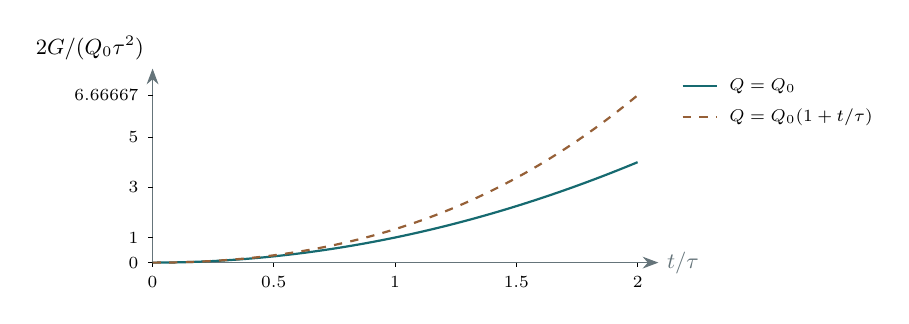
\begin{tikzpicture}[scale=.88,transform shape]
\draw[axis] (0,0.0)--(7.3,0.0) node[right] {$t/\tau$};
\draw[axis] (0,0)--(0,2.8);
\node[above left] at (0,2.8) {$2G/(Q_0\tau^2)$};
\draw[thin] (0.000000,0.0)--(0.000000,-0.06);\node[below,font=\scriptsize] at (0.000000,-0.08) {$ 0 $};
\draw[thin] (1.750000,0.0)--(1.750000,-0.06);\node[below,font=\scriptsize] at (1.750000,-0.08) {$ 0.5 $};
\draw[thin] (3.500000,0.0)--(3.500000,-0.06);\node[below,font=\scriptsize] at (3.500000,-0.08) {$ 1 $};
\draw[thin] (5.250000,0.0)--(5.250000,-0.06);\node[below,font=\scriptsize] at (5.250000,-0.08) {$ 1.5 $};
\draw[thin] (7.000000,0.0)--(7.000000,-0.06);\node[below,font=\scriptsize] at (7.000000,-0.08) {$ 2 $};
\draw[thin] (0,0.000000)--(-.06,0.000000);\node[left,font=\scriptsize] at (-.08,0.000000) {$ 0 $};
\draw[thin] (0,0.362319)--(-.06,0.362319);\node[left,font=\scriptsize] at (-.08,0.362319) {$ 1 $};
\draw[thin] (0,1.086957)--(-.06,1.086957);\node[left,font=\scriptsize] at (-.08,1.086957) {$ 3 $};
\draw[thin] (0,1.811594)--(-.06,1.811594);\node[left,font=\scriptsize] at (-.08,1.811594) {$ 5 $};
\draw[thin] (0,2.415460)--(-.06,2.415460);\node[left,font=\scriptsize] at (-.08,2.415460) {$ 6.66667 $};
\draw[thick,color=accent] plot coordinates {(0.0000000,0.0000000) (0.0291667,0.0000252) (0.0583333,0.0001006) (0.0875000,0.0002264) (0.1166667,0.0004026) (0.1458333,0.0006290) (0.1750000,0.0009058) (0.2041667,0.0012329) (0.2333333,0.0016103) (0.2625000,0.0020380) (0.2916667,0.0025161) (0.3208333,0.0030445) (0.3500000,0.0036232) (0.3791667,0.0042522) (0.4083333,0.0049316) (0.4375000,0.0056612) (0.4666667,0.0064412) (0.4958333,0.0072715) (0.5250000,0.0081522) (0.5541667,0.0090831) (0.5833333,0.0100644) (0.6125000,0.0110960) (0.6416667,0.0121779) (0.6708333,0.0133102) (0.7000000,0.0144928) (0.7291667,0.0157256) (0.7583333,0.0170089) (0.7875000,0.0183424) (0.8166667,0.0197262) (0.8458333,0.0211604) (0.8750000,0.0226449) (0.9041667,0.0241798) (0.9333333,0.0257649) (0.9625000,0.0274004) (0.9916667,0.0290862) (1.0208333,0.0308223) (1.0500000,0.0326087) (1.0791667,0.0344455) (1.1083333,0.0363325) (1.1375000,0.0382699) (1.1666667,0.0402576) (1.1958333,0.0422957) (1.2250000,0.0443841) (1.2541667,0.0465227) (1.2833333,0.0487118) (1.3125000,0.0509511) (1.3416667,0.0532407) (1.3708333,0.0555807) (1.4000000,0.0579710) (1.4291667,0.0604116) (1.4583333,0.0629026) (1.4875000,0.0654438) (1.5166667,0.0680354) (1.5458333,0.0706773) (1.5750000,0.0733696) (1.6041667,0.0761121) (1.6333333,0.0789050) (1.6625000,0.0817482) (1.6916667,0.0846417) (1.7208333,0.0875855) (1.7500000,0.0905797) (1.7791667,0.0936242) (1.8083333,0.0967190) (1.8375000,0.0998641) (1.8666667,0.1030596) (1.8958333,0.1063054) (1.9250000,0.1096014) (1.9541667,0.1129479) (1.9833333,0.1163446) (2.0125000,0.1197917) (2.0416667,0.1232890) (2.0708333,0.1268368) (2.1000000,0.1304348) (2.1291667,0.1340831) (2.1583333,0.1377818) (2.1875000,0.1415308) (2.2166667,0.1453301) (2.2458333,0.1491798) (2.2750000,0.1530797) (2.3041667,0.1570300) (2.3333333,0.1610306) (2.3625000,0.1650815) (2.3916667,0.1691828) (2.4208333,0.1733343) (2.4500000,0.1775362) (2.4791667,0.1817884) (2.5083333,0.1860910) (2.5375000,0.1904438) (2.5666667,0.1948470) (2.5958333,0.1993005) (2.6250000,0.2038043) (2.6541667,0.2083585) (2.6833333,0.2129630) (2.7125000,0.2176178) (2.7416667,0.2223229) (2.7708333,0.2270783) (2.8000000,0.2318841) (2.8291667,0.2367401) (2.8583333,0.2416465) (2.8875000,0.2466033) (2.9166667,0.2516103) (2.9458333,0.2566677) (2.9750000,0.2617754) (3.0041667,0.2669334) (3.0333333,0.2721417) (3.0625000,0.2774004) (3.0916667,0.2827093) (3.1208333,0.2880686) (3.1500000,0.2934783) (3.1791667,0.2989382) (3.2083333,0.3044485) (3.2375000,0.3100091) (3.2666667,0.3156200) (3.2958333,0.3212812) (3.3250000,0.3269928) (3.3541667,0.3327546) (3.3833333,0.3385668) (3.4125000,0.3444293) (3.4416667,0.3503422) (3.4708333,0.3563054) (3.5000000,0.3623188) (3.5291667,0.3683826) (3.5583333,0.3744968) (3.5875000,0.3806612) (3.6166667,0.3868760) (3.6458333,0.3931411) (3.6750000,0.3994565) (3.7041667,0.4058223) (3.7333333,0.4122383) (3.7625000,0.4187047) (3.7916667,0.4252214) (3.8208333,0.4317884) (3.8500000,0.4384058) (3.8791667,0.4450735) (3.9083333,0.4517915) (3.9375000,0.4585598) (3.9666667,0.4653784) (3.9958333,0.4722474) (4.0250000,0.4791667) (4.0541667,0.4861363) (4.0833333,0.4931562) (4.1125000,0.5002264) (4.1416667,0.5073470) (4.1708333,0.5145179) (4.2000000,0.5217391) (4.2291667,0.5290107) (4.2583333,0.5363325) (4.2875000,0.5437047) (4.3166667,0.5511272) (4.3458333,0.5586000) (4.3750000,0.5661232) (4.4041667,0.5736967) (4.4333333,0.5813205) (4.4625000,0.5889946) (4.4916667,0.5967190) (4.5208333,0.6044938) (4.5500000,0.6123188) (4.5791667,0.6201942) (4.6083333,0.6281200) (4.6375000,0.6360960) (4.6666667,0.6441224) (4.6958333,0.6521991) (4.7250000,0.6603261) (4.7541667,0.6685034) (4.7833333,0.6767311) (4.8125000,0.6850091) (4.8416667,0.6933374) (4.8708333,0.7017160) (4.9000000,0.7101449) (4.9291667,0.7186242) (4.9583333,0.7271538) (4.9875000,0.7357337) (5.0166667,0.7443639) (5.0458333,0.7530445) (5.0750000,0.7617754) (5.1041667,0.7705566) (5.1333333,0.7793881) (5.1625000,0.7882699) (5.1916667,0.7972021) (5.2208333,0.8061846) (5.2500000,0.8152174) (5.2791667,0.8243005) (5.3083333,0.8334340) (5.3375000,0.8426178) (5.3666667,0.8518519) (5.3958333,0.8611363) (5.4250000,0.8704710) (5.4541667,0.8798561) (5.4833333,0.8892915) (5.5125000,0.8987772) (5.5416667,0.9083132) (5.5708333,0.9178996) (5.6000000,0.9275362) (5.6291667,0.9372232) (5.6583333,0.9469605) (5.6875000,0.9567482) (5.7166667,0.9665862) (5.7458333,0.9764744) (5.7750000,0.9864130) (5.8041667,0.9964020) (5.8333333,1.0064412) (5.8625000,1.0165308) (5.8916667,1.0266707) (5.9208333,1.0368609) (5.9500000,1.0471014) (5.9791667,1.0573923) (6.0083333,1.0677335) (6.0375000,1.0781250) (6.0666667,1.0885668) (6.0958333,1.0990590) (6.1250000,1.1096014) (6.1541667,1.1201942) (6.1833333,1.1308374) (6.2125000,1.1415308) (6.2416667,1.1522746) (6.2708333,1.1630686) (6.3000000,1.1739130) (6.3291667,1.1848078) (6.3583333,1.1957528) (6.3875000,1.2067482) (6.4166667,1.2177939) (6.4458333,1.2288899) (6.4750000,1.2400362) (6.5041667,1.2512329) (6.5333333,1.2624799) (6.5625000,1.2737772) (6.5916667,1.2851248) (6.6208333,1.2965227) (6.6500000,1.3079710) (6.6791667,1.3194696) (6.7083333,1.3310185) (6.7375000,1.3426178) (6.7666667,1.3542673) (6.7958333,1.3659672) (6.8250000,1.3777174) (6.8541667,1.3895179) (6.8833333,1.4013688) (6.9125000,1.4132699) (6.9416667,1.4252214) (6.9708333,1.4372232) (7.0000000,1.4492754)};
\draw[thick,color=accent] (7.65,2.55)--(8.15,2.55);\node[right,font=\scriptsize] at (8.2,2.55) {$Q=Q_0$};
\draw[thick,dashed,color=warm] plot coordinates {(0.0000000,0.0000000) (0.0291667,0.0000252) (0.0583333,0.0001012) (0.0875000,0.0002283) (0.1166667,0.0004070) (0.1458333,0.0006378) (0.1750000,0.0009209) (0.2041667,0.0012569) (0.2333333,0.0016461) (0.2625000,0.0020890) (0.2916667,0.0025860) (0.3208333,0.0031375) (0.3500000,0.0037440) (0.3791667,0.0044058) (0.4083333,0.0051233) (0.4375000,0.0058971) (0.4666667,0.0067275) (0.4958333,0.0076149) (0.5250000,0.0085598) (0.5541667,0.0095625) (0.5833333,0.0106235) (0.6125000,0.0117433) (0.6416667,0.0129221) (0.6708333,0.0141606) (0.7000000,0.0154589) (0.7291667,0.0168177) (0.7583333,0.0182373) (0.7875000,0.0197181) (0.8166667,0.0212605) (0.8458333,0.0228650) (0.8750000,0.0245320) (0.9041667,0.0262619) (0.9333333,0.0280551) (0.9625000,0.0299121) (0.9916667,0.0318332) (1.0208333,0.0338189) (1.0500000,0.0358696) (1.0791667,0.0379857) (1.1083333,0.0401676) (1.1375000,0.0424158) (1.1666667,0.0447307) (1.1958333,0.0471127) (1.2250000,0.0495622) (1.2541667,0.0520796) (1.2833333,0.0546654) (1.3125000,0.0573200) (1.3416667,0.0600437) (1.3708333,0.0628371) (1.4000000,0.0657005) (1.4291667,0.0686343) (1.4583333,0.0716390) (1.4875000,0.0747151) (1.5166667,0.0778628) (1.5458333,0.0810826) (1.5750000,0.0843750) (1.6041667,0.0877404) (1.6333333,0.0911791) (1.6625000,0.0946917) (1.6916667,0.0982784) (1.7208333,0.1019398) (1.7500000,0.1056763) (1.7791667,0.1094883) (1.8083333,0.1133762) (1.8375000,0.1173404) (1.8666667,0.1213813) (1.8958333,0.1254994) (1.9250000,0.1296950) (1.9541667,0.1339687) (1.9833333,0.1383208) (2.0125000,0.1427517) (2.0416667,0.1472619) (2.0708333,0.1518518) (2.1000000,0.1565217) (2.1291667,0.1612722) (2.1583333,0.1661036) (2.1875000,0.1710164) (2.2166667,0.1760109) (2.2458333,0.1810876) (2.2750000,0.1862470) (2.3041667,0.1914894) (2.3333333,0.1968152) (2.3625000,0.2022249) (2.3916667,0.2077188) (2.4208333,0.2132975) (2.4500000,0.2189614) (2.4791667,0.2247107) (2.5083333,0.2305461) (2.5375000,0.2364678) (2.5666667,0.2424763) (2.5958333,0.2485720) (2.6250000,0.2547554) (2.6541667,0.2610269) (2.6833333,0.2673868) (2.7125000,0.2738357) (2.7416667,0.2803738) (2.7708333,0.2870017) (2.8000000,0.2937198) (2.8291667,0.3005285) (2.8583333,0.3074281) (2.8875000,0.3144192) (2.9166667,0.3215021) (2.9458333,0.3286772) (2.9750000,0.3359450) (3.0041667,0.3433060) (3.0333333,0.3507604) (3.0625000,0.3583088) (3.0916667,0.3659515) (3.1208333,0.3736890) (3.1500000,0.3815217) (3.1791667,0.3894500) (3.2083333,0.3974744) (3.2375000,0.4055952) (3.2666667,0.4138128) (3.2958333,0.4221278) (3.3250000,0.4305405) (3.3541667,0.4390512) (3.3833333,0.4476606) (3.4125000,0.4563689) (3.4416667,0.4651766) (3.4708333,0.4740841) (3.5000000,0.4830918) (3.5291667,0.4922002) (3.5583333,0.5014096) (3.5875000,0.5107205) (3.6166667,0.5201333) (3.6458333,0.5296484) (3.6750000,0.5392663) (3.7041667,0.5489873) (3.7333333,0.5588120) (3.7625000,0.5687406) (3.7916667,0.5787736) (3.8208333,0.5889115) (3.8500000,0.5991546) (3.8791667,0.6095034) (3.9083333,0.6199583) (3.9375000,0.6305197) (3.9666667,0.6411880) (3.9958333,0.6519637) (4.0250000,0.6628472) (4.0541667,0.6738389) (4.0833333,0.6849392) (4.1125000,0.6961485) (4.1416667,0.7074672) (4.1708333,0.7188959) (4.2000000,0.7304348) (4.2291667,0.7420844) (4.2583333,0.7538452) (4.2875000,0.7657175) (4.3166667,0.7777017) (4.3458333,0.7897984) (4.3750000,0.8020079) (4.4041667,0.8143305) (4.4333333,0.8267669) (4.4625000,0.8393173) (4.4916667,0.8519821) (4.5208333,0.8647619) (4.5500000,0.8776570) (4.5791667,0.8906678) (4.6083333,0.9037948) (4.6375000,0.9170384) (4.6666667,0.9303990) (4.6958333,0.9438770) (4.7250000,0.9574728) (4.7541667,0.9711869) (4.7833333,0.9850197) (4.8125000,0.9989715) (4.8416667,1.0130429) (4.8708333,1.0272342) (4.9000000,1.0415459) (4.9291667,1.0559783) (4.9583333,1.0705320) (4.9875000,1.0852072) (5.0166667,1.1000045) (5.0458333,1.1149242) (5.0750000,1.1299668) (5.1041667,1.1451327) (5.1333333,1.1604223) (5.1625000,1.1758360) (5.1916667,1.1913742) (5.2208333,1.2070375) (5.2500000,1.2228261) (5.2791667,1.2387405) (5.3083333,1.2547812) (5.3375000,1.2709484) (5.3666667,1.2872428) (5.3958333,1.3036646) (5.4250000,1.3202144) (5.4541667,1.3368924) (5.4833333,1.3536992) (5.5125000,1.3706352) (5.5416667,1.3877007) (5.5708333,1.4048963) (5.6000000,1.4222222) (5.6291667,1.4396790) (5.6583333,1.4572671) (5.6875000,1.4749868) (5.7166667,1.4928386) (5.7458333,1.5108229) (5.7750000,1.5289402) (5.8041667,1.5471908) (5.8333333,1.5655752) (5.8625000,1.5840938) (5.8916667,1.6027470) (5.9208333,1.6215353) (5.9500000,1.6404589) (5.9791667,1.6595185) (6.0083333,1.6787143) (6.0375000,1.6980469) (6.0666667,1.7175166) (6.0958333,1.7371238) (6.1250000,1.7568690) (6.1541667,1.7767525) (6.1833333,1.7967749) (6.2125000,1.8169365) (6.2416667,1.8372378) (6.2708333,1.8576791) (6.3000000,1.8782609) (6.3291667,1.8989836) (6.3583333,1.9198476) (6.3875000,1.9408533) (6.4166667,1.9620013) (6.4458333,1.9832917) (6.4750000,2.0047252) (6.5041667,2.0263022) (6.5333333,2.0480229) (6.5625000,2.0698879) (6.5916667,2.0918976) (6.6208333,2.1140524) (6.6500000,2.1363527) (6.6791667,2.1587989) (6.7083333,2.1813915) (6.7375000,2.2041308) (6.7666667,2.2270174) (6.7958333,2.2500515) (6.8250000,2.2732337) (6.8541667,2.2965643) (6.8833333,2.3200438) (6.9125000,2.3436726) (6.9416667,2.3674511) (6.9708333,2.3913798) (7.0000000,2.4154589)};
\draw[thick,dashed,color=warm] (7.65,2.0999999999999996)--(8.15,2.0999999999999996);\node[right,font=\scriptsize] at (8.2,2.0999999999999996) {$Q=Q_0(1+t/\tau)$};
\end{tikzpicture}
\figcaption{变图近1.3V5\quad 共同的功率时间积分同时控制平移和转角}
\end{minipage}\end{center}
\item \textbf{另有轴向轨道角动量的光束。}设近轴光束每光子还携带关于$x$轴的轨道角动量$\ell\hbar$，自旋为$\sigma\hbar$，$\sigma=\pm1$，球吸收这两份角动量。求螺距。

纵向线动量按近轴近似取$h/\lambda$，轴向角动量输入率为$(\ell+\sigma)Q/\omega$。故非零$\ell+\sigma$时
\[
 H_{\ell,\sigma}=\frac{H}{|\ell+\sigma|}.
\]
若$\ell=1$，同号自旋给$H/2$，反号自旋使总轴向角动量输入为零，当前确定性转动消失。变图近1.3V6画$\sigma=1$、$\ell=0,1,2,3$的比值。轨道角动量在本变式中由条件直接给定，主解均匀平行光的轨道项按对径对称相消。
\begin{center}\begin{minipage}{.98\linewidth}\centering
\begin{tikzpicture}[scale=.88,transform shape]
\draw[axis] (0,0.0)--(7.3,0.0) node[right] {$\ell\quad(\sigma=1)$};
\draw[axis] (0,0)--(0,2.8);
\node[above left] at (0,2.8) {$H_{\ell,1}/H$};
\draw[thin] (0.000000,0.0)--(0.000000,-0.06);\node[below,font=\scriptsize] at (0.000000,-0.08) {$ 0 $};
\draw[thin] (2.333333,0.0)--(2.333333,-0.06);\node[below,font=\scriptsize] at (2.333333,-0.08) {$ 1 $};
\draw[thin] (4.666667,0.0)--(4.666667,-0.06);\node[below,font=\scriptsize] at (4.666667,-0.08) {$ 2 $};
\draw[thin] (7.000000,0.0)--(7.000000,-0.06);\node[below,font=\scriptsize] at (7.000000,-0.08) {$ 3 $};
\draw[thin] (0,0.000000)--(-.06,0.000000);\node[left,font=\scriptsize] at (-.08,0.000000) {$ 0 $};
\draw[thin] (0,0.595238)--(-.06,0.595238);\node[left,font=\scriptsize] at (-.08,0.595238) {$ 0.25 $};
\draw[thin] (0,1.190476)--(-.06,1.190476);\node[left,font=\scriptsize] at (-.08,1.190476) {$ 0.5 $};
\draw[thin] (0,2.380952)--(-.06,2.380952);\node[left,font=\scriptsize] at (-.08,2.380952) {$ 1 $};
\draw[color=accent] (0.0000000,0.0000000)--(0.0000000,2.3809524);\fill[color=accent] (0.0000000,2.3809524) circle(.04);
\draw[color=accent] (2.3333333,0.0000000)--(2.3333333,1.1904762);\fill[color=accent] (2.3333333,1.1904762) circle(.04);
\draw[color=accent] (4.6666667,0.0000000)--(4.6666667,0.7936508);\fill[color=accent] (4.6666667,0.7936508) circle(.04);
\draw[color=accent] (7.0000000,0.0000000)--(7.0000000,0.5952381);\fill[color=accent] (7.0000000,0.5952381) circle(.04);
\end{tikzpicture}
\figcaption{变图近1.3V6\quad 附加同号轴向轨道角动量提高转动输入}
\end{minipage}\end{center}
\item \textbf{有限光子数的自旋统计。}在一次短时间窗内吸收了固定$N$个光子，各自自旋独立取$\pm\hbar$，均值为$s\hbar$。求输入角动量的均值、方差，并与线动量比较。

单光子自旋二阶矩为$\hbar^2$，方差为$\hbar^2(1-s^2)$。独立相加得
\[
 \langle L_x\rangle=Ns\hbar,\qquad
 \operatorname{Var}(L_x)=N\hbar^2(1-s^2),
 \qquad P_x=Nh/\lambda.
\]
变图近1.3V7取$s=0.6$，画平均自旋$0.6N\hbar$和标准差$0.8\sqrt N\,\hbar$。即使$s=0$，有限光子数仍有$\sqrt N\,\hbar$的统计标准差；主解的同旋圆偏振$s=\pm1$使这一自旋分配方差为零。
\begin{center}\begin{minipage}{.98\linewidth}\centering
\begin{tikzpicture}[scale=.88,transform shape]
\draw[axis] (0,0.0)--(7.3,0.0) node[right] {$N$};
\draw[axis] (0,0)--(0,2.8);
\node[above left] at (0,2.8) {角动量/$\hbar$};
\draw[thin] (0.000000,0.0)--(0.000000,-0.06);\node[below,font=\scriptsize] at (0.000000,-0.08) {$ 0 $};
\draw[thin] (1.750000,0.0)--(1.750000,-0.06);\node[below,font=\scriptsize] at (1.750000,-0.08) {$ 25 $};
\draw[thin] (3.500000,0.0)--(3.500000,-0.06);\node[below,font=\scriptsize] at (3.500000,-0.08) {$ 50 $};
\draw[thin] (5.250000,0.0)--(5.250000,-0.06);\node[below,font=\scriptsize] at (5.250000,-0.08) {$ 75 $};
\draw[thin] (7.000000,0.0)--(7.000000,-0.06);\node[below,font=\scriptsize] at (7.000000,-0.08) {$ 100 $};
\draw[thin] (0,0.000000)--(-.06,0.000000);\node[left,font=\scriptsize] at (-.08,0.000000) {$ 0 $};
\draw[thin] (0,0.384615)--(-.06,0.384615);\node[left,font=\scriptsize] at (-.08,0.384615) {$ 10 $};
\draw[thin] (0,1.153846)--(-.06,1.153846);\node[left,font=\scriptsize] at (-.08,1.153846) {$ 30 $};
\draw[thin] (0,2.307692)--(-.06,2.307692);\node[left,font=\scriptsize] at (-.08,2.307692) {$ 60 $};
\draw[thick,color=accent] plot coordinates {(0.0000000,0.0000000) (0.0291667,0.0096154) (0.0583333,0.0192308) (0.0875000,0.0288462) (0.1166667,0.0384615) (0.1458333,0.0480769) (0.1750000,0.0576923) (0.2041667,0.0673077) (0.2333333,0.0769231) (0.2625000,0.0865385) (0.2916667,0.0961538) (0.3208333,0.1057692) (0.3500000,0.1153846) (0.3791667,0.1250000) (0.4083333,0.1346154) (0.4375000,0.1442308) (0.4666667,0.1538462) (0.4958333,0.1634615) (0.5250000,0.1730769) (0.5541667,0.1826923) (0.5833333,0.1923077) (0.6125000,0.2019231) (0.6416667,0.2115385) (0.6708333,0.2211538) (0.7000000,0.2307692) (0.7291667,0.2403846) (0.7583333,0.2500000) (0.7875000,0.2596154) (0.8166667,0.2692308) (0.8458333,0.2788462) (0.8750000,0.2884615) (0.9041667,0.2980769) (0.9333333,0.3076923) (0.9625000,0.3173077) (0.9916667,0.3269231) (1.0208333,0.3365385) (1.0500000,0.3461538) (1.0791667,0.3557692) (1.1083333,0.3653846) (1.1375000,0.3750000) (1.1666667,0.3846154) (1.1958333,0.3942308) (1.2250000,0.4038462) (1.2541667,0.4134615) (1.2833333,0.4230769) (1.3125000,0.4326923) (1.3416667,0.4423077) (1.3708333,0.4519231) (1.4000000,0.4615385) (1.4291667,0.4711538) (1.4583333,0.4807692) (1.4875000,0.4903846) (1.5166667,0.5000000) (1.5458333,0.5096154) (1.5750000,0.5192308) (1.6041667,0.5288462) (1.6333333,0.5384615) (1.6625000,0.5480769) (1.6916667,0.5576923) (1.7208333,0.5673077) (1.7500000,0.5769231) (1.7791667,0.5865385) (1.8083333,0.5961538) (1.8375000,0.6057692) (1.8666667,0.6153846) (1.8958333,0.6250000) (1.9250000,0.6346154) (1.9541667,0.6442308) (1.9833333,0.6538462) (2.0125000,0.6634615) (2.0416667,0.6730769) (2.0708333,0.6826923) (2.1000000,0.6923077) (2.1291667,0.7019231) (2.1583333,0.7115385) (2.1875000,0.7211538) (2.2166667,0.7307692) (2.2458333,0.7403846) (2.2750000,0.7500000) (2.3041667,0.7596154) (2.3333333,0.7692308) (2.3625000,0.7788462) (2.3916667,0.7884615) (2.4208333,0.7980769) (2.4500000,0.8076923) (2.4791667,0.8173077) (2.5083333,0.8269231) (2.5375000,0.8365385) (2.5666667,0.8461538) (2.5958333,0.8557692) (2.6250000,0.8653846) (2.6541667,0.8750000) (2.6833333,0.8846154) (2.7125000,0.8942308) (2.7416667,0.9038462) (2.7708333,0.9134615) (2.8000000,0.9230769) (2.8291667,0.9326923) (2.8583333,0.9423077) (2.8875000,0.9519231) (2.9166667,0.9615385) (2.9458333,0.9711538) (2.9750000,0.9807692) (3.0041667,0.9903846) (3.0333333,1.0000000) (3.0625000,1.0096154) (3.0916667,1.0192308) (3.1208333,1.0288462) (3.1500000,1.0384615) (3.1791667,1.0480769) (3.2083333,1.0576923) (3.2375000,1.0673077) (3.2666667,1.0769231) (3.2958333,1.0865385) (3.3250000,1.0961538) (3.3541667,1.1057692) (3.3833333,1.1153846) (3.4125000,1.1250000) (3.4416667,1.1346154) (3.4708333,1.1442308) (3.5000000,1.1538462) (3.5291667,1.1634615) (3.5583333,1.1730769) (3.5875000,1.1826923) (3.6166667,1.1923077) (3.6458333,1.2019231) (3.6750000,1.2115385) (3.7041667,1.2211538) (3.7333333,1.2307692) (3.7625000,1.2403846) (3.7916667,1.2500000) (3.8208333,1.2596154) (3.8500000,1.2692308) (3.8791667,1.2788462) (3.9083333,1.2884615) (3.9375000,1.2980769) (3.9666667,1.3076923) (3.9958333,1.3173077) (4.0250000,1.3269231) (4.0541667,1.3365385) (4.0833333,1.3461538) (4.1125000,1.3557692) (4.1416667,1.3653846) (4.1708333,1.3750000) (4.2000000,1.3846154) (4.2291667,1.3942308) (4.2583333,1.4038462) (4.2875000,1.4134615) (4.3166667,1.4230769) (4.3458333,1.4326923) (4.3750000,1.4423077) (4.4041667,1.4519231) (4.4333333,1.4615385) (4.4625000,1.4711538) (4.4916667,1.4807692) (4.5208333,1.4903846) (4.5500000,1.5000000) (4.5791667,1.5096154) (4.6083333,1.5192308) (4.6375000,1.5288462) (4.6666667,1.5384615) (4.6958333,1.5480769) (4.7250000,1.5576923) (4.7541667,1.5673077) (4.7833333,1.5769231) (4.8125000,1.5865385) (4.8416667,1.5961538) (4.8708333,1.6057692) (4.9000000,1.6153846) (4.9291667,1.6250000) (4.9583333,1.6346154) (4.9875000,1.6442308) (5.0166667,1.6538462) (5.0458333,1.6634615) (5.0750000,1.6730769) (5.1041667,1.6826923) (5.1333333,1.6923077) (5.1625000,1.7019231) (5.1916667,1.7115385) (5.2208333,1.7211538) (5.2500000,1.7307692) (5.2791667,1.7403846) (5.3083333,1.7500000) (5.3375000,1.7596154) (5.3666667,1.7692308) (5.3958333,1.7788462) (5.4250000,1.7884615) (5.4541667,1.7980769) (5.4833333,1.8076923) (5.5125000,1.8173077) (5.5416667,1.8269231) (5.5708333,1.8365385) (5.6000000,1.8461538) (5.6291667,1.8557692) (5.6583333,1.8653846) (5.6875000,1.8750000) (5.7166667,1.8846154) (5.7458333,1.8942308) (5.7750000,1.9038462) (5.8041667,1.9134615) (5.8333333,1.9230769) (5.8625000,1.9326923) (5.8916667,1.9423077) (5.9208333,1.9519231) (5.9500000,1.9615385) (5.9791667,1.9711538) (6.0083333,1.9807692) (6.0375000,1.9903846) (6.0666667,2.0000000) (6.0958333,2.0096154) (6.1250000,2.0192308) (6.1541667,2.0288462) (6.1833333,2.0384615) (6.2125000,2.0480769) (6.2416667,2.0576923) (6.2708333,2.0673077) (6.3000000,2.0769231) (6.3291667,2.0865385) (6.3583333,2.0961538) (6.3875000,2.1057692) (6.4166667,2.1153846) (6.4458333,2.1250000) (6.4750000,2.1346154) (6.5041667,2.1442308) (6.5333333,2.1538462) (6.5625000,2.1634615) (6.5916667,2.1730769) (6.6208333,2.1826923) (6.6500000,2.1923077) (6.6791667,2.2019231) (6.7083333,2.2115385) (6.7375000,2.2211538) (6.7666667,2.2307692) (6.7958333,2.2403846) (6.8250000,2.2500000) (6.8541667,2.2596154) (6.8833333,2.2692308) (6.9125000,2.2788462) (6.9416667,2.2884615) (6.9708333,2.2980769) (7.0000000,2.3076923)};
\draw[thick,color=accent] (7.65,2.55)--(8.15,2.55);\node[right,font=\scriptsize] at (8.2,2.55) {$\langle L_x\rangle/\hbar$};
\draw[thick,dashed,color=warm] plot coordinates {(0.0000000,0.0000000) (0.0291667,0.0198615) (0.0583333,0.0280883) (0.0875000,0.0344010) (0.1166667,0.0397229) (0.1458333,0.0444116) (0.1750000,0.0486504) (0.2041667,0.0525485) (0.2333333,0.0561767) (0.2625000,0.0595844) (0.2916667,0.0628074) (0.3208333,0.0658730) (0.3500000,0.0688021) (0.3791667,0.0716115) (0.4083333,0.0743148) (0.4375000,0.0769231) (0.4666667,0.0794458) (0.4958333,0.0818909) (0.5250000,0.0842650) (0.5541667,0.0865741) (0.5833333,0.0888231) (0.6125000,0.0910166) (0.6416667,0.0931585) (0.6708333,0.0952522) (0.7000000,0.0973009) (0.7291667,0.0993073) (0.7583333,0.1012739) (0.7875000,0.1032031) (0.8166667,0.1050969) (0.8458333,0.1069572) (0.8750000,0.1087857) (0.9041667,0.1105839) (0.9333333,0.1123533) (0.9625000,0.1140954) (0.9916667,0.1158112) (1.0208333,0.1175019) (1.0500000,0.1191687) (1.0791667,0.1208125) (1.1083333,0.1224342) (1.1375000,0.1240347) (1.1666667,0.1256149) (1.1958333,0.1271754) (1.2250000,0.1287169) (1.2541667,0.1302403) (1.2833333,0.1317460) (1.3125000,0.1332347) (1.3416667,0.1347069) (1.3708333,0.1361633) (1.4000000,0.1376042) (1.4291667,0.1390302) (1.4583333,0.1404417) (1.4875000,0.1418391) (1.5166667,0.1432230) (1.5458333,0.1445936) (1.5750000,0.1459513) (1.6041667,0.1472965) (1.6333333,0.1486295) (1.6625000,0.1499507) (1.6916667,0.1512603) (1.7208333,0.1525587) (1.7500000,0.1538462) (1.7791667,0.1551229) (1.8083333,0.1563892) (1.8375000,0.1576454) (1.8666667,0.1588916) (1.8958333,0.1601282) (1.9250000,0.1613552) (1.9541667,0.1625730) (1.9833333,0.1637817) (2.0125000,0.1649816) (2.0416667,0.1661728) (2.0708333,0.1673556) (2.1000000,0.1685300) (2.1291667,0.1696963) (2.1583333,0.1708547) (2.1875000,0.1720052) (2.2166667,0.1731481) (2.2458333,0.1742835) (2.2750000,0.1754116) (2.3041667,0.1765325) (2.3333333,0.1776462) (2.3625000,0.1787531) (2.3916667,0.1798531) (2.4208333,0.1809464) (2.4500000,0.1820332) (2.4791667,0.1831135) (2.5083333,0.1841875) (2.5375000,0.1852553) (2.5666667,0.1863169) (2.5958333,0.1873726) (2.6250000,0.1884223) (2.6541667,0.1894662) (2.6833333,0.1905044) (2.7125000,0.1915369) (2.7416667,0.1925639) (2.7708333,0.1935855) (2.8000000,0.1946017) (2.8291667,0.1956126) (2.8583333,0.1966184) (2.8875000,0.1976190) (2.9166667,0.1986145) (2.9458333,0.1996051) (2.9750000,0.2005908) (3.0041667,0.2015717) (3.0333333,0.2025479) (3.0625000,0.2035193) (3.0916667,0.2044862) (3.1208333,0.2054485) (3.1500000,0.2064063) (3.1791667,0.2073597) (3.2083333,0.2083087) (3.2375000,0.2092534) (3.2666667,0.2101939) (3.2958333,0.2111301) (3.3250000,0.2120623) (3.3541667,0.2129904) (3.3833333,0.2139144) (3.4125000,0.2148345) (3.4416667,0.2157506) (3.4708333,0.2166629) (3.5000000,0.2175713) (3.5291667,0.2184760) (3.5583333,0.2193769) (3.5875000,0.2202742) (3.6166667,0.2211678) (3.6458333,0.2220578) (3.6750000,0.2229443) (3.7041667,0.2238272) (3.7333333,0.2247067) (3.7625000,0.2255827) (3.7916667,0.2264554) (3.8208333,0.2273247) (3.8500000,0.2281907) (3.8791667,0.2290535) (3.9083333,0.2299129) (3.9375000,0.2307692) (3.9666667,0.2316224) (3.9958333,0.2324723) (4.0250000,0.2333192) (4.0541667,0.2341631) (4.0833333,0.2350039) (4.1125000,0.2358417) (4.1416667,0.2366765) (4.1708333,0.2375084) (4.2000000,0.2383374) (4.2291667,0.2391636) (4.2583333,0.2399869) (4.2875000,0.2408073) (4.3166667,0.2416250) (4.3458333,0.2424399) (4.3750000,0.2432521) (4.4041667,0.2440616) (4.4333333,0.2448684) (4.4625000,0.2456726) (4.4916667,0.2464742) (4.5208333,0.2472731) (4.5500000,0.2480695) (4.5791667,0.2488633) (4.6083333,0.2496546) (4.6375000,0.2504434) (4.6666667,0.2512297) (4.6958333,0.2520136) (4.7250000,0.2527950) (4.7541667,0.2535741) (4.7833333,0.2543507) (4.8125000,0.2551250) (4.8416667,0.2558969) (4.8708333,0.2566665) (4.9000000,0.2574339) (4.9291667,0.2581989) (4.9583333,0.2589617) (4.9875000,0.2597222) (5.0166667,0.2604805) (5.0458333,0.2612366) (5.0750000,0.2619906) (5.1041667,0.2627423) (5.1333333,0.2634920) (5.1625000,0.2642394) (5.1916667,0.2649848) (5.2208333,0.2657281) (5.2500000,0.2664694) (5.2791667,0.2672085) (5.3083333,0.2679457) (5.3375000,0.2686808) (5.3666667,0.2694139) (5.3958333,0.2701450) (5.4250000,0.2708741) (5.4541667,0.2716013) (5.4833333,0.2723265) (5.5125000,0.2730498) (5.5416667,0.2737712) (5.5708333,0.2744907) (5.6000000,0.2752084) (5.6291667,0.2759241) (5.6583333,0.2766380) (5.6875000,0.2773501) (5.7166667,0.2780603) (5.7458333,0.2787688) (5.7750000,0.2794754) (5.8041667,0.2801803) (5.8333333,0.2808834) (5.8625000,0.2815847) (5.8916667,0.2822843) (5.9208333,0.2829821) (5.9500000,0.2836783) (5.9791667,0.2843727) (6.0083333,0.2850655) (6.0375000,0.2857565) (6.0666667,0.2864459) (6.0958333,0.2871337) (6.1250000,0.2878198) (6.1541667,0.2885043) (6.1833333,0.2891871) (6.2125000,0.2898684) (6.2416667,0.2905480) (6.2708333,0.2912261) (6.3000000,0.2919026) (6.3291667,0.2925775) (6.3583333,0.2932508) (6.3875000,0.2939227) (6.4166667,0.2945930) (6.4458333,0.2952617) (6.4750000,0.2959290) (6.5041667,0.2965947) (6.5333333,0.2972590) (6.5625000,0.2979218) (6.5916667,0.2985831) (6.6208333,0.2992430) (6.6500000,0.2999014) (6.6791667,0.3005583) (6.7083333,0.3012138) (6.7375000,0.3018680) (6.7666667,0.3025206) (6.7958333,0.3031719) (6.8250000,0.3038218) (6.8541667,0.3044703) (6.8833333,0.3051174) (6.9125000,0.3057632) (6.9416667,0.3064076) (6.9708333,0.3070506) (7.0000000,0.3076923)};
\draw[thick,dashed,color=warm] (7.65,2.0999999999999996)--(8.15,2.0999999999999996);\node[right,font=\scriptsize] at (8.2,2.0999999999999996) {$\sigma_L/\hbar$};
\end{tikzpicture}
\figcaption{变图近1.3V7\quad $s=0.6$时平均角动量正比于$N$，标准差正比于$\sqrt N$}
\end{minipage}\end{center}
\item \textbf{螺线的长度与倾角。}某点距轴$b$，螺距为$H$，求转一周的轨迹长度及切线与轴的夹角，并取$b=r$。

以转角$\phi$为参数，轴向导数为$H/(2\pi)$，横向导数长度为$b$。因此每周弧长与倾角为
\[
 L_{\rm turn}=\sqrt{H^2+(2\pi b)^2},\qquad
 \tan\eta=\frac{2\pi b}{H}.
\]
变图近1.3V8画$b/r$对应的$\eta$；$b=r=1\,\mathrm{mm}$、$H=1.5791367\,\mathrm m$时，$\eta$约为$0.228^\circ$。不同点的轨迹半径和每周弧长不同，沿轴的每周增量仍同为$H$。
\begin{center}\begin{minipage}{.98\linewidth}\centering
\begin{tikzpicture}[scale=.88,transform shape]
\draw[axis] (0,0.0)--(7.3,0.0) node[right] {$b/r$};
\draw[axis] (0,0)--(0,2.8);
\node[above left] at (0,2.8) {$\eta/{}^\circ$};
\draw[thin] (0.000000,0.0)--(0.000000,-0.06);\node[below,font=\scriptsize] at (0.000000,-0.08) {$ 0 $};
\draw[thin] (1.750000,0.0)--(1.750000,-0.06);\node[below,font=\scriptsize] at (1.750000,-0.08) {$ 0.25 $};
\draw[thin] (3.500000,0.0)--(3.500000,-0.06);\node[below,font=\scriptsize] at (3.500000,-0.08) {$ 0.5 $};
\draw[thin] (5.250000,0.0)--(5.250000,-0.06);\node[below,font=\scriptsize] at (5.250000,-0.08) {$ 0.75 $};
\draw[thin] (7.000000,0.0)--(7.000000,-0.06);\node[below,font=\scriptsize] at (7.000000,-0.08) {$ 1 $};
\draw[thin] (0,0.000000)--(-.06,0.000000);\node[left,font=\scriptsize] at (-.08,0.000000) {$ 0 $};
\draw[thin] (0,1.041667)--(-.06,1.041667);\node[left,font=\scriptsize] at (-.08,1.041667) {$ 0.1 $};
\draw[thin] (0,2.083333)--(-.06,2.083333);\node[left,font=\scriptsize] at (-.08,2.083333) {$ 0.2 $};
\draw[thick,color=accent] plot coordinates {(0.0000000,0.0000000) (0.0291667,0.0098946) (0.0583333,0.0197893) (0.0875000,0.0296839) (0.1166667,0.0395786) (0.1458333,0.0494732) (0.1750000,0.0593679) (0.2041667,0.0692625) (0.2333333,0.0791572) (0.2625000,0.0890518) (0.2916667,0.0989465) (0.3208333,0.1088411) (0.3500000,0.1187358) (0.3791667,0.1286304) (0.4083333,0.1385251) (0.4375000,0.1484197) (0.4666667,0.1583143) (0.4958333,0.1682090) (0.5250000,0.1781036) (0.5541667,0.1879983) (0.5833333,0.1978929) (0.6125000,0.2077876) (0.6416667,0.2176822) (0.6708333,0.2275769) (0.7000000,0.2374715) (0.7291667,0.2473662) (0.7583333,0.2572608) (0.7875000,0.2671554) (0.8166667,0.2770501) (0.8458333,0.2869447) (0.8750000,0.2968394) (0.9041667,0.3067340) (0.9333333,0.3166287) (0.9625000,0.3265233) (0.9916667,0.3364180) (1.0208333,0.3463126) (1.0500000,0.3562072) (1.0791667,0.3661019) (1.1083333,0.3759965) (1.1375000,0.3858912) (1.1666667,0.3957858) (1.1958333,0.4056805) (1.2250000,0.4155751) (1.2541667,0.4254697) (1.2833333,0.4353644) (1.3125000,0.4452590) (1.3416667,0.4551537) (1.3708333,0.4650483) (1.4000000,0.4749429) (1.4291667,0.4848376) (1.4583333,0.4947322) (1.4875000,0.5046269) (1.5166667,0.5145215) (1.5458333,0.5244161) (1.5750000,0.5343108) (1.6041667,0.5442054) (1.6333333,0.5541001) (1.6625000,0.5639947) (1.6916667,0.5738893) (1.7208333,0.5837840) (1.7500000,0.5936786) (1.7791667,0.6035733) (1.8083333,0.6134679) (1.8375000,0.6233625) (1.8666667,0.6332572) (1.8958333,0.6431518) (1.9250000,0.6530464) (1.9541667,0.6629411) (1.9833333,0.6728357) (2.0125000,0.6827303) (2.0416667,0.6926250) (2.0708333,0.7025196) (2.1000000,0.7124142) (2.1291667,0.7223089) (2.1583333,0.7322035) (2.1875000,0.7420981) (2.2166667,0.7519928) (2.2458333,0.7618874) (2.2750000,0.7717820) (2.3041667,0.7816767) (2.3333333,0.7915713) (2.3625000,0.8014659) (2.3916667,0.8113605) (2.4208333,0.8212552) (2.4500000,0.8311498) (2.4791667,0.8410444) (2.5083333,0.8509391) (2.5375000,0.8608337) (2.5666667,0.8707283) (2.5958333,0.8806229) (2.6250000,0.8905176) (2.6541667,0.9004122) (2.6833333,0.9103068) (2.7125000,0.9202014) (2.7416667,0.9300961) (2.7708333,0.9399907) (2.8000000,0.9498853) (2.8291667,0.9597799) (2.8583333,0.9696745) (2.8875000,0.9795692) (2.9166667,0.9894638) (2.9458333,0.9993584) (2.9750000,1.0092530) (3.0041667,1.0191476) (3.0333333,1.0290423) (3.0625000,1.0389369) (3.0916667,1.0488315) (3.1208333,1.0587261) (3.1500000,1.0686207) (3.1791667,1.0785153) (3.2083333,1.0884099) (3.2375000,1.0983046) (3.2666667,1.1081992) (3.2958333,1.1180938) (3.3250000,1.1279884) (3.3541667,1.1378830) (3.3833333,1.1477776) (3.4125000,1.1576722) (3.4416667,1.1675668) (3.4708333,1.1774614) (3.5000000,1.1873561) (3.5291667,1.1972507) (3.5583333,1.2071453) (3.5875000,1.2170399) (3.6166667,1.2269345) (3.6458333,1.2368291) (3.6750000,1.2467237) (3.7041667,1.2566183) (3.7333333,1.2665129) (3.7625000,1.2764075) (3.7916667,1.2863021) (3.8208333,1.2961967) (3.8500000,1.3060913) (3.8791667,1.3159859) (3.9083333,1.3258805) (3.9375000,1.3357751) (3.9666667,1.3456697) (3.9958333,1.3555643) (4.0250000,1.3654589) (4.0541667,1.3753535) (4.0833333,1.3852481) (4.1125000,1.3951427) (4.1416667,1.4050373) (4.1708333,1.4149318) (4.2000000,1.4248264) (4.2291667,1.4347210) (4.2583333,1.4446156) (4.2875000,1.4545102) (4.3166667,1.4644048) (4.3458333,1.4742994) (4.3750000,1.4841940) (4.4041667,1.4940886) (4.4333333,1.5039831) (4.4625000,1.5138777) (4.4916667,1.5237723) (4.5208333,1.5336669) (4.5500000,1.5435615) (4.5791667,1.5534560) (4.6083333,1.5633506) (4.6375000,1.5732452) (4.6666667,1.5831398) (4.6958333,1.5930344) (4.7250000,1.6029289) (4.7541667,1.6128235) (4.7833333,1.6227181) (4.8125000,1.6326127) (4.8416667,1.6425072) (4.8708333,1.6524018) (4.9000000,1.6622964) (4.9291667,1.6721909) (4.9583333,1.6820855) (4.9875000,1.6919801) (5.0166667,1.7018746) (5.0458333,1.7117692) (5.0750000,1.7216638) (5.1041667,1.7315583) (5.1333333,1.7414529) (5.1625000,1.7513475) (5.1916667,1.7612420) (5.2208333,1.7711366) (5.2500000,1.7810311) (5.2791667,1.7909257) (5.3083333,1.8008203) (5.3375000,1.8107148) (5.3666667,1.8206094) (5.3958333,1.8305039) (5.4250000,1.8403985) (5.4541667,1.8502930) (5.4833333,1.8601876) (5.5125000,1.8700821) (5.5416667,1.8799767) (5.5708333,1.8898712) (5.6000000,1.8997658) (5.6291667,1.9096603) (5.6583333,1.9195549) (5.6875000,1.9294494) (5.7166667,1.9393440) (5.7458333,1.9492385) (5.7750000,1.9591330) (5.8041667,1.9690276) (5.8333333,1.9789221) (5.8625000,1.9888167) (5.8916667,1.9987112) (5.9208333,2.0086057) (5.9500000,2.0185003) (5.9791667,2.0283948) (6.0083333,2.0382893) (6.0375000,2.0481839) (6.0666667,2.0580784) (6.0958333,2.0679729) (6.1250000,2.0778674) (6.1541667,2.0877620) (6.1833333,2.0976565) (6.2125000,2.1075510) (6.2416667,2.1174455) (6.2708333,2.1273401) (6.3000000,2.1372346) (6.3291667,2.1471291) (6.3583333,2.1570236) (6.3875000,2.1669181) (6.4166667,2.1768127) (6.4458333,2.1867072) (6.4750000,2.1966017) (6.5041667,2.2064962) (6.5333333,2.2163907) (6.5625000,2.2262852) (6.5916667,2.2361797) (6.6208333,2.2460742) (6.6500000,2.2559687) (6.6791667,2.2658632) (6.7083333,2.2757577) (6.7375000,2.2856522) (6.7666667,2.2955467) (6.7958333,2.3054412) (6.8250000,2.3153357) (6.8541667,2.3252302) (6.8833333,2.3351247) (6.9125000,2.3450192) (6.9416667,2.3549137) (6.9708333,2.3648082) (7.0000000,2.3747027)};
\end{tikzpicture}
\figcaption{变图近1.3V8\quad 物质点离轴距离改变轨迹倾角，每周轴向位移仍为$H$}
\end{minipage}\end{center}
\end{enumerate}

\Needspace{13\baselineskip}

\pdfbookmark[2]{第 4 题 多层黑板间的辐射传热}{q4}

\section*{第 4 题\quad 多层黑板间的辐射传热}\label{q:4}

两块足够大的平行黑色平板温度分别维持100°C和10°C，板间为真空。中间再放入两块同样大小的平行黑板，各板温度均匀，中间两板不连接外部热源，忽略边缘效应及其他热交换。求中间两板的平衡温度，以及净传热能流密度与未插板时的比。

\begin{center}\begin{minipage}{.98\linewidth}\centering
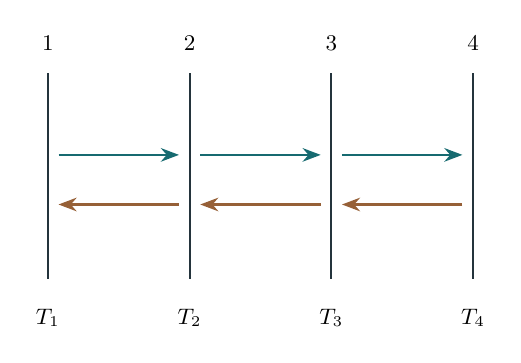
\begin{tikzpicture}[scale=.9,transform shape]
\draw[object] (0.00000,-1.30000)--(0.00000,1.60000);\node[above] at (0.00000,1.80000) {1};\node[below] at (0.00000,-1.60000) {$T_1$};\draw[motion] (0.15000,0.45000)--(1.85000,0.45000);\draw[force] (1.85000,-0.25000)--(0.15000,-0.25000);\draw[object] (2.00000,-1.30000)--(2.00000,1.60000);\node[above] at (2.00000,1.80000) {2};\node[below] at (2.00000,-1.60000) {$T_2$};\draw[motion] (2.15000,0.45000)--(3.85000,0.45000);\draw[force] (3.85000,-0.25000)--(2.15000,-0.25000);\draw[object] (4.00000,-1.30000)--(4.00000,1.60000);\node[above] at (4.00000,1.80000) {3};\node[below] at (4.00000,-1.60000) {$T_3$};\draw[motion] (4.15000,0.45000)--(5.85000,0.45000);\draw[force] (5.85000,-0.25000)--(4.15000,-0.25000);\draw[object] (6.00000,-1.30000)--(6.00000,1.60000);\node[above] at (6.00000,1.80000) {4};\node[below] at (6.00000,-1.60000) {$T_4$};
\end{tikzpicture}
\figcaption{图近1.4\quad 各间隙有相向辐射，中间板温度由平衡决定。}
\end{minipage}\end{center}

\Needspace{8\baselineskip}

\pdfbookmark[3]{题型定位}{q4-h0}

\subsection*{题型定位}

中间每板的两面同时吸收和发射，稳态能量守恒使各相邻间隙净流相等。以绝对温度四次方为变量求线性温度分配，再还原内板温度与总传热比。

\Needspace{8\baselineskip}

\pdfbookmark[3]{知识点}{q4-h1}

\subsection*{知识点}

\begin{itemize}
\item 黑表面向半空间的出射度为$\sigma T^4$，净交换为两相对表面的出射度差。
\item 内板左右净流之差改变内能，稳态时三段净流相同。
\item 无限平行面视角因子为1，各板内部导热保证两面等温，内板仅通过相邻表面间的辐射交换改变内能。
\item 等差的是$T^4$，小温差下再将其展开成近似等差的温度。
\end{itemize}

\Needspace{8\baselineskip}

\pdfbookmark[3]{物理图像}{q4-h2}

\subsection*{物理图像}

解图A画四板间三段相同净流，B把一个内板的两份吸收与两份发射分开，C比较四次方变量和温度的排列，D给屏数与传热比。每个表面保持黑体辐射性质，插板改变的是热端到冷端的净交换分配。

\Needspace{8\baselineskip}

\pdfbookmark[3]{解题入口}{q4-h3}

\subsection*{解题入口}

把给定摄氏温度换成K，再给板2和板3各写一个零净吸热方程。设$X=T^4$，把这两式变为二元线性方程，求解后开四次方；最后从同一个等流条件求插板与未插板的比值。

\Needspace{8\baselineskip}

\pdfbookmark[3]{标准解法}{q4-h4}

\subsection*{标准解法}


图近1.4从热端到冷端依次标板1、2、3、4。两端温度由外界维持，中间两板仅靠辐射交换达到稳态。先换成热力学温度，$T_1=373.15\,\mathrm K$、$T_4=283.15\,\mathrm K$，Stefan定律中的温度均用K。

每个黑表面向它面前的半空间发出$\sigma T^4$的能流密度。无限平行面的相互视角因子为1，一面的全部半空间辐射都到达相邻板。虽然单条光线可以斜射，角分布积分后的净能流沿法线。黑板不透光，板两侧分别与各自相邻的表面交换。因此相邻两板间沿热端到冷端的净流为
\[
q_{j,j+1}=\sigma(T_j^4-T_{j+1}^4).
\]
解图近1.4A画三条间隙中的净流；每条净流由相向的两份辐射相减得到。板内部导热使同一板的两面等温，支撑导热、边缘绕行和其他外部热交换按题设忽略。
\begin{center}\begin{minipage}{.98\linewidth}\centering
\begin{tikzpicture}[scale=.9,transform shape]
\draw[object] (0,-1.5)--(0,1.5);\node[above] at (0,1.6) {$T_1$};\node[below] at (0,-1.6) {板1};
\draw[force] (0.3,0)--(1.7,0) node[midway,above] {$q$};
\draw[object] (2,-1.5)--(2,1.5);\node[above] at (2,1.6) {$T_2$};\node[below] at (2,-1.6) {板2};
\draw[force] (2.3,0)--(3.7,0) node[midway,above] {$q$};
\draw[object] (4,-1.5)--(4,1.5);\node[above] at (4,1.6) {$T_3$};\node[below] at (4,-1.6) {板3};
\draw[force] (4.3,0)--(5.7,0) node[midway,above] {$q$};
\draw[object] (6,-1.5)--(6,1.5);\node[above] at (6,1.6) {$T_4$};\node[below] at (6,-1.6) {板4};
\node[left] at (-.5,.8) {热端};\node[right] at (6.5,.8) {冷端};
\end{tikzpicture}
\figcaption{解图近1.4A\quad 四板之间的三段稳态净辐射流相同}
\end{minipage}\end{center}
对中间板2，左面净吸收$\sigma(T_1^4-T_2^4)$，右面净吸收$\sigma(T_3^4-T_2^4)$。两面发射都使用板2的同一温度，稳态的单位面积能量守恒为
\[
 0=\sigma T_1^4+\sigma T_3^4-2\sigma T_2^4.
\]
板3同样吸收板2和板4的辐射，两面各发射$\sigma T_3^4$，所以
\[
T_1^4+T_3^4=2T_2^4,\qquad T_2^4+T_4^4=2T_3^4,
\]
解图近1.4B把一个内板的四项能量画开，两个发射项相加给系数2。若左、右净流暂时不同，其差改变板的内能，直到温度使两者相等。
\begin{center}\begin{minipage}{.98\linewidth}\centering
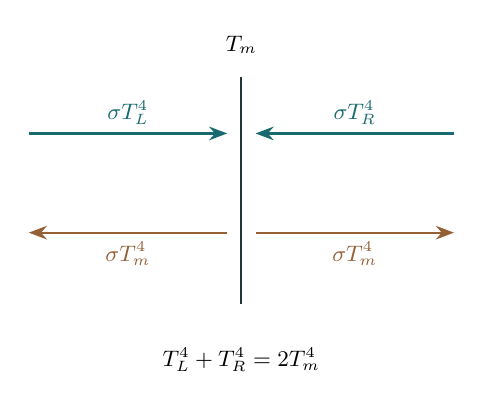
\begin{tikzpicture}[scale=.9,transform shape]
\draw[object] (0,-1.6)--(0,1.6);\node[above] at (0,1.8) {$T_m$};
\draw[motion] (-3,.8)--(-.2,.8) node[midway,above] {$\sigma T_L^4$};
\draw[force,color=warm] (-.2,-.6)--(-3,-.6) node[midway,below] {$\sigma T_m^4$};
\draw[motion] (3,.8)--(.2,.8) node[midway,above] {$\sigma T_R^4$};
\draw[force,color=warm] (.2,-.6)--(3,-.6) node[midway,below] {$\sigma T_m^4$};
\node[below] at (0,-2.1) {$T_L^4+T_R^4=2T_m^4$};
\end{tikzpicture}
\figcaption{解图近1.4B\quad 一个内板的两份吸收与两面发射}
\end{minipage}\end{center}
记$X_j=T_j^4$，上述方程成为$2X_2-X_3=X_1$、$-X_2+2X_3=X_4$。将第一式乘2再与第二式相加，得$3X_2=2X_1+X_4$；把$X_2$代回，得$3X_3=X_1+2X_4$。因此
\[
\boxed{T_2=\left(\frac{2T_1^4+T_4^4}{3}\right)^{1/4}=350.36\,\mathrm K},
\quad
\boxed{T_3=\left(\frac{T_1^4+2T_4^4}{3}\right)^{1/4}=321.98\,\mathrm K}.
\]
换回摄氏温度约为$77.21^\circ\mathrm C$和$48.83^\circ\mathrm C$。解图近1.4C取$T_h=T_1$、$T_c=T_4$，画$X_j$的等差排列，同时显示还原后的温度变化；四次方变量的等差关系直接给
\[
T_1^4-T_2^4=T_2^4-T_3^4=T_3^4-T_4^4
=\frac{T_1^4-T_4^4}{3}.
\]
\begin{center}\begin{minipage}{.98\linewidth}\centering
\begin{tikzpicture}[scale=.88,transform shape]
\draw[axis] (0,0.0)--(7.3,0.0) node[right] {$j$};
\draw[axis] (0,0)--(0,2.8);
\node[above left] at (0,2.8) {归一化量};
\draw[thin] (0.000000,0.0)--(0.000000,-0.06);\node[below,font=\scriptsize] at (0.000000,-0.08) {$ 1 $};
\draw[thin] (2.333333,0.0)--(2.333333,-0.06);\node[below,font=\scriptsize] at (2.333333,-0.08) {$ 2 $};
\draw[thin] (4.666667,0.0)--(4.666667,-0.06);\node[below,font=\scriptsize] at (4.666667,-0.08) {$ 3 $};
\draw[thin] (7.000000,0.0)--(7.000000,-0.06);\node[below,font=\scriptsize] at (7.000000,-0.08) {$ 4 $};
\draw[thin] (0,0.000000)--(-.06,0.000000);\node[left,font=\scriptsize] at (-.08,0.000000) {$ 0 $};
\draw[thin] (0,0.793651)--(-.06,0.793651);\node[left,font=\scriptsize] at (-.08,0.793651) {$ 0.333333 $};
\draw[thin] (0,1.587302)--(-.06,1.587302);\node[left,font=\scriptsize] at (-.08,1.587302) {$ 0.666667 $};
\draw[thin] (0,2.380952)--(-.06,2.380952);\node[left,font=\scriptsize] at (-.08,2.380952) {$ 1 $};
\draw[thick,color=accent] plot coordinates {(0.0000000,2.3809524) (0.0291667,2.3710317) (0.0583333,2.3611111) (0.0875000,2.3511905) (0.1166667,2.3412698) (0.1458333,2.3313492) (0.1750000,2.3214286) (0.2041667,2.3115079) (0.2333333,2.3015873) (0.2625000,2.2916667) (0.2916667,2.2817460) (0.3208333,2.2718254) (0.3500000,2.2619048) (0.3791667,2.2519841) (0.4083333,2.2420635) (0.4375000,2.2321429) (0.4666667,2.2222222) (0.4958333,2.2123016) (0.5250000,2.2023810) (0.5541667,2.1924603) (0.5833333,2.1825397) (0.6125000,2.1726190) (0.6416667,2.1626984) (0.6708333,2.1527778) (0.7000000,2.1428571) (0.7291667,2.1329365) (0.7583333,2.1230159) (0.7875000,2.1130952) (0.8166667,2.1031746) (0.8458333,2.0932540) (0.8750000,2.0833333) (0.9041667,2.0734127) (0.9333333,2.0634921) (0.9625000,2.0535714) (0.9916667,2.0436508) (1.0208333,2.0337302) (1.0500000,2.0238095) (1.0791667,2.0138889) (1.1083333,2.0039683) (1.1375000,1.9940476) (1.1666667,1.9841270) (1.1958333,1.9742063) (1.2250000,1.9642857) (1.2541667,1.9543651) (1.2833333,1.9444444) (1.3125000,1.9345238) (1.3416667,1.9246032) (1.3708333,1.9146825) (1.4000000,1.9047619) (1.4291667,1.8948413) (1.4583333,1.8849206) (1.4875000,1.8750000) (1.5166667,1.8650794) (1.5458333,1.8551587) (1.5750000,1.8452381) (1.6041667,1.8353175) (1.6333333,1.8253968) (1.6625000,1.8154762) (1.6916667,1.8055556) (1.7208333,1.7956349) (1.7500000,1.7857143) (1.7791667,1.7757937) (1.8083333,1.7658730) (1.8375000,1.7559524) (1.8666667,1.7460317) (1.8958333,1.7361111) (1.9250000,1.7261905) (1.9541667,1.7162698) (1.9833333,1.7063492) (2.0125000,1.6964286) (2.0416667,1.6865079) (2.0708333,1.6765873) (2.1000000,1.6666667) (2.1291667,1.6567460) (2.1583333,1.6468254) (2.1875000,1.6369048) (2.2166667,1.6269841) (2.2458333,1.6170635) (2.2750000,1.6071429) (2.3041667,1.5972222) (2.3333333,1.5873016) (2.3625000,1.5773810) (2.3916667,1.5674603) (2.4208333,1.5575397) (2.4500000,1.5476190) (2.4791667,1.5376984) (2.5083333,1.5277778) (2.5375000,1.5178571) (2.5666667,1.5079365) (2.5958333,1.4980159) (2.6250000,1.4880952) (2.6541667,1.4781746) (2.6833333,1.4682540) (2.7125000,1.4583333) (2.7416667,1.4484127) (2.7708333,1.4384921) (2.8000000,1.4285714) (2.8291667,1.4186508) (2.8583333,1.4087302) (2.8875000,1.3988095) (2.9166667,1.3888889) (2.9458333,1.3789683) (2.9750000,1.3690476) (3.0041667,1.3591270) (3.0333333,1.3492063) (3.0625000,1.3392857) (3.0916667,1.3293651) (3.1208333,1.3194444) (3.1500000,1.3095238) (3.1791667,1.2996032) (3.2083333,1.2896825) (3.2375000,1.2797619) (3.2666667,1.2698413) (3.2958333,1.2599206) (3.3250000,1.2500000) (3.3541667,1.2400794) (3.3833333,1.2301587) (3.4125000,1.2202381) (3.4416667,1.2103175) (3.4708333,1.2003968) (3.5000000,1.1904762) (3.5291667,1.1805556) (3.5583333,1.1706349) (3.5875000,1.1607143) (3.6166667,1.1507937) (3.6458333,1.1408730) (3.6750000,1.1309524) (3.7041667,1.1210317) (3.7333333,1.1111111) (3.7625000,1.1011905) (3.7916667,1.0912698) (3.8208333,1.0813492) (3.8500000,1.0714286) (3.8791667,1.0615079) (3.9083333,1.0515873) (3.9375000,1.0416667) (3.9666667,1.0317460) (3.9958333,1.0218254) (4.0250000,1.0119048) (4.0541667,1.0019841) (4.0833333,0.9920635) (4.1125000,0.9821429) (4.1416667,0.9722222) (4.1708333,0.9623016) (4.2000000,0.9523810) (4.2291667,0.9424603) (4.2583333,0.9325397) (4.2875000,0.9226190) (4.3166667,0.9126984) (4.3458333,0.9027778) (4.3750000,0.8928571) (4.4041667,0.8829365) (4.4333333,0.8730159) (4.4625000,0.8630952) (4.4916667,0.8531746) (4.5208333,0.8432540) (4.5500000,0.8333333) (4.5791667,0.8234127) (4.6083333,0.8134921) (4.6375000,0.8035714) (4.6666667,0.7936508) (4.6958333,0.7837302) (4.7250000,0.7738095) (4.7541667,0.7638889) (4.7833333,0.7539683) (4.8125000,0.7440476) (4.8416667,0.7341270) (4.8708333,0.7242063) (4.9000000,0.7142857) (4.9291667,0.7043651) (4.9583333,0.6944444) (4.9875000,0.6845238) (5.0166667,0.6746032) (5.0458333,0.6646825) (5.0750000,0.6547619) (5.1041667,0.6448413) (5.1333333,0.6349206) (5.1625000,0.6250000) (5.1916667,0.6150794) (5.2208333,0.6051587) (5.2500000,0.5952381) (5.2791667,0.5853175) (5.3083333,0.5753968) (5.3375000,0.5654762) (5.3666667,0.5555556) (5.3958333,0.5456349) (5.4250000,0.5357143) (5.4541667,0.5257937) (5.4833333,0.5158730) (5.5125000,0.5059524) (5.5416667,0.4960317) (5.5708333,0.4861111) (5.6000000,0.4761905) (5.6291667,0.4662698) (5.6583333,0.4563492) (5.6875000,0.4464286) (5.7166667,0.4365079) (5.7458333,0.4265873) (5.7750000,0.4166667) (5.8041667,0.4067460) (5.8333333,0.3968254) (5.8625000,0.3869048) (5.8916667,0.3769841) (5.9208333,0.3670635) (5.9500000,0.3571429) (5.9791667,0.3472222) (6.0083333,0.3373016) (6.0375000,0.3273810) (6.0666667,0.3174603) (6.0958333,0.3075397) (6.1250000,0.2976190) (6.1541667,0.2876984) (6.1833333,0.2777778) (6.2125000,0.2678571) (6.2416667,0.2579365) (6.2708333,0.2480159) (6.3000000,0.2380952) (6.3291667,0.2281746) (6.3583333,0.2182540) (6.3875000,0.2083333) (6.4166667,0.1984127) (6.4458333,0.1884921) (6.4750000,0.1785714) (6.5041667,0.1686508) (6.5333333,0.1587302) (6.5625000,0.1488095) (6.5916667,0.1388889) (6.6208333,0.1289683) (6.6500000,0.1190476) (6.6791667,0.1091270) (6.7083333,0.0992063) (6.7375000,0.0892857) (6.7666667,0.0793651) (6.7958333,0.0694444) (6.8250000,0.0595238) (6.8541667,0.0496032) (6.8833333,0.0396825) (6.9125000,0.0297619) (6.9416667,0.0198413) (6.9708333,0.0099206) (7.0000000,0.0000000)};
\draw[thick,color=accent] (7.65,2.55)--(8.15,2.55);\node[right,font=\scriptsize] at (8.2,2.55) {$(T_j^4-T_c^4)/(T_h^4-T_c^4)$};
\draw[thick,dashed,color=warm] plot coordinates {(0.0000000,2.3809524) (0.0291667,2.3740714) (0.0583333,2.3671759) (0.0875000,2.3602660) (0.1166667,2.3533415) (0.1458333,2.3464024) (0.1750000,2.3394485) (0.2041667,2.3324799) (0.2333333,2.3254963) (0.2625000,2.3184979) (0.2916667,2.3114844) (0.3208333,2.3044559) (0.3500000,2.2974122) (0.3791667,2.2903532) (0.4083333,2.2832790) (0.4375000,2.2761893) (0.4666667,2.2690842) (0.4958333,2.2619635) (0.5250000,2.2548272) (0.5541667,2.2476751) (0.5833333,2.2405073) (0.6125000,2.2333236) (0.6416667,2.2261240) (0.6708333,2.2189083) (0.7000000,2.2116765) (0.7291667,2.2044285) (0.7583333,2.1971641) (0.7875000,2.1898835) (0.8166667,2.1825863) (0.8458333,2.1752726) (0.8750000,2.1679423) (0.9041667,2.1605952) (0.9333333,2.1532313) (0.9625000,2.1458505) (0.9916667,2.1384527) (1.0208333,2.1310378) (1.0500000,2.1236057) (1.0791667,2.1161564) (1.1083333,2.1086897) (1.1375000,2.1012055) (1.1666667,2.0937038) (1.1958333,2.0861844) (1.2250000,2.0786472) (1.2541667,2.0710922) (1.2833333,2.0635193) (1.3125000,2.0559283) (1.3416667,2.0483191) (1.3708333,2.0406917) (1.4000000,2.0330460) (1.4291667,2.0253818) (1.4583333,2.0176990) (1.4875000,2.0099975) (1.5166667,2.0022773) (1.5458333,1.9945382) (1.5750000,1.9867801) (1.6041667,1.9790029) (1.6333333,1.9712065) (1.6625000,1.9633908) (1.6916667,1.9555557) (1.7208333,1.9477010) (1.7500000,1.9398266) (1.7791667,1.9319325) (1.8083333,1.9240184) (1.8375000,1.9160844) (1.8666667,1.9081303) (1.8958333,1.9001559) (1.9250000,1.8921611) (1.9541667,1.8841458) (1.9833333,1.8761100) (2.0125000,1.8680533) (2.0416667,1.8599759) (2.0708333,1.8518774) (2.1000000,1.8437579) (2.1291667,1.8356171) (2.1583333,1.8274549) (2.1875000,1.8192712) (2.2166667,1.8110658) (2.2458333,1.8028387) (2.2750000,1.7945897) (2.3041667,1.7863187) (2.3333333,1.7780255) (2.3625000,1.7697099) (2.3916667,1.7613719) (2.4208333,1.7530113) (2.4500000,1.7446279) (2.4791667,1.7362216) (2.5083333,1.7277923) (2.5375000,1.7193399) (2.5666667,1.7108640) (2.5958333,1.7023647) (2.6250000,1.6938418) (2.6541667,1.6852950) (2.6833333,1.6767244) (2.7125000,1.6681296) (2.7416667,1.6595105) (2.7708333,1.6508670) (2.8000000,1.6421989) (2.8291667,1.6335061) (2.8583333,1.6247884) (2.8875000,1.6160456) (2.9166667,1.6072775) (2.9458333,1.5984840) (2.9750000,1.5896649) (3.0041667,1.5808200) (3.0333333,1.5719492) (3.0625000,1.5630523) (3.0916667,1.5541290) (3.1208333,1.5451793) (3.1500000,1.5362029) (3.1791667,1.5271996) (3.2083333,1.5181693) (3.2375000,1.5091117) (3.2666667,1.5000268) (3.2958333,1.4909142) (3.3250000,1.4817737) (3.3541667,1.4726053) (3.3833333,1.4634086) (3.4125000,1.4541835) (3.4416667,1.4449298) (3.4708333,1.4356472) (3.5000000,1.4263356) (3.5291667,1.4169948) (3.5583333,1.4076244) (3.5875000,1.3982244) (3.6166667,1.3887944) (3.6458333,1.3793343) (3.6750000,1.3698438) (3.7041667,1.3603228) (3.7333333,1.3507709) (3.7625000,1.3411879) (3.7916667,1.3315737) (3.8208333,1.3219279) (3.8500000,1.3122504) (3.8791667,1.3025408) (3.9083333,1.2927989) (3.9375000,1.2830246) (3.9666667,1.2732174) (3.9958333,1.2633772) (4.0250000,1.2535038) (4.0541667,1.2435967) (4.0833333,1.2336559) (4.1125000,1.2236809) (4.1416667,1.2136716) (4.1708333,1.2036276) (4.2000000,1.1935487) (4.2291667,1.1834345) (4.2583333,1.1732849) (4.2875000,1.1630995) (4.3166667,1.1528780) (4.3458333,1.1426201) (4.3750000,1.1323255) (4.4041667,1.1219939) (4.4333333,1.1116249) (4.4625000,1.1012184) (4.4916667,1.0907739) (4.5208333,1.0802911) (4.5500000,1.0697697) (4.5791667,1.0592094) (4.6083333,1.0486098) (4.6375000,1.0379706) (4.6666667,1.0272914) (4.6958333,1.0165719) (4.7250000,1.0058117) (4.7541667,0.9950105) (4.7833333,0.9841679) (4.8125000,0.9732835) (4.8416667,0.9623569) (4.8708333,0.9513879) (4.9000000,0.9403759) (4.9291667,0.9293205) (4.9583333,0.9182215) (4.9875000,0.9070783) (5.0166667,0.8958906) (5.0458333,0.8846580) (5.0750000,0.8733799) (5.1041667,0.8620561) (5.1333333,0.8506860) (5.1625000,0.8392692) (5.1916667,0.8278053) (5.2208333,0.8162938) (5.2500000,0.8047343) (5.2791667,0.7931262) (5.3083333,0.7814691) (5.3375000,0.7697625) (5.3666667,0.7580060) (5.3958333,0.7461989) (5.4250000,0.7343409) (5.4541667,0.7224314) (5.4833333,0.7104698) (5.5125000,0.6984556) (5.5416667,0.6863884) (5.5708333,0.6742674) (5.6000000,0.6620923) (5.6291667,0.6498624) (5.6583333,0.6375771) (5.6875000,0.6252358) (5.7166667,0.6128380) (5.7458333,0.6003830) (5.7750000,0.5878702) (5.8041667,0.5752990) (5.8333333,0.5626688) (5.8625000,0.5499788) (5.8916667,0.5372285) (5.9208333,0.5244172) (5.9500000,0.5115441) (5.9791667,0.4986086) (6.0083333,0.4856099) (6.0375000,0.4725474) (6.0666667,0.4594203) (6.0958333,0.4462278) (6.1250000,0.4329693) (6.1541667,0.4196438) (6.1833333,0.4062506) (6.2125000,0.3927890) (6.2416667,0.3792580) (6.2708333,0.3656569) (6.3000000,0.3519848) (6.3291667,0.3382408) (6.3583333,0.3244240) (6.3875000,0.3105336) (6.4166667,0.2965685) (6.4458333,0.2825280) (6.4750000,0.2684109) (6.5041667,0.2542163) (6.5333333,0.2399433) (6.5625000,0.2255908) (6.5916667,0.2111577) (6.6208333,0.1966431) (6.6500000,0.1820457) (6.6791667,0.1673646) (6.7083333,0.1525985) (6.7375000,0.1377464) (6.7666667,0.1228069) (6.7958333,0.1077791) (6.8250000,0.0926615) (6.8541667,0.0774530) (6.8833333,0.0621522) (6.9125000,0.0467579) (6.9416667,0.0312687) (6.9708333,0.0156832) (7.0000000,0.0000000)};
\draw[thick,dashed,color=warm] (7.65,2.0999999999999996)--(8.15,2.0999999999999996);\node[right,font=\scriptsize] at (8.2,2.0999999999999996) {$(T_j-T_c)/(T_h-T_c)$};
\end{tikzpicture}
\figcaption{解图近1.4C\quad 四次方变量等差排列，温度还原后按非等差变化}
\end{minipage}\end{center}
每个间隙的净流均为$q=\sigma(T_1^4-T_4^4)/3$。不插中间板时，两端黑表面直接交换，$q_0=\sigma(T_1^4-T_4^4)$，故
\[
\boxed{q/q_0=1/3}.
\]
每个面本身仍按自己的$\sigma T_j^4$发射，增加中间板后，热端到冷端的总四次方温差分配在三个交换间隙中。各段净差变小，串联通过的稳态能流随之减小。

推广到插入$n$块等温黑板，两端编号为0与$n+1$，每块内板仍满足左右净流相等。相邻四次方温差共有$n+1$份，因而$q/q_0=1/(n+1)$，第$j$块内板有$T_j^4=T_h^4-j(T_h^4-T_c^4)/(n+1)$。解图近1.4D画插板数量对传热比的影响，单块给二分之一，两块给三分之一。在当前远场、足够大的平行板之间，相邻表面的视角因子均为1，因此净交换由相邻表面温度确定，改变间隙宽度仍得到上述稳态关系。
\begin{center}\begin{minipage}{.98\linewidth}\centering
\begin{tikzpicture}[scale=.88,transform shape]
\draw[axis] (0,0.0)--(7.3,0.0) node[right] {$n$};
\draw[axis] (0,0)--(0,2.8);
\node[above left] at (0,2.8) {$q/q_0$};
\draw[thin] (0.000000,0.0)--(0.000000,-0.06);\node[below,font=\scriptsize] at (0.000000,-0.08) {$ 0 $};
\draw[thin] (0.700000,0.0)--(0.700000,-0.06);\node[below,font=\scriptsize] at (0.700000,-0.08) {$ 1 $};
\draw[thin] (1.400000,0.0)--(1.400000,-0.06);\node[below,font=\scriptsize] at (1.400000,-0.08) {$ 2 $};
\draw[thin] (3.500000,0.0)--(3.500000,-0.06);\node[below,font=\scriptsize] at (3.500000,-0.08) {$ 5 $};
\draw[thin] (7.000000,0.0)--(7.000000,-0.06);\node[below,font=\scriptsize] at (7.000000,-0.08) {$ 10 $};
\draw[thin] (0,0.000000)--(-.06,0.000000);\node[left,font=\scriptsize] at (-.08,0.000000) {$ 0 $};
\draw[thin] (0,0.793651)--(-.06,0.793651);\node[left,font=\scriptsize] at (-.08,0.793651) {$ 0.333333 $};
\draw[thin] (0,1.190476)--(-.06,1.190476);\node[left,font=\scriptsize] at (-.08,1.190476) {$ 0.5 $};
\draw[thin] (0,2.380952)--(-.06,2.380952);\node[left,font=\scriptsize] at (-.08,2.380952) {$ 1 $};
\draw[thick,color=accent] plot coordinates {(0.0000000,2.3809524) (0.0291667,2.2857143) (0.0583333,2.1978022) (0.0875000,2.1164021) (0.1166667,2.0408163) (0.1458333,1.9704433) (0.1750000,1.9047619) (0.2041667,1.8433180) (0.2333333,1.7857143) (0.2625000,1.7316017) (0.2916667,1.6806723) (0.3208333,1.6326531) (0.3500000,1.5873016) (0.3791667,1.5444015) (0.4083333,1.5037594) (0.4375000,1.4652015) (0.4666667,1.4285714) (0.4958333,1.3937282) (0.5250000,1.3605442) (0.5541667,1.3289037) (0.5833333,1.2987013) (0.6125000,1.2698413) (0.6416667,1.2422360) (0.6708333,1.2158055) (0.7000000,1.1904762) (0.7291667,1.1661808) (0.7583333,1.1428571) (0.7875000,1.1204482) (0.8166667,1.0989011) (0.8458333,1.0781671) (0.8750000,1.0582011) (0.9041667,1.0389610) (0.9333333,1.0204082) (0.9625000,1.0025063) (0.9916667,0.9852217) (1.0208333,0.9685230) (1.0500000,0.9523810) (1.0791667,0.9367681) (1.1083333,0.9216590) (1.1375000,0.9070295) (1.1666667,0.8928571) (1.1958333,0.8791209) (1.2250000,0.8658009) (1.2541667,0.8528785) (1.2833333,0.8403361) (1.3125000,0.8281573) (1.3416667,0.8163265) (1.3708333,0.8048290) (1.4000000,0.7936508) (1.4291667,0.7827789) (1.4583333,0.7722008) (1.4875000,0.7619048) (1.5166667,0.7518797) (1.5458333,0.7421150) (1.5750000,0.7326007) (1.6041667,0.7233273) (1.6333333,0.7142857) (1.6625000,0.7054674) (1.6916667,0.6968641) (1.7208333,0.6884682) (1.7500000,0.6802721) (1.7791667,0.6722689) (1.8083333,0.6644518) (1.8375000,0.6568144) (1.8666667,0.6493506) (1.8958333,0.6420546) (1.9250000,0.6349206) (1.9541667,0.6279435) (1.9833333,0.6211180) (2.0125000,0.6144393) (2.0416667,0.6079027) (2.0708333,0.6015038) (2.1000000,0.5952381) (2.1291667,0.5891016) (2.1583333,0.5830904) (2.1875000,0.5772006) (2.2166667,0.5714286) (2.2458333,0.5657709) (2.2750000,0.5602241) (2.3041667,0.5547850) (2.3333333,0.5494505) (2.3625000,0.5442177) (2.3916667,0.5390836) (2.4208333,0.5340454) (2.4500000,0.5291005) (2.4791667,0.5242464) (2.5083333,0.5194805) (2.5375000,0.5148005) (2.5666667,0.5102041) (2.5958333,0.5056890) (2.6250000,0.5012531) (2.6541667,0.4968944) (2.6833333,0.4926108) (2.7125000,0.4884005) (2.7416667,0.4842615) (2.7708333,0.4801921) (2.8000000,0.4761905) (2.8291667,0.4722550) (2.8583333,0.4683841) (2.8875000,0.4645761) (2.9166667,0.4608295) (2.9458333,0.4571429) (2.9750000,0.4535147) (3.0041667,0.4499438) (3.0333333,0.4464286) (3.0625000,0.4429679) (3.0916667,0.4395604) (3.1208333,0.4362050) (3.1500000,0.4329004) (3.1791667,0.4296455) (3.2083333,0.4264392) (3.2375000,0.4232804) (3.2666667,0.4201681) (3.2958333,0.4171011) (3.3250000,0.4140787) (3.3541667,0.4110997) (3.3833333,0.4081633) (3.4125000,0.4052685) (3.4416667,0.4024145) (3.4708333,0.3996004) (3.5000000,0.3968254) (3.5291667,0.3940887) (3.5583333,0.3913894) (3.5875000,0.3887269) (3.6166667,0.3861004) (3.6458333,0.3835091) (3.6750000,0.3809524) (3.7041667,0.3784295) (3.7333333,0.3759398) (3.7625000,0.3734827) (3.7916667,0.3710575) (3.8208333,0.3686636) (3.8500000,0.3663004) (3.8791667,0.3639672) (3.9083333,0.3616637) (3.9375000,0.3593890) (3.9666667,0.3571429) (3.9958333,0.3549246) (4.0250000,0.3527337) (4.0541667,0.3505697) (4.0833333,0.3484321) (4.1125000,0.3463203) (4.1416667,0.3442341) (4.1708333,0.3421728) (4.2000000,0.3401361) (4.2291667,0.3381234) (4.2583333,0.3361345) (4.2875000,0.3341688) (4.3166667,0.3322259) (4.3458333,0.3303055) (4.3750000,0.3284072) (4.4041667,0.3265306) (4.4333333,0.3246753) (4.4625000,0.3228410) (4.4916667,0.3210273) (4.5208333,0.3192338) (4.5500000,0.3174603) (4.5791667,0.3157064) (4.6083333,0.3139717) (4.6375000,0.3122560) (4.6666667,0.3105590) (4.6958333,0.3088803) (4.7250000,0.3072197) (4.7541667,0.3055768) (4.7833333,0.3039514) (4.8125000,0.3023432) (4.8416667,0.3007519) (4.8708333,0.2991773) (4.9000000,0.2976190) (4.9291667,0.2960770) (4.9583333,0.2945508) (4.9875000,0.2930403) (5.0166667,0.2915452) (5.0458333,0.2900653) (5.0750000,0.2886003) (5.1041667,0.2871500) (5.1333333,0.2857143) (5.1625000,0.2842928) (5.1916667,0.2828854) (5.2208333,0.2814919) (5.2500000,0.2801120) (5.2791667,0.2787456) (5.3083333,0.2773925) (5.3375000,0.2760524) (5.3666667,0.2747253) (5.3958333,0.2734108) (5.4250000,0.2721088) (5.4541667,0.2708192) (5.4833333,0.2695418) (5.5125000,0.2682763) (5.5416667,0.2670227) (5.5708333,0.2657807) (5.6000000,0.2645503) (5.6291667,0.2633311) (5.6583333,0.2621232) (5.6875000,0.2609263) (5.7166667,0.2597403) (5.7458333,0.2585650) (5.7750000,0.2574003) (5.8041667,0.2562460) (5.8333333,0.2551020) (5.8625000,0.2539683) (5.8916667,0.2528445) (5.9208333,0.2517306) (5.9500000,0.2506266) (5.9791667,0.2495321) (6.0083333,0.2484472) (6.0375000,0.2473717) (6.0666667,0.2463054) (6.0958333,0.2452483) (6.1250000,0.2442002) (6.1541667,0.2431611) (6.1833333,0.2421308) (6.2125000,0.2411091) (6.2416667,0.2400960) (6.2708333,0.2390915) (6.3000000,0.2380952) (6.3291667,0.2371073) (6.3583333,0.2361275) (6.3875000,0.2351558) (6.4166667,0.2341920) (6.4458333,0.2332362) (6.4750000,0.2322880) (6.5041667,0.2313476) (6.5333333,0.2304147) (6.5625000,0.2294894) (6.5916667,0.2285714) (6.6208333,0.2276608) (6.6500000,0.2267574) (6.6791667,0.2258611) (6.7083333,0.2249719) (6.7375000,0.2240896) (6.7666667,0.2232143) (6.7958333,0.2223457) (6.8250000,0.2214839) (6.8541667,0.2206288) (6.8833333,0.2197802) (6.9125000,0.2189381) (6.9416667,0.2181025) (6.9708333,0.2172732) (7.0000000,0.2164502)};
\end{tikzpicture}
\figcaption{解图近1.4D\quad $n$块黑屏形成$n+1$个交换间隙，图线在整数$n$处给相应传热比}
\end{minipage}\end{center}


\Needspace{8\baselineskip}

\pdfbookmark[3]{关键洞察}{q4-h5}

\subsection*{关键洞察}

增加辐射交换间隙，使相同端点四次方温差分成更多份，每段的净流随之减小。所有黑面仍按各自温度发射与吸收，屏蔽作用由稳态温度和连续净流共同给出。

\Needspace{8\baselineskip}

\pdfbookmark[3]{易错点}{q4-h6}

\subsection*{易错点}

\begin{itemize}
\item 四次方使用绝对温度，摄氏温标在代数关系前先换算。
\item 中间板的两个表面各发射一份$\sigma T^4$，零净吸热方程中保留两项。
\item 辐射光子具有半空间角分布，相邻两向辐射相减并积分后给法线方向的净流。
\item 金属板内部导热使两面共用同一温度$T_j$，双面发射都使用这一温度。
\end{itemize}

\Needspace{8\baselineskip}

\pdfbookmark[3]{课堂讲解建议}{q4-h7}

\subsection*{课堂讲解建议}

先只画板2，让学生给左、右两面各标一份吸收与发射，写能量守恒，再对板3重复。用C图比较温度差与四次方差，指出两个变量的不同排列。随后增加或减少屏数，用D图从间隙数读传热比。最后改变各间隙宽度，在当前远场无限平行板模型中保持视角因子相同，说明实际距离变化要通过具体辐射几何进入。

\Needspace{8\baselineskip}

\pdfbookmark[3]{变式训练}{q4-h8}

\subsection*{变式训练}

\begin{enumerate}
\item \textbf{只插一块黑板。}两端温度仍为$T_h,T_c$，求中间温度及传热比。

中间板两面净吸热相加为$\sigma(T_h^4+T_c^4-2T_m^4)$，稳态为零。因此
\[
 T_m^4=\frac{T_h^4+T_c^4}{2},\qquad
 q=\sigma(T_h^4-T_m^4)=\frac{q_0}{2}.
\]
变图近1.4V1以$(T^4-T_c^4)/(T_h^4-T_c^4)$归一化画热端1、内板1/2、冷端0，两个交换间隙平分四次方温差。
\begin{center}\begin{minipage}{.98\linewidth}\centering
\begin{tikzpicture}[scale=.88,transform shape]
\draw[axis] (0,0.0)--(7.3,0.0) node[right] {$j$};
\draw[axis] (0,0)--(0,2.8);
\node[above left] at (0,2.8) {$(T_j^4-T_c^4)/(T_h^4-T_c^4)$};
\draw[thin] (0.000000,0.0)--(0.000000,-0.06);\node[below,font=\scriptsize] at (0.000000,-0.08) {$ 0 $};
\draw[thin] (3.500000,0.0)--(3.500000,-0.06);\node[below,font=\scriptsize] at (3.500000,-0.08) {$ 1 $};
\draw[thin] (7.000000,0.0)--(7.000000,-0.06);\node[below,font=\scriptsize] at (7.000000,-0.08) {$ 2 $};
\draw[thin] (0,0.000000)--(-.06,0.000000);\node[left,font=\scriptsize] at (-.08,0.000000) {$ 0 $};
\draw[thin] (0,1.190476)--(-.06,1.190476);\node[left,font=\scriptsize] at (-.08,1.190476) {$ 0.5 $};
\draw[thin] (0,2.380952)--(-.06,2.380952);\node[left,font=\scriptsize] at (-.08,2.380952) {$ 1 $};
\draw[thick,color=accent] plot coordinates {(0.0000000,2.3809524) (0.0291667,2.3710317) (0.0583333,2.3611111) (0.0875000,2.3511905) (0.1166667,2.3412698) (0.1458333,2.3313492) (0.1750000,2.3214286) (0.2041667,2.3115079) (0.2333333,2.3015873) (0.2625000,2.2916667) (0.2916667,2.2817460) (0.3208333,2.2718254) (0.3500000,2.2619048) (0.3791667,2.2519841) (0.4083333,2.2420635) (0.4375000,2.2321429) (0.4666667,2.2222222) (0.4958333,2.2123016) (0.5250000,2.2023810) (0.5541667,2.1924603) (0.5833333,2.1825397) (0.6125000,2.1726190) (0.6416667,2.1626984) (0.6708333,2.1527778) (0.7000000,2.1428571) (0.7291667,2.1329365) (0.7583333,2.1230159) (0.7875000,2.1130952) (0.8166667,2.1031746) (0.8458333,2.0932540) (0.8750000,2.0833333) (0.9041667,2.0734127) (0.9333333,2.0634921) (0.9625000,2.0535714) (0.9916667,2.0436508) (1.0208333,2.0337302) (1.0500000,2.0238095) (1.0791667,2.0138889) (1.1083333,2.0039683) (1.1375000,1.9940476) (1.1666667,1.9841270) (1.1958333,1.9742063) (1.2250000,1.9642857) (1.2541667,1.9543651) (1.2833333,1.9444444) (1.3125000,1.9345238) (1.3416667,1.9246032) (1.3708333,1.9146825) (1.4000000,1.9047619) (1.4291667,1.8948413) (1.4583333,1.8849206) (1.4875000,1.8750000) (1.5166667,1.8650794) (1.5458333,1.8551587) (1.5750000,1.8452381) (1.6041667,1.8353175) (1.6333333,1.8253968) (1.6625000,1.8154762) (1.6916667,1.8055556) (1.7208333,1.7956349) (1.7500000,1.7857143) (1.7791667,1.7757937) (1.8083333,1.7658730) (1.8375000,1.7559524) (1.8666667,1.7460317) (1.8958333,1.7361111) (1.9250000,1.7261905) (1.9541667,1.7162698) (1.9833333,1.7063492) (2.0125000,1.6964286) (2.0416667,1.6865079) (2.0708333,1.6765873) (2.1000000,1.6666667) (2.1291667,1.6567460) (2.1583333,1.6468254) (2.1875000,1.6369048) (2.2166667,1.6269841) (2.2458333,1.6170635) (2.2750000,1.6071429) (2.3041667,1.5972222) (2.3333333,1.5873016) (2.3625000,1.5773810) (2.3916667,1.5674603) (2.4208333,1.5575397) (2.4500000,1.5476190) (2.4791667,1.5376984) (2.5083333,1.5277778) (2.5375000,1.5178571) (2.5666667,1.5079365) (2.5958333,1.4980159) (2.6250000,1.4880952) (2.6541667,1.4781746) (2.6833333,1.4682540) (2.7125000,1.4583333) (2.7416667,1.4484127) (2.7708333,1.4384921) (2.8000000,1.4285714) (2.8291667,1.4186508) (2.8583333,1.4087302) (2.8875000,1.3988095) (2.9166667,1.3888889) (2.9458333,1.3789683) (2.9750000,1.3690476) (3.0041667,1.3591270) (3.0333333,1.3492063) (3.0625000,1.3392857) (3.0916667,1.3293651) (3.1208333,1.3194444) (3.1500000,1.3095238) (3.1791667,1.2996032) (3.2083333,1.2896825) (3.2375000,1.2797619) (3.2666667,1.2698413) (3.2958333,1.2599206) (3.3250000,1.2500000) (3.3541667,1.2400794) (3.3833333,1.2301587) (3.4125000,1.2202381) (3.4416667,1.2103175) (3.4708333,1.2003968) (3.5000000,1.1904762) (3.5291667,1.1805556) (3.5583333,1.1706349) (3.5875000,1.1607143) (3.6166667,1.1507937) (3.6458333,1.1408730) (3.6750000,1.1309524) (3.7041667,1.1210317) (3.7333333,1.1111111) (3.7625000,1.1011905) (3.7916667,1.0912698) (3.8208333,1.0813492) (3.8500000,1.0714286) (3.8791667,1.0615079) (3.9083333,1.0515873) (3.9375000,1.0416667) (3.9666667,1.0317460) (3.9958333,1.0218254) (4.0250000,1.0119048) (4.0541667,1.0019841) (4.0833333,0.9920635) (4.1125000,0.9821429) (4.1416667,0.9722222) (4.1708333,0.9623016) (4.2000000,0.9523810) (4.2291667,0.9424603) (4.2583333,0.9325397) (4.2875000,0.9226190) (4.3166667,0.9126984) (4.3458333,0.9027778) (4.3750000,0.8928571) (4.4041667,0.8829365) (4.4333333,0.8730159) (4.4625000,0.8630952) (4.4916667,0.8531746) (4.5208333,0.8432540) (4.5500000,0.8333333) (4.5791667,0.8234127) (4.6083333,0.8134921) (4.6375000,0.8035714) (4.6666667,0.7936508) (4.6958333,0.7837302) (4.7250000,0.7738095) (4.7541667,0.7638889) (4.7833333,0.7539683) (4.8125000,0.7440476) (4.8416667,0.7341270) (4.8708333,0.7242063) (4.9000000,0.7142857) (4.9291667,0.7043651) (4.9583333,0.6944444) (4.9875000,0.6845238) (5.0166667,0.6746032) (5.0458333,0.6646825) (5.0750000,0.6547619) (5.1041667,0.6448413) (5.1333333,0.6349206) (5.1625000,0.6250000) (5.1916667,0.6150794) (5.2208333,0.6051587) (5.2500000,0.5952381) (5.2791667,0.5853175) (5.3083333,0.5753968) (5.3375000,0.5654762) (5.3666667,0.5555556) (5.3958333,0.5456349) (5.4250000,0.5357143) (5.4541667,0.5257937) (5.4833333,0.5158730) (5.5125000,0.5059524) (5.5416667,0.4960317) (5.5708333,0.4861111) (5.6000000,0.4761905) (5.6291667,0.4662698) (5.6583333,0.4563492) (5.6875000,0.4464286) (5.7166667,0.4365079) (5.7458333,0.4265873) (5.7750000,0.4166667) (5.8041667,0.4067460) (5.8333333,0.3968254) (5.8625000,0.3869048) (5.8916667,0.3769841) (5.9208333,0.3670635) (5.9500000,0.3571429) (5.9791667,0.3472222) (6.0083333,0.3373016) (6.0375000,0.3273810) (6.0666667,0.3174603) (6.0958333,0.3075397) (6.1250000,0.2976190) (6.1541667,0.2876984) (6.1833333,0.2777778) (6.2125000,0.2678571) (6.2416667,0.2579365) (6.2708333,0.2480159) (6.3000000,0.2380952) (6.3291667,0.2281746) (6.3583333,0.2182540) (6.3875000,0.2083333) (6.4166667,0.1984127) (6.4458333,0.1884921) (6.4750000,0.1785714) (6.5041667,0.1686508) (6.5333333,0.1587302) (6.5625000,0.1488095) (6.5916667,0.1388889) (6.6208333,0.1289683) (6.6500000,0.1190476) (6.6791667,0.1091270) (6.7083333,0.0992063) (6.7375000,0.0892857) (6.7666667,0.0793651) (6.7958333,0.0694444) (6.8250000,0.0595238) (6.8541667,0.0496032) (6.8833333,0.0396825) (6.9125000,0.0297619) (6.9416667,0.0198413) (6.9708333,0.0099206) (7.0000000,0.0000000)};
\end{tikzpicture}
\figcaption{变图近1.4V1\quad 一块黑屏的归一化四次方温度居中}
\end{minipage}\end{center}
\item \textbf{任意数量的内板温度。}插入$n$块黑板，证明第$j$块内板的温度式。

相等净流使$X_{j-1}-2X_j+X_{j+1}=0$，所以$X_j=T_j^4$是$j$的一次函数。用$X_0=T_h^4$、$X_{n+1}=T_c^4$确定两常数，得
\[
 T_j^4=T_h^4-\frac{j}{n+1}(T_h^4-T_c^4),
 \qquad j=1,\ldots,n.
\]
变图近1.4V2取$n=5$，四次方归一化量按六等分下降；每段净流为$q_0/6$，内板两面交换使流量连续。
\begin{center}\begin{minipage}{.98\linewidth}\centering
\begin{tikzpicture}[scale=.88,transform shape]
\draw[axis] (0,0.0)--(7.3,0.0) node[right] {$j$};
\draw[axis] (0,0)--(0,2.8);
\node[above left] at (0,2.8) {$(T_j^4-T_c^4)/(T_h^4-T_c^4)$};
\draw[thin] (0.000000,0.0)--(0.000000,-0.06);\node[below,font=\scriptsize] at (0.000000,-0.08) {$ 0 $};
\draw[thin] (1.166667,0.0)--(1.166667,-0.06);\node[below,font=\scriptsize] at (1.166667,-0.08) {$ 1 $};
\draw[thin] (2.333333,0.0)--(2.333333,-0.06);\node[below,font=\scriptsize] at (2.333333,-0.08) {$ 2 $};
\draw[thin] (3.500000,0.0)--(3.500000,-0.06);\node[below,font=\scriptsize] at (3.500000,-0.08) {$ 3 $};
\draw[thin] (4.666667,0.0)--(4.666667,-0.06);\node[below,font=\scriptsize] at (4.666667,-0.08) {$ 4 $};
\draw[thin] (5.833333,0.0)--(5.833333,-0.06);\node[below,font=\scriptsize] at (5.833333,-0.08) {$ 5 $};
\draw[thin] (7.000000,0.0)--(7.000000,-0.06);\node[below,font=\scriptsize] at (7.000000,-0.08) {$ 6 $};
\draw[thin] (0,0.000000)--(-.06,0.000000);\node[left,font=\scriptsize] at (-.08,0.000000) {$ 0 $};
\draw[thin] (0,1.190476)--(-.06,1.190476);\node[left,font=\scriptsize] at (-.08,1.190476) {$ 0.5 $};
\draw[thin] (0,2.380952)--(-.06,2.380952);\node[left,font=\scriptsize] at (-.08,2.380952) {$ 1 $};
\draw[thick,color=accent] plot coordinates {(0.0000000,2.3809524) (0.0291667,2.3710317) (0.0583333,2.3611111) (0.0875000,2.3511905) (0.1166667,2.3412698) (0.1458333,2.3313492) (0.1750000,2.3214286) (0.2041667,2.3115079) (0.2333333,2.3015873) (0.2625000,2.2916667) (0.2916667,2.2817460) (0.3208333,2.2718254) (0.3500000,2.2619048) (0.3791667,2.2519841) (0.4083333,2.2420635) (0.4375000,2.2321429) (0.4666667,2.2222222) (0.4958333,2.2123016) (0.5250000,2.2023810) (0.5541667,2.1924603) (0.5833333,2.1825397) (0.6125000,2.1726190) (0.6416667,2.1626984) (0.6708333,2.1527778) (0.7000000,2.1428571) (0.7291667,2.1329365) (0.7583333,2.1230159) (0.7875000,2.1130952) (0.8166667,2.1031746) (0.8458333,2.0932540) (0.8750000,2.0833333) (0.9041667,2.0734127) (0.9333333,2.0634921) (0.9625000,2.0535714) (0.9916667,2.0436508) (1.0208333,2.0337302) (1.0500000,2.0238095) (1.0791667,2.0138889) (1.1083333,2.0039683) (1.1375000,1.9940476) (1.1666667,1.9841270) (1.1958333,1.9742063) (1.2250000,1.9642857) (1.2541667,1.9543651) (1.2833333,1.9444444) (1.3125000,1.9345238) (1.3416667,1.9246032) (1.3708333,1.9146825) (1.4000000,1.9047619) (1.4291667,1.8948413) (1.4583333,1.8849206) (1.4875000,1.8750000) (1.5166667,1.8650794) (1.5458333,1.8551587) (1.5750000,1.8452381) (1.6041667,1.8353175) (1.6333333,1.8253968) (1.6625000,1.8154762) (1.6916667,1.8055556) (1.7208333,1.7956349) (1.7500000,1.7857143) (1.7791667,1.7757937) (1.8083333,1.7658730) (1.8375000,1.7559524) (1.8666667,1.7460317) (1.8958333,1.7361111) (1.9250000,1.7261905) (1.9541667,1.7162698) (1.9833333,1.7063492) (2.0125000,1.6964286) (2.0416667,1.6865079) (2.0708333,1.6765873) (2.1000000,1.6666667) (2.1291667,1.6567460) (2.1583333,1.6468254) (2.1875000,1.6369048) (2.2166667,1.6269841) (2.2458333,1.6170635) (2.2750000,1.6071429) (2.3041667,1.5972222) (2.3333333,1.5873016) (2.3625000,1.5773810) (2.3916667,1.5674603) (2.4208333,1.5575397) (2.4500000,1.5476190) (2.4791667,1.5376984) (2.5083333,1.5277778) (2.5375000,1.5178571) (2.5666667,1.5079365) (2.5958333,1.4980159) (2.6250000,1.4880952) (2.6541667,1.4781746) (2.6833333,1.4682540) (2.7125000,1.4583333) (2.7416667,1.4484127) (2.7708333,1.4384921) (2.8000000,1.4285714) (2.8291667,1.4186508) (2.8583333,1.4087302) (2.8875000,1.3988095) (2.9166667,1.3888889) (2.9458333,1.3789683) (2.9750000,1.3690476) (3.0041667,1.3591270) (3.0333333,1.3492063) (3.0625000,1.3392857) (3.0916667,1.3293651) (3.1208333,1.3194444) (3.1500000,1.3095238) (3.1791667,1.2996032) (3.2083333,1.2896825) (3.2375000,1.2797619) (3.2666667,1.2698413) (3.2958333,1.2599206) (3.3250000,1.2500000) (3.3541667,1.2400794) (3.3833333,1.2301587) (3.4125000,1.2202381) (3.4416667,1.2103175) (3.4708333,1.2003968) (3.5000000,1.1904762) (3.5291667,1.1805556) (3.5583333,1.1706349) (3.5875000,1.1607143) (3.6166667,1.1507937) (3.6458333,1.1408730) (3.6750000,1.1309524) (3.7041667,1.1210317) (3.7333333,1.1111111) (3.7625000,1.1011905) (3.7916667,1.0912698) (3.8208333,1.0813492) (3.8500000,1.0714286) (3.8791667,1.0615079) (3.9083333,1.0515873) (3.9375000,1.0416667) (3.9666667,1.0317460) (3.9958333,1.0218254) (4.0250000,1.0119048) (4.0541667,1.0019841) (4.0833333,0.9920635) (4.1125000,0.9821429) (4.1416667,0.9722222) (4.1708333,0.9623016) (4.2000000,0.9523810) (4.2291667,0.9424603) (4.2583333,0.9325397) (4.2875000,0.9226190) (4.3166667,0.9126984) (4.3458333,0.9027778) (4.3750000,0.8928571) (4.4041667,0.8829365) (4.4333333,0.8730159) (4.4625000,0.8630952) (4.4916667,0.8531746) (4.5208333,0.8432540) (4.5500000,0.8333333) (4.5791667,0.8234127) (4.6083333,0.8134921) (4.6375000,0.8035714) (4.6666667,0.7936508) (4.6958333,0.7837302) (4.7250000,0.7738095) (4.7541667,0.7638889) (4.7833333,0.7539683) (4.8125000,0.7440476) (4.8416667,0.7341270) (4.8708333,0.7242063) (4.9000000,0.7142857) (4.9291667,0.7043651) (4.9583333,0.6944444) (4.9875000,0.6845238) (5.0166667,0.6746032) (5.0458333,0.6646825) (5.0750000,0.6547619) (5.1041667,0.6448413) (5.1333333,0.6349206) (5.1625000,0.6250000) (5.1916667,0.6150794) (5.2208333,0.6051587) (5.2500000,0.5952381) (5.2791667,0.5853175) (5.3083333,0.5753968) (5.3375000,0.5654762) (5.3666667,0.5555556) (5.3958333,0.5456349) (5.4250000,0.5357143) (5.4541667,0.5257937) (5.4833333,0.5158730) (5.5125000,0.5059524) (5.5416667,0.4960317) (5.5708333,0.4861111) (5.6000000,0.4761905) (5.6291667,0.4662698) (5.6583333,0.4563492) (5.6875000,0.4464286) (5.7166667,0.4365079) (5.7458333,0.4265873) (5.7750000,0.4166667) (5.8041667,0.4067460) (5.8333333,0.3968254) (5.8625000,0.3869048) (5.8916667,0.3769841) (5.9208333,0.3670635) (5.9500000,0.3571429) (5.9791667,0.3472222) (6.0083333,0.3373016) (6.0375000,0.3273810) (6.0666667,0.3174603) (6.0958333,0.3075397) (6.1250000,0.2976190) (6.1541667,0.2876984) (6.1833333,0.2777778) (6.2125000,0.2678571) (6.2416667,0.2579365) (6.2708333,0.2480159) (6.3000000,0.2380952) (6.3291667,0.2281746) (6.3583333,0.2182540) (6.3875000,0.2083333) (6.4166667,0.1984127) (6.4458333,0.1884921) (6.4750000,0.1785714) (6.5041667,0.1686508) (6.5333333,0.1587302) (6.5625000,0.1488095) (6.5916667,0.1388889) (6.6208333,0.1289683) (6.6500000,0.1190476) (6.6791667,0.1091270) (6.7083333,0.0992063) (6.7375000,0.0892857) (6.7666667,0.0793651) (6.7958333,0.0694444) (6.8250000,0.0595238) (6.8541667,0.0496032) (6.8833333,0.0396825) (6.9125000,0.0297619) (6.9416667,0.0198413) (6.9708333,0.0099206) (7.0000000,0.0000000)};
\end{tikzpicture}
\figcaption{变图近1.4V2\quad 五块内板与两端共七个温度点}
\end{minipage}\end{center}
\item \textbf{小温差时近似等差温度。}令两端$T_{h,c}=\bar T\pm\Delta T/2$，$|\Delta T|\ll\bar T$，推导传热与内板温度的首阶式。

展开$T_{h,c}^4=\bar T^4\pm2\bar T^3\Delta T+O(\Delta T^2)$，相减后
\[
 q\simeq\frac{4\sigma\bar T^3\Delta T}{n+1}.
\]
将两端编号为0与$n+1$，把第$j$点的四次方展开到温度一次，得$T_j\simeq T_h-j\Delta T/(n+1)$。变图近1.4V3取$n=2$并恢复题干的1至4编号，$T_2$为靠热端的内板；图中比较其精确温度与线性近似，温差减小时两者接近；四次方等差是完整关系，温度等差是其小温差结果。
\begin{center}\begin{minipage}{.98\linewidth}\centering
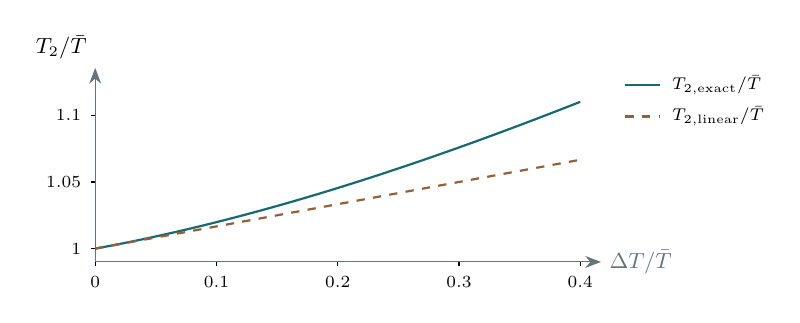
\begin{tikzpicture}[scale=.88,transform shape]
\draw[axis] (0,0)--(7.3,0) node[right] {$\Delta T/\bar T$};
\draw[axis] (0,0)--(0,2.8);
\node[above left] at (0,2.8) {$T_2/\bar T$};
\draw[thin] (0.000000,0)--(0.000000,-0.06);\node[below,font=\scriptsize] at (0.000000,-0.08) {$ 0 $};
\draw[thin] (1.750000,0)--(1.750000,-0.06);\node[below,font=\scriptsize] at (1.750000,-0.08) {$ 0.1 $};
\draw[thin] (3.500000,0)--(3.500000,-0.06);\node[below,font=\scriptsize] at (3.500000,-0.08) {$ 0.2 $};
\draw[thin] (5.250000,0)--(5.250000,-0.06);\node[below,font=\scriptsize] at (5.250000,-0.08) {$ 0.3 $};
\draw[thin] (7.000000,0)--(7.000000,-0.06);\node[below,font=\scriptsize] at (7.000000,-0.08) {$ 0.4 $};
\draw[thin] (0,0.192308)--(-.06,0.192308);\node[left,font=\scriptsize] at (-.08,0.192308) {$ 1 $};
\draw[thin] (0,1.153846)--(-.06,1.153846);\node[left,font=\scriptsize] at (-.08,1.153846) {$ 1.05 $};
\draw[thin] (0,2.115385)--(-.06,2.115385);\node[left,font=\scriptsize] at (-.08,2.115385) {$ 1.1 $};
\draw[thick,color=accent] plot coordinates {(0.0000000,0.1923077) (0.0291667,0.1976674) (0.0583333,0.2030626) (0.0875000,0.2084933) (0.1166667,0.2139594) (0.1458333,0.2194608) (0.1750000,0.2249975) (0.2041667,0.2305694) (0.2333333,0.2361764) (0.2625000,0.2418184) (0.2916667,0.2474954) (0.3208333,0.2532073) (0.3500000,0.2589541) (0.3791667,0.2647356) (0.4083333,0.2705517) (0.4375000,0.2764025) (0.4666667,0.2822878) (0.4958333,0.2882076) (0.5250000,0.2941617) (0.5541667,0.3001502) (0.5833333,0.3061729) (0.6125000,0.3122297) (0.6416667,0.3183206) (0.6708333,0.3244455) (0.7000000,0.3306043) (0.7291667,0.3367970) (0.7583333,0.3430234) (0.7875000,0.3492836) (0.8166667,0.3555773) (0.8458333,0.3619046) (0.8750000,0.3682653) (0.9041667,0.3746593) (0.9333333,0.3810867) (0.9625000,0.3875473) (0.9916667,0.3940410) (1.0208333,0.4005678) (1.0500000,0.4071275) (1.0791667,0.4137201) (1.1083333,0.4203456) (1.1375000,0.4270037) (1.1666667,0.4336945) (1.1958333,0.4404179) (1.2250000,0.4471737) (1.2541667,0.4539620) (1.2833333,0.4607825) (1.3125000,0.4676353) (1.3416667,0.4745202) (1.3708333,0.4814372) (1.4000000,0.4883862) (1.4291667,0.4953671) (1.4583333,0.5023798) (1.4875000,0.5094242) (1.5166667,0.5165003) (1.5458333,0.5236079) (1.5750000,0.5307470) (1.6041667,0.5379175) (1.6333333,0.5451193) (1.6625000,0.5523524) (1.6916667,0.5596165) (1.7208333,0.5669117) (1.7500000,0.5742379) (1.7791667,0.5815950) (1.8083333,0.5889828) (1.8375000,0.5964014) (1.8666667,0.6038505) (1.8958333,0.6113302) (1.9250000,0.6188404) (1.9541667,0.6263809) (1.9833333,0.6339516) (2.0125000,0.6415526) (2.0416667,0.6491837) (2.0708333,0.6568447) (2.1000000,0.6645357) (2.1291667,0.6722565) (2.1583333,0.6800071) (2.1875000,0.6877873) (2.2166667,0.6955971) (2.2458333,0.7034364) (2.2750000,0.7113051) (2.3041667,0.7192031) (2.3333333,0.7271303) (2.3625000,0.7350866) (2.3916667,0.7430720) (2.4208333,0.7510863) (2.4500000,0.7591295) (2.4791667,0.7672015) (2.5083333,0.7753021) (2.5375000,0.7834314) (2.5666667,0.7915891) (2.5958333,0.7997753) (2.6250000,0.8079898) (2.6541667,0.8162326) (2.6833333,0.8245035) (2.7125000,0.8328025) (2.7416667,0.8411294) (2.7708333,0.8494843) (2.8000000,0.8578669) (2.8291667,0.8662772) (2.8583333,0.8747152) (2.8875000,0.8831807) (2.9166667,0.8916736) (2.9458333,0.9001939) (2.9750000,0.9087414) (3.0041667,0.9173161) (3.0333333,0.9259179) (3.0625000,0.9345467) (3.0916667,0.9432023) (3.1208333,0.9518848) (3.1500000,0.9605940) (3.1791667,0.9693299) (3.2083333,0.9780923) (3.2375000,0.9868812) (3.2666667,0.9956964) (3.2958333,1.0045379) (3.3250000,1.0134056) (3.3541667,1.0222994) (3.3833333,1.0312191) (3.4125000,1.0401649) (3.4416667,1.0491364) (3.4708333,1.0581337) (3.5000000,1.0671566) (3.5291667,1.0762051) (3.5583333,1.0852791) (3.5875000,1.0943785) (3.6166667,1.1035032) (3.6458333,1.1126530) (3.6750000,1.1218280) (3.7041667,1.1310280) (3.7333333,1.1402530) (3.7625000,1.1495028) (3.7916667,1.1587774) (3.8208333,1.1680767) (3.8500000,1.1774005) (3.8791667,1.1867489) (3.9083333,1.1961216) (3.9375000,1.2055187) (3.9666667,1.2149400) (3.9958333,1.2243855) (4.0250000,1.2338550) (4.0541667,1.2433485) (4.0833333,1.2528659) (4.1125000,1.2624071) (4.1416667,1.2719719) (4.1708333,1.2815604) (4.2000000,1.2911725) (4.2291667,1.3008080) (4.2583333,1.3104668) (4.2875000,1.3201489) (4.3166667,1.3298542) (4.3458333,1.3395826) (4.3750000,1.3493340) (4.4041667,1.3591084) (4.4333333,1.3689055) (4.4625000,1.3787255) (4.4916667,1.3885680) (4.5208333,1.3984332) (4.5500000,1.4083209) (4.5791667,1.4182310) (4.6083333,1.4281633) (4.6375000,1.4381180) (4.6666667,1.4480948) (4.6958333,1.4580936) (4.7250000,1.4681144) (4.7541667,1.4781572) (4.7833333,1.4882217) (4.8125000,1.4983079) (4.8416667,1.5084158) (4.8708333,1.5185453) (4.9000000,1.5286962) (4.9291667,1.5388685) (4.9583333,1.5490622) (4.9875000,1.5592770) (5.0166667,1.5695130) (5.0458333,1.5797700) (5.0750000,1.5900480) (5.1041667,1.6003469) (5.1333333,1.6106666) (5.1625000,1.6210070) (5.1916667,1.6313680) (5.2208333,1.6417496) (5.2500000,1.6521517) (5.2791667,1.6625741) (5.3083333,1.6730169) (5.3375000,1.6834799) (5.3666667,1.6939630) (5.3958333,1.7044662) (5.4250000,1.7149894) (5.4541667,1.7255325) (5.4833333,1.7360953) (5.5125000,1.7466780) (5.5416667,1.7572803) (5.5708333,1.7679021) (5.6000000,1.7785435) (5.6291667,1.7892042) (5.6583333,1.7998843) (5.6875000,1.8105837) (5.7166667,1.8213022) (5.7458333,1.8320398) (5.7750000,1.8427965) (5.8041667,1.8535721) (5.8333333,1.8643665) (5.8625000,1.8751797) (5.8916667,1.8860116) (5.9208333,1.8968622) (5.9500000,1.9077312) (5.9791667,1.9186188) (6.0083333,1.9295247) (6.0375000,1.9404490) (6.0666667,1.9513915) (6.0958333,1.9623521) (6.1250000,1.9733308) (6.1541667,1.9843275) (6.1833333,1.9953422) (6.2125000,2.0063747) (6.2416667,2.0174249) (6.2708333,2.0284929) (6.3000000,2.0395785) (6.3291667,2.0506816) (6.3583333,2.0618022) (6.3875000,2.0729402) (6.4166667,2.0840955) (6.4458333,2.0952680) (6.4750000,2.1064578) (6.5041667,2.1176646) (6.5333333,2.1288884) (6.5625000,2.1401292) (6.5916667,2.1513869) (6.6208333,2.1626614) (6.6500000,2.1739525) (6.6791667,2.1852604) (6.7083333,2.1965848) (6.7375000,2.2079258) (6.7666667,2.2192831) (6.7958333,2.2306569) (6.8250000,2.2420469) (6.8541667,2.2534531) (6.8833333,2.2648755) (6.9125000,2.2763140) (6.9416667,2.2877685) (6.9708333,2.2992389) (7.0000000,2.3107251)};
\draw[thick,color=accent] (7.65,2.55)--(8.15,2.55);\node[right,font=\scriptsize] at (8.2,2.55) {$T_{2,\rm exact}/\bar T$};
\draw[thick,dashed,color=warm] plot coordinates {(0.0000000,0.1923077) (0.0291667,0.1976496) (0.0583333,0.2029915) (0.0875000,0.2083333) (0.1166667,0.2136752) (0.1458333,0.2190171) (0.1750000,0.2243590) (0.2041667,0.2297009) (0.2333333,0.2350427) (0.2625000,0.2403846) (0.2916667,0.2457265) (0.3208333,0.2510684) (0.3500000,0.2564103) (0.3791667,0.2617521) (0.4083333,0.2670940) (0.4375000,0.2724359) (0.4666667,0.2777778) (0.4958333,0.2831197) (0.5250000,0.2884615) (0.5541667,0.2938034) (0.5833333,0.2991453) (0.6125000,0.3044872) (0.6416667,0.3098291) (0.6708333,0.3151709) (0.7000000,0.3205128) (0.7291667,0.3258547) (0.7583333,0.3311966) (0.7875000,0.3365385) (0.8166667,0.3418803) (0.8458333,0.3472222) (0.8750000,0.3525641) (0.9041667,0.3579060) (0.9333333,0.3632479) (0.9625000,0.3685897) (0.9916667,0.3739316) (1.0208333,0.3792735) (1.0500000,0.3846154) (1.0791667,0.3899573) (1.1083333,0.3952991) (1.1375000,0.4006410) (1.1666667,0.4059829) (1.1958333,0.4113248) (1.2250000,0.4166667) (1.2541667,0.4220085) (1.2833333,0.4273504) (1.3125000,0.4326923) (1.3416667,0.4380342) (1.3708333,0.4433761) (1.4000000,0.4487179) (1.4291667,0.4540598) (1.4583333,0.4594017) (1.4875000,0.4647436) (1.5166667,0.4700855) (1.5458333,0.4754274) (1.5750000,0.4807692) (1.6041667,0.4861111) (1.6333333,0.4914530) (1.6625000,0.4967949) (1.6916667,0.5021368) (1.7208333,0.5074786) (1.7500000,0.5128205) (1.7791667,0.5181624) (1.8083333,0.5235043) (1.8375000,0.5288462) (1.8666667,0.5341880) (1.8958333,0.5395299) (1.9250000,0.5448718) (1.9541667,0.5502137) (1.9833333,0.5555556) (2.0125000,0.5608974) (2.0416667,0.5662393) (2.0708333,0.5715812) (2.1000000,0.5769231) (2.1291667,0.5822650) (2.1583333,0.5876068) (2.1875000,0.5929487) (2.2166667,0.5982906) (2.2458333,0.6036325) (2.2750000,0.6089744) (2.3041667,0.6143162) (2.3333333,0.6196581) (2.3625000,0.6250000) (2.3916667,0.6303419) (2.4208333,0.6356838) (2.4500000,0.6410256) (2.4791667,0.6463675) (2.5083333,0.6517094) (2.5375000,0.6570513) (2.5666667,0.6623932) (2.5958333,0.6677350) (2.6250000,0.6730769) (2.6541667,0.6784188) (2.6833333,0.6837607) (2.7125000,0.6891026) (2.7416667,0.6944444) (2.7708333,0.6997863) (2.8000000,0.7051282) (2.8291667,0.7104701) (2.8583333,0.7158120) (2.8875000,0.7211538) (2.9166667,0.7264957) (2.9458333,0.7318376) (2.9750000,0.7371795) (3.0041667,0.7425214) (3.0333333,0.7478632) (3.0625000,0.7532051) (3.0916667,0.7585470) (3.1208333,0.7638889) (3.1500000,0.7692308) (3.1791667,0.7745726) (3.2083333,0.7799145) (3.2375000,0.7852564) (3.2666667,0.7905983) (3.2958333,0.7959402) (3.3250000,0.8012821) (3.3541667,0.8066239) (3.3833333,0.8119658) (3.4125000,0.8173077) (3.4416667,0.8226496) (3.4708333,0.8279915) (3.5000000,0.8333333) (3.5291667,0.8386752) (3.5583333,0.8440171) (3.5875000,0.8493590) (3.6166667,0.8547009) (3.6458333,0.8600427) (3.6750000,0.8653846) (3.7041667,0.8707265) (3.7333333,0.8760684) (3.7625000,0.8814103) (3.7916667,0.8867521) (3.8208333,0.8920940) (3.8500000,0.8974359) (3.8791667,0.9027778) (3.9083333,0.9081197) (3.9375000,0.9134615) (3.9666667,0.9188034) (3.9958333,0.9241453) (4.0250000,0.9294872) (4.0541667,0.9348291) (4.0833333,0.9401709) (4.1125000,0.9455128) (4.1416667,0.9508547) (4.1708333,0.9561966) (4.2000000,0.9615385) (4.2291667,0.9668803) (4.2583333,0.9722222) (4.2875000,0.9775641) (4.3166667,0.9829060) (4.3458333,0.9882479) (4.3750000,0.9935897) (4.4041667,0.9989316) (4.4333333,1.0042735) (4.4625000,1.0096154) (4.4916667,1.0149573) (4.5208333,1.0202991) (4.5500000,1.0256410) (4.5791667,1.0309829) (4.6083333,1.0363248) (4.6375000,1.0416667) (4.6666667,1.0470085) (4.6958333,1.0523504) (4.7250000,1.0576923) (4.7541667,1.0630342) (4.7833333,1.0683761) (4.8125000,1.0737179) (4.8416667,1.0790598) (4.8708333,1.0844017) (4.9000000,1.0897436) (4.9291667,1.0950855) (4.9583333,1.1004274) (4.9875000,1.1057692) (5.0166667,1.1111111) (5.0458333,1.1164530) (5.0750000,1.1217949) (5.1041667,1.1271368) (5.1333333,1.1324786) (5.1625000,1.1378205) (5.1916667,1.1431624) (5.2208333,1.1485043) (5.2500000,1.1538462) (5.2791667,1.1591880) (5.3083333,1.1645299) (5.3375000,1.1698718) (5.3666667,1.1752137) (5.3958333,1.1805556) (5.4250000,1.1858974) (5.4541667,1.1912393) (5.4833333,1.1965812) (5.5125000,1.2019231) (5.5416667,1.2072650) (5.5708333,1.2126068) (5.6000000,1.2179487) (5.6291667,1.2232906) (5.6583333,1.2286325) (5.6875000,1.2339744) (5.7166667,1.2393162) (5.7458333,1.2446581) (5.7750000,1.2500000) (5.8041667,1.2553419) (5.8333333,1.2606838) (5.8625000,1.2660256) (5.8916667,1.2713675) (5.9208333,1.2767094) (5.9500000,1.2820513) (5.9791667,1.2873932) (6.0083333,1.2927350) (6.0375000,1.2980769) (6.0666667,1.3034188) (6.0958333,1.3087607) (6.1250000,1.3141026) (6.1541667,1.3194444) (6.1833333,1.3247863) (6.2125000,1.3301282) (6.2416667,1.3354701) (6.2708333,1.3408120) (6.3000000,1.3461538) (6.3291667,1.3514957) (6.3583333,1.3568376) (6.3875000,1.3621795) (6.4166667,1.3675214) (6.4458333,1.3728632) (6.4750000,1.3782051) (6.5041667,1.3835470) (6.5333333,1.3888889) (6.5625000,1.3942308) (6.5916667,1.3995726) (6.6208333,1.4049145) (6.6500000,1.4102564) (6.6791667,1.4155983) (6.7083333,1.4209402) (6.7375000,1.4262821) (6.7666667,1.4316239) (6.7958333,1.4369658) (6.8250000,1.4423077) (6.8541667,1.4476496) (6.8833333,1.4529915) (6.9125000,1.4583333) (6.9416667,1.4636752) (6.9708333,1.4690171) (7.0000000,1.4743590)};
\draw[thick,dashed,color=warm] (7.65,2.0999999999999996)--(8.15,2.0999999999999996);\node[right,font=\scriptsize] at (8.2,2.0999999999999996) {$T_{2,\rm linear}/\bar T$};
\end{tikzpicture}
\figcaption{变图近1.4V3\quad 两内板情形中靠热端内板的准确温度与小温差近似}
\end{minipage}\end{center}
\item \textbf{所有表面为同一漫灰体。}各面发射率为$\varepsilon$，无限平行、各板两面等温，求插$n$板的净流。

两相对面的出射度满足$J_a=\varepsilon\sigma T_a^4+(1-\varepsilon)J_b$、$J_b=\varepsilon\sigma T_b^4+(1-\varepsilon)J_a$。相减得$(2-\varepsilon)(J_a-J_b)=\varepsilon\sigma(T_a^4-T_b^4)$，所以单隙$q=\sigma(T_a^4-T_b^4)/(2/\varepsilon-1)$。相同的$n+1$个间隙串联，
\[
 q=\frac{\sigma(T_h^4-T_c^4)}
 {(n+1)(2/\varepsilon-1)}.
\]
变图近1.4V4取$n=2$，仍以两黑端面直接交换的$q_0=\sigma(T_h^4-T_c^4)$为比较标尺，画$q/q_0$随$\varepsilon$的变化。若将相同灰端面不插屏的净流记为$q_{0,\mathrm{gray}}=q_0/(2/\varepsilon-1)$，则$q/q_{0,\mathrm{gray}}=1/(n+1)$。前一个比值同时显示表面发射率与屏数的作用，后一个比值显示同种灰端面之间增加屏数的作用。
\begin{center}\begin{minipage}{.98\linewidth}\centering
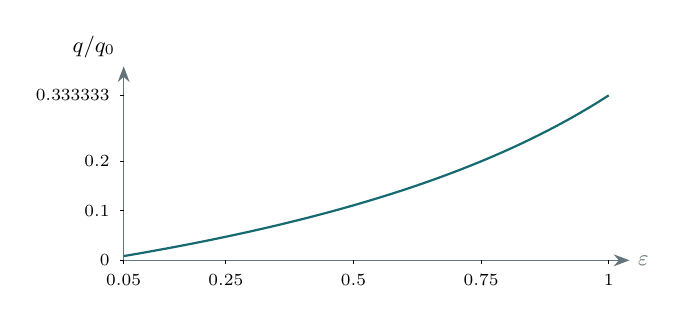
\begin{tikzpicture}[scale=.88,transform shape]
\draw[axis] (0,0.0)--(7.3,0.0) node[right] {$\varepsilon$};
\draw[axis] (0,0)--(0,2.8);
\node[above left] at (0,2.8) {$q/q_0$};
\draw[thin] (0.000000,0.0)--(0.000000,-0.06);\node[below,font=\scriptsize] at (0.000000,-0.08) {$ 0.05 $};
\draw[thin] (1.473684,0.0)--(1.473684,-0.06);\node[below,font=\scriptsize] at (1.473684,-0.08) {$ 0.25 $};
\draw[thin] (3.315789,0.0)--(3.315789,-0.06);\node[below,font=\scriptsize] at (3.315789,-0.08) {$ 0.5 $};
\draw[thin] (5.157895,0.0)--(5.157895,-0.06);\node[below,font=\scriptsize] at (5.157895,-0.08) {$ 0.75 $};
\draw[thin] (7.000000,0.0)--(7.000000,-0.06);\node[below,font=\scriptsize] at (7.000000,-0.08) {$ 1 $};
\draw[thin] (0,0.000000)--(-.06,0.000000);\node[left,font=\scriptsize] at (-.08,0.000000) {$ 0 $};
\draw[thin] (0,0.714286)--(-.06,0.714286);\node[left,font=\scriptsize] at (-.08,0.714286) {$ 0.1 $};
\draw[thin] (0,1.428571)--(-.06,1.428571);\node[left,font=\scriptsize] at (-.08,1.428571) {$ 0.2 $};
\draw[thin] (0,2.380952)--(-.06,2.380952);\node[left,font=\scriptsize] at (-.08,2.380952) {$ 0.333333 $};
\draw[thick,color=accent] plot coordinates {(0.0000000,0.0610501) (0.0291667,0.0660172) (0.0583333,0.0710046) (0.0875000,0.0760123) (0.1166667,0.0810406) (0.1458333,0.0860895) (0.1750000,0.0911591) (0.2041667,0.0962496) (0.2333333,0.1013611) (0.2625000,0.1064938) (0.2916667,0.1116477) (0.3208333,0.1168230) (0.3500000,0.1220199) (0.3791667,0.1272384) (0.4083333,0.1324788) (0.4375000,0.1377410) (0.4666667,0.1430254) (0.4958333,0.1483320) (0.5250000,0.1536609) (0.5541667,0.1590124) (0.5833333,0.1643865) (0.6125000,0.1697833) (0.6416667,0.1752032) (0.6708333,0.1806461) (0.7000000,0.1861122) (0.7291667,0.1916017) (0.7583333,0.1971147) (0.7875000,0.2026514) (0.8166667,0.2082120) (0.8458333,0.2137965) (0.8750000,0.2194052) (0.9041667,0.2250381) (0.9333333,0.2306956) (0.9625000,0.2363776) (0.9916667,0.2420844) (1.0208333,0.2478162) (1.0500000,0.2535731) (1.0791667,0.2593552) (1.1083333,0.2651628) (1.1375000,0.2709960) (1.1666667,0.2768549) (1.1958333,0.2827398) (1.2250000,0.2886508) (1.2541667,0.2945882) (1.2833333,0.3005519) (1.3125000,0.3065424) (1.3416667,0.3125596) (1.3708333,0.3186039) (1.4000000,0.3246753) (1.4291667,0.3307741) (1.4583333,0.3369005) (1.4875000,0.3430546) (1.5166667,0.3492367) (1.5458333,0.3554469) (1.5750000,0.3616854) (1.6041667,0.3679524) (1.6333333,0.3742481) (1.6625000,0.3805727) (1.6916667,0.3869264) (1.7208333,0.3933094) (1.7500000,0.3997219) (1.7791667,0.4061642) (1.8083333,0.4126363) (1.8375000,0.4191386) (1.8666667,0.4256713) (1.8958333,0.4322344) (1.9250000,0.4388284) (1.9541667,0.4454533) (1.9833333,0.4521095) (2.0125000,0.4587970) (2.0416667,0.4655162) (2.0708333,0.4722673) (2.1000000,0.4790505) (2.1291667,0.4858660) (2.1583333,0.4927141) (2.1875000,0.4995949) (2.2166667,0.5065088) (2.2458333,0.5134560) (2.2750000,0.5204367) (2.3041667,0.5274511) (2.3333333,0.5344995) (2.3625000,0.5415822) (2.3916667,0.5486994) (2.4208333,0.5558513) (2.4500000,0.5630382) (2.4791667,0.5702604) (2.5083333,0.5775181) (2.5375000,0.5848116) (2.5666667,0.5921411) (2.5958333,0.5995070) (2.6250000,0.6069094) (2.6541667,0.6143487) (2.6833333,0.6218252) (2.7125000,0.6293391) (2.7416667,0.6368906) (2.7708333,0.6444802) (2.8000000,0.6521080) (2.8291667,0.6597744) (2.8583333,0.6674796) (2.8875000,0.6752240) (2.9166667,0.6830078) (2.9458333,0.6908314) (2.9750000,0.6986950) (3.0041667,0.7065990) (3.0333333,0.7145437) (3.0625000,0.7225293) (3.0916667,0.7305563) (3.1208333,0.7386249) (3.1500000,0.7467355) (3.1791667,0.7548883) (3.2083333,0.7630838) (3.2375000,0.7713222) (3.2666667,0.7796039) (3.2958333,0.7879292) (3.3250000,0.7962985) (3.3541667,0.8047121) (3.3833333,0.8131704) (3.4125000,0.8216738) (3.4416667,0.8302225) (3.4708333,0.8388170) (3.5000000,0.8474576) (3.5291667,0.8561448) (3.5583333,0.8648788) (3.5875000,0.8736600) (3.6166667,0.8824889) (3.6458333,0.8913659) (3.6750000,0.9002912) (3.7041667,0.9092654) (3.7333333,0.9182888) (3.7625000,0.9273618) (3.7916667,0.9364849) (3.8208333,0.9456584) (3.8500000,0.9548828) (3.8791667,0.9641585) (3.9083333,0.9734860) (3.9375000,0.9828656) (3.9666667,0.9922977) (3.9958333,1.0017830) (4.0250000,1.0113217) (4.0541667,1.0209144) (4.0833333,1.0305615) (4.1125000,1.0402634) (4.1416667,1.0500207) (4.1708333,1.0598338) (4.2000000,1.0697032) (4.2291667,1.0796294) (4.2583333,1.0896129) (4.2875000,1.0996541) (4.3166667,1.1097536) (4.3458333,1.1199119) (4.3750000,1.1301295) (4.4041667,1.1404069) (4.4333333,1.1507446) (4.4625000,1.1611432) (4.4916667,1.1716032) (4.5208333,1.1821252) (4.5500000,1.1927097) (4.5791667,1.2033573) (4.6083333,1.2140685) (4.6375000,1.2248439) (4.6666667,1.2356841) (4.6958333,1.2465897) (4.7250000,1.2575613) (4.7541667,1.2685994) (4.7833333,1.2797047) (4.8125000,1.2908778) (4.8416667,1.3021193) (4.8708333,1.3134298) (4.9000000,1.3248101) (4.9291667,1.3362606) (4.9583333,1.3477822) (4.9875000,1.3593754) (5.0166667,1.3710409) (5.0458333,1.3827794) (5.0750000,1.3945915) (5.1041667,1.4064781) (5.1333333,1.4184397) (5.1625000,1.4304771) (5.1916667,1.4425911) (5.2208333,1.4547823) (5.2500000,1.4670515) (5.2791667,1.4793994) (5.3083333,1.4918268) (5.3375000,1.5043345) (5.3666667,1.5169233) (5.3958333,1.5295939) (5.4250000,1.5423471) (5.4541667,1.5551838) (5.4833333,1.5681048) (5.5125000,1.5811109) (5.5416667,1.5942029) (5.5708333,1.6073817) (5.6000000,1.6206483) (5.6291667,1.6340033) (5.6583333,1.6474478) (5.6875000,1.6609827) (5.7166667,1.6746088) (5.7458333,1.6883271) (5.7750000,1.7021385) (5.8041667,1.7160440) (5.8333333,1.7300445) (5.8625000,1.7441411) (5.8916667,1.7583346) (5.9208333,1.7726262) (5.9500000,1.7870168) (5.9791667,1.8015074) (6.0083333,1.8160992) (6.0375000,1.8307931) (6.0666667,1.8455903) (6.0958333,1.8604918) (6.1250000,1.8754988) (6.1541667,1.8906123) (6.1833333,1.9058336) (6.2125000,1.9211637) (6.2416667,1.9366039) (6.2708333,1.9521553) (6.3000000,1.9678191) (6.3291667,1.9835966) (6.3583333,1.9994889) (6.3875000,2.0154975) (6.4166667,2.0316235) (6.4458333,2.0478682) (6.4750000,2.0642329) (6.5041667,2.0807191) (6.5333333,2.0973280) (6.5625000,2.1140610) (6.5916667,2.1309195) (6.6208333,2.1479049) (6.6500000,2.1650188) (6.6791667,2.1822624) (6.7083333,2.1996374) (6.7375000,2.2171452) (6.7666667,2.2347873) (6.7958333,2.2525653) (6.8250000,2.2704808) (6.8541667,2.2885354) (6.8833333,2.3067307) (6.9125000,2.3250684) (6.9416667,2.3435501) (6.9708333,2.3621775) (7.0000000,2.3809524)};
\end{tikzpicture}
\figcaption{变图近1.4V4\quad 所有表面为同一灰体且插两屏时的净传热}
\end{minipage}\end{center}
\item \textbf{黑端面之间插低发射率薄屏。}两端为黑面，只插一块两面发射率均为$\varepsilon$的等温灰屏，求屏温和传热。

黑面到灰屏的单隙净流为$\varepsilon\sigma(T_h^4-T_m^4)$，灰屏到黑冷端为$\varepsilon\sigma(T_m^4-T_c^4)$。稳态两者相等，给$T_m^4=(T_h^4+T_c^4)/2$，所以$q/q_0=\varepsilon/2$。变图近1.4V5画这一比例；$\varepsilon=0.1$给$1/20$，同样一块黑屏则为$1/2$。中间温度相同，而辐射交换系数不同。
\begin{center}\begin{minipage}{.98\linewidth}\centering
\begin{tikzpicture}[scale=.88,transform shape]
\draw[axis] (0,0.0)--(7.3,0.0) node[right] {$\varepsilon$};
\draw[axis] (0,0)--(0,2.8);
\node[above left] at (0,2.8) {$q/q_0$};
\draw[thin] (0.000000,0.0)--(0.000000,-0.06);\node[below,font=\scriptsize] at (0.000000,-0.08) {$ 0 $};
\draw[thin] (0.700000,0.0)--(0.700000,-0.06);\node[below,font=\scriptsize] at (0.700000,-0.08) {$ 0.1 $};
\draw[thin] (3.500000,0.0)--(3.500000,-0.06);\node[below,font=\scriptsize] at (3.500000,-0.08) {$ 0.5 $};
\draw[thin] (7.000000,0.0)--(7.000000,-0.06);\node[below,font=\scriptsize] at (7.000000,-0.08) {$ 1 $};
\draw[thin] (0,0.000000)--(-.06,0.000000);\node[left,font=\scriptsize] at (-.08,0.000000) {$ 0 $};
\draw[thin] (0,0.227273)--(-.06,0.227273);\node[left,font=\scriptsize] at (-.08,0.227273) {$ 0.05 $};
\draw[thin] (0,1.136364)--(-.06,1.136364);\node[left,font=\scriptsize] at (-.08,1.136364) {$ 0.25 $};
\draw[thin] (0,2.272727)--(-.06,2.272727);\node[left,font=\scriptsize] at (-.08,2.272727) {$ 0.5 $};
\draw[thick,color=accent] plot coordinates {(0.0000000,0.0000000) (0.0291667,0.0094697) (0.0583333,0.0189394) (0.0875000,0.0284091) (0.1166667,0.0378788) (0.1458333,0.0473485) (0.1750000,0.0568182) (0.2041667,0.0662879) (0.2333333,0.0757576) (0.2625000,0.0852273) (0.2916667,0.0946970) (0.3208333,0.1041667) (0.3500000,0.1136364) (0.3791667,0.1231061) (0.4083333,0.1325758) (0.4375000,0.1420455) (0.4666667,0.1515152) (0.4958333,0.1609848) (0.5250000,0.1704545) (0.5541667,0.1799242) (0.5833333,0.1893939) (0.6125000,0.1988636) (0.6416667,0.2083333) (0.6708333,0.2178030) (0.7000000,0.2272727) (0.7291667,0.2367424) (0.7583333,0.2462121) (0.7875000,0.2556818) (0.8166667,0.2651515) (0.8458333,0.2746212) (0.8750000,0.2840909) (0.9041667,0.2935606) (0.9333333,0.3030303) (0.9625000,0.3125000) (0.9916667,0.3219697) (1.0208333,0.3314394) (1.0500000,0.3409091) (1.0791667,0.3503788) (1.1083333,0.3598485) (1.1375000,0.3693182) (1.1666667,0.3787879) (1.1958333,0.3882576) (1.2250000,0.3977273) (1.2541667,0.4071970) (1.2833333,0.4166667) (1.3125000,0.4261364) (1.3416667,0.4356061) (1.3708333,0.4450758) (1.4000000,0.4545455) (1.4291667,0.4640152) (1.4583333,0.4734848) (1.4875000,0.4829545) (1.5166667,0.4924242) (1.5458333,0.5018939) (1.5750000,0.5113636) (1.6041667,0.5208333) (1.6333333,0.5303030) (1.6625000,0.5397727) (1.6916667,0.5492424) (1.7208333,0.5587121) (1.7500000,0.5681818) (1.7791667,0.5776515) (1.8083333,0.5871212) (1.8375000,0.5965909) (1.8666667,0.6060606) (1.8958333,0.6155303) (1.9250000,0.6250000) (1.9541667,0.6344697) (1.9833333,0.6439394) (2.0125000,0.6534091) (2.0416667,0.6628788) (2.0708333,0.6723485) (2.1000000,0.6818182) (2.1291667,0.6912879) (2.1583333,0.7007576) (2.1875000,0.7102273) (2.2166667,0.7196970) (2.2458333,0.7291667) (2.2750000,0.7386364) (2.3041667,0.7481061) (2.3333333,0.7575758) (2.3625000,0.7670455) (2.3916667,0.7765152) (2.4208333,0.7859848) (2.4500000,0.7954545) (2.4791667,0.8049242) (2.5083333,0.8143939) (2.5375000,0.8238636) (2.5666667,0.8333333) (2.5958333,0.8428030) (2.6250000,0.8522727) (2.6541667,0.8617424) (2.6833333,0.8712121) (2.7125000,0.8806818) (2.7416667,0.8901515) (2.7708333,0.8996212) (2.8000000,0.9090909) (2.8291667,0.9185606) (2.8583333,0.9280303) (2.8875000,0.9375000) (2.9166667,0.9469697) (2.9458333,0.9564394) (2.9750000,0.9659091) (3.0041667,0.9753788) (3.0333333,0.9848485) (3.0625000,0.9943182) (3.0916667,1.0037879) (3.1208333,1.0132576) (3.1500000,1.0227273) (3.1791667,1.0321970) (3.2083333,1.0416667) (3.2375000,1.0511364) (3.2666667,1.0606061) (3.2958333,1.0700758) (3.3250000,1.0795455) (3.3541667,1.0890152) (3.3833333,1.0984848) (3.4125000,1.1079545) (3.4416667,1.1174242) (3.4708333,1.1268939) (3.5000000,1.1363636) (3.5291667,1.1458333) (3.5583333,1.1553030) (3.5875000,1.1647727) (3.6166667,1.1742424) (3.6458333,1.1837121) (3.6750000,1.1931818) (3.7041667,1.2026515) (3.7333333,1.2121212) (3.7625000,1.2215909) (3.7916667,1.2310606) (3.8208333,1.2405303) (3.8500000,1.2500000) (3.8791667,1.2594697) (3.9083333,1.2689394) (3.9375000,1.2784091) (3.9666667,1.2878788) (3.9958333,1.2973485) (4.0250000,1.3068182) (4.0541667,1.3162879) (4.0833333,1.3257576) (4.1125000,1.3352273) (4.1416667,1.3446970) (4.1708333,1.3541667) (4.2000000,1.3636364) (4.2291667,1.3731061) (4.2583333,1.3825758) (4.2875000,1.3920455) (4.3166667,1.4015152) (4.3458333,1.4109848) (4.3750000,1.4204545) (4.4041667,1.4299242) (4.4333333,1.4393939) (4.4625000,1.4488636) (4.4916667,1.4583333) (4.5208333,1.4678030) (4.5500000,1.4772727) (4.5791667,1.4867424) (4.6083333,1.4962121) (4.6375000,1.5056818) (4.6666667,1.5151515) (4.6958333,1.5246212) (4.7250000,1.5340909) (4.7541667,1.5435606) (4.7833333,1.5530303) (4.8125000,1.5625000) (4.8416667,1.5719697) (4.8708333,1.5814394) (4.9000000,1.5909091) (4.9291667,1.6003788) (4.9583333,1.6098485) (4.9875000,1.6193182) (5.0166667,1.6287879) (5.0458333,1.6382576) (5.0750000,1.6477273) (5.1041667,1.6571970) (5.1333333,1.6666667) (5.1625000,1.6761364) (5.1916667,1.6856061) (5.2208333,1.6950758) (5.2500000,1.7045455) (5.2791667,1.7140152) (5.3083333,1.7234848) (5.3375000,1.7329545) (5.3666667,1.7424242) (5.3958333,1.7518939) (5.4250000,1.7613636) (5.4541667,1.7708333) (5.4833333,1.7803030) (5.5125000,1.7897727) (5.5416667,1.7992424) (5.5708333,1.8087121) (5.6000000,1.8181818) (5.6291667,1.8276515) (5.6583333,1.8371212) (5.6875000,1.8465909) (5.7166667,1.8560606) (5.7458333,1.8655303) (5.7750000,1.8750000) (5.8041667,1.8844697) (5.8333333,1.8939394) (5.8625000,1.9034091) (5.8916667,1.9128788) (5.9208333,1.9223485) (5.9500000,1.9318182) (5.9791667,1.9412879) (6.0083333,1.9507576) (6.0375000,1.9602273) (6.0666667,1.9696970) (6.0958333,1.9791667) (6.1250000,1.9886364) (6.1541667,1.9981061) (6.1833333,2.0075758) (6.2125000,2.0170455) (6.2416667,2.0265152) (6.2708333,2.0359848) (6.3000000,2.0454545) (6.3291667,2.0549242) (6.3583333,2.0643939) (6.3875000,2.0738636) (6.4166667,2.0833333) (6.4458333,2.0928030) (6.4750000,2.1022727) (6.5041667,2.1117424) (6.5333333,2.1212121) (6.5625000,2.1306818) (6.5916667,2.1401515) (6.6208333,2.1496212) (6.6500000,2.1590909) (6.6791667,2.1685606) (6.7083333,2.1780303) (6.7375000,2.1875000) (6.7666667,2.1969697) (6.7958333,2.2064394) (6.8250000,2.2159091) (6.8541667,2.2253788) (6.8833333,2.2348485) (6.9125000,2.2443182) (6.9416667,2.2537879) (6.9708333,2.2632576) (7.0000000,2.2727273)};
\end{tikzpicture}
\figcaption{变图近1.4V5\quad 两端黑面之间只插一块灰屏}
\end{minipage}\end{center}
\item \textbf{中间板另有外加加热。}只插一块黑板，外加单位面积功率为$q_s$，求温度以及两侧净流方向。

稳态为$\sigma(T_h^4+T_c^4-2T_m^4)+q_s=0$，所以
\[
 T_m^4=\frac{T_h^4+T_c^4+q_s/\sigma}{2},\quad
 q_L=\frac{q_0-q_s}{2},\quad q_R=\frac{q_0+q_s}{2}.
\]
正方向均取热端到冷端，$q_R-q_L=q_s$。变图近1.4V6以$s=q_s/q_0$画两流，$s>1$时$q_L<0$，内板还向热端供热；外加能量改变了内板温度与流量连续式。
\begin{center}\begin{minipage}{.98\linewidth}\centering
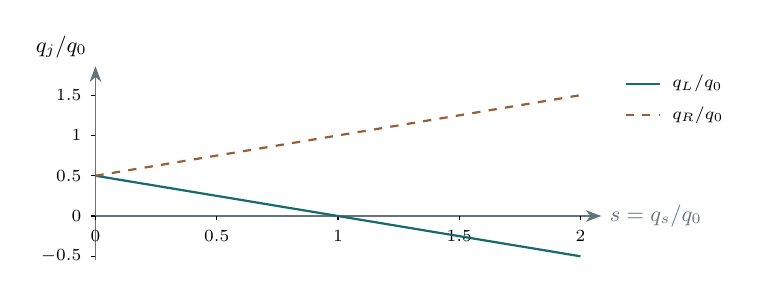
\begin{tikzpicture}[scale=.88,transform shape]
\draw[axis] (0,0.6395348837209301)--(7.3,0.6395348837209301) node[right] {$s=q_s/q_0$};
\draw[axis] (0,0)--(0,2.8);
\node[above left] at (0,2.8) {$q_j/q_0$};
\draw[thin] (0.000000,0.6395348837209301)--(0.000000,0.5795348837209302);\node[below,font=\scriptsize] at (0.000000,0.5595348837209302) {$ 0 $};
\draw[thin] (1.750000,0.6395348837209301)--(1.750000,0.5795348837209302);\node[below,font=\scriptsize] at (1.750000,0.5595348837209302) {$ 0.5 $};
\draw[thin] (3.500000,0.6395348837209301)--(3.500000,0.5795348837209302);\node[below,font=\scriptsize] at (3.500000,0.5595348837209302) {$ 1 $};
\draw[thin] (5.250000,0.6395348837209301)--(5.250000,0.5795348837209302);\node[below,font=\scriptsize] at (5.250000,0.5595348837209302) {$ 1.5 $};
\draw[thin] (7.000000,0.6395348837209301)--(7.000000,0.5795348837209302);\node[below,font=\scriptsize] at (7.000000,0.5595348837209302) {$ 2 $};
\draw[thin] (0,0.058140)--(-.06,0.058140);\node[left,font=\scriptsize] at (-.08,0.058140) {$ -0.5 $};
\draw[thin] (0,0.639535)--(-.06,0.639535);\node[left,font=\scriptsize] at (-.08,0.639535) {$ 0 $};
\draw[thin] (0,1.220930)--(-.06,1.220930);\node[left,font=\scriptsize] at (-.08,1.220930) {$ 0.5 $};
\draw[thin] (0,1.802326)--(-.06,1.802326);\node[left,font=\scriptsize] at (-.08,1.802326) {$ 1 $};
\draw[thin] (0,2.383721)--(-.06,2.383721);\node[left,font=\scriptsize] at (-.08,2.383721) {$ 1.5 $};
\draw[thick,color=accent] plot coordinates {(0.0000000,1.2209302) (0.0291667,1.2160853) (0.0583333,1.2112403) (0.0875000,1.2063953) (0.1166667,1.2015504) (0.1458333,1.1967054) (0.1750000,1.1918605) (0.2041667,1.1870155) (0.2333333,1.1821705) (0.2625000,1.1773256) (0.2916667,1.1724806) (0.3208333,1.1676357) (0.3500000,1.1627907) (0.3791667,1.1579457) (0.4083333,1.1531008) (0.4375000,1.1482558) (0.4666667,1.1434109) (0.4958333,1.1385659) (0.5250000,1.1337209) (0.5541667,1.1288760) (0.5833333,1.1240310) (0.6125000,1.1191860) (0.6416667,1.1143411) (0.6708333,1.1094961) (0.7000000,1.1046512) (0.7291667,1.0998062) (0.7583333,1.0949612) (0.7875000,1.0901163) (0.8166667,1.0852713) (0.8458333,1.0804264) (0.8750000,1.0755814) (0.9041667,1.0707364) (0.9333333,1.0658915) (0.9625000,1.0610465) (0.9916667,1.0562016) (1.0208333,1.0513566) (1.0500000,1.0465116) (1.0791667,1.0416667) (1.1083333,1.0368217) (1.1375000,1.0319767) (1.1666667,1.0271318) (1.1958333,1.0222868) (1.2250000,1.0174419) (1.2541667,1.0125969) (1.2833333,1.0077519) (1.3125000,1.0029070) (1.3416667,0.9980620) (1.3708333,0.9932171) (1.4000000,0.9883721) (1.4291667,0.9835271) (1.4583333,0.9786822) (1.4875000,0.9738372) (1.5166667,0.9689922) (1.5458333,0.9641473) (1.5750000,0.9593023) (1.6041667,0.9544574) (1.6333333,0.9496124) (1.6625000,0.9447674) (1.6916667,0.9399225) (1.7208333,0.9350775) (1.7500000,0.9302326) (1.7791667,0.9253876) (1.8083333,0.9205426) (1.8375000,0.9156977) (1.8666667,0.9108527) (1.8958333,0.9060078) (1.9250000,0.9011628) (1.9541667,0.8963178) (1.9833333,0.8914729) (2.0125000,0.8866279) (2.0416667,0.8817829) (2.0708333,0.8769380) (2.1000000,0.8720930) (2.1291667,0.8672481) (2.1583333,0.8624031) (2.1875000,0.8575581) (2.2166667,0.8527132) (2.2458333,0.8478682) (2.2750000,0.8430233) (2.3041667,0.8381783) (2.3333333,0.8333333) (2.3625000,0.8284884) (2.3916667,0.8236434) (2.4208333,0.8187984) (2.4500000,0.8139535) (2.4791667,0.8091085) (2.5083333,0.8042636) (2.5375000,0.7994186) (2.5666667,0.7945736) (2.5958333,0.7897287) (2.6250000,0.7848837) (2.6541667,0.7800388) (2.6833333,0.7751938) (2.7125000,0.7703488) (2.7416667,0.7655039) (2.7708333,0.7606589) (2.8000000,0.7558140) (2.8291667,0.7509690) (2.8583333,0.7461240) (2.8875000,0.7412791) (2.9166667,0.7364341) (2.9458333,0.7315891) (2.9750000,0.7267442) (3.0041667,0.7218992) (3.0333333,0.7170543) (3.0625000,0.7122093) (3.0916667,0.7073643) (3.1208333,0.7025194) (3.1500000,0.6976744) (3.1791667,0.6928295) (3.2083333,0.6879845) (3.2375000,0.6831395) (3.2666667,0.6782946) (3.2958333,0.6734496) (3.3250000,0.6686047) (3.3541667,0.6637597) (3.3833333,0.6589147) (3.4125000,0.6540698) (3.4416667,0.6492248) (3.4708333,0.6443798) (3.5000000,0.6395349) (3.5291667,0.6346899) (3.5583333,0.6298450) (3.5875000,0.6250000) (3.6166667,0.6201550) (3.6458333,0.6153101) (3.6750000,0.6104651) (3.7041667,0.6056202) (3.7333333,0.6007752) (3.7625000,0.5959302) (3.7916667,0.5910853) (3.8208333,0.5862403) (3.8500000,0.5813953) (3.8791667,0.5765504) (3.9083333,0.5717054) (3.9375000,0.5668605) (3.9666667,0.5620155) (3.9958333,0.5571705) (4.0250000,0.5523256) (4.0541667,0.5474806) (4.0833333,0.5426357) (4.1125000,0.5377907) (4.1416667,0.5329457) (4.1708333,0.5281008) (4.2000000,0.5232558) (4.2291667,0.5184109) (4.2583333,0.5135659) (4.2875000,0.5087209) (4.3166667,0.5038760) (4.3458333,0.4990310) (4.3750000,0.4941860) (4.4041667,0.4893411) (4.4333333,0.4844961) (4.4625000,0.4796512) (4.4916667,0.4748062) (4.5208333,0.4699612) (4.5500000,0.4651163) (4.5791667,0.4602713) (4.6083333,0.4554264) (4.6375000,0.4505814) (4.6666667,0.4457364) (4.6958333,0.4408915) (4.7250000,0.4360465) (4.7541667,0.4312016) (4.7833333,0.4263566) (4.8125000,0.4215116) (4.8416667,0.4166667) (4.8708333,0.4118217) (4.9000000,0.4069767) (4.9291667,0.4021318) (4.9583333,0.3972868) (4.9875000,0.3924419) (5.0166667,0.3875969) (5.0458333,0.3827519) (5.0750000,0.3779070) (5.1041667,0.3730620) (5.1333333,0.3682171) (5.1625000,0.3633721) (5.1916667,0.3585271) (5.2208333,0.3536822) (5.2500000,0.3488372) (5.2791667,0.3439922) (5.3083333,0.3391473) (5.3375000,0.3343023) (5.3666667,0.3294574) (5.3958333,0.3246124) (5.4250000,0.3197674) (5.4541667,0.3149225) (5.4833333,0.3100775) (5.5125000,0.3052326) (5.5416667,0.3003876) (5.5708333,0.2955426) (5.6000000,0.2906977) (5.6291667,0.2858527) (5.6583333,0.2810078) (5.6875000,0.2761628) (5.7166667,0.2713178) (5.7458333,0.2664729) (5.7750000,0.2616279) (5.8041667,0.2567829) (5.8333333,0.2519380) (5.8625000,0.2470930) (5.8916667,0.2422481) (5.9208333,0.2374031) (5.9500000,0.2325581) (5.9791667,0.2277132) (6.0083333,0.2228682) (6.0375000,0.2180233) (6.0666667,0.2131783) (6.0958333,0.2083333) (6.1250000,0.2034884) (6.1541667,0.1986434) (6.1833333,0.1937984) (6.2125000,0.1889535) (6.2416667,0.1841085) (6.2708333,0.1792636) (6.3000000,0.1744186) (6.3291667,0.1695736) (6.3583333,0.1647287) (6.3875000,0.1598837) (6.4166667,0.1550388) (6.4458333,0.1501938) (6.4750000,0.1453488) (6.5041667,0.1405039) (6.5333333,0.1356589) (6.5625000,0.1308140) (6.5916667,0.1259690) (6.6208333,0.1211240) (6.6500000,0.1162791) (6.6791667,0.1114341) (6.7083333,0.1065891) (6.7375000,0.1017442) (6.7666667,0.0968992) (6.7958333,0.0920543) (6.8250000,0.0872093) (6.8541667,0.0823643) (6.8833333,0.0775194) (6.9125000,0.0726744) (6.9416667,0.0678295) (6.9708333,0.0629845) (7.0000000,0.0581395)};
\draw[thick,color=accent] (7.65,2.55)--(8.15,2.55);\node[right,font=\scriptsize] at (8.2,2.55) {$q_L/q_0$};
\draw[thick,dashed,color=warm] plot coordinates {(0.0000000,1.2209302) (0.0291667,1.2257752) (0.0583333,1.2306202) (0.0875000,1.2354651) (0.1166667,1.2403101) (0.1458333,1.2451550) (0.1750000,1.2500000) (0.2041667,1.2548450) (0.2333333,1.2596899) (0.2625000,1.2645349) (0.2916667,1.2693798) (0.3208333,1.2742248) (0.3500000,1.2790698) (0.3791667,1.2839147) (0.4083333,1.2887597) (0.4375000,1.2936047) (0.4666667,1.2984496) (0.4958333,1.3032946) (0.5250000,1.3081395) (0.5541667,1.3129845) (0.5833333,1.3178295) (0.6125000,1.3226744) (0.6416667,1.3275194) (0.6708333,1.3323643) (0.7000000,1.3372093) (0.7291667,1.3420543) (0.7583333,1.3468992) (0.7875000,1.3517442) (0.8166667,1.3565891) (0.8458333,1.3614341) (0.8750000,1.3662791) (0.9041667,1.3711240) (0.9333333,1.3759690) (0.9625000,1.3808140) (0.9916667,1.3856589) (1.0208333,1.3905039) (1.0500000,1.3953488) (1.0791667,1.4001938) (1.1083333,1.4050388) (1.1375000,1.4098837) (1.1666667,1.4147287) (1.1958333,1.4195736) (1.2250000,1.4244186) (1.2541667,1.4292636) (1.2833333,1.4341085) (1.3125000,1.4389535) (1.3416667,1.4437984) (1.3708333,1.4486434) (1.4000000,1.4534884) (1.4291667,1.4583333) (1.4583333,1.4631783) (1.4875000,1.4680233) (1.5166667,1.4728682) (1.5458333,1.4777132) (1.5750000,1.4825581) (1.6041667,1.4874031) (1.6333333,1.4922481) (1.6625000,1.4970930) (1.6916667,1.5019380) (1.7208333,1.5067829) (1.7500000,1.5116279) (1.7791667,1.5164729) (1.8083333,1.5213178) (1.8375000,1.5261628) (1.8666667,1.5310078) (1.8958333,1.5358527) (1.9250000,1.5406977) (1.9541667,1.5455426) (1.9833333,1.5503876) (2.0125000,1.5552326) (2.0416667,1.5600775) (2.0708333,1.5649225) (2.1000000,1.5697674) (2.1291667,1.5746124) (2.1583333,1.5794574) (2.1875000,1.5843023) (2.2166667,1.5891473) (2.2458333,1.5939922) (2.2750000,1.5988372) (2.3041667,1.6036822) (2.3333333,1.6085271) (2.3625000,1.6133721) (2.3916667,1.6182171) (2.4208333,1.6230620) (2.4500000,1.6279070) (2.4791667,1.6327519) (2.5083333,1.6375969) (2.5375000,1.6424419) (2.5666667,1.6472868) (2.5958333,1.6521318) (2.6250000,1.6569767) (2.6541667,1.6618217) (2.6833333,1.6666667) (2.7125000,1.6715116) (2.7416667,1.6763566) (2.7708333,1.6812016) (2.8000000,1.6860465) (2.8291667,1.6908915) (2.8583333,1.6957364) (2.8875000,1.7005814) (2.9166667,1.7054264) (2.9458333,1.7102713) (2.9750000,1.7151163) (3.0041667,1.7199612) (3.0333333,1.7248062) (3.0625000,1.7296512) (3.0916667,1.7344961) (3.1208333,1.7393411) (3.1500000,1.7441860) (3.1791667,1.7490310) (3.2083333,1.7538760) (3.2375000,1.7587209) (3.2666667,1.7635659) (3.2958333,1.7684109) (3.3250000,1.7732558) (3.3541667,1.7781008) (3.3833333,1.7829457) (3.4125000,1.7877907) (3.4416667,1.7926357) (3.4708333,1.7974806) (3.5000000,1.8023256) (3.5291667,1.8071705) (3.5583333,1.8120155) (3.5875000,1.8168605) (3.6166667,1.8217054) (3.6458333,1.8265504) (3.6750000,1.8313953) (3.7041667,1.8362403) (3.7333333,1.8410853) (3.7625000,1.8459302) (3.7916667,1.8507752) (3.8208333,1.8556202) (3.8500000,1.8604651) (3.8791667,1.8653101) (3.9083333,1.8701550) (3.9375000,1.8750000) (3.9666667,1.8798450) (3.9958333,1.8846899) (4.0250000,1.8895349) (4.0541667,1.8943798) (4.0833333,1.8992248) (4.1125000,1.9040698) (4.1416667,1.9089147) (4.1708333,1.9137597) (4.2000000,1.9186047) (4.2291667,1.9234496) (4.2583333,1.9282946) (4.2875000,1.9331395) (4.3166667,1.9379845) (4.3458333,1.9428295) (4.3750000,1.9476744) (4.4041667,1.9525194) (4.4333333,1.9573643) (4.4625000,1.9622093) (4.4916667,1.9670543) (4.5208333,1.9718992) (4.5500000,1.9767442) (4.5791667,1.9815891) (4.6083333,1.9864341) (4.6375000,1.9912791) (4.6666667,1.9961240) (4.6958333,2.0009690) (4.7250000,2.0058140) (4.7541667,2.0106589) (4.7833333,2.0155039) (4.8125000,2.0203488) (4.8416667,2.0251938) (4.8708333,2.0300388) (4.9000000,2.0348837) (4.9291667,2.0397287) (4.9583333,2.0445736) (4.9875000,2.0494186) (5.0166667,2.0542636) (5.0458333,2.0591085) (5.0750000,2.0639535) (5.1041667,2.0687984) (5.1333333,2.0736434) (5.1625000,2.0784884) (5.1916667,2.0833333) (5.2208333,2.0881783) (5.2500000,2.0930233) (5.2791667,2.0978682) (5.3083333,2.1027132) (5.3375000,2.1075581) (5.3666667,2.1124031) (5.3958333,2.1172481) (5.4250000,2.1220930) (5.4541667,2.1269380) (5.4833333,2.1317829) (5.5125000,2.1366279) (5.5416667,2.1414729) (5.5708333,2.1463178) (5.6000000,2.1511628) (5.6291667,2.1560078) (5.6583333,2.1608527) (5.6875000,2.1656977) (5.7166667,2.1705426) (5.7458333,2.1753876) (5.7750000,2.1802326) (5.8041667,2.1850775) (5.8333333,2.1899225) (5.8625000,2.1947674) (5.8916667,2.1996124) (5.9208333,2.2044574) (5.9500000,2.2093023) (5.9791667,2.2141473) (6.0083333,2.2189922) (6.0375000,2.2238372) (6.0666667,2.2286822) (6.0958333,2.2335271) (6.1250000,2.2383721) (6.1541667,2.2432171) (6.1833333,2.2480620) (6.2125000,2.2529070) (6.2416667,2.2577519) (6.2708333,2.2625969) (6.3000000,2.2674419) (6.3291667,2.2722868) (6.3583333,2.2771318) (6.3875000,2.2819767) (6.4166667,2.2868217) (6.4458333,2.2916667) (6.4750000,2.2965116) (6.5041667,2.3013566) (6.5333333,2.3062016) (6.5625000,2.3110465) (6.5916667,2.3158915) (6.6208333,2.3207364) (6.6500000,2.3255814) (6.6791667,2.3304264) (6.7083333,2.3352713) (6.7375000,2.3401163) (6.7666667,2.3449612) (6.7958333,2.3498062) (6.8250000,2.3546512) (6.8541667,2.3594961) (6.8833333,2.3643411) (6.9125000,2.3691860) (6.9416667,2.3740310) (6.9708333,2.3788760) (7.0000000,2.3837209)};
\draw[thick,dashed,color=warm] (7.65,2.0999999999999996)--(8.15,2.0999999999999996);\node[right,font=\scriptsize] at (8.2,2.0999999999999996) {$q_R/q_0$};
\end{tikzpicture}
\figcaption{变图近1.4V6\quad 内板的外加加热使右侧净流大于左侧}
\end{minipage}\end{center}
\item \textbf{达到稳态的时间尺度。}只插一块黑板，其单位面积热容量为$C_A$，线性化求平衡附近的松弛时间。

能量方程为$C_A\dot T_m=\sigma(T_h^4+T_c^4-2T_m^4)$。记平衡温度$T_e$、偏移$\delta T$，利用$T_m^4\simeq T_e^4+4T_e^3\delta T$，得到
\[
 \dot{\delta T}=-\frac{8\sigma T_e^3}{C_A}\delta T,\qquad
 \tau=\frac{C_A}{8\sigma T_e^3}.
\]
分离变量得$\dd(\delta T)/\delta T=-\dd t/\tau$，积分后
\[
 \delta T(t)=\delta T(0)e^{-t/\tau}.
\]
令$\theta=T_m/T_e$、$s=t/\tau$，完整能量方程为$\dd\theta/\dd s=(1-\theta^4)/4$。变图近1.4V7从$\theta(0)=1.1$出发，将该方程的温度曲线和线性解$1+0.1e^{-s}$比较。两面各一份温度导数合成系数8，温度偏移较小时呈指数松弛。
\begin{center}\begin{minipage}{.98\linewidth}\centering
\begin{tikzpicture}[scale=.88,transform shape]
\draw[axis] (0,0)--(7.3,0) node[right] {$t/\tau$};
\draw[axis] (0,0)--(0,2.8);
\node[above left] at (0,2.8) {$T_m/T_e$};
\draw[thin] (0.000000,0)--(0.000000,-0.06);\node[below,font=\scriptsize] at (0.000000,-0.08) {$ 0 $};
\draw[thin] (1.400000,0)--(1.400000,-0.06);\node[below,font=\scriptsize] at (1.400000,-0.08) {$ 1 $};
\draw[thin] (2.800000,0)--(2.800000,-0.06);\node[below,font=\scriptsize] at (2.800000,-0.08) {$ 2 $};
\draw[thin] (4.200000,0)--(4.200000,-0.06);\node[below,font=\scriptsize] at (4.200000,-0.08) {$ 3 $};
\draw[thin] (7.000000,0)--(7.000000,-0.06);\node[below,font=\scriptsize] at (7.000000,-0.08) {$ 5 $};
\draw[thin] (0,0.000000)--(-.06,0.000000);\node[left,font=\scriptsize] at (-.08,0.000000) {$ 1 $};
\draw[thin] (0,1.190476)--(-.06,1.190476);\node[left,font=\scriptsize] at (-.08,1.190476) {$ 1.05 $};
\draw[thin] (0,2.380952)--(-.06,2.380952);\node[left,font=\scriptsize] at (-.08,2.380952) {$ 1.1 $};
\draw[thick,color=accent] plot coordinates {(0.0000000,2.3809524) (0.0291667,2.3241892) (0.0583333,2.2689685) (0.0875000,2.2152390) (0.1166667,2.1629517) (0.1458333,2.1120594) (0.1750000,2.0625171) (0.2041667,2.0142815) (0.2333333,1.9673112) (0.2625000,1.9215664) (0.2916667,1.8770089) (0.3208333,1.8336018) (0.3500000,1.7913099) (0.3791667,1.7500993) (0.4083333,1.7099372) (0.4375000,1.6707924) (0.4666667,1.6326344) (0.4958333,1.5954341) (0.5250000,1.5591636) (0.5541667,1.5237956) (0.5833333,1.4893042) (0.6125000,1.4556641) (0.6416667,1.4228511) (0.6708333,1.3908418) (0.7000000,1.3596134) (0.7291667,1.3291443) (0.7583333,1.2994131) (0.7875000,1.2703996) (0.8166667,1.2420841) (0.8458333,1.2144474) (0.8750000,1.1874712) (0.9041667,1.1611375) (0.9333333,1.1354292) (0.9625000,1.1103295) (0.9916667,1.0858222) (1.0208333,1.0618917) (1.0500000,1.0385228) (1.0791667,1.0157007) (1.1083333,0.9934113) (1.1375000,0.9716407) (1.1666667,0.9503755) (1.1958333,0.9296028) (1.2250000,0.9093099) (1.2541667,0.8894846) (1.2833333,0.8701151) (1.3125000,0.8511898) (1.3416667,0.8326976) (1.3708333,0.8146276) (1.4000000,0.7969692) (1.4291667,0.7797123) (1.4583333,0.7628469) (1.4875000,0.7463634) (1.5166667,0.7302523) (1.5458333,0.7145046) (1.5750000,0.6991113) (1.6041667,0.6840638) (1.6333333,0.6693538) (1.6625000,0.6549731) (1.6916667,0.6409137) (1.7208333,0.6271681) (1.7500000,0.6137285) (1.7791667,0.6005878) (1.8083333,0.5877388) (1.8375000,0.5751746) (1.8666667,0.5628885) (1.8958333,0.5508739) (1.9250000,0.5391244) (1.9541667,0.5276338) (1.9833333,0.5163960) (2.0125000,0.5054051) (2.0416667,0.4946555) (2.0708333,0.4841414) (2.1000000,0.4738575) (2.1291667,0.4637983) (2.1583333,0.4539588) (2.1875000,0.4443338) (2.2166667,0.4349185) (2.2458333,0.4257081) (2.2750000,0.4166977) (2.3041667,0.4078830) (2.3333333,0.3992594) (2.3625000,0.3908226) (2.3916667,0.3825684) (2.4208333,0.3744926) (2.4500000,0.3665912) (2.4791667,0.3588603) (2.5083333,0.3512960) (2.5375000,0.3438946) (2.5666667,0.3366524) (2.5958333,0.3295659) (2.6250000,0.3226316) (2.6541667,0.3158461) (2.6833333,0.3092060) (2.7125000,0.3027083) (2.7416667,0.2963496) (2.7708333,0.2901269) (2.8000000,0.2840372) (2.8291667,0.2780776) (2.8583333,0.2722451) (2.8875000,0.2665371) (2.9166667,0.2609506) (2.9458333,0.2554832) (2.9750000,0.2501321) (3.0041667,0.2448948) (3.0333333,0.2397688) (3.0625000,0.2347517) (3.0916667,0.2298411) (3.1208333,0.2250346) (3.1500000,0.2203301) (3.1791667,0.2157253) (3.2083333,0.2112179) (3.2375000,0.2068060) (3.2666667,0.2024874) (3.2958333,0.1982601) (3.3250000,0.1941222) (3.3541667,0.1900716) (3.3833333,0.1861066) (3.4125000,0.1822252) (3.4416667,0.1784256) (3.4708333,0.1747062) (3.5000000,0.1710651) (3.5291667,0.1675008) (3.5583333,0.1640114) (3.5875000,0.1605955) (3.6166667,0.1572514) (3.6458333,0.1539776) (3.6750000,0.1507727) (3.7041667,0.1476350) (3.7333333,0.1445633) (3.7625000,0.1415560) (3.7916667,0.1386118) (3.8208333,0.1357294) (3.8500000,0.1329075) (3.8791667,0.1301447) (3.9083333,0.1274397) (3.9375000,0.1247915) (3.9666667,0.1221987) (3.9958333,0.1196601) (4.0250000,0.1171747) (4.0541667,0.1147413) (4.0833333,0.1123588) (4.1125000,0.1100261) (4.1416667,0.1077422) (4.1708333,0.1055060) (4.2000000,0.1033165) (4.2291667,0.1011727) (4.2583333,0.0990737) (4.2875000,0.0970185) (4.3166667,0.0950061) (4.3458333,0.0930358) (4.3750000,0.0911066) (4.4041667,0.0892176) (4.4333333,0.0873680) (4.4625000,0.0855569) (4.4916667,0.0837836) (4.5208333,0.0820472) (4.5500000,0.0803470) (4.5791667,0.0786821) (4.6083333,0.0770520) (4.6375000,0.0754558) (4.6666667,0.0738928) (4.6958333,0.0723623) (4.7250000,0.0708637) (4.7541667,0.0693962) (4.7833333,0.0679593) (4.8125000,0.0665523) (4.8416667,0.0651744) (4.8708333,0.0638253) (4.9000000,0.0625041) (4.9291667,0.0612105) (4.9583333,0.0599437) (4.9875000,0.0587032) (5.0166667,0.0574885) (5.0458333,0.0562990) (5.0750000,0.0551342) (5.1041667,0.0539935) (5.1333333,0.0528766) (5.1625000,0.0517828) (5.1916667,0.0507118) (5.2208333,0.0496629) (5.2500000,0.0486359) (5.2791667,0.0476301) (5.3083333,0.0466452) (5.3375000,0.0456807) (5.3666667,0.0447362) (5.3958333,0.0438113) (5.4250000,0.0429055) (5.4541667,0.0420186) (5.4833333,0.0411500) (5.5125000,0.0402994) (5.5416667,0.0394664) (5.5708333,0.0386507) (5.6000000,0.0378520) (5.6291667,0.0370697) (5.6583333,0.0363037) (5.6875000,0.0355535) (5.7166667,0.0348188) (5.7458333,0.0340994) (5.7750000,0.0333949) (5.8041667,0.0327049) (5.8333333,0.0320292) (5.8625000,0.0313676) (5.8916667,0.0307196) (5.9208333,0.0300850) (5.9500000,0.0294636) (5.9791667,0.0288550) (6.0083333,0.0282590) (6.0375000,0.0276754) (6.0666667,0.0271038) (6.0958333,0.0265440) (6.1250000,0.0259958) (6.1541667,0.0254590) (6.1833333,0.0249333) (6.2125000,0.0244184) (6.2416667,0.0239142) (6.2708333,0.0234204) (6.3000000,0.0229368) (6.3291667,0.0224633) (6.3583333,0.0219995) (6.3875000,0.0215453) (6.4166667,0.0211005) (6.4458333,0.0206649) (6.4750000,0.0202382) (6.5041667,0.0198205) (6.5333333,0.0194113) (6.5625000,0.0190106) (6.5916667,0.0186182) (6.6208333,0.0182339) (6.6500000,0.0178575) (6.6791667,0.0174889) (6.7083333,0.0171279) (6.7375000,0.0167744) (6.7666667,0.0164282) (6.7958333,0.0160892) (6.8250000,0.0157571) (6.8541667,0.0154319) (6.8833333,0.0151134) (6.9125000,0.0148015) (6.9416667,0.0144961) (6.9708333,0.0141969) (7.0000000,0.0139040)};
\draw[thick,color=accent] (7.65,2.55)--(8.15,2.55);\node[right,font=\scriptsize] at (8.2,2.55) {完整辐射方程};
\draw[thick,dashed,color=warm] plot coordinates {(0.0000000,2.3809524) (0.0291667,2.3318623) (0.0583333,2.2837844) (0.0875000,2.2366978) (0.1166667,2.1905819) (0.1458333,2.1454169) (0.1750000,2.1011831) (0.2041667,2.0578613) (0.2333333,2.0154327) (0.2625000,1.9738789) (0.2916667,1.9331818) (0.3208333,1.8933238) (0.3500000,1.8542876) (0.3791667,1.8160562) (0.4083333,1.7786131) (0.4375000,1.7419420) (0.4666667,1.7060269) (0.4958333,1.6708524) (0.5250000,1.6364030) (0.5541667,1.6026640) (0.5833333,1.5696205) (0.6125000,1.5372584) (0.6416667,1.5055635) (0.6708333,1.4745220) (0.7000000,1.4441206) (0.7291667,1.4143460) (0.7583333,1.3851853) (0.7875000,1.3566258) (0.8166667,1.3286551) (0.8458333,1.3012611) (0.8750000,1.2744320) (0.9041667,1.2481560) (0.9333333,1.2224217) (0.9625000,1.1972180) (0.9916667,1.1725340) (1.0208333,1.1483589) (1.0500000,1.1246823) (1.0791667,1.1014938) (1.1083333,1.0787834) (1.1375000,1.0565412) (1.1666667,1.0347576) (1.1958333,1.0134232) (1.2250000,0.9925286) (1.2541667,0.9720648) (1.2833333,0.9520230) (1.3125000,0.9323943) (1.3416667,0.9131704) (1.3708333,0.8943428) (1.4000000,0.8759034) (1.4291667,0.8578442) (1.4583333,0.8401573) (1.4875000,0.8228351) (1.5166667,0.8058701) (1.5458333,0.7892548) (1.5750000,0.7729821) (1.6041667,0.7570449) (1.6333333,0.7414362) (1.6625000,0.7261494) (1.6916667,0.7111778) (1.7208333,0.6965149) (1.7500000,0.6821543) (1.7791667,0.6680897) (1.8083333,0.6543152) (1.8375000,0.6408246) (1.8666667,0.6276122) (1.8958333,0.6146722) (1.9250000,0.6019990) (1.9541667,0.5895871) (1.9833333,0.5774311) (2.0125000,0.5655258) (2.0416667,0.5538659) (2.0708333,0.5424463) (2.1000000,0.5312623) (2.1291667,0.5203088) (2.1583333,0.5095812) (2.1875000,0.4990747) (2.2166667,0.4887849) (2.2458333,0.4787072) (2.2750000,0.4688373) (2.3041667,0.4591709) (2.3333333,0.4497038) (2.3625000,0.4404319) (2.3916667,0.4313512) (2.4208333,0.4224576) (2.4500000,0.4137475) (2.4791667,0.4052169) (2.5083333,0.3968622) (2.5375000,0.3886798) (2.5666667,0.3806661) (2.5958333,0.3728176) (2.6250000,0.3651309) (2.6541667,0.3576027) (2.6833333,0.3502297) (2.7125000,0.3430087) (2.7416667,0.3359366) (2.7708333,0.3290103) (2.8000000,0.3222269) (2.8291667,0.3155832) (2.8583333,0.3090766) (2.8875000,0.3027041) (2.9166667,0.2964630) (2.9458333,0.2903506) (2.9750000,0.2843642) (3.0041667,0.2785012) (3.0333333,0.2727592) (3.0625000,0.2671355) (3.0916667,0.2616277) (3.1208333,0.2562335) (3.1500000,0.2509505) (3.1791667,0.2457765) (3.2083333,0.2407091) (3.2375000,0.2357462) (3.2666667,0.2308856) (3.2958333,0.2261253) (3.3250000,0.2214631) (3.3541667,0.2168970) (3.3833333,0.2124250) (3.4125000,0.2080453) (3.4416667,0.2037559) (3.4708333,0.1995549) (3.5000000,0.1954405) (3.5291667,0.1914109) (3.5583333,0.1874644) (3.5875000,0.1835993) (3.6166667,0.1798139) (3.6458333,0.1761065) (3.6750000,0.1724756) (3.7041667,0.1689195) (3.7333333,0.1654368) (3.7625000,0.1620258) (3.7916667,0.1586852) (3.8208333,0.1554135) (3.8500000,0.1522092) (3.8791667,0.1490710) (3.9083333,0.1459975) (3.9375000,0.1429873) (3.9666667,0.1400392) (3.9958333,0.1371519) (4.0250000,0.1343241) (4.0541667,0.1315547) (4.0833333,0.1288423) (4.1125000,0.1261859) (4.1416667,0.1235842) (4.1708333,0.1210361) (4.2000000,0.1185406) (4.2291667,0.1160966) (4.2583333,0.1137029) (4.2875000,0.1113586) (4.3166667,0.1090627) (4.3458333,0.1068140) (4.3750000,0.1046117) (4.4041667,0.1024549) (4.4333333,0.1003425) (4.4625000,0.0982736) (4.4916667,0.0962475) (4.5208333,0.0942630) (4.5500000,0.0923195) (4.5791667,0.0904161) (4.6083333,0.0885519) (4.6375000,0.0867262) (4.6666667,0.0849381) (4.6958333,0.0831868) (4.7250000,0.0814717) (4.7541667,0.0797919) (4.7833333,0.0781468) (4.8125000,0.0765356) (4.8416667,0.0749576) (4.8708333,0.0734121) (4.9000000,0.0718985) (4.9291667,0.0704161) (4.9583333,0.0689643) (4.9875000,0.0675424) (5.0166667,0.0661498) (5.0458333,0.0647860) (5.0750000,0.0634502) (5.1041667,0.0621420) (5.1333333,0.0608608) (5.1625000,0.0596060) (5.1916667,0.0583770) (5.2208333,0.0571734) (5.2500000,0.0559946) (5.2791667,0.0548401) (5.3083333,0.0537095) (5.3375000,0.0526021) (5.3666667,0.0515175) (5.3958333,0.0504554) (5.4250000,0.0494151) (5.4541667,0.0483963) (5.4833333,0.0473984) (5.5125000,0.0464212) (5.5416667,0.0454641) (5.5708333,0.0445267) (5.6000000,0.0436087) (5.6291667,0.0427095) (5.6583333,0.0418290) (5.6875000,0.0409665) (5.7166667,0.0401219) (5.7458333,0.0392947) (5.7750000,0.0384845) (5.8041667,0.0376910) (5.8333333,0.0369139) (5.8625000,0.0361529) (5.8916667,0.0354075) (5.9208333,0.0346774) (5.9500000,0.0339625) (5.9791667,0.0332622) (6.0083333,0.0325764) (6.0375000,0.0319048) (6.0666667,0.0312470) (6.0958333,0.0306027) (6.1250000,0.0299718) (6.1541667,0.0293538) (6.1833333,0.0287486) (6.2125000,0.0281559) (6.2416667,0.0275754) (6.2708333,0.0270068) (6.3000000,0.0264500) (6.3291667,0.0259047) (6.3583333,0.0253706) (6.3875000,0.0248475) (6.4166667,0.0243352) (6.4458333,0.0238334) (6.4750000,0.0233420) (6.5041667,0.0228608) (6.5333333,0.0223894) (6.5625000,0.0219278) (6.5916667,0.0214757) (6.6208333,0.0210329) (6.6500000,0.0205993) (6.6791667,0.0201746) (6.7083333,0.0197586) (6.7375000,0.0193512) (6.7666667,0.0189522) (6.7958333,0.0185615) (6.8250000,0.0181788) (6.8541667,0.0178040) (6.8833333,0.0174369) (6.9125000,0.0170774) (6.9416667,0.0167253) (6.9708333,0.0163805) (7.0000000,0.0160427)};
\draw[thick,dashed,color=warm] (7.65,2.0999999999999996)--(8.15,2.0999999999999996);\node[right,font=\scriptsize] at (8.2,2.0999999999999996) {线性松弛解};
\end{tikzpicture}
\figcaption{变图近1.4V7\quad 初温偏高一成的完整辐射冷却与线性松弛}
\end{minipage}\end{center}
\item \textbf{存在独立的直达热路。}简化为两个互不交换辐射的平行区域：面积比例$f$经过$n$块黑屏，余下$1-f$直接连接两端黑面。求总净流相对未遮挡时的比例。

遮挡区域单位面积净流为$q_0/(n+1)$，直达区域为$q_0$。按面积相加，得到
\[
 \frac{q_{\rm total}}{q_0}=1-f+\frac{f}{n+1}.
\]
变图近1.4V8取$f=0.9$，插两块屏时比值为0.4，增加屏数后趋于0.1。这里直达支路的面积比例单独给定，剩余能流由该通道控制，体现几何遮挡与材料辐射性质在测量中的不同作用。
\begin{center}\begin{minipage}{.98\linewidth}\centering
\begin{tikzpicture}[scale=.88,transform shape]
\draw[axis] (0,0.0)--(7.3,0.0) node[right] {$n$};
\draw[axis] (0,0)--(0,2.8);
\node[above left] at (0,2.8) {$q_{\rm total}/q_0$};
\draw[thin] (0.000000,0.0)--(0.000000,-0.06);\node[below,font=\scriptsize] at (0.000000,-0.08) {$ 0 $};
\draw[thin] (0.466667,0.0)--(0.466667,-0.06);\node[below,font=\scriptsize] at (0.466667,-0.08) {$ 1 $};
\draw[thin] (0.933333,0.0)--(0.933333,-0.06);\node[below,font=\scriptsize] at (0.933333,-0.08) {$ 2 $};
\draw[thin] (2.333333,0.0)--(2.333333,-0.06);\node[below,font=\scriptsize] at (2.333333,-0.08) {$ 5 $};
\draw[thin] (4.666667,0.0)--(4.666667,-0.06);\node[below,font=\scriptsize] at (4.666667,-0.08) {$ 10 $};
\draw[thin] (7.000000,0.0)--(7.000000,-0.06);\node[below,font=\scriptsize] at (7.000000,-0.08) {$ 15 $};
\draw[thin] (0,0.000000)--(-.06,0.000000);\node[left,font=\scriptsize] at (-.08,0.000000) {$ 0 $};
\draw[thin] (0,0.238095)--(-.06,0.238095);\node[left,font=\scriptsize] at (-.08,0.238095) {$ 0.1 $};
\draw[thin] (0,0.952381)--(-.06,0.952381);\node[left,font=\scriptsize] at (-.08,0.952381) {$ 0.4 $};
\draw[thin] (0,2.380952)--(-.06,2.380952);\node[left,font=\scriptsize] at (-.08,2.380952) {$ 1 $};
\draw[thick,color=accent] plot coordinates {(0.0000000,2.3809524) (0.0291667,2.2549020) (0.0583333,2.1428571) (0.0875000,2.0426065) (0.1166667,1.9523810) (0.1458333,1.8707483) (0.1750000,1.7965368) (0.2041667,1.7287785) (0.2333333,1.6666667) (0.2625000,1.6095238) (0.2916667,1.5567766) (0.3208333,1.5079365) (0.3500000,1.4625850) (0.3791667,1.4203612) (0.4083333,1.3809524) (0.4375000,1.3440860) (0.4666667,1.3095238) (0.4958333,1.2770563) (0.5250000,1.2464986) (0.5541667,1.2176871) (0.5833333,1.1904762) (0.6125000,1.1647362) (0.6416667,1.1403509) (0.6708333,1.1172161) (0.7000000,1.0952381) (0.7291667,1.0743322) (0.7583333,1.0544218) (0.7875000,1.0354374) (0.8166667,1.0173160) (0.8458333,1.0000000) (0.8750000,0.9834369) (0.9041667,0.9675785) (0.9333333,0.9523810) (0.9625000,0.9378037) (0.9916667,0.9238095) (1.0208333,0.9103641) (1.0500000,0.8974359) (1.0791667,0.8849955) (1.1083333,0.8730159) (1.1375000,0.8614719) (1.1666667,0.8503401) (1.1958333,0.8395990) (1.2250000,0.8292282) (1.2541667,0.8192090) (1.2833333,0.8095238) (1.3125000,0.8001561) (1.3416667,0.7910906) (1.3708333,0.7823129) (1.4000000,0.7738095) (1.4291667,0.7655678) (1.4583333,0.7575758) (1.4875000,0.7498223) (1.5166667,0.7422969) (1.5458333,0.7349896) (1.5750000,0.7278912) (1.6041667,0.7209926) (1.6333333,0.7142857) (1.6625000,0.7077626) (1.6916667,0.7014157) (1.7208333,0.6952381) (1.7500000,0.6892231) (1.7791667,0.6833643) (1.8083333,0.6776557) (1.8375000,0.6720916) (1.8666667,0.6666667) (1.8958333,0.6613757) (1.9250000,0.6562137) (1.9541667,0.6511761) (1.9833333,0.6462585) (2.0125000,0.6414566) (2.0416667,0.6367663) (2.0708333,0.6321839) (2.1000000,0.6277056) (2.1291667,0.6233280) (2.1583333,0.6190476) (2.1875000,0.6148613) (2.2166667,0.6107660) (2.2458333,0.6067588) (2.2750000,0.6028369) (2.3041667,0.5989975) (2.3333333,0.5952381) (2.3625000,0.5915562) (2.3916667,0.5879495) (2.4208333,0.5844156) (2.4500000,0.5809524) (2.4791667,0.5775578) (2.5083333,0.5742297) (2.5375000,0.5709663) (2.5666667,0.5677656) (2.5958333,0.5646259) (2.6250000,0.5615454) (2.6541667,0.5585225) (2.6833333,0.5555556) (2.7125000,0.5526431) (2.7416667,0.5497835) (2.7708333,0.5469755) (2.8000000,0.5442177) (2.8291667,0.5415086) (2.8583333,0.5388471) (2.8875000,0.5362319) (2.9166667,0.5336617) (2.9458333,0.5311355) (2.9750000,0.5286521) (3.0041667,0.5262105) (3.0333333,0.5238095) (3.0625000,0.5214482) (3.0916667,0.5191257) (3.1208333,0.5168409) (3.1500000,0.5145929) (3.1791667,0.5123810) (3.2083333,0.5102041) (3.2375000,0.5080615) (3.2666667,0.5059524) (3.2958333,0.5038760) (3.3250000,0.5018315) (3.3541667,0.4998182) (3.3833333,0.4978355) (3.4125000,0.4958826) (3.4416667,0.4939588) (3.4708333,0.4920635) (3.5000000,0.4901961) (3.5291667,0.4883559) (3.5583333,0.4865424) (3.5875000,0.4847551) (3.6166667,0.4829932) (3.6458333,0.4812563) (3.6750000,0.4795439) (3.7041667,0.4778555) (3.7333333,0.4761905) (3.7625000,0.4745484) (3.7916667,0.4729289) (3.8208333,0.4713314) (3.8500000,0.4697555) (3.8791667,0.4682007) (3.9083333,0.4666667) (3.9375000,0.4651529) (3.9666667,0.4636591) (3.9958333,0.4621849) (4.0250000,0.4607297) (4.0541667,0.4592934) (4.0833333,0.4578755) (4.1125000,0.4564756) (4.1416667,0.4550934) (4.1708333,0.4537287) (4.2000000,0.4523810) (4.2291667,0.4510500) (4.2583333,0.4497354) (4.2875000,0.4484370) (4.3166667,0.4471545) (4.3458333,0.4458874) (4.3750000,0.4446357) (4.4041667,0.4433989) (4.4333333,0.4421769) (4.4625000,0.4409693) (4.4916667,0.4397759) (4.5208333,0.4385965) (4.5500000,0.4374308) (4.5791667,0.4362786) (4.6083333,0.4351396) (4.6375000,0.4340136) (4.6666667,0.4329004) (4.6958333,0.4317998) (4.7250000,0.4307116) (4.7541667,0.4296355) (4.7833333,0.4285714) (4.8125000,0.4275191) (4.8416667,0.4264783) (4.8708333,0.4254489) (4.9000000,0.4244306) (4.9291667,0.4234234) (4.9583333,0.4224270) (4.9875000,0.4214413) (5.0166667,0.4204661) (5.0458333,0.4195011) (5.0750000,0.4185464) (5.1041667,0.4176016) (5.1333333,0.4166667) (5.1625000,0.4157414) (5.1916667,0.4148257) (5.2208333,0.4139194) (5.2500000,0.4130224) (5.2791667,0.4121344) (5.3083333,0.4112554) (5.3375000,0.4103853) (5.3666667,0.4095238) (5.3958333,0.4086709) (5.4250000,0.4078265) (5.4541667,0.4069904) (5.4833333,0.4061625) (5.5125000,0.4053426) (5.5416667,0.4045307) (5.5708333,0.4037267) (5.6000000,0.4029304) (5.6291667,0.4021417) (5.6583333,0.4013605) (5.6875000,0.4005868) (5.7166667,0.3998203) (5.7458333,0.3990610) (5.7750000,0.3983089) (5.8041667,0.3975637) (5.8333333,0.3968254) (5.8625000,0.3960939) (5.8916667,0.3953692) (5.9208333,0.3946510) (5.9500000,0.3939394) (5.9791667,0.3932342) (6.0083333,0.3925354) (6.0375000,0.3918428) (6.0666667,0.3911565) (6.0958333,0.3904762) (6.1250000,0.3898019) (6.1541667,0.3891336) (6.1833333,0.3884712) (6.2125000,0.3878145) (6.2416667,0.3871636) (6.2708333,0.3865182) (6.3000000,0.3858785) (6.3291667,0.3852442) (6.3583333,0.3846154) (6.3875000,0.3839919) (6.4166667,0.3833737) (6.4458333,0.3827607) (6.4750000,0.3821529) (6.5041667,0.3815501) (6.5333333,0.3809524) (6.5625000,0.3803596) (6.5916667,0.3797717) (6.6208333,0.3791887) (6.6500000,0.3786105) (6.6791667,0.3780369) (6.7083333,0.3774681) (6.7375000,0.3769038) (6.7666667,0.3763441) (6.7958333,0.3757889) (6.8250000,0.3752381) (6.8541667,0.3746917) (6.8833333,0.3741497) (6.9125000,0.3736119) (6.9416667,0.3730784) (6.9708333,0.3725490) (7.0000000,0.3720238)};
\draw[thick,color=accent] (7.65,2.55)--(8.15,2.55);\node[right,font=\scriptsize] at (8.2,2.55) {$f=0.9$};
\draw[thick,dashed,color=warm] plot coordinates {(0.0000000,2.3809524) (0.0291667,2.2408964) (0.0583333,2.1164021) (0.0875000,2.0050125) (0.1166667,1.9047619) (0.1458333,1.8140590) (0.1750000,1.7316017) (0.2041667,1.6563147) (0.2333333,1.5873016) (0.2625000,1.5238095) (0.2916667,1.4652015) (0.3208333,1.4109347) (0.3500000,1.3605442) (0.3791667,1.3136289) (0.4083333,1.2698413) (0.4375000,1.2288786) (0.4666667,1.1904762) (0.4958333,1.1544012) (0.5250000,1.1204482) (0.5541667,1.0884354) (0.5833333,1.0582011) (0.6125000,1.0296010) (0.6416667,1.0025063) (0.6708333,0.9768010) (0.7000000,0.9523810) (0.7291667,0.9291521) (0.7583333,0.9070295) (0.7875000,0.8859358) (0.8166667,0.8658009) (0.8458333,0.8465608) (0.8750000,0.8281573) (0.9041667,0.8105370) (0.9333333,0.7936508) (0.9625000,0.7774538) (0.9916667,0.7619048) (1.0208333,0.7469655) (1.0500000,0.7326007) (1.0791667,0.7187781) (1.1083333,0.7054674) (1.1375000,0.6926407) (1.1666667,0.6802721) (1.1958333,0.6683375) (1.2250000,0.6568144) (1.2541667,0.6456820) (1.2833333,0.6349206) (1.3125000,0.6245121) (1.3416667,0.6144393) (1.3708333,0.6046863) (1.4000000,0.5952381) (1.4291667,0.5860806) (1.4583333,0.5772006) (1.4875000,0.5685856) (1.5166667,0.5602241) (1.5458333,0.5521049) (1.5750000,0.5442177) (1.6041667,0.5365526) (1.6333333,0.5291005) (1.6625000,0.5218526) (1.6916667,0.5148005) (1.7208333,0.5079365) (1.7500000,0.5012531) (1.7791667,0.4947434) (1.8083333,0.4884005) (1.8375000,0.4822182) (1.8666667,0.4761905) (1.8958333,0.4703116) (1.9250000,0.4645761) (1.9541667,0.4589788) (1.9833333,0.4535147) (2.0125000,0.4481793) (2.0416667,0.4429679) (2.0708333,0.4378763) (2.1000000,0.4329004) (2.1291667,0.4280364) (2.1583333,0.4232804) (2.1875000,0.4186290) (2.2166667,0.4140787) (2.2458333,0.4096262) (2.2750000,0.4052685) (2.3041667,0.4010025) (2.3333333,0.3968254) (2.3625000,0.3927344) (2.3916667,0.3887269) (2.4208333,0.3848004) (2.4500000,0.3809524) (2.4791667,0.3771806) (2.5083333,0.3734827) (2.5375000,0.3698567) (2.5666667,0.3663004) (2.5958333,0.3628118) (2.6250000,0.3593890) (2.6541667,0.3560303) (2.6833333,0.3527337) (2.7125000,0.3494976) (2.7416667,0.3463203) (2.7708333,0.3432003) (2.8000000,0.3401361) (2.8291667,0.3371260) (2.8583333,0.3341688) (2.8875000,0.3312629) (2.9166667,0.3284072) (2.9458333,0.3256003) (2.9750000,0.3228410) (3.0041667,0.3201281) (3.0333333,0.3174603) (3.0625000,0.3148367) (3.0916667,0.3122560) (3.1208333,0.3097174) (3.1500000,0.3072197) (3.1791667,0.3047619) (3.2083333,0.3023432) (3.2375000,0.2999625) (3.2666667,0.2976190) (3.2958333,0.2953119) (3.3250000,0.2930403) (3.3541667,0.2908033) (3.3833333,0.2886003) (3.4125000,0.2864304) (3.4416667,0.2842928) (3.4708333,0.2821869) (3.5000000,0.2801120) (3.5291667,0.2780674) (3.5583333,0.2760524) (3.5875000,0.2740665) (3.6166667,0.2721088) (3.6458333,0.2701790) (3.6750000,0.2682763) (3.7041667,0.2664003) (3.7333333,0.2645503) (3.7625000,0.2627258) (3.7916667,0.2609263) (3.8208333,0.2591513) (3.8500000,0.2574003) (3.8791667,0.2556727) (3.9083333,0.2539683) (3.9375000,0.2522863) (3.9666667,0.2506266) (3.9958333,0.2489885) (4.0250000,0.2473717) (4.0541667,0.2457757) (4.0833333,0.2442002) (4.1125000,0.2426448) (4.1416667,0.2411091) (4.1708333,0.2395927) (4.2000000,0.2380952) (4.2291667,0.2366164) (4.2583333,0.2351558) (4.2875000,0.2337131) (4.3166667,0.2322880) (4.3458333,0.2308802) (4.3750000,0.2294894) (4.4041667,0.2281152) (4.4333333,0.2267574) (4.4625000,0.2254156) (4.4916667,0.2240896) (4.5208333,0.2227792) (4.5500000,0.2214839) (4.5791667,0.2202037) (4.6083333,0.2189381) (4.6375000,0.2176871) (4.6666667,0.2164502) (4.6958333,0.2152273) (4.7250000,0.2140182) (4.7541667,0.2128226) (4.7833333,0.2116402) (4.8125000,0.2104709) (4.8416667,0.2093145) (4.8708333,0.2081707) (4.9000000,0.2070393) (4.9291667,0.2059202) (4.9583333,0.2048131) (4.9875000,0.2037179) (5.0166667,0.2026342) (5.0458333,0.2015621) (5.0750000,0.2005013) (5.1041667,0.1994515) (5.1333333,0.1984127) (5.1625000,0.1973847) (5.1916667,0.1963672) (5.2208333,0.1953602) (5.2500000,0.1943635) (5.2791667,0.1933768) (5.3083333,0.1924002) (5.3375000,0.1914334) (5.3666667,0.1904762) (5.3958333,0.1895285) (5.4250000,0.1885903) (5.4541667,0.1876613) (5.4833333,0.1867414) (5.5125000,0.1858304) (5.5416667,0.1849283) (5.5708333,0.1840350) (5.6000000,0.1831502) (5.6291667,0.1822739) (5.6583333,0.1814059) (5.6875000,0.1805462) (5.7166667,0.1796945) (5.7458333,0.1788509) (5.7750000,0.1780151) (5.8041667,0.1771872) (5.8333333,0.1763668) (5.8625000,0.1755541) (5.8916667,0.1747488) (5.9208333,0.1739509) (5.9500000,0.1731602) (5.9791667,0.1723766) (6.0083333,0.1716002) (6.0375000,0.1708307) (6.0666667,0.1700680) (6.0958333,0.1693122) (6.1250000,0.1685630) (6.1541667,0.1678204) (6.1833333,0.1670844) (6.2125000,0.1663548) (6.2416667,0.1656315) (6.2708333,0.1649145) (6.3000000,0.1642036) (6.3291667,0.1634989) (6.3583333,0.1628002) (6.3875000,0.1621074) (6.4166667,0.1614205) (6.4458333,0.1607394) (6.4750000,0.1600640) (6.5041667,0.1593943) (6.5333333,0.1587302) (6.5625000,0.1580715) (6.5916667,0.1574183) (6.6208333,0.1567705) (6.6500000,0.1561280) (6.6791667,0.1554908) (6.7083333,0.1548587) (6.7375000,0.1542317) (6.7666667,0.1536098) (6.7958333,0.1529929) (6.8250000,0.1523810) (6.8541667,0.1517739) (6.8833333,0.1511716) (6.9125000,0.1505741) (6.9416667,0.1499813) (6.9708333,0.1493931) (7.0000000,0.1488095)};
\draw[thick,dashed,color=warm] (7.65,2.0999999999999996)--(8.15,2.0999999999999996);\node[right,font=\scriptsize] at (8.2,2.0999999999999996) {$f=1$};
\end{tikzpicture}
\figcaption{变图近1.4V8\quad 独立直达支路留下不随屏数消失的传热}
\end{minipage}\end{center}
\end{enumerate}

\Needspace{13\baselineskip}

\pdfbookmark[2]{第 5 题 真空包层下液氦的蒸发}{q5}

\section*{第 5 题\quad 真空包层下液氦的蒸发}\label{q:5}

黑色圆筒形容器直径$d=5.0\,\mathrm{cm}$、高$l=10.0\,\mathrm{cm}$，内盛沸点4.2K的液氦，汽化潜热$L_v=2.1\times10^4\,\mathrm{J/kg}$。侧壁及底部外包77K的绝热层，中间窄隙抽成真空。外包层在所涉及波段按漫灰体近似，发射率$\varepsilon=1/2$；两相对表面积近似相等。忽略开口、支撑、气体导热及其他热交换，汽化氦气立即逸出。取$\sigma=5.67\times10^{-8}\,\mathrm{W/(m^2K^4)}$，求每小时蒸发液氦质量。

\begin{center}\begin{minipage}{.98\linewidth}\centering
\begin{tikzpicture}[scale=.9,transform shape]
\draw[object] (0.00000,1.50000)--(0.00000,-1.50000)--(3.00000,-1.50000)--(3.00000,1.50000);\draw[object] (-0.35000,1.50000)--(-0.35000,-1.85000)--(3.35000,-1.85000)--(3.35000,1.50000);\node[above] at (1.50000,0.00000) {液氦 4.2K};\node[right] at (4.00000,0.00000) {包层77K};\node[right] at (4.00000,-0.70000) {窄真空间隙};\draw[<->,thin,color=muted] (0.00000,-2.40000)--(3.00000,-2.40000);\node[below] at (1.50000,-2.40000) {$d$};\draw[<->,thin,color=muted] (-1.00000,-1.50000)--(-1.00000,1.50000);\node[left] at (-1.00000,0.00000) {$l$};
\end{tikzpicture}
\figcaption{图近1.5\quad 侧壁和底面参与窄隙辐射交换，开口另行忽略。}
\end{minipage}\end{center}

\Needspace{8\baselineskip}

\pdfbookmark[3]{题型定位}{q5-h0}

\subsection*{题型定位}

先将77K灰包层的自身发射与反射冷壁辐射相加，求4.2K黑壁的净吸热，再由侧壁底面积和汽化潜热换成每小时液氦损失。灰体、窄隙和近等面积的条件分别进入出射度与几何交换式。

\Needspace{8\baselineskip}

\pdfbookmark[3]{知识点}{q5-h1}

\subsection*{知识点}

\begin{itemize}
\item 冷黑壁出射度为$\sigma T_1^4$，灰包层出射度包括自身发射与对冷壁的反射。
\item 窄隙视角近似1、面积近等时，净热通量为$\varepsilon\sigma(T_2^4-T_1^4)$。
\item 沸点液氦的热输入转成汽化潜热，质量率为$\dot Q/L_v$。
\item 灰体用频率无关发射率处理两种温度的辐射谱；一般总发射率按自身温度谱加权，分频交换按同频吸收率计算。
\end{itemize}

\Needspace{8\baselineskip}

\pdfbookmark[3]{物理图像}{q5-h2}

\subsection*{物理图像}

解图A分别给外层发射、冷壁出射和灰层反射回流，B标侧壁与底部面积，C将热输入同外层温度相连，D把等面积窄隙推广到封闭大外壳。辐射功率经汽化潜热转成实际质量损失，B图中参与交换的侧壁与底面共同给面积$A$。

\Needspace{8\baselineskip}

\pdfbookmark[3]{解题入口}{q5-h3}

\subsection*{解题入口}

用出射度列冷壁与灰包层交换，保留灰层反射的冷壁辐射。求净流后乘侧壁加底部的面积，再用3600秒的热量除以SI汽化潜热。各数值分别标温度、面积和质量单位，最后将kg换成克。

\Needspace{8\baselineskip}

\pdfbookmark[3]{标准解法}{q5-h4}

\subsection*{标准解法}


图近1.5中，液氦和黑色容器壁为冷端，$T_1=4.2\,\mathrm K$；液氮温度的外包层为热端，$T_2=77\,\mathrm K$。窄隙抽真空，气体和固体漏热按题设忽略，保留两表面间的辐射交换。外包层在涉及波段取漫灰体，发射率$\varepsilon=1/2$，同一灰体吸收率也取$\varepsilon$，余下$1-\varepsilon$作反射。

黑壁的总出射度为$J_1=\sigma T_1^4$，每平方米每秒向外发出的能量由此给出。窄隙两相对面的面积近似相同，彼此视角因子取1。外层射向冷壁的能量分为自身发射$\varepsilon\sigma T_2^4$和对冷壁辐射的反射$(1-\varepsilon)J_1$，因此
\[
J_2=\varepsilon\sigma T_2^4+(1-\varepsilon)J_1.
\]
冷壁吸收外层射来的全部能流$J_2$，同时失去自身发射$J_1$。两项相减，
\[
q_{\rm in}=J_2-J_1
=\varepsilon\sigma(T_2^4-T_1^4).
\]
解图近1.5A把这三项单独标出，灰层反射使黑壁发出的那一部分能量回到冷端。展开后冷壁的净损失只留下$\varepsilon\sigma T_1^4$，外层温度更高，净流指向液氦。
\begin{center}\begin{minipage}{.98\linewidth}\centering
\begin{tikzpicture}[scale=.9,transform shape]
\draw[object] (0,-1.7)--(0,1.8);\draw[object] (5,-1.7)--(5,1.8);
\node[above] at (0,2) {黑冷壁4.2K};\node[above] at (5,2) {灰外层77K};
\draw[motion] (.2,1.1)--(4.8,1.1) node[midway,above] {$J_1=\sigma T_1^4$};
\draw[force,color=warm] (4.8,.1)--(.2,.1) node[midway,above] {$\varepsilon\sigma T_2^4$};
\draw[force,color=muted] (4.8,-.9)--(.2,-.9) node[midway,above] {$(1-\varepsilon)J_1$};
\node[below] at (2.5,-2) {$q_{\rm in}=J_2-J_1$};
\end{tikzpicture}
\figcaption{解图近1.5A\quad 冷壁出射、灰层发射和反射回流共同给净吸热}
\end{minipage}\end{center}
参与交换的表面为圆筒侧壁和底部，顶部开口与其他热路按题设排除。解图近1.5B分别标$d,l$及两份面积。侧面积为周长乘高$\pi dl$，底面积为$\pi(d/2)^2$，所以
\[
A=\pi dl+\frac{\pi d^2}{4}
=\pi(0.050)(0.100)+\frac{\pi(0.050)^2}{4}
=1.7671\times10^{-2}\,\mathrm{m^2}.
\]
这里$d=0.050\,\mathrm m$、$l=0.100\,\mathrm m$，面积以平方米计。把能流密度乘该面积，再代$\sigma=5.67\times10^{-8}\,\mathrm{W/(m^2K^4)}$，
\[
\dot Q=\frac12\sigma A(77^4-4.2^4)
=1.7611\times10^{-2}\,\mathrm W.
\]
得到约17.61mW的持续热输入。$77^4=35153041$、$4.2^4=311.1696$，比值$(4.2/77)^4\simeq8.85\times10^{-6}$。解图近1.5C在同一交换模型下画热输入随外层温度的变化，冷端项完整保留，其当前数值较小。
\begin{center}\begin{minipage}{.98\linewidth}\centering
\begin{tikzpicture}[scale=.9,transform shape]
\draw[object] (0,0) ellipse[x radius=1.5,y radius=.35];
\draw[object] (-1.5,0)--(-1.5,-2.8);\draw[object] (1.5,0)--(1.5,-2.8);
\draw[object] (0,-2.8) ellipse[x radius=1.5,y radius=.35];
\draw[<->] (-1.5,.7)--(1.5,.7) node[midway,above] {$d$};
\draw[<->] (2,-.1)--(2,-2.8) node[midway,right] {$l$};
\node at (0,-1.3) {4.2K};
\node[right,align=left] at (3,-1.3) {侧面：$\pi dl$\\[6pt]底部：$\pi d^2/4$\\[6pt]顶部开口};
\end{tikzpicture}
\figcaption{解图近1.5B\quad 辐射交换面积包括圆筒侧面与底部}
\end{minipage}\end{center}
\begin{center}\begin{minipage}{.98\linewidth}\centering
\begin{tikzpicture}[scale=.88,transform shape]
\draw[axis] (0,0.0)--(7.3,0.0) node[right] {$T_2/\mathrm K$};
\draw[axis] (0,0)--(0,2.8);
\node[above left] at (0,2.8) {$\dot Q/\mathrm{mW}$};
\draw[thin] (0.000000,0.0)--(0.000000,-0.06);\node[below,font=\scriptsize] at (0.000000,-0.08) {$ 10 $};
\draw[thin] (2.333333,0.0)--(2.333333,-0.06);\node[below,font=\scriptsize] at (2.333333,-0.08) {$ 40 $};
\draw[thin] (5.211111,0.0)--(5.211111,-0.06);\node[below,font=\scriptsize] at (5.211111,-0.08) {$ 77 $};
\draw[thin] (7.000000,0.0)--(7.000000,-0.06);\node[below,font=\scriptsize] at (7.000000,-0.08) {$ 100 $};
\draw[thin] (0,0.000000)--(-.06,0.000000);\node[left,font=\scriptsize] at (-.08,0.000000) {$ 0 $};
\draw[thin] (0,0.846683)--(-.06,0.846683);\node[left,font=\scriptsize] at (-.08,0.846683) {$ 17.611 $};
\draw[thin] (0,1.442308)--(-.06,1.442308);\node[left,font=\scriptsize] at (-.08,1.442308) {$ 30 $};
\draw[thin] (0,2.403846)--(-.06,2.403846);\node[left,font=\scriptsize] at (-.08,2.403846) {$ 50 $};
\draw[thick,color=accent] plot coordinates {(0.0000000,0.0002334) (0.0291667,0.0002716) (0.0583333,0.0003142) (0.0875000,0.0003615) (0.1166667,0.0004138) (0.1458333,0.0004715) (0.1750000,0.0005349) (0.2041667,0.0006044) (0.2333333,0.0006804) (0.2625000,0.0007633) (0.2916667,0.0008534) (0.3208333,0.0009513) (0.3500000,0.0010572) (0.3791667,0.0011717) (0.4083333,0.0012952) (0.4375000,0.0014281) (0.4666667,0.0015710) (0.4958333,0.0017243) (0.5250000,0.0018884) (0.5541667,0.0020640) (0.5833333,0.0022515) (0.6125000,0.0024514) (0.6416667,0.0026644) (0.6708333,0.0028908) (0.7000000,0.0031314) (0.7291667,0.0033866) (0.7583333,0.0036571) (0.7875000,0.0039435) (0.8166667,0.0042463) (0.8458333,0.0045662) (0.8750000,0.0049038) (0.9041667,0.0052598) (0.9333333,0.0056348) (0.9625000,0.0060294) (0.9916667,0.0064444) (1.0208333,0.0068804) (1.0500000,0.0073382) (1.0791667,0.0078184) (1.1083333,0.0083218) (1.1375000,0.0088491) (1.1666667,0.0094010) (1.1958333,0.0099784) (1.2250000,0.0105819) (1.2541667,0.0112124) (1.2833333,0.0118706) (1.3125000,0.0125573) (1.3416667,0.0132734) (1.3708333,0.0140197) (1.4000000,0.0147970) (1.4291667,0.0156062) (1.4583333,0.0164481) (1.4875000,0.0173236) (1.5166667,0.0182336) (1.5458333,0.0191789) (1.5750000,0.0201605) (1.6041667,0.0211794) (1.6333333,0.0222363) (1.6625000,0.0233323) (1.6916667,0.0244683) (1.7208333,0.0256453) (1.7500000,0.0268642) (1.7791667,0.0281261) (1.8083333,0.0294319) (1.8375000,0.0307826) (1.8666667,0.0321793) (1.8958333,0.0336230) (1.9250000,0.0351147) (1.9541667,0.0366555) (1.9833333,0.0382464) (2.0125000,0.0398885) (2.0416667,0.0415830) (2.0708333,0.0433309) (2.1000000,0.0451333) (2.1291667,0.0469913) (2.1583333,0.0489061) (2.1875000,0.0508789) (2.2166667,0.0529107) (2.2458333,0.0550028) (2.2750000,0.0571563) (2.3041667,0.0593724) (2.3333333,0.0616523) (2.3625000,0.0639973) (2.3916667,0.0664085) (2.4208333,0.0688872) (2.4500000,0.0714347) (2.4791667,0.0740521) (2.5083333,0.0767408) (2.5375000,0.0795021) (2.5666667,0.0823373) (2.5958333,0.0852475) (2.6250000,0.0882343) (2.6541667,0.0912989) (2.6833333,0.0944426) (2.7125000,0.0976667) (2.7416667,0.1009728) (2.7708333,0.1043620) (2.8000000,0.1078359) (2.8291667,0.1113957) (2.8583333,0.1150430) (2.8875000,0.1187791) (2.9166667,0.1226055) (2.9458333,0.1265236) (2.9750000,0.1305348) (3.0041667,0.1346407) (3.0333333,0.1388427) (3.0625000,0.1431422) (3.0916667,0.1475409) (3.1208333,0.1520401) (3.1500000,0.1566415) (3.1791667,0.1613465) (3.2083333,0.1661568) (3.2375000,0.1710737) (3.2666667,0.1760991) (3.2958333,0.1812343) (3.3250000,0.1864810) (3.3541667,0.1918408) (3.3833333,0.1973153) (3.4125000,0.2029062) (3.4416667,0.2086150) (3.4708333,0.2144434) (3.5000000,0.2203932) (3.5291667,0.2264658) (3.5583333,0.2326632) (3.5875000,0.2389868) (3.6166667,0.2454385) (3.6458333,0.2520199) (3.6750000,0.2587328) (3.7041667,0.2655789) (3.7333333,0.2725600) (3.7625000,0.2796778) (3.7916667,0.2869342) (3.8208333,0.2943308) (3.8500000,0.3018695) (3.8791667,0.3095521) (3.9083333,0.3173804) (3.9375000,0.3253562) (3.9666667,0.3334815) (3.9958333,0.3417579) (4.0250000,0.3501875) (4.0541667,0.3587721) (4.0833333,0.3675135) (4.1125000,0.3764137) (4.1416667,0.3854746) (4.1708333,0.3946981) (4.2000000,0.4040862) (4.2291667,0.4136407) (4.2583333,0.4233636) (4.2875000,0.4332570) (4.3166667,0.4433227) (4.3458333,0.4535628) (4.3750000,0.4639793) (4.4041667,0.4745742) (4.4333333,0.4853496) (4.4625000,0.4963073) (4.4916667,0.5074496) (4.5208333,0.5187784) (4.5500000,0.5302959) (4.5791667,0.5420041) (4.6083333,0.5539051) (4.6375000,0.5660010) (4.6666667,0.5782940) (4.6958333,0.5907861) (4.7250000,0.6034795) (4.7541667,0.6163763) (4.7833333,0.6294788) (4.8125000,0.6427891) (4.8416667,0.6563093) (4.8708333,0.6700417) (4.9000000,0.6839885) (4.9291667,0.6981519) (4.9583333,0.7125341) (4.9875000,0.7271374) (5.0166667,0.7419640) (5.0458333,0.7570162) (5.0750000,0.7722963) (5.1041667,0.7878065) (5.1333333,0.8035492) (5.1625000,0.8195266) (5.1916667,0.8357411) (5.2208333,0.8521951) (5.2500000,0.8688908) (5.2791667,0.8858306) (5.3083333,0.9030170) (5.3375000,0.9204522) (5.3666667,0.9381386) (5.3958333,0.9560788) (5.4250000,0.9742750) (5.4541667,0.9927297) (5.4833333,1.0114454) (5.5125000,1.0304244) (5.5416667,1.0496693) (5.5708333,1.0691825) (5.6000000,1.0889666) (5.6291667,1.1090239) (5.6583333,1.1293570) (5.6875000,1.1499685) (5.7166667,1.1708608) (5.7458333,1.1920364) (5.7750000,1.2134981) (5.8041667,1.2352482) (5.8333333,1.2572894) (5.8625000,1.2796242) (5.8916667,1.3022553) (5.9208333,1.3251853) (5.9500000,1.3484168) (5.9791667,1.3719523) (6.0083333,1.3957947) (6.0375000,1.4199464) (6.0666667,1.4444103) (6.0958333,1.4691888) (6.1250000,1.4942849) (6.1541667,1.5197010) (6.1833333,1.5454401) (6.2125000,1.5715046) (6.2416667,1.5978976) (6.2708333,1.6246215) (6.3000000,1.6516793) (6.3291667,1.6790737) (6.3583333,1.7068074) (6.3875000,1.7348833) (6.4166667,1.7633041) (6.4458333,1.7920727) (6.4750000,1.8211919) (6.5041667,1.8506645) (6.5333333,1.8804934) (6.5625000,1.9106814) (6.5916667,1.9412315) (6.6208333,1.9721464) (6.6500000,2.0034292) (6.6791667,2.0350826) (6.7083333,2.0671096) (6.7375000,2.0995132) (6.7666667,2.1322962) (6.7958333,2.1654617) (6.8250000,2.1990126) (6.8541667,2.2329518) (6.8833333,2.2672824) (6.9125000,2.3020073) (6.9416667,2.3371296) (6.9708333,2.3726523) (7.0000000,2.4085783)};
\end{tikzpicture}
\figcaption{解图近1.5C\quad 固定4.2K冷壁时外层温度的四次方控制热输入}
\end{minipage}\end{center}
氦处于沸点，汽化气体立即离开，壁与液体维持$4.2\,\mathrm K$，输入热量转成汽化潜热。令$\dot m$为质量损失率，能量方程为$L_v\dot m=\dot Q$。一小时为3600s，因而
\[
\boxed{\Delta m=\frac{\dot Q(3600\,\mathrm s)}{L_v}
=3.02\times10^{-3}\,\mathrm{kg}\simeq3.0\,\mathrm g}.
\]
汽化潜热使用$L_v=2.1\times10^4\,\mathrm{J/kg}$，相应$\dot m$的单位为kg/s。将质量率乘以一小时的时间，得到约3克的液氦损失。

灰体条件使同一个$\varepsilon$同时用于77K发射与对4.2K入射谱的吸收。一般的总发射率是以自身温度辐射谱加权的平均量；取消灰体近似时，按每个频率的发射率与同频吸收率列式，再积分两种温度谱。对本题当前数值，冷端的四次方比给出这项修正的量级，而灰体表达式保持完整能量关系。

窄隙的近等面积近似也决定了交换系数。设黑冷壁面积为$A_1$、封闭灰外壳为$A_2$，冷壁完全看见外壳，记$a=A_1/A_2$。视角互易给外壳看见冷壁的比例$a$，外壳其余比例$1-a$看见自身。于是外层接收辐射为$G_2=aJ_1+(1-a)J_2$，并满足
\[
 J_2=\varepsilon\sigma T_2^4+(1-\varepsilon)
 [aJ_1+(1-a)J_2].
\]
把含$J_2$的项移到同一边，系数为$\varepsilon+a(1-\varepsilon)$，再求冷壁净流$A_1(J_2-J_1)$，得到
\[
\dot Q=\frac{A_1\sigma(T_2^4-T_1^4)}
{1+(A_1/A_2)(1/\varepsilon-1)}.
\]
记$\varepsilon_{\rm eff}=\dot Q/[A_1\sigma(T_2^4-T_1^4)]$，解图近1.5D画固定$\varepsilon=1/2$时这一有效交换系数。$a\simeq1$给$\varepsilon=1/2$，回到本题窄隙式；外壳面积增大使$a$减小，灰外壳的自视反射增加腔内辐射，系数向1增大。
\begin{center}\begin{minipage}{.98\linewidth}\centering
\begin{tikzpicture}[scale=.88,transform shape]
\draw[axis] (0,0.0)--(7.3,0.0) node[right] {$a=A_1/A_2$};
\draw[axis] (0,0)--(0,2.8);
\node[above left] at (0,2.8) {$\varepsilon_{\rm eff}$};
\draw[thin] (0.000000,0.0)--(0.000000,-0.06);\node[below,font=\scriptsize] at (0.000000,-0.08) {$ 0 $};
\draw[thin] (1.750000,0.0)--(1.750000,-0.06);\node[below,font=\scriptsize] at (1.750000,-0.08) {$ 0.25 $};
\draw[thin] (3.500000,0.0)--(3.500000,-0.06);\node[below,font=\scriptsize] at (3.500000,-0.08) {$ 0.5 $};
\draw[thin] (5.250000,0.0)--(5.250000,-0.06);\node[below,font=\scriptsize] at (5.250000,-0.08) {$ 0.75 $};
\draw[thin] (7.000000,0.0)--(7.000000,-0.06);\node[below,font=\scriptsize] at (7.000000,-0.08) {$ 1 $};
\draw[thin] (0,0.000000)--(-.06,0.000000);\node[left,font=\scriptsize] at (-.08,0.000000) {$ 0 $};
\draw[thin] (0,1.190476)--(-.06,1.190476);\node[left,font=\scriptsize] at (-.08,1.190476) {$ 0.5 $};
\draw[thin] (0,1.587302)--(-.06,1.587302);\node[left,font=\scriptsize] at (-.08,1.587302) {$ 0.666667 $};
\draw[thin] (0,2.380952)--(-.06,2.380952);\node[left,font=\scriptsize] at (-.08,2.380952) {$ 1 $};
\draw[thick,color=accent] plot coordinates {(0.0000000,2.3809524) (0.0291667,2.3710729) (0.0583333,2.3612751) (0.0875000,2.3515579) (0.1166667,2.3419204) (0.1458333,2.3323615) (0.1750000,2.3228804) (0.2041667,2.3134760) (0.2333333,2.3041475) (0.2625000,2.2948939) (0.2916667,2.2857143) (0.3208333,2.2766079) (0.3500000,2.2675737) (0.3791667,2.2586110) (0.4083333,2.2497188) (0.4375000,2.2408964) (0.4666667,2.2321429) (0.4958333,2.2234575) (0.5250000,2.2148394) (0.5541667,2.2062879) (0.5833333,2.1978022) (0.6125000,2.1893815) (0.6416667,2.1810251) (0.6708333,2.1727322) (0.7000000,2.1645022) (0.7291667,2.1563342) (0.7583333,2.1482277) (0.7875000,2.1401819) (0.8166667,2.1321962) (0.8458333,2.1242698) (0.8750000,2.1164021) (0.9041667,2.1085925) (0.9333333,2.1008403) (0.9625000,2.0931450) (0.9916667,2.0855057) (1.0208333,2.0779221) (1.0500000,2.0703934) (1.0791667,2.0629190) (1.1083333,2.0554985) (1.1375000,2.0481311) (1.1666667,2.0408163) (1.1958333,2.0335536) (1.2250000,2.0263425) (1.2541667,2.0191822) (1.2833333,2.0120724) (1.3125000,2.0050125) (1.3416667,1.9980020) (1.3708333,1.9910403) (1.4000000,1.9841270) (1.4291667,1.9772615) (1.4583333,1.9704433) (1.4875000,1.9636721) (1.5166667,1.9569472) (1.5458333,1.9502682) (1.5750000,1.9436346) (1.6041667,1.9370460) (1.6333333,1.9305019) (1.6625000,1.9240019) (1.6916667,1.9175455) (1.7208333,1.9111323) (1.7500000,1.9047619) (1.7791667,1.8984338) (1.8083333,1.8921476) (1.8375000,1.8859029) (1.8666667,1.8796992) (1.8958333,1.8735363) (1.9250000,1.8674136) (1.9541667,1.8613309) (1.9833333,1.8552876) (2.0125000,1.8492834) (2.0416667,1.8433180) (2.0708333,1.8373909) (2.1000000,1.8315018) (2.1291667,1.8256504) (2.1583333,1.8198362) (2.1875000,1.8140590) (2.2166667,1.8083183) (2.2458333,1.8026138) (2.2750000,1.7969452) (2.3041667,1.7913121) (2.3333333,1.7857143) (2.3625000,1.7801513) (2.3916667,1.7746229) (2.4208333,1.7691287) (2.4500000,1.7636684) (2.4791667,1.7582418) (2.5083333,1.7528484) (2.5375000,1.7474880) (2.5666667,1.7421603) (2.5958333,1.7368650) (2.6250000,1.7316017) (2.6541667,1.7263703) (2.6833333,1.7211704) (2.7125000,1.7160017) (2.7416667,1.7108640) (2.7708333,1.7057569) (2.8000000,1.7006803) (2.8291667,1.6956337) (2.8583333,1.6906171) (2.8875000,1.6856300) (2.9166667,1.6806723) (2.9458333,1.6757436) (2.9750000,1.6708438) (3.0041667,1.6659725) (3.0333333,1.6611296) (3.0625000,1.6563147) (3.0916667,1.6515277) (3.1208333,1.6467682) (3.1500000,1.6420361) (3.1791667,1.6373312) (3.2083333,1.6326531) (3.2375000,1.6280016) (3.2666667,1.6233766) (3.2958333,1.6187778) (3.3250000,1.6142050) (3.3541667,1.6096579) (3.3833333,1.6051364) (3.4125000,1.6006403) (3.4416667,1.5961692) (3.4708333,1.5917230) (3.5000000,1.5873016) (3.5291667,1.5829046) (3.5583333,1.5785320) (3.5875000,1.5741834) (3.6166667,1.5698587) (3.6458333,1.5655577) (3.6750000,1.5612802) (3.7041667,1.5570261) (3.7333333,1.5527950) (3.7625000,1.5485869) (3.7916667,1.5444015) (3.8208333,1.5402387) (3.8500000,1.5360983) (3.8791667,1.5319801) (3.9083333,1.5278839) (3.9375000,1.5238095) (3.9666667,1.5197568) (3.9958333,1.5157257) (4.0250000,1.5117158) (4.0541667,1.5077271) (4.0833333,1.5037594) (4.1125000,1.4998125) (4.1416667,1.4958863) (4.1708333,1.4919806) (4.2000000,1.4880952) (4.2291667,1.4842301) (4.2583333,1.4803849) (4.2875000,1.4765596) (4.3166667,1.4727541) (4.3458333,1.4689680) (4.3750000,1.4652015) (4.4041667,1.4614541) (4.4333333,1.4577259) (4.4625000,1.4540167) (4.4916667,1.4503263) (4.5208333,1.4466546) (4.5500000,1.4430014) (4.5791667,1.4393667) (4.6083333,1.4357502) (4.6375000,1.4321518) (4.6666667,1.4285714) (4.6958333,1.4250089) (4.7250000,1.4214641) (4.7541667,1.4179369) (4.7833333,1.4144272) (4.8125000,1.4109347) (4.8416667,1.4074595) (4.8708333,1.4040014) (4.9000000,1.4005602) (4.9291667,1.3971359) (4.9583333,1.3937282) (4.9875000,1.3903372) (5.0166667,1.3869626) (5.0458333,1.3836043) (5.0750000,1.3802622) (5.1041667,1.3769363) (5.1333333,1.3736264) (5.1625000,1.3703323) (5.1916667,1.3670540) (5.2208333,1.3637913) (5.2500000,1.3605442) (5.2791667,1.3573125) (5.3083333,1.3540961) (5.3375000,1.3508950) (5.3666667,1.3477089) (5.3958333,1.3445378) (5.4250000,1.3413816) (5.4541667,1.3382402) (5.4833333,1.3351135) (5.5125000,1.3320013) (5.5416667,1.3289037) (5.5708333,1.3258204) (5.6000000,1.3227513) (5.6291667,1.3196965) (5.6583333,1.3166557) (5.6875000,1.3136289) (5.7166667,1.3106160) (5.7458333,1.3076169) (5.7750000,1.3046314) (5.8041667,1.3016596) (5.8333333,1.2987013) (5.8625000,1.2957564) (5.8916667,1.2928248) (5.9208333,1.2899065) (5.9500000,1.2870013) (5.9791667,1.2841091) (6.0083333,1.2812300) (6.0375000,1.2783637) (6.0666667,1.2755102) (6.0958333,1.2726694) (6.1250000,1.2698413) (6.1541667,1.2670257) (6.1833333,1.2642225) (6.2125000,1.2614317) (6.2416667,1.2586532) (6.2708333,1.2558870) (6.3000000,1.2531328) (6.3291667,1.2503907) (6.3583333,1.2476606) (6.3875000,1.2449424) (6.4166667,1.2422360) (6.4458333,1.2395414) (6.4750000,1.2368584) (6.5041667,1.2341870) (6.5333333,1.2315271) (6.5625000,1.2288786) (6.5916667,1.2262416) (6.6208333,1.2236158) (6.6500000,1.2210012) (6.6791667,1.2183978) (6.7083333,1.2158055) (6.7375000,1.2132241) (6.7666667,1.2106538) (6.7958333,1.2080942) (6.8250000,1.2055455) (6.8541667,1.2030075) (6.8833333,1.2004802) (6.9125000,1.1979635) (6.9416667,1.1954573) (6.9708333,1.1929615) (7.0000000,1.1904762)};
\end{tikzpicture}
\figcaption{解图近1.5D\quad 发射率一半的灰外壳面积比改变腔内有效辐射交换}
\end{minipage}\end{center}


\Needspace{8\baselineskip}

\pdfbookmark[3]{关键洞察}{q5-h5}

\subsection*{关键洞察}

真空中的剩余热交换由表面辐射及其相互视角决定。毫瓦热流经过一小时可积累为克级汽化量，降低外层温度、改变发射率与增加独立漏热分别作用于同一热量方程中的不同项。

\Needspace{8\baselineskip}

\pdfbookmark[3]{易错点}{q5-h6}

\subsection*{易错点}

\begin{itemize}
\item 液氦在4.2K汽化，77K对应外包层温度，两个物理对象在图中分别标出。
\item 灰层自身发射与反射冷壁能量共同组成入射冷端的出射度，净流再减冷壁发射。
\item 交换面积含侧壁和底面，开口按题设忽略；潜热取$2.1\times10^4\,\mathrm{J/kg}$。
\item 改变外壳面积时保留其自视比例，按完整出射度方程求有效交换系数。
\end{itemize}

\Needspace{8\baselineskip}

\pdfbookmark[3]{课堂讲解建议}{q5-h7}

\subsection*{课堂讲解建议}

先在A图分别给三项能流标方向，合并出射与回流后得到净冷端项。比较$77^4$和$4.2^4$，再用B图把侧面与底面的面积逐项写出。将约17.61mW换成一小时热量，再除汽化潜热。最后扩大灰外壳，用D图说明面积比和自视怎样改变交换，接着加入1mW支撑导热，让学生在同一汽化能量式中相加两条热路。

\Needspace{8\baselineskip}

\pdfbookmark[3]{变式训练}{q5-h8}

\subsection*{变式训练}

\begin{enumerate}
\item \textbf{外层温度减半。}维持冷壁4.2K、面积和发射率不变，把外层从77K降至38.5K，求蒸发率之比。

完整比值为
\[
 \frac{\dot m'}{\dot m}
 =\frac{38.5^4-4.2^4}{77^4-4.2^4}\simeq\frac1{16}.
\]
冷端项很小时热流按热端温度四次方变化，约3.0g/h降为约0.19g/h。变图近1.5V1画按当前蒸发率归一化的温度关系，保留4.2K项后曲线在热冷同温时达到零。
\begin{center}\begin{minipage}{.98\linewidth}\centering
\begin{tikzpicture}[scale=.88,transform shape]
\draw[axis] (0,0.0)--(7.3,0.0) node[right] {$T_2/(77\,\mathrm K)$};
\draw[axis] (0,0)--(0,2.8);
\node[above left] at (0,2.8) {$\dot m/\dot m_{77}$};
\draw[thin] (0.000000,0.0)--(0.000000,-0.06);\node[below,font=\scriptsize] at (0.000000,-0.08) {$ 0.0545455 $};
\draw[thin] (1.447115,0.0)--(1.447115,-0.06);\node[below,font=\scriptsize] at (1.447115,-0.08) {$ 0.25 $};
\draw[thin] (3.298077,0.0)--(3.298077,-0.06);\node[below,font=\scriptsize] at (3.298077,-0.08) {$ 0.5 $};
\draw[thin] (5.149038,0.0)--(5.149038,-0.06);\node[below,font=\scriptsize] at (5.149038,-0.08) {$ 0.75 $};
\draw[thin] (7.000000,0.0)--(7.000000,-0.06);\node[below,font=\scriptsize] at (7.000000,-0.08) {$ 1 $};
\draw[thin] (0,0.000000)--(-.06,0.000000);\node[left,font=\scriptsize] at (-.08,0.000000) {$ 0 $};
\draw[thin] (0,1.190476)--(-.06,1.190476);\node[left,font=\scriptsize] at (-.08,1.190476) {$ 0.5 $};
\draw[thin] (0,2.380952)--(-.06,2.380952);\node[left,font=\scriptsize] at (-.08,2.380952) {$ 1 $};
\draw[thick,color=accent] plot coordinates {(0.0000000,0.0000000) (0.0291667,0.0000068) (0.0583333,0.0000151) (0.0875000,0.0000251) (0.1166667,0.0000371) (0.1458333,0.0000513) (0.1750000,0.0000679) (0.2041667,0.0000872) (0.2333333,0.0001095) (0.2625000,0.0001351) (0.2916667,0.0001643) (0.3208333,0.0001975) (0.3500000,0.0002348) (0.3791667,0.0002768) (0.4083333,0.0003237) (0.4375000,0.0003760) (0.4666667,0.0004339) (0.4958333,0.0004981) (0.5250000,0.0005687) (0.5541667,0.0006464) (0.5833333,0.0007314) (0.6125000,0.0008244) (0.6416667,0.0009257) (0.6708333,0.0010358) (0.7000000,0.0011553) (0.7291667,0.0012847) (0.7583333,0.0014244) (0.7875000,0.0015751) (0.8166667,0.0017372) (0.8458333,0.0019114) (0.8750000,0.0020983) (0.9041667,0.0022983) (0.9333333,0.0025122) (0.9625000,0.0027406) (0.9916667,0.0029840) (1.0208333,0.0032433) (1.0500000,0.0035189) (1.0791667,0.0038116) (1.1083333,0.0041221) (1.1375000,0.0044512) (1.1666667,0.0047994) (1.1958333,0.0051676) (1.2250000,0.0055565) (1.2541667,0.0059669) (1.2833333,0.0063994) (1.3125000,0.0068551) (1.3416667,0.0073345) (1.3708333,0.0078386) (1.4000000,0.0083682) (1.4291667,0.0089241) (1.4583333,0.0095071) (1.4875000,0.0101183) (1.5166667,0.0107583) (1.5458333,0.0114282) (1.5750000,0.0121288) (1.6041667,0.0128612) (1.6333333,0.0136261) (1.6625000,0.0144246) (1.6916667,0.0152576) (1.7208333,0.0161262) (1.7500000,0.0170313) (1.7791667,0.0179739) (1.8083333,0.0189550) (1.8375000,0.0199757) (1.8666667,0.0210371) (1.8958333,0.0221402) (1.9250000,0.0232860) (1.9541667,0.0244757) (1.9833333,0.0257104) (2.0125000,0.0269912) (2.0416667,0.0283192) (2.0708333,0.0296956) (2.1000000,0.0311216) (2.1291667,0.0325982) (2.1583333,0.0341268) (2.1875000,0.0357084) (2.2166667,0.0373444) (2.2458333,0.0390359) (2.2750000,0.0407842) (2.3041667,0.0425905) (2.3333333,0.0444562) (2.3625000,0.0463825) (2.3916667,0.0483706) (2.4208333,0.0504220) (2.4500000,0.0525379) (2.4791667,0.0547197) (2.5083333,0.0569688) (2.5375000,0.0592864) (2.5666667,0.0616740) (2.5958333,0.0641330) (2.6250000,0.0666648) (2.6541667,0.0692708) (2.6833333,0.0719524) (2.7125000,0.0747111) (2.7416667,0.0775484) (2.7708333,0.0804657) (2.8000000,0.0834645) (2.8291667,0.0865464) (2.8583333,0.0897128) (2.8875000,0.0929653) (2.9166667,0.0963054) (2.9458333,0.0997347) (2.9750000,0.1032548) (3.0041667,0.1068672) (3.0333333,0.1105735) (3.0625000,0.1143754) (3.0916667,0.1182745) (3.1208333,0.1222725) (3.1500000,0.1263709) (3.1791667,0.1305715) (3.2083333,0.1348759) (3.2375000,0.1392859) (3.2666667,0.1438031) (3.2958333,0.1484293) (3.3250000,0.1531663) (3.3541667,0.1580157) (3.3833333,0.1629793) (3.4125000,0.1680589) (3.4416667,0.1732564) (3.4708333,0.1785735) (3.5000000,0.1840120) (3.5291667,0.1895737) (3.5583333,0.1952606) (3.5875000,0.2010745) (3.6166667,0.2070173) (3.6458333,0.2130908) (3.6750000,0.2192969) (3.7041667,0.2256377) (3.7333333,0.2321149) (3.7625000,0.2387306) (3.7916667,0.2454867) (3.8208333,0.2523852) (3.8500000,0.2594280) (3.8791667,0.2666172) (3.9083333,0.2739548) (3.9375000,0.2814428) (3.9666667,0.2890833) (3.9958333,0.2968782) (4.0250000,0.3048298) (4.0541667,0.3129400) (4.0833333,0.3212109) (4.1125000,0.3296447) (4.1416667,0.3382435) (4.1708333,0.3470095) (4.2000000,0.3559447) (4.2291667,0.3650513) (4.2583333,0.3743316) (4.2875000,0.3837877) (4.3166667,0.3934218) (4.3458333,0.4032362) (4.3750000,0.4132331) (4.4041667,0.4234146) (4.4333333,0.4337832) (4.4625000,0.4443410) (4.4916667,0.4550904) (4.5208333,0.4660336) (4.5500000,0.4771730) (4.5791667,0.4885109) (4.6083333,0.5000497) (4.6375000,0.5117917) (4.6666667,0.5237392) (4.6958333,0.5358947) (4.7250000,0.5482606) (4.7541667,0.5608392) (4.7833333,0.5736330) (4.8125000,0.5866445) (4.8416667,0.5998761) (4.8708333,0.6133303) (4.9000000,0.6270094) (4.9291667,0.6409162) (4.9583333,0.6550530) (4.9875000,0.6694223) (5.0166667,0.6840268) (5.0458333,0.6988690) (5.0750000,0.7139513) (5.1041667,0.7292765) (5.1333333,0.7448471) (5.1625000,0.7606657) (5.1916667,0.7767349) (5.2208333,0.7930573) (5.2500000,0.8096357) (5.2791667,0.8264726) (5.3083333,0.8435708) (5.3375000,0.8609329) (5.3666667,0.8785616) (5.3958333,0.8964597) (5.4250000,0.9146299) (5.4541667,0.9330748) (5.4833333,0.9517974) (5.5125000,0.9708003) (5.5416667,0.9900863) (5.5708333,1.0096582) (5.6000000,1.0295189) (5.6291667,1.0496712) (5.6583333,1.0701179) (5.6875000,1.0908618) (5.7166667,1.1119059) (5.7458333,1.1332530) (5.7750000,1.1549059) (5.8041667,1.1768677) (5.8333333,1.1991413) (5.8625000,1.2217295) (5.8916667,1.2446353) (5.9208333,1.2678617) (5.9500000,1.2914117) (5.9791667,1.3152882) (6.0083333,1.3394943) (6.0375000,1.3640329) (6.0666667,1.3889072) (6.0958333,1.4141201) (6.1250000,1.4396748) (6.1541667,1.4655742) (6.1833333,1.4918215) (6.2125000,1.5184198) (6.2416667,1.5453722) (6.2708333,1.5726818) (6.3000000,1.6003517) (6.3291667,1.6283852) (6.3583333,1.6567854) (6.3875000,1.6855555) (6.4166667,1.7146986) (6.4458333,1.7442180) (6.4750000,1.7741169) (6.5041667,1.8043986) (6.5333333,1.8350662) (6.5625000,1.8661232) (6.5916667,1.8975727) (6.6208333,1.9294180) (6.6500000,1.9616624) (6.6791667,1.9943094) (6.7083333,2.0273621) (6.7375000,2.0608240) (6.7666667,2.0946984) (6.7958333,2.1289887) (6.8250000,2.1636983) (6.8541667,2.1988306) (6.8833333,2.2343890) (6.9125000,2.2703769) (6.9416667,2.3067978) (6.9708333,2.3436551) (7.0000000,2.3809524)};
\end{tikzpicture}
\figcaption{变图近1.5V1\quad 保留冷端四次方项的外温与汽化率关系}
\end{minipage}\end{center}
\item \textbf{降低窄隙包层发射率。}保持几何、温度不变，$\varepsilon$从1/2改成1/10，求辐射汽化率；若另有不变漏热，怎样表示总量？

等面积窄隙中$\dot Q=\varepsilon\sigma A(T_2^4-T_1^4)$，因此辐射汽化率乘$(1/10)/(1/2)=1/5$，约为$0.60\,\mathrm{g/h}$。变图近1.5V2画其随$\varepsilon$的线性关系。另有恒定漏热$P_c$时，总质量率为$[\dot Q(\varepsilon)+P_c]/L_v$，降低发射率只改变其中的辐射项。
\begin{center}\begin{minipage}{.98\linewidth}\centering
\begin{tikzpicture}[scale=.88,transform shape]
\draw[axis] (0,0.0)--(7.3,0.0) node[right] {$\varepsilon$};
\draw[axis] (0,0)--(0,2.8);
\node[above left] at (0,2.8) {$\Delta m_{\rm hour}/\mathrm g$};
\draw[thin] (0.000000,0.0)--(0.000000,-0.06);\node[below,font=\scriptsize] at (0.000000,-0.08) {$ 0 $};
\draw[thin] (0.700000,0.0)--(0.700000,-0.06);\node[below,font=\scriptsize] at (0.700000,-0.08) {$ 0.1 $};
\draw[thin] (3.500000,0.0)--(3.500000,-0.06);\node[below,font=\scriptsize] at (3.500000,-0.08) {$ 0.5 $};
\draw[thin] (7.000000,0.0)--(7.000000,-0.06);\node[below,font=\scriptsize] at (7.000000,-0.08) {$ 1 $};
\draw[thin] (0,0.000000)--(-.06,0.000000);\node[left,font=\scriptsize] at (-.08,0.000000) {$ 0 $};
\draw[thin] (0,0.243468)--(-.06,0.243468);\node[left,font=\scriptsize] at (-.08,0.243468) {$ 0.6038 $};
\draw[thin] (0,1.217339)--(-.06,1.217339);\node[left,font=\scriptsize] at (-.08,1.217339) {$ 3.019 $};
\draw[thin] (0,2.434677)--(-.06,2.434677);\node[left,font=\scriptsize] at (-.08,2.434677) {$ 6.038 $};
\draw[thick,color=accent] plot coordinates {(0.0000000,0.0000000) (0.0291667,0.0101446) (0.0583333,0.0202892) (0.0875000,0.0304338) (0.1166667,0.0405784) (0.1458333,0.0507230) (0.1750000,0.0608676) (0.2041667,0.0710122) (0.2333333,0.0811568) (0.2625000,0.0913014) (0.2916667,0.1014460) (0.3208333,0.1115906) (0.3500000,0.1217352) (0.3791667,0.1318798) (0.4083333,0.1420244) (0.4375000,0.1521690) (0.4666667,0.1623136) (0.4958333,0.1724581) (0.5250000,0.1826027) (0.5541667,0.1927473) (0.5833333,0.2028919) (0.6125000,0.2130365) (0.6416667,0.2231811) (0.6708333,0.2333257) (0.7000000,0.2434703) (0.7291667,0.2536149) (0.7583333,0.2637595) (0.7875000,0.2739041) (0.8166667,0.2840487) (0.8458333,0.2941933) (0.8750000,0.3043379) (0.9041667,0.3144825) (0.9333333,0.3246271) (0.9625000,0.3347717) (0.9916667,0.3449163) (1.0208333,0.3550609) (1.0500000,0.3652055) (1.0791667,0.3753501) (1.1083333,0.3854947) (1.1375000,0.3956393) (1.1666667,0.4057839) (1.1958333,0.4159285) (1.2250000,0.4260731) (1.2541667,0.4362177) (1.2833333,0.4463623) (1.3125000,0.4565069) (1.3416667,0.4666515) (1.3708333,0.4767961) (1.4000000,0.4869407) (1.4291667,0.4970853) (1.4583333,0.5072298) (1.4875000,0.5173744) (1.5166667,0.5275190) (1.5458333,0.5376636) (1.5750000,0.5478082) (1.6041667,0.5579528) (1.6333333,0.5680974) (1.6625000,0.5782420) (1.6916667,0.5883866) (1.7208333,0.5985312) (1.7500000,0.6086758) (1.7791667,0.6188204) (1.8083333,0.6289650) (1.8375000,0.6391096) (1.8666667,0.6492542) (1.8958333,0.6593988) (1.9250000,0.6695434) (1.9541667,0.6796880) (1.9833333,0.6898326) (2.0125000,0.6999772) (2.0416667,0.7101218) (2.0708333,0.7202664) (2.1000000,0.7304110) (2.1291667,0.7405556) (2.1583333,0.7507002) (2.1875000,0.7608448) (2.2166667,0.7709894) (2.2458333,0.7811340) (2.2750000,0.7912786) (2.3041667,0.8014232) (2.3333333,0.8115678) (2.3625000,0.8217124) (2.3916667,0.8318570) (2.4208333,0.8420015) (2.4500000,0.8521461) (2.4791667,0.8622907) (2.5083333,0.8724353) (2.5375000,0.8825799) (2.5666667,0.8927245) (2.5958333,0.9028691) (2.6250000,0.9130137) (2.6541667,0.9231583) (2.6833333,0.9333029) (2.7125000,0.9434475) (2.7416667,0.9535921) (2.7708333,0.9637367) (2.8000000,0.9738813) (2.8291667,0.9840259) (2.8583333,0.9941705) (2.8875000,1.0043151) (2.9166667,1.0144597) (2.9458333,1.0246043) (2.9750000,1.0347489) (3.0041667,1.0448935) (3.0333333,1.0550381) (3.0625000,1.0651827) (3.0916667,1.0753273) (3.1208333,1.0854719) (3.1500000,1.0956165) (3.1791667,1.1057611) (3.2083333,1.1159057) (3.2375000,1.1260503) (3.2666667,1.1361949) (3.2958333,1.1463395) (3.3250000,1.1564841) (3.3541667,1.1666287) (3.3833333,1.1767732) (3.4125000,1.1869178) (3.4416667,1.1970624) (3.4708333,1.2072070) (3.5000000,1.2173516) (3.5291667,1.2274962) (3.5583333,1.2376408) (3.5875000,1.2477854) (3.6166667,1.2579300) (3.6458333,1.2680746) (3.6750000,1.2782192) (3.7041667,1.2883638) (3.7333333,1.2985084) (3.7625000,1.3086530) (3.7916667,1.3187976) (3.8208333,1.3289422) (3.8500000,1.3390868) (3.8791667,1.3492314) (3.9083333,1.3593760) (3.9375000,1.3695206) (3.9666667,1.3796652) (3.9958333,1.3898098) (4.0250000,1.3999544) (4.0541667,1.4100990) (4.0833333,1.4202436) (4.1125000,1.4303882) (4.1416667,1.4405328) (4.1708333,1.4506774) (4.2000000,1.4608220) (4.2291667,1.4709666) (4.2583333,1.4811112) (4.2875000,1.4912558) (4.3166667,1.5014004) (4.3458333,1.5115449) (4.3750000,1.5216895) (4.4041667,1.5318341) (4.4333333,1.5419787) (4.4625000,1.5521233) (4.4916667,1.5622679) (4.5208333,1.5724125) (4.5500000,1.5825571) (4.5791667,1.5927017) (4.6083333,1.6028463) (4.6375000,1.6129909) (4.6666667,1.6231355) (4.6958333,1.6332801) (4.7250000,1.6434247) (4.7541667,1.6535693) (4.7833333,1.6637139) (4.8125000,1.6738585) (4.8416667,1.6840031) (4.8708333,1.6941477) (4.9000000,1.7042923) (4.9291667,1.7144369) (4.9583333,1.7245815) (4.9875000,1.7347261) (5.0166667,1.7448707) (5.0458333,1.7550153) (5.0750000,1.7651599) (5.1041667,1.7753045) (5.1333333,1.7854491) (5.1625000,1.7955937) (5.1916667,1.8057383) (5.2208333,1.8158829) (5.2500000,1.8260275) (5.2791667,1.8361721) (5.3083333,1.8463167) (5.3375000,1.8564612) (5.3666667,1.8666058) (5.3958333,1.8767504) (5.4250000,1.8868950) (5.4541667,1.8970396) (5.4833333,1.9071842) (5.5125000,1.9173288) (5.5416667,1.9274734) (5.5708333,1.9376180) (5.6000000,1.9477626) (5.6291667,1.9579072) (5.6583333,1.9680518) (5.6875000,1.9781964) (5.7166667,1.9883410) (5.7458333,1.9984856) (5.7750000,2.0086302) (5.8041667,2.0187748) (5.8333333,2.0289194) (5.8625000,2.0390640) (5.8916667,2.0492086) (5.9208333,2.0593532) (5.9500000,2.0694978) (5.9791667,2.0796424) (6.0083333,2.0897870) (6.0375000,2.0999316) (6.0666667,2.1100762) (6.0958333,2.1202208) (6.1250000,2.1303654) (6.1541667,2.1405100) (6.1833333,2.1506546) (6.2125000,2.1607992) (6.2416667,2.1709438) (6.2708333,2.1810884) (6.3000000,2.1912329) (6.3291667,2.2013775) (6.3583333,2.2115221) (6.3875000,2.2216667) (6.4166667,2.2318113) (6.4458333,2.2419559) (6.4750000,2.2521005) (6.5041667,2.2622451) (6.5333333,2.2723897) (6.5625000,2.2825343) (6.5916667,2.2926789) (6.6208333,2.3028235) (6.6500000,2.3129681) (6.6791667,2.3231127) (6.7083333,2.3332573) (6.7375000,2.3434019) (6.7666667,2.3535465) (6.7958333,2.3636911) (6.8250000,2.3738357) (6.8541667,2.3839803) (6.8833333,2.3941249) (6.9125000,2.4042695) (6.9416667,2.4144141) (6.9708333,2.4245587) (7.0000000,2.4347033)};
\end{tikzpicture}
\figcaption{变图近1.5V2\quad 窄隙辐射汽化率随灰层发射率线性变化}
\end{minipage}\end{center}
\item \textbf{支撑件带来1mW导热。}在主解辐射热输入上叠加$P_c=1.0\,\mathrm{mW}$，求一小时增加的蒸发质量。

各热路的功率相加，额外汽化量为
\[
 \Delta m_c=\frac{3600P_c}{L_v}
 =\frac{3600\times10^{-3}}{2.1\times10^4}
 =1.7142857\times10^{-4}\,\mathrm{kg}
 =0.17142857\,\mathrm g.
\]
变图近1.5V3画总汽化量随额外毫瓦漏热的变化。辐射和支撑导热共同供给汽化潜热，图的截距是主解辐射结果。
\begin{center}\begin{minipage}{.98\linewidth}\centering
\begin{tikzpicture}[scale=.88,transform shape]
\draw[axis] (0,0)--(7.3,0) node[right] {$P_c/\mathrm{mW}$};
\draw[axis] (0,0)--(0,2.8);
\node[above left] at (0,2.8) {$\Delta m_{\rm hour}/\mathrm g$};
\draw[thin] (0.000000,0)--(0.000000,-0.06);\node[below,font=\scriptsize] at (0.000000,-0.08) {$ 0 $};
\draw[thin] (1.400000,0)--(1.400000,-0.06);\node[below,font=\scriptsize] at (1.400000,-0.08) {$ 1 $};
\draw[thin] (2.800000,0)--(2.800000,-0.06);\node[below,font=\scriptsize] at (2.800000,-0.08) {$ 2 $};
\draw[thin] (4.200000,0)--(4.200000,-0.06);\node[below,font=\scriptsize] at (4.200000,-0.08) {$ 3 $};
\draw[thin] (7.000000,0)--(7.000000,-0.06);\node[below,font=\scriptsize] at (7.000000,-0.08) {$ 5 $};
\draw[thin] (0,0.047500)--(-.06,0.047500);\node[left,font=\scriptsize] at (-.08,0.047500) {$ 3.019 $};
\draw[thin] (0,1.250000)--(-.06,1.250000);\node[left,font=\scriptsize] at (-.08,1.250000) {$ 3.5 $};
\draw[thin] (0,2.500000)--(-.06,2.500000);\node[left,font=\scriptsize] at (-.08,2.500000) {$ 4 $};
\draw[thick,color=accent] plot coordinates {(0.0000000,0.0475802) (0.0291667,0.0565087) (0.0583333,0.0654373) (0.0875000,0.0743659) (0.1166667,0.0832944) (0.1458333,0.0922230) (0.1750000,0.1011516) (0.2041667,0.1100802) (0.2333333,0.1190087) (0.2625000,0.1279373) (0.2916667,0.1368659) (0.3208333,0.1457944) (0.3500000,0.1547230) (0.3791667,0.1636516) (0.4083333,0.1725802) (0.4375000,0.1815087) (0.4666667,0.1904373) (0.4958333,0.1993659) (0.5250000,0.2082944) (0.5541667,0.2172230) (0.5833333,0.2261516) (0.6125000,0.2350802) (0.6416667,0.2440087) (0.6708333,0.2529373) (0.7000000,0.2618659) (0.7291667,0.2707944) (0.7583333,0.2797230) (0.7875000,0.2886516) (0.8166667,0.2975802) (0.8458333,0.3065087) (0.8750000,0.3154373) (0.9041667,0.3243659) (0.9333333,0.3332944) (0.9625000,0.3422230) (0.9916667,0.3511516) (1.0208333,0.3600802) (1.0500000,0.3690087) (1.0791667,0.3779373) (1.1083333,0.3868659) (1.1375000,0.3957944) (1.1666667,0.4047230) (1.1958333,0.4136516) (1.2250000,0.4225802) (1.2541667,0.4315087) (1.2833333,0.4404373) (1.3125000,0.4493659) (1.3416667,0.4582944) (1.3708333,0.4672230) (1.4000000,0.4761516) (1.4291667,0.4850802) (1.4583333,0.4940087) (1.4875000,0.5029373) (1.5166667,0.5118659) (1.5458333,0.5207944) (1.5750000,0.5297230) (1.6041667,0.5386516) (1.6333333,0.5475802) (1.6625000,0.5565087) (1.6916667,0.5654373) (1.7208333,0.5743659) (1.7500000,0.5832944) (1.7791667,0.5922230) (1.8083333,0.6011516) (1.8375000,0.6100802) (1.8666667,0.6190087) (1.8958333,0.6279373) (1.9250000,0.6368659) (1.9541667,0.6457944) (1.9833333,0.6547230) (2.0125000,0.6636516) (2.0416667,0.6725802) (2.0708333,0.6815087) (2.1000000,0.6904373) (2.1291667,0.6993659) (2.1583333,0.7082944) (2.1875000,0.7172230) (2.2166667,0.7261516) (2.2458333,0.7350802) (2.2750000,0.7440087) (2.3041667,0.7529373) (2.3333333,0.7618659) (2.3625000,0.7707944) (2.3916667,0.7797230) (2.4208333,0.7886516) (2.4500000,0.7975802) (2.4791667,0.8065087) (2.5083333,0.8154373) (2.5375000,0.8243659) (2.5666667,0.8332944) (2.5958333,0.8422230) (2.6250000,0.8511516) (2.6541667,0.8600802) (2.6833333,0.8690087) (2.7125000,0.8779373) (2.7416667,0.8868659) (2.7708333,0.8957944) (2.8000000,0.9047230) (2.8291667,0.9136516) (2.8583333,0.9225802) (2.8875000,0.9315087) (2.9166667,0.9404373) (2.9458333,0.9493659) (2.9750000,0.9582944) (3.0041667,0.9672230) (3.0333333,0.9761516) (3.0625000,0.9850802) (3.0916667,0.9940087) (3.1208333,1.0029373) (3.1500000,1.0118659) (3.1791667,1.0207944) (3.2083333,1.0297230) (3.2375000,1.0386516) (3.2666667,1.0475802) (3.2958333,1.0565087) (3.3250000,1.0654373) (3.3541667,1.0743659) (3.3833333,1.0832944) (3.4125000,1.0922230) (3.4416667,1.1011516) (3.4708333,1.1100802) (3.5000000,1.1190087) (3.5291667,1.1279373) (3.5583333,1.1368659) (3.5875000,1.1457944) (3.6166667,1.1547230) (3.6458333,1.1636516) (3.6750000,1.1725802) (3.7041667,1.1815087) (3.7333333,1.1904373) (3.7625000,1.1993659) (3.7916667,1.2082944) (3.8208333,1.2172230) (3.8500000,1.2261516) (3.8791667,1.2350802) (3.9083333,1.2440087) (3.9375000,1.2529373) (3.9666667,1.2618659) (3.9958333,1.2707944) (4.0250000,1.2797230) (4.0541667,1.2886516) (4.0833333,1.2975802) (4.1125000,1.3065087) (4.1416667,1.3154373) (4.1708333,1.3243659) (4.2000000,1.3332944) (4.2291667,1.3422230) (4.2583333,1.3511516) (4.2875000,1.3600802) (4.3166667,1.3690087) (4.3458333,1.3779373) (4.3750000,1.3868659) (4.4041667,1.3957944) (4.4333333,1.4047230) (4.4625000,1.4136516) (4.4916667,1.4225802) (4.5208333,1.4315087) (4.5500000,1.4404373) (4.5791667,1.4493659) (4.6083333,1.4582944) (4.6375000,1.4672230) (4.6666667,1.4761516) (4.6958333,1.4850802) (4.7250000,1.4940087) (4.7541667,1.5029373) (4.7833333,1.5118659) (4.8125000,1.5207944) (4.8416667,1.5297230) (4.8708333,1.5386516) (4.9000000,1.5475802) (4.9291667,1.5565087) (4.9583333,1.5654373) (4.9875000,1.5743659) (5.0166667,1.5832944) (5.0458333,1.5922230) (5.0750000,1.6011516) (5.1041667,1.6100802) (5.1333333,1.6190087) (5.1625000,1.6279373) (5.1916667,1.6368659) (5.2208333,1.6457944) (5.2500000,1.6547230) (5.2791667,1.6636516) (5.3083333,1.6725802) (5.3375000,1.6815087) (5.3666667,1.6904373) (5.3958333,1.6993659) (5.4250000,1.7082944) (5.4541667,1.7172230) (5.4833333,1.7261516) (5.5125000,1.7350802) (5.5416667,1.7440087) (5.5708333,1.7529373) (5.6000000,1.7618659) (5.6291667,1.7707944) (5.6583333,1.7797230) (5.6875000,1.7886516) (5.7166667,1.7975802) (5.7458333,1.8065087) (5.7750000,1.8154373) (5.8041667,1.8243659) (5.8333333,1.8332944) (5.8625000,1.8422230) (5.8916667,1.8511516) (5.9208333,1.8600802) (5.9500000,1.8690087) (5.9791667,1.8779373) (6.0083333,1.8868659) (6.0375000,1.8957944) (6.0666667,1.9047230) (6.0958333,1.9136516) (6.1250000,1.9225802) (6.1541667,1.9315087) (6.1833333,1.9404373) (6.2125000,1.9493659) (6.2416667,1.9582944) (6.2708333,1.9672230) (6.3000000,1.9761516) (6.3291667,1.9850802) (6.3583333,1.9940087) (6.3875000,2.0029373) (6.4166667,2.0118659) (6.4458333,2.0207944) (6.4750000,2.0297230) (6.5041667,2.0386516) (6.5333333,2.0475802) (6.5625000,2.0565087) (6.5916667,2.0654373) (6.6208333,2.0743659) (6.6500000,2.0832944) (6.6791667,2.0922230) (6.7083333,2.1011516) (6.7375000,2.1100802) (6.7666667,2.1190087) (6.7958333,2.1279373) (6.8250000,2.1368659) (6.8541667,2.1457944) (6.8833333,2.1547230) (6.9125000,2.1636516) (6.9416667,2.1725802) (6.9708333,2.1815087) (7.0000000,2.1904373)};
\end{tikzpicture}
\figcaption{变图近1.5V3\quad 额外支撑漏热按潜热增加同一小时的汽化量}
\end{minipage}\end{center}
\item \textbf{灰外壳面积加倍。}黑冷壁面积为$A_1$，封闭灰外壳面积$A_2=2A_1$，$\varepsilon=1/2$，两端温度不变，求相对窄隙的热流变化。

由视角互易，外壳看见黑壁的比例为$a=1/2$，有效系数
\[
 \varepsilon_{\rm eff}=\frac1{1+a(1/\varepsilon-1)}=\frac23.
\]
窄隙系数为1/2，故热流和汽化率增加到$4/3$倍。变图近1.5V4以$a=A_1/A_2$画交换系数，$a=1/2$处对应2/3；外壳自视反射已包含在出射度方程中。
\begin{center}\begin{minipage}{.98\linewidth}\centering
\begin{tikzpicture}[scale=.88,transform shape]
\draw[axis] (0,0.0)--(7.3,0.0) node[right] {$a=A_1/A_2$};
\draw[axis] (0,0)--(0,2.8);
\node[above left] at (0,2.8) {$\varepsilon_{\rm eff}$};
\draw[thin] (0.000000,0.0)--(0.000000,-0.06);\node[below,font=\scriptsize] at (0.000000,-0.08) {$ 0 $};
\draw[thin] (1.750000,0.0)--(1.750000,-0.06);\node[below,font=\scriptsize] at (1.750000,-0.08) {$ 0.25 $};
\draw[thin] (3.500000,0.0)--(3.500000,-0.06);\node[below,font=\scriptsize] at (3.500000,-0.08) {$ 0.5 $};
\draw[thin] (5.250000,0.0)--(5.250000,-0.06);\node[below,font=\scriptsize] at (5.250000,-0.08) {$ 0.75 $};
\draw[thin] (7.000000,0.0)--(7.000000,-0.06);\node[below,font=\scriptsize] at (7.000000,-0.08) {$ 1 $};
\draw[thin] (0,0.000000)--(-.06,0.000000);\node[left,font=\scriptsize] at (-.08,0.000000) {$ 0 $};
\draw[thin] (0,1.190476)--(-.06,1.190476);\node[left,font=\scriptsize] at (-.08,1.190476) {$ 0.5 $};
\draw[thin] (0,1.587302)--(-.06,1.587302);\node[left,font=\scriptsize] at (-.08,1.587302) {$ 0.666667 $};
\draw[thin] (0,2.380952)--(-.06,2.380952);\node[left,font=\scriptsize] at (-.08,2.380952) {$ 1 $};
\draw[thick,color=accent] plot coordinates {(0.0000000,2.3809524) (0.0291667,2.3710729) (0.0583333,2.3612751) (0.0875000,2.3515579) (0.1166667,2.3419204) (0.1458333,2.3323615) (0.1750000,2.3228804) (0.2041667,2.3134760) (0.2333333,2.3041475) (0.2625000,2.2948939) (0.2916667,2.2857143) (0.3208333,2.2766079) (0.3500000,2.2675737) (0.3791667,2.2586110) (0.4083333,2.2497188) (0.4375000,2.2408964) (0.4666667,2.2321429) (0.4958333,2.2234575) (0.5250000,2.2148394) (0.5541667,2.2062879) (0.5833333,2.1978022) (0.6125000,2.1893815) (0.6416667,2.1810251) (0.6708333,2.1727322) (0.7000000,2.1645022) (0.7291667,2.1563342) (0.7583333,2.1482277) (0.7875000,2.1401819) (0.8166667,2.1321962) (0.8458333,2.1242698) (0.8750000,2.1164021) (0.9041667,2.1085925) (0.9333333,2.1008403) (0.9625000,2.0931450) (0.9916667,2.0855057) (1.0208333,2.0779221) (1.0500000,2.0703934) (1.0791667,2.0629190) (1.1083333,2.0554985) (1.1375000,2.0481311) (1.1666667,2.0408163) (1.1958333,2.0335536) (1.2250000,2.0263425) (1.2541667,2.0191822) (1.2833333,2.0120724) (1.3125000,2.0050125) (1.3416667,1.9980020) (1.3708333,1.9910403) (1.4000000,1.9841270) (1.4291667,1.9772615) (1.4583333,1.9704433) (1.4875000,1.9636721) (1.5166667,1.9569472) (1.5458333,1.9502682) (1.5750000,1.9436346) (1.6041667,1.9370460) (1.6333333,1.9305019) (1.6625000,1.9240019) (1.6916667,1.9175455) (1.7208333,1.9111323) (1.7500000,1.9047619) (1.7791667,1.8984338) (1.8083333,1.8921476) (1.8375000,1.8859029) (1.8666667,1.8796992) (1.8958333,1.8735363) (1.9250000,1.8674136) (1.9541667,1.8613309) (1.9833333,1.8552876) (2.0125000,1.8492834) (2.0416667,1.8433180) (2.0708333,1.8373909) (2.1000000,1.8315018) (2.1291667,1.8256504) (2.1583333,1.8198362) (2.1875000,1.8140590) (2.2166667,1.8083183) (2.2458333,1.8026138) (2.2750000,1.7969452) (2.3041667,1.7913121) (2.3333333,1.7857143) (2.3625000,1.7801513) (2.3916667,1.7746229) (2.4208333,1.7691287) (2.4500000,1.7636684) (2.4791667,1.7582418) (2.5083333,1.7528484) (2.5375000,1.7474880) (2.5666667,1.7421603) (2.5958333,1.7368650) (2.6250000,1.7316017) (2.6541667,1.7263703) (2.6833333,1.7211704) (2.7125000,1.7160017) (2.7416667,1.7108640) (2.7708333,1.7057569) (2.8000000,1.7006803) (2.8291667,1.6956337) (2.8583333,1.6906171) (2.8875000,1.6856300) (2.9166667,1.6806723) (2.9458333,1.6757436) (2.9750000,1.6708438) (3.0041667,1.6659725) (3.0333333,1.6611296) (3.0625000,1.6563147) (3.0916667,1.6515277) (3.1208333,1.6467682) (3.1500000,1.6420361) (3.1791667,1.6373312) (3.2083333,1.6326531) (3.2375000,1.6280016) (3.2666667,1.6233766) (3.2958333,1.6187778) (3.3250000,1.6142050) (3.3541667,1.6096579) (3.3833333,1.6051364) (3.4125000,1.6006403) (3.4416667,1.5961692) (3.4708333,1.5917230) (3.5000000,1.5873016) (3.5291667,1.5829046) (3.5583333,1.5785320) (3.5875000,1.5741834) (3.6166667,1.5698587) (3.6458333,1.5655577) (3.6750000,1.5612802) (3.7041667,1.5570261) (3.7333333,1.5527950) (3.7625000,1.5485869) (3.7916667,1.5444015) (3.8208333,1.5402387) (3.8500000,1.5360983) (3.8791667,1.5319801) (3.9083333,1.5278839) (3.9375000,1.5238095) (3.9666667,1.5197568) (3.9958333,1.5157257) (4.0250000,1.5117158) (4.0541667,1.5077271) (4.0833333,1.5037594) (4.1125000,1.4998125) (4.1416667,1.4958863) (4.1708333,1.4919806) (4.2000000,1.4880952) (4.2291667,1.4842301) (4.2583333,1.4803849) (4.2875000,1.4765596) (4.3166667,1.4727541) (4.3458333,1.4689680) (4.3750000,1.4652015) (4.4041667,1.4614541) (4.4333333,1.4577259) (4.4625000,1.4540167) (4.4916667,1.4503263) (4.5208333,1.4466546) (4.5500000,1.4430014) (4.5791667,1.4393667) (4.6083333,1.4357502) (4.6375000,1.4321518) (4.6666667,1.4285714) (4.6958333,1.4250089) (4.7250000,1.4214641) (4.7541667,1.4179369) (4.7833333,1.4144272) (4.8125000,1.4109347) (4.8416667,1.4074595) (4.8708333,1.4040014) (4.9000000,1.4005602) (4.9291667,1.3971359) (4.9583333,1.3937282) (4.9875000,1.3903372) (5.0166667,1.3869626) (5.0458333,1.3836043) (5.0750000,1.3802622) (5.1041667,1.3769363) (5.1333333,1.3736264) (5.1625000,1.3703323) (5.1916667,1.3670540) (5.2208333,1.3637913) (5.2500000,1.3605442) (5.2791667,1.3573125) (5.3083333,1.3540961) (5.3375000,1.3508950) (5.3666667,1.3477089) (5.3958333,1.3445378) (5.4250000,1.3413816) (5.4541667,1.3382402) (5.4833333,1.3351135) (5.5125000,1.3320013) (5.5416667,1.3289037) (5.5708333,1.3258204) (5.6000000,1.3227513) (5.6291667,1.3196965) (5.6583333,1.3166557) (5.6875000,1.3136289) (5.7166667,1.3106160) (5.7458333,1.3076169) (5.7750000,1.3046314) (5.8041667,1.3016596) (5.8333333,1.2987013) (5.8625000,1.2957564) (5.8916667,1.2928248) (5.9208333,1.2899065) (5.9500000,1.2870013) (5.9791667,1.2841091) (6.0083333,1.2812300) (6.0375000,1.2783637) (6.0666667,1.2755102) (6.0958333,1.2726694) (6.1250000,1.2698413) (6.1541667,1.2670257) (6.1833333,1.2642225) (6.2125000,1.2614317) (6.2416667,1.2586532) (6.2708333,1.2558870) (6.3000000,1.2531328) (6.3291667,1.2503907) (6.3583333,1.2476606) (6.3875000,1.2449424) (6.4166667,1.2422360) (6.4458333,1.2395414) (6.4750000,1.2368584) (6.5041667,1.2341870) (6.5333333,1.2315271) (6.5625000,1.2288786) (6.5916667,1.2262416) (6.6208333,1.2236158) (6.6500000,1.2210012) (6.6791667,1.2183978) (6.7083333,1.2158055) (6.7375000,1.2132241) (6.7666667,1.2106538) (6.7958333,1.2080942) (6.8250000,1.2055455) (6.8541667,1.2030075) (6.8833333,1.2004802) (6.9125000,1.1979635) (6.9416667,1.1954573) (6.9708333,1.1929615) (7.0000000,1.1904762)};
\end{tikzpicture}
\figcaption{变图近1.5V4\quad 面积加倍的外壳在$a=1/2$处给有效系数$2/3$}
\end{minipage}\end{center}
\item \textbf{冷壁也有反射。}窄隙两面面积相等，冷壁发射率$\varepsilon_1=0.2$，外层$\varepsilon_2=0.5$，求有效系数及相对主解的辐射汽化率。

两面的出射度分别为$J_1=\varepsilon_1\sigma T_1^4+(1-\varepsilon_1)J_2$、$J_2=\varepsilon_2\sigma T_2^4+(1-\varepsilon_2)J_1$。令$E_j=\sigma T_j^4$、$q=J_2-J_1$，第一式给$q=\varepsilon_1(J_2-E_1)$，第二式给$q=\varepsilon_2(E_2-J_1)$，于是
\[
 J_2=E_1+\frac q{\varepsilon_1},\qquad
 J_1=E_2-\frac q{\varepsilon_2}.
\]
相减后仍有$J_2-J_1=q$，所以$E_2-E_1=q(1/\varepsilon_1+1/\varepsilon_2-1)$。乘交换面积，得到
\[
 \dot Q=\frac{A\sigma(T_2^4-T_1^4)}
 {1/\varepsilon_1+1/\varepsilon_2-1}
 =\frac16A\sigma(T_2^4-T_1^4).
\]
它为主解系数1/2的三分之一，汽化率约为1.0g/h。变图近1.5V5固定外层$\varepsilon_2=1/2$，画有效系数随冷壁发射率的变化。
\begin{center}\begin{minipage}{.98\linewidth}\centering
\begin{tikzpicture}[scale=.88,transform shape]
\draw[axis] (0,0.0)--(7.3,0.0) node[right] {$\varepsilon_1$};
\draw[axis] (0,0)--(0,2.8);
\node[above left] at (0,2.8) {$\varepsilon_{\rm eff}$};
\draw[thin] (0.000000,0.0)--(0.000000,-0.06);\node[below,font=\scriptsize] at (0.000000,-0.08) {$ 0.01 $};
\draw[thin] (1.343434,0.0)--(1.343434,-0.06);\node[below,font=\scriptsize] at (1.343434,-0.08) {$ 0.2 $};
\draw[thin] (3.464646,0.0)--(3.464646,-0.06);\node[below,font=\scriptsize] at (3.464646,-0.08) {$ 0.5 $};
\draw[thin] (7.000000,0.0)--(7.000000,-0.06);\node[below,font=\scriptsize] at (7.000000,-0.08) {$ 1 $};
\draw[thin] (0,0.000000)--(-.06,0.000000);\node[left,font=\scriptsize] at (-.08,0.000000) {$ 0 $};
\draw[thin] (0,0.757576)--(-.06,0.757576);\node[left,font=\scriptsize] at (-.08,0.757576) {$ 0.166667 $};
\draw[thin] (0,1.515150)--(-.06,1.515150);\node[left,font=\scriptsize] at (-.08,1.515150) {$ 0.333333 $};
\draw[thin] (0,2.272727)--(-.06,2.272727);\node[left,font=\scriptsize] at (-.08,2.272727) {$ 0.5 $};
\draw[thick,color=accent] plot coordinates {(0.0000000,0.0450045) (0.0291667,0.0633103) (0.0583333,0.0814678) (0.0875000,0.0994787) (0.1166667,0.1173449) (0.1458333,0.1350681) (0.1750000,0.1526500) (0.2041667,0.1700922) (0.2333333,0.1873965) (0.2625000,0.2045644) (0.2916667,0.2215977) (0.3208333,0.2384977) (0.3500000,0.2552662) (0.3791667,0.2719046) (0.4083333,0.2884145) (0.4375000,0.3047972) (0.4666667,0.3210544) (0.4958333,0.3371874) (0.5250000,0.3531976) (0.5541667,0.3690865) (0.5833333,0.3848554) (0.6125000,0.4005057) (0.6416667,0.4160387) (0.6708333,0.4314556) (0.7000000,0.4467579) (0.7291667,0.4619468) (0.7583333,0.4770235) (0.7875000,0.4919893) (0.8166667,0.5068454) (0.8458333,0.5215930) (0.8750000,0.5362333) (0.9041667,0.5507675) (0.9333333,0.5651966) (0.9625000,0.5795219) (0.9916667,0.5937444) (1.0208333,0.6078653) (1.0500000,0.6218857) (1.0791667,0.6358065) (1.1083333,0.6496289) (1.1375000,0.6633539) (1.1666667,0.6769826) (1.1958333,0.6905159) (1.2250000,0.7039548) (1.2541667,0.7173004) (1.2833333,0.7305535) (1.3125000,0.7437152) (1.3416667,0.7567865) (1.3708333,0.7697681) (1.4000000,0.7826610) (1.4291667,0.7954663) (1.4583333,0.8081846) (1.4875000,0.8208170) (1.5166667,0.8333643) (1.5458333,0.8458273) (1.5750000,0.8582069) (1.6041667,0.8705039) (1.6333333,0.8827192) (1.6625000,0.8948536) (1.6916667,0.9069078) (1.7208333,0.9188827) (1.7500000,0.9307790) (1.7791667,0.9425975) (1.8083333,0.9543390) (1.8375000,0.9660042) (1.8666667,0.9775938) (1.8958333,0.9891087) (1.9250000,1.0005495) (1.9541667,1.0119169) (1.9833333,1.0232116) (2.0125000,1.0344343) (2.0416667,1.0455858) (2.0708333,1.0566666) (2.1000000,1.0676775) (2.1291667,1.0786192) (2.1583333,1.0894921) (2.1875000,1.1002971) (2.2166667,1.1110348) (2.2458333,1.1217057) (2.2750000,1.1323105) (2.3041667,1.1428499) (2.3333333,1.1533243) (2.3625000,1.1637344) (2.3916667,1.1740809) (2.4208333,1.1843642) (2.4500000,1.1945850) (2.4791667,1.2047438) (2.5083333,1.2148412) (2.5375000,1.2248778) (2.5666667,1.2348540) (2.5958333,1.2447705) (2.6250000,1.2546277) (2.6541667,1.2644263) (2.6833333,1.2741666) (2.7125000,1.2838493) (2.7416667,1.2934749) (2.7708333,1.3030438) (2.8000000,1.3125566) (2.8291667,1.3220137) (2.8583333,1.3314156) (2.8875000,1.3407629) (2.9166667,1.3500559) (2.9458333,1.3592952) (2.9750000,1.3684812) (3.0041667,1.3776145) (3.0333333,1.3866953) (3.0625000,1.3957242) (3.0916667,1.4047017) (3.1208333,1.4136281) (3.1500000,1.4225040) (3.1791667,1.4313297) (3.2083333,1.4401056) (3.2375000,1.4488322) (3.2666667,1.4575099) (3.2958333,1.4661391) (3.3250000,1.4747202) (3.3541667,1.4832536) (3.3833333,1.4917397) (3.4125000,1.5001789) (3.4416667,1.5085716) (3.4708333,1.5169182) (3.5000000,1.5252190) (3.5291667,1.5334744) (3.5583333,1.5416848) (3.5875000,1.5498506) (3.6166667,1.5579721) (3.6458333,1.5660497) (3.6750000,1.5740837) (3.7041667,1.5820745) (3.7333333,1.5900225) (3.7625000,1.5979279) (3.7916667,1.6057911) (3.8208333,1.6136125) (3.8500000,1.6213924) (3.8791667,1.6291312) (3.9083333,1.6368290) (3.9375000,1.6444863) (3.9666667,1.6521035) (3.9958333,1.6596807) (4.0250000,1.6672183) (4.0541667,1.6747167) (4.0833333,1.6821761) (4.1125000,1.6895968) (4.1416667,1.6969792) (4.1708333,1.7043235) (4.2000000,1.7116300) (4.2291667,1.7188991) (4.2583333,1.7261309) (4.2875000,1.7333258) (4.3166667,1.7404841) (4.3458333,1.7476061) (4.3750000,1.7546920) (4.4041667,1.7617420) (4.4333333,1.7687566) (4.4625000,1.7757359) (4.4916667,1.7826802) (4.5208333,1.7895897) (4.5500000,1.7964648) (4.5791667,1.8033057) (4.6083333,1.8101126) (4.6375000,1.8168857) (4.6666667,1.8236255) (4.6958333,1.8303320) (4.7250000,1.8370055) (4.7541667,1.8436464) (4.7833333,1.8502547) (4.8125000,1.8568308) (4.8416667,1.8633749) (4.8708333,1.8698872) (4.9000000,1.8763679) (4.9291667,1.8828173) (4.9583333,1.8892357) (4.9875000,1.8956231) (5.0166667,1.9019800) (5.0458333,1.9083064) (5.0750000,1.9146025) (5.1041667,1.9208687) (5.1333333,1.9271052) (5.1625000,1.9333120) (5.1916667,1.9394895) (5.2208333,1.9456378) (5.2500000,1.9517572) (5.2791667,1.9578479) (5.3083333,1.9639100) (5.3375000,1.9699438) (5.3666667,1.9759494) (5.3958333,1.9819271) (5.4250000,1.9878771) (5.4541667,1.9937995) (5.4833333,1.9996945) (5.5125000,2.0055624) (5.5416667,2.0114032) (5.5708333,2.0172173) (5.6000000,2.0230047) (5.6291667,2.0287658) (5.6583333,2.0345005) (5.6875000,2.0402092) (5.7166667,2.0458920) (5.7458333,2.0515490) (5.7750000,2.0571805) (5.8041667,2.0627867) (5.8333333,2.0683676) (5.8625000,2.0739235) (5.8916667,2.0794545) (5.9208333,2.0849608) (5.9500000,2.0904426) (5.9791667,2.0959001) (6.0083333,2.1013333) (6.0375000,2.1067424) (6.0666667,2.1121277) (6.0958333,2.1174892) (6.1250000,2.1228272) (6.1541667,2.1281418) (6.1833333,2.1334330) (6.2125000,2.1387012) (6.2416667,2.1439464) (6.2708333,2.1491688) (6.3000000,2.1543685) (6.3291667,2.1595457) (6.3583333,2.1647006) (6.3875000,2.1698332) (6.4166667,2.1749437) (6.4458333,2.1800323) (6.4750000,2.1850991) (6.5041667,2.1901442) (6.5333333,2.1951678) (6.5625000,2.2001700) (6.5916667,2.2051510) (6.6208333,2.2101109) (6.6500000,2.2150498) (6.6791667,2.2199678) (6.7083333,2.2248651) (6.7375000,2.2297419) (6.7666667,2.2345981) (6.7958333,2.2394341) (6.8250000,2.2442499) (6.8541667,2.2490456) (6.8833333,2.2538213) (6.9125000,2.2585772) (6.9416667,2.2633134) (6.9708333,2.2680301) (7.0000000,2.2727273)};
\end{tikzpicture}
\figcaption{变图近1.5V5\quad 固定外层发射率一半时冷壁反射降低净热交换}
\end{minipage}\end{center}
\item \textbf{再插入一层浮动灰屏。}等面积窄隙中，4.2K黑冷壁与77K、发射率1/2的外层之间插一块两面发射率0.1的等温屏，屏无额外热路。求净流与屏温。

记$E_j=\sigma T_j^4$。冷壁到屏的辐射交换分母为$1+10-1=10$，屏到外层为$10+2-1=11$。稳态流量相同，
\[
 q=\frac{E_s-E_1}{10}=\frac{E_2-E_s}{11}
 =\frac{E_2-E_1}{21},\qquad
 T_s^4=T_1^4+\frac{10}{21}(T_2^4-T_1^4).
\]
相对未加屏的$q=(E_2-E_1)/2$，热流降为$2/21$。代入两端温度得$T_s\simeq63.96\,\mathrm K$；总热输入约$1.677\,\mathrm{mW}$，对应汽化率约$0.288\,\mathrm{g/h}$。变图近1.5V6画三点四次方温度和相应两段下降，温差按10与11的交换分母分配。
\begin{center}\begin{minipage}{.98\linewidth}\centering
\begin{tikzpicture}[scale=.88,transform shape]
\draw[axis] (0,0.0)--(7.3,0.0) node[right] {$j\quad(0:\,4.2K;\,2:\,77K)$};
\draw[axis] (0,0)--(0,2.8);
\node[above left] at (0,2.8) {$(T_j^4-T_1^4)/(T_2^4-T_1^4)$};
\draw[thin] (0.000000,0.0)--(0.000000,-0.06);\node[below,font=\scriptsize] at (0.000000,-0.08) {$ 0 $};
\draw[thin] (3.500000,0.0)--(3.500000,-0.06);\node[below,font=\scriptsize] at (3.500000,-0.08) {$ 1 $};
\draw[thin] (7.000000,0.0)--(7.000000,-0.06);\node[below,font=\scriptsize] at (7.000000,-0.08) {$ 2 $};
\draw[thin] (0,0.000000)--(-.06,0.000000);\node[left,font=\scriptsize] at (-.08,0.000000) {$ 0 $};
\draw[thin] (0,1.133787)--(-.06,1.133787);\node[left,font=\scriptsize] at (-.08,1.133787) {$ 0.47619 $};
\draw[thin] (0,2.380952)--(-.06,2.380952);\node[left,font=\scriptsize] at (-.08,2.380952) {$ 1 $};
\draw[thick,color=accent] plot coordinates {(0.0000000,0.0000000) (0.0291667,0.0094482) (0.0583333,0.0188964) (0.0875000,0.0283447) (0.1166667,0.0377929) (0.1458333,0.0472411) (0.1750000,0.0566893) (0.2041667,0.0661376) (0.2333333,0.0755858) (0.2625000,0.0850340) (0.2916667,0.0944822) (0.3208333,0.1039305) (0.3500000,0.1133787) (0.3791667,0.1228269) (0.4083333,0.1322751) (0.4375000,0.1417234) (0.4666667,0.1511716) (0.4958333,0.1606198) (0.5250000,0.1700680) (0.5541667,0.1795163) (0.5833333,0.1889645) (0.6125000,0.1984127) (0.6416667,0.2078609) (0.6708333,0.2173091) (0.7000000,0.2267574) (0.7291667,0.2362056) (0.7583333,0.2456538) (0.7875000,0.2551020) (0.8166667,0.2645503) (0.8458333,0.2739985) (0.8750000,0.2834467) (0.9041667,0.2928949) (0.9333333,0.3023432) (0.9625000,0.3117914) (0.9916667,0.3212396) (1.0208333,0.3306878) (1.0500000,0.3401361) (1.0791667,0.3495843) (1.1083333,0.3590325) (1.1375000,0.3684807) (1.1666667,0.3779289) (1.1958333,0.3873772) (1.2250000,0.3968254) (1.2541667,0.4062736) (1.2833333,0.4157218) (1.3125000,0.4251701) (1.3416667,0.4346183) (1.3708333,0.4440665) (1.4000000,0.4535147) (1.4291667,0.4629630) (1.4583333,0.4724112) (1.4875000,0.4818594) (1.5166667,0.4913076) (1.5458333,0.5007559) (1.5750000,0.5102041) (1.6041667,0.5196523) (1.6333333,0.5291005) (1.6625000,0.5385488) (1.6916667,0.5479970) (1.7208333,0.5574452) (1.7500000,0.5668934) (1.7791667,0.5763416) (1.8083333,0.5857899) (1.8375000,0.5952381) (1.8666667,0.6046863) (1.8958333,0.6141345) (1.9250000,0.6235828) (1.9541667,0.6330310) (1.9833333,0.6424792) (2.0125000,0.6519274) (2.0416667,0.6613757) (2.0708333,0.6708239) (2.1000000,0.6802721) (2.1291667,0.6897203) (2.1583333,0.6991686) (2.1875000,0.7086168) (2.2166667,0.7180650) (2.2458333,0.7275132) (2.2750000,0.7369615) (2.3041667,0.7464097) (2.3333333,0.7558579) (2.3625000,0.7653061) (2.3916667,0.7747543) (2.4208333,0.7842026) (2.4500000,0.7936508) (2.4791667,0.8030990) (2.5083333,0.8125472) (2.5375000,0.8219955) (2.5666667,0.8314437) (2.5958333,0.8408919) (2.6250000,0.8503401) (2.6541667,0.8597884) (2.6833333,0.8692366) (2.7125000,0.8786848) (2.7416667,0.8881330) (2.7708333,0.8975813) (2.8000000,0.9070295) (2.8291667,0.9164777) (2.8583333,0.9259259) (2.8875000,0.9353741) (2.9166667,0.9448224) (2.9458333,0.9542706) (2.9750000,0.9637188) (3.0041667,0.9731670) (3.0333333,0.9826153) (3.0625000,0.9920635) (3.0916667,1.0015117) (3.1208333,1.0109599) (3.1500000,1.0204082) (3.1791667,1.0298564) (3.2083333,1.0393046) (3.2375000,1.0487528) (3.2666667,1.0582011) (3.2958333,1.0676493) (3.3250000,1.0770975) (3.3541667,1.0865457) (3.3833333,1.0959940) (3.4125000,1.1054422) (3.4416667,1.1148904) (3.4708333,1.1243386) (3.5000000,1.1337868) (3.5291667,1.1441799) (3.5583333,1.1545729) (3.5875000,1.1649660) (3.6166667,1.1753590) (3.6458333,1.1857521) (3.6750000,1.1961451) (3.7041667,1.2065382) (3.7333333,1.2169312) (3.7625000,1.2273243) (3.7916667,1.2377173) (3.8208333,1.2481104) (3.8500000,1.2585034) (3.8791667,1.2688964) (3.9083333,1.2792895) (3.9375000,1.2896825) (3.9666667,1.3000756) (3.9958333,1.3104686) (4.0250000,1.3208617) (4.0541667,1.3312547) (4.0833333,1.3416478) (4.1125000,1.3520408) (4.1416667,1.3624339) (4.1708333,1.3728269) (4.2000000,1.3832200) (4.2291667,1.3936130) (4.2583333,1.4040060) (4.2875000,1.4143991) (4.3166667,1.4247921) (4.3458333,1.4351852) (4.3750000,1.4455782) (4.4041667,1.4559713) (4.4333333,1.4663643) (4.4625000,1.4767574) (4.4916667,1.4871504) (4.5208333,1.4975435) (4.5500000,1.5079365) (4.5791667,1.5183296) (4.6083333,1.5287226) (4.6375000,1.5391156) (4.6666667,1.5495087) (4.6958333,1.5599017) (4.7250000,1.5702948) (4.7541667,1.5806878) (4.7833333,1.5910809) (4.8125000,1.6014739) (4.8416667,1.6118670) (4.8708333,1.6222600) (4.9000000,1.6326531) (4.9291667,1.6430461) (4.9583333,1.6534392) (4.9875000,1.6638322) (5.0166667,1.6742252) (5.0458333,1.6846183) (5.0750000,1.6950113) (5.1041667,1.7054044) (5.1333333,1.7157974) (5.1625000,1.7261905) (5.1916667,1.7365835) (5.2208333,1.7469766) (5.2500000,1.7573696) (5.2791667,1.7677627) (5.3083333,1.7781557) (5.3375000,1.7885488) (5.3666667,1.7989418) (5.3958333,1.8093348) (5.4250000,1.8197279) (5.4541667,1.8301209) (5.4833333,1.8405140) (5.5125000,1.8509070) (5.5416667,1.8613001) (5.5708333,1.8716931) (5.6000000,1.8820862) (5.6291667,1.8924792) (5.6583333,1.9028723) (5.6875000,1.9132653) (5.7166667,1.9236584) (5.7458333,1.9340514) (5.7750000,1.9444444) (5.8041667,1.9548375) (5.8333333,1.9652305) (5.8625000,1.9756236) (5.8916667,1.9860166) (5.9208333,1.9964097) (5.9500000,2.0068027) (5.9791667,2.0171958) (6.0083333,2.0275888) (6.0375000,2.0379819) (6.0666667,2.0483749) (6.0958333,2.0587680) (6.1250000,2.0691610) (6.1541667,2.0795540) (6.1833333,2.0899471) (6.2125000,2.1003401) (6.2416667,2.1107332) (6.2708333,2.1211262) (6.3000000,2.1315193) (6.3291667,2.1419123) (6.3583333,2.1523054) (6.3875000,2.1626984) (6.4166667,2.1730915) (6.4458333,2.1834845) (6.4750000,2.1938776) (6.5041667,2.2042706) (6.5333333,2.2146636) (6.5625000,2.2250567) (6.5916667,2.2354497) (6.6208333,2.2458428) (6.6500000,2.2562358) (6.6791667,2.2666289) (6.7083333,2.2770219) (6.7375000,2.2874150) (6.7666667,2.2978080) (6.7958333,2.3082011) (6.8250000,2.3185941) (6.8541667,2.3289872) (6.8833333,2.3393802) (6.9125000,2.3497732) (6.9416667,2.3601663) (6.9708333,2.3705593) (7.0000000,2.3809524)};
\end{tikzpicture}
\figcaption{变图近1.5V6\quad 浮动灰屏将四次方温差按两隙分母10与11分配}
\end{minipage}\end{center}
\item \textbf{固定液体容积时的辐射面积。}保持圆筒内部容积$V=\pi d^2l/4$，只计侧壁和底部的相同辐射条件，求使热输入最小的$d,l$。

消去$l$，交换面积为$A(d)=4V/d+\pi d^2/4$。求导得$A'(d)=-4V/d^2+\pi d/2$，极小值满足
\[
 d^3=\frac{8V}{\pi},\qquad l=\frac d2.
\]
对$d>0$有$A^{\prime\prime}(d)=8V/d^3+\pi/2>0$，上述驻点给面积极小值。原尺寸对应$V=1.96350\times10^{-4}\,\mathrm{m^3}$，最优尺寸约$d=7.94\,\mathrm{cm},l=3.97\,\mathrm{cm}$。变图近1.5V7取题给$d_0=0.050\,\mathrm m$和$A_0=1.7671\times10^{-2}\,\mathrm{m^2}$作比较，画固定容积下的面积比；相同辐射条件下，热输入与该面积成正比。
\begin{center}\begin{minipage}{.98\linewidth}\centering
\begin{tikzpicture}[scale=.88,transform shape]
\draw[axis] (0,0)--(7.3,0) node[right] {$d/d_0$};
\draw[axis] (0,0)--(0,2.8);
\node[above left] at (0,2.8) {$A/A_0$};
\draw[thin] (0.000000,0)--(0.000000,-0.06);\node[below,font=\scriptsize] at (0.000000,-0.08) {$ 0.5 $};
\draw[thin] (2.333333,0)--(2.333333,-0.06);\node[below,font=\scriptsize] at (2.333333,-0.08) {$ 1 $};
\draw[thin] (5.074533,0)--(5.074533,-0.06);\node[below,font=\scriptsize] at (5.074533,-0.08) {$ 1.5874 $};
\draw[thin] (7.000000,0)--(7.000000,-0.06);\node[below,font=\scriptsize] at (7.000000,-0.08) {$ 2 $};
\draw[thin] (0,0.095238)--(-.06,0.095238);\node[left,font=\scriptsize] at (-.08,0.095238) {$ 0.84 $};
\draw[thin] (0,0.476190)--(-.06,0.476190);\node[left,font=\scriptsize] at (-.08,0.476190) {$ 1 $};
\draw[thin] (0,1.666667)--(-.06,1.666667);\node[left,font=\scriptsize] at (-.08,1.666667) {$ 1.5 $};
\draw[thin] (0,2.380952)--(-.06,2.380952);\node[left,font=\scriptsize] at (-.08,2.380952) {$ 1.8 $};
\draw[thick,color=accent] plot coordinates {(0.0000000,2.3941799) (0.0291667,2.3435868) (0.0583333,2.2942890) (0.0875000,2.2462403) (0.1166667,2.1993969) (0.1458333,2.1537170) (0.1750000,2.1091606) (0.2041667,2.0656899) (0.2333333,2.0232684) (0.2625000,1.9818615) (0.2916667,1.9414361) (0.3208333,1.9019605) (0.3500000,1.8634044) (0.3791667,1.8257387) (0.4083333,1.7889359) (0.4375000,1.7529691) (0.4666667,1.7178131) (0.4958333,1.6834432) (0.5250000,1.6498362) (0.5541667,1.6169694) (0.5833333,1.5848214) (0.6125000,1.5533714) (0.6416667,1.5225994) (0.6708333,1.4924864) (0.7000000,1.4630138) (0.7291667,1.4341641) (0.7583333,1.4059201) (0.7875000,1.3782654) (0.8166667,1.3511844) (0.8458333,1.3246616) (0.8750000,1.2986825) (0.9041667,1.2732330) (0.9333333,1.2482993) (0.9625000,1.2238684) (0.9916667,1.1999276) (1.0208333,1.1764646) (1.0500000,1.1534677) (1.0791667,1.1309253) (1.1083333,1.1088264) (1.1375000,1.0871605) (1.1666667,1.0659171) (1.1958333,1.0450864) (1.2250000,1.0246586) (1.2541667,1.0046245) (1.2833333,0.9849750) (1.3125000,0.9657015) (1.3416667,0.9467953) (1.3708333,0.9282485) (1.4000000,0.9100529) (1.4291667,0.8922010) (1.4583333,0.8746852) (1.4875000,0.8574984) (1.5166667,0.8406335) (1.5458333,0.8240838) (1.5750000,0.8078426) (1.6041667,0.7919036) (1.6333333,0.7762605) (1.6625000,0.7609073) (1.6916667,0.7458382) (1.7208333,0.7310475) (1.7500000,0.7165297) (1.7791667,0.7022793) (1.8083333,0.6882912) (1.8375000,0.6745603) (1.8666667,0.6610817) (1.8958333,0.6478506) (1.9250000,0.6348623) (1.9541667,0.6221123) (1.9833333,0.6095962) (2.0125000,0.5973097) (2.0416667,0.5852486) (2.0708333,0.5734088) (2.1000000,0.5617864) (2.1291667,0.5503775) (2.1583333,0.5391785) (2.1875000,0.5281855) (2.2166667,0.5173950) (2.2458333,0.5068037) (2.2750000,0.4964080) (2.3041667,0.4862046) (2.3333333,0.4761905) (2.3625000,0.4663623) (2.3916667,0.4567171) (2.4208333,0.4472519) (2.4500000,0.4379638) (2.4791667,0.4288498) (2.5083333,0.4199073) (2.5375000,0.4111335) (2.5666667,0.4025258) (2.5958333,0.3940816) (2.6250000,0.3857984) (2.6541667,0.3776737) (2.6833333,0.3697051) (2.7125000,0.3618903) (2.7416667,0.3542270) (2.7708333,0.3467129) (2.8000000,0.3393458) (2.8291667,0.3321237) (2.8583333,0.3250443) (2.8875000,0.3181057) (2.9166667,0.3113058) (2.9458333,0.3046428) (2.9750000,0.2981146) (3.0041667,0.2917195) (3.0333333,0.2854555) (3.0625000,0.2793209) (3.0916667,0.2733139) (3.1208333,0.2674329) (3.1500000,0.2616761) (3.1791667,0.2560419) (3.2083333,0.2505287) (3.2375000,0.2451349) (3.2666667,0.2398589) (3.2958333,0.2346993) (3.3250000,0.2296546) (3.3541667,0.2247233) (3.3833333,0.2199040) (3.4125000,0.2151954) (3.4416667,0.2105960) (3.4708333,0.2061045) (3.5000000,0.2017196) (3.5291667,0.1974400) (3.5583333,0.1932645) (3.5875000,0.1891919) (3.6166667,0.1852208) (3.6458333,0.1813503) (3.6750000,0.1775790) (3.7041667,0.1739058) (3.7333333,0.1703297) (3.7625000,0.1668495) (3.7916667,0.1634641) (3.8208333,0.1601726) (3.8500000,0.1569738) (3.8791667,0.1538667) (3.9083333,0.1508504) (3.9375000,0.1479239) (3.9666667,0.1450862) (3.9958333,0.1423364) (4.0250000,0.1396735) (4.0541667,0.1370967) (4.0833333,0.1346050) (4.1125000,0.1321976) (4.1416667,0.1298735) (4.1708333,0.1276321) (4.2000000,0.1254724) (4.2291667,0.1233936) (4.2583333,0.1213950) (4.2875000,0.1194757) (4.3166667,0.1176349) (4.3458333,0.1158720) (4.3750000,0.1141861) (4.4041667,0.1125766) (4.4333333,0.1110427) (4.4625000,0.1095837) (4.4916667,0.1081989) (4.5208333,0.1068876) (4.5500000,0.1056492) (4.5791667,0.1044829) (4.6083333,0.1033882) (4.6375000,0.1023644) (4.6666667,0.1014109) (4.6958333,0.1005271) (4.7250000,0.0997123) (4.7541667,0.0989659) (4.7833333,0.0982875) (4.8125000,0.0976763) (4.8416667,0.0971318) (4.8708333,0.0966535) (4.9000000,0.0962408) (4.9291667,0.0958932) (4.9583333,0.0956101) (4.9875000,0.0953910) (5.0166667,0.0952355) (5.0458333,0.0951429) (5.0750000,0.0951128) (5.1041667,0.0951447) (5.1333333,0.0952381) (5.1625000,0.0953925) (5.1916667,0.0956076) (5.2208333,0.0958827) (5.2500000,0.0962174) (5.2791667,0.0966114) (5.3083333,0.0970641) (5.3375000,0.0975752) (5.3666667,0.0981441) (5.3958333,0.0987706) (5.4250000,0.0994541) (5.4541667,0.1001942) (5.4833333,0.1009906) (5.5125000,0.1018428) (5.5416667,0.1027505) (5.5708333,0.1037133) (5.6000000,0.1047308) (5.6291667,0.1058026) (5.6583333,0.1069283) (5.6875000,0.1081077) (5.7166667,0.1093403) (5.7458333,0.1106257) (5.7750000,0.1119637) (5.8041667,0.1133539) (5.8333333,0.1147959) (5.8625000,0.1162895) (5.8916667,0.1178342) (5.9208333,0.1194298) (5.9500000,0.1210760) (5.9791667,0.1227724) (6.0083333,0.1245187) (6.0375000,0.1263146) (6.0666667,0.1281599) (6.0958333,0.1300542) (6.1250000,0.1319972) (6.1541667,0.1339886) (6.1833333,0.1360282) (6.2125000,0.1381157) (6.2416667,0.1402507) (6.2708333,0.1424331) (6.3000000,0.1446625) (6.3291667,0.1469387) (6.3583333,0.1492614) (6.3875000,0.1516304) (6.4166667,0.1540454) (6.4458333,0.1565062) (6.4750000,0.1590124) (6.5041667,0.1615639) (6.5333333,0.1641604) (6.5625000,0.1668017) (6.5916667,0.1694875) (6.6208333,0.1722176) (6.6500000,0.1749918) (6.6791667,0.1778099) (6.7083333,0.1806716) (6.7375000,0.1835766) (6.7666667,0.1865249) (6.7958333,0.1895161) (6.8250000,0.1925501) (6.8541667,0.1956266) (6.8833333,0.1987455) (6.9125000,0.2019065) (6.9416667,0.2051094) (6.9708333,0.2083540) (7.0000000,0.2116402)};
\end{tikzpicture}
\figcaption{变图近1.5V7\quad 固定容积下圆筒侧壁与底面总面积的极小值}
\end{minipage}\end{center}
\item \textbf{恒定漏热下的持续时间。}起初有0.100kg液氦，壁始终与液体同处4.2K，辐射面积和外温保持主解值，求全部汽化所需的理想时间。

能量守恒为$L_v[-\dot m_{\rm liquid}]=\dot Q$。恒定热输入给$m_{\rm liquid}(t)=m_0-\dot Qt/L_v$，故
\[
 t_{\rm empty}=\frac{m_0L_v}{\dot Q}.
\]
代主解约17.61mW，得约$1.19\times10^5\,\mathrm s$，即33小时。变图近1.5V8画液体质量随时间的线性下降，恒沸点汽化段在$t_{\rm empty}$处结束。
\begin{center}\begin{minipage}{.98\linewidth}\centering
\begin{tikzpicture}[scale=.88,transform shape]
\draw[axis] (0,0.0)--(7.3,0.0) node[right] {$t/\mathrm h$};
\draw[axis] (0,0)--(0,2.8);
\node[above left] at (0,2.8) {$m_{\rm liquid}/\mathrm g$};
\draw[thin] (0.000000,0.0)--(0.000000,-0.06);\node[below,font=\scriptsize] at (0.000000,-0.08) {$ 0 $};
\draw[thin] (2.000000,0.0)--(2.000000,-0.06);\node[below,font=\scriptsize] at (2.000000,-0.08) {$ 10 $};
\draw[thin] (4.000000,0.0)--(4.000000,-0.06);\node[below,font=\scriptsize] at (4.000000,-0.08) {$ 20 $};
\draw[thin] (6.000000,0.0)--(6.000000,-0.06);\node[below,font=\scriptsize] at (6.000000,-0.08) {$ 30 $};
\draw[thin] (7.000000,0.0)--(7.000000,-0.06);\node[below,font=\scriptsize] at (7.000000,-0.08) {$ 35 $};
\draw[thin] (0,0.000000)--(-.06,0.000000);\node[left,font=\scriptsize] at (-.08,0.000000) {$ 0 $};
\draw[thin] (0,0.595238)--(-.06,0.595238);\node[left,font=\scriptsize] at (-.08,0.595238) {$ 25 $};
\draw[thin] (0,1.190476)--(-.06,1.190476);\node[left,font=\scriptsize] at (-.08,1.190476) {$ 50 $};
\draw[thin] (0,1.785714)--(-.06,1.785714);\node[left,font=\scriptsize] at (-.08,1.785714) {$ 75 $};
\draw[thin] (0,2.380952)--(-.06,2.380952);\node[left,font=\scriptsize] at (-.08,2.380952) {$ 100 $};
\draw[thick,color=accent] plot coordinates {(0.0000000,2.3809524) (0.0291667,2.3704696) (0.0583333,2.3599869) (0.0875000,2.3495041) (0.1166667,2.3390214) (0.1458333,2.3285386) (0.1750000,2.3180559) (0.2041667,2.3075731) (0.2333333,2.2970904) (0.2625000,2.2866076) (0.2916667,2.2761249) (0.3208333,2.2656421) (0.3500000,2.2551594) (0.3791667,2.2446766) (0.4083333,2.2341939) (0.4375000,2.2237111) (0.4666667,2.2132284) (0.4958333,2.2027456) (0.5250000,2.1922629) (0.5541667,2.1817801) (0.5833333,2.1712974) (0.6125000,2.1608146) (0.6416667,2.1503319) (0.6708333,2.1398491) (0.7000000,2.1293664) (0.7291667,2.1188836) (0.7583333,2.1084009) (0.7875000,2.0979181) (0.8166667,2.0874354) (0.8458333,2.0769526) (0.8750000,2.0664699) (0.9041667,2.0559871) (0.9333333,2.0455044) (0.9625000,2.0350216) (0.9916667,2.0245389) (1.0208333,2.0140561) (1.0500000,2.0035734) (1.0791667,1.9930906) (1.1083333,1.9826079) (1.1375000,1.9721251) (1.1666667,1.9616424) (1.1958333,1.9511596) (1.2250000,1.9406769) (1.2541667,1.9301941) (1.2833333,1.9197114) (1.3125000,1.9092286) (1.3416667,1.8987459) (1.3708333,1.8882631) (1.4000000,1.8777804) (1.4291667,1.8672976) (1.4583333,1.8568149) (1.4875000,1.8463321) (1.5166667,1.8358494) (1.5458333,1.8253666) (1.5750000,1.8148839) (1.6041667,1.8044011) (1.6333333,1.7939184) (1.6625000,1.7834356) (1.6916667,1.7729529) (1.7208333,1.7624701) (1.7500000,1.7519874) (1.7791667,1.7415046) (1.8083333,1.7310219) (1.8375000,1.7205391) (1.8666667,1.7100564) (1.8958333,1.6995736) (1.9250000,1.6890909) (1.9541667,1.6786081) (1.9833333,1.6681254) (2.0125000,1.6576426) (2.0416667,1.6471599) (2.0708333,1.6366771) (2.1000000,1.6261944) (2.1291667,1.6157116) (2.1583333,1.6052289) (2.1875000,1.5947461) (2.2166667,1.5842634) (2.2458333,1.5737806) (2.2750000,1.5632979) (2.3041667,1.5528151) (2.3333333,1.5423324) (2.3625000,1.5318496) (2.3916667,1.5213669) (2.4208333,1.5108841) (2.4500000,1.5004014) (2.4791667,1.4899186) (2.5083333,1.4794359) (2.5375000,1.4689531) (2.5666667,1.4584704) (2.5958333,1.4479876) (2.6250000,1.4375049) (2.6541667,1.4270221) (2.6833333,1.4165394) (2.7125000,1.4060566) (2.7416667,1.3955739) (2.7708333,1.3850911) (2.8000000,1.3746084) (2.8291667,1.3641256) (2.8583333,1.3536429) (2.8875000,1.3431601) (2.9166667,1.3326774) (2.9458333,1.3221946) (2.9750000,1.3117119) (3.0041667,1.3012291) (3.0333333,1.2907464) (3.0625000,1.2802636) (3.0916667,1.2697809) (3.1208333,1.2592981) (3.1500000,1.2488154) (3.1791667,1.2383326) (3.2083333,1.2278499) (3.2375000,1.2173671) (3.2666667,1.2068844) (3.2958333,1.1964016) (3.3250000,1.1859189) (3.3541667,1.1754361) (3.3833333,1.1649534) (3.4125000,1.1544706) (3.4416667,1.1439879) (3.4708333,1.1335051) (3.5000000,1.1230224) (3.5291667,1.1125396) (3.5583333,1.1020569) (3.5875000,1.0915741) (3.6166667,1.0810914) (3.6458333,1.0706086) (3.6750000,1.0601259) (3.7041667,1.0496431) (3.7333333,1.0391604) (3.7625000,1.0286776) (3.7916667,1.0181949) (3.8208333,1.0077121) (3.8500000,0.9972294) (3.8791667,0.9867466) (3.9083333,0.9762639) (3.9375000,0.9657811) (3.9666667,0.9552984) (3.9958333,0.9448156) (4.0250000,0.9343329) (4.0541667,0.9238501) (4.0833333,0.9133674) (4.1125000,0.9028846) (4.1416667,0.8924019) (4.1708333,0.8819191) (4.2000000,0.8714364) (4.2291667,0.8609536) (4.2583333,0.8504709) (4.2875000,0.8399881) (4.3166667,0.8295053) (4.3458333,0.8190226) (4.3750000,0.8085398) (4.4041667,0.7980571) (4.4333333,0.7875743) (4.4625000,0.7770916) (4.4916667,0.7666088) (4.5208333,0.7561261) (4.5500000,0.7456433) (4.5791667,0.7351606) (4.6083333,0.7246778) (4.6375000,0.7141951) (4.6666667,0.7037123) (4.6958333,0.6932296) (4.7250000,0.6827468) (4.7541667,0.6722641) (4.7833333,0.6617813) (4.8125000,0.6512986) (4.8416667,0.6408158) (4.8708333,0.6303331) (4.9000000,0.6198503) (4.9291667,0.6093676) (4.9583333,0.5988848) (4.9875000,0.5884021) (5.0166667,0.5779193) (5.0458333,0.5674366) (5.0750000,0.5569538) (5.1041667,0.5464711) (5.1333333,0.5359883) (5.1625000,0.5255056) (5.1916667,0.5150228) (5.2208333,0.5045401) (5.2500000,0.4940573) (5.2791667,0.4835746) (5.3083333,0.4730918) (5.3375000,0.4626091) (5.3666667,0.4521263) (5.3958333,0.4416436) (5.4250000,0.4311608) (5.4541667,0.4206781) (5.4833333,0.4101953) (5.5125000,0.3997126) (5.5416667,0.3892298) (5.5708333,0.3787471) (5.6000000,0.3682643) (5.6291667,0.3577816) (5.6583333,0.3472988) (5.6875000,0.3368161) (5.7166667,0.3263333) (5.7458333,0.3158506) (5.7750000,0.3053678) (5.8041667,0.2948851) (5.8333333,0.2844023) (5.8625000,0.2739196) (5.8916667,0.2634368) (5.9208333,0.2529541) (5.9500000,0.2424713) (5.9791667,0.2319886) (6.0083333,0.2215058) (6.0375000,0.2110231) (6.0666667,0.2005403) (6.0958333,0.1900576) (6.1250000,0.1795748) (6.1541667,0.1690921) (6.1833333,0.1586093) (6.2125000,0.1481266) (6.2416667,0.1376438) (6.2708333,0.1271611) (6.3000000,0.1166783) (6.3291667,0.1061956) (6.3583333,0.0957128) (6.3875000,0.0852301) (6.4166667,0.0747473) (6.4458333,0.0642646) (6.4750000,0.0537818) (6.5041667,0.0432991) (6.5333333,0.0328163) (6.5625000,0.0223336) (6.5916667,0.0118508) (6.6208333,0.0013681) (6.6500000,0.0000000) (6.6791667,0.0000000) (6.7083333,0.0000000) (6.7375000,0.0000000) (6.7666667,0.0000000) (6.7958333,0.0000000) (6.8250000,0.0000000) (6.8541667,0.0000000) (6.8833333,0.0000000) (6.9125000,0.0000000) (6.9416667,0.0000000) (6.9708333,0.0000000) (7.0000000,0.0000000)};
\end{tikzpicture}
\figcaption{变图近1.5V8\quad 恒定辐射热输入下液氦质量下降至零}
\end{minipage}\end{center}
\end{enumerate}

\Needspace{13\baselineskip}

\pdfbookmark[2]{第 6 题 黑体谱峰的温度标度}{q6}

\section*{第 6 题\quad 黑体谱峰的温度标度}\label{q:6}

由普朗克黑体辐射公式证明：按每单位真空波长定义的平衡辐射能量密度谱$u_\lambda(T)$，其峰值与绝对温度的五次方成正比。推导峰位置，并说明若按每单位频率定义谱，峰值的温度幂次是否相同。

\begin{center}\begin{minipage}{.98\linewidth}\centering
\begin{tikzpicture}[scale=.9,transform shape]
\draw[axis] (0.00000,0.00000)--(6.25000,0.00000);\draw[axis] (0.00000,0.00000)--(0.00000,3.55000);\node[below right] at (6.25000,0.00000) {$\lambda$};\node[above right] at (0.00000,3.55000) {$u_\lambda$};\draw[traj] plot coordinates {(0.30000,0.00000) (0.33557,0.00000) (0.37114,0.00000) (0.40671,0.00001) (0.44228,0.00003) (0.47785,0.00012) (0.51342,0.00036) (0.54899,0.00089) (0.58456,0.00196) (0.62013,0.00386) (0.65570,0.00696) (0.69128,0.01166) (0.72685,0.01832) (0.76242,0.02729) (0.79799,0.03883) (0.83356,0.05310) (0.86913,0.07016) (0.90470,0.08997) (0.94027,0.11238) (0.97584,0.13716) (1.01141,0.16403) (1.04698,0.19264) (1.08255,0.22261) (1.11812,0.25357) (1.15369,0.28512) (1.18926,0.31690) (1.22483,0.34855) (1.26040,0.37976) (1.29597,0.41023) (1.33154,0.43972) (1.36711,0.46800) (1.40268,0.49492) (1.43826,0.52031) (1.47383,0.54407) (1.50940,0.56613) (1.54497,0.58644) (1.58054,0.60496) (1.61611,0.62169) (1.65168,0.63665) (1.68725,0.64986) (1.72282,0.66138) (1.75839,0.67124) (1.79396,0.67952) (1.82953,0.68628) (1.86510,0.69160) (1.90067,0.69555) (1.93624,0.69821) (1.97181,0.69966) (2.00738,0.69998) (2.04295,0.69924) (2.07852,0.69753) (2.11409,0.69493) (2.14966,0.69149) (2.18523,0.68729) (2.22081,0.68240) (2.25638,0.67689) (2.29195,0.67081) (2.32752,0.66421) (2.36309,0.65716) (2.39866,0.64971) (2.43423,0.64190) (2.46980,0.63377) (2.50537,0.62537) (2.54094,0.61674) (2.57651,0.60791) (2.61208,0.59892) (2.64765,0.58979) (2.68322,0.58056) (2.71879,0.57125) (2.75436,0.56188) (2.78993,0.55247) (2.82550,0.54306) (2.86107,0.53364) (2.89664,0.52425) (2.93221,0.51489) (2.96779,0.50558) (3.00336,0.49633) (3.03893,0.48715) (3.07450,0.47805) (3.11007,0.46904) (3.14564,0.46013) (3.18121,0.45132) (3.21678,0.44263) (3.25235,0.43405) (3.28792,0.42558) (3.32349,0.41724) (3.35906,0.40903) (3.39463,0.40094) (3.43020,0.39299) (3.46577,0.38517) (3.50134,0.37748) (3.53691,0.36993) (3.57248,0.36251) (3.60805,0.35523) (3.64362,0.34808) (3.67919,0.34107) (3.71477,0.33419) (3.75034,0.32744) (3.78591,0.32083) (3.82148,0.31435) (3.85705,0.30800) (3.89262,0.30178) (3.92819,0.29568) (3.96376,0.28971) (3.99933,0.28387) (4.03490,0.27815) (4.07047,0.27254) (4.10604,0.26706) (4.14161,0.26169) (4.17718,0.25644) (4.21275,0.25130) (4.24832,0.24627) (4.28389,0.24135) (4.31946,0.23653) (4.35503,0.23182) (4.39060,0.22722) (4.42617,0.22271) (4.46174,0.21830) (4.49732,0.21399) (4.53289,0.20977) (4.56846,0.20565) (4.60403,0.20162) (4.63960,0.19767) (4.67517,0.19381) (4.71074,0.19004) (4.74631,0.18635) (4.78188,0.18274) (4.81745,0.17921) (4.85302,0.17576) (4.88859,0.17238) (4.92416,0.16908) (4.95973,0.16585) (4.99530,0.16269) (5.03087,0.15960) (5.06644,0.15658) (5.10201,0.15362) (5.13758,0.15073) (5.17315,0.14790) (5.20872,0.14514) (5.24430,0.14243) (5.27987,0.13978) (5.31544,0.13719) (5.35101,0.13466) (5.38658,0.13218) (5.42215,0.12975) (5.45772,0.12738) (5.49329,0.12506) (5.52886,0.12278) (5.56443,0.12056) (5.60000,0.11838)};\draw[force] plot coordinates {(0.30000,0.00001) (0.33557,0.00010) (0.37114,0.00052) (0.40671,0.00200) (0.44228,0.00595) (0.47785,0.01461) (0.51342,0.03089) (0.54899,0.05794) (0.58456,0.09870) (0.62013,0.15545) (0.65570,0.22944) (0.69128,0.32085) (0.72685,0.42875) (0.76242,0.55131) (0.79799,0.68603) (0.83356,0.82997) (0.86913,0.98000) (0.90470,1.13299) (0.94027,1.28599) (0.97584,1.43634) (1.01141,1.58171) (1.04698,1.72017) (1.08255,1.85019) (1.11812,1.97059) (1.15369,2.08055) (1.18926,2.17957) (1.22483,2.26741) (1.26040,2.34405) (1.29597,2.40967) (1.33154,2.46461) (1.36711,2.50928) (1.40268,2.54424) (1.43826,2.57005) (1.47383,2.58734) (1.50940,2.59675) (1.54497,2.59894) (1.58054,2.59453) (1.61611,2.58416) (1.65168,2.56843) (1.68725,2.54791) (1.72282,2.52314) (1.75839,2.49463) (1.79396,2.46286) (1.82953,2.42827) (1.86510,2.39126) (1.90067,2.35222) (1.93624,2.31147) (1.97181,2.26934) (2.00738,2.22609) (2.04295,2.18199) (2.07852,2.13727) (2.11409,2.09213) (2.14966,2.04674) (2.18523,2.00129) (2.22081,1.95590) (2.25638,1.91070) (2.29195,1.86581) (2.32752,1.82132) (2.36309,1.77732) (2.39866,1.73387) (2.43423,1.69105) (2.46980,1.64890) (2.50537,1.60746) (2.54094,1.56678) (2.57651,1.52688) (2.61208,1.48778) (2.64765,1.44950) (2.68322,1.41206) (2.71879,1.37546) (2.75436,1.33970) (2.78993,1.30480) (2.82550,1.27074) (2.86107,1.23753) (2.89664,1.20515) (2.93221,1.17360) (2.96779,1.14288) (3.00336,1.11295) (3.03893,1.08383) (3.07450,1.05548) (3.11007,1.02791) (3.14564,1.00108) (3.18121,0.97499) (3.21678,0.94963) (3.25235,0.92497) (3.28792,0.90100) (3.32349,0.87770) (3.35906,0.85505) (3.39463,0.83305) (3.43020,0.81167) (3.46577,0.79090) (3.50134,0.77071) (3.53691,0.75110) (3.57248,0.73205) (3.60805,0.71354) (3.64362,0.69556) (3.67919,0.67810) (3.71477,0.66113) (3.75034,0.64464) (3.78591,0.62862) (3.82148,0.61306) (3.85705,0.59794) (3.89262,0.58325) (3.92819,0.56898) (3.96376,0.55511) (3.99933,0.54163) (4.03490,0.52853) (4.07047,0.51580) (4.10604,0.50343) (4.14161,0.49140) (4.17718,0.47971) (4.21275,0.46835) (4.24832,0.45730) (4.28389,0.44656) (4.31946,0.43611) (4.35503,0.42596) (4.39060,0.41608) (4.42617,0.40647) (4.46174,0.39713) (4.49732,0.38804) (4.53289,0.37920) (4.56846,0.37059) (4.60403,0.36222) (4.63960,0.35407) (4.67517,0.34614) (4.71074,0.33843) (4.74631,0.33092) (4.78188,0.32360) (4.81745,0.31648) (4.85302,0.30955) (4.88859,0.30280) (4.92416,0.29623) (4.95973,0.28983) (4.99530,0.28359) (5.03087,0.27752) (5.06644,0.27160) (5.10201,0.26583) (5.13758,0.26021) (5.17315,0.25474) (5.20872,0.24940) (5.24430,0.24420) (5.27987,0.23913) (5.31544,0.23418) (5.35101,0.22936) (5.38658,0.22466) (5.42215,0.22008) (5.45772,0.21561) (5.49329,0.21125) (5.52886,0.20699) (5.56443,0.20284) (5.60000,0.19879)};\node[right] at (2.10000,0.75000) {$T$};\node[above] at (1.40000,2.70000) {$1.3T$};
\end{tikzpicture}
\figcaption{图近1.6\quad 同一波长坐标中的两温度普朗克谱。}
\end{minipage}\end{center}

\Needspace{8\baselineskip}

\pdfbookmark[3]{题型定位}{q6-h0}

\subsection*{题型定位}

保持谱能量元不变，将频率谱换成波长谱，再由无量纲正根确定峰位置和峰高缩放。波长谱、频率谱、对数谱和全谱积分分别按各自区间权重求温度幂次。

\Needspace{8\baselineskip}

\pdfbookmark[3]{知识点}{q6-h1}

\subsection*{知识点}

\begin{itemize}
\item 谱能量元满足$u_\lambda|\dd\lambda|=u_\nu|\dd\nu|$，雅可比因子为$c/\lambda^2$。
\item 波长谱含$\lambda^{-5}$，驻点的无量纲正根为$x_5=4.965114\ldots$，与温度无关。
\item 全谱可写$u_\lambda=T^5G(\lambda T)$，峰高和横向尺度分别随$T^5,T^{-1}$改变。
\item 频率谱峰高按$T^3$，全波段能量积分按$T^4$，分别描述每单位频率的最高谱值与总能量密度。
\end{itemize}

\Needspace{8\baselineskip}

\pdfbookmark[3]{物理图像}{q6-h2}

\subsection*{物理图像}

解图A在同一波长轴展示两温度谱，B用正根函数说明有限峰的唯一性，C将横纵尺度同时归一使两曲线重合，D以共同能量参数比较两种谱值各自的峰根。不同谱的横轴权重在对应公式与图中分别保留。

\Needspace{8\baselineskip}

\pdfbookmark[3]{解题入口}{q6-h3}

\subsection*{解题入口}

从频率谱的能量元写起，用区间长度的雅可比推得波长负五次方。随后对完整谱求对数导数，代入$x$的链式导数，确定唯一正根。把峰位置代回谱式后再讨论温度缩放，最后通过积分比较总能量。

\Needspace{8\baselineskip}

\pdfbookmark[3]{标准解法}{q6-h4}

\subsection*{标准解法}


题目按每单位真空波长定义谱密度$u_\lambda$，单位为$\mathrm{J/m^4}$；相应的$u_\nu$单位为$\mathrm{J/(m^3\,Hz)}$。图近1.6比较不同温度的波长谱，横轴为波长，纵轴给每单位波长区间的辐射能量密度。先从Planck频率谱出发，
\[
u_\nu(T)=\frac{8\pi h\nu^3}{c^3}\frac1{e^{h\nu/(k_BT)}-1}.
\]
同一小段辐射能量用两种变量表示时，满足$u_\lambda|\dd\lambda|=u_\nu|\dd\nu|$。由$\nu=c/\lambda$，$\dd\nu/\dd\lambda=-c/\lambda^2$，区间长度用其绝对值，故$u_\lambda=u_\nu(c/\lambda)\,c/\lambda^2$，得到
\[
u_\lambda(T)=\frac{8\pi hc}{\lambda^5}
\frac1{e^{hc/(\lambda k_BT)}-1}.
\]
这里$\nu^3$代换给$\lambda^{-3}$，区间换算再给$\lambda^{-2}$，两项共同形成$\lambda^{-5}$。解图近1.6A取参考温度$T_0$，记$b=\lambda_{\max}(T_0)T_0$作为横轴尺度，画温度增加后峰向短波移动、峰高增长的波长谱。下面由驻点条件求出$b$并说明它与温度无关。
\begin{center}\begin{minipage}{.98\linewidth}\centering
\begin{tikzpicture}[scale=.88,transform shape]
\draw[axis] (0,0.0)--(7.3,0.0) node[right] {$\lambda T_0/b$};
\draw[axis] (0,0)--(0,2.8);
\node[above left] at (0,2.8) {$u_\lambda/u_{\lambda,\max}(T_0)$};
\draw[thin] (0.000000,0.0)--(0.000000,-0.06);\node[below,font=\scriptsize] at (0.000000,-0.08) {$ 0.1 $};
\draw[thin] (0.965517,0.0)--(0.965517,-0.06);\node[below,font=\scriptsize] at (0.965517,-0.08) {$ 0.5 $};
\draw[thin] (2.172414,0.0)--(2.172414,-0.06);\node[below,font=\scriptsize] at (2.172414,-0.08) {$ 1 $};
\draw[thin] (4.586207,0.0)--(4.586207,-0.06);\node[below,font=\scriptsize] at (4.586207,-0.08) {$ 2 $};
\draw[thin] (7.000000,0.0)--(7.000000,-0.06);\node[below,font=\scriptsize] at (7.000000,-0.08) {$ 3 $};
\draw[thin] (0,0.000000)--(-.06,0.000000);\node[left,font=\scriptsize] at (-.08,0.000000) {$ 0 $};
\draw[thin] (0,1.176471)--(-.06,1.176471);\node[left,font=\scriptsize] at (-.08,1.176471) {$ 16 $};
\draw[thin] (0,2.352941)--(-.06,2.352941);\node[left,font=\scriptsize] at (-.08,2.352941) {$ 32 $};
\draw[thick,color=accent] plot coordinates {(0.0000000,0.0000000) (0.0291667,0.0000000) (0.0583333,0.0000000) (0.0875000,0.0000000) (0.1166667,0.0000000) (0.1458333,0.0000000) (0.1750000,0.0000000) (0.2041667,0.0000001) (0.2333333,0.0000004) (0.2625000,0.0000012) (0.2916667,0.0000034) (0.3208333,0.0000084) (0.3500000,0.0000187) (0.3791667,0.0000382) (0.4083333,0.0000722) (0.4375000,0.0001280) (0.4666667,0.0002147) (0.4958333,0.0003428) (0.5250000,0.0005242) (0.5541667,0.0007715) (0.5833333,0.0010979) (0.6125000,0.0015158) (0.6416667,0.0020373) (0.6708333,0.0026727) (0.7000000,0.0034308) (0.7291667,0.0043181) (0.7583333,0.0053390) (0.7875000,0.0064954) (0.8166667,0.0077868) (0.8458333,0.0092105) (0.8750000,0.0107616) (0.9041667,0.0124332) (0.9333333,0.0142168) (0.9625000,0.0161026) (0.9916667,0.0180795) (1.0208333,0.0201358) (1.0500000,0.0222590) (1.0791667,0.0244364) (1.1083333,0.0266553) (1.1375000,0.0289029) (1.1666667,0.0311669) (1.1958333,0.0334354) (1.2250000,0.0356971) (1.2541667,0.0379411) (1.2833333,0.0401576) (1.3125000,0.0423374) (1.3416667,0.0444721) (1.3708333,0.0465541) (1.4000000,0.0485768) (1.4291667,0.0505343) (1.4583333,0.0524215) (1.4875000,0.0542340) (1.5166667,0.0559683) (1.5458333,0.0576215) (1.5750000,0.0591913) (1.6041667,0.0606762) (1.6333333,0.0620749) (1.6625000,0.0633871) (1.6916667,0.0646125) (1.7208333,0.0657515) (1.7500000,0.0668047) (1.7791667,0.0677733) (1.8083333,0.0686586) (1.8375000,0.0694621) (1.8666667,0.0701857) (1.8958333,0.0708313) (1.9250000,0.0714011) (1.9541667,0.0718975) (1.9833333,0.0723227) (2.0125000,0.0726793) (2.0416667,0.0729699) (2.0708333,0.0731970) (2.1000000,0.0733631) (2.1291667,0.0734711) (2.1583333,0.0735233) (2.1875000,0.0735225) (2.2166667,0.0734713) (2.2458333,0.0733721) (2.2750000,0.0732274) (2.3041667,0.0730397) (2.3333333,0.0728114) (2.3625000,0.0725448) (2.3916667,0.0722421) (2.4208333,0.0719056) (2.4500000,0.0715374) (2.4791667,0.0711395) (2.5083333,0.0707140) (2.5375000,0.0702626) (2.5666667,0.0697874) (2.5958333,0.0692899) (2.6250000,0.0687720) (2.6541667,0.0682352) (2.6833333,0.0676811) (2.7125000,0.0671112) (2.7416667,0.0665269) (2.7708333,0.0659294) (2.8000000,0.0653202) (2.8291667,0.0647004) (2.8583333,0.0640712) (2.8875000,0.0634336) (2.9166667,0.0627887) (2.9458333,0.0621376) (2.9750000,0.0614811) (3.0041667,0.0608200) (3.0333333,0.0601553) (3.0625000,0.0594878) (3.0916667,0.0588180) (3.1208333,0.0581469) (3.1500000,0.0574749) (3.1791667,0.0568027) (3.2083333,0.0561309) (3.2375000,0.0554601) (3.2666667,0.0547906) (3.2958333,0.0541231) (3.3250000,0.0534578) (3.3541667,0.0527953) (3.3833333,0.0521359) (3.4125000,0.0514800) (3.4416667,0.0508278) (3.4708333,0.0501797) (3.5000000,0.0495360) (3.5291667,0.0488969) (3.5583333,0.0482627) (3.5875000,0.0476335) (3.6166667,0.0470096) (3.6458333,0.0463911) (3.6750000,0.0457782) (3.7041667,0.0451711) (3.7333333,0.0445699) (3.7625000,0.0439746) (3.7916667,0.0433854) (3.8208333,0.0428025) (3.8500000,0.0422257) (3.8791667,0.0416554) (3.9083333,0.0410914) (3.9375000,0.0405339) (3.9666667,0.0399828) (3.9958333,0.0394383) (4.0250000,0.0389002) (4.0541667,0.0383688) (4.0833333,0.0378439) (4.1125000,0.0373255) (4.1416667,0.0368138) (4.1708333,0.0363085) (4.2000000,0.0358098) (4.2291667,0.0353176) (4.2583333,0.0348319) (4.2875000,0.0343526) (4.3166667,0.0338798) (4.3458333,0.0334134) (4.3750000,0.0329533) (4.4041667,0.0324995) (4.4333333,0.0320519) (4.4625000,0.0316106) (4.4916667,0.0311755) (4.5208333,0.0307464) (4.5500000,0.0303234) (4.5791667,0.0299064) (4.6083333,0.0294953) (4.6375000,0.0290901) (4.6666667,0.0286907) (4.6958333,0.0282971) (4.7250000,0.0279092) (4.7541667,0.0275269) (4.7833333,0.0271502) (4.8125000,0.0267789) (4.8416667,0.0264131) (4.8708333,0.0260527) (4.9000000,0.0256976) (4.9291667,0.0253477) (4.9583333,0.0250030) (4.9875000,0.0246633) (5.0166667,0.0243288) (5.0458333,0.0239991) (5.0750000,0.0236744) (5.1041667,0.0233546) (5.1333333,0.0230394) (5.1625000,0.0227290) (5.1916667,0.0224233) (5.2208333,0.0221221) (5.2500000,0.0218254) (5.2791667,0.0215331) (5.3083333,0.0212452) (5.3375000,0.0209617) (5.3666667,0.0206824) (5.3958333,0.0204073) (5.4250000,0.0201363) (5.4541667,0.0198694) (5.4833333,0.0196064) (5.5125000,0.0193475) (5.5416667,0.0190924) (5.5708333,0.0188411) (5.6000000,0.0185936) (5.6291667,0.0183498) (5.6583333,0.0181097) (5.6875000,0.0178732) (5.7166667,0.0176402) (5.7458333,0.0174107) (5.7750000,0.0171846) (5.8041667,0.0169619) (5.8333333,0.0167425) (5.8625000,0.0165264) (5.8916667,0.0163136) (5.9208333,0.0161039) (5.9500000,0.0158973) (5.9791667,0.0156938) (6.0083333,0.0154933) (6.0375000,0.0152958) (6.0666667,0.0151012) (6.0958333,0.0149095) (6.1250000,0.0147207) (6.1541667,0.0145346) (6.1833333,0.0143513) (6.2125000,0.0141707) (6.2416667,0.0139927) (6.2708333,0.0138174) (6.3000000,0.0136446) (6.3291667,0.0134744) (6.3583333,0.0133067) (6.3875000,0.0131414) (6.4166667,0.0129785) (6.4458333,0.0128181) (6.4750000,0.0126599) (6.5041667,0.0125041) (6.5333333,0.0123505) (6.5625000,0.0121991) (6.5916667,0.0120500) (6.6208333,0.0119030) (6.6500000,0.0117581) (6.6791667,0.0116153) (6.7083333,0.0114745) (6.7375000,0.0113358) (6.7666667,0.0111991) (6.7958333,0.0110643) (6.8250000,0.0109315) (6.8541667,0.0108006) (6.8833333,0.0106715) (6.9125000,0.0105442) (6.9416667,0.0104188) (6.9708333,0.0102951) (7.0000000,0.0101732)};
\draw[thick,color=accent] (7.65,2.55)--(8.15,2.55);\node[right,font=\scriptsize] at (8.2,2.55) {$T=T_0$};
\draw[thick,dashed,color=warm] plot coordinates {(0.0000000,0.0000173) (0.0291667,0.0001422) (0.0583333,0.0007354) (0.0875000,0.0027224) (0.1166667,0.0078532) (0.1458333,0.0187280) (0.1750000,0.0385114) (0.2041667,0.0704252) (0.2333333,0.1171968) (0.2625000,0.1806218) (0.2916667,0.2613285) (0.3208333,0.3587518) (0.3500000,0.4712728) (0.3791667,0.5964605) (0.4083333,0.7313536) (0.4375000,0.8727348) (0.4666667,1.0173684) (0.4958333,1.1621856) (0.5250000,1.3044150) (0.5541667,1.4416636) (0.5833333,1.5719541) (0.6125000,1.6937311) (0.6416667,1.8058419) (0.6708333,1.9075032) (0.7000000,1.9982579) (0.7291667,2.0779289) (0.7583333,2.1465711) (0.7875000,2.2044273) (0.8166667,2.2518869) (0.8458333,2.2894488) (0.8750000,2.3176904) (0.9041667,2.3372402) (0.9333333,2.3487558) (0.9625000,2.3529056) (0.9916667,2.3503547) (1.0208333,2.3417537) (1.0500000,2.3277301) (1.0791667,2.3088827) (1.1083333,2.2857769) (1.1375000,2.2589428) (1.1666667,2.2288733) (1.1958333,2.1960241) (1.2250000,2.1608139) (1.2541667,2.1236254) (1.2833333,2.0848070) (1.3125000,2.0446739) (1.3416667,2.0035103) (1.3708333,1.9615716) (1.4000000,1.9190859) (1.4291667,1.8762562) (1.4583333,1.8332627) (1.4875000,1.7902641) (1.5166667,1.7474001) (1.5458333,1.7047925) (1.5750000,1.6625471) (1.6041667,1.6207556) (1.6333333,1.5794962) (1.6625000,1.5388356) (1.6916667,1.4988299) (1.7208333,1.4595257) (1.7500000,1.4209614) (1.7791667,1.3831677) (1.8083333,1.3461685) (1.8375000,1.3099823) (1.8666667,1.2746218) (1.8958333,1.2400955) (1.9250000,1.2064078) (1.9541667,1.1735595) (1.9833333,1.1415484) (2.0125000,1.1103697) (2.0416667,1.0800162) (2.0708333,1.0504787) (2.1000000,1.0217465) (2.1291667,0.9938075) (2.1583333,0.9666482) (2.1875000,0.9402543) (2.2166667,0.9146107) (2.2458333,0.8897016) (2.2750000,0.8655108) (2.3041667,0.8420217) (2.3333333,0.8192174) (2.3625000,0.7970808) (2.3916667,0.7755950) (2.4208333,0.7547427) (2.4500000,0.7345070) (2.4791667,0.7148710) (2.5083333,0.6958179) (2.5375000,0.6773312) (2.5666667,0.6593945) (2.5958333,0.6419918) (2.6250000,0.6251074) (2.6541667,0.6087258) (2.6833333,0.5928319) (2.7125000,0.5774110) (2.7416667,0.5624485) (2.7708333,0.5479304) (2.8000000,0.5338429) (2.8291667,0.5201728) (2.8583333,0.5069069) (2.8875000,0.4940326) (2.9166667,0.4815377) (2.9458333,0.4694101) (2.9750000,0.4576383) (3.0041667,0.4462110) (3.0333333,0.4351174) (3.0625000,0.4243468) (3.0916667,0.4138889) (3.1208333,0.4037339) (3.1500000,0.3938721) (3.1791667,0.3842943) (3.2083333,0.3749913) (3.2375000,0.3659545) (3.2666667,0.3571754) (3.2958333,0.3486459) (3.3250000,0.3403580) (3.3541667,0.3323042) (3.3833333,0.3244769) (3.4125000,0.3168692) (3.4416667,0.3094740) (3.4708333,0.3022846) (3.5000000,0.2952947) (3.5291667,0.2884979) (3.5583333,0.2818883) (3.5875000,0.2754600) (3.6166667,0.2692074) (3.6458333,0.2631250) (3.6750000,0.2572075) (3.7041667,0.2514499) (3.7333333,0.2458472) (3.7625000,0.2403946) (3.7916667,0.2350877) (3.8208333,0.2299219) (3.8500000,0.2248929) (3.8791667,0.2199966) (3.9083333,0.2152289) (3.9375000,0.2105861) (3.9666667,0.2060643) (3.9958333,0.2016598) (4.0250000,0.1973693) (4.0541667,0.1931892) (4.0833333,0.1891164) (4.1125000,0.1851476) (4.1416667,0.1812798) (4.1708333,0.1775099) (4.2000000,0.1738352) (4.2291667,0.1702529) (4.2583333,0.1667602) (4.2875000,0.1633546) (4.3166667,0.1600335) (4.3458333,0.1567946) (4.3750000,0.1536353) (4.4041667,0.1505536) (4.4333333,0.1475471) (4.4625000,0.1446138) (4.4916667,0.1417515) (4.5208333,0.1389583) (4.5500000,0.1362321) (4.5791667,0.1335712) (4.6083333,0.1309738) (4.6375000,0.1284379) (4.6666667,0.1259621) (4.6958333,0.1235445) (4.7250000,0.1211836) (4.7541667,0.1188778) (4.7833333,0.1166257) (4.8125000,0.1144257) (4.8416667,0.1122765) (4.8708333,0.1101767) (4.9000000,0.1081249) (4.9291667,0.1061199) (4.9583333,0.1041604) (4.9875000,0.1022453) (5.0166667,0.1003732) (5.0458333,0.0985432) (5.0750000,0.0967541) (5.1041667,0.0950048) (5.1333333,0.0932942) (5.1625000,0.0916215) (5.1916667,0.0899855) (5.2208333,0.0883854) (5.2500000,0.0868202) (5.2791667,0.0852890) (5.3083333,0.0837909) (5.3375000,0.0823252) (5.3666667,0.0808910) (5.3958333,0.0794874) (5.4250000,0.0781138) (5.4541667,0.0767694) (5.4833333,0.0754534) (5.5125000,0.0741651) (5.5416667,0.0729039) (5.5708333,0.0716690) (5.6000000,0.0704599) (5.6291667,0.0692758) (5.6583333,0.0681163) (5.6875000,0.0669806) (5.7166667,0.0658683) (5.7458333,0.0647786) (5.7750000,0.0637112) (5.8041667,0.0626654) (5.8333333,0.0616408) (5.8625000,0.0606368) (5.8916667,0.0596529) (5.9208333,0.0586887) (5.9500000,0.0577437) (5.9791667,0.0568175) (6.0083333,0.0559096) (6.0375000,0.0550195) (6.0666667,0.0541470) (6.0958333,0.0532914) (6.1250000,0.0524526) (6.1541667,0.0516300) (6.1833333,0.0508234) (6.2125000,0.0500323) (6.2416667,0.0492564) (6.2708333,0.0484953) (6.3000000,0.0477488) (6.3291667,0.0470164) (6.3583333,0.0462979) (6.3875000,0.0455929) (6.4166667,0.0449012) (6.4458333,0.0442225) (6.4750000,0.0435564) (6.5041667,0.0429027) (6.5333333,0.0422612) (6.5625000,0.0416315) (6.5916667,0.0410133) (6.6208333,0.0404065) (6.6500000,0.0398109) (6.6791667,0.0392260) (6.7083333,0.0386518) (6.7375000,0.0380879) (6.7666667,0.0375343) (6.7958333,0.0369905) (6.8250000,0.0364566) (6.8541667,0.0359321) (6.8833333,0.0354170) (6.9125000,0.0349110) (6.9416667,0.0344139) (6.9708333,0.0339256) (7.0000000,0.0334459)};
\draw[thick,dashed,color=warm] (7.65,2.0999999999999996)--(8.15,2.0999999999999996);\node[right,font=\scriptsize] at (8.2,2.0999999999999996) {$T=2T_0$};
\end{tikzpicture}
\figcaption{解图近1.6A\quad 温度加倍使波长峰移至一半，峰高为32倍}
\end{minipage}\end{center}
设$x=hc/(\lambda k_BT)$，在固定$T$下有$\dd x/\dd\lambda=-x/\lambda$。对谱的对数求导，指数因子也按链式法则求导：
\[
\frac{\dd\ln u_\lambda}{\dd\lambda}
=-\frac5\lambda+\frac{x}{\lambda}\frac{e^x}{e^x-1}=0,
\]
乘以$\lambda(e^x-1)$并化简，驻点满足
\[
\boxed{x=5(1-e^{-x})}.
\]
解图近1.6B画$g(x)=5(1-e^{-x})-x$。其导数$g'=5e^{-x}-1$在$x=\ln5$由正转负，二阶导数$g''=-5e^{-x}<0$。因此$g$先升后降，在正半轴恰有一个非零根$x_5=4.965114\ldots$。零端点$x=0$对应$\lambda\to\infty$；谱在该端按长波规律趋于零，在$\lambda\to0$端也因指数衰减趋于零，所以唯一的有限正驻点就是全谱最大值。
\begin{center}\begin{minipage}{.98\linewidth}\centering
\begin{tikzpicture}[scale=.88,transform shape]
\draw[axis] (0,1.1413043478260871)--(7.3,1.1413043478260871) node[right] {$x$};
\draw[axis] (0,0)--(0,2.8);
\node[above left] at (0,2.8) {$5(1-e^{-x})-x$};
\draw[thin] (0.000000,1.1413043478260871)--(0.000000,1.081304347826087);\node[below,font=\scriptsize] at (0.000000,1.061304347826087) {$ 0 $};
\draw[thin] (1.609440,1.1413043478260871)--(1.609440,1.081304347826087);\node[below,font=\scriptsize] at (1.609440,1.061304347826087) {$ 1.60944 $};
\draw[thin] (4.965110,1.1413043478260871)--(4.965110,1.081304347826087);\node[below,font=\scriptsize] at (4.965110,1.061304347826087) {$ 4.96511 $};
\draw[thin] (7.000000,1.1413043478260871)--(7.000000,1.081304347826087);\node[below,font=\scriptsize] at (7.000000,1.061304347826087) {$ 7 $};
\draw[thin] (0,0.054348)--(-.06,0.054348);\node[left,font=\scriptsize] at (-.08,0.054348) {$ -2 $};
\draw[thin] (0,1.141304)--(-.06,1.141304);\node[left,font=\scriptsize] at (-.08,1.141304) {$ 0 $};
\draw[thin] (0,2.228261)--(-.06,2.228261);\node[left,font=\scriptsize] at (-.08,2.228261) {$ 2 $};
\draw[thick,color=accent] plot coordinates {(0.0000000,1.1413043) (0.0291667,1.2035655) (0.0583333,1.2635812) (0.0875000,1.3214161) (0.1166667,1.3771329) (0.1458333,1.4307924) (0.1750000,1.4824537) (0.2041667,1.5321744) (0.2333333,1.5800102) (0.2625000,1.6260153) (0.2916667,1.6702423) (0.3208333,1.7127423) (0.3500000,1.7535650) (0.3791667,1.7927585) (0.4083333,1.8303698) (0.4375000,1.8664442) (0.4666667,1.9010260) (0.4958333,1.9341581) (0.5250000,1.9658822) (0.5541667,1.9962386) (0.5833333,2.0252668) (0.6125000,2.0530049) (0.6416667,2.0794900) (0.6708333,2.1047582) (0.7000000,2.1288443) (0.7291667,2.1517824) (0.7583333,2.1736055) (0.7875000,2.1943456) (0.8166667,2.2140339) (0.8458333,2.2327005) (0.8750000,2.2503749) (0.9041667,2.2670857) (0.9333333,2.2828604) (0.9625000,2.2977260) (0.9916667,2.3117086) (1.0208333,2.3248336) (1.0500000,2.3371257) (1.0791667,2.3486088) (1.1083333,2.3593061) (1.1375000,2.3692403) (1.1666667,2.3784333) (1.1958333,2.3869063) (1.2250000,2.3946802) (1.2541667,2.4017749) (1.2833333,2.4082100) (1.3125000,2.4140045) (1.3416667,2.4191768) (1.3708333,2.4237447) (1.4000000,2.4277256) (1.4291667,2.4311365) (1.4583333,2.4339937) (1.4875000,2.4363131) (1.5166667,2.4381101) (1.5458333,2.4393999) (1.5750000,2.4401969) (1.6041667,2.4405153) (1.6333333,2.4403689) (1.6625000,2.4397711) (1.6916667,2.4387348) (1.7208333,2.4372727) (1.7500000,2.4353969) (1.7791667,2.4331194) (1.8083333,2.4304517) (1.8375000,2.4274050) (1.8666667,2.4239902) (1.8958333,2.4202180) (1.9250000,2.4160985) (1.9541667,2.4116418) (1.9833333,2.4068575) (2.0125000,2.4017551) (2.0416667,2.3963437) (2.0708333,2.3906322) (2.1000000,2.3846293) (2.1291667,2.3783432) (2.1583333,2.3717822) (2.1875000,2.3649541) (2.2166667,2.3578666) (2.2458333,2.3505273) (2.2750000,2.3429432) (2.3041667,2.3351215) (2.3333333,2.3270689) (2.3625000,2.3187922) (2.3916667,2.3102977) (2.4208333,2.3015918) (2.4500000,2.2926805) (2.4791667,2.2835696) (2.5083333,2.2742650) (2.5375000,2.2647722) (2.5666667,2.2550967) (2.5958333,2.2452436) (2.6250000,2.2352181) (2.6541667,2.2250251) (2.6833333,2.2146694) (2.7125000,2.2041558) (2.7416667,2.1934887) (2.7708333,2.1826726) (2.8000000,2.1717118) (2.8291667,2.1606104) (2.8583333,2.1493724) (2.8875000,2.1380018) (2.9166667,2.1265024) (2.9458333,2.1148780) (2.9750000,2.1031320) (3.0041667,2.0912680) (3.0333333,2.0792893) (3.0625000,2.0671994) (3.0916667,2.0550013) (3.1208333,2.0426982) (3.1500000,2.0302931) (3.1791667,2.0177890) (3.2083333,2.0051886) (3.2375000,1.9924948) (3.2666667,1.9797102) (3.2958333,1.9668374) (3.3250000,1.9538790) (3.3541667,1.9408375) (3.3833333,1.9277152) (3.4125000,1.9145144) (3.4416667,1.9012374) (3.4708333,1.8878865) (3.5000000,1.8744636) (3.5291667,1.8609710) (3.5583333,1.8474105) (3.5875000,1.8337842) (3.6166667,1.8200939) (3.6458333,1.8063415) (3.6750000,1.7925288) (3.7041667,1.7786574) (3.7333333,1.7647292) (3.7625000,1.7507456) (3.7916667,1.7367084) (3.8208333,1.7226190) (3.8500000,1.7084790) (3.8791667,1.6942897) (3.9083333,1.6800527) (3.9375000,1.6657693) (3.9666667,1.6514408) (3.9958333,1.6370685) (4.0250000,1.6226537) (4.0541667,1.6081976) (4.0833333,1.5937014) (4.1125000,1.5791663) (4.1416667,1.5645933) (4.1708333,1.5499835) (4.2000000,1.5353381) (4.2291667,1.5206580) (4.2583333,1.5059442) (4.2875000,1.4911977) (4.3166667,1.4764195) (4.3458333,1.4616104) (4.3750000,1.4467714) (4.4041667,1.4319032) (4.4333333,1.4170068) (4.4625000,1.4020829) (4.4916667,1.3871324) (4.5208333,1.3721559) (4.5500000,1.3571543) (4.5791667,1.3421283) (4.6083333,1.3270786) (4.6375000,1.3120058) (4.6666667,1.2969106) (4.6958333,1.2817937) (4.7250000,1.2666557) (4.7541667,1.2514971) (4.7833333,1.2363187) (4.8125000,1.2211209) (4.8416667,1.2059043) (4.8708333,1.1906695) (4.9000000,1.1754169) (4.9291667,1.1601471) (4.9583333,1.1448606) (4.9875000,1.1295579) (5.0166667,1.1142394) (5.0458333,1.0989055) (5.0750000,1.0835568) (5.1041667,1.0681937) (5.1333333,1.0528165) (5.1625000,1.0374256) (5.1916667,1.0220216) (5.2208333,1.0066046) (5.2500000,0.9911752) (5.2791667,0.9757337) (5.3083333,0.9602803) (5.3375000,0.9448156) (5.3666667,0.9293397) (5.3958333,0.9138530) (5.4250000,0.8983558) (5.4541667,0.8828484) (5.4833333,0.8673312) (5.5125000,0.8518043) (5.5416667,0.8362681) (5.5708333,0.8207229) (5.6000000,0.8051688) (5.6291667,0.7896062) (5.6583333,0.7740353) (5.6875000,0.7584564) (5.7166667,0.7428696) (5.7458333,0.7272752) (5.7750000,0.7116734) (5.8041667,0.6960644) (5.8333333,0.6804485) (5.8625000,0.6648257) (5.8916667,0.6491965) (5.9208333,0.6335608) (5.9500000,0.6179189) (5.9791667,0.6022710) (6.0083333,0.5866173) (6.0375000,0.5709578) (6.0666667,0.5552929) (6.0958333,0.5396226) (6.1250000,0.5239470) (6.1541667,0.5082665) (6.1833333,0.4925810) (6.2125000,0.4768907) (6.2416667,0.4611958) (6.2708333,0.4454964) (6.3000000,0.4297927) (6.3291667,0.4140846) (6.3583333,0.3983725) (6.3875000,0.3826564) (6.4166667,0.3669363) (6.4458333,0.3512125) (6.4750000,0.3354851) (6.5041667,0.3197540) (6.5333333,0.3040195) (6.5625000,0.2882817) (6.5916667,0.2725405) (6.6208333,0.2567962) (6.6500000,0.2410489) (6.6791667,0.2252985) (6.7083333,0.2095452) (6.7375000,0.1937891) (6.7666667,0.1780303) (6.7958333,0.1622688) (6.8250000,0.1465047) (6.8541667,0.1307381) (6.8833333,0.1149691) (6.9125000,0.0991976) (6.9416667,0.0834239) (6.9708333,0.0676480) (7.0000000,0.0518699)};
\end{tikzpicture}
\figcaption{解图近1.6B\quad 唯一有限正峰根位于4.965114，零端点对应无穷波长}
\end{minipage}\end{center}
根$x_5$与温度无关，峰位置给出维恩位移关系
\[
\lambda_{\max}T=\frac{hc}{k_Bx_5}
=b,\qquad b\simeq2.898\times10^{-3}\,\mathrm{m\,K}.
\]
将$\lambda_{\max}=b/T$代回完整谱，指数变为温度无关的$x_5$，而波长的五次方给$T^5$，
\[
\boxed{u_{\lambda,\max}(T)
=\frac{8\pi hc}{b^5(e^{x_5}-1)}T^5\propto T^5}.
\]
峰高按温度五次方增长，峰位置按温度倒数向短波移动。解图近1.6C把横轴缩放成$\lambda T/b$、纵轴取各自的$u_\lambda/u_{\lambda,\max}(T)$，所有温度曲线重合。这种缩放也可直接写成$u_\lambda(T)=T^5G(\lambda T)$，其中$G$是固定形状函数；横向尺度随$1/T$缩小，纵向尺度随$T^5$增长。
\begin{center}\begin{minipage}{.98\linewidth}\centering
\begin{tikzpicture}[scale=.88,transform shape]
\draw[axis] (0,0.0)--(7.3,0.0) node[right] {$\lambda T/b$};
\draw[axis] (0,0)--(0,2.8);
\node[above left] at (0,2.8) {$u_\lambda/u_{\lambda,\max}(T)$};
\draw[thin] (0.000000,0.0)--(0.000000,-0.06);\node[below,font=\scriptsize] at (0.000000,-0.08) {$ 0.1 $};
\draw[thin] (0.965517,0.0)--(0.965517,-0.06);\node[below,font=\scriptsize] at (0.965517,-0.08) {$ 0.5 $};
\draw[thin] (2.172414,0.0)--(2.172414,-0.06);\node[below,font=\scriptsize] at (2.172414,-0.08) {$ 1 $};
\draw[thin] (4.586207,0.0)--(4.586207,-0.06);\node[below,font=\scriptsize] at (4.586207,-0.08) {$ 2 $};
\draw[thin] (7.000000,0.0)--(7.000000,-0.06);\node[below,font=\scriptsize] at (7.000000,-0.08) {$ 3 $};
\draw[thin] (0,0.000000)--(-.06,0.000000);\node[left,font=\scriptsize] at (-.08,0.000000) {$ 0 $};
\draw[thin] (0,1.190476)--(-.06,1.190476);\node[left,font=\scriptsize] at (-.08,1.190476) {$ 0.5 $};
\draw[thin] (0,2.380952)--(-.06,2.380952);\node[left,font=\scriptsize] at (-.08,2.380952) {$ 1 $};
\draw[thick,color=accent] plot coordinates {(0.0000000,0.0000000) (0.0291667,0.0000000) (0.0583333,0.0000000) (0.0875000,0.0000000) (0.1166667,0.0000000) (0.1458333,0.0000001) (0.1750000,0.0000007) (0.2041667,0.0000033) (0.2333333,0.0000125) (0.2625000,0.0000400) (0.2916667,0.0001110) (0.3208333,0.0002730) (0.3500000,0.0006066) (0.3791667,0.0012360) (0.4083333,0.0023379) (0.4375000,0.0041462) (0.4666667,0.0069523) (0.4958333,0.0110996) (0.5250000,0.0169726) (0.5541667,0.0249825) (0.5833333,0.0355495) (0.6125000,0.0490841) (0.6416667,0.0659694) (0.6708333,0.0865445) (0.7000000,0.1110913) (0.7291667,0.1398236) (0.7583333,0.1728813) (0.7875000,0.2103266) (0.8166667,0.2521444) (0.8458333,0.2982450) (0.8750000,0.3484699) (0.9041667,0.4025978) (0.9333333,0.4603538) (0.9625000,0.5214176) (0.9916667,0.5854330) (1.0208333,0.6520168) (1.0500000,0.7207678) (1.0791667,0.7912745) (1.1083333,0.8631230) (1.1375000,0.9359032) (1.1666667,1.0092146) (1.1958333,1.0826711) (1.2250000,1.1559048) (1.2541667,1.2285692) (1.2833333,1.3003417) (1.3125000,1.3709250) (1.3416667,1.4400480) (1.3708333,1.5074667) (1.4000000,1.5729639) (1.4291667,1.6363490) (1.4583333,1.6974571) (1.4875000,1.7561484) (1.5166667,1.8123068) (1.5458333,1.8658386) (1.5750000,1.9166713) (1.6041667,1.9647518) (1.6333333,2.0100453) (1.6625000,2.0525334) (1.6916667,2.0922131) (1.7208333,2.1290948) (1.7500000,2.1632011) (1.7791667,2.1945654) (1.8083333,2.2232310) (1.8375000,2.2492493) (1.8666667,2.2726788) (1.8958333,2.2935844) (1.9250000,2.3120361) (1.9541667,2.3281080) (1.9833333,2.3418779) (2.0125000,2.3534259) (2.0416667,2.3628344) (2.0708333,2.3701871) (2.1000000,2.3755683) (2.1291667,2.3790628) (2.1583333,2.3807553) (2.1875000,2.3807299) (2.2166667,2.3790698) (2.2458333,2.3758570) (2.2750000,2.3711724) (2.3041667,2.3650950) (2.3333333,2.3577020) (2.3625000,2.3490688) (2.3916667,2.3392687) (2.4208333,2.3283726) (2.4500000,2.3164495) (2.4791667,2.3035658) (2.5083333,2.2897858) (2.5375000,2.2751713) (2.5666667,2.2597817) (2.5958333,2.2436741) (2.6250000,2.2269033) (2.6541667,2.2095218) (2.6833333,2.1915796) (2.7125000,2.1731248) (2.7416667,2.1542029) (2.7708333,2.1348575) (2.8000000,2.1151301) (2.8291667,2.0950601) (2.8583333,2.0746849) (2.8875000,2.0540400) (2.9166667,2.0331591) (2.9458333,2.0120741) (2.9750000,1.9908150) (3.0041667,1.9694104) (3.0333333,1.9478871) (3.0625000,1.9262704) (3.0916667,1.9045842) (3.1208333,1.8828509) (3.1500000,1.8610917) (3.1791667,1.8393263) (3.2083333,1.8175732) (3.2375000,1.7958498) (3.2666667,1.7741723) (3.2958333,1.7525560) (3.3250000,1.7310150) (3.3541667,1.7095623) (3.3833333,1.6882103) (3.4125000,1.6669704) (3.4416667,1.6458529) (3.4708333,1.6248677) (3.5000000,1.6040238) (3.5291667,1.5833293) (3.5583333,1.5627919) (3.5875000,1.5424186) (3.6166667,1.5222156) (3.6458333,1.5021887) (3.6750000,1.4823431) (3.7041667,1.4626836) (3.7333333,1.4432144) (3.7625000,1.4239393) (3.7916667,1.4048616) (3.8208333,1.3859843) (3.8500000,1.3673099) (3.8791667,1.3488407) (3.9083333,1.3305785) (3.9375000,1.3125249) (3.9666667,1.2946812) (3.9958333,1.2770484) (4.0250000,1.2596271) (4.0541667,1.2424180) (4.0833333,1.2254212) (4.1125000,1.2086368) (4.1416667,1.1920648) (4.1708333,1.1757046) (4.2000000,1.1595560) (4.2291667,1.1436181) (4.2583333,1.1278903) (4.2875000,1.1123715) (4.3166667,1.0970607) (4.3458333,1.0819567) (4.3750000,1.0670583) (4.4041667,1.0523640) (4.4333333,1.0378724) (4.4625000,1.0235819) (4.4916667,1.0094908) (4.5208333,0.9955975) (4.5500000,0.9819002) (4.5791667,0.9683971) (4.6083333,0.9550862) (4.6375000,0.9419657) (4.6666667,0.9290335) (4.6958333,0.9162878) (4.7250000,0.9037264) (4.7541667,0.8913472) (4.7833333,0.8791483) (4.8125000,0.8671275) (4.8416667,0.8552826) (4.8708333,0.8436116) (4.9000000,0.8321122) (4.9291667,0.8207824) (4.9583333,0.8096200) (4.9875000,0.7986228) (5.0166667,0.7877886) (5.0458333,0.7771153) (5.0750000,0.7666007) (5.1041667,0.7562426) (5.1333333,0.7460391) (5.1625000,0.7359877) (5.1916667,0.7260866) (5.2208333,0.7163335) (5.2500000,0.7067263) (5.2791667,0.6972630) (5.3083333,0.6879414) (5.3375000,0.6787596) (5.3666667,0.6697154) (5.3958333,0.6608069) (5.4250000,0.6520320) (5.4541667,0.6433887) (5.4833333,0.6348752) (5.5125000,0.6264893) (5.5416667,0.6182293) (5.5708333,0.6100932) (5.6000000,0.6020790) (5.6291667,0.5941850) (5.6583333,0.5864093) (5.6875000,0.5787501) (5.7166667,0.5712056) (5.7458333,0.5637740) (5.7750000,0.5564535) (5.8041667,0.5492424) (5.8333333,0.5421390) (5.8625000,0.5351417) (5.8916667,0.5282487) (5.9208333,0.5214584) (5.9500000,0.5147692) (5.9791667,0.5081795) (6.0083333,0.5016878) (6.0375000,0.4952924) (6.0666667,0.4889919) (6.0958333,0.4827847) (6.1250000,0.4766694) (6.1541667,0.4706444) (6.1833333,0.4647084) (6.2125000,0.4588600) (6.2416667,0.4530977) (6.2708333,0.4474202) (6.3000000,0.4418261) (6.3291667,0.4363140) (6.3583333,0.4308827) (6.3875000,0.4255309) (6.4166667,0.4202573) (6.4458333,0.4150607) (6.4750000,0.4099398) (6.5041667,0.4048933) (6.5333333,0.3999202) (6.5625000,0.3950193) (6.5916667,0.3901893) (6.6208333,0.3854291) (6.6500000,0.3807377) (6.6791667,0.3761139) (6.7083333,0.3715567) (6.7375000,0.3670650) (6.7666667,0.3626376) (6.7958333,0.3582737) (6.8250000,0.3539722) (6.8541667,0.3497321) (6.8833333,0.3455524) (6.9125000,0.3414322) (6.9416667,0.3373705) (6.9708333,0.3333664) (7.0000000,0.3294189)};
\end{tikzpicture}
\figcaption{解图近1.6C\quad 同时缩放横纵轴后各温度的谱形重合}
\end{minipage}\end{center}
再比较同一辐射场的频率谱。令$x=h\nu/(k_BT)$，$u_\nu(T)=T^3F(\nu/T)$。在固定温度下，对原频率谱求对数导数，得
\[
 \frac{\dd\ln u_\nu}{\dd\nu}
 =\frac3\nu-\frac{x}{\nu}\frac{e^x}{e^x-1}=0.
\]
乘以$\nu(1-e^{-x})$，得$x_3=3(1-e^{-x_3})$，唯一正根$x_3=2.821439\ldots$。因此$\nu_{\max}=x_3k_BT/h$，频率谱峰高按$T^3$增长。解图近1.6D在同一能量参数$x$轴上标出两条归一化曲线。$u_\lambda$里的雅可比因子$c/\lambda^2$正比于$\nu^2$，使分子从频率谱的$x^3$变成$x^5$，所以峰根由$x_3$移到$x_5$。其各自峰位置的乘积为$\lambda_{\max}\nu_{\max}=(x_3/x_5)c$；同一单频分量仍满足$\lambda\nu=c$。
\begin{center}\begin{minipage}{.98\linewidth}\centering
\begin{tikzpicture}[scale=.88,transform shape]
\draw[axis] (0,0.0)--(7.3,0.0) node[right] {$x=h\nu/(k_BT)$};
\draw[axis] (0,0)--(0,2.8);
\node[above left] at (0,2.8) {归一化谱值};
\draw[thin] (0.000000,0.0)--(0.000000,-0.06);\node[below,font=\scriptsize] at (0.000000,-0.08) {$ 0.05 $};
\draw[thin] (1.949757,0.0)--(1.949757,-0.06);\node[below,font=\scriptsize] at (1.949757,-0.08) {$ 2.82144 $};
\draw[thin] (3.457866,0.0)--(3.457866,-0.06);\node[below,font=\scriptsize] at (3.457866,-0.08) {$ 4.96511 $};
\draw[thin] (5.592965,0.0)--(5.592965,-0.06);\node[below,font=\scriptsize] at (5.592965,-0.08) {$ 8 $};
\draw[thin] (7.000000,0.0)--(7.000000,-0.06);\node[below,font=\scriptsize] at (7.000000,-0.08) {$ 10 $};
\draw[thin] (0,0.000000)--(-.06,0.000000);\node[left,font=\scriptsize] at (-.08,0.000000) {$ 0 $};
\draw[thin] (0,1.190476)--(-.06,1.190476);\node[left,font=\scriptsize] at (-.08,1.190476) {$ 0.5 $};
\draw[thin] (0,2.380952)--(-.06,2.380952);\node[left,font=\scriptsize] at (-.08,2.380952) {$ 1 $};
\draw[thick,color=accent] plot coordinates {(0.0000000,0.0000007) (0.0291667,0.0000075) (0.0583333,0.0000328) (0.0875000,0.0000950) (0.1166667,0.0002183) (0.1458333,0.0004315) (0.1750000,0.0007676) (0.2041667,0.0012630) (0.2333333,0.0019571) (0.2625000,0.0028916) (0.2916667,0.0041102) (0.3208333,0.0056575) (0.3500000,0.0075792) (0.3791667,0.0099214) (0.4083333,0.0127302) (0.4375000,0.0160511) (0.4666667,0.0199291) (0.4958333,0.0244080) (0.5250000,0.0295302) (0.5541667,0.0353367) (0.5833333,0.0418662) (0.6125000,0.0491559) (0.6416667,0.0572401) (0.6708333,0.0661511) (0.7000000,0.0759185) (0.7291667,0.0865691) (0.7583333,0.0981268) (0.7875000,0.1106128) (0.8166667,0.1240453) (0.8458333,0.1384393) (0.8750000,0.1538070) (0.9041667,0.1701572) (0.9333333,0.1874961) (0.9625000,0.2058264) (0.9916667,0.2251480) (1.0208333,0.2454579) (1.0500000,0.2667499) (1.0791667,0.2890153) (1.1083333,0.3122424) (1.1375000,0.3364166) (1.1666667,0.3615211) (1.1958333,0.3875363) (1.2250000,0.4144403) (1.2541667,0.4422087) (1.2833333,0.4708152) (1.3125000,0.5002311) (1.3416667,0.5304260) (1.3708333,0.5613676) (1.4000000,0.5930217) (1.4291667,0.6253529) (1.4583333,0.6583239) (1.4875000,0.6918964) (1.5166667,0.7260309) (1.5458333,0.7606866) (1.5750000,0.7958221) (1.6041667,0.8313949) (1.6333333,0.8673619) (1.6625000,0.9036795) (1.6916667,0.9403037) (1.7208333,0.9771901) (1.7500000,1.0142941) (1.7791667,1.0515711) (1.8083333,1.0889763) (1.8375000,1.1264652) (1.8666667,1.1639936) (1.8958333,1.2015175) (1.9250000,1.2389931) (1.9541667,1.2763776) (1.9833333,1.3136283) (2.0125000,1.3507035) (2.0416667,1.3875620) (2.0708333,1.4241636) (2.1000000,1.4604688) (2.1291667,1.4964391) (2.1583333,1.5320372) (2.1875000,1.5672265) (2.2166667,1.6019717) (2.2458333,1.6362386) (2.2750000,1.6699941) (2.3041667,1.7032066) (2.3333333,1.7358453) (2.3625000,1.7678809) (2.3916667,1.7992856) (2.4208333,1.8300326) (2.4500000,1.8600965) (2.4791667,1.8894533) (2.5083333,1.9180803) (2.5375000,1.9459563) (2.5666667,1.9730612) (2.5958333,1.9993765) (2.6250000,2.0248849) (2.6541667,2.0495706) (2.6833333,2.0734188) (2.7125000,2.0964166) (2.7416667,2.1185517) (2.7708333,2.1398138) (2.8000000,2.1601934) (2.8291667,2.1796823) (2.8583333,2.1982738) (2.8875000,2.2159622) (2.9166667,2.2327430) (2.9458333,2.2486130) (2.9750000,2.2635698) (3.0041667,2.2776126) (3.0333333,2.2907412) (3.0625000,2.3029566) (3.0916667,2.3142611) (3.1208333,2.3246575) (3.1500000,2.3341498) (3.1791667,2.3427429) (3.2083333,2.3504426) (3.2375000,2.3572555) (3.2666667,2.3631889) (3.2958333,2.3682510) (3.3250000,2.3724508) (3.3541667,2.3757979) (3.3833333,2.3783024) (3.4125000,2.3799754) (3.4416667,2.3808284) (3.4708333,2.3808734) (3.5000000,2.3801231) (3.5291667,2.3785905) (3.5583333,2.3762893) (3.5875000,2.3732334) (3.6166667,2.3694373) (3.6458333,2.3649157) (3.6750000,2.3596838) (3.7041667,2.3537570) (3.7333333,2.3471509) (3.7625000,2.3398816) (3.7916667,2.3319653) (3.8208333,2.3234184) (3.8500000,2.3142573) (3.8791667,2.3044988) (3.9083333,2.2941597) (3.9375000,2.2832569) (3.9666667,2.2718075) (3.9958333,2.2598284) (4.0250000,2.2473368) (4.0541667,2.2343496) (4.0833333,2.2208841) (4.1125000,2.2069571) (4.1416667,2.1925856) (4.1708333,2.1777867) (4.2000000,2.1625771) (4.2291667,2.1469735) (4.2583333,2.1309925) (4.2875000,2.1146507) (4.3166667,2.0979643) (4.3458333,2.0809496) (4.3750000,2.0636225) (4.4041667,2.0459989) (4.4333333,2.0280943) (4.4625000,2.0099243) (4.4916667,1.9915040) (4.5208333,1.9728485) (4.5500000,1.9539724) (4.5791667,1.9348904) (4.6083333,1.9156167) (4.6375000,1.8961654) (4.6666667,1.8765501) (4.6958333,1.8567845) (4.7250000,1.8368818) (4.7541667,1.8168549) (4.7833333,1.7967165) (4.8125000,1.7764792) (4.8416667,1.7561550) (4.8708333,1.7357557) (4.9000000,1.7152931) (4.9291667,1.6947782) (4.9583333,1.6742223) (4.9875000,1.6536359) (5.0166667,1.6330295) (5.0458333,1.6124132) (5.0750000,1.5917969) (5.1041667,1.5711902) (5.1333333,1.5506023) (5.1625000,1.5300422) (5.1916667,1.5095187) (5.2208333,1.4890401) (5.2500000,1.4686146) (5.2791667,1.4482502) (5.3083333,1.4279543) (5.3375000,1.4077343) (5.3666667,1.3875974) (5.3958333,1.3675502) (5.4250000,1.3475993) (5.4541667,1.3277510) (5.4833333,1.3080113) (5.5125000,1.2883860) (5.5416667,1.2688806) (5.5708333,1.2495003) (5.6000000,1.2302503) (5.6291667,1.2111353) (5.6583333,1.1921599) (5.6875000,1.1733285) (5.7166667,1.1546451) (5.7458333,1.1361136) (5.7750000,1.1177379) (5.8041667,1.0995213) (5.8333333,1.0814671) (5.8625000,1.0635785) (5.8916667,1.0458583) (5.9208333,1.0283091) (5.9500000,1.0109336) (5.9791667,0.9937340) (6.0083333,0.9767125) (6.0375000,0.9598711) (6.0666667,0.9432116) (6.0958333,0.9267356) (6.1250000,0.9104446) (6.1541667,0.8943400) (6.1833333,0.8784230) (6.2125000,0.8626946) (6.2416667,0.8471556) (6.2708333,0.8318070) (6.3000000,0.8166492) (6.3291667,0.8016829) (6.3583333,0.7869083) (6.3875000,0.7723259) (6.4166667,0.7579356) (6.4458333,0.7437376) (6.4750000,0.7297318) (6.5041667,0.7159180) (6.5333333,0.7022960) (6.5625000,0.6888653) (6.5916667,0.6756256) (6.6208333,0.6625762) (6.6500000,0.6497166) (6.6791667,0.6370460) (6.7083333,0.6245636) (6.7375000,0.6122687) (6.7666667,0.6001602) (6.7958333,0.5882371) (6.8250000,0.5764984) (6.8541667,0.5649430) (6.8833333,0.5535696) (6.9125000,0.5423770) (6.9416667,0.5313640) (6.9708333,0.5205291) (7.0000000,0.5098710)};
\draw[thick,color=accent] (7.65,2.55)--(8.15,2.55);\node[right,font=\scriptsize] at (8.2,2.55) {$u_\lambda/\max u_\lambda$};
\draw[thick,dashed,color=warm] plot coordinates {(0.0000000,0.0040838) (0.0291667,0.0133801) (0.0583333,0.0276694) (0.0875000,0.0466205) (0.1166667,0.0699118) (0.1458333,0.0972316) (0.1750000,0.1282782) (0.2041667,0.1627593) (0.2333333,0.2003925) (0.2625000,0.2409049) (0.2916667,0.2840332) (0.3208333,0.3295236) (0.3500000,0.3771316) (0.3791667,0.4266220) (0.4083333,0.4777687) (0.4375000,0.5303549) (0.4666667,0.5841725) (0.4958333,0.6390224) (0.5250000,0.6947141) (0.5541667,0.7510657) (0.5833333,0.8079038) (0.6125000,0.8650633) (0.6416667,0.9223870) (0.6708333,0.9797259) (0.7000000,1.0369390) (0.7291667,1.0938925) (0.7583333,1.1504604) (0.7875000,1.2065241) (0.8166667,1.2619719) (0.8458333,1.3166993) (0.8750000,1.3706084) (0.9041667,1.4236082) (0.9333333,1.4756138) (0.9625000,1.5265467) (0.9916667,1.5763346) (1.0208333,1.6249110) (1.0500000,1.6722150) (1.0791667,1.7181912) (1.1083333,1.7627898) (1.1375000,1.8059658) (1.1666667,1.8476793) (1.1958333,1.8878952) (1.2250000,1.9265829) (1.2541667,1.9637162) (1.2833333,1.9992733) (1.3125000,2.0332362) (1.3416667,2.0655909) (1.3708333,2.0963271) (1.4000000,2.1254378) (1.4291667,2.1529197) (1.4583333,2.1787723) (1.4875000,2.2029985) (1.5166667,2.2256037) (1.5458333,2.2465963) (1.5750000,2.2659869) (1.6041667,2.2837889) (1.6333333,2.3000175) (1.6625000,2.3146904) (1.6916667,2.3278271) (1.7208333,2.3394487) (1.7500000,2.3495783) (1.7791667,2.3582405) (1.8083333,2.3654612) (1.8375000,2.3712678) (1.8666667,2.3756887) (1.8958333,2.3787535) (1.9250000,2.3804927) (1.9541667,2.3809379) (1.9833333,2.3801212) (2.0125000,2.3780755) (2.0416667,2.3748342) (2.0708333,2.3704313) (2.1000000,2.3649012) (2.1291667,2.3582786) (2.1583333,2.3505983) (2.1875000,2.3418956) (2.2166667,2.3322056) (2.2458333,2.3215636) (2.2750000,2.3100049) (2.3041667,2.2975645) (2.3333333,2.2842776) (2.3625000,2.2701790) (2.3916667,2.2553033) (2.4208333,2.2396847) (2.4500000,2.2233572) (2.4791667,2.2063546) (2.5083333,2.1887099) (2.5375000,2.1704559) (2.5666667,2.1516250) (2.5958333,2.1322488) (2.6250000,2.1123588) (2.6541667,2.0919855) (2.6833333,2.0711591) (2.7125000,2.0499092) (2.7416667,2.0282646) (2.7708333,2.0062536) (2.8000000,1.9839040) (2.8291667,1.9612427) (2.8583333,1.9382960) (2.8875000,1.9150895) (2.9166667,1.8916484) (2.9458333,1.8679968) (2.9750000,1.8441583) (3.0041667,1.8201559) (3.0333333,1.7960118) (3.0625000,1.7717476) (3.0916667,1.7473840) (3.1208333,1.7229413) (3.1500000,1.6984389) (3.1791667,1.6738956) (3.2083333,1.6493295) (3.2375000,1.6247581) (3.2666667,1.6001981) (3.2958333,1.5756658) (3.3250000,1.5511766) (3.3541667,1.5267453) (3.3833333,1.5023863) (3.4125000,1.4781131) (3.4416667,1.4539387) (3.4708333,1.4298756) (3.5000000,1.4059355) (3.5291667,1.3821299) (3.5583333,1.3584693) (3.5875000,1.3349640) (3.6166667,1.3116235) (3.6458333,1.2884569) (3.6750000,1.2654729) (3.7041667,1.2426796) (3.7333333,1.2200844) (3.7625000,1.1976947) (3.7916667,1.1755171) (3.8208333,1.1535577) (3.8500000,1.1318225) (3.8791667,1.1103167) (3.9083333,1.0890454) (3.9375000,1.0680131) (3.9666667,1.0472240) (3.9958333,1.0266820) (4.0250000,1.0063905) (4.0541667,0.9863526) (4.0833333,0.9665712) (4.1125000,0.9470487) (4.1416667,0.9277872) (4.1708333,0.9087887) (4.2000000,0.8900548) (4.2291667,0.8715866) (4.2583333,0.8533853) (4.2875000,0.8354517) (4.3166667,0.8177862) (4.3458333,0.8003893) (4.3750000,0.7832609) (4.4041667,0.7664011) (4.4333333,0.7498094) (4.4625000,0.7334853) (4.4916667,0.7174282) (4.5208333,0.7016372) (4.5500000,0.6861111) (4.5791667,0.6708490) (4.6083333,0.6558493) (4.6375000,0.6411106) (4.6666667,0.6266312) (4.6958333,0.6124095) (4.7250000,0.5984436) (4.7541667,0.5847315) (4.7833333,0.5712711) (4.8125000,0.5580602) (4.8416667,0.5450965) (4.8708333,0.5323778) (4.9000000,0.5199015) (4.9291667,0.5076652) (4.9583333,0.4956664) (4.9875000,0.4839022) (5.0166667,0.4723702) (5.0458333,0.4610674) (5.0750000,0.4499912) (5.1041667,0.4391387) (5.1333333,0.4285069) (5.1625000,0.4180932) (5.1916667,0.4078944) (5.2208333,0.3979076) (5.2500000,0.3881298) (5.2791667,0.3785581) (5.3083333,0.3691894) (5.3375000,0.3600207) (5.3666667,0.3510489) (5.3958333,0.3422711) (5.4250000,0.3336841) (5.4541667,0.3252850) (5.4833333,0.3170706) (5.5125000,0.3090380) (5.5416667,0.3011841) (5.5708333,0.2935059) (5.6000000,0.2860004) (5.6291667,0.2786645) (5.6583333,0.2714954) (5.6875000,0.2644901) (5.7166667,0.2576455) (5.7458333,0.2509588) (5.7750000,0.2444272) (5.8041667,0.2380476) (5.8333333,0.2318173) (5.8625000,0.2257334) (5.8916667,0.2197931) (5.9208333,0.2139937) (5.9500000,0.2083324) (5.9791667,0.2028065) (6.0083333,0.1974133) (6.0375000,0.1921502) (6.0666667,0.1870145) (6.0958333,0.1820036) (6.1250000,0.1771150) (6.1541667,0.1723462) (6.1833333,0.1676946) (6.2125000,0.1631579) (6.2416667,0.1587336) (6.2708333,0.1544192) (6.3000000,0.1502126) (6.3291667,0.1461112) (6.3583333,0.1421129) (6.3875000,0.1382155) (6.4166667,0.1344166) (6.4458333,0.1307141) (6.4750000,0.1271059) (6.5041667,0.1235899) (6.5333333,0.1201641) (6.5625000,0.1168262) (6.5916667,0.1135745) (6.6208333,0.1104069) (6.6500000,0.1073214) (6.6791667,0.1043162) (6.7083333,0.1013895) (6.7375000,0.0985393) (6.7666667,0.0957640) (6.7958333,0.0930616) (6.8250000,0.0904307) (6.8541667,0.0878693) (6.8833333,0.0853759) (6.9125000,0.0829488) (6.9416667,0.0805865) (6.9708333,0.0782874) (7.0000000,0.0760499)};
\draw[thick,dashed,color=warm] (7.65,2.0999999999999996)--(8.15,2.0999999999999996);\node[right,font=\scriptsize] at (8.2,2.0999999999999996) {$u_\nu/\max u_\nu$};
\end{tikzpicture}
\figcaption{解图近1.6D\quad 以能量参数标出两种谱值各自的峰根}
\end{minipage}\end{center}
总能量密度由任意一种谱积分。用频率谱并令$x=h\nu/(k_BT)$，频率区间$\dd\nu=(k_BT/h)\dd x$再给一份温度因子，所以
\[
 u(T)=\int_0^\infty u_\nu\dd\nu
 =\frac{8\pi k_B^4}{h^3c^3}T^4
 \int_0^\infty\frac{x^3}{e^x-1}\dd x
 =\frac{8\pi^5k_B^4}{15h^3c^3}T^4.
\]
从波长谱同样可看出，峰高的$T^5$乘上宽度尺度的$T^{-1}$，给总面积的$T^4$。波长谱最高点、频率谱最高点与全谱积分分别描述每单位波长、每单位频率和所有辐射能量，按各自定义使用相应温度幂次。


\Needspace{8\baselineskip}

\pdfbookmark[3]{关键洞察}{q6-h5}

\subsection*{关键洞察}

谱的纵轴说明每单位哪种区间的能量，改变区间变量会改变其权重、峰位置与峰高。两种谱的能量积分相同，各自最高点按各自密度定义取极值，波长与频率峰的乘积由两正根之比给出。

\Needspace{8\baselineskip}

\pdfbookmark[3]{易错点}{q6-h6}

\subsection*{易错点}

\begin{itemize}
\item 波长谱由$\nu^3$代换和$c/\lambda^2$区间因子共同形成$\lambda^{-5}$。
\item 有限峰使用$x_5$这一正根，零端点对应无穷波长及趋零的谱值。
\item 单个分量的$\lambda\nu=c$用于同一频段，两种谱最高点分别由$x_5,x_3$决定。
\item 波长峰高的五次方乘宽度缩放的一次方倒数，给全谱面积的四次方。
\end{itemize}

\Needspace{8\baselineskip}

\pdfbookmark[3]{课堂讲解建议}{q6-h7}

\subsection*{课堂讲解建议}

先写出波长谱和频率谱的单位，保持同一小段能量再换变量。让学生在A图将温度加倍后的峰左移一半、峰高乘32，再用宽度减半解释总面积16倍。随后在C图同时缩放横纵轴，最后用频率谱峰高8倍、宽度2倍得到相同总能量。D图从两种区间权重解释两个正根的位置。

\Needspace{8\baselineskip}

\pdfbookmark[3]{变式训练}{q6-h8}

\subsection*{变式训练}

\begin{enumerate}
\item \textbf{温度变为三倍。}由完整波长谱缩放，比较峰位置、峰高与总能量密度。

$\lambda_{\max}T=b$使峰移到原波长的$1/3$；$u_{\lambda,\max}\propto T^5$使峰高变为$3^5=243$倍；全谱积分按$T^4$变为81倍。变图近1.6V1画温度倍数与峰高、面积之比。峰变高的同时沿波长轴缩窄，两者共同决定总能量变化。
\begin{center}\begin{minipage}{.98\linewidth}\centering
\begin{tikzpicture}[scale=.88,transform shape]
\draw[axis] (0,0.0)--(7.3,0.0) node[right] {$T/T_0$};
\draw[axis] (0,0)--(0,2.8);
\node[above left] at (0,2.8) {相对比值};
\draw[thin] (0.000000,0.0)--(0.000000,-0.06);\node[below,font=\scriptsize] at (0.000000,-0.08) {$ 1 $};
\draw[thin] (3.500000,0.0)--(3.500000,-0.06);\node[below,font=\scriptsize] at (3.500000,-0.08) {$ 2 $};
\draw[thin] (7.000000,0.0)--(7.000000,-0.06);\node[below,font=\scriptsize] at (7.000000,-0.08) {$ 3 $};
\draw[thin] (0,0.000000)--(-.06,0.000000);\node[left,font=\scriptsize] at (-.08,0.000000) {$ 0 $};
\draw[thin] (0,0.320000)--(-.06,0.320000);\node[left,font=\scriptsize] at (-.08,0.320000) {$ 32 $};
\draw[thin] (0,0.810000)--(-.06,0.810000);\node[left,font=\scriptsize] at (-.08,0.810000) {$ 81 $};
\draw[thin] (0,2.430000)--(-.06,2.430000);\node[left,font=\scriptsize] at (-.08,2.430000) {$ 243 $};
\draw[thick,color=accent] plot coordinates {(0.0000000,0.0100000) (0.0291667,0.0104237) (0.0583333,0.0108616) (0.0875000,0.0113141) (0.1166667,0.0117815) (0.1458333,0.0122643) (0.1750000,0.0127628) (0.2041667,0.0132774) (0.2333333,0.0138084) (0.2625000,0.0143563) (0.2916667,0.0149214) (0.3208333,0.0155042) (0.3500000,0.0161051) (0.3791667,0.0167245) (0.4083333,0.0173627) (0.4375000,0.0180203) (0.4666667,0.0186977) (0.4958333,0.0193953) (0.5250000,0.0201136) (0.5541667,0.0208530) (0.5833333,0.0216139) (0.6125000,0.0223970) (0.6416667,0.0232025) (0.6708333,0.0240311) (0.7000000,0.0248832) (0.7291667,0.0257593) (0.7583333,0.0266599) (0.7875000,0.0275855) (0.8166667,0.0285366) (0.8458333,0.0295138) (0.8750000,0.0305176) (0.9041667,0.0315485) (0.9333333,0.0326071) (0.9625000,0.0336939) (0.9916667,0.0348095) (1.0208333,0.0359544) (1.0500000,0.0371293) (1.0791667,0.0383347) (1.1083333,0.0395712) (1.1375000,0.0408394) (1.1666667,0.0421399) (1.1958333,0.0434734) (1.2250000,0.0448403) (1.2541667,0.0462415) (1.2833333,0.0476774) (1.3125000,0.0491489) (1.3416667,0.0506564) (1.3708333,0.0522007) (1.4000000,0.0537824) (1.4291667,0.0554022) (1.4583333,0.0570609) (1.4875000,0.0587590) (1.5166667,0.0604973) (1.5458333,0.0622765) (1.5750000,0.0640973) (1.6041667,0.0659605) (1.6333333,0.0678668) (1.6625000,0.0698168) (1.6916667,0.0718115) (1.7208333,0.0738514) (1.7500000,0.0759375) (1.7791667,0.0780704) (1.8083333,0.0802510) (1.8375000,0.0824801) (1.8666667,0.0847584) (1.8958333,0.0870868) (1.9250000,0.0894661) (1.9541667,0.0918971) (1.9833333,0.0943807) (2.0125000,0.0969176) (2.0416667,0.0995089) (2.0708333,0.1021552) (2.1000000,0.1048576) (2.1291667,0.1076169) (2.1583333,0.1104339) (2.1875000,0.1133096) (2.2166667,0.1162450) (2.2458333,0.1192408) (2.2750000,0.1222981) (2.3041667,0.1254178) (2.3333333,0.1286008) (2.3625000,0.1318482) (2.3916667,0.1351608) (2.4208333,0.1385396) (2.4500000,0.1419857) (2.4791667,0.1455000) (2.5083333,0.1490836) (2.5375000,0.1527374) (2.5666667,0.1564626) (2.5958333,0.1602600) (2.6250000,0.1641309) (2.6541667,0.1680761) (2.6833333,0.1720969) (2.7125000,0.1761943) (2.7416667,0.1803693) (2.7708333,0.1846231) (2.8000000,0.1889568) (2.8291667,0.1933715) (2.8583333,0.1978683) (2.8875000,0.2024484) (2.9166667,0.2071129) (2.9458333,0.2118630) (2.9750000,0.2166999) (3.0041667,0.2216247) (3.0333333,0.2266386) (3.0625000,0.2317429) (3.0916667,0.2369387) (3.1208333,0.2422273) (3.1500000,0.2476099) (3.1791667,0.2530878) (3.2083333,0.2586622) (3.2375000,0.2643344) (3.2666667,0.2701057) (3.2958333,0.2759773) (3.3250000,0.2819506) (3.3541667,0.2880269) (3.3833333,0.2942075) (3.4125000,0.3004938) (3.4416667,0.3068870) (3.4708333,0.3133887) (3.5000000,0.3200000) (3.5291667,0.3267225) (3.5583333,0.3335574) (3.5875000,0.3405063) (3.6166667,0.3475705) (3.6458333,0.3547515) (3.6750000,0.3620506) (3.7041667,0.3694695) (3.7333333,0.3770094) (3.7625000,0.3846719) (3.7916667,0.3924586) (3.8208333,0.4003708) (3.8500000,0.4084101) (3.8791667,0.4165780) (3.9083333,0.4248761) (3.9375000,0.4333060) (3.9666667,0.4418691) (3.9958333,0.4505670) (4.0250000,0.4594014) (4.0541667,0.4683738) (4.0833333,0.4774859) (4.1125000,0.4867392) (4.1416667,0.4961354) (4.1708333,0.5056762) (4.2000000,0.5153632) (4.2291667,0.5251981) (4.2583333,0.5351826) (4.2875000,0.5453183) (4.3166667,0.5556070) (4.3458333,0.5660505) (4.3750000,0.5766504) (4.4041667,0.5874085) (4.4333333,0.5983266) (4.4625000,0.6094064) (4.4916667,0.6206497) (4.5208333,0.6320584) (4.5500000,0.6436343) (4.5791667,0.6553791) (4.6083333,0.6672948) (4.6375000,0.6793832) (4.6666667,0.6916461) (4.6958333,0.7040854) (4.7250000,0.7167031) (4.7541667,0.7295011) (4.7833333,0.7424812) (4.8125000,0.7556454) (4.8416667,0.7689957) (4.8708333,0.7825341) (4.9000000,0.7962624) (4.9291667,0.8101827) (4.9583333,0.8242971) (4.9875000,0.8386074) (5.0166667,0.8531159) (5.0458333,0.8678244) (5.0750000,0.8827352) (5.1041667,0.8978501) (5.1333333,0.9131715) (5.1625000,0.9287012) (5.1916667,0.9444416) (5.2208333,0.9603946) (5.2500000,0.9765625) (5.2791667,0.9929474) (5.3083333,1.0095515) (5.3375000,1.0263770) (5.3666667,1.0434261) (5.3958333,1.0607010) (5.4250000,1.0782039) (5.4541667,1.0959371) (5.4833333,1.1139029) (5.5125000,1.1321036) (5.5416667,1.1505414) (5.5708333,1.1692186) (5.6000000,1.1881376) (5.6291667,1.2073007) (5.6583333,1.2267103) (5.6875000,1.2463687) (5.7166667,1.2662784) (5.7458333,1.2864416) (5.7750000,1.3068609) (5.8041667,1.3275387) (5.8333333,1.3484774) (5.8625000,1.3696794) (5.8916667,1.3911473) (5.9208333,1.4128836) (5.9500000,1.4348907) (5.9791667,1.4571712) (6.0083333,1.4797276) (6.0375000,1.5025625) (6.0666667,1.5256784) (6.0958333,1.5490779) (6.1250000,1.5727637) (6.1541667,1.5967383) (6.1833333,1.6210044) (6.2125000,1.6455646) (6.2416667,1.6704216) (6.2708333,1.6955781) (6.3000000,1.7210368) (6.3291667,1.7468004) (6.3583333,1.7728716) (6.3875000,1.7992531) (6.4166667,1.8259478) (6.4458333,1.8529584) (6.4750000,1.8802877) (6.5041667,1.9079385) (6.5333333,1.9359137) (6.5625000,1.9642160) (6.5916667,1.9928484) (6.6208333,2.0218137) (6.6500000,2.0511149) (6.6791667,2.0807548) (6.7083333,2.1107364) (6.7375000,2.1410625) (6.7666667,2.1717363) (6.7958333,2.2027606) (6.8250000,2.2341384) (6.8541667,2.2658728) (6.8833333,2.2979669) (6.9125000,2.3304235) (6.9416667,2.3632458) (6.9708333,2.3964370) (7.0000000,2.4300000)};
\draw[thick,color=accent] (7.65,2.55)--(8.15,2.55);\node[right,font=\scriptsize] at (8.2,2.55) {$\max u_\lambda$};
\draw[thick,dashed,color=warm] plot coordinates {(0.0000000,0.0100000) (0.0291667,0.0103375) (0.0583333,0.0106835) (0.0875000,0.0110381) (0.1166667,0.0114015) (0.1458333,0.0117738) (0.1750000,0.0121551) (0.2041667,0.0125456) (0.2333333,0.0129454) (0.2625000,0.0133547) (0.2916667,0.0137736) (0.3208333,0.0142023) (0.3500000,0.0146410) (0.3791667,0.0150897) (0.4083333,0.0155487) (0.4375000,0.0160181) (0.4666667,0.0164980) (0.4958333,0.0169886) (0.5250000,0.0174901) (0.5541667,0.0180026) (0.5833333,0.0185262) (0.6125000,0.0190613) (0.6416667,0.0196078) (0.6708333,0.0201660) (0.7000000,0.0207360) (0.7291667,0.0213180) (0.7583333,0.0219122) (0.7875000,0.0225188) (0.8166667,0.0231378) (0.8458333,0.0237695) (0.8750000,0.0244141) (0.9041667,0.0250716) (0.9333333,0.0257424) (0.9625000,0.0264266) (0.9916667,0.0271243) (1.0208333,0.0278357) (1.0500000,0.0285610) (1.0791667,0.0293004) (1.1083333,0.0300541) (1.1375000,0.0308222) (1.1666667,0.0316049) (1.1958333,0.0324025) (1.2250000,0.0332151) (1.2541667,0.0340428) (1.2833333,0.0348859) (1.3125000,0.0357446) (1.3416667,0.0366191) (1.3708333,0.0375095) (1.4000000,0.0384160) (1.4291667,0.0393389) (1.4583333,0.0402783) (1.4875000,0.0412344) (1.5166667,0.0422074) (1.5458333,0.0431976) (1.5750000,0.0442051) (1.6041667,0.0452301) (1.6333333,0.0462728) (1.6625000,0.0473334) (1.6916667,0.0484122) (1.7208333,0.0495093) (1.7500000,0.0506250) (1.7791667,0.0517594) (1.8083333,0.0529128) (1.8375000,0.0540853) (1.8666667,0.0552772) (1.8958333,0.0564887) (1.9250000,0.0577201) (1.9541667,0.0589714) (1.9833333,0.0602430) (2.0125000,0.0615350) (2.0416667,0.0628477) (2.0708333,0.0641813) (2.1000000,0.0655360) (2.1291667,0.0669120) (2.1583333,0.0683096) (2.1875000,0.0697290) (2.2166667,0.0711704) (2.2458333,0.0726340) (2.2750000,0.0741201) (2.3041667,0.0756288) (2.3333333,0.0771605) (2.3625000,0.0787153) (2.3916667,0.0802935) (2.4208333,0.0818953) (2.4500000,0.0835210) (2.4791667,0.0851707) (2.5083333,0.0868448) (2.5375000,0.0885434) (2.5666667,0.0902669) (2.5958333,0.0920153) (2.6250000,0.0937891) (2.6541667,0.0955883) (2.6833333,0.0974133) (2.7125000,0.0992644) (2.7416667,0.1011417) (2.7708333,0.1030455) (2.8000000,0.1049760) (2.8291667,0.1069335) (2.8583333,0.1089183) (2.8875000,0.1109306) (2.9166667,0.1129707) (2.9458333,0.1150387) (2.9750000,0.1171351) (3.0041667,0.1192599) (3.0333333,0.1214135) (3.0625000,0.1235962) (3.0916667,0.1258081) (3.1208333,0.1280497) (3.1500000,0.1303210) (3.1791667,0.1326224) (3.2083333,0.1349542) (3.2375000,0.1373166) (3.2666667,0.1397098) (3.2958333,0.1421342) (3.3250000,0.1445901) (3.3541667,0.1470776) (3.3833333,0.1495970) (3.4125000,0.1521488) (3.4416667,0.1547330) (3.4708333,0.1573500) (3.5000000,0.1600000) (3.5291667,0.1626834) (3.5583333,0.1654004) (3.5875000,0.1681513) (3.6166667,0.1709363) (3.6458333,0.1737558) (3.6750000,0.1766101) (3.7041667,0.1794993) (3.7333333,0.1824239) (3.7625000,0.1853841) (3.7916667,0.1883801) (3.8208333,0.1914123) (3.8500000,0.1944810) (3.8791667,0.1975864) (3.9083333,0.2007289) (3.9375000,0.2039087) (3.9666667,0.2071261) (3.9958333,0.2103815) (4.0250000,0.2136751) (4.0541667,0.2170072) (4.0833333,0.2203781) (4.1125000,0.2237881) (4.1416667,0.2272376) (4.1708333,0.2307268) (4.2000000,0.2342560) (4.2291667,0.2378256) (4.2583333,0.2414357) (4.2875000,0.2450869) (4.3166667,0.2487793) (4.3458333,0.2525132) (4.3750000,0.2562891) (4.4041667,0.2601071) (4.4333333,0.2639676) (4.4625000,0.2678709) (4.4916667,0.2718174) (4.5208333,0.2758073) (4.5500000,0.2798410) (4.5791667,0.2839188) (4.6083333,0.2880409) (4.6375000,0.2922078) (4.6666667,0.2964198) (4.6958333,0.3006771) (4.7250000,0.3049801) (4.7541667,0.3093291) (4.7833333,0.3137245) (4.8125000,0.3181665) (4.8416667,0.3226556) (4.8708333,0.3271919) (4.9000000,0.3317760) (4.9291667,0.3364081) (4.9583333,0.3410884) (4.9875000,0.3458175) (5.0166667,0.3505956) (5.0458333,0.3554230) (5.0750000,0.3603001) (5.1041667,0.3652272) (5.1333333,0.3702046) (5.1625000,0.3752328) (5.1916667,0.3803120) (5.2208333,0.3854427) (5.2500000,0.3906250) (5.2791667,0.3958594) (5.3083333,0.4011463) (5.3375000,0.4064859) (5.3666667,0.4118787) (5.3958333,0.4173250) (5.4250000,0.4228251) (5.4541667,0.4283793) (5.4833333,0.4339882) (5.5125000,0.4396519) (5.5416667,0.4453709) (5.5708333,0.4511454) (5.6000000,0.4569760) (5.6291667,0.4628629) (5.6583333,0.4688065) (5.6875000,0.4748071) (5.7166667,0.4808652) (5.7458333,0.4869811) (5.7750000,0.4931551) (5.8041667,0.4993876) (5.8333333,0.5056790) (5.8625000,0.5120297) (5.8916667,0.5184400) (5.9208333,0.5249103) (5.9500000,0.5314410) (5.9791667,0.5380324) (6.0083333,0.5446850) (6.0375000,0.5513991) (6.0666667,0.5581750) (6.0958333,0.5650132) (6.1250000,0.5719141) (6.1541667,0.5788779) (6.1833333,0.5859052) (6.2125000,0.5929963) (6.2416667,0.6001515) (6.2708333,0.6073713) (6.3000000,0.6146560) (6.3291667,0.6220061) (6.3583333,0.6294219) (6.3875000,0.6369038) (6.4166667,0.6444522) (6.4458333,0.6520675) (6.4750000,0.6597501) (6.5041667,0.6675003) (6.5333333,0.6753187) (6.5625000,0.6832056) (6.5916667,0.6911613) (6.6208333,0.6991863) (6.6500000,0.7072810) (6.6791667,0.7154458) (6.7083333,0.7236810) (6.7375000,0.7319872) (6.7666667,0.7403646) (6.7958333,0.7488138) (6.8250000,0.7573351) (6.8541667,0.7659288) (6.8833333,0.7745956) (6.9125000,0.7833356) (6.9416667,0.7921494) (6.9708333,0.8010374) (7.0000000,0.8100000)};
\draw[thick,dashed,color=warm] (7.65,2.0999999999999996)--(8.15,2.0999999999999996);\node[right,font=\scriptsize] at (8.2,2.0999999999999996) {$\int u_\lambda\dd\lambda$};
\end{tikzpicture}
\figcaption{变图近1.6V1\quad 波长峰高的五次方与全谱能量的四次方}
\end{minipage}\end{center}
\item \textbf{按对数波长定义谱。}定义$u_{\ln\lambda}$使$u_{\ln\lambda}\dd\ln\lambda=u_\lambda\dd\lambda$，求其峰高标度和峰根。

由$\dd\lambda=\lambda\dd\ln\lambda$，$u_{\ln\lambda}=\lambda u_\lambda$，故$u_{\ln\lambda}=T^4G_{\ln\lambda}(\lambda T)$。对$\lambda^{-4}/(e^x-1)$求对数导数，驻点满足$-4/\lambda+x/[\lambda(1-e^{-x})]=0$，从而得到
\[
 x_4=4(1-e^{-x_4}),\qquad x_4=3.920690\ldots.
\]
峰高按$T^4$，峰位置满足$\lambda T=hc/(k_Bx_4)$。变图近1.6V2画归一化对数波长谱，区间权重的改变直接改变正根及峰高幂次。
\begin{center}\begin{minipage}{.98\linewidth}\centering
\begin{tikzpicture}[scale=.88,transform shape]
\draw[axis] (0,0.0)--(7.3,0.0) node[right] {$x$};
\draw[axis] (0,0)--(0,2.8);
\node[above left] at (0,2.8) {$u_{\ln\lambda}/\max u_{\ln\lambda}$};
\draw[thin] (0.000000,0.0)--(0.000000,-0.06);\node[below,font=\scriptsize] at (0.000000,-0.08) {$ 0.05 $};
\draw[thin] (1.371859,0.0)--(1.371859,-0.06);\node[below,font=\scriptsize] at (1.371859,-0.08) {$ 2 $};
\draw[thin] (2.723098,0.0)--(2.723098,-0.06);\node[below,font=\scriptsize] at (2.723098,-0.08) {$ 3.92069 $};
\draw[thin] (4.185930,0.0)--(4.185930,-0.06);\node[below,font=\scriptsize] at (4.185930,-0.08) {$ 6 $};
\draw[thin] (7.000000,0.0)--(7.000000,-0.06);\node[below,font=\scriptsize] at (7.000000,-0.08) {$ 10 $};
\draw[thin] (0,0.000000)--(-.06,0.000000);\node[left,font=\scriptsize] at (-.08,0.000000) {$ 0 $};
\draw[thin] (0,1.190476)--(-.06,1.190476);\node[left,font=\scriptsize] at (-.08,1.190476) {$ 0.5 $};
\draw[thin] (0,2.380952)--(-.06,2.380952);\node[left,font=\scriptsize] at (-.08,2.380952) {$ 1 $};
\draw[thick,color=accent] plot coordinates {(0.0000000,0.0000607) (0.0291667,0.0003639) (0.0583333,0.0010937) (0.0875000,0.0024175) (0.1166667,0.0044873) (0.1458333,0.0074396) (0.1750000,0.0113966) (0.2041667,0.0164666) (0.2333333,0.0227447) (0.2625000,0.0303129) (0.2916667,0.0392416) (0.3208333,0.0495891) (0.3500000,0.0614032) (0.3791667,0.0747208) (0.4083333,0.0895693) (0.4375000,0.1059665) (0.4666667,0.1239217) (0.4958333,0.1434356) (0.5250000,0.1645013) (0.5541667,0.1871046) (0.5833333,0.2112246) (0.6125000,0.2368342) (0.6416667,0.2639001) (0.6708333,0.2923841) (0.7000000,0.3222428) (0.7291667,0.3534284) (0.7583333,0.3858890) (0.7875000,0.4195691) (0.8166667,0.4544099) (0.8458333,0.4903496) (0.8750000,0.5273239) (0.9041667,0.5652665) (0.9333333,0.6041089) (0.9625000,0.6437813) (0.9916667,0.6842125) (1.0208333,0.7253307) (1.0500000,0.7670629) (1.0791667,0.8093362) (1.1083333,0.8520772) (1.1375000,0.8952128) (1.1666667,0.9386700) (1.1958333,0.9823764) (1.2250000,1.0262605) (1.2541667,1.0702514) (1.2833333,1.1142794) (1.3125000,1.1582760) (1.3416667,1.2021741) (1.3708333,1.2459080) (1.4000000,1.2894137) (1.4291667,1.3326290) (1.4583333,1.3754934) (1.4875000,1.4179484) (1.5166667,1.4599374) (1.5458333,1.5014061) (1.5750000,1.5423022) (1.6041667,1.5825754) (1.6333333,1.6221780) (1.6625000,1.6610643) (1.6916667,1.6991910) (1.7208333,1.7365171) (1.7500000,1.7730039) (1.7791667,1.8086150) (1.8083333,1.8433165) (1.8375000,1.8770765) (1.8666667,1.9098657) (1.8958333,1.9416571) (1.9250000,1.9724257) (1.9541667,2.0021490) (1.9833333,2.0308066) (2.0125000,2.0583803) (2.0416667,2.0848539) (2.0708333,2.1102135) (2.1000000,2.1344472) (2.1291667,2.1575450) (2.1583333,2.1794988) (2.1875000,2.2003027) (2.2166667,2.2199521) (2.2458333,2.2384448) (2.2750000,2.2557798) (2.3041667,2.2719580) (2.3333333,2.2869819) (2.3625000,2.3008555) (2.3916667,2.3135842) (2.4208333,2.3251749) (2.4500000,2.3356359) (2.4791667,2.3449766) (2.5083333,2.3532077) (2.5375000,2.3603413) (2.5666667,2.3663901) (2.5958333,2.3713683) (2.6250000,2.3752908) (2.6541667,2.3781736) (2.6833333,2.3800333) (2.7125000,2.3808875) (2.7416667,2.3807545) (2.7708333,2.3796533) (2.8000000,2.3776034) (2.8291667,2.3746251) (2.8583333,2.3707389) (2.8875000,2.3659660) (2.9166667,2.3603280) (2.9458333,2.3538468) (2.9750000,2.3465447) (3.0041667,2.3384441) (3.0333333,2.3295680) (3.0625000,2.3199391) (3.0916667,2.3095807) (3.1208333,2.2985159) (3.1500000,2.2867680) (3.1791667,2.2743603) (3.2083333,2.2613163) (3.2375000,2.2476592) (3.2666667,2.2334121) (3.2958333,2.2185984) (3.3250000,2.2032410) (3.3541667,2.1873628) (3.3833333,2.1709865) (3.4125000,2.1541346) (3.4416667,2.1368295) (3.4708333,2.1190932) (3.5000000,2.1009475) (3.5291667,2.0824139) (3.5583333,2.0635137) (3.5875000,2.0442677) (3.6166667,2.0246967) (3.6458333,2.0048208) (3.6750000,1.9846600) (3.7041667,1.9642337) (3.7333333,1.9435612) (3.7625000,1.9226613) (3.7916667,1.9015524) (3.8208333,1.8802524) (3.8500000,1.8587790) (3.8791667,1.8371493) (3.9083333,1.8153801) (3.9375000,1.7934879) (3.9666667,1.7714885) (3.9958333,1.7493974) (4.0250000,1.7272298) (4.0541667,1.7050002) (4.0833333,1.6827230) (4.1125000,1.6604120) (4.1416667,1.6380806) (4.1708333,1.6157416) (4.2000000,1.5934078) (4.2291667,1.5710912) (4.2583333,1.5488035) (4.2875000,1.5265561) (4.3166667,1.5043598) (4.3458333,1.4822252) (4.3750000,1.4601623) (4.4041667,1.4381809) (4.4333333,1.4162903) (4.4625000,1.3944994) (4.4916667,1.3728168) (4.5208333,1.3512507) (4.5500000,1.3298089) (4.5791667,1.3084988) (4.6083333,1.2873277) (4.6375000,1.2663022) (4.6666667,1.2454287) (4.6958333,1.2247135) (4.7250000,1.2041622) (4.7541667,1.1837804) (4.7833333,1.1635731) (4.8125000,1.1435452) (4.8416667,1.1237013) (4.8708333,1.1040457) (4.9000000,1.0845822) (4.9291667,1.0653147) (4.9583333,1.0462466) (4.9875000,1.0273810) (5.0166667,1.0087209) (5.0458333,0.9902689) (5.0750000,0.9720276) (5.1041667,0.9539992) (5.1333333,0.9361855) (5.1625000,0.9185885) (5.1916667,0.9012097) (5.2208333,0.8840505) (5.2500000,0.8671120) (5.2791667,0.8503953) (5.3083333,0.8339011) (5.3375000,0.8176301) (5.3666667,0.8015827) (5.3958333,0.7857593) (5.4250000,0.7701600) (5.4541667,0.7547847) (5.4833333,0.7396334) (5.5125000,0.7247058) (5.5416667,0.7100013) (5.5708333,0.6955196) (5.6000000,0.6812599) (5.6291667,0.6672214) (5.6583333,0.6534032) (5.6875000,0.6398044) (5.7166667,0.6264239) (5.7458333,0.6132604) (5.7750000,0.6003126) (5.8041667,0.5875793) (5.8333333,0.5750589) (5.8625000,0.5627499) (5.8916667,0.5506508) (5.9208333,0.5387597) (5.9500000,0.5270751) (5.9791667,0.5155951) (6.0083333,0.5043179) (6.0375000,0.4932415) (6.0666667,0.4823640) (6.0958333,0.4716835) (6.1250000,0.4611978) (6.1541667,0.4509049) (6.1833333,0.4408027) (6.2125000,0.4308890) (6.2416667,0.4211616) (6.2708333,0.4116184) (6.3000000,0.4022571) (6.3291667,0.3930754) (6.3583333,0.3840711) (6.3875000,0.3752419) (6.4166667,0.3665856) (6.4458333,0.3580997) (6.4750000,0.3497819) (6.5041667,0.3416300) (6.5333333,0.3336416) (6.5625000,0.3258143) (6.5916667,0.3181458) (6.6208333,0.3106338) (6.6500000,0.3032759) (6.6791667,0.2960698) (6.7083333,0.2890131) (6.7375000,0.2821036) (6.7666667,0.2753388) (6.7958333,0.2687165) (6.8250000,0.2622344) (6.8541667,0.2558902) (6.8833333,0.2496816) (6.9125000,0.2436063) (6.9416667,0.2376621) (6.9708333,0.2318468) (7.0000000,0.2261581)};
\end{tikzpicture}
\figcaption{变图近1.6V2\quad 每对数波长的能量谱峰根为3.920690}
\end{minipage}\end{center}
\item \textbf{从腔内能量密度到表面出射度。}各向同性平衡辐射的谱辐亮度为$L_\lambda$，推导黑体表面出射度谱$M_\lambda$与$u_\lambda$的关系。

全空间角积分给$u_\lambda=(1/c)\int_{4\pi}L_\lambda\dd\Omega=4\pi L_\lambda/c$；单位表面的半空间出射度为
\[
 M_\lambda=\int_{\rm hemi}L_\lambda\cos\theta\dd\Omega
 =2\pi L_\lambda\int_0^{\pi/2}\cos\theta\sin\theta\dd\theta
 =\pi L_\lambda=\frac c4u_\lambda.
\]
变图近1.6V3画归一化半空间角积分权重$2\sin\theta\cos\theta$。积分中的$\theta$用弧度，图的横轴换为角度标示，权重对弧度的积分为1。温度无关常数$c/4$保持峰根与五次方标度。
\begin{center}\begin{minipage}{.98\linewidth}\centering
\begin{tikzpicture}[scale=.88,transform shape]
\draw[axis] (0,0.0)--(7.3,0.0) node[right] {$\theta/{}^\circ$};
\draw[axis] (0,0)--(0,2.8);
\node[above left] at (0,2.8) {$2\sin\theta\cos\theta$};
\draw[thin] (0.000000,0.0)--(0.000000,-0.06);\node[below,font=\scriptsize] at (0.000000,-0.08) {$ 0 $};
\draw[thin] (2.333333,0.0)--(2.333333,-0.06);\node[below,font=\scriptsize] at (2.333333,-0.08) {$ 30 $};
\draw[thin] (3.500000,0.0)--(3.500000,-0.06);\node[below,font=\scriptsize] at (3.500000,-0.08) {$ 45 $};
\draw[thin] (4.666667,0.0)--(4.666667,-0.06);\node[below,font=\scriptsize] at (4.666667,-0.08) {$ 60 $};
\draw[thin] (7.000000,0.0)--(7.000000,-0.06);\node[below,font=\scriptsize] at (7.000000,-0.08) {$ 90 $};
\draw[thin] (0,0.000000)--(-.06,0.000000);\node[left,font=\scriptsize] at (-.08,0.000000) {$ 0 $};
\draw[thin] (0,1.190476)--(-.06,1.190476);\node[left,font=\scriptsize] at (-.08,1.190476) {$ 0.5 $};
\draw[thin] (0,2.380952)--(-.06,2.380952);\node[left,font=\scriptsize] at (-.08,2.380952) {$ 1 $};
\draw[thick,color=accent] plot coordinates {(0.0000000,0.0000000) (0.0291667,0.0311657) (0.0583333,0.0623261) (0.0875000,0.0934758) (0.1166667,0.1246094) (0.1458333,0.1557217) (0.1750000,0.1868074) (0.2041667,0.2178610) (0.2333333,0.2488773) (0.2625000,0.2798509) (0.2916667,0.3107766) (0.3208333,0.3416491) (0.3500000,0.3724630) (0.3791667,0.4032131) (0.4083333,0.4338941) (0.4375000,0.4645008) (0.4666667,0.4950278) (0.4958333,0.5254701) (0.5250000,0.5558223) (0.5541667,0.5860793) (0.5833333,0.6162358) (0.6125000,0.6462868) (0.6416667,0.6762270) (0.6708333,0.7060514) (0.7000000,0.7357547) (0.7291667,0.7653321) (0.7583333,0.7947782) (0.7875000,0.8240882) (0.8166667,0.8532570) (0.8458333,0.8822796) (0.8750000,0.9111510) (0.9041667,0.9398663) (0.9333333,0.9684206) (0.9625000,0.9968089) (0.9916667,1.0250264) (1.0208333,1.0530683) (1.0500000,1.0809298) (1.0791667,1.1086060) (1.1083333,1.1360923) (1.1375000,1.1633839) (1.1666667,1.1904762) (1.1958333,1.2173645) (1.2250000,1.2440442) (1.2541667,1.2705108) (1.2833333,1.2967596) (1.3125000,1.3227863) (1.3416667,1.3485863) (1.3708333,1.3741552) (1.4000000,1.3994887) (1.4291667,1.4245824) (1.4583333,1.4494320) (1.4875000,1.4740332) (1.5166667,1.4983819) (1.5458333,1.5224738) (1.5750000,1.5463049) (1.6041667,1.5698710) (1.6333333,1.5931681) (1.6625000,1.6161923) (1.6916667,1.6389395) (1.7208333,1.6614059) (1.7500000,1.6835876) (1.7791667,1.7054808) (1.8083333,1.7270818) (1.8375000,1.7483869) (1.8666667,1.7693924) (1.8958333,1.7900948) (1.9250000,1.8104904) (1.9541667,1.8305758) (1.9833333,1.8503475) (2.0125000,1.8698022) (2.0416667,1.8889365) (2.0708333,1.9077472) (2.1000000,1.9262309) (2.1291667,1.9443847) (2.1583333,1.9622052) (2.1875000,1.9796896) (2.2166667,1.9968347) (2.2458333,2.0136377) (2.2750000,2.0300956) (2.3041667,2.0462057) (2.3333333,2.0619652) (2.3625000,2.0773714) (2.3916667,2.0924217) (2.4208333,2.1071134) (2.4500000,2.1214441) (2.4791667,2.1354113) (2.5083333,2.1490126) (2.5375000,2.1622457) (2.5666667,2.1751082) (2.5958333,2.1875981) (2.6250000,2.1997132) (2.6541667,2.2114513) (2.6833333,2.2228105) (2.7125000,2.2337889) (2.7416667,2.2443845) (2.7708333,2.2545955) (2.8000000,2.2644203) (2.8291667,2.2738570) (2.8583333,2.2829041) (2.8875000,2.2915601) (2.9166667,2.2998234) (2.9458333,2.3076926) (2.9750000,2.3151665) (3.0041667,2.3222436) (3.0333333,2.3289229) (3.0625000,2.3352030) (3.0916667,2.3410831) (3.1208333,2.3465620) (3.1500000,2.3516389) (3.1791667,2.3563128) (3.2083333,2.3605830) (3.2375000,2.3644487) (3.2666667,2.3679093) (3.2958333,2.3709641) (3.3250000,2.3736127) (3.3541667,2.3758546) (3.3833333,2.3776894) (3.4125000,2.3791168) (3.4416667,2.3801365) (3.4708333,2.3807484) (3.5000000,2.3809524) (3.5291667,2.3807484) (3.5583333,2.3801365) (3.5875000,2.3791168) (3.6166667,2.3776894) (3.6458333,2.3758546) (3.6750000,2.3736127) (3.7041667,2.3709641) (3.7333333,2.3679093) (3.7625000,2.3644487) (3.7916667,2.3605830) (3.8208333,2.3563128) (3.8500000,2.3516389) (3.8791667,2.3465620) (3.9083333,2.3410831) (3.9375000,2.3352030) (3.9666667,2.3289229) (3.9958333,2.3222436) (4.0250000,2.3151665) (4.0541667,2.3076926) (4.0833333,2.2998234) (4.1125000,2.2915601) (4.1416667,2.2829041) (4.1708333,2.2738570) (4.2000000,2.2644203) (4.2291667,2.2545955) (4.2583333,2.2443845) (4.2875000,2.2337889) (4.3166667,2.2228105) (4.3458333,2.2114513) (4.3750000,2.1997132) (4.4041667,2.1875981) (4.4333333,2.1751082) (4.4625000,2.1622457) (4.4916667,2.1490126) (4.5208333,2.1354113) (4.5500000,2.1214441) (4.5791667,2.1071134) (4.6083333,2.0924217) (4.6375000,2.0773714) (4.6666667,2.0619652) (4.6958333,2.0462057) (4.7250000,2.0300956) (4.7541667,2.0136377) (4.7833333,1.9968347) (4.8125000,1.9796896) (4.8416667,1.9622052) (4.8708333,1.9443847) (4.9000000,1.9262309) (4.9291667,1.9077472) (4.9583333,1.8889365) (4.9875000,1.8698022) (5.0166667,1.8503475) (5.0458333,1.8305758) (5.0750000,1.8104904) (5.1041667,1.7900948) (5.1333333,1.7693924) (5.1625000,1.7483869) (5.1916667,1.7270818) (5.2208333,1.7054808) (5.2500000,1.6835876) (5.2791667,1.6614059) (5.3083333,1.6389395) (5.3375000,1.6161923) (5.3666667,1.5931681) (5.3958333,1.5698710) (5.4250000,1.5463049) (5.4541667,1.5224738) (5.4833333,1.4983819) (5.5125000,1.4740332) (5.5416667,1.4494320) (5.5708333,1.4245824) (5.6000000,1.3994887) (5.6291667,1.3741552) (5.6583333,1.3485863) (5.6875000,1.3227863) (5.7166667,1.2967596) (5.7458333,1.2705108) (5.7750000,1.2440442) (5.8041667,1.2173645) (5.8333333,1.1904762) (5.8625000,1.1633839) (5.8916667,1.1360923) (5.9208333,1.1086060) (5.9500000,1.0809298) (5.9791667,1.0530683) (6.0083333,1.0250264) (6.0375000,0.9968089) (6.0666667,0.9684206) (6.0958333,0.9398663) (6.1250000,0.9111510) (6.1541667,0.8822796) (6.1833333,0.8532570) (6.2125000,0.8240882) (6.2416667,0.7947782) (6.2708333,0.7653321) (6.3000000,0.7357547) (6.3291667,0.7060514) (6.3583333,0.6762270) (6.3875000,0.6462868) (6.4166667,0.6162358) (6.4458333,0.5860793) (6.4750000,0.5558223) (6.5041667,0.5254701) (6.5333333,0.4950278) (6.5625000,0.4645008) (6.5916667,0.4338941) (6.6208333,0.4032131) (6.6500000,0.3724630) (6.6791667,0.3416491) (6.7083333,0.3107766) (6.7375000,0.2798509) (6.7666667,0.2488773) (6.7958333,0.2178610) (6.8250000,0.1868074) (6.8541667,0.1557217) (6.8833333,0.1246094) (6.9125000,0.0934758) (6.9416667,0.0623261) (6.9708333,0.0311657) (7.0000000,0.0000000)};
\end{tikzpicture}
\figcaption{变图近1.6V3\quad 表面出射度的半空间角积分权重}
\end{minipage}\end{center}
\item \textbf{固定波长的长波近似。}令$x=hc/(\lambda k_BT)\ll1$，推导Rayleigh--Jeans式，并比较准确谱与该近似的比值。

$e^x-1=x+O(x^2)$给
\[
 u_\lambda\simeq\frac{8\pi k_BT}{\lambda^4},\qquad
 \frac{u_{\lambda,\rm exact}}{u_{\lambda,\rm RJ}}
 =\frac{x}{e^x-1}=1-\frac x2+O(x^2).
\]
变图近1.6V4画这一比值。固定长波处的谱随温度近似一次增长，而主解的全谱最高点位置随温度一起移动，两种观测按其具体波长条件计算。
\begin{center}\begin{minipage}{.98\linewidth}\centering
\begin{tikzpicture}[scale=.88,transform shape]
\draw[axis] (0,0.0)--(7.3,0.0) node[right] {$x=hc/(\lambda k_BT)$};
\draw[axis] (0,0)--(0,2.8);
\node[above left] at (0,2.8) {$u_{\lambda}/u_{\lambda,\rm RJ}$};
\draw[thin] (0.000000,0.0)--(0.000000,-0.06);\node[below,font=\scriptsize] at (0.000000,-0.08) {$ 0 $};
\draw[thin] (1.750000,0.0)--(1.750000,-0.06);\node[below,font=\scriptsize] at (1.750000,-0.08) {$ 0.5 $};
\draw[thin] (3.500000,0.0)--(3.500000,-0.06);\node[below,font=\scriptsize] at (3.500000,-0.08) {$ 1 $};
\draw[thin] (5.250000,0.0)--(5.250000,-0.06);\node[below,font=\scriptsize] at (5.250000,-0.08) {$ 1.5 $};
\draw[thin] (7.000000,0.0)--(7.000000,-0.06);\node[below,font=\scriptsize] at (7.000000,-0.08) {$ 2 $};
\draw[thin] (0,0.000000)--(-.06,0.000000);\node[left,font=\scriptsize] at (-.08,0.000000) {$ 0 $};
\draw[thin] (0,1.190476)--(-.06,1.190476);\node[left,font=\scriptsize] at (-.08,1.190476) {$ 0.5 $};
\draw[thin] (0,2.380952)--(-.06,2.380952);\node[left,font=\scriptsize] at (-.08,2.380952) {$ 1 $};
\draw[thick,color=accent] plot coordinates {(0.0000000,2.3809524) (0.0291667,2.3710455) (0.0583333,2.3611662) (0.0875000,2.3513145) (0.1166667,2.3414903) (0.1458333,2.3316937) (0.1750000,2.3219246) (0.2041667,2.3121831) (0.2333333,2.3024691) (0.2625000,2.2927826) (0.2916667,2.2831237) (0.3208333,2.2734924) (0.3500000,2.2638886) (0.3791667,2.2543123) (0.4083333,2.2447635) (0.4375000,2.2352422) (0.4666667,2.2257485) (0.4958333,2.2162823) (0.5250000,2.2068436) (0.5541667,2.1974323) (0.5833333,2.1880486) (0.6125000,2.1786923) (0.6416667,2.1693636) (0.6708333,2.1600622) (0.7000000,2.1507884) (0.7291667,2.1415419) (0.7583333,2.1323230) (0.7875000,2.1231314) (0.8166667,2.1139673) (0.8458333,2.1048306) (0.8750000,2.0957212) (0.9041667,2.0866393) (0.9333333,2.0775847) (0.9625000,2.0685575) (0.9916667,2.0595577) (1.0208333,2.0505851) (1.0500000,2.0416399) (1.0791667,2.0327221) (1.1083333,2.0238315) (1.1375000,2.0149682) (1.1666667,2.0061321) (1.1958333,1.9973233) (1.2250000,1.9885418) (1.2541667,1.9797875) (1.2833333,1.9710603) (1.3125000,1.9623604) (1.3416667,1.9536877) (1.3708333,1.9450421) (1.4000000,1.9364236) (1.4291667,1.9278323) (1.4583333,1.9192680) (1.4875000,1.9107309) (1.5166667,1.9022208) (1.5458333,1.8937377) (1.5750000,1.8852817) (1.6041667,1.8768527) (1.6333333,1.8684507) (1.6625000,1.8600756) (1.6916667,1.8517275) (1.7208333,1.8434063) (1.7500000,1.8351120) (1.7791667,1.8268446) (1.8083333,1.8186040) (1.8375000,1.8103903) (1.8666667,1.8022034) (1.8958333,1.7940432) (1.9250000,1.7859099) (1.9541667,1.7778033) (1.9833333,1.7697233) (2.0125000,1.7616701) (2.0416667,1.7536435) (2.0708333,1.7456436) (2.1000000,1.7376703) (2.1291667,1.7297236) (2.1583333,1.7218034) (2.1875000,1.7139098) (2.2166667,1.7060427) (2.2458333,1.6982020) (2.2750000,1.6903878) (2.3041667,1.6826000) (2.3333333,1.6748386) (2.3625000,1.6671036) (2.3916667,1.6593949) (2.4208333,1.6517125) (2.4500000,1.6440564) (2.4791667,1.6364266) (2.5083333,1.6288229) (2.5375000,1.6212455) (2.5666667,1.6136942) (2.5958333,1.6061690) (2.6250000,1.5986699) (2.6541667,1.5911968) (2.6833333,1.5837498) (2.7125000,1.5763288) (2.7416667,1.5689337) (2.7708333,1.5615646) (2.8000000,1.5542214) (2.8291667,1.5469040) (2.8583333,1.5396124) (2.8875000,1.5323467) (2.9166667,1.5251067) (2.9458333,1.5178924) (2.9750000,1.5107038) (3.0041667,1.5035408) (3.0333333,1.4964034) (3.0625000,1.4892917) (3.0916667,1.4822054) (3.1208333,1.4751447) (3.1500000,1.4681095) (3.1791667,1.4610996) (3.2083333,1.4541152) (3.2375000,1.4471561) (3.2666667,1.4402223) (3.2958333,1.4333138) (3.3250000,1.4264306) (3.3541667,1.4195725) (3.3833333,1.4127396) (3.4125000,1.4059318) (3.4416667,1.3991491) (3.4708333,1.3923915) (3.5000000,1.3856588) (3.5291667,1.3789511) (3.5583333,1.3722683) (3.5875000,1.3656104) (3.6166667,1.3589773) (3.6458333,1.3523691) (3.6750000,1.3457855) (3.7041667,1.3392267) (3.7333333,1.3326926) (3.7625000,1.3261830) (3.7916667,1.3196981) (3.8208333,1.3132376) (3.8500000,1.3068017) (3.8791667,1.3003903) (3.9083333,1.2940032) (3.9375000,1.2876405) (3.9666667,1.2813021) (3.9958333,1.2749880) (4.0250000,1.2686981) (4.0541667,1.2624324) (4.0833333,1.2561908) (4.1125000,1.2499734) (4.1416667,1.2437799) (4.1708333,1.2376105) (4.2000000,1.2314650) (4.2291667,1.2253435) (4.2583333,1.2192458) (4.2875000,1.2131719) (4.3166667,1.2071217) (4.3458333,1.2010953) (4.3750000,1.1950926) (4.4041667,1.1891135) (4.4333333,1.1831580) (4.4625000,1.1772260) (4.4916667,1.1713175) (4.5208333,1.1654324) (4.5500000,1.1595707) (4.5791667,1.1537323) (4.6083333,1.1479172) (4.6375000,1.1421253) (4.6666667,1.1363567) (4.6958333,1.1306112) (4.7250000,1.1248887) (4.7541667,1.1191893) (4.7833333,1.1135129) (4.8125000,1.1078594) (4.8416667,1.1022288) (4.8708333,1.0966210) (4.9000000,1.0910361) (4.9291667,1.0854738) (4.9583333,1.0799342) (4.9875000,1.0744173) (5.0166667,1.0689230) (5.0458333,1.0634511) (5.0750000,1.0580018) (5.1041667,1.0525748) (5.1333333,1.0471703) (5.1625000,1.0417880) (5.1916667,1.0364281) (5.2208333,1.0310903) (5.2500000,1.0257747) (5.2791667,1.0204812) (5.3083333,1.0152098) (5.3375000,1.0099603) (5.3666667,1.0047328) (5.3958333,0.9995272) (5.4250000,0.9943435) (5.4541667,0.9891815) (5.4833333,0.9840413) (5.5125000,0.9789227) (5.5416667,0.9738258) (5.5708333,0.9687504) (5.6000000,0.9636966) (5.6291667,0.9586642) (5.6583333,0.9536532) (5.6875000,0.9486636) (5.7166667,0.9436953) (5.7458333,0.9387482) (5.7750000,0.9338223) (5.8041667,0.9289175) (5.8333333,0.9240338) (5.8625000,0.9191711) (5.8916667,0.9143294) (5.9208333,0.9095086) (5.9500000,0.9047087) (5.9791667,0.8999295) (6.0083333,0.8951711) (6.0375000,0.8904334) (6.0666667,0.8857163) (6.0958333,0.8810198) (6.1250000,0.8763438) (6.1541667,0.8716883) (6.1833333,0.8670532) (6.2125000,0.8624384) (6.2416667,0.8578439) (6.2708333,0.8532696) (6.3000000,0.8487155) (6.3291667,0.8441816) (6.3583333,0.8396677) (6.3875000,0.8351738) (6.4166667,0.8306999) (6.4458333,0.8262458) (6.4750000,0.8218116) (6.5041667,0.8173972) (6.5333333,0.8130025) (6.5625000,0.8086274) (6.5916667,0.8042720) (6.6208333,0.7999361) (6.6500000,0.7956197) (6.6791667,0.7913227) (6.7083333,0.7870451) (6.7375000,0.7827868) (6.7666667,0.7785478) (6.7958333,0.7743280) (6.8250000,0.7701273) (6.8541667,0.7659458) (6.8833333,0.7617832) (6.9125000,0.7576396) (6.9416667,0.7535149) (6.9708333,0.7494091) (7.0000000,0.7453221)};
\end{tikzpicture}
\figcaption{变图近1.6V4\quad 长波近似在小x处接近准确Planck谱}
\end{minipage}\end{center}
\item \textbf{随峰移动的有限波段。}积分区间取$[\lambda_{\max}/2,2\lambda_{\max}]$，求其中能量随温度的幂次及占总能量的比例。

该区间随$1/T$缩放。令$x=hc/(\lambda k_BT)$，两端对应$2x_5,x_5/2$，故
\[
 u_{\rm band}(T)=\frac{8\pi k_B^4}{h^3c^3}T^4
 \int_{x_5/2}^{2x_5}\frac{x^3}{e^x-1}\dd x.
\]
其温度幂次为4，占总能量比例为$[15/\pi^4]\int_{x_5/2}^{2x_5}x^3/(e^x-1)\dd x\simeq0.70967$，即约$70.97\%$，与温度无关。变图近1.6V5比较该波段积分的四次方增长与峰高的五次方增长，有限区间的宽度提供相应缩放。
\begin{center}\begin{minipage}{.98\linewidth}\centering
\begin{tikzpicture}[scale=.88,transform shape]
\draw[axis] (0,0.0)--(7.3,0.0) node[right] {$T/T_0$};
\draw[axis] (0,0)--(0,2.8);
\node[above left] at (0,2.8) {相对比值};
\draw[thin] (0.000000,0.0)--(0.000000,-0.06);\node[below,font=\scriptsize] at (0.000000,-0.08) {$ 1 $};
\draw[thin] (3.500000,0.0)--(3.500000,-0.06);\node[below,font=\scriptsize] at (3.500000,-0.08) {$ 2 $};
\draw[thin] (7.000000,0.0)--(7.000000,-0.06);\node[below,font=\scriptsize] at (7.000000,-0.08) {$ 3 $};
\draw[thin] (0,0.000000)--(-.06,0.000000);\node[left,font=\scriptsize] at (-.08,0.000000) {$ 0 $};
\draw[thin] (0,0.810000)--(-.06,0.810000);\node[left,font=\scriptsize] at (-.08,0.810000) {$ 81 $};
\draw[thin] (0,2.430000)--(-.06,2.430000);\node[left,font=\scriptsize] at (-.08,2.430000) {$ 243 $};
\draw[thick,color=accent] plot coordinates {(0.0000000,0.0100000) (0.0291667,0.0103375) (0.0583333,0.0106835) (0.0875000,0.0110381) (0.1166667,0.0114015) (0.1458333,0.0117738) (0.1750000,0.0121551) (0.2041667,0.0125456) (0.2333333,0.0129454) (0.2625000,0.0133547) (0.2916667,0.0137736) (0.3208333,0.0142023) (0.3500000,0.0146410) (0.3791667,0.0150897) (0.4083333,0.0155487) (0.4375000,0.0160181) (0.4666667,0.0164980) (0.4958333,0.0169886) (0.5250000,0.0174901) (0.5541667,0.0180026) (0.5833333,0.0185262) (0.6125000,0.0190613) (0.6416667,0.0196078) (0.6708333,0.0201660) (0.7000000,0.0207360) (0.7291667,0.0213180) (0.7583333,0.0219122) (0.7875000,0.0225188) (0.8166667,0.0231378) (0.8458333,0.0237695) (0.8750000,0.0244141) (0.9041667,0.0250716) (0.9333333,0.0257424) (0.9625000,0.0264266) (0.9916667,0.0271243) (1.0208333,0.0278357) (1.0500000,0.0285610) (1.0791667,0.0293004) (1.1083333,0.0300541) (1.1375000,0.0308222) (1.1666667,0.0316049) (1.1958333,0.0324025) (1.2250000,0.0332151) (1.2541667,0.0340428) (1.2833333,0.0348859) (1.3125000,0.0357446) (1.3416667,0.0366191) (1.3708333,0.0375095) (1.4000000,0.0384160) (1.4291667,0.0393389) (1.4583333,0.0402783) (1.4875000,0.0412344) (1.5166667,0.0422074) (1.5458333,0.0431976) (1.5750000,0.0442051) (1.6041667,0.0452301) (1.6333333,0.0462728) (1.6625000,0.0473334) (1.6916667,0.0484122) (1.7208333,0.0495093) (1.7500000,0.0506250) (1.7791667,0.0517594) (1.8083333,0.0529128) (1.8375000,0.0540853) (1.8666667,0.0552772) (1.8958333,0.0564887) (1.9250000,0.0577201) (1.9541667,0.0589714) (1.9833333,0.0602430) (2.0125000,0.0615350) (2.0416667,0.0628477) (2.0708333,0.0641813) (2.1000000,0.0655360) (2.1291667,0.0669120) (2.1583333,0.0683096) (2.1875000,0.0697290) (2.2166667,0.0711704) (2.2458333,0.0726340) (2.2750000,0.0741201) (2.3041667,0.0756288) (2.3333333,0.0771605) (2.3625000,0.0787153) (2.3916667,0.0802935) (2.4208333,0.0818953) (2.4500000,0.0835210) (2.4791667,0.0851707) (2.5083333,0.0868448) (2.5375000,0.0885434) (2.5666667,0.0902669) (2.5958333,0.0920153) (2.6250000,0.0937891) (2.6541667,0.0955883) (2.6833333,0.0974133) (2.7125000,0.0992644) (2.7416667,0.1011417) (2.7708333,0.1030455) (2.8000000,0.1049760) (2.8291667,0.1069335) (2.8583333,0.1089183) (2.8875000,0.1109306) (2.9166667,0.1129707) (2.9458333,0.1150387) (2.9750000,0.1171351) (3.0041667,0.1192599) (3.0333333,0.1214135) (3.0625000,0.1235962) (3.0916667,0.1258081) (3.1208333,0.1280497) (3.1500000,0.1303210) (3.1791667,0.1326224) (3.2083333,0.1349542) (3.2375000,0.1373166) (3.2666667,0.1397098) (3.2958333,0.1421342) (3.3250000,0.1445901) (3.3541667,0.1470776) (3.3833333,0.1495970) (3.4125000,0.1521488) (3.4416667,0.1547330) (3.4708333,0.1573500) (3.5000000,0.1600000) (3.5291667,0.1626834) (3.5583333,0.1654004) (3.5875000,0.1681513) (3.6166667,0.1709363) (3.6458333,0.1737558) (3.6750000,0.1766101) (3.7041667,0.1794993) (3.7333333,0.1824239) (3.7625000,0.1853841) (3.7916667,0.1883801) (3.8208333,0.1914123) (3.8500000,0.1944810) (3.8791667,0.1975864) (3.9083333,0.2007289) (3.9375000,0.2039087) (3.9666667,0.2071261) (3.9958333,0.2103815) (4.0250000,0.2136751) (4.0541667,0.2170072) (4.0833333,0.2203781) (4.1125000,0.2237881) (4.1416667,0.2272376) (4.1708333,0.2307268) (4.2000000,0.2342560) (4.2291667,0.2378256) (4.2583333,0.2414357) (4.2875000,0.2450869) (4.3166667,0.2487793) (4.3458333,0.2525132) (4.3750000,0.2562891) (4.4041667,0.2601071) (4.4333333,0.2639676) (4.4625000,0.2678709) (4.4916667,0.2718174) (4.5208333,0.2758073) (4.5500000,0.2798410) (4.5791667,0.2839188) (4.6083333,0.2880409) (4.6375000,0.2922078) (4.6666667,0.2964198) (4.6958333,0.3006771) (4.7250000,0.3049801) (4.7541667,0.3093291) (4.7833333,0.3137245) (4.8125000,0.3181665) (4.8416667,0.3226556) (4.8708333,0.3271919) (4.9000000,0.3317760) (4.9291667,0.3364081) (4.9583333,0.3410884) (4.9875000,0.3458175) (5.0166667,0.3505956) (5.0458333,0.3554230) (5.0750000,0.3603001) (5.1041667,0.3652272) (5.1333333,0.3702046) (5.1625000,0.3752328) (5.1916667,0.3803120) (5.2208333,0.3854427) (5.2500000,0.3906250) (5.2791667,0.3958594) (5.3083333,0.4011463) (5.3375000,0.4064859) (5.3666667,0.4118787) (5.3958333,0.4173250) (5.4250000,0.4228251) (5.4541667,0.4283793) (5.4833333,0.4339882) (5.5125000,0.4396519) (5.5416667,0.4453709) (5.5708333,0.4511454) (5.6000000,0.4569760) (5.6291667,0.4628629) (5.6583333,0.4688065) (5.6875000,0.4748071) (5.7166667,0.4808652) (5.7458333,0.4869811) (5.7750000,0.4931551) (5.8041667,0.4993876) (5.8333333,0.5056790) (5.8625000,0.5120297) (5.8916667,0.5184400) (5.9208333,0.5249103) (5.9500000,0.5314410) (5.9791667,0.5380324) (6.0083333,0.5446850) (6.0375000,0.5513991) (6.0666667,0.5581750) (6.0958333,0.5650132) (6.1250000,0.5719141) (6.1541667,0.5788779) (6.1833333,0.5859052) (6.2125000,0.5929963) (6.2416667,0.6001515) (6.2708333,0.6073713) (6.3000000,0.6146560) (6.3291667,0.6220061) (6.3583333,0.6294219) (6.3875000,0.6369038) (6.4166667,0.6444522) (6.4458333,0.6520675) (6.4750000,0.6597501) (6.5041667,0.6675003) (6.5333333,0.6753187) (6.5625000,0.6832056) (6.5916667,0.6911613) (6.6208333,0.6991863) (6.6500000,0.7072810) (6.6791667,0.7154458) (6.7083333,0.7236810) (6.7375000,0.7319872) (6.7666667,0.7403646) (6.7958333,0.7488138) (6.8250000,0.7573351) (6.8541667,0.7659288) (6.8833333,0.7745956) (6.9125000,0.7833356) (6.9416667,0.7921494) (6.9708333,0.8010374) (7.0000000,0.8100000)};
\draw[thick,color=accent] (7.65,2.55)--(8.15,2.55);\node[right,font=\scriptsize] at (8.2,2.55) {$u_{\rm band}/u_{\rm band,0}$};
\draw[thick,dashed,color=warm] plot coordinates {(0.0000000,0.0100000) (0.0291667,0.0104237) (0.0583333,0.0108616) (0.0875000,0.0113141) (0.1166667,0.0117815) (0.1458333,0.0122643) (0.1750000,0.0127628) (0.2041667,0.0132774) (0.2333333,0.0138084) (0.2625000,0.0143563) (0.2916667,0.0149214) (0.3208333,0.0155042) (0.3500000,0.0161051) (0.3791667,0.0167245) (0.4083333,0.0173627) (0.4375000,0.0180203) (0.4666667,0.0186977) (0.4958333,0.0193953) (0.5250000,0.0201136) (0.5541667,0.0208530) (0.5833333,0.0216139) (0.6125000,0.0223970) (0.6416667,0.0232025) (0.6708333,0.0240311) (0.7000000,0.0248832) (0.7291667,0.0257593) (0.7583333,0.0266599) (0.7875000,0.0275855) (0.8166667,0.0285366) (0.8458333,0.0295138) (0.8750000,0.0305176) (0.9041667,0.0315485) (0.9333333,0.0326071) (0.9625000,0.0336939) (0.9916667,0.0348095) (1.0208333,0.0359544) (1.0500000,0.0371293) (1.0791667,0.0383347) (1.1083333,0.0395712) (1.1375000,0.0408394) (1.1666667,0.0421399) (1.1958333,0.0434734) (1.2250000,0.0448403) (1.2541667,0.0462415) (1.2833333,0.0476774) (1.3125000,0.0491489) (1.3416667,0.0506564) (1.3708333,0.0522007) (1.4000000,0.0537824) (1.4291667,0.0554022) (1.4583333,0.0570609) (1.4875000,0.0587590) (1.5166667,0.0604973) (1.5458333,0.0622765) (1.5750000,0.0640973) (1.6041667,0.0659605) (1.6333333,0.0678668) (1.6625000,0.0698168) (1.6916667,0.0718115) (1.7208333,0.0738514) (1.7500000,0.0759375) (1.7791667,0.0780704) (1.8083333,0.0802510) (1.8375000,0.0824801) (1.8666667,0.0847584) (1.8958333,0.0870868) (1.9250000,0.0894661) (1.9541667,0.0918971) (1.9833333,0.0943807) (2.0125000,0.0969176) (2.0416667,0.0995089) (2.0708333,0.1021552) (2.1000000,0.1048576) (2.1291667,0.1076169) (2.1583333,0.1104339) (2.1875000,0.1133096) (2.2166667,0.1162450) (2.2458333,0.1192408) (2.2750000,0.1222981) (2.3041667,0.1254178) (2.3333333,0.1286008) (2.3625000,0.1318482) (2.3916667,0.1351608) (2.4208333,0.1385396) (2.4500000,0.1419857) (2.4791667,0.1455000) (2.5083333,0.1490836) (2.5375000,0.1527374) (2.5666667,0.1564626) (2.5958333,0.1602600) (2.6250000,0.1641309) (2.6541667,0.1680761) (2.6833333,0.1720969) (2.7125000,0.1761943) (2.7416667,0.1803693) (2.7708333,0.1846231) (2.8000000,0.1889568) (2.8291667,0.1933715) (2.8583333,0.1978683) (2.8875000,0.2024484) (2.9166667,0.2071129) (2.9458333,0.2118630) (2.9750000,0.2166999) (3.0041667,0.2216247) (3.0333333,0.2266386) (3.0625000,0.2317429) (3.0916667,0.2369387) (3.1208333,0.2422273) (3.1500000,0.2476099) (3.1791667,0.2530878) (3.2083333,0.2586622) (3.2375000,0.2643344) (3.2666667,0.2701057) (3.2958333,0.2759773) (3.3250000,0.2819506) (3.3541667,0.2880269) (3.3833333,0.2942075) (3.4125000,0.3004938) (3.4416667,0.3068870) (3.4708333,0.3133887) (3.5000000,0.3200000) (3.5291667,0.3267225) (3.5583333,0.3335574) (3.5875000,0.3405063) (3.6166667,0.3475705) (3.6458333,0.3547515) (3.6750000,0.3620506) (3.7041667,0.3694695) (3.7333333,0.3770094) (3.7625000,0.3846719) (3.7916667,0.3924586) (3.8208333,0.4003708) (3.8500000,0.4084101) (3.8791667,0.4165780) (3.9083333,0.4248761) (3.9375000,0.4333060) (3.9666667,0.4418691) (3.9958333,0.4505670) (4.0250000,0.4594014) (4.0541667,0.4683738) (4.0833333,0.4774859) (4.1125000,0.4867392) (4.1416667,0.4961354) (4.1708333,0.5056762) (4.2000000,0.5153632) (4.2291667,0.5251981) (4.2583333,0.5351826) (4.2875000,0.5453183) (4.3166667,0.5556070) (4.3458333,0.5660505) (4.3750000,0.5766504) (4.4041667,0.5874085) (4.4333333,0.5983266) (4.4625000,0.6094064) (4.4916667,0.6206497) (4.5208333,0.6320584) (4.5500000,0.6436343) (4.5791667,0.6553791) (4.6083333,0.6672948) (4.6375000,0.6793832) (4.6666667,0.6916461) (4.6958333,0.7040854) (4.7250000,0.7167031) (4.7541667,0.7295011) (4.7833333,0.7424812) (4.8125000,0.7556454) (4.8416667,0.7689957) (4.8708333,0.7825341) (4.9000000,0.7962624) (4.9291667,0.8101827) (4.9583333,0.8242971) (4.9875000,0.8386074) (5.0166667,0.8531159) (5.0458333,0.8678244) (5.0750000,0.8827352) (5.1041667,0.8978501) (5.1333333,0.9131715) (5.1625000,0.9287012) (5.1916667,0.9444416) (5.2208333,0.9603946) (5.2500000,0.9765625) (5.2791667,0.9929474) (5.3083333,1.0095515) (5.3375000,1.0263770) (5.3666667,1.0434261) (5.3958333,1.0607010) (5.4250000,1.0782039) (5.4541667,1.0959371) (5.4833333,1.1139029) (5.5125000,1.1321036) (5.5416667,1.1505414) (5.5708333,1.1692186) (5.6000000,1.1881376) (5.6291667,1.2073007) (5.6583333,1.2267103) (5.6875000,1.2463687) (5.7166667,1.2662784) (5.7458333,1.2864416) (5.7750000,1.3068609) (5.8041667,1.3275387) (5.8333333,1.3484774) (5.8625000,1.3696794) (5.8916667,1.3911473) (5.9208333,1.4128836) (5.9500000,1.4348907) (5.9791667,1.4571712) (6.0083333,1.4797276) (6.0375000,1.5025625) (6.0666667,1.5256784) (6.0958333,1.5490779) (6.1250000,1.5727637) (6.1541667,1.5967383) (6.1833333,1.6210044) (6.2125000,1.6455646) (6.2416667,1.6704216) (6.2708333,1.6955781) (6.3000000,1.7210368) (6.3291667,1.7468004) (6.3583333,1.7728716) (6.3875000,1.7992531) (6.4166667,1.8259478) (6.4458333,1.8529584) (6.4750000,1.8802877) (6.5041667,1.9079385) (6.5333333,1.9359137) (6.5625000,1.9642160) (6.5916667,1.9928484) (6.6208333,2.0218137) (6.6500000,2.0511149) (6.6791667,2.0807548) (6.7083333,2.1107364) (6.7375000,2.1410625) (6.7666667,2.1717363) (6.7958333,2.2027606) (6.8250000,2.2341384) (6.8541667,2.2658728) (6.8833333,2.2979669) (6.9125000,2.3304235) (6.9416667,2.3632458) (6.9708333,2.3964370) (7.0000000,2.4300000)};
\draw[thick,dashed,color=warm] (7.65,2.0999999999999996)--(8.15,2.0999999999999996);\node[right,font=\scriptsize] at (8.2,2.0999999999999996) {$u_{\lambda,\max}/u_{\lambda,\max,0}$};
\end{tikzpicture}
\figcaption{变图近1.6V5\quad 随峰移动的有限波段能量与峰高有不同温度标度}
\end{minipage}\end{center}
\item \textbf{Wien近似给的峰位置。}采用$e^x-1\simeq e^x$，求波长谱峰，并估计与准确峰的波长差。

近似谱$u_{\lambda,W}=8\pi hc\,\lambda^{-5}e^{-x}$，对数导数为$(-5+x)/\lambda$，故$x_W=5$，位移常数$b_W=hc/(5k_B)$。与准确结果相比，
\[
 b_W/b=x_5/5=0.9930228\ldots.
\]
近似峰波长偏短约0.698\%。变图近1.6V6把准确谱和Wien谱按准确峰高归一，峰附近近似较好，其根的差由所保留的指数分母决定。
\begin{center}\begin{minipage}{.98\linewidth}\centering
\begin{tikzpicture}[scale=.88,transform shape]
\draw[axis] (0,0.0)--(7.3,0.0) node[right] {$x$};
\draw[axis] (0,0)--(0,2.8);
\node[above left] at (0,2.8) {$u_\lambda/\max u_{\lambda,\rm Planck}$};
\draw[thin] (0.000000,0.0)--(0.000000,-0.06);\node[below,font=\scriptsize] at (0.000000,-0.08) {$ 0.05 $};
\draw[thin] (1.371859,0.0)--(1.371859,-0.06);\node[below,font=\scriptsize] at (1.371859,-0.08) {$ 2 $};
\draw[thin] (3.482412,0.0)--(3.482412,-0.06);\node[below,font=\scriptsize] at (3.482412,-0.08) {$ 5 $};
\draw[thin] (5.592965,0.0)--(5.592965,-0.06);\node[below,font=\scriptsize] at (5.592965,-0.08) {$ 8 $};
\draw[thin] (7.000000,0.0)--(7.000000,-0.06);\node[below,font=\scriptsize] at (7.000000,-0.08) {$ 10 $};
\draw[thin] (0,0.000000)--(-.06,0.000000);\node[left,font=\scriptsize] at (-.08,0.000000) {$ 0 $};
\draw[thin] (0,1.190476)--(-.06,1.190476);\node[left,font=\scriptsize] at (-.08,1.190476) {$ 0.5 $};
\draw[thin] (0,2.380952)--(-.06,2.380952);\node[left,font=\scriptsize] at (-.08,2.380952) {$ 1 $};
\draw[thick,color=accent] plot coordinates {(0.0000000,0.0000007) (0.0291667,0.0000075) (0.0583333,0.0000328) (0.0875000,0.0000950) (0.1166667,0.0002183) (0.1458333,0.0004315) (0.1750000,0.0007676) (0.2041667,0.0012630) (0.2333333,0.0019571) (0.2625000,0.0028916) (0.2916667,0.0041102) (0.3208333,0.0056575) (0.3500000,0.0075792) (0.3791667,0.0099214) (0.4083333,0.0127302) (0.4375000,0.0160511) (0.4666667,0.0199291) (0.4958333,0.0244080) (0.5250000,0.0295302) (0.5541667,0.0353367) (0.5833333,0.0418662) (0.6125000,0.0491559) (0.6416667,0.0572401) (0.6708333,0.0661511) (0.7000000,0.0759185) (0.7291667,0.0865691) (0.7583333,0.0981268) (0.7875000,0.1106128) (0.8166667,0.1240453) (0.8458333,0.1384393) (0.8750000,0.1538070) (0.9041667,0.1701572) (0.9333333,0.1874961) (0.9625000,0.2058264) (0.9916667,0.2251480) (1.0208333,0.2454579) (1.0500000,0.2667499) (1.0791667,0.2890153) (1.1083333,0.3122424) (1.1375000,0.3364166) (1.1666667,0.3615211) (1.1958333,0.3875363) (1.2250000,0.4144403) (1.2541667,0.4422087) (1.2833333,0.4708152) (1.3125000,0.5002311) (1.3416667,0.5304260) (1.3708333,0.5613676) (1.4000000,0.5930217) (1.4291667,0.6253529) (1.4583333,0.6583239) (1.4875000,0.6918964) (1.5166667,0.7260309) (1.5458333,0.7606866) (1.5750000,0.7958221) (1.6041667,0.8313949) (1.6333333,0.8673619) (1.6625000,0.9036795) (1.6916667,0.9403037) (1.7208333,0.9771901) (1.7500000,1.0142941) (1.7791667,1.0515711) (1.8083333,1.0889763) (1.8375000,1.1264652) (1.8666667,1.1639936) (1.8958333,1.2015175) (1.9250000,1.2389931) (1.9541667,1.2763776) (1.9833333,1.3136283) (2.0125000,1.3507035) (2.0416667,1.3875620) (2.0708333,1.4241636) (2.1000000,1.4604688) (2.1291667,1.4964391) (2.1583333,1.5320372) (2.1875000,1.5672265) (2.2166667,1.6019717) (2.2458333,1.6362386) (2.2750000,1.6699941) (2.3041667,1.7032066) (2.3333333,1.7358453) (2.3625000,1.7678809) (2.3916667,1.7992856) (2.4208333,1.8300326) (2.4500000,1.8600965) (2.4791667,1.8894533) (2.5083333,1.9180803) (2.5375000,1.9459563) (2.5666667,1.9730612) (2.5958333,1.9993765) (2.6250000,2.0248849) (2.6541667,2.0495706) (2.6833333,2.0734188) (2.7125000,2.0964166) (2.7416667,2.1185517) (2.7708333,2.1398138) (2.8000000,2.1601934) (2.8291667,2.1796823) (2.8583333,2.1982738) (2.8875000,2.2159622) (2.9166667,2.2327430) (2.9458333,2.2486130) (2.9750000,2.2635698) (3.0041667,2.2776126) (3.0333333,2.2907412) (3.0625000,2.3029566) (3.0916667,2.3142611) (3.1208333,2.3246575) (3.1500000,2.3341498) (3.1791667,2.3427429) (3.2083333,2.3504426) (3.2375000,2.3572555) (3.2666667,2.3631889) (3.2958333,2.3682510) (3.3250000,2.3724508) (3.3541667,2.3757979) (3.3833333,2.3783024) (3.4125000,2.3799754) (3.4416667,2.3808284) (3.4708333,2.3808734) (3.5000000,2.3801231) (3.5291667,2.3785905) (3.5583333,2.3762893) (3.5875000,2.3732334) (3.6166667,2.3694373) (3.6458333,2.3649157) (3.6750000,2.3596838) (3.7041667,2.3537570) (3.7333333,2.3471509) (3.7625000,2.3398816) (3.7916667,2.3319653) (3.8208333,2.3234184) (3.8500000,2.3142573) (3.8791667,2.3044988) (3.9083333,2.2941597) (3.9375000,2.2832569) (3.9666667,2.2718075) (3.9958333,2.2598284) (4.0250000,2.2473368) (4.0541667,2.2343496) (4.0833333,2.2208841) (4.1125000,2.2069571) (4.1416667,2.1925856) (4.1708333,2.1777867) (4.2000000,2.1625771) (4.2291667,2.1469735) (4.2583333,2.1309925) (4.2875000,2.1146507) (4.3166667,2.0979643) (4.3458333,2.0809496) (4.3750000,2.0636225) (4.4041667,2.0459989) (4.4333333,2.0280943) (4.4625000,2.0099243) (4.4916667,1.9915040) (4.5208333,1.9728485) (4.5500000,1.9539724) (4.5791667,1.9348904) (4.6083333,1.9156167) (4.6375000,1.8961654) (4.6666667,1.8765501) (4.6958333,1.8567845) (4.7250000,1.8368818) (4.7541667,1.8168549) (4.7833333,1.7967165) (4.8125000,1.7764792) (4.8416667,1.7561550) (4.8708333,1.7357557) (4.9000000,1.7152931) (4.9291667,1.6947782) (4.9583333,1.6742223) (4.9875000,1.6536359) (5.0166667,1.6330295) (5.0458333,1.6124132) (5.0750000,1.5917969) (5.1041667,1.5711902) (5.1333333,1.5506023) (5.1625000,1.5300422) (5.1916667,1.5095187) (5.2208333,1.4890401) (5.2500000,1.4686146) (5.2791667,1.4482502) (5.3083333,1.4279543) (5.3375000,1.4077343) (5.3666667,1.3875974) (5.3958333,1.3675502) (5.4250000,1.3475993) (5.4541667,1.3277510) (5.4833333,1.3080113) (5.5125000,1.2883860) (5.5416667,1.2688806) (5.5708333,1.2495003) (5.6000000,1.2302503) (5.6291667,1.2111353) (5.6583333,1.1921599) (5.6875000,1.1733285) (5.7166667,1.1546451) (5.7458333,1.1361136) (5.7750000,1.1177379) (5.8041667,1.0995213) (5.8333333,1.0814671) (5.8625000,1.0635785) (5.8916667,1.0458583) (5.9208333,1.0283091) (5.9500000,1.0109336) (5.9791667,0.9937340) (6.0083333,0.9767125) (6.0375000,0.9598711) (6.0666667,0.9432116) (6.0958333,0.9267356) (6.1250000,0.9104446) (6.1541667,0.8943400) (6.1833333,0.8784230) (6.2125000,0.8626946) (6.2416667,0.8471556) (6.2708333,0.8318070) (6.3000000,0.8166492) (6.3291667,0.8016829) (6.3583333,0.7869083) (6.3875000,0.7723259) (6.4166667,0.7579356) (6.4458333,0.7437376) (6.4750000,0.7297318) (6.5041667,0.7159180) (6.5333333,0.7022960) (6.5625000,0.6888653) (6.5916667,0.6756256) (6.6208333,0.6625762) (6.6500000,0.6497166) (6.6791667,0.6370460) (6.7083333,0.6245636) (6.7375000,0.6122687) (6.7666667,0.6001602) (6.7958333,0.5882371) (6.8250000,0.5764984) (6.8541667,0.5649430) (6.8833333,0.5535696) (6.9125000,0.5423770) (6.9416667,0.5313640) (6.9708333,0.5205291) (7.0000000,0.5098710)};
\draw[thick,color=accent] (7.65,2.55)--(8.15,2.55);\node[right,font=\scriptsize] at (8.2,2.55) {$\mathrm{Planck}$};
\draw[thick,dashed,color=warm] plot coordinates {(0.0000000,0.0000000) (0.0291667,0.0000007) (0.0583333,0.0000041) (0.0875000,0.0000152) (0.1166667,0.0000424) (0.1458333,0.0000979) (0.1750000,0.0001982) (0.2041667,0.0003642) (0.2333333,0.0006209) (0.2625000,0.0009976) (0.2916667,0.0015273) (0.3208333,0.0022467) (0.3500000,0.0031954) (0.3791667,0.0044160) (0.4083333,0.0059530) (0.4375000,0.0078530) (0.4666667,0.0101637) (0.4958333,0.0129336) (0.5250000,0.0162116) (0.5541667,0.0200465) (0.5833333,0.0244864) (0.6125000,0.0295786) (0.6416667,0.0353689) (0.6708333,0.0419015) (0.7000000,0.0492186) (0.7291667,0.0573598) (0.7583333,0.0663625) (0.7875000,0.0762608) (0.8166667,0.0870861) (0.8458333,0.0988666) (0.8750000,0.1116269) (0.9041667,0.1253883) (0.9333333,0.1401686) (0.9625000,0.1559819) (0.9916667,0.1728387) (1.0208333,0.1907458) (1.0500000,0.2097066) (1.0791667,0.2297205) (1.1083333,0.2507838) (1.1375000,0.2728890) (1.1666667,0.2960253) (1.1958333,0.3201786) (1.2250000,0.3453317) (1.2541667,0.3714643) (1.2833333,0.3985531) (1.3125000,0.4265722) (1.3416667,0.4554928) (1.3708333,0.4852839) (1.4000000,0.5159119) (1.4291667,0.5473412) (1.4583333,0.5795343) (1.4875000,0.6124517) (1.5166667,0.6460523) (1.5458333,0.6802934) (1.5750000,0.7151312) (1.6041667,0.7505205) (1.6333333,0.7864153) (1.6625000,0.8227685) (1.6916667,0.8595326) (1.7208333,0.8966593) (1.7500000,0.9341002) (1.7791667,0.9718063) (1.8083333,1.0097287) (1.8375000,1.0478186) (1.8666667,1.0860272) (1.8958333,1.1243059) (1.9250000,1.1626068) (1.9541667,1.2008821) (1.9833333,1.2390849) (2.0125000,1.2771689) (2.0416667,1.3150886) (2.0708333,1.3527992) (2.1000000,1.3902572) (2.1291667,1.4274199) (2.1583333,1.4642457) (2.1875000,1.5006942) (2.2166667,1.5367262) (2.2458333,1.5723038) (2.2750000,1.6073904) (2.3041667,1.6419507) (2.3333333,1.6759509) (2.3625000,1.7093584) (2.3916667,1.7421423) (2.4208333,1.7742731) (2.4500000,1.8057226) (2.4791667,1.8364643) (2.5083333,1.8664730) (2.5375000,1.8957252) (2.5666667,1.9241988) (2.5958333,1.9518732) (2.6250000,1.9787293) (2.6541667,2.0047495) (2.6833333,2.0299177) (2.7125000,2.0542191) (2.7416667,2.0776405) (2.7708333,2.1001701) (2.8000000,2.1217974) (2.8291667,2.1425133) (2.8583333,2.1623101) (2.8875000,2.1811814) (2.9166667,2.1991220) (2.9458333,2.2161280) (2.9750000,2.2321968) (3.0041667,2.2473269) (3.0333333,2.2615179) (3.0625000,2.2747707) (3.0916667,2.2870870) (3.1208333,2.2984699) (3.1500000,2.3089231) (3.1791667,2.3184516) (3.2083333,2.3270612) (3.2375000,2.3347586) (3.2666667,2.3415513) (3.2958333,2.3474477) (3.3250000,2.3524569) (3.3541667,2.3565888) (3.3833333,2.3598541) (3.4125000,2.3622638) (3.4416667,2.3638300) (3.4708333,2.3645650) (3.5000000,2.3644819) (3.5291667,2.3635942) (3.5583333,2.3619159) (3.5875000,2.3594615) (3.6166667,2.3562458) (3.6458333,2.3522841) (3.6750000,2.3475919) (3.7041667,2.3421853) (3.7333333,2.3360803) (3.7625000,2.3292935) (3.7916667,2.3218416) (3.8208333,2.3137413) (3.8500000,2.3050099) (3.8791667,2.2956643) (3.9083333,2.2857220) (3.9375000,2.2752004) (3.9666667,2.2641169) (3.9958333,2.2524891) (4.0250000,2.2403344) (4.0541667,2.2276704) (4.0833333,2.2145147) (4.1125000,2.2008847) (4.1416667,2.1867978) (4.1708333,2.1722714) (4.2000000,2.1573227) (4.2291667,2.1419689) (4.2583333,2.1262269) (4.2875000,2.1101137) (4.3166667,2.0936459) (4.3458333,2.0768401) (4.3750000,2.0597128) (4.4041667,2.0422799) (4.4333333,2.0245576) (4.4625000,2.0065617) (4.4916667,1.9883075) (4.5208333,1.9698105) (4.5500000,1.9510857) (4.5791667,1.9321480) (4.6083333,1.9130119) (4.6375000,1.8936917) (4.6666667,1.8742014) (4.6958333,1.8545549) (4.7250000,1.8347657) (4.7541667,1.8148468) (4.7833333,1.7948114) (4.8125000,1.7746720) (4.8416667,1.7544410) (4.8708333,1.7341305) (4.9000000,1.7137522) (4.9291667,1.6933176) (4.9583333,1.6728380) (4.9875000,1.6523241) (5.0166667,1.6317867) (5.0458333,1.6112359) (5.0750000,1.5906819) (5.1041667,1.5701343) (5.1333333,1.5496026) (5.1625000,1.5290958) (5.1916667,1.5086229) (5.2208333,1.4881923) (5.2500000,1.4678125) (5.2791667,1.4474912) (5.3083333,1.4272364) (5.3375000,1.4070553) (5.3666667,1.3869553) (5.3958333,1.3669430) (5.4250000,1.3470253) (5.4541667,1.3272084) (5.4833333,1.3074985) (5.5125000,1.2879014) (5.5416667,1.2684227) (5.5708333,1.2490678) (5.6000000,1.2298417) (5.6291667,1.2107494) (5.6583333,1.1917955) (5.6875000,1.1729843) (5.7166667,1.1543202) (5.7458333,1.1358070) (5.7750000,1.1174484) (5.8041667,1.0992481) (5.8333333,1.0812094) (5.8625000,1.0633353) (5.8916667,1.0456288) (5.9208333,1.0280927) (5.9500000,1.0107295) (5.9791667,0.9935415) (6.0083333,0.9765310) (6.0375000,0.9596999) (6.0666667,0.9430502) (6.0958333,0.9265835) (6.1250000,0.9103013) (6.1541667,0.8942049) (6.1833333,0.8782957) (6.2125000,0.8625746) (6.2416667,0.8470426) (6.2708333,0.8317005) (6.3000000,0.8165489) (6.3291667,0.8015884) (6.3583333,0.7868194) (6.3875000,0.7722421) (6.4166667,0.7578568) (6.4458333,0.7436634) (6.4750000,0.7296619) (6.5041667,0.7158522) (6.5333333,0.7022341) (6.5625000,0.6888071) (6.5916667,0.6755708) (6.6208333,0.6625246) (6.6500000,0.6496681) (6.6791667,0.6370004) (6.7083333,0.6245207) (6.7375000,0.6122283) (6.7666667,0.6001222) (6.7958333,0.5882014) (6.8250000,0.5764648) (6.8541667,0.5649114) (6.8833333,0.5535399) (6.9125000,0.5423491) (6.9416667,0.5313378) (6.9708333,0.5205045) (7.0000000,0.5098479)};
\draw[thick,dashed,color=warm] (7.65,2.0999999999999996)--(8.15,2.0999999999999996);\node[right,font=\scriptsize] at (8.2,2.0999999999999996) {$\mathrm{Wien}$};
\end{tikzpicture}
\figcaption{变图近1.6V6\quad Wien近似峰波长偏短约0.698\%}
\end{minipage}\end{center}
\item \textbf{按光子数定义波长谱。}每个光子能量为$hc/\lambda$，由能量谱求光子数谱$n_\lambda$的峰高及总光子数温度标度。

按单光子能量换算，
\[
 n_\lambda=\frac{\lambda u_\lambda}{hc}
 =\frac{8\pi}{\lambda^4}\frac1{e^x-1}.
\]
它与对数波长能量谱仅差温度无关常数，峰根同为$x_4$，峰高按$T^4$。全谱光子数密度用同一变量$x=hc/(\lambda k_BT)$积分，得到
\[
 n(T)=\int_0^\infty n_\lambda\,\dd\lambda
 =\frac{8\pi k_B^3T^3}{h^3c^3}
 \int_0^\infty\frac{x^2}{e^x-1}\,\dd x.
\]
右侧积分是有限且与温度无关的常数，因此总光子数按$T^3$。这也对应谱峰高$T^4$与波长宽度$T^{-1}$的乘积。变图近1.6V7比较光子数谱峰高与全谱光子数的温度变化，能量加权与数目计数分别保留。
\begin{center}\begin{minipage}{.98\linewidth}\centering
\begin{tikzpicture}[scale=.88,transform shape]
\draw[axis] (0,0.0)--(7.3,0.0) node[right] {$T/T_0$};
\draw[axis] (0,0)--(0,2.8);
\node[above left] at (0,2.8) {相对比值};
\draw[thin] (0.000000,0.0)--(0.000000,-0.06);\node[below,font=\scriptsize] at (0.000000,-0.08) {$ 1 $};
\draw[thin] (3.500000,0.0)--(3.500000,-0.06);\node[below,font=\scriptsize] at (3.500000,-0.08) {$ 2 $};
\draw[thin] (7.000000,0.0)--(7.000000,-0.06);\node[below,font=\scriptsize] at (7.000000,-0.08) {$ 3 $};
\draw[thin] (0,0.000000)--(-.06,0.000000);\node[left,font=\scriptsize] at (-.08,0.000000) {$ 0 $};
\draw[thin] (0,0.235294)--(-.06,0.235294);\node[left,font=\scriptsize] at (-.08,0.235294) {$ 8 $};
\draw[thin] (0,0.794118)--(-.06,0.794118);\node[left,font=\scriptsize] at (-.08,0.794118) {$ 27 $};
\draw[thin] (0,2.382353)--(-.06,2.382353);\node[left,font=\scriptsize] at (-.08,2.382353) {$ 81 $};
\draw[thick,color=accent] plot coordinates {(0.0000000,0.0294118) (0.0291667,0.0304045) (0.0583333,0.0314221) (0.0875000,0.0324651) (0.1166667,0.0335338) (0.1458333,0.0346287) (0.1750000,0.0357502) (0.2041667,0.0368987) (0.2333333,0.0380747) (0.2625000,0.0392785) (0.2916667,0.0405107) (0.3208333,0.0417716) (0.3500000,0.0430618) (0.3791667,0.0443816) (0.4083333,0.0457315) (0.4375000,0.0471120) (0.4666667,0.0485235) (0.4958333,0.0499664) (0.5250000,0.0514414) (0.5541667,0.0529487) (0.5833333,0.0544889) (0.6125000,0.0560625) (0.6416667,0.0576699) (0.6708333,0.0593117) (0.7000000,0.0609882) (0.7291667,0.0627001) (0.7583333,0.0644477) (0.7875000,0.0662316) (0.8166667,0.0680523) (0.8458333,0.0699103) (0.8750000,0.0718061) (0.9041667,0.0737401) (0.9333333,0.0757130) (0.9625000,0.0777252) (0.9916667,0.0797772) (1.0208333,0.0818696) (1.0500000,0.0840029) (1.0791667,0.0861777) (1.1083333,0.0883943) (1.1375000,0.0906535) (1.1666667,0.0929557) (1.1958333,0.0953015) (1.2250000,0.0976914) (1.2541667,0.1001259) (1.2833333,0.1026057) (1.3125000,0.1051313) (1.3416667,0.1077032) (1.3708333,0.1103220) (1.4000000,0.1129882) (1.4291667,0.1157025) (1.4583333,0.1184655) (1.4875000,0.1212776) (1.5166667,0.1241395) (1.5458333,0.1270517) (1.5750000,0.1300149) (1.6041667,0.1330296) (1.6333333,0.1360964) (1.6625000,0.1392160) (1.6916667,0.1423889) (1.7208333,0.1456157) (1.7500000,0.1488971) (1.7791667,0.1522336) (1.8083333,0.1556258) (1.8375000,0.1590745) (1.8666667,0.1625801) (1.8958333,0.1661434) (1.9250000,0.1697649) (1.9541667,0.1734453) (1.9833333,0.1771852) (2.0125000,0.1809853) (2.0416667,0.1848462) (2.0708333,0.1887685) (2.1000000,0.1927529) (2.1291667,0.1968001) (2.1583333,0.2009107) (2.1875000,0.2050853) (2.2166667,0.2093247) (2.2458333,0.2136294) (2.2750000,0.2180002) (2.3041667,0.2224377) (2.3333333,0.2269426) (2.3625000,0.2315156) (2.3916667,0.2361574) (2.4208333,0.2408686) (2.4500000,0.2456500) (2.4791667,0.2505022) (2.5083333,0.2554259) (2.5375000,0.2604219) (2.5666667,0.2654908) (2.5958333,0.2706333) (2.6250000,0.2758502) (2.6541667,0.2811421) (2.6833333,0.2865098) (2.7125000,0.2919541) (2.7416667,0.2974755) (2.7708333,0.3030749) (2.8000000,0.3087529) (2.8291667,0.3145104) (2.8583333,0.3203480) (2.8875000,0.3262666) (2.9166667,0.3322667) (2.9458333,0.3383492) (2.9750000,0.3445149) (3.0041667,0.3507644) (3.0333333,0.3570986) (3.0625000,0.3635182) (3.0916667,0.3700240) (3.1208333,0.3766167) (3.1500000,0.3832971) (3.1791667,0.3900659) (3.2083333,0.3969241) (3.2375000,0.4038723) (3.2666667,0.4109113) (3.2958333,0.4180419) (3.3250000,0.4252649) (3.3541667,0.4325811) (3.3833333,0.4399913) (3.4125000,0.4474963) (3.4416667,0.4550970) (3.4708333,0.4627940) (3.5000000,0.4705882) (3.5291667,0.4784805) (3.5583333,0.4864717) (3.5875000,0.4945625) (3.6166667,0.5027538) (3.6458333,0.5110465) (3.6750000,0.5194414) (3.7041667,0.5279392) (3.7333333,0.5365409) (3.7625000,0.5452473) (3.7916667,0.5540592) (3.8208333,0.5629774) (3.8500000,0.5720029) (3.8791667,0.5811365) (3.9083333,0.5903791) (3.9375000,0.5997314) (3.9666667,0.6091945) (3.9958333,0.6187691) (4.0250000,0.6284561) (4.0541667,0.6382564) (4.0833333,0.6481708) (4.1125000,0.6582004) (4.1416667,0.6683459) (4.1708333,0.6786082) (4.2000000,0.6889882) (4.2291667,0.6994869) (4.2583333,0.7101051) (4.2875000,0.7208438) (4.3166667,0.7317037) (4.3458333,0.7426860) (4.3750000,0.7537914) (4.4041667,0.7650208) (4.4333333,0.7763753) (4.4625000,0.7878557) (4.4916667,0.7994630) (4.5208333,0.8111980) (4.5500000,0.8230618) (4.5791667,0.8350552) (4.6083333,0.8471792) (4.6375000,0.8594348) (4.6666667,0.8718228) (4.6958333,0.8843443) (4.7250000,0.8970002) (4.7541667,0.9097914) (4.7833333,0.9227190) (4.8125000,0.9357838) (4.8416667,0.9489869) (4.8708333,0.9623292) (4.9000000,0.9758118) (4.9291667,0.9894355) (4.9583333,1.0032013) (4.9875000,1.0171103) (5.0166667,1.0311634) (5.0458333,1.0453617) (5.0750000,1.0597061) (5.1041667,1.0741976) (5.1333333,1.0888372) (5.1625000,1.1036259) (5.1916667,1.1185648) (5.2208333,1.1336549) (5.2500000,1.1488971) (5.2791667,1.1642924) (5.3083333,1.1798421) (5.3375000,1.1955469) (5.3666667,1.2114080) (5.3958333,1.2274264) (5.4250000,1.2436031) (5.4541667,1.2599392) (5.4833333,1.2764358) (5.5125000,1.2930938) (5.5416667,1.3099143) (5.5708333,1.3268984) (5.6000000,1.3440471) (5.6291667,1.3613615) (5.6583333,1.3788426) (5.6875000,1.3964916) (5.7166667,1.4143094) (5.7458333,1.4322972) (5.7750000,1.4504561) (5.8041667,1.4687870) (5.8333333,1.4872912) (5.8625000,1.5059697) (5.8916667,1.5248235) (5.9208333,1.5438539) (5.9500000,1.5630618) (5.9791667,1.5824483) (6.0083333,1.6020147) (6.0375000,1.6217620) (6.0666667,1.6416912) (6.0958333,1.6618036) (6.1250000,1.6821002) (6.1541667,1.7025821) (6.1833333,1.7232506) (6.2125000,1.7441066) (6.2416667,1.7651514) (6.2708333,1.7863861) (6.3000000,1.8078118) (6.3291667,1.8294296) (6.3583333,1.8512407) (6.3875000,1.8732463) (6.4166667,1.8954475) (6.4458333,1.9178455) (6.4750000,1.9404414) (6.5041667,1.9632363) (6.5333333,1.9862315) (6.5625000,2.0094281) (6.5916667,2.0328273) (6.6208333,2.0564303) (6.6500000,2.0802382) (6.6791667,2.1042523) (6.7083333,2.1284736) (6.7375000,2.1529035) (6.7666667,2.1775431) (6.7958333,2.2023935) (6.8250000,2.2274561) (6.8541667,2.2527319) (6.8833333,2.2782223) (6.9125000,2.3039283) (6.9416667,2.3298513) (6.9708333,2.3559924) (7.0000000,2.3823529)};
\draw[thick,color=accent] (7.65,2.55)--(8.15,2.55);\node[right,font=\scriptsize] at (8.2,2.55) {$n_{\lambda,\max}$};
\draw[thick,dashed,color=warm] plot coordinates {(0.0000000,0.0294118) (0.0291667,0.0301532) (0.0583333,0.0309070) (0.0875000,0.0316733) (0.1166667,0.0324521) (0.1458333,0.0332435) (0.1750000,0.0340478) (0.2041667,0.0348649) (0.2333333,0.0356950) (0.2625000,0.0365381) (0.2916667,0.0373945) (0.3208333,0.0382641) (0.3500000,0.0391471) (0.3791667,0.0400435) (0.4083333,0.0409536) (0.4375000,0.0418773) (0.4666667,0.0428148) (0.4958333,0.0437662) (0.5250000,0.0447316) (0.5541667,0.0457111) (0.5833333,0.0467048) (0.6125000,0.0477128) (0.6416667,0.0487352) (0.6708333,0.0497720) (0.7000000,0.0508235) (0.7291667,0.0518897) (0.7583333,0.0529707) (0.7875000,0.0540666) (0.8166667,0.0551776) (0.8458333,0.0563036) (0.8750000,0.0574449) (0.9041667,0.0586014) (0.9333333,0.0597734) (0.9625000,0.0609609) (0.9916667,0.0621641) (1.0208333,0.0633829) (1.0500000,0.0646176) (1.0791667,0.0658683) (1.1083333,0.0671349) (1.1375000,0.0684177) (1.1666667,0.0697168) (1.1958333,0.0710322) (1.2250000,0.0723640) (1.2541667,0.0737123) (1.2833333,0.0750773) (1.3125000,0.0764591) (1.3416667,0.0778577) (1.3708333,0.0792733) (1.4000000,0.0807059) (1.4291667,0.0821557) (1.4583333,0.0836227) (1.4875000,0.0851071) (1.5166667,0.0866089) (1.5458333,0.0881284) (1.5750000,0.0896654) (1.6041667,0.0912203) (1.6333333,0.0927930) (1.6625000,0.0943837) (1.6916667,0.0959925) (1.7208333,0.0976195) (1.7500000,0.0992647) (1.7791667,0.1009283) (1.8083333,0.1026104) (1.8375000,0.1043111) (1.8666667,0.1060305) (1.8958333,0.1077687) (1.9250000,0.1095257) (1.9541667,0.1113018) (1.9833333,0.1130969) (2.0125000,0.1149113) (2.0416667,0.1167450) (2.0708333,0.1185980) (2.1000000,0.1204706) (2.1291667,0.1223628) (2.1583333,0.1242746) (2.1875000,0.1262063) (2.2166667,0.1281580) (2.2458333,0.1301296) (2.2750000,0.1321213) (2.3041667,0.1341333) (2.3333333,0.1361656) (2.3625000,0.1382183) (2.3916667,0.1402915) (2.4208333,0.1423854) (2.4500000,0.1445000) (2.4791667,0.1466354) (2.5083333,0.1487918) (2.5375000,0.1509692) (2.5666667,0.1531678) (2.5958333,0.1553875) (2.6250000,0.1576287) (2.6541667,0.1598913) (2.6833333,0.1621754) (2.7125000,0.1644812) (2.7416667,0.1668087) (2.7708333,0.1691581) (2.8000000,0.1715294) (2.8291667,0.1739228) (2.8583333,0.1763384) (2.8875000,0.1787762) (2.9166667,0.1812364) (2.9458333,0.1837190) (2.9750000,0.1862243) (3.0041667,0.1887522) (3.0333333,0.1913028) (3.0625000,0.1938764) (3.0916667,0.1964729) (3.1208333,0.1990925) (3.1500000,0.2017353) (3.1791667,0.2044014) (3.2083333,0.2070908) (3.2375000,0.2098038) (3.2666667,0.2125403) (3.2958333,0.2153005) (3.3250000,0.2180846) (3.3541667,0.2208925) (3.3833333,0.2237244) (3.4125000,0.2265804) (3.4416667,0.2294606) (3.4708333,0.2323652) (3.5000000,0.2352941) (3.5291667,0.2382476) (3.5583333,0.2412256) (3.5875000,0.2442284) (3.6166667,0.2472560) (3.6458333,0.2503085) (3.6750000,0.2533860) (3.7041667,0.2564887) (3.7333333,0.2596166) (3.7625000,0.2627698) (3.7916667,0.2659484) (3.8208333,0.2691526) (3.8500000,0.2723824) (3.8791667,0.2756379) (3.9083333,0.2789193) (3.9375000,0.2822266) (3.9666667,0.2855599) (3.9958333,0.2889194) (4.0250000,0.2923051) (4.0541667,0.2957172) (4.0833333,0.2991558) (4.1125000,0.3026209) (4.1416667,0.3061126) (4.1708333,0.3096311) (4.2000000,0.3131765) (4.2291667,0.3167488) (4.2583333,0.3203482) (4.2875000,0.3239747) (4.3166667,0.3276285) (4.3458333,0.3313097) (4.3750000,0.3350184) (4.4041667,0.3387546) (4.4333333,0.3425185) (4.4625000,0.3463102) (4.4916667,0.3501298) (4.5208333,0.3539773) (4.5500000,0.3578529) (4.5791667,0.3617568) (4.6083333,0.3656889) (4.6375000,0.3696494) (4.6666667,0.3736383) (4.6958333,0.3776559) (4.7250000,0.3817022) (4.7541667,0.3857773) (4.7833333,0.3898813) (4.8125000,0.3940142) (4.8416667,0.3981763) (4.8708333,0.4023676) (4.9000000,0.4065882) (4.9291667,0.4108383) (4.9583333,0.4151178) (4.9875000,0.4194269) (5.0166667,0.4237658) (5.0458333,0.4281345) (5.0750000,0.4325331) (5.1041667,0.4369617) (5.1333333,0.4414205) (5.1625000,0.4459095) (5.1916667,0.4504288) (5.2208333,0.4549785) (5.2500000,0.4595588) (5.2791667,0.4641697) (5.3083333,0.4688114) (5.3375000,0.4734839) (5.3666667,0.4781874) (5.3958333,0.4829219) (5.4250000,0.4876875) (5.4541667,0.4924844) (5.4833333,0.4973126) (5.5125000,0.5021723) (5.5416667,0.5070636) (5.5708333,0.5119865) (5.6000000,0.5169412) (5.6291667,0.5219277) (5.6583333,0.5269462) (5.6875000,0.5319968) (5.7166667,0.5370795) (5.7458333,0.5421945) (5.7750000,0.5473419) (5.8041667,0.5525218) (5.8333333,0.5577342) (5.8625000,0.5629793) (5.8916667,0.5682572) (5.9208333,0.5735680) (5.9500000,0.5789118) (5.9791667,0.5842886) (6.0083333,0.5896987) (6.0375000,0.5951420) (6.0666667,0.6006187) (6.0958333,0.6061290) (6.1250000,0.6116728) (6.1541667,0.6172503) (6.1833333,0.6228617) (6.2125000,0.6285069) (6.2416667,0.6341861) (6.2708333,0.6398995) (6.3000000,0.6456471) (6.3291667,0.6514289) (6.3583333,0.6572452) (6.3875000,0.6630960) (6.4166667,0.6689815) (6.4458333,0.6749016) (6.4750000,0.6808566) (6.5041667,0.6868465) (6.5333333,0.6928715) (6.5625000,0.6989315) (6.5916667,0.7050268) (6.6208333,0.7111575) (6.6500000,0.7173235) (6.6791667,0.7235251) (6.7083333,0.7297624) (6.7375000,0.7360354) (6.7666667,0.7423442) (6.7958333,0.7486890) (6.8250000,0.7550699) (6.8541667,0.7614868) (6.8833333,0.7679401) (6.9125000,0.7744297) (6.9416667,0.7809557) (6.9708333,0.7875184) (7.0000000,0.7941176)};
\draw[thick,dashed,color=warm] (7.65,2.0999999999999996)--(8.15,2.0999999999999996);\node[right,font=\scriptsize] at (8.2,2.0999999999999996) {$\int n_\lambda\dd\lambda$};
\end{tikzpicture}
\figcaption{变图近1.6V7\quad 光子数波长谱峰高按四次方，总光子数按三次方}
\end{minipage}\end{center}
\item \textbf{固定波长的谱值反求温度。}已测某一波长的黑体谱密度$u_\lambda$，推导温度的显式式子；若某初温对应$x_1=5$，谱值加倍后温度增至多少倍？

令$A=8\pi hc/\lambda^5$，由$u_\lambda=A/(e^x-1)$可解$x=\ln(1+A/u_\lambda)$，所以
\[
 T=\frac{hc}{\lambda k_B\ln[1+8\pi hc/(\lambda^5u_\lambda)]}.
\]
谱值加倍时$x_2=\ln[1+(e^5-1)/2]$，因此$T_2/T_1=5/x_2$，约为1.16。变图近1.6V8画固定波长下谱值倍数与温度倍数，当前观测按Planck分母反演温度。
\begin{center}\begin{minipage}{.98\linewidth}\centering
\begin{tikzpicture}[scale=.88,transform shape]
\draw[axis] (0,0)--(7.3,0) node[right] {$u_\lambda/u_{\lambda,1}$};
\draw[axis] (0,0)--(0,2.8);
\node[above left] at (0,2.8) {$T/T_1$};
\draw[thin] (0.000000,0)--(0.000000,-0.06);\node[below,font=\scriptsize] at (0.000000,-0.08) {$ 0.5 $};
\draw[thin] (1.400000,0)--(1.400000,-0.06);\node[below,font=\scriptsize] at (1.400000,-0.08) {$ 1 $};
\draw[thin] (4.200000,0)--(4.200000,-0.06);\node[below,font=\scriptsize] at (4.200000,-0.08) {$ 2 $};
\draw[thin] (7.000000,0)--(7.000000,-0.06);\node[below,font=\scriptsize] at (7.000000,-0.08) {$ 3 $};
\draw[thin] (0,0.000000)--(-.06,0.000000);\node[left,font=\scriptsize] at (-.08,0.000000) {$ 0.8 $};
\draw[thin] (0,0.833333)--(-.06,0.833333);\node[left,font=\scriptsize] at (-.08,0.833333) {$ 1 $};
\draw[thin] (0,1.666667)--(-.06,1.666667);\node[left,font=\scriptsize] at (-.08,1.666667) {$ 1.2 $};
\draw[thin] (0,2.500000)--(-.06,2.500000);\node[left,font=\scriptsize] at (-.08,2.500000) {$ 1.4 $};
\draw[thick,color=accent] plot coordinates {(0.0000000,0.3282073) (0.0291667,0.3414791) (0.0583333,0.3545754) (0.0875000,0.3675024) (0.1166667,0.3802657) (0.1458333,0.3928709) (0.1750000,0.4053230) (0.2041667,0.4176270) (0.2333333,0.4297875) (0.2625000,0.4418089) (0.2916667,0.4536954) (0.3208333,0.4654511) (0.3500000,0.4770798) (0.3791667,0.4885850) (0.4083333,0.4999704) (0.4375000,0.5112392) (0.4666667,0.5223946) (0.4958333,0.5334397) (0.5250000,0.5443775) (0.5541667,0.5552106) (0.5833333,0.5659418) (0.6125000,0.5765738) (0.6416667,0.5871088) (0.6708333,0.5975495) (0.7000000,0.6078979) (0.7291667,0.6181564) (0.7583333,0.6283271) (0.7875000,0.6384119) (0.8166667,0.6484130) (0.8458333,0.6583321) (0.8750000,0.6681711) (0.9041667,0.6779318) (0.9333333,0.6876158) (0.9625000,0.6972249) (0.9916667,0.7067606) (1.0208333,0.7162244) (1.0500000,0.7256179) (1.0791667,0.7349424) (1.1083333,0.7441995) (1.1375000,0.7533903) (1.1666667,0.7625163) (1.1958333,0.7715787) (1.2250000,0.7805787) (1.2541667,0.7895176) (1.2833333,0.7983964) (1.3125000,0.8072163) (1.3416667,0.8159784) (1.3708333,0.8246837) (1.4000000,0.8333333) (1.4291667,0.8419282) (1.4583333,0.8504693) (1.4875000,0.8589576) (1.5166667,0.8673939) (1.5458333,0.8757792) (1.5750000,0.8841144) (1.6041667,0.8924003) (1.6333333,0.9006377) (1.6625000,0.9088274) (1.6916667,0.9169702) (1.7208333,0.9250668) (1.7500000,0.9331181) (1.7791667,0.9411246) (1.8083333,0.9490872) (1.8375000,0.9570065) (1.8666667,0.9648831) (1.8958333,0.9727178) (1.9250000,0.9805111) (1.9541667,0.9882637) (1.9833333,0.9959762) (2.0125000,1.0036492) (2.0416667,1.0112832) (2.0708333,1.0188788) (2.1000000,1.0264367) (2.1291667,1.0339572) (2.1583333,1.0414410) (2.1875000,1.0488886) (2.2166667,1.0563005) (2.2458333,1.0636770) (2.2750000,1.0710189) (2.3041667,1.0783264) (2.3333333,1.0856002) (2.3625000,1.0928405) (2.3916667,1.1000480) (2.4208333,1.1072229) (2.4500000,1.1143658) (2.4791667,1.1214770) (2.5083333,1.1285570) (2.5375000,1.1356062) (2.5666667,1.1426249) (2.5958333,1.1496135) (2.6250000,1.1565724) (2.6541667,1.1635020) (2.6833333,1.1704026) (2.7125000,1.1772746) (2.7416667,1.1841184) (2.7708333,1.1909342) (2.8000000,1.1977225) (2.8291667,1.2044834) (2.8583333,1.2112175) (2.8875000,1.2179249) (2.9166667,1.2246060) (2.9458333,1.2312611) (2.9750000,1.2378905) (3.0041667,1.2444944) (3.0333333,1.2510732) (3.0625000,1.2576272) (3.0916667,1.2641566) (3.1208333,1.2706617) (3.1500000,1.2771428) (3.1791667,1.2836001) (3.2083333,1.2900339) (3.2375000,1.2964444) (3.2666667,1.3028320) (3.2958333,1.3091967) (3.3250000,1.3155390) (3.3541667,1.3218590) (3.3833333,1.3281569) (3.4125000,1.3344331) (3.4416667,1.3406876) (3.4708333,1.3469208) (3.5000000,1.3531328) (3.5291667,1.3593239) (3.5583333,1.3654942) (3.5875000,1.3716441) (3.6166667,1.3777736) (3.6458333,1.3838830) (3.6750000,1.3899725) (3.7041667,1.3960423) (3.7333333,1.4020926) (3.7625000,1.4081236) (3.7916667,1.4141354) (3.8208333,1.4201282) (3.8500000,1.4261023) (3.8791667,1.4320577) (3.9083333,1.4379947) (3.9375000,1.4439135) (3.9666667,1.4498142) (3.9958333,1.4556970) (4.0250000,1.4615620) (4.0541667,1.4674094) (4.0833333,1.4732394) (4.1125000,1.4790521) (4.1416667,1.4848478) (4.1708333,1.4906264) (4.2000000,1.4963883) (4.2291667,1.5021335) (4.2583333,1.5078621) (4.2875000,1.5135744) (4.3166667,1.5192705) (4.3458333,1.5249505) (4.3750000,1.5306146) (4.4041667,1.5362628) (4.4333333,1.5418954) (4.4625000,1.5475125) (4.4916667,1.5531141) (4.5208333,1.5587005) (4.5500000,1.5642717) (4.5791667,1.5698279) (4.6083333,1.5753692) (4.6375000,1.5808957) (4.6666667,1.5864076) (4.6958333,1.5919050) (4.7250000,1.5973879) (4.7541667,1.6028566) (4.7833333,1.6083110) (4.8125000,1.6137514) (4.8416667,1.6191779) (4.8708333,1.6245905) (4.9000000,1.6299894) (4.9291667,1.6353746) (4.9583333,1.6407464) (4.9875000,1.6461047) (5.0166667,1.6514497) (5.0458333,1.6567815) (5.0750000,1.6621003) (5.1041667,1.6674060) (5.1333333,1.6726988) (5.1625000,1.6779788) (5.1916667,1.6832461) (5.2208333,1.6885008) (5.2500000,1.6937430) (5.2791667,1.6989728) (5.3083333,1.7041902) (5.3375000,1.7093954) (5.3666667,1.7145884) (5.3958333,1.7197694) (5.4250000,1.7249384) (5.4541667,1.7300956) (5.4833333,1.7352409) (5.5125000,1.7403745) (5.5416667,1.7454965) (5.5708333,1.7506070) (5.6000000,1.7557060) (5.6291667,1.7607936) (5.6583333,1.7658699) (5.6875000,1.7709350) (5.7166667,1.7759889) (5.7458333,1.7810318) (5.7750000,1.7860637) (5.8041667,1.7910847) (5.8333333,1.7960948) (5.8625000,1.8010942) (5.8916667,1.8060829) (5.9208333,1.8110610) (5.9500000,1.8160285) (5.9791667,1.8209856) (6.0083333,1.8259323) (6.0375000,1.8308686) (6.0666667,1.8357947) (6.0958333,1.8407105) (6.1250000,1.8456163) (6.1541667,1.8505120) (6.1833333,1.8553977) (6.2125000,1.8602734) (6.2416667,1.8651393) (6.2708333,1.8699954) (6.3000000,1.8748418) (6.3291667,1.8796785) (6.3583333,1.8845055) (6.3875000,1.8893231) (6.4166667,1.8941311) (6.4458333,1.8989297) (6.4750000,1.9037190) (6.5041667,1.9084989) (6.5333333,1.9132696) (6.5625000,1.9180311) (6.5916667,1.9227834) (6.6208333,1.9275267) (6.6500000,1.9322609) (6.6791667,1.9369862) (6.7083333,1.9417026) (6.7375000,1.9464101) (6.7666667,1.9511088) (6.7958333,1.9557987) (6.8250000,1.9604800) (6.8541667,1.9651526) (6.8833333,1.9698166) (6.9125000,1.9744721) (6.9416667,1.9791191) (6.9708333,1.9837576) (7.0000000,1.9883878)};
\end{tikzpicture}
\figcaption{变图近1.6V8\quad 固定波长且初始$x=5$时由谱值反演温度}
\end{minipage}\end{center}
\end{enumerate}

\Needspace{13\baselineskip}

\pdfbookmark[2]{第 7 题 太阳照射下的卫星热平衡}{q7}

\section*{第 7 题\quad 太阳照射下的卫星热平衡}\label{q:7}

直径1m的球形卫星表面均温、覆同一种涂层，位于地球附近且始终在阳光中。太阳视为6000K黑体，半径$R_s=6.96\times10^8\,\mathrm m$，卫星距太阳$D=1.5\times10^{11}\,\mathrm m$。忽略地球辐射、反照、太空背景及导热。取$\sigma=5.67\times10^{-8}\,\mathrm{W/(m^2K^4)}$。
\begin{enumerate}[label=（\arabic*）]
\item 卫星也为黑体时，求平衡温度。
\item 改用理想不透光选择涂层：频率$f>f_c$全反射，$f<f_c$全吸收，其中$hf_c/k_B=1200\,\mathrm K$。依据普朗克谱估计温度；说明涂层的发射性质。可用$\int_0^\infty x^3/(e^x-1)\dd x=\pi^4/15$，小$x$时$e^x-1\simeq x$。
\item 同一选择涂层的卫星内部另有1kW持续热功率，求新的平衡温度。
\item 有人声称被动涂层能在所有可见、红外频率反射90\%以上，同时像黑体一样在所有频率发射，从而使卫星一直变冷。判断能否实现并说明理由。
\item 若要让无内部热源的卫星温度高于第（1）问的黑体温度，涂层应怎样选择吸收与发射频段？
\end{enumerate}

\begin{center}\begin{minipage}{.98\linewidth}\centering
\begin{tikzpicture}[scale=.9,transform shape]
\draw[object] (0.00000,0.00000) circle(0.75000);\node[above] at (0.00000,1.00000) {太阳 $T_s$};\draw[motion] (0.90000,0.35000)--(6.00000,0.35000);\draw[motion] (0.90000,-0.35000)--(6.00000,-0.35000);\draw[object] (6.50000,0.00000) circle(0.50000);\node[above] at (6.50000,1.00000) {卫星 $T$};\draw[<->,thin,color=muted] (0.00000,-1.20000)--(6.50000,-1.20000);\node[below] at (3.25000,-1.20000) {$D$};
\end{tikzpicture}
\figcaption{图近1.7\quad 太阳辐照度按距离平方稀释，卫星均温散热。}
\end{minipage}\end{center}

\Needspace{8\baselineskip}

\pdfbookmark[3]{题型定位}{q7-h0}

\subsection*{题型定位}

把太阳辐照、卫星收光面积、全表面发射和同频材料系数放进统一热平衡。低频太阳份额固定，自身允许发射份额随温度更新；无内热和1kW内热分别解同一选择谱方程。

\Needspace{8\baselineskip}

\pdfbookmark[3]{知识点}{q7-h1}

\subsection*{知识点}

\begin{itemize}
\item 均温球以$\pi a^2$截光、以$4\pi a^2$发射，几何比为1/4。
\item 角频率与普通频率谱按同一能量元换算，表面出射度谱为$c\,u_f/4$。
\item $p(x)=(15/\pi^4)x^3/(e^x-1)$积分为1，低频份额是其累计面积。
\item 被动平衡涂层逐频满足$\alpha_f=\varepsilon_f$，太阳谱与自身热谱平均因权重不同而可不同。
\item 固定截止频率给$x_c=1200/T$，内部发热升温时相应更新允许发射份额。
\end{itemize}

\Needspace{8\baselineskip}

\pdfbookmark[3]{物理图像}{q7-h2}

\subsection*{物理图像}

解图A给太阳辐照稀释以及投影圆盘与整个球面的面积，B给归一化频谱和累计面积，C给允许发射与输入功率的交点，D给温度迭代函数与自洽直线的交点。四图把几何、频率份额和热平衡的各步直接连接。

\Needspace{8\baselineskip}

\pdfbookmark[3]{解题入口}{q7-h3}

\subsection*{解题入口}

先求太阳到达辐照度和黑体基准，再从谱能量元推低频份额。太阳截止0.2先固定，卫星自身截止随温度求解。低温先用近全频发射得到几十K，再算含内热的选择发射、逐步更新同一能量式。

\Needspace{8\baselineskip}

\pdfbookmark[3]{标准解法}{q7-h4}

\subsection*{标准解法}


（1）图近1.7取太阳温度$T_s=6000\,\mathrm K$、半径$R_s=6.96\times10^8\,\mathrm m$，卫星距太阳$D=1.5\times10^{11}\,\mathrm m$。太阳全表面向外发出总功率$L_s=4\pi R_s^2\sigma T_s^4$。它穿过以太阳为中心、半径$D$的球面，各处单位面积的辐照度为$L_s/(4\pi D^2)$，所以
\[
S=\sigma T_s^4\frac{R_s^2}{D^2}=1.5821\times10^3\,\mathrm{W/m^2}.
\]
卫星半径$a=0.5\,\mathrm m$，均温黑球用迎光投影圆盘$\pi a^2$截获太阳能，用全表面$4\pi a^2$向外发射。解图近1.7A同时标出这两份面积；吸收与发射功率相等，
\[
\pi a^2S=4\pi a^2\sigma T_b^4,\qquad
\boxed{T_b=T_s\sqrt{\frac{R_s}{2D}}=289.0\,\mathrm K}.
\]
半径$a$在两边消去。这里的四分之一几何因子来自投影圆盘与球面之比，温度取四次方根后形成$1/\sqrt2$。此问无内部热源，稳态温度约为289K。
\begin{center}\begin{minipage}{.98\linewidth}\centering
\begin{tikzpicture}[scale=.85,transform shape]
\draw[object] (-3,0) circle(1);\node[above] at (-3,1.2) {$T_s,R_s$};
\draw[object] (4,0) circle(.7);\node[above] at (4,1.2) {$a,T$};
\draw[force] (-1.7,.6)--(3,.6);\draw[force] (-1.7,0)--(3,0);\draw[force] (-1.7,-.6)--(3,-.6);
\draw[thick,color=warm] (3.2,0) ellipse[x radius=.12,y radius=.7];
\node[below] at (2.4,-1.1) {收光$\pi a^2$};
\node[right] at (5,.5) {发射$4\pi a^2$};
\draw[<->] (-3,-1.8)--(4,-1.8) node[midway,below] {$D$};
\node[above] at (.5,.9) {$S=L_s/(4\pi D^2)$};
\end{tikzpicture}
\figcaption{解图近1.7A\quad 太阳辐照稀释与卫星的收光、散热面积}
\end{minipage}\end{center}
（2）涂层在$f<f_c$的吸收率为1，在$f>f_c$的吸收率为0。被动、热互易的平衡材料在同一频率满足$\varepsilon_f=\alpha_f$，因此对应发射率也在低频为1、高频为0。低频照射转化为卫星的热，低频的自身辐射则把热量送出；两种过程用同一个截止频率$f_c=(1200\,\mathrm K)k_B/h$。

谱密度随所用的频率区间一起定义。角频率谱为$u_\omega=\hbar\omega^3/[\pi^2c^3(e^{\hbar\omega/(k_BT)}-1)]$，而$\omega=2\pi f$、$\dd\omega=2\pi\dd f$，同一能量元满足$u_f\dd f=u_\omega\dd\omega$。代换后得到频率谱；各向同性半空间辐射对表面法线的投影积分给出射度因子$c/4$，即
\[
u_f=\frac{8\pi hf^3}{c^3(e^{hf/(k_BT)}-1)},\qquad M_f=\frac c4u_f.
\]
若用各向同性的谱辐亮度$L_f$表示，同一结论可按角积分逐项写成
\[
 u_f=\frac1c\int_{4\pi}L_f\dd\Omega=\frac{4\pi}{c}L_f,\qquad
 M_f=2\pi L_f\int_0^{\pi/2}\cos\vartheta\sin\vartheta\dd\vartheta
 =\pi L_f.
\]
这两式直接给$M_f/u_f=c/4$，其中一个积分覆盖全空间，另一个计表面向外半空间的投影。
再令$x=hf/(k_BT)$、$\dd f=(k_BT/h)\dd x$，有
\[
 u_f\dd f=\frac{8\pi k_B^4T^4}{c^3h^3}
 \frac{x^3}{e^x-1}\dd x.
\]
全频积分中的$I_3=\int_0^\infty x^3/(e^x-1)\dd x=\pi^4/15$为常数，故
\[
 M(T)=\frac c4\int_0^\infty u_f\dd f
 =\frac{2\pi k_B^4T^4}{c^2h^3}I_3
 =\frac{2\pi^5k_B^4}{15c^2h^3}T^4
 =\sigma T^4.
\]
单位面积低频出射度为$M_<=(2\pi k_B^4T^4/(c^2h^3))\int_0^{x_c}x^3/(e^x-1)\dd x$，它除以全频出射度给
\[
F(x_c)=\frac{15}{\pi^4}\int_0^{x_c}\frac{x^3}{e^x-1}\dd x,\qquad x_c=\frac{1200}{T}.
\]
若把横轴改成$x$，单位积分归一的能量分布为$p(x)=(15/\pi^4)x^3/(e^x-1)$，满足$\int_0^\infty p(x)\dd x=1$；$F(x_c)$就是从0到截止点的累计面积。本问材料对太阳谱的平均吸收率为$\alpha_s=F(0.2)$，对自身热谱的平均发射率为$\varepsilon_T=F(1200/T)$。这样同时保留了频率区间换算和积分归一因子。

太阳温度为6000K，故它的截止点为$x_{c,s}=1200/6000=0.2$。利用$e^x-1\simeq x$，被吸收份额的首项为
\[
F(0.2)\simeq\frac{15}{\pi^4}\frac{0.2^3}{3}
=4.106\times10^{-4}.
\]
这一近似把低频曲线按$x^2$积分。继续保留$1/(e^x-1)=x^{-1}-1/2+x/12-\cdots$，积分中的被积函数成为$x^2-x^3/2+x^4/12-\cdots$，得
\[
F(0.2)\simeq\frac{15}{\pi^4}
\left(\frac{0.2^3}{3}-\frac{0.2^4}{8}+\frac{0.2^5}{60}\right)
=3.8066\times10^{-4}.
\]
解图近1.7B将$p(x)$和累计份额$F(x)$放在同一无量纲频率轴上，表明太阳只留下很小的一段低频面积。它对应的实际吸收功率为$P_{\rm sun}=\pi a^2S F(0.2)\simeq0.473\,\mathrm W$；首项$4.106\times10^{-4}$则给约0.51W，二者分别对应所保留的积分阶数。
\begin{center}\begin{minipage}{.98\linewidth}\centering
\begin{tikzpicture}[scale=.88,transform shape]
\draw[axis] (0,0.0)--(7.3,0.0) node[right] {$x=hf/(k_BT)$};
\draw[axis] (0,0)--(0,2.8);
\node[above left] at (0,2.8) {$p(x),F(x)$};
\draw[dashed,color=warm] (.14,0)--(.14,1.8) node[above right,font=\scriptsize] {太阳截止$x=0.2$};
\fill[color=warm] (2.650200,1.325262) circle(1.3pt);
\draw[thin] (0.000000,0.0)--(0.000000,-0.06);\node[below,font=\scriptsize] at (0.000000,-0.08) {$ 0 $};
\draw[thin] (1.400000,0.0)--(1.400000,-0.06);\node[below,font=\scriptsize] at (1.400000,-0.08) {$ 2 $};
\draw[thin] (2.650200,0.0)--(2.650200,-0.06);\node[below,font=\scriptsize] at (2.650200,-0.08) {$ 3.786 $};
\draw[thin] (4.200000,0.0)--(4.200000,-0.06);\node[below,font=\scriptsize] at (4.200000,-0.08) {$ 6 $};
\draw[thin] (7.000000,0.0)--(7.000000,-0.06);\node[below,font=\scriptsize] at (7.000000,-0.08) {$ 10 $};
\draw[thin] (0,0.000000)--(-.06,0.000000);\node[left,font=\scriptsize] at (-.08,0.000000) {$ 0 $};
\draw[thin] (0,0.595238)--(-.06,0.595238);\node[left,font=\scriptsize] at (-.08,0.595238) {$ 0.25 $};
\draw[thin] (0,1.325262)--(-.06,1.325262);\node[left,font=\scriptsize] at (-.08,1.325262) {$ 0.55661 $};
\draw[thin] (0,2.380952)--(-.06,2.380952);\node[left,font=\scriptsize] at (-.08,2.380952) {$ 1 $};
\draw[thick,color=accent] plot coordinates {(0.0000000,0.0000000) (0.0291667,0.0006234) (0.0583333,0.0024415) (0.0875000,0.0053782) (0.1166667,0.0093594) (0.1458333,0.0143132) (0.1750000,0.0201700) (0.2041667,0.0268623) (0.2333333,0.0343249) (0.2625000,0.0424945) (0.2916667,0.0513103) (0.3208333,0.0607134) (0.3500000,0.0706471) (0.3791667,0.0810567) (0.4083333,0.0918897) (0.4375000,0.1030955) (0.4666667,0.1146258) (0.4958333,0.1264339) (0.5250000,0.1384755) (0.5541667,0.1507080) (0.5833333,0.1630908) (0.6125000,0.1755851) (0.6416667,0.1881540) (0.6708333,0.2007625) (0.7000000,0.2133772) (0.7291667,0.2259667) (0.7583333,0.2385012) (0.7875000,0.2509524) (0.8166667,0.2632940) (0.8458333,0.2755010) (0.8750000,0.2875500) (0.9041667,0.2994193) (0.9333333,0.3110885) (0.9625000,0.3225387) (0.9916667,0.3337524) (1.0208333,0.3447136) (1.0500000,0.3554072) (1.0791667,0.3658199) (1.1083333,0.3759393) (1.1375000,0.3857543) (1.1666667,0.3952548) (1.1958333,0.4044320) (1.2250000,0.4132781) (1.2541667,0.4217863) (1.2833333,0.4299508) (1.3125000,0.4377668) (1.3416667,0.4452302) (1.3708333,0.4523379) (1.4000000,0.4590878) (1.4291667,0.4654783) (1.4583333,0.4715086) (1.4875000,0.4771787) (1.5166667,0.4824893) (1.5458333,0.4874416) (1.5750000,0.4920375) (1.6041667,0.4962793) (1.6333333,0.5001702) (1.6625000,0.5037135) (1.6916667,0.5069131) (1.7208333,0.5097735) (1.7500000,0.5122994) (1.7791667,0.5144959) (1.8083333,0.5163685) (1.8375000,0.5179231) (1.8666667,0.5191657) (1.8958333,0.5201026) (1.9250000,0.5207406) (1.9541667,0.5210863) (1.9833333,0.5211469) (2.0125000,0.5209294) (2.0416667,0.5204413) (2.0708333,0.5196899) (2.1000000,0.5186828) (2.1291667,0.5174277) (2.1583333,0.5159323) (2.1875000,0.5142043) (2.2166667,0.5122517) (2.2458333,0.5100821) (2.2750000,0.5077034) (2.3041667,0.5051235) (2.3333333,0.5023502) (2.3625000,0.4993912) (2.3916667,0.4962543) (2.4208333,0.4929471) (2.4500000,0.4894773) (2.4791667,0.4858524) (2.5083333,0.4820798) (2.5375000,0.4781670) (2.5666667,0.4741211) (2.5958333,0.4699493) (2.6250000,0.4656586) (2.6541667,0.4612560) (2.6833333,0.4567482) (2.7125000,0.4521420) (2.7416667,0.4474438) (2.7708333,0.4426600) (2.8000000,0.4377969) (2.8291667,0.4328605) (2.8583333,0.4278570) (2.8875000,0.4227919) (2.9166667,0.4176711) (2.9458333,0.4124999) (2.9750000,0.4072839) (3.0041667,0.4020281) (3.0333333,0.3967376) (3.0625000,0.3914172) (3.0916667,0.3860719) (3.1208333,0.3807060) (3.1500000,0.3753241) (3.1791667,0.3699304) (3.2083333,0.3645290) (3.2375000,0.3591240) (3.2666667,0.3537191) (3.2958333,0.3483180) (3.3250000,0.3429243) (3.3541667,0.3375413) (3.3833333,0.3321724) (3.4125000,0.3268205) (3.4416667,0.3214888) (3.4708333,0.3161800) (3.5000000,0.3108968) (3.5291667,0.3056418) (3.5583333,0.3004175) (3.5875000,0.2952263) (3.6166667,0.2900702) (3.6458333,0.2849514) (3.6750000,0.2798719) (3.7041667,0.2748336) (3.7333333,0.2698381) (3.7625000,0.2648872) (3.7916667,0.2599823) (3.8208333,0.2551249) (3.8500000,0.2503165) (3.8791667,0.2455581) (3.9083333,0.2408509) (3.9375000,0.2361961) (3.9666667,0.2315946) (3.9958333,0.2270473) (4.0250000,0.2225549) (4.0541667,0.2181183) (4.0833333,0.2137381) (4.1125000,0.2094149) (4.1416667,0.2051492) (4.1708333,0.2009414) (4.2000000,0.1967919) (4.2291667,0.1927010) (4.2583333,0.1886691) (4.2875000,0.1846963) (4.3166667,0.1807827) (4.3458333,0.1769284) (4.3750000,0.1731335) (4.4041667,0.1693980) (4.4333333,0.1657219) (4.4625000,0.1621049) (4.4916667,0.1585471) (4.5208333,0.1550481) (4.5500000,0.1516079) (4.5791667,0.1482261) (4.6083333,0.1449025) (4.6375000,0.1416367) (4.6666667,0.1384284) (4.6958333,0.1352772) (4.7250000,0.1321828) (4.7541667,0.1291446) (4.7833333,0.1261623) (4.8125000,0.1232353) (4.8416667,0.1203631) (4.8708333,0.1175454) (4.9000000,0.1147814) (4.9291667,0.1120707) (4.9583333,0.1094126) (4.9875000,0.1068067) (5.0166667,0.1042523) (5.0458333,0.1017488) (5.0750000,0.0992956) (5.1041667,0.0968921) (5.1333333,0.0945376) (5.1625000,0.0922314) (5.1916667,0.0899731) (5.2208333,0.0877618) (5.2500000,0.0855969) (5.2791667,0.0834777) (5.3083333,0.0814037) (5.3375000,0.0793741) (5.3666667,0.0773882) (5.3958333,0.0754453) (5.4250000,0.0735449) (5.4541667,0.0716861) (5.4833333,0.0698684) (5.5125000,0.0680911) (5.5416667,0.0663534) (5.5708333,0.0646548) (5.6000000,0.0629945) (5.6291667,0.0613718) (5.6583333,0.0597862) (5.6875000,0.0582369) (5.7166667,0.0567234) (5.7458333,0.0552449) (5.7750000,0.0538007) (5.8041667,0.0523904) (5.8333333,0.0510132) (5.8625000,0.0496685) (5.8916667,0.0483556) (5.9208333,0.0470740) (5.9500000,0.0458231) (5.9791667,0.0446022) (6.0083333,0.0434108) (6.0375000,0.0422482) (6.0666667,0.0411138) (6.0958333,0.0400072) (6.1250000,0.0389277) (6.1541667,0.0378748) (6.1833333,0.0368478) (6.2125000,0.0358463) (6.2416667,0.0348698) (6.2708333,0.0339176) (6.3000000,0.0329893) (6.3291667,0.0320844) (6.3583333,0.0312023) (6.3875000,0.0303425) (6.4166667,0.0295046) (6.4458333,0.0286880) (6.4750000,0.0278924) (6.5041667,0.0271171) (6.5333333,0.0263619) (6.5625000,0.0256261) (6.5916667,0.0249094) (6.6208333,0.0242113) (6.6500000,0.0235314) (6.6791667,0.0228693) (6.7083333,0.0222246) (6.7375000,0.0215968) (6.7666667,0.0209855) (6.7958333,0.0203905) (6.8250000,0.0198112) (6.8541667,0.0192473) (6.8833333,0.0186985) (6.9125000,0.0181643) (6.9416667,0.0176444) (6.9708333,0.0171385) (7.0000000,0.0166463)};
\draw[thick,color=accent] (7.65,2.55)--(8.15,2.55);\node[right,font=\scriptsize] at (8.2,2.55) {$p(x)$};
\draw[thick,dashed,color=warm] plot coordinates {(0.0000000,0.0000000) (0.0291667,0.0000087) (0.0583333,0.0000685) (0.0875000,0.0002277) (0.1166667,0.0005312) (0.1458333,0.0010212) (0.1750000,0.0017365) (0.2041667,0.0027136) (0.2333333,0.0039858) (0.2625000,0.0055838) (0.2916667,0.0075359) (0.3208333,0.0098678) (0.3500000,0.0126028) (0.3791667,0.0157617) (0.4083333,0.0193634) (0.4375000,0.0234243) (0.4666667,0.0279592) (0.4958333,0.0329804) (0.5250000,0.0384986) (0.5541667,0.0445226) (0.5833333,0.0510597) (0.6125000,0.0581151) (0.6416667,0.0656928) (0.6708333,0.0737951) (0.7000000,0.0824231) (0.7291667,0.0915762) (0.7583333,0.1012529) (0.7875000,0.1114502) (0.8166667,0.1221641) (0.8458333,0.1333895) (0.8750000,0.1451203) (0.9041667,0.1573495) (0.9333333,0.1700691) (0.9625000,0.1832705) (0.9916667,0.1969440) (1.0208333,0.2110796) (1.0500000,0.2256664) (1.0791667,0.2406930) (1.1083333,0.2561474) (1.1375000,0.2720171) (1.1666667,0.2882892) (1.1958333,0.3049505) (1.2250000,0.3219873) (1.2541667,0.3393856) (1.2833333,0.3571313) (1.3125000,0.3752100) (1.3416667,0.3936070) (1.3708333,0.4123076) (1.4000000,0.4312969) (1.4291667,0.4505599) (1.4583333,0.4700817) (1.4875000,0.4898473) (1.5166667,0.5098416) (1.5458333,0.5300498) (1.5750000,0.5504568) (1.6041667,0.5710480) (1.6333333,0.5918085) (1.6625000,0.6127240) (1.6916667,0.6337799) (1.7208333,0.6549620) (1.7500000,0.6762564) (1.7791667,0.6976491) (1.8083333,0.7191265) (1.8375000,0.7406754) (1.8666667,0.7622825) (1.8958333,0.7839349) (1.9250000,0.8056202) (1.9541667,0.8273259) (1.9833333,0.8490401) (2.0125000,0.8707510) (2.0416667,0.8924471) (2.0708333,0.9141174) (2.1000000,0.9357510) (2.1291667,0.9573375) (2.1583333,0.9788667) (2.1875000,1.0003287) (2.2166667,1.0217139) (2.2458333,1.0430133) (2.2750000,1.0642179) (2.3041667,1.0853191) (2.3333333,1.1063088) (2.3625000,1.1271790) (2.3916667,1.1479223) (2.4208333,1.1685312) (2.4500000,1.1889989) (2.4791667,1.2093188) (2.5083333,1.2294846) (2.5375000,1.2494902) (2.5666667,1.2693300) (2.5958333,1.2889985) (2.6250000,1.3084908) (2.6541667,1.3278019) (2.6833333,1.3469273) (2.7125000,1.3658629) (2.7416667,1.3846045) (2.7708333,1.4031486) (2.8000000,1.4214918) (2.8291667,1.4396307) (2.8583333,1.4575625) (2.8875000,1.4752846) (2.9166667,1.4927944) (2.9458333,1.5100898) (2.9750000,1.5271688) (3.0041667,1.5440296) (3.0333333,1.5606706) (3.0625000,1.5770906) (3.0916667,1.5932884) (3.1208333,1.6092630) (3.1500000,1.6250137) (3.1791667,1.6405398) (3.2083333,1.6558411) (3.2375000,1.6709172) (3.2666667,1.6857681) (3.2958333,1.7003939) (3.3250000,1.7147947) (3.3541667,1.7289710) (3.3833333,1.7429233) (3.4125000,1.7566523) (3.4416667,1.7701587) (3.4708333,1.7834433) (3.5000000,1.7965074) (3.5291667,1.8093518) (3.5583333,1.8219779) (3.5875000,1.8343871) (3.6166667,1.8465806) (3.6458333,1.8585601) (3.6750000,1.8703271) (3.7041667,1.8818833) (3.7333333,1.8932305) (3.7625000,1.9043705) (3.7916667,1.9153051) (3.8208333,1.9260363) (3.8500000,1.9365662) (3.8791667,1.9468967) (3.9083333,1.9570300) (3.9375000,1.9669683) (3.9666667,1.9767138) (3.9958333,1.9862686) (4.0250000,1.9956352) (4.0541667,2.0048157) (4.0833333,2.0138125) (4.1125000,2.0226280) (4.1416667,2.0312645) (4.1708333,2.0397245) (4.2000000,2.0480104) (4.2291667,2.0561247) (4.2583333,2.0640697) (4.2875000,2.0718479) (4.3166667,2.0794619) (4.3458333,2.0869140) (4.3750000,2.0942067) (4.4041667,2.1013426) (4.4333333,2.1083240) (4.4625000,2.1151536) (4.4916667,2.1218336) (4.5208333,2.1283666) (4.5500000,2.1347551) (4.5791667,2.1410014) (4.6083333,2.1471081) (4.6375000,2.1530774) (4.6666667,2.1589119) (4.6958333,2.1646139) (4.7250000,2.1701858) (4.7541667,2.1756300) (4.7833333,2.1809487) (4.8125000,2.1861442) (4.8416667,2.1912190) (4.8708333,2.1961753) (4.9000000,2.2010152) (4.9291667,2.2057411) (4.9583333,2.2103552) (4.9875000,2.2148596) (5.0166667,2.2192564) (5.0458333,2.2235480) (5.0750000,2.2277362) (5.1041667,2.2318233) (5.1333333,2.2358112) (5.1625000,2.2397021) (5.1916667,2.2434978) (5.2208333,2.2472005) (5.2500000,2.2508120) (5.2791667,2.2543342) (5.3083333,2.2577691) (5.3375000,2.2611185) (5.3666667,2.2643842) (5.3958333,2.2675681) (5.4250000,2.2706719) (5.4541667,2.2736974) (5.4833333,2.2766463) (5.5125000,2.2795203) (5.5416667,2.2823211) (5.5708333,2.2850503) (5.6000000,2.2877095) (5.6291667,2.2903004) (5.6583333,2.2928244) (5.6875000,2.2952831) (5.7166667,2.2976779) (5.7458333,2.3000105) (5.7750000,2.3022822) (5.8041667,2.3044944) (5.8333333,2.3066485) (5.8625000,2.3087459) (5.8916667,2.3107880) (5.9208333,2.3127760) (5.9500000,2.3147112) (5.9791667,2.3165950) (6.0083333,2.3184285) (6.0375000,2.3202130) (6.0666667,2.3219496) (6.0958333,2.3236395) (6.1250000,2.3252839) (6.1541667,2.3268838) (6.1833333,2.3284405) (6.2125000,2.3299548) (6.2416667,2.3314280) (6.2708333,2.3328610) (6.3000000,2.3342548) (6.3291667,2.3356104) (6.3583333,2.3369288) (6.3875000,2.3382109) (6.4166667,2.3394577) (6.4458333,2.3406699) (6.4750000,2.3418486) (6.5041667,2.3429946) (6.5333333,2.3441087) (6.5625000,2.3451917) (6.5916667,2.3462444) (6.6208333,2.3472677) (6.6500000,2.3482623) (6.6791667,2.3492289) (6.7083333,2.3501683) (6.7375000,2.3510812) (6.7666667,2.3519683) (6.7958333,2.3528302) (6.8250000,2.3536677) (6.8541667,2.3544814) (6.8833333,2.3552719) (6.9125000,2.3560398) (6.9416667,2.3567857) (6.9708333,2.3575103) (7.0000000,2.3582141)};
\draw[thick,dashed,color=warm] (7.65,2.0999999999999996)--(8.15,2.0999999999999996);\node[right,font=\scriptsize] at (8.2,2.0999999999999996) {$F(x)$};
\end{tikzpicture}
\figcaption{解图近1.7B\quad 低频份额由归一化Planck分布的累计面积给出}
\end{minipage}\end{center}
卫星的自身低频发射份额随其温度变化，截止点为$x_{c,\rm sat}=1200/T$。将允许发射功率与吸收太阳功率相等，再用第一问的关系，得到
\[
\begin{aligned}
 4\pi a^2\sigma T^4F(1200/T)&=\pi a^2S F(0.2),\\
 \pi a^2S&=4\pi a^2\sigma T_b^4.
\end{aligned}
\]
\[
\boxed{T^4F(1200/T)=T_b^4F(0.2)}.
\]
先取低温卫星的$F(1200/T)\simeq1$，得$T\simeq T_bF(0.2)^{1/4}$。最低阶太阳积分给约41.1K，保留上面的积分修正后
\[
\boxed{T\simeq40.37\,\mathrm K}.
\]
此时$x_{c,\rm sat}\simeq29.7$，被排除的是热谱很远的高频尾部。记截止为$z$，在$x\ge z$处用$1/(e^x-1)\le e^{-x}/(1-e^{-z})$，可将尾部份额估为
\[
 1-F(z)\le\frac{15}{\pi^4}
 \frac{e^{-z}(z^3+3z^2+6z+6)}{1-e^{-z}}.
\]
右边由$\int_z^\infty x^3e^{-x}\dd x$逐次分部积分得到，在$z=29.7$时已是十亿分之一量级，低温计算采用近全频发射成立。

（3）内部另有$P_{\rm int}=1000\,\mathrm W$焦耳热，太阳吸收仍约为0.473W。整体稳态能量关系为
\[
\boxed{4\pi a^2\sigma T^4F(1200/T)
=P_{\rm int}+\pi a^2SF(0.2)}.
\]
若先按全频黑体发射、暂取$F=1$，温度约273.7K；此时$x_c=1200/T\simeq4.38$，截止已进入自身热谱的主要区间。求真正的允许发射功率时，把该温度对应的$F$保留在能量式中。

一种直接计算法是从全频估计$T_0$出发，把当前$T_j$用于计算截止$x_{c,j}$及份额$F_j$，再更新
\[
T_{j+1}=\left[
\frac{P_{\rm int}+0.473}{4\pi a^2\sigma F(1200/T_j)}
\right]^{1/4},
\]
将右侧记为$G(T_j)$，每一步积分都在当前的截止点结束。下面将温度、截止和允许份额并列，显示同一功率式的逐次更新：
\begin{center}\begin{tabular}{r|rrr}
$j$ & $T_j/\mathrm K$ & $1200/T_j$ & $F(1200/T_j)$\\\hline
0 & 273.759 & 4.3834 & 0.663760\\
1 & 303.295 & 3.9565 & 0.588990\\
2 & 312.494 & 3.8401 & 0.567002\\
3 & 315.480 & 3.8037 & 0.560010\\
4 & 316.460 & 3.7919 & 0.557731\\
5 & 316.783 & 3.7881 & 0.556982\\
6 & 316.889 & 3.7868 & 0.556735\\
\end{tabular}\end{center}
温度升高使截止参数减小，发射份额随之下降；与此同时，$T^4$因子上升。解图近1.7D把上述更新函数与$T_{j+1}=T_j$的直线并列，交点给自洽温度。直接求能量式的零点，得到
\[
\boxed{T=316.94\,\mathrm K\simeq317\,\mathrm K},
\quad \frac{1200}{T}=3.786,\quad F=0.55661.
\]
代回左边为$4\pi a^2\sigma T^4F(1200/T)\simeq1000.473\,\mathrm W$，与内部加热和太阳吸收之和相等。解图近1.7C画允许发射功率和该输入水平线，交点约317K。该温度约比全频估计高43K，差别由被涂层排除的高频自身发射给出。
\begin{center}\begin{minipage}{.98\linewidth}\centering
\begin{tikzpicture}[scale=.88,transform shape]
\draw[axis] (0,0.0)--(7.3,0.0) node[right] {$T/\mathrm K$};
\draw[axis] (0,0)--(0,2.8);
\node[above left] at (0,2.8) {$P/\mathrm W$};
\draw[thin] (0.000000,0.0)--(0.000000,-0.06);\node[below,font=\scriptsize] at (0.000000,-0.08) {$ 20 $};
\draw[thin] (1.473684,0.0)--(1.473684,-0.06);\node[below,font=\scriptsize] at (1.473684,-0.08) {$ 100 $};
\draw[thin] (3.315789,0.0)--(3.315789,-0.06);\node[below,font=\scriptsize] at (3.315789,-0.08) {$ 200 $};
\draw[thin] (5.469947,0.0)--(5.469947,-0.06);\node[below,font=\scriptsize] at (5.469947,-0.08) {$ 316.94 $};
\draw[thin] (7.000000,0.0)--(7.000000,-0.06);\node[below,font=\scriptsize] at (7.000000,-0.08) {$ 400 $};
\draw[thin] (0,0.000000)--(-.06,0.000000);\node[left,font=\scriptsize] at (-.08,0.000000) {$ 0 $};
\draw[thin] (0,0.625000)--(-.06,0.625000);\node[left,font=\scriptsize] at (-.08,0.625000) {$ 500 $};
\draw[thin] (0,1.250591)--(-.06,1.250591);\node[left,font=\scriptsize] at (-.08,1.250591) {$ 1000.47 $};
\draw[thin] (0,1.875000)--(-.06,1.875000);\node[left,font=\scriptsize] at (-.08,1.875000) {$ 1500 $};
\draw[thin] (0,2.500000)--(-.06,2.500000);\node[left,font=\scriptsize] at (-.08,2.500000) {$ 2000 $};
\draw[thick,color=accent] plot coordinates {(0.0000000,0.0000356) (0.0291667,0.0000483) (0.0583333,0.0000641) (0.0875000,0.0000835) (0.1166667,0.0001071) (0.1458333,0.0001352) (0.1750000,0.0001686) (0.2041667,0.0002079) (0.2333333,0.0002535) (0.2625000,0.0003064) (0.2916667,0.0003671) (0.3208333,0.0004364) (0.3500000,0.0005151) (0.3791667,0.0006040) (0.4083333,0.0007039) (0.4375000,0.0008157) (0.4666667,0.0009404) (0.4958333,0.0010788) (0.5250000,0.0012320) (0.5541667,0.0014009) (0.5833333,0.0015867) (0.6125000,0.0017903) (0.6416667,0.0020129) (0.6708333,0.0022557) (0.7000000,0.0025197) (0.7291667,0.0028063) (0.7583333,0.0031167) (0.7875000,0.0034522) (0.8166667,0.0038140) (0.8458333,0.0042036) (0.8750000,0.0046222) (0.9041667,0.0050714) (0.9333333,0.0055525) (0.9625000,0.0060670) (0.9916667,0.0066164) (1.0208333,0.0072023) (1.0500000,0.0078262) (1.0791667,0.0084898) (1.1083333,0.0091946) (1.1375000,0.0099422) (1.1666667,0.0107345) (1.1958333,0.0115729) (1.2250000,0.0124594) (1.2541667,0.0133956) (1.2833333,0.0143832) (1.3125000,0.0154241) (1.3416667,0.0165201) (1.3708333,0.0176729) (1.4000000,0.0188844) (1.4291667,0.0201565) (1.4583333,0.0214909) (1.4875000,0.0228895) (1.5166667,0.0243542) (1.5458333,0.0258869) (1.5750000,0.0274894) (1.6041667,0.0291635) (1.6333333,0.0309111) (1.6625000,0.0327341) (1.6916667,0.0346343) (1.7208333,0.0366135) (1.7500000,0.0386735) (1.7791667,0.0408162) (1.8083333,0.0430433) (1.8375000,0.0453567) (1.8666667,0.0477580) (1.8958333,0.0502489) (1.9250000,0.0528313) (1.9541667,0.0555067) (1.9833333,0.0582768) (2.0125000,0.0611433) (2.0416667,0.0641077) (2.0708333,0.0671716) (2.1000000,0.0703365) (2.1291667,0.0736039) (2.1583333,0.0769753) (2.1875000,0.0804521) (2.2166667,0.0840358) (2.2458333,0.0877275) (2.2750000,0.0915287) (2.3041667,0.0954407) (2.3333333,0.0994646) (2.3625000,0.1036018) (2.3916667,0.1078532) (2.4208333,0.1122201) (2.4500000,0.1167035) (2.4791667,0.1213044) (2.5083333,0.1260239) (2.5375000,0.1308629) (2.5666667,0.1358223) (2.5958333,0.1409030) (2.6250000,0.1461058) (2.6541667,0.1514315) (2.6833333,0.1568808) (2.7125000,0.1624544) (2.7416667,0.1681531) (2.7708333,0.1739774) (2.8000000,0.1799279) (2.8291667,0.1860052) (2.8583333,0.1922098) (2.8875000,0.1985421) (2.9166667,0.2050026) (2.9458333,0.2115917) (2.9750000,0.2183098) (3.0041667,0.2251571) (3.0333333,0.2321339) (3.0625000,0.2392406) (3.0916667,0.2464773) (3.1208333,0.2538443) (3.1500000,0.2613416) (3.1791667,0.2689695) (3.2083333,0.2767279) (3.2375000,0.2846170) (3.2666667,0.2926368) (3.2958333,0.3007873) (3.3250000,0.3090685) (3.3541667,0.3174803) (3.3833333,0.3260226) (3.4125000,0.3346954) (3.4416667,0.3434985) (3.4708333,0.3524318) (3.5000000,0.3614951) (3.5291667,0.3706881) (3.5583333,0.3800107) (3.5875000,0.3894626) (3.6166667,0.3990436) (3.6458333,0.4087533) (3.6750000,0.4185915) (3.7041667,0.4285578) (3.7333333,0.4386519) (3.7625000,0.4488734) (3.7916667,0.4592220) (3.8208333,0.4696972) (3.8500000,0.4802987) (3.8791667,0.4910259) (3.9083333,0.5018786) (3.9375000,0.5128561) (3.9666667,0.5239581) (3.9958333,0.5351841) (4.0250000,0.5465335) (4.0541667,0.5580059) (4.0833333,0.5696007) (4.1125000,0.5813175) (4.1416667,0.5931556) (4.1708333,0.6051146) (4.2000000,0.6171938) (4.2291667,0.6293927) (4.2583333,0.6417108) (4.2875000,0.6541474) (4.3166667,0.6667020) (4.3458333,0.6793739) (4.3750000,0.6921625) (4.4041667,0.7050673) (4.4333333,0.7180876) (4.4625000,0.7312229) (4.4916667,0.7444724) (4.5208333,0.7578355) (4.5500000,0.7713116) (4.5791667,0.7849001) (4.6083333,0.7986003) (4.6375000,0.8124115) (4.6666667,0.8263332) (4.6958333,0.8403646) (4.7250000,0.8545051) (4.7541667,0.8687541) (4.7833333,0.8831108) (4.8125000,0.8975746) (4.8416667,0.9121449) (4.8708333,0.9268209) (4.9000000,0.9416021) (4.9291667,0.9564877) (4.9583333,0.9714770) (4.9875000,0.9865695) (5.0166667,1.0017644) (5.0458333,1.0170610) (5.0750000,1.0324587) (5.1041667,1.0479568) (5.1333333,1.0635547) (5.1625000,1.0792517) (5.1916667,1.0950471) (5.2208333,1.1109402) (5.2500000,1.1269303) (5.2791667,1.1430169) (5.3083333,1.1591993) (5.3375000,1.1754767) (5.3666667,1.1918485) (5.3958333,1.2083141) (5.4250000,1.2248728) (5.4541667,1.2415240) (5.4833333,1.2582670) (5.5125000,1.2751011) (5.5416667,1.2920258) (5.5708333,1.3090403) (5.6000000,1.3261440) (5.6291667,1.3433362) (5.6583333,1.3606165) (5.6875000,1.3779840) (5.7166667,1.3954382) (5.7458333,1.4129785) (5.7750000,1.4306041) (5.8041667,1.4483146) (5.8333333,1.4661092) (5.8625000,1.4839874) (5.8916667,1.5019486) (5.9208333,1.5199921) (5.9500000,1.5381173) (5.9791667,1.5563236) (6.0083333,1.5746105) (6.0375000,1.5929772) (6.0666667,1.6114234) (6.0958333,1.6299482) (6.1250000,1.6485513) (6.1541667,1.6672319) (6.1833333,1.6859895) (6.2125000,1.7048235) (6.2416667,1.7237334) (6.2708333,1.7427186) (6.3000000,1.7617785) (6.3291667,1.7809125) (6.3583333,1.8001202) (6.3875000,1.8194009) (6.4166667,1.8387541) (6.4458333,1.8581792) (6.4750000,1.8776758) (6.5041667,1.8972432) (6.5333333,1.9168810) (6.5625000,1.9365885) (6.5916667,1.9563654) (6.6208333,1.9762110) (6.6500000,1.9961249) (6.6791667,2.0161064) (6.7083333,2.0361552) (6.7375000,2.0562707) (6.7666667,2.0764524) (6.7958333,2.0966997) (6.8250000,2.1170123) (6.8541667,2.1373896) (6.8833333,2.1578311) (6.9125000,2.1783363) (6.9416667,2.1989048) (6.9708333,2.2195360) (7.0000000,2.2402296)};
\draw[thick,color=accent] (7.65,2.55)--(8.15,2.55);\node[right,font=\scriptsize] at (8.2,2.55) {$P_{\rm out}(T)$};
\draw[thick,dashed,color=warm] plot coordinates {(0.0000000,1.2505912) (0.0291667,1.2505912) (0.0583333,1.2505912) (0.0875000,1.2505912) (0.1166667,1.2505912) (0.1458333,1.2505912) (0.1750000,1.2505912) (0.2041667,1.2505912) (0.2333333,1.2505912) (0.2625000,1.2505912) (0.2916667,1.2505912) (0.3208333,1.2505912) (0.3500000,1.2505912) (0.3791667,1.2505912) (0.4083333,1.2505912) (0.4375000,1.2505912) (0.4666667,1.2505912) (0.4958333,1.2505912) (0.5250000,1.2505912) (0.5541667,1.2505912) (0.5833333,1.2505912) (0.6125000,1.2505912) (0.6416667,1.2505912) (0.6708333,1.2505912) (0.7000000,1.2505912) (0.7291667,1.2505912) (0.7583333,1.2505912) (0.7875000,1.2505912) (0.8166667,1.2505912) (0.8458333,1.2505912) (0.8750000,1.2505912) (0.9041667,1.2505912) (0.9333333,1.2505912) (0.9625000,1.2505912) (0.9916667,1.2505912) (1.0208333,1.2505912) (1.0500000,1.2505912) (1.0791667,1.2505912) (1.1083333,1.2505912) (1.1375000,1.2505912) (1.1666667,1.2505912) (1.1958333,1.2505912) (1.2250000,1.2505912) (1.2541667,1.2505912) (1.2833333,1.2505912) (1.3125000,1.2505912) (1.3416667,1.2505912) (1.3708333,1.2505912) (1.4000000,1.2505912) (1.4291667,1.2505912) (1.4583333,1.2505912) (1.4875000,1.2505912) (1.5166667,1.2505912) (1.5458333,1.2505912) (1.5750000,1.2505912) (1.6041667,1.2505912) (1.6333333,1.2505912) (1.6625000,1.2505912) (1.6916667,1.2505912) (1.7208333,1.2505912) (1.7500000,1.2505912) (1.7791667,1.2505912) (1.8083333,1.2505912) (1.8375000,1.2505912) (1.8666667,1.2505912) (1.8958333,1.2505912) (1.9250000,1.2505912) (1.9541667,1.2505912) (1.9833333,1.2505912) (2.0125000,1.2505912) (2.0416667,1.2505912) (2.0708333,1.2505912) (2.1000000,1.2505912) (2.1291667,1.2505912) (2.1583333,1.2505912) (2.1875000,1.2505912) (2.2166667,1.2505912) (2.2458333,1.2505912) (2.2750000,1.2505912) (2.3041667,1.2505912) (2.3333333,1.2505912) (2.3625000,1.2505912) (2.3916667,1.2505912) (2.4208333,1.2505912) (2.4500000,1.2505912) (2.4791667,1.2505912) (2.5083333,1.2505912) (2.5375000,1.2505912) (2.5666667,1.2505912) (2.5958333,1.2505912) (2.6250000,1.2505912) (2.6541667,1.2505912) (2.6833333,1.2505912) (2.7125000,1.2505912) (2.7416667,1.2505912) (2.7708333,1.2505912) (2.8000000,1.2505912) (2.8291667,1.2505912) (2.8583333,1.2505912) (2.8875000,1.2505912) (2.9166667,1.2505912) (2.9458333,1.2505912) (2.9750000,1.2505912) (3.0041667,1.2505912) (3.0333333,1.2505912) (3.0625000,1.2505912) (3.0916667,1.2505912) (3.1208333,1.2505912) (3.1500000,1.2505912) (3.1791667,1.2505912) (3.2083333,1.2505912) (3.2375000,1.2505912) (3.2666667,1.2505912) (3.2958333,1.2505912) (3.3250000,1.2505912) (3.3541667,1.2505912) (3.3833333,1.2505912) (3.4125000,1.2505912) (3.4416667,1.2505912) (3.4708333,1.2505912) (3.5000000,1.2505912) (3.5291667,1.2505912) (3.5583333,1.2505912) (3.5875000,1.2505912) (3.6166667,1.2505912) (3.6458333,1.2505912) (3.6750000,1.2505912) (3.7041667,1.2505912) (3.7333333,1.2505912) (3.7625000,1.2505912) (3.7916667,1.2505912) (3.8208333,1.2505912) (3.8500000,1.2505912) (3.8791667,1.2505912) (3.9083333,1.2505912) (3.9375000,1.2505912) (3.9666667,1.2505912) (3.9958333,1.2505912) (4.0250000,1.2505912) (4.0541667,1.2505912) (4.0833333,1.2505912) (4.1125000,1.2505912) (4.1416667,1.2505912) (4.1708333,1.2505912) (4.2000000,1.2505912) (4.2291667,1.2505912) (4.2583333,1.2505912) (4.2875000,1.2505912) (4.3166667,1.2505912) (4.3458333,1.2505912) (4.3750000,1.2505912) (4.4041667,1.2505912) (4.4333333,1.2505912) (4.4625000,1.2505912) (4.4916667,1.2505912) (4.5208333,1.2505912) (4.5500000,1.2505912) (4.5791667,1.2505912) (4.6083333,1.2505912) (4.6375000,1.2505912) (4.6666667,1.2505912) (4.6958333,1.2505912) (4.7250000,1.2505912) (4.7541667,1.2505912) (4.7833333,1.2505912) (4.8125000,1.2505912) (4.8416667,1.2505912) (4.8708333,1.2505912) (4.9000000,1.2505912) (4.9291667,1.2505912) (4.9583333,1.2505912) (4.9875000,1.2505912) (5.0166667,1.2505912) (5.0458333,1.2505912) (5.0750000,1.2505912) (5.1041667,1.2505912) (5.1333333,1.2505912) (5.1625000,1.2505912) (5.1916667,1.2505912) (5.2208333,1.2505912) (5.2500000,1.2505912) (5.2791667,1.2505912) (5.3083333,1.2505912) (5.3375000,1.2505912) (5.3666667,1.2505912) (5.3958333,1.2505912) (5.4250000,1.2505912) (5.4541667,1.2505912) (5.4833333,1.2505912) (5.5125000,1.2505912) (5.5416667,1.2505912) (5.5708333,1.2505912) (5.6000000,1.2505912) (5.6291667,1.2505912) (5.6583333,1.2505912) (5.6875000,1.2505912) (5.7166667,1.2505912) (5.7458333,1.2505912) (5.7750000,1.2505912) (5.8041667,1.2505912) (5.8333333,1.2505912) (5.8625000,1.2505912) (5.8916667,1.2505912) (5.9208333,1.2505912) (5.9500000,1.2505912) (5.9791667,1.2505912) (6.0083333,1.2505912) (6.0375000,1.2505912) (6.0666667,1.2505912) (6.0958333,1.2505912) (6.1250000,1.2505912) (6.1541667,1.2505912) (6.1833333,1.2505912) (6.2125000,1.2505912) (6.2416667,1.2505912) (6.2708333,1.2505912) (6.3000000,1.2505912) (6.3291667,1.2505912) (6.3583333,1.2505912) (6.3875000,1.2505912) (6.4166667,1.2505912) (6.4458333,1.2505912) (6.4750000,1.2505912) (6.5041667,1.2505912) (6.5333333,1.2505912) (6.5625000,1.2505912) (6.5916667,1.2505912) (6.6208333,1.2505912) (6.6500000,1.2505912) (6.6791667,1.2505912) (6.7083333,1.2505912) (6.7375000,1.2505912) (6.7666667,1.2505912) (6.7958333,1.2505912) (6.8250000,1.2505912) (6.8541667,1.2505912) (6.8833333,1.2505912) (6.9125000,1.2505912) (6.9416667,1.2505912) (6.9708333,1.2505912) (7.0000000,1.2505912)};
\draw[thick,dashed,color=warm] (7.65,2.0999999999999996)--(8.15,2.0999999999999996);\node[right,font=\scriptsize] at (8.2,2.0999999999999996) {$P_{\rm in}$};
\end{tikzpicture}
\figcaption{解图近1.7C\quad 允许发射功率与1000瓦内部热源加太阳吸收的平衡交点}
\end{minipage}\end{center}
\begin{center}\begin{minipage}{.98\linewidth}\centering
\begin{tikzpicture}[scale=.88,transform shape]
\draw[axis] (0,0)--(7.3,0) node[right] {$T_j/\mathrm K$};
\draw[axis] (0,0)--(0,2.8);
\node[above left] at (0,2.8) {$T_{j+1}/\mathrm K$};
\draw[thin] (0.000000,0)--(0.000000,-0.06);\node[below,font=\scriptsize] at (0.000000,-0.08) {$ 270 $};
\draw[thin] (2.333333,0)--(2.333333,-0.06);\node[below,font=\scriptsize] at (2.333333,-0.08) {$ 290 $};
\draw[thin] (4.666667,0)--(4.666667,-0.06);\node[below,font=\scriptsize] at (4.666667,-0.08) {$ 310 $};
\draw[thin] (7.000000,0)--(7.000000,-0.06);\node[below,font=\scriptsize] at (7.000000,-0.08) {$ 330 $};
\draw[thin] (0,0.000000)--(-.06,0.000000);\node[left,font=\scriptsize] at (-.08,0.000000) {$ 270 $};
\draw[thin] (0,0.769231)--(-.06,0.769231);\node[left,font=\scriptsize] at (-.08,0.769231) {$ 290 $};
\draw[thin] (0,1.805385)--(-.06,1.805385);\node[left,font=\scriptsize] at (-.08,1.805385) {$ 316.94 $};
\draw[thin] (0,2.500000)--(-.06,2.500000);\node[left,font=\scriptsize] at (-.08,2.500000) {$ 335 $};
\draw[thick,color=accent] plot coordinates {(0.0000000,1.2374644) (0.0291667,1.2403169) (0.0583333,1.2431715) (0.0875000,1.2460282) (0.1166667,1.2488871) (0.1458333,1.2517482) (0.1750000,1.2546114) (0.2041667,1.2574767) (0.2333333,1.2603442) (0.2625000,1.2632138) (0.2916667,1.2660855) (0.3208333,1.2689593) (0.3500000,1.2718353) (0.3791667,1.2747133) (0.4083333,1.2775935) (0.4375000,1.2804757) (0.4666667,1.2833600) (0.4958333,1.2862464) (0.5250000,1.2891349) (0.5541667,1.2920254) (0.5833333,1.2949180) (0.6125000,1.2978127) (0.6416667,1.3007094) (0.6708333,1.3036081) (0.7000000,1.3065090) (0.7291667,1.3094118) (0.7583333,1.3123167) (0.7875000,1.3152236) (0.8166667,1.3181325) (0.8458333,1.3210434) (0.8750000,1.3239564) (0.9041667,1.3268713) (0.9333333,1.3297883) (0.9625000,1.3327072) (0.9916667,1.3356281) (1.0208333,1.3385510) (1.0500000,1.3414759) (1.0791667,1.3444028) (1.1083333,1.3473316) (1.1375000,1.3502624) (1.1666667,1.3531952) (1.1958333,1.3561299) (1.2250000,1.3590665) (1.2541667,1.3620051) (1.2833333,1.3649457) (1.3125000,1.3678881) (1.3416667,1.3708325) (1.3708333,1.3737788) (1.4000000,1.3767270) (1.4291667,1.3796772) (1.4583333,1.3826292) (1.4875000,1.3855832) (1.5166667,1.3885390) (1.5458333,1.3914967) (1.5750000,1.3944563) (1.6041667,1.3974178) (1.6333333,1.4003812) (1.6625000,1.4033464) (1.6916667,1.4063135) (1.7208333,1.4092825) (1.7500000,1.4122533) (1.7791667,1.4152260) (1.8083333,1.4182005) (1.8375000,1.4211768) (1.8666667,1.4241550) (1.8958333,1.4271351) (1.9250000,1.4301169) (1.9541667,1.4331006) (1.9833333,1.4360860) (2.0125000,1.4390733) (2.0416667,1.4420624) (2.0708333,1.4450533) (2.1000000,1.4480460) (2.1291667,1.4510405) (2.1583333,1.4540368) (2.1875000,1.4570349) (2.2166667,1.4600347) (2.2458333,1.4630363) (2.2750000,1.4660397) (2.3041667,1.4690448) (2.3333333,1.4720517) (2.3625000,1.4750604) (2.3916667,1.4780708) (2.4208333,1.4810829) (2.4500000,1.4840968) (2.4791667,1.4871124) (2.5083333,1.4901298) (2.5375000,1.4931489) (2.5666667,1.4961697) (2.5958333,1.4991922) (2.6250000,1.5022164) (2.6541667,1.5052423) (2.6833333,1.5082700) (2.7125000,1.5112993) (2.7416667,1.5143303) (2.7708333,1.5173631) (2.8000000,1.5203975) (2.8291667,1.5234335) (2.8583333,1.5264713) (2.8875000,1.5295107) (2.9166667,1.5325518) (2.9458333,1.5355946) (2.9750000,1.5386390) (3.0041667,1.5416851) (3.0333333,1.5447328) (3.0625000,1.5477821) (3.0916667,1.5508331) (3.1208333,1.5538858) (3.1500000,1.5569400) (3.1791667,1.5599959) (3.2083333,1.5630534) (3.2375000,1.5661126) (3.2666667,1.5691733) (3.2958333,1.5722356) (3.3250000,1.5752996) (3.3541667,1.5783652) (3.3833333,1.5814323) (3.4125000,1.5845011) (3.4416667,1.5875714) (3.4708333,1.5906433) (3.5000000,1.5937168) (3.5291667,1.5967919) (3.5583333,1.5998685) (3.5875000,1.6029467) (3.6166667,1.6060265) (3.6458333,1.6091078) (3.6750000,1.6121907) (3.7041667,1.6152751) (3.7333333,1.6183610) (3.7625000,1.6214486) (3.7916667,1.6245376) (3.8208333,1.6276282) (3.8500000,1.6307203) (3.8791667,1.6338139) (3.9083333,1.6369091) (3.9375000,1.6400057) (3.9666667,1.6431039) (3.9958333,1.6462036) (4.0250000,1.6493048) (4.0541667,1.6524075) (4.0833333,1.6555117) (4.1125000,1.6586173) (4.1416667,1.6617245) (4.1708333,1.6648331) (4.2000000,1.6679433) (4.2291667,1.6710549) (4.2583333,1.6741679) (4.2875000,1.6772825) (4.3166667,1.6803985) (4.3458333,1.6835159) (4.3750000,1.6866349) (4.4041667,1.6897552) (4.4333333,1.6928770) (4.4625000,1.6960003) (4.4916667,1.6991250) (4.5208333,1.7022511) (4.5500000,1.7053787) (4.5791667,1.7085077) (4.6083333,1.7116381) (4.6375000,1.7147700) (4.6666667,1.7179032) (4.6958333,1.7210379) (4.7250000,1.7241740) (4.7541667,1.7273114) (4.7833333,1.7304503) (4.8125000,1.7335906) (4.8416667,1.7367323) (4.8708333,1.7398753) (4.9000000,1.7430198) (4.9291667,1.7461656) (4.9583333,1.7493128) (4.9875000,1.7524614) (5.0166667,1.7556113) (5.0458333,1.7587627) (5.0750000,1.7619153) (5.1041667,1.7650694) (5.1333333,1.7682248) (5.1625000,1.7713815) (5.1916667,1.7745396) (5.2208333,1.7776991) (5.2500000,1.7808599) (5.2791667,1.7840220) (5.3083333,1.7871854) (5.3375000,1.7903502) (5.3666667,1.7935163) (5.3958333,1.7966838) (5.4250000,1.7998525) (5.4541667,1.8030226) (5.4833333,1.8061940) (5.5125000,1.8093667) (5.5416667,1.8125407) (5.5708333,1.8157160) (5.6000000,1.8188926) (5.6291667,1.8220704) (5.6583333,1.8252496) (5.6875000,1.8284301) (5.7166667,1.8316118) (5.7458333,1.8347949) (5.7750000,1.8379792) (5.8041667,1.8411648) (5.8333333,1.8443516) (5.8625000,1.8475397) (5.8916667,1.8507291) (5.9208333,1.8539197) (5.9500000,1.8571116) (5.9791667,1.8603048) (6.0083333,1.8634992) (6.0375000,1.8666948) (6.0666667,1.8698917) (6.0958333,1.8730898) (6.1250000,1.8762892) (6.1541667,1.8794898) (6.1833333,1.8826916) (6.2125000,1.8858946) (6.2416667,1.8890989) (6.2708333,1.8923044) (6.3000000,1.8955111) (6.3291667,1.8987190) (6.3583333,1.9019281) (6.3875000,1.9051384) (6.4166667,1.9083500) (6.4458333,1.9115627) (6.4750000,1.9147766) (6.5041667,1.9179917) (6.5333333,1.9212080) (6.5625000,1.9244255) (6.5916667,1.9276442) (6.6208333,1.9308640) (6.6500000,1.9340851) (6.6791667,1.9373073) (6.7083333,1.9405306) (6.7375000,1.9437552) (6.7666667,1.9469808) (6.7958333,1.9502077) (6.8250000,1.9534357) (6.8541667,1.9566649) (6.8833333,1.9598952) (6.9125000,1.9631266) (6.9416667,1.9663593) (6.9708333,1.9695930) (7.0000000,1.9728279)};
\draw[thick,color=accent] (7.65,2.55)--(8.15,2.55);\node[right,font=\scriptsize] at (8.2,2.55) {$T_{j+1}=G(T_j)$};
\draw[thick,dashed,color=warm] plot coordinates {(0.0000000,0.0000000) (0.0291667,0.0096154) (0.0583333,0.0192308) (0.0875000,0.0288462) (0.1166667,0.0384615) (0.1458333,0.0480769) (0.1750000,0.0576923) (0.2041667,0.0673077) (0.2333333,0.0769231) (0.2625000,0.0865385) (0.2916667,0.0961538) (0.3208333,0.1057692) (0.3500000,0.1153846) (0.3791667,0.1250000) (0.4083333,0.1346154) (0.4375000,0.1442308) (0.4666667,0.1538462) (0.4958333,0.1634615) (0.5250000,0.1730769) (0.5541667,0.1826923) (0.5833333,0.1923077) (0.6125000,0.2019231) (0.6416667,0.2115385) (0.6708333,0.2211538) (0.7000000,0.2307692) (0.7291667,0.2403846) (0.7583333,0.2500000) (0.7875000,0.2596154) (0.8166667,0.2692308) (0.8458333,0.2788462) (0.8750000,0.2884615) (0.9041667,0.2980769) (0.9333333,0.3076923) (0.9625000,0.3173077) (0.9916667,0.3269231) (1.0208333,0.3365385) (1.0500000,0.3461538) (1.0791667,0.3557692) (1.1083333,0.3653846) (1.1375000,0.3750000) (1.1666667,0.3846154) (1.1958333,0.3942308) (1.2250000,0.4038462) (1.2541667,0.4134615) (1.2833333,0.4230769) (1.3125000,0.4326923) (1.3416667,0.4423077) (1.3708333,0.4519231) (1.4000000,0.4615385) (1.4291667,0.4711538) (1.4583333,0.4807692) (1.4875000,0.4903846) (1.5166667,0.5000000) (1.5458333,0.5096154) (1.5750000,0.5192308) (1.6041667,0.5288462) (1.6333333,0.5384615) (1.6625000,0.5480769) (1.6916667,0.5576923) (1.7208333,0.5673077) (1.7500000,0.5769231) (1.7791667,0.5865385) (1.8083333,0.5961538) (1.8375000,0.6057692) (1.8666667,0.6153846) (1.8958333,0.6250000) (1.9250000,0.6346154) (1.9541667,0.6442308) (1.9833333,0.6538462) (2.0125000,0.6634615) (2.0416667,0.6730769) (2.0708333,0.6826923) (2.1000000,0.6923077) (2.1291667,0.7019231) (2.1583333,0.7115385) (2.1875000,0.7211538) (2.2166667,0.7307692) (2.2458333,0.7403846) (2.2750000,0.7500000) (2.3041667,0.7596154) (2.3333333,0.7692308) (2.3625000,0.7788462) (2.3916667,0.7884615) (2.4208333,0.7980769) (2.4500000,0.8076923) (2.4791667,0.8173077) (2.5083333,0.8269231) (2.5375000,0.8365385) (2.5666667,0.8461538) (2.5958333,0.8557692) (2.6250000,0.8653846) (2.6541667,0.8750000) (2.6833333,0.8846154) (2.7125000,0.8942308) (2.7416667,0.9038462) (2.7708333,0.9134615) (2.8000000,0.9230769) (2.8291667,0.9326923) (2.8583333,0.9423077) (2.8875000,0.9519231) (2.9166667,0.9615385) (2.9458333,0.9711538) (2.9750000,0.9807692) (3.0041667,0.9903846) (3.0333333,1.0000000) (3.0625000,1.0096154) (3.0916667,1.0192308) (3.1208333,1.0288462) (3.1500000,1.0384615) (3.1791667,1.0480769) (3.2083333,1.0576923) (3.2375000,1.0673077) (3.2666667,1.0769231) (3.2958333,1.0865385) (3.3250000,1.0961538) (3.3541667,1.1057692) (3.3833333,1.1153846) (3.4125000,1.1250000) (3.4416667,1.1346154) (3.4708333,1.1442308) (3.5000000,1.1538462) (3.5291667,1.1634615) (3.5583333,1.1730769) (3.5875000,1.1826923) (3.6166667,1.1923077) (3.6458333,1.2019231) (3.6750000,1.2115385) (3.7041667,1.2211538) (3.7333333,1.2307692) (3.7625000,1.2403846) (3.7916667,1.2500000) (3.8208333,1.2596154) (3.8500000,1.2692308) (3.8791667,1.2788462) (3.9083333,1.2884615) (3.9375000,1.2980769) (3.9666667,1.3076923) (3.9958333,1.3173077) (4.0250000,1.3269231) (4.0541667,1.3365385) (4.0833333,1.3461538) (4.1125000,1.3557692) (4.1416667,1.3653846) (4.1708333,1.3750000) (4.2000000,1.3846154) (4.2291667,1.3942308) (4.2583333,1.4038462) (4.2875000,1.4134615) (4.3166667,1.4230769) (4.3458333,1.4326923) (4.3750000,1.4423077) (4.4041667,1.4519231) (4.4333333,1.4615385) (4.4625000,1.4711538) (4.4916667,1.4807692) (4.5208333,1.4903846) (4.5500000,1.5000000) (4.5791667,1.5096154) (4.6083333,1.5192308) (4.6375000,1.5288462) (4.6666667,1.5384615) (4.6958333,1.5480769) (4.7250000,1.5576923) (4.7541667,1.5673077) (4.7833333,1.5769231) (4.8125000,1.5865385) (4.8416667,1.5961538) (4.8708333,1.6057692) (4.9000000,1.6153846) (4.9291667,1.6250000) (4.9583333,1.6346154) (4.9875000,1.6442308) (5.0166667,1.6538462) (5.0458333,1.6634615) (5.0750000,1.6730769) (5.1041667,1.6826923) (5.1333333,1.6923077) (5.1625000,1.7019231) (5.1916667,1.7115385) (5.2208333,1.7211538) (5.2500000,1.7307692) (5.2791667,1.7403846) (5.3083333,1.7500000) (5.3375000,1.7596154) (5.3666667,1.7692308) (5.3958333,1.7788462) (5.4250000,1.7884615) (5.4541667,1.7980769) (5.4833333,1.8076923) (5.5125000,1.8173077) (5.5416667,1.8269231) (5.5708333,1.8365385) (5.6000000,1.8461538) (5.6291667,1.8557692) (5.6583333,1.8653846) (5.6875000,1.8750000) (5.7166667,1.8846154) (5.7458333,1.8942308) (5.7750000,1.9038462) (5.8041667,1.9134615) (5.8333333,1.9230769) (5.8625000,1.9326923) (5.8916667,1.9423077) (5.9208333,1.9519231) (5.9500000,1.9615385) (5.9791667,1.9711538) (6.0083333,1.9807692) (6.0375000,1.9903846) (6.0666667,2.0000000) (6.0958333,2.0096154) (6.1250000,2.0192308) (6.1541667,2.0288462) (6.1833333,2.0384615) (6.2125000,2.0480769) (6.2416667,2.0576923) (6.2708333,2.0673077) (6.3000000,2.0769231) (6.3291667,2.0865385) (6.3583333,2.0961538) (6.3875000,2.1057692) (6.4166667,2.1153846) (6.4458333,2.1250000) (6.4750000,2.1346154) (6.5041667,2.1442308) (6.5333333,2.1538462) (6.5625000,2.1634615) (6.5916667,2.1730769) (6.6208333,2.1826923) (6.6500000,2.1923077) (6.6791667,2.2019231) (6.7083333,2.2115385) (6.7375000,2.2211538) (6.7666667,2.2307692) (6.7958333,2.2403846) (6.8250000,2.2500000) (6.8541667,2.2596154) (6.8833333,2.2692308) (6.9125000,2.2788462) (6.9416667,2.2884615) (6.9708333,2.2980769) (7.0000000,2.3076923)};
\draw[thick,dashed,color=warm] (7.65,2.0999999999999996)--(8.15,2.0999999999999996);\node[right,font=\scriptsize] at (8.2,2.0999999999999996) {$T_{j+1}=T_j$};
\end{tikzpicture}
\figcaption{解图近1.7D\quad 温度相关截止份额在迭代中更新至自洽交点}
\end{minipage}\end{center}
还可从谱直接说明平衡的唯一性。对每个固定允许频率，$M_f(T)$中的$e^{hf/(k_BT)}-1$随温度升高而减小，所以$M_f(T)$严格增加。积分上限$f_c$固定，允许发射总功率也严格增加；在同一输入功率下仅有一个平衡交点。温度稍高时，净散热大于输入；稍低时，输入大于散热，因此这一热平衡稳定。
在上述交点附近，还可直接读出温度迭代的收敛速度。记$x=1200/T$，由$F'(x)=p(x)$得
\[
 \frac{\dd P_{\rm out}}{\dd T}
 =4\pi a^2\sigma T^3[4F(x)-xp(x)].
\]
对$t^4/(e^t-1)$求导后从0积分到$x$，可将方括号写成正积分：
\[
 4F(x)-xp(x)=\frac{15}{\pi^4}
 \int_0^x\frac{t^4e^t}{(e^t-1)^2}\dd t>0.
\]
因此在固定点$T_*=G(T_*)$处，更新函数的斜率满足
\[
 G'(T_*)=\frac{x_*p(x_*)}{4F(x_*)}\simeq0.330,
 \qquad 0<G'(T_*)<1.
\]
若$T_j=T_*+\delta T_j$，一阶展开给$\delta T_{j+1}\simeq0.330\,\delta T_j$。解图近1.7D的更新曲线在交点处比自洽直线平缓，表中后几步的温差也按这一比例缩小。

（4）广告把所有频率的高反射和黑体发射同时赋给同一被动涂层。对不透光表面，$\alpha_f=1-R_f$；$R_f>0.9$给$\alpha_f<0.1$，Kirchhoff关系则给对应$\varepsilon_f<0.1$，与全频$\varepsilon_f=1$的黑体发射互不相容。这一矛盾在同温辐射腔中最直接：表面吸收和发射的每个频段在平衡时逐频相等，广告系数却给净能量持续离开同温物体。

也可按第二定律看热流方向。设物体周围是温度$T_0$的大黑体腔，若仍按广告令它以黑体强度发射而最多吸收十分之一腔辐射，在物体温度为$0.9T_0$时会有$q_{\rm out}\ge\sigma T_0^4(0.9^4-0.1)>0$。这意味着物体低于环境温度时仍把净热量送给较热环境，构成自发的低温向高温输热。所宣称的系数组合同时违反同频热平衡关系和第二定律。

（5）要使相同球体的太阳平衡温度高于黑体结果，让涂层在太阳主要波段吸收较强、在自身热红外波段发射较弱。太阳谱温度6000K、卫星热谱约数百K，两种频段权重不同。定义太阳谱平均吸收率$\alpha_s=\int\alpha_fM_f(T_s)\dd f/(\sigma T_s^4)$，自身热谱平均发射率$\varepsilon_T=\int\varepsilon_fM_f(T)\dd f/(\sigma T^4)$，无内部热源的平衡为
\[
\alpha_s\pi a^2S=4\pi a^2\varepsilon_T\sigma T^4,\qquad
T=T_b(\alpha_s/\varepsilon_T)^{1/4}.
\]
所以所求条件是在实际平衡温度处$\alpha_s/\varepsilon_T>1$。各频率仍满足$\alpha_f=\varepsilon_f$，两个平均值的差由不同辐射谱的权重形成。内部多次吸收和再发射重新分配能量，整体平衡中的外部输入仍为吸收的太阳功率；较弱的热红外发射使物体升温，直到总出射功率与该输入相等。


\Needspace{8\baselineskip}

\pdfbookmark[3]{关键洞察}{q7-h5}

\subsection*{关键洞察}

选择涂层用同一频段同时控制吸收与发射。它从太阳谱中只接收低频尾部，在无内热时卫星很冷；加入内部热源后，自身谱移近截止，高频发射被排除，平衡温度随允许散热关系确定。

\Needspace{8\baselineskip}

\pdfbookmark[3]{易错点}{q7-h6}

\subsection*{易错点}

\begin{itemize}
\item 太阳收光功率按投影面积，均温球的热发射按全表面积，面积比在第一问保留。
\item 谱能量份额使用归一化积分，乘$15/\pi^4$后全频面积为1。
\item 太阳的$x_{c,s}=0.2$固定，卫星的$x_{c,\rm sat}=1200/T$随温度移动，分别积分。
\item 内部加热情形保留自身允许发射份额，低温全频估计作为迭代起点。
\item 同频发射率和吸收率相等，两个温度谱平均值使用不同权重；内部吸收再发射对应整体能量重新分配。
\end{itemize}

\Needspace{8\baselineskip}

\pdfbookmark[3]{课堂讲解建议}{q7-h7}

\subsection*{课堂讲解建议}

先只画两种面积，说明黑体基准的四分之一几何因子。随后由B图的太阳低频小面积估算几十K温度，再求当前卫星的截止约30。加入1kW内热，先作全频温度估计，在图中指出自身截止已靠近热谱主要部分，再按D图迭代。最后把广告的反射与发射系数放到同温黑体腔中逐频比较，接着用不同谱权重说明升温涂层所需的平均系数关系。

\Needspace{8\baselineskip}

\pdfbookmark[3]{变式训练}{q7-h8}

\subsection*{变式训练}

\begin{enumerate}
\item \textbf{全频均匀灰涂层。}球表面在所有频率有相同$\alpha=\varepsilon$，其中$0<\varepsilon\le1$，求无内部热源的温度；再加入固定内部功率，比较发射率的影响。

无内热时$\varepsilon\pi a^2S=4\pi a^2\varepsilon\sigma T^4$，$\varepsilon$消去，得到$T=T_b$。加入内部功率后，
\[
 T^4=T_b^4+\frac{P_{\rm int}}{4\pi a^2\varepsilon\sigma}.
\]
变图近1.7V1画无内热和1000W内热两种情况。全频吸收与发射一起降低时，太阳平衡温度保持；固定内部热源另提供一项功率，较小发射率使此项对应的温度升高。
\begin{center}\begin{minipage}{.98\linewidth}\centering
\begin{tikzpicture}[scale=.88,transform shape]
\draw[axis] (0,0.0)--(7.3,0.0) node[right] {$\varepsilon=\alpha$};
\draw[axis] (0,0)--(0,2.8);
\node[above left] at (0,2.8) {$T/\mathrm K$};
\draw[thin] (0.000000,0.0)--(0.000000,-0.06);\node[below,font=\scriptsize] at (0.000000,-0.08) {$ 0.1 $};
\draw[thin] (1.166667,0.0)--(1.166667,-0.06);\node[below,font=\scriptsize] at (1.166667,-0.08) {$ 0.25 $};
\draw[thin] (3.111111,0.0)--(3.111111,-0.06);\node[below,font=\scriptsize] at (3.111111,-0.08) {$ 0.5 $};
\draw[thin] (7.000000,0.0)--(7.000000,-0.06);\node[below,font=\scriptsize] at (7.000000,-0.08) {$ 1 $};
\draw[thin] (0,0.000000)--(-.06,0.000000);\node[left,font=\scriptsize] at (-.08,0.000000) {$ 0 $};
\draw[thin] (0,1.313636)--(-.06,1.313636);\node[left,font=\scriptsize] at (-.08,1.313636) {$ 289 $};
\draw[thin] (0,1.818182)--(-.06,1.818182);\node[left,font=\scriptsize] at (-.08,1.818182) {$ 400 $};
\draw[thin] (0,2.500000)--(-.06,2.500000);\node[left,font=\scriptsize] at (-.08,2.500000) {$ 550 $};
\draw[thick,color=accent] plot coordinates {(0.0000000,1.3136285) (0.0291667,1.3136285) (0.0583333,1.3136285) (0.0875000,1.3136285) (0.1166667,1.3136285) (0.1458333,1.3136285) (0.1750000,1.3136285) (0.2041667,1.3136285) (0.2333333,1.3136285) (0.2625000,1.3136285) (0.2916667,1.3136285) (0.3208333,1.3136285) (0.3500000,1.3136285) (0.3791667,1.3136285) (0.4083333,1.3136285) (0.4375000,1.3136285) (0.4666667,1.3136285) (0.4958333,1.3136285) (0.5250000,1.3136285) (0.5541667,1.3136285) (0.5833333,1.3136285) (0.6125000,1.3136285) (0.6416667,1.3136285) (0.6708333,1.3136285) (0.7000000,1.3136285) (0.7291667,1.3136285) (0.7583333,1.3136285) (0.7875000,1.3136285) (0.8166667,1.3136285) (0.8458333,1.3136285) (0.8750000,1.3136285) (0.9041667,1.3136285) (0.9333333,1.3136285) (0.9625000,1.3136285) (0.9916667,1.3136285) (1.0208333,1.3136285) (1.0500000,1.3136285) (1.0791667,1.3136285) (1.1083333,1.3136285) (1.1375000,1.3136285) (1.1666667,1.3136285) (1.1958333,1.3136285) (1.2250000,1.3136285) (1.2541667,1.3136285) (1.2833333,1.3136285) (1.3125000,1.3136285) (1.3416667,1.3136285) (1.3708333,1.3136285) (1.4000000,1.3136285) (1.4291667,1.3136285) (1.4583333,1.3136285) (1.4875000,1.3136285) (1.5166667,1.3136285) (1.5458333,1.3136285) (1.5750000,1.3136285) (1.6041667,1.3136285) (1.6333333,1.3136285) (1.6625000,1.3136285) (1.6916667,1.3136285) (1.7208333,1.3136285) (1.7500000,1.3136285) (1.7791667,1.3136285) (1.8083333,1.3136285) (1.8375000,1.3136285) (1.8666667,1.3136285) (1.8958333,1.3136285) (1.9250000,1.3136285) (1.9541667,1.3136285) (1.9833333,1.3136285) (2.0125000,1.3136285) (2.0416667,1.3136285) (2.0708333,1.3136285) (2.1000000,1.3136285) (2.1291667,1.3136285) (2.1583333,1.3136285) (2.1875000,1.3136285) (2.2166667,1.3136285) (2.2458333,1.3136285) (2.2750000,1.3136285) (2.3041667,1.3136285) (2.3333333,1.3136285) (2.3625000,1.3136285) (2.3916667,1.3136285) (2.4208333,1.3136285) (2.4500000,1.3136285) (2.4791667,1.3136285) (2.5083333,1.3136285) (2.5375000,1.3136285) (2.5666667,1.3136285) (2.5958333,1.3136285) (2.6250000,1.3136285) (2.6541667,1.3136285) (2.6833333,1.3136285) (2.7125000,1.3136285) (2.7416667,1.3136285) (2.7708333,1.3136285) (2.8000000,1.3136285) (2.8291667,1.3136285) (2.8583333,1.3136285) (2.8875000,1.3136285) (2.9166667,1.3136285) (2.9458333,1.3136285) (2.9750000,1.3136285) (3.0041667,1.3136285) (3.0333333,1.3136285) (3.0625000,1.3136285) (3.0916667,1.3136285) (3.1208333,1.3136285) (3.1500000,1.3136285) (3.1791667,1.3136285) (3.2083333,1.3136285) (3.2375000,1.3136285) (3.2666667,1.3136285) (3.2958333,1.3136285) (3.3250000,1.3136285) (3.3541667,1.3136285) (3.3833333,1.3136285) (3.4125000,1.3136285) (3.4416667,1.3136285) (3.4708333,1.3136285) (3.5000000,1.3136285) (3.5291667,1.3136285) (3.5583333,1.3136285) (3.5875000,1.3136285) (3.6166667,1.3136285) (3.6458333,1.3136285) (3.6750000,1.3136285) (3.7041667,1.3136285) (3.7333333,1.3136285) (3.7625000,1.3136285) (3.7916667,1.3136285) (3.8208333,1.3136285) (3.8500000,1.3136285) (3.8791667,1.3136285) (3.9083333,1.3136285) (3.9375000,1.3136285) (3.9666667,1.3136285) (3.9958333,1.3136285) (4.0250000,1.3136285) (4.0541667,1.3136285) (4.0833333,1.3136285) (4.1125000,1.3136285) (4.1416667,1.3136285) (4.1708333,1.3136285) (4.2000000,1.3136285) (4.2291667,1.3136285) (4.2583333,1.3136285) (4.2875000,1.3136285) (4.3166667,1.3136285) (4.3458333,1.3136285) (4.3750000,1.3136285) (4.4041667,1.3136285) (4.4333333,1.3136285) (4.4625000,1.3136285) (4.4916667,1.3136285) (4.5208333,1.3136285) (4.5500000,1.3136285) (4.5791667,1.3136285) (4.6083333,1.3136285) (4.6375000,1.3136285) (4.6666667,1.3136285) (4.6958333,1.3136285) (4.7250000,1.3136285) (4.7541667,1.3136285) (4.7833333,1.3136285) (4.8125000,1.3136285) (4.8416667,1.3136285) (4.8708333,1.3136285) (4.9000000,1.3136285) (4.9291667,1.3136285) (4.9583333,1.3136285) (4.9875000,1.3136285) (5.0166667,1.3136285) (5.0458333,1.3136285) (5.0750000,1.3136285) (5.1041667,1.3136285) (5.1333333,1.3136285) (5.1625000,1.3136285) (5.1916667,1.3136285) (5.2208333,1.3136285) (5.2500000,1.3136285) (5.2791667,1.3136285) (5.3083333,1.3136285) (5.3375000,1.3136285) (5.3666667,1.3136285) (5.3958333,1.3136285) (5.4250000,1.3136285) (5.4541667,1.3136285) (5.4833333,1.3136285) (5.5125000,1.3136285) (5.5416667,1.3136285) (5.5708333,1.3136285) (5.6000000,1.3136285) (5.6291667,1.3136285) (5.6583333,1.3136285) (5.6875000,1.3136285) (5.7166667,1.3136285) (5.7458333,1.3136285) (5.7750000,1.3136285) (5.8041667,1.3136285) (5.8333333,1.3136285) (5.8625000,1.3136285) (5.8916667,1.3136285) (5.9208333,1.3136285) (5.9500000,1.3136285) (5.9791667,1.3136285) (6.0083333,1.3136285) (6.0375000,1.3136285) (6.0666667,1.3136285) (6.0958333,1.3136285) (6.1250000,1.3136285) (6.1541667,1.3136285) (6.1833333,1.3136285) (6.2125000,1.3136285) (6.2416667,1.3136285) (6.2708333,1.3136285) (6.3000000,1.3136285) (6.3291667,1.3136285) (6.3583333,1.3136285) (6.3875000,1.3136285) (6.4166667,1.3136285) (6.4458333,1.3136285) (6.4750000,1.3136285) (6.5041667,1.3136285) (6.5333333,1.3136285) (6.5625000,1.3136285) (6.5916667,1.3136285) (6.6208333,1.3136285) (6.6500000,1.3136285) (6.6791667,1.3136285) (6.7083333,1.3136285) (6.7375000,1.3136285) (6.7666667,1.3136285) (6.7958333,1.3136285) (6.8250000,1.3136285) (6.8541667,1.3136285) (6.8833333,1.3136285) (6.9125000,1.3136285) (6.9416667,1.3136285) (6.9708333,1.3136285) (7.0000000,1.3136285)};
\draw[thick,color=accent] (7.65,2.55)--(8.15,2.55);\node[right,font=\scriptsize] at (8.2,2.55) {$P_{\rm int}=0$};
\draw[thick,dashed,color=warm] plot coordinates {(0.0000000,2.2782968) (0.0291667,2.2597601) (0.0583333,2.2420973) (0.0875000,2.2252404) (0.1166667,2.2091288) (0.1458333,2.1937082) (0.1750000,2.1789296) (0.2041667,2.1647491) (0.2333333,2.1511267) (0.2625000,2.1380264) (0.2916667,2.1254152) (0.3208333,2.1132631) (0.3500000,2.1015426) (0.3791667,2.0902286) (0.4083333,2.0792979) (0.4375000,2.0687293) (0.4666667,2.0585030) (0.4958333,2.0486009) (0.5250000,2.0390062) (0.5541667,2.0297033) (0.5833333,2.0206776) (0.6125000,2.0119157) (0.6416667,2.0034050) (0.6708333,1.9951337) (0.7000000,1.9870909) (0.7291667,1.9792662) (0.7583333,1.9716501) (0.7875000,1.9642335) (0.8166667,1.9570078) (0.8458333,1.9499652) (0.8750000,1.9430981) (0.9041667,1.9363993) (0.9333333,1.9298622) (0.9625000,1.9234805) (0.9916667,1.9172482) (1.0208333,1.9111595) (1.0500000,1.9052093) (1.0791667,1.8993923) (1.1083333,1.8937038) (1.1375000,1.8881391) (1.1666667,1.8826940) (1.1958333,1.8773642) (1.2250000,1.8721459) (1.2541667,1.8670353) (1.2833333,1.8620288) (1.3125000,1.8571230) (1.3416667,1.8523146) (1.3708333,1.8476006) (1.4000000,1.8429779) (1.4291667,1.8384437) (1.4583333,1.8339954) (1.4875000,1.8296302) (1.5166667,1.8253458) (1.5458333,1.8211396) (1.5750000,1.8170095) (1.6041667,1.8129532) (1.6333333,1.8089687) (1.6625000,1.8050538) (1.6916667,1.8012066) (1.7208333,1.7974253) (1.7500000,1.7937081) (1.7791667,1.7900533) (1.8083333,1.7864591) (1.8375000,1.7829240) (1.8666667,1.7794464) (1.8958333,1.7760248) (1.9250000,1.7726579) (1.9541667,1.7693441) (1.9833333,1.7660822) (2.0125000,1.7628710) (2.0416667,1.7597090) (2.0708333,1.7565952) (2.1000000,1.7535284) (2.1291667,1.7505074) (2.1583333,1.7475312) (2.1875000,1.7445986) (2.2166667,1.7417088) (2.2458333,1.7388607) (2.2750000,1.7360534) (2.3041667,1.7332859) (2.3333333,1.7305573) (2.3625000,1.7278668) (2.3916667,1.7252136) (2.4208333,1.7225968) (2.4500000,1.7200156) (2.4791667,1.7174693) (2.5083333,1.7149571) (2.5375000,1.7124783) (2.5666667,1.7100322) (2.5958333,1.7076182) (2.6250000,1.7052355) (2.6541667,1.7028835) (2.6833333,1.7005617) (2.7125000,1.6982693) (2.7416667,1.6960058) (2.7708333,1.6937707) (2.8000000,1.6915634) (2.8291667,1.6893832) (2.8583333,1.6872298) (2.8875000,1.6851026) (2.9166667,1.6830011) (2.9458333,1.6809247) (2.9750000,1.6788731) (3.0041667,1.6768458) (3.0333333,1.6748423) (3.0625000,1.6728622) (3.0916667,1.6709050) (3.1208333,1.6689704) (3.1500000,1.6670579) (3.1791667,1.6651671) (3.2083333,1.6632977) (3.2375000,1.6614492) (3.2666667,1.6596214) (3.2958333,1.6578138) (3.3250000,1.6560261) (3.3541667,1.6542579) (3.3833333,1.6525090) (3.4125000,1.6507789) (3.4416667,1.6490675) (3.4708333,1.6473743) (3.5000000,1.6456990) (3.5291667,1.6440414) (3.5583333,1.6424012) (3.5875000,1.6407781) (3.6166667,1.6391718) (3.6458333,1.6375820) (3.6750000,1.6360085) (3.7041667,1.6344510) (3.7333333,1.6329093) (3.7625000,1.6313831) (3.7916667,1.6298721) (3.8208333,1.6283762) (3.8500000,1.6268951) (3.8791667,1.6254286) (3.9083333,1.6239764) (3.9375000,1.6225383) (3.9666667,1.6211142) (3.9958333,1.6197037) (4.0250000,1.6183068) (4.0541667,1.6169232) (4.0833333,1.6155527) (4.1125000,1.6141951) (4.1416667,1.6128502) (4.1708333,1.6115178) (4.2000000,1.6101978) (4.2291667,1.6088900) (4.2583333,1.6075942) (4.2875000,1.6063103) (4.3166667,1.6050380) (4.3458333,1.6037772) (4.3750000,1.6025278) (4.4041667,1.6012895) (4.4333333,1.6000623) (4.4625000,1.5988459) (4.4916667,1.5976403) (4.5208333,1.5964453) (4.5500000,1.5952607) (4.5791667,1.5940864) (4.6083333,1.5929222) (4.6375000,1.5917681) (4.6666667,1.5906239) (4.6958333,1.5894894) (4.7250000,1.5883646) (4.7541667,1.5872492) (4.7833333,1.5861433) (4.8125000,1.5850466) (4.8416667,1.5839590) (4.8708333,1.5828805) (4.9000000,1.5818108) (4.9291667,1.5807500) (4.9583333,1.5796978) (4.9875000,1.5786543) (5.0166667,1.5776191) (5.0458333,1.5765924) (5.0750000,1.5755739) (5.1041667,1.5745635) (5.1333333,1.5735612) (5.1625000,1.5725668) (5.1916667,1.5715803) (5.2208333,1.5706016) (5.2500000,1.5696305) (5.2791667,1.5686670) (5.3083333,1.5677110) (5.3375000,1.5667623) (5.3666667,1.5658210) (5.3958333,1.5648869) (5.4250000,1.5639599) (5.4541667,1.5630400) (5.4833333,1.5621270) (5.5125000,1.5612209) (5.5416667,1.5603216) (5.5708333,1.5594291) (5.6000000,1.5585432) (5.6291667,1.5576639) (5.6583333,1.5567910) (5.6875000,1.5559246) (5.7166667,1.5550646) (5.7458333,1.5542108) (5.7750000,1.5533633) (5.8041667,1.5525218) (5.8333333,1.5516865) (5.8625000,1.5508572) (5.8916667,1.5500338) (5.9208333,1.5492162) (5.9500000,1.5484045) (5.9791667,1.5475985) (6.0083333,1.5467982) (6.0375000,1.5460036) (6.0666667,1.5452144) (6.0958333,1.5444308) (6.1250000,1.5436527) (6.1541667,1.5428799) (6.1833333,1.5421124) (6.2125000,1.5413502) (6.2416667,1.5405933) (6.2708333,1.5398415) (6.3000000,1.5390948) (6.3291667,1.5383531) (6.3583333,1.5376165) (6.3875000,1.5368848) (6.4166667,1.5361580) (6.4458333,1.5354360) (6.4750000,1.5347189) (6.5041667,1.5340065) (6.5333333,1.5332988) (6.5625000,1.5325958) (6.5916667,1.5318973) (6.6208333,1.5312035) (6.6500000,1.5305141) (6.6791667,1.5298292) (6.7083333,1.5291487) (6.7375000,1.5284727) (6.7666667,1.5278009) (6.7958333,1.5271335) (6.8250000,1.5264703) (6.8541667,1.5258113) (6.8833333,1.5251565) (6.9125000,1.5245059) (6.9416667,1.5238593) (6.9708333,1.5232168) (7.0000000,1.5225783)};
\draw[thick,dashed,color=warm] (7.65,2.0999999999999996)--(8.15,2.0999999999999996);\node[right,font=\scriptsize] at (8.2,2.0999999999999996) {$P_{\rm int}=1000W$};
\end{tikzpicture}
\figcaption{变图近1.7V1\quad 全频灰涂层在无内热与有内热时的不同温度关系}
\end{minipage}\end{center}
\item \textbf{太阳谱和热谱平均不同。}在所求温度附近，涂层太阳平均吸收率为0.8、自身热平均发射率为0.2，求无内热温度。

按面积平衡，$T^4=T_b^4\alpha_s/\varepsilon_T=4T_b^4$，故$T=\sqrt2\,T_b\simeq409\,\mathrm K$。变图近1.7V2以$r=\alpha_s/\varepsilon_T$画$T/T_b=r^{1/4}$。该计算使用给定平均值在平衡温度附近保持的条件，同频吸收与发射仍分别按相同的材料谱系数处理。
\begin{center}\begin{minipage}{.98\linewidth}\centering
\begin{tikzpicture}[scale=.88,transform shape]
\draw[axis] (0,0.0)--(7.3,0.0) node[right] {$\alpha_s/\varepsilon_T$};
\draw[axis] (0,0)--(0,2.8);
\node[above left] at (0,2.8) {$T/T_b$};
\draw[thin] (0.000000,0.0)--(0.000000,-0.06);\node[below,font=\scriptsize] at (0.000000,-0.08) {$ 0.25 $};
\draw[thin] (0.677419,0.0)--(0.677419,-0.06);\node[below,font=\scriptsize] at (0.677419,-0.08) {$ 1 $};
\draw[thin] (3.387097,0.0)--(3.387097,-0.06);\node[below,font=\scriptsize] at (3.387097,-0.08) {$ 4 $};
\draw[thin] (7.000000,0.0)--(7.000000,-0.06);\node[below,font=\scriptsize] at (7.000000,-0.08) {$ 8 $};
\draw[thin] (0,0.000000)--(-.06,0.000000);\node[left,font=\scriptsize] at (-.08,0.000000) {$ 0 $};
\draw[thin] (0,1.388889)--(-.06,1.388889);\node[left,font=\scriptsize] at (-.08,1.388889) {$ 1 $};
\draw[thin] (0,1.964181)--(-.06,1.964181);\node[left,font=\scriptsize] at (-.08,1.964181) {$ 1.41421 $};
\draw[thin] (0,2.361111)--(-.06,2.361111);\node[left,font=\scriptsize] at (-.08,2.361111) {$ 1.7 $};
\draw[thick,color=accent] plot coordinates {(0.0000000,0.9820928) (0.0291667,1.0123764) (0.0583333,1.0401631) (0.0875000,1.0658860) (0.1166667,1.0898709) (0.1458333,1.1123692) (0.1750000,1.1335798) (0.2041667,1.1536624) (0.2333333,1.1727479) (0.2625000,1.1909445) (0.2916667,1.2083434) (0.3208333,1.2250215) (0.3500000,1.2410451) (0.3791667,1.2564709) (0.4083333,1.2713487) (0.4375000,1.2857217) (0.4666667,1.2996283) (0.4958333,1.3131022) (0.5250000,1.3261737) (0.5541667,1.3388697) (0.5833333,1.3512145) (0.6125000,1.3632300) (0.6416667,1.3749358) (0.6708333,1.3863501) (0.7000000,1.3974892) (0.7291667,1.4083682) (0.7583333,1.4190007) (0.7875000,1.4293995) (0.8166667,1.4395761) (0.8458333,1.4495414) (0.8750000,1.4593053) (0.9041667,1.4688771) (0.9333333,1.4782653) (0.9625000,1.4874779) (0.9916667,1.4965225) (1.0208333,1.5054061) (1.0500000,1.5141351) (1.0791667,1.5227156) (1.1083333,1.5311536) (1.1375000,1.5394543) (1.1666667,1.5476228) (1.1958333,1.5556640) (1.2250000,1.5635825) (1.2541667,1.5713824) (1.2833333,1.5790678) (1.3125000,1.5866427) (1.3416667,1.5941106) (1.3708333,1.6014750) (1.4000000,1.6087391) (1.4291667,1.6159062) (1.4583333,1.6229792) (1.4875000,1.6299609) (1.5166667,1.6368540) (1.5458333,1.6436611) (1.5750000,1.6503847) (1.6041667,1.6570270) (1.6333333,1.6635905) (1.6625000,1.6700772) (1.6916667,1.6764891) (1.7208333,1.6828283) (1.7500000,1.6890967) (1.7791667,1.6952961) (1.8083333,1.7014282) (1.8375000,1.7074947) (1.8666667,1.7134972) (1.8958333,1.7194373) (1.9250000,1.7253164) (1.9541667,1.7311361) (1.9833333,1.7368976) (2.0125000,1.7426024) (2.0416667,1.7482517) (2.0708333,1.7538467) (2.1000000,1.7593888) (2.1291667,1.7648789) (2.1583333,1.7703183) (2.1875000,1.7757079) (2.2166667,1.7810490) (2.2458333,1.7863424) (2.2750000,1.7915892) (2.3041667,1.7967903) (2.3333333,1.8019466) (2.3625000,1.8070590) (2.3916667,1.8121284) (2.4208333,1.8171556) (2.4500000,1.8221415) (2.4791667,1.8270867) (2.5083333,1.8319921) (2.5375000,1.8368584) (2.5666667,1.8416864) (2.5958333,1.8464766) (2.6250000,1.8512299) (2.6541667,1.8559468) (2.6833333,1.8606281) (2.7125000,1.8652742) (2.7416667,1.8698859) (2.7708333,1.8744638) (2.8000000,1.8790083) (2.8291667,1.8835201) (2.8583333,1.8879998) (2.8875000,1.8924477) (2.9166667,1.8968645) (2.9458333,1.9012507) (2.9750000,1.9056067) (3.0041667,1.9099331) (3.0333333,1.9142302) (3.0625000,1.9184986) (3.0916667,1.9227387) (3.1208333,1.9269510) (3.1500000,1.9311358) (3.1791667,1.9352935) (3.2083333,1.9394247) (3.2375000,1.9435296) (3.2666667,1.9476086) (3.2958333,1.9516622) (3.3250000,1.9556907) (3.3541667,1.9596944) (3.3833333,1.9636738) (3.4125000,1.9676291) (3.4416667,1.9715607) (3.4708333,1.9754689) (3.5000000,1.9793541) (3.5291667,1.9832165) (3.5583333,1.9870565) (3.5875000,1.9908743) (3.6166667,1.9946703) (3.6458333,1.9984448) (3.6750000,2.0021980) (3.7041667,2.0059302) (3.7333333,2.0096417) (3.7625000,2.0133327) (3.7916667,2.0170036) (3.8208333,2.0206545) (3.8500000,2.0242857) (3.8791667,2.0278975) (3.9083333,2.0314901) (3.9375000,2.0350637) (3.9666667,2.0386186) (3.9958333,2.0421551) (4.0250000,2.0456732) (4.0541667,2.0491733) (4.0833333,2.0526555) (4.1125000,2.0561201) (4.1416667,2.0595673) (4.1708333,2.0629972) (4.2000000,2.0664101) (4.2291667,2.0698062) (4.2583333,2.0731857) (4.2875000,2.0765487) (4.3166667,2.0798955) (4.3458333,2.0832262) (4.3750000,2.0865409) (4.4041667,2.0898400) (4.4333333,2.0931235) (4.4625000,2.0963916) (4.4916667,2.0996445) (4.5208333,2.1028824) (4.5500000,2.1061054) (4.5791667,2.1093136) (4.6083333,2.1125073) (4.6375000,2.1156866) (4.6666667,2.1188516) (4.6958333,2.1220024) (4.7250000,2.1251393) (4.7541667,2.1282624) (4.7833333,2.1313718) (4.8125000,2.1344676) (4.8416667,2.1375500) (4.8708333,2.1406191) (4.9000000,2.1436751) (4.9291667,2.1467181) (4.9583333,2.1497482) (4.9875000,2.1527655) (5.0166667,2.1557702) (5.0458333,2.1587624) (5.0750000,2.1617422) (5.1041667,2.1647098) (5.1333333,2.1676651) (5.1625000,2.1706085) (5.1916667,2.1735399) (5.2208333,2.1764595) (5.2500000,2.1793674) (5.2791667,2.1822637) (5.3083333,2.1851485) (5.3375000,2.1880219) (5.3666667,2.1908841) (5.3958333,2.1937350) (5.4250000,2.1965750) (5.4541667,2.1994039) (5.4833333,2.2022220) (5.5125000,2.2050292) (5.5416667,2.2078259) (5.5708333,2.2106119) (5.6000000,2.2133874) (5.6291667,2.2161525) (5.6583333,2.2189073) (5.6875000,2.2216519) (5.7166667,2.2243864) (5.7458333,2.2271108) (5.7750000,2.2298252) (5.8041667,2.2325298) (5.8333333,2.2352246) (5.8625000,2.2379096) (5.8916667,2.2405851) (5.9208333,2.2432509) (5.9500000,2.2459074) (5.9791667,2.2485544) (6.0083333,2.2511921) (6.0375000,2.2538206) (6.0666667,2.2564399) (6.0958333,2.2590501) (6.1250000,2.2616513) (6.1541667,2.2642435) (6.1833333,2.2668269) (6.2125000,2.2694015) (6.2416667,2.2719673) (6.2708333,2.2745245) (6.3000000,2.2770731) (6.3291667,2.2796131) (6.3583333,2.2821447) (6.3875000,2.2846679) (6.4166667,2.2871828) (6.4458333,2.2896894) (6.4750000,2.2921878) (6.5041667,2.2946780) (6.5333333,2.2971602) (6.5625000,2.2996343) (6.5916667,2.3021005) (6.6208333,2.3045588) (6.6500000,2.3070092) (6.6791667,2.3094519) (6.7083333,2.3118868) (6.7375000,2.3143141) (6.7666667,2.3167337) (6.7958333,2.3191458) (6.8250000,2.3215504) (6.8541667,2.3239475) (6.8833333,2.3263373) (6.9125000,2.3287197) (6.9416667,2.3310948) (6.9708333,2.3334627) (7.0000000,2.3358234)};
\end{tikzpicture}
\figcaption{变图近1.7V2\quad 不同谱平均的比值控制太阳平衡温度}
\end{minipage}\end{center}
\item \textbf{固定总内热而增大球半径。}内部功率为1000W，将半径改为原值$s$倍，比较内热占优的全频估计与截止涂层的平衡式。

全频内热占优时$4\pi(a s)^2\sigma T^4=P_{\rm int}$，记$T_{\rm bb,1}=[P_{\rm int}/(4\pi a^2\sigma)]^{1/4}$为$s=1$时的这一估计，故$T/T_{\rm bb,1}=s^{-1/2}$。截止涂层则使用
\[
 T^4F(1200/T)=
 \frac{P_{\rm int}}{4\pi a^2s^2\sigma}
 +T_b^4F(0.2).
\]
右侧太阳项已除以整个表面积，因而不随球半径变化。变图近1.7V3在$s=0.5$至2之间求截止涂层的准确温度，并与全频内热估计并列。半径改变面积，允许热谱份额仍由所求温度决定。
\begin{center}\begin{minipage}{.98\linewidth}\centering
\begin{tikzpicture}[scale=.88,transform shape]
\draw[axis] (0,0.0)--(7.3,0.0) node[right] {$s=a_{\rm new}/a$};
\draw[axis] (0,0)--(0,2.8);
\node[above left] at (0,2.8) {$T/\mathrm K$};
\draw[thin] (0.000000,0.0)--(0.000000,-0.06);\node[below,font=\scriptsize] at (0.000000,-0.08) {$ 0.5 $};
\draw[thin] (2.333333,0.0)--(2.333333,-0.06);\node[below,font=\scriptsize] at (2.333333,-0.08) {$ 1 $};
\draw[thin] (4.666667,0.0)--(4.666667,-0.06);\node[below,font=\scriptsize] at (4.666667,-0.08) {$ 1.5 $};
\draw[thin] (7.000000,0.0)--(7.000000,-0.06);\node[below,font=\scriptsize] at (7.000000,-0.08) {$ 2 $};
\draw[thin] (0,0.000000)--(-.06,0.000000);\node[left,font=\scriptsize] at (-.08,0.000000) {$ 0 $};
\draw[thin] (0,0.625000)--(-.06,0.625000);\node[left,font=\scriptsize] at (-.08,0.625000) {$ 200 $};
\draw[thin] (0,1.250000)--(-.06,1.250000);\node[left,font=\scriptsize] at (-.08,1.250000) {$ 400 $};
\draw[thin] (0,1.875000)--(-.06,1.875000);\node[left,font=\scriptsize] at (-.08,1.875000) {$ 600 $};
\draw[thin] (0,2.500000)--(-.06,2.500000);\node[left,font=\scriptsize] at (-.08,2.500000) {$ 800 $};
\draw[thick,color=accent] plot coordinates {(0.0000000,1.8313580) (0.0291667,1.8075677) (0.0583333,1.7845253) (0.0875000,1.7621966) (0.1166667,1.7405493) (0.1458333,1.7195534) (0.1750000,1.6991801) (0.2041667,1.6794026) (0.2333333,1.6601954) (0.2625000,1.6415344) (0.2916667,1.6233969) (0.3208333,1.6057612) (0.3500000,1.5886070) (0.3791667,1.5719150) (0.4083333,1.5556668) (0.4375000,1.5398450) (0.4666667,1.5244331) (0.4958333,1.5094153) (0.5250000,1.4947768) (0.5541667,1.4805033) (0.5833333,1.4665814) (0.6125000,1.4529982) (0.6416667,1.4397413) (0.6708333,1.4267992) (0.7000000,1.4141607) (0.7291667,1.4018152) (0.7583333,1.3897525) (0.7875000,1.3779629) (0.8166667,1.3664372) (0.8458333,1.3551665) (0.8750000,1.3441424) (0.9041667,1.3333566) (0.9333333,1.3228016) (0.9625000,1.3124699) (0.9916667,1.3023543) (1.0208333,1.2924480) (1.0500000,1.2827445) (1.0791667,1.2732375) (1.1083333,1.2639211) (1.1375000,1.2547893) (1.1666667,1.2458367) (1.1958333,1.2370580) (1.2250000,1.2284479) (1.2541667,1.2200017) (1.2833333,1.2117144) (1.3125000,1.2035817) (1.3416667,1.1955991) (1.3708333,1.1877623) (1.4000000,1.1800674) (1.4291667,1.1725103) (1.4583333,1.1650874) (1.4875000,1.1577949) (1.5166667,1.1506293) (1.5458333,1.1435874) (1.5750000,1.1366657) (1.6041667,1.1298612) (1.6333333,1.1231708) (1.6625000,1.1165915) (1.6916667,1.1101206) (1.7208333,1.1037552) (1.7500000,1.0974928) (1.7791667,1.0913307) (1.8083333,1.0852664) (1.8375000,1.0792977) (1.8666667,1.0734221) (1.8958333,1.0676373) (1.9250000,1.0619413) (1.9541667,1.0563320) (1.9833333,1.0508072) (2.0125000,1.0453650) (2.0416667,1.0400034) (2.0708333,1.0347207) (2.1000000,1.0295150) (2.1291667,1.0243846) (2.1583333,1.0193278) (2.1875000,1.0143429) (2.2166667,1.0094284) (2.2458333,1.0045826) (2.2750000,0.9998042) (2.3041667,0.9950915) (2.3333333,0.9904433) (2.3625000,0.9858582) (2.3916667,0.9813347) (2.4208333,0.9768717) (2.4500000,0.9724677) (2.4791667,0.9681217) (2.5083333,0.9638325) (2.5375000,0.9595987) (2.5666667,0.9554195) (2.5958333,0.9512935) (2.6250000,0.9472198) (2.6541667,0.9431973) (2.6833333,0.9392250) (2.7125000,0.9353020) (2.7416667,0.9314272) (2.7708333,0.9275997) (2.8000000,0.9238187) (2.8291667,0.9200831) (2.8583333,0.9163923) (2.8875000,0.9127452) (2.9166667,0.9091412) (2.9458333,0.9055793) (2.9750000,0.9020589) (3.0041667,0.8985791) (3.0333333,0.8951392) (3.0625000,0.8917385) (3.0916667,0.8883762) (3.1208333,0.8850518) (3.1500000,0.8817645) (3.1791667,0.8785136) (3.2083333,0.8752985) (3.2375000,0.8721186) (3.2666667,0.8689733) (3.2958333,0.8658620) (3.3250000,0.8627840) (3.3541667,0.8597389) (3.3833333,0.8567261) (3.4125000,0.8537449) (3.4416667,0.8507950) (3.4708333,0.8478757) (3.5000000,0.8449866) (3.5291667,0.8421271) (3.5583333,0.8392968) (3.5875000,0.8364952) (3.6166667,0.8337219) (3.6458333,0.8309763) (3.6750000,0.8282580) (3.7041667,0.8255667) (3.7333333,0.8229018) (3.7625000,0.8202630) (3.7916667,0.8176499) (3.8208333,0.8150619) (3.8500000,0.8124989) (3.8791667,0.8099603) (3.9083333,0.8074458) (3.9375000,0.8049550) (3.9666667,0.8024877) (3.9958333,0.8000433) (4.0250000,0.7976216) (4.0541667,0.7952222) (4.0833333,0.7928449) (4.1125000,0.7904892) (4.1416667,0.7881549) (4.1708333,0.7858416) (4.2000000,0.7835491) (4.2291667,0.7812771) (4.2583333,0.7790251) (4.2875000,0.7767931) (4.3166667,0.7745806) (4.3458333,0.7723874) (4.3750000,0.7702133) (4.4041667,0.7680579) (4.4333333,0.7659210) (4.4625000,0.7638024) (4.4916667,0.7617017) (4.5208333,0.7596188) (4.5500000,0.7575534) (4.5791667,0.7555053) (4.6083333,0.7534742) (4.6375000,0.7514599) (4.6666667,0.7494622) (4.6958333,0.7474808) (4.7250000,0.7455156) (4.7541667,0.7435663) (4.7833333,0.7416327) (4.8125000,0.7397147) (4.8416667,0.7378119) (4.8708333,0.7359242) (4.9000000,0.7340515) (4.9291667,0.7321935) (4.9583333,0.7303500) (4.9875000,0.7285209) (5.0166667,0.7267059) (5.0458333,0.7249050) (5.0750000,0.7231178) (5.1041667,0.7213443) (5.1333333,0.7195843) (5.1625000,0.7178375) (5.1916667,0.7161040) (5.2208333,0.7143834) (5.2500000,0.7126756) (5.2791667,0.7109805) (5.3083333,0.7092979) (5.3375000,0.7076276) (5.3666667,0.7059696) (5.3958333,0.7043236) (5.4250000,0.7026896) (5.4541667,0.7010673) (5.4833333,0.6994567) (5.5125000,0.6978576) (5.5416667,0.6962699) (5.5708333,0.6946934) (5.6000000,0.6931281) (5.6291667,0.6915737) (5.6583333,0.6900302) (5.6875000,0.6884974) (5.7166667,0.6869752) (5.7458333,0.6854635) (5.7750000,0.6839622) (5.8041667,0.6824711) (5.8333333,0.6809902) (5.8625000,0.6795193) (5.8916667,0.6780583) (5.9208333,0.6766071) (5.9500000,0.6751656) (5.9791667,0.6737338) (6.0083333,0.6723114) (6.0375000,0.6708984) (6.0666667,0.6694946) (6.0958333,0.6681001) (6.1250000,0.6667146) (6.1541667,0.6653381) (6.1833333,0.6639705) (6.2125000,0.6626117) (6.2416667,0.6612616) (6.2708333,0.6599202) (6.3000000,0.6585872) (6.3291667,0.6572627) (6.3583333,0.6559465) (6.3875000,0.6546386) (6.4166667,0.6533388) (6.4458333,0.6520471) (6.4750000,0.6507635) (6.5041667,0.6494877) (6.5333333,0.6482198) (6.5625000,0.6469597) (6.5916667,0.6457072) (6.6208333,0.6444624) (6.6500000,0.6432251) (6.6791667,0.6419952) (6.7083333,0.6407727) (6.7375000,0.6395576) (6.7666667,0.6383496) (6.7958333,0.6371489) (6.8250000,0.6359552) (6.8541667,0.6347685) (6.8833333,0.6335889) (6.9125000,0.6324161) (6.9416667,0.6312501) (6.9708333,0.6300909) (7.0000000,0.6289383)};
\draw[thick,color=accent] (7.65,2.55)--(8.15,2.55);\node[right,font=\scriptsize] at (8.2,2.55) {$\mathrm{selective}$};
\draw[thick,dashed,color=warm] plot coordinates {(0.0000000,1.2097114) (0.0291667,1.2022209) (0.0583333,1.1948678) (0.0875000,1.1876480) (0.1166667,1.1805575) (0.1458333,1.1735925) (0.1750000,1.1667493) (0.2041667,1.1600245) (0.2333333,1.1534146) (0.2625000,1.1469164) (0.2916667,1.1405269) (0.3208333,1.1342429) (0.3500000,1.1280617) (0.3791667,1.1219805) (0.4083333,1.1159966) (0.4375000,1.1101073) (0.4666667,1.1043104) (0.4958333,1.0986033) (0.5250000,1.0929838) (0.5541667,1.0874497) (0.5833333,1.0819988) (0.6125000,1.0766290) (0.6416667,1.0713385) (0.6708333,1.0661251) (0.7000000,1.0609871) (0.7291667,1.0559227) (0.7583333,1.0509301) (0.7875000,1.0460077) (0.8166667,1.0411538) (0.8458333,1.0363669) (0.8750000,1.0316454) (0.9041667,1.0269878) (0.9333333,1.0223928) (0.9625000,1.0178589) (0.9916667,1.0133847) (1.0208333,1.0089691) (1.0500000,1.0046107) (1.0791667,1.0003082) (1.1083333,0.9960606) (1.1375000,0.9918667) (1.1666667,0.9877253) (1.1958333,0.9836353) (1.2250000,0.9795957) (1.2541667,0.9756055) (1.2833333,0.9716636) (1.3125000,0.9677691) (1.3416667,0.9639211) (1.3708333,0.9601187) (1.4000000,0.9563609) (1.4291667,0.9526468) (1.4583333,0.9489757) (1.4875000,0.9453467) (1.5166667,0.9417591) (1.5458333,0.9382119) (1.5750000,0.9347046) (1.6041667,0.9312363) (1.6333333,0.9278063) (1.6625000,0.9244140) (1.6916667,0.9210585) (1.7208333,0.9177394) (1.7500000,0.9144559) (1.7791667,0.9112074) (1.8083333,0.9079932) (1.8375000,0.9048129) (1.8666667,0.9016657) (1.8958333,0.8985511) (1.9250000,0.8954686) (1.9541667,0.8924176) (1.9833333,0.8893975) (2.0125000,0.8864080) (2.0416667,0.8834483) (2.0708333,0.8805181) (2.1000000,0.8776169) (2.1291667,0.8747442) (2.1583333,0.8718995) (2.1875000,0.8690824) (2.2166667,0.8662924) (2.2458333,0.8635291) (2.2750000,0.8607920) (2.3041667,0.8580809) (2.3333333,0.8553952) (2.3625000,0.8527345) (2.3916667,0.8500985) (2.4208333,0.8474869) (2.4500000,0.8448991) (2.4791667,0.8423349) (2.5083333,0.8397939) (2.5375000,0.8372758) (2.5666667,0.8347802) (2.5958333,0.8323068) (2.6250000,0.8298552) (2.6541667,0.8274252) (2.6833333,0.8250164) (2.7125000,0.8226285) (2.7416667,0.8202612) (2.7708333,0.8179142) (2.8000000,0.8155873) (2.8291667,0.8132801) (2.8583333,0.8109924) (2.8875000,0.8087239) (2.9166667,0.8064743) (2.9458333,0.8042434) (2.9750000,0.8020309) (3.0041667,0.7998365) (3.0333333,0.7976601) (3.0625000,0.7955013) (3.0916667,0.7933600) (3.1208333,0.7912359) (3.1500000,0.7891287) (3.1791667,0.7870383) (3.2083333,0.7849644) (3.2375000,0.7829069) (3.2666667,0.7808654) (3.2958333,0.7788398) (3.3250000,0.7768299) (3.3541667,0.7748354) (3.3833333,0.7728563) (3.4125000,0.7708922) (3.4416667,0.7689431) (3.4708333,0.7670086) (3.5000000,0.7650887) (3.5291667,0.7631831) (3.5583333,0.7612917) (3.5875000,0.7594143) (3.6166667,0.7575507) (3.6458333,0.7557007) (3.6750000,0.7538643) (3.7041667,0.7520412) (3.7333333,0.7502312) (3.7625000,0.7484342) (3.7916667,0.7466501) (3.8208333,0.7448787) (3.8500000,0.7431198) (3.8791667,0.7413734) (3.9083333,0.7396392) (3.9375000,0.7379171) (3.9666667,0.7362069) (3.9958333,0.7345086) (4.0250000,0.7328221) (4.0541667,0.7311470) (4.0833333,0.7294834) (4.1125000,0.7278312) (4.1416667,0.7261900) (4.1708333,0.7245600) (4.2000000,0.7229409) (4.2291667,0.7213325) (4.2583333,0.7197349) (4.2875000,0.7181478) (4.3166667,0.7165712) (4.3458333,0.7150049) (4.3750000,0.7134489) (4.4041667,0.7119029) (4.4333333,0.7103670) (4.4625000,0.7088410) (4.4916667,0.7073247) (4.5208333,0.7058182) (4.5500000,0.7043212) (4.5791667,0.7028337) (4.6083333,0.7013557) (4.6375000,0.6998868) (4.6666667,0.6984272) (4.6958333,0.6969767) (4.7250000,0.6955352) (4.7541667,0.6941026) (4.7833333,0.6926788) (4.8125000,0.6912637) (4.8416667,0.6898572) (4.8708333,0.6884594) (4.9000000,0.6870699) (4.9291667,0.6856889) (4.9583333,0.6843161) (4.9875000,0.6829516) (5.0166667,0.6815952) (5.0458333,0.6802468) (5.0750000,0.6789064) (5.1041667,0.6775739) (5.1333333,0.6762493) (5.1625000,0.6749323) (5.1916667,0.6736230) (5.2208333,0.6723213) (5.2500000,0.6710272) (5.2791667,0.6697404) (5.3083333,0.6684611) (5.3375000,0.6671890) (5.3666667,0.6659242) (5.3958333,0.6646666) (5.4250000,0.6634160) (5.4541667,0.6621725) (5.4833333,0.6609360) (5.5125000,0.6597063) (5.5416667,0.6584835) (5.5708333,0.6572675) (5.6000000,0.6560581) (5.6291667,0.6548555) (5.6583333,0.6536594) (5.6875000,0.6524698) (5.7166667,0.6512867) (5.7458333,0.6501101) (5.7750000,0.6489398) (5.8041667,0.6477757) (5.8333333,0.6466180) (5.8625000,0.6454664) (5.8916667,0.6443209) (5.9208333,0.6431815) (5.9500000,0.6420482) (5.9791667,0.6409208) (6.0083333,0.6397993) (6.0375000,0.6386837) (6.0666667,0.6375739) (6.0958333,0.6364699) (6.1250000,0.6353716) (6.1541667,0.6342789) (6.1833333,0.6331919) (6.2125000,0.6321104) (6.2416667,0.6310345) (6.2708333,0.6299641) (6.3000000,0.6288990) (6.3291667,0.6278394) (6.3583333,0.6267851) (6.3875000,0.6257361) (6.4166667,0.6246923) (6.4458333,0.6236537) (6.4750000,0.6226203) (6.5041667,0.6215921) (6.5333333,0.6205689) (6.5625000,0.6195507) (6.5916667,0.6185375) (6.6208333,0.6175293) (6.6500000,0.6165260) (6.6791667,0.6155276) (6.7083333,0.6145340) (6.7375000,0.6135452) (6.7666667,0.6125612) (6.7958333,0.6115819) (6.8250000,0.6106072) (6.8541667,0.6096373) (6.8833333,0.6086719) (6.9125000,0.6077111) (6.9416667,0.6067548) (6.9708333,0.6058030) (7.0000000,0.6048557)};
\draw[thick,dashed,color=warm] (7.65,2.0999999999999996)--(8.15,2.0999999999999996);\node[right,font=\scriptsize] at (8.2,2.0999999999999996) {全频内热估计};
\end{tikzpicture}
\figcaption{变图近1.7V3\quad 固定内部功率下增大球表面积，选择发射按当前热谱求解}
\end{minipage}\end{center}
\item \textbf{很高温度的允许发射。}当$T\gg C=1200\,\mathrm K$时，允许频段全处于Rayleigh--Jeans区，求功率的主项。

由小上限积分，
\[
 F(C/T)\simeq\frac{15}{\pi^4}\frac{(C/T)^3}{3}
 =\frac{5C^3}{\pi^4T^3},
\]
所以$P_{\rm out}\simeq4\pi a^2\sigma(5C^3/\pi^4)T$。变图近1.7V4把准确允许功率与此直线按相同尺度归一。允许频带虽固定，每个频率的热辐射随温度增大，积分功率在高温端仍线性增长，没有有限的功率上限。
\begin{center}\begin{minipage}{.98\linewidth}\centering
\begin{tikzpicture}[scale=.88,transform shape]
\draw[axis] (0,0.0)--(7.3,0.0) node[right] {$T/C$};
\draw[axis] (0,0)--(0,2.8);
\node[above left] at (0,2.8) {$P_{\rm out}\pi^4/(20\pi a^2\sigma C^4)$};
\draw[thin] (0.000000,0.0)--(0.000000,-0.06);\node[below,font=\scriptsize] at (0.000000,-0.08) {$ 0.2 $};
\draw[thin] (0.571429,0.0)--(0.571429,-0.06);\node[below,font=\scriptsize] at (0.571429,-0.08) {$ 1 $};
\draw[thin] (2.000000,0.0)--(2.000000,-0.06);\node[below,font=\scriptsize] at (2.000000,-0.08) {$ 3 $};
\draw[thin] (4.142857,0.0)--(4.142857,-0.06);\node[below,font=\scriptsize] at (4.142857,-0.08) {$ 6 $};
\draw[thin] (7.000000,0.0)--(7.000000,-0.06);\node[below,font=\scriptsize] at (7.000000,-0.08) {$ 10 $};
\draw[thin] (0,0.000000)--(-.06,0.000000);\node[left,font=\scriptsize] at (-.08,0.000000) {$ 0 $};
\draw[thin] (0,0.476190)--(-.06,0.476190);\node[left,font=\scriptsize] at (-.08,0.476190) {$ 2 $};
\draw[thin] (0,1.190476)--(-.06,1.190476);\node[left,font=\scriptsize] at (-.08,1.190476) {$ 5 $};
\draw[thin] (0,2.380952)--(-.06,2.380952);\node[left,font=\scriptsize] at (-.08,2.380952) {$ 10 $};
\draw[thick,color=accent] plot coordinates {(0.0000000,0.0055999) (0.0291667,0.0097440) (0.0583333,0.0148804) (0.0875000,0.0208182) (0.1166667,0.0273920) (0.1458333,0.0344693) (0.1750000,0.0419470) (0.2041667,0.0497461) (0.2333333,0.0578053) (0.2625000,0.0660774) (0.2916667,0.0745254) (0.3208333,0.0831200) (0.3500000,0.0918380) (0.3791667,0.1006606) (0.4083333,0.1095726) (0.4375000,0.1185616) (0.4666667,0.1276173) (0.4958333,0.1367312) (0.5250000,0.1458959) (0.5541667,0.1551055) (0.5833333,0.1643549) (0.6125000,0.1736396) (0.6416667,0.1829558) (0.6708333,0.1923003) (0.7000000,0.2016703) (0.7291667,0.2110633) (0.7583333,0.2204771) (0.7875000,0.2299098) (0.8166667,0.2393598) (0.8458333,0.2488255) (0.8750000,0.2583057) (0.9041667,0.2677991) (0.9333333,0.2773047) (0.9625000,0.2868216) (0.9916667,0.2963489) (1.0208333,0.3058858) (1.0500000,0.3154317) (1.0791667,0.3249859) (1.1083333,0.3345478) (1.1375000,0.3441170) (1.1666667,0.3536929) (1.1958333,0.3632751) (1.2250000,0.3728632) (1.2541667,0.3824568) (1.2833333,0.3920557) (1.3125000,0.4016595) (1.3416667,0.4112679) (1.3708333,0.4208806) (1.4000000,0.4304975) (1.4291667,0.4401182) (1.4583333,0.4497426) (1.4875000,0.4593705) (1.5166667,0.4690016) (1.5458333,0.4786359) (1.5750000,0.4882732) (1.6041667,0.4979133) (1.6333333,0.5075560) (1.6625000,0.5172013) (1.6916667,0.5268491) (1.7208333,0.5364992) (1.7500000,0.5461514) (1.7791667,0.5558058) (1.8083333,0.5654622) (1.8375000,0.5751206) (1.8666667,0.5847808) (1.8958333,0.5944427) (1.9250000,0.6041064) (1.9541667,0.6137716) (1.9833333,0.6234384) (2.0125000,0.6331068) (2.0416667,0.6427765) (2.0708333,0.6524476) (2.1000000,0.6621201) (2.1291667,0.6717938) (2.1583333,0.6814688) (2.1875000,0.6911449) (2.2166667,0.7008222) (2.2458333,0.7105005) (2.2750000,0.7201799) (2.3041667,0.7298604) (2.3333333,0.7395418) (2.3625000,0.7492241) (2.3916667,0.7589074) (2.4208333,0.7685916) (2.4500000,0.7782766) (2.4791667,0.7879624) (2.5083333,0.7976491) (2.5375000,0.8073365) (2.5666667,0.8170246) (2.5958333,0.8267135) (2.6250000,0.8364031) (2.6541667,0.8460934) (2.6833333,0.8557843) (2.7125000,0.8654758) (2.7416667,0.8751680) (2.7708333,0.8848608) (2.8000000,0.8945541) (2.8291667,0.9042481) (2.8583333,0.9139425) (2.8875000,0.9236376) (2.9166667,0.9333331) (2.9458333,0.9430291) (2.9750000,0.9527256) (3.0041667,0.9624226) (3.0333333,0.9721201) (3.0625000,0.9818180) (3.0916667,0.9915163) (3.1208333,1.0012151) (3.1500000,1.0109143) (3.1791667,1.0206139) (3.2083333,1.0303138) (3.2375000,1.0400142) (3.2666667,1.0497149) (3.2958333,1.0594160) (3.3250000,1.0691175) (3.3541667,1.0788193) (3.3833333,1.0885214) (3.4125000,1.0982239) (3.4416667,1.1079267) (3.4708333,1.1176298) (3.5000000,1.1273332) (3.5291667,1.1370369) (3.5583333,1.1467409) (3.5875000,1.1564452) (3.6166667,1.1661497) (3.6458333,1.1758546) (3.6750000,1.1855597) (3.7041667,1.1952650) (3.7333333,1.2049706) (3.7625000,1.2146765) (3.7916667,1.2243826) (3.8208333,1.2340889) (3.8500000,1.2437955) (3.8791667,1.2535023) (3.9083333,1.2632093) (3.9375000,1.2729166) (3.9666667,1.2826240) (3.9958333,1.2923317) (4.0250000,1.3020395) (4.0541667,1.3117476) (4.0833333,1.3214558) (4.1125000,1.3311643) (4.1416667,1.3408729) (4.1708333,1.3505817) (4.2000000,1.3602907) (4.2291667,1.3699999) (4.2583333,1.3797092) (4.2875000,1.3894188) (4.3166667,1.3991284) (4.3458333,1.4088383) (4.3750000,1.4185483) (4.4041667,1.4282584) (4.4333333,1.4379688) (4.4625000,1.4476792) (4.4916667,1.4573898) (4.5208333,1.4671006) (4.5500000,1.4768115) (4.5791667,1.4865225) (4.6083333,1.4962337) (4.6375000,1.5059450) (4.6666667,1.5156565) (4.6958333,1.5253680) (4.7250000,1.5350797) (4.7541667,1.5447916) (4.7833333,1.5545035) (4.8125000,1.5642156) (4.8416667,1.5739278) (4.8708333,1.5836401) (4.9000000,1.5933525) (4.9291667,1.6030650) (4.9583333,1.6127777) (4.9875000,1.6224904) (5.0166667,1.6322033) (5.0458333,1.6419162) (5.0750000,1.6516293) (5.1041667,1.6613425) (5.1333333,1.6710557) (5.1625000,1.6807691) (5.1916667,1.6904826) (5.2208333,1.7001961) (5.2500000,1.7099098) (5.2791667,1.7196235) (5.3083333,1.7293374) (5.3375000,1.7390513) (5.3666667,1.7487653) (5.3958333,1.7584794) (5.4250000,1.7681936) (5.4541667,1.7779079) (5.4833333,1.7876222) (5.5125000,1.7973366) (5.5416667,1.8070512) (5.5708333,1.8167658) (5.6000000,1.8264804) (5.6291667,1.8361952) (5.6583333,1.8459100) (5.6875000,1.8556249) (5.7166667,1.8653398) (5.7458333,1.8750549) (5.7750000,1.8847700) (5.8041667,1.8944852) (5.8333333,1.9042004) (5.8625000,1.9139157) (5.8916667,1.9236311) (5.9208333,1.9333466) (5.9500000,1.9430621) (5.9791667,1.9527776) (6.0083333,1.9624933) (6.0375000,1.9722090) (6.0666667,1.9819248) (6.0958333,1.9916406) (6.1250000,2.0013565) (6.1541667,2.0110724) (6.1833333,2.0207884) (6.2125000,2.0305045) (6.2416667,2.0402206) (6.2708333,2.0499367) (6.3000000,2.0596530) (6.3291667,2.0693692) (6.3583333,2.0790856) (6.3875000,2.0888019) (6.4166667,2.0985184) (6.4458333,2.1082349) (6.4750000,2.1179514) (6.5041667,2.1276680) (6.5333333,2.1373846) (6.5625000,2.1471013) (6.5916667,2.1568180) (6.6208333,2.1665348) (6.6500000,2.1762517) (6.6791667,2.1859685) (6.7083333,2.1956854) (6.7375000,2.2054024) (6.7666667,2.2151194) (6.7958333,2.2248365) (6.8250000,2.2345536) (6.8541667,2.2442707) (6.8833333,2.2539879) (6.9125000,2.2637051) (6.9416667,2.2734224) (6.9708333,2.2831397) (7.0000000,2.2928570)};
\draw[thick,color=accent] (7.65,2.55)--(8.15,2.55);\node[right,font=\scriptsize] at (8.2,2.55) {$\mathrm{selective}$};
\draw[thick,dashed,color=warm] plot coordinates {(0.0000000,0.0476190) (0.0291667,0.0573413) (0.0583333,0.0670635) (0.0875000,0.0767857) (0.1166667,0.0865079) (0.1458333,0.0962302) (0.1750000,0.1059524) (0.2041667,0.1156746) (0.2333333,0.1253968) (0.2625000,0.1351190) (0.2916667,0.1448413) (0.3208333,0.1545635) (0.3500000,0.1642857) (0.3791667,0.1740079) (0.4083333,0.1837302) (0.4375000,0.1934524) (0.4666667,0.2031746) (0.4958333,0.2128968) (0.5250000,0.2226190) (0.5541667,0.2323413) (0.5833333,0.2420635) (0.6125000,0.2517857) (0.6416667,0.2615079) (0.6708333,0.2712302) (0.7000000,0.2809524) (0.7291667,0.2906746) (0.7583333,0.3003968) (0.7875000,0.3101190) (0.8166667,0.3198413) (0.8458333,0.3295635) (0.8750000,0.3392857) (0.9041667,0.3490079) (0.9333333,0.3587302) (0.9625000,0.3684524) (0.9916667,0.3781746) (1.0208333,0.3878968) (1.0500000,0.3976190) (1.0791667,0.4073413) (1.1083333,0.4170635) (1.1375000,0.4267857) (1.1666667,0.4365079) (1.1958333,0.4462302) (1.2250000,0.4559524) (1.2541667,0.4656746) (1.2833333,0.4753968) (1.3125000,0.4851190) (1.3416667,0.4948413) (1.3708333,0.5045635) (1.4000000,0.5142857) (1.4291667,0.5240079) (1.4583333,0.5337302) (1.4875000,0.5434524) (1.5166667,0.5531746) (1.5458333,0.5628968) (1.5750000,0.5726190) (1.6041667,0.5823413) (1.6333333,0.5920635) (1.6625000,0.6017857) (1.6916667,0.6115079) (1.7208333,0.6212302) (1.7500000,0.6309524) (1.7791667,0.6406746) (1.8083333,0.6503968) (1.8375000,0.6601190) (1.8666667,0.6698413) (1.8958333,0.6795635) (1.9250000,0.6892857) (1.9541667,0.6990079) (1.9833333,0.7087302) (2.0125000,0.7184524) (2.0416667,0.7281746) (2.0708333,0.7378968) (2.1000000,0.7476190) (2.1291667,0.7573413) (2.1583333,0.7670635) (2.1875000,0.7767857) (2.2166667,0.7865079) (2.2458333,0.7962302) (2.2750000,0.8059524) (2.3041667,0.8156746) (2.3333333,0.8253968) (2.3625000,0.8351190) (2.3916667,0.8448413) (2.4208333,0.8545635) (2.4500000,0.8642857) (2.4791667,0.8740079) (2.5083333,0.8837302) (2.5375000,0.8934524) (2.5666667,0.9031746) (2.5958333,0.9128968) (2.6250000,0.9226190) (2.6541667,0.9323413) (2.6833333,0.9420635) (2.7125000,0.9517857) (2.7416667,0.9615079) (2.7708333,0.9712302) (2.8000000,0.9809524) (2.8291667,0.9906746) (2.8583333,1.0003968) (2.8875000,1.0101190) (2.9166667,1.0198413) (2.9458333,1.0295635) (2.9750000,1.0392857) (3.0041667,1.0490079) (3.0333333,1.0587302) (3.0625000,1.0684524) (3.0916667,1.0781746) (3.1208333,1.0878968) (3.1500000,1.0976190) (3.1791667,1.1073413) (3.2083333,1.1170635) (3.2375000,1.1267857) (3.2666667,1.1365079) (3.2958333,1.1462302) (3.3250000,1.1559524) (3.3541667,1.1656746) (3.3833333,1.1753968) (3.4125000,1.1851190) (3.4416667,1.1948413) (3.4708333,1.2045635) (3.5000000,1.2142857) (3.5291667,1.2240079) (3.5583333,1.2337302) (3.5875000,1.2434524) (3.6166667,1.2531746) (3.6458333,1.2628968) (3.6750000,1.2726190) (3.7041667,1.2823413) (3.7333333,1.2920635) (3.7625000,1.3017857) (3.7916667,1.3115079) (3.8208333,1.3212302) (3.8500000,1.3309524) (3.8791667,1.3406746) (3.9083333,1.3503968) (3.9375000,1.3601190) (3.9666667,1.3698413) (3.9958333,1.3795635) (4.0250000,1.3892857) (4.0541667,1.3990079) (4.0833333,1.4087302) (4.1125000,1.4184524) (4.1416667,1.4281746) (4.1708333,1.4378968) (4.2000000,1.4476190) (4.2291667,1.4573413) (4.2583333,1.4670635) (4.2875000,1.4767857) (4.3166667,1.4865079) (4.3458333,1.4962302) (4.3750000,1.5059524) (4.4041667,1.5156746) (4.4333333,1.5253968) (4.4625000,1.5351190) (4.4916667,1.5448413) (4.5208333,1.5545635) (4.5500000,1.5642857) (4.5791667,1.5740079) (4.6083333,1.5837302) (4.6375000,1.5934524) (4.6666667,1.6031746) (4.6958333,1.6128968) (4.7250000,1.6226190) (4.7541667,1.6323413) (4.7833333,1.6420635) (4.8125000,1.6517857) (4.8416667,1.6615079) (4.8708333,1.6712302) (4.9000000,1.6809524) (4.9291667,1.6906746) (4.9583333,1.7003968) (4.9875000,1.7101190) (5.0166667,1.7198413) (5.0458333,1.7295635) (5.0750000,1.7392857) (5.1041667,1.7490079) (5.1333333,1.7587302) (5.1625000,1.7684524) (5.1916667,1.7781746) (5.2208333,1.7878968) (5.2500000,1.7976190) (5.2791667,1.8073413) (5.3083333,1.8170635) (5.3375000,1.8267857) (5.3666667,1.8365079) (5.3958333,1.8462302) (5.4250000,1.8559524) (5.4541667,1.8656746) (5.4833333,1.8753968) (5.5125000,1.8851190) (5.5416667,1.8948413) (5.5708333,1.9045635) (5.6000000,1.9142857) (5.6291667,1.9240079) (5.6583333,1.9337302) (5.6875000,1.9434524) (5.7166667,1.9531746) (5.7458333,1.9628968) (5.7750000,1.9726190) (5.8041667,1.9823413) (5.8333333,1.9920635) (5.8625000,2.0017857) (5.8916667,2.0115079) (5.9208333,2.0212302) (5.9500000,2.0309524) (5.9791667,2.0406746) (6.0083333,2.0503968) (6.0375000,2.0601190) (6.0666667,2.0698413) (6.0958333,2.0795635) (6.1250000,2.0892857) (6.1541667,2.0990079) (6.1833333,2.1087302) (6.2125000,2.1184524) (6.2416667,2.1281746) (6.2708333,2.1378968) (6.3000000,2.1476190) (6.3291667,2.1573413) (6.3583333,2.1670635) (6.3875000,2.1767857) (6.4166667,2.1865079) (6.4458333,2.1962302) (6.4750000,2.2059524) (6.5041667,2.2156746) (6.5333333,2.2253968) (6.5625000,2.2351190) (6.5916667,2.2448413) (6.6208333,2.2545635) (6.6500000,2.2642857) (6.6791667,2.2740079) (6.7083333,2.2837302) (6.7375000,2.2934524) (6.7666667,2.3031746) (6.7958333,2.3128968) (6.8250000,2.3226190) (6.8541667,2.3323413) (6.8833333,2.3420635) (6.9125000,2.3517857) (6.9416667,2.3615079) (6.9708333,2.3712302) (7.0000000,2.3809524)};
\draw[thick,dashed,color=warm] (7.65,2.0999999999999996)--(8.15,2.0999999999999996);\node[right,font=\scriptsize] at (8.2,2.0999999999999996) {$\mathrm{RJ}$};
\end{tikzpicture}
\figcaption{变图近1.7V4\quad 固定允许频带的高温发射趋于温度一次方}
\end{minipage}\end{center}
\item \textbf{改变截止频率。}令$hf_c/k_B=C$，无内部热源且$C/T_s\ll1$、卫星自身$F(C/T)\simeq1$，求低温平衡随$C$的主项。

太阳吸收份额为$F(C/T_s)\simeq5(C/T_s)^3/\pi^4$，代入平衡式得
\[
 T\simeq T_b\left[\frac5{\pi^4}
 \left(\frac C{T_s}\right)^3\right]^{1/4}\propto C^{3/4}.
\]
变图近1.7V5在$C=300$至2400K内，将完整积分方程的根与此首项比较。两处截止分别为$C/T_s$和$C/T$，太阳小上限近似与卫星近全频发射分别在各自位置使用。
\begin{center}\begin{minipage}{.98\linewidth}\centering
\begin{tikzpicture}[scale=.88,transform shape]
\draw[axis] (0,0.0)--(7.3,0.0) node[right] {$C=hf_c/k_B\quad(\mathrm K)$};
\draw[axis] (0,0)--(0,2.8);
\node[above left] at (0,2.8) {$T/\mathrm K$};
\draw[thin] (0.000000,0.0)--(0.000000,-0.06);\node[below,font=\scriptsize] at (0.000000,-0.08) {$ 300 $};
\draw[thin] (1.000000,0.0)--(1.000000,-0.06);\node[below,font=\scriptsize] at (1.000000,-0.08) {$ 600 $};
\draw[thin] (3.000000,0.0)--(3.000000,-0.06);\node[below,font=\scriptsize] at (3.000000,-0.08) {$ 1200 $};
\draw[thin] (5.000000,0.0)--(5.000000,-0.06);\node[below,font=\scriptsize] at (5.000000,-0.08) {$ 1800 $};
\draw[thin] (7.000000,0.0)--(7.000000,-0.06);\node[below,font=\scriptsize] at (7.000000,-0.08) {$ 2400 $};
\draw[thin] (0,0.000000)--(-.06,0.000000);\node[left,font=\scriptsize] at (-.08,0.000000) {$ 0 $};
\draw[thin] (0,0.625000)--(-.06,0.625000);\node[left,font=\scriptsize] at (-.08,0.625000) {$ 20 $};
\draw[thin] (0,1.250000)--(-.06,1.250000);\node[left,font=\scriptsize] at (-.08,1.250000) {$ 40 $};
\draw[thin] (0,1.875000)--(-.06,1.875000);\node[left,font=\scriptsize] at (-.08,1.875000) {$ 60 $};
\draw[thin] (0,2.500000)--(-.06,2.500000);\node[left,font=\scriptsize] at (-.08,2.500000) {$ 80 $};
\draw[thick,color=accent] plot coordinates {(0.0000000,0.4524018) (0.0291667,0.4621989) (0.0583333,0.4719236) (0.0875000,0.4815785) (0.1166667,0.4911657) (0.1458333,0.5006875) (0.1750000,0.5101458) (0.2041667,0.5195425) (0.2333333,0.5288794) (0.2625000,0.5381584) (0.2916667,0.5473809) (0.3208333,0.5565485) (0.3500000,0.5656626) (0.3791667,0.5747248) (0.4083333,0.5837362) (0.4375000,0.5926982) (0.4666667,0.6016119) (0.4958333,0.6104785) (0.5250000,0.6192992) (0.5541667,0.6280749) (0.5833333,0.6368067) (0.6125000,0.6454956) (0.6416667,0.6541424) (0.6708333,0.6627482) (0.7000000,0.6713136) (0.7291667,0.6798396) (0.7583333,0.6883270) (0.7875000,0.6967765) (0.8166667,0.7051889) (0.8458333,0.7135648) (0.8750000,0.7219050) (0.9041667,0.7302101) (0.9333333,0.7384807) (0.9625000,0.7467176) (0.9916667,0.7549212) (1.0208333,0.7630921) (1.0500000,0.7712310) (1.0791667,0.7793383) (1.1083333,0.7874146) (1.1375000,0.7954603) (1.1666667,0.8034761) (1.1958333,0.8114623) (1.2250000,0.8194194) (1.2541667,0.8273479) (1.2833333,0.8352482) (1.3125000,0.8431207) (1.3416667,0.8509658) (1.3708333,0.8587840) (1.4000000,0.8665757) (1.4291667,0.8743411) (1.4583333,0.8820807) (1.4875000,0.8897949) (1.5166667,0.8974840) (1.5458333,0.9051482) (1.5750000,0.9127881) (1.6041667,0.9204039) (1.6333333,0.9279958) (1.6625000,0.9355643) (1.6916667,0.9431096) (1.7208333,0.9506320) (1.7500000,0.9581318) (1.7791667,0.9656092) (1.8083333,0.9730646) (1.8375000,0.9804983) (1.8666667,0.9879104) (1.8958333,0.9953012) (1.9250000,1.0026710) (1.9541667,1.0100200) (1.9833333,1.0173485) (2.0125000,1.0246567) (2.0416667,1.0319448) (2.0708333,1.0392131) (2.1000000,1.0464617) (2.1291667,1.0536909) (2.1583333,1.0609008) (2.1875000,1.0680918) (2.2166667,1.0752640) (2.2458333,1.0824175) (2.2750000,1.0895526) (2.3041667,1.0966695) (2.3333333,1.1037684) (2.3625000,1.1108494) (2.3916667,1.1179127) (2.4208333,1.1249585) (2.4500000,1.1319869) (2.4791667,1.1389982) (2.5083333,1.1459925) (2.5375000,1.1529699) (2.5666667,1.1599307) (2.5958333,1.1668749) (2.6250000,1.1738028) (2.6541667,1.1807144) (2.6833333,1.1876099) (2.7125000,1.1944896) (2.7416667,1.2013534) (2.7708333,1.2082016) (2.8000000,1.2150342) (2.8291667,1.2218515) (2.8583333,1.2286536) (2.8875000,1.2354405) (2.9166667,1.2422125) (2.9458333,1.2489696) (2.9750000,1.2557120) (3.0041667,1.2624398) (3.0333333,1.2691530) (3.0625000,1.2758520) (3.0916667,1.2825366) (3.1208333,1.2892072) (3.1500000,1.2958637) (3.1791667,1.3025063) (3.2083333,1.3091350) (3.2375000,1.3157501) (3.2666667,1.3223517) (3.2958333,1.3289397) (3.3250000,1.3355143) (3.3541667,1.3420757) (3.3833333,1.3486239) (3.4125000,1.3551590) (3.4416667,1.3616811) (3.4708333,1.3681903) (3.5000000,1.3746868) (3.5291667,1.3811705) (3.5583333,1.3876416) (3.5875000,1.3941002) (3.6166667,1.4005464) (3.6458333,1.4069803) (3.6750000,1.4134018) (3.7041667,1.4198113) (3.7333333,1.4262086) (3.7625000,1.4325939) (3.7916667,1.4389673) (3.8208333,1.4453289) (3.8500000,1.4516787) (3.8791667,1.4580168) (3.9083333,1.4643433) (3.9375000,1.4706583) (3.9666667,1.4769619) (3.9958333,1.4832540) (4.0250000,1.4895349) (4.0541667,1.4958045) (4.0833333,1.5020630) (4.1125000,1.5083104) (4.1416667,1.5145467) (4.1708333,1.5207721) (4.2000000,1.5269867) (4.2291667,1.5331904) (4.2583333,1.5393834) (4.2875000,1.5455657) (4.3166667,1.5517373) (4.3458333,1.5578985) (4.3750000,1.5640491) (4.4041667,1.5701893) (4.4333333,1.5763191) (4.4625000,1.5824387) (4.4916667,1.5885480) (4.5208333,1.5946471) (4.5500000,1.6007361) (4.5791667,1.6068150) (4.6083333,1.6128839) (4.6375000,1.6189429) (4.6666667,1.6249920) (4.6958333,1.6310312) (4.7250000,1.6370606) (4.7541667,1.6430804) (4.7833333,1.6490904) (4.8125000,1.6550908) (4.8416667,1.6610817) (4.8708333,1.6670630) (4.9000000,1.6730348) (4.9291667,1.6789973) (4.9583333,1.6849504) (4.9875000,1.6908941) (5.0166667,1.6968286) (5.0458333,1.7027539) (5.0750000,1.7086700) (5.1041667,1.7145770) (5.1333333,1.7204749) (5.1625000,1.7263638) (5.1916667,1.7322437) (5.2208333,1.7381147) (5.2500000,1.7439768) (5.2791667,1.7498300) (5.3083333,1.7556744) (5.3375000,1.7615101) (5.3666667,1.7673371) (5.3958333,1.7731554) (5.4250000,1.7789650) (5.4541667,1.7847661) (5.4833333,1.7905586) (5.5125000,1.7963427) (5.5416667,1.8021182) (5.5708333,1.8078854) (5.6000000,1.8136441) (5.6291667,1.8193945) (5.6583333,1.8251367) (5.6875000,1.8308705) (5.7166667,1.8365961) (5.7458333,1.8423136) (5.7750000,1.8480229) (5.8041667,1.8537241) (5.8333333,1.8594172) (5.8625000,1.8651022) (5.8916667,1.8707793) (5.9208333,1.8764484) (5.9500000,1.8821096) (5.9791667,1.8877628) (6.0083333,1.8934083) (6.0375000,1.8990459) (6.0666667,1.9046757) (6.0958333,1.9102977) (6.1250000,1.9159120) (6.1541667,1.9215187) (6.1833333,1.9271177) (6.2125000,1.9327090) (6.2416667,1.9382928) (6.2708333,1.9438690) (6.3000000,1.9494377) (6.3291667,1.9549989) (6.3583333,1.9605526) (6.3875000,1.9660989) (6.4166667,1.9716378) (6.4458333,1.9771694) (6.4750000,1.9826936) (6.5041667,1.9882105) (6.5333333,1.9937201) (6.5625000,1.9992225) (6.5916667,2.0047176) (6.6208333,2.0102056) (6.6500000,2.0156864) (6.6791667,2.0211600) (6.7083333,2.0266266) (6.7375000,2.0320861) (6.7666667,2.0375385) (6.7958333,2.0429839) (6.8250000,2.0484223) (6.8541667,2.0538538) (6.8833333,2.0592783) (6.9125000,2.0646959) (6.9416667,2.0701066) (6.9708333,2.0755105) (7.0000000,2.0809075)};
\draw[thick,color=accent] (7.65,2.55)--(8.15,2.55);\node[right,font=\scriptsize] at (8.2,2.55) {$\mathrm{exact}$};
\draw[thick,dashed,color=warm] plot coordinates {(0.0000000,0.4545330) (0.0291667,0.4644401) (0.0583333,0.4742772) (0.0875000,0.4840468) (0.1166667,0.4937511) (0.1458333,0.5033922) (0.1750000,0.5129722) (0.2041667,0.5224928) (0.2333333,0.5319560) (0.2625000,0.5413635) (0.2916667,0.5507167) (0.3208333,0.5600173) (0.3500000,0.5692666) (0.3791667,0.5784662) (0.4083333,0.5876172) (0.4375000,0.5967210) (0.4666667,0.6057786) (0.4958333,0.6147914) (0.5250000,0.6237604) (0.5541667,0.6326865) (0.5833333,0.6415709) (0.6125000,0.6504145) (0.6416667,0.6592181) (0.6708333,0.6679827) (0.7000000,0.6767092) (0.7291667,0.6853983) (0.7583333,0.6940509) (0.7875000,0.7026676) (0.8166667,0.7112493) (0.8458333,0.7197965) (0.8750000,0.7283101) (0.9041667,0.7367907) (0.9333333,0.7452388) (0.9625000,0.7536551) (0.9916667,0.7620402) (1.0208333,0.7703947) (1.0500000,0.7787190) (1.0791667,0.7870138) (1.1083333,0.7952796) (1.1375000,0.8035169) (1.1666667,0.8117260) (1.1958333,0.8199076) (1.2250000,0.8280621) (1.2541667,0.8361899) (1.2833333,0.8442914) (1.3125000,0.8523671) (1.3416667,0.8604174) (1.3708333,0.8684427) (1.4000000,0.8764433) (1.4291667,0.8844196) (1.4583333,0.8923721) (1.4875000,0.9003010) (1.5166667,0.9082066) (1.5458333,0.9160894) (1.5750000,0.9239497) (1.6041667,0.9317877) (1.6333333,0.9396038) (1.6625000,0.9473983) (1.6916667,0.9551715) (1.7208333,0.9629236) (1.7500000,0.9706550) (1.7791667,0.9783660) (1.8083333,0.9860567) (1.8375000,0.9937275) (1.8666667,1.0013786) (1.8958333,1.0090102) (1.9250000,1.0166227) (1.9541667,1.0242162) (1.9833333,1.0317910) (2.0125000,1.0393473) (2.0416667,1.0468853) (2.0708333,1.0544053) (2.1000000,1.0619074) (2.1291667,1.0693920) (2.1583333,1.0768591) (2.1875000,1.0843089) (2.2166667,1.0917418) (2.2458333,1.0991578) (2.2750000,1.1065572) (2.3041667,1.1139401) (2.3333333,1.1213068) (2.3625000,1.1286574) (2.3916667,1.1359920) (2.4208333,1.1433109) (2.4500000,1.1506142) (2.4791667,1.1579020) (2.5083333,1.1651747) (2.5375000,1.1724322) (2.5666667,1.1796748) (2.5958333,1.1869025) (2.6250000,1.1941157) (2.6541667,1.2013143) (2.6833333,1.2084986) (2.7125000,1.2156687) (2.7416667,1.2228247) (2.7708333,1.2299668) (2.8000000,1.2370951) (2.8291667,1.2442097) (2.8583333,1.2513108) (2.8875000,1.2583985) (2.9166667,1.2654729) (2.9458333,1.2725342) (2.9750000,1.2795824) (3.0041667,1.2866177) (3.0333333,1.2936401) (3.0625000,1.3006499) (3.0916667,1.3076472) (3.1208333,1.3146320) (3.1500000,1.3216044) (3.1791667,1.3285646) (3.2083333,1.3355126) (3.2375000,1.3424486) (3.2666667,1.3493727) (3.2958333,1.3562850) (3.3250000,1.3631856) (3.3541667,1.3700745) (3.3833333,1.3769519) (3.4125000,1.3838179) (3.4416667,1.3906725) (3.4708333,1.3975159) (3.5000000,1.4043481) (3.5291667,1.4111693) (3.5583333,1.4179795) (3.5875000,1.4247788) (3.6166667,1.4315674) (3.6458333,1.4383452) (3.6750000,1.4451123) (3.7041667,1.4518690) (3.7333333,1.4586151) (3.7625000,1.4653509) (3.7916667,1.4720764) (3.8208333,1.4787916) (3.8500000,1.4854967) (3.8791667,1.4921918) (3.9083333,1.4988768) (3.9375000,1.5055519) (3.9666667,1.5122171) (3.9958333,1.5188726) (4.0250000,1.5255184) (4.0541667,1.5321545) (4.0833333,1.5387811) (4.1125000,1.5453981) (4.1416667,1.5520058) (4.1708333,1.5586041) (4.2000000,1.5651930) (4.2291667,1.5717728) (4.2583333,1.5783433) (4.2875000,1.5849048) (4.3166667,1.5914572) (4.3458333,1.5980007) (4.3750000,1.6045352) (4.4041667,1.6110609) (4.4333333,1.6175777) (4.4625000,1.6240859) (4.4916667,1.6305853) (4.5208333,1.6370761) (4.5500000,1.6435584) (4.5791667,1.6500321) (4.6083333,1.6564974) (4.6375000,1.6629543) (4.6666667,1.6694028) (4.6958333,1.6758431) (4.7250000,1.6822751) (4.7541667,1.6886989) (4.7833333,1.6951146) (4.8125000,1.7015222) (4.8416667,1.7079218) (4.8708333,1.7143134) (4.9000000,1.7206970) (4.9291667,1.7270728) (4.9583333,1.7334407) (4.9875000,1.7398009) (5.0166667,1.7461533) (5.0458333,1.7524980) (5.0750000,1.7588350) (5.1041667,1.7651645) (5.1333333,1.7714864) (5.1625000,1.7778008) (5.1916667,1.7841077) (5.2208333,1.7904072) (5.2500000,1.7966993) (5.2791667,1.8029841) (5.3083333,1.8092616) (5.3375000,1.8155319) (5.3666667,1.8217949) (5.3958333,1.8280508) (5.4250000,1.8342995) (5.4541667,1.8405411) (5.4833333,1.8467757) (5.5125000,1.8530033) (5.5416667,1.8592239) (5.5708333,1.8654376) (5.6000000,1.8716444) (5.6291667,1.8778444) (5.6583333,1.8840375) (5.6875000,1.8902239) (5.7166667,1.8964035) (5.7458333,1.9025764) (5.7750000,1.9087426) (5.8041667,1.9149022) (5.8333333,1.9210552) (5.8625000,1.9272017) (5.8916667,1.9333416) (5.9208333,1.9394750) (5.9500000,1.9456020) (5.9791667,1.9517225) (6.0083333,1.9578367) (6.0375000,1.9639445) (6.0666667,1.9700459) (6.0958333,1.9761411) (6.1250000,1.9822300) (6.1541667,1.9883127) (6.1833333,1.9943892) (6.2125000,2.0004595) (6.2416667,2.0065237) (6.2708333,2.0125818) (6.3000000,2.0186338) (6.3291667,2.0246798) (6.3583333,2.0307197) (6.3875000,2.0367537) (6.4166667,2.0427817) (6.4458333,2.0488038) (6.4750000,2.0548200) (6.5041667,2.0608304) (6.5333333,2.0668349) (6.5625000,2.0728336) (6.5916667,2.0788265) (6.6208333,2.0848137) (6.6500000,2.0907951) (6.6791667,2.0967708) (6.7083333,2.1027409) (6.7375000,2.1087053) (6.7666667,2.1146641) (6.7958333,2.1206173) (6.8250000,2.1265650) (6.8541667,2.1325071) (6.8833333,2.1384437) (6.9125000,2.1443748) (6.9416667,2.1503004) (6.9708333,2.1562206) (7.0000000,2.1621354)};
\draw[thick,dashed,color=warm] (7.65,2.0999999999999996)--(8.15,2.0999999999999996);\node[right,font=\scriptsize] at (8.2,2.0999999999999996) {$C^{3/4}$首项};
\end{tikzpicture}
\figcaption{变图近1.7V5\quad 无内部热源时改变截止频率的完整平衡与小上限主项}
\end{minipage}\end{center}
\item \textbf{平衡附近的热松弛。}卫星总热容量为$C_H$，输入功率保持不变，求温度$T_*$附近的松弛时间。

令$x=C/T$、$F'(x)=p(x)$，对$P_{\rm out}=4\pi a^2\sigma T^4F(C/T)$求导，
\[
 P'_{\rm out}(T)=4\pi a^2\sigma T^3[4F(x)-xp(x)].
\]
主解中的正积分给$4F(x)-xp(x)>0$，因此温度升高时散热功率增加。由$C_H\dot{\delta T}=-P'_{\rm out}(T_*)\delta T$，得$\delta T=\delta T(0)e^{-t/\tau}$，$\tau=C_H/P'_{\rm out}(T_*)$。变图近1.7V6画括号中的正系数随$x$变化，它同时保留总强度增长与截止份额变化。在本题1000W内部加热的平衡处，$P_{\rm out}^\prime(T_*)\simeq8.462\,\mathrm{W/K}$；例如总热容量$C_H=1000\,\mathrm{J/K}$时，$\tau\simeq118.2\,\mathrm s$。
\begin{center}\begin{minipage}{.98\linewidth}\centering
\begin{tikzpicture}[scale=.88,transform shape]
\draw[axis] (0,0.0)--(7.3,0.0) node[right] {$x=C/T$};
\draw[axis] (0,0)--(0,2.8);
\node[above left] at (0,2.8) {$4F(x)-xp(x)$};
\draw[thin] (0.000000,0.0)--(0.000000,-0.06);\node[below,font=\scriptsize] at (0.000000,-0.08) {$ 0 $};
\draw[thin] (1.400000,0.0)--(1.400000,-0.06);\node[below,font=\scriptsize] at (1.400000,-0.08) {$ 2 $};
\draw[thin] (2.650200,0.0)--(2.650200,-0.06);\node[below,font=\scriptsize] at (2.650200,-0.08) {$ 3.786 $};
\draw[thin] (4.200000,0.0)--(4.200000,-0.06);\node[below,font=\scriptsize] at (4.200000,-0.08) {$ 6 $};
\draw[thin] (7.000000,0.0)--(7.000000,-0.06);\node[below,font=\scriptsize] at (7.000000,-0.08) {$ 10 $};
\draw[thin] (0,0.000000)--(-.06,0.000000);\node[left,font=\scriptsize] at (-.08,0.000000) {$ 0 $};
\draw[thin] (0,0.609756)--(-.06,0.609756);\node[left,font=\scriptsize] at (-.08,0.609756) {$ 1 $};
\draw[thin] (0,1.219512)--(-.06,1.219512);\node[left,font=\scriptsize] at (-.08,1.219512) {$ 2 $};
\draw[thin] (0,2.439024)--(-.06,2.439024);\node[left,font=\scriptsize] at (-.08,2.439024) {$ 4 $};
\draw[thick,color=accent] plot coordinates {(0.0000000,0.0000000) (0.0291667,0.0000023) (0.0583333,0.0000181) (0.0875000,0.0000611) (0.1166667,0.0001447) (0.1458333,0.0002824) (0.1750000,0.0004875) (0.2041667,0.0007733) (0.2333333,0.0011528) (0.2625000,0.0016390) (0.2916667,0.0022446) (0.3208333,0.0029821) (0.3500000,0.0038639) (0.3791667,0.0049020) (0.4083333,0.0061082) (0.4375000,0.0074941) (0.4666667,0.0090708) (0.4958333,0.0108493) (0.5250000,0.0128401) (0.5541667,0.0150534) (0.5833333,0.0174990) (0.6125000,0.0201865) (0.6416667,0.0231247) (0.6708333,0.0263225) (0.7000000,0.0297880) (0.7291667,0.0335290) (0.7583333,0.0375529) (0.7875000,0.0418666) (0.8166667,0.0464766) (0.8458333,0.0513887) (0.8750000,0.0566087) (0.9041667,0.0621415) (0.9333333,0.0679918) (0.9625000,0.0741636) (0.9916667,0.0806605) (1.0208333,0.0874858) (1.0500000,0.0946421) (1.0791667,0.1021316) (1.1083333,0.1099561) (1.1375000,0.1181167) (1.1666667,0.1266143) (1.1958333,0.1354493) (1.2250000,0.1446215) (1.2541667,0.1541303) (1.2833333,0.1639747) (1.3125000,0.1741534) (1.3416667,0.1846643) (1.3708333,0.1955054) (1.4000000,0.2066738) (1.4291667,0.2181665) (1.4583333,0.2299800) (1.4875000,0.2421106) (1.5166667,0.2545541) (1.5458333,0.2673058) (1.5750000,0.2803610) (1.6041667,0.2937145) (1.6333333,0.3073607) (1.6625000,0.3212940) (1.6916667,0.3355082) (1.7208333,0.3499970) (1.7500000,0.3647539) (1.7791667,0.3797720) (1.8083333,0.3950443) (1.8375000,0.4105637) (1.8666667,0.4263226) (1.8958333,0.4423134) (1.9250000,0.4585284) (1.9541667,0.4749596) (1.9833333,0.4915991) (2.0125000,0.5084386) (2.0416667,0.5254699) (2.0708333,0.5426845) (2.1000000,0.5600740) (2.1291667,0.5776300) (2.1583333,0.5953437) (2.1875000,0.6132067) (2.2166667,0.6312102) (2.2458333,0.6493456) (2.2750000,0.6676042) (2.3041667,0.6859773) (2.3333333,0.7044564) (2.3625000,0.7230328) (2.3916667,0.7416979) (2.4208333,0.7604431) (2.4500000,0.7792601) (2.4791667,0.7981403) (2.5083333,0.8170756) (2.5375000,0.8360575) (2.5666667,0.8550780) (2.5958333,0.8741290) (2.6250000,0.8932026) (2.6541667,0.9122908) (2.6833333,0.9313861) (2.7125000,0.9504808) (2.7416667,0.9695675) (2.7708333,0.9886387) (2.8000000,1.0076874) (2.8291667,1.0267066) (2.8583333,1.0456893) (2.8875000,1.0646287) (2.9166667,1.0835185) (2.9458333,1.1023520) (2.9750000,1.1211231) (3.0041667,1.1398257) (3.0333333,1.1584539) (3.0625000,1.1770019) (3.0916667,1.1954641) (3.1208333,1.2138353) (3.1500000,1.2321100) (3.1791667,1.2502834) (3.2083333,1.2683504) (3.2375000,1.2863065) (3.2666667,1.3041470) (3.2958333,1.3218676) (3.3250000,1.3394641) (3.3541667,1.3569326) (3.3833333,1.3742691) (3.4125000,1.3914700) (3.4416667,1.4085318) (3.4708333,1.4254512) (3.5000000,1.4422251) (3.5291667,1.4588503) (3.5583333,1.4753241) (3.5875000,1.4916437) (3.6166667,1.5078068) (3.6458333,1.5238108) (3.6750000,1.5396536) (3.7041667,1.5553332) (3.7333333,1.5708475) (3.7625000,1.5861949) (3.7916667,1.6013737) (3.8208333,1.6163824) (3.8500000,1.6312196) (3.8791667,1.6458842) (3.9083333,1.6603750) (3.9375000,1.6746912) (3.9666667,1.6888317) (3.9958333,1.7027961) (4.0250000,1.7165835) (4.0541667,1.7301936) (4.0833333,1.7436259) (4.1125000,1.7568803) (4.1416667,1.7699565) (4.1708333,1.7828545) (4.2000000,1.7955744) (4.2291667,1.8081162) (4.2583333,1.8204802) (4.2875000,1.8326667) (4.3166667,1.8446761) (4.3458333,1.8565089) (4.3750000,1.8681657) (4.4041667,1.8796471) (4.4333333,1.8909538) (4.4625000,1.9020866) (4.4916667,1.9130464) (4.5208333,1.9238341) (4.5500000,1.9344506) (4.5791667,1.9448971) (4.6083333,1.9551745) (4.6375000,1.9652842) (4.6666667,1.9752272) (4.6958333,1.9850048) (4.7250000,1.9946183) (4.7541667,2.0040691) (4.7833333,2.0133586) (4.8125000,2.0224881) (4.8416667,2.0314592) (4.8708333,2.0402733) (4.9000000,2.0489319) (4.9291667,2.0574366) (4.9583333,2.0657891) (4.9875000,2.0739908) (5.0166667,2.0820435) (5.0458333,2.0899488) (5.0750000,2.0977084) (5.1041667,2.1053239) (5.1333333,2.1127971) (5.1625000,2.1201296) (5.1916667,2.1273233) (5.2208333,2.1343799) (5.2500000,2.1413012) (5.2791667,2.1480888) (5.3083333,2.1547447) (5.3375000,2.1612705) (5.3666667,2.1676680) (5.3958333,2.1739391) (5.4250000,2.1800855) (5.4541667,2.1861090) (5.4833333,2.1920114) (5.5125000,2.1977944) (5.5416667,2.2034600) (5.5708333,2.2090097) (5.6000000,2.2144455) (5.6291667,2.2197691) (5.6583333,2.2249822) (5.6875000,2.2300866) (5.7166667,2.2350840) (5.7458333,2.2399762) (5.7750000,2.2447649) (5.8041667,2.2494518) (5.8333333,2.2540386) (5.8625000,2.2585270) (5.8916667,2.2629187) (5.9208333,2.2672153) (5.9500000,2.2714185) (5.9791667,2.2755300) (6.0083333,2.2795513) (6.0375000,2.2834840) (6.0666667,2.2873298) (6.0958333,2.2910902) (6.1250000,2.2947668) (6.1541667,2.2983612) (6.1833333,2.3018748) (6.2125000,2.3053091) (6.2416667,2.3086657) (6.2708333,2.3119460) (6.3000000,2.3151515) (6.3291667,2.3182836) (6.3583333,2.3213438) (6.3875000,2.3243334) (6.4166667,2.3272538) (6.4458333,2.3301064) (6.4750000,2.3328926) (6.5041667,2.3356136) (6.5333333,2.3382708) (6.5625000,2.3408654) (6.5916667,2.3433988) (6.6208333,2.3458722) (6.6500000,2.3482868) (6.6791667,2.3506438) (6.7083333,2.3529444) (6.7375000,2.3551899) (6.7666667,2.3573813) (6.7958333,2.3595199) (6.8250000,2.3616067) (6.8541667,2.3636428) (6.8833333,2.3656293) (6.9125000,2.3675674) (6.9416667,2.3694579) (6.9708333,2.3713021) (7.0000000,2.3731008)};
\end{tikzpicture}
\figcaption{变图近1.7V6\quad 允许发射随温度增长的正导数系数}
\end{minipage}\end{center}
\item \textbf{由稳态温度反推内部热功率。}相同直径、距离与截止涂层，测得稳态温度320K，求内部发热。

外部吸收太阳功率固定，故
\[
 P_{\rm int}=4\pi a^2\sigma(320\,\mathrm K)^4F(1200/320)
 -\pi a^2SF(0.2).
\]
完整积分给$P_{\rm int}\simeq1026.012\,\mathrm W$。
变图近1.7V7画这一反演随测得温度的变化。每个温度先确定自身允许发射份额，再把已知太阳输入扣除，剩余功率即内部发热；这里使用热平衡时的温度。
\begin{center}\begin{minipage}{.98\linewidth}\centering
\begin{tikzpicture}[scale=.88,transform shape]
\draw[axis] (0,0.0)--(7.3,0.0) node[right] {$T/\mathrm K$};
\draw[axis] (0,0)--(0,2.8);
\node[above left] at (0,2.8) {$P_{\rm int}/\mathrm W$};
\draw[thin] (0.000000,0.0)--(0.000000,-0.06);\node[below,font=\scriptsize] at (0.000000,-0.08) {$ 50 $};
\draw[thin] (3.000000,0.0)--(3.000000,-0.06);\node[below,font=\scriptsize] at (3.000000,-0.08) {$ 200 $};
\draw[thin] (5.400000,0.0)--(5.400000,-0.06);\node[below,font=\scriptsize] at (5.400000,-0.08) {$ 320 $};
\draw[thin] (7.000000,0.0)--(7.000000,-0.06);\node[below,font=\scriptsize] at (7.000000,-0.08) {$ 400 $};
\draw[thin] (0,0.000000)--(-.06,0.000000);\node[left,font=\scriptsize] at (-.08,0.000000) {$ 0 $};
\draw[thin] (0,0.625000)--(-.06,0.625000);\node[left,font=\scriptsize] at (-.08,0.625000) {$ 500 $};
\draw[thin] (0,1.250000)--(-.06,1.250000);\node[left,font=\scriptsize] at (-.08,1.250000) {$ 1000 $};
\draw[thin] (0,1.875000)--(-.06,1.875000);\node[left,font=\scriptsize] at (-.08,1.875000) {$ 1500 $};
\draw[thin] (0,2.500000)--(-.06,2.500000);\node[left,font=\scriptsize] at (-.08,2.500000) {$ 2000 $};
\draw[thick,color=accent] plot coordinates {(0.0000000,0.0008004) (0.0291667,0.0009700) (0.0583333,0.0011546) (0.0875000,0.0013552) (0.1166667,0.0015726) (0.1458333,0.0018076) (0.1750000,0.0020614) (0.2041667,0.0023347) (0.2333333,0.0026287) (0.2625000,0.0029442) (0.2916667,0.0032824) (0.3208333,0.0036443) (0.3500000,0.0040310) (0.3791667,0.0044435) (0.4083333,0.0048831) (0.4375000,0.0053508) (0.4666667,0.0058478) (0.4958333,0.0063753) (0.5250000,0.0069346) (0.5541667,0.0075269) (0.5833333,0.0081533) (0.6125000,0.0088153) (0.6416667,0.0095140) (0.6708333,0.0102509) (0.7000000,0.0110271) (0.7291667,0.0118442) (0.7583333,0.0127034) (0.7875000,0.0136061) (0.8166667,0.0145537) (0.8458333,0.0155476) (0.8750000,0.0165892) (0.9041667,0.0176800) (0.9333333,0.0188213) (0.9625000,0.0200146) (0.9916667,0.0212614) (1.0208333,0.0225631) (1.0500000,0.0239211) (1.0791667,0.0253369) (1.1083333,0.0268120) (1.1375000,0.0283478) (1.1666667,0.0299457) (1.1958333,0.0316073) (1.2250000,0.0333338) (1.2541667,0.0351269) (1.2833333,0.0369878) (1.3125000,0.0389181) (1.3416667,0.0409191) (1.3708333,0.0429921) (1.4000000,0.0451387) (1.4291667,0.0473601) (1.4583333,0.0496577) (1.4875000,0.0520328) (1.5166667,0.0544868) (1.5458333,0.0570208) (1.5750000,0.0596363) (1.6041667,0.0623345) (1.6333333,0.0651165) (1.6625000,0.0679836) (1.6916667,0.0709370) (1.7208333,0.0739778) (1.7500000,0.0771072) (1.7791667,0.0803263) (1.8083333,0.0836361) (1.8375000,0.0870377) (1.8666667,0.0905322) (1.8958333,0.0941205) (1.9250000,0.0978035) (1.9541667,0.1015824) (1.9833333,0.1054579) (2.0125000,0.1094309) (2.0416667,0.1135023) (2.0708333,0.1176730) (2.1000000,0.1219436) (2.1291667,0.1263151) (2.1583333,0.1307880) (2.1875000,0.1353632) (2.2166667,0.1400413) (2.2458333,0.1448230) (2.2750000,0.1497088) (2.3041667,0.1546993) (2.3333333,0.1597952) (2.3625000,0.1649969) (2.3916667,0.1703050) (2.4208333,0.1757199) (2.4500000,0.1812421) (2.4791667,0.1868719) (2.5083333,0.1926099) (2.5375000,0.1984562) (2.5666667,0.2044114) (2.5958333,0.2104756) (2.6250000,0.2166492) (2.6541667,0.2229324) (2.6833333,0.2293255) (2.7125000,0.2358286) (2.7416667,0.2424420) (2.7708333,0.2491657) (2.8000000,0.2560000) (2.8291667,0.2629450) (2.8583333,0.2700007) (2.8875000,0.2771672) (2.9166667,0.2844446) (2.9458333,0.2918328) (2.9750000,0.2993319) (3.0041667,0.3069419) (3.0333333,0.3146627) (3.0625000,0.3224943) (3.0916667,0.3304366) (3.1208333,0.3384895) (3.1500000,0.3466528) (3.1791667,0.3549265) (3.2083333,0.3633105) (3.2375000,0.3718045) (3.2666667,0.3804083) (3.2958333,0.3891219) (3.3250000,0.3979449) (3.3541667,0.4068771) (3.3833333,0.4159184) (3.4125000,0.4250684) (3.4416667,0.4343270) (3.4708333,0.4436937) (3.5000000,0.4531683) (3.5291667,0.4627506) (3.5583333,0.4724402) (3.5875000,0.4822367) (3.6166667,0.4921399) (3.6458333,0.5021494) (3.6750000,0.5122649) (3.7041667,0.5224859) (3.7333333,0.5328121) (3.7625000,0.5432431) (3.7916667,0.5537785) (3.8208333,0.5644180) (3.8500000,0.5751610) (3.8791667,0.5860073) (3.9083333,0.5969563) (3.9375000,0.6080076) (3.9666667,0.6191608) (3.9958333,0.6304155) (4.0250000,0.6417712) (4.0541667,0.6532274) (4.0833333,0.6647836) (4.1125000,0.6764395) (4.1416667,0.6881946) (4.1708333,0.7000483) (4.2000000,0.7120001) (4.2291667,0.7240497) (4.2583333,0.7361965) (4.2875000,0.7484400) (4.3166667,0.7607797) (4.3458333,0.7732151) (4.3750000,0.7857457) (4.4041667,0.7983711) (4.4333333,0.8110906) (4.4625000,0.8239039) (4.4916667,0.8368103) (4.5208333,0.8498094) (4.5500000,0.8629006) (4.5791667,0.8760835) (4.6083333,0.8893575) (4.6375000,0.9027221) (4.6666667,0.9161768) (4.6958333,0.9297210) (4.7250000,0.9433543) (4.7541667,0.9570760) (4.7833333,0.9708858) (4.8125000,0.9847830) (4.8416667,0.9987671) (4.8708333,1.0128377) (4.9000000,1.0269942) (4.9291667,1.0412360) (4.9583333,1.0555626) (4.9875000,1.0699736) (5.0166667,1.0844684) (5.0458333,1.0990464) (5.0750000,1.1137072) (5.1041667,1.1284503) (5.1333333,1.1432750) (5.1625000,1.1581809) (5.1916667,1.1731676) (5.2208333,1.1882344) (5.2500000,1.2033808) (5.2791667,1.2186063) (5.3083333,1.2339105) (5.3375000,1.2492928) (5.3666667,1.2647527) (5.3958333,1.2802897) (5.4250000,1.2959033) (5.4541667,1.3115930) (5.4833333,1.3273583) (5.5125000,1.3431986) (5.5416667,1.3591136) (5.5708333,1.3751026) (5.6000000,1.3911652) (5.6291667,1.4073010) (5.6583333,1.4235093) (5.6875000,1.4397898) (5.7166667,1.4561419) (5.7458333,1.4725652) (5.7750000,1.4890592) (5.8041667,1.5056234) (5.8333333,1.5222573) (5.8625000,1.5389604) (5.8916667,1.5557324) (5.9208333,1.5725726) (5.9500000,1.5894807) (5.9791667,1.6064562) (6.0083333,1.6234986) (6.0375000,1.6406074) (6.0666667,1.6577823) (6.0958333,1.6750227) (6.1250000,1.6923283) (6.1541667,1.7096984) (6.1833333,1.7271328) (6.2125000,1.7446310) (6.2416667,1.7621924) (6.2708333,1.7798168) (6.3000000,1.7975036) (6.3291667,1.8152525) (6.3583333,1.8330629) (6.3875000,1.8509345) (6.4166667,1.8688668) (6.4458333,1.8868594) (6.4750000,1.9049120) (6.5041667,1.9230240) (6.5333333,1.9411950) (6.5625000,1.9594248) (6.5916667,1.9777128) (6.6208333,1.9960586) (6.6500000,2.0144619) (6.6791667,2.0329222) (6.7083333,2.0514391) (6.7375000,2.0700123) (6.7666667,2.0886413) (6.7958333,2.1073258) (6.8250000,2.1260654) (6.8541667,2.1448597) (6.8833333,2.1637083) (6.9125000,2.1826109) (6.9416667,2.2015669) (6.9708333,2.2205762) (7.0000000,2.2396383)};
\end{tikzpicture}
\figcaption{变图近1.7V7\quad 由稳态温度扣除太阳吸收后反推内部功率}
\end{minipage}\end{center}
\item \textbf{改变距太阳的距离。}无内部热源，相同截止涂层，令距离为当前值$dD$，求温度方程并讨论低温近似。

太阳辐照度乘$d^{-2}$，所以
\[
 T^4F(1200/T)=T_b^4d^{-2}F(0.2).
\]
在当前几十K的近全频发射区，$T\simeq40.37\,d^{-1/2}\,\mathrm K$；距离加倍给约28.55K。变图近1.7V8把完整积分方程和这一低温距离律并列，接收面积与发射面积的比仍为1/4，改变的是来自太阳的辐照度。
\begin{center}\begin{minipage}{.98\linewidth}\centering
\begin{tikzpicture}[scale=.88,transform shape]
\draw[axis] (0,0.0)--(7.3,0.0) node[right] {$d=D_{\rm new}/D$};
\draw[axis] (0,0)--(0,2.8);
\node[above left] at (0,2.8) {$T/\mathrm K$};
\draw[thin] (0.000000,0.0)--(0.000000,-0.06);\node[below,font=\scriptsize] at (0.000000,-0.08) {$ 0.5 $};
\draw[thin] (2.333333,0.0)--(2.333333,-0.06);\node[below,font=\scriptsize] at (2.333333,-0.08) {$ 1 $};
\draw[thin] (4.666667,0.0)--(4.666667,-0.06);\node[below,font=\scriptsize] at (4.666667,-0.08) {$ 1.5 $};
\draw[thin] (7.000000,0.0)--(7.000000,-0.06);\node[below,font=\scriptsize] at (7.000000,-0.08) {$ 2 $};
\draw[thin] (0,0.000000)--(-.06,0.000000);\node[left,font=\scriptsize] at (-.08,0.000000) {$ 0 $};
\draw[thin] (0,0.769231)--(-.06,0.769231);\node[left,font=\scriptsize] at (-.08,0.769231) {$ 20 $};
\draw[thin] (0,1.538462)--(-.06,1.538462);\node[left,font=\scriptsize] at (-.08,1.538462) {$ 40 $};
\draw[thin] (0,2.307692)--(-.06,2.307692);\node[left,font=\scriptsize] at (-.08,2.307692) {$ 60 $};
\draw[thick,color=accent] plot coordinates {(0.0000000,2.1956948) (0.0291667,2.1820990) (0.0583333,2.1687526) (0.0875000,2.1556482) (0.1166667,2.1427785) (0.1458333,2.1301366) (0.1750000,2.1177158) (0.2041667,2.1055098) (0.2333333,2.0935125) (0.2625000,2.0817179) (0.2916667,2.0701205) (0.3208333,2.0587148) (0.3500000,2.0474955) (0.3791667,2.0364577) (0.4083333,2.0255965) (0.4375000,2.0149072) (0.4666667,2.0043854) (0.4958333,1.9940268) (0.5250000,1.9838271) (0.5541667,1.9737823) (0.5833333,1.9638886) (0.6125000,1.9541422) (0.6416667,1.9445395) (0.6708333,1.9350769) (0.7000000,1.9257512) (0.7291667,1.9165590) (0.7583333,1.9074972) (0.7875000,1.8985627) (0.8166667,1.8897526) (0.8458333,1.8810641) (0.8750000,1.8724943) (0.9041667,1.8640405) (0.9333333,1.8557003) (0.9625000,1.8474709) (0.9916667,1.8393501) (1.0208333,1.8313355) (1.0500000,1.8234247) (1.0791667,1.8156156) (1.1083333,1.8079059) (1.1375000,1.8002937) (1.1666667,1.7927768) (1.1958333,1.7853532) (1.2250000,1.7780211) (1.2541667,1.7707787) (1.2833333,1.7636240) (1.3125000,1.7565553) (1.3416667,1.7495710) (1.3708333,1.7426693) (1.4000000,1.7358486) (1.4291667,1.7291074) (1.4583333,1.7224442) (1.4875000,1.7158574) (1.5166667,1.7093456) (1.5458333,1.7029073) (1.5750000,1.6965413) (1.6041667,1.6902461) (1.6333333,1.6840205) (1.6625000,1.6778632) (1.6916667,1.6717729) (1.7208333,1.6657485) (1.7500000,1.6597887) (1.7791667,1.6538925) (1.8083333,1.6480586) (1.8375000,1.6422861) (1.8666667,1.6365738) (1.8958333,1.6309207) (1.9250000,1.6253257) (1.9541667,1.6197880) (1.9833333,1.6143064) (2.0125000,1.6088802) (2.0416667,1.6035083) (2.0708333,1.5981898) (2.1000000,1.5929239) (2.1291667,1.5877098) (2.1583333,1.5825465) (2.1875000,1.5774332) (2.2166667,1.5723692) (2.2458333,1.5673537) (2.2750000,1.5623858) (2.3041667,1.5574649) (2.3333333,1.5525902) (2.3625000,1.5477610) (2.3916667,1.5429766) (2.4208333,1.5382362) (2.4500000,1.5335393) (2.4791667,1.5288851) (2.5083333,1.5242731) (2.5375000,1.5197026) (2.5666667,1.5151729) (2.5958333,1.5106835) (2.6250000,1.5062337) (2.6541667,1.5018231) (2.6833333,1.4974510) (2.7125000,1.4931168) (2.7416667,1.4888201) (2.7708333,1.4845602) (2.8000000,1.4803367) (2.8291667,1.4761490) (2.8583333,1.4719967) (2.8875000,1.4678792) (2.9166667,1.4637961) (2.9458333,1.4597468) (2.9750000,1.4557310) (3.0041667,1.4517482) (3.0333333,1.4477978) (3.0625000,1.4438796) (3.0916667,1.4399929) (3.1208333,1.4361375) (3.1500000,1.4323129) (3.1791667,1.4285187) (3.2083333,1.4247545) (3.2375000,1.4210199) (3.2666667,1.4173145) (3.2958333,1.4136379) (3.3250000,1.4099898) (3.3541667,1.4063698) (3.3833333,1.4027775) (3.4125000,1.3992126) (3.4416667,1.3956748) (3.4708333,1.3921637) (3.5000000,1.3886789) (3.5291667,1.3852202) (3.5583333,1.3817871) (3.5875000,1.3783795) (3.6166667,1.3749970) (3.6458333,1.3716392) (3.6750000,1.3683060) (3.7041667,1.3649969) (3.7333333,1.3617117) (3.7625000,1.3584501) (3.7916667,1.3552118) (3.8208333,1.3519966) (3.8500000,1.3488042) (3.8791667,1.3456342) (3.9083333,1.3424866) (3.9375000,1.3393609) (3.9666667,1.3362569) (3.9958333,1.3331744) (4.0250000,1.3301131) (4.0541667,1.3270729) (4.0833333,1.3240534) (4.1125000,1.3210544) (4.1416667,1.3180757) (4.1708333,1.3151170) (4.2000000,1.3121782) (4.2291667,1.3092590) (4.2583333,1.3063592) (4.2875000,1.3034786) (4.3166667,1.3006170) (4.3458333,1.2977741) (4.3750000,1.2949497) (4.4041667,1.2921438) (4.4333333,1.2893560) (4.4625000,1.2865862) (4.4916667,1.2838341) (4.5208333,1.2810996) (4.5500000,1.2783825) (4.5791667,1.2756827) (4.6083333,1.2729999) (4.6375000,1.2703339) (4.6666667,1.2676846) (4.6958333,1.2650518) (4.7250000,1.2624354) (4.7541667,1.2598351) (4.7833333,1.2572508) (4.8125000,1.2546824) (4.8416667,1.2521296) (4.8708333,1.2495923) (4.9000000,1.2470705) (4.9291667,1.2445638) (4.9583333,1.2420722) (4.9875000,1.2395954) (5.0166667,1.2371335) (5.0458333,1.2346861) (5.0750000,1.2322533) (5.1041667,1.2298347) (5.1333333,1.2274303) (5.1625000,1.2250400) (5.1916667,1.2226636) (5.2208333,1.2203010) (5.2500000,1.2179520) (5.2791667,1.2156165) (5.3083333,1.2132944) (5.3375000,1.2109855) (5.3666667,1.2086898) (5.3958333,1.2064071) (5.4250000,1.2041373) (5.4541667,1.2018803) (5.4833333,1.1996359) (5.5125000,1.1974040) (5.5416667,1.1951845) (5.5708333,1.1929773) (5.6000000,1.1907823) (5.6291667,1.1885994) (5.6583333,1.1864284) (5.6875000,1.1842693) (5.7166667,1.1821220) (5.7458333,1.1799863) (5.7750000,1.1778621) (5.8041667,1.1757493) (5.8333333,1.1736479) (5.8625000,1.1715577) (5.8916667,1.1694786) (5.9208333,1.1674106) (5.9500000,1.1653534) (5.9791667,1.1633072) (6.0083333,1.1612716) (6.0375000,1.1592467) (6.0666667,1.1572324) (6.0958333,1.1552285) (6.1250000,1.1532351) (6.1541667,1.1512518) (6.1833333,1.1492788) (6.2125000,1.1473159) (6.2416667,1.1453630) (6.2708333,1.1434201) (6.3000000,1.1414870) (6.3291667,1.1395637) (6.3583333,1.1376501) (6.3875000,1.1357461) (6.4166667,1.1338516) (6.4458333,1.1319665) (6.4750000,1.1300909) (6.5041667,1.1282245) (6.5333333,1.1263673) (6.5625000,1.1245193) (6.5916667,1.1226803) (6.6208333,1.1208504) (6.6500000,1.1190293) (6.6791667,1.1172171) (6.7083333,1.1154137) (6.7375000,1.1136190) (6.7666667,1.1118329) (6.7958333,1.1100554) (6.8250000,1.1082864) (6.8541667,1.1065258) (6.8833333,1.1047736) (6.9125000,1.1030297) (6.9416667,1.1012940) (6.9708333,1.0995665) (7.0000000,1.0978471)};
\draw[thick,color=accent] (7.65,2.55)--(8.15,2.55);\node[right,font=\scriptsize] at (8.2,2.55) {$\mathrm{exact}$};
\draw[thick,dashed,color=warm] plot coordinates {(0.0000000,2.1958385) (0.0291667,2.1822419) (0.0583333,2.1688947) (0.0875000,2.1557895) (0.1166667,2.1429190) (0.1458333,2.1302763) (0.1750000,2.1178547) (0.2041667,2.1056480) (0.2333333,2.0936499) (0.2625000,2.0818546) (0.2916667,2.0702564) (0.3208333,2.0588500) (0.3500000,2.0476300) (0.3791667,2.0365915) (0.4083333,2.0257296) (0.4375000,2.0150396) (0.4666667,2.0045171) (0.4958333,1.9941578) (0.5250000,1.9839575) (0.5541667,1.9739120) (0.5833333,1.9640177) (0.6125000,1.9542706) (0.6416667,1.9446673) (0.6708333,1.9352041) (0.7000000,1.9258778) (0.7291667,1.9166850) (0.7583333,1.9076226) (0.7875000,1.8986876) (0.8166667,1.8898769) (0.8458333,1.8811878) (0.8750000,1.8726174) (0.9041667,1.8641631) (0.9333333,1.8558223) (0.9625000,1.8475924) (0.9916667,1.8394711) (1.0208333,1.8314559) (1.0500000,1.8235446) (1.0791667,1.8157350) (1.1083333,1.8080248) (1.1375000,1.8004121) (1.1666667,1.7928946) (1.1958333,1.7854706) (1.2250000,1.7781381) (1.2541667,1.7708951) (1.2833333,1.7637399) (1.3125000,1.7566708) (1.3416667,1.7496860) (1.3708333,1.7427839) (1.4000000,1.7359628) (1.4291667,1.7292211) (1.4583333,1.7225575) (1.4875000,1.7159702) (1.5166667,1.7094580) (1.5458333,1.7030193) (1.5750000,1.6966529) (1.6041667,1.6903573) (1.6333333,1.6841313) (1.6625000,1.6779735) (1.6916667,1.6718829) (1.7208333,1.6658581) (1.7500000,1.6598979) (1.7791667,1.6540013) (1.8083333,1.6481670) (1.8375000,1.6423941) (1.8666667,1.6366814) (1.8958333,1.6310279) (1.9250000,1.6254326) (1.9541667,1.6198945) (1.9833333,1.6144126) (2.0125000,1.6089860) (2.0416667,1.6036137) (2.0708333,1.5982949) (2.1000000,1.5930287) (2.1291667,1.5878142) (2.1583333,1.5826505) (2.1875000,1.5775370) (2.2166667,1.5724726) (2.2458333,1.5674568) (2.2750000,1.5624886) (2.3041667,1.5575673) (2.3333333,1.5526923) (2.3625000,1.5478628) (2.3916667,1.5430780) (2.4208333,1.5383374) (2.4500000,1.5336401) (2.4791667,1.5289857) (2.5083333,1.5243734) (2.5375000,1.5198025) (2.5666667,1.5152725) (2.5958333,1.5107828) (2.6250000,1.5063328) (2.6541667,1.5019219) (2.6833333,1.4975494) (2.7125000,1.4932150) (2.7416667,1.4889180) (2.7708333,1.4846578) (2.8000000,1.4804340) (2.8291667,1.4762461) (2.8583333,1.4720935) (2.8875000,1.4679757) (2.9166667,1.4638923) (2.9458333,1.4598428) (2.9750000,1.4558268) (3.0041667,1.4518436) (3.0333333,1.4478930) (3.0625000,1.4439745) (3.0916667,1.4400876) (3.1208333,1.4362320) (3.1500000,1.4324071) (3.1791667,1.4286126) (3.2083333,1.4248482) (3.2375000,1.4211133) (3.2666667,1.4174077) (3.2958333,1.4137309) (3.3250000,1.4100825) (3.3541667,1.4064623) (3.3833333,1.4028698) (3.4125000,1.3993047) (3.4416667,1.3957666) (3.4708333,1.3922552) (3.5000000,1.3887702) (3.5291667,1.3853113) (3.5583333,1.3818780) (3.5875000,1.3784702) (3.6166667,1.3750874) (3.6458333,1.3717294) (3.6750000,1.3683960) (3.7041667,1.3650867) (3.7333333,1.3618012) (3.7625000,1.3585394) (3.7916667,1.3553010) (3.8208333,1.3520855) (3.8500000,1.3488929) (3.8791667,1.3457227) (3.9083333,1.3425748) (3.9375000,1.3394489) (3.9666667,1.3363448) (3.9958333,1.3332621) (4.0250000,1.3302006) (4.0541667,1.3271602) (4.0833333,1.3241404) (4.1125000,1.3211413) (4.1416667,1.3181624) (4.1708333,1.3152035) (4.2000000,1.3122645) (4.2291667,1.3093451) (4.2583333,1.3064451) (4.2875000,1.3035643) (4.3166667,1.3007025) (4.3458333,1.2978594) (4.3750000,1.2950349) (4.4041667,1.2922288) (4.4333333,1.2894408) (4.4625000,1.2866708) (4.4916667,1.2839185) (4.5208333,1.2811839) (4.5500000,1.2784666) (4.5791667,1.2757666) (4.6083333,1.2730836) (4.6375000,1.2704174) (4.6666667,1.2677680) (4.6958333,1.2651350) (4.7250000,1.2625184) (4.7541667,1.2599179) (4.7833333,1.2573335) (4.8125000,1.2547649) (4.8416667,1.2522119) (4.8708333,1.2496745) (4.9000000,1.2471525) (4.9291667,1.2446456) (4.9583333,1.2421538) (4.9875000,1.2396770) (5.0166667,1.2372148) (5.0458333,1.2347673) (5.0750000,1.2323343) (5.1041667,1.2299156) (5.1333333,1.2275110) (5.1625000,1.2251206) (5.1916667,1.2227440) (5.2208333,1.2203812) (5.2500000,1.2180321) (5.2791667,1.2156964) (5.3083333,1.2133742) (5.3375000,1.2110652) (5.3666667,1.2087693) (5.3958333,1.2064865) (5.4250000,1.2042165) (5.4541667,1.2019593) (5.4833333,1.1997147) (5.5125000,1.1974827) (5.5416667,1.1952631) (5.5708333,1.1930558) (5.6000000,1.1908606) (5.6291667,1.1886776) (5.6583333,1.1865065) (5.6875000,1.1843472) (5.7166667,1.1821997) (5.7458333,1.1800639) (5.7750000,1.1779395) (5.8041667,1.1758266) (5.8333333,1.1737251) (5.8625000,1.1716347) (5.8916667,1.1695555) (5.9208333,1.1674873) (5.9500000,1.1654301) (5.9791667,1.1633837) (6.0083333,1.1613480) (6.0375000,1.1593230) (6.0666667,1.1573085) (6.0958333,1.1553045) (6.1250000,1.1533109) (6.1541667,1.1513276) (6.1833333,1.1493544) (6.2125000,1.1473914) (6.2416667,1.1454384) (6.2708333,1.1434953) (6.3000000,1.1415621) (6.3291667,1.1396386) (6.3583333,1.1377249) (6.3875000,1.1358208) (6.4166667,1.1339261) (6.4458333,1.1320410) (6.4750000,1.1301652) (6.5041667,1.1282987) (6.5333333,1.1264414) (6.5625000,1.1245933) (6.5916667,1.1227542) (6.6208333,1.1209241) (6.6500000,1.1191029) (6.6791667,1.1172906) (6.7083333,1.1154871) (6.7375000,1.1136923) (6.7666667,1.1119061) (6.7958333,1.1101284) (6.8250000,1.1083593) (6.8541667,1.1065986) (6.8833333,1.1048463) (6.9125000,1.1031022) (6.9416667,1.1013664) (6.9708333,1.0996388) (7.0000000,1.0979193)};
\draw[thick,dashed,color=warm] (7.65,2.0999999999999996)--(8.15,2.0999999999999996);\node[right,font=\scriptsize] at (8.2,2.0999999999999996) {$40.37d^{-1/2}$};
\end{tikzpicture}
\figcaption{变图近1.7V8\quad 低温选择卫星的距离依赖与近全频自身发射}
\end{minipage}\end{center}
\end{enumerate}

\Needspace{13\baselineskip}

\pdfbookmark[2]{第 8 题 由光电子磁轨道求逸出功}{q8}

\section*{第 8 题\quad 由光电子磁轨道求逸出功}\label{q:8}

波长350nm的光照射光电材料，逸出电子中动量最大的电子垂直进入$B=1.50\times10^{-5}\,\mathrm T$的匀强磁场，沿半径$r=18.0\,\mathrm{cm}$的圆轨道运动。磁场前无额外电势加速，求材料逸出功，检查所用电子动能近似。

\begin{center}\begin{minipage}{.98\linewidth}\centering
\begin{tikzpicture}[scale=.9,transform shape]
\draw[object] (0.00000,-1.80000)--(0.00000,1.10000);\node[above] at (0.00000,1.20000) {材料};\draw[traj] plot coordinates {(-2.00000,1.00000) (-1.98150,1.00939) (-1.96342,1.01737) (-1.94616,1.02263) (-1.93000,1.02421) (-1.91514,1.02147) (-1.90162,1.01426) (-1.88935,1.00288) (-1.87812,0.98806) (-1.86758,0.97089) (-1.85735,0.95271) (-1.84699,0.93496) (-1.83609,0.91903) (-1.82427,0.90614) (-1.81128,0.89716) (-1.79697,0.89259) (-1.78133,0.89246) (-1.76449,0.89632) (-1.74670,0.90333) (-1.72832,0.91231) (-1.70977,0.92188) (-1.69147,0.93060) (-1.67383,0.93711) (-1.65720,0.94028) (-1.64179,0.93935) (-1.62773,0.93396) (-1.61497,0.92421) (-1.60334,0.91068) (-1.59257,0.89432) (-1.58226,0.87638) (-1.57201,0.85828) (-1.56138,0.84145) (-1.54997,0.82719) (-1.53749,0.81653) (-1.52372,0.81014) (-1.50861,0.80822) (-1.49224,0.81053) (-1.47480,0.81638) (-1.45661,0.82472) (-1.43808,0.83422) (-1.41962,0.84346) (-1.40167,0.85102) (-1.38459,0.85567) (-1.36867,0.85649) (-1.35405,0.85293) (-1.34077,0.84491) (-1.32871,0.83283) (-1.31763,0.81749) (-1.30719,0.80003) (-1.29696,0.78182) (-1.28654,0.76430) (-1.27549,0.74885) (-1.26347,0.73662) (-1.25025,0.72843) (-1.23569,0.72469) (-1.21981,0.72534) (-1.20277,0.72985) (-1.18485,0.73732) (-1.16641,0.74651) (-1.14787,0.75604) (-1.12966,0.76444) (-1.11218,0.77042) (-1.09576,0.77289) (-1.08060,0.77115) (-1.06678,0.76493) (-1.05425,0.75443) (-1.04280,0.74030) (-1.03214,0.72355) (-1.02188,0.70547) (-1.01159,0.68750) (-1.00084,0.67105) (-0.98926,0.65739) (-0.97655,0.64747) (-0.96254,0.64190) (-0.94719,0.64079) (-0.93060,0.64382) (-0.91299,0.65021) (-0.89471,0.65887) (-0.87616,0.66843) (-0.85777,0.67746) (-0.83995,0.68457) (-0.82307,0.68858) (-0.80737,0.68862) (-0.79300,0.68423) (-0.77996,0.67543) (-0.76810,0.66267) (-0.75717,0.64685) (-0.74680,0.62914) (-0.73657,0.61095) (-0.72606,0.59372) (-0.71486,0.57878) (-0.70263,0.56724) (-0.68917,0.55986) (-0.67436,0.55694) (-0.65825,0.55835) (-0.64103,0.56348) (-0.62298,0.57137) (-0.60449,0.58073) (-0.58597,0.59016) (-0.56788,0.59821) (-0.55057,0.60361) (-0.53437,0.60534) (-0.51945,0.60279) (-0.50588,0.59576) (-0.49356,0.58453) (-0.48229,0.56983) (-0.47173,0.55273) (-0.46150,0.53457) (-0.45116,0.51677) (-0.44028,0.50074) (-0.42851,0.48771) (-0.41557,0.47856) (-0.40131,0.47381) (-0.38572,0.47350) (-0.36892,0.47722) (-0.35117,0.48412) (-0.33281,0.49305) (-0.31425,0.50262) (-0.29593,0.51140) (-0.27826,0.51802) (-0.26158,0.52135) (-0.24612,0.52060) (-0.23200,0.51538) (-0.21919,0.50581) (-0.20753,0.49241) (-0.19673,0.47614) (-0.18641,0.45824) (-0.17617,0.44012) (-0.16555,0.42321) (-0.15419,0.40882) (-0.14175,0.39801) (-0.12804,0.39143) (-0.11298,0.38933) (-0.09666,0.39148) (-0.07925,0.39721) (-0.06109,0.40547) (-0.04256,0.41495) (-0.02410,0.42423) (-0.00612,0.43188) (0.01100,0.43668)};\draw[motion] (-0.17241,0.45172)--(0.00000,0.40000);\node[above] at (-1.00000,0.70000) {350nm};\draw[motion] (0.00000,0.00000)--(2.50000,0.00000);\draw[traj] plot coordinates {(2.50000,0.00000) (2.54751,-0.00094) (2.59494,-0.00376) (2.64222,-0.00846) (2.68929,-0.01502) (2.73605,-0.02345) (2.78244,-0.03371) (2.82840,-0.04581) (2.87383,-0.05972) (2.91868,-0.07541) (2.96288,-0.09287) (3.00634,-0.11206) (3.04902,-0.13296) (3.09083,-0.15553) (3.13172,-0.17974) (3.17162,-0.20555) (3.21046,-0.23292) (3.24819,-0.26180) (3.28474,-0.29216) (3.32007,-0.32394) (3.35411,-0.35709) (3.38681,-0.39157) (3.41812,-0.42731) (3.44799,-0.46426) (3.47638,-0.50237) (3.50323,-0.54157) (3.52851,-0.58180) (3.55218,-0.62301) (3.57420,-0.66511) (3.59453,-0.70806) (3.61315,-0.75178) (3.63002,-0.79620) (3.64512,-0.84125) (3.65842,-0.88687) (3.66991,-0.93297) (3.67957,-0.97950) (3.68737,-1.02637) (3.69332,-1.07352) (3.69739,-1.12086) (3.69958,-1.16832) (3.69990,-1.21584) (3.69833,-1.26333) (3.69488,-1.31072) (3.68956,-1.35794) (3.68238,-1.40491) (3.67334,-1.45156) (3.66246,-1.49781) (3.64976,-1.54360) (3.63525,-1.58885) (3.61897,-1.63349) (3.60093,-1.67745) (3.58116,-1.72066) (3.55970,-1.76306) (3.53658,-1.80457) (3.51183,-1.84513) (3.48550,-1.88468) (3.45762,-1.92316) (3.42824,-1.96051) (3.39740,-1.99666) (3.36516,-2.03156) (3.33156,-2.06516) (3.29666,-2.09740) (3.26051,-2.12824) (3.22316,-2.15762) (3.18468,-2.18550) (3.14513,-2.21183) (3.10457,-2.23658) (3.06306,-2.25970) (3.02066,-2.28116) (2.97745,-2.30093) (2.93349,-2.31897) (2.88885,-2.33525) (2.84360,-2.34976) (2.79781,-2.36246) (2.75156,-2.37334) (2.70491,-2.38238) (2.65794,-2.38956) (2.61072,-2.39488) (2.56333,-2.39833) (2.51584,-2.39990) (2.46832,-2.39958) (2.42086,-2.39739) (2.37352,-2.39332) (2.32637,-2.38737) (2.27950,-2.37957) (2.23297,-2.36991) (2.18687,-2.35842) (2.14125,-2.34512) (2.09620,-2.33002) (2.05178,-2.31315) (2.00806,-2.29453) (1.96511,-2.27420) (1.92301,-2.25218) (1.88180,-2.22851) (1.84157,-2.20323) (1.80237,-2.17638) (1.76426,-2.14799) (1.72731,-2.11812) (1.69157,-2.08681) (1.65709,-2.05411) (1.62394,-2.02007) (1.59216,-1.98474) (1.56180,-1.94819) (1.53292,-1.91046) (1.50555,-1.87162) (1.47974,-1.83172) (1.45553,-1.79083) (1.43296,-1.74902) (1.41206,-1.70634) (1.39287,-1.66288) (1.37541,-1.61868) (1.35972,-1.57383) (1.34581,-1.52840) (1.33371,-1.48244) (1.32345,-1.43605) (1.31502,-1.38929) (1.30846,-1.34222) (1.30376,-1.29494) (1.30094,-1.24751) (1.30000,-1.20000)};\draw[motion] (3.68000,-1.00000)--(3.68000,-1.35000);\draw[<->,thin,color=muted] (2.50000,-1.20000)--(1.30000,-1.20000);\node[below] at (1.90000,-1.20000) {$r$};\draw[force] (2.50000,0.00000)--(2.50000,-0.65000);\node[right] at (2.70000,-0.50000) {$\boldsymbol F_B$};\node[above] at (1.20000,-1.80000) {$\otimes$};\node[above] at (1.20000,-0.30000) {$\otimes$};\node[above] at (4.30000,-1.80000) {$\otimes$};\node[above] at (4.30000,-0.30000) {$\otimes$};\node[above] at (4.50000,1.00000) {$B$入纸面};\node[above] at (0.80000,0.25000) {$\boldsymbol p$};
\end{tikzpicture}
\figcaption{图近1.8\quad 光电子逸出后进入匀强磁场，磁力不做功。}
\end{minipage}\end{center}

\Needspace{8\baselineskip}

\pdfbookmark[3]{题型定位}{q8-h0}

\subsection*{题型定位}

磁轨道先给光电子动量，再由动量求最大动能，光子能量扣去该动能得到逸出功。电子静能尺度确定非相对论近似的误差，磁场的方向作用与能量保持在同一轨道中说明。

\Needspace{8\baselineskip}

\pdfbookmark[3]{知识点}{q8-h1}

\subsection*{知识点}

\begin{itemize}
\item 洛伦兹力垂直速度，磁场内动能不变，圆轨道给$p_\perp=eBr$。
\item 题设垂直入射使$p_\perp=p$，最高光电子能量满足$K_{\max}=h\nu-W$。
\item 小参数$p/(m_ec)$给动能展开的相对修正约$p^2/(4m_e^2c^2)$。
\item 非相对论区$r^2$随频率线性变化，斜率与阈值分别带出光量子系数和逸出功。
\end{itemize}

\Needspace{8\baselineskip}

\pdfbookmark[3]{物理图像}{q8-h2}

\subsection*{物理图像}

解图A以入纸面的磁场画电子顺时针轨道和指向圆心的磁力，B将光子能量分成逸出功与最大动能，C给非相对论能量近似的误差尺度，D显示半径平方与频率的线性关系。磁场测动量，能量由光电关系分配。

\Needspace{8\baselineskip}

\pdfbookmark[3]{解题入口}{q8-h3}

\subsection*{解题入口}

先换算半径为米，由圆运动的动量方向变化求$p=eBr$。保留中间数字求动能，以统一的eV表示光子能量和逸出功，再把无量纲动量代进展开式说明精度。

\Needspace{8\baselineskip}

\pdfbookmark[3]{标准解法}{q8-h4}

\subsection*{标准解法}


图近1.8中，最高能量光电子离开材料后垂直进入匀强磁场，中途无电势加速。洛伦兹力为$-e\boldsymbol v\times\boldsymbol B$，它与速度垂直，故磁场改变运动方向而保持动能。解图近1.8A取磁场入纸面，电子在圆顶端向右运动，负电荷所受磁力向下指向圆心，轨道沿顺时针弯曲。

匀速圆周运动中，动量矢量大小不变，方向每秒转过$v/r$，所以其变化率大小为$pv/r$。与磁力大小$evB$相等，
\[
\frac{pv}{r}=evB,\qquad \boxed{p=eBr}.
\]
该式测得的是垂直磁场的动量。本题电子垂直入射，使$p_\perp=p$；若另给斜入射方向，则$p_\perp=eBr$与平行动量共同决定总动能。先由题设轨道求完整动量，再选择对应能量表达式。
\begin{center}\begin{minipage}{.98\linewidth}\centering
\begin{tikzpicture}[scale=.95,transform shape]
\draw[thick,color=accent] plot coordinates {(0.0000000,1.5000000) (0.0785039,1.4979443) (0.1567927,1.4917828) (0.2346517,1.4815325) (0.3118675,1.4672214) (0.3882286,1.4488887) (0.4635255,1.4265848) (0.5375519,1.4003706) (0.6101050,1.3703182) (0.6809857,1.3365098) (0.7500000,1.2990381) (0.8169586,1.2580059) (0.8816779,1.2135255) (0.9439806,1.1657189) (1.0036959,1.1147172) (1.0606602,1.0606602) (1.1147172,1.0036959) (1.1657189,0.9439806) (1.2135255,0.8816779) (1.2580059,0.8169586) (1.2990381,0.7500000) (1.3365098,0.6809857) (1.3703182,0.6101050) (1.4003706,0.5375519) (1.4265848,0.4635255) (1.4488887,0.3882286) (1.4672214,0.3118675) (1.4815325,0.2346517) (1.4917828,0.1567927) (1.4979443,0.0785039) (1.5000000,0.0000000) (1.4979443,-0.0785039) (1.4917828,-0.1567927) (1.4815325,-0.2346517) (1.4672214,-0.3118675) (1.4488887,-0.3882286) (1.4265848,-0.4635255) (1.4003706,-0.5375519) (1.3703182,-0.6101050) (1.3365098,-0.6809857) (1.2990381,-0.7500000) (1.2580059,-0.8169586) (1.2135255,-0.8816779) (1.1657189,-0.9439806) (1.1147172,-1.0036959) (1.0606602,-1.0606602) (1.0036959,-1.1147172) (0.9439806,-1.1657189) (0.8816779,-1.2135255) (0.8169586,-1.2580059) (0.7500000,-1.2990381) (0.6809857,-1.3365098) (0.6101050,-1.3703182) (0.5375519,-1.4003706) (0.4635255,-1.4265848) (0.3882286,-1.4488887) (0.3118675,-1.4672214) (0.2346517,-1.4815325) (0.1567927,-1.4917828) (0.0785039,-1.4979443) (0.0000000,-1.5000000) (-0.0785039,-1.4979443) (-0.1567927,-1.4917828) (-0.2346517,-1.4815325) (-0.3118675,-1.4672214) (-0.3882286,-1.4488887) (-0.4635255,-1.4265848) (-0.5375519,-1.4003706) (-0.6101050,-1.3703182) (-0.6809857,-1.3365098) (-0.7500000,-1.2990381) (-0.8169586,-1.2580059) (-0.8816779,-1.2135255) (-0.9439806,-1.1657189) (-1.0036959,-1.1147172) (-1.0606602,-1.0606602) (-1.1147172,-1.0036959) (-1.1657189,-0.9439806) (-1.2135255,-0.8816779) (-1.2580059,-0.8169586) (-1.2990381,-0.7500000) (-1.3365098,-0.6809857) (-1.3703182,-0.6101050) (-1.4003706,-0.5375519) (-1.4265848,-0.4635255) (-1.4488887,-0.3882286) (-1.4672214,-0.3118675) (-1.4815325,-0.2346517) (-1.4917828,-0.1567927) (-1.4979443,-0.0785039) (-1.5000000,-0.0000000) (-1.4979443,0.0785039) (-1.4917828,0.1567927) (-1.4815325,0.2346517) (-1.4672214,0.3118675) (-1.4488887,0.3882286) (-1.4265848,0.4635255) (-1.4003706,0.5375519) (-1.3703182,0.6101050) (-1.3365098,0.6809857) (-1.2990381,0.7500000) (-1.2580059,0.8169586) (-1.2135255,0.8816779) (-1.1657189,0.9439806) (-1.1147172,1.0036959) (-1.0606602,1.0606602) (-1.0036959,1.1147172) (-0.9439806,1.1657189) (-0.8816779,1.2135255) (-0.8169586,1.2580059) (-0.7500000,1.2990381) (-0.6809857,1.3365098) (-0.6101050,1.3703182) (-0.5375519,1.4003706) (-0.4635255,1.4265848) (-0.3882286,1.4488887) (-0.3118675,1.4672214) (-0.2346517,1.4815325) (-0.1567927,1.4917828) (-0.0785039,1.4979443) (-0.0000000,1.5000000)};
\fill (0,0) circle(.04) node[below left] {$O$};\fill (0,1.5) circle(.045) node[above] {$e^-$};
\draw[motion] (0,1.5)--(1.1,1.5) node[right] {$\boldsymbol v$};
\draw[force,color=warm] (0,1.5)--(0,.5) node[right] {$-e\boldsymbol v\times\boldsymbol B$};
\draw[guide] (0,0)--(0,1.5) node[midway,left] {$r$};
\node at (-2,1) {$\otimes$};\node[left] at (-1.7,.5) {$B$入纸面};
\draw[motion] (1.5,0)--(1.5,-.5);
\end{tikzpicture}
\figcaption{解图近1.8A\quad 入纸面磁场中电子沿顺时针运动，磁力指向圆心}
\end{minipage}\end{center}
把$r=18.0\,\mathrm{cm}=0.180\,\mathrm m$、$B=1.50\times10^{-5}\,\mathrm T$代入，采用$e=1.60218\times10^{-19}\,\mathrm C$、$m_e=9.10938\times10^{-31}\,\mathrm{kg}$，
\[
p=(1.60218\times10^{-19})(1.50\times10^{-5})(0.180)
=4.3259\times10^{-25}\,\mathrm{kg\,m/s},
\]
在当前动量尺度，非相对论动能为
\[
K_{\max}\simeq\frac{p^2}{2m_e}
=1.0272\times10^{-19}\,\mathrm J=0.6411\,\mathrm{eV}.
\]
光子的能量为$E_\gamma=hc/\lambda$，用$hc=1239.84\,\mathrm{eV\,nm}$，得到$E_\gamma=1239.84/350=3.5424\,\mathrm{eV}$。Einstein光电关系$E_\gamma=W+K_{\max}$将能量分成逸出功与最高光电子动能，因而
\[
\boxed{W=E_\gamma-K_{\max}
=2.9013\,\mathrm{eV}\simeq2.90\,\mathrm{eV}}
\]
这相当于约$4.65\times10^{-19}\,\mathrm J$。解图近1.8B把3.5424eV的输入能量分成两段，磁场只用来读出动能对应的动量，光电子的能量由入射光子提供。
\begin{center}\begin{minipage}{.98\linewidth}\centering
\begin{tikzpicture}[scale=.95,transform shape]
\filldraw[fill=accent!15,draw=accent] (0,0) rectangle (.8,2.4796800);
\filldraw[fill=warm!15,draw=warm] (3,0) rectangle (3.8,2.0309159);
\filldraw[fill=accent!15,draw=accent] (3,2.0309159) rectangle (3.8,2.4796800);
\node[above] at (.4,2.5996799999999998) {$E_\gamma=3.5424\,\mathrm{eV}$};
\node at (3.4,1.0154579745493106) {$W$};\node at (3.4,2.2552979745493102) {$K$};
\node[right] at (4.2,1) {$W\simeq2.9013\,\mathrm{eV}$};\node[right] at (4.2,2.3) {$K\simeq0.6411\,\mathrm{eV}$};
\draw[axis] (-.4,0)--(6,0);
\end{tikzpicture}
\figcaption{解图近1.8B\quad 同一光子能量分成逸出功与最大光电子动能}
\end{minipage}\end{center}
电子静能尺度给出动能近似的误差。记$u=p/(m_ec)$，当前值约$1.584\times10^{-3}$。相对论能量关系给
\[
K_{\rm rel}=\sqrt{m_e^2c^4+p^2c^2}-m_ec^2
=\frac{p^2}{2m_e}\left[1-\frac{p^2}{4m_e^2c^2}+\cdots\right].
\]
求展开时使用$\sqrt{1+u^2}=1+u^2/2-u^4/8+\cdots$，所以首个相对修正约$u^2/4=6.3\times10^{-7}$。解图近1.8C画这项误差随无量纲动量增长的关系；本题修正约百万分之零点六，远小于给定数据三位有效数字的量级，$W=2.90\,\mathrm{eV}$已与数据精度相符。
\begin{center}\begin{minipage}{.98\linewidth}\centering
\begin{tikzpicture}[scale=.88,transform shape]
\draw[axis] (0,0.0)--(7.3,0.0) node[right] {$u=p/(m_ec)$};
\draw[axis] (0,0)--(0,2.8);
\node[above left] at (0,2.8) {$(K_{\rm nr}-K_{\rm rel})/K_{\rm rel}$};
\draw[thin] (0.000000,0.0)--(0.000000,-0.06);\node[below,font=\scriptsize] at (0.000000,-0.08) {$ 0 $};
\draw[thin] (1.750000,0.0)--(1.750000,-0.06);\node[below,font=\scriptsize] at (1.750000,-0.08) {$ 0.05 $};
\draw[thin] (3.500000,0.0)--(3.500000,-0.06);\node[below,font=\scriptsize] at (3.500000,-0.08) {$ 0.1 $};
\draw[thin] (5.250000,0.0)--(5.250000,-0.06);\node[below,font=\scriptsize] at (5.250000,-0.08) {$ 0.15 $};
\draw[thin] (7.000000,0.0)--(7.000000,-0.06);\node[below,font=\scriptsize] at (7.000000,-0.08) {$ 0.2 $};
\draw[thin] (0,0.000000)--(-.06,0.000000);\node[left,font=\scriptsize] at (-.08,0.000000) {$ 0 $};
\draw[thin] (0,0.595238)--(-.06,0.595238);\node[left,font=\scriptsize] at (-.08,0.595238) {$ 0.0025 $};
\draw[thin] (0,1.190476)--(-.06,1.190476);\node[left,font=\scriptsize] at (-.08,1.190476) {$ 0.005 $};
\draw[thin] (0,2.380952)--(-.06,2.380952);\node[left,font=\scriptsize] at (-.08,2.380952) {$ 0.01 $};
\draw[thick,color=accent] plot coordinates {(0.0000000,0.0000000) (0.0291667,0.0000413) (0.0583333,0.0001653) (0.0875000,0.0003720) (0.1166667,0.0006614) (0.1458333,0.0010334) (0.1750000,0.0014881) (0.2041667,0.0020254) (0.2333333,0.0026455) (0.2625000,0.0033482) (0.2916667,0.0041335) (0.3208333,0.0050015) (0.3500000,0.0059522) (0.3791667,0.0069856) (0.4083333,0.0081016) (0.4375000,0.0093002) (0.4666667,0.0105815) (0.4958333,0.0119455) (0.5250000,0.0133921) (0.5541667,0.0149214) (0.5833333,0.0165332) (0.6125000,0.0182278) (0.6416667,0.0200049) (0.6708333,0.0218647) (0.7000000,0.0238071) (0.7291667,0.0258322) (0.7583333,0.0279398) (0.7875000,0.0301301) (0.8166667,0.0324030) (0.8458333,0.0347585) (0.8750000,0.0371966) (0.9041667,0.0397173) (0.9333333,0.0423205) (0.9625000,0.0450064) (0.9916667,0.0477748) (1.0208333,0.0506258) (1.0500000,0.0535594) (1.0791667,0.0565755) (1.1083333,0.0596742) (1.1375000,0.0628554) (1.1666667,0.0661192) (1.1958333,0.0694655) (1.2250000,0.0728943) (1.2541667,0.0764057) (1.2833333,0.0799996) (1.3125000,0.0836760) (1.3416667,0.0874348) (1.3708333,0.0912762) (1.4000000,0.0952000) (1.4291667,0.0992063) (1.4583333,0.1032951) (1.4875000,0.1074664) (1.5166667,0.1117201) (1.5458333,0.1160562) (1.5750000,0.1204748) (1.6041667,0.1249757) (1.6333333,0.1295591) (1.6625000,0.1342249) (1.6916667,0.1389731) (1.7208333,0.1438037) (1.7500000,0.1487166) (1.7791667,0.1537119) (1.8083333,0.1587896) (1.8375000,0.1639496) (1.8666667,0.1691919) (1.8958333,0.1745166) (1.9250000,0.1799236) (1.9541667,0.1854128) (1.9833333,0.1909844) (2.0125000,0.1966382) (2.0416667,0.2023743) (2.0708333,0.2081926) (2.1000000,0.2140932) (2.1291667,0.2200760) (2.1583333,0.2261410) (2.1875000,0.2322883) (2.2166667,0.2385177) (2.2458333,0.2448293) (2.2750000,0.2512230) (2.3041667,0.2576989) (2.3333333,0.2642570) (2.3625000,0.2708971) (2.3916667,0.2776194) (2.4208333,0.2844238) (2.4500000,0.2913102) (2.4791667,0.2982788) (2.5083333,0.3053294) (2.5375000,0.3124620) (2.5666667,0.3196766) (2.5958333,0.3269733) (2.6250000,0.3343519) (2.6541667,0.3418125) (2.6833333,0.3493551) (2.7125000,0.3569797) (2.7416667,0.3646861) (2.7708333,0.3724745) (2.8000000,0.3803448) (2.8291667,0.3882970) (2.8583333,0.3963310) (2.8875000,0.4044469) (2.9166667,0.4126446) (2.9458333,0.4209242) (2.9750000,0.4292855) (3.0041667,0.4377287) (3.0333333,0.4462535) (3.0625000,0.4548602) (3.0916667,0.4635486) (3.1208333,0.4723187) (3.1500000,0.4811705) (3.1791667,0.4901039) (3.2083333,0.4991190) (3.2375000,0.5082158) (3.2666667,0.5173942) (3.2958333,0.5266542) (3.3250000,0.5359958) (3.3541667,0.5454189) (3.3833333,0.5549236) (3.4125000,0.5645098) (3.4416667,0.5741775) (3.4708333,0.5839267) (3.5000000,0.5937574) (3.5291667,0.6036695) (3.5583333,0.6136631) (3.5875000,0.6237380) (3.6166667,0.6338944) (3.6458333,0.6441321) (3.6750000,0.6544511) (3.7041667,0.6648515) (3.7333333,0.6753332) (3.7625000,0.6858961) (3.7916667,0.6965403) (3.8208333,0.7072658) (3.8500000,0.7180725) (3.8791667,0.7289603) (3.9083333,0.7399294) (3.9375000,0.7509795) (3.9666667,0.7621109) (3.9958333,0.7733233) (4.0250000,0.7846168) (4.0541667,0.7959913) (4.0833333,0.8074469) (4.1125000,0.8189835) (4.1416667,0.8306011) (4.1708333,0.8422997) (4.2000000,0.8540792) (4.2291667,0.8659396) (4.2583333,0.8778809) (4.2875000,0.8899031) (4.3166667,0.9020061) (4.3458333,0.9141899) (4.3750000,0.9264546) (4.4041667,0.9388000) (4.4333333,0.9512262) (4.4625000,0.9637330) (4.4916667,0.9763206) (4.5208333,0.9889889) (4.5500000,1.0017378) (4.5791667,1.0145673) (4.6083333,1.0274774) (4.6375000,1.0404681) (4.6666667,1.0535393) (4.6958333,1.0666910) (4.7250000,1.0799232) (4.7541667,1.0932359) (4.7833333,1.1066290) (4.8125000,1.1201026) (4.8416667,1.1336565) (4.8708333,1.1472908) (4.9000000,1.1610053) (4.9291667,1.1748002) (4.9583333,1.1886754) (4.9875000,1.2026308) (5.0166667,1.2166664) (5.0458333,1.2307822) (5.0750000,1.2449782) (5.1041667,1.2592543) (5.1333333,1.2736105) (5.1625000,1.2880468) (5.1916667,1.3025631) (5.2208333,1.3171595) (5.2500000,1.3318358) (5.2791667,1.3465921) (5.3083333,1.3614283) (5.3375000,1.3763444) (5.3666667,1.3913404) (5.3958333,1.4064162) (5.4250000,1.4215719) (5.4541667,1.4368073) (5.4833333,1.4521225) (5.5125000,1.4675173) (5.5416667,1.4829919) (5.5708333,1.4985462) (5.6000000,1.5141800) (5.6291667,1.5298935) (5.6583333,1.5456865) (5.6875000,1.5615590) (5.7166667,1.5775111) (5.7458333,1.5935426) (5.7750000,1.6096536) (5.8041667,1.6258439) (5.8333333,1.6421137) (5.8625000,1.6584628) (5.8916667,1.6748912) (5.9208333,1.6913989) (5.9500000,1.7079858) (5.9791667,1.7246519) (6.0083333,1.7413972) (6.0375000,1.7582217) (6.0666667,1.7751253) (6.0958333,1.7921080) (6.1250000,1.8091697) (6.1541667,1.8263104) (6.1833333,1.8435301) (6.2125000,1.8608288) (6.2416667,1.8782063) (6.2708333,1.8956628) (6.3000000,1.9131981) (6.3291667,1.9308122) (6.3583333,1.9485050) (6.3875000,1.9662767) (6.4166667,1.9841270) (6.4458333,2.0020560) (6.4750000,2.0200636) (6.5041667,2.0381499) (6.5333333,2.0563147) (6.5625000,2.0745580) (6.5916667,2.0928798) (6.6208333,2.1112801) (6.6500000,2.1297589) (6.6791667,2.1483160) (6.7083333,2.1669514) (6.7375000,2.1856652) (6.7666667,2.2044573) (6.7958333,2.2233276) (6.8250000,2.2422761) (6.8541667,2.2613028) (6.8833333,2.2804076) (6.9125000,2.2995905) (6.9416667,2.3188515) (6.9708333,2.3381905) (7.0000000,2.3576075)};
\end{tikzpicture}
\figcaption{解图近1.8C\quad 电子动量相对静能尺度给出的非相对论近似误差}
\end{minipage}\end{center}
同一材料在没有额外电势的条件下，改变照射频率会使$K_{\max}=h\nu-W$变化。结合轨道动量，得到$r^2=2m_e(h\nu-W)/(e^2B^2)$，直线的零点为阈频$\nu_{\rm th}=W/h$。解图近1.8D显示该直线关系；更高的入射单光子能量给更大的最大轨道半径，直线截距则给材料的逸出条件。
\begin{center}\begin{minipage}{.98\linewidth}\centering
\begin{tikzpicture}[scale=.88,transform shape]
\draw[axis] (0,0.0)--(7.3,0.0) node[right] {$\nu/\nu_{\rm th}$};
\draw[axis] (0,0)--(0,2.8);
\node[above left] at (0,2.8) {$e^2B^2r^2/(2m_eW)$};
\draw[thin] (0.000000,0.0)--(0.000000,-0.06);\node[below,font=\scriptsize] at (0.000000,-0.08) {$ 1 $};
\draw[thin] (2.333333,0.0)--(2.333333,-0.06);\node[below,font=\scriptsize] at (2.333333,-0.08) {$ 1.2 $};
\draw[thin] (4.666667,0.0)--(4.666667,-0.06);\node[below,font=\scriptsize] at (4.666667,-0.08) {$ 1.4 $};
\draw[thin] (7.000000,0.0)--(7.000000,-0.06);\node[below,font=\scriptsize] at (7.000000,-0.08) {$ 1.6 $};
\draw[thin] (0,0.000000)--(-.06,0.000000);\node[left,font=\scriptsize] at (-.08,0.000000) {$ 0 $};
\draw[thin] (0,0.769231)--(-.06,0.769231);\node[left,font=\scriptsize] at (-.08,0.769231) {$ 0.2 $};
\draw[thin] (0,1.538462)--(-.06,1.538462);\node[left,font=\scriptsize] at (-.08,1.538462) {$ 0.4 $};
\draw[thin] (0,2.307692)--(-.06,2.307692);\node[left,font=\scriptsize] at (-.08,2.307692) {$ 0.6 $};
\draw[thick,color=accent] plot coordinates {(0.0000000,0.0000000) (0.0291667,0.0096154) (0.0583333,0.0192308) (0.0875000,0.0288462) (0.1166667,0.0384615) (0.1458333,0.0480769) (0.1750000,0.0576923) (0.2041667,0.0673077) (0.2333333,0.0769231) (0.2625000,0.0865385) (0.2916667,0.0961538) (0.3208333,0.1057692) (0.3500000,0.1153846) (0.3791667,0.1250000) (0.4083333,0.1346154) (0.4375000,0.1442308) (0.4666667,0.1538462) (0.4958333,0.1634615) (0.5250000,0.1730769) (0.5541667,0.1826923) (0.5833333,0.1923077) (0.6125000,0.2019231) (0.6416667,0.2115385) (0.6708333,0.2211538) (0.7000000,0.2307692) (0.7291667,0.2403846) (0.7583333,0.2500000) (0.7875000,0.2596154) (0.8166667,0.2692308) (0.8458333,0.2788462) (0.8750000,0.2884615) (0.9041667,0.2980769) (0.9333333,0.3076923) (0.9625000,0.3173077) (0.9916667,0.3269231) (1.0208333,0.3365385) (1.0500000,0.3461538) (1.0791667,0.3557692) (1.1083333,0.3653846) (1.1375000,0.3750000) (1.1666667,0.3846154) (1.1958333,0.3942308) (1.2250000,0.4038462) (1.2541667,0.4134615) (1.2833333,0.4230769) (1.3125000,0.4326923) (1.3416667,0.4423077) (1.3708333,0.4519231) (1.4000000,0.4615385) (1.4291667,0.4711538) (1.4583333,0.4807692) (1.4875000,0.4903846) (1.5166667,0.5000000) (1.5458333,0.5096154) (1.5750000,0.5192308) (1.6041667,0.5288462) (1.6333333,0.5384615) (1.6625000,0.5480769) (1.6916667,0.5576923) (1.7208333,0.5673077) (1.7500000,0.5769231) (1.7791667,0.5865385) (1.8083333,0.5961538) (1.8375000,0.6057692) (1.8666667,0.6153846) (1.8958333,0.6250000) (1.9250000,0.6346154) (1.9541667,0.6442308) (1.9833333,0.6538462) (2.0125000,0.6634615) (2.0416667,0.6730769) (2.0708333,0.6826923) (2.1000000,0.6923077) (2.1291667,0.7019231) (2.1583333,0.7115385) (2.1875000,0.7211538) (2.2166667,0.7307692) (2.2458333,0.7403846) (2.2750000,0.7500000) (2.3041667,0.7596154) (2.3333333,0.7692308) (2.3625000,0.7788462) (2.3916667,0.7884615) (2.4208333,0.7980769) (2.4500000,0.8076923) (2.4791667,0.8173077) (2.5083333,0.8269231) (2.5375000,0.8365385) (2.5666667,0.8461538) (2.5958333,0.8557692) (2.6250000,0.8653846) (2.6541667,0.8750000) (2.6833333,0.8846154) (2.7125000,0.8942308) (2.7416667,0.9038462) (2.7708333,0.9134615) (2.8000000,0.9230769) (2.8291667,0.9326923) (2.8583333,0.9423077) (2.8875000,0.9519231) (2.9166667,0.9615385) (2.9458333,0.9711538) (2.9750000,0.9807692) (3.0041667,0.9903846) (3.0333333,1.0000000) (3.0625000,1.0096154) (3.0916667,1.0192308) (3.1208333,1.0288462) (3.1500000,1.0384615) (3.1791667,1.0480769) (3.2083333,1.0576923) (3.2375000,1.0673077) (3.2666667,1.0769231) (3.2958333,1.0865385) (3.3250000,1.0961538) (3.3541667,1.1057692) (3.3833333,1.1153846) (3.4125000,1.1250000) (3.4416667,1.1346154) (3.4708333,1.1442308) (3.5000000,1.1538462) (3.5291667,1.1634615) (3.5583333,1.1730769) (3.5875000,1.1826923) (3.6166667,1.1923077) (3.6458333,1.2019231) (3.6750000,1.2115385) (3.7041667,1.2211538) (3.7333333,1.2307692) (3.7625000,1.2403846) (3.7916667,1.2500000) (3.8208333,1.2596154) (3.8500000,1.2692308) (3.8791667,1.2788462) (3.9083333,1.2884615) (3.9375000,1.2980769) (3.9666667,1.3076923) (3.9958333,1.3173077) (4.0250000,1.3269231) (4.0541667,1.3365385) (4.0833333,1.3461538) (4.1125000,1.3557692) (4.1416667,1.3653846) (4.1708333,1.3750000) (4.2000000,1.3846154) (4.2291667,1.3942308) (4.2583333,1.4038462) (4.2875000,1.4134615) (4.3166667,1.4230769) (4.3458333,1.4326923) (4.3750000,1.4423077) (4.4041667,1.4519231) (4.4333333,1.4615385) (4.4625000,1.4711538) (4.4916667,1.4807692) (4.5208333,1.4903846) (4.5500000,1.5000000) (4.5791667,1.5096154) (4.6083333,1.5192308) (4.6375000,1.5288462) (4.6666667,1.5384615) (4.6958333,1.5480769) (4.7250000,1.5576923) (4.7541667,1.5673077) (4.7833333,1.5769231) (4.8125000,1.5865385) (4.8416667,1.5961538) (4.8708333,1.6057692) (4.9000000,1.6153846) (4.9291667,1.6250000) (4.9583333,1.6346154) (4.9875000,1.6442308) (5.0166667,1.6538462) (5.0458333,1.6634615) (5.0750000,1.6730769) (5.1041667,1.6826923) (5.1333333,1.6923077) (5.1625000,1.7019231) (5.1916667,1.7115385) (5.2208333,1.7211538) (5.2500000,1.7307692) (5.2791667,1.7403846) (5.3083333,1.7500000) (5.3375000,1.7596154) (5.3666667,1.7692308) (5.3958333,1.7788462) (5.4250000,1.7884615) (5.4541667,1.7980769) (5.4833333,1.8076923) (5.5125000,1.8173077) (5.5416667,1.8269231) (5.5708333,1.8365385) (5.6000000,1.8461538) (5.6291667,1.8557692) (5.6583333,1.8653846) (5.6875000,1.8750000) (5.7166667,1.8846154) (5.7458333,1.8942308) (5.7750000,1.9038462) (5.8041667,1.9134615) (5.8333333,1.9230769) (5.8625000,1.9326923) (5.8916667,1.9423077) (5.9208333,1.9519231) (5.9500000,1.9615385) (5.9791667,1.9711538) (6.0083333,1.9807692) (6.0375000,1.9903846) (6.0666667,2.0000000) (6.0958333,2.0096154) (6.1250000,2.0192308) (6.1541667,2.0288462) (6.1833333,2.0384615) (6.2125000,2.0480769) (6.2416667,2.0576923) (6.2708333,2.0673077) (6.3000000,2.0769231) (6.3291667,2.0865385) (6.3583333,2.0961538) (6.3875000,2.1057692) (6.4166667,2.1153846) (6.4458333,2.1250000) (6.4750000,2.1346154) (6.5041667,2.1442308) (6.5333333,2.1538462) (6.5625000,2.1634615) (6.5916667,2.1730769) (6.6208333,2.1826923) (6.6500000,2.1923077) (6.6791667,2.2019231) (6.7083333,2.2115385) (6.7375000,2.2211538) (6.7666667,2.2307692) (6.7958333,2.2403846) (6.8250000,2.2500000) (6.8541667,2.2596154) (6.8833333,2.2692308) (6.9125000,2.2788462) (6.9416667,2.2884615) (6.9708333,2.2980769) (7.0000000,2.3076923)};
\end{tikzpicture}
\figcaption{解图近1.8D\quad 最高光电子半径平方随频率线性增加}
\end{minipage}\end{center}


\Needspace{8\baselineskip}

\pdfbookmark[3]{关键洞察}{q8-h5}

\subsection*{关键洞察}

磁场的轨道曲率直接读出动量，光电子最大动能再由其能量动量关系给出。动量测量与光电能量式各完成不同一步，电场加速和斜入射时相应分量在各自方程中明确出现。

\Needspace{8\baselineskip}

\pdfbookmark[3]{易错点}{q8-h6}

\subsection*{易错点}

\begin{itemize}
\item $18.0\,\mathrm{cm}$先换成$0.180\,\mathrm m$，动能含半径平方。
\item 负电荷的磁力方向按$-e\boldsymbol v\times\boldsymbol B$取，磁力只改变方向。
\item 求逸出功使用能量最高的光电子，能量损失使其他电子的轨道半径较小。
\item 焦耳与电子伏按同一电子电荷换算，光子能量与电子动能相减时保留中间位数。
\end{itemize}

\Needspace{8\baselineskip}

\pdfbookmark[3]{课堂讲解建议}{q8-h7}

\subsection*{课堂讲解建议}

先在A图给定速度和磁场，让学生标负电荷受力及弯曲方向，再从曲率指出测得的是动量。将结果放入B图分能量，最后由C图的小参数说明最终三位有效数字。随后改变电子与磁场夹角，把圆半径与平行动量分别写出；再加一段电势差，指出新增能量来自哪一项。

\Needspace{8\baselineskip}

\pdfbookmark[3]{变式训练}{q8-h8}

\subsection*{变式训练}

\begin{enumerate}
\item \textbf{改变入射频率。}保持材料与磁场不变，在非相对论区求$r^2$对$\nu$的关系及其斜率、零点。

由$K_{\max}=h\nu-W=(eBr)^2/(2m_e)$，得到
\[
 r^2=\frac{2m_eh}{e^2B^2}(\nu-\nu_{\rm th}),\qquad
 \nu_{\rm th}=W/h.
\]
变图近1.8V1用$\nu/\nu_{\rm th}$作横轴、$e^2B^2r^2/(2m_eW)$作纵轴，直线斜率为1、零点为1。实际量纲斜率为$2m_eh/(e^2B^2)$，截距对应逸出功。
\begin{center}\begin{minipage}{.98\linewidth}\centering
\begin{tikzpicture}[scale=.88,transform shape]
\draw[axis] (0,0.0)--(7.3,0.0) node[right] {$\nu/\nu_{\rm th}$};
\draw[axis] (0,0)--(0,2.8);
\node[above left] at (0,2.8) {$e^2B^2r^2/(2m_eW)$};
\draw[thin] (0.000000,0.0)--(0.000000,-0.06);\node[below,font=\scriptsize] at (0.000000,-0.08) {$ 1 $};
\draw[thin] (2.333333,0.0)--(2.333333,-0.06);\node[below,font=\scriptsize] at (2.333333,-0.08) {$ 1.2 $};
\draw[thin] (4.666667,0.0)--(4.666667,-0.06);\node[below,font=\scriptsize] at (4.666667,-0.08) {$ 1.4 $};
\draw[thin] (7.000000,0.0)--(7.000000,-0.06);\node[below,font=\scriptsize] at (7.000000,-0.08) {$ 1.6 $};
\draw[thin] (0,0.000000)--(-.06,0.000000);\node[left,font=\scriptsize] at (-.08,0.000000) {$ 0 $};
\draw[thin] (0,0.769231)--(-.06,0.769231);\node[left,font=\scriptsize] at (-.08,0.769231) {$ 0.2 $};
\draw[thin] (0,1.538462)--(-.06,1.538462);\node[left,font=\scriptsize] at (-.08,1.538462) {$ 0.4 $};
\draw[thin] (0,2.307692)--(-.06,2.307692);\node[left,font=\scriptsize] at (-.08,2.307692) {$ 0.6 $};
\draw[thick,color=accent] plot coordinates {(0.0000000,0.0000000) (0.0291667,0.0096154) (0.0583333,0.0192308) (0.0875000,0.0288462) (0.1166667,0.0384615) (0.1458333,0.0480769) (0.1750000,0.0576923) (0.2041667,0.0673077) (0.2333333,0.0769231) (0.2625000,0.0865385) (0.2916667,0.0961538) (0.3208333,0.1057692) (0.3500000,0.1153846) (0.3791667,0.1250000) (0.4083333,0.1346154) (0.4375000,0.1442308) (0.4666667,0.1538462) (0.4958333,0.1634615) (0.5250000,0.1730769) (0.5541667,0.1826923) (0.5833333,0.1923077) (0.6125000,0.2019231) (0.6416667,0.2115385) (0.6708333,0.2211538) (0.7000000,0.2307692) (0.7291667,0.2403846) (0.7583333,0.2500000) (0.7875000,0.2596154) (0.8166667,0.2692308) (0.8458333,0.2788462) (0.8750000,0.2884615) (0.9041667,0.2980769) (0.9333333,0.3076923) (0.9625000,0.3173077) (0.9916667,0.3269231) (1.0208333,0.3365385) (1.0500000,0.3461538) (1.0791667,0.3557692) (1.1083333,0.3653846) (1.1375000,0.3750000) (1.1666667,0.3846154) (1.1958333,0.3942308) (1.2250000,0.4038462) (1.2541667,0.4134615) (1.2833333,0.4230769) (1.3125000,0.4326923) (1.3416667,0.4423077) (1.3708333,0.4519231) (1.4000000,0.4615385) (1.4291667,0.4711538) (1.4583333,0.4807692) (1.4875000,0.4903846) (1.5166667,0.5000000) (1.5458333,0.5096154) (1.5750000,0.5192308) (1.6041667,0.5288462) (1.6333333,0.5384615) (1.6625000,0.5480769) (1.6916667,0.5576923) (1.7208333,0.5673077) (1.7500000,0.5769231) (1.7791667,0.5865385) (1.8083333,0.5961538) (1.8375000,0.6057692) (1.8666667,0.6153846) (1.8958333,0.6250000) (1.9250000,0.6346154) (1.9541667,0.6442308) (1.9833333,0.6538462) (2.0125000,0.6634615) (2.0416667,0.6730769) (2.0708333,0.6826923) (2.1000000,0.6923077) (2.1291667,0.7019231) (2.1583333,0.7115385) (2.1875000,0.7211538) (2.2166667,0.7307692) (2.2458333,0.7403846) (2.2750000,0.7500000) (2.3041667,0.7596154) (2.3333333,0.7692308) (2.3625000,0.7788462) (2.3916667,0.7884615) (2.4208333,0.7980769) (2.4500000,0.8076923) (2.4791667,0.8173077) (2.5083333,0.8269231) (2.5375000,0.8365385) (2.5666667,0.8461538) (2.5958333,0.8557692) (2.6250000,0.8653846) (2.6541667,0.8750000) (2.6833333,0.8846154) (2.7125000,0.8942308) (2.7416667,0.9038462) (2.7708333,0.9134615) (2.8000000,0.9230769) (2.8291667,0.9326923) (2.8583333,0.9423077) (2.8875000,0.9519231) (2.9166667,0.9615385) (2.9458333,0.9711538) (2.9750000,0.9807692) (3.0041667,0.9903846) (3.0333333,1.0000000) (3.0625000,1.0096154) (3.0916667,1.0192308) (3.1208333,1.0288462) (3.1500000,1.0384615) (3.1791667,1.0480769) (3.2083333,1.0576923) (3.2375000,1.0673077) (3.2666667,1.0769231) (3.2958333,1.0865385) (3.3250000,1.0961538) (3.3541667,1.1057692) (3.3833333,1.1153846) (3.4125000,1.1250000) (3.4416667,1.1346154) (3.4708333,1.1442308) (3.5000000,1.1538462) (3.5291667,1.1634615) (3.5583333,1.1730769) (3.5875000,1.1826923) (3.6166667,1.1923077) (3.6458333,1.2019231) (3.6750000,1.2115385) (3.7041667,1.2211538) (3.7333333,1.2307692) (3.7625000,1.2403846) (3.7916667,1.2500000) (3.8208333,1.2596154) (3.8500000,1.2692308) (3.8791667,1.2788462) (3.9083333,1.2884615) (3.9375000,1.2980769) (3.9666667,1.3076923) (3.9958333,1.3173077) (4.0250000,1.3269231) (4.0541667,1.3365385) (4.0833333,1.3461538) (4.1125000,1.3557692) (4.1416667,1.3653846) (4.1708333,1.3750000) (4.2000000,1.3846154) (4.2291667,1.3942308) (4.2583333,1.4038462) (4.2875000,1.4134615) (4.3166667,1.4230769) (4.3458333,1.4326923) (4.3750000,1.4423077) (4.4041667,1.4519231) (4.4333333,1.4615385) (4.4625000,1.4711538) (4.4916667,1.4807692) (4.5208333,1.4903846) (4.5500000,1.5000000) (4.5791667,1.5096154) (4.6083333,1.5192308) (4.6375000,1.5288462) (4.6666667,1.5384615) (4.6958333,1.5480769) (4.7250000,1.5576923) (4.7541667,1.5673077) (4.7833333,1.5769231) (4.8125000,1.5865385) (4.8416667,1.5961538) (4.8708333,1.6057692) (4.9000000,1.6153846) (4.9291667,1.6250000) (4.9583333,1.6346154) (4.9875000,1.6442308) (5.0166667,1.6538462) (5.0458333,1.6634615) (5.0750000,1.6730769) (5.1041667,1.6826923) (5.1333333,1.6923077) (5.1625000,1.7019231) (5.1916667,1.7115385) (5.2208333,1.7211538) (5.2500000,1.7307692) (5.2791667,1.7403846) (5.3083333,1.7500000) (5.3375000,1.7596154) (5.3666667,1.7692308) (5.3958333,1.7788462) (5.4250000,1.7884615) (5.4541667,1.7980769) (5.4833333,1.8076923) (5.5125000,1.8173077) (5.5416667,1.8269231) (5.5708333,1.8365385) (5.6000000,1.8461538) (5.6291667,1.8557692) (5.6583333,1.8653846) (5.6875000,1.8750000) (5.7166667,1.8846154) (5.7458333,1.8942308) (5.7750000,1.9038462) (5.8041667,1.9134615) (5.8333333,1.9230769) (5.8625000,1.9326923) (5.8916667,1.9423077) (5.9208333,1.9519231) (5.9500000,1.9615385) (5.9791667,1.9711538) (6.0083333,1.9807692) (6.0375000,1.9903846) (6.0666667,2.0000000) (6.0958333,2.0096154) (6.1250000,2.0192308) (6.1541667,2.0288462) (6.1833333,2.0384615) (6.2125000,2.0480769) (6.2416667,2.0576923) (6.2708333,2.0673077) (6.3000000,2.0769231) (6.3291667,2.0865385) (6.3583333,2.0961538) (6.3875000,2.1057692) (6.4166667,2.1153846) (6.4458333,2.1250000) (6.4750000,2.1346154) (6.5041667,2.1442308) (6.5333333,2.1538462) (6.5625000,2.1634615) (6.5916667,2.1730769) (6.6208333,2.1826923) (6.6500000,2.1923077) (6.6791667,2.2019231) (6.7083333,2.2115385) (6.7375000,2.2211538) (6.7666667,2.2307692) (6.7958333,2.2403846) (6.8250000,2.2500000) (6.8541667,2.2596154) (6.8833333,2.2692308) (6.9125000,2.2788462) (6.9416667,2.2884615) (6.9708333,2.2980769) (7.0000000,2.3076923)};
\end{tikzpicture}
\figcaption{变图近1.8V1\quad 半径平方直线的零点给阈频}
\end{minipage}\end{center}
\item \textbf{先经电势加速。}电子逸出后经过正向加速电压$U$再进入磁场，求由$r$反演逸出功的式子。

电场增加动能$eU$，所以$K_{\rm mag}=h\nu-W+eU$，而轨道给$K_{\rm mag}=(eBr)^2/(2m_e)$。整理得
\[
 W=h\nu+eU-\frac{(eBr)^2}{2m_e}.
\]
记$r_0=0.180\,\mathrm m$为无加速电势时的半径。若保持本题照射和材料，半径随加速电压变成$r(U)=r_0\sqrt{1+eU/K_{\max}}$。变图近1.8V2画这一增长；用测得半径求$W$时，电场所做的功$eU$对应上式的$+eU$项；若只用光子能量减去磁场内动能，求得的逸出功会少$eU$。
\begin{center}\begin{minipage}{.98\linewidth}\centering
\begin{tikzpicture}[scale=.88,transform shape]
\draw[axis] (0,0.0)--(7.3,0.0) node[right] {$U/\mathrm V$};
\draw[axis] (0,0)--(0,2.8);
\node[above left] at (0,2.8) {$r(U)/r_0$};
\draw[thin] (0.000000,0.0)--(0.000000,-0.06);\node[below,font=\scriptsize] at (0.000000,-0.08) {$ 0 $};
\draw[thin] (1.750000,0.0)--(1.750000,-0.06);\node[below,font=\scriptsize] at (1.750000,-0.08) {$ 0.5 $};
\draw[thin] (3.500000,0.0)--(3.500000,-0.06);\node[below,font=\scriptsize] at (3.500000,-0.08) {$ 1 $};
\draw[thin] (5.250000,0.0)--(5.250000,-0.06);\node[below,font=\scriptsize] at (5.250000,-0.08) {$ 1.5 $};
\draw[thin] (7.000000,0.0)--(7.000000,-0.06);\node[below,font=\scriptsize] at (7.000000,-0.08) {$ 2 $};
\draw[thin] (0,0.000000)--(-.06,0.000000);\node[left,font=\scriptsize] at (-.08,0.000000) {$ 0 $};
\draw[thin] (0,1.190476)--(-.06,1.190476);\node[left,font=\scriptsize] at (-.08,1.190476) {$ 1 $};
\draw[thin] (0,1.785714)--(-.06,1.785714);\node[left,font=\scriptsize] at (-.08,1.785714) {$ 1.5 $};
\draw[thin] (0,2.380952)--(-.06,2.380952);\node[left,font=\scriptsize] at (-.08,2.380952) {$ 2 $};
\draw[thick,color=accent] plot coordinates {(0.0000000,1.1904762) (0.0291667,1.1981885) (0.0583333,1.2058515) (0.0875000,1.2134661) (0.1166667,1.2210332) (0.1458333,1.2285537) (0.1750000,1.2360285) (0.2041667,1.2434583) (0.2333333,1.2508440) (0.2625000,1.2581863) (0.2916667,1.2654861) (0.3208333,1.2727439) (0.3500000,1.2799607) (0.3791667,1.2871369) (0.4083333,1.2942734) (0.4375000,1.3013707) (0.4666667,1.3084295) (0.4958333,1.3154505) (0.5250000,1.3224342) (0.5541667,1.3293812) (0.5833333,1.3362920) (0.6125000,1.3431674) (0.6416667,1.3500077) (0.6708333,1.3568135) (0.7000000,1.3635853) (0.7291667,1.3703237) (0.7583333,1.3770292) (0.7875000,1.3837021) (0.8166667,1.3903430) (0.8458333,1.3969523) (0.8750000,1.4035305) (0.9041667,1.4100780) (0.9333333,1.4165953) (0.9625000,1.4230827) (0.9916667,1.4295406) (1.0208333,1.4359696) (1.0500000,1.4423698) (1.0791667,1.4487418) (1.1083333,1.4550859) (1.1375000,1.4614025) (1.1666667,1.4676918) (1.1958333,1.4739544) (1.2250000,1.4801904) (1.2541667,1.4864003) (1.2833333,1.4925843) (1.3125000,1.4987428) (1.3416667,1.5048761) (1.3708333,1.5109845) (1.4000000,1.5170684) (1.4291667,1.5231279) (1.4583333,1.5291634) (1.4875000,1.5351752) (1.5166667,1.5411635) (1.5458333,1.5471287) (1.5750000,1.5530709) (1.6041667,1.5589905) (1.6333333,1.5648877) (1.6625000,1.5707628) (1.6916667,1.5766160) (1.7208333,1.5824475) (1.7500000,1.5882576) (1.7791667,1.5940465) (1.8083333,1.5998145) (1.8375000,1.6055618) (1.8666667,1.6112885) (1.8958333,1.6169950) (1.9250000,1.6226814) (1.9541667,1.6283480) (1.9833333,1.6339949) (2.0125000,1.6396224) (2.0416667,1.6452306) (2.0708333,1.6508197) (2.1000000,1.6563900) (2.1291667,1.6619416) (2.1583333,1.6674748) (2.1875000,1.6729896) (2.2166667,1.6784864) (2.2458333,1.6839651) (2.2750000,1.6894262) (2.3041667,1.6948696) (2.3333333,1.7002956) (2.3625000,1.7057043) (2.3916667,1.7110959) (2.4208333,1.7164706) (2.4500000,1.7218286) (2.4791667,1.7271699) (2.5083333,1.7324947) (2.5375000,1.7378032) (2.5666667,1.7430956) (2.5958333,1.7483719) (2.6250000,1.7536324) (2.6541667,1.7588771) (2.6833333,1.7641062) (2.7125000,1.7693199) (2.7416667,1.7745183) (2.7708333,1.7797014) (2.8000000,1.7848696) (2.8291667,1.7900228) (2.8583333,1.7951612) (2.8875000,1.8002849) (2.9166667,1.8053941) (2.9458333,1.8104889) (2.9750000,1.8155694) (3.0041667,1.8206357) (3.0333333,1.8256879) (3.0625000,1.8307263) (3.0916667,1.8357507) (3.1208333,1.8407615) (3.1500000,1.8457587) (3.1791667,1.8507423) (3.2083333,1.8557126) (3.2375000,1.8606696) (3.2666667,1.8656135) (3.2958333,1.8705442) (3.3250000,1.8754621) (3.3541667,1.8803670) (3.3833333,1.8852592) (3.4125000,1.8901387) (3.4416667,1.8950057) (3.4708333,1.8998602) (3.5000000,1.9047023) (3.5291667,1.9095321) (3.5583333,1.9143498) (3.5875000,1.9191553) (3.6166667,1.9239489) (3.6458333,1.9287305) (3.6750000,1.9335004) (3.7041667,1.9382584) (3.7333333,1.9430049) (3.7625000,1.9477397) (3.7916667,1.9524631) (3.8208333,1.9571751) (3.8500000,1.9618758) (3.8791667,1.9665652) (3.9083333,1.9712435) (3.9375000,1.9759107) (3.9666667,1.9805669) (3.9958333,1.9852121) (4.0250000,1.9898466) (4.0541667,1.9944702) (4.0833333,1.9990832) (4.1125000,2.0036856) (4.1416667,2.0082774) (4.1708333,2.0128587) (4.2000000,2.0174296) (4.2291667,2.0219902) (4.2583333,2.0265405) (4.2875000,2.0310807) (4.3166667,2.0356107) (4.3458333,2.0401306) (4.3750000,2.0446406) (4.4041667,2.0491406) (4.4333333,2.0536308) (4.4625000,2.0581112) (4.4916667,2.0625818) (4.5208333,2.0670428) (4.5500000,2.0714941) (4.5791667,2.0759360) (4.6083333,2.0803683) (4.6375000,2.0847912) (4.6666667,2.0892048) (4.6958333,2.0936090) (4.7250000,2.0980040) (4.7541667,2.1023898) (4.7833333,2.1067665) (4.8125000,2.1111341) (4.8416667,2.1154927) (4.8708333,2.1198423) (4.9000000,2.1241831) (4.9291667,2.1285149) (4.9583333,2.1328380) (4.9875000,2.1371523) (5.0166667,2.1414580) (5.0458333,2.1457550) (5.0750000,2.1500434) (5.1041667,2.1543233) (5.1333333,2.1585946) (5.1625000,2.1628576) (5.1916667,2.1671122) (5.2208333,2.1713584) (5.2500000,2.1755963) (5.2791667,2.1798260) (5.3083333,2.1840475) (5.3375000,2.1882609) (5.3666667,2.1924662) (5.3958333,2.1966634) (5.4250000,2.2008526) (5.4541667,2.2050339) (5.4833333,2.2092072) (5.5125000,2.2133727) (5.5416667,2.2175303) (5.5708333,2.2216802) (5.6000000,2.2258223) (5.6291667,2.2299568) (5.6583333,2.2340836) (5.6875000,2.2382028) (5.7166667,2.2423144) (5.7458333,2.2464184) (5.7750000,2.2505150) (5.8041667,2.2546042) (5.8333333,2.2586860) (5.8625000,2.2627604) (5.8916667,2.2668274) (5.9208333,2.2708872) (5.9500000,2.2749397) (5.9791667,2.2789851) (6.0083333,2.2830232) (6.0375000,2.2870543) (6.0666667,2.2910782) (6.0958333,2.2950951) (6.1250000,2.2991050) (6.1541667,2.3031079) (6.1833333,2.3071038) (6.2125000,2.3110928) (6.2416667,2.3150750) (6.2708333,2.3190503) (6.3000000,2.3230188) (6.3291667,2.3269806) (6.3583333,2.3309356) (6.3875000,2.3348839) (6.4166667,2.3388256) (6.4458333,2.3427606) (6.4750000,2.3466890) (6.5041667,2.3506109) (6.5333333,2.3545262) (6.5625000,2.3584350) (6.5916667,2.3623374) (6.6208333,2.3662333) (6.6500000,2.3701228) (6.6791667,2.3740060) (6.7083333,2.3778828) (6.7375000,2.3817533) (6.7666667,2.3856175) (6.7958333,2.3894755) (6.8250000,2.3933272) (6.8541667,2.3971728) (6.8833333,2.4010122) (6.9125000,2.4048454) (6.9416667,2.4086726) (6.9708333,2.4124937) (7.0000000,2.4163088)};
\end{tikzpicture}
\figcaption{变图近1.8V2\quad 正向电势增加电子动能和磁轨道半径}
\end{minipage}\end{center}
\item \textbf{材料的阈值波长。}求当前材料的阈值波长，并说明单光子光电过程的照射条件。

阈值满足$hc/\lambda_{\rm th}=W$，因此$\lambda_{\rm th}=1239.84/2.9013\simeq427.3\,\mathrm{nm}$。对$\lambda<\lambda_{\rm th}$，$K_{\max}=hc/\lambda-W>0$；更长波长的单光子能量低于逸出功。变图近1.8V3画最大动能随波长下降到零。弱光强度控制单位时间的入射光子数，单个光子的能量仍由波长确定。
\begin{center}\begin{minipage}{.98\linewidth}\centering
\begin{tikzpicture}[scale=.88,transform shape]
\draw[axis] (0,0.0)--(7.3,0.0) node[right] {$\lambda/\mathrm{nm}$};
\draw[axis] (0,0)--(0,2.8);
\node[above left] at (0,2.8) {$K_{\max}/\mathrm{eV}$};
\draw[thin] (0.000000,0.0)--(0.000000,-0.06);\node[below,font=\scriptsize] at (0.000000,-0.08) {$ 250 $};
\draw[thin] (1.973630,0.0)--(1.973630,-0.06);\node[below,font=\scriptsize] at (1.973630,-0.08) {$ 300 $};
\draw[thin] (3.947260,0.0)--(3.947260,-0.06);\node[below,font=\scriptsize] at (3.947260,-0.08) {$ 350 $};
\draw[thin] (7.000000,0.0)--(7.000000,-0.06);\node[below,font=\scriptsize] at (7.000000,-0.08) {$ 427.338 $};
\draw[thin] (0,0.000000)--(-.06,0.000000);\node[left,font=\scriptsize] at (-.08,0.000000) {$ 0 $};
\draw[thin] (0,0.745465)--(-.06,0.745465);\node[left,font=\scriptsize] at (-.08,0.745465) {$ 0.6411 $};
\draw[thin] (0,1.744186)--(-.06,1.744186);\node[left,font=\scriptsize] at (-.08,1.744186) {$ 1.5 $};
\draw[thin] (0,2.325581)--(-.06,2.325581);\node[left,font=\scriptsize] at (-.08,2.325581) {$ 2 $};
\draw[thick,color=accent] plot coordinates {(0.0000000,2.3930831) (0.0291667,2.3760891) (0.0583333,2.3591949) (0.0875000,2.3423998) (0.1166667,2.3257027) (0.1458333,2.3091029) (0.1750000,2.2925995) (0.2041667,2.2761917) (0.2333333,2.2598787) (0.2625000,2.2436595) (0.2916667,2.2275335) (0.3208333,2.2114999) (0.3500000,2.1955577) (0.3791667,2.1797063) (0.4083333,2.1639449) (0.4375000,2.1482727) (0.4666667,2.1326890) (0.4958333,2.1171930) (0.5250000,2.1017839) (0.5541667,2.0864611) (0.5833333,2.0712238) (0.6125000,2.0560714) (0.6416667,2.0410030) (0.6708333,2.0260180) (0.7000000,2.0111158) (0.7291667,1.9962955) (0.7583333,1.9815567) (0.7875000,1.9668985) (0.8166667,1.9523203) (0.8458333,1.9378215) (0.8750000,1.9234015) (0.9041667,1.9090595) (0.9333333,1.8947950) (0.9625000,1.8806073) (0.9916667,1.8664958) (1.0208333,1.8524599) (1.0500000,1.8384990) (1.0791667,1.8246125) (1.1083333,1.8107998) (1.1375000,1.7970603) (1.1666667,1.7833934) (1.1958333,1.7697986) (1.2250000,1.7562753) (1.2541667,1.7428229) (1.2833333,1.7294409) (1.3125000,1.7161287) (1.3416667,1.7028857) (1.3708333,1.6897115) (1.4000000,1.6766055) (1.4291667,1.6635672) (1.4583333,1.6505960) (1.4875000,1.6376915) (1.5166667,1.6248531) (1.5458333,1.6120802) (1.5750000,1.5993725) (1.6041667,1.5867295) (1.6333333,1.5741505) (1.6625000,1.5616352) (1.6916667,1.5491830) (1.7208333,1.5367935) (1.7500000,1.5244662) (1.7791667,1.5122007) (1.8083333,1.4999964) (1.8375000,1.4878530) (1.8666667,1.4757699) (1.8958333,1.4637467) (1.9250000,1.4517830) (1.9541667,1.4398783) (1.9833333,1.4280323) (2.0125000,1.4162444) (2.0416667,1.4045142) (2.0708333,1.3928413) (2.1000000,1.3812254) (2.1291667,1.3696659) (2.1583333,1.3581624) (2.1875000,1.3467147) (2.2166667,1.3353222) (2.2458333,1.3239845) (2.2750000,1.3127014) (2.3041667,1.3014723) (2.3333333,1.2902968) (2.3625000,1.2791747) (2.3916667,1.2681055) (2.4208333,1.2570889) (2.4500000,1.2461244) (2.4791667,1.2352117) (2.5083333,1.2243504) (2.5375000,1.2135403) (2.5666667,1.2027808) (2.5958333,1.1920717) (2.6250000,1.1814126) (2.6541667,1.1708031) (2.6833333,1.1602430) (2.7125000,1.1497318) (2.7416667,1.1392692) (2.7708333,1.1288550) (2.8000000,1.1184886) (2.8291667,1.1081699) (2.8583333,1.0978986) (2.8875000,1.0876741) (2.9166667,1.0774964) (2.9458333,1.0673649) (2.9750000,1.0572795) (3.0041667,1.0472398) (3.0333333,1.0372455) (3.0625000,1.0272962) (3.0916667,1.0173918) (3.1208333,1.0075318) (3.1500000,0.9977160) (3.1791667,0.9879441) (3.2083333,0.9782158) (3.2375000,0.9685308) (3.2666667,0.9588888) (3.2958333,0.9492895) (3.3250000,0.9397327) (3.3541667,0.9302180) (3.3833333,0.9207452) (3.4125000,0.9113140) (3.4416667,0.9019242) (3.4708333,0.8925754) (3.5000000,0.8832674) (3.5291667,0.8740000) (3.5583333,0.8647728) (3.5875000,0.8555856) (3.6166667,0.8464381) (3.6458333,0.8373302) (3.6750000,0.8282614) (3.7041667,0.8192317) (3.7333333,0.8102407) (3.7625000,0.8012881) (3.7916667,0.7923738) (3.8208333,0.7834974) (3.8500000,0.7746589) (3.8791667,0.7658578) (3.9083333,0.7570939) (3.9375000,0.7483672) (3.9666667,0.7396772) (3.9958333,0.7310237) (4.0250000,0.7224066) (4.0541667,0.7138256) (4.0833333,0.7052805) (4.1125000,0.6967711) (4.1416667,0.6882970) (4.1708333,0.6798582) (4.2000000,0.6714544) (4.2291667,0.6630853) (4.2583333,0.6547508) (4.2875000,0.6464507) (4.3166667,0.6381847) (4.3458333,0.6299526) (4.3750000,0.6217542) (4.4041667,0.6135893) (4.4333333,0.6054578) (4.4625000,0.5973593) (4.4916667,0.5892937) (4.5208333,0.5812609) (4.5500000,0.5732605) (4.5791667,0.5652924) (4.6083333,0.5573565) (4.6375000,0.5494524) (4.6666667,0.5415801) (4.6958333,0.5337393) (4.7250000,0.5259299) (4.7541667,0.5181516) (4.7833333,0.5104042) (4.8125000,0.5026877) (4.8416667,0.4950018) (4.8708333,0.4873462) (4.9000000,0.4797209) (4.9291667,0.4721257) (4.9583333,0.4645604) (4.9875000,0.4570247) (5.0166667,0.4495186) (5.0458333,0.4420419) (5.0750000,0.4345943) (5.1041667,0.4271758) (5.1333333,0.4197861) (5.1625000,0.4124251) (5.1916667,0.4050926) (5.2208333,0.3977884) (5.2500000,0.3905124) (5.2791667,0.3832645) (5.3083333,0.3760444) (5.3375000,0.3688520) (5.3666667,0.3616871) (5.3958333,0.3545497) (5.4250000,0.3474394) (5.4541667,0.3403562) (5.4833333,0.3333000) (5.5125000,0.3262705) (5.5416667,0.3192676) (5.5708333,0.3122911) (5.6000000,0.3053410) (5.6291667,0.2984170) (5.6583333,0.2915191) (5.6875000,0.2846470) (5.7166667,0.2778006) (5.7458333,0.2709799) (5.7750000,0.2641845) (5.8041667,0.2574145) (5.8333333,0.2506696) (5.8625000,0.2439497) (5.8916667,0.2372546) (5.9208333,0.2305844) (5.9500000,0.2239387) (5.9791667,0.2173174) (6.0083333,0.2107205) (6.0375000,0.2041478) (6.0666667,0.1975992) (6.0958333,0.1910745) (6.1250000,0.1845736) (6.1541667,0.1780963) (6.1833333,0.1716426) (6.2125000,0.1652123) (6.2416667,0.1588053) (6.2708333,0.1524215) (6.3000000,0.1460606) (6.3291667,0.1397227) (6.3583333,0.1334076) (6.3875000,0.1271151) (6.4166667,0.1208452) (6.4458333,0.1145977) (6.4750000,0.1083725) (6.5041667,0.1021695) (6.5333333,0.0959885) (6.5625000,0.0898295) (6.5916667,0.0836923) (6.6208333,0.0775768) (6.6500000,0.0714829) (6.6791667,0.0654105) (6.7083333,0.0593595) (6.7375000,0.0533297) (6.7666667,0.0473210) (6.7958333,0.0413334) (6.8250000,0.0353668) (6.8541667,0.0294209) (6.8833333,0.0234957) (6.9125000,0.0175912) (6.9416667,0.0117071) (6.9708333,0.0058434) (7.0000000,0.0000000)};
\end{tikzpicture}
\figcaption{变图近1.8V3\quad 较长波长使最大动能下降至逸出阈值}
\end{minipage}\end{center}
\item \textbf{半径测量误差。}只计半径的微小相对不确定度$u_r$，光波长和磁场已知，求动能与逸出功的标准不确定度。

$K=e^2B^2r^2/(2m_e)$对$r$求导，得$\delta K/K=2\delta r/r$。因此$\sigma_K=2Ku_r$，而$W=E_\gamma-K$给$\sigma_W=\sigma_K$。若$u_r=1\%$，$\sigma_W\simeq0.01282\,\mathrm{eV}$，相对$W$约0.442\%。变图近1.8V4画该绝对逸出功误差；相对误差的分母为各自的物理量。
\begin{center}\begin{minipage}{.98\linewidth}\centering
\begin{tikzpicture}[scale=.88,transform shape]
\draw[axis] (0,0.0)--(7.3,0.0) node[right] {$u_r/1\%$};
\draw[axis] (0,0)--(0,2.8);
\node[above left] at (0,2.8) {$\sigma_W/\mathrm{eV}$};
\draw[thin] (0.000000,0.0)--(0.000000,-0.06);\node[below,font=\scriptsize] at (0.000000,-0.08) {$ 0 $};
\draw[thin] (1.400000,0.0)--(1.400000,-0.06);\node[below,font=\scriptsize] at (1.400000,-0.08) {$ 1 $};
\draw[thin] (2.800000,0.0)--(2.800000,-0.06);\node[below,font=\scriptsize] at (2.800000,-0.08) {$ 2 $};
\draw[thin] (4.200000,0.0)--(4.200000,-0.06);\node[below,font=\scriptsize] at (4.200000,-0.08) {$ 3 $};
\draw[thin] (7.000000,0.0)--(7.000000,-0.06);\node[below,font=\scriptsize] at (7.000000,-0.08) {$ 5 $};
\draw[thin] (0,0.000000)--(-.06,0.000000);\node[left,font=\scriptsize] at (-.08,0.000000) {$ 0 $};
\draw[thin] (0,0.457857)--(-.06,0.457857);\node[left,font=\scriptsize] at (-.08,0.457857) {$ 0.01282 $};
\draw[thin] (0,1.428571)--(-.06,1.428571);\node[left,font=\scriptsize] at (-.08,1.428571) {$ 0.04 $};
\draw[thin] (0,2.142857)--(-.06,2.142857);\node[left,font=\scriptsize] at (-.08,2.142857) {$ 0.06 $};
\draw[thick,color=accent] plot coordinates {(0.0000000,0.0000000) (0.0291667,0.0095401) (0.0583333,0.0190801) (0.0875000,0.0286202) (0.1166667,0.0381602) (0.1458333,0.0477003) (0.1750000,0.0572403) (0.2041667,0.0667804) (0.2333333,0.0763204) (0.2625000,0.0858605) (0.2916667,0.0954005) (0.3208333,0.1049406) (0.3500000,0.1144806) (0.3791667,0.1240207) (0.4083333,0.1335607) (0.4375000,0.1431008) (0.4666667,0.1526408) (0.4958333,0.1621809) (0.5250000,0.1717209) (0.5541667,0.1812610) (0.5833333,0.1908010) (0.6125000,0.2003411) (0.6416667,0.2098811) (0.6708333,0.2194212) (0.7000000,0.2289613) (0.7291667,0.2385013) (0.7583333,0.2480414) (0.7875000,0.2575814) (0.8166667,0.2671215) (0.8458333,0.2766615) (0.8750000,0.2862016) (0.9041667,0.2957416) (0.9333333,0.3052817) (0.9625000,0.3148217) (0.9916667,0.3243618) (1.0208333,0.3339018) (1.0500000,0.3434419) (1.0791667,0.3529819) (1.1083333,0.3625220) (1.1375000,0.3720620) (1.1666667,0.3816021) (1.1958333,0.3911421) (1.2250000,0.4006822) (1.2541667,0.4102222) (1.2833333,0.4197623) (1.3125000,0.4293023) (1.3416667,0.4388424) (1.3708333,0.4483824) (1.4000000,0.4579225) (1.4291667,0.4674626) (1.4583333,0.4770026) (1.4875000,0.4865427) (1.5166667,0.4960827) (1.5458333,0.5056228) (1.5750000,0.5151628) (1.6041667,0.5247029) (1.6333333,0.5342429) (1.6625000,0.5437830) (1.6916667,0.5533230) (1.7208333,0.5628631) (1.7500000,0.5724031) (1.7791667,0.5819432) (1.8083333,0.5914832) (1.8375000,0.6010233) (1.8666667,0.6105633) (1.8958333,0.6201034) (1.9250000,0.6296434) (1.9541667,0.6391835) (1.9833333,0.6487235) (2.0125000,0.6582636) (2.0416667,0.6678036) (2.0708333,0.6773437) (2.1000000,0.6868838) (2.1291667,0.6964238) (2.1583333,0.7059639) (2.1875000,0.7155039) (2.2166667,0.7250440) (2.2458333,0.7345840) (2.2750000,0.7441241) (2.3041667,0.7536641) (2.3333333,0.7632042) (2.3625000,0.7727442) (2.3916667,0.7822843) (2.4208333,0.7918243) (2.4500000,0.8013644) (2.4791667,0.8109044) (2.5083333,0.8204445) (2.5375000,0.8299845) (2.5666667,0.8395246) (2.5958333,0.8490646) (2.6250000,0.8586047) (2.6541667,0.8681447) (2.6833333,0.8776848) (2.7125000,0.8872248) (2.7416667,0.8967649) (2.7708333,0.9063049) (2.8000000,0.9158450) (2.8291667,0.9253851) (2.8583333,0.9349251) (2.8875000,0.9444652) (2.9166667,0.9540052) (2.9458333,0.9635453) (2.9750000,0.9730853) (3.0041667,0.9826254) (3.0333333,0.9921654) (3.0625000,1.0017055) (3.0916667,1.0112455) (3.1208333,1.0207856) (3.1500000,1.0303256) (3.1791667,1.0398657) (3.2083333,1.0494057) (3.2375000,1.0589458) (3.2666667,1.0684858) (3.2958333,1.0780259) (3.3250000,1.0875659) (3.3541667,1.0971060) (3.3833333,1.1066460) (3.4125000,1.1161861) (3.4416667,1.1257261) (3.4708333,1.1352662) (3.5000000,1.1448063) (3.5291667,1.1543463) (3.5583333,1.1638864) (3.5875000,1.1734264) (3.6166667,1.1829665) (3.6458333,1.1925065) (3.6750000,1.2020466) (3.7041667,1.2115866) (3.7333333,1.2211267) (3.7625000,1.2306667) (3.7916667,1.2402068) (3.8208333,1.2497468) (3.8500000,1.2592869) (3.8791667,1.2688269) (3.9083333,1.2783670) (3.9375000,1.2879070) (3.9666667,1.2974471) (3.9958333,1.3069871) (4.0250000,1.3165272) (4.0541667,1.3260672) (4.0833333,1.3356073) (4.1125000,1.3451473) (4.1416667,1.3546874) (4.1708333,1.3642275) (4.2000000,1.3737675) (4.2291667,1.3833076) (4.2583333,1.3928476) (4.2875000,1.4023877) (4.3166667,1.4119277) (4.3458333,1.4214678) (4.3750000,1.4310078) (4.4041667,1.4405479) (4.4333333,1.4500879) (4.4625000,1.4596280) (4.4916667,1.4691680) (4.5208333,1.4787081) (4.5500000,1.4882481) (4.5791667,1.4977882) (4.6083333,1.5073282) (4.6375000,1.5168683) (4.6666667,1.5264083) (4.6958333,1.5359484) (4.7250000,1.5454884) (4.7541667,1.5550285) (4.7833333,1.5645685) (4.8125000,1.5741086) (4.8416667,1.5836486) (4.8708333,1.5931887) (4.9000000,1.6027288) (4.9291667,1.6122688) (4.9583333,1.6218089) (4.9875000,1.6313489) (5.0166667,1.6408890) (5.0458333,1.6504290) (5.0750000,1.6599691) (5.1041667,1.6695091) (5.1333333,1.6790492) (5.1625000,1.6885892) (5.1916667,1.6981293) (5.2208333,1.7076693) (5.2500000,1.7172094) (5.2791667,1.7267494) (5.3083333,1.7362895) (5.3375000,1.7458295) (5.3666667,1.7553696) (5.3958333,1.7649096) (5.4250000,1.7744497) (5.4541667,1.7839897) (5.4833333,1.7935298) (5.5125000,1.8030698) (5.5416667,1.8126099) (5.5708333,1.8221500) (5.6000000,1.8316900) (5.6291667,1.8412301) (5.6583333,1.8507701) (5.6875000,1.8603102) (5.7166667,1.8698502) (5.7458333,1.8793903) (5.7750000,1.8889303) (5.8041667,1.8984704) (5.8333333,1.9080104) (5.8625000,1.9175505) (5.8916667,1.9270905) (5.9208333,1.9366306) (5.9500000,1.9461706) (5.9791667,1.9557107) (6.0083333,1.9652507) (6.0375000,1.9747908) (6.0666667,1.9843308) (6.0958333,1.9938709) (6.1250000,2.0034109) (6.1541667,2.0129510) (6.1833333,2.0224910) (6.2125000,2.0320311) (6.2416667,2.0415711) (6.2708333,2.0511112) (6.3000000,2.0606513) (6.3291667,2.0701913) (6.3583333,2.0797314) (6.3875000,2.0892714) (6.4166667,2.0988115) (6.4458333,2.1083515) (6.4750000,2.1178916) (6.5041667,2.1274316) (6.5333333,2.1369717) (6.5625000,2.1465117) (6.5916667,2.1560518) (6.6208333,2.1655918) (6.6500000,2.1751319) (6.6791667,2.1846719) (6.7083333,2.1942120) (6.7375000,2.2037520) (6.7666667,2.2132921) (6.7958333,2.2228321) (6.8250000,2.2323722) (6.8541667,2.2419122) (6.8833333,2.2514523) (6.9125000,2.2609923) (6.9416667,2.2705324) (6.9708333,2.2800725) (7.0000000,2.2896125)};
\end{tikzpicture}
\figcaption{变图近1.8V4\quad 半径相对误差给出逸出功的绝对误差}
\end{minipage}\end{center}
\item \textbf{电子斜入射磁场。}若总动量与$\boldsymbol B$夹角为$\chi$，仍测得投影圆半径0.180m，求相应$W(\chi)$。

螺旋运动的圆半径给$p\sin\chi=eBr$，平行分量保持。因此
\[
 K_{\max}=\frac{(eBr)^2}{2m_e\sin^2\chi},\qquad
 W(\chi)=E_\gamma-\frac{K_\perp}{\sin^2\chi},
 \quad K_\perp=0.6411\,\mathrm{eV}.
\]
变图近1.8V5在30至90度画动能与逸出功；$\chi=60^\circ$时$K_{\max}\simeq0.8548\,\mathrm{eV}$、$W\simeq2.6876\,\mathrm{eV}$。总动能由垂直和平行两分量共同给出。
\begin{center}\begin{minipage}{.98\linewidth}\centering
\begin{tikzpicture}[scale=.88,transform shape]
\draw[axis] (0,0.0)--(7.3,0.0) node[right] {$\chi/{}^\circ$};
\draw[axis] (0,0)--(0,2.8);
\node[above left] at (0,2.8) {$E/\mathrm{eV}$};
\draw[thin] (0.000000,0.0)--(0.000000,-0.06);\node[below,font=\scriptsize] at (0.000000,-0.08) {$ 30 $};
\draw[thin] (1.750000,0.0)--(1.750000,-0.06);\node[below,font=\scriptsize] at (1.750000,-0.08) {$ 45 $};
\draw[thin] (3.500000,0.0)--(3.500000,-0.06);\node[below,font=\scriptsize] at (3.500000,-0.08) {$ 60 $};
\draw[thin] (5.250000,0.0)--(5.250000,-0.06);\node[below,font=\scriptsize] at (5.250000,-0.08) {$ 75 $};
\draw[thin] (7.000000,0.0)--(7.000000,-0.06);\node[below,font=\scriptsize] at (7.000000,-0.08) {$ 90 $};
\draw[thin] (0,0.000000)--(-.06,0.000000);\node[left,font=\scriptsize] at (-.08,0.000000) {$ 0 $};
\draw[thin] (0,0.806452)--(-.06,0.806452);\node[left,font=\scriptsize] at (-.08,0.806452) {$ 1 $};
\draw[thin] (0,1.612903)--(-.06,1.612903);\node[left,font=\scriptsize] at (-.08,1.612903) {$ 2 $};
\draw[thin] (0,2.419355)--(-.06,2.419355);\node[left,font=\scriptsize] at (-.08,2.419355) {$ 3 $};
\draw[thick,color=accent] plot coordinates {(0.0000000,2.0680371) (0.0291667,2.0371681) (0.0583333,2.0070611) (0.0875000,1.9776913) (0.1166667,1.9490351) (0.1458333,1.9210699) (0.1750000,1.8937739) (0.2041667,1.8671262) (0.2333333,1.8411065) (0.2625000,1.8156957) (0.2916667,1.7908751) (0.3208333,1.7666267) (0.3500000,1.7429335) (0.3791667,1.7197787) (0.4083333,1.6971465) (0.4375000,1.6750215) (0.4666667,1.6533890) (0.4958333,1.6322345) (0.5250000,1.6115444) (0.5541667,1.5913055) (0.5833333,1.5715049) (0.6125000,1.5521303) (0.6416667,1.5331698) (0.6708333,1.5146120) (0.7000000,1.4964457) (0.7291667,1.4786603) (0.7583333,1.4612453) (0.7875000,1.4441909) (0.8166667,1.4274874) (0.8458333,1.4111254) (0.8750000,1.3950960) (0.9041667,1.3793903) (0.9333333,1.3640000) (0.9625000,1.3489170) (0.9916667,1.3341332) (1.0208333,1.3196412) (1.0500000,1.3054334) (1.0791667,1.2915028) (1.1083333,1.2778424) (1.1375000,1.2644454) (1.1666667,1.2513055) (1.1958333,1.2384162) (1.2250000,1.2257715) (1.2541667,1.2133654) (1.2833333,1.2011922) (1.3125000,1.1892463) (1.3416667,1.1775224) (1.3708333,1.1660152) (1.4000000,1.1547196) (1.4291667,1.1436307) (1.4583333,1.1327437) (1.4875000,1.1220539) (1.5166667,1.1115568) (1.5458333,1.1012481) (1.5750000,1.0911235) (1.6041667,1.0811789) (1.6333333,1.0714102) (1.6625000,1.0618136) (1.6916667,1.0523852) (1.7208333,1.0431214) (1.7500000,1.0340186) (1.7791667,1.0250732) (1.8083333,1.0162820) (1.8375000,1.0076416) (1.8666667,0.9991488) (1.8958333,0.9908004) (1.9250000,0.9825936) (1.9541667,0.9745252) (1.9833333,0.9665925) (2.0125000,0.9587926) (2.0416667,0.9511227) (2.0708333,0.9435804) (2.1000000,0.9361629) (2.1291667,0.9288677) (2.1583333,0.9216925) (2.1875000,0.9146348) (2.2166667,0.9076922) (2.2458333,0.9008626) (2.2750000,0.8941437) (2.3041667,0.8875333) (2.3333333,0.8810294) (2.3625000,0.8746299) (2.3916667,0.8683328) (2.4208333,0.8621362) (2.4500000,0.8560382) (2.4791667,0.8500369) (2.5083333,0.8441305) (2.5375000,0.8383173) (2.5666667,0.8325955) (2.5958333,0.8269634) (2.6250000,0.8214195) (2.6541667,0.8159622) (2.6833333,0.8105897) (2.7125000,0.8053008) (2.7416667,0.8000938) (2.7708333,0.7949673) (2.8000000,0.7899199) (2.8291667,0.7849502) (2.8583333,0.7800569) (2.8875000,0.7752386) (2.9166667,0.7704941) (2.9458333,0.7658220) (2.9750000,0.7612213) (3.0041667,0.7566905) (3.0333333,0.7522287) (3.0625000,0.7478346) (3.0916667,0.7435072) (3.1208333,0.7392452) (3.1500000,0.7350477) (3.1791667,0.7309136) (3.2083333,0.7268419) (3.2375000,0.7228315) (3.2666667,0.7188816) (3.2958333,0.7149911) (3.3250000,0.7111591) (3.3541667,0.7073847) (3.3833333,0.7036669) (3.4125000,0.7000050) (3.4416667,0.6963981) (3.4708333,0.6928452) (3.5000000,0.6893457) (3.5291667,0.6858987) (3.5583333,0.6825033) (3.5875000,0.6791590) (3.6166667,0.6758648) (3.6458333,0.6726201) (3.6750000,0.6694241) (3.7041667,0.6662761) (3.7333333,0.6631755) (3.7625000,0.6601216) (3.7916667,0.6571136) (3.8208333,0.6541511) (3.8500000,0.6512333) (3.8791667,0.6483595) (3.9083333,0.6455293) (3.9375000,0.6427420) (3.9666667,0.6399970) (3.9958333,0.6372938) (4.0250000,0.6346318) (4.0541667,0.6320105) (4.0833333,0.6294292) (4.1125000,0.6268876) (4.1416667,0.6243851) (4.1708333,0.6219211) (4.2000000,0.6194953) (4.2291667,0.6171071) (4.2583333,0.6147560) (4.2875000,0.6124416) (4.3166667,0.6101634) (4.3458333,0.6079211) (4.3750000,0.6057140) (4.4041667,0.6035420) (4.4333333,0.6014044) (4.4625000,0.5993010) (4.4916667,0.5972313) (4.5208333,0.5951949) (4.5500000,0.5931914) (4.5791667,0.5912205) (4.6083333,0.5892819) (4.6375000,0.5873751) (4.6666667,0.5854997) (4.6958333,0.5836556) (4.7250000,0.5818422) (4.7541667,0.5800594) (4.7833333,0.5783067) (4.8125000,0.5765838) (4.8416667,0.5748905) (4.8708333,0.5732265) (4.9000000,0.5715914) (4.9291667,0.5699850) (4.9583333,0.5684069) (4.9875000,0.5668569) (5.0166667,0.5653348) (5.0458333,0.5638402) (5.0750000,0.5623729) (5.1041667,0.5609327) (5.1333333,0.5595193) (5.1625000,0.5581324) (5.1916667,0.5567719) (5.2208333,0.5554374) (5.2500000,0.5541289) (5.2791667,0.5528459) (5.3083333,0.5515884) (5.3375000,0.5503561) (5.3666667,0.5491489) (5.3958333,0.5479664) (5.4250000,0.5468086) (5.4541667,0.5456751) (5.4833333,0.5445659) (5.5125000,0.5434808) (5.5416667,0.5424195) (5.5708333,0.5413819) (5.6000000,0.5403679) (5.6291667,0.5393772) (5.6583333,0.5384098) (5.6875000,0.5374653) (5.7166667,0.5365438) (5.7458333,0.5356450) (5.7750000,0.5347688) (5.8041667,0.5339151) (5.8333333,0.5330837) (5.8625000,0.5322745) (5.8916667,0.5314874) (5.9208333,0.5307222) (5.9500000,0.5299788) (5.9791667,0.5292571) (6.0083333,0.5285570) (6.0375000,0.5278784) (6.0666667,0.5272211) (6.0958333,0.5265851) (6.1250000,0.5259703) (6.1541667,0.5253765) (6.1833333,0.5248037) (6.2125000,0.5242518) (6.2416667,0.5237207) (6.2708333,0.5232104) (6.3000000,0.5227206) (6.3291667,0.5222515) (6.3583333,0.5218028) (6.3875000,0.5213745) (6.4166667,0.5209666) (6.4458333,0.5205790) (6.4750000,0.5202116) (6.5041667,0.5198644) (6.5333333,0.5195373) (6.5625000,0.5192303) (6.5916667,0.5189433) (6.6208333,0.5186763) (6.6500000,0.5184293) (6.6791667,0.5182021) (6.7083333,0.5179948) (6.7375000,0.5178074) (6.7666667,0.5176397) (6.7958333,0.5174919) (6.8250000,0.5173638) (6.8541667,0.5172554) (6.8833333,0.5171668) (6.9125000,0.5170979) (6.9416667,0.5170486) (6.9708333,0.5170191) (7.0000000,0.5170093)};
\draw[thick,color=accent] (7.65,2.55)--(8.15,2.55);\node[right,font=\scriptsize] at (8.2,2.55) {$K_{\max}$};
\draw[thick,dashed,color=warm] plot coordinates {(0.0000000,0.7887371) (0.0291667,0.8196061) (0.0583333,0.8497131) (0.0875000,0.8790829) (0.1166667,0.9077391) (0.1458333,0.9357043) (0.1750000,0.9630003) (0.2041667,0.9896480) (0.2333333,1.0156677) (0.2625000,1.0410785) (0.2916667,1.0658991) (0.3208333,1.0901475) (0.3500000,1.1138407) (0.3791667,1.1369955) (0.4083333,1.1596277) (0.4375000,1.1817526) (0.4666667,1.2033852) (0.4958333,1.2245397) (0.5250000,1.2452298) (0.5541667,1.2654687) (0.5833333,1.2852693) (0.6125000,1.3046439) (0.6416667,1.3236044) (0.6708333,1.3421622) (0.7000000,1.3603285) (0.7291667,1.3781139) (0.7583333,1.3955289) (0.7875000,1.4125833) (0.8166667,1.4292868) (0.8458333,1.4456488) (0.8750000,1.4616782) (0.9041667,1.4773839) (0.9333333,1.4927742) (0.9625000,1.5078572) (0.9916667,1.5226410) (1.0208333,1.5371330) (1.0500000,1.5513408) (1.0791667,1.5652714) (1.1083333,1.5789318) (1.1375000,1.5923288) (1.1666667,1.6054687) (1.1958333,1.6183580) (1.2250000,1.6310027) (1.2541667,1.6434088) (1.2833333,1.6555820) (1.3125000,1.6675278) (1.3416667,1.6792518) (1.3708333,1.6907590) (1.4000000,1.7020546) (1.4291667,1.7131435) (1.4583333,1.7240305) (1.4875000,1.7347203) (1.5166667,1.7452174) (1.5458333,1.7555261) (1.5750000,1.7656506) (1.6041667,1.7755953) (1.6333333,1.7853640) (1.6625000,1.7949606) (1.6916667,1.8043890) (1.7208333,1.8136528) (1.7500000,1.8227556) (1.7791667,1.8317010) (1.8083333,1.8404922) (1.8375000,1.8491326) (1.8666667,1.8576254) (1.8958333,1.8659738) (1.9250000,1.8741806) (1.9541667,1.8822490) (1.9833333,1.8901817) (2.0125000,1.8979816) (2.0416667,1.9056515) (2.0708333,1.9131938) (2.1000000,1.9206113) (2.1291667,1.9279065) (2.1583333,1.9350817) (2.1875000,1.9421394) (2.2166667,1.9490820) (2.2458333,1.9559116) (2.2750000,1.9626305) (2.3041667,1.9692409) (2.3333333,1.9757448) (2.3625000,1.9821443) (2.3916667,1.9884414) (2.4208333,1.9946380) (2.4500000,2.0007360) (2.4791667,2.0067373) (2.5083333,2.0126437) (2.5375000,2.0184569) (2.5666667,2.0241787) (2.5958333,2.0298108) (2.6250000,2.0353547) (2.6541667,2.0408120) (2.6833333,2.0461845) (2.7125000,2.0514734) (2.7416667,2.0566804) (2.7708333,2.0618069) (2.8000000,2.0668543) (2.8291667,2.0718240) (2.8583333,2.0767173) (2.8875000,2.0815356) (2.9166667,2.0862801) (2.9458333,2.0909522) (2.9750000,2.0955529) (3.0041667,2.1000837) (3.0333333,2.1045455) (3.0625000,2.1089396) (3.0916667,2.1132670) (3.1208333,2.1175290) (3.1500000,2.1217265) (3.1791667,2.1258606) (3.2083333,2.1299323) (3.2375000,2.1339426) (3.2666667,2.1378926) (3.2958333,2.1417831) (3.3250000,2.1456151) (3.3541667,2.1493895) (3.3833333,2.1531073) (3.4125000,2.1567692) (3.4416667,2.1603761) (3.4708333,2.1639290) (3.5000000,2.1674285) (3.5291667,2.1708755) (3.5583333,2.1742709) (3.5875000,2.1776152) (3.6166667,2.1809094) (3.6458333,2.1841541) (3.6750000,2.1873501) (3.7041667,2.1904981) (3.7333333,2.1935987) (3.7625000,2.1966526) (3.7916667,2.1996605) (3.8208333,2.2026231) (3.8500000,2.2055409) (3.8791667,2.2084147) (3.9083333,2.2112449) (3.9375000,2.2140322) (3.9666667,2.2167772) (3.9958333,2.2194804) (4.0250000,2.2221424) (4.0541667,2.2247637) (4.0833333,2.2273450) (4.1125000,2.2298866) (4.1416667,2.2323891) (4.1708333,2.2348531) (4.2000000,2.2372789) (4.2291667,2.2396671) (4.2583333,2.2420182) (4.2875000,2.2443326) (4.3166667,2.2466108) (4.3458333,2.2488531) (4.3750000,2.2510602) (4.4041667,2.2532322) (4.4333333,2.2553698) (4.4625000,2.2574732) (4.4916667,2.2595429) (4.5208333,2.2615793) (4.5500000,2.2635828) (4.5791667,2.2655537) (4.6083333,2.2674923) (4.6375000,2.2693991) (4.6666667,2.2712745) (4.6958333,2.2731186) (4.7250000,2.2749320) (4.7541667,2.2767148) (4.7833333,2.2784675) (4.8125000,2.2801904) (4.8416667,2.2818836) (4.8708333,2.2835477) (4.9000000,2.2851828) (4.9291667,2.2867892) (4.9583333,2.2883673) (4.9875000,2.2899173) (5.0166667,2.2914394) (5.0458333,2.2929340) (5.0750000,2.2944013) (5.1041667,2.2958415) (5.1333333,2.2972549) (5.1625000,2.2986418) (5.1916667,2.3000023) (5.2208333,2.3013367) (5.2500000,2.3026453) (5.2791667,2.3039283) (5.3083333,2.3051858) (5.3375000,2.3064180) (5.3666667,2.3076253) (5.3958333,2.3088078) (5.4250000,2.3099656) (5.4541667,2.3110991) (5.4833333,2.3122083) (5.5125000,2.3132934) (5.5416667,2.3143547) (5.5708333,2.3153922) (5.6000000,2.3164063) (5.6291667,2.3173970) (5.6583333,2.3183644) (5.6875000,2.3193089) (5.7166667,2.3202304) (5.7458333,2.3211292) (5.7750000,2.3220054) (5.8041667,2.3228591) (5.8333333,2.3236905) (5.8625000,2.3244997) (5.8916667,2.3252868) (5.9208333,2.3260520) (5.9500000,2.3267954) (5.9791667,2.3275171) (6.0083333,2.3282172) (6.0375000,2.3288958) (6.0666667,2.3295531) (6.0958333,2.3301891) (6.1250000,2.3308039) (6.1541667,2.3313977) (6.1833333,2.3319705) (6.2125000,2.3325224) (6.2416667,2.3330535) (6.2708333,2.3335638) (6.3000000,2.3340536) (6.3291667,2.3345227) (6.3583333,2.3349714) (6.3875000,2.3353997) (6.4166667,2.3358076) (6.4458333,2.3361952) (6.4750000,2.3365626) (6.5041667,2.3369098) (6.5333333,2.3372369) (6.5625000,2.3375439) (6.5916667,2.3378309) (6.6208333,2.3380979) (6.6500000,2.3383449) (6.6791667,2.3385721) (6.7083333,2.3387794) (6.7375000,2.3389668) (6.7666667,2.3391344) (6.7958333,2.3392823) (6.8250000,2.3394104) (6.8541667,2.3395188) (6.8833333,2.3396074) (6.9125000,2.3396763) (6.9416667,2.3397255) (6.9708333,2.3397551) (7.0000000,2.3397649)};
\draw[thick,dashed,color=warm] (7.65,2.0999999999999996)--(8.15,2.0999999999999996);\node[right,font=\scriptsize] at (8.2,2.0999999999999996) {$W$};
\end{tikzpicture}
\figcaption{变图近1.8V5\quad 斜入射时圆半径确定垂直动量，总动能还含平行分量}
\end{minipage}\end{center}
\item \textbf{用反向电势减速。}本题光电子进入磁场前通过反向电压$U_r\ge0$，求半径变化及截止电压。

减速后动能为$K'=K_{\max}-eU_r$。当$0\le U_r\le K_{\max}/e$时，
\[
 r(U_r)=r_0\sqrt{1-\frac{eU_r}{K_{\max}}},\qquad
 U_{\rm stop}=K_{\max}/e\simeq0.6411\,\mathrm V.
\]
变图近1.8V6画归一化半径，截止处最高能量电子也被反向电场截住。磁场区域接收的电子动量由减速后的动能确定。
\begin{center}\begin{minipage}{.98\linewidth}\centering
\begin{tikzpicture}[scale=.88,transform shape]
\draw[axis] (0,0.0)--(7.3,0.0) node[right] {$U_r/U_{\rm stop}$};
\draw[axis] (0,0)--(0,2.8);
\node[above left] at (0,2.8) {$r/r_0$};
\draw[thin] (0.000000,0.0)--(0.000000,-0.06);\node[below,font=\scriptsize] at (0.000000,-0.08) {$ 0 $};
\draw[thin] (1.750000,0.0)--(1.750000,-0.06);\node[below,font=\scriptsize] at (1.750000,-0.08) {$ 0.25 $};
\draw[thin] (3.500000,0.0)--(3.500000,-0.06);\node[below,font=\scriptsize] at (3.500000,-0.08) {$ 0.5 $};
\draw[thin] (5.250000,0.0)--(5.250000,-0.06);\node[below,font=\scriptsize] at (5.250000,-0.08) {$ 0.75 $};
\draw[thin] (7.000000,0.0)--(7.000000,-0.06);\node[below,font=\scriptsize] at (7.000000,-0.08) {$ 1 $};
\draw[thin] (0,0.000000)--(-.06,0.000000);\node[left,font=\scriptsize] at (-.08,0.000000) {$ 0 $};
\draw[thin] (0,1.190476)--(-.06,1.190476);\node[left,font=\scriptsize] at (-.08,1.190476) {$ 0.5 $};
\draw[thin] (0,2.380952)--(-.06,2.380952);\node[left,font=\scriptsize] at (-.08,2.380952) {$ 1 $};
\draw[thick,color=accent] plot coordinates {(0.0000000,2.3809524) (0.0291667,2.3759869) (0.0583333,2.3710110) (0.0875000,2.3660246) (0.1166667,2.3610277) (0.1458333,2.3560203) (0.1750000,2.3510021) (0.2041667,2.3459732) (0.2333333,2.3409335) (0.2625000,2.3358830) (0.2916667,2.3308215) (0.3208333,2.3257489) (0.3500000,2.3206653) (0.3791667,2.3155705) (0.4083333,2.3104645) (0.4375000,2.3053472) (0.4666667,2.3002185) (0.4958333,2.2950784) (0.5250000,2.2899267) (0.5541667,2.2847634) (0.5833333,2.2795884) (0.6125000,2.2744016) (0.6416667,2.2692029) (0.6708333,2.2639924) (0.7000000,2.2587698) (0.7291667,2.2535351) (0.7583333,2.2482882) (0.7875000,2.2430290) (0.8166667,2.2377575) (0.8458333,2.2324735) (0.8750000,2.2271770) (0.9041667,2.2218679) (0.9333333,2.2165460) (0.9625000,2.2112114) (0.9916667,2.2058638) (1.0208333,2.2005033) (1.0500000,2.1951296) (1.0791667,2.1897428) (1.1083333,2.1843427) (1.1375000,2.1789292) (1.1666667,2.1735022) (1.1958333,2.1680616) (1.2250000,2.1626074) (1.2541667,2.1571394) (1.2833333,2.1516574) (1.3125000,2.1461615) (1.3416667,2.1406514) (1.3708333,2.1351272) (1.4000000,2.1295885) (1.4291667,2.1240355) (1.4583333,2.1184679) (1.4875000,2.1128856) (1.5166667,2.1072886) (1.5458333,2.1016766) (1.5750000,2.0960496) (1.6041667,2.0904075) (1.6333333,2.0847501) (1.6625000,2.0790773) (1.6916667,2.0733890) (1.7208333,2.0676850) (1.7500000,2.0619652) (1.7791667,2.0562296) (1.8083333,2.0504779) (1.8375000,2.0447100) (1.8666667,2.0389258) (1.8958333,2.0331252) (1.9250000,2.0273079) (1.9541667,2.0214739) (1.9833333,2.0156230) (2.0125000,2.0097551) (2.0416667,2.0038700) (2.0708333,1.9979676) (2.1000000,1.9920477) (2.1291667,1.9861101) (2.1583333,1.9801548) (2.1875000,1.9741814) (2.2166667,1.9681900) (2.2458333,1.9621802) (2.2750000,1.9561520) (2.3041667,1.9501051) (2.3333333,1.9440395) (2.3625000,1.9379548) (2.3916667,1.9318510) (2.4208333,1.9257279) (2.4500000,1.9195852) (2.4791667,1.9134228) (2.5083333,1.9072405) (2.5375000,1.9010380) (2.5666667,1.8948153) (2.5958333,1.8885721) (2.6250000,1.8823081) (2.6541667,1.8760233) (2.6833333,1.8697173) (2.7125000,1.8633900) (2.7416667,1.8570411) (2.7708333,1.8506704) (2.8000000,1.8442778) (2.8291667,1.8378629) (2.8583333,1.8314255) (2.8875000,1.8249654) (2.9166667,1.8184824) (2.9458333,1.8119762) (2.9750000,1.8054465) (3.0041667,1.7988932) (3.0333333,1.7923158) (3.0625000,1.7857143) (3.0916667,1.7790882) (3.1208333,1.7724374) (3.1500000,1.7657615) (3.1791667,1.7590603) (3.2083333,1.7523335) (3.2375000,1.7455807) (3.2666667,1.7388018) (3.2958333,1.7319963) (3.3250000,1.7251639) (3.3541667,1.7183044) (3.3833333,1.7114174) (3.4125000,1.7045025) (3.4416667,1.6975595) (3.4708333,1.6905880) (3.5000000,1.6835876) (3.5291667,1.6765580) (3.5583333,1.6694987) (3.5875000,1.6624095) (3.6166667,1.6552900) (3.6458333,1.6481397) (3.6750000,1.6409582) (3.7041667,1.6337451) (3.7333333,1.6265001) (3.7625000,1.6192227) (3.7916667,1.6119124) (3.8208333,1.6045688) (3.8500000,1.5971914) (3.8791667,1.5897798) (3.9083333,1.5823335) (3.9375000,1.5748520) (3.9666667,1.5673347) (3.9958333,1.5597813) (4.0250000,1.5521910) (4.0541667,1.5445635) (4.0833333,1.5368982) (4.1125000,1.5291944) (4.1416667,1.5214515) (4.1708333,1.5136691) (4.2000000,1.5058465) (4.2291667,1.4979830) (4.2583333,1.4900780) (4.2875000,1.4821309) (4.3166667,1.4741409) (4.3458333,1.4661074) (4.3750000,1.4580296) (4.4041667,1.4499068) (4.4333333,1.4417383) (4.4625000,1.4335232) (4.4916667,1.4252607) (4.5208333,1.4169501) (4.5500000,1.4085904) (4.5791667,1.4001809) (4.6083333,1.3917205) (4.6375000,1.3832083) (4.6666667,1.3746435) (4.6958333,1.3660250) (4.7250000,1.3573517) (4.7541667,1.3486227) (4.7833333,1.3398367) (4.8125000,1.3309928) (4.8416667,1.3220898) (4.8708333,1.3131264) (4.9000000,1.3041013) (4.9291667,1.2950134) (4.9583333,1.2858612) (4.9875000,1.2766435) (5.0166667,1.2673587) (5.0458333,1.2580054) (5.0750000,1.2485820) (5.1041667,1.2390869) (5.1333333,1.2295185) (5.1625000,1.2198751) (5.1916667,1.2101548) (5.2208333,1.2003558) (5.2500000,1.1904762) (5.2791667,1.1805139) (5.3083333,1.1704668) (5.3375000,1.1603327) (5.3666667,1.1501093) (5.3958333,1.1397942) (5.4250000,1.1293849) (5.4541667,1.1188787) (5.4833333,1.1082730) (5.5125000,1.0975648) (5.5416667,1.0867511) (5.5708333,1.0758287) (5.6000000,1.0647943) (5.6291667,1.0536443) (5.6583333,1.0423750) (5.6875000,1.0309826) (5.7166667,1.0194629) (5.7458333,1.0078115) (5.7750000,0.9960238) (5.8041667,0.9840950) (5.8333333,0.9720197) (5.8625000,0.9597926) (5.8916667,0.9474076) (5.9208333,0.9348586) (5.9500000,0.9221389) (5.9791667,0.9092412) (6.0083333,0.8961579) (6.0375000,0.8828808) (6.0666667,0.8694009) (6.0958333,0.8557087) (6.1250000,0.8417938) (6.1541667,0.8276450) (6.1833333,0.8132501) (6.2125000,0.7985957) (6.2416667,0.7836674) (6.2708333,0.7684491) (6.3000000,0.7529233) (6.3291667,0.7370705) (6.3583333,0.7208691) (6.3875000,0.7042952) (6.4166667,0.6873217) (6.4458333,0.6699184) (6.4750000,0.6520507) (6.5041667,0.6336793) (6.5333333,0.6147593) (6.5625000,0.5952381) (6.5916667,0.5750546) (6.6208333,0.5541365) (6.6500000,0.5323971) (6.6791667,0.5097315) (6.7083333,0.4860099) (6.7375000,0.4610694) (6.7666667,0.4347004) (6.7958333,0.4066250) (6.8250000,0.3764616) (6.8541667,0.3436609) (6.8833333,0.3073796) (6.9125000,0.2661986) (6.9416667,0.2173502) (6.9708333,0.1536898) (7.0000000,0.0000000)};
\end{tikzpicture}
\figcaption{变图近1.8V6\quad 反向电势将最高光电子减速至截止}
\end{minipage}\end{center}
\item \textbf{同一电子改变磁场。}电子动量保持主解值，将磁场改成原来的$b$倍，求半径与旋转周期的比例。

由$p=eBr$，$r/r_0=1/b$。相对论匀速圆运动有$v=p/(\gamma m_e)$，故$T_{\rm cyc}=2\pi r/v=2\pi\gamma m_e/(eB)$；固定电子能量使$\gamma$不变，所以$T_{\rm cyc}/T_{\rm cyc,0}=1/b$。当前低速周期约为$2\pi m_e/(eB)=2.38\,\mu\mathrm s$。变图近1.8V7将两个相同比例画在同一曲线上。
\begin{center}\begin{minipage}{.98\linewidth}\centering
\begin{tikzpicture}[scale=.88,transform shape]
\draw[axis] (0,0.0)--(7.3,0.0) node[right] {$B/B_0$};
\draw[axis] (0,0)--(0,2.8);
\node[above left] at (0,2.8) {$r/r_0=T_{\rm cyc}/T_{\rm cyc,0}$};
\draw[thin] (0.000000,0.0)--(0.000000,-0.06);\node[below,font=\scriptsize] at (0.000000,-0.08) {$ 0.5 $};
\draw[thin] (2.333333,0.0)--(2.333333,-0.06);\node[below,font=\scriptsize] at (2.333333,-0.08) {$ 1 $};
\draw[thin] (4.666667,0.0)--(4.666667,-0.06);\node[below,font=\scriptsize] at (4.666667,-0.08) {$ 1.5 $};
\draw[thin] (7.000000,0.0)--(7.000000,-0.06);\node[below,font=\scriptsize] at (7.000000,-0.08) {$ 2 $};
\draw[thin] (0,0.000000)--(-.06,0.000000);\node[left,font=\scriptsize] at (-.08,0.000000) {$ 0 $};
\draw[thin] (0,0.595238)--(-.06,0.595238);\node[left,font=\scriptsize] at (-.08,0.595238) {$ 0.5 $};
\draw[thin] (0,1.190476)--(-.06,1.190476);\node[left,font=\scriptsize] at (-.08,1.190476) {$ 1 $};
\draw[thin] (0,2.380952)--(-.06,2.380952);\node[left,font=\scriptsize] at (-.08,2.380952) {$ 2 $};
\draw[thick,color=accent] plot coordinates {(0.0000000,2.3809524) (0.0291667,2.3515579) (0.0583333,2.3228804) (0.0875000,2.2948939) (0.1166667,2.2675737) (0.1458333,2.2408964) (0.1750000,2.2148394) (0.2041667,2.1893815) (0.2333333,2.1645022) (0.2625000,2.1401819) (0.2916667,2.1164021) (0.3208333,2.0931450) (0.3500000,2.0703934) (0.3791667,2.0481311) (0.4083333,2.0263425) (0.4375000,2.0050125) (0.4666667,1.9841270) (0.4958333,1.9636721) (0.5250000,1.9436346) (0.5541667,1.9240019) (0.5833333,1.9047619) (0.6125000,1.8859029) (0.6416667,1.8674136) (0.6708333,1.8492834) (0.7000000,1.8315018) (0.7291667,1.8140590) (0.7583333,1.7969452) (0.7875000,1.7801513) (0.8166667,1.7636684) (0.8458333,1.7474880) (0.8750000,1.7316017) (0.9041667,1.7160017) (0.9333333,1.7006803) (0.9625000,1.6856300) (0.9916667,1.6708438) (1.0208333,1.6563147) (1.0500000,1.6420361) (1.0791667,1.6280016) (1.1083333,1.6142050) (1.1375000,1.6006403) (1.1666667,1.5873016) (1.1958333,1.5741834) (1.2250000,1.5612802) (1.2541667,1.5485869) (1.2833333,1.5360983) (1.3125000,1.5238095) (1.3416667,1.5117158) (1.3708333,1.4998125) (1.4000000,1.4880952) (1.4291667,1.4765596) (1.4583333,1.4652015) (1.4875000,1.4540167) (1.5166667,1.4430014) (1.5458333,1.4321518) (1.5750000,1.4214641) (1.6041667,1.4109347) (1.6333333,1.4005602) (1.6625000,1.3903372) (1.6916667,1.3802622) (1.7208333,1.3703323) (1.7500000,1.3605442) (1.7791667,1.3508950) (1.8083333,1.3413816) (1.8375000,1.3320013) (1.8666667,1.3227513) (1.8958333,1.3136289) (1.9250000,1.3046314) (1.9541667,1.2957564) (1.9833333,1.2870013) (2.0125000,1.2783637) (2.0416667,1.2698413) (2.0708333,1.2614317) (2.1000000,1.2531328) (2.1291667,1.2449424) (2.1583333,1.2368584) (2.1875000,1.2288786) (2.2166667,1.2210012) (2.2458333,1.2132241) (2.2750000,1.2055455) (2.3041667,1.1979635) (2.3333333,1.1904762) (2.3625000,1.1830819) (2.3916667,1.1757790) (2.4208333,1.1685656) (2.4500000,1.1614402) (2.4791667,1.1544012) (2.5083333,1.1474469) (2.5375000,1.1405760) (2.5666667,1.1337868) (2.5958333,1.1270781) (2.6250000,1.1204482) (2.6541667,1.1138959) (2.6833333,1.1074197) (2.7125000,1.1010184) (2.7416667,1.0946907) (2.7708333,1.0884354) (2.8000000,1.0822511) (2.8291667,1.0761367) (2.8583333,1.0700910) (2.8875000,1.0641128) (2.9166667,1.0582011) (2.9458333,1.0523546) (2.9750000,1.0465725) (3.0041667,1.0408535) (3.0333333,1.0351967) (3.0625000,1.0296010) (3.0916667,1.0240655) (3.1208333,1.0185893) (3.1500000,1.0131712) (3.1791667,1.0078105) (3.2083333,1.0025063) (3.2375000,0.9972575) (3.2666667,0.9920635) (3.2958333,0.9869233) (3.3250000,0.9818360) (3.3541667,0.9768010) (3.3833333,0.9718173) (3.4125000,0.9668842) (3.4416667,0.9620010) (3.4708333,0.9571668) (3.5000000,0.9523810) (3.5291667,0.9476427) (3.5583333,0.9429514) (3.5875000,0.9383064) (3.6166667,0.9337068) (3.6458333,0.9291521) (3.6750000,0.9246417) (3.7041667,0.9201748) (3.7333333,0.9157509) (3.7625000,0.9113693) (3.7916667,0.9070295) (3.8208333,0.9027308) (3.8500000,0.8984726) (3.8791667,0.8942544) (3.9083333,0.8900757) (3.9375000,0.8859358) (3.9666667,0.8818342) (3.9958333,0.8777705) (4.0250000,0.8737440) (4.0541667,0.8697543) (4.0833333,0.8658009) (4.1125000,0.8618832) (4.1416667,0.8580009) (4.1708333,0.8541533) (4.2000000,0.8503401) (4.2291667,0.8465608) (4.2583333,0.8428150) (4.2875000,0.8391022) (4.3166667,0.8354219) (4.3458333,0.8317738) (4.3750000,0.8281573) (4.4041667,0.8245723) (4.4333333,0.8210181) (4.4625000,0.8174944) (4.4916667,0.8140008) (4.5208333,0.8105370) (4.5500000,0.8071025) (4.5791667,0.8036970) (4.6083333,0.8003201) (4.6375000,0.7969715) (4.6666667,0.7936508) (4.6958333,0.7903576) (4.7250000,0.7870917) (4.7541667,0.7838526) (4.7833333,0.7806401) (4.8125000,0.7774538) (4.8416667,0.7742935) (4.8708333,0.7711587) (4.9000000,0.7680492) (4.9291667,0.7649646) (4.9583333,0.7619048) (4.9875000,0.7588693) (5.0166667,0.7558579) (5.0458333,0.7528703) (5.0750000,0.7499063) (5.1041667,0.7469655) (5.1333333,0.7440476) (5.1625000,0.7411525) (5.1916667,0.7382798) (5.2208333,0.7354293) (5.2500000,0.7326007) (5.2791667,0.7297938) (5.3083333,0.7270084) (5.3375000,0.7242441) (5.3666667,0.7215007) (5.3958333,0.7187781) (5.4250000,0.7160759) (5.4541667,0.7133940) (5.4833333,0.7107321) (5.5125000,0.7080899) (5.5416667,0.7054674) (5.5708333,0.7028642) (5.6000000,0.7002801) (5.6291667,0.6977150) (5.6583333,0.6951686) (5.6875000,0.6926407) (5.7166667,0.6901311) (5.7458333,0.6876397) (5.7750000,0.6851662) (5.8041667,0.6827104) (5.8333333,0.6802721) (5.8625000,0.6778512) (5.8916667,0.6754475) (5.9208333,0.6730607) (5.9500000,0.6706908) (5.9791667,0.6683375) (6.0083333,0.6660007) (6.0375000,0.6636801) (6.0666667,0.6613757) (6.0958333,0.6590872) (6.1250000,0.6568144) (6.1541667,0.6545574) (6.1833333,0.6523157) (6.2125000,0.6500894) (6.2416667,0.6478782) (6.2708333,0.6456820) (6.3000000,0.6435006) (6.3291667,0.6413340) (6.3583333,0.6391818) (6.3875000,0.6370441) (6.4166667,0.6349206) (6.4458333,0.6328113) (6.4750000,0.6307159) (6.5041667,0.6286343) (6.5333333,0.6265664) (6.5625000,0.6245121) (6.5916667,0.6224712) (6.6208333,0.6204436) (6.6500000,0.6184292) (6.6791667,0.6164278) (6.7083333,0.6144393) (6.7375000,0.6124636) (6.7666667,0.6105006) (6.7958333,0.6085501) (6.8250000,0.6066121) (6.8541667,0.6046863) (6.8833333,0.6027728) (6.9125000,0.6008713) (6.9416667,0.5989817) (6.9708333,0.5971040) (7.0000000,0.5952381)};
\end{tikzpicture}
\figcaption{变图近1.8V7\quad 同一动量下轨道半径和周期都随磁场倒数变化}
\end{minipage}\end{center}
\item \textbf{两点数据同时确定$h,W$。}已知$B,m_e,e$，在两个不同频率$\nu_2>\nu_1>\nu_{\rm th}$测最高轨道半径$r_1,r_2$，推导两待定量。

两条光电关系为$h\nu_j-W=e^2B^2r_j^2/(2m_e)$。相减消去$W$，再代回第一式，得到
\[
 h=\frac{e^2B^2}{2m_e}\frac{r_1^2-r_2^2}{\nu_1-\nu_2},
 \qquad
 W=h\nu_1-\frac{e^2B^2r_1^2}{2m_e}.
\]
变图近1.8V8显示归一化直线上的两点$A=(1.1,0.1)$、$B=(1.4,0.4)$，斜率和横轴零点分别携带$h$与阈频的信息。两次测量使用相同材料、磁场和无额外电势的条件。
\begin{center}\begin{minipage}{.98\linewidth}\centering
\begin{tikzpicture}[scale=.88,transform shape]
\draw[axis] (0,0.0)--(7.3,0.0) node[right] {$\nu/\nu_{\rm th}$};
\draw[axis] (0,0)--(0,2.8);
\node[above left] at (0,2.8) {$e^2B^2r^2/(2m_eW)$};
\draw[thin] (0.000000,0.0)--(0.000000,-0.06);\node[below,font=\scriptsize] at (0.000000,-0.08) {$ 1 $};
\draw[thin] (2.333333,0.0)--(2.333333,-0.06);\node[below,font=\scriptsize] at (2.333333,-0.08) {$ 1.2 $};
\draw[thin] (4.666667,0.0)--(4.666667,-0.06);\node[below,font=\scriptsize] at (4.666667,-0.08) {$ 1.4 $};
\draw[thin] (7.000000,0.0)--(7.000000,-0.06);\node[below,font=\scriptsize] at (7.000000,-0.08) {$ 1.6 $};
\draw[thin] (0,0.000000)--(-.06,0.000000);\node[left,font=\scriptsize] at (-.08,0.000000) {$ 0 $};
\draw[thin] (0,0.769231)--(-.06,0.769231);\node[left,font=\scriptsize] at (-.08,0.769231) {$ 0.2 $};
\draw[thin] (0,1.538462)--(-.06,1.538462);\node[left,font=\scriptsize] at (-.08,1.538462) {$ 0.4 $};
\draw[thin] (0,2.307692)--(-.06,2.307692);\node[left,font=\scriptsize] at (-.08,2.307692) {$ 0.6 $};
\draw[thick,color=accent] plot coordinates {(0.0000000,0.0000000) (0.0291667,0.0096154) (0.0583333,0.0192308) (0.0875000,0.0288462) (0.1166667,0.0384615) (0.1458333,0.0480769) (0.1750000,0.0576923) (0.2041667,0.0673077) (0.2333333,0.0769231) (0.2625000,0.0865385) (0.2916667,0.0961538) (0.3208333,0.1057692) (0.3500000,0.1153846) (0.3791667,0.1250000) (0.4083333,0.1346154) (0.4375000,0.1442308) (0.4666667,0.1538462) (0.4958333,0.1634615) (0.5250000,0.1730769) (0.5541667,0.1826923) (0.5833333,0.1923077) (0.6125000,0.2019231) (0.6416667,0.2115385) (0.6708333,0.2211538) (0.7000000,0.2307692) (0.7291667,0.2403846) (0.7583333,0.2500000) (0.7875000,0.2596154) (0.8166667,0.2692308) (0.8458333,0.2788462) (0.8750000,0.2884615) (0.9041667,0.2980769) (0.9333333,0.3076923) (0.9625000,0.3173077) (0.9916667,0.3269231) (1.0208333,0.3365385) (1.0500000,0.3461538) (1.0791667,0.3557692) (1.1083333,0.3653846) (1.1375000,0.3750000) (1.1666667,0.3846154) (1.1958333,0.3942308) (1.2250000,0.4038462) (1.2541667,0.4134615) (1.2833333,0.4230769) (1.3125000,0.4326923) (1.3416667,0.4423077) (1.3708333,0.4519231) (1.4000000,0.4615385) (1.4291667,0.4711538) (1.4583333,0.4807692) (1.4875000,0.4903846) (1.5166667,0.5000000) (1.5458333,0.5096154) (1.5750000,0.5192308) (1.6041667,0.5288462) (1.6333333,0.5384615) (1.6625000,0.5480769) (1.6916667,0.5576923) (1.7208333,0.5673077) (1.7500000,0.5769231) (1.7791667,0.5865385) (1.8083333,0.5961538) (1.8375000,0.6057692) (1.8666667,0.6153846) (1.8958333,0.6250000) (1.9250000,0.6346154) (1.9541667,0.6442308) (1.9833333,0.6538462) (2.0125000,0.6634615) (2.0416667,0.6730769) (2.0708333,0.6826923) (2.1000000,0.6923077) (2.1291667,0.7019231) (2.1583333,0.7115385) (2.1875000,0.7211538) (2.2166667,0.7307692) (2.2458333,0.7403846) (2.2750000,0.7500000) (2.3041667,0.7596154) (2.3333333,0.7692308) (2.3625000,0.7788462) (2.3916667,0.7884615) (2.4208333,0.7980769) (2.4500000,0.8076923) (2.4791667,0.8173077) (2.5083333,0.8269231) (2.5375000,0.8365385) (2.5666667,0.8461538) (2.5958333,0.8557692) (2.6250000,0.8653846) (2.6541667,0.8750000) (2.6833333,0.8846154) (2.7125000,0.8942308) (2.7416667,0.9038462) (2.7708333,0.9134615) (2.8000000,0.9230769) (2.8291667,0.9326923) (2.8583333,0.9423077) (2.8875000,0.9519231) (2.9166667,0.9615385) (2.9458333,0.9711538) (2.9750000,0.9807692) (3.0041667,0.9903846) (3.0333333,1.0000000) (3.0625000,1.0096154) (3.0916667,1.0192308) (3.1208333,1.0288462) (3.1500000,1.0384615) (3.1791667,1.0480769) (3.2083333,1.0576923) (3.2375000,1.0673077) (3.2666667,1.0769231) (3.2958333,1.0865385) (3.3250000,1.0961538) (3.3541667,1.1057692) (3.3833333,1.1153846) (3.4125000,1.1250000) (3.4416667,1.1346154) (3.4708333,1.1442308) (3.5000000,1.1538462) (3.5291667,1.1634615) (3.5583333,1.1730769) (3.5875000,1.1826923) (3.6166667,1.1923077) (3.6458333,1.2019231) (3.6750000,1.2115385) (3.7041667,1.2211538) (3.7333333,1.2307692) (3.7625000,1.2403846) (3.7916667,1.2500000) (3.8208333,1.2596154) (3.8500000,1.2692308) (3.8791667,1.2788462) (3.9083333,1.2884615) (3.9375000,1.2980769) (3.9666667,1.3076923) (3.9958333,1.3173077) (4.0250000,1.3269231) (4.0541667,1.3365385) (4.0833333,1.3461538) (4.1125000,1.3557692) (4.1416667,1.3653846) (4.1708333,1.3750000) (4.2000000,1.3846154) (4.2291667,1.3942308) (4.2583333,1.4038462) (4.2875000,1.4134615) (4.3166667,1.4230769) (4.3458333,1.4326923) (4.3750000,1.4423077) (4.4041667,1.4519231) (4.4333333,1.4615385) (4.4625000,1.4711538) (4.4916667,1.4807692) (4.5208333,1.4903846) (4.5500000,1.5000000) (4.5791667,1.5096154) (4.6083333,1.5192308) (4.6375000,1.5288462) (4.6666667,1.5384615) (4.6958333,1.5480769) (4.7250000,1.5576923) (4.7541667,1.5673077) (4.7833333,1.5769231) (4.8125000,1.5865385) (4.8416667,1.5961538) (4.8708333,1.6057692) (4.9000000,1.6153846) (4.9291667,1.6250000) (4.9583333,1.6346154) (4.9875000,1.6442308) (5.0166667,1.6538462) (5.0458333,1.6634615) (5.0750000,1.6730769) (5.1041667,1.6826923) (5.1333333,1.6923077) (5.1625000,1.7019231) (5.1916667,1.7115385) (5.2208333,1.7211538) (5.2500000,1.7307692) (5.2791667,1.7403846) (5.3083333,1.7500000) (5.3375000,1.7596154) (5.3666667,1.7692308) (5.3958333,1.7788462) (5.4250000,1.7884615) (5.4541667,1.7980769) (5.4833333,1.8076923) (5.5125000,1.8173077) (5.5416667,1.8269231) (5.5708333,1.8365385) (5.6000000,1.8461538) (5.6291667,1.8557692) (5.6583333,1.8653846) (5.6875000,1.8750000) (5.7166667,1.8846154) (5.7458333,1.8942308) (5.7750000,1.9038462) (5.8041667,1.9134615) (5.8333333,1.9230769) (5.8625000,1.9326923) (5.8916667,1.9423077) (5.9208333,1.9519231) (5.9500000,1.9615385) (5.9791667,1.9711538) (6.0083333,1.9807692) (6.0375000,1.9903846) (6.0666667,2.0000000) (6.0958333,2.0096154) (6.1250000,2.0192308) (6.1541667,2.0288462) (6.1833333,2.0384615) (6.2125000,2.0480769) (6.2416667,2.0576923) (6.2708333,2.0673077) (6.3000000,2.0769231) (6.3291667,2.0865385) (6.3583333,2.0961538) (6.3875000,2.1057692) (6.4166667,2.1153846) (6.4458333,2.1250000) (6.4750000,2.1346154) (6.5041667,2.1442308) (6.5333333,2.1538462) (6.5625000,2.1634615) (6.5916667,2.1730769) (6.6208333,2.1826923) (6.6500000,2.1923077) (6.6791667,2.2019231) (6.7083333,2.2115385) (6.7375000,2.2211538) (6.7666667,2.2307692) (6.7958333,2.2403846) (6.8250000,2.2500000) (6.8541667,2.2596154) (6.8833333,2.2692308) (6.9125000,2.2788462) (6.9416667,2.2884615) (6.9708333,2.2980769) (7.0000000,2.3076923)};
\fill[color=warm] (1.1666667,0.3846154) circle(.045) node[above left] {$A$};
\fill[color=warm] (4.6666667,1.5384615) circle(.045) node[above left] {$B$};
\end{tikzpicture}
\figcaption{变图近1.8V8\quad 两频率数据的直线斜率与截距分别给h和逸出功}
\end{minipage}\end{center}
\end{enumerate}

\Needspace{13\baselineskip}

\pdfbookmark[2]{第 9 题 自由电子为何不能完整吸收单光子}{q9}

\section*{第 9 题\quad 自由电子为何不能完整吸收单光子}\label{q:9}

证明孤立、起初静止的自由电子不可能完整吸收一个非零能量光子后仍成为同一种自由电子。要求同时使用能量和动量守恒，并解释束缚电子产生光电效应为何不矛盾。

\begin{center}\begin{minipage}{.98\linewidth}\centering
\begin{tikzpicture}[scale=.9,transform shape]
\draw[traj] plot coordinates {(-2.00000,0.00000) (-1.98561,0.01432) (-1.97122,0.02714) (-1.95683,0.03715) (-1.94245,0.04330) (-1.92806,0.04495) (-1.91367,0.04193) (-1.89928,0.03455) (-1.88489,0.02358) (-1.87050,0.01017) (-1.85612,-0.00431) (-1.84173,-0.01833) (-1.82734,-0.03045) (-1.81295,-0.03941) (-1.79856,-0.04427) (-1.78417,-0.04454) (-1.76978,-0.04017) (-1.75540,-0.03163) (-1.74101,-0.01981) (-1.72662,-0.00593) (-1.71223,0.00857) (-1.69784,0.02218) (-1.68345,0.03348) (-1.66906,0.04131) (-1.65468,0.04484) (-1.64029,0.04372) (-1.62590,0.03805) (-1.61151,0.02843) (-1.59712,0.01585) (-1.58273,0.00163) (-1.56835,-0.01276) (-1.55396,-0.02582) (-1.53957,-0.03621) (-1.52518,-0.04283) (-1.51079,-0.04500) (-1.49640,-0.04249) (-1.48201,-0.03557) (-1.46763,-0.02496) (-1.45324,-0.01175) (-1.43885,0.00268) (-1.42446,0.01683) (-1.41007,0.02923) (-1.39568,0.03860) (-1.38129,0.04395) (-1.36691,0.04474) (-1.35252,0.04088) (-1.33813,0.03277) (-1.32374,0.02126) (-1.30935,0.00754) (-1.29496,-0.00696) (-1.28058,-0.02074) (-1.26619,-0.03237) (-1.25180,-0.04063) (-1.23741,-0.04467) (-1.22302,-0.04407) (-1.20863,-0.03889) (-1.19424,-0.02967) (-1.17986,-0.01737) (-1.16547,-0.00326) (-1.15108,0.01118) (-1.13669,0.02447) (-1.12230,0.03521) (-1.10791,0.04230) (-1.09353,0.04499) (-1.07914,0.04300) (-1.06475,0.03655) (-1.05036,0.02630) (-1.03597,0.01332) (-1.02158,-0.00105) (-1.00719,-0.01530) (-0.99281,-0.02797) (-0.97842,-0.03773) (-0.96403,-0.04357) (-0.94964,-0.04489) (-0.93525,-0.04154) (-0.92086,-0.03387) (-0.90647,-0.02269) (-0.89209,-0.00915) (-0.87770,0.00534) (-0.86331,0.01928) (-0.84892,0.03121) (-0.83453,0.03990) (-0.82014,0.04445) (-0.80576,0.04437) (-0.79137,0.03969) (-0.77698,0.03088) (-0.76259,0.01887) (-0.74820,0.00489) (-0.73381,-0.00960) (-0.71942,-0.02308) (-0.70504,-0.03417) (-0.69065,-0.04171) (-0.67626,-0.04492) (-0.66187,-0.04346) (-0.64748,-0.03748) (-0.63309,-0.02761) (-0.61871,-0.01487) (-0.60432,-0.00059) (-0.58993,0.01376) (-0.57554,0.02667) (-0.56115,0.03682) (-0.54676,0.04314) (-0.53237,0.04497) (-0.51799,0.04214) (-0.50360,0.03492) (-0.48921,0.02408) (-0.47482,0.01074) (-0.46043,-0.00372) (-0.44604,-0.01779) (-0.43165,-0.03002) (-0.41727,-0.03912) (-0.40288,-0.04416) (-0.38849,-0.04462) (-0.37410,-0.04043) (-0.35971,-0.03205) (-0.34532,-0.02034) (-0.33094,-0.00651) (-0.31655,0.00799) (-0.30216,0.02167) (-0.28777,0.03309) (-0.27338,0.04107) (-0.25899,0.04479) (-0.24460,0.04385) (-0.23022,0.03836) (-0.21583,0.02888) (-0.20144,0.01640) (-0.18705,0.00222) (-0.17266,-0.01219) (-0.15827,-0.02534) (-0.14388,-0.03585) (-0.12950,-0.04264) (-0.11511,-0.04500) (-0.10072,-0.04268) (-0.08633,-0.03593) (-0.07194,-0.02545) (-0.05755,-0.01232) (-0.04317,0.00209) (-0.02878,0.01628) (-0.01439,0.02878) (0.00000,0.03829)};\draw[motion] (-0.18000,0.00000)--(0.00000,0.00000);\node[above] at (-1.00000,0.00000) {$E_\gamma,\ E_\gamma/c$};\fill (0.00000,0.00000) circle(.035);\node[below] at (0.00000,0.00000) {$e^-$};\node[above] at (0.00000,0.50000) {初始静止};\draw[force] (0.70000,0.00000)--(4.00000,0.00000);\node[above] at (3.00000,0.20000) {假设：只剩一个电子};
\end{tikzpicture}
\figcaption{图近1.9\quad 假定末态只有一个同质量自由电子。}
\end{minipage}\end{center}

\Needspace{8\baselineskip}

\pdfbookmark[3]{题型定位}{q9-h0}

\subsection*{题型定位}

以电子的固定不变质量为条件，联立能量、动量守恒与自由粒子色散关系。实验室系直接代入和质心系不变量两种方法分别展示正的能量差额，物质反冲解释束缚电子光电效应的末态。

\Needspace{8\baselineskip}

\pdfbookmark[3]{知识点}{q9-h1}

\subsection*{知识点}

\begin{itemize}
\item 光子满足$E=pc$，质量为$m_e$的自由电子满足$E^2=m_e^2c^4+p^2c^2$。
\item 初电子静止时具有静能$m_ec^2$，吸收设定保持末电子不变质量$m_e$。
\item 系统总四动量守恒，其不变质量为$M_{\rm sys}=m_e\sqrt{1+2E_\gamma/(m_ec^2)}$。
\item 质心系单电子末态动量为零，总能量为$m_ec^2$；两个末态粒子可以分担动量。
\item 质量为$M$的重物体承担动量$P$时，低速反冲能为$P^2/(2M)$。\end{itemize}

\Needspace{8\baselineskip}

\pdfbookmark[3]{物理图像}{q9-h2}

\subsection*{物理图像}

A图在同一横坐标比较守恒所需能量和电子色散曲线，B图画两者的正差额，C图画初态系统不变质量与单电子质量的差别。D图给重物体反冲能的质量尺度，连到光电效应中电子、剩余物体共同分担动量的末态。

\Needspace{8\baselineskip}

\pdfbookmark[3]{解题入口}{q9-h3}

\subsection*{解题入口}

先明确相互作用后只留下同质量电子，写出$p_f=E_\gamma/c$和$E_f=m_ec^2+E_\gamma$，代入自由电子色散式。得到正乘积后从A、B图说明差额，再将两守恒量组合成不变质量进入质心系。

\Needspace{8\baselineskip}

\pdfbookmark[3]{标准解法}{q9-h4}

\subsection*{标准解法}


图近1.9中的系统只含一个起初静止的自由电子和一个入射光子。电子的不变质量固定为$m_e$，光子的能量$E_\gamma=h\nu>0$、动量大小$E_\gamma/c$。所谓完整吸收，是在相互作用后只留下同一种自由电子；这个设定同时规定了末态的粒子数和不变质量。选入射方向为$x$轴，分别写总能量与总动量守恒：
\[
 E_f=m_ec^2+E_\gamma,\qquad p_f=\frac{E_\gamma}{c}.
\]
初电子虽然动量为零，能量仍为$m_ec^2$，这项与光子能量一起进入左端。自由电子的末能量与末动量还满足
\[
E_f^2=m_e^2c^4+p_f^2c^2.
\]
把两个守恒关系代入上式，得到
\[
(m_ec^2+E_\gamma)^2=m_e^2c^4+E_\gamma^2
\quad\Longrightarrow\quad 2m_ec^2E_\gamma=0,
\]
左端由两个正量相乘，所设单电子末态与守恒式互不相容。只有$E_\gamma=0$的退化情况给出恒等式，它对应初、末均静止的电子。
\begin{center}\begin{minipage}{.98\linewidth}\centering
\begin{tikzpicture}[scale=.88,transform shape]
\draw[axis] (0,0.0)--(7.3,0.0) node[right] {$x=p_f/(m_ec)$};
\draw[axis] (0,0)--(0,2.8);
\node[above left] at (0,2.8) {$E/(m_ec^2)$};
\draw[thin] (0.000000,0.0)--(0.000000,-0.06);\node[below,font=\scriptsize] at (0.000000,-0.08) {$ 0 $};
\draw[thin] (1.750000,0.0)--(1.750000,-0.06);\node[below,font=\scriptsize] at (1.750000,-0.08) {$ 1 $};
\draw[thin] (3.500000,0.0)--(3.500000,-0.06);\node[below,font=\scriptsize] at (3.500000,-0.08) {$ 2 $};
\draw[thin] (5.250000,0.0)--(5.250000,-0.06);\node[below,font=\scriptsize] at (5.250000,-0.08) {$ 3 $};
\draw[thin] (7.000000,0.0)--(7.000000,-0.06);\node[below,font=\scriptsize] at (7.000000,-0.08) {$ 4 $};
\draw[thin] (0,0.000000)--(-.06,0.000000);\node[left,font=\scriptsize] at (-.08,0.000000) {$ 0 $};
\draw[thin] (0,0.471698)--(-.06,0.471698);\node[left,font=\scriptsize] at (-.08,0.471698) {$ 1 $};
\draw[thin] (0,1.415094)--(-.06,1.415094);\node[left,font=\scriptsize] at (-.08,1.415094) {$ 3 $};
\draw[thin] (0,2.358491)--(-.06,2.358491);\node[left,font=\scriptsize] at (-.08,2.358491) {$ 5 $};
\draw[thick,color=accent] plot coordinates {(0.0000000,0.4716981) (0.0291667,0.4717636) (0.0583333,0.4719601) (0.0875000,0.4722874) (0.1166667,0.4727452) (0.1458333,0.4733331) (0.1750000,0.4740507) (0.2041667,0.4748974) (0.2333333,0.4758725) (0.2625000,0.4769752) (0.2916667,0.4782046) (0.3208333,0.4795597) (0.3500000,0.4810396) (0.3791667,0.4826429) (0.4083333,0.4843686) (0.4375000,0.4862153) (0.4666667,0.4881816) (0.4958333,0.4902661) (0.5250000,0.4924673) (0.5541667,0.4947836) (0.5833333,0.4972135) (0.6125000,0.4997552) (0.6416667,0.5024071) (0.6708333,0.5051674) (0.7000000,0.5080344) (0.7291667,0.5110063) (0.7583333,0.5140812) (0.7875000,0.5172574) (0.8166667,0.5205329) (0.8458333,0.5239059) (0.8750000,0.5273745) (0.9041667,0.5309369) (0.9333333,0.5345912) (0.9625000,0.5383355) (0.9916667,0.5421679) (1.0208333,0.5460866) (1.0500000,0.5500898) (1.0791667,0.5541756) (1.1083333,0.5583422) (1.1375000,0.5625878) (1.1666667,0.5669106) (1.1958333,0.5713089) (1.2250000,0.5757809) (1.2541667,0.5803250) (1.2833333,0.5849395) (1.3125000,0.5896226) (1.3416667,0.5943729) (1.3708333,0.5991886) (1.4000000,0.6040683) (1.4291667,0.6090104) (1.4583333,0.6140133) (1.4875000,0.6190757) (1.5166667,0.6241960) (1.5458333,0.6293729) (1.5750000,0.6346049) (1.6041667,0.6398907) (1.6333333,0.6452291) (1.6625000,0.6506186) (1.6916667,0.6560581) (1.7208333,0.6615462) (1.7500000,0.6670819) (1.7791667,0.6726639) (1.8083333,0.6782910) (1.8375000,0.6839623) (1.8666667,0.6896765) (1.8958333,0.6954326) (1.9250000,0.7012297) (1.9541667,0.7070666) (1.9833333,0.7129424) (2.0125000,0.7188562) (2.0416667,0.7248070) (2.0708333,0.7307939) (2.1000000,0.7368160) (2.1291667,0.7428725) (2.1583333,0.7489626) (2.1875000,0.7550854) (2.2166667,0.7612402) (2.2458333,0.7674261) (2.2750000,0.7736424) (2.3041667,0.7798885) (2.3333333,0.7861635) (2.3625000,0.7924669) (2.3916667,0.7987978) (2.4208333,0.8051558) (2.4500000,0.8115401) (2.4791667,0.8179502) (2.5083333,0.8243853) (2.5375000,0.8308450) (2.5666667,0.8373287) (2.5958333,0.8438359) (2.6250000,0.8503659) (2.6541667,0.8569182) (2.6833333,0.8634925) (2.7125000,0.8700881) (2.7416667,0.8767045) (2.7708333,0.8833414) (2.8000000,0.8899982) (2.8291667,0.8966746) (2.8583333,0.9033700) (2.8875000,0.9100840) (2.9166667,0.9168163) (2.9458333,0.9235665) (2.9750000,0.9303341) (3.0041667,0.9371188) (3.0333333,0.9439202) (3.0625000,0.9507379) (3.0916667,0.9575717) (3.1208333,0.9644211) (3.1500000,0.9712859) (3.1791667,0.9781656) (3.2083333,0.9850601) (3.2375000,0.9919689) (3.2666667,0.9988918) (3.2958333,1.0058286) (3.3250000,1.0127788) (3.3541667,1.0197423) (3.3833333,1.0267187) (3.4125000,1.0337079) (3.4416667,1.0407095) (3.4708333,1.0477233) (3.5000000,1.0547490) (3.5291667,1.0617865) (3.5583333,1.0688355) (3.5875000,1.0758957) (3.6166667,1.0829670) (3.6458333,1.0900491) (3.6750000,1.0971418) (3.7041667,1.1042450) (3.7333333,1.1113583) (3.7625000,1.1184817) (3.7916667,1.1256149) (3.8208333,1.1327577) (3.8500000,1.1399100) (3.8791667,1.1470716) (3.9083333,1.1542423) (3.9375000,1.1614219) (3.9666667,1.1686103) (3.9958333,1.1758074) (4.0250000,1.1830128) (4.0541667,1.1902266) (4.0833333,1.1974486) (4.1125000,1.2046786) (4.1416667,1.2119164) (4.1708333,1.2191619) (4.2000000,1.2264151) (4.2291667,1.2336757) (4.2583333,1.2409436) (4.2875000,1.2482187) (4.3166667,1.2555009) (4.3458333,1.2627901) (4.3750000,1.2700860) (4.4041667,1.2773887) (4.4333333,1.2846980) (4.4625000,1.2920138) (4.4916667,1.2993359) (4.5208333,1.3066643) (4.5500000,1.3139989) (4.5791667,1.3213395) (4.6083333,1.3286861) (4.6375000,1.3360386) (4.6666667,1.3433968) (4.6958333,1.3507607) (4.7250000,1.3581302) (4.7541667,1.3655052) (4.7833333,1.3728855) (4.8125000,1.3802712) (4.8416667,1.3876621) (4.8708333,1.3950582) (4.9000000,1.4024593) (4.9291667,1.4098654) (4.9583333,1.4172764) (4.9875000,1.4246923) (5.0166667,1.4321129) (5.0458333,1.4395382) (5.0750000,1.4469681) (5.1041667,1.4544025) (5.1333333,1.4618414) (5.1625000,1.4692847) (5.1916667,1.4767324) (5.2208333,1.4841843) (5.2500000,1.4916404) (5.2791667,1.4991007) (5.3083333,1.5065650) (5.3375000,1.5140334) (5.3666667,1.5215057) (5.3958333,1.5289819) (5.4250000,1.5364620) (5.4541667,1.5439459) (5.4833333,1.5514335) (5.5125000,1.5589248) (5.5416667,1.5664197) (5.5708333,1.5739182) (5.6000000,1.5814202) (5.6291667,1.5889258) (5.6583333,1.5964347) (5.6875000,1.6039470) (5.7166667,1.6114626) (5.7458333,1.6189816) (5.7750000,1.6265037) (5.8041667,1.6340291) (5.8333333,1.6415576) (5.8625000,1.6490893) (5.8916667,1.6566239) (5.9208333,1.6641617) (5.9500000,1.6717024) (5.9791667,1.6792460) (6.0083333,1.6867926) (6.0375000,1.6943420) (6.0666667,1.7018942) (6.0958333,1.7094493) (6.1250000,1.7170070) (6.1541667,1.7245676) (6.1833333,1.7321307) (6.2125000,1.7396966) (6.2416667,1.7472650) (6.2708333,1.7548360) (6.3000000,1.7624096) (6.3291667,1.7699857) (6.3583333,1.7775642) (6.3875000,1.7851452) (6.4166667,1.7927287) (6.4458333,1.8003145) (6.4750000,1.8079026) (6.5041667,1.8154931) (6.5333333,1.8230859) (6.5625000,1.8306810) (6.5916667,1.8382783) (6.6208333,1.8458778) (6.6500000,1.8534795) (6.6791667,1.8610834) (6.7083333,1.8686894) (6.7375000,1.8762975) (6.7666667,1.8839076) (6.7958333,1.8915199) (6.8250000,1.8991342) (6.8541667,1.9067504) (6.8833333,1.9143687) (6.9125000,1.9219889) (6.9416667,1.9296111) (6.9708333,1.9372352) (7.0000000,1.9448611)};
\draw[thick,color=accent] (7.65,2.55)--(8.15,2.55);\node[right,font=\scriptsize] at (8.2,2.55) {$E_e/(m_ec^2)$};
\draw[thick,dashed,color=warm] plot coordinates {(0.0000000,0.4716981) (0.0291667,0.4795597) (0.0583333,0.4874214) (0.0875000,0.4952830) (0.1166667,0.5031447) (0.1458333,0.5110063) (0.1750000,0.5188679) (0.2041667,0.5267296) (0.2333333,0.5345912) (0.2625000,0.5424528) (0.2916667,0.5503145) (0.3208333,0.5581761) (0.3500000,0.5660377) (0.3791667,0.5738994) (0.4083333,0.5817610) (0.4375000,0.5896226) (0.4666667,0.5974843) (0.4958333,0.6053459) (0.5250000,0.6132075) (0.5541667,0.6210692) (0.5833333,0.6289308) (0.6125000,0.6367925) (0.6416667,0.6446541) (0.6708333,0.6525157) (0.7000000,0.6603774) (0.7291667,0.6682390) (0.7583333,0.6761006) (0.7875000,0.6839623) (0.8166667,0.6918239) (0.8458333,0.6996855) (0.8750000,0.7075472) (0.9041667,0.7154088) (0.9333333,0.7232704) (0.9625000,0.7311321) (0.9916667,0.7389937) (1.0208333,0.7468553) (1.0500000,0.7547170) (1.0791667,0.7625786) (1.1083333,0.7704403) (1.1375000,0.7783019) (1.1666667,0.7861635) (1.1958333,0.7940252) (1.2250000,0.8018868) (1.2541667,0.8097484) (1.2833333,0.8176101) (1.3125000,0.8254717) (1.3416667,0.8333333) (1.3708333,0.8411950) (1.4000000,0.8490566) (1.4291667,0.8569182) (1.4583333,0.8647799) (1.4875000,0.8726415) (1.5166667,0.8805031) (1.5458333,0.8883648) (1.5750000,0.8962264) (1.6041667,0.9040881) (1.6333333,0.9119497) (1.6625000,0.9198113) (1.6916667,0.9276730) (1.7208333,0.9355346) (1.7500000,0.9433962) (1.7791667,0.9512579) (1.8083333,0.9591195) (1.8375000,0.9669811) (1.8666667,0.9748428) (1.8958333,0.9827044) (1.9250000,0.9905660) (1.9541667,0.9984277) (1.9833333,1.0062893) (2.0125000,1.0141509) (2.0416667,1.0220126) (2.0708333,1.0298742) (2.1000000,1.0377358) (2.1291667,1.0455975) (2.1583333,1.0534591) (2.1875000,1.0613208) (2.2166667,1.0691824) (2.2458333,1.0770440) (2.2750000,1.0849057) (2.3041667,1.0927673) (2.3333333,1.1006289) (2.3625000,1.1084906) (2.3916667,1.1163522) (2.4208333,1.1242138) (2.4500000,1.1320755) (2.4791667,1.1399371) (2.5083333,1.1477987) (2.5375000,1.1556604) (2.5666667,1.1635220) (2.5958333,1.1713836) (2.6250000,1.1792453) (2.6541667,1.1871069) (2.6833333,1.1949686) (2.7125000,1.2028302) (2.7416667,1.2106918) (2.7708333,1.2185535) (2.8000000,1.2264151) (2.8291667,1.2342767) (2.8583333,1.2421384) (2.8875000,1.2500000) (2.9166667,1.2578616) (2.9458333,1.2657233) (2.9750000,1.2735849) (3.0041667,1.2814465) (3.0333333,1.2893082) (3.0625000,1.2971698) (3.0916667,1.3050314) (3.1208333,1.3128931) (3.1500000,1.3207547) (3.1791667,1.3286164) (3.2083333,1.3364780) (3.2375000,1.3443396) (3.2666667,1.3522013) (3.2958333,1.3600629) (3.3250000,1.3679245) (3.3541667,1.3757862) (3.3833333,1.3836478) (3.4125000,1.3915094) (3.4416667,1.3993711) (3.4708333,1.4072327) (3.5000000,1.4150943) (3.5291667,1.4229560) (3.5583333,1.4308176) (3.5875000,1.4386792) (3.6166667,1.4465409) (3.6458333,1.4544025) (3.6750000,1.4622642) (3.7041667,1.4701258) (3.7333333,1.4779874) (3.7625000,1.4858491) (3.7916667,1.4937107) (3.8208333,1.5015723) (3.8500000,1.5094340) (3.8791667,1.5172956) (3.9083333,1.5251572) (3.9375000,1.5330189) (3.9666667,1.5408805) (3.9958333,1.5487421) (4.0250000,1.5566038) (4.0541667,1.5644654) (4.0833333,1.5723270) (4.1125000,1.5801887) (4.1416667,1.5880503) (4.1708333,1.5959119) (4.2000000,1.6037736) (4.2291667,1.6116352) (4.2583333,1.6194969) (4.2875000,1.6273585) (4.3166667,1.6352201) (4.3458333,1.6430818) (4.3750000,1.6509434) (4.4041667,1.6588050) (4.4333333,1.6666667) (4.4625000,1.6745283) (4.4916667,1.6823899) (4.5208333,1.6902516) (4.5500000,1.6981132) (4.5791667,1.7059748) (4.6083333,1.7138365) (4.6375000,1.7216981) (4.6666667,1.7295597) (4.6958333,1.7374214) (4.7250000,1.7452830) (4.7541667,1.7531447) (4.7833333,1.7610063) (4.8125000,1.7688679) (4.8416667,1.7767296) (4.8708333,1.7845912) (4.9000000,1.7924528) (4.9291667,1.8003145) (4.9583333,1.8081761) (4.9875000,1.8160377) (5.0166667,1.8238994) (5.0458333,1.8317610) (5.0750000,1.8396226) (5.1041667,1.8474843) (5.1333333,1.8553459) (5.1625000,1.8632075) (5.1916667,1.8710692) (5.2208333,1.8789308) (5.2500000,1.8867925) (5.2791667,1.8946541) (5.3083333,1.9025157) (5.3375000,1.9103774) (5.3666667,1.9182390) (5.3958333,1.9261006) (5.4250000,1.9339623) (5.4541667,1.9418239) (5.4833333,1.9496855) (5.5125000,1.9575472) (5.5416667,1.9654088) (5.5708333,1.9732704) (5.6000000,1.9811321) (5.6291667,1.9889937) (5.6583333,1.9968553) (5.6875000,2.0047170) (5.7166667,2.0125786) (5.7458333,2.0204403) (5.7750000,2.0283019) (5.8041667,2.0361635) (5.8333333,2.0440252) (5.8625000,2.0518868) (5.8916667,2.0597484) (5.9208333,2.0676101) (5.9500000,2.0754717) (5.9791667,2.0833333) (6.0083333,2.0911950) (6.0375000,2.0990566) (6.0666667,2.1069182) (6.0958333,2.1147799) (6.1250000,2.1226415) (6.1541667,2.1305031) (6.1833333,2.1383648) (6.2125000,2.1462264) (6.2416667,2.1540881) (6.2708333,2.1619497) (6.3000000,2.1698113) (6.3291667,2.1776730) (6.3583333,2.1855346) (6.3875000,2.1933962) (6.4166667,2.2012579) (6.4458333,2.2091195) (6.4750000,2.2169811) (6.5041667,2.2248428) (6.5333333,2.2327044) (6.5625000,2.2405660) (6.5916667,2.2484277) (6.6208333,2.2562893) (6.6500000,2.2641509) (6.6791667,2.2720126) (6.7083333,2.2798742) (6.7375000,2.2877358) (6.7666667,2.2955975) (6.7958333,2.3034591) (6.8250000,2.3113208) (6.8541667,2.3191824) (6.8833333,2.3270440) (6.9125000,2.3349057) (6.9416667,2.3427673) (6.9708333,2.3506289) (7.0000000,2.3584906)};
\draw[thick,dashed,color=warm] (7.65,2.0999999999999996)--(8.15,2.0999999999999996);\node[right,font=\scriptsize] at (8.2,2.0999999999999996) {$1+x$};
\end{tikzpicture}
\figcaption{解图近1.9A\quad 相同动量下的电子色散与完整吸收所需总能量}
\end{minipage}\end{center}
解图近1.9A把上述代入画成同一动量下的两种能量。记$x=p_f/(m_ec)=E_\gamma/(m_ec^2)$。守恒要求直线$E_f/(m_ec^2)=1+x$，自由电子允许的色散曲线为$\sqrt{1+x^2}$。两者之差可有理化为
\[
 \frac{\Delta E}{m_ec^2}
 =1+x-\sqrt{1+x^2}
 =\frac{2x}{1+x+\sqrt{1+x^2}}>0\quad(x>0).
\]
因此在相同末动量处，光子与初电子提供的总能量高于这个电子能够具有的能量。解图近1.9B把正的差额单独画出，接近$x=0$时差额约为$x-x^2/2$；动量较小时，电子获得的动能先按$p_f^2$增长，入射光子能量则按$p_f$增长。
\begin{center}\begin{minipage}{.98\linewidth}\centering
\begin{tikzpicture}[scale=.88,transform shape]
\draw[axis] (0,0.0)--(7.3,0.0) node[right] {$x=E_\gamma/(m_ec^2)$};
\draw[axis] (0,0)--(0,2.8);
\node[above left] at (0,2.8) {$\Delta E/(m_ec^2)$};
\draw[thin] (0.000000,0.0)--(0.000000,-0.06);\node[below,font=\scriptsize] at (0.000000,-0.08) {$ 0 $};
\draw[thin] (1.750000,0.0)--(1.750000,-0.06);\node[below,font=\scriptsize] at (1.750000,-0.08) {$ 1 $};
\draw[thin] (3.500000,0.0)--(3.500000,-0.06);\node[below,font=\scriptsize] at (3.500000,-0.08) {$ 2 $};
\draw[thin] (5.250000,0.0)--(5.250000,-0.06);\node[below,font=\scriptsize] at (5.250000,-0.08) {$ 3 $};
\draw[thin] (7.000000,0.0)--(7.000000,-0.06);\node[below,font=\scriptsize] at (7.000000,-0.08) {$ 4 $};
\draw[thin] (0,0.000000)--(-.06,0.000000);\node[left,font=\scriptsize] at (-.08,0.000000) {$ 0 $};
\draw[thin] (0,0.625000)--(-.06,0.625000);\node[left,font=\scriptsize] at (-.08,0.625000) {$ 0.25 $};
\draw[thin] (0,1.250000)--(-.06,1.250000);\node[left,font=\scriptsize] at (-.08,1.250000) {$ 0.5 $};
\draw[thin] (0,1.875000)--(-.06,1.875000);\node[left,font=\scriptsize] at (-.08,1.875000) {$ 0.75 $};
\draw[thin] (0,2.500000)--(-.06,2.500000);\node[left,font=\scriptsize] at (-.08,2.500000) {$ 1 $};
\draw[thick,color=accent] plot coordinates {(0.0000000,0.0000000) (0.0291667,0.0413195) (0.0583333,0.0819448) (0.0875000,0.1218770) (0.1166667,0.1611173) (0.1458333,0.1996678) (0.1750000,0.2375311) (0.2041667,0.2747103) (0.2333333,0.3112090) (0.2625000,0.3470314) (0.2916667,0.3821823) (0.3208333,0.4166667) (0.3500000,0.4504902) (0.3791667,0.4836591) (0.4083333,0.5161797) (0.4375000,0.5480590) (0.4666667,0.5793042) (0.4958333,0.6099230) (0.5250000,0.6399234) (0.5541667,0.6693135) (0.5833333,0.6981019) (0.6125000,0.7262975) (0.6416667,0.7539091) (0.6708333,0.7809460) (0.7000000,0.8074176) (0.7291667,0.8333333) (0.7583333,0.8587029) (0.7875000,0.8835360) (0.8166667,0.9078424) (0.8458333,0.9316322) (0.8750000,0.9549150) (0.9041667,0.9777010) (0.9333333,1.0000000) (0.9625000,1.0218219) (0.9916667,1.0431767) (1.0208333,1.0640742) (1.0500000,1.0845241) (1.0791667,1.1045361) (1.1083333,1.1241198) (1.1375000,1.1432849) (1.1666667,1.1620406) (1.1958333,1.1803963) (1.2250000,1.1983611) (1.2541667,1.2159441) (1.2833333,1.2331541) (1.3125000,1.2500000) (1.3416667,1.2664903) (1.3708333,1.2826335) (1.4000000,1.2984379) (1.4291667,1.3139116) (1.4583333,1.3290626) (1.4875000,1.3438988) (1.5166667,1.3584278) (1.5458333,1.3726571) (1.5750000,1.3865940) (1.6041667,1.4002457) (1.6333333,1.4136192) (1.6625000,1.4267214) (1.6916667,1.4395590) (1.7208333,1.4521384) (1.7500000,1.4644661) (1.7791667,1.4765482) (1.8083333,1.4883909) (1.8375000,1.5000000) (1.8666667,1.5113813) (1.8958333,1.5225404) (1.9250000,1.5334828) (1.9541667,1.5442138) (1.9833333,1.5547387) (2.0125000,1.5650623) (2.0416667,1.5751898) (2.0708333,1.5851259) (2.1000000,1.5948752) (2.1291667,1.6044422) (2.1583333,1.6138315) (2.1875000,1.6230474) (2.2166667,1.6320939) (2.2458333,1.6409751) (2.2750000,1.6496951) (2.3041667,1.6582577) (2.3333333,1.6666667) (2.3625000,1.6749256) (2.3916667,1.6830381) (2.4208333,1.6910075) (2.4500000,1.6988374) (2.4791667,1.7065308) (2.5083333,1.7140911) (2.5375000,1.7215213) (2.5666667,1.7288243) (2.5958333,1.7360033) (2.6250000,1.7430609) (2.6541667,1.7500000) (2.6833333,1.7568233) (2.7125000,1.7635333) (2.7416667,1.7701327) (2.7708333,1.7766239) (2.8000000,1.7830094) (2.8291667,1.7892915) (2.8583333,1.7954725) (2.8875000,1.8015547) (2.9166667,1.8075401) (2.9458333,1.8134309) (2.9750000,1.8192293) (3.0041667,1.8249371) (3.0333333,1.8305563) (3.0625000,1.8360889) (3.0916667,1.8415367) (3.1208333,1.8469014) (3.1500000,1.8521849) (3.1791667,1.8573889) (3.2083333,1.8625150) (3.2375000,1.8675648) (3.2666667,1.8725399) (3.2958333,1.8774420) (3.3250000,1.8822724) (3.3541667,1.8870326) (3.3833333,1.8917241) (3.4125000,1.8963482) (3.4416667,1.9009064) (3.4708333,1.9053999) (3.5000000,1.9098301) (3.5291667,1.9141981) (3.5583333,1.9185052) (3.5875000,1.9227526) (3.6166667,1.9269415) (3.6458333,1.9310731) (3.6750000,1.9351483) (3.7041667,1.9391684) (3.7333333,1.9431343) (3.7625000,1.9470471) (3.7916667,1.9509079) (3.8208333,1.9547175) (3.8500000,1.9584770) (3.8791667,1.9621873) (3.9083333,1.9658493) (3.9375000,1.9694639) (3.9666667,1.9730319) (3.9958333,1.9765543) (4.0250000,1.9800319) (4.0541667,1.9834654) (4.0833333,1.9868557) (4.1125000,1.9902036) (4.1416667,1.9935098) (4.1708333,1.9967750) (4.2000000,2.0000000) (4.2291667,2.0031855) (4.2583333,2.0063322) (4.2875000,2.0094407) (4.3166667,2.0125117) (4.3458333,2.0155460) (4.3750000,2.0185440) (4.4041667,2.0215064) (4.4333333,2.0244339) (4.4625000,2.0273270) (4.4916667,2.0301864) (4.5208333,2.0330124) (4.5500000,2.0358059) (4.5791667,2.0385672) (4.6083333,2.0412969) (4.6375000,2.0439955) (4.6666667,2.0466635) (4.6958333,2.0493015) (4.7250000,2.0519100) (4.7541667,2.0544893) (4.7833333,2.0570400) (4.8125000,2.0595626) (4.8416667,2.0620574) (4.8708333,2.0645249) (4.9000000,2.0669656) (4.9291667,2.0693799) (4.9583333,2.0717682) (4.9875000,2.0741308) (5.0166667,2.0764683) (5.0458333,2.0787810) (5.0750000,2.0810692) (5.1041667,2.0833333) (5.1333333,2.0855738) (5.1625000,2.0877909) (5.1916667,2.0899851) (5.2208333,2.0921566) (5.2500000,2.0943058) (5.2791667,2.0964331) (5.3083333,2.0985388) (5.3375000,2.1006231) (5.3666667,2.1026864) (5.3958333,2.1047290) (5.4250000,2.1067513) (5.4541667,2.1087534) (5.4833333,2.1107357) (5.5125000,2.1126986) (5.5416667,2.1146421) (5.5708333,2.1165668) (5.6000000,2.1184727) (5.6291667,2.1203602) (5.6583333,2.1222295) (5.6875000,2.1240809) (5.7166667,2.1259147) (5.7458333,2.1277310) (5.7750000,2.1295302) (5.8041667,2.1313124) (5.8333333,2.1330779) (5.8625000,2.1348269) (5.8916667,2.1365597) (5.9208333,2.1382765) (5.9500000,2.1399774) (5.9791667,2.1416628) (6.0083333,2.1433327) (6.0375000,2.1449875) (6.0666667,2.1466272) (6.0958333,2.1482522) (6.1250000,2.1498626) (6.1541667,2.1514586) (6.1833333,2.1530404) (6.2125000,2.1546082) (6.2416667,2.1561621) (6.2708333,2.1577024) (6.3000000,2.1592292) (6.3291667,2.1607426) (6.3583333,2.1622429) (6.3875000,2.1637303) (6.4166667,2.1652048) (6.4458333,2.1666667) (6.4750000,2.1681161) (6.5041667,2.1695531) (6.5333333,2.1709780) (6.5625000,2.1723908) (6.5916667,2.1737918) (6.6208333,2.1751810) (6.6500000,2.1765586) (6.6791667,2.1779248) (6.7083333,2.1792797) (6.7375000,2.1806234) (6.7666667,2.1819561) (6.7958333,2.1832779) (6.8250000,2.1845889) (6.8541667,2.1858893) (6.8833333,2.1871792) (6.9125000,2.1884586) (6.9416667,2.1897278) (6.9708333,2.1909869) (7.0000000,2.1922359)};
\end{tikzpicture}
\figcaption{解图近1.9B\quad 正的竖直差额来自初电子静能和光子能量共同守恒}
\end{minipage}\end{center}
质心系把这一能量差额写成系统不变质量。实验室系的总能量、总动量给出
\[
M_{\rm sys}^2c^4=(m_ec^2+E_\gamma)^2-E_\gamma^2
=m_e^2c^4+2m_ec^2E_\gamma>m_e^2c^4.
\]
这给系统不变质量$M_{\rm sys}=m_e\sqrt{1+2x}>m_e$。解图近1.9C显示它随光子能量增长。总能量动量在相互作用前后守恒，系统不变质量也相同；而末态若仅有一个质量$m_e$的自由电子，整个系统的不变质量便是$m_e$，与初态所需值不符。
\begin{center}\begin{minipage}{.98\linewidth}\centering
\begin{tikzpicture}[scale=.88,transform shape]
\draw[axis] (0,0.0)--(7.3,0.0) node[right] {$x=E_\gamma/(m_ec^2)$};
\draw[axis] (0,0)--(0,2.8);
\node[above left] at (0,2.8) {$M_{\rm sys}/m_e$};
\draw[thin] (0.000000,0.0)--(0.000000,-0.06);\node[below,font=\scriptsize] at (0.000000,-0.08) {$ 0 $};
\draw[thin] (1.750000,0.0)--(1.750000,-0.06);\node[below,font=\scriptsize] at (1.750000,-0.08) {$ 1 $};
\draw[thin] (3.500000,0.0)--(3.500000,-0.06);\node[below,font=\scriptsize] at (3.500000,-0.08) {$ 2 $};
\draw[thin] (5.250000,0.0)--(5.250000,-0.06);\node[below,font=\scriptsize] at (5.250000,-0.08) {$ 3 $};
\draw[thin] (7.000000,0.0)--(7.000000,-0.06);\node[below,font=\scriptsize] at (7.000000,-0.08) {$ 4 $};
\draw[thin] (0,0.000000)--(-.06,0.000000);\node[left,font=\scriptsize] at (-.08,0.000000) {$ 0 $};
\draw[thin] (0,0.781250)--(-.06,0.781250);\node[left,font=\scriptsize] at (-.08,0.781250) {$ 1 $};
\draw[thin] (0,1.562500)--(-.06,1.562500);\node[left,font=\scriptsize] at (-.08,1.562500) {$ 2 $};
\draw[thin] (0,2.343750)--(-.06,2.343750);\node[left,font=\scriptsize] at (-.08,2.343750) {$ 3 $};
\draw[thick,color=accent] plot coordinates {(0.0000000,0.7812500) (0.0291667,0.7941641) (0.0583333,0.8068715) (0.0875000,0.8193819) (0.1166667,0.8317041) (0.1458333,0.8438464) (0.1750000,0.8558165) (0.2041667,0.8676214) (0.2333333,0.8792679) (0.2625000,0.8907621) (0.2916667,0.9021098) (0.3208333,0.9133166) (0.3500000,0.9243875) (0.3791667,0.9353273) (0.4083333,0.9461407) (0.4375000,0.9568319) (0.4666667,0.9674050) (0.4958333,0.9778637) (0.5250000,0.9882118) (0.5541667,0.9984526) (0.5833333,1.0085894) (0.6125000,1.0186254) (0.6416667,1.0285634) (0.6708333,1.0384064) (0.7000000,1.0481569) (0.7291667,1.0578175) (0.7583333,1.0673907) (0.7875000,1.0768788) (0.8166667,1.0862840) (0.8458333,1.0956085) (0.8750000,1.1048543) (0.9041667,1.1140234) (0.9333333,1.1231176) (0.9625000,1.1321388) (0.9916667,1.1410887) (1.0208333,1.1499689) (1.0500000,1.1587810) (1.0791667,1.1675267) (1.1083333,1.1762073) (1.1375000,1.1848243) (1.1666667,1.1933791) (1.1958333,1.2018730) (1.2250000,1.2103073) (1.2541667,1.2186832) (1.2833333,1.2270020) (1.3125000,1.2352647) (1.3416667,1.2434725) (1.3708333,1.2516265) (1.4000000,1.2597278) (1.4291667,1.2677772) (1.4583333,1.2757759) (1.4875000,1.2837247) (1.5166667,1.2916247) (1.5458333,1.2994766) (1.5750000,1.3072813) (1.6041667,1.3150397) (1.6333333,1.3227526) (1.6625000,1.3304208) (1.6916667,1.3380451) (1.7208333,1.3456261) (1.7500000,1.3531647) (1.7791667,1.3606615) (1.8083333,1.3681172) (1.8375000,1.3755326) (1.8666667,1.3829081) (1.8958333,1.3902446) (1.9250000,1.3975425) (1.9541667,1.4048025) (1.9833333,1.4120252) (2.0125000,1.4192111) (2.0416667,1.4263608) (2.0708333,1.4334749) (2.1000000,1.4405538) (2.1291667,1.4475981) (2.1583333,1.4546083) (2.1875000,1.4615849) (2.2166667,1.4685284) (2.2458333,1.4754391) (2.2750000,1.4823177) (2.3041667,1.4891644) (2.3333333,1.4959799) (2.3625000,1.5027644) (2.3916667,1.5095184) (2.4208333,1.5162424) (2.4500000,1.5229366) (2.4791667,1.5296016) (2.5083333,1.5362376) (2.5375000,1.5428451) (2.5666667,1.5494245) (2.5958333,1.5559760) (2.6250000,1.5625000) (2.6541667,1.5689969) (2.6833333,1.5754670) (2.7125000,1.5819107) (2.7416667,1.5883282) (2.7708333,1.5947199) (2.8000000,1.6010861) (2.8291667,1.6074270) (2.8583333,1.6137431) (2.8875000,1.6200345) (2.9166667,1.6263016) (2.9458333,1.6325446) (2.9750000,1.6387638) (3.0041667,1.6449596) (3.0333333,1.6511320) (3.0625000,1.6572815) (3.0916667,1.6634083) (3.1208333,1.6695125) (3.1500000,1.6755946) (3.1791667,1.6816546) (3.2083333,1.6876929) (3.2375000,1.6937096) (3.2666667,1.6997051) (3.2958333,1.7056795) (3.3250000,1.7116330) (3.3541667,1.7175659) (3.3833333,1.7234783) (3.4125000,1.7293706) (3.4416667,1.7352428) (3.4708333,1.7410953) (3.5000000,1.7469281) (3.5291667,1.7527415) (3.5583333,1.7585357) (3.5875000,1.7643109) (3.6166667,1.7700672) (3.6458333,1.7758049) (3.6750000,1.7815241) (3.7041667,1.7872250) (3.7333333,1.7929078) (3.7625000,1.7985726) (3.7916667,1.8042196) (3.8208333,1.8098490) (3.8500000,1.8154609) (3.8791667,1.8210556) (3.9083333,1.8266331) (3.9375000,1.8321937) (3.9666667,1.8377374) (3.9958333,1.8432644) (4.0250000,1.8487749) (4.0541667,1.8542691) (4.0833333,1.8597470) (4.1125000,1.8652088) (4.1416667,1.8706547) (4.1708333,1.8760848) (4.2000000,1.8814992) (4.2291667,1.8868980) (4.2583333,1.8922815) (4.2875000,1.8976497) (4.3166667,1.9030027) (4.3458333,1.9083407) (4.3750000,1.9136639) (4.4041667,1.9189722) (4.4333333,1.9242660) (4.4625000,1.9295452) (4.4916667,1.9348100) (4.5208333,1.9400605) (4.5500000,1.9452968) (4.5791667,1.9505191) (4.6083333,1.9557274) (4.6375000,1.9609219) (4.6666667,1.9661027) (4.6958333,1.9712699) (4.7250000,1.9764235) (4.7541667,1.9815638) (4.7833333,1.9866907) (4.8125000,1.9918045) (4.8416667,1.9969052) (4.8708333,2.0019928) (4.9000000,2.0070676) (4.9291667,2.0121296) (4.9583333,2.0171788) (4.9875000,2.0222155) (5.0166667,2.0272396) (5.0458333,2.0322514) (5.0750000,2.0372508) (5.1041667,2.0422379) (5.1333333,2.0472129) (5.1625000,2.0521759) (5.1916667,2.0571268) (5.2208333,2.0620659) (5.2500000,2.0669932) (5.2791667,2.0719088) (5.3083333,2.0768127) (5.3375000,2.0817051) (5.3666667,2.0865860) (5.3958333,2.0914555) (5.4250000,2.0963137) (5.4541667,2.1011607) (5.4833333,2.1059965) (5.5125000,2.1108213) (5.5416667,2.1156350) (5.5708333,2.1204378) (5.6000000,2.1252298) (5.6291667,2.1300109) (5.6583333,2.1347814) (5.6875000,2.1395412) (5.7166667,2.1442905) (5.7458333,2.1490293) (5.7750000,2.1537576) (5.8041667,2.1584756) (5.8333333,2.1631833) (5.8625000,2.1678808) (5.8916667,2.1725681) (5.9208333,2.1772453) (5.9500000,2.1819125) (5.9791667,2.1865697) (6.0083333,2.1912171) (6.0375000,2.1958546) (6.0666667,2.2004823) (6.0958333,2.2051003) (6.1250000,2.2097087) (6.1541667,2.2143075) (6.1833333,2.2188967) (6.2125000,2.2234765) (6.2416667,2.2280468) (6.2708333,2.2326078) (6.3000000,2.2371595) (6.3291667,2.2417020) (6.3583333,2.2462353) (6.3875000,2.2507594) (6.4166667,2.2552745) (6.4458333,2.2597805) (6.4750000,2.2642776) (6.5041667,2.2687658) (6.5333333,2.2732451) (6.5625000,2.2777156) (6.5916667,2.2821773) (6.6208333,2.2866304) (6.6500000,2.2910747) (6.6791667,2.2955105) (6.7083333,2.2999377) (6.7375000,2.3043564) (6.7666667,2.3087667) (6.7958333,2.3131685) (6.8250000,2.3175620) (6.8541667,2.3219472) (6.8833333,2.3263241) (6.9125000,2.3306928) (6.9416667,2.3350533) (6.9708333,2.3394057) (7.0000000,2.3437500)};
\end{tikzpicture}
\figcaption{解图近1.9C\quad 初态系统不变质量随入射光子能量增大}
\end{minipage}\end{center}
具体进入质心系，总速度为
\[
 V=\frac{c^2p_{\rm tot}}{E_{\rm tot}}
   =\frac{cx}{1+x},\qquad 0<V<c.
\]
原来静止的电子在该系向左运动，能量为$\gamma_Vm_ec^2$；入射光子仍有正能量$E_{\gamma *}$，且与电子动量反向等大。因而质心能量为
\[
 E_*=\gamma_Vm_ec^2+E_{\gamma *}
     =M_{\rm sys}c^2>m_ec^2.
\]
若吸收后只剩电子，总动量为零使它在质心系静止，末能量为$m_ec^2$，能量差额再次出现。这里$\gamma_V=(1-V^2/c^2)^{-1/2}\ge1$，等价地，单个电子任意运动状态的总能量均至少为其静能。实验室系的色散证明与质心系证明描述同一守恒条件，分别突出能量曲线和系统不变质量。

物质中的光电效应有不同的末态。电子原来束缚在原子或固体内，逸出后还留下离子、晶格或其余物体。若逸出功为$W$，电子动能为$K_e$，剩余物体质量为$M$、反冲动量为$\boldsymbol P$，能量与动量分别写成
\[
 E_\gamma=W+K_e+T_{\rm rec},\qquad
 \frac{E_\gamma}{c}\boldsymbol{\hat x}
 =\boldsymbol p_e+\boldsymbol P,\qquad
 T_{\rm rec}=\sqrt{M^2c^4+P^2c^2}-Mc^2.
\]
重物体在$P\ll Mc$时有$T_{\rm rec}\simeq P^2/(2M)$。因此有限的动量转移可以伴随很小的反冲能，实验中常用的$K_{\max}\simeq E_\gamma-W$正来自这个质量尺度。解图近1.9D取$P=E_\gamma/c$作尺度示例，反冲能占光子能量的比例为
\[
 \frac{T_{\rm rec}}{E_\gamma}
 =\frac{\sqrt{1+\eta^2}-1}{\eta}
 =\frac{\eta}{\sqrt{1+\eta^2}+1}
 \simeq\frac{\eta}{2},\qquad
 \eta=\frac{E_\gamma}{Mc^2}\ll1.
\]
电子和剩余物体共同分担总动量，有限质量的反冲项保留在完整守恒式中，随后按质量尺度近似。
\begin{center}\begin{minipage}{.98\linewidth}\centering
\begin{tikzpicture}[scale=.88,transform shape]
\draw[axis] (0,0.0)--(7.3,0.0) node[right] {$\eta=E_\gamma/(Mc^2)$};
\draw[axis] (0,0)--(0,2.8);
\node[above left] at (0,2.8) {$T_{\rm rec}/E_\gamma$};
\draw[thin] (0.000000,0.0)--(0.000000,-0.06);\node[below,font=\scriptsize] at (0.000000,-0.08) {$ 0 $};
\draw[thin] (1.750000,0.0)--(1.750000,-0.06);\node[below,font=\scriptsize] at (1.750000,-0.08) {$ 0.025 $};
\draw[thin] (3.500000,0.0)--(3.500000,-0.06);\node[below,font=\scriptsize] at (3.500000,-0.08) {$ 0.05 $};
\draw[thin] (5.250000,0.0)--(5.250000,-0.06);\node[below,font=\scriptsize] at (5.250000,-0.08) {$ 0.075 $};
\draw[thin] (7.000000,0.0)--(7.000000,-0.06);\node[below,font=\scriptsize] at (7.000000,-0.08) {$ 0.1 $};
\draw[thin] (0,0.000000)--(-.06,0.000000);\node[left,font=\scriptsize] at (-.08,0.000000) {$ 0 $};
\draw[thin] (0,0.480769)--(-.06,0.480769);\node[left,font=\scriptsize] at (-.08,0.480769) {$ 0.01 $};
\draw[thin] (0,1.442308)--(-.06,1.442308);\node[left,font=\scriptsize] at (-.08,1.442308) {$ 0.03 $};
\draw[thin] (0,2.403846)--(-.06,2.403846);\node[left,font=\scriptsize] at (-.08,2.403846) {$ 0.05 $};
\draw[thick,color=accent] plot coordinates {(0.0000000,0.0000000) (0.0291667,0.0100160) (0.0583333,0.0200320) (0.0875000,0.0300481) (0.1166667,0.0400641) (0.1458333,0.0500801) (0.1750000,0.0600961) (0.2041667,0.0701120) (0.2333333,0.0801280) (0.2625000,0.0901439) (0.2916667,0.1001598) (0.3208333,0.1101757) (0.3500000,0.1201916) (0.3791667,0.1302074) (0.4083333,0.1402232) (0.4375000,0.1502389) (0.4666667,0.1602546) (0.4958333,0.1702703) (0.5250000,0.1802859) (0.5541667,0.1903015) (0.5833333,0.2003170) (0.6125000,0.2103325) (0.6416667,0.2203479) (0.6708333,0.2303633) (0.7000000,0.2403786) (0.7291667,0.2503938) (0.7583333,0.2604090) (0.7875000,0.2704241) (0.8166667,0.2804392) (0.8458333,0.2904541) (0.8750000,0.3004690) (0.9041667,0.3104838) (0.9333333,0.3204986) (0.9625000,0.3305132) (0.9916667,0.3405278) (1.0208333,0.3505423) (1.0500000,0.3605566) (1.0791667,0.3705709) (1.1083333,0.3805851) (1.1375000,0.3905992) (1.1666667,0.4006132) (1.1958333,0.4106271) (1.2250000,0.4206409) (1.2541667,0.4306545) (1.2833333,0.4406681) (1.3125000,0.4506815) (1.3416667,0.4606949) (1.3708333,0.4707081) (1.4000000,0.4807212) (1.4291667,0.4907341) (1.4583333,0.5007470) (1.4875000,0.5107597) (1.5166667,0.5207722) (1.5458333,0.5307847) (1.5750000,0.5407969) (1.6041667,0.5508091) (1.6333333,0.5608211) (1.6625000,0.5708330) (1.6916667,0.5808447) (1.7208333,0.5908563) (1.7500000,0.6008677) (1.7791667,0.6108789) (1.8083333,0.6208900) (1.8375000,0.6309010) (1.8666667,0.6409117) (1.8958333,0.6509223) (1.9250000,0.6609328) (1.9541667,0.6709430) (1.9833333,0.6809531) (2.0125000,0.6909630) (2.0416667,0.7009727) (2.0708333,0.7109823) (2.1000000,0.7209917) (2.1291667,0.7310008) (2.1583333,0.7410098) (2.1875000,0.7510186) (2.2166667,0.7610272) (2.2458333,0.7710356) (2.2750000,0.7810438) (2.3041667,0.7910518) (2.3333333,0.8010596) (2.3625000,0.8110672) (2.3916667,0.8210745) (2.4208333,0.8310817) (2.4500000,0.8410886) (2.4791667,0.8510954) (2.5083333,0.8611019) (2.5375000,0.8711082) (2.5666667,0.8811142) (2.5958333,0.8911200) (2.6250000,0.9011256) (2.6541667,0.9111310) (2.6833333,0.9211361) (2.7125000,0.9311410) (2.7416667,0.9411456) (2.7708333,0.9511500) (2.8000000,0.9611542) (2.8291667,0.9711581) (2.8583333,0.9811617) (2.8875000,0.9911651) (2.9166667,1.0011682) (2.9458333,1.0111711) (2.9750000,1.0211737) (3.0041667,1.0311760) (3.0333333,1.0411781) (3.0625000,1.0511799) (3.0916667,1.0611815) (3.1208333,1.0711827) (3.1500000,1.0811837) (3.1791667,1.0911844) (3.2083333,1.1011848) (3.2375000,1.1111849) (3.2666667,1.1211848) (3.2958333,1.1311843) (3.3250000,1.1411836) (3.3541667,1.1511825) (3.3833333,1.1611812) (3.4125000,1.1711796) (3.4416667,1.1811776) (3.4708333,1.1911754) (3.5000000,1.2011728) (3.5291667,1.2111699) (3.5583333,1.2211668) (3.5875000,1.2311633) (3.6166667,1.2411594) (3.6458333,1.2511553) (3.6750000,1.2611508) (3.7041667,1.2711460) (3.7333333,1.2811409) (3.7625000,1.2911354) (3.7916667,1.3011296) (3.8208333,1.3111235) (3.8500000,1.3211170) (3.8791667,1.3311102) (3.9083333,1.3411031) (3.9375000,1.3510956) (3.9666667,1.3610877) (3.9958333,1.3710795) (4.0250000,1.3810709) (4.0541667,1.3910620) (4.0833333,1.4010527) (4.1125000,1.4110431) (4.1416667,1.4210331) (4.1708333,1.4310227) (4.2000000,1.4410119) (4.2291667,1.4510008) (4.2583333,1.4609893) (4.2875000,1.4709774) (4.3166667,1.4809652) (4.3458333,1.4909525) (4.3750000,1.5009395) (4.4041667,1.5109261) (4.4333333,1.5209123) (4.4625000,1.5308981) (4.4916667,1.5408835) (4.5208333,1.5508685) (4.5500000,1.5608531) (4.5791667,1.5708373) (4.6083333,1.5808211) (4.6375000,1.5908045) (4.6666667,1.6007874) (4.6958333,1.6107700) (4.7250000,1.6207521) (4.7541667,1.6307338) (4.7833333,1.6407151) (4.8125000,1.6506960) (4.8416667,1.6606764) (4.8708333,1.6706565) (4.9000000,1.6806360) (4.9291667,1.6906152) (4.9583333,1.7005939) (4.9875000,1.7105722) (5.0166667,1.7205500) (5.0458333,1.7305274) (5.0750000,1.7405043) (5.1041667,1.7504808) (5.1333333,1.7604568) (5.1625000,1.7704324) (5.1916667,1.7804076) (5.2208333,1.7903822) (5.2500000,1.8003564) (5.2791667,1.8103301) (5.3083333,1.8203034) (5.3375000,1.8302762) (5.3666667,1.8402485) (5.3958333,1.8502204) (5.4250000,1.8601918) (5.4541667,1.8701626) (5.4833333,1.8801331) (5.5125000,1.8901030) (5.5416667,1.9000724) (5.5708333,1.9100414) (5.6000000,1.9200098) (5.6291667,1.9299778) (5.6583333,1.9399452) (5.6875000,1.9499122) (5.7166667,1.9598786) (5.7458333,1.9698446) (5.7750000,1.9798100) (5.8041667,1.9897749) (5.8333333,1.9997394) (5.8625000,2.0097033) (5.8916667,2.0196666) (5.9208333,2.0296295) (5.9500000,2.0395918) (5.9791667,2.0495537) (6.0083333,2.0595149) (6.0375000,2.0694757) (6.0666667,2.0794359) (6.0958333,2.0893956) (6.1250000,2.0993548) (6.1541667,2.1093134) (6.1833333,2.1192714) (6.2125000,2.1292289) (6.2416667,2.1391859) (6.2708333,2.1491423) (6.3000000,2.1590982) (6.3291667,2.1690535) (6.3583333,2.1790082) (6.3875000,2.1889624) (6.4166667,2.1989161) (6.4458333,2.2088691) (6.4750000,2.2188216) (6.5041667,2.2287735) (6.5333333,2.2387249) (6.5625000,2.2486756) (6.5916667,2.2586258) (6.6208333,2.2685754) (6.6500000,2.2785245) (6.6791667,2.2884729) (6.7083333,2.2984208) (6.7375000,2.3083680) (6.7666667,2.3183147) (6.7958333,2.3282608) (6.8250000,2.3382063) (6.8541667,2.3481511) (6.8833333,2.3580954) (6.9125000,2.3680391) (6.9416667,2.3779821) (6.9708333,2.3879246) (7.0000000,2.3978664)};
\end{tikzpicture}
\figcaption{解图近1.9D\quad 重物体承担P等于光子动量时的反冲能比例}
\end{minipage}\end{center}
自由电子的康普顿散射则在末态留下电子和出射光子。出射光子保留能量$E_\gamma'$，电子获得$E_\gamma-E_\gamma'$及相应反冲动量。两个末态粒子共同满足能量、动量守恒，所用条件与本题设定的单电子末态不同。


\Needspace{8\baselineskip}

\pdfbookmark[3]{关键洞察}{q9-h5}

\subsection*{关键洞察}

初态电子与非零能量光子组成的系统，其不变质量大于一个电子的质量。末态保留同质量电子，或加入出射光子、离子和晶格，会给出不同的能量动量关系；光电效应与康普顿散射正体现这些不同末态。

\Needspace{8\baselineskip}

\pdfbookmark[3]{易错点}{q9-h6}

\subsection*{易错点}

\begin{itemize}
\item 初态能量为$m_ec^2+E_\gamma$，初电子静能和光子能量共同参与守恒。
\item 末电子动量先由守恒确定，再由该动量求总能量，两个方程使用同一个末态。
\item 质心系中总动量为零，单电子末态静止；初态电子与光子的动量分别非零且相反。
\item 重物体的有限反冲动量伴随$P^2/(2M)$能量，大质量近似说明反冲能小的程度。\end{itemize}

\Needspace{8\baselineskip}

\pdfbookmark[3]{课堂讲解建议}{q9-h7}

\subsection*{课堂讲解建议}

让学生先在题图写出单电子末态所需动量，再把相同横坐标移到A图两条能量曲线上，解释竖直差额。随后用B图有理化正差额，C图把同一矛盾换成质心能量。最后在题图补出剩余离子或出射光子，分别写它们承担的动量与能量，比较物质光电效应和康普顿散射的末态。

\Needspace{8\baselineskip}

\pdfbookmark[3]{变式训练}{q9-h8}

\subsection*{变式训练}

\begin{enumerate}
\item \textbf{运动的初电子。}电子初动量为$\boldsymbol p$、总能量为$E_e$，光子方向与电子动量夹角为$\theta$，求吸收后假定单粒子末态的不变质量。

初态总能量为$E_e+E_\gamma$，总动量为$\boldsymbol p+(E_\gamma/c)\boldsymbol{\hat k}$。用$E_e^2-p^2c^2=m_e^2c^4$展开，
\[
 M_f^2c^4=m_e^2c^4+2E_\gamma(E_e-pc\cos\theta).
\]
对有质量电子，$E_e>pc$，故括号为正。令$\beta=pc/E_e$、$\gamma=(1-\beta^2)^{-1/2}$、$x=E_\gamma/(m_ec^2)$，有$M_f/m_e=\sqrt{1+2x\gamma(1-\beta\cos\theta)}>1$。变图近1.9V1取$x=0.5,\beta=0.6$，从同向到迎面均大于1。运动改变差额大小，固定质量电子的单粒子末态仍与守恒关系不相容。
\begin{center}\begin{minipage}{.98\linewidth}\centering
\begin{tikzpicture}[scale=.88,transform shape]
\draw[axis] (0,0.0)--(7.3,0.0) node[right] {$\theta/{}^\circ$};
\draw[axis] (0,0)--(0,2.8);
\node[above left] at (0,2.8) {$M_f/m_e$};
\draw[thin] (0.000000,0.0)--(0.000000,-0.06);\node[below,font=\scriptsize] at (0.000000,-0.08) {$ 0 $};
\draw[thin] (1.750000,0.0)--(1.750000,-0.06);\node[below,font=\scriptsize] at (1.750000,-0.08) {$ 45 $};
\draw[thin] (3.500000,0.0)--(3.500000,-0.06);\node[below,font=\scriptsize] at (3.500000,-0.08) {$ 90 $};
\draw[thin] (5.250000,0.0)--(5.250000,-0.06);\node[below,font=\scriptsize] at (5.250000,-0.08) {$ 135 $};
\draw[thin] (7.000000,0.0)--(7.000000,-0.06);\node[below,font=\scriptsize] at (7.000000,-0.08) {$ 180 $};
\draw[thin] (0,0.000000)--(-.06,0.000000);\node[left,font=\scriptsize] at (-.08,0.000000) {$ 0 $};
\draw[thin] (0,1.388889)--(-.06,1.388889);\node[left,font=\scriptsize] at (-.08,1.388889) {$ 1 $};
\draw[thin] (0,1.944444)--(-.06,1.944444);\node[left,font=\scriptsize] at (-.08,1.944444) {$ 1.4 $};
\draw[thin] (0,2.361111)--(-.06,2.361111);\node[left,font=\scriptsize] at (-.08,2.361111) {$ 1.7 $};
\draw[thick,color=accent] plot coordinates {(0.0000000,1.7010345) (0.0291667,1.7010710) (0.0583333,1.7011803) (0.0875000,1.7013624) (0.1166667,1.7016172) (0.1458333,1.7019448) (0.1750000,1.7023450) (0.2041667,1.7028176) (0.2333333,1.7033626) (0.2625000,1.7039797) (0.2916667,1.7046688) (0.3208333,1.7054297) (0.3500000,1.7062622) (0.3791667,1.7071659) (0.4083333,1.7081407) (0.4375000,1.7091862) (0.4666667,1.7103022) (0.4958333,1.7114883) (0.5250000,1.7127442) (0.5541667,1.7140694) (0.5833333,1.7154637) (0.6125000,1.7169265) (0.6416667,1.7184576) (0.6708333,1.7200563) (0.7000000,1.7217224) (0.7291667,1.7234552) (0.7583333,1.7252543) (0.7875000,1.7271192) (0.8166667,1.7290493) (0.8458333,1.7310442) (0.8750000,1.7331031) (0.9041667,1.7352257) (0.9333333,1.7374111) (0.9625000,1.7396589) (0.9916667,1.7419685) (1.0208333,1.7443391) (1.0500000,1.7467701) (1.0791667,1.7492609) (1.1083333,1.7518108) (1.1375000,1.7544190) (1.1666667,1.7570849) (1.1958333,1.7598078) (1.2250000,1.7625869) (1.2541667,1.7654215) (1.2833333,1.7683109) (1.3125000,1.7712542) (1.3416667,1.7742507) (1.3708333,1.7772997) (1.4000000,1.7804002) (1.4291667,1.7835516) (1.4583333,1.7867531) (1.4875000,1.7900037) (1.5166667,1.7933027) (1.5458333,1.7966493) (1.5750000,1.8000426) (1.6041667,1.8034818) (1.6333333,1.8069660) (1.6625000,1.8104944) (1.6916667,1.8140661) (1.7208333,1.8176802) (1.7500000,1.8213359) (1.7791667,1.8250323) (1.8083333,1.8287686) (1.8375000,1.8325437) (1.8666667,1.8363570) (1.8958333,1.8402074) (1.9250000,1.8440940) (1.9541667,1.8480161) (1.9833333,1.8519726) (2.0125000,1.8559628) (2.0416667,1.8599856) (2.0708333,1.8640403) (2.1000000,1.8681258) (2.1291667,1.8722413) (2.1583333,1.8763860) (2.1875000,1.8805588) (2.2166667,1.8847589) (2.2458333,1.8889855) (2.2750000,1.8932375) (2.3041667,1.8975141) (2.3333333,1.9018144) (2.3625000,1.9061376) (2.3916667,1.9104826) (2.4208333,1.9148487) (2.4500000,1.9192350) (2.4791667,1.9236404) (2.5083333,1.9280643) (2.5375000,1.9325056) (2.5666667,1.9369635) (2.5958333,1.9414372) (2.6250000,1.9459257) (2.6541667,1.9504283) (2.6833333,1.9549439) (2.7125000,1.9594718) (2.7416667,1.9640111) (2.7708333,1.9685610) (2.8000000,1.9731205) (2.8291667,1.9776889) (2.8583333,1.9822654) (2.8875000,1.9868490) (2.9166667,1.9914389) (2.9458333,1.9960344) (2.9750000,2.0006345) (3.0041667,2.0052386) (3.0333333,2.0098457) (3.0625000,2.0144550) (3.0916667,2.0190658) (3.1208333,2.0236773) (3.1500000,2.0282886) (3.1791667,2.0328990) (3.2083333,2.0375077) (3.2375000,2.0421140) (3.2666667,2.0467169) (3.2958333,2.0513159) (3.3250000,2.0559101) (3.3541667,2.0604988) (3.3833333,2.0650812) (3.4125000,2.0696566) (3.4416667,2.0742242) (3.4708333,2.0787834) (3.5000000,2.0833333) (3.5291667,2.0878734) (3.5583333,2.0924028) (3.5875000,2.0969209) (3.6166667,2.1014270) (3.6458333,2.1059203) (3.6750000,2.1104002) (3.7041667,2.1148661) (3.7333333,2.1193172) (3.7625000,2.1237528) (3.7916667,2.1281724) (3.8208333,2.1325752) (3.8500000,2.1369606) (3.8791667,2.1413280) (3.9083333,2.1456767) (3.9375000,2.1500062) (3.9666667,2.1543157) (3.9958333,2.1586046) (4.0250000,2.1628724) (4.0541667,2.1671184) (4.0833333,2.1713421) (4.1125000,2.1755429) (4.1416667,2.1797201) (4.1708333,2.1838732) (4.2000000,2.1880016) (4.2291667,2.1921048) (4.2583333,2.1961821) (4.2875000,2.2002331) (4.3166667,2.2042572) (4.3458333,2.2082539) (4.3750000,2.2122225) (4.4041667,2.2161627) (4.4333333,2.2200738) (4.4625000,2.2239554) (4.4916667,2.2278069) (4.5208333,2.2316279) (4.5500000,2.2354178) (4.5791667,2.2391762) (4.6083333,2.2429025) (4.6375000,2.2465963) (4.6666667,2.2502572) (4.6958333,2.2538846) (4.7250000,2.2574781) (4.7541667,2.2610373) (4.7833333,2.2645616) (4.8125000,2.2680507) (4.8416667,2.2715042) (4.8708333,2.2749215) (4.9000000,2.2783023) (4.9291667,2.2816462) (4.9583333,2.2849527) (4.9875000,2.2882215) (5.0166667,2.2914521) (5.0458333,2.2946442) (5.0750000,2.2977974) (5.1041667,2.3009112) (5.1333333,2.3039854) (5.1625000,2.3070195) (5.1916667,2.3100132) (5.2208333,2.3129662) (5.2500000,2.3158780) (5.2791667,2.3187484) (5.3083333,2.3215770) (5.3375000,2.3243635) (5.3666667,2.3271075) (5.3958333,2.3298088) (5.4250000,2.3324670) (5.4541667,2.3350818) (5.4833333,2.3376529) (5.5125000,2.3401800) (5.5416667,2.3426628) (5.5708333,2.3451011) (5.6000000,2.3474945) (5.6291667,2.3498429) (5.6583333,2.3521458) (5.6875000,2.3544031) (5.7166667,2.3566146) (5.7458333,2.3587798) (5.7750000,2.3608987) (5.8041667,2.3629710) (5.8333333,2.3649964) (5.8625000,2.3669747) (5.8916667,2.3689058) (5.9208333,2.3707893) (5.9500000,2.3726251) (5.9791667,2.3744129) (6.0083333,2.3761526) (6.0375000,2.3778440) (6.0666667,2.3794869) (6.0958333,2.3810812) (6.1250000,2.3826265) (6.1541667,2.3841228) (6.1833333,2.3855699) (6.2125000,2.3869677) (6.2416667,2.3883160) (6.2708333,2.3896146) (6.3000000,2.3908634) (6.3291667,2.3920622) (6.3583333,2.3932110) (6.3875000,2.3943097) (6.4166667,2.3953580) (6.4458333,2.3963559) (6.4750000,2.3973033) (6.5041667,2.3982000) (6.5333333,2.3990460) (6.5625000,2.3998412) (6.5916667,2.4005855) (6.6208333,2.4012789) (6.6500000,2.4019211) (6.6791667,2.4025122) (6.7083333,2.4030522) (6.7375000,2.4035409) (6.7666667,2.4039783) (6.7958333,2.4043643) (6.8250000,2.4046990) (6.8541667,2.4049822) (6.8833333,2.4052140) (6.9125000,2.4053943) (6.9416667,2.4055231) (6.9708333,2.4056004) (7.0000000,2.4056261)};
\end{tikzpicture}
\figcaption{变图近1.9V1\quad 运动电子与入射光子组合后的系统不变质量}
\end{minipage}\end{center}
\item \textbf{原子的内部激发。}质量为$M$的静止原子吸收光子后成为质量$M'$的激发原子，求$M'$与末速度。

能量和动量守恒给$E'=Mc^2+E_\gamma$、$p'=E_\gamma/c$，从而
\[
 M'^2c^4=M^2c^4+2Mc^2E_\gamma,\qquad
 \frac{v'}c=\frac{p'c}{E'}=\frac{x}{1+x},
 \quad x=\frac{E_\gamma}{Mc^2}.
\]
末态原子携带反冲动量，内部能提高其不变质量。变图近1.9V2画$M'/M=\sqrt{1+2x}$；与电子固定不变质量相比，内部激发提供了实际可用的末态质量。所给原子能级若对应$\Delta=(M'-M)c^2$，入射光子能量还需与该质量差相匹配。
\begin{center}\begin{minipage}{.98\linewidth}\centering
\begin{tikzpicture}[scale=.88,transform shape]
\draw[axis] (0,0.0)--(7.3,0.0) node[right] {$x=E_\gamma/(Mc^2)$};
\draw[axis] (0,0)--(0,2.8);
\node[above left] at (0,2.8) {$M^\prime/M$};
\draw[thin] (0.000000,0.0)--(0.000000,-0.06);\node[below,font=\scriptsize] at (0.000000,-0.08) {$ 0 $};
\draw[thin] (1.750000,0.0)--(1.750000,-0.06);\node[below,font=\scriptsize] at (1.750000,-0.08) {$ 0.25 $};
\draw[thin] (3.500000,0.0)--(3.500000,-0.06);\node[below,font=\scriptsize] at (3.500000,-0.08) {$ 0.5 $};
\draw[thin] (5.250000,0.0)--(5.250000,-0.06);\node[below,font=\scriptsize] at (5.250000,-0.08) {$ 0.75 $};
\draw[thin] (7.000000,0.0)--(7.000000,-0.06);\node[below,font=\scriptsize] at (7.000000,-0.08) {$ 1 $};
\draw[thin] (0,0.000000)--(-.06,0.000000);\node[left,font=\scriptsize] at (-.08,0.000000) {$ 0 $};
\draw[thin] (0,1.388889)--(-.06,1.388889);\node[left,font=\scriptsize] at (-.08,1.388889) {$ 1 $};
\draw[thin] (0,1.944444)--(-.06,1.944444);\node[left,font=\scriptsize] at (-.08,1.944444) {$ 1.4 $};
\draw[thin] (0,2.361111)--(-.06,2.361111);\node[left,font=\scriptsize] at (-.08,2.361111) {$ 1.7 $};
\draw[thick,color=accent] plot coordinates {(0.0000000,1.3888889) (0.0291667,1.3946639) (0.0583333,1.4004151) (0.0875000,1.4061428) (0.1166667,1.4118473) (0.1458333,1.4175288) (0.1750000,1.4231876) (0.2041667,1.4288240) (0.2333333,1.4344383) (0.2625000,1.4400306) (0.2916667,1.4456014) (0.3208333,1.4511507) (0.3500000,1.4566790) (0.3791667,1.4621863) (0.4083333,1.4676729) (0.4375000,1.4731391) (0.4666667,1.4785851) (0.4958333,1.4840112) (0.5250000,1.4894174) (0.5541667,1.4948041) (0.5833333,1.5001715) (0.6125000,1.5055197) (0.6416667,1.5108490) (0.6708333,1.5161595) (0.7000000,1.5214515) (0.7291667,1.5267252) (0.7583333,1.5319808) (0.7875000,1.5372183) (0.8166667,1.5424381) (0.8458333,1.5476402) (0.8750000,1.5528250) (0.9041667,1.5579925) (0.9333333,1.5631429) (0.9625000,1.5682764) (0.9916667,1.5733931) (1.0208333,1.5784933) (1.0500000,1.5835770) (1.0791667,1.5886444) (1.1083333,1.5936958) (1.1375000,1.5987312) (1.1666667,1.6037507) (1.1958333,1.6087547) (1.2250000,1.6137431) (1.2541667,1.6187161) (1.2833333,1.6236739) (1.3125000,1.6286166) (1.3416667,1.6335443) (1.3708333,1.6384573) (1.4000000,1.6433555) (1.4291667,1.6482392) (1.4583333,1.6531084) (1.4875000,1.6579634) (1.5166667,1.6628042) (1.5458333,1.6676309) (1.5750000,1.6724437) (1.6041667,1.6772427) (1.6333333,1.6820280) (1.6625000,1.6867997) (1.6916667,1.6915580) (1.7208333,1.6963029) (1.7500000,1.7010345) (1.7791667,1.7057531) (1.8083333,1.7104586) (1.8375000,1.7151513) (1.8666667,1.7198311) (1.8958333,1.7244982) (1.9250000,1.7291527) (1.9541667,1.7337948) (1.9833333,1.7384244) (2.0125000,1.7430417) (2.0416667,1.7476469) (2.0708333,1.7522399) (2.1000000,1.7568209) (2.1291667,1.7613900) (2.1583333,1.7659473) (2.1875000,1.7704929) (2.2166667,1.7750268) (2.2458333,1.7795492) (2.2750000,1.7840601) (2.3041667,1.7885596) (2.3333333,1.7930478) (2.3625000,1.7975249) (2.3916667,1.8019908) (2.4208333,1.8064456) (2.4500000,1.8108896) (2.4791667,1.8153226) (2.5083333,1.8197448) (2.5375000,1.8241563) (2.5666667,1.8285572) (2.5958333,1.8329475) (2.6250000,1.8373273) (2.6541667,1.8416967) (2.6833333,1.8460557) (2.7125000,1.8504045) (2.7416667,1.8547431) (2.7708333,1.8590716) (2.8000000,1.8633900) (2.8291667,1.8676984) (2.8583333,1.8719969) (2.8875000,1.8762856) (2.9166667,1.8805644) (2.9458333,1.8848336) (2.9750000,1.8890931) (3.0041667,1.8933431) (3.0333333,1.8975835) (3.0625000,1.9018144) (3.0916667,1.9060360) (3.1208333,1.9102482) (3.1500000,1.9144512) (3.1791667,1.9186450) (3.2083333,1.9228296) (3.2375000,1.9270051) (3.2666667,1.9311716) (3.2958333,1.9353292) (3.3250000,1.9394778) (3.3541667,1.9436175) (3.3833333,1.9477485) (3.4125000,1.9518707) (3.4416667,1.9559843) (3.4708333,1.9600892) (3.5000000,1.9641855) (3.5291667,1.9682733) (3.5583333,1.9723526) (3.5875000,1.9764235) (3.6166667,1.9804861) (3.6458333,1.9845403) (3.6750000,1.9885863) (3.7041667,1.9926240) (3.7333333,1.9966536) (3.7625000,2.0006750) (3.7916667,2.0046884) (3.8208333,2.0086938) (3.8500000,2.0126912) (3.8791667,2.0166807) (3.9083333,2.0206623) (3.9375000,2.0246361) (3.9666667,2.0286021) (3.9958333,2.0325603) (4.0250000,2.0365109) (4.0541667,2.0404538) (4.0833333,2.0443891) (4.1125000,2.0483168) (4.1416667,2.0522371) (4.1708333,2.0561498) (4.2000000,2.0600551) (4.2291667,2.0639531) (4.2583333,2.0678437) (4.2875000,2.0717269) (4.3166667,2.0756029) (4.3458333,2.0794717) (4.3750000,2.0833333) (4.4041667,2.0871878) (4.4333333,2.0910351) (4.4625000,2.0948754) (4.4916667,2.0987087) (4.5208333,2.1025350) (4.5500000,2.1063543) (4.5791667,2.1101667) (4.6083333,2.1139722) (4.6375000,2.1177709) (4.6666667,2.1215628) (4.6958333,2.1253480) (4.7250000,2.1291263) (4.7541667,2.1328981) (4.7833333,2.1366631) (4.8125000,2.1404215) (4.8416667,2.1441734) (4.8708333,2.1479186) (4.9000000,2.1516574) (4.9291667,2.1553897) (4.9583333,2.1591155) (4.9875000,2.1628349) (5.0166667,2.1665480) (5.0458333,2.1702546) (5.0750000,2.1739550) (5.1041667,2.1776490) (5.1333333,2.1813368) (5.1625000,2.1850184) (5.1916667,2.1886938) (5.2208333,2.1923631) (5.2500000,2.1960262) (5.2791667,2.1996832) (5.3083333,2.2033341) (5.3375000,2.2069790) (5.3666667,2.2106178) (5.3958333,2.2142507) (5.4250000,2.2178777) (5.4541667,2.2214987) (5.4833333,2.2251139) (5.5125000,2.2287231) (5.5416667,2.2323266) (5.5708333,2.2359242) (5.6000000,2.2395160) (5.6291667,2.2431021) (5.6583333,2.2466825) (5.6875000,2.2502572) (5.7166667,2.2538262) (5.7458333,2.2573896) (5.7750000,2.2609473) (5.8041667,2.2644995) (5.8333333,2.2680461) (5.8625000,2.2715871) (5.8916667,2.2751227) (5.9208333,2.2786527) (5.9500000,2.2821773) (5.9791667,2.2856965) (6.0083333,2.2892102) (6.0375000,2.2927186) (6.0666667,2.2962216) (6.0958333,2.2997193) (6.1250000,2.3032117) (6.1541667,2.3066987) (6.1833333,2.3101805) (6.2125000,2.3136571) (6.2416667,2.3171285) (6.2708333,2.3205946) (6.3000000,2.3240556) (6.3291667,2.3275115) (6.3583333,2.3309622) (6.3875000,2.3344078) (6.4166667,2.3378484) (6.4458333,2.3412839) (6.4750000,2.3447143) (6.5041667,2.3481398) (6.5333333,2.3515602) (6.5625000,2.3549757) (6.5916667,2.3583862) (6.6208333,2.3617918) (6.6500000,2.3651926) (6.6791667,2.3685884) (6.7083333,2.3719793) (6.7375000,2.3753655) (6.7666667,2.3787468) (6.7958333,2.3821233) (6.8250000,2.3854950) (6.8541667,2.3888620) (6.8833333,2.3922242) (6.9125000,2.3955817) (6.9416667,2.3989345) (6.9708333,2.4022827) (7.0000000,2.4056261)};
\end{tikzpicture}
\figcaption{变图近1.9V2\quad 内部激发使末态原子不变质量随吸收能量增加}
\end{minipage}\end{center}
\item \textbf{重物体的反冲尺度。}一个质量$M$的物体起初静止，末态承担动量$P=E_\gamma/c$，求其反冲能占$E_\gamma$的比例。

由相对论能量关系，
\[
 \frac{T_{\rm rec}}{E_\gamma}
 =\frac{\sqrt{1+x^2}-1}{x}
 =\frac{x}{\sqrt{1+x^2}+1}
 =\frac{x}{2}+O(x^3),\qquad x=\frac{E_\gamma}{Mc^2}.
\]
变图近1.9V3给这一比例。若$E_\gamma=10\,\mathrm{eV}$、$Mc^2=100\,\mathrm{GeV}$，则$x=10^{-10}$，反冲能约$5\times10^{-10}\,\mathrm{eV}$，占光子能量约$5\times10^{-11}$。该计算描述重物体分担给定动量的能量代价，光电效应中的其余能量由逸出功和电子动能承担。
\begin{center}\begin{minipage}{.98\linewidth}\centering
\begin{tikzpicture}[scale=.88,transform shape]
\draw[axis] (0,0.0)--(7.3,0.0) node[right] {$x=E_\gamma/(Mc^2)$};
\draw[axis] (0,0)--(0,2.8);
\node[above left] at (0,2.8) {$T_{\rm rec}/E_\gamma$};
\draw[thin] (0.000000,0.0)--(0.000000,-0.06);\node[below,font=\scriptsize] at (0.000000,-0.08) {$ 0 $};
\draw[thin] (1.750000,0.0)--(1.750000,-0.06);\node[below,font=\scriptsize] at (1.750000,-0.08) {$ 0.05 $};
\draw[thin] (3.500000,0.0)--(3.500000,-0.06);\node[below,font=\scriptsize] at (3.500000,-0.08) {$ 0.1 $};
\draw[thin] (5.250000,0.0)--(5.250000,-0.06);\node[below,font=\scriptsize] at (5.250000,-0.08) {$ 0.15 $};
\draw[thin] (7.000000,0.0)--(7.000000,-0.06);\node[below,font=\scriptsize] at (7.000000,-0.08) {$ 0.2 $};
\draw[thin] (0,0.000000)--(-.06,0.000000);\node[left,font=\scriptsize] at (-.08,0.000000) {$ 0 $};
\draw[thin] (0,0.595238)--(-.06,0.595238);\node[left,font=\scriptsize] at (-.08,0.595238) {$ 0.025 $};
\draw[thin] (0,1.190476)--(-.06,1.190476);\node[left,font=\scriptsize] at (-.08,1.190476) {$ 0.05 $};
\draw[thin] (0,1.785714)--(-.06,1.785714);\node[left,font=\scriptsize] at (-.08,1.785714) {$ 0.075 $};
\draw[thin] (0,2.380952)--(-.06,2.380952);\node[left,font=\scriptsize] at (-.08,2.380952) {$ 0.1 $};
\draw[thick,color=accent] plot coordinates {(0.0000000,0.0000000) (0.0291667,0.0099206) (0.0583333,0.0198413) (0.0875000,0.0297619) (0.1166667,0.0396824) (0.1458333,0.0496030) (0.1750000,0.0595234) (0.2041667,0.0694439) (0.2333333,0.0793642) (0.2625000,0.0892845) (0.2916667,0.0992046) (0.3208333,0.1091247) (0.3500000,0.1190446) (0.3791667,0.1289645) (0.4083333,0.1388842) (0.4375000,0.1488037) (0.4666667,0.1587231) (0.4958333,0.1686423) (0.5250000,0.1785614) (0.5541667,0.1884803) (0.5833333,0.1983989) (0.6125000,0.2083174) (0.6416667,0.2182356) (0.6708333,0.2281537) (0.7000000,0.2380714) (0.7291667,0.2479890) (0.7583333,0.2579062) (0.7875000,0.2678233) (0.8166667,0.2777400) (0.8458333,0.2876564) (0.8750000,0.2975726) (0.9041667,0.3074884) (0.9333333,0.3174039) (0.9625000,0.3273191) (0.9916667,0.3372339) (1.0208333,0.3471484) (1.0500000,0.3570625) (1.0791667,0.3669763) (1.1083333,0.3768897) (1.1375000,0.3868026) (1.1666667,0.3967152) (1.1958333,0.4066274) (1.2250000,0.4165391) (1.2541667,0.4264505) (1.2833333,0.4363613) (1.3125000,0.4462717) (1.3416667,0.4561817) (1.3708333,0.4660912) (1.4000000,0.4760002) (1.4291667,0.4859086) (1.4583333,0.4958166) (1.4875000,0.5057241) (1.5166667,0.5156311) (1.5458333,0.5255375) (1.5750000,0.5354434) (1.6041667,0.5453487) (1.6333333,0.5552534) (1.6625000,0.5651576) (1.6916667,0.5750612) (1.7208333,0.5849642) (1.7500000,0.5948665) (1.7791667,0.6047683) (1.8083333,0.6146694) (1.8375000,0.6245699) (1.8666667,0.6344698) (1.8958333,0.6443690) (1.9250000,0.6542675) (1.9541667,0.6641653) (1.9833333,0.6740625) (2.0125000,0.6839589) (2.0416667,0.6938547) (2.0708333,0.7037497) (2.1000000,0.7136440) (2.1291667,0.7235376) (2.1583333,0.7334304) (2.1875000,0.7433224) (2.2166667,0.7532137) (2.2458333,0.7631042) (2.2750000,0.7729939) (2.3041667,0.7828828) (2.3333333,0.7927709) (2.3625000,0.8026582) (2.3916667,0.8125446) (2.4208333,0.8224302) (2.4500000,0.8323150) (2.4791667,0.8421989) (2.5083333,0.8520819) (2.5375000,0.8619640) (2.5666667,0.8718453) (2.5958333,0.8817256) (2.6250000,0.8916051) (2.6541667,0.9014836) (2.6833333,0.9113612) (2.7125000,0.9212378) (2.7416667,0.9311135) (2.7708333,0.9409882) (2.8000000,0.9508620) (2.8291667,0.9607348) (2.8583333,0.9706066) (2.8875000,0.9804773) (2.9166667,0.9903471) (2.9458333,1.0002159) (2.9750000,1.0100836) (3.0041667,1.0199503) (3.0333333,1.0298159) (3.0625000,1.0396804) (3.0916667,1.0495439) (3.1208333,1.0594064) (3.1500000,1.0692677) (3.1791667,1.0791279) (3.2083333,1.0889870) (3.2375000,1.0988450) (3.2666667,1.1087018) (3.2958333,1.1185576) (3.3250000,1.1284121) (3.3541667,1.1382655) (3.3833333,1.1481178) (3.4125000,1.1579688) (3.4416667,1.1678187) (3.4708333,1.1776673) (3.5000000,1.1875148) (3.5291667,1.1973610) (3.5583333,1.2072060) (3.5875000,1.2170498) (3.6166667,1.2268923) (3.6458333,1.2367336) (3.6750000,1.2465735) (3.7041667,1.2564123) (3.7333333,1.2662497) (3.7625000,1.2760858) (3.7916667,1.2859206) (3.8208333,1.2957541) (3.8500000,1.3055863) (3.8791667,1.3154171) (3.9083333,1.3252466) (3.9375000,1.3350747) (3.9666667,1.3449015) (3.9958333,1.3547269) (4.0250000,1.3645509) (4.0541667,1.3743735) (4.0833333,1.3841947) (4.1125000,1.3940145) (4.1416667,1.4038329) (4.1708333,1.4136498) (4.2000000,1.4234653) (4.2291667,1.4332793) (4.2583333,1.4430919) (4.2875000,1.4529030) (4.3166667,1.4627126) (4.3458333,1.4725207) (4.3750000,1.4823273) (4.4041667,1.4921325) (4.4333333,1.5019360) (4.4625000,1.5117381) (4.4916667,1.5215386) (4.5208333,1.5313376) (4.5500000,1.5411350) (4.5791667,1.5509309) (4.6083333,1.5607252) (4.6375000,1.5705178) (4.6666667,1.5803089) (4.6958333,1.5900984) (4.7250000,1.5998863) (4.7541667,1.6096725) (4.7833333,1.6194571) (4.8125000,1.6292401) (4.8416667,1.6390214) (4.8708333,1.6488011) (4.9000000,1.6585791) (4.9291667,1.6683554) (4.9583333,1.6781300) (4.9875000,1.6879029) (5.0166667,1.6976741) (5.0458333,1.7074436) (5.0750000,1.7172113) (5.1041667,1.7269774) (5.1333333,1.7367416) (5.1625000,1.7465041) (5.1916667,1.7562649) (5.2208333,1.7660239) (5.2500000,1.7757811) (5.2791667,1.7855365) (5.3083333,1.7952901) (5.3375000,1.8050419) (5.3666667,1.8147919) (5.3958333,1.8245400) (5.4250000,1.8342863) (5.4541667,1.8440308) (5.4833333,1.8537734) (5.5125000,1.8635141) (5.5416667,1.8732530) (5.5708333,1.8829899) (5.6000000,1.8927250) (5.6291667,1.9024582) (5.6583333,1.9121895) (5.6875000,1.9219188) (5.7166667,1.9316462) (5.7458333,1.9413717) (5.7750000,1.9510952) (5.8041667,1.9608168) (5.8333333,1.9705364) (5.8625000,1.9802541) (5.8916667,1.9899697) (5.9208333,1.9996834) (5.9500000,2.0093950) (5.9791667,2.0191047) (6.0083333,2.0288123) (6.0375000,2.0385179) (6.0666667,2.0482215) (6.0958333,2.0579230) (6.1250000,2.0676225) (6.1541667,2.0773199) (6.1833333,2.0870152) (6.2125000,2.0967085) (6.2416667,2.1063996) (6.2708333,2.1160887) (6.3000000,2.1257756) (6.3291667,2.1354605) (6.3583333,2.1451432) (6.3875000,2.1548237) (6.4166667,2.1645022) (6.4458333,2.1741784) (6.4750000,2.1838526) (6.5041667,2.1935245) (6.5333333,2.2031943) (6.5625000,2.2128619) (6.5916667,2.2225273) (6.6208333,2.2321905) (6.6500000,2.2418514) (6.6791667,2.2515102) (6.7083333,2.2611667) (6.7375000,2.2708210) (6.7666667,2.2804730) (6.7958333,2.2901228) (6.8250000,2.2997703) (6.8541667,2.3094156) (6.8833333,2.3190586) (6.9125000,2.3286992) (6.9416667,2.3383376) (6.9708333,2.3479737) (7.0000000,2.3576075)};
\end{tikzpicture}
\figcaption{变图近1.9V3\quad 给定反冲动量的精确能量代价}
\end{minipage}\end{center}
\item \textbf{保留出射光子的散射。}能量为$E_\gamma$的光子与静止自由电子散射，光子转角为$\theta$，求出射光子能量与电子动能。

总动量给$p_e^2c^2=E_\gamma^2+E_\gamma'^2-2E_\gamma E_\gamma'\cos\theta$；能量给末电子总能量$m_ec^2+E_\gamma-E_\gamma'$。代入电子色散式消去$p_e$，得
\[
 E_\gamma'=\frac{E_\gamma}{1+x(1-\cos\theta)},\qquad
 K_e=E_\gamma-E_\gamma',\qquad x=\frac{E_\gamma}{m_ec^2}.
\]
变图近1.9V4取$x=1$，画$E_\gamma'/E_\gamma$和$K_e/E_\gamma$。$\theta=0$时后者为零，$\theta>0$时电子反冲、出射光子保留正能量，两者共同完成守恒。
\begin{center}\begin{minipage}{.98\linewidth}\centering
\begin{tikzpicture}[scale=.88,transform shape]
\draw[axis] (0,0.0)--(7.3,0.0) node[right] {$\theta/{}^\circ$};
\draw[axis] (0,0)--(0,2.8);
\node[above left] at (0,2.8) {$\text{能量比例}$};
\draw[thin] (0.000000,0.0)--(0.000000,-0.06);\node[below,font=\scriptsize] at (0.000000,-0.08) {$ 0 $};
\draw[thin] (1.750000,0.0)--(1.750000,-0.06);\node[below,font=\scriptsize] at (1.750000,-0.08) {$ 45 $};
\draw[thin] (3.500000,0.0)--(3.500000,-0.06);\node[below,font=\scriptsize] at (3.500000,-0.08) {$ 90 $};
\draw[thin] (5.250000,0.0)--(5.250000,-0.06);\node[below,font=\scriptsize] at (5.250000,-0.08) {$ 135 $};
\draw[thin] (7.000000,0.0)--(7.000000,-0.06);\node[below,font=\scriptsize] at (7.000000,-0.08) {$ 180 $};
\draw[thin] (0,0.000000)--(-.06,0.000000);\node[left,font=\scriptsize] at (-.08,0.000000) {$ 0 $};
\draw[thin] (0,0.595238)--(-.06,0.595238);\node[left,font=\scriptsize] at (-.08,0.595238) {$ 0.25 $};
\draw[thin] (0,1.190476)--(-.06,1.190476);\node[left,font=\scriptsize] at (-.08,1.190476) {$ 0.5 $};
\draw[thin] (0,1.785714)--(-.06,1.785714);\node[left,font=\scriptsize] at (-.08,1.785714) {$ 0.75 $};
\draw[thin] (0,2.380952)--(-.06,2.380952);\node[left,font=\scriptsize] at (-.08,2.380952) {$ 1 $};
\draw[thick,color=accent] plot coordinates {(0.0000000,2.3809524) (0.0291667,2.3807484) (0.0583333,2.3801368) (0.0875000,2.3791182) (0.1166667,2.3776938) (0.1458333,2.3758655) (0.1750000,2.3736353) (0.2041667,2.3710058) (0.2333333,2.3679803) (0.2625000,2.3645623) (0.2916667,2.3607558) (0.3208333,2.3565652) (0.3500000,2.3519954) (0.3791667,2.3470517) (0.4083333,2.3417397) (0.4375000,2.3360655) (0.4666667,2.3300355) (0.4958333,2.3236564) (0.5250000,2.3169353) (0.5541667,2.3098795) (0.5833333,2.3024967) (0.6125000,2.2947949) (0.6416667,2.2867821) (0.6708333,2.2784668) (0.7000000,2.2698576) (0.7291667,2.2609633) (0.7583333,2.2517929) (0.7875000,2.2423554) (0.8166667,2.2326601) (0.8458333,2.2227162) (0.8750000,2.2125333) (0.9041667,2.2021208) (0.9333333,2.1914883) (0.9625000,2.1806452) (0.9916667,2.1696013) (1.0208333,2.1583660) (1.0500000,2.1469490) (1.0791667,2.1353596) (1.1083333,2.1236075) (1.1375000,2.1117020) (1.1666667,2.0996523) (1.1958333,2.0874678) (1.2250000,2.0751575) (1.2541667,2.0627305) (1.2833333,2.0501955) (1.3125000,2.0375614) (1.3416667,2.0248366) (1.3708333,2.0120297) (1.4000000,1.9991489) (1.4291667,1.9862023) (1.4583333,1.9731977) (1.4875000,1.9601429) (1.5166667,1.9470454) (1.5458333,1.9339127) (1.5750000,1.9207517) (1.6041667,1.9075696) (1.6333333,1.8943729) (1.6625000,1.8811683) (1.6916667,1.8679621) (1.7208333,1.8547604) (1.7500000,1.8415692) (1.7791667,1.8283942) (1.8083333,1.8152409) (1.8375000,1.8021145) (1.8666667,1.7890203) (1.8958333,1.7759631) (1.9250000,1.7629476) (1.9541667,1.7499784) (1.9833333,1.7370598) (2.0125000,1.7241958) (2.0416667,1.7113904) (2.0708333,1.6986475) (2.1000000,1.6859705) (2.1291667,1.6733629) (2.1583333,1.6608278) (2.1875000,1.6483684) (2.2166667,1.6359875) (2.2458333,1.6236879) (2.2750000,1.6114721) (2.3041667,1.5993426) (2.3333333,1.5873016) (2.3625000,1.5753512) (2.3916667,1.5634935) (2.4208333,1.5517303) (2.4500000,1.5400632) (2.4791667,1.5284940) (2.5083333,1.5170240) (2.5375000,1.5056547) (2.5666667,1.4943872) (2.5958333,1.4832227) (2.6250000,1.4721622) (2.6541667,1.4612067) (2.6833333,1.4503569) (2.7125000,1.4396136) (2.7416667,1.4289774) (2.7708333,1.4184489) (2.8000000,1.4080286) (2.8291667,1.3977168) (2.8583333,1.3875138) (2.8875000,1.3774199) (2.9166667,1.3674353) (2.9458333,1.3575601) (2.9750000,1.3477944) (3.0041667,1.3381380) (3.0333333,1.3285910) (3.0625000,1.3191532) (3.0916667,1.3098245) (3.1208333,1.3006046) (3.1500000,1.2914932) (3.1791667,1.2824901) (3.2083333,1.2735949) (3.2375000,1.2648073) (3.2666667,1.2561267) (3.2958333,1.2475527) (3.3250000,1.2390849) (3.3541667,1.2307228) (3.3833333,1.2224656) (3.4125000,1.2143130) (3.4416667,1.2062644) (3.4708333,1.1983189) (3.5000000,1.1904762) (3.5291667,1.1827354) (3.5583333,1.1750960) (3.5875000,1.1675572) (3.6166667,1.1601182) (3.6458333,1.1527785) (3.6750000,1.1455373) (3.7041667,1.1383938) (3.7333333,1.1313472) (3.7625000,1.1243969) (3.7916667,1.1175419) (3.8208333,1.1107817) (3.8500000,1.1041153) (3.8791667,1.0975421) (3.9083333,1.0910611) (3.9375000,1.0846717) (3.9666667,1.0783730) (3.9958333,1.0721642) (4.0250000,1.0660446) (4.0541667,1.0600133) (4.0833333,1.0540696) (4.1125000,1.0482125) (4.1416667,1.0424415) (4.1708333,1.0367556) (4.2000000,1.0311541) (4.2291667,1.0256362) (4.2583333,1.0202011) (4.2875000,1.0148481) (4.3166667,1.0095763) (4.3458333,1.0043850) (4.3750000,0.9992735) (4.4041667,0.9942409) (4.4333333,0.9892866) (4.4625000,0.9844098) (4.4916667,0.9796098) (4.5208333,0.9748857) (4.5500000,0.9702370) (4.5791667,0.9656629) (4.6083333,0.9611626) (4.6375000,0.9567355) (4.6666667,0.9523810) (4.6958333,0.9480982) (4.7250000,0.9438865) (4.7541667,0.9397453) (4.7833333,0.9356739) (4.8125000,0.9316717) (4.8416667,0.9277379) (4.8708333,0.9238720) (4.9000000,0.9200734) (4.9291667,0.9163414) (4.9583333,0.9126754) (4.9875000,0.9090748) (5.0166667,0.9055391) (5.0458333,0.9020676) (5.0750000,0.8986598) (5.1041667,0.8953151) (5.1333333,0.8920329) (5.1625000,0.8888128) (5.1916667,0.8856541) (5.2208333,0.8825565) (5.2500000,0.8795192) (5.2791667,0.8765419) (5.3083333,0.8736240) (5.3375000,0.8707650) (5.3666667,0.8679645) (5.3958333,0.8652220) (5.4250000,0.8625370) (5.4541667,0.8599091) (5.4833333,0.8573379) (5.5125000,0.8548228) (5.5416667,0.8523635) (5.5708333,0.8499595) (5.6000000,0.8476105) (5.6291667,0.8453161) (5.6583333,0.8430758) (5.6875000,0.8408893) (5.7166667,0.8387561) (5.7458333,0.8366761) (5.7750000,0.8346487) (5.8041667,0.8326737) (5.8333333,0.8307506) (5.8625000,0.8288793) (5.8916667,0.8270593) (5.9208333,0.8252903) (5.9500000,0.8235721) (5.9791667,0.8219044) (6.0083333,0.8202868) (6.0375000,0.8187191) (6.0666667,0.8172010) (6.0958333,0.8157323) (6.1250000,0.8143127) (6.1541667,0.8129420) (6.1833333,0.8116199) (6.2125000,0.8103463) (6.2416667,0.8091208) (6.2708333,0.8079433) (6.3000000,0.8068135) (6.3291667,0.8057314) (6.3583333,0.8046967) (6.3875000,0.8037092) (6.4166667,0.8027687) (6.4458333,0.8018751) (6.4750000,0.8010283) (6.5041667,0.8002280) (6.5333333,0.7994743) (6.5625000,0.7987668) (6.5916667,0.7981056) (6.6208333,0.7974904) (6.6500000,0.7969213) (6.6791667,0.7963980) (6.7083333,0.7959205) (6.7375000,0.7954888) (6.7666667,0.7951027) (6.7958333,0.7947622) (6.8250000,0.7944672) (6.8541667,0.7942176) (6.8833333,0.7940135) (6.9125000,0.7938548) (6.9416667,0.7937415) (6.9708333,0.7936735) (7.0000000,0.7936508)};
\draw[thick,color=accent] (7.65,2.55)--(8.15,2.55);\node[right,font=\scriptsize] at (8.2,2.55) {$E_\gamma^\prime/E_\gamma$};
\draw[thick,dashed,color=warm] plot coordinates {(0.0000000,0.0000000) (0.0291667,0.0002040) (0.0583333,0.0008156) (0.0875000,0.0018342) (0.1166667,0.0032585) (0.1458333,0.0050869) (0.1750000,0.0073171) (0.2041667,0.0099465) (0.2333333,0.0129720) (0.2625000,0.0163901) (0.2916667,0.0201966) (0.3208333,0.0243872) (0.3500000,0.0289570) (0.3791667,0.0339007) (0.4083333,0.0392126) (0.4375000,0.0448868) (0.4666667,0.0509169) (0.4958333,0.0572960) (0.5250000,0.0640171) (0.5541667,0.0710729) (0.5833333,0.0784557) (0.6125000,0.0861575) (0.6416667,0.0941703) (0.6708333,0.1024856) (0.7000000,0.1110947) (0.7291667,0.1199890) (0.7583333,0.1291595) (0.7875000,0.1385970) (0.8166667,0.1482923) (0.8458333,0.1582362) (0.8750000,0.1684191) (0.9041667,0.1788316) (0.9333333,0.1894641) (0.9625000,0.2003071) (0.9916667,0.2113511) (1.0208333,0.2225864) (1.0500000,0.2340034) (1.0791667,0.2455928) (1.1083333,0.2573449) (1.1375000,0.2692504) (1.1666667,0.2813001) (1.1958333,0.2934846) (1.2250000,0.3057949) (1.2541667,0.3182219) (1.2833333,0.3307569) (1.3125000,0.3433910) (1.3416667,0.3561157) (1.3708333,0.3689226) (1.4000000,0.3818035) (1.4291667,0.3947501) (1.4583333,0.4077547) (1.4875000,0.4208095) (1.5166667,0.4339069) (1.5458333,0.4470397) (1.5750000,0.4602007) (1.6041667,0.4733828) (1.6333333,0.4865795) (1.6625000,0.4997841) (1.6916667,0.5129903) (1.7208333,0.5261919) (1.7500000,0.5393831) (1.7791667,0.5525582) (1.8083333,0.5657115) (1.8375000,0.5788378) (1.8666667,0.5919321) (1.8958333,0.6049893) (1.9250000,0.6180047) (1.9541667,0.6309740) (1.9833333,0.6438926) (2.0125000,0.6567566) (2.0416667,0.6695619) (2.0708333,0.6823049) (2.1000000,0.6949819) (2.1291667,0.7075895) (2.1583333,0.7201246) (2.1875000,0.7325840) (2.2166667,0.7449649) (2.2458333,0.7572645) (2.2750000,0.7694803) (2.3041667,0.7816098) (2.3333333,0.7936508) (2.3625000,0.8056012) (2.3916667,0.8174589) (2.4208333,0.8292221) (2.4500000,0.8408892) (2.4791667,0.8524584) (2.5083333,0.8639284) (2.5375000,0.8752977) (2.5666667,0.8865652) (2.5958333,0.8977297) (2.6250000,0.9087901) (2.6541667,0.9197457) (2.6833333,0.9305955) (2.7125000,0.9413388) (2.7416667,0.9519750) (2.7708333,0.9625035) (2.8000000,0.9729238) (2.8291667,0.9832356) (2.8583333,0.9934386) (2.8875000,1.0035324) (2.9166667,1.0135170) (2.9458333,1.0233922) (2.9750000,1.0331580) (3.0041667,1.0428144) (3.0333333,1.0523614) (3.0625000,1.0617992) (3.0916667,1.0711279) (3.1208333,1.0803478) (3.1500000,1.0894592) (3.1791667,1.0984623) (3.2083333,1.1073574) (3.2375000,1.1161451) (3.2666667,1.1248257) (3.2958333,1.1333996) (3.3250000,1.1418674) (3.3541667,1.1502296) (3.3833333,1.1584867) (3.4125000,1.1666393) (3.4416667,1.1746880) (3.4708333,1.1826334) (3.5000000,1.1904762) (3.5291667,1.1982170) (3.5583333,1.2058564) (3.5875000,1.2133952) (3.6166667,1.2208341) (3.6458333,1.2281739) (3.6750000,1.2354151) (3.7041667,1.2425586) (3.7333333,1.2496052) (3.7625000,1.2565555) (3.7916667,1.2634104) (3.8208333,1.2701707) (3.8500000,1.2768370) (3.8791667,1.2834103) (3.9083333,1.2898912) (3.9375000,1.2962807) (3.9666667,1.3025794) (3.9958333,1.3087881) (4.0250000,1.3149078) (4.0541667,1.3209391) (4.0833333,1.3268828) (4.1125000,1.3327398) (4.1416667,1.3385109) (4.1708333,1.3441968) (4.2000000,1.3497983) (4.2291667,1.3553162) (4.2583333,1.3607513) (4.2875000,1.3661043) (4.3166667,1.3713761) (4.3458333,1.3765674) (4.3750000,1.3816789) (4.4041667,1.3867114) (4.4333333,1.3916658) (4.4625000,1.3965426) (4.4916667,1.4013426) (4.5208333,1.4060667) (4.5500000,1.4107154) (4.5791667,1.4152895) (4.6083333,1.4197898) (4.6375000,1.4242168) (4.6666667,1.4285714) (4.6958333,1.4328542) (4.7250000,1.4370659) (4.7541667,1.4412071) (4.7833333,1.4452785) (4.8125000,1.4492807) (4.8416667,1.4532145) (4.8708333,1.4570803) (4.9000000,1.4608790) (4.9291667,1.4646110) (4.9583333,1.4682770) (4.9875000,1.4718776) (5.0166667,1.4754133) (5.0458333,1.4788848) (5.0750000,1.4822926) (5.1041667,1.4856373) (5.1333333,1.4889195) (5.1625000,1.4921396) (5.1916667,1.4952982) (5.2208333,1.4983959) (5.2500000,1.5014332) (5.2791667,1.5044105) (5.3083333,1.5073284) (5.3375000,1.5101874) (5.3666667,1.5129879) (5.3958333,1.5157304) (5.4250000,1.5184153) (5.4541667,1.5210432) (5.4833333,1.5236145) (5.5125000,1.5261296) (5.5416667,1.5285889) (5.5708333,1.5309928) (5.6000000,1.5333419) (5.6291667,1.5356363) (5.6583333,1.5378766) (5.6875000,1.5400631) (5.7166667,1.5421962) (5.7458333,1.5442763) (5.7750000,1.5463037) (5.8041667,1.5482787) (5.8333333,1.5502018) (5.8625000,1.5520731) (5.8916667,1.5538931) (5.9208333,1.5556621) (5.9500000,1.5573803) (5.9791667,1.5590480) (6.0083333,1.5606656) (6.0375000,1.5622333) (6.0666667,1.5637513) (6.0958333,1.5652200) (6.1250000,1.5666396) (6.1541667,1.5680104) (6.1833333,1.5693324) (6.2125000,1.5706061) (6.2416667,1.5718316) (6.2708333,1.5730091) (6.3000000,1.5741388) (6.3291667,1.5752210) (6.3583333,1.5762557) (6.3875000,1.5772432) (6.4166667,1.5781837) (6.4458333,1.5790773) (6.4750000,1.5799241) (6.5041667,1.5807243) (6.5333333,1.5814781) (6.5625000,1.5821856) (6.5916667,1.5828468) (6.6208333,1.5834620) (6.6500000,1.5840311) (6.6791667,1.5845544) (6.7083333,1.5850319) (6.7375000,1.5854636) (6.7666667,1.5858497) (6.7958333,1.5861902) (6.8250000,1.5864852) (6.8541667,1.5867348) (6.8833333,1.5869389) (6.9125000,1.5870976) (6.9416667,1.5872109) (6.9708333,1.5872789) (7.0000000,1.5873016)};
\draw[thick,dashed,color=warm] (7.65,2.0999999999999996)--(8.15,2.0999999999999996);\node[right,font=\scriptsize] at (8.2,2.0999999999999996) {$K_e/E_\gamma$};
\end{tikzpicture}
\figcaption{变图近1.9V4\quad 康普顿散射两末态粒子的能量分配，x为1}
\end{minipage}\end{center}
\item \textbf{静止原子的吸收共振。}原子基态质量为$M$，激发态的内部能增量为$\Delta$，求自由静止原子吸收共振光子的能量。

激发态质量为$M'=M+\Delta/c^2$。由变式2的质量关系解光子能量，
\[
 E_{\rm abs}=\frac{M'^2-M^2}{2M}c^2
 =\Delta+\frac{\Delta^2}{2Mc^2}.
\]
增加项是共振过程中反冲的能量要求。变图近1.9V5以$\delta=\Delta/(Mc^2)$作横轴，画$E_{\rm abs}/\Delta=1+\delta/2$。例如$\Delta=10\,\mathrm{eV}$、$Mc^2=100\,\mathrm{GeV}$时，共振能量较内部能差高$5\times10^{-10}\,\mathrm{eV}$。
\begin{center}\begin{minipage}{.98\linewidth}\centering
\begin{tikzpicture}[scale=.88,transform shape]
\draw[axis] (0,0.0)--(7.3,0.0) node[right] {$\delta=\Delta/(Mc^2)$};
\draw[axis] (0,0)--(0,2.8);
\node[above left] at (0,2.8) {$E_{\rm abs}/\Delta$};
\draw[thin] (0.000000,0.0)--(0.000000,-0.06);\node[below,font=\scriptsize] at (0.000000,-0.08) {$ 0 $};
\draw[thin] (1.750000,0.0)--(1.750000,-0.06);\node[below,font=\scriptsize] at (1.750000,-0.08) {$ 0.05 $};
\draw[thin] (3.500000,0.0)--(3.500000,-0.06);\node[below,font=\scriptsize] at (3.500000,-0.08) {$ 0.1 $};
\draw[thin] (5.250000,0.0)--(5.250000,-0.06);\node[below,font=\scriptsize] at (5.250000,-0.08) {$ 0.15 $};
\draw[thin] (7.000000,0.0)--(7.000000,-0.06);\node[below,font=\scriptsize] at (7.000000,-0.08) {$ 0.2 $};
\draw[thin] (0,0.000000)--(-.06,0.000000);\node[left,font=\scriptsize] at (-.08,0.000000) {$ 0 $};
\draw[thin] (0,2.173913)--(-.06,2.173913);\node[left,font=\scriptsize] at (-.08,2.173913) {$ 1 $};
\draw[thin] (0,2.391304)--(-.06,2.391304);\node[left,font=\scriptsize] at (-.08,2.391304) {$ 1.1 $};
\draw[thick,color=accent] plot coordinates {(0.0000000,2.1739130) (0.0291667,2.1748188) (0.0583333,2.1757246) (0.0875000,2.1766304) (0.1166667,2.1775362) (0.1458333,2.1784420) (0.1750000,2.1793478) (0.2041667,2.1802536) (0.2333333,2.1811594) (0.2625000,2.1820652) (0.2916667,2.1829710) (0.3208333,2.1838768) (0.3500000,2.1847826) (0.3791667,2.1856884) (0.4083333,2.1865942) (0.4375000,2.1875000) (0.4666667,2.1884058) (0.4958333,2.1893116) (0.5250000,2.1902174) (0.5541667,2.1911232) (0.5833333,2.1920290) (0.6125000,2.1929348) (0.6416667,2.1938406) (0.6708333,2.1947464) (0.7000000,2.1956522) (0.7291667,2.1965580) (0.7583333,2.1974638) (0.7875000,2.1983696) (0.8166667,2.1992754) (0.8458333,2.2001812) (0.8750000,2.2010870) (0.9041667,2.2019928) (0.9333333,2.2028986) (0.9625000,2.2038043) (0.9916667,2.2047101) (1.0208333,2.2056159) (1.0500000,2.2065217) (1.0791667,2.2074275) (1.1083333,2.2083333) (1.1375000,2.2092391) (1.1666667,2.2101449) (1.1958333,2.2110507) (1.2250000,2.2119565) (1.2541667,2.2128623) (1.2833333,2.2137681) (1.3125000,2.2146739) (1.3416667,2.2155797) (1.3708333,2.2164855) (1.4000000,2.2173913) (1.4291667,2.2182971) (1.4583333,2.2192029) (1.4875000,2.2201087) (1.5166667,2.2210145) (1.5458333,2.2219203) (1.5750000,2.2228261) (1.6041667,2.2237319) (1.6333333,2.2246377) (1.6625000,2.2255435) (1.6916667,2.2264493) (1.7208333,2.2273551) (1.7500000,2.2282609) (1.7791667,2.2291667) (1.8083333,2.2300725) (1.8375000,2.2309783) (1.8666667,2.2318841) (1.8958333,2.2327899) (1.9250000,2.2336957) (1.9541667,2.2346014) (1.9833333,2.2355072) (2.0125000,2.2364130) (2.0416667,2.2373188) (2.0708333,2.2382246) (2.1000000,2.2391304) (2.1291667,2.2400362) (2.1583333,2.2409420) (2.1875000,2.2418478) (2.2166667,2.2427536) (2.2458333,2.2436594) (2.2750000,2.2445652) (2.3041667,2.2454710) (2.3333333,2.2463768) (2.3625000,2.2472826) (2.3916667,2.2481884) (2.4208333,2.2490942) (2.4500000,2.2500000) (2.4791667,2.2509058) (2.5083333,2.2518116) (2.5375000,2.2527174) (2.5666667,2.2536232) (2.5958333,2.2545290) (2.6250000,2.2554348) (2.6541667,2.2563406) (2.6833333,2.2572464) (2.7125000,2.2581522) (2.7416667,2.2590580) (2.7708333,2.2599638) (2.8000000,2.2608696) (2.8291667,2.2617754) (2.8583333,2.2626812) (2.8875000,2.2635870) (2.9166667,2.2644928) (2.9458333,2.2653986) (2.9750000,2.2663043) (3.0041667,2.2672101) (3.0333333,2.2681159) (3.0625000,2.2690217) (3.0916667,2.2699275) (3.1208333,2.2708333) (3.1500000,2.2717391) (3.1791667,2.2726449) (3.2083333,2.2735507) (3.2375000,2.2744565) (3.2666667,2.2753623) (3.2958333,2.2762681) (3.3250000,2.2771739) (3.3541667,2.2780797) (3.3833333,2.2789855) (3.4125000,2.2798913) (3.4416667,2.2807971) (3.4708333,2.2817029) (3.5000000,2.2826087) (3.5291667,2.2835145) (3.5583333,2.2844203) (3.5875000,2.2853261) (3.6166667,2.2862319) (3.6458333,2.2871377) (3.6750000,2.2880435) (3.7041667,2.2889493) (3.7333333,2.2898551) (3.7625000,2.2907609) (3.7916667,2.2916667) (3.8208333,2.2925725) (3.8500000,2.2934783) (3.8791667,2.2943841) (3.9083333,2.2952899) (3.9375000,2.2961957) (3.9666667,2.2971014) (3.9958333,2.2980072) (4.0250000,2.2989130) (4.0541667,2.2998188) (4.0833333,2.3007246) (4.1125000,2.3016304) (4.1416667,2.3025362) (4.1708333,2.3034420) (4.2000000,2.3043478) (4.2291667,2.3052536) (4.2583333,2.3061594) (4.2875000,2.3070652) (4.3166667,2.3079710) (4.3458333,2.3088768) (4.3750000,2.3097826) (4.4041667,2.3106884) (4.4333333,2.3115942) (4.4625000,2.3125000) (4.4916667,2.3134058) (4.5208333,2.3143116) (4.5500000,2.3152174) (4.5791667,2.3161232) (4.6083333,2.3170290) (4.6375000,2.3179348) (4.6666667,2.3188406) (4.6958333,2.3197464) (4.7250000,2.3206522) (4.7541667,2.3215580) (4.7833333,2.3224638) (4.8125000,2.3233696) (4.8416667,2.3242754) (4.8708333,2.3251812) (4.9000000,2.3260870) (4.9291667,2.3269928) (4.9583333,2.3278986) (4.9875000,2.3288043) (5.0166667,2.3297101) (5.0458333,2.3306159) (5.0750000,2.3315217) (5.1041667,2.3324275) (5.1333333,2.3333333) (5.1625000,2.3342391) (5.1916667,2.3351449) (5.2208333,2.3360507) (5.2500000,2.3369565) (5.2791667,2.3378623) (5.3083333,2.3387681) (5.3375000,2.3396739) (5.3666667,2.3405797) (5.3958333,2.3414855) (5.4250000,2.3423913) (5.4541667,2.3432971) (5.4833333,2.3442029) (5.5125000,2.3451087) (5.5416667,2.3460145) (5.5708333,2.3469203) (5.6000000,2.3478261) (5.6291667,2.3487319) (5.6583333,2.3496377) (5.6875000,2.3505435) (5.7166667,2.3514493) (5.7458333,2.3523551) (5.7750000,2.3532609) (5.8041667,2.3541667) (5.8333333,2.3550725) (5.8625000,2.3559783) (5.8916667,2.3568841) (5.9208333,2.3577899) (5.9500000,2.3586957) (5.9791667,2.3596014) (6.0083333,2.3605072) (6.0375000,2.3614130) (6.0666667,2.3623188) (6.0958333,2.3632246) (6.1250000,2.3641304) (6.1541667,2.3650362) (6.1833333,2.3659420) (6.2125000,2.3668478) (6.2416667,2.3677536) (6.2708333,2.3686594) (6.3000000,2.3695652) (6.3291667,2.3704710) (6.3583333,2.3713768) (6.3875000,2.3722826) (6.4166667,2.3731884) (6.4458333,2.3740942) (6.4750000,2.3750000) (6.5041667,2.3759058) (6.5333333,2.3768116) (6.5625000,2.3777174) (6.5916667,2.3786232) (6.6208333,2.3795290) (6.6500000,2.3804348) (6.6791667,2.3813406) (6.7083333,2.3822464) (6.7375000,2.3831522) (6.7666667,2.3840580) (6.7958333,2.3849638) (6.8250000,2.3858696) (6.8541667,2.3867754) (6.8833333,2.3876812) (6.9125000,2.3885870) (6.9416667,2.3894928) (6.9708333,2.3903986) (7.0000000,2.3913043)};
\end{tikzpicture}
\figcaption{变图近1.9V5\quad 自由静止原子的吸收共振含反冲能}
\end{minipage}\end{center}
\item \textbf{同一对能级的自由发射。}质量$M'=M+\Delta/c^2$的激发原子起初静止，发射光子后成为基态原子，比较发射能量与上题吸收能量。

末光子与基态原子动量反向等大。由$M'c^2=E_{\rm em}+\sqrt{M^2c^4+E_{\rm em}^2}$平方消元，
\[
 E_{\rm em}=\frac{M'^2-M^2}{2M'}c^2,\qquad
 \frac{E_{\rm em}}{\Delta}=\frac{1+\delta/2}{1+\delta},
 \quad \delta=\frac{\Delta}{Mc^2}.
\]
吸收能量比$\Delta$大，发射能量比$\Delta$小，二者均包含相应原子反冲。变图近1.9V6将两条比值曲线放在同一能级差横轴，$\delta\ll1$时发射为$\Delta-\Delta^2/(2Mc^2)$，两光子能量相差约$\Delta^2/(Mc^2)$。
\begin{center}\begin{minipage}{.98\linewidth}\centering
\begin{tikzpicture}[scale=.88,transform shape]
\draw[axis] (0,0)--(7.3,0) node[right] {$\delta=\Delta/(Mc^2)$};
\draw[axis] (0,0)--(0,2.8);
\node[above left] at (0,2.8) {$E/\Delta$};
\draw[thin] (0.000000,0)--(0.000000,-0.06);\node[below,font=\scriptsize] at (0.000000,-0.08) {$ 0 $};
\draw[thin] (1.750000,0)--(1.750000,-0.06);\node[below,font=\scriptsize] at (1.750000,-0.08) {$ 0.05 $};
\draw[thin] (3.500000,0)--(3.500000,-0.06);\node[below,font=\scriptsize] at (3.500000,-0.08) {$ 0.1 $};
\draw[thin] (5.250000,0)--(5.250000,-0.06);\node[below,font=\scriptsize] at (5.250000,-0.08) {$ 0.15 $};
\draw[thin] (7.000000,0)--(7.000000,-0.06);\node[below,font=\scriptsize] at (7.000000,-0.08) {$ 0.2 $};
\draw[thin] (0,0.416667)--(-.06,0.416667);\node[left,font=\scriptsize] at (-.08,0.416667) {$ 0.9 $};
\draw[thin] (0,1.250000)--(-.06,1.250000);\node[left,font=\scriptsize] at (-.08,1.250000) {$ 1 $};
\draw[thin] (0,2.083333)--(-.06,2.083333);\node[left,font=\scriptsize] at (-.08,2.083333) {$ 1.1 $};
\draw[thick,color=accent] plot coordinates {(0.0000000,1.2500000) (0.0291667,1.2534722) (0.0583333,1.2569444) (0.0875000,1.2604167) (0.1166667,1.2638889) (0.1458333,1.2673611) (0.1750000,1.2708333) (0.2041667,1.2743056) (0.2333333,1.2777778) (0.2625000,1.2812500) (0.2916667,1.2847222) (0.3208333,1.2881944) (0.3500000,1.2916667) (0.3791667,1.2951389) (0.4083333,1.2986111) (0.4375000,1.3020833) (0.4666667,1.3055556) (0.4958333,1.3090278) (0.5250000,1.3125000) (0.5541667,1.3159722) (0.5833333,1.3194444) (0.6125000,1.3229167) (0.6416667,1.3263889) (0.6708333,1.3298611) (0.7000000,1.3333333) (0.7291667,1.3368056) (0.7583333,1.3402778) (0.7875000,1.3437500) (0.8166667,1.3472222) (0.8458333,1.3506944) (0.8750000,1.3541667) (0.9041667,1.3576389) (0.9333333,1.3611111) (0.9625000,1.3645833) (0.9916667,1.3680556) (1.0208333,1.3715278) (1.0500000,1.3750000) (1.0791667,1.3784722) (1.1083333,1.3819444) (1.1375000,1.3854167) (1.1666667,1.3888889) (1.1958333,1.3923611) (1.2250000,1.3958333) (1.2541667,1.3993056) (1.2833333,1.4027778) (1.3125000,1.4062500) (1.3416667,1.4097222) (1.3708333,1.4131944) (1.4000000,1.4166667) (1.4291667,1.4201389) (1.4583333,1.4236111) (1.4875000,1.4270833) (1.5166667,1.4305556) (1.5458333,1.4340278) (1.5750000,1.4375000) (1.6041667,1.4409722) (1.6333333,1.4444444) (1.6625000,1.4479167) (1.6916667,1.4513889) (1.7208333,1.4548611) (1.7500000,1.4583333) (1.7791667,1.4618056) (1.8083333,1.4652778) (1.8375000,1.4687500) (1.8666667,1.4722222) (1.8958333,1.4756944) (1.9250000,1.4791667) (1.9541667,1.4826389) (1.9833333,1.4861111) (2.0125000,1.4895833) (2.0416667,1.4930556) (2.0708333,1.4965278) (2.1000000,1.5000000) (2.1291667,1.5034722) (2.1583333,1.5069444) (2.1875000,1.5104167) (2.2166667,1.5138889) (2.2458333,1.5173611) (2.2750000,1.5208333) (2.3041667,1.5243056) (2.3333333,1.5277778) (2.3625000,1.5312500) (2.3916667,1.5347222) (2.4208333,1.5381944) (2.4500000,1.5416667) (2.4791667,1.5451389) (2.5083333,1.5486111) (2.5375000,1.5520833) (2.5666667,1.5555556) (2.5958333,1.5590278) (2.6250000,1.5625000) (2.6541667,1.5659722) (2.6833333,1.5694444) (2.7125000,1.5729167) (2.7416667,1.5763889) (2.7708333,1.5798611) (2.8000000,1.5833333) (2.8291667,1.5868056) (2.8583333,1.5902778) (2.8875000,1.5937500) (2.9166667,1.5972222) (2.9458333,1.6006944) (2.9750000,1.6041667) (3.0041667,1.6076389) (3.0333333,1.6111111) (3.0625000,1.6145833) (3.0916667,1.6180556) (3.1208333,1.6215278) (3.1500000,1.6250000) (3.1791667,1.6284722) (3.2083333,1.6319444) (3.2375000,1.6354167) (3.2666667,1.6388889) (3.2958333,1.6423611) (3.3250000,1.6458333) (3.3541667,1.6493056) (3.3833333,1.6527778) (3.4125000,1.6562500) (3.4416667,1.6597222) (3.4708333,1.6631944) (3.5000000,1.6666667) (3.5291667,1.6701389) (3.5583333,1.6736111) (3.5875000,1.6770833) (3.6166667,1.6805556) (3.6458333,1.6840278) (3.6750000,1.6875000) (3.7041667,1.6909722) (3.7333333,1.6944444) (3.7625000,1.6979167) (3.7916667,1.7013889) (3.8208333,1.7048611) (3.8500000,1.7083333) (3.8791667,1.7118056) (3.9083333,1.7152778) (3.9375000,1.7187500) (3.9666667,1.7222222) (3.9958333,1.7256944) (4.0250000,1.7291667) (4.0541667,1.7326389) (4.0833333,1.7361111) (4.1125000,1.7395833) (4.1416667,1.7430556) (4.1708333,1.7465278) (4.2000000,1.7500000) (4.2291667,1.7534722) (4.2583333,1.7569444) (4.2875000,1.7604167) (4.3166667,1.7638889) (4.3458333,1.7673611) (4.3750000,1.7708333) (4.4041667,1.7743056) (4.4333333,1.7777778) (4.4625000,1.7812500) (4.4916667,1.7847222) (4.5208333,1.7881944) (4.5500000,1.7916667) (4.5791667,1.7951389) (4.6083333,1.7986111) (4.6375000,1.8020833) (4.6666667,1.8055556) (4.6958333,1.8090278) (4.7250000,1.8125000) (4.7541667,1.8159722) (4.7833333,1.8194444) (4.8125000,1.8229167) (4.8416667,1.8263889) (4.8708333,1.8298611) (4.9000000,1.8333333) (4.9291667,1.8368056) (4.9583333,1.8402778) (4.9875000,1.8437500) (5.0166667,1.8472222) (5.0458333,1.8506944) (5.0750000,1.8541667) (5.1041667,1.8576389) (5.1333333,1.8611111) (5.1625000,1.8645833) (5.1916667,1.8680556) (5.2208333,1.8715278) (5.2500000,1.8750000) (5.2791667,1.8784722) (5.3083333,1.8819444) (5.3375000,1.8854167) (5.3666667,1.8888889) (5.3958333,1.8923611) (5.4250000,1.8958333) (5.4541667,1.8993056) (5.4833333,1.9027778) (5.5125000,1.9062500) (5.5416667,1.9097222) (5.5708333,1.9131944) (5.6000000,1.9166667) (5.6291667,1.9201389) (5.6583333,1.9236111) (5.6875000,1.9270833) (5.7166667,1.9305556) (5.7458333,1.9340278) (5.7750000,1.9375000) (5.8041667,1.9409722) (5.8333333,1.9444444) (5.8625000,1.9479167) (5.8916667,1.9513889) (5.9208333,1.9548611) (5.9500000,1.9583333) (5.9791667,1.9618056) (6.0083333,1.9652778) (6.0375000,1.9687500) (6.0666667,1.9722222) (6.0958333,1.9756944) (6.1250000,1.9791667) (6.1541667,1.9826389) (6.1833333,1.9861111) (6.2125000,1.9895833) (6.2416667,1.9930556) (6.2708333,1.9965278) (6.3000000,2.0000000) (6.3291667,2.0034722) (6.3583333,2.0069444) (6.3875000,2.0104167) (6.4166667,2.0138889) (6.4458333,2.0173611) (6.4750000,2.0208333) (6.5041667,2.0243056) (6.5333333,2.0277778) (6.5625000,2.0312500) (6.5916667,2.0347222) (6.6208333,2.0381944) (6.6500000,2.0416667) (6.6791667,2.0451389) (6.7083333,2.0486111) (6.7375000,2.0520833) (6.7666667,2.0555556) (6.7958333,2.0590278) (6.8250000,2.0625000) (6.8541667,2.0659722) (6.8833333,2.0694444) (6.9125000,2.0729167) (6.9416667,2.0763889) (6.9708333,2.0798611) (7.0000000,2.0833333)};
\draw[thick,color=accent] (7.65,2.55)--(8.15,2.55);\node[right,font=\scriptsize] at (8.2,2.55) {$E_{\rm abs}/\Delta$};
\draw[thick,dashed,color=warm] plot coordinates {(0.0000000,1.2500000) (0.0291667,1.2465307) (0.0583333,1.2430671) (0.0875000,1.2396093) (0.1166667,1.2361573) (0.1458333,1.2327109) (0.1750000,1.2292703) (0.2041667,1.2258354) (0.2333333,1.2224062) (0.2625000,1.2189826) (0.2916667,1.2155647) (0.3208333,1.2121525) (0.3500000,1.2087459) (0.3791667,1.2053449) (0.4083333,1.2019495) (0.4375000,1.1985597) (0.4666667,1.1951754) (0.4958333,1.1917968) (0.5250000,1.1884236) (0.5541667,1.1850561) (0.5833333,1.1816940) (0.6125000,1.1783374) (0.6416667,1.1749864) (0.6708333,1.1716408) (0.7000000,1.1683007) (0.7291667,1.1649660) (0.7583333,1.1616368) (0.7875000,1.1583130) (0.8166667,1.1549946) (0.8458333,1.1516816) (0.8750000,1.1483740) (0.9041667,1.1450718) (0.9333333,1.1417749) (0.9625000,1.1384834) (0.9916667,1.1351972) (1.0208333,1.1319163) (1.0500000,1.1286408) (1.0791667,1.1253705) (1.1083333,1.1221055) (1.1375000,1.1188458) (1.1666667,1.1155914) (1.1958333,1.1123422) (1.2250000,1.1090982) (1.2541667,1.1058595) (1.2833333,1.1026259) (1.3125000,1.0993976) (1.3416667,1.0961744) (1.3708333,1.0929564) (1.4000000,1.0897436) (1.4291667,1.0865359) (1.4583333,1.0833333) (1.4875000,1.0801359) (1.5166667,1.0769436) (1.5458333,1.0737563) (1.5750000,1.0705742) (1.6041667,1.0673971) (1.6333333,1.0642251) (1.6625000,1.0610581) (1.6916667,1.0578961) (1.7208333,1.0547392) (1.7500000,1.0515873) (1.7791667,1.0484404) (1.8083333,1.0452985) (1.8375000,1.0421615) (1.8666667,1.0390295) (1.8958333,1.0359025) (1.9250000,1.0327804) (1.9541667,1.0296632) (1.9833333,1.0265510) (2.0125000,1.0234437) (2.0416667,1.0203412) (2.0708333,1.0172436) (2.1000000,1.0141509) (2.1291667,1.0110631) (2.1583333,1.0079801) (2.1875000,1.0049020) (2.2166667,1.0018286) (2.2458333,0.9987601) (2.2750000,0.9956964) (2.3041667,0.9926375) (2.3333333,0.9895833) (2.3625000,0.9865340) (2.3916667,0.9834893) (2.4208333,0.9804495) (2.4500000,0.9774143) (2.4791667,0.9743839) (2.5083333,0.9713582) (2.5375000,0.9683372) (2.5666667,0.9653209) (2.5958333,0.9623093) (2.6250000,0.9593023) (2.6541667,0.9563000) (2.6833333,0.9533024) (2.7125000,0.9503094) (2.7416667,0.9473210) (2.7708333,0.9443372) (2.8000000,0.9413580) (2.8291667,0.9383834) (2.8583333,0.9354135) (2.8875000,0.9324480) (2.9166667,0.9294872) (2.9458333,0.9265309) (2.9750000,0.9235791) (3.0041667,0.9206319) (3.0333333,0.9176892) (3.0625000,0.9147510) (3.0916667,0.9118173) (3.1208333,0.9088880) (3.1500000,0.9059633) (3.1791667,0.9030430) (3.2083333,0.9001272) (3.2375000,0.8972159) (3.2666667,0.8943089) (3.2958333,0.8914064) (3.3250000,0.8885084) (3.3541667,0.8856147) (3.3833333,0.8827254) (3.4125000,0.8798405) (3.4416667,0.8769600) (3.4708333,0.8740839) (3.5000000,0.8712121) (3.5291667,0.8683447) (3.5583333,0.8654816) (3.5875000,0.8626228) (3.6166667,0.8597684) (3.6458333,0.8569182) (3.6750000,0.8540724) (3.7041667,0.8512308) (3.7333333,0.8483936) (3.7625000,0.8455606) (3.7916667,0.8427318) (3.8208333,0.8399073) (3.8500000,0.8370871) (3.8791667,0.8342711) (3.9083333,0.8314593) (3.9375000,0.8286517) (3.9666667,0.8258483) (3.9958333,0.8230491) (4.0250000,0.8202541) (4.0541667,0.8174633) (4.0833333,0.8146766) (4.1125000,0.8118941) (4.1416667,0.8091157) (4.1708333,0.8063415) (4.2000000,0.8035714) (4.2291667,0.8008055) (4.2583333,0.7980436) (4.2875000,0.7952858) (4.3166667,0.7925321) (4.3458333,0.7897826) (4.3750000,0.7870370) (4.4041667,0.7842956) (4.4333333,0.7815582) (4.4625000,0.7788248) (4.4916667,0.7760955) (4.5208333,0.7733702) (4.5500000,0.7706490) (4.5791667,0.7679317) (4.6083333,0.7652185) (4.6375000,0.7625092) (4.6666667,0.7598039) (4.6958333,0.7571026) (4.7250000,0.7544053) (4.7541667,0.7517119) (4.7833333,0.7490225) (4.8125000,0.7463370) (4.8416667,0.7436554) (4.8708333,0.7409778) (4.9000000,0.7383041) (4.9291667,0.7356343) (4.9583333,0.7329684) (4.9875000,0.7303063) (5.0166667,0.7276482) (5.0458333,0.7249939) (5.0750000,0.7223435) (5.1041667,0.7196970) (5.1333333,0.7170543) (5.1625000,0.7144154) (5.1916667,0.7117804) (5.2208333,0.7091491) (5.2500000,0.7065217) (5.2791667,0.7038981) (5.3083333,0.7012783) (5.3375000,0.6986623) (5.3666667,0.6960501) (5.3958333,0.6934416) (5.4250000,0.6908369) (5.4541667,0.6882360) (5.4833333,0.6856388) (5.5125000,0.6830454) (5.5416667,0.6804556) (5.5708333,0.6778696) (5.6000000,0.6752874) (5.6291667,0.6727088) (5.6583333,0.6701339) (5.6875000,0.6675627) (5.7166667,0.6649952) (5.7458333,0.6624314) (5.7750000,0.6598712) (5.8041667,0.6573147) (5.8333333,0.6547619) (5.8625000,0.6522127) (5.8916667,0.6496671) (5.9208333,0.6471252) (5.9500000,0.6445869) (5.9791667,0.6420522) (6.0083333,0.6395211) (6.0375000,0.6369936) (6.0666667,0.6344697) (6.0958333,0.6319494) (6.1250000,0.6294326) (6.1541667,0.6269194) (6.1833333,0.6244098) (6.2125000,0.6219038) (6.2416667,0.6194012) (6.2708333,0.6169022) (6.3000000,0.6144068) (6.3291667,0.6119148) (6.3583333,0.6094264) (6.3875000,0.6069415) (6.4166667,0.6044601) (6.4458333,0.6019822) (6.4750000,0.5995077) (6.5041667,0.5970368) (6.5333333,0.5945693) (6.5625000,0.5921053) (6.5916667,0.5896447) (6.6208333,0.5871876) (6.6500000,0.5847339) (6.6791667,0.5822836) (6.7083333,0.5798368) (6.7375000,0.5773934) (6.7666667,0.5749534) (6.7958333,0.5725169) (6.8250000,0.5700837) (6.8541667,0.5676539) (6.8833333,0.5652275) (6.9125000,0.5628045) (6.9416667,0.5603848) (6.9708333,0.5579685) (7.0000000,0.5555556)};
\draw[thick,dashed,color=warm] (7.65,2.0999999999999996)--(8.15,2.0999999999999996);\node[right,font=\scriptsize] at (8.2,2.0999999999999996) {$E_{\rm em}/\Delta$};
\end{tikzpicture}
\figcaption{变图近1.9V6\quad 同一对能级的自由吸收与自由发射能量}
\end{minipage}\end{center}
\item \textbf{运动原子的共振方向。}同一基态原子以$\beta c$运动，入射方向与速度夹角为$\theta$，静止吸收共振能为$E_{\rm abs}$，求实验室所需光子能量。

能量和动量守恒给$M'^2c^4=M^2c^4+2E_\gamma(E_A-p_Ac\cos\theta)$，其中$E_A=\gamma Mc^2$、$p_Ac=\gamma M c^2\beta$。与静止吸收关系比较，
\[
 E_\gamma=\frac{E_{\rm abs}}{\gamma(1-\beta\cos\theta)}.
\]
变图近1.9V7取$\beta=0.6$。顺向$\theta=0$时能量比为2，迎面$\theta=\pi$时为0.5，垂直方向为0.8。方向因素把同一原子内部能级关系转换为实验室的共振条件。
\begin{center}\begin{minipage}{.98\linewidth}\centering
\begin{tikzpicture}[scale=.88,transform shape]
\draw[axis] (0,0.0)--(7.3,0.0) node[right] {$\theta/{}^\circ$};
\draw[axis] (0,0)--(0,2.8);
\node[above left] at (0,2.8) {$E_\gamma/E_{\rm abs}$};
\draw[thin] (0.000000,0.0)--(0.000000,-0.06);\node[below,font=\scriptsize] at (0.000000,-0.08) {$ 0 $};
\draw[thin] (1.750000,0.0)--(1.750000,-0.06);\node[below,font=\scriptsize] at (1.750000,-0.08) {$ 45 $};
\draw[thin] (3.500000,0.0)--(3.500000,-0.06);\node[below,font=\scriptsize] at (3.500000,-0.08) {$ 90 $};
\draw[thin] (5.250000,0.0)--(5.250000,-0.06);\node[below,font=\scriptsize] at (5.250000,-0.08) {$ 135 $};
\draw[thin] (7.000000,0.0)--(7.000000,-0.06);\node[below,font=\scriptsize] at (7.000000,-0.08) {$ 180 $};
\draw[thin] (0,0.000000)--(-.06,0.000000);\node[left,font=\scriptsize] at (-.08,0.000000) {$ 0 $};
\draw[thin] (0,0.595238)--(-.06,0.595238);\node[left,font=\scriptsize] at (-.08,0.595238) {$ 0.5 $};
\draw[thin] (0,1.190476)--(-.06,1.190476);\node[left,font=\scriptsize] at (-.08,1.190476) {$ 1 $};
\draw[thin] (0,1.785714)--(-.06,1.785714);\node[left,font=\scriptsize] at (-.08,1.785714) {$ 1.5 $};
\draw[thin] (0,2.380952)--(-.06,2.380952);\node[left,font=\scriptsize] at (-.08,2.380952) {$ 2 $};
\draw[thick,color=accent] plot coordinates {(0.0000000,2.3809524) (0.0291667,2.3806464) (0.0583333,2.3797292) (0.0875000,2.3782021) (0.1166667,2.3760679) (0.1458333,2.3733302) (0.1750000,2.3699935) (0.2041667,2.3660637) (0.2333333,2.3615472) (0.2625000,2.3564516) (0.2916667,2.3507854) (0.3208333,2.3445580) (0.3500000,2.3377795) (0.3791667,2.3304608) (0.4083333,2.3226138) (0.4375000,2.3142509) (0.4666667,2.3053851) (0.4958333,2.2960302) (0.5250000,2.2862005) (0.5541667,2.2759108) (0.5833333,2.2651764) (0.6125000,2.2540128) (0.6416667,2.2424362) (0.6708333,2.2304629) (0.7000000,2.2181094) (0.7291667,2.2053925) (0.7583333,2.1923293) (0.7875000,2.1789366) (0.8166667,2.1652317) (0.8458333,2.1512317) (0.8750000,2.1369535) (0.9041667,2.1224143) (0.9333333,2.1076310) (0.9625000,2.0926202) (0.9916667,2.0773986) (1.0208333,2.0619825) (1.0500000,2.0463880) (1.0791667,2.0306309) (1.1083333,2.0147268) (1.1375000,1.9986908) (1.1666667,1.9825378) (1.1958333,1.9662823) (1.2250000,1.9499385) (1.2541667,1.9335199) (1.2833333,1.9170399) (1.3125000,1.9005115) (1.3416667,1.8839470) (1.3708333,1.8673585) (1.4000000,1.8507575) (1.4291667,1.8341553) (1.4583333,1.8175625) (1.4875000,1.8009895) (1.5166667,1.7844459) (1.5458333,1.7679413) (1.5750000,1.7514845) (1.6041667,1.7350842) (1.6333333,1.7187483) (1.6625000,1.7024846) (1.6916667,1.6863004) (1.7208333,1.6702026) (1.7500000,1.6541975) (1.7791667,1.6382914) (1.8083333,1.6224900) (1.8375000,1.6067986) (1.8666667,1.5912223) (1.8958333,1.5757656) (1.9250000,1.5604331) (1.9541667,1.5452286) (1.9833333,1.5301560) (2.0125000,1.5152185) (2.0416667,1.5004194) (2.0708333,1.4857616) (2.1000000,1.4712475) (2.1291667,1.4568796) (2.1583333,1.4426599) (2.1875000,1.4285903) (2.2166667,1.4146725) (2.2458333,1.4009078) (2.2750000,1.3872975) (2.3041667,1.3738427) (2.3333333,1.3605442) (2.3625000,1.3474027) (2.3916667,1.3344187) (2.4208333,1.3215926) (2.4500000,1.3089245) (2.4791667,1.2964147) (2.5083333,1.2840630) (2.5375000,1.2718692) (2.5666667,1.2598331) (2.5958333,1.2479543) (2.6250000,1.2362323) (2.6541667,1.2246665) (2.6833333,1.2132562) (2.7125000,1.2020007) (2.7416667,1.1908991) (2.7708333,1.1799506) (2.8000000,1.1691540) (2.8291667,1.1585085) (2.8583333,1.1480129) (2.8875000,1.1376661) (2.9166667,1.1274669) (2.9458333,1.1174140) (2.9750000,1.1075063) (3.0041667,1.0977423) (3.0333333,1.0881208) (3.0625000,1.0786403) (3.0916667,1.0692996) (3.1208333,1.0600971) (3.1500000,1.0510315) (3.1791667,1.0421013) (3.2083333,1.0333050) (3.2375000,1.0246411) (3.2666667,1.0161083) (3.2958333,1.0077049) (3.3250000,0.9994296) (3.3541667,0.9912807) (3.3833333,0.9832568) (3.4125000,0.9753563) (3.4416667,0.9675779) (3.4708333,0.9599199) (3.5000000,0.9523810) (3.5291667,0.9449595) (3.5583333,0.9376540) (3.5875000,0.9304631) (3.6166667,0.9233852) (3.6458333,0.9164190) (3.6750000,0.9095629) (3.7041667,0.9028155) (3.7333333,0.8961754) (3.7625000,0.8896413) (3.7916667,0.8832116) (3.8208333,0.8768850) (3.8500000,0.8706602) (3.8791667,0.8645357) (3.9083333,0.8585103) (3.9375000,0.8525826) (3.9666667,0.8467513) (3.9958333,0.8410150) (4.0250000,0.8353726) (4.0541667,0.8298228) (4.0833333,0.8243643) (4.1125000,0.8189958) (4.1416667,0.8137162) (4.1708333,0.8085243) (4.2000000,0.8034189) (4.2291667,0.7983988) (4.2583333,0.7934629) (4.2875000,0.7886101) (4.3166667,0.7838392) (4.3458333,0.7791492) (4.3750000,0.7745390) (4.4041667,0.7700075) (4.4333333,0.7655537) (4.4625000,0.7611766) (4.4916667,0.7568751) (4.5208333,0.7526483) (4.5500000,0.7484951) (4.5791667,0.7444148) (4.6083333,0.7404062) (4.6375000,0.7364685) (4.6666667,0.7326007) (4.6958333,0.7288021) (4.7250000,0.7250716) (4.7541667,0.7214085) (4.7833333,0.7178119) (4.8125000,0.7142810) (4.8416667,0.7108149) (4.8708333,0.7074130) (4.9000000,0.7040743) (4.9291667,0.7007981) (4.9583333,0.6975837) (4.9875000,0.6944304) (5.0166667,0.6913373) (5.0458333,0.6883039) (5.0750000,0.6853294) (5.1041667,0.6824132) (5.1333333,0.6795545) (5.1625000,0.6767528) (5.1916667,0.6740073) (5.2208333,0.6713176) (5.2500000,0.6686828) (5.2791667,0.6661026) (5.3083333,0.6635762) (5.3375000,0.6611032) (5.3666667,0.6586829) (5.3958333,0.6563148) (5.4250000,0.6539984) (5.4541667,0.6517331) (5.4833333,0.6495185) (5.5125000,0.6473541) (5.5416667,0.6452393) (5.5708333,0.6431737) (5.6000000,0.6411569) (5.6291667,0.6391883) (5.6583333,0.6372676) (5.6875000,0.6353943) (5.7166667,0.6335680) (5.7458333,0.6317884) (5.7750000,0.6300549) (5.8041667,0.6283672) (5.8333333,0.6267251) (5.8625000,0.6251280) (5.8916667,0.6235756) (5.9208333,0.6220676) (5.9500000,0.6206038) (5.9791667,0.6191836) (6.0083333,0.6178069) (6.0375000,0.6164733) (6.0666667,0.6151826) (6.0958333,0.6139344) (6.1250000,0.6127285) (6.1541667,0.6115647) (6.1833333,0.6104426) (6.2125000,0.6093620) (6.2416667,0.6083228) (6.2708333,0.6073246) (6.3000000,0.6063672) (6.3291667,0.6054505) (6.3583333,0.6045743) (6.3875000,0.6037383) (6.4166667,0.6029424) (6.4458333,0.6021864) (6.4750000,0.6014701) (6.5041667,0.6007934) (6.5333333,0.6001562) (6.5625000,0.5995582) (6.5916667,0.5989995) (6.6208333,0.5984797) (6.6500000,0.5979990) (6.6791667,0.5975571) (6.7083333,0.5971539) (6.7375000,0.5967893) (6.7666667,0.5964634) (6.7958333,0.5961760) (6.8250000,0.5959270) (6.8541667,0.5957164) (6.8833333,0.5955442) (6.9125000,0.5954102) (6.9416667,0.5953146) (6.9708333,0.5952572) (7.0000000,0.5952381)};
\end{tikzpicture}
\figcaption{变图近1.9V7\quad 原子速度为0.6c时的方向共振条件}
\end{minipage}\end{center}
\item \textbf{有重靶参与的电子对产生。}静止质量为$M$的靶参与$\gamma+M\to M+e^-+e^+$，以能量动量守恒求入射光子阈能，末态各粒子的不变质量分别为$M,m_e,m_e$。

初态系统不变质量满足$s=M^2c^4+2Mc^2E_\gamma$。阈值在质心系三粒子相对静止时达到，故$s_{\rm th}=(M+2m_e)^2c^4$。两式相等，
\[
 E_{\rm th}=2m_ec^2\left(1+\frac{m_e}{M}\right).
\]
变图近1.9V8画$E_{\rm th}/(2m_ec^2)$随$m_e/M$的关系。重靶可分担总动量，质量越大，超过双电子静能的反冲代价越小。若初态仅有一个光子，其系统不变质量为零，而电子对末态至少为$2m_e$；此时同样缺少所需的能量动量组合。
\begin{center}\begin{minipage}{.98\linewidth}\centering
\begin{tikzpicture}[scale=.88,transform shape]
\draw[axis] (0,0.0)--(7.3,0.0) node[right] {$m_e/M$};
\draw[axis] (0,0)--(0,2.8);
\node[above left] at (0,2.8) {$E_{\rm th}/(2m_ec^2)$};
\draw[thin] (0.000000,0.0)--(0.000000,-0.06);\node[below,font=\scriptsize] at (0.000000,-0.08) {$ 0 $};
\draw[thin] (1.750000,0.0)--(1.750000,-0.06);\node[below,font=\scriptsize] at (1.750000,-0.08) {$ 0.25 $};
\draw[thin] (3.500000,0.0)--(3.500000,-0.06);\node[below,font=\scriptsize] at (3.500000,-0.08) {$ 0.5 $};
\draw[thin] (5.250000,0.0)--(5.250000,-0.06);\node[below,font=\scriptsize] at (5.250000,-0.08) {$ 0.75 $};
\draw[thin] (7.000000,0.0)--(7.000000,-0.06);\node[below,font=\scriptsize] at (7.000000,-0.08) {$ 1 $};
\draw[thin] (0,0.000000)--(-.06,0.000000);\node[left,font=\scriptsize] at (-.08,0.000000) {$ 0 $};
\draw[thin] (0,1.190476)--(-.06,1.190476);\node[left,font=\scriptsize] at (-.08,1.190476) {$ 1 $};
\draw[thin] (0,1.785714)--(-.06,1.785714);\node[left,font=\scriptsize] at (-.08,1.785714) {$ 1.5 $};
\draw[thin] (0,2.380952)--(-.06,2.380952);\node[left,font=\scriptsize] at (-.08,2.380952) {$ 2 $};
\draw[thick,color=accent] plot coordinates {(0.0000000,1.1904762) (0.0291667,1.1954365) (0.0583333,1.2003968) (0.0875000,1.2053571) (0.1166667,1.2103175) (0.1458333,1.2152778) (0.1750000,1.2202381) (0.2041667,1.2251984) (0.2333333,1.2301587) (0.2625000,1.2351190) (0.2916667,1.2400794) (0.3208333,1.2450397) (0.3500000,1.2500000) (0.3791667,1.2549603) (0.4083333,1.2599206) (0.4375000,1.2648810) (0.4666667,1.2698413) (0.4958333,1.2748016) (0.5250000,1.2797619) (0.5541667,1.2847222) (0.5833333,1.2896825) (0.6125000,1.2946429) (0.6416667,1.2996032) (0.6708333,1.3045635) (0.7000000,1.3095238) (0.7291667,1.3144841) (0.7583333,1.3194444) (0.7875000,1.3244048) (0.8166667,1.3293651) (0.8458333,1.3343254) (0.8750000,1.3392857) (0.9041667,1.3442460) (0.9333333,1.3492063) (0.9625000,1.3541667) (0.9916667,1.3591270) (1.0208333,1.3640873) (1.0500000,1.3690476) (1.0791667,1.3740079) (1.1083333,1.3789683) (1.1375000,1.3839286) (1.1666667,1.3888889) (1.1958333,1.3938492) (1.2250000,1.3988095) (1.2541667,1.4037698) (1.2833333,1.4087302) (1.3125000,1.4136905) (1.3416667,1.4186508) (1.3708333,1.4236111) (1.4000000,1.4285714) (1.4291667,1.4335317) (1.4583333,1.4384921) (1.4875000,1.4434524) (1.5166667,1.4484127) (1.5458333,1.4533730) (1.5750000,1.4583333) (1.6041667,1.4632937) (1.6333333,1.4682540) (1.6625000,1.4732143) (1.6916667,1.4781746) (1.7208333,1.4831349) (1.7500000,1.4880952) (1.7791667,1.4930556) (1.8083333,1.4980159) (1.8375000,1.5029762) (1.8666667,1.5079365) (1.8958333,1.5128968) (1.9250000,1.5178571) (1.9541667,1.5228175) (1.9833333,1.5277778) (2.0125000,1.5327381) (2.0416667,1.5376984) (2.0708333,1.5426587) (2.1000000,1.5476190) (2.1291667,1.5525794) (2.1583333,1.5575397) (2.1875000,1.5625000) (2.2166667,1.5674603) (2.2458333,1.5724206) (2.2750000,1.5773810) (2.3041667,1.5823413) (2.3333333,1.5873016) (2.3625000,1.5922619) (2.3916667,1.5972222) (2.4208333,1.6021825) (2.4500000,1.6071429) (2.4791667,1.6121032) (2.5083333,1.6170635) (2.5375000,1.6220238) (2.5666667,1.6269841) (2.5958333,1.6319444) (2.6250000,1.6369048) (2.6541667,1.6418651) (2.6833333,1.6468254) (2.7125000,1.6517857) (2.7416667,1.6567460) (2.7708333,1.6617063) (2.8000000,1.6666667) (2.8291667,1.6716270) (2.8583333,1.6765873) (2.8875000,1.6815476) (2.9166667,1.6865079) (2.9458333,1.6914683) (2.9750000,1.6964286) (3.0041667,1.7013889) (3.0333333,1.7063492) (3.0625000,1.7113095) (3.0916667,1.7162698) (3.1208333,1.7212302) (3.1500000,1.7261905) (3.1791667,1.7311508) (3.2083333,1.7361111) (3.2375000,1.7410714) (3.2666667,1.7460317) (3.2958333,1.7509921) (3.3250000,1.7559524) (3.3541667,1.7609127) (3.3833333,1.7658730) (3.4125000,1.7708333) (3.4416667,1.7757937) (3.4708333,1.7807540) (3.5000000,1.7857143) (3.5291667,1.7906746) (3.5583333,1.7956349) (3.5875000,1.8005952) (3.6166667,1.8055556) (3.6458333,1.8105159) (3.6750000,1.8154762) (3.7041667,1.8204365) (3.7333333,1.8253968) (3.7625000,1.8303571) (3.7916667,1.8353175) (3.8208333,1.8402778) (3.8500000,1.8452381) (3.8791667,1.8501984) (3.9083333,1.8551587) (3.9375000,1.8601190) (3.9666667,1.8650794) (3.9958333,1.8700397) (4.0250000,1.8750000) (4.0541667,1.8799603) (4.0833333,1.8849206) (4.1125000,1.8898810) (4.1416667,1.8948413) (4.1708333,1.8998016) (4.2000000,1.9047619) (4.2291667,1.9097222) (4.2583333,1.9146825) (4.2875000,1.9196429) (4.3166667,1.9246032) (4.3458333,1.9295635) (4.3750000,1.9345238) (4.4041667,1.9394841) (4.4333333,1.9444444) (4.4625000,1.9494048) (4.4916667,1.9543651) (4.5208333,1.9593254) (4.5500000,1.9642857) (4.5791667,1.9692460) (4.6083333,1.9742063) (4.6375000,1.9791667) (4.6666667,1.9841270) (4.6958333,1.9890873) (4.7250000,1.9940476) (4.7541667,1.9990079) (4.7833333,2.0039683) (4.8125000,2.0089286) (4.8416667,2.0138889) (4.8708333,2.0188492) (4.9000000,2.0238095) (4.9291667,2.0287698) (4.9583333,2.0337302) (4.9875000,2.0386905) (5.0166667,2.0436508) (5.0458333,2.0486111) (5.0750000,2.0535714) (5.1041667,2.0585317) (5.1333333,2.0634921) (5.1625000,2.0684524) (5.1916667,2.0734127) (5.2208333,2.0783730) (5.2500000,2.0833333) (5.2791667,2.0882937) (5.3083333,2.0932540) (5.3375000,2.0982143) (5.3666667,2.1031746) (5.3958333,2.1081349) (5.4250000,2.1130952) (5.4541667,2.1180556) (5.4833333,2.1230159) (5.5125000,2.1279762) (5.5416667,2.1329365) (5.5708333,2.1378968) (5.6000000,2.1428571) (5.6291667,2.1478175) (5.6583333,2.1527778) (5.6875000,2.1577381) (5.7166667,2.1626984) (5.7458333,2.1676587) (5.7750000,2.1726190) (5.8041667,2.1775794) (5.8333333,2.1825397) (5.8625000,2.1875000) (5.8916667,2.1924603) (5.9208333,2.1974206) (5.9500000,2.2023810) (5.9791667,2.2073413) (6.0083333,2.2123016) (6.0375000,2.2172619) (6.0666667,2.2222222) (6.0958333,2.2271825) (6.1250000,2.2321429) (6.1541667,2.2371032) (6.1833333,2.2420635) (6.2125000,2.2470238) (6.2416667,2.2519841) (6.2708333,2.2569444) (6.3000000,2.2619048) (6.3291667,2.2668651) (6.3583333,2.2718254) (6.3875000,2.2767857) (6.4166667,2.2817460) (6.4458333,2.2867063) (6.4750000,2.2916667) (6.5041667,2.2966270) (6.5333333,2.3015873) (6.5625000,2.3065476) (6.5916667,2.3115079) (6.6208333,2.3164683) (6.6500000,2.3214286) (6.6791667,2.3263889) (6.7083333,2.3313492) (6.7375000,2.3363095) (6.7666667,2.3412698) (6.7958333,2.3462302) (6.8250000,2.3511905) (6.8541667,2.3561508) (6.8833333,2.3611111) (6.9125000,2.3660714) (6.9416667,2.3710317) (6.9708333,2.3759921) (7.0000000,2.3809524)};
\end{tikzpicture}
\figcaption{变图近1.9V8\quad 有靶电子对产生的阈能与反冲质量}
\end{minipage}\end{center}
\end{enumerate}

\Needspace{13\baselineskip}

\pdfbookmark[2]{第 10 题 已知散射波长的康普顿反冲}{q10}

\section*{第 10 题\quad 已知散射波长的康普顿反冲}\label{q:10}

光子与起初静止的自由电子发生康普顿散射。散射光与入射光夹角为60°，散射光真空波长$\lambda'=0.0254\,\mathrm{nm}$。求反冲电子的动能和动量，并由守恒式确定反冲方向。可取$\lambda_C=h/(m_ec)=0.00242631\,\mathrm{nm}$、$hc=1239.84\,\mathrm{eV\,nm}$、$m_ec^2=510999\,\mathrm{eV}$。

\begin{center}\begin{minipage}{.98\linewidth}\centering
\begin{tikzpicture}[scale=.9,transform shape]
\fill (0.00000,0.00000) circle(.035);\node[below left] at (0.00000,0.00000) {$O$};\draw[guide] (0.00000,0.00000)--(3.50000,0.00000);\draw[traj] plot coordinates {(-2.80000,0.00000) (-2.77986,0.01432) (-2.75971,0.02714) (-2.73957,0.03715) (-2.71942,0.04330) (-2.69928,0.04495) (-2.67914,0.04193) (-2.65899,0.03455) (-2.63885,0.02358) (-2.61871,0.01017) (-2.59856,-0.00431) (-2.57842,-0.01833) (-2.55827,-0.03045) (-2.53813,-0.03941) (-2.51799,-0.04427) (-2.49784,-0.04454) (-2.47770,-0.04017) (-2.45755,-0.03163) (-2.43741,-0.01981) (-2.41727,-0.00593) (-2.39712,0.00857) (-2.37698,0.02218) (-2.35683,0.03348) (-2.33669,0.04131) (-2.31655,0.04484) (-2.29640,0.04372) (-2.27626,0.03805) (-2.25612,0.02843) (-2.23597,0.01585) (-2.21583,0.00163) (-2.19568,-0.01276) (-2.17554,-0.02582) (-2.15540,-0.03621) (-2.13525,-0.04283) (-2.11511,-0.04500) (-2.09496,-0.04249) (-2.07482,-0.03557) (-2.05468,-0.02496) (-2.03453,-0.01175) (-2.01439,0.00268) (-1.99424,0.01683) (-1.97410,0.02923) (-1.95396,0.03860) (-1.93381,0.04395) (-1.91367,0.04474) (-1.89353,0.04088) (-1.87338,0.03277) (-1.85324,0.02126) (-1.83309,0.00754) (-1.81295,-0.00696) (-1.79281,-0.02074) (-1.77266,-0.03237) (-1.75252,-0.04063) (-1.73237,-0.04467) (-1.71223,-0.04407) (-1.69209,-0.03889) (-1.67194,-0.02967) (-1.65180,-0.01737) (-1.63165,-0.00326) (-1.61151,0.01118) (-1.59137,0.02447) (-1.57122,0.03521) (-1.55108,0.04230) (-1.53094,0.04499) (-1.51079,0.04300) (-1.49065,0.03655) (-1.47050,0.02630) (-1.45036,0.01332) (-1.43022,-0.00105) (-1.41007,-0.01530) (-1.38993,-0.02797) (-1.36978,-0.03773) (-1.34964,-0.04357) (-1.32950,-0.04489) (-1.30935,-0.04154) (-1.28921,-0.03387) (-1.26906,-0.02269) (-1.24892,-0.00915) (-1.22878,0.00534) (-1.20863,0.01928) (-1.18849,0.03121) (-1.16835,0.03990) (-1.14820,0.04445) (-1.12806,0.04437) (-1.10791,0.03969) (-1.08777,0.03088) (-1.06763,0.01887) (-1.04748,0.00489) (-1.02734,-0.00960) (-1.00719,-0.02308) (-0.98705,-0.03417) (-0.96691,-0.04171) (-0.94676,-0.04492) (-0.92662,-0.04346) (-0.90647,-0.03748) (-0.88633,-0.02761) (-0.86619,-0.01487) (-0.84604,-0.00059) (-0.82590,0.01376) (-0.80576,0.02667) (-0.78561,0.03682) (-0.76547,0.04314) (-0.74532,0.04497) (-0.72518,0.04214) (-0.70504,0.03492) (-0.68489,0.02408) (-0.66475,0.01074) (-0.64460,-0.00372) (-0.62446,-0.01779) (-0.60432,-0.03002) (-0.58417,-0.03912) (-0.56403,-0.04416) (-0.54388,-0.04462) (-0.52374,-0.04043) (-0.50360,-0.03205) (-0.48345,-0.02034) (-0.46331,-0.00651) (-0.44317,0.00799) (-0.42302,0.02167) (-0.40288,0.03309) (-0.38273,0.04107) (-0.36259,0.04479) (-0.34245,0.04385) (-0.32230,0.03836) (-0.30216,0.02888) (-0.28201,0.01640) (-0.26187,0.00222) (-0.24173,-0.01219) (-0.22158,-0.02534) (-0.20144,-0.03585) (-0.18129,-0.04264) (-0.16115,-0.04500) (-0.14101,-0.04268) (-0.12086,-0.03593) (-0.10072,-0.02545) (-0.08058,-0.01232) (-0.06043,0.00209) (-0.04029,0.01628) (-0.02014,0.02878) (0.00000,0.03829)};\draw[motion] (-0.18000,0.00000)--(0.00000,0.00000);\node[above] at (-1.40000,0.00000) {$h/\lambda$};\draw[traj] plot coordinates {(0.00000,0.00000) (-0.00233,0.02460) (-0.00336,0.04846) (-0.00196,0.07091) (0.00279,0.09143) (0.01143,0.10970) (0.02412,0.12563) (0.04058,0.13939) (0.06015,0.15135) (0.08184,0.16209) (0.10445,0.17230) (0.12667,0.18273) (0.14724,0.19412) (0.16507,0.20708) (0.17935,0.22210) (0.18965,0.23941) (0.19594,0.25904) (0.19862,0.28075) (0.19845,0.30411) (0.19650,0.32849) (0.19402,0.35319) (0.19230,0.37744) (0.19259,0.40053) (0.19588,0.42189) (0.20289,0.44110) (0.21394,0.45799) (0.22892,0.47260) (0.24732,0.48523) (0.26828,0.49639) (0.29067,0.50672) (0.31321,0.51697) (0.33459,0.52789) (0.35366,0.54014) (0.36946,0.55428) (0.38141,0.57064) (0.38932,0.58933) (0.39340,0.61024) (0.39428,0.63299) (0.39291,0.65704) (0.39049,0.68170) (0.38830,0.70622) (0.38764,0.72986) (0.38960,0.75199) (0.39503,0.77212) (0.40442,0.78996) (0.41783,0.80547) (0.43493,0.81886) (0.45497,0.83055) (0.47692,0.84114) (0.49955,0.85133) (0.52156,0.86188) (0.54170,0.87352) (0.55893,0.88683) (0.57250,0.90225) (0.58205,0.92000) (0.58764,0.94003) (0.58973,0.96209) (0.58914,0.98569) (0.58700,1.01019) (0.58456,1.03485) (0.58313,1.05894) (0.58389,1.08176) (0.58783,1.10275) (0.59557,1.12154) (0.60736,1.13799) (0.62302,1.15221) (0.64197,1.16453) (0.66328,1.17548) (0.68580,1.18575) (0.70822,1.19606) (0.72926,1.20717) (0.74778,1.21974) (0.76291,1.23426) (0.77412,1.25105) (0.78130,1.27017) (0.78473,1.29145) (0.78512,1.31448) (0.78346,1.33870) (0.78098,1.36339) (0.77899,1.38780) (0.77872,1.41122) (0.78127,1.43301) (0.78741,1.45272) (0.79754,1.47013) (0.81167,1.48523) (0.82937,1.49828) (0.84985,1.50971) (0.87202,1.52017) (0.89464,1.53037) (0.91639,1.54107) (0.93607,1.55297) (0.95267,1.56665) (0.96552,1.58249) (0.97432,1.60067) (0.97922,1.62110) (0.98074,1.64348) (0.97978,1.66730) (0.97749,1.69188) (0.97514,1.71650) (0.97402,1.74040) (0.97531,1.76292) (0.97991,1.78352) (0.98839,1.80189) (1.00092,1.81792) (1.01724,1.83175) (1.03670,1.84378) (1.05833,1.85455) (1.08092,1.86477) (1.10318,1.87518) (1.12384,1.88651) (1.14180,1.89940) (1.15623,1.91433) (1.16670,1.93154) (1.17315,1.95108) (1.17596,1.97272) (1.17588,1.99602) (1.17398,2.02038) (1.17149,2.04508) (1.16973,2.06936) (1.16991,2.09251) (1.17306,2.11395) (1.17992,2.13325) (1.19080,2.15023) (1.20563,2.16493) (1.22391,2.17763) (1.24479,2.18884) (1.26714,2.19919) (1.28970,2.20943) (1.31115,2.22030) (1.33033,2.23249) (1.34628,2.24654) (1.35840,2.26281) (1.36646,2.28141) (1.37069,2.30223) (1.37168,2.32492) (1.37038,2.34893) (1.36797,2.37358) (1.36576,2.39812) (1.36500,2.42182) (1.36684,2.44402)};\draw[motion] (1.31000,2.26899)--(1.40000,2.42487);\node[above] at (0.70000,1.21244) {$h/\lambda'$};\draw[force] (0.00000,0.00000)--(1.23330,-1.94138);\node[below right] at (1.23330,-1.94138) {$p_e$};\node[above] at (0.70000,0.35000) {$\theta$};\node[below] at (0.95000,-0.10000) {$\varphi$};\draw[guide] plot coordinates {(0.42897,-0.67526) (0.45806,-0.65588) (0.48627,-0.63525) (0.51355,-0.61341) (0.53985,-0.59039) (0.56512,-0.56625) (0.58931,-0.54103) (0.61238,-0.51478) (0.63427,-0.48754) (0.65496,-0.45937) (0.67440,-0.43033) (0.69255,-0.40046) (0.70938,-0.36983) (0.72486,-0.33850) (0.73895,-0.30652) (0.75163,-0.27395) (0.76288,-0.24086) (0.77267,-0.20731) (0.78099,-0.17337) (0.78782,-0.13909) (0.79314,-0.10455) (0.79695,-0.06981) (0.79924,-0.03494) (0.80000,0.00000)};
\end{tikzpicture}
\figcaption{图近1.10\quad 光子向上散射，电子向下反冲，横向动量相消。}
\end{minipage}\end{center}

\Needspace{8\baselineskip}

\pdfbookmark[3]{题型定位}{q10-h0}

\subsection*{题型定位}

从静止靶的能量动量守恒推导波长位移，按已知散射波长反求入射能量。随后用同一动量三角形求反冲大小和方向，电子静能统一进入相对论色散关系。

\Needspace{8\baselineskip}

\pdfbookmark[3]{知识点}{q10-h1}

\subsection*{知识点}

\begin{itemize}
\item 入射和散射光子的能量分别为$hc/\lambda$、$hc/\lambda'$，动量为相应能量除以$c$。
\item 静止自由电子给$\lambda'-\lambda=\lambda_C(1-\cos\theta)$，位移只依赖靶质量和散射角。
\item 电子动能是两光子能量的标量差，电子动量是两光子动量的矢量差。
\item $p^2c^2=K(K+2m_ec^2)$保留电子静能，低速近似按$K/(m_ec^2)$展开。\end{itemize}

\Needspace{8\baselineskip}

\pdfbookmark[3]{物理图像}{q10-h2}

\subsection*{物理图像}

A图把入射、散射光子动量排成三角形，电子箭头从散射端点指向入射端点，横向向下。B图的波长位移确定本题入射能量，C图表示两末态粒子的能量分配，D图将电子方向与光子散射角联系起来。

\Needspace{8\baselineskip}

\pdfbookmark[3]{解题入口}{q10-h3}

\subsection*{解题入口}

先沿入射光方向分解矢量守恒式，用电子色散关系消去反冲动量得到位移。题设已知的是散射波长，先减去位移求入射波长，保留中间位数再算能量差和动量矢量差。

\Needspace{8\baselineskip}

\pdfbookmark[3]{标准解法}{q10-h4}

\subsection*{标准解法}


图近1.10取入射光子方向为$x$轴，散射光子在上方，与$x$轴夹角$\theta=60^\circ$。电子起初静止，质量$m_e$。记光子的入射、散射能量分别为$E=hc/\lambda$、$E'=hc/\lambda'$，反冲电子动能为$K$、动量为$\boldsymbol p$。能量和动量守恒给
\[
E+m_ec^2=E'+m_ec^2+K,\qquad
\frac Ec\hat{\boldsymbol x}=\frac{E'}c\hat{\boldsymbol k}'+\boldsymbol p.
\]
能量式中，初、末电子各有一项$m_ec^2$，相减后留下$K=E-E'$。动量式则是矢量相减；解图近1.10A用$\boldsymbol P$、$\boldsymbol P'$分别表示入射、散射光子动量，电子箭头从$\boldsymbol P'$的端点指向$\boldsymbol P$的端点，方向向右下方。
\begin{center}\begin{minipage}{.98\linewidth}\centering
\begin{tikzpicture}[scale=.95,transform shape]
\fill (0,0) circle(.035) node[below left] {$O$};
\draw[motion] (0,0)--(2.8,0) node[right] {$A$};
\draw[motion,color=warm] (0,0)--(1.3331332,2.3090544) node[above] {$B$};
\draw[force] (1.3331332,2.3090544)--(2.8,0);
\draw[guide] (1.3331332,0)--(1.3331332,2.3090544);
\node[below] at (1.4,-.12) {$\boldsymbol P=(E/c)\boldsymbol{\hat x}$};
\node[above left] at (.6,1.3) {$\boldsymbol P^\prime$};
\node[right] at (2.4,1.3) {$\boldsymbol p=\boldsymbol P-\boldsymbol P^\prime$};
\draw[guide] (.65,0) arc(0:60:.65);\node[above] at (.72,.17) {$60^\circ$};
\end{tikzpicture}
\figcaption{解图近1.10A\quad OB与BA首尾相接等于OA，电子动量指向右下方}
\end{minipage}\end{center}
电子总能量为$m_ec^2+K$，其色散关系$(m_ec^2+K)^2=m_e^2c^4+p^2c^2$给$p^2c^2=K(K+2m_ec^2)$。同时，动量三角形的余弦定理给
\[
K=E-E',\quad
p^2c^2=E^2+E'^2-2EE'\cos\theta.
\]
把$K=E-E'$代入前一关系，展开左侧$(E-E')^2+2m_ec^2(E-E')$，再与三角形表达式相等；共同的$E^2+E'^2$相消，剩下
\[
m_ec^2(E-E')=EE'(1-\cos\theta),
\quad
\boxed{\lambda'-\lambda=\lambda_C(1-\cos\theta)}.
\]
最后一步利用$1/E=\lambda/(hc)$、$1/E'=\lambda'/(hc)$。电子吸收正动能对应散射光子能量减小、波长增长。解图近1.10B按固定入射波长画散射角与波长增长，$\theta=60^\circ$处的增长正是$\lambda_C/2$。
\begin{center}\begin{minipage}{.98\linewidth}\centering
\begin{tikzpicture}[scale=.88,transform shape]
\draw[axis] (0,0.0)--(7.3,0.0) node[right] {$\theta/{}^\circ$};
\draw[axis] (0,0)--(0,2.8);
\node[above left] at (0,2.8) {$(\lambda^\prime-\lambda)/\lambda_C$};
\draw[thin] (0.000000,0.0)--(0.000000,-0.06);\node[below,font=\scriptsize] at (0.000000,-0.08) {$ 0 $};
\draw[thin] (2.333333,0.0)--(2.333333,-0.06);\node[below,font=\scriptsize] at (2.333333,-0.08) {$ 60 $};
\draw[thin] (3.500000,0.0)--(3.500000,-0.06);\node[below,font=\scriptsize] at (3.500000,-0.08) {$ 90 $};
\draw[thin] (4.666667,0.0)--(4.666667,-0.06);\node[below,font=\scriptsize] at (4.666667,-0.08) {$ 120 $};
\draw[thin] (7.000000,0.0)--(7.000000,-0.06);\node[below,font=\scriptsize] at (7.000000,-0.08) {$ 180 $};
\draw[thin] (0,0.000000)--(-.06,0.000000);\node[left,font=\scriptsize] at (-.08,0.000000) {$ 0 $};
\draw[thin] (0,0.595238)--(-.06,0.595238);\node[left,font=\scriptsize] at (-.08,0.595238) {$ 0.5 $};
\draw[thin] (0,1.190476)--(-.06,1.190476);\node[left,font=\scriptsize] at (-.08,1.190476) {$ 1 $};
\draw[thin] (0,1.785714)--(-.06,1.785714);\node[left,font=\scriptsize] at (-.08,1.785714) {$ 1.5 $};
\draw[thin] (0,2.380952)--(-.06,2.380952);\node[left,font=\scriptsize] at (-.08,2.380952) {$ 2 $};
\draw[thick,color=accent] plot coordinates {(0.0000000,0.0000000) (0.0291667,0.0001020) (0.0583333,0.0004079) (0.0875000,0.0009178) (0.1166667,0.0016315) (0.1458333,0.0025489) (0.1750000,0.0036698) (0.2041667,0.0049941) (0.2333333,0.0065216) (0.2625000,0.0082518) (0.2916667,0.0101847) (0.3208333,0.0123198) (0.3500000,0.0146567) (0.3791667,0.0171952) (0.4083333,0.0199346) (0.4375000,0.0228747) (0.4666667,0.0260148) (0.4958333,0.0293544) (0.5250000,0.0328930) (0.5541667,0.0366299) (0.5833333,0.0405645) (0.6125000,0.0446961) (0.6416667,0.0490241) (0.6708333,0.0535477) (0.7000000,0.0582661) (0.7291667,0.0631784) (0.7583333,0.0682839) (0.7875000,0.0735817) (0.8166667,0.0790709) (0.8458333,0.0847505) (0.8750000,0.0906196) (0.9041667,0.0966771) (0.9333333,0.1029221) (0.9625000,0.1093534) (0.9916667,0.1159699) (1.0208333,0.1227705) (1.0500000,0.1297541) (1.0791667,0.1369195) (1.1083333,0.1442653) (1.1375000,0.1517905) (1.1666667,0.1594936) (1.1958333,0.1673733) (1.2250000,0.1754284) (1.2541667,0.1836574) (1.2833333,0.1920588) (1.3125000,0.2006314) (1.3416667,0.2093736) (1.3708333,0.2182839) (1.4000000,0.2273607) (1.4291667,0.2366026) (1.4583333,0.2460079) (1.4875000,0.2555751) (1.5166667,0.2653024) (1.5458333,0.2751883) (1.5750000,0.2852310) (1.6041667,0.2954288) (1.6333333,0.3057800) (1.6625000,0.3162827) (1.6916667,0.3269353) (1.7208333,0.3377358) (1.7500000,0.3486824) (1.7791667,0.3597733) (1.8083333,0.3710065) (1.8375000,0.3823801) (1.8666667,0.3938921) (1.8958333,0.4055407) (1.9250000,0.4173238) (1.9541667,0.4292393) (1.9833333,0.4412852) (2.0125000,0.4534596) (2.0416667,0.4657602) (2.0708333,0.4781850) (2.1000000,0.4907318) (2.1291667,0.5033986) (2.1583333,0.5161831) (2.1875000,0.5290831) (2.2166667,0.5420964) (2.2458333,0.5552208) (2.2750000,0.5684541) (2.3041667,0.5817939) (2.3333333,0.5952381) (2.3625000,0.6087842) (2.3916667,0.6224300) (2.4208333,0.6361732) (2.4500000,0.6500113) (2.4791667,0.6639420) (2.5083333,0.6779630) (2.5375000,0.6920717) (2.5666667,0.7062659) (2.5958333,0.7205430) (2.6250000,0.7349007) (2.6541667,0.7493364) (2.6833333,0.7638477) (2.7125000,0.7784321) (2.7416667,0.7930871) (2.7708333,0.8078102) (2.8000000,0.8225988) (2.8291667,0.8374505) (2.8583333,0.8523627) (2.8875000,0.8673328) (2.9166667,0.8823583) (2.9458333,0.8974366) (2.9750000,0.9125650) (3.0041667,0.9277411) (3.0333333,0.9429623) (3.0625000,0.9582258) (3.0916667,0.9735291) (3.1208333,0.9888696) (3.1500000,1.0042447) (3.1791667,1.0196516) (3.2083333,1.0350879) (3.2375000,1.0505507) (3.2666667,1.0660375) (3.2958333,1.0815457) (3.3250000,1.0970725) (3.3541667,1.1126153) (3.3833333,1.1281715) (3.4125000,1.1437383) (3.4416667,1.1593132) (3.4708333,1.1748933) (3.5000000,1.1904762) (3.5291667,1.2060590) (3.5583333,1.2216392) (3.5875000,1.2372141) (3.6166667,1.2527809) (3.6458333,1.2683371) (3.6750000,1.2838799) (3.7041667,1.2994067) (3.7333333,1.3149148) (3.7625000,1.3304017) (3.7916667,1.3458645) (3.8208333,1.3613007) (3.8500000,1.3767077) (3.8791667,1.3920827) (3.9083333,1.4074232) (3.9375000,1.4227266) (3.9666667,1.4379901) (3.9958333,1.4532112) (4.0250000,1.4683873) (4.0541667,1.4835158) (4.0833333,1.4985941) (4.1125000,1.5136196) (4.1416667,1.5285897) (4.1708333,1.5435019) (4.2000000,1.5583536) (4.2291667,1.5731422) (4.2583333,1.5878653) (4.2875000,1.6025203) (4.3166667,1.6171047) (4.3458333,1.6316160) (4.3750000,1.6460517) (4.4041667,1.6604094) (4.4333333,1.6746865) (4.4625000,1.6888806) (4.4916667,1.7029894) (4.5208333,1.7170103) (4.5500000,1.7309411) (4.5791667,1.7447792) (4.6083333,1.7585223) (4.6375000,1.7721681) (4.6666667,1.7857143) (4.6958333,1.7991584) (4.7250000,1.8124983) (4.7541667,1.8257316) (4.7833333,1.8388560) (4.8125000,1.8518693) (4.8416667,1.8647693) (4.8708333,1.8775538) (4.9000000,1.8902205) (4.9291667,1.9027674) (4.9583333,1.9151922) (4.9875000,1.9274928) (5.0166667,1.9396671) (5.0458333,1.9517131) (5.0750000,1.9636286) (5.1041667,1.9754117) (5.1333333,1.9870602) (5.1625000,1.9985723) (5.1916667,2.0099459) (5.2208333,2.0211791) (5.2500000,2.0322700) (5.2791667,2.0432166) (5.3083333,2.0540171) (5.3375000,2.0646697) (5.3666667,2.0751724) (5.3958333,2.0855236) (5.4250000,2.0957214) (5.4541667,2.1057641) (5.4833333,2.1156500) (5.5125000,2.1253773) (5.5416667,2.1349445) (5.5708333,2.1443498) (5.6000000,2.1535917) (5.6291667,2.1626685) (5.6583333,2.1715788) (5.6875000,2.1803210) (5.7166667,2.1888935) (5.7458333,2.1972950) (5.7750000,2.2055240) (5.8041667,2.2135791) (5.8333333,2.2214588) (5.8625000,2.2291619) (5.8916667,2.2366870) (5.9208333,2.2440329) (5.9500000,2.2511982) (5.9791667,2.2581818) (6.0083333,2.2649825) (6.0375000,2.2715990) (6.0666667,2.2780303) (6.0958333,2.2842753) (6.1250000,2.2903328) (6.1541667,2.2962018) (6.1833333,2.3018815) (6.2125000,2.3073706) (6.2416667,2.3126684) (6.2708333,2.3177740) (6.3000000,2.3226863) (6.3291667,2.3274047) (6.3583333,2.3319283) (6.3875000,2.3362562) (6.4166667,2.3403879) (6.4458333,2.3443225) (6.4750000,2.3480594) (6.5041667,2.3515980) (6.5333333,2.3549376) (6.5625000,2.3580777) (6.5916667,2.3610177) (6.6208333,2.3637572) (6.6500000,2.3662956) (6.6791667,2.3686326) (6.7083333,2.3707677) (6.7375000,2.3727005) (6.7666667,2.3744308) (6.7958333,2.3759582) (6.8250000,2.3772825) (6.8541667,2.3784035) (6.8833333,2.3793209) (6.9125000,2.3800346) (6.9416667,2.3805444) (6.9708333,2.3808504) (7.0000000,2.3809524)};
\end{tikzpicture}
\figcaption{解图近1.10B\quad 固定入射波长的康普顿谱移}
\end{minipage}\end{center}
本题给的是末态的散射波长$\lambda'=0.0254\,\mathrm{nm}$，故由位移关系反求入射波长：
\[
\lambda=\lambda'-\frac{\lambda_C}{2}
=0.024186845\,\mathrm{nm},
\]
两光子能量分别约为$E=51.261\,\mathrm{keV}$、$E'=48.813\,\mathrm{keV}$，相减得到
\[
\boxed{K=hc\left(\frac1\lambda-\frac1{\lambda'}\right)
=2.4483\times10^3\,\mathrm{eV}\simeq2.45\,\mathrm{keV}}.
\]
也可把同一个差写成$K=hc\,\Delta\lambda/(\lambda\lambda')$，其中$\Delta\lambda=0.001213155\,\mathrm{nm}$；这个写法直接保留波长差。$\lambda$在能量相减完成前使用上列中间位数，最后按题设数据给$K\simeq2.45\,\mathrm{keV}$。解图近1.10C画固定入射能量下，光子保留的能量与电子获得的能量；两曲线的比例之和始终为1。
\begin{center}\begin{minipage}{.98\linewidth}\centering
\begin{tikzpicture}[scale=.88,transform shape]
\draw[axis] (0,0.0)--(7.3,0.0) node[right] {$\theta/{}^\circ$};
\draw[axis] (0,0)--(0,2.8);
\node[above left] at (0,2.8) {$\text{能量比例}$};
\draw[thin] (0.000000,0.0)--(0.000000,-0.06);\node[below,font=\scriptsize] at (0.000000,-0.08) {$ 0 $};
\draw[thin] (2.333333,0.0)--(2.333333,-0.06);\node[below,font=\scriptsize] at (2.333333,-0.08) {$ 60 $};
\draw[thin] (3.500000,0.0)--(3.500000,-0.06);\node[below,font=\scriptsize] at (3.500000,-0.08) {$ 90 $};
\draw[thin] (4.666667,0.0)--(4.666667,-0.06);\node[below,font=\scriptsize] at (4.666667,-0.08) {$ 120 $};
\draw[thin] (7.000000,0.0)--(7.000000,-0.06);\node[below,font=\scriptsize] at (7.000000,-0.08) {$ 180 $};
\draw[thin] (0,0.000000)--(-.06,0.000000);\node[left,font=\scriptsize] at (-.08,0.000000) {$ 0 $};
\draw[thin] (0,0.595238)--(-.06,0.595238);\node[left,font=\scriptsize] at (-.08,0.595238) {$ 0.25 $};
\draw[thin] (0,1.190476)--(-.06,1.190476);\node[left,font=\scriptsize] at (-.08,1.190476) {$ 0.5 $};
\draw[thin] (0,1.785714)--(-.06,1.785714);\node[left,font=\scriptsize] at (-.08,1.785714) {$ 0.75 $};
\draw[thin] (0,2.380952)--(-.06,2.380952);\node[left,font=\scriptsize] at (-.08,2.380952) {$ 1 $};
\draw[thick,color=accent] plot coordinates {(0.0000000,2.3809524) (0.0291667,2.3809319) (0.0583333,2.3808705) (0.0875000,2.3807683) (0.1166667,2.3806251) (0.1458333,2.3804411) (0.1750000,2.3802163) (0.2041667,2.3799508) (0.2333333,2.3796447) (0.2625000,2.3792980) (0.2916667,2.3789108) (0.3208333,2.3784832) (0.3500000,2.3780154) (0.3791667,2.3775075) (0.4083333,2.3769596) (0.4375000,2.3763719) (0.4666667,2.3757444) (0.4958333,2.3750775) (0.5250000,2.3743713) (0.5541667,2.3736259) (0.5833333,2.3728416) (0.6125000,2.3720186) (0.6416667,2.3711571) (0.6708333,2.3702573) (0.7000000,2.3693195) (0.7291667,2.3683440) (0.7583333,2.3673309) (0.7875000,2.3662806) (0.8166667,2.3651933) (0.8458333,2.3640694) (0.8750000,2.3629091) (0.9041667,2.3617127) (0.9333333,2.3604806) (0.9625000,2.3592131) (0.9916667,2.3579104) (1.0208333,2.3565731) (1.0500000,2.3552013) (1.0791667,2.3537955) (1.1083333,2.3523560) (1.1375000,2.3508832) (1.1666667,2.3493775) (1.1958333,2.3478392) (1.2250000,2.3462688) (1.2541667,2.3446667) (1.2833333,2.3430332) (1.3125000,2.3413688) (1.3416667,2.3396739) (1.3708333,2.3379490) (1.4000000,2.3361944) (1.4291667,2.3344106) (1.4583333,2.3325981) (1.4875000,2.3307572) (1.5166667,2.3288885) (1.5458333,2.3269925) (1.5750000,2.3250695) (1.6041667,2.3231200) (1.6333333,2.3211446) (1.6625000,2.3191437) (1.6916667,2.3171178) (1.7208333,2.3150673) (1.7500000,2.3129928) (1.7791667,2.3108948) (1.8083333,2.3087737) (1.8375000,2.3066300) (1.8666667,2.3044643) (1.8958333,2.3022771) (1.9250000,2.3000688) (1.9541667,2.2978400) (1.9833333,2.2955912) (2.0125000,2.2933229) (2.0416667,2.2910356) (2.0708333,2.2887299) (2.1000000,2.2864062) (2.1291667,2.2840651) (2.1583333,2.2817071) (2.1875000,2.2793327) (2.2166667,2.2769424) (2.2458333,2.2745368) (2.2750000,2.2721164) (2.3041667,2.2696818) (2.3333333,2.2672333) (2.3625000,2.2647716) (2.3916667,2.2622972) (2.4208333,2.2598107) (2.4500000,2.2573124) (2.4791667,2.2548030) (2.5083333,2.2522830) (2.5375000,2.2497529) (2.5666667,2.2472131) (2.5958333,2.2446644) (2.6250000,2.2421070) (2.6541667,2.2395417) (2.6833333,2.2369688) (2.7125000,2.2343889) (2.7416667,2.2318025) (2.7708333,2.2292101) (2.8000000,2.2266122) (2.8291667,2.2240093) (2.8583333,2.2214020) (2.8875000,2.2187906) (2.9166667,2.2161758) (2.9458333,2.2135580) (2.9750000,2.2109376) (3.0041667,2.2083152) (3.0333333,2.2056913) (3.0625000,2.2030664) (3.0916667,2.2004408) (3.1208333,2.1978152) (3.1500000,2.1951899) (3.1791667,2.1925655) (3.2083333,2.1899423) (3.2375000,2.1873209) (3.2666667,2.1847018) (3.2958333,2.1820853) (3.3250000,2.1794719) (3.3541667,2.1768621) (3.3833333,2.1742563) (3.4125000,2.1716550) (3.4416667,2.1690585) (3.4708333,2.1664674) (3.5000000,2.1638820) (3.5291667,2.1613027) (3.5583333,2.1587301) (3.5875000,2.1561644) (3.6166667,2.1536061) (3.6458333,2.1510557) (3.6750000,2.1485135) (3.7041667,2.1459799) (3.7333333,2.1434552) (3.7625000,2.1409400) (3.7916667,2.1384346) (3.8208333,2.1359393) (3.8500000,2.1334545) (3.8791667,2.1309806) (3.9083333,2.1285181) (3.9375000,2.1260671) (3.9666667,2.1236281) (3.9958333,2.1212015) (4.0250000,2.1187876) (4.0541667,2.1163867) (4.0833333,2.1139992) (4.1125000,2.1116253) (4.1416667,2.1092656) (4.1708333,2.1069202) (4.2000000,2.1045895) (4.2291667,2.1022738) (4.2583333,2.0999734) (4.2875000,2.0976887) (4.3166667,2.0954199) (4.3458333,2.0931673) (4.3750000,2.0909313) (4.4041667,2.0887121) (4.4333333,2.0865100) (4.4625000,2.0843253) (4.4916667,2.0821583) (4.5208333,2.0800092) (4.5500000,2.0778783) (4.5791667,2.0757660) (4.6083333,2.0736723) (4.6375000,2.0715977) (4.6666667,2.0695423) (4.6958333,2.0675065) (4.7250000,2.0654903) (4.7541667,2.0634942) (4.7833333,2.0615183) (4.8125000,2.0595628) (4.8416667,2.0576281) (4.8708333,2.0557142) (4.9000000,2.0538215) (4.9291667,2.0519501) (4.9583333,2.0501003) (4.9875000,2.0482723) (5.0166667,2.0464662) (5.0458333,2.0446823) (5.0750000,2.0429208) (5.1041667,2.0411819) (5.1333333,2.0394657) (5.1625000,2.0377724) (5.1916667,2.0361023) (5.2208333,2.0344555) (5.2500000,2.0328321) (5.2791667,2.0312324) (5.3083333,2.0296566) (5.3375000,2.0281047) (5.3666667,2.0265769) (5.3958333,2.0250735) (5.4250000,2.0235945) (5.4541667,2.0221401) (5.4833333,2.0207105) (5.5125000,2.0193057) (5.5416667,2.0179260) (5.5708333,2.0165715) (5.6000000,2.0152423) (5.6291667,2.0139385) (5.6583333,2.0126603) (5.6875000,2.0114077) (5.7166667,2.0101810) (5.7458333,2.0089803) (5.7750000,2.0078055) (5.8041667,2.0066570) (5.8333333,2.0055346) (5.8625000,2.0044387) (5.8916667,2.0033693) (5.9208333,2.0023264) (5.9500000,2.0013102) (5.9791667,2.0003207) (6.0083333,1.9993582) (6.0375000,1.9984225) (6.0666667,1.9975139) (6.0958333,1.9966324) (6.1250000,1.9957782) (6.1541667,1.9949512) (6.1833333,1.9941515) (6.2125000,1.9933793) (6.2416667,1.9926345) (6.2708333,1.9919173) (6.3000000,1.9912278) (6.3291667,1.9905659) (6.3583333,1.9899317) (6.3875000,1.9893254) (6.4166667,1.9887469) (6.4458333,1.9881963) (6.4750000,1.9876736) (6.5041667,1.9871789) (6.5333333,1.9867123) (6.5625000,1.9862738) (6.5916667,1.9858634) (6.6208333,1.9854811) (6.6500000,1.9851270) (6.6791667,1.9848011) (6.7083333,1.9845035) (6.7375000,1.9842341) (6.7666667,1.9839930) (6.7958333,1.9837803) (6.8250000,1.9835959) (6.8541667,1.9834398) (6.8833333,1.9833121) (6.9125000,1.9832127) (6.9416667,1.9831417) (6.9708333,1.9830992) (7.0000000,1.9830850)};
\draw[thick,color=accent] (7.65,2.55)--(8.15,2.55);\node[right,font=\scriptsize] at (8.2,2.55) {$E^\prime/E$};
\draw[thick,dashed,color=warm] plot coordinates {(0.0000000,0.0000000) (0.0291667,0.0000205) (0.0583333,0.0000818) (0.0875000,0.0001841) (0.1166667,0.0003273) (0.1458333,0.0005113) (0.1750000,0.0007361) (0.2041667,0.0010016) (0.2333333,0.0013077) (0.2625000,0.0016544) (0.2916667,0.0020416) (0.3208333,0.0024692) (0.3500000,0.0029370) (0.3791667,0.0034449) (0.4083333,0.0039928) (0.4375000,0.0045805) (0.4666667,0.0052079) (0.4958333,0.0058749) (0.5250000,0.0065811) (0.5541667,0.0073265) (0.5833333,0.0081108) (0.6125000,0.0089338) (0.6416667,0.0097953) (0.6708333,0.0106950) (0.7000000,0.0116328) (0.7291667,0.0126084) (0.7583333,0.0136215) (0.7875000,0.0146718) (0.8166667,0.0157590) (0.8458333,0.0168830) (0.8750000,0.0180433) (0.9041667,0.0192397) (0.9333333,0.0204718) (0.9625000,0.0217393) (0.9916667,0.0230419) (1.0208333,0.0243793) (1.0500000,0.0257511) (1.0791667,0.0271569) (1.1083333,0.0285964) (1.1375000,0.0300692) (1.1666667,0.0315749) (1.1958333,0.0331132) (1.2250000,0.0346836) (1.2541667,0.0362857) (1.2833333,0.0379192) (1.3125000,0.0395836) (1.3416667,0.0412785) (1.3708333,0.0430034) (1.4000000,0.0447580) (1.4291667,0.0465418) (1.4583333,0.0483543) (1.4875000,0.0501952) (1.5166667,0.0520638) (1.5458333,0.0539599) (1.5750000,0.0558829) (1.6041667,0.0578323) (1.6333333,0.0598078) (1.6625000,0.0618087) (1.6916667,0.0638346) (1.7208333,0.0658851) (1.7500000,0.0679596) (1.7791667,0.0700576) (1.8083333,0.0721787) (1.8375000,0.0743224) (1.8666667,0.0764881) (1.8958333,0.0786753) (1.9250000,0.0808836) (1.9541667,0.0831124) (1.9833333,0.0853612) (2.0125000,0.0876295) (2.0416667,0.0899167) (2.0708333,0.0922225) (2.1000000,0.0945462) (2.1291667,0.0968873) (2.1583333,0.0992453) (2.1875000,0.1016197) (2.2166667,0.1040100) (2.2458333,0.1064155) (2.2750000,0.1088359) (2.3041667,0.1112706) (2.3333333,0.1137191) (2.3625000,0.1161807) (2.3916667,0.1186551) (2.4208333,0.1211417) (2.4500000,0.1236400) (2.4791667,0.1261494) (2.5083333,0.1286694) (2.5375000,0.1311995) (2.5666667,0.1337392) (2.5958333,0.1362880) (2.6250000,0.1388454) (2.6541667,0.1414107) (2.6833333,0.1439836) (2.7125000,0.1465635) (2.7416667,0.1491499) (2.7708333,0.1517423) (2.8000000,0.1543402) (2.8291667,0.1569431) (2.8583333,0.1595504) (2.8875000,0.1621618) (2.9166667,0.1647766) (2.9458333,0.1673944) (2.9750000,0.1700148) (3.0041667,0.1726371) (3.0333333,0.1752610) (3.0625000,0.1778860) (3.0916667,0.1805116) (3.1208333,0.1831372) (3.1500000,0.1857625) (3.1791667,0.1883869) (3.2083333,0.1910101) (3.2375000,0.1936314) (3.2666667,0.1962506) (3.2958333,0.1988671) (3.3250000,0.2014805) (3.3541667,0.2040903) (3.3833333,0.2066961) (3.4125000,0.2092974) (3.4416667,0.2118939) (3.4708333,0.2144850) (3.5000000,0.2170704) (3.5291667,0.2196497) (3.5583333,0.2222223) (3.5875000,0.2247880) (3.6166667,0.2273462) (3.6458333,0.2298967) (3.6750000,0.2324389) (3.7041667,0.2349725) (3.7333333,0.2374971) (3.7625000,0.2400124) (3.7916667,0.2425178) (3.8208333,0.2450131) (3.8500000,0.2474979) (3.8791667,0.2499717) (3.9083333,0.2524343) (3.9375000,0.2548853) (3.9666667,0.2573243) (3.9958333,0.2597509) (4.0250000,0.2621648) (4.0541667,0.2645657) (4.0833333,0.2669532) (4.1125000,0.2693270) (4.1416667,0.2716868) (4.1708333,0.2740322) (4.2000000,0.2763629) (4.2291667,0.2786786) (4.2583333,0.2809790) (4.2875000,0.2832637) (4.3166667,0.2855325) (4.3458333,0.2877851) (4.3750000,0.2900211) (4.4041667,0.2922403) (4.4333333,0.2944424) (4.4625000,0.2966271) (4.4916667,0.2987941) (4.5208333,0.3009432) (4.5500000,0.3030740) (4.5791667,0.3051864) (4.6083333,0.3072801) (4.6375000,0.3093547) (4.6666667,0.3114101) (4.6958333,0.3134459) (4.7250000,0.3154621) (4.7541667,0.3174582) (4.7833333,0.3194341) (4.8125000,0.3213895) (4.8416667,0.3233243) (4.8708333,0.3252382) (4.9000000,0.3271309) (4.9291667,0.3290022) (4.9583333,0.3308520) (4.9875000,0.3326801) (5.0166667,0.3344862) (5.0458333,0.3362700) (5.0750000,0.3380316) (5.1041667,0.3397705) (5.1333333,0.3414867) (5.1625000,0.3431799) (5.1916667,0.3448501) (5.2208333,0.3464969) (5.2500000,0.3481202) (5.2791667,0.3497199) (5.3083333,0.3512958) (5.3375000,0.3528477) (5.3666667,0.3543755) (5.3958333,0.3558789) (5.4250000,0.3573579) (5.4541667,0.3588123) (5.4833333,0.3602419) (5.5125000,0.3616467) (5.5416667,0.3630264) (5.5708333,0.3643809) (5.6000000,0.3657101) (5.6291667,0.3670139) (5.6583333,0.3682921) (5.6875000,0.3695446) (5.7166667,0.3707713) (5.7458333,0.3719721) (5.7750000,0.3731469) (5.8041667,0.3742954) (5.8333333,0.3754177) (5.8625000,0.3765137) (5.8916667,0.3775831) (5.9208333,0.3786260) (5.9500000,0.3796422) (5.9791667,0.3806317) (6.0083333,0.3815942) (6.0375000,0.3825299) (6.0666667,0.3834385) (6.0958333,0.3843199) (6.1250000,0.3851742) (6.1541667,0.3860012) (6.1833333,0.3868009) (6.2125000,0.3875731) (6.2416667,0.3883179) (6.2708333,0.3890351) (6.3000000,0.3897246) (6.3291667,0.3903865) (6.3583333,0.3910207) (6.3875000,0.3916270) (6.4166667,0.3922055) (6.4458333,0.3927561) (6.4750000,0.3932788) (6.5041667,0.3937734) (6.5333333,0.3942401) (6.5625000,0.3946786) (6.5916667,0.3950890) (6.6208333,0.3954713) (6.6500000,0.3958254) (6.6791667,0.3961513) (6.7083333,0.3964489) (6.7375000,0.3967183) (6.7666667,0.3969593) (6.7958333,0.3971721) (6.8250000,0.3973565) (6.8541667,0.3975126) (6.8833333,0.3976403) (6.9125000,0.3977397) (6.9416667,0.3978106) (6.9708333,0.3978532) (7.0000000,0.3978674)};
\draw[thick,dashed,color=warm] (7.65,2.0999999999999996)--(8.15,2.0999999999999996);\node[right,font=\scriptsize] at (8.2,2.0999999999999996) {$K/E$};
\end{tikzpicture}
\figcaption{解图近1.10C\quad 同一入射能量分为出射光子和反冲电子动能}
\end{minipage}\end{center}
电子动量大小由解图A的同一个三角形给
\[
p=h\sqrt{\frac1{\lambda^2}+\frac1{\lambda'^2}
-\frac{2\cos\theta}{\lambda\lambda'}}
=\boxed{2.677\times10^{-23}\,\mathrm{kg\,m/s}}.
\]
用$h=6.62607\times10^{-34}\,\mathrm{J\,s}$、波长统一换成米，计算为$2.677\times10^{-23}\,\mathrm{kg\,m/s}$。在$\theta=60^\circ$时，根号内也可合成$(\lambda^2+\lambda'^2-\lambda\lambda')/(\lambda\lambda')^2$，其中混合项的系数为$2\cos60^\circ=1$。该动量还满足前面推得的$pc=\sqrt{K(K+2m_ec^2)}$，这两个式子分别保留矢量方向和电子静能，描述同一反冲状态。

图中$x,y$两轴分别给电子动量分量，
\[
p_x=h\left(\frac1\lambda-\frac{\cos\theta}{\lambda'}\right)>0,\qquad
p_y=-\frac{h\sin\theta}{\lambda'}<0,
\]
于是电子向前且向下运动。若$\varphi$记电子与正$x$轴的锐角，分量之比给
\[
\tan\varphi=\frac{|p_y|}{p_x}
=\frac{\sin\theta}{\lambda'/\lambda-\cos\theta},
\quad \boxed{\varphi=57.57^\circ}.
\]
例如本题$p_x\simeq1.435\times10^{-23}\,\mathrm{kg\,m/s}$、$p_y\simeq-2.259\times10^{-23}\,\mathrm{kg\,m/s}$，负的电子横向动量与向上的散射光子动量相消。解图近1.10D画固定入射波长、$0<\theta\le180^\circ$时的反冲角；当前光子转角60度处，电子反冲角约57.57度。
\begin{center}\begin{minipage}{.98\linewidth}\centering
\begin{tikzpicture}[scale=.88,transform shape]
\draw[axis] (0,0.0)--(7.3,0.0) node[right] {$\theta/{}^\circ$};
\draw[axis] (0,0)--(0,2.8);
\node[above left] at (0,2.8) {$\varphi/{}^\circ$};
\draw[thin] (1.163424,0.0)--(1.163424,-0.06);\node[below,font=\scriptsize] at (1.163424,-0.08) {$ 30 $};
\draw[thin] (2.330739,0.0)--(2.330739,-0.06);\node[below,font=\scriptsize] at (2.330739,-0.08) {$ 60 $};
\draw[thin] (3.498054,0.0)--(3.498054,-0.06);\node[below,font=\scriptsize] at (3.498054,-0.08) {$ 90 $};
\draw[thin] (4.665370,0.0)--(4.665370,-0.06);\node[below,font=\scriptsize] at (4.665370,-0.08) {$ 120 $};
\draw[thin] (7.000000,0.0)--(7.000000,-0.06);\node[below,font=\scriptsize] at (7.000000,-0.08) {$ 180 $};
\draw[thin] (0,0.000000)--(-.06,0.000000);\node[left,font=\scriptsize] at (-.08,0.000000) {$ 0 $};
\draw[thin] (0,0.789474)--(-.06,0.789474);\node[left,font=\scriptsize] at (-.08,0.789474) {$ 30 $};
\draw[thin] (0,1.578947)--(-.06,1.578947);\node[left,font=\scriptsize] at (-.08,1.578947) {$ 60 $};
\draw[thin] (0,2.368421)--(-.06,2.368421);\node[left,font=\scriptsize] at (-.08,2.368421) {$ 90 $};
\draw[thick,color=accent] plot coordinates {(0.0000000,2.3669733) (0.0291667,2.3561210) (0.0583333,2.3452689) (0.0875000,2.3344172) (0.1166667,2.3235662) (0.1458333,2.3127160) (0.1750000,2.3018667) (0.2041667,2.2910187) (0.2333333,2.2801721) (0.2625000,2.2693270) (0.2916667,2.2584837) (0.3208333,2.2476424) (0.3500000,2.2368033) (0.3791667,2.2259665) (0.4083333,2.2151323) (0.4375000,2.2043008) (0.4666667,2.1934723) (0.4958333,2.1826468) (0.5250000,2.1718247) (0.5541667,2.1610060) (0.5833333,2.1501911) (0.6125000,2.1393800) (0.6416667,2.1285730) (0.6708333,2.1177702) (0.7000000,2.1069718) (0.7291667,2.0961780) (0.7583333,2.0853889) (0.7875000,2.0746049) (0.8166667,2.0638259) (0.8458333,2.0530523) (0.8750000,2.0422842) (0.9041667,2.0315217) (0.9333333,2.0207650) (0.9625000,2.0100143) (0.9916667,1.9992698) (1.0208333,1.9885316) (1.0500000,1.9777999) (1.0791667,1.9670749) (1.1083333,1.9563567) (1.1375000,1.9456454) (1.1666667,1.9349413) (1.1958333,1.9242445) (1.2250000,1.9135551) (1.2541667,1.9028733) (1.2833333,1.8921993) (1.3125000,1.8815331) (1.3416667,1.8708750) (1.3708333,1.8602251) (1.4000000,1.8495834) (1.4291667,1.8389503) (1.4583333,1.8283257) (1.4875000,1.8177099) (1.5166667,1.8071030) (1.5458333,1.7965050) (1.5750000,1.7859162) (1.6041667,1.7753367) (1.6333333,1.7647665) (1.6625000,1.7542058) (1.6916667,1.7436547) (1.7208333,1.7331134) (1.7500000,1.7225819) (1.7791667,1.7120604) (1.8083333,1.7015490) (1.8375000,1.6910477) (1.8666667,1.6805567) (1.8958333,1.6700761) (1.9250000,1.6596060) (1.9541667,1.6491465) (1.9833333,1.6386977) (2.0125000,1.6282597) (2.0416667,1.6178325) (2.0708333,1.6074162) (2.1000000,1.5970110) (2.1291667,1.5866170) (2.1583333,1.5762341) (2.1875000,1.5658625) (2.2166667,1.5555023) (2.2458333,1.5451534) (2.2750000,1.5348161) (2.3041667,1.5244904) (2.3333333,1.5141763) (2.3625000,1.5038739) (2.3916667,1.4935832) (2.4208333,1.4833044) (2.4500000,1.4730374) (2.4791667,1.4627823) (2.5083333,1.4525392) (2.5375000,1.4423081) (2.5666667,1.4320891) (2.5958333,1.4218822) (2.6250000,1.4116875) (2.6541667,1.4015049) (2.6833333,1.3913346) (2.7125000,1.3811765) (2.7416667,1.3710307) (2.7708333,1.3608972) (2.8000000,1.3507760) (2.8291667,1.3406672) (2.8583333,1.3305708) (2.8875000,1.3204868) (2.9166667,1.3104152) (2.9458333,1.3003560) (2.9750000,1.2903093) (3.0041667,1.2802750) (3.0333333,1.2702532) (3.0625000,1.2602439) (3.0916667,1.2502470) (3.1208333,1.2402626) (3.1500000,1.2302906) (3.1791667,1.2203311) (3.2083333,1.2103841) (3.2375000,1.2004495) (3.2666667,1.1905273) (3.2958333,1.1806176) (3.3250000,1.1707202) (3.3541667,1.1608353) (3.3833333,1.1509627) (3.4125000,1.1411025) (3.4416667,1.1312545) (3.4708333,1.1214189) (3.5000000,1.1115956) (3.5291667,1.1017845) (3.5583333,1.0919855) (3.5875000,1.0821988) (3.6166667,1.0724242) (3.6458333,1.0626617) (3.6750000,1.0529113) (3.7041667,1.0431729) (3.7333333,1.0334465) (3.7625000,1.0237320) (3.7916667,1.0140294) (3.8208333,1.0043386) (3.8500000,0.9946596) (3.8791667,0.9849924) (3.9083333,0.9753368) (3.9375000,0.9656929) (3.9666667,0.9560605) (3.9958333,0.9464396) (4.0250000,0.9368302) (4.0541667,0.9272322) (4.0833333,0.9176455) (4.1125000,0.9080700) (4.1416667,0.8985058) (4.1708333,0.8889526) (4.2000000,0.8794106) (4.2291667,0.8698795) (4.2583333,0.8603593) (4.2875000,0.8508499) (4.3166667,0.8413514) (4.3458333,0.8318634) (4.3750000,0.8223861) (4.4041667,0.8129194) (4.4333333,0.8034630) (4.4625000,0.7940170) (4.4916667,0.7845813) (4.5208333,0.7751558) (4.5500000,0.7657404) (4.5791667,0.7563350) (4.6083333,0.7469396) (4.6375000,0.7375539) (4.6666667,0.7281781) (4.6958333,0.7188119) (4.7250000,0.7094552) (4.7541667,0.7001080) (4.7833333,0.6907702) (4.8125000,0.6814416) (4.8416667,0.6721223) (4.8708333,0.6628120) (4.9000000,0.6535107) (4.9291667,0.6442182) (4.9583333,0.6349346) (4.9875000,0.6256596) (5.0166667,0.6163931) (5.0458333,0.6071352) (5.0750000,0.5978856) (5.1041667,0.5886442) (5.1333333,0.5794110) (5.1625000,0.5701859) (5.1916667,0.5609686) (5.2208333,0.5517592) (5.2500000,0.5425575) (5.2791667,0.5333633) (5.3083333,0.5241767) (5.3375000,0.5149974) (5.3666667,0.5058254) (5.3958333,0.4966605) (5.4250000,0.4875026) (5.4541667,0.4783517) (5.4833333,0.4692075) (5.5125000,0.4600701) (5.5416667,0.4509391) (5.5708333,0.4418146) (5.6000000,0.4326965) (5.6291667,0.4235845) (5.6583333,0.4144786) (5.6875000,0.4053787) (5.7166667,0.3962846) (5.7458333,0.3871962) (5.7750000,0.3781134) (5.8041667,0.3690361) (5.8333333,0.3599641) (5.8625000,0.3508973) (5.8916667,0.3418357) (5.9208333,0.3327790) (5.9500000,0.3237271) (5.9791667,0.3146800) (6.0083333,0.3056374) (6.0375000,0.2965994) (6.0666667,0.2875656) (6.0958333,0.2785361) (6.1250000,0.2695107) (6.1541667,0.2604892) (6.1833333,0.2514715) (6.2125000,0.2424576) (6.2416667,0.2334472) (6.2708333,0.2244402) (6.3000000,0.2154366) (6.3291667,0.2064361) (6.3583333,0.1974387) (6.3875000,0.1884442) (6.4166667,0.1794525) (6.4458333,0.1704634) (6.4750000,0.1614769) (6.5041667,0.1524927) (6.5333333,0.1435109) (6.5625000,0.1345311) (6.5916667,0.1255533) (6.6208333,0.1165775) (6.6500000,0.1076033) (6.6791667,0.0986307) (6.7083333,0.0896596) (6.7375000,0.0806899) (6.7666667,0.0717213) (6.7958333,0.0627538) (6.8250000,0.0537872) (6.8541667,0.0448215) (6.8833333,0.0358564) (6.9125000,0.0268918) (6.9416667,0.0179277) (6.9708333,0.0089638) (7.0000000,0.0000000)};
\end{tikzpicture}
\figcaption{解图近1.10D\quad 非零反冲电子在散射光另一侧的方向}
\end{minipage}\end{center}
电子在$K/(m_ec^2)\simeq0.00479$的低速区，非相对论动量$\sqrt{2m_eK}$给出接近值；保留相对论式时，精确动量是它的$\sqrt{1+K/(2m_ec^2)}$倍，当前相对差约0.120\%。上面的矢量计算从守恒式到数值均保留了电子静能与正确的反冲方向。


\Needspace{8\baselineskip}

\pdfbookmark[3]{关键洞察}{q10-h5}

\subsection*{关键洞察}

电子的动能由光子能量减少量决定，动量则由光子方向与大小共同决定；电子静能把二者联系起来。图中光子在上方，电子的负横向分量与它相消，方向和大小在同一三角形中确定。

\Needspace{8\baselineskip}

\pdfbookmark[3]{易错点}{q10-h6}

\subsection*{易错点}

\begin{itemize}
\item 已知$\lambda'$属于散射光，入射波长为$\lambda'-\lambda_C/2$。
\item 能量差含两个接近的倒波长，先保留$0.024186845\,\mathrm{nm}$作中间值再取结果精度。
\item 动量三角形使用余弦项$2EE'\cos\theta$，当前角度使$2\cos\theta=1$。
\item 电子在向上散射光的另一侧反冲，$p_y$为负，纵横分量共同给出动量大小。\end{itemize}

\Needspace{8\baselineskip}

\pdfbookmark[3]{课堂讲解建议}{q10-h7}

\subsection*{课堂讲解建议}

先标清题图中的入射与散射波长，再让学生画A图端点和电子矢量差。把能量关系平方后的各项逐项消去，解释位移只含角度与靶质量。数值计算依次保留位移、入射波长、能量差；最后将动量分成横纵两分量，用D图解释电子反冲方向随光子角度的变化。

\Needspace{8\baselineskip}

\pdfbookmark[3]{变式训练}{q10-h8}

\subsection*{变式训练}

\begin{enumerate}
\item \textbf{固定入射光子的极值。}保持主解得到的入射能量$E$，改变散射角，求电子动能的最大值与相应方向。

令$\epsilon=E/(m_ec^2)$，由位移关系得到$E'=E/[1+\epsilon(1-\cos\theta)]$。因此
\[
 \frac K E=\frac{\epsilon(1-\cos\theta)}
 {1+\epsilon(1-\cos\theta)},\qquad
 K_{\max}=\frac{2E\epsilon}{1+2\epsilon}.
\]
$1-\cos\theta$在$0\le\theta\le\pi$单调增加，最大值在反散射$\theta=\pi$达到，电子此时沿入射方向反冲；$\theta=0$时$K=0$、电子保持静止。变图近1.10V1给固定入射能量下的转移比例，本题$E\simeq51.261\,\mathrm{keV}$给$K_{\max}\simeq8.57\,\mathrm{keV}$。
\begin{center}\begin{minipage}{.98\linewidth}\centering
\begin{tikzpicture}[scale=.88,transform shape]
\draw[axis] (0,0.0)--(7.3,0.0) node[right] {$\theta/{}^\circ$};
\draw[axis] (0,0)--(0,2.8);
\node[above left] at (0,2.8) {$K/E$};
\draw[thin] (0.000000,0.0)--(0.000000,-0.06);\node[below,font=\scriptsize] at (0.000000,-0.08) {$ 0 $};
\draw[thin] (2.333333,0.0)--(2.333333,-0.06);\node[below,font=\scriptsize] at (2.333333,-0.08) {$ 60 $};
\draw[thin] (3.500000,0.0)--(3.500000,-0.06);\node[below,font=\scriptsize] at (3.500000,-0.08) {$ 90 $};
\draw[thin] (4.666667,0.0)--(4.666667,-0.06);\node[below,font=\scriptsize] at (4.666667,-0.08) {$ 120 $};
\draw[thin] (7.000000,0.0)--(7.000000,-0.06);\node[below,font=\scriptsize] at (7.000000,-0.08) {$ 180 $};
\draw[thin] (0,0.000000)--(-.06,0.000000);\node[left,font=\scriptsize] at (-.08,0.000000) {$ 0 $};
\draw[thin] (0,0.694444)--(-.06,0.694444);\node[left,font=\scriptsize] at (-.08,0.694444) {$ 0.05 $};
\draw[thin] (0,1.388889)--(-.06,1.388889);\node[left,font=\scriptsize] at (-.08,1.388889) {$ 0.1 $};
\draw[thin] (0,2.083333)--(-.06,2.083333);\node[left,font=\scriptsize] at (-.08,2.083333) {$ 0.15 $};
\draw[thick,color=accent] plot coordinates {(0.0000000,0.0000000) (0.0291667,0.0001194) (0.0583333,0.0004774) (0.0875000,0.0010741) (0.1166667,0.0019092) (0.1458333,0.0029825) (0.1750000,0.0042937) (0.2041667,0.0058424) (0.2333333,0.0076283) (0.2625000,0.0096508) (0.2916667,0.0119094) (0.3208333,0.0144034) (0.3500000,0.0171323) (0.3791667,0.0200952) (0.4083333,0.0232913) (0.4375000,0.0267197) (0.4666667,0.0303796) (0.4958333,0.0342700) (0.5250000,0.0383897) (0.5541667,0.0427377) (0.5833333,0.0473127) (0.6125000,0.0521136) (0.6416667,0.0571391) (0.6708333,0.0623878) (0.7000000,0.0678582) (0.7291667,0.0735490) (0.7583333,0.0794586) (0.7875000,0.0855854) (0.8166667,0.0919277) (0.8458333,0.0984840) (0.8750000,0.1052525) (0.9041667,0.1122313) (0.9333333,0.1194186) (0.9625000,0.1268126) (0.9916667,0.1344113) (1.0208333,0.1422127) (1.0500000,0.1502147) (1.0791667,0.1584153) (1.1083333,0.1668123) (1.1375000,0.1754037) (1.1666667,0.1841871) (1.1958333,0.1931602) (1.2250000,0.2023209) (1.2541667,0.2116667) (1.2833333,0.2211953) (1.3125000,0.2309042) (1.3416667,0.2407911) (1.3708333,0.2508533) (1.4000000,0.2610884) (1.4291667,0.2714938) (1.4583333,0.2820669) (1.4875000,0.2928051) (1.5166667,0.3037058) (1.5458333,0.3147662) (1.5750000,0.3259836) (1.6041667,0.3373554) (1.6333333,0.3488786) (1.6625000,0.3605506) (1.6916667,0.3723686) (1.7208333,0.3843296) (1.7500000,0.3964309) (1.7791667,0.4086695) (1.8083333,0.4210425) (1.8375000,0.4335471) (1.8666667,0.4461804) (1.8958333,0.4589392) (1.9250000,0.4718208) (1.9541667,0.4848221) (1.9833333,0.4979401) (2.0125000,0.5111719) (2.0416667,0.5245143) (2.0708333,0.5379645) (2.1000000,0.5515194) (2.1291667,0.5651759) (2.1583333,0.5789310) (2.1875000,0.5927816) (2.2166667,0.6067247) (2.2458333,0.6207573) (2.2750000,0.6348763) (2.3041667,0.6490786) (2.3333333,0.6633612) (2.3625000,0.6777210) (2.3916667,0.6921550) (2.4208333,0.7066601) (2.4500000,0.7212332) (2.4791667,0.7358714) (2.5083333,0.7505715) (2.5375000,0.7653306) (2.5666667,0.7801456) (2.5958333,0.7950135) (2.6250000,0.8099312) (2.6541667,0.8248958) (2.6833333,0.8399044) (2.7125000,0.8549538) (2.7416667,0.8700411) (2.7708333,0.8851634) (2.8000000,0.9003177) (2.8291667,0.9155012) (2.8583333,0.9307107) (2.8875000,0.9459436) (2.9166667,0.9611968) (2.9458333,0.9764675) (2.9750000,0.9917529) (3.0041667,1.0070500) (3.0333333,1.0223561) (3.0625000,1.0376684) (3.0916667,1.0529841) (3.1208333,1.0683003) (3.1500000,1.0836144) (3.1791667,1.0989237) (3.2083333,1.1142254) (3.2375000,1.1295168) (3.2666667,1.1447952) (3.2958333,1.1600581) (3.3250000,1.1753028) (3.3541667,1.1905266) (3.3833333,1.2057270) (3.4125000,1.2209015) (3.4416667,1.2360476) (3.4708333,1.2511626) (3.5000000,1.2662441) (3.5291667,1.2812896) (3.5583333,1.2962968) (3.5875000,1.3112632) (3.6166667,1.3261863) (3.6458333,1.3410639) (3.6750000,1.3558936) (3.7041667,1.3706731) (3.7333333,1.3854000) (3.7625000,1.4000722) (3.7916667,1.4146873) (3.8208333,1.4292432) (3.8500000,1.4437376) (3.8791667,1.4581685) (3.9083333,1.4725336) (3.9375000,1.4868308) (3.9666667,1.5010581) (3.9958333,1.5152135) (4.0250000,1.5292947) (4.0541667,1.5433000) (4.0833333,1.5572272) (4.1125000,1.5710744) (4.1416667,1.5848397) (4.1708333,1.5985212) (4.2000000,1.6121169) (4.2291667,1.6256251) (4.2583333,1.6390440) (4.2875000,1.6523716) (4.3166667,1.6656063) (4.3458333,1.6787462) (4.3750000,1.6917897) (4.4041667,1.7047351) (4.4333333,1.7175806) (4.4625000,1.7303247) (4.4916667,1.7429657) (4.5208333,1.7555019) (4.5500000,1.7679319) (4.5791667,1.7802541) (4.6083333,1.7924670) (4.6375000,1.8045690) (4.6666667,1.8165587) (4.6958333,1.8284346) (4.7250000,1.8401953) (4.7541667,1.8518394) (4.7833333,1.8633655) (4.8125000,1.8747723) (4.8416667,1.8860584) (4.8708333,1.8972226) (4.9000000,1.9082634) (4.9291667,1.9191797) (4.9583333,1.9299703) (4.9875000,1.9406338) (5.0166667,1.9511692) (5.0458333,1.9615752) (5.0750000,1.9718507) (5.1041667,1.9819946) (5.1333333,1.9920057) (5.1625000,2.0018830) (5.1916667,2.0116254) (5.2208333,2.0212319) (5.2500000,2.0307014) (5.2791667,2.0400329) (5.3083333,2.0492256) (5.3375000,2.0582783) (5.3666667,2.0671901) (5.3958333,2.0759603) (5.4250000,2.0845877) (5.4541667,2.0930717) (5.4833333,2.1014112) (5.5125000,2.1096055) (5.5416667,2.1176538) (5.5708333,2.1255552) (5.6000000,2.1333090) (5.6291667,2.1409144) (5.6583333,2.1483707) (5.6875000,2.1556770) (5.7166667,2.1628328) (5.7458333,2.1698374) (5.7750000,2.1766900) (5.8041667,2.1833900) (5.8333333,2.1899368) (5.8625000,2.1963297) (5.8916667,2.2025682) (5.9208333,2.2086517) (5.9500000,2.2145796) (5.9791667,2.2203513) (6.0083333,2.2259663) (6.0375000,2.2314242) (6.0666667,2.2367243) (6.0958333,2.2418663) (6.1250000,2.2468496) (6.1541667,2.2516738) (6.1833333,2.2563385) (6.2125000,2.2608432) (6.2416667,2.2651876) (6.2708333,2.2693712) (6.3000000,2.2733937) (6.3291667,2.2772547) (6.3583333,2.2809539) (6.3875000,2.2844909) (6.4166667,2.2878655) (6.4458333,2.2910774) (6.4750000,2.2941262) (6.5041667,2.2970117) (6.5333333,2.2997337) (6.5625000,2.3022918) (6.5916667,2.3046860) (6.6208333,2.3069159) (6.6500000,2.3089815) (6.6791667,2.3108824) (6.7083333,2.3126186) (6.7375000,2.3141899) (6.7666667,2.3155961) (6.7958333,2.3168372) (6.8250000,2.3179130) (6.8541667,2.3188235) (6.8833333,2.3195686) (6.9125000,2.3201481) (6.9416667,2.3205621) (6.9708333,2.3208105) (7.0000000,2.3208933)};
\end{tikzpicture}
\figcaption{变图近1.10V1\quad 固定入射能量的转移比例在反散射达到最大}
\end{minipage}\end{center}
\item \textbf{低能光子的转移近似。}入射光子满足$\epsilon\ll1$，固定$\theta=60^\circ$，求电子动能的首阶近似及近似相对偏差。

从精确式展开分母，
\[
 K=\frac{E\epsilon a}{1+\epsilon a}
 =\frac{E^2a}{m_ec^2}\left(1-\epsilon a+\cdots\right),
 \qquad a=1-\cos\theta.
\]
首阶$K_0=E^2a/(m_ec^2)$，且$(K_0-K)/K=\epsilon a$。变图近1.10V2在60度画精确$K/(m_ec^2)=\epsilon^2/(2+\epsilon)$与近似$\epsilon^2/2$。本题$\epsilon\simeq0.1003$时首阶动能约高5.02\%，小参数是$\epsilon a$。
\begin{center}\begin{minipage}{.98\linewidth}\centering
\begin{tikzpicture}[scale=.88,transform shape]
\draw[axis] (0,0.0)--(7.3,0.0) node[right] {$\epsilon=E/(m_ec^2)$};
\draw[axis] (0,0)--(0,2.8);
\node[above left] at (0,2.8) {$\text{动能比值}$};
\draw[thin] (0.000000,0.0)--(0.000000,-0.06);\node[below,font=\scriptsize] at (0.000000,-0.08) {$ 0 $};
\draw[thin] (1.750000,0.0)--(1.750000,-0.06);\node[below,font=\scriptsize] at (1.750000,-0.08) {$ 0.05 $};
\draw[thin] (3.500000,0.0)--(3.500000,-0.06);\node[below,font=\scriptsize] at (3.500000,-0.08) {$ 0.1 $};
\draw[thin] (5.250000,0.0)--(5.250000,-0.06);\node[below,font=\scriptsize] at (5.250000,-0.08) {$ 0.15 $};
\draw[thin] (7.000000,0.0)--(7.000000,-0.06);\node[below,font=\scriptsize] at (7.000000,-0.08) {$ 0.2 $};
\draw[thin] (0,0.000000)--(-.06,0.000000);\node[left,font=\scriptsize] at (-.08,0.000000) {$ 0 $};
\draw[thin] (0,0.595238)--(-.06,0.595238);\node[left,font=\scriptsize] at (-.08,0.595238) {$ 0.005 $};
\draw[thin] (0,1.190476)--(-.06,1.190476);\node[left,font=\scriptsize] at (-.08,1.190476) {$ 0.01 $};
\draw[thin] (0,1.785714)--(-.06,1.785714);\node[left,font=\scriptsize] at (-.08,1.785714) {$ 0.015 $};
\draw[thin] (0,2.380952)--(-.06,2.380952);\node[left,font=\scriptsize] at (-.08,2.380952) {$ 0.02 $};
\draw[thick,color=accent] plot coordinates {(0.0000000,0.0000000) (0.0291667,0.0000413) (0.0583333,0.0001652) (0.0875000,0.0003716) (0.1166667,0.0006603) (0.1458333,0.0010313) (0.1750000,0.0014844) (0.2041667,0.0020196) (0.2333333,0.0026367) (0.2625000,0.0033357) (0.2916667,0.0041164) (0.3208333,0.0049788) (0.3500000,0.0059228) (0.3791667,0.0069481) (0.4083333,0.0080549) (0.4375000,0.0092428) (0.4666667,0.0105119) (0.4958333,0.0118621) (0.5250000,0.0132932) (0.5541667,0.0148051) (0.5833333,0.0163977) (0.6125000,0.0180710) (0.6416667,0.0198249) (0.6708333,0.0216592) (0.7000000,0.0235738) (0.7291667,0.0255686) (0.7583333,0.0276436) (0.7875000,0.0297987) (0.8166667,0.0320337) (0.8458333,0.0343485) (0.8750000,0.0367431) (0.9041667,0.0392173) (0.9333333,0.0417711) (0.9625000,0.0444043) (0.9916667,0.0471169) (1.0208333,0.0499087) (1.0500000,0.0527797) (1.0791667,0.0557298) (1.1083333,0.0587588) (1.1375000,0.0618667) (1.1666667,0.0650533) (1.1958333,0.0683187) (1.2250000,0.0716626) (1.2541667,0.0750850) (1.2833333,0.0785857) (1.3125000,0.0821648) (1.3416667,0.0858220) (1.3708333,0.0895573) (1.4000000,0.0933707) (1.4291667,0.0972619) (1.4583333,0.1012310) (1.4875000,0.1052777) (1.5166667,0.1094021) (1.5458333,0.1136040) (1.5750000,0.1178833) (1.6041667,0.1222400) (1.6333333,0.1266739) (1.6625000,0.1311850) (1.6916667,0.1357731) (1.7208333,0.1404381) (1.7500000,0.1451800) (1.7791667,0.1499987) (1.8083333,0.1548941) (1.8375000,0.1598660) (1.8666667,0.1649145) (1.8958333,0.1700393) (1.9250000,0.1752404) (1.9541667,0.1805178) (1.9833333,0.1858712) (2.0125000,0.1913007) (2.0416667,0.1968061) (2.0708333,0.2023874) (2.1000000,0.2080444) (2.1291667,0.2137770) (2.1583333,0.2195853) (2.1875000,0.2254690) (2.2166667,0.2314281) (2.2458333,0.2374624) (2.2750000,0.2435720) (2.3041667,0.2497567) (2.3333333,0.2560164) (2.3625000,0.2623510) (2.3916667,0.2687605) (2.4208333,0.2752447) (2.4500000,0.2818035) (2.4791667,0.2884370) (2.5083333,0.2951449) (2.5375000,0.3019272) (2.5666667,0.3087837) (2.5958333,0.3157145) (2.6250000,0.3227194) (2.6541667,0.3297984) (2.6833333,0.3369513) (2.7125000,0.3441780) (2.7416667,0.3514785) (2.7708333,0.3588526) (2.8000000,0.3663004) (2.8291667,0.3738216) (2.8583333,0.3814162) (2.8875000,0.3890842) (2.9166667,0.3968254) (2.9458333,0.4046397) (2.9750000,0.4125271) (3.0041667,0.4204875) (3.0333333,0.4285207) (3.0625000,0.4366267) (3.0916667,0.4448055) (3.1208333,0.4530568) (3.1500000,0.4613807) (3.1791667,0.4697771) (3.2083333,0.4782457) (3.2375000,0.4867867) (3.2666667,0.4953999) (3.2958333,0.5040851) (3.3250000,0.5128424) (3.3541667,0.5216716) (3.3833333,0.5305726) (3.4125000,0.5395454) (3.4416667,0.5485898) (3.4708333,0.5577059) (3.5000000,0.5668934) (3.5291667,0.5761524) (3.5583333,0.5854827) (3.5875000,0.5948842) (3.6166667,0.6043569) (3.6458333,0.6139007) (3.6750000,0.6235154) (3.7041667,0.6332011) (3.7333333,0.6429576) (3.7625000,0.6527848) (3.7916667,0.6626827) (3.8208333,0.6726512) (3.8500000,0.6826901) (3.8791667,0.6927995) (3.9083333,0.7029792) (3.9375000,0.7132291) (3.9666667,0.7235491) (3.9958333,0.7339393) (4.0250000,0.7443994) (4.0541667,0.7549294) (4.0833333,0.7655293) (4.1125000,0.7761989) (4.1416667,0.7869382) (4.1708333,0.7977470) (4.2000000,0.8086253) (4.2291667,0.8195731) (4.2583333,0.8305902) (4.2875000,0.8416765) (4.3166667,0.8528320) (4.3458333,0.8640566) (4.3750000,0.8753501) (4.4041667,0.8867126) (4.4333333,0.8981440) (4.4625000,0.9096441) (4.4916667,0.9212129) (4.5208333,0.9328503) (4.5500000,0.9445562) (4.5791667,0.9563306) (4.6083333,0.9681733) (4.6375000,0.9800843) (4.6666667,0.9920635) (4.6958333,1.0041108) (4.7250000,1.0162262) (4.7541667,1.0284095) (4.7833333,1.0406607) (4.8125000,1.0529797) (4.8416667,1.0653664) (4.8708333,1.0778208) (4.9000000,1.0903427) (4.9291667,1.1029321) (4.9583333,1.1155889) (4.9875000,1.1283131) (5.0166667,1.1411044) (5.0458333,1.1539630) (5.0750000,1.1668887) (5.1041667,1.1798813) (5.1333333,1.1929409) (5.1625000,1.2060674) (5.1916667,1.2192607) (5.2208333,1.2325206) (5.2500000,1.2458472) (5.2791667,1.2592403) (5.3083333,1.2726999) (5.3375000,1.2862259) (5.3666667,1.2998182) (5.3958333,1.3134767) (5.4250000,1.3272014) (5.4541667,1.3409922) (5.4833333,1.3548490) (5.5125000,1.3687717) (5.5416667,1.3827603) (5.5708333,1.3968147) (5.6000000,1.4109347) (5.6291667,1.4251204) (5.6583333,1.4393717) (5.6875000,1.4536884) (5.7166667,1.4680705) (5.7458333,1.4825180) (5.7750000,1.4970307) (5.8041667,1.5116086) (5.8333333,1.5262515) (5.8625000,1.5409595) (5.8916667,1.5557325) (5.9208333,1.5705703) (5.9500000,1.5854729) (5.9791667,1.6004402) (6.0083333,1.6154722) (6.0375000,1.6305688) (6.0666667,1.6457299) (6.0958333,1.6609554) (6.1250000,1.6762452) (6.1541667,1.6915993) (6.1833333,1.7070177) (6.2125000,1.7225001) (6.2416667,1.7380467) (6.2708333,1.7536572) (6.3000000,1.7693316) (6.3291667,1.7850698) (6.3583333,1.8008719) (6.3875000,1.8167376) (6.4166667,1.8326669) (6.4458333,1.8486598) (6.4750000,1.8647161) (6.5041667,1.8808359) (6.5333333,1.8970190) (6.5625000,1.9132653) (6.5916667,1.9295748) (6.6208333,1.9459475) (6.6500000,1.9623831) (6.6791667,1.9788818) (6.7083333,1.9954433) (6.7375000,2.0120677) (6.7666667,2.0287548) (6.7958333,2.0455046) (6.8250000,2.0623170) (6.8541667,2.0791919) (6.8833333,2.0961293) (6.9125000,2.1131291) (6.9416667,2.1301912) (6.9708333,2.1473156) (7.0000000,2.1645022)};
\draw[thick,color=accent] (7.65,2.55)--(8.15,2.55);\node[right,font=\scriptsize] at (8.2,2.55) {$K/(m_ec^2)$};
\draw[thick,dashed,color=warm] plot coordinates {(0.0000000,0.0000000) (0.0291667,0.0000413) (0.0583333,0.0001653) (0.0875000,0.0003720) (0.1166667,0.0006614) (0.1458333,0.0010334) (0.1750000,0.0014881) (0.2041667,0.0020255) (0.2333333,0.0026455) (0.2625000,0.0033482) (0.2916667,0.0041336) (0.3208333,0.0050017) (0.3500000,0.0059524) (0.3791667,0.0069858) (0.4083333,0.0081019) (0.4375000,0.0093006) (0.4666667,0.0105820) (0.4958333,0.0119461) (0.5250000,0.0133929) (0.5541667,0.0149223) (0.5833333,0.0165344) (0.6125000,0.0182292) (0.6416667,0.0200066) (0.6708333,0.0218667) (0.7000000,0.0238095) (0.7291667,0.0258350) (0.7583333,0.0279431) (0.7875000,0.0301339) (0.8166667,0.0324074) (0.8458333,0.0347636) (0.8750000,0.0372024) (0.9041667,0.0397239) (0.9333333,0.0423280) (0.9625000,0.0450149) (0.9916667,0.0477844) (1.0208333,0.0506366) (1.0500000,0.0535714) (1.0791667,0.0565890) (1.1083333,0.0596892) (1.1375000,0.0628720) (1.1666667,0.0661376) (1.1958333,0.0694858) (1.2250000,0.0729167) (1.2541667,0.0764302) (1.2833333,0.0800265) (1.3125000,0.0837054) (1.3416667,0.0874669) (1.3708333,0.0913112) (1.4000000,0.0952381) (1.4291667,0.0992477) (1.4583333,0.1033399) (1.4875000,0.1075149) (1.5166667,0.1117725) (1.5458333,0.1161128) (1.5750000,0.1205357) (1.6041667,0.1250413) (1.6333333,0.1296296) (1.6625000,0.1343006) (1.6916667,0.1390542) (1.7208333,0.1438905) (1.7500000,0.1488095) (1.7791667,0.1538112) (1.8083333,0.1588955) (1.8375000,0.1640625) (1.8666667,0.1693122) (1.8958333,0.1746445) (1.9250000,0.1800595) (1.9541667,0.1855572) (1.9833333,0.1911376) (2.0125000,0.1968006) (2.0416667,0.2025463) (2.0708333,0.2083747) (2.1000000,0.2142857) (2.1291667,0.2202794) (2.1583333,0.2263558) (2.1875000,0.2325149) (2.2166667,0.2387566) (2.2458333,0.2450810) (2.2750000,0.2514881) (2.3041667,0.2579778) (2.3333333,0.2645503) (2.3625000,0.2712054) (2.3916667,0.2779431) (2.4208333,0.2847636) (2.4500000,0.2916667) (2.4791667,0.2986524) (2.5083333,0.3057209) (2.5375000,0.3128720) (2.5666667,0.3201058) (2.5958333,0.3274223) (2.6250000,0.3348214) (2.6541667,0.3423032) (2.6833333,0.3498677) (2.7125000,0.3575149) (2.7416667,0.3652447) (2.7708333,0.3730572) (2.8000000,0.3809524) (2.8291667,0.3889302) (2.8583333,0.3969907) (2.8875000,0.4051339) (2.9166667,0.4133598) (2.9458333,0.4216683) (2.9750000,0.4300595) (3.0041667,0.4385334) (3.0333333,0.4470899) (3.0625000,0.4557292) (3.0916667,0.4644511) (3.1208333,0.4732556) (3.1500000,0.4821429) (3.1791667,0.4911128) (3.2083333,0.5001653) (3.2375000,0.5093006) (3.2666667,0.5185185) (3.2958333,0.5278191) (3.3250000,0.5372024) (3.3541667,0.5466683) (3.3833333,0.5562169) (3.4125000,0.5658482) (3.4416667,0.5755622) (3.4708333,0.5853588) (3.5000000,0.5952381) (3.5291667,0.6052001) (3.5583333,0.6152447) (3.5875000,0.6253720) (3.6166667,0.6355820) (3.6458333,0.6458747) (3.6750000,0.6562500) (3.7041667,0.6667080) (3.7333333,0.6772487) (3.7625000,0.6878720) (3.7916667,0.6985780) (3.8208333,0.7093667) (3.8500000,0.7202381) (3.8791667,0.7311921) (3.9083333,0.7422288) (3.9375000,0.7533482) (3.9666667,0.7645503) (3.9958333,0.7758350) (4.0250000,0.7872024) (4.0541667,0.7986524) (4.0833333,0.8101852) (4.1125000,0.8218006) (4.1416667,0.8334987) (4.1708333,0.8452794) (4.2000000,0.8571429) (4.2291667,0.8690890) (4.2583333,0.8811177) (4.2875000,0.8932292) (4.3166667,0.9054233) (4.3458333,0.9177001) (4.3750000,0.9300595) (4.4041667,0.9425017) (4.4333333,0.9550265) (4.4625000,0.9676339) (4.4916667,0.9803241) (4.5208333,0.9930969) (4.5500000,1.0059524) (4.5791667,1.0188905) (4.6083333,1.0319114) (4.6375000,1.0450149) (4.6666667,1.0582011) (4.6958333,1.0714699) (4.7250000,1.0848214) (4.7541667,1.0982556) (4.7833333,1.1117725) (4.8125000,1.1253720) (4.8416667,1.1390542) (4.8708333,1.1528191) (4.9000000,1.1666667) (4.9291667,1.1805969) (4.9583333,1.1946098) (4.9875000,1.2087054) (5.0166667,1.2228836) (5.0458333,1.2371445) (5.0750000,1.2514881) (5.1041667,1.2659144) (5.1333333,1.2804233) (5.1625000,1.2950149) (5.1916667,1.3096892) (5.2208333,1.3244461) (5.2500000,1.3392857) (5.2791667,1.3542080) (5.3083333,1.3692130) (5.3375000,1.3843006) (5.3666667,1.3994709) (5.3958333,1.4147239) (5.4250000,1.4300595) (5.4541667,1.4454778) (5.4833333,1.4609788) (5.5125000,1.4765625) (5.5416667,1.4922288) (5.5708333,1.5079778) (5.6000000,1.5238095) (5.6291667,1.5397239) (5.6583333,1.5557209) (5.6875000,1.5718006) (5.7166667,1.5879630) (5.7458333,1.6042080) (5.7750000,1.6205357) (5.8041667,1.6369461) (5.8333333,1.6534392) (5.8625000,1.6700149) (5.8916667,1.6866733) (5.9208333,1.7034144) (5.9500000,1.7202381) (5.9791667,1.7371445) (6.0083333,1.7541336) (6.0375000,1.7712054) (6.0666667,1.7883598) (6.0958333,1.8055969) (6.1250000,1.8229167) (6.1541667,1.8403191) (6.1833333,1.8578042) (6.2125000,1.8753720) (6.2416667,1.8930225) (6.2708333,1.9107556) (6.3000000,1.9285714) (6.3291667,1.9464699) (6.3583333,1.9644511) (6.3875000,1.9825149) (6.4166667,2.0006614) (6.4458333,2.0188905) (6.4750000,2.0372024) (6.5041667,2.0555969) (6.5333333,2.0740741) (6.5625000,2.0926339) (6.5916667,2.1112765) (6.6208333,2.1300017) (6.6500000,2.1488095) (6.6791667,2.1677001) (6.7083333,2.1866733) (6.7375000,2.2057292) (6.7666667,2.2248677) (6.7958333,2.2440890) (6.8250000,2.2633929) (6.8541667,2.2827794) (6.8833333,2.3022487) (6.9125000,2.3218006) (6.9416667,2.3414352) (6.9708333,2.3611524) (7.0000000,2.3809524)};
\draw[thick,dashed,color=warm] (7.65,2.0999999999999996)--(8.15,2.0999999999999996);\node[right,font=\scriptsize] at (8.2,2.0999999999999996) {$K_0/(m_ec^2)$};
\end{tikzpicture}
\figcaption{变图近1.10V2\quad 60度散射的精确低能转移与首阶近似}
\end{minipage}\end{center}
\item \textbf{更换自由靶质量。}保持入射波长与散射角60度，将靶换为质量$M$的起初静止粒子，求谱移与反冲动能。

将色散关系中的$m_e$换成$M$，同样消元得
\[
 \Delta\lambda_M=\frac h{Mc}(1-\cos\theta),\qquad
 K_M=E-\frac{E}{1+[E/(Mc^2)](1-\cos\theta)}.
\]
令$\mu=m_e/M$，在当前角度有$\Delta\lambda_M/\lambda_C=\mu/2$。变图近1.10V3画该线性关系。重靶的谱移与转移能量均较小；当$E/(Mc^2)\ll1$时，$K_M\simeq E^2(1-\cos\theta)/(Mc^2)$，同一动量尺度的动能随质量倒数减小。
\begin{center}\begin{minipage}{.98\linewidth}\centering
\begin{tikzpicture}[scale=.88,transform shape]
\draw[axis] (0,0.0)--(7.3,0.0) node[right] {$\mu=m_e/M$};
\draw[axis] (0,0)--(0,2.8);
\node[above left] at (0,2.8) {$\Delta\lambda_M/\lambda_C$};
\draw[thin] (0.000000,0.0)--(0.000000,-0.06);\node[below,font=\scriptsize] at (0.000000,-0.08) {$ 0 $};
\draw[thin] (1.750000,0.0)--(1.750000,-0.06);\node[below,font=\scriptsize] at (1.750000,-0.08) {$ 0.25 $};
\draw[thin] (3.500000,0.0)--(3.500000,-0.06);\node[below,font=\scriptsize] at (3.500000,-0.08) {$ 0.5 $};
\draw[thin] (5.250000,0.0)--(5.250000,-0.06);\node[below,font=\scriptsize] at (5.250000,-0.08) {$ 0.75 $};
\draw[thin] (7.000000,0.0)--(7.000000,-0.06);\node[below,font=\scriptsize] at (7.000000,-0.08) {$ 1 $};
\draw[thin] (0,0.000000)--(-.06,0.000000);\node[left,font=\scriptsize] at (-.08,0.000000) {$ 0 $};
\draw[thin] (0,0.471698)--(-.06,0.471698);\node[left,font=\scriptsize] at (-.08,0.471698) {$ 0.1 $};
\draw[thin] (0,1.415094)--(-.06,1.415094);\node[left,font=\scriptsize] at (-.08,1.415094) {$ 0.3 $};
\draw[thin] (0,2.358491)--(-.06,2.358491);\node[left,font=\scriptsize] at (-.08,2.358491) {$ 0.5 $};
\draw[thick,color=accent] plot coordinates {(0.0000000,0.0000000) (0.0291667,0.0098270) (0.0583333,0.0196541) (0.0875000,0.0294811) (0.1166667,0.0393082) (0.1458333,0.0491352) (0.1750000,0.0589623) (0.2041667,0.0687893) (0.2333333,0.0786164) (0.2625000,0.0884434) (0.2916667,0.0982704) (0.3208333,0.1080975) (0.3500000,0.1179245) (0.3791667,0.1277516) (0.4083333,0.1375786) (0.4375000,0.1474057) (0.4666667,0.1572327) (0.4958333,0.1670597) (0.5250000,0.1768868) (0.5541667,0.1867138) (0.5833333,0.1965409) (0.6125000,0.2063679) (0.6416667,0.2161950) (0.6708333,0.2260220) (0.7000000,0.2358491) (0.7291667,0.2456761) (0.7583333,0.2555031) (0.7875000,0.2653302) (0.8166667,0.2751572) (0.8458333,0.2849843) (0.8750000,0.2948113) (0.9041667,0.3046384) (0.9333333,0.3144654) (0.9625000,0.3242925) (0.9916667,0.3341195) (1.0208333,0.3439465) (1.0500000,0.3537736) (1.0791667,0.3636006) (1.1083333,0.3734277) (1.1375000,0.3832547) (1.1666667,0.3930818) (1.1958333,0.4029088) (1.2250000,0.4127358) (1.2541667,0.4225629) (1.2833333,0.4323899) (1.3125000,0.4422170) (1.3416667,0.4520440) (1.3708333,0.4618711) (1.4000000,0.4716981) (1.4291667,0.4815252) (1.4583333,0.4913522) (1.4875000,0.5011792) (1.5166667,0.5110063) (1.5458333,0.5208333) (1.5750000,0.5306604) (1.6041667,0.5404874) (1.6333333,0.5503145) (1.6625000,0.5601415) (1.6916667,0.5699686) (1.7208333,0.5797956) (1.7500000,0.5896226) (1.7791667,0.5994497) (1.8083333,0.6092767) (1.8375000,0.6191038) (1.8666667,0.6289308) (1.8958333,0.6387579) (1.9250000,0.6485849) (1.9541667,0.6584119) (1.9833333,0.6682390) (2.0125000,0.6780660) (2.0416667,0.6878931) (2.0708333,0.6977201) (2.1000000,0.7075472) (2.1291667,0.7173742) (2.1583333,0.7272013) (2.1875000,0.7370283) (2.2166667,0.7468553) (2.2458333,0.7566824) (2.2750000,0.7665094) (2.3041667,0.7763365) (2.3333333,0.7861635) (2.3625000,0.7959906) (2.3916667,0.8058176) (2.4208333,0.8156447) (2.4500000,0.8254717) (2.4791667,0.8352987) (2.5083333,0.8451258) (2.5375000,0.8549528) (2.5666667,0.8647799) (2.5958333,0.8746069) (2.6250000,0.8844340) (2.6541667,0.8942610) (2.6833333,0.9040881) (2.7125000,0.9139151) (2.7416667,0.9237421) (2.7708333,0.9335692) (2.8000000,0.9433962) (2.8291667,0.9532233) (2.8583333,0.9630503) (2.8875000,0.9728774) (2.9166667,0.9827044) (2.9458333,0.9925314) (2.9750000,1.0023585) (3.0041667,1.0121855) (3.0333333,1.0220126) (3.0625000,1.0318396) (3.0916667,1.0416667) (3.1208333,1.0514937) (3.1500000,1.0613208) (3.1791667,1.0711478) (3.2083333,1.0809748) (3.2375000,1.0908019) (3.2666667,1.1006289) (3.2958333,1.1104560) (3.3250000,1.1202830) (3.3541667,1.1301101) (3.3833333,1.1399371) (3.4125000,1.1497642) (3.4416667,1.1595912) (3.4708333,1.1694182) (3.5000000,1.1792453) (3.5291667,1.1890723) (3.5583333,1.1988994) (3.5875000,1.2087264) (3.6166667,1.2185535) (3.6458333,1.2283805) (3.6750000,1.2382075) (3.7041667,1.2480346) (3.7333333,1.2578616) (3.7625000,1.2676887) (3.7916667,1.2775157) (3.8208333,1.2873428) (3.8500000,1.2971698) (3.8791667,1.3069969) (3.9083333,1.3168239) (3.9375000,1.3266509) (3.9666667,1.3364780) (3.9958333,1.3463050) (4.0250000,1.3561321) (4.0541667,1.3659591) (4.0833333,1.3757862) (4.1125000,1.3856132) (4.1416667,1.3954403) (4.1708333,1.4052673) (4.2000000,1.4150943) (4.2291667,1.4249214) (4.2583333,1.4347484) (4.2875000,1.4445755) (4.3166667,1.4544025) (4.3458333,1.4642296) (4.3750000,1.4740566) (4.4041667,1.4838836) (4.4333333,1.4937107) (4.4625000,1.5035377) (4.4916667,1.5133648) (4.5208333,1.5231918) (4.5500000,1.5330189) (4.5791667,1.5428459) (4.6083333,1.5526730) (4.6375000,1.5625000) (4.6666667,1.5723270) (4.6958333,1.5821541) (4.7250000,1.5919811) (4.7541667,1.6018082) (4.7833333,1.6116352) (4.8125000,1.6214623) (4.8416667,1.6312893) (4.8708333,1.6411164) (4.9000000,1.6509434) (4.9291667,1.6607704) (4.9583333,1.6705975) (4.9875000,1.6804245) (5.0166667,1.6902516) (5.0458333,1.7000786) (5.0750000,1.7099057) (5.1041667,1.7197327) (5.1333333,1.7295597) (5.1625000,1.7393868) (5.1916667,1.7492138) (5.2208333,1.7590409) (5.2500000,1.7688679) (5.2791667,1.7786950) (5.3083333,1.7885220) (5.3375000,1.7983491) (5.3666667,1.8081761) (5.3958333,1.8180031) (5.4250000,1.8278302) (5.4541667,1.8376572) (5.4833333,1.8474843) (5.5125000,1.8573113) (5.5416667,1.8671384) (5.5708333,1.8769654) (5.6000000,1.8867925) (5.6291667,1.8966195) (5.6583333,1.9064465) (5.6875000,1.9162736) (5.7166667,1.9261006) (5.7458333,1.9359277) (5.7750000,1.9457547) (5.8041667,1.9555818) (5.8333333,1.9654088) (5.8625000,1.9752358) (5.8916667,1.9850629) (5.9208333,1.9948899) (5.9500000,2.0047170) (5.9791667,2.0145440) (6.0083333,2.0243711) (6.0375000,2.0341981) (6.0666667,2.0440252) (6.0958333,2.0538522) (6.1250000,2.0636792) (6.1541667,2.0735063) (6.1833333,2.0833333) (6.2125000,2.0931604) (6.2416667,2.1029874) (6.2708333,2.1128145) (6.3000000,2.1226415) (6.3291667,2.1324686) (6.3583333,2.1422956) (6.3875000,2.1521226) (6.4166667,2.1619497) (6.4458333,2.1717767) (6.4750000,2.1816038) (6.5041667,2.1914308) (6.5333333,2.2012579) (6.5625000,2.2110849) (6.5916667,2.2209119) (6.6208333,2.2307390) (6.6500000,2.2405660) (6.6791667,2.2503931) (6.7083333,2.2602201) (6.7375000,2.2700472) (6.7666667,2.2798742) (6.7958333,2.2897013) (6.8250000,2.2995283) (6.8541667,2.3093553) (6.8833333,2.3191824) (6.9125000,2.3290094) (6.9416667,2.3388365) (6.9708333,2.3486635) (7.0000000,2.3584906)};
\end{tikzpicture}
\figcaption{变图近1.10V3\quad 60度谱移随靶质量倒数变化}
\end{minipage}\end{center}
\item \textbf{非相对论动量的误差。}已知反冲电子动能$K$，比较$p_{\rm nr}=\sqrt{2m_eK}$与精确动量。

电子色散式给
\[
 p=p_{\rm nr}\sqrt{1+\frac{K}{2m_ec^2}},\qquad
 \frac{p-p_{\rm nr}}p
 =1-\left(1+\frac{K}{2m_ec^2}\right)^{-1/2}.
\]
记$y=K/(m_ec^2)$，小$y$时相对低估为$y/4+O(y^2)$。变图近1.10V4画精确误差；本题$y\simeq0.00479$，误差约0.1196\%。该近似只作用于由动能求动量这一步，波长差与光子能量仍按守恒关系计算。
\begin{center}\begin{minipage}{.98\linewidth}\centering
\begin{tikzpicture}[scale=.88,transform shape]
\draw[axis] (0,0.0)--(7.3,0.0) node[right] {$y=K/(m_ec^2)$};
\draw[axis] (0,0)--(0,2.8);
\node[above left] at (0,2.8) {$(p-p_{\rm nr})/p$};
\draw[thin] (0.000000,0.0)--(0.000000,-0.06);\node[below,font=\scriptsize] at (0.000000,-0.08) {$ 0 $};
\draw[thin] (1.750000,0.0)--(1.750000,-0.06);\node[below,font=\scriptsize] at (1.750000,-0.08) {$ 0.025 $};
\draw[thin] (3.500000,0.0)--(3.500000,-0.06);\node[below,font=\scriptsize] at (3.500000,-0.08) {$ 0.05 $};
\draw[thin] (5.250000,0.0)--(5.250000,-0.06);\node[below,font=\scriptsize] at (5.250000,-0.08) {$ 0.075 $};
\draw[thin] (7.000000,0.0)--(7.000000,-0.06);\node[below,font=\scriptsize] at (7.000000,-0.08) {$ 0.1 $};
\draw[thin] (0,0.000000)--(-.06,0.000000);\node[left,font=\scriptsize] at (-.08,0.000000) {$ 0 $};
\draw[thin] (0,0.500000)--(-.06,0.500000);\node[left,font=\scriptsize] at (-.08,0.500000) {$ 0.005 $};
\draw[thin] (0,1.500000)--(-.06,1.500000);\node[left,font=\scriptsize] at (-.08,1.500000) {$ 0.015 $};
\draw[thin] (0,2.500000)--(-.06,2.500000);\node[left,font=\scriptsize] at (-.08,2.500000) {$ 0.025 $};
\draw[thick,color=accent] plot coordinates {(0.0000000,0.0000000) (0.0291667,0.0104150) (0.0583333,0.0208268) (0.0875000,0.0312354) (0.1166667,0.0416406) (0.1458333,0.0520427) (0.1750000,0.0624415) (0.2041667,0.0728370) (0.2333333,0.0832293) (0.2625000,0.0936184) (0.2916667,0.1040042) (0.3208333,0.1143868) (0.3500000,0.1247661) (0.3791667,0.1351422) (0.4083333,0.1455151) (0.4375000,0.1558847) (0.4666667,0.1662512) (0.4958333,0.1766143) (0.5250000,0.1869743) (0.5541667,0.1973310) (0.5833333,0.2076845) (0.6125000,0.2180348) (0.6416667,0.2283819) (0.6708333,0.2387258) (0.7000000,0.2490664) (0.7291667,0.2594038) (0.7583333,0.2697380) (0.7875000,0.2800690) (0.8166667,0.2903968) (0.8458333,0.3007214) (0.8750000,0.3110427) (0.9041667,0.3213609) (0.9333333,0.3316759) (0.9625000,0.3419876) (0.9916667,0.3522962) (1.0208333,0.3626016) (1.0500000,0.3729037) (1.0791667,0.3832027) (1.1083333,0.3934985) (1.1375000,0.4037911) (1.1666667,0.4140805) (1.1958333,0.4243667) (1.2250000,0.4346497) (1.2541667,0.4449295) (1.2833333,0.4552062) (1.3125000,0.4654796) (1.3416667,0.4757499) (1.3708333,0.4860170) (1.4000000,0.4962810) (1.4291667,0.5065417) (1.4583333,0.5167993) (1.4875000,0.5270537) (1.5166667,0.5373050) (1.5458333,0.5475531) (1.5750000,0.5577980) (1.6041667,0.5680397) (1.6333333,0.5782783) (1.6625000,0.5885137) (1.6916667,0.5987460) (1.7208333,0.6089751) (1.7500000,0.6192010) (1.7791667,0.6294238) (1.8083333,0.6396434) (1.8375000,0.6498599) (1.8666667,0.6600732) (1.8958333,0.6702834) (1.9250000,0.6804904) (1.9541667,0.6906943) (1.9833333,0.7008951) (2.0125000,0.7110927) (2.0416667,0.7212871) (2.0708333,0.7314784) (2.1000000,0.7416666) (2.1291667,0.7518516) (2.1583333,0.7620336) (2.1875000,0.7722123) (2.2166667,0.7823880) (2.2458333,0.7925605) (2.2750000,0.8027299) (2.3041667,0.8128961) (2.3333333,0.8230593) (2.3625000,0.8332193) (2.3916667,0.8433762) (2.4208333,0.8535299) (2.4500000,0.8636806) (2.4791667,0.8738281) (2.5083333,0.8839725) (2.5375000,0.8941138) (2.5666667,0.9042520) (2.5958333,0.9143871) (2.6250000,0.9245191) (2.6541667,0.9346479) (2.6833333,0.9447737) (2.7125000,0.9548964) (2.7416667,0.9650159) (2.7708333,0.9751324) (2.8000000,0.9852457) (2.8291667,0.9953560) (2.8583333,1.0054631) (2.8875000,1.0155672) (2.9166667,1.0256681) (2.9458333,1.0357660) (2.9750000,1.0458608) (3.0041667,1.0559525) (3.0333333,1.0660411) (3.0625000,1.0761266) (3.0916667,1.0862091) (3.1208333,1.0962884) (3.1500000,1.1063647) (3.1791667,1.1164379) (3.2083333,1.1265080) (3.2375000,1.1365751) (3.2666667,1.1466391) (3.2958333,1.1567000) (3.3250000,1.1667578) (3.3541667,1.1768125) (3.3833333,1.1868642) (3.4125000,1.1969128) (3.4416667,1.2069584) (3.4708333,1.2170009) (3.5000000,1.2270403) (3.5291667,1.2370767) (3.5583333,1.2471100) (3.5875000,1.2571403) (3.6166667,1.2671675) (3.6458333,1.2771916) (3.6750000,1.2872127) (3.7041667,1.2972308) (3.7333333,1.3072458) (3.7625000,1.3172577) (3.7916667,1.3272666) (3.8208333,1.3372725) (3.8500000,1.3472753) (3.8791667,1.3572750) (3.9083333,1.3672718) (3.9375000,1.3772655) (3.9666667,1.3872561) (3.9958333,1.3972437) (4.0250000,1.4072283) (4.0541667,1.4172099) (4.0833333,1.4271884) (4.1125000,1.4371639) (4.1416667,1.4471363) (4.1708333,1.4571058) (4.2000000,1.4670722) (4.2291667,1.4770356) (4.2583333,1.4869959) (4.2875000,1.4969533) (4.3166667,1.5069076) (4.3458333,1.5168589) (4.3750000,1.5268072) (4.4041667,1.5367525) (4.4333333,1.5466948) (4.4625000,1.5566340) (4.4916667,1.5665703) (4.5208333,1.5765035) (4.5500000,1.5864337) (4.5791667,1.5963610) (4.6083333,1.6062852) (4.6375000,1.6162064) (4.6666667,1.6261246) (4.6958333,1.6360399) (4.7250000,1.6459521) (4.7541667,1.6558613) (4.7833333,1.6657675) (4.8125000,1.6756708) (4.8416667,1.6855710) (4.8708333,1.6954683) (4.9000000,1.7053626) (4.9291667,1.7152538) (4.9583333,1.7251421) (4.9875000,1.7350275) (5.0166667,1.7449098) (5.0458333,1.7547891) (5.0750000,1.7646655) (5.1041667,1.7745389) (5.1333333,1.7844093) (5.1625000,1.7942768) (5.1916667,1.8041412) (5.2208333,1.8140027) (5.2500000,1.8238613) (5.2791667,1.8337168) (5.3083333,1.8435694) (5.3375000,1.8534190) (5.3666667,1.8632657) (5.3958333,1.8731094) (5.4250000,1.8829501) (5.4541667,1.8927879) (5.4833333,1.9026227) (5.5125000,1.9124546) (5.5416667,1.9222835) (5.5708333,1.9321094) (5.6000000,1.9419324) (5.6291667,1.9517525) (5.6583333,1.9615696) (5.6875000,1.9713837) (5.7166667,1.9811949) (5.7458333,1.9910032) (5.7750000,2.0008085) (5.8041667,2.0106109) (5.8333333,2.0204103) (5.8625000,2.0302068) (5.8916667,2.0400003) (5.9208333,2.0497909) (5.9500000,2.0595786) (5.9791667,2.0693634) (6.0083333,2.0791452) (6.0375000,2.0889241) (6.0666667,2.0987000) (6.0958333,2.1084731) (6.1250000,2.1182432) (6.1541667,2.1280103) (6.1833333,2.1377746) (6.2125000,2.1475359) (6.2416667,2.1572943) (6.2708333,2.1670498) (6.3000000,2.1768024) (6.3291667,2.1865520) (6.3583333,2.1962988) (6.3875000,2.2060426) (6.4166667,2.2157835) (6.4458333,2.2255216) (6.4750000,2.2352567) (6.5041667,2.2449888) (6.5333333,2.2547181) (6.5625000,2.2644445) (6.5916667,2.2741680) (6.6208333,2.2838886) (6.6500000,2.2936063) (6.6791667,2.3033210) (6.7083333,2.3130329) (6.7375000,2.3227419) (6.7666667,2.3324480) (6.7958333,2.3421512) (6.8250000,2.3518515) (6.8541667,2.3615489) (6.8833333,2.3712434) (6.9125000,2.3809351) (6.9416667,2.3906238) (6.9708333,2.4003097) (7.0000000,2.4099927)};
\end{tikzpicture}
\figcaption{变图近1.10V4\quad 给定动能时非相对论动量的相对低估}
\end{minipage}\end{center}
\item \textbf{固定散射波长的不同角度。}保持$\lambda'=0.0254\,\mathrm{nm}$，改变给定散射角，求所需入射波长与电子动能。

反求关系为
\[
 \lambda(\theta)=\lambda'-\lambda_C(1-\cos\theta),\qquad
 K(\theta)=hc\left[
 \frac1{\lambda'-\lambda_C(1-\cos\theta)}-\frac1{\lambda'}\right].
\]
当前$\lambda'>2\lambda_C$，全角度范围内入射波长为正。变图近1.10V5画对应动能；角度增大时，维持相同散射波长需要更高的入射光子能量，所以该曲线的入射条件随角度改变。60度点回到主解$2.45\,\mathrm{keV}$。
\begin{center}\begin{minipage}{.98\linewidth}\centering
\begin{tikzpicture}[scale=.88,transform shape]
\draw[axis] (0,0.0)--(7.3,0.0) node[right] {$\theta/{}^\circ$};
\draw[axis] (0,0)--(0,2.8);
\node[above left] at (0,2.8) {$K/\mathrm{keV}$};
\draw[thin] (0.000000,0.0)--(0.000000,-0.06);\node[below,font=\scriptsize] at (0.000000,-0.08) {$ 0 $};
\draw[thin] (2.333333,0.0)--(2.333333,-0.06);\node[below,font=\scriptsize] at (2.333333,-0.08) {$ 60 $};
\draw[thin] (3.500000,0.0)--(3.500000,-0.06);\node[below,font=\scriptsize] at (3.500000,-0.08) {$ 90 $};
\draw[thin] (4.666667,0.0)--(4.666667,-0.06);\node[below,font=\scriptsize] at (4.666667,-0.08) {$ 120 $};
\draw[thin] (7.000000,0.0)--(7.000000,-0.06);\node[below,font=\scriptsize] at (7.000000,-0.08) {$ 180 $};
\draw[thin] (0,0.000000)--(-.06,0.000000);\node[left,font=\scriptsize] at (-.08,0.000000) {$ 0 $};
\draw[thin] (0,0.510417)--(-.06,0.510417);\node[left,font=\scriptsize] at (-.08,0.510417) {$ 2.45 $};
\draw[thin] (0,1.250000)--(-.06,1.250000);\node[left,font=\scriptsize] at (-.08,1.250000) {$ 6 $};
\draw[thin] (0,1.875000)--(-.06,1.875000);\node[left,font=\scriptsize] at (-.08,1.875000) {$ 9 $};
\draw[thin] (0,2.500000)--(-.06,2.500000);\node[left,font=\scriptsize] at (-.08,2.500000) {$ 12 $};
\draw[thick,color=accent] plot coordinates {(0.0000000,0.0000000) (0.0291667,0.0000832) (0.0583333,0.0003329) (0.0875000,0.0007490) (0.1166667,0.0013315) (0.1458333,0.0020803) (0.1750000,0.0029954) (0.2041667,0.0040768) (0.2333333,0.0053243) (0.2625000,0.0067378) (0.2916667,0.0083174) (0.3208333,0.0100627) (0.3500000,0.0119738) (0.3791667,0.0140504) (0.4083333,0.0162924) (0.4375000,0.0186997) (0.4666667,0.0212721) (0.4958333,0.0240093) (0.5250000,0.0269112) (0.5541667,0.0299776) (0.5833333,0.0332081) (0.6125000,0.0366027) (0.6416667,0.0401610) (0.6708333,0.0438827) (0.7000000,0.0477676) (0.7291667,0.0518154) (0.7583333,0.0560257) (0.7875000,0.0603983) (0.8166667,0.0649327) (0.8458333,0.0696287) (0.8750000,0.0744859) (0.9041667,0.0795039) (0.9333333,0.0846823) (0.9625000,0.0900207) (0.9916667,0.0955186) (1.0208333,0.1011757) (1.0500000,0.1069915) (1.0791667,0.1129654) (1.1083333,0.1190971) (1.1375000,0.1253860) (1.1666667,0.1318316) (1.1958333,0.1384334) (1.2250000,0.1451908) (1.2541667,0.1521033) (1.2833333,0.1591702) (1.3125000,0.1663910) (1.3416667,0.1737651) (1.3708333,0.1812919) (1.4000000,0.1889706) (1.4291667,0.1968006) (1.4583333,0.2047813) (1.4875000,0.2129119) (1.5166667,0.2211917) (1.5458333,0.2296200) (1.5750000,0.2381960) (1.6041667,0.2469190) (1.6333333,0.2557881) (1.6625000,0.2648025) (1.6916667,0.2739614) (1.7208333,0.2832640) (1.7500000,0.2927094) (1.7791667,0.3022966) (1.8083333,0.3120248) (1.8375000,0.3218931) (1.8666667,0.3319004) (1.8958333,0.3420458) (1.9250000,0.3523283) (1.9541667,0.3627469) (1.9833333,0.3733006) (2.0125000,0.3839882) (2.0416667,0.3948087) (2.0708333,0.4057610) (2.1000000,0.4168440) (2.1291667,0.4280564) (2.1583333,0.4393972) (2.1875000,0.4508651) (2.2166667,0.4624589) (2.2458333,0.4741773) (2.2750000,0.4860191) (2.3041667,0.4979830) (2.3333333,0.5100676) (2.3625000,0.5222717) (2.3916667,0.5345937) (2.4208333,0.5470324) (2.4500000,0.5595863) (2.4791667,0.5722539) (2.5083333,0.5850339) (2.5375000,0.5979246) (2.5666667,0.6109245) (2.5958333,0.6240322) (2.6250000,0.6372459) (2.6541667,0.6505642) (2.6833333,0.6639853) (2.7125000,0.6775076) (2.7416667,0.6911294) (2.7708333,0.7048490) (2.8000000,0.7186647) (2.8291667,0.7325746) (2.8583333,0.7465769) (2.8875000,0.7606699) (2.9166667,0.7748517) (2.9458333,0.7891203) (2.9750000,0.8034739) (3.0041667,0.8179105) (3.0333333,0.8324281) (3.0625000,0.8470248) (3.0916667,0.8616984) (3.1208333,0.8764470) (3.1500000,0.8912684) (3.1791667,0.9061605) (3.2083333,0.9211212) (3.2375000,0.9361483) (3.2666667,0.9512395) (3.2958333,0.9663927) (3.3250000,0.9816055) (3.3541667,0.9968757) (3.3833333,1.0122010) (3.4125000,1.0275789) (3.4416667,1.0430071) (3.4708333,1.0584832) (3.5000000,1.0740048) (3.5291667,1.0895693) (3.5583333,1.1051743) (3.5875000,1.1208173) (3.6166667,1.1364957) (3.6458333,1.1522068) (3.6750000,1.1679482) (3.7041667,1.1837171) (3.7333333,1.1995109) (3.7625000,1.2153269) (3.7916667,1.2311624) (3.8208333,1.2470146) (3.8500000,1.2628808) (3.8791667,1.2787581) (3.9083333,1.2946438) (3.9375000,1.3105350) (3.9666667,1.3264288) (3.9958333,1.3423223) (4.0250000,1.3582126) (4.0541667,1.3740968) (4.0833333,1.3899719) (4.1125000,1.4058349) (4.1416667,1.4216828) (4.1708333,1.4375126) (4.2000000,1.4533212) (4.2291667,1.4691056) (4.2583333,1.4848626) (4.2875000,1.5005892) (4.3166667,1.5162822) (4.3458333,1.5319385) (4.3750000,1.5475549) (4.4041667,1.5631283) (4.4333333,1.5786554) (4.4625000,1.5941331) (4.4916667,1.6095582) (4.5208333,1.6249273) (4.5500000,1.6402374) (4.5791667,1.6554851) (4.6083333,1.6706671) (4.6375000,1.6857803) (4.6666667,1.7008212) (4.6958333,1.7157867) (4.7250000,1.7306735) (4.7541667,1.7454782) (4.7833333,1.7601976) (4.8125000,1.7748283) (4.8416667,1.7893670) (4.8708333,1.8038106) (4.9000000,1.8181555) (4.9291667,1.8323986) (4.9583333,1.8465366) (4.9875000,1.8605661) (5.0166667,1.8744839) (5.0458333,1.8882866) (5.0750000,1.9019711) (5.1041667,1.9155339) (5.1333333,1.9289720) (5.1625000,1.9422820) (5.1916667,1.9554607) (5.2208333,1.9685049) (5.2500000,1.9814114) (5.2791667,1.9941770) (5.3083333,2.0067984) (5.3375000,2.0192727) (5.3666667,2.0315966) (5.3958333,2.0437671) (5.4250000,2.0557810) (5.4541667,2.0676352) (5.4833333,2.0793269) (5.5125000,2.0908529) (5.5416667,2.1022102) (5.5708333,2.1133960) (5.6000000,2.1244073) (5.6291667,2.1352412) (5.6583333,2.1458948) (5.6875000,2.1563654) (5.7166667,2.1666502) (5.7458333,2.1767464) (5.7750000,2.1866513) (5.8041667,2.1963623) (5.8333333,2.2058767) (5.8625000,2.2151919) (5.8916667,2.2243055) (5.9208333,2.2332150) (5.9500000,2.2419178) (5.9791667,2.2504117) (6.0083333,2.2586942) (6.0375000,2.2667632) (6.0666667,2.2746162) (6.0958333,2.2822512) (6.1250000,2.2896661) (6.1541667,2.2968586) (6.1833333,2.3038269) (6.2125000,2.3105690) (6.2416667,2.3170829) (6.2708333,2.3233669) (6.3000000,2.3294191) (6.3291667,2.3352378) (6.3583333,2.3408213) (6.3875000,2.3461681) (6.4166667,2.3512766) (6.4458333,2.3561454) (6.4750000,2.3607731) (6.5041667,2.3651583) (6.5333333,2.3692997) (6.5625000,2.3731962) (6.5916667,2.3768467) (6.6208333,2.3802500) (6.6500000,2.3834053) (6.6791667,2.3863115) (6.7083333,2.3889678) (6.7375000,2.3913735) (6.7666667,2.3935279) (6.7958333,2.3954303) (6.8250000,2.3970801) (6.8541667,2.3984770) (6.8833333,2.3996204) (6.9125000,2.4005101) (6.9416667,2.4011458) (6.9708333,2.4015273) (7.0000000,2.4016544)};
\end{tikzpicture}
\figcaption{变图近1.10V5\quad 固定散射波长时随角度改变的电子动能}
\end{minipage}\end{center}
\item \textbf{由谱移反演角度。}分别测得$\lambda,\lambda'$，求散射角及微小谱移误差对应的角度误差。

记$d=(\lambda'-\lambda)/\lambda_C$，由$\cos\theta=1-d$得
\[
 \theta=\arccos(1-d),\qquad 0\le d\le2,\qquad
 \sigma_\theta=\frac{\sigma_{\Delta\lambda}}{\lambda_C|\sin\theta|}.
\]
上述一阶误差关系用于$0<\theta<\pi$，角度误差以弧度表示。变图近1.10V6画30至150度范围的无量纲灵敏度$1/\sin\theta$，90度附近最小。若60度处$\sigma_{\Delta\lambda}=10^{-5}\,\mathrm{nm}$，则$\sigma_\theta\simeq0.00476\,\mathrm{rad}=0.273^\circ$。
\begin{center}\begin{minipage}{.98\linewidth}\centering
\begin{tikzpicture}[scale=.88,transform shape]
\draw[axis] (0,0.0)--(7.3,0.0) node[right] {$\theta/{}^\circ$};
\draw[axis] (0,0)--(0,2.8);
\node[above left] at (0,2.8) {$\lambda_C\sigma_\theta/\sigma_{\Delta\lambda}$};
\draw[thin] (0.000000,0.0)--(0.000000,-0.06);\node[below,font=\scriptsize] at (0.000000,-0.08) {$ 30 $};
\draw[thin] (1.750000,0.0)--(1.750000,-0.06);\node[below,font=\scriptsize] at (1.750000,-0.08) {$ 60 $};
\draw[thin] (3.500000,0.0)--(3.500000,-0.06);\node[below,font=\scriptsize] at (3.500000,-0.08) {$ 90 $};
\draw[thin] (5.250000,0.0)--(5.250000,-0.06);\node[below,font=\scriptsize] at (5.250000,-0.08) {$ 120 $};
\draw[thin] (7.000000,0.0)--(7.000000,-0.06);\node[below,font=\scriptsize] at (7.000000,-0.08) {$ 150 $};
\draw[thin] (0,0.000000)--(-.06,0.000000);\node[left,font=\scriptsize] at (-.08,0.000000) {$ 0 $};
\draw[thin] (0,1.190476)--(-.06,1.190476);\node[left,font=\scriptsize] at (-.08,1.190476) {$ 1 $};
\draw[thin] (0,1.785714)--(-.06,1.785714);\node[left,font=\scriptsize] at (-.08,1.785714) {$ 1.5 $};
\draw[thin] (0,2.380952)--(-.06,2.380952);\node[left,font=\scriptsize] at (-.08,2.380952) {$ 2 $};
\draw[thick,color=accent] plot coordinates {(0.0000000,2.3809524) (0.0291667,2.3455886) (0.0583333,2.3114334) (0.0875000,2.2784296) (0.1166667,2.2465237) (0.1458333,2.2156655) (0.1750000,2.1858077) (0.2041667,2.1569060) (0.2333333,2.1289186) (0.2625000,2.1018063) (0.2916667,2.0755319) (0.3208333,2.0500605) (0.3500000,2.0253591) (0.3791667,2.0013964) (0.4083333,1.9781430) (0.4375000,1.9555710) (0.4666667,1.9336539) (0.4958333,1.9123666) (0.5250000,1.8916854) (0.5541667,1.8715877) (0.5833333,1.8520522) (0.6125000,1.8330584) (0.6416667,1.8145870) (0.6708333,1.7966196) (0.7000000,1.7791387) (0.7291667,1.7621277) (0.7583333,1.7455705) (0.7875000,1.7294520) (0.8166667,1.7137578) (0.8458333,1.6984740) (0.8750000,1.6835876) (0.9041667,1.6690858) (0.9333333,1.6549567) (0.9625000,1.6411887) (0.9916667,1.6277708) (1.0208333,1.6146925) (1.0500000,1.6019437) (1.0791667,1.5895148) (1.1083333,1.5773964) (1.1375000,1.5655798) (1.1666667,1.5540563) (1.1958333,1.5428179) (1.2250000,1.5318566) (1.2541667,1.5211651) (1.2833333,1.5107360) (1.3125000,1.5005624) (1.3416667,1.4906377) (1.3708333,1.4809554) (1.4000000,1.4715095) (1.4291667,1.4622939) (1.4583333,1.4533031) (1.4875000,1.4445314) (1.5166667,1.4359737) (1.5458333,1.4276249) (1.5750000,1.4194801) (1.6041667,1.4115346) (1.6333333,1.4037838) (1.6625000,1.3962234) (1.6916667,1.3888493) (1.7208333,1.3816573) (1.7500000,1.3746435) (1.7791667,1.3678042) (1.8083333,1.3611358) (1.8375000,1.3546347) (1.8666667,1.3482977) (1.8958333,1.3421214) (1.9250000,1.3361027) (1.9541667,1.3302386) (1.9833333,1.3245261) (2.0125000,1.3189626) (2.0416667,1.3135451) (2.0708333,1.3082713) (2.1000000,1.3031384) (2.1291667,1.2981442) (2.1583333,1.2932862) (2.1875000,1.2885621) (2.2166667,1.2839699) (2.2458333,1.2795074) (2.2750000,1.2751726) (2.3041667,1.2709635) (2.3333333,1.2668783) (2.3625000,1.2629151) (2.3916667,1.2590722) (2.4208333,1.2553480) (2.4500000,1.2517407) (2.4791667,1.2482490) (2.5083333,1.2448711) (2.5375000,1.2416058) (2.5666667,1.2384517) (2.5958333,1.2354074) (2.6250000,1.2324716) (2.6541667,1.2296432) (2.6833333,1.2269210) (2.7125000,1.2243038) (2.7416667,1.2217906) (2.7708333,1.2193804) (2.8000000,1.2170721) (2.8291667,1.2148650) (2.8583333,1.2127580) (2.8875000,1.2107503) (2.9166667,1.2088412) (2.9458333,1.2070299) (2.9750000,1.2053156) (3.0041667,1.2036978) (3.0333333,1.2021757) (3.0625000,1.2007488) (3.0916667,1.1994165) (3.1208333,1.1981783) (3.1500000,1.1970337) (3.1791667,1.1959823) (3.2083333,1.1950236) (3.2375000,1.1941574) (3.2666667,1.1933832) (3.2958333,1.1927008) (3.3250000,1.1921099) (3.3541667,1.1916103) (3.3833333,1.1912018) (3.4125000,1.1908843) (3.4416667,1.1906575) (3.4708333,1.1905215) (3.5000000,1.1904762) (3.5291667,1.1905215) (3.5583333,1.1906575) (3.5875000,1.1908843) (3.6166667,1.1912018) (3.6458333,1.1916103) (3.6750000,1.1921099) (3.7041667,1.1927008) (3.7333333,1.1933832) (3.7625000,1.1941574) (3.7916667,1.1950236) (3.8208333,1.1959823) (3.8500000,1.1970337) (3.8791667,1.1981783) (3.9083333,1.1994165) (3.9375000,1.2007488) (3.9666667,1.2021757) (3.9958333,1.2036978) (4.0250000,1.2053156) (4.0541667,1.2070299) (4.0833333,1.2088412) (4.1125000,1.2107503) (4.1416667,1.2127580) (4.1708333,1.2148650) (4.2000000,1.2170721) (4.2291667,1.2193804) (4.2583333,1.2217906) (4.2875000,1.2243038) (4.3166667,1.2269210) (4.3458333,1.2296432) (4.3750000,1.2324716) (4.4041667,1.2354074) (4.4333333,1.2384517) (4.4625000,1.2416058) (4.4916667,1.2448711) (4.5208333,1.2482490) (4.5500000,1.2517407) (4.5791667,1.2553480) (4.6083333,1.2590722) (4.6375000,1.2629151) (4.6666667,1.2668783) (4.6958333,1.2709635) (4.7250000,1.2751726) (4.7541667,1.2795074) (4.7833333,1.2839699) (4.8125000,1.2885621) (4.8416667,1.2932862) (4.8708333,1.2981442) (4.9000000,1.3031384) (4.9291667,1.3082713) (4.9583333,1.3135451) (4.9875000,1.3189626) (5.0166667,1.3245261) (5.0458333,1.3302386) (5.0750000,1.3361027) (5.1041667,1.3421214) (5.1333333,1.3482977) (5.1625000,1.3546347) (5.1916667,1.3611358) (5.2208333,1.3678042) (5.2500000,1.3746435) (5.2791667,1.3816573) (5.3083333,1.3888493) (5.3375000,1.3962234) (5.3666667,1.4037838) (5.3958333,1.4115346) (5.4250000,1.4194801) (5.4541667,1.4276249) (5.4833333,1.4359737) (5.5125000,1.4445314) (5.5416667,1.4533031) (5.5708333,1.4622939) (5.6000000,1.4715095) (5.6291667,1.4809554) (5.6583333,1.4906377) (5.6875000,1.5005624) (5.7166667,1.5107360) (5.7458333,1.5211651) (5.7750000,1.5318566) (5.8041667,1.5428179) (5.8333333,1.5540563) (5.8625000,1.5655798) (5.8916667,1.5773964) (5.9208333,1.5895148) (5.9500000,1.6019437) (5.9791667,1.6146925) (6.0083333,1.6277708) (6.0375000,1.6411887) (6.0666667,1.6549567) (6.0958333,1.6690858) (6.1250000,1.6835876) (6.1541667,1.6984740) (6.1833333,1.7137578) (6.2125000,1.7294520) (6.2416667,1.7455705) (6.2708333,1.7621277) (6.3000000,1.7791387) (6.3291667,1.7966196) (6.3583333,1.8145870) (6.3875000,1.8330584) (6.4166667,1.8520522) (6.4458333,1.8715877) (6.4750000,1.8916854) (6.5041667,1.9123666) (6.5333333,1.9336539) (6.5625000,1.9555710) (6.5916667,1.9781430) (6.6208333,2.0013964) (6.6500000,2.0253591) (6.6791667,2.0500605) (6.7083333,2.0755319) (6.7375000,2.1018063) (6.7666667,2.1289186) (6.7958333,2.1569060) (6.8250000,2.1858077) (6.8541667,2.2156655) (6.8833333,2.2465237) (6.9125000,2.2784296) (6.9416667,2.3114334) (6.9708333,2.3455886) (7.0000000,2.3809524)};
\end{tikzpicture}
\figcaption{变图近1.10V6\quad 谱移反演角度的灵敏度}
\end{minipage}\end{center}
\item \textbf{电子角与光子角。}固定入射能量，求反冲电子与入射方向夹角$\varphi$和光子转角$\theta$的关系。

由主解分量式及$E/E'=1+\epsilon(1-\cos\theta)$，
\[
 \cot\varphi=\frac{E/E'-\cos\theta}{\sin\theta}
 =(1+\epsilon)\frac{1-\cos\theta}{\sin\theta}
 =(1+\epsilon)\tan\frac\theta2 .
\]
对$0<\theta<\pi$，电子在另一侧向前反冲，$\varphi$为锐角。变图近1.10V7比较$\epsilon=0.1$和1，较高入射能量使同一光子转角对应较小电子角。$\theta\to0^+$时$\varphi\to90^\circ$而动量趋零；$\theta=\pi$时电子沿入射方向反冲。
\begin{center}\begin{minipage}{.98\linewidth}\centering
\begin{tikzpicture}[scale=.88,transform shape]
\draw[axis] (0,0.0)--(7.3,0.0) node[right] {$\theta/{}^\circ$};
\draw[axis] (0,0)--(0,2.8);
\node[above left] at (0,2.8) {$\varphi/{}^\circ$};
\draw[thin] (1.163424,0.0)--(1.163424,-0.06);\node[below,font=\scriptsize] at (1.163424,-0.08) {$ 30 $};
\draw[thin] (2.330739,0.0)--(2.330739,-0.06);\node[below,font=\scriptsize] at (2.330739,-0.08) {$ 60 $};
\draw[thin] (3.498054,0.0)--(3.498054,-0.06);\node[below,font=\scriptsize] at (3.498054,-0.08) {$ 90 $};
\draw[thin] (4.665370,0.0)--(4.665370,-0.06);\node[below,font=\scriptsize] at (4.665370,-0.08) {$ 120 $};
\draw[thin] (7.000000,0.0)--(7.000000,-0.06);\node[below,font=\scriptsize] at (7.000000,-0.08) {$ 180 $};
\draw[thin] (0,0.000000)--(-.06,0.000000);\node[left,font=\scriptsize] at (-.08,0.000000) {$ 0 $};
\draw[thin] (0,0.789474)--(-.06,0.789474);\node[left,font=\scriptsize] at (-.08,0.789474) {$ 30 $};
\draw[thin] (0,1.578947)--(-.06,1.578947);\node[left,font=\scriptsize] at (-.08,1.578947) {$ 60 $};
\draw[thin] (0,2.368421)--(-.06,2.368421);\node[left,font=\scriptsize] at (-.08,2.368421) {$ 90 $};
\draw[thick,color=accent] plot coordinates {(0.0000000,2.3669737) (0.0291667,2.3561245) (0.0583333,2.3452755) (0.0875000,2.3344270) (0.1166667,2.3235790) (0.1458333,2.3127319) (0.1750000,2.3018858) (0.2041667,2.2910408) (0.2333333,2.2801973) (0.2625000,2.2693553) (0.2916667,2.2585151) (0.3208333,2.2476769) (0.3500000,2.2368408) (0.3791667,2.2260071) (0.4083333,2.2151759) (0.4375000,2.2043475) (0.4666667,2.1935219) (0.4958333,2.1826995) (0.5250000,2.1718804) (0.5541667,2.1610647) (0.5833333,2.1502527) (0.6125000,2.1394446) (0.6416667,2.1286405) (0.6708333,2.1178407) (0.7000000,2.1070452) (0.7291667,2.0962543) (0.7583333,2.0854682) (0.7875000,2.0746870) (0.8166667,2.0639109) (0.8458333,2.0531401) (0.8750000,2.0423747) (0.9041667,2.0316150) (0.9333333,2.0208611) (0.9625000,2.0101132) (0.9916667,1.9993714) (1.0208333,1.9886359) (1.0500000,1.9779069) (1.0791667,1.9671845) (1.1083333,1.9564689) (1.1375000,1.9457603) (1.1666667,1.9350588) (1.1958333,1.9243645) (1.2250000,1.9136777) (1.2541667,1.9029984) (1.2833333,1.8923268) (1.3125000,1.8816631) (1.3416667,1.8710074) (1.3708333,1.8603599) (1.4000000,1.8497206) (1.4291667,1.8390898) (1.4583333,1.8284676) (1.4875000,1.8178541) (1.5166667,1.8072494) (1.5458333,1.7966536) (1.5750000,1.7860670) (1.6041667,1.7754896) (1.6333333,1.7649215) (1.6625000,1.7543630) (1.6916667,1.7438139) (1.7208333,1.7332746) (1.7500000,1.7227452) (1.7791667,1.7122256) (1.8083333,1.7017161) (1.8375000,1.6912167) (1.8666667,1.6807276) (1.8958333,1.6702488) (1.9250000,1.6597805) (1.9541667,1.6493228) (1.9833333,1.6388756) (2.0125000,1.6284393) (2.0416667,1.6180137) (2.0708333,1.6075991) (2.1000000,1.5971955) (2.1291667,1.5868029) (2.1583333,1.5764216) (2.1875000,1.5660514) (2.2166667,1.5556926) (2.2458333,1.5453452) (2.2750000,1.5350092) (2.3041667,1.5246848) (2.3333333,1.5143719) (2.3625000,1.5040708) (2.3916667,1.4937813) (2.4208333,1.4835036) (2.4500000,1.4732377) (2.4791667,1.4629838) (2.5083333,1.4527417) (2.5375000,1.4425116) (2.5666667,1.4322936) (2.5958333,1.4220876) (2.6250000,1.4118938) (2.6541667,1.4017120) (2.6833333,1.3915425) (2.7125000,1.3813852) (2.7416667,1.3712401) (2.7708333,1.3611073) (2.8000000,1.3509868) (2.8291667,1.3408786) (2.8583333,1.3307828) (2.8875000,1.3206993) (2.9166667,1.3106282) (2.9458333,1.3005695) (2.9750000,1.2905232) (3.0041667,1.2804893) (3.0333333,1.2704678) (3.0625000,1.2604588) (3.0916667,1.2504622) (3.1208333,1.2404780) (3.1500000,1.2305063) (3.1791667,1.2205469) (3.2083333,1.2106000) (3.2375000,1.2006655) (3.2666667,1.1907434) (3.2958333,1.1808336) (3.3250000,1.1709362) (3.3541667,1.1610512) (3.3833333,1.1511785) (3.4125000,1.1413181) (3.4416667,1.1314700) (3.4708333,1.1216342) (3.5000000,1.1118106) (3.5291667,1.1019992) (3.5583333,1.0922000) (3.5875000,1.0824129) (3.6166667,1.0726379) (3.6458333,1.0628750) (3.6750000,1.0531241) (3.7041667,1.0433852) (3.7333333,1.0336582) (3.7625000,1.0239432) (3.7916667,1.0142399) (3.8208333,1.0045485) (3.8500000,0.9948689) (3.8791667,0.9852009) (3.9083333,0.9755446) (3.9375000,0.9658999) (3.9666667,0.9562667) (3.9958333,0.9466450) (4.0250000,0.9370347) (4.0541667,0.9274358) (4.0833333,0.9178482) (4.1125000,0.9082718) (4.1416667,0.8987065) (4.1708333,0.8891523) (4.2000000,0.8796092) (4.2291667,0.8700770) (4.2583333,0.8605557) (4.2875000,0.8510452) (4.3166667,0.8415454) (4.3458333,0.8320563) (4.3750000,0.8225778) (4.4041667,0.8131097) (4.4333333,0.8036521) (4.4625000,0.7942048) (4.4916667,0.7847677) (4.5208333,0.7753409) (4.5500000,0.7659240) (4.5791667,0.7565172) (4.6083333,0.7471203) (4.6375000,0.7377332) (4.6666667,0.7283558) (4.6958333,0.7189880) (4.7250000,0.7096298) (4.7541667,0.7002810) (4.7833333,0.6909416) (4.8125000,0.6816114) (4.8416667,0.6722904) (4.8708333,0.6629784) (4.9000000,0.6536754) (4.9291667,0.6443812) (4.9583333,0.6350958) (4.9875000,0.6258190) (5.0166667,0.6165508) (5.0458333,0.6072910) (5.0750000,0.5980395) (5.1041667,0.5887963) (5.1333333,0.5795612) (5.1625000,0.5703341) (5.1916667,0.5611150) (5.2208333,0.5519036) (5.2500000,0.5426999) (5.2791667,0.5335038) (5.3083333,0.5243151) (5.3375000,0.5151338) (5.3666667,0.5059597) (5.3958333,0.4967928) (5.4250000,0.4876328) (5.4541667,0.4784798) (5.4833333,0.4693335) (5.5125000,0.4601939) (5.5416667,0.4510608) (5.5708333,0.4419341) (5.6000000,0.4328138) (5.6291667,0.4236996) (5.6583333,0.4145915) (5.6875000,0.4054893) (5.7166667,0.3963930) (5.7458333,0.3873023) (5.7750000,0.3782173) (5.8041667,0.3691377) (5.8333333,0.3600634) (5.8625000,0.3509943) (5.8916667,0.3419303) (5.9208333,0.3328713) (5.9500000,0.3238171) (5.9791667,0.3147676) (6.0083333,0.3057227) (6.0375000,0.2966822) (6.0666667,0.2876461) (6.0958333,0.2786141) (6.1250000,0.2695863) (6.1541667,0.2605624) (6.1833333,0.2515423) (6.2125000,0.2425259) (6.2416667,0.2335130) (6.2708333,0.2245036) (6.3000000,0.2154975) (6.3291667,0.2064945) (6.3583333,0.1974946) (6.3875000,0.1884976) (6.4166667,0.1795034) (6.4458333,0.1705119) (6.4750000,0.1615228) (6.5041667,0.1525361) (6.5333333,0.1435517) (6.5625000,0.1345695) (6.5916667,0.1255892) (6.6208333,0.1166107) (6.6500000,0.1076340) (6.6791667,0.0986589) (6.7083333,0.0896853) (6.7375000,0.0807129) (6.7666667,0.0717418) (6.7958333,0.0627718) (6.8250000,0.0538026) (6.8541667,0.0448343) (6.8833333,0.0358667) (6.9125000,0.0268995) (6.9416667,0.0179328) (6.9708333,0.0089663) (7.0000000,0.0000000)};
\draw[thick,color=accent] (7.65,2.55)--(8.15,2.55);\node[right,font=\scriptsize] at (8.2,2.55) {$\epsilon=0.1$};
\draw[thick,dashed,color=warm] plot coordinates {(0.0000000,2.3657895) (0.0291667,2.3460648) (0.0583333,2.3263459) (0.0875000,2.3066378) (0.1166667,2.2869455) (0.1458333,2.2672740) (0.1750000,2.2476283) (0.2041667,2.2280134) (0.2333333,2.2084340) (0.2625000,2.1888951) (0.2916667,2.1694014) (0.3208333,2.1499574) (0.3500000,2.1305679) (0.3791667,2.1112374) (0.4083333,2.0919702) (0.4375000,2.0727706) (0.4666667,2.0536430) (0.4958333,2.0345912) (0.5250000,2.0156194) (0.5541667,1.9967314) (0.5833333,1.9779308) (0.6125000,1.9592214) (0.6416667,1.9406065) (0.6708333,1.9220896) (0.7000000,1.9036738) (0.7291667,1.8853621) (0.7583333,1.8671575) (0.7875000,1.8490628) (0.8166667,1.8310805) (0.8458333,1.8132133) (0.8750000,1.7954635) (0.9041667,1.7778332) (0.9333333,1.7603245) (0.9625000,1.7429395) (0.9916667,1.7256798) (1.0208333,1.7085471) (1.0500000,1.6915430) (1.0791667,1.6746689) (1.1083333,1.6579260) (1.1375000,1.6413155) (1.1666667,1.6248383) (1.1958333,1.6084955) (1.2250000,1.5922877) (1.2541667,1.5762156) (1.2833333,1.5602798) (1.3125000,1.5444807) (1.3416667,1.5288186) (1.3708333,1.5132938) (1.4000000,1.4979065) (1.4291667,1.4826566) (1.4583333,1.4675442) (1.4875000,1.4525690) (1.5166667,1.4377310) (1.5458333,1.4230297) (1.5750000,1.4084649) (1.6041667,1.3940360) (1.6333333,1.3797427) (1.6625000,1.3655842) (1.6916667,1.3515601) (1.7208333,1.3376695) (1.7500000,1.3239117) (1.7791667,1.3102860) (1.8083333,1.2967915) (1.8375000,1.2834273) (1.8666667,1.2701924) (1.8958333,1.2570859) (1.9250000,1.2441068) (1.9541667,1.2312541) (1.9833333,1.2185265) (2.0125000,1.2059232) (2.0416667,1.1934428) (2.0708333,1.1810843) (2.1000000,1.1688464) (2.1291667,1.1567280) (2.1583333,1.1447278) (2.1875000,1.1328447) (2.2166667,1.1210773) (2.2458333,1.1094244) (2.2750000,1.0978847) (2.3041667,1.0864570) (2.3333333,1.0751399) (2.3625000,1.0639322) (2.3916667,1.0528325) (2.4208333,1.0418395) (2.4500000,1.0309520) (2.4791667,1.0201686) (2.5083333,1.0094880) (2.5375000,0.9989090) (2.5666667,0.9884301) (2.5958333,0.9780502) (2.6250000,0.9677678) (2.6541667,0.9575818) (2.6833333,0.9474907) (2.7125000,0.9374934) (2.7416667,0.9275886) (2.7708333,0.9177749) (2.8000000,0.9080512) (2.8291667,0.8984161) (2.8583333,0.8888685) (2.8875000,0.8794071) (2.9166667,0.8700306) (2.9458333,0.8607379) (2.9750000,0.8515277) (3.0041667,0.8423989) (3.0333333,0.8333502) (3.0625000,0.8243806) (3.0916667,0.8154887) (3.1208333,0.8066736) (3.1500000,0.7979340) (3.1791667,0.7892688) (3.2083333,0.7806770) (3.2375000,0.7721573) (3.2666667,0.7637088) (3.2958333,0.7553303) (3.3250000,0.7470208) (3.3541667,0.7387792) (3.3833333,0.7306045) (3.4125000,0.7224956) (3.4416667,0.7144516) (3.4708333,0.7064714) (3.5000000,0.6985541) (3.5291667,0.6906987) (3.5583333,0.6829041) (3.5875000,0.6751695) (3.6166667,0.6674940) (3.6458333,0.6598765) (3.6750000,0.6523162) (3.7041667,0.6448121) (3.7333333,0.6373634) (3.7625000,0.6299692) (3.7916667,0.6226286) (3.8208333,0.6153408) (3.8500000,0.6081049) (3.8791667,0.6009200) (3.9083333,0.5937855) (3.9375000,0.5867003) (3.9666667,0.5796638) (3.9958333,0.5726751) (4.0250000,0.5657335) (4.0541667,0.5588382) (4.0833333,0.5519884) (4.1125000,0.5451835) (4.1416667,0.5384225) (4.1708333,0.5317049) (4.2000000,0.5250298) (4.2291667,0.5183967) (4.2583333,0.5118047) (4.2875000,0.5052532) (4.3166667,0.4987415) (4.3458333,0.4922690) (4.3750000,0.4858349) (4.4041667,0.4794386) (4.4333333,0.4730795) (4.4625000,0.4667570) (4.4916667,0.4604703) (4.5208333,0.4542189) (4.5500000,0.4480022) (4.5791667,0.4418195) (4.6083333,0.4356703) (4.6375000,0.4295540) (4.6666667,0.4234700) (4.6958333,0.4174176) (4.7250000,0.4113965) (4.7541667,0.4054059) (4.7833333,0.3994453) (4.8125000,0.3935142) (4.8416667,0.3876121) (4.8708333,0.3817384) (4.9000000,0.3758925) (4.9291667,0.3700740) (4.9583333,0.3642824) (4.9875000,0.3585172) (5.0166667,0.3527777) (5.0458333,0.3470636) (5.0750000,0.3413744) (5.1041667,0.3357095) (5.1333333,0.3300686) (5.1625000,0.3244510) (5.1916667,0.3188564) (5.2208333,0.3132843) (5.2500000,0.3077342) (5.2791667,0.3022057) (5.3083333,0.2966983) (5.3375000,0.2912116) (5.3666667,0.2857451) (5.3958333,0.2802985) (5.4250000,0.2748712) (5.4541667,0.2694629) (5.4833333,0.2640731) (5.5125000,0.2587014) (5.5416667,0.2533475) (5.5708333,0.2480108) (5.6000000,0.2426910) (5.6291667,0.2373878) (5.6583333,0.2321006) (5.6875000,0.2268291) (5.7166667,0.2215729) (5.7458333,0.2163316) (5.7750000,0.2111049) (5.8041667,0.2058923) (5.8333333,0.2006935) (5.8625000,0.1955081) (5.8916667,0.1903357) (5.9208333,0.1851760) (5.9500000,0.1800286) (5.9791667,0.1748932) (6.0083333,0.1697693) (6.0375000,0.1646566) (6.0666667,0.1595547) (6.0958333,0.1544634) (6.1250000,0.1493822) (6.1541667,0.1443109) (6.1833333,0.1392490) (6.2125000,0.1341962) (6.2416667,0.1291521) (6.2708333,0.1241165) (6.3000000,0.1190890) (6.3291667,0.1140693) (6.3583333,0.1090570) (6.3875000,0.1040517) (6.4166667,0.0990532) (6.4458333,0.0940612) (6.4750000,0.0890752) (6.5041667,0.0840950) (6.5333333,0.0791202) (6.5625000,0.0741505) (6.5916667,0.0691856) (6.6208333,0.0642252) (6.6500000,0.0592689) (6.6791667,0.0543165) (6.7083333,0.0493675) (6.7375000,0.0444217) (6.7666667,0.0394788) (6.7958333,0.0345384) (6.8250000,0.0296002) (6.8541667,0.0246639) (6.8833333,0.0197293) (6.9125000,0.0147958) (6.9416667,0.0098634) (6.9708333,0.0049315) (7.0000000,0.0000000)};
\draw[thick,dashed,color=warm] (7.65,2.0999999999999996)--(8.15,2.0999999999999996);\node[right,font=\scriptsize] at (8.2,2.0999999999999996) {$\epsilon=1$};
\end{tikzpicture}
\figcaption{变图近1.10V7\quad 两种入射能量下的电子反冲方向}
\end{minipage}\end{center}
\item \textbf{给定能量转移比例。}固定入射能量$E$，要求电子得到光子能量的比例$q=K/E$，求散射角及该比例可达的条件。

由$q=\epsilon(1-\cos\theta)/[1+\epsilon(1-\cos\theta)]$反解，
\[
 1-\cos\theta=\frac{q}{\epsilon(1-q)},\qquad
 0\le q\le\frac{2\epsilon}{1+2\epsilon}.
\]
对应散射角为$\theta=\arccos[1-q/(\epsilon(1-q))]$。变图近1.10V8画最大比例随$\epsilon$的变化。要转移一半能量，条件是$\epsilon\ge1/2$，即$E\ge m_ec^2/2\simeq255.5\,\mathrm{keV}$；阈值处需反散射。主解入射能量约51.3keV，最大比例约0.167，60度时比例约0.0478。
\begin{center}\begin{minipage}{.98\linewidth}\centering
\begin{tikzpicture}[scale=.88,transform shape]
\draw[axis] (0,0.0)--(7.3,0.0) node[right] {$\epsilon=E/(m_ec^2)$};
\draw[axis] (0,0)--(0,2.8);
\node[above left] at (0,2.8) {$q_{\max}$};
\draw[thin] (0.000000,0.0)--(0.000000,-0.06);\node[below,font=\scriptsize] at (0.000000,-0.08) {$ 0 $};
\draw[thin] (1.750000,0.0)--(1.750000,-0.06);\node[below,font=\scriptsize] at (1.750000,-0.08) {$ 0.25 $};
\draw[thin] (3.500000,0.0)--(3.500000,-0.06);\node[below,font=\scriptsize] at (3.500000,-0.08) {$ 0.5 $};
\draw[thin] (5.250000,0.0)--(5.250000,-0.06);\node[below,font=\scriptsize] at (5.250000,-0.08) {$ 0.75 $};
\draw[thin] (7.000000,0.0)--(7.000000,-0.06);\node[below,font=\scriptsize] at (7.000000,-0.08) {$ 1 $};
\draw[thin] (0,0.000000)--(-.06,0.000000);\node[left,font=\scriptsize] at (-.08,0.000000) {$ 0 $};
\draw[thin] (0,0.892857)--(-.06,0.892857);\node[left,font=\scriptsize] at (-.08,0.892857) {$ 0.25 $};
\draw[thin] (0,1.785714)--(-.06,1.785714);\node[left,font=\scriptsize] at (-.08,1.785714) {$ 0.5 $};
\draw[thin] (0,2.500000)--(-.06,2.500000);\node[left,font=\scriptsize] at (-.08,2.500000) {$ 0.7 $};
\draw[thick,color=accent] plot coordinates {(0.0000000,0.0000000) (0.0291667,0.0295159) (0.0583333,0.0585480) (0.0875000,0.0871080) (0.1166667,0.1152074) (0.1458333,0.1428571) (0.1750000,0.1700680) (0.2041667,0.1968504) (0.2333333,0.2232143) (0.2625000,0.2491694) (0.2916667,0.2747253) (0.3208333,0.2998909) (0.3500000,0.3246753) (0.3791667,0.3490870) (0.4083333,0.3731343) (0.4375000,0.3968254) (0.4666667,0.4201681) (0.4958333,0.4431700) (0.5250000,0.4658385) (0.5541667,0.4881809) (0.5833333,0.5102041) (0.6125000,0.5319149) (0.6416667,0.5533199) (0.6708333,0.5744256) (0.7000000,0.5952381) (0.7291667,0.6157635) (0.7583333,0.6360078) (0.7875000,0.6559767) (0.8166667,0.6756757) (0.8458333,0.6951103) (0.8750000,0.7142857) (0.9041667,0.7332072) (0.9333333,0.7518797) (0.9625000,0.7703081) (0.9916667,0.7884972) (1.0208333,0.8064516) (1.0500000,0.8241758) (1.0791667,0.8416742) (1.1083333,0.8589512) (1.1375000,0.8760108) (1.1666667,0.8928571) (1.1958333,0.9094942) (1.2250000,0.9259259) (1.2541667,0.9421560) (1.2833333,0.9581882) (1.3125000,0.9740260) (1.3416667,0.9896730) (1.3708333,1.0051326) (1.4000000,1.0204082) (1.4291667,1.0355030) (1.4583333,1.0504202) (1.4875000,1.0651629) (1.5166667,1.0797342) (1.5458333,1.0941371) (1.5750000,1.1083744) (1.6041667,1.1224490) (1.6333333,1.1363636) (1.6625000,1.1501211) (1.6916667,1.1637239) (1.7208333,1.1771748) (1.7500000,1.1904762) (1.7791667,1.2036306) (1.8083333,1.2166405) (1.8375000,1.2295082) (1.8666667,1.2422360) (1.8958333,1.2548263) (1.9250000,1.2672811) (1.9541667,1.2796028) (1.9833333,1.2917933) (2.0125000,1.3038549) (2.0416667,1.3157895) (2.0708333,1.3275991) (2.1000000,1.3392857) (2.1291667,1.3508512) (2.1583333,1.3622975) (2.1875000,1.3736264) (2.2166667,1.3848397) (2.2458333,1.3959391) (2.2750000,1.4069264) (2.3041667,1.4178033) (2.3333333,1.4285714) (2.3625000,1.4392324) (2.3916667,1.4497878) (2.4208333,1.4602393) (2.4500000,1.4705882) (2.4791667,1.4808362) (2.5083333,1.4909847) (2.5375000,1.5010352) (2.5666667,1.5109890) (2.5958333,1.5208476) (2.6250000,1.5306122) (2.6541667,1.5402844) (2.6833333,1.5498652) (2.7125000,1.5593561) (2.7416667,1.5687583) (2.7708333,1.5780731) (2.8000000,1.5873016) (2.8291667,1.5964450) (2.8583333,1.6055046) (2.8875000,1.6144814) (2.9166667,1.6233766) (2.9458333,1.6321913) (2.9750000,1.6409266) (3.0041667,1.6495836) (3.0333333,1.6581633) (3.0625000,1.6666667) (3.0916667,1.6750948) (3.1208333,1.6834487) (3.1500000,1.6917293) (3.1791667,1.6999376) (3.2083333,1.7080745) (3.2375000,1.7161410) (3.2666667,1.7241379) (3.2958333,1.7320662) (3.3250000,1.7399267) (3.3541667,1.7477204) (3.3833333,1.7554479) (3.4125000,1.7631103) (3.4416667,1.7707083) (3.4708333,1.7782427) (3.5000000,1.7857143) (3.5291667,1.7931239) (3.5583333,1.8004723) (3.5875000,1.8077601) (3.6166667,1.8149883) (3.6458333,1.8221574) (3.6750000,1.8292683) (3.7041667,1.8363216) (3.7333333,1.8433180) (3.7625000,1.8502582) (3.7916667,1.8571429) (3.8208333,1.8639727) (3.8500000,1.8707483) (3.8791667,1.8774704) (3.9083333,1.8841395) (3.9375000,1.8907563) (3.9666667,1.8973214) (3.9958333,1.9038355) (4.0250000,1.9102990) (4.0541667,1.9167126) (4.0833333,1.9230769) (4.1125000,1.9293924) (4.1416667,1.9356598) (4.1708333,1.9418794) (4.2000000,1.9480519) (4.2291667,1.9541779) (4.2583333,1.9602578) (4.2875000,1.9662921) (4.3166667,1.9722814) (4.3458333,1.9782262) (4.3750000,1.9841270) (4.4041667,1.9899842) (4.4333333,1.9957983) (4.4625000,2.0015699) (4.4916667,2.0072993) (4.5208333,2.0129870) (4.5500000,2.0186335) (4.5791667,2.0242393) (4.6083333,2.0298047) (4.6375000,2.0353303) (4.6666667,2.0408163) (4.6958333,2.0462633) (4.7250000,2.0516717) (4.7541667,2.0570419) (4.7833333,2.0623742) (4.8125000,2.0676692) (4.8416667,2.0729271) (4.8708333,2.0781483) (4.9000000,2.0833333) (4.9291667,2.0884825) (4.9583333,2.0935961) (4.9875000,2.0986745) (5.0166667,2.1037182) (5.0458333,2.1087275) (5.0750000,2.1137026) (5.1041667,2.1186441) (5.1333333,2.1235521) (5.1625000,2.1284271) (5.1916667,2.1332694) (5.2208333,2.1380793) (5.2500000,2.1428571) (5.2791667,2.1476032) (5.3083333,2.1523179) (5.3375000,2.1570014) (5.3666667,2.1616541) (5.3958333,2.1662763) (5.4250000,2.1708683) (5.4541667,2.1754304) (5.4833333,2.1799629) (5.5125000,2.1844660) (5.5416667,2.1889401) (5.5708333,2.1933854) (5.6000000,2.1978022) (5.6291667,2.2021908) (5.6583333,2.2065514) (5.6875000,2.2108844) (5.7166667,2.2151899) (5.7458333,2.2194682) (5.7750000,2.2237197) (5.8041667,2.2279445) (5.8333333,2.2321429) (5.8625000,2.2363151) (5.8916667,2.2404614) (5.9208333,2.2445820) (5.9500000,2.2486772) (5.9791667,2.2527473) (6.0083333,2.2567923) (6.0375000,2.2608126) (6.0666667,2.2648084) (6.0958333,2.2687799) (6.1250000,2.2727273) (6.1541667,2.2766508) (6.1833333,2.2805508) (6.2125000,2.2844273) (6.2416667,2.2882806) (6.2708333,2.2921109) (6.3000000,2.2959184) (6.3291667,2.2997033) (6.3583333,2.3034658) (6.3875000,2.3072061) (6.4166667,2.3109244) (6.4458333,2.3146209) (6.4750000,2.3182957) (6.5041667,2.3219492) (6.5333333,2.3255814) (6.5625000,2.3291925) (6.5916667,2.3327828) (6.6208333,2.3363524) (6.6500000,2.3399015) (6.6791667,2.3434302) (6.7083333,2.3469388) (6.7375000,2.3504274) (6.7666667,2.3538961) (6.7958333,2.3573452) (6.8250000,2.3607748) (6.8541667,2.3641851) (6.8833333,2.3675762) (6.9125000,2.3709484) (6.9416667,2.3743017) (6.9708333,2.3776363) (7.0000000,2.3809524)};
\end{tikzpicture}
\figcaption{变图近1.10V8\quad 电子可获得的最大光子能量比例}
\end{minipage}\end{center}
\end{enumerate}

\Needspace{13\baselineskip}

\pdfbookmark[2]{第 11 题 由电子反冲方向求能量}{q11}

\section*{第 11 题\quad 由电子反冲方向求能量}\label{q:11}

光子频率$\nu$与起初静止的自由电子发生康普顿散射。已知反冲电子的运动方向与光子入射方向夹角为$\varphi$，求电子动能；说明物理允许的角度、零反冲退化和最大动能。

\begin{center}\begin{minipage}{.98\linewidth}\centering
\begin{tikzpicture}[scale=.9,transform shape]
\fill (0.00000,0.00000) circle(.035);\node[below left] at (0.00000,0.00000) {$O$};\draw[guide] (0.00000,0.00000)--(3.50000,0.00000);\draw[traj] plot coordinates {(-2.80000,0.00000) (-2.77986,0.01432) (-2.75971,0.02714) (-2.73957,0.03715) (-2.71942,0.04330) (-2.69928,0.04495) (-2.67914,0.04193) (-2.65899,0.03455) (-2.63885,0.02358) (-2.61871,0.01017) (-2.59856,-0.00431) (-2.57842,-0.01833) (-2.55827,-0.03045) (-2.53813,-0.03941) (-2.51799,-0.04427) (-2.49784,-0.04454) (-2.47770,-0.04017) (-2.45755,-0.03163) (-2.43741,-0.01981) (-2.41727,-0.00593) (-2.39712,0.00857) (-2.37698,0.02218) (-2.35683,0.03348) (-2.33669,0.04131) (-2.31655,0.04484) (-2.29640,0.04372) (-2.27626,0.03805) (-2.25612,0.02843) (-2.23597,0.01585) (-2.21583,0.00163) (-2.19568,-0.01276) (-2.17554,-0.02582) (-2.15540,-0.03621) (-2.13525,-0.04283) (-2.11511,-0.04500) (-2.09496,-0.04249) (-2.07482,-0.03557) (-2.05468,-0.02496) (-2.03453,-0.01175) (-2.01439,0.00268) (-1.99424,0.01683) (-1.97410,0.02923) (-1.95396,0.03860) (-1.93381,0.04395) (-1.91367,0.04474) (-1.89353,0.04088) (-1.87338,0.03277) (-1.85324,0.02126) (-1.83309,0.00754) (-1.81295,-0.00696) (-1.79281,-0.02074) (-1.77266,-0.03237) (-1.75252,-0.04063) (-1.73237,-0.04467) (-1.71223,-0.04407) (-1.69209,-0.03889) (-1.67194,-0.02967) (-1.65180,-0.01737) (-1.63165,-0.00326) (-1.61151,0.01118) (-1.59137,0.02447) (-1.57122,0.03521) (-1.55108,0.04230) (-1.53094,0.04499) (-1.51079,0.04300) (-1.49065,0.03655) (-1.47050,0.02630) (-1.45036,0.01332) (-1.43022,-0.00105) (-1.41007,-0.01530) (-1.38993,-0.02797) (-1.36978,-0.03773) (-1.34964,-0.04357) (-1.32950,-0.04489) (-1.30935,-0.04154) (-1.28921,-0.03387) (-1.26906,-0.02269) (-1.24892,-0.00915) (-1.22878,0.00534) (-1.20863,0.01928) (-1.18849,0.03121) (-1.16835,0.03990) (-1.14820,0.04445) (-1.12806,0.04437) (-1.10791,0.03969) (-1.08777,0.03088) (-1.06763,0.01887) (-1.04748,0.00489) (-1.02734,-0.00960) (-1.00719,-0.02308) (-0.98705,-0.03417) (-0.96691,-0.04171) (-0.94676,-0.04492) (-0.92662,-0.04346) (-0.90647,-0.03748) (-0.88633,-0.02761) (-0.86619,-0.01487) (-0.84604,-0.00059) (-0.82590,0.01376) (-0.80576,0.02667) (-0.78561,0.03682) (-0.76547,0.04314) (-0.74532,0.04497) (-0.72518,0.04214) (-0.70504,0.03492) (-0.68489,0.02408) (-0.66475,0.01074) (-0.64460,-0.00372) (-0.62446,-0.01779) (-0.60432,-0.03002) (-0.58417,-0.03912) (-0.56403,-0.04416) (-0.54388,-0.04462) (-0.52374,-0.04043) (-0.50360,-0.03205) (-0.48345,-0.02034) (-0.46331,-0.00651) (-0.44317,0.00799) (-0.42302,0.02167) (-0.40288,0.03309) (-0.38273,0.04107) (-0.36259,0.04479) (-0.34245,0.04385) (-0.32230,0.03836) (-0.30216,0.02888) (-0.28201,0.01640) (-0.26187,0.00222) (-0.24173,-0.01219) (-0.22158,-0.02534) (-0.20144,-0.03585) (-0.18129,-0.04264) (-0.16115,-0.04500) (-0.14101,-0.04268) (-0.12086,-0.03593) (-0.10072,-0.02545) (-0.08058,-0.01232) (-0.06043,0.00209) (-0.04029,0.01628) (-0.02014,0.02878) (0.00000,0.03829)};\draw[motion] (-0.18000,0.00000)--(0.00000,0.00000);\node[above] at (-1.40000,0.00000) {$h/\lambda$};\draw[traj] plot coordinates {(0.00000,0.00000) (-0.00656,0.02383) (-0.01173,0.04714) (-0.01424,0.06949) (-0.01313,0.09053) (-0.00779,0.11002) (0.00194,0.12791) (0.01576,0.14432) (0.03295,0.15950) (0.05245,0.17384) (0.07294,0.18782) (0.09301,0.20195) (0.11129,0.21673) (0.12660,0.23260) (0.13806,0.24986) (0.14519,0.26870) (0.14798,0.28913) (0.14685,0.31097) (0.14263,0.33395) (0.13647,0.35762) (0.12974,0.38151) (0.12384,0.40510) (0.12011,0.42789) (0.11964,0.44950) (0.12321,0.46963) (0.13116,0.48818) (0.14338,0.50517) (0.15931,0.52081) (0.17801,0.53544) (0.19826,0.54950) (0.21868,0.56351) (0.23784,0.57797) (0.25449,0.59335) (0.26760,0.61001) (0.27653,0.62820) (0.28107,0.64798) (0.28146,0.66928) (0.27837,0.69184) (0.27285,0.71528) (0.26618,0.73915) (0.25977,0.76292) (0.25501,0.78609) (0.25310,0.80822) (0.25495,0.82898) (0.26110,0.84818) (0.27162,0.86579) (0.28612,0.88195) (0.30383,0.89694) (0.32361,0.91117) (0.34413,0.92514) (0.36397,0.93936) (0.38179,0.95431) (0.39644,0.97041) (0.40713,0.98796) (0.41345,1.00710) (0.41548,1.02780) (0.41370,1.04988) (0.40903,1.07302) (0.40266,1.09677) (0.39598,1.12064) (0.39038,1.14411) (0.38718,1.16672) (0.38741,1.18807) (0.39177,1.20792) (0.40053,1.22617) (0.41348,1.24289) (0.43000,1.25831) (0.44909,1.27280) (0.46948,1.28682) (0.48976,1.30087) (0.50856,1.31547) (0.52462,1.33106) (0.53700,1.34799) (0.54512,1.36647) (0.54886,1.38654) (0.54855,1.40809) (0.54493,1.43085) (0.53910,1.45441) (0.53237,1.47829) (0.52616,1.50199) (0.52184,1.52500) (0.52056,1.54690) (0.52318,1.56739) (0.53014,1.58629) (0.54143,1.60362) (0.55660,1.61953) (0.57478,1.63435) (0.59480,1.64850) (0.61530,1.66248) (0.63487,1.67679) (0.65218,1.69193) (0.66615,1.70828) (0.67605,1.72611) (0.68157,1.74554) (0.68284,1.76651) (0.68046,1.78882) (0.67538,1.81210) (0.66884,1.83592) (0.66225,1.85975) (0.65701,1.88310) (0.65437,1.90550) (0.65532,1.92659) (0.66048,1.94615) (0.67003,1.96411) (0.68370,1.98057) (0.70078,1.99579) (0.72021,2.01015) (0.74068,2.02414) (0.76080,2.03825) (0.77918,2.05300) (0.79462,2.06882) (0.80625,2.08602) (0.81356,2.10480) (0.81652,2.12515) (0.81553,2.14695) (0.81141,2.16989) (0.80531,2.19354) (0.79857,2.21743) (0.79262,2.24104) (0.78877,2.26387) (0.78816,2.28553) (0.79156,2.30573) (0.79933,2.32434) (0.81138,2.34139) (0.82717,2.35708) (0.84579,2.37174) (0.86601,2.38582) (0.88644,2.39982) (0.90568,2.41425) (0.92245,2.42959) (0.93572,2.44619) (0.94483,2.46432) (0.94954,2.48404) (0.95008,2.50528) (0.94712,2.52779) (0.94167,2.55121) (0.93502,2.57507) (0.92858,2.59885) (0.92372,2.62205) (0.92167,2.64424)};\draw[motion] (0.89609,2.46199)--(0.95766,2.63114);\node[above] at (0.47883,1.31557) {$h/\lambda'$};\draw[force] (0.00000,0.00000)--(1.46674,-1.77163);\node[below right] at (1.46674,-1.77163) {$p_e$};\node[above] at (0.70000,0.35000) {$\theta$};\node[below] at (0.95000,-0.10000) {$\varphi$};\draw[guide] plot coordinates {(0.51017,-0.61622) (0.53335,-0.59627) (0.55575,-0.57545) (0.57734,-0.55379) (0.59808,-0.53132) (0.61795,-0.50807) (0.63692,-0.48408) (0.65495,-0.45938) (0.67203,-0.43402) (0.68813,-0.40801) (0.70322,-0.38142) (0.71729,-0.35426) (0.73030,-0.32659) (0.74225,-0.29844) (0.75311,-0.26985) (0.76288,-0.24087) (0.77153,-0.21154) (0.77905,-0.18189) (0.78543,-0.15199) (0.79066,-0.12186) (0.79474,-0.09155) (0.79766,-0.06111) (0.79942,-0.03058) (0.80000,0.00000)};
\end{tikzpicture}
\figcaption{图近1.11\quad 电子方向角为已知，光子出射方向由守恒确定。}
\end{minipage}\end{center}

\Needspace{8\baselineskip}

\pdfbookmark[3]{题型定位}{q11-h0}

\subsection*{题型定位}

已知电子反冲方向的康普顿散射。能量差给末光子动量，动量三角形与电子质壳关系把它消去；未平方方程先确定电子位于前半空间，再平方求动能，最后把零动量极限和最大传能的几何分别说清。

\Needspace{8\baselineskip}

\pdfbookmark[3]{知识点}{q11-h1}

\subsection*{知识点}

光子满足$E=pc$，电子总能量为$m_ec^2+K$，质壳关系给$p_e^2c^2=K(K+2m_ec^2)$。矢量动量守恒的三角形固定余弦定理中交叉项的负号。能量式与动量式相减得到含$\cos\varphi$的一次关系，平方后的解继承该角度条件。动能是$\cos^2\varphi$的单调函数，最大值对应电子沿入射轴和光子反向散射。

\Needspace{8\baselineskip}

\pdfbookmark[3]{物理图像}{q11-h2}

\subsection*{物理图像}

图近1.11把电子画在入射轴下方，光子画在上方，横向动量相消。解图A左侧是实际方向，右侧是随电子角变化的能量曲线；解图B补首尾相接、按同一比例画出的动量三角形，电子动量为入射与出射光子动量的矢量差。两光子箭头长度之差给$K/c$，它们矢量差的大小给$p_e$。

\Needspace{8\baselineskip}

\pdfbookmark[3]{解题入口}{q11-h3}

\subsection*{解题入口}

先写$E'=E-K$与$p'_\gamma c=E'$，将平方后的末光子动量分别用能量式和三角形表示。保留$K(m_ec^2+E)=Ep_ec\cos\varphi$，由两边的正号得到反冲角范围；此后代入电子质壳式并除去非零$K$。求最大值时令$u=\cos^2\varphi$求导，仍用同一个结果说明反向光子。

\Needspace{8\baselineskip}

\pdfbookmark[3]{标准解法}{q11-h4}

\subsection*{标准解法}


图近1.11设入射光子能量$E=h\nu$、动量大小$p_\gamma=E/c$，出射光子动量$p'_\gamma$，电子动量$p_e$、动能$K$。能量守恒给$p'_\gamma c=E-K$。图中两光子的波长分别为$\lambda=c/\nu$与$\lambda'=c/\nu'$，其中$h\nu'=E-K$；动量三角形给
\[
p_\gamma'^2=p_\gamma^2+p_e^2-2p_\gamma p_e\cos\varphi,
\quad p_e^2c^2=K^2+2m_ec^2K.
\]
电子总能量为$E_e=m_ec^2+K$，所以质壳式中的动量项可逐步写成
\[
p_e^2=\frac{E_e^2-(m_ec^2)^2}{c^2}
=\frac{(m_ec^2+K)^2-(m_ec^2)^2}{c^2}
=\frac{K^2+2m_ec^2K}{c^2}.
\]
将$p'_\gamma=(E-K)/c$及$p_\gamma=E/c$代入：
\[
(E-K)^2=E^2+K^2+2m_ec^2K-2Ep_ec\cos\varphi.
\]
左边展开为$E^2-2EK+K^2$，与右边相消$E^2,K^2$后，剩下
\[
-2EK=2m_ec^2K-2Ep_ec\cos\varphi,
\qquad 2Ep_ec\cos\varphi=2K(m_ec^2+E).
\]
消去两边相同项，保留未平方关系
\[
\boxed{K(m_ec^2+E)=Ep_ec\cos\varphi}.
\]
\begin{center}\begin{minipage}{.98\linewidth}\centering
\begin{tikzpicture}[scale=.72,transform shape]
\fill (0.00000,0.00000) circle(.035);\node[below left] at (0.00000,0.00000) {$O$};\draw[guide] (0.00000,0.00000)--(3.50000,0.00000);\draw[traj] plot coordinates {(-2.80000,0.00000) (-2.77986,0.01432) (-2.75971,0.02714) (-2.73957,0.03715) (-2.71942,0.04330) (-2.69928,0.04495) (-2.67914,0.04193) (-2.65899,0.03455) (-2.63885,0.02358) (-2.61871,0.01017) (-2.59856,-0.00431) (-2.57842,-0.01833) (-2.55827,-0.03045) (-2.53813,-0.03941) (-2.51799,-0.04427) (-2.49784,-0.04454) (-2.47770,-0.04017) (-2.45755,-0.03163) (-2.43741,-0.01981) (-2.41727,-0.00593) (-2.39712,0.00857) (-2.37698,0.02218) (-2.35683,0.03348) (-2.33669,0.04131) (-2.31655,0.04484) (-2.29640,0.04372) (-2.27626,0.03805) (-2.25612,0.02843) (-2.23597,0.01585) (-2.21583,0.00163) (-2.19568,-0.01276) (-2.17554,-0.02582) (-2.15540,-0.03621) (-2.13525,-0.04283) (-2.11511,-0.04500) (-2.09496,-0.04249) (-2.07482,-0.03557) (-2.05468,-0.02496) (-2.03453,-0.01175) (-2.01439,0.00268) (-1.99424,0.01683) (-1.97410,0.02923) (-1.95396,0.03860) (-1.93381,0.04395) (-1.91367,0.04474) (-1.89353,0.04088) (-1.87338,0.03277) (-1.85324,0.02126) (-1.83309,0.00754) (-1.81295,-0.00696) (-1.79281,-0.02074) (-1.77266,-0.03237) (-1.75252,-0.04063) (-1.73237,-0.04467) (-1.71223,-0.04407) (-1.69209,-0.03889) (-1.67194,-0.02967) (-1.65180,-0.01737) (-1.63165,-0.00326) (-1.61151,0.01118) (-1.59137,0.02447) (-1.57122,0.03521) (-1.55108,0.04230) (-1.53094,0.04499) (-1.51079,0.04300) (-1.49065,0.03655) (-1.47050,0.02630) (-1.45036,0.01332) (-1.43022,-0.00105) (-1.41007,-0.01530) (-1.38993,-0.02797) (-1.36978,-0.03773) (-1.34964,-0.04357) (-1.32950,-0.04489) (-1.30935,-0.04154) (-1.28921,-0.03387) (-1.26906,-0.02269) (-1.24892,-0.00915) (-1.22878,0.00534) (-1.20863,0.01928) (-1.18849,0.03121) (-1.16835,0.03990) (-1.14820,0.04445) (-1.12806,0.04437) (-1.10791,0.03969) (-1.08777,0.03088) (-1.06763,0.01887) (-1.04748,0.00489) (-1.02734,-0.00960) (-1.00719,-0.02308) (-0.98705,-0.03417) (-0.96691,-0.04171) (-0.94676,-0.04492) (-0.92662,-0.04346) (-0.90647,-0.03748) (-0.88633,-0.02761) (-0.86619,-0.01487) (-0.84604,-0.00059) (-0.82590,0.01376) (-0.80576,0.02667) (-0.78561,0.03682) (-0.76547,0.04314) (-0.74532,0.04497) (-0.72518,0.04214) (-0.70504,0.03492) (-0.68489,0.02408) (-0.66475,0.01074) (-0.64460,-0.00372) (-0.62446,-0.01779) (-0.60432,-0.03002) (-0.58417,-0.03912) (-0.56403,-0.04416) (-0.54388,-0.04462) (-0.52374,-0.04043) (-0.50360,-0.03205) (-0.48345,-0.02034) (-0.46331,-0.00651) (-0.44317,0.00799) (-0.42302,0.02167) (-0.40288,0.03309) (-0.38273,0.04107) (-0.36259,0.04479) (-0.34245,0.04385) (-0.32230,0.03836) (-0.30216,0.02888) (-0.28201,0.01640) (-0.26187,0.00222) (-0.24173,-0.01219) (-0.22158,-0.02534) (-0.20144,-0.03585) (-0.18129,-0.04264) (-0.16115,-0.04500) (-0.14101,-0.04268) (-0.12086,-0.03593) (-0.10072,-0.02545) (-0.08058,-0.01232) (-0.06043,0.00209) (-0.04029,0.01628) (-0.02014,0.02878) (0.00000,0.03829)};\draw[motion] (-0.18000,0.00000)--(0.00000,0.00000);\node[above] at (-1.40000,0.00000) {$h/\lambda$};\draw[traj] plot coordinates {(0.00000,0.00000) (-0.00656,0.02383) (-0.01173,0.04714) (-0.01424,0.06949) (-0.01313,0.09053) (-0.00779,0.11002) (0.00194,0.12791) (0.01576,0.14432) (0.03295,0.15950) (0.05245,0.17384) (0.07294,0.18782) (0.09301,0.20195) (0.11129,0.21673) (0.12660,0.23260) (0.13806,0.24986) (0.14519,0.26870) (0.14798,0.28913) (0.14685,0.31097) (0.14263,0.33395) (0.13647,0.35762) (0.12974,0.38151) (0.12384,0.40510) (0.12011,0.42789) (0.11964,0.44950) (0.12321,0.46963) (0.13116,0.48818) (0.14338,0.50517) (0.15931,0.52081) (0.17801,0.53544) (0.19826,0.54950) (0.21868,0.56351) (0.23784,0.57797) (0.25449,0.59335) (0.26760,0.61001) (0.27653,0.62820) (0.28107,0.64798) (0.28146,0.66928) (0.27837,0.69184) (0.27285,0.71528) (0.26618,0.73915) (0.25977,0.76292) (0.25501,0.78609) (0.25310,0.80822) (0.25495,0.82898) (0.26110,0.84818) (0.27162,0.86579) (0.28612,0.88195) (0.30383,0.89694) (0.32361,0.91117) (0.34413,0.92514) (0.36397,0.93936) (0.38179,0.95431) (0.39644,0.97041) (0.40713,0.98796) (0.41345,1.00710) (0.41548,1.02780) (0.41370,1.04988) (0.40903,1.07302) (0.40266,1.09677) (0.39598,1.12064) (0.39038,1.14411) (0.38718,1.16672) (0.38741,1.18807) (0.39177,1.20792) (0.40053,1.22617) (0.41348,1.24289) (0.43000,1.25831) (0.44909,1.27280) (0.46948,1.28682) (0.48976,1.30087) (0.50856,1.31547) (0.52462,1.33106) (0.53700,1.34799) (0.54512,1.36647) (0.54886,1.38654) (0.54855,1.40809) (0.54493,1.43085) (0.53910,1.45441) (0.53237,1.47829) (0.52616,1.50199) (0.52184,1.52500) (0.52056,1.54690) (0.52318,1.56739) (0.53014,1.58629) (0.54143,1.60362) (0.55660,1.61953) (0.57478,1.63435) (0.59480,1.64850) (0.61530,1.66248) (0.63487,1.67679) (0.65218,1.69193) (0.66615,1.70828) (0.67605,1.72611) (0.68157,1.74554) (0.68284,1.76651) (0.68046,1.78882) (0.67538,1.81210) (0.66884,1.83592) (0.66225,1.85975) (0.65701,1.88310) (0.65437,1.90550) (0.65532,1.92659) (0.66048,1.94615) (0.67003,1.96411) (0.68370,1.98057) (0.70078,1.99579) (0.72021,2.01015) (0.74068,2.02414) (0.76080,2.03825) (0.77918,2.05300) (0.79462,2.06882) (0.80625,2.08602) (0.81356,2.10480) (0.81652,2.12515) (0.81553,2.14695) (0.81141,2.16989) (0.80531,2.19354) (0.79857,2.21743) (0.79262,2.24104) (0.78877,2.26387) (0.78816,2.28553) (0.79156,2.30573) (0.79933,2.32434) (0.81138,2.34139) (0.82717,2.35708) (0.84579,2.37174) (0.86601,2.38582) (0.88644,2.39982) (0.90568,2.41425) (0.92245,2.42959) (0.93572,2.44619) (0.94483,2.46432) (0.94954,2.48404) (0.95008,2.50528) (0.94712,2.52779) (0.94167,2.55121) (0.93502,2.57507) (0.92858,2.59885) (0.92372,2.62205) (0.92167,2.64424)};\draw[motion] (0.89609,2.46199)--(0.95766,2.63114);\node[above] at (0.47883,1.31557) {$h/\lambda'$};\draw[force] (0.00000,0.00000)--(1.46674,-1.77163);\node[below right] at (1.46674,-1.77163) {$p_e$};\node[above] at (0.70000,0.35000) {$\theta$};\node[below] at (0.95000,-0.10000) {$\varphi$};\draw[guide] plot coordinates {(0.51017,-0.61622) (0.53335,-0.59627) (0.55575,-0.57545) (0.57734,-0.55379) (0.59808,-0.53132) (0.61795,-0.50807) (0.63692,-0.48408) (0.65495,-0.45938) (0.67203,-0.43402) (0.68813,-0.40801) (0.70322,-0.38142) (0.71729,-0.35426) (0.73030,-0.32659) (0.74225,-0.29844) (0.75311,-0.26985) (0.76288,-0.24087) (0.77153,-0.21154) (0.77905,-0.18189) (0.78543,-0.15199) (0.79066,-0.12186) (0.79474,-0.09155) (0.79766,-0.06111) (0.79942,-0.03058) (0.80000,0.00000)};\node[below] at (1.00000,-2.40000) {未平方：$K(m_ec^2+E)=Ep_ec\cos\varphi$};\begin{scope}[shift={(7.00000,-0.20000)}]
\draw[axis] (0.00000,0.00000)--(5.25000,0.00000);\draw[axis] (0.00000,0.00000)--(0.00000,2.25000);\node[right] at (5.25000,0.00000) {$\varphi$};\node[above right] at (0.00000,2.25000) {$K/E$，取 $E=m_ec^2$};\draw[traj] plot coordinates {(0.00000,2.00000) (0.01000,1.99997) (0.02000,1.99989) (0.03000,1.99976) (0.04000,1.99958) (0.05000,1.99934) (0.06000,1.99905) (0.07000,1.99871) (0.08000,1.99832) (0.09000,1.99787) (0.10000,1.99737) (0.11000,1.99682) (0.12000,1.99621) (0.13000,1.99556) (0.14000,1.99485) (0.15000,1.99409) (0.16000,1.99327) (0.17000,1.99241) (0.18000,1.99149) (0.19000,1.99052) (0.20000,1.98950) (0.21000,1.98843) (0.22000,1.98730) (0.23000,1.98613) (0.24000,1.98490) (0.25000,1.98362) (0.26000,1.98229) (0.27000,1.98091) (0.28000,1.97947) (0.29000,1.97799) (0.30000,1.97645) (0.31000,1.97487) (0.32000,1.97323) (0.33000,1.97154) (0.34000,1.96981) (0.35000,1.96802) (0.36000,1.96618) (0.37000,1.96429) (0.38000,1.96235) (0.39000,1.96037) (0.40000,1.95833) (0.41000,1.95624) (0.42000,1.95411) (0.43000,1.95192) (0.44000,1.94969) (0.45000,1.94741) (0.46000,1.94508) (0.47000,1.94270) (0.48000,1.94027) (0.49000,1.93779) (0.50000,1.93527) (0.51000,1.93270) (0.52000,1.93008) (0.53000,1.92742) (0.54000,1.92470) (0.55000,1.92194) (0.56000,1.91914) (0.57000,1.91629) (0.58000,1.91339) (0.59000,1.91044) (0.60000,1.90745) (0.61000,1.90442) (0.62000,1.90133) (0.63000,1.89821) (0.64000,1.89504) (0.65000,1.89182) (0.66000,1.88856) (0.67000,1.88526) (0.68000,1.88191) (0.69000,1.87852) (0.70000,1.87508) (0.71000,1.87161) (0.72000,1.86809) (0.73000,1.86452) (0.74000,1.86092) (0.75000,1.85727) (0.76000,1.85358) (0.77000,1.84985) (0.78000,1.84607) (0.79000,1.84226) (0.80000,1.83841) (0.81000,1.83451) (0.82000,1.83058) (0.83000,1.82660) (0.84000,1.82259) (0.85000,1.81853) (0.86000,1.81444) (0.87000,1.81031) (0.88000,1.80614) (0.89000,1.80193) (0.90000,1.79769) (0.91000,1.79340) (0.92000,1.78908) (0.93000,1.78472) (0.94000,1.78033) (0.95000,1.77590) (0.96000,1.77143) (0.97000,1.76693) (0.98000,1.76239) (0.99000,1.75782) (1.00000,1.75321) (1.01000,1.74857) (1.02000,1.74389) (1.03000,1.73918) (1.04000,1.73444) (1.05000,1.72966) (1.06000,1.72485) (1.07000,1.72001) (1.08000,1.71513) (1.09000,1.71023) (1.10000,1.70529) (1.11000,1.70032) (1.12000,1.69532) (1.13000,1.69029) (1.14000,1.68523) (1.15000,1.68014) (1.16000,1.67502) (1.17000,1.66987) (1.18000,1.66469) (1.19000,1.65948) (1.20000,1.65424) (1.21000,1.64898) (1.22000,1.64369) (1.23000,1.63837) (1.24000,1.63302) (1.25000,1.62765) (1.26000,1.62225) (1.27000,1.61683) (1.28000,1.61138) (1.29000,1.60590) (1.30000,1.60041) (1.31000,1.59488) (1.32000,1.58933) (1.33000,1.58376) (1.34000,1.57816) (1.35000,1.57254) (1.36000,1.56690) (1.37000,1.56124) (1.38000,1.55555) (1.39000,1.54984) (1.40000,1.54411) (1.41000,1.53836) (1.42000,1.53259) (1.43000,1.52680) (1.44000,1.52099) (1.45000,1.51516) (1.46000,1.50930) (1.47000,1.50343) (1.48000,1.49755) (1.49000,1.49164) (1.50000,1.48571) (1.51000,1.47977) (1.52000,1.47381) (1.53000,1.46783) (1.54000,1.46184) (1.55000,1.45583) (1.56000,1.44980) (1.57000,1.44376) (1.58000,1.43770) (1.59000,1.43163) (1.60000,1.42554) (1.61000,1.41944) (1.62000,1.41333) (1.63000,1.40720) (1.64000,1.40106) (1.65000,1.39490) (1.66000,1.38873) (1.67000,1.38255) (1.68000,1.37636) (1.69000,1.37016) (1.70000,1.36394) (1.71000,1.35772) (1.72000,1.35148) (1.73000,1.34523) (1.74000,1.33898) (1.75000,1.33271) (1.76000,1.32644) (1.77000,1.32015) (1.78000,1.31386) (1.79000,1.30756) (1.80000,1.30125) (1.81000,1.29493) (1.82000,1.28860) (1.83000,1.28227) (1.84000,1.27593) (1.85000,1.26959) (1.86000,1.26323) (1.87000,1.25688) (1.88000,1.25051) (1.89000,1.24414) (1.90000,1.23777) (1.91000,1.23139) (1.92000,1.22501) (1.93000,1.21863) (1.94000,1.21224) (1.95000,1.20584) (1.96000,1.19945) (1.97000,1.19305) (1.98000,1.18664) (1.99000,1.18024) (2.00000,1.17383) (2.01000,1.16743) (2.02000,1.16102) (2.03000,1.15461) (2.04000,1.14820) (2.05000,1.14178) (2.06000,1.13537) (2.07000,1.12896) (2.08000,1.12255) (2.09000,1.11614) (2.10000,1.10973) (2.11000,1.10332) (2.12000,1.09692) (2.13000,1.09051) (2.14000,1.08411) (2.15000,1.07771) (2.16000,1.07131) (2.17000,1.06491) (2.18000,1.05852) (2.19000,1.05213) (2.20000,1.04575) (2.21000,1.03937) (2.22000,1.03299) (2.23000,1.02662) (2.24000,1.02025) (2.25000,1.01389) (2.26000,1.00753) (2.27000,1.00118) (2.28000,0.99483) (2.29000,0.98849) (2.30000,0.98216) (2.31000,0.97583) (2.32000,0.96951) (2.33000,0.96319) (2.34000,0.95689) (2.35000,0.95059) (2.36000,0.94429) (2.37000,0.93801) (2.38000,0.93174) (2.39000,0.92547) (2.40000,0.91921) (2.41000,0.91296) (2.42000,0.90672) (2.43000,0.90049) (2.44000,0.89426) (2.45000,0.88805) (2.46000,0.88185) (2.47000,0.87566) (2.48000,0.86947) (2.49000,0.86330) (2.50000,0.85714) (2.51000,0.85099) (2.52000,0.84486) (2.53000,0.83873) (2.54000,0.83261) (2.55000,0.82651) (2.56000,0.82042) (2.57000,0.81434) (2.58000,0.80827) (2.59000,0.80222) (2.60000,0.79618) (2.61000,0.79015) (2.62000,0.78414) (2.63000,0.77814) (2.64000,0.77215) (2.65000,0.76618) (2.66000,0.76022) (2.67000,0.75427) (2.68000,0.74834) (2.69000,0.74243) (2.70000,0.73653) (2.71000,0.73064) (2.72000,0.72477) (2.73000,0.71891) (2.74000,0.71307) (2.75000,0.70725) (2.76000,0.70144) (2.77000,0.69565) (2.78000,0.68987) (2.79000,0.68411) (2.80000,0.67837) (2.81000,0.67264) (2.82000,0.66694) (2.83000,0.66124) (2.84000,0.65557) (2.85000,0.64991) (2.86000,0.64427) (2.87000,0.63865) (2.88000,0.63304) (2.89000,0.62745) (2.90000,0.62189) (2.91000,0.61634) (2.92000,0.61080) (2.93000,0.60529) (2.94000,0.59980) (2.95000,0.59432) (2.96000,0.58886) (2.97000,0.58343) (2.98000,0.57801) (2.99000,0.57261) (3.00000,0.56723) (3.01000,0.56187) (3.02000,0.55653) (3.03000,0.55121) (3.04000,0.54591) (3.05000,0.54063) (3.06000,0.53538) (3.07000,0.53014) (3.08000,0.52492) (3.09000,0.51972) (3.10000,0.51455) (3.11000,0.50939) (3.12000,0.50426) (3.13000,0.49915) (3.14000,0.49406) (3.15000,0.48899) (3.16000,0.48394) (3.17000,0.47891) (3.18000,0.47391) (3.19000,0.46893) (3.20000,0.46397) (3.21000,0.45903) (3.22000,0.45411) (3.23000,0.44922) (3.24000,0.44435) (3.25000,0.43950) (3.26000,0.43468) (3.27000,0.42988) (3.28000,0.42510) (3.29000,0.42034) (3.30000,0.41561) (3.31000,0.41090) (3.32000,0.40621) (3.33000,0.40155) (3.34000,0.39691) (3.35000,0.39229) (3.36000,0.38770) (3.37000,0.38313) (3.38000,0.37859) (3.39000,0.37407) (3.40000,0.36957) (3.41000,0.36510) (3.42000,0.36065) (3.43000,0.35623) (3.44000,0.35183) (3.45000,0.34746) (3.46000,0.34311) (3.47000,0.33878) (3.48000,0.33448) (3.49000,0.33021) (3.50000,0.32596) (3.51000,0.32173) (3.52000,0.31753) (3.53000,0.31336) (3.54000,0.30921) (3.55000,0.30508) (3.56000,0.30098) (3.57000,0.29691) (3.58000,0.29286) (3.59000,0.28884) (3.60000,0.28484) (3.61000,0.28087) (3.62000,0.27693) (3.63000,0.27301) (3.64000,0.26911) (3.65000,0.26525) (3.66000,0.26140) (3.67000,0.25759) (3.68000,0.25380) (3.69000,0.25004) (3.70000,0.24630) (3.71000,0.24259) (3.72000,0.23891) (3.73000,0.23525) (3.74000,0.23162) (3.75000,0.22802) (3.76000,0.22444) (3.77000,0.22089) (3.78000,0.21737) (3.79000,0.21387) (3.80000,0.21040) (3.81000,0.20696) (3.82000,0.20354) (3.83000,0.20016) (3.84000,0.19679) (3.85000,0.19346) (3.86000,0.19015) (3.87000,0.18687) (3.88000,0.18362) (3.89000,0.18040) (3.90000,0.17720) (3.91000,0.17403) (3.92000,0.17089) (3.93000,0.16777) (3.94000,0.16468) (3.95000,0.16162) (3.96000,0.15859) (3.97000,0.15559) (3.98000,0.15261) (3.99000,0.14966) (4.00000,0.14674) (4.01000,0.14385) (4.02000,0.14098) (4.03000,0.13815) (4.04000,0.13534) (4.05000,0.13255) (4.06000,0.12980) (4.07000,0.12708) (4.08000,0.12438) (4.09000,0.12171) (4.10000,0.11907) (4.11000,0.11646) (4.12000,0.11388) (4.13000,0.11132) (4.14000,0.10879) (4.15000,0.10629) (4.16000,0.10382) (4.17000,0.10138) (4.18000,0.09897) (4.19000,0.09658) (4.20000,0.09423) (4.21000,0.09190) (4.22000,0.08960) (4.23000,0.08733) (4.24000,0.08509) (4.25000,0.08287) (4.26000,0.08069) (4.27000,0.07853) (4.28000,0.07641) (4.29000,0.07431) (4.30000,0.07224) (4.31000,0.07020) (4.32000,0.06819) (4.33000,0.06620) (4.34000,0.06425) (4.35000,0.06232) (4.36000,0.06043) (4.37000,0.05856) (4.38000,0.05672) (4.39000,0.05491) (4.40000,0.05313) (4.41000,0.05138) (4.42000,0.04966) (4.43000,0.04797) (4.44000,0.04630) (4.45000,0.04467) (4.46000,0.04306) (4.47000,0.04149) (4.48000,0.03994) (4.49000,0.03842) (4.50000,0.03693) (4.51000,0.03547) (4.52000,0.03404) (4.53000,0.03264) (4.54000,0.03127) (4.55000,0.02993) (4.56000,0.02862) (4.57000,0.02733) (4.58000,0.02608) (4.59000,0.02485) (4.60000,0.02366) (4.61000,0.02249) (4.62000,0.02135) (4.63000,0.02024) (4.64000,0.01917) (4.65000,0.01812) (4.66000,0.01710) (4.67000,0.01611) (4.68000,0.01515) (4.69000,0.01422) (4.70000,0.01331) (4.71000,0.01244) (4.72000,0.01160) (4.73000,0.01079) (4.74000,0.01000) (4.75000,0.00925) (4.76000,0.00852) (4.77000,0.00783) (4.78000,0.00716) (4.79000,0.00653) (4.80000,0.00592) (4.81000,0.00534) (4.82000,0.00480) (4.83000,0.00428) (4.84000,0.00379) (4.85000,0.00333) (4.86000,0.00290) (4.87000,0.00250) (4.88000,0.00213) (4.89000,0.00179) (4.90000,0.00148) (4.91000,0.00120) (4.92000,0.00095) (4.93000,0.00073) (4.94000,0.00053) (4.95000,0.00037) (4.96000,0.00024) (4.97000,0.00013) (4.98000,0.00006) (4.99000,0.00001) (5.00000,0.00000)};\draw[thin] (0.00000,-0.06000)--(0.00000,0.06000);\node[below] at (0.00000,-0.13000) {0};\draw[thin] (5.00000,-0.06000)--(5.00000,0.06000);\node[below] at (5.00000,-0.13000) {$90^\circ$};\node[below] at (2.50000,-1.00000) {90°为零反冲极限，方向退化};
\end{scope}
\end{tikzpicture}
\figcaption{解图近1.11A\quad 先保留余弦符号，再用动能闭式判定角域。}
\end{minipage}\end{center}
解图近1.11A中的电子反冲箭头指向入射方向的前半空间：对$K>0$，左侧为正，故$\cos\varphi>0$，即$0\leqslant\varphi<\pi/2$。随后平方并代入电子动量，先保留完整的$K^2$与$K$项：
\[
K^2(m_ec^2+E)^2=E^2(K^2+2m_ec^2K)\cos^2\varphi.
\]
对$K>0$除以$K$，得到
\[
K(m_ec^2+E)^2=E^2(K+2m_ec^2)\cos^2\varphi,
\]
\[
\boxed{K=\frac{2E^2m_ec^2\cos^2\varphi}
{(m_ec^2+E)^2-E^2\cos^2\varphi}}.
\]
用$p_\gamma=E/c$，同一结果的动量形式为
\[
K=\frac{2p_\gamma^2m_e\cos^2\varphi}
{(m_e+p_\gamma/c)^2-(p_\gamma^2/c^2)\cos^2\varphi}.
\]
为说明出射能量，记$M=m_ec^2$与$D=(M+E)^2-E^2\cos^2\varphi$。有$D=M^2+2ME+E^2\sin^2\varphi>0$，并且
\[
E-K=\frac{E[(M+E)^2\sin^2\varphi+M^2\cos^2\varphi]}{D}>0.
\]
因此出射光子保留正能量。未平方关系把含$\cos^2\varphi$的闭式限定在上述前向反冲角域。

解图近1.11B把同一事件的两光子动量和电子动量按统一尺度画为三角形，直接联系角$\varphi$与能量差。
\begin{center}\begin{minipage}{.98\linewidth}\centering
\begin{tikzpicture}[scale=0.9,transform shape]
\draw[motion] (0,0)--(5,0) node[midway,below] {$\boldsymbol p_\gamma$};
\draw[motion] (0,0)--(2.142857143,2.857142857) node[midway,above left] {$\boldsymbol p'_\gamma$};
\draw[force] (2.142857143,2.857142857)--(5,0) node[midway,above right] {$\boldsymbol p_e$};
\draw[guide] (2.142857143,2.857142857)--(2.142857143,0);\fill (0,0) circle(.03);\fill (5,0) circle(.03);\fill (2.142857143,2.857142857) circle(.03);
\node[below] at (2.5,-.8) {$E/(m_ec^2)=1,\quad\varphi=45^\circ,\quad K/E=0.2857143$};
\node[above] at (2.5,3.5571429) {$\boldsymbol p_\gamma=\boldsymbol p'_\gamma+\boldsymbol p_e$};\end{tikzpicture}
\figcaption{解图近1.11B\quad 按同一比例画出的动量三角形：两个光子动量的矢量差为电子动量}
\end{minipage}\end{center}

将$u=\cos^2\varphi$看作变量，写$K=Au/(B-Cu)$，其中$A=2E^2M$、$B=(M+E)^2$、$C=E^2$。其导数为$\mathrm dK/\mathrm du=AB/(B-Cu)^2>0$，故$K$随$u$单调增加。因此$\varphi=0$时最大，
\[
\boxed{K_{\max}=\frac{2E^2}{m_ec^2+2E}},
\]
此时$p_ec=\sqrt{K_{\max}(K_{\max}+2m_ec^2)}=2E(E+m_ec^2)/(m_ec^2+2E)>E$，故动量守恒给$p'_{\gamma x}=E/c-p_e<0$，出射光子沿入射轴反向运动。$\varphi\to\pi/2$时$K\to0$；精确$K=0$时电子动量为零，运动方向未定义；$\varphi\to\pi/2$描述非零反冲事件趋于零动量的过程。若入射光子能量远小于电子静能，公式近似为$K\simeq2E^2\cos^2\varphi/(m_ec^2)$。


\Needspace{8\baselineskip}

\pdfbookmark[3]{关键洞察}{q11-h5}

\subsection*{关键洞察}

角度的符号由未平方的守恒关系保留，闭式中的$\cos^2\varphi$只在前向反冲范围使用。非零反冲时电子具有可测方向；当$p_e$趋于零，方向只保留沿非零反冲事件接近时的极限。高能光子在固定非零反冲角下给有限的动能极限，而沿轴方向的最大传能继续随入射能量增加。

\Needspace{8\baselineskip}

\pdfbookmark[3]{易错点}{q11-h6}

\subsection*{易错点}

电子动量来自相对论总能量与静能之差，光子的线性关系$E=pc$用于两光子。动量三角形中的余弦是电子反冲角$\varphi$，与光子散射角$\theta$分别标注。平方前有$\cos\varphi>0$；除以$K$的推导适用于非零反冲，$K=0$由前向未偏折光子的守恒式单独给出。最大电子动能对应光子反向出射。

\Needspace{8\baselineskip}

\pdfbookmark[3]{课堂讲解建议}{q11-h7}

\subsection*{课堂讲解建议}

先让学生用两光子动量之差画电子动量，再写两种$p'^2$。在相消公共项后停一行，由能量与角度的正号确定可行反冲方向，再进行平方。求得闭式后按$\varphi=0$、小光子能量、反冲趋零三种过程解释曲线；用同一比例的动量三角形比较能量差与电子动量大小。

\Needspace{8\baselineskip}

\pdfbookmark[3]{变式训练}{q11-h8}

\subsection*{变式训练}

\begin{enumerate}
\Needspace{37\baselineskip}
\item \textbf{入射能量的无量纲比较。}令$\alpha=E/(m_ec^2)$，把反冲能量写成无量纲式，并比较$\alpha=0.1,1,10$。

主解分子、分母同除以$m_e^2c^4$，得
\[
\frac KE=\frac{2\alpha\cos^2\varphi}{(1+\alpha)^2-\alpha^2\cos^2\varphi}.
\]
变图近1.11V1的三条曲线均随$\varphi$增大而减小，轴向最大份额为$2\alpha/(1+2\alpha)$，三种能量分别给$1/6,2/3,20/21$。在固定的非零角度，高能曲线的形状由分母中的$\alpha^2\sin^2\varphi$控制；角度与能量共同决定传能份额。
\begin{center}\begin{minipage}{.98\linewidth}\centering
\begin{tikzpicture}[scale=0.72,transform shape]
\draw[axis] (0,0)--(6.2,0);\draw[axis] (0,0)--(0,3.4000000000000004);
\draw[thin,color=muted] (0.0000000,0)--(0.0000000,-.07);\node[below] at (0.0000000,-.09) {$0$};
\draw[thin,color=muted] (2.0000000,0)--(2.0000000,-.07);\node[below] at (2.0000000,-.09) {$30$};
\draw[thin,color=muted] (4.0000000,0)--(4.0000000,-.07);\node[below] at (4.0000000,-.09) {$60$};
\draw[thin,color=muted] (6.0000000,0)--(6.0000000,-.07);\node[below] at (6.0000000,-.09) {$90$};
\draw[thin,color=muted] (0,0.0000000)--(-.07,0.0000000);\node[left] at (-.09,0.0000000) {$0$};
\draw[thin,color=muted] (0,1.5533981)--(-.07,1.5533981);\node[left] at (-.09,1.5533981) {$1/2$};
\draw[thin,color=muted] (0,3.1067961)--(-.07,3.1067961);\node[left] at (-.09,3.1067961) {$1$};
\node[below] at (3.0,-.64) {$\varphi$（度）};\node[above right] at (0,3.45) {$K/E$};
\draw[traj] plot coordinates {(0.0000000,0.5177994) (0.0250000,0.5177770) (0.0500000,0.5177099) (0.0750000,0.5175981) (0.1000000,0.5174416) (0.1250000,0.5172404) (0.1500000,0.5169946) (0.1750000,0.5167042) (0.2000000,0.5163693) (0.2250000,0.5159899) (0.2500000,0.5155661) (0.2750000,0.5150979) (0.3000000,0.5145855) (0.3250000,0.5140289) (0.3500000,0.5134282) (0.3750000,0.5127836) (0.4000000,0.5120951) (0.4250000,0.5113629) (0.4500000,0.5105872) (0.4750000,0.5097679) (0.5000000,0.5089053) (0.5250000,0.5079996) (0.5500000,0.5070508) (0.5750000,0.5060592) (0.6000000,0.5050249) (0.6250000,0.5039481) (0.6500000,0.5028291) (0.6750000,0.5016679) (0.7000000,0.5004648) (0.7250000,0.4992201) (0.7500000,0.4979339) (0.7750000,0.4966064) (0.8000000,0.4952379) (0.8250000,0.4938286) (0.8500000,0.4923789) (0.8750000,0.4908888) (0.9000000,0.4893587) (0.9250000,0.4877889) (0.9500000,0.4861797) (0.9750000,0.4845312) (1.0000000,0.4828438) (1.0250000,0.4811179) (1.0500000,0.4793536) (1.0750000,0.4775514) (1.1000000,0.4757114) (1.1250000,0.4738342) (1.1500000,0.4719199) (1.1750000,0.4699689) (1.2000000,0.4679815) (1.2250000,0.4659582) (1.2500000,0.4638992) (1.2750000,0.4618049) (1.3000000,0.4596757) (1.3250000,0.4575119) (1.3500000,0.4553140) (1.3750000,0.4530823) (1.4000000,0.4508172) (1.4250000,0.4485190) (1.4500000,0.4461883) (1.4750000,0.4438254) (1.5000000,0.4414307) (1.5250000,0.4390046) (1.5500000,0.4365476) (1.5750000,0.4340601) (1.6000000,0.4315424) (1.6250000,0.4289952) (1.6500000,0.4264187) (1.6750000,0.4238135) (1.7000000,0.4211800) (1.7250000,0.4185187) (1.7500000,0.4158299) (1.7750000,0.4131143) (1.8000000,0.4103722) (1.8250000,0.4076042) (1.8500000,0.4048107) (1.8750000,0.4019922) (1.9000000,0.3991492) (1.9250000,0.3962822) (1.9500000,0.3933917) (1.9750000,0.3904782) (2.0000000,0.3875421) (2.0250000,0.3845841) (2.0500000,0.3816046) (2.0750000,0.3786041) (2.1000000,0.3755832) (2.1250000,0.3725424) (2.1500000,0.3694821) (2.1750000,0.3664030) (2.2000000,0.3633056) (2.2250000,0.3601904) (2.2500000,0.3570579) (2.2750000,0.3539087) (2.3000000,0.3507433) (2.3250000,0.3475623) (2.3500000,0.3443663) (2.3750000,0.3411557) (2.4000000,0.3379311) (2.4250000,0.3346932) (2.4500000,0.3314424) (2.4750000,0.3281793) (2.5000000,0.3249045) (2.5250000,0.3216185) (2.5500000,0.3183219) (2.5750000,0.3150153) (2.6000000,0.3116992) (2.6250000,0.3083743) (2.6500000,0.3050410) (2.6750000,0.3017000) (2.7000000,0.2983518) (2.7250000,0.2949971) (2.7500000,0.2916363) (2.7750000,0.2882701) (2.8000000,0.2848991) (2.8250000,0.2815237) (2.8500000,0.2781447) (2.8750000,0.2747626) (2.9000000,0.2713779) (2.9250000,0.2679912) (2.9500000,0.2646032) (2.9750000,0.2612144) (3.0000000,0.2578254) (3.0250000,0.2544368) (3.0500000,0.2510491) (3.0750000,0.2476629) (3.1000000,0.2442788) (3.1250000,0.2408974) (3.1500000,0.2375193) (3.1750000,0.2341451) (3.2000000,0.2307752) (3.2250000,0.2274104) (3.2500000,0.2240511) (3.2750000,0.2206980) (3.3000000,0.2173515) (3.3250000,0.2140124) (3.3500000,0.2106811) (3.3750000,0.2073583) (3.4000000,0.2040445) (3.4250000,0.2007402) (3.4500000,0.1974460) (3.4750000,0.1941625) (3.5000000,0.1908903) (3.5250000,0.1876298) (3.5500000,0.1843817) (3.5750000,0.1811466) (3.6000000,0.1779248) (3.6250000,0.1747171) (3.6500000,0.1715239) (3.6750000,0.1683459) (3.7000000,0.1651834) (3.7250000,0.1620371) (3.7500000,0.1589076) (3.7750000,0.1557952) (3.8000000,0.1527007) (3.8250000,0.1496244) (3.8500000,0.1465669) (3.8750000,0.1435287) (3.9000000,0.1405104) (3.9250000,0.1375125) (3.9500000,0.1345354) (3.9750000,0.1315797) (4.0000000,0.1286458) (4.0250000,0.1257343) (4.0500000,0.1228457) (4.0750000,0.1199804) (4.1000000,0.1171389) (4.1250000,0.1143217) (4.1500000,0.1115294) (4.1750000,0.1087622) (4.2000000,0.1060209) (4.2250000,0.1033056) (4.2500000,0.1006171) (4.2750000,0.0979556) (4.3000000,0.0953217) (4.3250000,0.0927158) (4.3500000,0.0901383) (4.3750000,0.0875897) (4.4000000,0.0850703) (4.4250000,0.0825807) (4.4500000,0.0801213) (4.4750000,0.0776923) (4.5000000,0.0752944) (4.5250000,0.0729278) (4.5500000,0.0705930) (4.5750000,0.0682903) (4.6000000,0.0660202) (4.6250000,0.0637830) (4.6500000,0.0615791) (4.6750000,0.0594089) (4.7000000,0.0572727) (4.7250000,0.0551710) (4.7500000,0.0531039) (4.7750000,0.0510720) (4.8000000,0.0490755) (4.8250000,0.0471148) (4.8500000,0.0451902) (4.8750000,0.0433020) (4.9000000,0.0414506) (4.9250000,0.0396362) (4.9500000,0.0378592) (4.9750000,0.0361198) (5.0000000,0.0344184) (5.0250000,0.0327552) (5.0500000,0.0311305) (5.0750000,0.0295446) (5.1000000,0.0279978) (5.1250000,0.0264902) (5.1500000,0.0250223) (5.1750000,0.0235941) (5.2000000,0.0222060) (5.2250000,0.0208582) (5.2500000,0.0195508) (5.2750000,0.0182842) (5.3000000,0.0170586) (5.3250000,0.0158740) (5.3500000,0.0147309) (5.3750000,0.0136292) (5.4000000,0.0125693) (5.4250000,0.0115512) (5.4500000,0.0105752) (5.4750000,0.0096415) (5.5000000,0.0087501) (5.5250000,0.0079013) (5.5500000,0.0070951) (5.5750000,0.0063318) (5.6000000,0.0056113) (5.6250000,0.0049340) (5.6500000,0.0042998) (5.6750000,0.0037088) (5.7000000,0.0031613) (5.7250000,0.0026572) (5.7500000,0.0021967) (5.7750000,0.0017798) (5.8000000,0.0014066) (5.8250000,0.0010771) (5.8500000,0.0007915) (5.8750000,0.0005497) (5.9000000,0.0003519) (5.9250000,0.0001980) (5.9500000,0.0000880) (5.9750000,0.0000220) (6.0000000,0.0000000)};
\draw[traj] (.1,-1.50)--(.7,-1.50);\node[right] at (.85,-1.50) {$\alpha=0.1$};\draw[dashed,thick,color=warm] plot coordinates {(0.0000000,2.0711974) (0.0250000,2.0710791) (0.0500000,2.0707243) (0.0750000,2.0701330) (0.1000000,2.0693055) (0.1250000,2.0682421) (0.1500000,2.0669431) (0.1750000,2.0654089) (0.2000000,2.0636402) (0.2250000,2.0616374) (0.2500000,2.0594013) (0.2750000,2.0569327) (0.3000000,2.0542323) (0.3250000,2.0513011) (0.3500000,2.0481402) (0.3750000,2.0447505) (0.4000000,2.0411332) (0.4250000,2.0372895) (0.4500000,2.0332207) (0.4750000,2.0289283) (0.5000000,2.0244135) (0.5250000,2.0196780) (0.5500000,2.0147234) (0.5750000,2.0095512) (0.6000000,2.0041631) (0.6250000,1.9985611) (0.6500000,1.9927468) (0.6750000,1.9867223) (0.7000000,1.9804895) (0.7250000,1.9740504) (0.7500000,1.9674072) (0.7750000,1.9605619) (0.8000000,1.9535168) (0.8250000,1.9462742) (0.8500000,1.9388363) (0.8750000,1.9312056) (0.9000000,1.9233845) (0.9250000,1.9153754) (0.9500000,1.9071810) (0.9750000,1.8988036) (1.0000000,1.8902460) (1.0250000,1.8815108) (1.0500000,1.8726007) (1.0750000,1.8635185) (1.1000000,1.8542669) (1.1250000,1.8448487) (1.1500000,1.8352668) (1.1750000,1.8255241) (1.2000000,1.8156235) (1.2250000,1.8055678) (1.2500000,1.7953602) (1.2750000,1.7850036) (1.3000000,1.7745009) (1.3250000,1.7638554) (1.3500000,1.7530700) (1.3750000,1.7421478) (1.4000000,1.7310919) (1.4250000,1.7199055) (1.4500000,1.7085916) (1.4750000,1.6971535) (1.5000000,1.6855944) (1.5250000,1.6739173) (1.5500000,1.6621255) (1.5750000,1.6502222) (1.6000000,1.6382105) (1.6250000,1.6260938) (1.6500000,1.6138751) (1.6750000,1.6015577) (1.7000000,1.5891448) (1.7250000,1.5766397) (1.7500000,1.5640454) (1.7750000,1.5513653) (1.8000000,1.5386026) (1.8250000,1.5257603) (1.8500000,1.5128418) (1.8750000,1.4998502) (1.9000000,1.4867886) (1.9250000,1.4736602) (1.9500000,1.4604683) (1.9750000,1.4472158) (2.0000000,1.4339059) (2.0250000,1.4205418) (2.0500000,1.4071264) (2.0750000,1.3936630) (2.1000000,1.3801544) (2.1250000,1.3666039) (2.1500000,1.3530143) (2.1750000,1.3393888) (2.2000000,1.3257301) (2.2250000,1.3120414) (2.2500000,1.2983255) (2.2750000,1.2845854) (2.3000000,1.2708239) (2.3250000,1.2570438) (2.3500000,1.2432481) (2.3750000,1.2294395) (2.4000000,1.2156208) (2.4250000,1.2017947) (2.4500000,1.1879640) (2.4750000,1.1741313) (2.5000000,1.1602994) (2.5250000,1.1464709) (2.5500000,1.1326483) (2.5750000,1.1188343) (2.6000000,1.1050314) (2.6250000,1.0912421) (2.6500000,1.0774689) (2.6750000,1.0637144) (2.7000000,1.0499808) (2.7250000,1.0362706) (2.7500000,1.0225861) (2.7750000,1.0089298) (2.8000000,0.9953039) (2.8250000,0.9817106) (2.8500000,0.9681522) (2.8750000,0.9546309) (2.9000000,0.9411489) (2.9250000,0.9277083) (2.9500000,0.9143113) (2.9750000,0.9009598) (3.0000000,0.8876560) (3.0250000,0.8744019) (3.0500000,0.8611994) (3.0750000,0.8480505) (3.1000000,0.8349571) (3.1250000,0.8219211) (3.1500000,0.8089443) (3.1750000,0.7960287) (3.2000000,0.7831758) (3.2250000,0.7703876) (3.2500000,0.7576658) (3.2750000,0.7450120) (3.3000000,0.7324279) (3.3250000,0.7199152) (3.3500000,0.7074754) (3.3750000,0.6951102) (3.4000000,0.6828210) (3.4250000,0.6706095) (3.4500000,0.6584771) (3.4750000,0.6464252) (3.5000000,0.6344553) (3.5250000,0.6225688) (3.5500000,0.6107671) (3.5750000,0.5990514) (3.6000000,0.5874233) (3.6250000,0.5758838) (3.6500000,0.5644344) (3.6750000,0.5530761) (3.7000000,0.5418104) (3.7250000,0.5306382) (3.7500000,0.5195609) (3.7750000,0.5085795) (3.8000000,0.4976951) (3.8250000,0.4869089) (3.8500000,0.4762219) (3.8750000,0.4656351) (3.9000000,0.4551495) (3.9250000,0.4447663) (3.9500000,0.4344862) (3.9750000,0.4243103) (4.0000000,0.4142395) (4.0250000,0.4042747) (4.0500000,0.3944167) (4.0750000,0.3846665) (4.1000000,0.3750249) (4.1250000,0.3654926) (4.1500000,0.3560706) (4.1750000,0.3467595) (4.2000000,0.3375602) (4.2250000,0.3284734) (4.2500000,0.3194997) (4.2750000,0.3106399) (4.3000000,0.3018948) (4.3250000,0.2932649) (4.3500000,0.2847509) (4.3750000,0.2763534) (4.4000000,0.2680731) (4.4250000,0.2599105) (4.4500000,0.2518663) (4.4750000,0.2439410) (4.5000000,0.2361352) (4.5250000,0.2284493) (4.5500000,0.2208840) (4.5750000,0.2134397) (4.6000000,0.2061169) (4.6250000,0.1989162) (4.6500000,0.1918379) (4.6750000,0.1848825) (4.7000000,0.1780504) (4.7250000,0.1713422) (4.7500000,0.1647581) (4.7750000,0.1582986) (4.8000000,0.1519641) (4.8250000,0.1457550) (4.8500000,0.1396716) (4.8750000,0.1337143) (4.9000000,0.1278833) (4.9250000,0.1221792) (4.9500000,0.1166020) (4.9750000,0.1111523) (5.0000000,0.1058303) (5.0250000,0.1006362) (5.0500000,0.0955703) (5.0750000,0.0906330) (5.1000000,0.0858244) (5.1250000,0.0811449) (5.1500000,0.0765946) (5.1750000,0.0721738) (5.2000000,0.0678828) (5.2250000,0.0637216) (5.2500000,0.0596907) (5.2750000,0.0557900) (5.3000000,0.0520199) (5.3250000,0.0483805) (5.3500000,0.0448720) (5.3750000,0.0414946) (5.4000000,0.0382484) (5.4250000,0.0351335) (5.4500000,0.0321502) (5.4750000,0.0292985) (5.5000000,0.0265786) (5.5250000,0.0239906) (5.5500000,0.0215346) (5.5750000,0.0192108) (5.6000000,0.0170192) (5.6250000,0.0149600) (5.6500000,0.0130332) (5.6750000,0.0112389) (5.7000000,0.0095772) (5.7250000,0.0080482) (5.7500000,0.0066519) (5.7750000,0.0053884) (5.8000000,0.0042578) (5.8250000,0.0032600) (5.8500000,0.0023952) (5.8750000,0.0016634) (5.9000000,0.0010646) (5.9250000,0.0005989) (5.9500000,0.0002662) (5.9750000,0.0000665) (6.0000000,0.0000000)};
\draw[dashed,thick,color=warm] (.1,-1.93)--(.7,-1.93);\node[right] at (.85,-1.93) {$\alpha=1$};\draw[dotted,thick,color=muted] plot coordinates {(0.0000000,2.9588534) (0.0250000,2.9581233) (0.0500000,2.9559348) (0.0750000,2.9522935) (0.1000000,2.9472092) (0.1250000,2.9406948) (0.1500000,2.9327673) (0.1750000,2.9234470) (0.2000000,2.9127576) (0.2250000,2.9007261) (0.2500000,2.8873826) (0.2750000,2.8727599) (0.3000000,2.8568938) (0.3250000,2.8398223) (0.3500000,2.8215857) (0.3750000,2.8022267) (0.4000000,2.7817893) (0.4250000,2.7603193) (0.4500000,2.7378639) (0.4750000,2.7144714) (0.5000000,2.6901908) (0.5250000,2.6650718) (0.5500000,2.6391648) (0.5750000,2.6125200) (0.6000000,2.5851878) (0.6250000,2.5572184) (0.6500000,2.5286618) (0.6750000,2.4995671) (0.7000000,2.4699829) (0.7250000,2.4399571) (0.7500000,2.4095363) (0.7750000,2.3787664) (0.8000000,2.3476917) (0.8250000,2.3163555) (0.8500000,2.2847996) (0.8750000,2.2530643) (0.9000000,2.2211887) (0.9250000,2.1892101) (0.9500000,2.1571642) (0.9750000,2.1250853) (1.0000000,2.0930059) (1.0250000,2.0609571) (1.0500000,2.0289682) (1.0750000,1.9970670) (1.1000000,1.9652797) (1.1250000,1.9336309) (1.1500000,1.9021437) (1.1750000,1.8708398) (1.2000000,1.8397392) (1.2250000,1.8088607) (1.2500000,1.7782216) (1.2750000,1.7478379) (1.3000000,1.7177243) (1.3250000,1.6878943) (1.3500000,1.6583602) (1.3750000,1.6291330) (1.4000000,1.6002228) (1.4250000,1.5716387) (1.4500000,1.5433886) (1.4750000,1.5154796) (1.5000000,1.4879178) (1.5250000,1.4607087) (1.5500000,1.4338567) (1.5750000,1.4073656) (1.6000000,1.3812385) (1.6250000,1.3554778) (1.6500000,1.3300852) (1.6750000,1.3050621) (1.7000000,1.2804090) (1.7250000,1.2561261) (1.7500000,1.2322130) (1.7750000,1.2086692) (1.8000000,1.1854933) (1.8250000,1.1626839) (1.8500000,1.1402391) (1.8750000,1.1181567) (1.9000000,1.0964342) (1.9250000,1.0750690) (1.9500000,1.0540580) (1.9750000,1.0333980) (2.0000000,1.0130857) (2.0250000,0.9931175) (2.0500000,0.9734897) (2.0750000,0.9541984) (2.1000000,0.9352397) (2.1250000,0.9166094) (2.1500000,0.8983034) (2.1750000,0.8803175) (2.2000000,0.8626472) (2.2250000,0.8452882) (2.2500000,0.8282362) (2.2750000,0.8114865) (2.3000000,0.7950348) (2.3250000,0.7788766) (2.3500000,0.7630072) (2.3750000,0.7474223) (2.4000000,0.7321172) (2.4250000,0.7170876) (2.4500000,0.7023288) (2.4750000,0.6878366) (2.5000000,0.6736063) (2.5250000,0.6596337) (2.5500000,0.6459143) (2.5750000,0.6324439) (2.6000000,0.6192181) (2.6250000,0.6062328) (2.6500000,0.5934836) (2.6750000,0.5809665) (2.7000000,0.5686774) (2.7250000,0.5566123) (2.7500000,0.5447671) (2.7750000,0.5331379) (2.8000000,0.5217209) (2.8250000,0.5105122) (2.8500000,0.4995081) (2.8750000,0.4887049) (2.9000000,0.4780989) (2.9250000,0.4676866) (2.9500000,0.4574645) (2.9750000,0.4474290) (3.0000000,0.4375769) (3.0250000,0.4279048) (3.0500000,0.4184093) (3.0750000,0.4090874) (3.1000000,0.3999358) (3.1250000,0.3909514) (3.1500000,0.3821312) (3.1750000,0.3734722) (3.2000000,0.3649715) (3.2250000,0.3566263) (3.2500000,0.3484337) (3.2750000,0.3403910) (3.3000000,0.3324954) (3.3250000,0.3247444) (3.3500000,0.3171353) (3.3750000,0.3096657) (3.4000000,0.3023330) (3.4250000,0.2951348) (3.4500000,0.2880687) (3.4750000,0.2811324) (3.5000000,0.2743236) (3.5250000,0.2676400) (3.5500000,0.2610796) (3.5750000,0.2546401) (3.6000000,0.2483195) (3.6250000,0.2421157) (3.6500000,0.2360267) (3.6750000,0.2300505) (3.7000000,0.2241853) (3.7250000,0.2184292) (3.7500000,0.2127802) (3.7750000,0.2072367) (3.8000000,0.2017968) (3.8250000,0.1964589) (3.8500000,0.1912213) (3.8750000,0.1860824) (3.9000000,0.1810404) (3.9250000,0.1760940) (3.9500000,0.1712415) (3.9750000,0.1664814) (4.0000000,0.1618123) (4.0250000,0.1572328) (4.0500000,0.1527414) (4.0750000,0.1483368) (4.1000000,0.1440177) (4.1250000,0.1397827) (4.1500000,0.1356306) (4.1750000,0.1315602) (4.2000000,0.1275701) (4.2250000,0.1236594) (4.2500000,0.1198267) (4.2750000,0.1160709) (4.3000000,0.1123910) (4.3250000,0.1087859) (4.3500000,0.1052545) (4.3750000,0.1017958) (4.4000000,0.0984088) (4.4250000,0.0950925) (4.4500000,0.0918459) (4.4750000,0.0886682) (4.5000000,0.0855584) (4.5250000,0.0825157) (4.5500000,0.0795391) (4.5750000,0.0766279) (4.6000000,0.0737812) (4.6250000,0.0709982) (4.6500000,0.0682781) (4.6750000,0.0656202) (4.7000000,0.0630238) (4.7250000,0.0604880) (4.7500000,0.0580123) (4.7750000,0.0555960) (4.8000000,0.0532383) (4.8250000,0.0509386) (4.8500000,0.0486964) (4.8750000,0.0465109) (4.9000000,0.0443817) (4.9250000,0.0423080) (4.9500000,0.0402894) (4.9750000,0.0383254) (5.0000000,0.0364153) (5.0250000,0.0345587) (5.0500000,0.0327552) (5.0750000,0.0310041) (5.1000000,0.0293050) (5.1250000,0.0276576) (5.1500000,0.0260613) (5.1750000,0.0245157) (5.2000000,0.0230205) (5.2250000,0.0215752) (5.2500000,0.0201794) (5.2750000,0.0188329) (5.3000000,0.0175352) (5.3250000,0.0162859) (5.3500000,0.0150849) (5.3750000,0.0139317) (5.4000000,0.0128261) (5.4250000,0.0117678) (5.4500000,0.0107565) (5.4750000,0.0097919) (5.5000000,0.0088738) (5.5250000,0.0080020) (5.5500000,0.0071762) (5.5750000,0.0063963) (5.6000000,0.0056619) (5.6250000,0.0049731) (5.6500000,0.0043294) (5.6750000,0.0037309) (5.7000000,0.0031773) (5.7250000,0.0026685) (5.7500000,0.0022044) (5.7750000,0.0017849) (5.8000000,0.0014097) (5.8250000,0.0010790) (5.8500000,0.0007925) (5.8750000,0.0005502) (5.9000000,0.0003521) (5.9250000,0.0001980) (5.9500000,0.0000880) (5.9750000,0.0000220) (6.0000000,0.0000000)};
\draw[dotted,thick,color=muted] (.1,-2.36)--(.7,-2.36);\node[right] at (.85,-2.36) {$\alpha=10$};\end{tikzpicture}
\figcaption{变图近1.11V1\quad 电子反冲角与入射能量共同决定传能份额}
\end{minipage}\end{center}
\Needspace{37\baselineskip}
\item \textbf{60度电子反冲的完整末态。}取$E=m_ec^2$、$\varphi=60^\circ$，求电子动能、动量和末光子方向。

代入$\cos^2\varphi=1/4$，得$K/E=(1/2)/(4-1/4)=2/15$，于是$E'=13E/15$。电子质壳式给$p_ec=8E/15$；未平方关系的两边均为$4E^2/15$。变图近1.11V2的动量分量为
\[
p'_{\gamma x}c=E-p_ec\cos\varphi=\frac{11E}{15},\quad
p'_{\gamma y}c=p_ec\sin\varphi=\frac{4\sqrt3E}{15}.
\]
因此$\cos\theta=11/13$、$\sin\theta=4\sqrt3/13$，$\theta\simeq32.20^\circ$。末光子位于电子横向反冲的另一侧，两分量平方和正好为$(13E/15)^2$。
\begin{center}\begin{minipage}{.98\linewidth}\centering
\begin{tikzpicture}[scale=0.9,transform shape]
\draw[motion] (0,0)--(5,0) node[midway,below] {$\boldsymbol p_\gamma$};
\draw[motion] (0,0)--(3.666666667,2.309401077) node[midway,above left] {$\boldsymbol p'_\gamma$};
\draw[force] (3.666666667,2.309401077)--(5,0) node[midway,above right] {$\boldsymbol p_e$};
\draw[guide] (3.666666667,2.309401077)--(3.666666667,0);\fill (0,0) circle(.03);\fill (5,0) circle(.03);\fill (3.666666667,2.309401077) circle(.03);
\node[below] at (2.5,-.8) {$E/(m_ec^2)=1,\quad\varphi=60^\circ,\quad K/E=0.1333333$};
\node[above] at (2.5,3.0094011) {$\boldsymbol p_\gamma=\boldsymbol p'_\gamma+\boldsymbol p_e$};\end{tikzpicture}
\figcaption{变图近1.11V2\quad 电子反冲60度时，末光子分量为十一比四倍根号三}
\end{minipage}\end{center}
\Needspace{37\baselineskip}
\item \textbf{固定角与轴向的高能极限。}固定非零电子角$\varphi$，令$E\gg m_ec^2$，求动能极限，并与$\varphi=0$比较。

主解分子、分母同除以$E^2$，分母首项为$\sin^2\varphi$，所以
\[
K\longrightarrow2m_ec^2\cot^2\varphi\qquad(0<\varphi<\pi/2).
\]
变图近1.11V3取$\varphi=30^\circ$，极限为$6m_ec^2$。轴向$\varphi=0$时，分母的$E^2$项相消，$K_{\max}=2E^2/(m_ec^2+2E)\simeq E-m_ec^2/2$，随入射能量增长。先固定非零角再增大能量，与先取轴向的过程给出不同的渐近尺度。
\begin{center}\begin{minipage}{.98\linewidth}\centering
\begin{tikzpicture}[scale=0.72,transform shape]
\draw[axis] (0,0)--(6.2,0);\draw[axis] (0,0)--(0,3.4000000000000004);
\draw[thin,color=muted] (0.0000000,0)--(0.0000000,-.07);\node[below] at (0.0000000,-.09) {$0$};
\draw[thin,color=muted] (3.0000000,0)--(3.0000000,-.07);\node[below] at (3.0000000,-.09) {$10$};
\draw[thin,color=muted] (6.0000000,0)--(6.0000000,-.07);\node[below] at (6.0000000,-.09) {$20$};
\draw[thin,color=muted] (0,0.0000000)--(-.07,0.0000000);\node[left] at (-.09,0.0000000) {$0$};
\draw[thin,color=muted] (0,0.9142857)--(-.07,0.9142857);\node[left] at (-.09,0.9142857) {$6$};
\draw[thin,color=muted] (0,1.5238095)--(-.07,1.5238095);\node[left] at (-.09,1.5238095) {$10$};
\draw[thin,color=muted] (0,3.0476190)--(-.07,3.0476190);\node[left] at (-.09,3.0476190) {$20$};
\node[below] at (3.0,-.64) {$\alpha=E/(m_ec^2)$};\node[above right] at (0,3.45) {$K/(m_ec^2)$};
\draw[traj] plot coordinates {(0.0000000,0.0000000) (0.0200000,0.0011951) (0.0400000,0.0042774) (0.0600000,0.0087075) (0.0800000,0.0141339) (0.1000000,0.0203175) (0.1200000,0.0270899) (0.1400000,0.0343295) (0.1600000,0.0419457) (0.1800000,0.0498701) (0.2000000,0.0580499) (0.2200000,0.0664436) (0.2400000,0.0750183) (0.2600000,0.0837476) (0.2800000,0.0926098) (0.3000000,0.1015873) (0.3200000,0.1106653) (0.3400000,0.1198316) (0.3600000,0.1290756) (0.3800000,0.1383887) (0.4000000,0.1477633) (0.4200000,0.1571930) (0.4400000,0.1666720) (0.4600000,0.1761957) (0.4800000,0.1857596) (0.5000000,0.1953602) (0.5200000,0.2049941) (0.5400000,0.2146584) (0.5600000,0.2243505) (0.5800000,0.2340683) (0.6000000,0.2438095) (0.6200000,0.2535725) (0.6400000,0.2633554) (0.6600000,0.2731570) (0.6800000,0.2829757) (0.7000000,0.2928105) (0.7200000,0.3026601) (0.7400000,0.3125236) (0.7600000,0.3224001) (0.7800000,0.3322888) (0.8000000,0.3421888) (0.8200000,0.3520995) (0.8400000,0.3620202) (0.8600000,0.3719503) (0.8800000,0.3818894) (0.9000000,0.3918367) (0.9200000,0.4017920) (0.9400000,0.4117548) (0.9600000,0.4217246) (0.9800000,0.4317011) (1.0000000,0.4416839) (1.0200000,0.4516728) (1.0400000,0.4616673) (1.0600000,0.4716673) (1.0800000,0.4816725) (1.1000000,0.4916825) (1.1200000,0.5016973) (1.1400000,0.5117165) (1.1600000,0.5217400) (1.1800000,0.5317675) (1.2000000,0.5417989) (1.2200000,0.5518341) (1.2400000,0.5618728) (1.2600000,0.5719149) (1.2800000,0.5819603) (1.3000000,0.5920088) (1.3200000,0.6020603) (1.3400000,0.6121146) (1.3600000,0.6221718) (1.3800000,0.6322316) (1.4000000,0.6422939) (1.4200000,0.6523587) (1.4400000,0.6624259) (1.4600000,0.6724953) (1.4800000,0.6825669) (1.5000000,0.6926407) (1.5200000,0.7027165) (1.5400000,0.7127942) (1.5600000,0.7228739) (1.5800000,0.7329553) (1.6000000,0.7430385) (1.6200000,0.7531235) (1.6400000,0.7632101) (1.6600000,0.7732983) (1.6800000,0.7833880) (1.7000000,0.7934792) (1.7200000,0.8035719) (1.7400000,0.8136659) (1.7600000,0.8237613) (1.7800000,0.8338580) (1.8000000,0.8439560) (1.8200000,0.8540553) (1.8400000,0.8641557) (1.8600000,0.8742573) (1.8800000,0.8843600) (1.9000000,0.8944638) (1.9200000,0.9045687) (1.9400000,0.9146746) (1.9600000,0.9247815) (1.9800000,0.9348893) (2.0000000,0.9449982) (2.0200000,0.9551079) (2.0400000,0.9652185) (2.0600000,0.9753300) (2.0800000,0.9854424) (2.1000000,0.9955556) (2.1200000,1.0056695) (2.1400000,1.0157843) (2.1600000,1.0258998) (2.1800000,1.0360161) (2.2000000,1.0461331) (2.2200000,1.0562508) (2.2400000,1.0663691) (2.2600000,1.0764882) (2.2800000,1.0866079) (2.3000000,1.0967282) (2.3200000,1.1068492) (2.3400000,1.1169707) (2.3600000,1.1270929) (2.3800000,1.1372156) (2.4000000,1.1473389) (2.4200000,1.1574628) (2.4400000,1.1675872) (2.4600000,1.1777121) (2.4800000,1.1878375) (2.5000000,1.1979635) (2.5200000,1.2080899) (2.5400000,1.2182168) (2.5600000,1.2283442) (2.5800000,1.2384720) (2.6000000,1.2486003) (2.6200000,1.2587290) (2.6400000,1.2688582) (2.6600000,1.2789877) (2.6800000,1.2891177) (2.7000000,1.2992481) (2.7200000,1.3093789) (2.7400000,1.3195101) (2.7600000,1.3296416) (2.7800000,1.3397736) (2.8000000,1.3499058) (2.8200000,1.3600385) (2.8400000,1.3701715) (2.8600000,1.3803048) (2.8800000,1.3904385) (2.9000000,1.4005725) (2.9200000,1.4107068) (2.9400000,1.4208414) (2.9600000,1.4309764) (2.9800000,1.4411116) (3.0000000,1.4512472) (3.0200000,1.4613830) (3.0400000,1.4715191) (3.0600000,1.4816555) (3.0800000,1.4917922) (3.1000000,1.5019292) (3.1200000,1.5120664) (3.1400000,1.5222039) (3.1600000,1.5323416) (3.1800000,1.5424796) (3.2000000,1.5526179) (3.2200000,1.5627563) (3.2400000,1.5728951) (3.2600000,1.5830340) (3.2800000,1.5931732) (3.3000000,1.6033126) (3.3200000,1.6134523) (3.3400000,1.6235921) (3.3600000,1.6337322) (3.3800000,1.6438725) (3.4000000,1.6540130) (3.4200000,1.6641537) (3.4400000,1.6742946) (3.4600000,1.6844357) (3.4800000,1.6945769) (3.5000000,1.7047184) (3.5200000,1.7148601) (3.5400000,1.7250019) (3.5600000,1.7351440) (3.5800000,1.7452862) (3.6000000,1.7554286) (3.6200000,1.7655711) (3.6400000,1.7757139) (3.6600000,1.7858568) (3.6800000,1.7959998) (3.7000000,1.8061431) (3.7200000,1.8162865) (3.7400000,1.8264300) (3.7600000,1.8365737) (3.7800000,1.8467176) (3.8000000,1.8568616) (3.8200000,1.8670057) (3.8400000,1.8771500) (3.8600000,1.8872945) (3.8800000,1.8974390) (3.9000000,1.9075838) (3.9200000,1.9177286) (3.9400000,1.9278736) (3.9600000,1.9380188) (3.9800000,1.9481640) (4.0000000,1.9583094) (4.0200000,1.9684550) (4.0400000,1.9786006) (4.0600000,1.9887464) (4.0800000,1.9988923) (4.1000000,2.0090383) (4.1200000,2.0191844) (4.1400000,2.0293307) (4.1600000,2.0394770) (4.1800000,2.0496235) (4.2000000,2.0597701) (4.2200000,2.0699168) (4.2400000,2.0800636) (4.2600000,2.0902106) (4.2800000,2.1003576) (4.3000000,2.1105047) (4.3200000,2.1206520) (4.3400000,2.1307993) (4.3600000,2.1409467) (4.3800000,2.1510943) (4.4000000,2.1612419) (4.4200000,2.1713897) (4.4400000,2.1815375) (4.4600000,2.1916854) (4.4800000,2.2018335) (4.5000000,2.2119816) (4.5200000,2.2221298) (4.5400000,2.2322781) (4.5600000,2.2424264) (4.5800000,2.2525749) (4.6000000,2.2627235) (4.6200000,2.2728721) (4.6400000,2.2830208) (4.6600000,2.2931697) (4.6800000,2.3033185) (4.7000000,2.3134675) (4.7200000,2.3236166) (4.7400000,2.3337657) (4.7600000,2.3439149) (4.7800000,2.3540642) (4.8000000,2.3642136) (4.8200000,2.3743630) (4.8400000,2.3845125) (4.8600000,2.3946621) (4.8800000,2.4048118) (4.9000000,2.4149615) (4.9200000,2.4251113) (4.9400000,2.4352612) (4.9600000,2.4454111) (4.9800000,2.4555611) (5.0000000,2.4657112) (5.0200000,2.4758613) (5.0400000,2.4860116) (5.0600000,2.4961618) (5.0800000,2.5063122) (5.1000000,2.5164626) (5.1200000,2.5266131) (5.1400000,2.5367636) (5.1600000,2.5469142) (5.1800000,2.5570648) (5.2000000,2.5672155) (5.2200000,2.5773663) (5.2400000,2.5875172) (5.2600000,2.5976680) (5.2800000,2.6078190) (5.3000000,2.6179700) (5.3200000,2.6281211) (5.3400000,2.6382722) (5.3600000,2.6484234) (5.3800000,2.6585746) (5.4000000,2.6687259) (5.4200000,2.6788772) (5.4400000,2.6890286) (5.4600000,2.6991800) (5.4800000,2.7093315) (5.5000000,2.7194831) (5.5200000,2.7296347) (5.5400000,2.7397863) (5.5600000,2.7499380) (5.5800000,2.7600898) (5.6000000,2.7702415) (5.6200000,2.7803934) (5.6400000,2.7905453) (5.6600000,2.8006972) (5.6800000,2.8108492) (5.7000000,2.8210012) (5.7200000,2.8311533) (5.7400000,2.8413054) (5.7600000,2.8514576) (5.7800000,2.8616098) (5.8000000,2.8717620) (5.8200000,2.8819143) (5.8400000,2.8920667) (5.8600000,2.9022191) (5.8800000,2.9123715) (5.9000000,2.9225239) (5.9200000,2.9326764) (5.9400000,2.9428290) (5.9600000,2.9529816) (5.9800000,2.9631342) (6.0000000,2.9732869)};
\draw[traj] (.1,-1.50)--(.7,-1.50);\node[right] at (.85,-1.50) {$\varphi=0^\circ$};\draw[dashed,thick,color=warm] plot coordinates {(0.0000000,0.0000000) (0.0200000,0.0008955) (0.0400000,0.0031968) (0.0600000,0.0064843) (0.0800000,0.0104789) (0.1000000,0.0149883) (0.1200000,0.0198758) (0.1400000,0.0250419) (0.1600000,0.0304128) (0.1800000,0.0359326) (0.2000000,0.0415584) (0.2200000,0.0472570) (0.2400000,0.0530021) (0.2600000,0.0587730) (0.2800000,0.0645533) (0.3000000,0.0703297) (0.3200000,0.0760914) (0.3400000,0.0818298) (0.3600000,0.0875380) (0.3800000,0.0932102) (0.4000000,0.0988417) (0.4200000,0.1044289) (0.4400000,0.1099688) (0.4600000,0.1154589) (0.4800000,0.1208973) (0.5000000,0.1262826) (0.5200000,0.1316135) (0.5400000,0.1368894) (0.5600000,0.1421094) (0.5800000,0.1472734) (0.6000000,0.1523810) (0.6200000,0.1574321) (0.6400000,0.1624269) (0.6600000,0.1673655) (0.6800000,0.1722481) (0.7000000,0.1770751) (0.7200000,0.1818469) (0.7400000,0.1865639) (0.7600000,0.1912266) (0.7800000,0.1958356) (0.8000000,0.2003914) (0.8200000,0.2048946) (0.8400000,0.2093458) (0.8600000,0.2137456) (0.8800000,0.2180948) (0.9000000,0.2223938) (0.9200000,0.2266435) (0.9400000,0.2308443) (0.9600000,0.2349971) (0.9800000,0.2391025) (1.0000000,0.2431611) (1.0200000,0.2471736) (1.0400000,0.2511407) (1.0600000,0.2550629) (1.0800000,0.2589411) (1.1000000,0.2627757) (1.1200000,0.2665675) (1.1400000,0.2703171) (1.1600000,0.2740250) (1.1800000,0.2776920) (1.2000000,0.2813187) (1.2200000,0.2849055) (1.2400000,0.2884532) (1.2600000,0.2919623) (1.2800000,0.2954334) (1.3000000,0.2988671) (1.3200000,0.3022639) (1.3400000,0.3056243) (1.3600000,0.3089489) (1.3800000,0.3122383) (1.4000000,0.3154930) (1.4200000,0.3187134) (1.4400000,0.3219001) (1.4600000,0.3250536) (1.4800000,0.3281744) (1.5000000,0.3312629) (1.5200000,0.3343197) (1.5400000,0.3373452) (1.5600000,0.3403398) (1.5800000,0.3433041) (1.6000000,0.3462384) (1.6200000,0.3491432) (1.6400000,0.3520188) (1.6600000,0.3548659) (1.6800000,0.3576846) (1.7000000,0.3604755) (1.7200000,0.3632390) (1.7400000,0.3659754) (1.7600000,0.3686851) (1.7800000,0.3713685) (1.8000000,0.3740260) (1.8200000,0.3766579) (1.8400000,0.3792646) (1.8600000,0.3818464) (1.8800000,0.3844037) (1.9000000,0.3869369) (1.9200000,0.3894462) (1.9400000,0.3919319) (1.9600000,0.3943945) (1.9800000,0.3968343) (2.0000000,0.3992514) (2.0200000,0.4016463) (2.0400000,0.4040192) (2.0600000,0.4063705) (2.0800000,0.4087004) (2.1000000,0.4110092) (2.1200000,0.4132972) (2.1400000,0.4155646) (2.1600000,0.4178118) (2.1800000,0.4200390) (2.2000000,0.4222465) (2.2200000,0.4244344) (2.2400000,0.4266032) (2.2600000,0.4287530) (2.2800000,0.4308840) (2.3000000,0.4329965) (2.3200000,0.4350908) (2.3400000,0.4371671) (2.3600000,0.4392256) (2.3800000,0.4412665) (2.4000000,0.4432900) (2.4200000,0.4452965) (2.4400000,0.4472860) (2.4600000,0.4492588) (2.4800000,0.4512151) (2.5000000,0.4531551) (2.5200000,0.4550790) (2.5400000,0.4569870) (2.5600000,0.4588793) (2.5800000,0.4607561) (2.6000000,0.4626176) (2.6200000,0.4644640) (2.6400000,0.4662953) (2.6600000,0.4681120) (2.6800000,0.4699140) (2.7000000,0.4717015) (2.7200000,0.4734749) (2.7400000,0.4752341) (2.7600000,0.4769794) (2.7800000,0.4787110) (2.8000000,0.4804290) (2.8200000,0.4821335) (2.8400000,0.4838247) (2.8600000,0.4855028) (2.8800000,0.4871680) (2.9000000,0.4888203) (2.9200000,0.4904599) (2.9400000,0.4920870) (2.9600000,0.4937017) (2.9800000,0.4953041) (3.0000000,0.4968944) (3.0200000,0.4984727) (3.0400000,0.5000392) (3.0600000,0.5015940) (3.0800000,0.5031372) (3.1000000,0.5046689) (3.1200000,0.5061893) (3.1400000,0.5076985) (3.1600000,0.5091966) (3.1800000,0.5106837) (3.2000000,0.5121601) (3.2200000,0.5136256) (3.2400000,0.5150806) (3.2600000,0.5165251) (3.2800000,0.5179591) (3.3000000,0.5193830) (3.3200000,0.5207966) (3.3400000,0.5222002) (3.3600000,0.5235939) (3.3800000,0.5249777) (3.4000000,0.5263517) (3.4200000,0.5277162) (3.4400000,0.5290711) (3.4600000,0.5304165) (3.4800000,0.5317526) (3.5000000,0.5330795) (3.5200000,0.5343972) (3.5400000,0.5357059) (3.5600000,0.5370056) (3.5800000,0.5382964) (3.6000000,0.5395785) (3.6200000,0.5408518) (3.6400000,0.5421166) (3.6600000,0.5433728) (3.6800000,0.5446206) (3.7000000,0.5458601) (3.7200000,0.5470913) (3.7400000,0.5483143) (3.7600000,0.5495292) (3.7800000,0.5507361) (3.8000000,0.5519350) (3.8200000,0.5531261) (3.8400000,0.5543094) (3.8600000,0.5554850) (3.8800000,0.5566529) (3.9000000,0.5578133) (3.9200000,0.5589662) (3.9400000,0.5601117) (3.9600000,0.5612498) (3.9800000,0.5623806) (4.0000000,0.5635043) (4.0200000,0.5646208) (4.0400000,0.5657302) (4.0600000,0.5668327) (4.0800000,0.5679281) (4.1000000,0.5690168) (4.1200000,0.5700986) (4.1400000,0.5711736) (4.1600000,0.5722420) (4.1800000,0.5733038) (4.2000000,0.5743590) (4.2200000,0.5754077) (4.2400000,0.5764499) (4.2600000,0.5774858) (4.2800000,0.5785154) (4.3000000,0.5795387) (4.3200000,0.5805557) (4.3400000,0.5815667) (4.3600000,0.5825715) (4.3800000,0.5835703) (4.4000000,0.5845631) (4.4200000,0.5855500) (4.4400000,0.5865310) (4.4600000,0.5875062) (4.4800000,0.5884756) (4.5000000,0.5894392) (4.5200000,0.5903972) (4.5400000,0.5913496) (4.5600000,0.5922964) (4.5800000,0.5932376) (4.6000000,0.5941734) (4.6200000,0.5951037) (4.6400000,0.5960287) (4.6600000,0.5969483) (4.6800000,0.5978627) (4.7000000,0.5987718) (4.7200000,0.5996756) (4.7400000,0.6005744) (4.7600000,0.6014680) (4.7800000,0.6023565) (4.8000000,0.6032401) (4.8200000,0.6041186) (4.8400000,0.6049922) (4.8600000,0.6058609) (4.8800000,0.6067247) (4.9000000,0.6075837) (4.9200000,0.6084380) (4.9400000,0.6092875) (4.9600000,0.6101322) (4.9800000,0.6109724) (5.0000000,0.6118079) (5.0200000,0.6126388) (5.0400000,0.6134652) (5.0600000,0.6142871) (5.0800000,0.6151045) (5.1000000,0.6159174) (5.1200000,0.6167260) (5.1400000,0.6175302) (5.1600000,0.6183300) (5.1800000,0.6191256) (5.2000000,0.6199169) (5.2200000,0.6207040) (5.2400000,0.6214869) (5.2600000,0.6222656) (5.2800000,0.6230402) (5.3000000,0.6238107) (5.3200000,0.6245771) (5.3400000,0.6253395) (5.3600000,0.6260979) (5.3800000,0.6268524) (5.4000000,0.6276029) (5.4200000,0.6283495) (5.4400000,0.6290922) (5.4600000,0.6298311) (5.4800000,0.6305662) (5.5000000,0.6312975) (5.5200000,0.6320250) (5.5400000,0.6327488) (5.5600000,0.6334689) (5.5800000,0.6341854) (5.6000000,0.6348981) (5.6200000,0.6356073) (5.6400000,0.6363129) (5.6600000,0.6370149) (5.6800000,0.6377134) (5.7000000,0.6384084) (5.7200000,0.6390999) (5.7400000,0.6397880) (5.7600000,0.6404726) (5.7800000,0.6411538) (5.8000000,0.6418316) (5.8200000,0.6425061) (5.8400000,0.6431773) (5.8600000,0.6438451) (5.8800000,0.6445097) (5.9000000,0.6451710) (5.9200000,0.6458291) (5.9400000,0.6464840) (5.9600000,0.6471357) (5.9800000,0.6477842) (6.0000000,0.6484296)};
\draw[dashed,thick,color=warm] (.1,-1.93)--(.7,-1.93);\node[right] at (.85,-1.93) {$\varphi=30^\circ$};\draw[dotted,thick,color=muted] plot coordinates {(0.0000000,0.9142857) (0.0200000,0.9142857) (0.0400000,0.9142857) (0.0600000,0.9142857) (0.0800000,0.9142857) (0.1000000,0.9142857) (0.1200000,0.9142857) (0.1400000,0.9142857) (0.1600000,0.9142857) (0.1800000,0.9142857) (0.2000000,0.9142857) (0.2200000,0.9142857) (0.2400000,0.9142857) (0.2600000,0.9142857) (0.2800000,0.9142857) (0.3000000,0.9142857) (0.3200000,0.9142857) (0.3400000,0.9142857) (0.3600000,0.9142857) (0.3800000,0.9142857) (0.4000000,0.9142857) (0.4200000,0.9142857) (0.4400000,0.9142857) (0.4600000,0.9142857) (0.4800000,0.9142857) (0.5000000,0.9142857) (0.5200000,0.9142857) (0.5400000,0.9142857) (0.5600000,0.9142857) (0.5800000,0.9142857) (0.6000000,0.9142857) (0.6200000,0.9142857) (0.6400000,0.9142857) (0.6600000,0.9142857) (0.6800000,0.9142857) (0.7000000,0.9142857) (0.7200000,0.9142857) (0.7400000,0.9142857) (0.7600000,0.9142857) (0.7800000,0.9142857) (0.8000000,0.9142857) (0.8200000,0.9142857) (0.8400000,0.9142857) (0.8600000,0.9142857) (0.8800000,0.9142857) (0.9000000,0.9142857) (0.9200000,0.9142857) (0.9400000,0.9142857) (0.9600000,0.9142857) (0.9800000,0.9142857) (1.0000000,0.9142857) (1.0200000,0.9142857) (1.0400000,0.9142857) (1.0600000,0.9142857) (1.0800000,0.9142857) (1.1000000,0.9142857) (1.1200000,0.9142857) (1.1400000,0.9142857) (1.1600000,0.9142857) (1.1800000,0.9142857) (1.2000000,0.9142857) (1.2200000,0.9142857) (1.2400000,0.9142857) (1.2600000,0.9142857) (1.2800000,0.9142857) (1.3000000,0.9142857) (1.3200000,0.9142857) (1.3400000,0.9142857) (1.3600000,0.9142857) (1.3800000,0.9142857) (1.4000000,0.9142857) (1.4200000,0.9142857) (1.4400000,0.9142857) (1.4600000,0.9142857) (1.4800000,0.9142857) (1.5000000,0.9142857) (1.5200000,0.9142857) (1.5400000,0.9142857) (1.5600000,0.9142857) (1.5800000,0.9142857) (1.6000000,0.9142857) (1.6200000,0.9142857) (1.6400000,0.9142857) (1.6600000,0.9142857) (1.6800000,0.9142857) (1.7000000,0.9142857) (1.7200000,0.9142857) (1.7400000,0.9142857) (1.7600000,0.9142857) (1.7800000,0.9142857) (1.8000000,0.9142857) (1.8200000,0.9142857) (1.8400000,0.9142857) (1.8600000,0.9142857) (1.8800000,0.9142857) (1.9000000,0.9142857) (1.9200000,0.9142857) (1.9400000,0.9142857) (1.9600000,0.9142857) (1.9800000,0.9142857) (2.0000000,0.9142857) (2.0200000,0.9142857) (2.0400000,0.9142857) (2.0600000,0.9142857) (2.0800000,0.9142857) (2.1000000,0.9142857) (2.1200000,0.9142857) (2.1400000,0.9142857) (2.1600000,0.9142857) (2.1800000,0.9142857) (2.2000000,0.9142857) (2.2200000,0.9142857) (2.2400000,0.9142857) (2.2600000,0.9142857) (2.2800000,0.9142857) (2.3000000,0.9142857) (2.3200000,0.9142857) (2.3400000,0.9142857) (2.3600000,0.9142857) (2.3800000,0.9142857) (2.4000000,0.9142857) (2.4200000,0.9142857) (2.4400000,0.9142857) (2.4600000,0.9142857) (2.4800000,0.9142857) (2.5000000,0.9142857) (2.5200000,0.9142857) (2.5400000,0.9142857) (2.5600000,0.9142857) (2.5800000,0.9142857) (2.6000000,0.9142857) (2.6200000,0.9142857) (2.6400000,0.9142857) (2.6600000,0.9142857) (2.6800000,0.9142857) (2.7000000,0.9142857) (2.7200000,0.9142857) (2.7400000,0.9142857) (2.7600000,0.9142857) (2.7800000,0.9142857) (2.8000000,0.9142857) (2.8200000,0.9142857) (2.8400000,0.9142857) (2.8600000,0.9142857) (2.8800000,0.9142857) (2.9000000,0.9142857) (2.9200000,0.9142857) (2.9400000,0.9142857) (2.9600000,0.9142857) (2.9800000,0.9142857) (3.0000000,0.9142857) (3.0200000,0.9142857) (3.0400000,0.9142857) (3.0600000,0.9142857) (3.0800000,0.9142857) (3.1000000,0.9142857) (3.1200000,0.9142857) (3.1400000,0.9142857) (3.1600000,0.9142857) (3.1800000,0.9142857) (3.2000000,0.9142857) (3.2200000,0.9142857) (3.2400000,0.9142857) (3.2600000,0.9142857) (3.2800000,0.9142857) (3.3000000,0.9142857) (3.3200000,0.9142857) (3.3400000,0.9142857) (3.3600000,0.9142857) (3.3800000,0.9142857) (3.4000000,0.9142857) (3.4200000,0.9142857) (3.4400000,0.9142857) (3.4600000,0.9142857) (3.4800000,0.9142857) (3.5000000,0.9142857) (3.5200000,0.9142857) (3.5400000,0.9142857) (3.5600000,0.9142857) (3.5800000,0.9142857) (3.6000000,0.9142857) (3.6200000,0.9142857) (3.6400000,0.9142857) (3.6600000,0.9142857) (3.6800000,0.9142857) (3.7000000,0.9142857) (3.7200000,0.9142857) (3.7400000,0.9142857) (3.7600000,0.9142857) (3.7800000,0.9142857) (3.8000000,0.9142857) (3.8200000,0.9142857) (3.8400000,0.9142857) (3.8600000,0.9142857) (3.8800000,0.9142857) (3.9000000,0.9142857) (3.9200000,0.9142857) (3.9400000,0.9142857) (3.9600000,0.9142857) (3.9800000,0.9142857) (4.0000000,0.9142857) (4.0200000,0.9142857) (4.0400000,0.9142857) (4.0600000,0.9142857) (4.0800000,0.9142857) (4.1000000,0.9142857) (4.1200000,0.9142857) (4.1400000,0.9142857) (4.1600000,0.9142857) (4.1800000,0.9142857) (4.2000000,0.9142857) (4.2200000,0.9142857) (4.2400000,0.9142857) (4.2600000,0.9142857) (4.2800000,0.9142857) (4.3000000,0.9142857) (4.3200000,0.9142857) (4.3400000,0.9142857) (4.3600000,0.9142857) (4.3800000,0.9142857) (4.4000000,0.9142857) (4.4200000,0.9142857) (4.4400000,0.9142857) (4.4600000,0.9142857) (4.4800000,0.9142857) (4.5000000,0.9142857) (4.5200000,0.9142857) (4.5400000,0.9142857) (4.5600000,0.9142857) (4.5800000,0.9142857) (4.6000000,0.9142857) (4.6200000,0.9142857) (4.6400000,0.9142857) (4.6600000,0.9142857) (4.6800000,0.9142857) (4.7000000,0.9142857) (4.7200000,0.9142857) (4.7400000,0.9142857) (4.7600000,0.9142857) (4.7800000,0.9142857) (4.8000000,0.9142857) (4.8200000,0.9142857) (4.8400000,0.9142857) (4.8600000,0.9142857) (4.8800000,0.9142857) (4.9000000,0.9142857) (4.9200000,0.9142857) (4.9400000,0.9142857) (4.9600000,0.9142857) (4.9800000,0.9142857) (5.0000000,0.9142857) (5.0200000,0.9142857) (5.0400000,0.9142857) (5.0600000,0.9142857) (5.0800000,0.9142857) (5.1000000,0.9142857) (5.1200000,0.9142857) (5.1400000,0.9142857) (5.1600000,0.9142857) (5.1800000,0.9142857) (5.2000000,0.9142857) (5.2200000,0.9142857) (5.2400000,0.9142857) (5.2600000,0.9142857) (5.2800000,0.9142857) (5.3000000,0.9142857) (5.3200000,0.9142857) (5.3400000,0.9142857) (5.3600000,0.9142857) (5.3800000,0.9142857) (5.4000000,0.9142857) (5.4200000,0.9142857) (5.4400000,0.9142857) (5.4600000,0.9142857) (5.4800000,0.9142857) (5.5000000,0.9142857) (5.5200000,0.9142857) (5.5400000,0.9142857) (5.5600000,0.9142857) (5.5800000,0.9142857) (5.6000000,0.9142857) (5.6200000,0.9142857) (5.6400000,0.9142857) (5.6600000,0.9142857) (5.6800000,0.9142857) (5.7000000,0.9142857) (5.7200000,0.9142857) (5.7400000,0.9142857) (5.7600000,0.9142857) (5.7800000,0.9142857) (5.8000000,0.9142857) (5.8200000,0.9142857) (5.8400000,0.9142857) (5.8600000,0.9142857) (5.8800000,0.9142857) (5.9000000,0.9142857) (5.9200000,0.9142857) (5.9400000,0.9142857) (5.9600000,0.9142857) (5.9800000,0.9142857) (6.0000000,0.9142857)};
\draw[dotted,thick,color=muted] (.1,-2.36)--(.7,-2.36);\node[right] at (.85,-2.36) {$30^\circ$固定角极限$K=6m_ec^2$};\end{tikzpicture}
\figcaption{变图近1.11V3\quad 固定非零角的有限极限与轴向最大传能具有不同高能尺度}
\end{minipage}\end{center}
\Needspace{37\baselineskip}
\item \textbf{由最大反冲反求光子能量。}最大电子动能恰为$m_ec^2$，反求入射和末光子能量。

记$T=K_{\max}$，由$2E^2-2TE-m_ec^2T=0$得正能量根
\[
E=\frac{T+\sqrt{T^2+2m_ec^2T}}2.
\]
取$T=m_ec^2$，入射能量为$(1+\sqrt3)m_ec^2/2$，末光子能量为$E-T=(\sqrt3-1)m_ec^2/2$，均为正。变图近1.11V4的反函数曲线随$T$增加；另一二次根$[T-\sqrt{T^2+2m_ec^2T}]/2$为负，正光子能量选取上述分支。
\begin{center}\begin{minipage}{.98\linewidth}\centering
\begin{tikzpicture}[scale=0.72,transform shape]
\draw[axis] (0,0)--(6.2,0);\draw[axis] (0,0)--(0,3.4000000000000004);
\draw[thin,color=muted] (0.0000000,0)--(0.0000000,-.07);\node[below] at (0.0000000,-.09) {$0$};
\draw[thin,color=muted] (2.0000000,0)--(2.0000000,-.07);\node[below] at (2.0000000,-.09) {$1$};
\draw[thin,color=muted] (4.0000000,0)--(4.0000000,-.07);\node[below] at (4.0000000,-.09) {$2$};
\draw[thin,color=muted] (6.0000000,0)--(6.0000000,-.07);\node[below] at (6.0000000,-.09) {$3$};
\draw[thin,color=muted] (0,0.0000000)--(-.07,0.0000000);\node[left] at (-.09,0.0000000) {$0$};
\draw[thin,color=muted] (0,0.8888889)--(-.07,0.8888889);\node[left] at (-.09,0.8888889) {$1$};
\draw[thin,color=muted] (0,1.7777778)--(-.07,1.7777778);\node[left] at (-.09,1.7777778) {$2$};
\draw[thin,color=muted] (0,2.6666667)--(-.07,2.6666667);\node[left] at (-.09,2.6666667) {$3$};
\node[below] at (3.0,-.64) {$K_{\max}/(m_ec^2)$};\node[above right] at (0,3.45) {$E/(m_ec^2)$};
\draw[traj] plot coordinates {(0.0000000,0.0000000) (0.0250000,0.0760477) (0.0500000,0.1111111) (0.0750000,0.1395186) (0.1000000,0.1645139) (0.1250000,0.1873490) (0.1500000,0.2086637) (0.1750000,0.2288369) (0.2000000,0.2481145) (0.2250000,0.2666667) (0.2500000,0.2846170) (0.2750000,0.3020583) (0.3000000,0.3190626) (0.3250000,0.3356868) (0.3500000,0.3519769) (0.3750000,0.3679709) (0.4000000,0.3837000) (0.4250000,0.3991908) (0.4500000,0.4144660) (0.4750000,0.4295450) (0.5000000,0.4444444) (0.5250000,0.4591792) (0.5500000,0.4737620) (0.5750000,0.4882045) (0.6000000,0.5025166) (0.6250000,0.5167075) (0.6500000,0.5307853) (0.6750000,0.5447573) (0.7000000,0.5586302) (0.7250000,0.5724099) (0.7500000,0.5861019) (0.7750000,0.5997113) (0.8000000,0.6132426) (0.8250000,0.6267001) (0.8500000,0.6400876) (0.8750000,0.6534087) (0.9000000,0.6666667) (0.9250000,0.6798647) (0.9500000,0.6930055) (0.9750000,0.7060919) (1.0000000,0.7191262) (1.0250000,0.7321109) (1.0500000,0.7450480) (1.0750000,0.7579395) (1.1000000,0.7707875) (1.1250000,0.7835937) (1.1500000,0.7963597) (1.1750000,0.8090872) (1.2000000,0.8217776) (1.2250000,0.8344324) (1.2500000,0.8470528) (1.2750000,0.8596402) (1.3000000,0.8721958) (1.3250000,0.8847206) (1.3500000,0.8972158) (1.3750000,0.9096823) (1.4000000,0.9221212) (1.4250000,0.9345334) (1.4500000,0.9469197) (1.4750000,0.9592810) (1.5000000,0.9716181) (1.5250000,0.9839317) (1.5500000,0.9962226) (1.5750000,1.0084915) (1.6000000,1.0207391) (1.6250000,1.0329659) (1.6500000,1.0451727) (1.6750000,1.0573599) (1.7000000,1.0695281) (1.7250000,1.0816779) (1.7500000,1.0938099) (1.7750000,1.1059244) (1.8000000,1.1180220) (1.8250000,1.1301031) (1.8500000,1.1421682) (1.8750000,1.1542177) (1.9000000,1.1662520) (1.9250000,1.1782714) (1.9500000,1.1902765) (1.9750000,1.2022675) (2.0000000,1.2142448) (2.0250000,1.2262087) (2.0500000,1.2381596) (2.0750000,1.2500978) (2.1000000,1.2620236) (2.1250000,1.2739372) (2.1500000,1.2858390) (2.1750000,1.2977293) (2.2000000,1.3096082) (2.2250000,1.3214762) (2.2500000,1.3333333) (2.2750000,1.3451800) (2.3000000,1.3570163) (2.3250000,1.3688425) (2.3500000,1.3806589) (2.3750000,1.3924657) (2.4000000,1.4042630) (2.4250000,1.4160511) (2.4500000,1.4278302) (2.4750000,1.4396004) (2.5000000,1.4513620) (2.5250000,1.4631151) (2.5500000,1.4748598) (2.5750000,1.4865965) (2.6000000,1.4983251) (2.6250000,1.5100460) (2.6500000,1.5217591) (2.6750000,1.5334648) (2.7000000,1.5451631) (2.7250000,1.5568542) (2.7500000,1.5685382) (2.7750000,1.5802153) (2.8000000,1.5918855) (2.8250000,1.6035491) (2.8500000,1.6152061) (2.8750000,1.6268566) (2.9000000,1.6385009) (2.9250000,1.6501389) (2.9500000,1.6617708) (2.9750000,1.6733968) (3.0000000,1.6850168) (3.0250000,1.6966311) (3.0500000,1.7082397) (3.0750000,1.7198428) (3.1000000,1.7314404) (3.1250000,1.7430326) (3.1500000,1.7546195) (3.1750000,1.7662012) (3.2000000,1.7777778) (3.2250000,1.7893494) (3.2500000,1.8009160) (3.2750000,1.8124778) (3.3000000,1.8240348) (3.3250000,1.8355871) (3.3500000,1.8471348) (3.3750000,1.8586779) (3.4000000,1.8702166) (3.4250000,1.8817508) (3.4500000,1.8932807) (3.4750000,1.9048064) (3.5000000,1.9163279) (3.5250000,1.9278452) (3.5500000,1.9393585) (3.5750000,1.9508677) (3.6000000,1.9623731) (3.6250000,1.9738745) (3.6500000,1.9853721) (3.6750000,1.9968660) (3.7000000,2.0083561) (3.7250000,2.0198426) (3.7500000,2.0313255) (3.7750000,2.0428048) (3.8000000,2.0542807) (3.8250000,2.0657531) (3.8500000,2.0772221) (3.8750000,2.0886878) (3.9000000,2.1001501) (3.9250000,2.1116093) (3.9500000,2.1230652) (3.9750000,2.1345180) (4.0000000,2.1459676) (4.0250000,2.1574142) (4.0500000,2.1688578) (4.0750000,2.1802983) (4.1000000,2.1917360) (4.1250000,2.2031707) (4.1500000,2.2146026) (4.1750000,2.2260316) (4.2000000,2.2374578) (4.2250000,2.2488813) (4.2500000,2.2603021) (4.2750000,2.2717203) (4.3000000,2.2831357) (4.3250000,2.2945486) (4.3500000,2.3059589) (4.3750000,2.3173667) (4.4000000,2.3287719) (4.4250000,2.3401747) (4.4500000,2.3515751) (4.4750000,2.3629730) (4.5000000,2.3743685) (4.5250000,2.3857617) (4.5500000,2.3971526) (4.5750000,2.4085412) (4.6000000,2.4199276) (4.6250000,2.4313117) (4.6500000,2.4426936) (4.6750000,2.4540733) (4.7000000,2.4654509) (4.7250000,2.4768263) (4.7500000,2.4881997) (4.7750000,2.4995709) (4.8000000,2.5109402) (4.8250000,2.5223074) (4.8500000,2.5336726) (4.8750000,2.5450358) (4.9000000,2.5563971) (4.9250000,2.5677564) (4.9500000,2.5791138) (4.9750000,2.5904694) (5.0000000,2.6018231) (5.0250000,2.6131749) (5.0500000,2.6245250) (5.0750000,2.6358732) (5.1000000,2.6472197) (5.1250000,2.6585644) (5.1500000,2.6699073) (5.1750000,2.6812486) (5.2000000,2.6925881) (5.2250000,2.7039260) (5.2500000,2.7152622) (5.2750000,2.7265968) (5.3000000,2.7379297) (5.3250000,2.7492611) (5.3500000,2.7605908) (5.3750000,2.7719190) (5.4000000,2.7832456) (5.4250000,2.7945707) (5.4500000,2.8058943) (5.4750000,2.8172163) (5.5000000,2.8285369) (5.5250000,2.8398560) (5.5500000,2.8511737) (5.5750000,2.8624899) (5.6000000,2.8738047) (5.6250000,2.8851181) (5.6500000,2.8964301) (5.6750000,2.9077407) (5.7000000,2.9190499) (5.7250000,2.9303578) (5.7500000,2.9416643) (5.7750000,2.9529696) (5.8000000,2.9642735) (5.8250000,2.9755761) (5.8500000,2.9868775) (5.8750000,2.9981775) (5.9000000,3.0094763) (5.9250000,3.0207739) (5.9500000,3.0320702) (5.9750000,3.0433654) (6.0000000,3.0546593)};
\draw[traj] (.1,-1.50)--(.7,-1.50);\node[right] at (.85,-1.50) {正光子能量根};\end{tikzpicture}
\figcaption{变图近1.11V4\quad 最大反冲动能反求入射能量，物理解取正根}
\end{minipage}\end{center}
\Needspace{37\baselineskip}
\item \textbf{给定传能份额求反冲角。}已知入射能量$E$与电子获得的份额$\kappa=K/E>0$，反求反冲角，说明可行的$\kappa$范围。取$E=m_ec^2$、$\kappa=1/3$求数值。

整理无量纲能量式得
\[
\cos^2\varphi=\frac{\kappa(1+\alpha)^2}{\alpha(2+\alpha\kappa)}.
\]
右端在$(0,1]$，要求$0<\kappa\leqslant2\alpha/(1+2\alpha)$。取$\alpha=1,\kappa=1/3$，有$\cos^2\varphi=4/7$，故$\varphi\simeq40.89^\circ$。变图近1.11V5中光子能量为$2E/3$；由康普顿能量式$1-\cos\theta=\kappa/[\alpha(1-\kappa)]$得$\theta=60^\circ$，与动量三角形给出的电子方向相同。
\begin{center}\begin{minipage}{.98\linewidth}\centering
\begin{tikzpicture}[scale=0.9,transform shape]
\draw[motion] (0,0)--(5,0) node[midway,below] {$\boldsymbol p_\gamma$};
\draw[motion] (0,0)--(1.666666667,2.886751346) node[midway,above left] {$\boldsymbol p'_\gamma$};
\draw[force] (1.666666667,2.886751346)--(5,0) node[midway,above right] {$\boldsymbol p_e$};
\draw[guide] (1.666666667,2.886751346)--(1.666666667,0);\fill (0,0) circle(.03);\fill (5,0) circle(.03);\fill (1.666666667,2.886751346) circle(.03);
\node[below] at (2.5,-.8) {$E/(m_ec^2)=1,\quad\varphi=40.89^\circ,\quad K/E=0.3333333$};
\node[above] at (2.5,3.5867513) {$\boldsymbol p_\gamma=\boldsymbol p'_\gamma+\boldsymbol p_e$};\end{tikzpicture}
\figcaption{变图近1.11V5\quad 三分之一能量转移对应光子60度、电子约40.89度}
\end{minipage}\end{center}
\Needspace{37\baselineskip}
\item \textbf{半最大传能的角宽。}对给定入射能量，求电子动能等于轴向最大值一半时的反冲角$\varphi_{1/2}$，并求高能时的角尺度。

令主解$K(\varphi)=K(0)/2$，约去公共因子并解$u=\cos^2\varphi$：
\[
\cos^2\varphi_{1/2}=\frac{(1+\alpha)^2}{2(1+\alpha)^2-\alpha^2}
=\frac{(1+\alpha)^2}{\alpha^2+4\alpha+2}.
\]
当$\alpha=1$时$u=4/7$，$\varphi_{1/2}=40.89^\circ$。高能时$u=1-2/\alpha+O(\alpha^{-2})$，结合$\cos^2\varphi=1-\varphi^2+O(\varphi^4)$得$\varphi_{1/2}\simeq\sqrt{2/\alpha}$弧度。变图近1.11V6显示半能角随入射能量增大而缩小。
\begin{center}\begin{minipage}{.98\linewidth}\centering
\begin{tikzpicture}[scale=0.72,transform shape]
\draw[axis] (0,0)--(6.2,0);\draw[axis] (0,0)--(0,3.4000000000000004);
\draw[thin,color=muted] (0.0000000,0)--(0.0000000,-.07);\node[below] at (0.0000000,-.09) {$0$};
\draw[thin,color=muted] (0.3000000,0)--(0.3000000,-.07);\node[below] at (0.3000000,-.09) {$1$};
\draw[thin,color=muted] (3.0000000,0)--(3.0000000,-.07);\node[below] at (3.0000000,-.09) {$10$};
\draw[thin,color=muted] (6.0000000,0)--(6.0000000,-.07);\node[below] at (6.0000000,-.09) {$20$};
\draw[thin,color=muted] (0,0.0000000)--(-.07,0.0000000);\node[left] at (-.09,0.0000000) {$0$};
\draw[thin,color=muted] (0,1.2800000)--(-.07,1.2800000);\node[left] at (-.09,1.2800000) {$20$};
\draw[thin,color=muted] (0,2.5600000)--(-.07,2.5600000);\node[left] at (-.09,2.5600000) {$40$};
\node[below] at (3.0,-.64) {$\alpha=E/(m_ec^2)$};\node[above right] at (0,3.45) {半能反冲角（度）};
\draw[traj] plot coordinates {(0.0000000,2.8800000) (0.0200000,2.8764120) (0.0400000,2.8672231) (0.0600000,2.8541757) (0.0800000,2.8384448) (0.1000000,2.8208457) (0.1200000,2.8019566) (0.1400000,2.7821954) (0.1600000,2.7618682) (0.1800000,2.7412020) (0.2000000,2.7203667) (0.2200000,2.6994898) (0.2400000,2.6786680) (0.2600000,2.6579741) (0.2800000,2.6374634) (0.3000000,2.6171773) (0.3200000,2.5971464) (0.3400000,2.5773936) (0.3600000,2.5579349) (0.3800000,2.5387816) (0.4000000,2.5199409) (0.4200000,2.5014168) (0.4400000,2.4832112) (0.4600000,2.4653236) (0.4800000,2.4477525) (0.5000000,2.4304947) (0.5200000,2.4135465) (0.5400000,2.3969032) (0.5600000,2.3805598) (0.5800000,2.3645108) (0.6000000,2.3487504) (0.6200000,2.3332726) (0.6400000,2.3180713) (0.6600000,2.3031403) (0.6800000,2.2884734) (0.7000000,2.2740644) (0.7200000,2.2599073) (0.7400000,2.2459959) (0.7600000,2.2323243) (0.7800000,2.2188865) (0.8000000,2.2056769) (0.8200000,2.1926898) (0.8400000,2.1799196) (0.8600000,2.1673611) (0.8800000,2.1550090) (0.9000000,2.1428581) (0.9200000,2.1309035) (0.9400000,2.1191404) (0.9600000,2.1075641) (0.9800000,2.0961700) (1.0000000,2.0849536) (1.0200000,2.0739108) (1.0400000,2.0630372) (1.0600000,2.0523288) (1.0800000,2.0417818) (1.1000000,2.0313922) (1.1200000,2.0211564) (1.1400000,2.0110707) (1.1600000,2.0011318) (1.1800000,1.9913361) (1.2000000,1.9816804) (1.2200000,1.9721616) (1.2400000,1.9627764) (1.2600000,1.9535220) (1.2800000,1.9443953) (1.3000000,1.9353937) (1.3200000,1.9265142) (1.3400000,1.9177543) (1.3600000,1.9091113) (1.3800000,1.9005827) (1.4000000,1.8921662) (1.4200000,1.8838592) (1.4400000,1.8756596) (1.4600000,1.8675650) (1.4800000,1.8595733) (1.5000000,1.8516823) (1.5200000,1.8438900) (1.5400000,1.8361944) (1.5600000,1.8285936) (1.5800000,1.8210856) (1.6000000,1.8136685) (1.6200000,1.8063407) (1.6400000,1.7991003) (1.6600000,1.7919457) (1.6800000,1.7848751) (1.7000000,1.7778870) (1.7200000,1.7709799) (1.7400000,1.7641521) (1.7600000,1.7574021) (1.7800000,1.7507286) (1.8000000,1.7441302) (1.8200000,1.7376053) (1.8400000,1.7311527) (1.8600000,1.7247711) (1.8800000,1.7184592) (1.9000000,1.7122158) (1.9200000,1.7060396) (1.9400000,1.6999294) (1.9600000,1.6938841) (1.9800000,1.6879025) (2.0000000,1.6819836) (2.0200000,1.6761263) (2.0400000,1.6703295) (2.0600000,1.6645922) (2.0800000,1.6589134) (2.1000000,1.6532920) (2.1200000,1.6477272) (2.1400000,1.6422181) (2.1600000,1.6367636) (2.1800000,1.6313630) (2.2000000,1.6260152) (2.2200000,1.6207196) (2.2400000,1.6154752) (2.2600000,1.6102812) (2.2800000,1.6051368) (2.3000000,1.6000413) (2.3200000,1.5949939) (2.3400000,1.5899938) (2.3600000,1.5850403) (2.3800000,1.5801327) (2.4000000,1.5752702) (2.4200000,1.5704523) (2.4400000,1.5656782) (2.4600000,1.5609473) (2.4800000,1.5562589) (2.5000000,1.5516124) (2.5200000,1.5470072) (2.5400000,1.5424426) (2.5600000,1.5379181) (2.5800000,1.5334332) (2.6000000,1.5289871) (2.6200000,1.5245794) (2.6400000,1.5202096) (2.6600000,1.5158770) (2.6800000,1.5115812) (2.7000000,1.5073216) (2.7200000,1.5030978) (2.7400000,1.4989093) (2.7600000,1.4947554) (2.7800000,1.4906359) (2.8000000,1.4865502) (2.8200000,1.4824979) (2.8400000,1.4784784) (2.8600000,1.4744914) (2.8800000,1.4705365) (2.9000000,1.4666131) (2.9200000,1.4627210) (2.9400000,1.4588596) (2.9600000,1.4550286) (2.9800000,1.4512276) (3.0000000,1.4474561) (3.0200000,1.4437139) (3.0400000,1.4400006) (3.0600000,1.4363156) (3.0800000,1.4326588) (3.1000000,1.4290298) (3.1200000,1.4254282) (3.1400000,1.4218536) (3.1600000,1.4183057) (3.1800000,1.4147843) (3.2000000,1.4112889) (3.2200000,1.4078192) (3.2400000,1.4043750) (3.2600000,1.4009560) (3.2800000,1.3975617) (3.3000000,1.3941920) (3.3200000,1.3908465) (3.3400000,1.3875249) (3.3600000,1.3842271) (3.3800000,1.3809525) (3.4000000,1.3777011) (3.4200000,1.3744726) (3.4400000,1.3712666) (3.4600000,1.3680829) (3.4800000,1.3649213) (3.5000000,1.3617814) (3.5200000,1.3586632) (3.5400000,1.3555662) (3.5600000,1.3524903) (3.5800000,1.3494352) (3.6000000,1.3464007) (3.6200000,1.3433866) (3.6400000,1.3403926) (3.6600000,1.3374185) (3.6800000,1.3344641) (3.7000000,1.3315292) (3.7200000,1.3286136) (3.7400000,1.3257170) (3.7600000,1.3228393) (3.7800000,1.3199802) (3.8000000,1.3171395) (3.8200000,1.3143171) (3.8400000,1.3115128) (3.8600000,1.3087263) (3.8800000,1.3059575) (3.9000000,1.3032062) (3.9200000,1.3004722) (3.9400000,1.2977553) (3.9600000,1.2950553) (3.9800000,1.2923722) (4.0000000,1.2897056) (4.0200000,1.2870555) (4.0400000,1.2844216) (4.0600000,1.2818038) (4.0800000,1.2792019) (4.1000000,1.2766158) (4.1200000,1.2740454) (4.1400000,1.2714904) (4.1600000,1.2689506) (4.1800000,1.2664261) (4.2000000,1.2639165) (4.2200000,1.2614218) (4.2400000,1.2589418) (4.2600000,1.2564764) (4.2800000,1.2540253) (4.3000000,1.2515886) (4.3200000,1.2491660) (4.3400000,1.2467574) (4.3600000,1.2443627) (4.3800000,1.2419817) (4.4000000,1.2396144) (4.4200000,1.2372605) (4.4400000,1.2349199) (4.4600000,1.2325926) (4.4800000,1.2302784) (4.5000000,1.2279772) (4.5200000,1.2256888) (4.5400000,1.2234132) (4.5600000,1.2211502) (4.5800000,1.2188997) (4.6000000,1.2166616) (4.6200000,1.2144358) (4.6400000,1.2122221) (4.6600000,1.2100205) (4.6800000,1.2078309) (4.7000000,1.2056531) (4.7200000,1.2034870) (4.7400000,1.2013326) (4.7600000,1.1991896) (4.7800000,1.1970581) (4.8000000,1.1949380) (4.8200000,1.1928290) (4.8400000,1.1907312) (4.8600000,1.1886443) (4.8800000,1.1865685) (4.9000000,1.1845034) (4.9200000,1.1824491) (4.9400000,1.1804055) (4.9600000,1.1783724) (4.9800000,1.1763497) (5.0000000,1.1743375) (5.0200000,1.1723355) (5.0400000,1.1703437) (5.0600000,1.1683621) (5.0800000,1.1663905) (5.1000000,1.1644288) (5.1200000,1.1624770) (5.1400000,1.1605349) (5.1600000,1.1586026) (5.1800000,1.1566799) (5.2000000,1.1547667) (5.2200000,1.1528630) (5.2400000,1.1509686) (5.2600000,1.1490836) (5.2800000,1.1472078) (5.3000000,1.1453411) (5.3200000,1.1434835) (5.3400000,1.1416350) (5.3600000,1.1397953) (5.3800000,1.1379646) (5.4000000,1.1361426) (5.4200000,1.1343293) (5.4400000,1.1325247) (5.4600000,1.1307287) (5.4800000,1.1289412) (5.5000000,1.1271621) (5.5200000,1.1253915) (5.5400000,1.1236291) (5.5600000,1.1218750) (5.5800000,1.1201291) (5.6000000,1.1183913) (5.6200000,1.1166616) (5.6400000,1.1149398) (5.6600000,1.1132260) (5.6800000,1.1115201) (5.7000000,1.1098220) (5.7200000,1.1081317) (5.7400000,1.1064490) (5.7600000,1.1047740) (5.7800000,1.1031066) (5.8000000,1.1014467) (5.8200000,1.0997943) (5.8400000,1.0981493) (5.8600000,1.0965116) (5.8800000,1.0948812) (5.9000000,1.0932581) (5.9200000,1.0916422) (5.9400000,1.0900335) (5.9600000,1.0884318) (5.9800000,1.0868372) (6.0000000,1.0852495)};
\draw[traj] (.1,-1.50)--(.7,-1.50);\node[right] at (.85,-1.50) {$\varphi_{1/2}$};\end{tikzpicture}
\figcaption{变图近1.11V6\quad 高能时半能角按$\sqrt{2/\alpha}$的弧度尺度缩小}
\end{minipage}\end{center}
\Needspace{37\baselineskip}
\item \textbf{电子角与光子半角。}从电子角求光子散射角，取$E=m_ec^2$、$\varphi=45^\circ$为例。

电子在入射轴下方，动量分量给$\tan\varphi=E'\sin\theta/(E-E'\cos\theta)$。康普顿能量式为$E/E'=1+\alpha(1-\cos\theta)$，代入分母后得$\tan\varphi=\sin\theta/[(1+\alpha)(1-\cos\theta)]=\cot(\theta/2)/(1+\alpha)$，因而
\[
\tan\frac\theta2=\frac{\cot\varphi}{1+\alpha}.
\]
在$0<\varphi<\pi/2$范围内取$0<\theta<\pi$。例中$\tan(\theta/2)=1/2$，所以$\theta=53.130^\circ$。电子动能$K/E=2/7$，末光子$E'/E=5/7$；变图近1.11V7的末光子分量为$(3E/7c,4E/7c)$，电子分量为$(4E/7c,-4E/7c)$，电子角正为$45^\circ$。
\begin{center}\begin{minipage}{.98\linewidth}\centering
\begin{tikzpicture}[scale=0.9,transform shape]
\draw[motion] (0,0)--(5,0) node[midway,below] {$\boldsymbol p_\gamma$};
\draw[motion] (0,0)--(2.142857143,2.857142857) node[midway,above left] {$\boldsymbol p'_\gamma$};
\draw[force] (2.142857143,2.857142857)--(5,0) node[midway,above right] {$\boldsymbol p_e$};
\draw[guide] (2.142857143,2.857142857)--(2.142857143,0);\fill (0,0) circle(.03);\fill (5,0) circle(.03);\fill (2.142857143,2.857142857) circle(.03);
\node[below] at (2.5,-.8) {$E/(m_ec^2)=1,\quad\varphi=45^\circ,\quad K/E=0.2857143$};
\node[above] at (2.5,3.5571429) {$\boldsymbol p_\gamma=\boldsymbol p'_\gamma+\boldsymbol p_e$};\end{tikzpicture}
\figcaption{变图近1.11V7\quad 末光子与电子的横向分量相消，电子45度对应光子约53.13度}
\end{minipage}\end{center}
\Needspace{37\baselineskip}
\item \textbf{反冲电子的磁轨道。}第2变式的反冲电子随后进入与运动平面垂直的$1\,\mathrm T$匀强磁场。求电子速度和轨道半径，忽略辐射损失，取$m_ec/e=1.7045\times10^{-3}\,\mathrm{T\,m}$。

由$K=2m_ec^2/15$得$\gamma=17/15$，电子动量为$8m_ec/15$，故
\[
\frac vc=\frac{p_ec}{\gamma m_ec^2}=\frac8{17},\qquad
R=\frac{p_e}{eB}=\frac8{15}\frac{m_ec}{eB}=0.9091\,\mathrm{mm}.
\]
变图近1.11V8取磁场向纸外。电子带负电，初始速度沿入射轴下方$60^\circ$，洛伦兹力指向速度左侧的圆心，运动为匀速圆周；磁力保持动量大小，轨迹曲率据此测出反冲动量。
\begin{center}\begin{minipage}{.98\linewidth}\centering
\begin{tikzpicture}[scale=1.5,transform shape]
\draw[axis] (-.5,0)--(2.4,0) node[right] {$x$};\fill (0,0) circle(.03) node[above left] {$O$};
\draw[traj] (0,0) arc[start angle=210,end angle=300,radius=1];\fill (.8660254,.5) circle(.03) node[above] {$C$};
\draw[guide] (0,0)--(.8660254,.5) node[midway,above] {$R$};\draw[motion] (0,0)--(.35,-.6062178) node[below] {$\boldsymbol v$};
\draw[force] (0,0)--(.6062178,.35) node[right] {$\boldsymbol F_B$};\node at (-.7,.9) {$\odot\ \boldsymbol B$};
\node[below] at (.7,-1.3) {$v=8c/17,\quad R=0.9091\,\mathrm{mm}$};\end{tikzpicture}
\figcaption{变图近1.11V8\quad 纸外磁场中负电子向速度左侧弯曲，半径给出反冲动量}
\end{minipage}\end{center}
\end{enumerate}

\Needspace{13\baselineskip}

\pdfbookmark[2]{第 12 题 最大能量转移反求入射波长}{q12}

\section*{第 12 题\quad 最大能量转移反求入射波长}\label{q:12}

一次光子与静止自由电子的康普顿散射中，可传给电子的最大动能为$K_{\max}=4.5\times10^4\,\mathrm{eV}$。求入射光子真空波长。取$m_ec^2=510999\,\mathrm{eV}$、$hc=1239.84\,\mathrm{eV\,nm}$。

\begin{center}\begin{minipage}{.98\linewidth}\centering
\begin{tikzpicture}[scale=.9,transform shape]
\draw[traj] plot coordinates {(-3.00000,1.00000) (-2.97842,1.01432) (-2.95683,1.02714) (-2.93525,1.03715) (-2.91367,1.04330) (-2.89209,1.04495) (-2.87050,1.04193) (-2.84892,1.03455) (-2.82734,1.02358) (-2.80576,1.01017) (-2.78417,0.99569) (-2.76259,0.98167) (-2.74101,0.96955) (-2.71942,0.96059) (-2.69784,0.95573) (-2.67626,0.95546) (-2.65468,0.95983) (-2.63309,0.96837) (-2.61151,0.98019) (-2.58993,0.99407) (-2.56835,1.00857) (-2.54676,1.02218) (-2.52518,1.03348) (-2.50360,1.04131) (-2.48201,1.04484) (-2.46043,1.04372) (-2.43885,1.03805) (-2.41727,1.02843) (-2.39568,1.01585) (-2.37410,1.00163) (-2.35252,0.98724) (-2.33094,0.97418) (-2.30935,0.96379) (-2.28777,0.95717) (-2.26619,0.95500) (-2.24460,0.95751) (-2.22302,0.96443) (-2.20144,0.97504) (-2.17986,0.98825) (-2.15827,1.00268) (-2.13669,1.01683) (-2.11511,1.02923) (-2.09353,1.03860) (-2.07194,1.04395) (-2.05036,1.04474) (-2.02878,1.04088) (-2.00719,1.03277) (-1.98561,1.02126) (-1.96403,1.00754) (-1.94245,0.99304) (-1.92086,0.97926) (-1.89928,0.96763) (-1.87770,0.95937) (-1.85612,0.95533) (-1.83453,0.95593) (-1.81295,0.96111) (-1.79137,0.97033) (-1.76978,0.98263) (-1.74820,0.99674) (-1.72662,1.01118) (-1.70504,1.02447) (-1.68345,1.03521) (-1.66187,1.04230) (-1.64029,1.04499) (-1.61871,1.04300) (-1.59712,1.03655) (-1.57554,1.02630) (-1.55396,1.01332) (-1.53237,0.99895) (-1.51079,0.98470) (-1.48921,0.97203) (-1.46763,0.96227) (-1.44604,0.95643) (-1.42446,0.95511) (-1.40288,0.95846) (-1.38129,0.96613) (-1.35971,0.97731) (-1.33813,0.99085) (-1.31655,1.00534) (-1.29496,1.01928) (-1.27338,1.03121) (-1.25180,1.03990) (-1.23022,1.04445) (-1.20863,1.04437) (-1.18705,1.03969) (-1.16547,1.03088) (-1.14388,1.01887) (-1.12230,1.00489) (-1.10072,0.99040) (-1.07914,0.97692) (-1.05755,0.96583) (-1.03597,0.95829) (-1.01439,0.95508) (-0.99281,0.95654) (-0.97122,0.96252) (-0.94964,0.97239) (-0.92806,0.98513) (-0.90647,0.99941) (-0.88489,1.01376) (-0.86331,1.02667) (-0.84173,1.03682) (-0.82014,1.04314) (-0.79856,1.04497) (-0.77698,1.04214) (-0.75540,1.03492) (-0.73381,1.02408) (-0.71223,1.01074) (-0.69065,0.99628) (-0.66906,0.98221) (-0.64748,0.96998) (-0.62590,0.96088) (-0.60432,0.95584) (-0.58273,0.95538) (-0.56115,0.95957) (-0.53957,0.96795) (-0.51799,0.97966) (-0.49640,0.99349) (-0.47482,1.00799) (-0.45324,1.02167) (-0.43165,1.03309) (-0.41007,1.04107) (-0.38849,1.04479) (-0.36691,1.04385) (-0.34532,1.03836) (-0.32374,1.02888) (-0.30216,1.01640) (-0.28058,1.00222) (-0.25899,0.98781) (-0.23741,0.97466) (-0.21583,0.96415) (-0.19424,0.95736) (-0.17266,0.95500) (-0.15108,0.95732) (-0.12950,0.96407) (-0.10791,0.97455) (-0.08633,0.98768) (-0.06475,1.00209) (-0.04317,1.01628) (-0.02158,1.02878) (0.00000,1.03829)};\draw[motion] (-0.18000,1.00000)--(0.00000,1.00000);\node[above] at (-1.50000,1.00000) {$E$};\fill (0.00000,1.00000) circle(.035);\node[right] at (0.00000,1.00000) {静止电子};\node[left] at (-3.00000,1.00000) {初态};\draw[traj] plot coordinates {(0.00000,-0.50000) (-0.01942,-0.51432) (-0.03885,-0.52714) (-0.05827,-0.53715) (-0.07770,-0.54330) (-0.09712,-0.54495) (-0.11655,-0.54193) (-0.13597,-0.53455) (-0.15540,-0.52358) (-0.17482,-0.51017) (-0.19424,-0.49569) (-0.21367,-0.48167) (-0.23309,-0.46955) (-0.25252,-0.46059) (-0.27194,-0.45573) (-0.29137,-0.45546) (-0.31079,-0.45983) (-0.33022,-0.46837) (-0.34964,-0.48019) (-0.36906,-0.49407) (-0.38849,-0.50857) (-0.40791,-0.52218) (-0.42734,-0.53348) (-0.44676,-0.54131) (-0.46619,-0.54484) (-0.48561,-0.54372) (-0.50504,-0.53805) (-0.52446,-0.52843) (-0.54388,-0.51585) (-0.56331,-0.50163) (-0.58273,-0.48724) (-0.60216,-0.47418) (-0.62158,-0.46379) (-0.64101,-0.45717) (-0.66043,-0.45500) (-0.67986,-0.45751) (-0.69928,-0.46443) (-0.71871,-0.47504) (-0.73813,-0.48825) (-0.75755,-0.50268) (-0.77698,-0.51683) (-0.79640,-0.52923) (-0.81583,-0.53860) (-0.83525,-0.54395) (-0.85468,-0.54474) (-0.87410,-0.54088) (-0.89353,-0.53277) (-0.91295,-0.52126) (-0.93237,-0.50754) (-0.95180,-0.49304) (-0.97122,-0.47926) (-0.99065,-0.46763) (-1.01007,-0.45937) (-1.02950,-0.45533) (-1.04892,-0.45593) (-1.06835,-0.46111) (-1.08777,-0.47033) (-1.10719,-0.48263) (-1.12662,-0.49674) (-1.14604,-0.51118) (-1.16547,-0.52447) (-1.18489,-0.53521) (-1.20432,-0.54230) (-1.22374,-0.54499) (-1.24317,-0.54300) (-1.26259,-0.53655) (-1.28201,-0.52630) (-1.30144,-0.51332) (-1.32086,-0.49895) (-1.34029,-0.48470) (-1.35971,-0.47203) (-1.37914,-0.46227) (-1.39856,-0.45643) (-1.41799,-0.45511) (-1.43741,-0.45846) (-1.45683,-0.46613) (-1.47626,-0.47731) (-1.49568,-0.49085) (-1.51511,-0.50534) (-1.53453,-0.51928) (-1.55396,-0.53121) (-1.57338,-0.53990) (-1.59281,-0.54445) (-1.61223,-0.54437) (-1.63165,-0.53969) (-1.65108,-0.53088) (-1.67050,-0.51887) (-1.68993,-0.50489) (-1.70935,-0.49040) (-1.72878,-0.47692) (-1.74820,-0.46583) (-1.76763,-0.45829) (-1.78705,-0.45508) (-1.80647,-0.45654) (-1.82590,-0.46252) (-1.84532,-0.47239) (-1.86475,-0.48513) (-1.88417,-0.49941) (-1.90360,-0.51376) (-1.92302,-0.52667) (-1.94245,-0.53682) (-1.96187,-0.54314) (-1.98129,-0.54497) (-2.00072,-0.54214) (-2.02014,-0.53492) (-2.03957,-0.52408) (-2.05899,-0.51074) (-2.07842,-0.49628) (-2.09784,-0.48221) (-2.11727,-0.46998) (-2.13669,-0.46088) (-2.15612,-0.45584) (-2.17554,-0.45538) (-2.19496,-0.45957) (-2.21439,-0.46795) (-2.23381,-0.47966) (-2.25324,-0.49349) (-2.27266,-0.50799) (-2.29209,-0.52167) (-2.31151,-0.53309) (-2.33094,-0.54107) (-2.35036,-0.54479) (-2.36978,-0.54385) (-2.38921,-0.53836) (-2.40863,-0.52888) (-2.42806,-0.51640) (-2.44748,-0.50222) (-2.46691,-0.48781) (-2.48633,-0.47466) (-2.50576,-0.46415) (-2.52518,-0.45736) (-2.54460,-0.45500) (-2.56403,-0.45732) (-2.58345,-0.46407) (-2.60288,-0.47455) (-2.62230,-0.48768) (-2.64173,-0.50209) (-2.66115,-0.51628) (-2.68058,-0.52878) (-2.70000,-0.53829)};\draw[motion] (-2.52000,-0.50000)--(-2.70000,-0.50000);\node[above] at (-1.35000,-0.50000) {$E'$};\draw[force] (0.00000,-0.50000)--(3.00000,-0.50000);\node[right] at (3.00000,-0.50000) {$p_e$};\node[left] at (-3.00000,-0.50000) {末态};
\end{tikzpicture}
\figcaption{图近1.12\quad 最大能量转移的一维反向散射几何。}
\end{minipage}\end{center}

\Needspace{8\baselineskip}

\pdfbookmark[3]{题型定位}{q12-h0}

\subsection*{题型定位}

由最大反冲能量反演入射光子的能量与波长。先从一般康普顿关系证明反向散射给最大传能，再在一维图上用能量差、动量和相加消去末光子。两体质壳关系贯穿数值计算，最后按题给有效数字报告波长。

\Needspace{8\baselineskip}

\pdfbookmark[3]{知识点}{q12-h1}

\subsection*{知识点}

入射、出射光子能量之差为电子动能，反向光子的轴向动量带负号，因此电子动量大小乘$c$等于两光子能量之和。电子动量由$p^2c^2=K(K+2m_ec^2)$给出。最大传能条件把散射角固定为$\pi$，使一项动能数据足以反演；一般散射还需要角度信息。波长由完整入射光子能量换算。

\Needspace{8\baselineskip}

\pdfbookmark[3]{物理图像}{q12-h2}

\subsection*{物理图像}

图近1.12及解图A把入射光子、反向出射光子和前向电子画在同一直线上；能量图将入射能量分成末光子能量与电子动能。解图B把$2E=K+pc$的三段数值标在同一能量尺度上，电子动量乘光速所得的$pc$大于它的动能$K$。

\Needspace{8\baselineskip}

\pdfbookmark[3]{解题入口}{q12-h3}

\subsection*{解题入口}

以$u=1-\cos\theta$写$K(u)$，求导确定最大值对应$u=2$。在该几何中列$E-E'=K_{\max}$与$E+E'=pc$，相加后代入质壳根式直接求$E$。计算波长时先保留中间位数，再以题给的两位有效数字报告$0.0094\,\mathrm{nm}$。

\Needspace{8\baselineskip}

\pdfbookmark[3]{标准解法}{q12-h4}

\subsection*{标准解法}


从一般散射角求最大传能时的光路。图近1.12以入射方向为轴，令$\alpha=E/(m_ec^2)>0$、
$u=1-\cos\theta\in[0,2]$，能量动量守恒给
\[
E'=\frac E{1+\alpha u},\qquad
K=E-E'=\frac{E\alpha u}{1+\alpha u},\qquad
\frac{\mathrm dK}{\mathrm du}=\frac{E\alpha}{(1+\alpha u)^2}>0.
\]
所以最大能量转移确在$u=2$即$\theta=\pi$。
解图近1.12A的一维几何由此确定：出射光子反向，电子动量沿入射轴向前。

设入射、出射光子能量为$E,E'$，电子动量为$p$。一维动量守恒和能量守恒为
\[
pc=E+E',\qquad K_{\max}=E-E'.
\]
电子总能量为$m_ec^2+K_{\max}$，质壳式逐步给出
\[
p^2c^2=(m_ec^2+K_{\max})^2-(m_ec^2)^2
=K_{\max}^2+2m_ec^2K_{\max}.
\]
将$pc=E+E'$与$K_{\max}=E-E'$相加消去$E'$，再代入刚求出的电子动量，得
\[
2E=K_{\max}+pc
=K_{\max}+\sqrt{K_{\max}^2+2m_ec^2K_{\max}}.
\]
\begin{center}\begin{minipage}{.98\linewidth}\centering
\begin{tikzpicture}[scale=.9,transform shape]
\draw[traj] plot coordinates {(-3.00000,1.00000) (-2.97842,1.01432) (-2.95683,1.02714) (-2.93525,1.03715) (-2.91367,1.04330) (-2.89209,1.04495) (-2.87050,1.04193) (-2.84892,1.03455) (-2.82734,1.02358) (-2.80576,1.01017) (-2.78417,0.99569) (-2.76259,0.98167) (-2.74101,0.96955) (-2.71942,0.96059) (-2.69784,0.95573) (-2.67626,0.95546) (-2.65468,0.95983) (-2.63309,0.96837) (-2.61151,0.98019) (-2.58993,0.99407) (-2.56835,1.00857) (-2.54676,1.02218) (-2.52518,1.03348) (-2.50360,1.04131) (-2.48201,1.04484) (-2.46043,1.04372) (-2.43885,1.03805) (-2.41727,1.02843) (-2.39568,1.01585) (-2.37410,1.00163) (-2.35252,0.98724) (-2.33094,0.97418) (-2.30935,0.96379) (-2.28777,0.95717) (-2.26619,0.95500) (-2.24460,0.95751) (-2.22302,0.96443) (-2.20144,0.97504) (-2.17986,0.98825) (-2.15827,1.00268) (-2.13669,1.01683) (-2.11511,1.02923) (-2.09353,1.03860) (-2.07194,1.04395) (-2.05036,1.04474) (-2.02878,1.04088) (-2.00719,1.03277) (-1.98561,1.02126) (-1.96403,1.00754) (-1.94245,0.99304) (-1.92086,0.97926) (-1.89928,0.96763) (-1.87770,0.95937) (-1.85612,0.95533) (-1.83453,0.95593) (-1.81295,0.96111) (-1.79137,0.97033) (-1.76978,0.98263) (-1.74820,0.99674) (-1.72662,1.01118) (-1.70504,1.02447) (-1.68345,1.03521) (-1.66187,1.04230) (-1.64029,1.04499) (-1.61871,1.04300) (-1.59712,1.03655) (-1.57554,1.02630) (-1.55396,1.01332) (-1.53237,0.99895) (-1.51079,0.98470) (-1.48921,0.97203) (-1.46763,0.96227) (-1.44604,0.95643) (-1.42446,0.95511) (-1.40288,0.95846) (-1.38129,0.96613) (-1.35971,0.97731) (-1.33813,0.99085) (-1.31655,1.00534) (-1.29496,1.01928) (-1.27338,1.03121) (-1.25180,1.03990) (-1.23022,1.04445) (-1.20863,1.04437) (-1.18705,1.03969) (-1.16547,1.03088) (-1.14388,1.01887) (-1.12230,1.00489) (-1.10072,0.99040) (-1.07914,0.97692) (-1.05755,0.96583) (-1.03597,0.95829) (-1.01439,0.95508) (-0.99281,0.95654) (-0.97122,0.96252) (-0.94964,0.97239) (-0.92806,0.98513) (-0.90647,0.99941) (-0.88489,1.01376) (-0.86331,1.02667) (-0.84173,1.03682) (-0.82014,1.04314) (-0.79856,1.04497) (-0.77698,1.04214) (-0.75540,1.03492) (-0.73381,1.02408) (-0.71223,1.01074) (-0.69065,0.99628) (-0.66906,0.98221) (-0.64748,0.96998) (-0.62590,0.96088) (-0.60432,0.95584) (-0.58273,0.95538) (-0.56115,0.95957) (-0.53957,0.96795) (-0.51799,0.97966) (-0.49640,0.99349) (-0.47482,1.00799) (-0.45324,1.02167) (-0.43165,1.03309) (-0.41007,1.04107) (-0.38849,1.04479) (-0.36691,1.04385) (-0.34532,1.03836) (-0.32374,1.02888) (-0.30216,1.01640) (-0.28058,1.00222) (-0.25899,0.98781) (-0.23741,0.97466) (-0.21583,0.96415) (-0.19424,0.95736) (-0.17266,0.95500) (-0.15108,0.95732) (-0.12950,0.96407) (-0.10791,0.97455) (-0.08633,0.98768) (-0.06475,1.00209) (-0.04317,1.01628) (-0.02158,1.02878) (0.00000,1.03829)};\draw[motion] (-0.18000,1.00000)--(0.00000,1.00000);\node[above] at (-1.50000,1.00000) {$E$};\fill (0.00000,1.00000) circle(.035);\node[right] at (0.00000,1.00000) {静止电子};\node[left] at (-3.00000,1.00000) {初态};\draw[traj] plot coordinates {(0.00000,-0.50000) (-0.01942,-0.51432) (-0.03885,-0.52714) (-0.05827,-0.53715) (-0.07770,-0.54330) (-0.09712,-0.54495) (-0.11655,-0.54193) (-0.13597,-0.53455) (-0.15540,-0.52358) (-0.17482,-0.51017) (-0.19424,-0.49569) (-0.21367,-0.48167) (-0.23309,-0.46955) (-0.25252,-0.46059) (-0.27194,-0.45573) (-0.29137,-0.45546) (-0.31079,-0.45983) (-0.33022,-0.46837) (-0.34964,-0.48019) (-0.36906,-0.49407) (-0.38849,-0.50857) (-0.40791,-0.52218) (-0.42734,-0.53348) (-0.44676,-0.54131) (-0.46619,-0.54484) (-0.48561,-0.54372) (-0.50504,-0.53805) (-0.52446,-0.52843) (-0.54388,-0.51585) (-0.56331,-0.50163) (-0.58273,-0.48724) (-0.60216,-0.47418) (-0.62158,-0.46379) (-0.64101,-0.45717) (-0.66043,-0.45500) (-0.67986,-0.45751) (-0.69928,-0.46443) (-0.71871,-0.47504) (-0.73813,-0.48825) (-0.75755,-0.50268) (-0.77698,-0.51683) (-0.79640,-0.52923) (-0.81583,-0.53860) (-0.83525,-0.54395) (-0.85468,-0.54474) (-0.87410,-0.54088) (-0.89353,-0.53277) (-0.91295,-0.52126) (-0.93237,-0.50754) (-0.95180,-0.49304) (-0.97122,-0.47926) (-0.99065,-0.46763) (-1.01007,-0.45937) (-1.02950,-0.45533) (-1.04892,-0.45593) (-1.06835,-0.46111) (-1.08777,-0.47033) (-1.10719,-0.48263) (-1.12662,-0.49674) (-1.14604,-0.51118) (-1.16547,-0.52447) (-1.18489,-0.53521) (-1.20432,-0.54230) (-1.22374,-0.54499) (-1.24317,-0.54300) (-1.26259,-0.53655) (-1.28201,-0.52630) (-1.30144,-0.51332) (-1.32086,-0.49895) (-1.34029,-0.48470) (-1.35971,-0.47203) (-1.37914,-0.46227) (-1.39856,-0.45643) (-1.41799,-0.45511) (-1.43741,-0.45846) (-1.45683,-0.46613) (-1.47626,-0.47731) (-1.49568,-0.49085) (-1.51511,-0.50534) (-1.53453,-0.51928) (-1.55396,-0.53121) (-1.57338,-0.53990) (-1.59281,-0.54445) (-1.61223,-0.54437) (-1.63165,-0.53969) (-1.65108,-0.53088) (-1.67050,-0.51887) (-1.68993,-0.50489) (-1.70935,-0.49040) (-1.72878,-0.47692) (-1.74820,-0.46583) (-1.76763,-0.45829) (-1.78705,-0.45508) (-1.80647,-0.45654) (-1.82590,-0.46252) (-1.84532,-0.47239) (-1.86475,-0.48513) (-1.88417,-0.49941) (-1.90360,-0.51376) (-1.92302,-0.52667) (-1.94245,-0.53682) (-1.96187,-0.54314) (-1.98129,-0.54497) (-2.00072,-0.54214) (-2.02014,-0.53492) (-2.03957,-0.52408) (-2.05899,-0.51074) (-2.07842,-0.49628) (-2.09784,-0.48221) (-2.11727,-0.46998) (-2.13669,-0.46088) (-2.15612,-0.45584) (-2.17554,-0.45538) (-2.19496,-0.45957) (-2.21439,-0.46795) (-2.23381,-0.47966) (-2.25324,-0.49349) (-2.27266,-0.50799) (-2.29209,-0.52167) (-2.31151,-0.53309) (-2.33094,-0.54107) (-2.35036,-0.54479) (-2.36978,-0.54385) (-2.38921,-0.53836) (-2.40863,-0.52888) (-2.42806,-0.51640) (-2.44748,-0.50222) (-2.46691,-0.48781) (-2.48633,-0.47466) (-2.50576,-0.46415) (-2.52518,-0.45736) (-2.54460,-0.45500) (-2.56403,-0.45732) (-2.58345,-0.46407) (-2.60288,-0.47455) (-2.62230,-0.48768) (-2.64173,-0.50209) (-2.66115,-0.51628) (-2.68058,-0.52878) (-2.70000,-0.53829)};\draw[motion] (-2.52000,-0.50000)--(-2.70000,-0.50000);\node[above] at (-1.35000,-0.50000) {$E'$};\draw[force] (0.00000,-0.50000)--(3.00000,-0.50000);\node[right] at (3.00000,-0.50000) {$p_e$};\node[left] at (-3.00000,-0.50000) {末态};\node[below] at (0.00000,-1.60000) {$E-E'=K_{\max}$，$E+E'=p_ec$};\node[below] at (0.00000,-2.50000) {$p_ec=\sqrt{K_{\max}(K_{\max}+2m_ec^2)}$};
\end{tikzpicture}
\figcaption{解图近1.12A\quad 能量差与动量和联立，得到入射光子正能量。}
\end{minipage}\end{center}
若将已知最大动能暂记为$T$，上式保留了平方前的条件$2E-T=pc>0$。移项后平方，得到
\[
(2E-T)^2=T^2+2m_ec^2T,
\qquad 2E^2-2TE-m_ec^2T=0.
\]
两个二次根为$[T\pm\sqrt{T^2+2m_ec^2T}]/2$。因$T>0$，根式大于$T$，负号根给负的光子能量，正号根同时满足$E>0$和$2E-T>0$，因而确定唯一的入射能量。

解图近1.12B将$2E=K_{\max}+pc$的各项放在同一能量尺度上；这里的$pc$由电子动量换成能量单位，电子动能则为$K_{\max}$。
\begin{center}\begin{minipage}{.98\linewidth}\centering
\begin{tikzpicture}[scale=0.9,transform shape]
\node[anchor=east] at (-.25,2.75) {$E$};\node[anchor=east] at (-.25,1.25) {$K+E^\prime$};\node[anchor=east] at (-.25,-.25) {$K+pc$};\filldraw[fill=accent!15,draw=accent] (0.00000000,2.5) rectangle (3.00000000,3.0);\node at (1.50000000,2.75) {132.062};\filldraw[fill=warm!15,draw=warm] (0.00000000,1.0) rectangle (1.02225085,1.5);\node at (0.51112543,1.25) {45};\filldraw[fill=accent!15,draw=accent] (1.02225085,1.0) rectangle (3.00000000,1.5);\node at (2.01112543,1.25) {87.062};\filldraw[fill=warm!15,draw=warm] (0.00000000,-0.5) rectangle (1.02225085,0.0);\node at (0.51112543,-0.25) {45};\filldraw[fill=accent!15,draw=accent] (1.02225085,-0.5) rectangle (6.00000000,0.0);\node at (3.51112543,-0.25) {219.123};\node[below] at (3,-1.3) {数值单位：keV；同一横向尺度};\end{tikzpicture}
\figcaption{解图近1.12B\quad 电子动能与$pc$之和等于两倍入射能量，横向长度共用同一能量尺度}
\end{minipage}\end{center}

取$m_ec^2=510.999\,\mathrm{keV}$、$hc=1239.84\,\mathrm{eV\,nm}$，由质壳关系取正能量根，
\[
\boxed{E=\frac{K_{\max}+\sqrt{K_{\max}^2+2m_ec^2K_{\max}}}{2}
=1.32062\times10^5\,\mathrm{eV}}.
\]
于是
\[
\boxed{\lambda=\frac{hc}{E}
=9.388\times10^{-3}\,\mathrm{nm}\simeq0.0094\,\mathrm{nm}}.
\]
按题给$K_{\max}$的有效数字，最后用两位数报告约$0.0094\,\mathrm{nm}$，中间数值保留较多位，以便继续计算末光子能量和两波长差。

由$E'=E-K_{\max}=8.7062\times10^4\,\mathrm{eV}>0$，算得$\lambda'=0.01424096\,\mathrm{nm}$。两波长之差为$0.00485261\,\mathrm{nm}=2\lambda_C$，其中$\lambda_C=hc/(m_ec^2)$。入射能量约$132.1\,\mathrm{keV}$分为电子动能$45\,\mathrm{keV}$与反向末光子约$87.1\,\mathrm{keV}$，两者之和保持。


\Needspace{8\baselineskip}

\pdfbookmark[3]{关键洞察}{q12-h5}

\subsection*{关键洞察}

静止靶电子的两体能量与动量共同约束最大传能；最大值处仍有反向出射光子，它与电子分别带走入射能量的两部分。正能量根随已知动能单调增加。把非最大反冲动能当成最大值来反演，所得入射能量是允许范围的下限。

\Needspace{8\baselineskip}

\pdfbookmark[3]{易错点}{q12-h6}

\subsection*{易错点}

在一维动量式中给反向光子写负方向，移项后电子动量为两光子动量大小之和。电子动能$45\,\mathrm{keV}$用于质壳关系，入射波长用$132\,\mathrm{keV}$的光子能量换算。非相对论动量少计质壳式中的$K^2$，其精度由$K/(m_ec^2)$决定。选正能量根后，末光子能量$E-K$保持正值。

\Needspace{8\baselineskip}

\pdfbookmark[3]{课堂讲解建议}{q12-h7}

\subsection*{课堂讲解建议}

先画一维过程，让学生分别读出能量差和动量和，再将两行相加。数值计算前比较$pc$与$K$的大小，说明电子总能量和动能的区别。计算后把约$132\,\mathrm{keV}$分为$45\,\mathrm{keV}$电子动能与约$87.1\,\mathrm{keV}$末光子能量，再由两波长差得到反向康普顿位移。最后用较小与较大动能比较近似式的精度。

\Needspace{8\baselineskip}

\pdfbookmark[3]{变式训练}{q12-h8}

\subsection*{变式训练}

\begin{enumerate}
\Needspace{37\baselineskip}
\item \textbf{低转能的逐项展开。}记$M=m_ec^2$、$T=K_{\max}\ll M$，展开反演公式，给出低转能时的领先估计及首个修正。

将根式写成$\sqrt{2MT}\sqrt{1+T/(2M)}$，得
\[
E=\sqrt{\frac{MT}{2}}+\frac T2
+\sqrt{\frac{MT}{2}}\frac{T}{4M}
+O\!\left(\sqrt{MT}\frac{T^2}{M^2}\right).
\]
首项是低能领先估计，$T/2$与根式展开给后续修正。变图近1.12V1比较精确值、首项、首项加$T/2$。在$T=45\,\mathrm{keV}$时，三者约为$132.062,107.226,129.726\,\mathrm{keV}$；加入$T/2$后相对误差从约$18.8\%$降为约$1.77\%$，根式的下一项继续改进精度。
\begin{center}\begin{minipage}{.98\linewidth}\centering
\begin{tikzpicture}[scale=0.72,transform shape]
\draw[axis] (0,0)--(6.2,0);\draw[axis] (0,0)--(0,3.4000000000000004);
\draw[thin,color=muted] (0.0000000,0)--(0.0000000,-.07);\node[below] at (0.0000000,-.09) {$0$};
\draw[thin,color=muted] (2.0000000,0)--(2.0000000,-.07);\node[below] at (2.0000000,-.09) {$.1$};
\draw[thin,color=muted] (4.0000000,0)--(4.0000000,-.07);\node[below] at (4.0000000,-.09) {$.2$};
\draw[thin,color=muted] (6.0000000,0)--(6.0000000,-.07);\node[below] at (6.0000000,-.09) {$.3$};
\draw[thin,color=muted] (0,0.0000000)--(-.07,0.0000000);\node[left] at (-.09,0.0000000) {$0$};
\draw[thin,color=muted] (0,1.0847458)--(-.07,1.0847458);\node[left] at (-.09,1.0847458) {$.2$};
\draw[thin,color=muted] (0,2.1694915)--(-.07,2.1694915);\node[left] at (-.09,2.1694915) {$.4$};
\node[below] at (3.0,-.64) {$T/M$};\node[above right] at (0,3.45) {$E/M$};
\draw[traj] plot coordinates {(0.0000000,0.0000000) (0.0250000,0.1390254) (0.0500000,0.1986572) (0.0750000,0.2452439) (0.1000000,0.2850845) (0.1250000,0.3206182) (0.1500000,0.3530954) (0.1750000,0.3832587) (0.2000000,0.4115918) (0.2250000,0.4384306) (0.2500000,0.4640196) (0.2750000,0.4885432) (0.3000000,0.5121448) (0.3250000,0.5349382) (0.3500000,0.5570158) (0.3750000,0.5784536) (0.4000000,0.5993153) (0.4250000,0.6196545) (0.4500000,0.6395171) (0.4750000,0.6589429) (0.5000000,0.6779661) (0.5250000,0.6966171) (0.5500000,0.7149223) (0.5750000,0.7329056) (0.6000000,0.7505878) (0.6250000,0.7679879) (0.6500000,0.7851230) (0.6750000,0.8020083) (0.7000000,0.8186580) (0.7250000,0.8350846) (0.7500000,0.8512998) (0.7750000,0.8673143) (0.8000000,0.8831380) (0.8250000,0.8987798) (0.8500000,0.9142481) (0.8750000,0.9295508) (0.9000000,0.9446949) (0.9250000,0.9596871) (0.9500000,0.9745338) (0.9750000,0.9892408) (1.0000000,1.0038135) (1.0250000,1.0182570) (1.0500000,1.0325762) (1.0750000,1.0467756) (1.1000000,1.0608594) (1.1250000,1.0748317) (1.1500000,1.0886963) (1.1750000,1.1024567) (1.2000000,1.1161164) (1.2250000,1.1296785) (1.2500000,1.1431462) (1.2750000,1.1565223) (1.3000000,1.1698096) (1.3250000,1.1830108) (1.3500000,1.1961282) (1.3750000,1.2091644) (1.4000000,1.2221216) (1.4250000,1.2350019) (1.4500000,1.2478075) (1.4750000,1.2605403) (1.5000000,1.2732023) (1.5250000,1.2857952) (1.5500000,1.2983209) (1.5750000,1.3107810) (1.6000000,1.3231771) (1.6250000,1.3355108) (1.6500000,1.3477835) (1.6750000,1.3599968) (1.7000000,1.3721519) (1.7250000,1.3842502) (1.7500000,1.3962929) (1.7750000,1.4082815) (1.8000000,1.4202169) (1.8250000,1.4321003) (1.8500000,1.4439330) (1.8750000,1.4557158) (1.9000000,1.4674500) (1.9250000,1.4791364) (1.9500000,1.4907761) (1.9750000,1.5023699) (2.0000000,1.5139188) (2.0250000,1.5254237) (2.0500000,1.5368854) (2.0750000,1.5483048) (2.1000000,1.5596826) (2.1250000,1.5710196) (2.1500000,1.5823166) (2.1750000,1.5935743) (2.2000000,1.6047934) (2.2250000,1.6159747) (2.2500000,1.6271186) (2.2750000,1.6382261) (2.3000000,1.6492975) (2.3250000,1.6603337) (2.3500000,1.6713351) (2.3750000,1.6823024) (2.4000000,1.6932361) (2.4250000,1.7041368) (2.4500000,1.7150050) (2.4750000,1.7258412) (2.5000000,1.7366460) (2.5250000,1.7474198) (2.5500000,1.7581632) (2.5750000,1.7688765) (2.6000000,1.7795604) (2.6250000,1.7902151) (2.6500000,1.8008412) (2.6750000,1.8114391) (2.7000000,1.8220092) (2.7250000,1.8325520) (2.7500000,1.8430677) (2.7750000,1.8535568) (2.8000000,1.8640198) (2.8250000,1.8744569) (2.8500000,1.8848685) (2.8750000,1.8952550) (2.9000000,1.9056167) (2.9250000,1.9159540) (2.9500000,1.9262672) (2.9750000,1.9365566) (3.0000000,1.9468226) (3.0250000,1.9570654) (3.0500000,1.9672855) (3.0750000,1.9774829) (3.1000000,1.9876582) (3.1250000,1.9978115) (3.1500000,2.0079431) (3.1750000,2.0180534) (3.2000000,2.0281425) (3.2250000,2.0382107) (3.2500000,2.0482584) (3.2750000,2.0582857) (3.3000000,2.0682930) (3.3250000,2.0782803) (3.3500000,2.0882481) (3.3750000,2.0981965) (3.4000000,2.1081258) (3.4250000,2.1180361) (3.4500000,2.1279278) (3.4750000,2.1378010) (3.5000000,2.1476560) (3.5250000,2.1574929) (3.5500000,2.1673119) (3.5750000,2.1771133) (3.6000000,2.1868973) (3.6250000,2.1966641) (3.6500000,2.2064138) (3.6750000,2.2161466) (3.7000000,2.2258628) (3.7250000,2.2355625) (3.7500000,2.2452459) (3.7750000,2.2549131) (3.8000000,2.2645644) (3.8250000,2.2741999) (3.8500000,2.2838198) (3.8750000,2.2934243) (3.9000000,2.3030134) (3.9250000,2.3125874) (3.9500000,2.3221465) (3.9750000,2.3316907) (4.0000000,2.3412202) (4.0250000,2.3507353) (4.0500000,2.3602359) (4.0750000,2.3697223) (4.1000000,2.3791947) (4.1250000,2.3886531) (4.1500000,2.3980977) (4.1750000,2.4075286) (4.2000000,2.4169460) (4.2250000,2.4263500) (4.2500000,2.4357408) (4.2750000,2.4451183) (4.3000000,2.4544829) (4.3250000,2.4638346) (4.3500000,2.4731735) (4.3750000,2.4824997) (4.4000000,2.4918134) (4.4250000,2.5011147) (4.4500000,2.5104038) (4.4750000,2.5196806) (4.5000000,2.5289453) (4.5250000,2.5381981) (4.5500000,2.5474390) (4.5750000,2.5566682) (4.6000000,2.5658858) (4.6250000,2.5750918) (4.6500000,2.5842863) (4.6750000,2.5934696) (4.7000000,2.6026416) (4.7250000,2.6118025) (4.7500000,2.6209523) (4.7750000,2.6300912) (4.8000000,2.6392193) (4.8250000,2.6483366) (4.8500000,2.6574433) (4.8750000,2.6665393) (4.9000000,2.6756250) (4.9250000,2.6847002) (4.9500000,2.6937651) (4.9750000,2.7028198) (5.0000000,2.7118644) (5.0250000,2.7208989) (5.0500000,2.7299235) (5.0750000,2.7389382) (5.1000000,2.7479431) (5.1250000,2.7569383) (5.1500000,2.7659239) (5.1750000,2.7748998) (5.2000000,2.7838663) (5.2250000,2.7928234) (5.2500000,2.8017712) (5.2750000,2.8107097) (5.3000000,2.8196390) (5.3250000,2.8285592) (5.3500000,2.8374704) (5.3750000,2.8463726) (5.4000000,2.8552659) (5.4250000,2.8641504) (5.4500000,2.8730261) (5.4750000,2.8818931) (5.5000000,2.8907515) (5.5250000,2.8996013) (5.5500000,2.9084426) (5.5750000,2.9172755) (5.6000000,2.9261000) (5.6250000,2.9349162) (5.6500000,2.9437242) (5.6750000,2.9525239) (5.7000000,2.9613156) (5.7250000,2.9700992) (5.7500000,2.9788748) (5.7750000,2.9876424) (5.8000000,2.9964022) (5.8250000,3.0051541) (5.8500000,3.0138983) (5.8750000,3.0226347) (5.9000000,3.0313635) (5.9250000,3.0400847) (5.9500000,3.0487983) (5.9750000,3.0575044) (6.0000000,3.0662031)};
\draw[traj] (.1,-1.50)--(.7,-1.50);\node[right] at (.85,-1.50) {精确入射能量};\draw[dashed,thick,color=warm] plot coordinates {(0.0000000,0.0000000) (0.0250000,0.1355932) (0.0500000,0.1917578) (0.0750000,0.2348543) (0.1000000,0.2711864) (0.1250000,0.3031957) (0.1500000,0.3321342) (0.1750000,0.3587459) (0.2000000,0.3835155) (0.2250000,0.4067797) (0.2500000,0.4287834) (0.2750000,0.4497118) (0.3000000,0.4697087) (0.3250000,0.4888883) (0.3500000,0.5073434) (0.3750000,0.5251503) (0.4000000,0.5423729) (0.4250000,0.5590652) (0.4500000,0.5752733) (0.4750000,0.5910371) (0.5000000,0.6063913) (0.5250000,0.6213662) (0.5500000,0.6359886) (0.5750000,0.6502822) (0.6000000,0.6642684) (0.6250000,0.6779661) (0.6500000,0.6913925) (0.6750000,0.7045630) (0.7000000,0.7174919) (0.7250000,0.7301918) (0.7500000,0.7426747) (0.7750000,0.7549511) (0.8000000,0.7670311) (0.8250000,0.7789237) (0.8500000,0.7906375) (0.8750000,0.8021803) (0.9000000,0.8135593) (0.9250000,0.8247814) (0.9500000,0.8358527) (0.9750000,0.8467794) (1.0000000,0.8575668) (1.0250000,0.8682202) (1.0500000,0.8787445) (1.0750000,0.8891442) (1.1000000,0.8994237) (1.1250000,0.9095870) (1.1500000,0.9196380) (1.1750000,0.9295803) (1.2000000,0.9394174) (1.2250000,0.9491525) (1.2500000,0.9587889) (1.2750000,0.9683293) (1.3000000,0.9777766) (1.3250000,0.9871335) (1.3500000,0.9964026) (1.3750000,1.0055862) (1.4000000,1.0146867) (1.4250000,1.0237064) (1.4500000,1.0326472) (1.4750000,1.0415113) (1.5000000,1.0503006) (1.5250000,1.0590169) (1.5500000,1.0676621) (1.5750000,1.0762378) (1.6000000,1.0847458) (1.6250000,1.0931875) (1.6500000,1.1015645) (1.6750000,1.1098783) (1.7000000,1.1181303) (1.7250000,1.1263219) (1.7500000,1.1344543) (1.7750000,1.1425288) (1.8000000,1.1505466) (1.8250000,1.1585090) (1.8500000,1.1664170) (1.8750000,1.1742717) (1.9000000,1.1820743) (1.9250000,1.1898257) (1.9500000,1.1975269) (1.9750000,1.2051789) (2.0000000,1.2127826) (2.0250000,1.2203390) (2.0500000,1.2278488) (2.0750000,1.2353130) (2.1000000,1.2427324) (2.1250000,1.2501077) (2.1500000,1.2574398) (2.1750000,1.2647294) (2.2000000,1.2719772) (2.2250000,1.2791839) (2.2500000,1.2863502) (2.2750000,1.2934769) (2.3000000,1.3005645) (2.3250000,1.3076137) (2.3500000,1.3146250) (2.3750000,1.3215992) (2.4000000,1.3285368) (2.4250000,1.3354383) (2.4500000,1.3423044) (2.4750000,1.3491355) (2.5000000,1.3559322) (2.5250000,1.3626950) (2.5500000,1.3694244) (2.5750000,1.3761209) (2.6000000,1.3827850) (2.6250000,1.3894171) (2.6500000,1.3960176) (2.6750000,1.4025872) (2.7000000,1.4091261) (2.7250000,1.4156348) (2.7500000,1.4221137) (2.7750000,1.4285632) (2.8000000,1.4349838) (2.8250000,1.4413757) (2.8500000,1.4477394) (2.8750000,1.4540753) (2.9000000,1.4603837) (2.9250000,1.4666649) (2.9500000,1.4729194) (2.9750000,1.4791474) (3.0000000,1.4853493) (3.0250000,1.4915254) (3.0500000,1.4976761) (3.0750000,1.5038016) (3.1000000,1.5099022) (3.1250000,1.5159783) (3.1500000,1.5220301) (3.1750000,1.5280580) (3.2000000,1.5340622) (3.2250000,1.5400429) (3.2500000,1.5460006) (3.2750000,1.5519353) (3.3000000,1.5578475) (3.3250000,1.5637373) (3.3500000,1.5696050) (3.3750000,1.5754509) (3.4000000,1.5812751) (3.4250000,1.5870780) (3.4500000,1.5928597) (3.4750000,1.5986205) (3.5000000,1.6043606) (3.5250000,1.6100803) (3.5500000,1.6157797) (3.5750000,1.6214591) (3.6000000,1.6271186) (3.6250000,1.6327586) (3.6500000,1.6383791) (3.6750000,1.6439804) (3.7000000,1.6495627) (3.7250000,1.6551262) (3.7500000,1.6606710) (3.7750000,1.6661974) (3.8000000,1.6717055) (3.8250000,1.6771955) (3.8500000,1.6826676) (3.8750000,1.6881220) (3.9000000,1.6935588) (3.9250000,1.6989782) (3.9500000,1.7043804) (3.9750000,1.7097655) (4.0000000,1.7151336) (4.0250000,1.7204851) (4.0500000,1.7258199) (4.0750000,1.7311384) (4.1000000,1.7364405) (4.1250000,1.7417265) (4.1500000,1.7469964) (4.1750000,1.7522506) (4.2000000,1.7574890) (4.2250000,1.7627119) (4.2500000,1.7679193) (4.2750000,1.7731114) (4.3000000,1.7782884) (4.3250000,1.7834504) (4.3500000,1.7885974) (4.3750000,1.7937297) (4.4000000,1.7988473) (4.4250000,1.8039505) (4.4500000,1.8090392) (4.4750000,1.8141136) (4.5000000,1.8191739) (4.5250000,1.8242202) (4.5500000,1.8292526) (4.5750000,1.8342711) (4.6000000,1.8392759) (4.6250000,1.8442672) (4.6500000,1.8492450) (4.6750000,1.8542094) (4.7000000,1.8591606) (4.7250000,1.8640986) (4.7500000,1.8690236) (4.7750000,1.8739356) (4.8000000,1.8788348) (4.8250000,1.8837212) (4.8500000,1.8885950) (4.8750000,1.8934563) (4.9000000,1.8983051) (4.9250000,1.9031415) (4.9500000,1.9079657) (4.9750000,1.9127778) (5.0000000,1.9175777) (5.0250000,1.9223657) (5.0500000,1.9271417) (5.0750000,1.9319060) (5.1000000,1.9366586) (5.1250000,1.9413995) (5.1500000,1.9461288) (5.1750000,1.9508467) (5.2000000,1.9555532) (5.2250000,1.9602484) (5.2500000,1.9649324) (5.2750000,1.9696053) (5.3000000,1.9742671) (5.3250000,1.9789179) (5.3500000,1.9835578) (5.3750000,1.9881869) (5.4000000,1.9928052) (5.4250000,1.9974129) (5.4500000,2.0020099) (5.4750000,2.0065964) (5.5000000,2.0111725) (5.5250000,2.0157381) (5.5500000,2.0202935) (5.5750000,2.0248386) (5.6000000,2.0293735) (5.6250000,2.0338983) (5.6500000,2.0384131) (5.6750000,2.0429179) (5.7000000,2.0474127) (5.7250000,2.0518978) (5.7500000,2.0563730) (5.7750000,2.0608385) (5.8000000,2.0652944) (5.8250000,2.0697407) (5.8500000,2.0741774) (5.8750000,2.0786047) (5.9000000,2.0830226) (5.9250000,2.0874311) (5.9500000,2.0918303) (5.9750000,2.0962203) (6.0000000,2.1006011)};
\draw[dashed,thick,color=warm] (.1,-1.93)--(.7,-1.93);\node[right] at (.85,-1.93) {首项};\draw[dotted,thick,color=muted] plot coordinates {(0.0000000,0.0000000) (0.0250000,0.1389831) (0.0500000,0.1985374) (0.0750000,0.2450238) (0.1000000,0.2847458) (0.1250000,0.3201448) (0.1500000,0.3524732) (0.1750000,0.3824748) (0.2000000,0.4106342) (0.2250000,0.4372881) (0.2500000,0.4626817) (0.2750000,0.4870000) (0.3000000,0.5103867) (0.3250000,0.5329561) (0.3500000,0.5548010) (0.3750000,0.5759977) (0.4000000,0.5966102) (0.4250000,0.6166923) (0.4500000,0.6362903) (0.4750000,0.6554439) (0.5000000,0.6741879) (0.5250000,0.6925526) (0.5500000,0.7105648) (0.5750000,0.7282483) (0.6000000,0.7456243) (0.6250000,0.7627119) (0.6500000,0.7795281) (0.6750000,0.7960885) (0.7000000,0.8124071) (0.7250000,0.8284969) (0.7500000,0.8443696) (0.7750000,0.8600358) (0.8000000,0.8755057) (0.8250000,0.8907882) (0.8500000,0.9058918) (0.8750000,0.9208244) (0.9000000,0.9355932) (0.9250000,0.9502051) (0.9500000,0.9646663) (0.9750000,0.9789828) (1.0000000,0.9931600) (1.0250000,1.0072033) (1.0500000,1.0211174) (1.0750000,1.0349069) (1.1000000,1.0485762) (1.1250000,1.0621293) (1.1500000,1.0755702) (1.1750000,1.0889023) (1.2000000,1.1021293) (1.2250000,1.1152542) (1.2500000,1.1282804) (1.2750000,1.1412106) (1.3000000,1.1540478) (1.3250000,1.1667946) (1.3500000,1.1794535) (1.3750000,1.1920269) (1.4000000,1.2045173) (1.4250000,1.2169267) (1.4500000,1.2292574) (1.4750000,1.2415113) (1.5000000,1.2536904) (1.5250000,1.2657966) (1.5500000,1.2778316) (1.5750000,1.2897971) (1.6000000,1.3016949) (1.6250000,1.3135265) (1.6500000,1.3252933) (1.6750000,1.3369970) (1.7000000,1.3486388) (1.7250000,1.3602202) (1.7500000,1.3717424) (1.7750000,1.3832067) (1.8000000,1.3946144) (1.8250000,1.4059666) (1.8500000,1.4172644) (1.8750000,1.4285090) (1.9000000,1.4397014) (1.9250000,1.4508426) (1.9500000,1.4619337) (1.9750000,1.4729755) (2.0000000,1.4839691) (2.0250000,1.4949153) (2.0500000,1.5058149) (2.0750000,1.5166690) (2.1000000,1.5274782) (2.1250000,1.5382433) (2.1500000,1.5489652) (2.1750000,1.5596446) (2.2000000,1.5702822) (2.2250000,1.5808788) (2.2500000,1.5914350) (2.2750000,1.6019515) (2.3000000,1.6124289) (2.3250000,1.6228679) (2.3500000,1.6332691) (2.3750000,1.6436331) (2.4000000,1.6539605) (2.4250000,1.6642519) (2.4500000,1.6745078) (2.4750000,1.6847287) (2.5000000,1.6949153) (2.5250000,1.7050679) (2.5500000,1.7151871) (2.5750000,1.7252734) (2.6000000,1.7353273) (2.6250000,1.7453493) (2.6500000,1.7553397) (2.6750000,1.7652990) (2.7000000,1.7752278) (2.7250000,1.7851263) (2.7500000,1.7949950) (2.7750000,1.8048344) (2.8000000,1.8146448) (2.8250000,1.8244266) (2.8500000,1.8341801) (2.8750000,1.8439058) (2.9000000,1.8536040) (2.9250000,1.8632751) (2.9500000,1.8729194) (2.9750000,1.8825372) (3.0000000,1.8921290) (3.0250000,1.9016949) (3.0500000,1.9112354) (3.0750000,1.9207507) (3.1000000,1.9302412) (3.1250000,1.9397071) (3.1500000,1.9491488) (3.1750000,1.9585665) (3.2000000,1.9679605) (3.2250000,1.9773311) (3.2500000,1.9866785) (3.2750000,1.9960031) (3.3000000,2.0053051) (3.3250000,2.0145848) (3.3500000,2.0238423) (3.3750000,2.0330780) (3.4000000,2.0422920) (3.4250000,2.0514847) (3.4500000,2.0606563) (3.4750000,2.0698069) (3.5000000,2.0789369) (3.5250000,2.0880464) (3.5500000,2.0971356) (3.5750000,2.1062048) (3.6000000,2.1152542) (3.6250000,2.1242840) (3.6500000,2.1332944) (3.6750000,2.1422855) (3.7000000,2.1512576) (3.7250000,2.1602109) (3.7500000,2.1691456) (3.7750000,2.1780618) (3.8000000,2.1869597) (3.8250000,2.1958396) (3.8500000,2.2047015) (3.8750000,2.2135457) (3.9000000,2.2223723) (3.9250000,2.2311816) (3.9500000,2.2399736) (3.9750000,2.2487485) (4.0000000,2.2575065) (4.0250000,2.2662478) (4.0500000,2.2749725) (4.0750000,2.2836807) (4.1000000,2.2923727) (4.1250000,2.3010485) (4.1500000,2.3097083) (4.1750000,2.3183523) (4.2000000,2.3269805) (4.2250000,2.3355932) (4.2500000,2.3441905) (4.2750000,2.3527725) (4.3000000,2.3613393) (4.3250000,2.3698910) (4.3500000,2.3784279) (4.3750000,2.3869500) (4.4000000,2.3954575) (4.4250000,2.4039505) (4.4500000,2.4124290) (4.4750000,2.4208933) (4.5000000,2.4293434) (4.5250000,2.4377795) (4.5500000,2.4462017) (4.5750000,2.4546101) (4.6000000,2.4630047) (4.6250000,2.4713858) (4.6500000,2.4797535) (4.6750000,2.4881077) (4.7000000,2.4964487) (4.7250000,2.5047766) (4.7500000,2.5130914) (4.7750000,2.5213932) (4.8000000,2.5296822) (4.8250000,2.5379585) (4.8500000,2.5462221) (4.8750000,2.5544732) (4.9000000,2.5627119) (4.9250000,2.5709381) (4.9500000,2.5791522) (4.9750000,2.5873540) (5.0000000,2.5955438) (5.0250000,2.6037216) (5.0500000,2.6118875) (5.0750000,2.6200416) (5.1000000,2.6281840) (5.1250000,2.6363147) (5.1500000,2.6444339) (5.1750000,2.6525416) (5.2000000,2.6606380) (5.2250000,2.6687230) (5.2500000,2.6767968) (5.2750000,2.6848595) (5.3000000,2.6929112) (5.3250000,2.7009518) (5.3500000,2.7089815) (5.3750000,2.7170004) (5.4000000,2.7250086) (5.4250000,2.7330061) (5.4500000,2.7409930) (5.4750000,2.7489693) (5.5000000,2.7569352) (5.5250000,2.7648907) (5.5500000,2.7728359) (5.5750000,2.7807708) (5.6000000,2.7886955) (5.6250000,2.7966102) (5.6500000,2.8045148) (5.6750000,2.8124094) (5.7000000,2.8202941) (5.7250000,2.8281689) (5.7500000,2.8360340) (5.7750000,2.8438894) (5.8000000,2.8517351) (5.8250000,2.8595712) (5.8500000,2.8673978) (5.8750000,2.8752149) (5.9000000,2.8830226) (5.9250000,2.8908209) (5.9500000,2.8986100) (5.9750000,2.9063898) (6.0000000,2.9141605)};
\draw[dotted,thick,color=muted] (.1,-2.36)--(.7,-2.36);\node[right] at (.85,-2.36) {首项加$T/2$};\end{tikzpicture}
\figcaption{变图近1.12V1\quad 低转能展开逐项接近精确反演}
\end{minipage}\end{center}
\Needspace{37\baselineskip}
\item \textbf{高转能时的末光子。}令$T\gg M$，求入射能量与末光子能量的渐近式。

根式展开为$\sqrt{T^2+2MT}=T+M-M^2/(2T)+O(M^3/T^2)$，所以
\[
E=T+\frac M2-\frac{M^2}{4T}+O(M^3/T^2),\qquad
E'=E-T\longrightarrow\frac M2.
\]
变图近1.12V2中$E'/M$随$T/M$增大趋近$1/2$。因此反向末光子波长趋近$hc/(M/2)=2\lambda_C$，电子获得的入射能量份额趋近1；末光子保留有限能量约$255.5\,\mathrm{keV}$。
\begin{center}\begin{minipage}{.98\linewidth}\centering
\begin{tikzpicture}[scale=0.72,transform shape]
\draw[axis] (0,0)--(6.2,0);\draw[axis] (0,0)--(0,3.4000000000000004);
\draw[thin,color=muted] (0.0000000,0)--(0.0000000,-.07);\node[below] at (0.0000000,-.09) {$0$};
\draw[thin,color=muted] (3.0000000,0)--(3.0000000,-.07);\node[below] at (3.0000000,-.09) {$5$};
\draw[thin,color=muted] (6.0000000,0)--(6.0000000,-.07);\node[below] at (6.0000000,-.09) {$10$};
\draw[thin,color=muted] (0,0.0000000)--(-.07,0.0000000);\node[left] at (-.09,0.0000000) {$0$};
\draw[thin,color=muted] (0,1.5094340)--(-.07,1.5094340);\node[left] at (-.09,1.5094340) {$1/4$};
\draw[thin,color=muted] (0,3.0188679)--(-.07,3.0188679);\node[left] at (-.09,3.0188679) {$1/2$};
\node[below] at (3.0,-.64) {$T/M$};\node[above right] at (0,3.45) {$E^\prime/M$};
\draw[traj] plot coordinates {(0.0000000,0.0000000) (0.0200000,0.6853081) (0.0400000,0.9192985) (0.0600000,1.0815323) (0.0800000,1.2075472) (0.1000000,1.3109692) (0.1200000,1.3987169) (0.1400000,1.4748586) (0.1600000,1.5420184) (0.1800000,1.6019997) (0.2000000,1.6561019) (0.2200000,1.7052958) (0.2400000,1.7503272) (0.2600000,1.7917830) (0.2800000,1.8301337) (0.3000000,1.8657630) (0.3200000,1.8989878) (0.3400000,1.9300735) (0.3600000,1.9592441) (0.3800000,1.9866909) (0.4000000,2.0125786) (0.4200000,2.0370497) (0.4400000,2.0602285) (0.4600000,2.0822244) (0.4800000,2.1031334) (0.5000000,2.1230412) (0.5200000,2.1420238) (0.5400000,2.1601493) (0.5600000,2.1774787) (0.5800000,2.1940672) (0.6000000,2.2099647) (0.6200000,2.2252163) (0.6400000,2.2398631) (0.6600000,2.2539427) (0.6800000,2.2674894) (0.7000000,2.2805346) (0.7200000,2.2931073) (0.7400000,2.3052340) (0.7600000,2.3169394) (0.7800000,2.3282461) (0.8000000,2.3391752) (0.8200000,2.3497461) (0.8400000,2.3599771) (0.8600000,2.3698850) (0.8800000,2.3794856) (0.9000000,2.3887935) (0.9200000,2.3978225) (0.9400000,2.4065854) (0.9600000,2.4150943) (0.9800000,2.4233606) (1.0000000,2.4313947) (1.0200000,2.4392068) (1.0400000,2.4468061) (1.0600000,2.4542017) (1.0800000,2.4614019) (1.1000000,2.4684145) (1.1200000,2.4752470) (1.1400000,2.4819065) (1.1600000,2.4883996) (1.1800000,2.4947328) (1.2000000,2.5009121) (1.2200000,2.5069430) (1.2400000,2.5128312) (1.2600000,2.5185816) (1.2800000,2.5241992) (1.3000000,2.5296887) (1.3200000,2.5350546) (1.3400000,2.5403010) (1.3600000,2.5454320) (1.3800000,2.5504514) (1.4000000,2.5553630) (1.4200000,2.5601703) (1.4400000,2.5648766) (1.4600000,2.5694851) (1.4800000,2.5739989) (1.5000000,2.5784210) (1.5200000,2.5827542) (1.5400000,2.5870012) (1.5600000,2.5911647) (1.5800000,2.5952470) (1.6000000,2.5992506) (1.6200000,2.6031777) (1.6400000,2.6070307) (1.6600000,2.6108116) (1.6800000,2.6145224) (1.7000000,2.6181652) (1.7200000,2.6217417) (1.7400000,2.6252539) (1.7600000,2.6287035) (1.7800000,2.6320921) (1.8000000,2.6354214) (1.8200000,2.6386930) (1.8400000,2.6419083) (1.8600000,2.6450689) (1.8800000,2.6481761) (1.9000000,2.6512313) (1.9200000,2.6542358) (1.9400000,2.6571909) (1.9600000,2.6600978) (1.9800000,2.6629577) (2.0000000,2.6657717) (2.0200000,2.6685410) (2.0400000,2.6712666) (2.0600000,2.6739495) (2.0800000,2.6765909) (2.1000000,2.6791915) (2.1200000,2.6817525) (2.1400000,2.6842746) (2.1600000,2.6867588) (2.1800000,2.6892060) (2.2000000,2.6916169) (2.2200000,2.6939925) (2.2400000,2.6963333) (2.2600000,2.6986404) (2.2800000,2.7009142) (2.3000000,2.7031557) (2.3200000,2.7053654) (2.3400000,2.7075441) (2.3600000,2.7096924) (2.3800000,2.7118109) (2.4000000,2.7139003) (2.4200000,2.7159612) (2.4400000,2.7179941) (2.4600000,2.7199997) (2.4800000,2.7219784) (2.5000000,2.7239309) (2.5200000,2.7258576) (2.5400000,2.7277591) (2.5600000,2.7296358) (2.5800000,2.7314882) (2.6000000,2.7333169) (2.6200000,2.7351222) (2.6400000,2.7369046) (2.6600000,2.7386646) (2.6800000,2.7404026) (2.7000000,2.7421190) (2.7200000,2.7438141) (2.7400000,2.7454885) (2.7600000,2.7471424) (2.7800000,2.7487763) (2.8000000,2.7503905) (2.8200000,2.7519853) (2.8400000,2.7535612) (2.8600000,2.7551184) (2.8800000,2.7566573) (2.9000000,2.7581783) (2.9200000,2.7596815) (2.9400000,2.7611674) (2.9600000,2.7626362) (2.9800000,2.7640883) (3.0000000,2.7655239) (3.0200000,2.7669433) (3.0400000,2.7683467) (3.0600000,2.7697345) (3.0800000,2.7711069) (3.1000000,2.7724642) (3.1200000,2.7738065) (3.1400000,2.7751343) (3.1600000,2.7764476) (3.1800000,2.7777468) (3.2000000,2.7790320) (3.2200000,2.7803035) (3.2400000,2.7815615) (3.2600000,2.7828063) (3.2800000,2.7840379) (3.3000000,2.7852567) (3.3200000,2.7864629) (3.3400000,2.7876565) (3.3600000,2.7888380) (3.3800000,2.7900073) (3.4000000,2.7911647) (3.4200000,2.7923104) (3.4400000,2.7934446) (3.4600000,2.7945674) (3.4800000,2.7956791) (3.5000000,2.7967797) (3.5200000,2.7978694) (3.5400000,2.7989485) (3.5600000,2.8000170) (3.5800000,2.8010751) (3.6000000,2.8021230) (3.6200000,2.8031608) (3.6400000,2.8041886) (3.6600000,2.8052067) (3.6800000,2.8062151) (3.7000000,2.8072139) (3.7200000,2.8082034) (3.7400000,2.8091837) (3.7600000,2.8101548) (3.7800000,2.8111169) (3.8000000,2.8120702) (3.8200000,2.8130147) (3.8400000,2.8139505) (3.8600000,2.8148779) (3.8800000,2.8157969) (3.9000000,2.8167075) (3.9200000,2.8176101) (3.9400000,2.8185045) (3.9600000,2.8193910) (3.9800000,2.8202697) (4.0000000,2.8211406) (4.0200000,2.8220039) (4.0400000,2.8228597) (4.0600000,2.8237080) (4.0800000,2.8245490) (4.1000000,2.8253827) (4.1200000,2.8262093) (4.1400000,2.8270288) (4.1600000,2.8278413) (4.1800000,2.8286470) (4.2000000,2.8294458) (4.2200000,2.8302380) (4.2400000,2.8310235) (4.2600000,2.8318025) (4.2800000,2.8325751) (4.3000000,2.8333412) (4.3200000,2.8341011) (4.3400000,2.8348547) (4.3600000,2.8356022) (4.3800000,2.8363436) (4.4000000,2.8370790) (4.4200000,2.8378085) (4.4400000,2.8385322) (4.4600000,2.8392500) (4.4800000,2.8399622) (4.5000000,2.8406687) (4.5200000,2.8413696) (4.5400000,2.8420651) (4.5600000,2.8427550) (4.5800000,2.8434396) (4.6000000,2.8441189) (4.6200000,2.8447929) (4.6400000,2.8454617) (4.6600000,2.8461254) (4.6800000,2.8467840) (4.7000000,2.8474376) (4.7200000,2.8480862) (4.7400000,2.8487299) (4.7600000,2.8493688) (4.7800000,2.8500029) (4.8000000,2.8506322) (4.8200000,2.8512568) (4.8400000,2.8518768) (4.8600000,2.8524923) (4.8800000,2.8531031) (4.9000000,2.8537096) (4.9200000,2.8543115) (4.9400000,2.8549091) (4.9600000,2.8555024) (4.9800000,2.8560913) (5.0000000,2.8566760) (5.0200000,2.8572566) (5.0400000,2.8578329) (5.0600000,2.8584052) (5.0800000,2.8589734) (5.1000000,2.8595376) (5.1200000,2.8600977) (5.1400000,2.8606540) (5.1600000,2.8612064) (5.1800000,2.8617549) (5.2000000,2.8622996) (5.2200000,2.8628405) (5.2400000,2.8633777) (5.2600000,2.8639112) (5.2800000,2.8644410) (5.3000000,2.8649672) (5.3200000,2.8654899) (5.3400000,2.8660089) (5.3600000,2.8665245) (5.3800000,2.8670366) (5.4000000,2.8675453) (5.4200000,2.8680505) (5.4400000,2.8685524) (5.4600000,2.8690510) (5.4800000,2.8695462) (5.5000000,2.8700382) (5.5200000,2.8705269) (5.5400000,2.8710124) (5.5600000,2.8714948) (5.5800000,2.8719740) (5.6000000,2.8724501) (5.6200000,2.8729231) (5.6400000,2.8733930) (5.6600000,2.8738599) (5.6800000,2.8743239) (5.7000000,2.8747848) (5.7200000,2.8752429) (5.7400000,2.8756980) (5.7600000,2.8761502) (5.7800000,2.8765996) (5.8000000,2.8770462) (5.8200000,2.8774899) (5.8400000,2.8779309) (5.8600000,2.8783692) (5.8800000,2.8788047) (5.9000000,2.8792375) (5.9200000,2.8796676) (5.9400000,2.8800951) (5.9600000,2.8805200) (5.9800000,2.8809423) (6.0000000,2.8813620)};
\draw[traj] (.1,-1.50)--(.7,-1.50);\node[right] at (.85,-1.50) {$E^\prime/M$};\draw[dashed,thick,color=warm] plot coordinates {(0.0000000,3.0188679) (0.0200000,3.0188679) (0.0400000,3.0188679) (0.0600000,3.0188679) (0.0800000,3.0188679) (0.1000000,3.0188679) (0.1200000,3.0188679) (0.1400000,3.0188679) (0.1600000,3.0188679) (0.1800000,3.0188679) (0.2000000,3.0188679) (0.2200000,3.0188679) (0.2400000,3.0188679) (0.2600000,3.0188679) (0.2800000,3.0188679) (0.3000000,3.0188679) (0.3200000,3.0188679) (0.3400000,3.0188679) (0.3600000,3.0188679) (0.3800000,3.0188679) (0.4000000,3.0188679) (0.4200000,3.0188679) (0.4400000,3.0188679) (0.4600000,3.0188679) (0.4800000,3.0188679) (0.5000000,3.0188679) (0.5200000,3.0188679) (0.5400000,3.0188679) (0.5600000,3.0188679) (0.5800000,3.0188679) (0.6000000,3.0188679) (0.6200000,3.0188679) (0.6400000,3.0188679) (0.6600000,3.0188679) (0.6800000,3.0188679) (0.7000000,3.0188679) (0.7200000,3.0188679) (0.7400000,3.0188679) (0.7600000,3.0188679) (0.7800000,3.0188679) (0.8000000,3.0188679) (0.8200000,3.0188679) (0.8400000,3.0188679) (0.8600000,3.0188679) (0.8800000,3.0188679) (0.9000000,3.0188679) (0.9200000,3.0188679) (0.9400000,3.0188679) (0.9600000,3.0188679) (0.9800000,3.0188679) (1.0000000,3.0188679) (1.0200000,3.0188679) (1.0400000,3.0188679) (1.0600000,3.0188679) (1.0800000,3.0188679) (1.1000000,3.0188679) (1.1200000,3.0188679) (1.1400000,3.0188679) (1.1600000,3.0188679) (1.1800000,3.0188679) (1.2000000,3.0188679) (1.2200000,3.0188679) (1.2400000,3.0188679) (1.2600000,3.0188679) (1.2800000,3.0188679) (1.3000000,3.0188679) (1.3200000,3.0188679) (1.3400000,3.0188679) (1.3600000,3.0188679) (1.3800000,3.0188679) (1.4000000,3.0188679) (1.4200000,3.0188679) (1.4400000,3.0188679) (1.4600000,3.0188679) (1.4800000,3.0188679) (1.5000000,3.0188679) (1.5200000,3.0188679) (1.5400000,3.0188679) (1.5600000,3.0188679) (1.5800000,3.0188679) (1.6000000,3.0188679) (1.6200000,3.0188679) (1.6400000,3.0188679) (1.6600000,3.0188679) (1.6800000,3.0188679) (1.7000000,3.0188679) (1.7200000,3.0188679) (1.7400000,3.0188679) (1.7600000,3.0188679) (1.7800000,3.0188679) (1.8000000,3.0188679) (1.8200000,3.0188679) (1.8400000,3.0188679) (1.8600000,3.0188679) (1.8800000,3.0188679) (1.9000000,3.0188679) (1.9200000,3.0188679) (1.9400000,3.0188679) (1.9600000,3.0188679) (1.9800000,3.0188679) (2.0000000,3.0188679) (2.0200000,3.0188679) (2.0400000,3.0188679) (2.0600000,3.0188679) (2.0800000,3.0188679) (2.1000000,3.0188679) (2.1200000,3.0188679) (2.1400000,3.0188679) (2.1600000,3.0188679) (2.1800000,3.0188679) (2.2000000,3.0188679) (2.2200000,3.0188679) (2.2400000,3.0188679) (2.2600000,3.0188679) (2.2800000,3.0188679) (2.3000000,3.0188679) (2.3200000,3.0188679) (2.3400000,3.0188679) (2.3600000,3.0188679) (2.3800000,3.0188679) (2.4000000,3.0188679) (2.4200000,3.0188679) (2.4400000,3.0188679) (2.4600000,3.0188679) (2.4800000,3.0188679) (2.5000000,3.0188679) (2.5200000,3.0188679) (2.5400000,3.0188679) (2.5600000,3.0188679) (2.5800000,3.0188679) (2.6000000,3.0188679) (2.6200000,3.0188679) (2.6400000,3.0188679) (2.6600000,3.0188679) (2.6800000,3.0188679) (2.7000000,3.0188679) (2.7200000,3.0188679) (2.7400000,3.0188679) (2.7600000,3.0188679) (2.7800000,3.0188679) (2.8000000,3.0188679) (2.8200000,3.0188679) (2.8400000,3.0188679) (2.8600000,3.0188679) (2.8800000,3.0188679) (2.9000000,3.0188679) (2.9200000,3.0188679) (2.9400000,3.0188679) (2.9600000,3.0188679) (2.9800000,3.0188679) (3.0000000,3.0188679) (3.0200000,3.0188679) (3.0400000,3.0188679) (3.0600000,3.0188679) (3.0800000,3.0188679) (3.1000000,3.0188679) (3.1200000,3.0188679) (3.1400000,3.0188679) (3.1600000,3.0188679) (3.1800000,3.0188679) (3.2000000,3.0188679) (3.2200000,3.0188679) (3.2400000,3.0188679) (3.2600000,3.0188679) (3.2800000,3.0188679) (3.3000000,3.0188679) (3.3200000,3.0188679) (3.3400000,3.0188679) (3.3600000,3.0188679) (3.3800000,3.0188679) (3.4000000,3.0188679) (3.4200000,3.0188679) (3.4400000,3.0188679) (3.4600000,3.0188679) (3.4800000,3.0188679) (3.5000000,3.0188679) (3.5200000,3.0188679) (3.5400000,3.0188679) (3.5600000,3.0188679) (3.5800000,3.0188679) (3.6000000,3.0188679) (3.6200000,3.0188679) (3.6400000,3.0188679) (3.6600000,3.0188679) (3.6800000,3.0188679) (3.7000000,3.0188679) (3.7200000,3.0188679) (3.7400000,3.0188679) (3.7600000,3.0188679) (3.7800000,3.0188679) (3.8000000,3.0188679) (3.8200000,3.0188679) (3.8400000,3.0188679) (3.8600000,3.0188679) (3.8800000,3.0188679) (3.9000000,3.0188679) (3.9200000,3.0188679) (3.9400000,3.0188679) (3.9600000,3.0188679) (3.9800000,3.0188679) (4.0000000,3.0188679) (4.0200000,3.0188679) (4.0400000,3.0188679) (4.0600000,3.0188679) (4.0800000,3.0188679) (4.1000000,3.0188679) (4.1200000,3.0188679) (4.1400000,3.0188679) (4.1600000,3.0188679) (4.1800000,3.0188679) (4.2000000,3.0188679) (4.2200000,3.0188679) (4.2400000,3.0188679) (4.2600000,3.0188679) (4.2800000,3.0188679) (4.3000000,3.0188679) (4.3200000,3.0188679) (4.3400000,3.0188679) (4.3600000,3.0188679) (4.3800000,3.0188679) (4.4000000,3.0188679) (4.4200000,3.0188679) (4.4400000,3.0188679) (4.4600000,3.0188679) (4.4800000,3.0188679) (4.5000000,3.0188679) (4.5200000,3.0188679) (4.5400000,3.0188679) (4.5600000,3.0188679) (4.5800000,3.0188679) (4.6000000,3.0188679) (4.6200000,3.0188679) (4.6400000,3.0188679) (4.6600000,3.0188679) (4.6800000,3.0188679) (4.7000000,3.0188679) (4.7200000,3.0188679) (4.7400000,3.0188679) (4.7600000,3.0188679) (4.7800000,3.0188679) (4.8000000,3.0188679) (4.8200000,3.0188679) (4.8400000,3.0188679) (4.8600000,3.0188679) (4.8800000,3.0188679) (4.9000000,3.0188679) (4.9200000,3.0188679) (4.9400000,3.0188679) (4.9600000,3.0188679) (4.9800000,3.0188679) (5.0000000,3.0188679) (5.0200000,3.0188679) (5.0400000,3.0188679) (5.0600000,3.0188679) (5.0800000,3.0188679) (5.1000000,3.0188679) (5.1200000,3.0188679) (5.1400000,3.0188679) (5.1600000,3.0188679) (5.1800000,3.0188679) (5.2000000,3.0188679) (5.2200000,3.0188679) (5.2400000,3.0188679) (5.2600000,3.0188679) (5.2800000,3.0188679) (5.3000000,3.0188679) (5.3200000,3.0188679) (5.3400000,3.0188679) (5.3600000,3.0188679) (5.3800000,3.0188679) (5.4000000,3.0188679) (5.4200000,3.0188679) (5.4400000,3.0188679) (5.4600000,3.0188679) (5.4800000,3.0188679) (5.5000000,3.0188679) (5.5200000,3.0188679) (5.5400000,3.0188679) (5.5600000,3.0188679) (5.5800000,3.0188679) (5.6000000,3.0188679) (5.6200000,3.0188679) (5.6400000,3.0188679) (5.6600000,3.0188679) (5.6800000,3.0188679) (5.7000000,3.0188679) (5.7200000,3.0188679) (5.7400000,3.0188679) (5.7600000,3.0188679) (5.7800000,3.0188679) (5.8000000,3.0188679) (5.8200000,3.0188679) (5.8400000,3.0188679) (5.8600000,3.0188679) (5.8800000,3.0188679) (5.9000000,3.0188679) (5.9200000,3.0188679) (5.9400000,3.0188679) (5.9600000,3.0188679) (5.9800000,3.0188679) (6.0000000,3.0188679)};
\draw[dashed,thick,color=warm] (.1,-1.93)--(.7,-1.93);\node[right] at (.85,-1.93) {高能极限$1/2$};\end{tikzpicture}
\figcaption{变图近1.12V2\quad 最大传能增大时，反向末光子能量趋向电子静能的一半}
\end{minipage}\end{center}
\Needspace{37\baselineskip}
\item \textbf{未知散射角的入射能量范围。}只测得一次电子反冲动能$T>0$，光子散射角尚未知。求允许的入射能量范围，再取$T=0.1M$比较$90^\circ$与$180^\circ$散射。

令$u=1-\cos\theta$，由$T=E^2u/(M+Eu)$得$E^2-TE-MT/u=0$，正根为
\[
E(T,u)=\frac{T+\sqrt{T^2+4MT/u}}2,\qquad 0<u\leqslant2.
\]
它随$u$增大而减小，故$E\geqslant[T+\sqrt{T^2+2MT}]/2$，上限随$\theta\to0$而发散。变图近1.12V3取$T=0.1M$，$\theta=90^\circ$时$E=0.370156M$，反向时为$0.279129M$。角度或最大传能条件提供反演所需的额外信息。
\begin{center}\begin{minipage}{.98\linewidth}\centering
\begin{tikzpicture}[scale=0.72,transform shape]
\draw[axis] (0,0)--(6.2,0);\draw[axis] (0,0)--(0,3.4000000000000004);
\draw[thin,color=muted] (0.0000000,0)--(0.0000000,-.07);\node[below] at (0.0000000,-.09) {$20$};
\draw[thin,color=muted] (2.6250000,0)--(2.6250000,-.07);\node[below] at (2.6250000,-.09) {$90$};
\draw[thin,color=muted] (6.0000000,0)--(6.0000000,-.07);\node[below] at (6.0000000,-.09) {$180$};
\draw[thin,color=muted] (0,0.2666667)--(-.07,0.2666667);\node[left] at (-.09,0.2666667) {$.3$};
\draw[thin,color=muted] (0,1.0666667)--(-.07,1.0666667);\node[left] at (-.09,1.0666667) {$.6$};
\draw[thin,color=muted] (0,2.1333333)--(-.07,2.1333333);\node[left] at (-.09,2.1333333) {$1$};
\node[below] at (3.0,-.64) {$\theta$（度）};\node[above right] at (0,3.45) {$E/M$};
\draw[traj] plot coordinates {(0.0000000,3.0364549) (0.0200000,2.9482515) (0.0400000,2.8645415) (0.0600000,2.7849920) (0.0800000,2.7093022) (0.1000000,2.6371998) (0.1200000,2.5684374) (0.1400000,2.5027898) (0.1600000,2.4400516) (0.1800000,2.3800353) (0.2000000,2.3225688) (0.2200000,2.2674946) (0.2400000,2.2146675) (0.2600000,2.1639543) (0.2800000,2.1152317) (0.3000000,2.0683860) (0.3200000,2.0233120) (0.3400000,1.9799122) (0.3600000,1.9380961) (0.3800000,1.8977797) (0.4000000,1.8588847) (0.4200000,1.8213382) (0.4400000,1.7850723) (0.4600000,1.7500236) (0.4800000,1.7161326) (0.5000000,1.6833438) (0.5200000,1.6516052) (0.5400000,1.6208679) (0.5600000,1.5910861) (0.5800000,1.5622167) (0.6000000,1.5342192) (0.6200000,1.5070554) (0.6400000,1.4806894) (0.6600000,1.4550872) (0.6800000,1.4302168) (0.7000000,1.4060480) (0.7200000,1.3825521) (0.7400000,1.3597021) (0.7600000,1.3374723) (0.7800000,1.3158384) (0.8000000,1.2947774) (0.8200000,1.2742674) (0.8400000,1.2542876) (0.8600000,1.2348184) (0.8800000,1.2158409) (0.9000000,1.1973372) (0.9200000,1.1792905) (0.9400000,1.1616844) (0.9600000,1.1445035) (0.9800000,1.1277332) (1.0000000,1.1113593) (1.0200000,1.0953685) (1.0400000,1.0797479) (1.0600000,1.0644853) (1.0800000,1.0495690) (1.1000000,1.0349877) (1.1200000,1.0207308) (1.1400000,1.0067880) (1.1600000,0.9931493) (1.1800000,0.9798055) (1.2000000,0.9667474) (1.2200000,0.9539664) (1.2400000,0.9414541) (1.2600000,0.9292026) (1.2800000,0.9172042) (1.3000000,0.9054514) (1.3200000,0.8939372) (1.3400000,0.8826548) (1.3600000,0.8715975) (1.3800000,0.8607592) (1.4000000,0.8501336) (1.4200000,0.8397150) (1.4400000,0.8294976) (1.4600000,0.8194762) (1.4800000,0.8096453) (1.5000000,0.8000000) (1.5200000,0.7905354) (1.5400000,0.7812467) (1.5600000,0.7721295) (1.5800000,0.7631793) (1.6000000,0.7543919) (1.6200000,0.7457632) (1.6400000,0.7372892) (1.6600000,0.7289662) (1.6800000,0.7207904) (1.7000000,0.7127582) (1.7200000,0.7048663) (1.7400000,0.6971111) (1.7600000,0.6894896) (1.7800000,0.6819984) (1.8000000,0.6746347) (1.8200000,0.6673955) (1.8400000,0.6602779) (1.8600000,0.6532790) (1.8800000,0.6463964) (1.9000000,0.6396273) (1.9200000,0.6329692) (1.9400000,0.6264197) (1.9600000,0.6199764) (1.9800000,0.6136371) (2.0000000,0.6073993) (2.0200000,0.6012611) (2.0400000,0.5952202) (2.0600000,0.5892747) (2.0800000,0.5834225) (2.1000000,0.5776617) (2.1200000,0.5719904) (2.1400000,0.5664069) (2.1600000,0.5609092) (2.1800000,0.5554957) (2.2000000,0.5501647) (2.2200000,0.5449146) (2.2400000,0.5397438) (2.2600000,0.5346506) (2.2800000,0.5296337) (2.3000000,0.5246916) (2.3200000,0.5198227) (2.3400000,0.5150258) (2.3600000,0.5102995) (2.3800000,0.5056424) (2.4000000,0.5010532) (2.4200000,0.4965308) (2.4400000,0.4920739) (2.4600000,0.4876812) (2.4800000,0.4833517) (2.5000000,0.4790841) (2.5200000,0.4748775) (2.5400000,0.4707306) (2.5600000,0.4666426) (2.5800000,0.4626122) (2.6000000,0.4586386) (2.6200000,0.4547208) (2.6400000,0.4508577) (2.6600000,0.4470485) (2.6800000,0.4432923) (2.7000000,0.4395882) (2.7200000,0.4359353) (2.7400000,0.4323328) (2.7600000,0.4287797) (2.7800000,0.4252755) (2.8000000,0.4218191) (2.8200000,0.4184100) (2.8400000,0.4150472) (2.8600000,0.4117302) (2.8800000,0.4084581) (2.9000000,0.4052303) (2.9200000,0.4020460) (2.9400000,0.3989046) (2.9600000,0.3958055) (2.9800000,0.3927480) (3.0000000,0.3897315) (3.0200000,0.3867553) (3.0400000,0.3838189) (3.0600000,0.3809216) (3.0800000,0.3780629) (3.1000000,0.3752423) (3.1200000,0.3724591) (3.1400000,0.3697129) (3.1600000,0.3670030) (3.1800000,0.3643291) (3.2000000,0.3616906) (3.2200000,0.3590869) (3.2400000,0.3565176) (3.2600000,0.3539823) (3.2800000,0.3514804) (3.3000000,0.3490116) (3.3200000,0.3465753) (3.3400000,0.3441711) (3.3600000,0.3417986) (3.3800000,0.3394574) (3.4000000,0.3371470) (3.4200000,0.3348672) (3.4400000,0.3326173) (3.4600000,0.3303972) (3.4800000,0.3282064) (3.5000000,0.3260445) (3.5200000,0.3239111) (3.5400000,0.3218060) (3.5600000,0.3197288) (3.5800000,0.3176790) (3.6000000,0.3156565) (3.6200000,0.3136607) (3.6400000,0.3116916) (3.6600000,0.3097486) (3.6800000,0.3078316) (3.7000000,0.3059401) (3.7200000,0.3040739) (3.7400000,0.3022328) (3.7600000,0.3004164) (3.7800000,0.2986244) (3.8000000,0.2968566) (3.8200000,0.2951126) (3.8400000,0.2933924) (3.8600000,0.2916954) (3.8800000,0.2900216) (3.9000000,0.2883707) (3.9200000,0.2867424) (3.9400000,0.2851364) (3.9600000,0.2835526) (3.9800000,0.2819907) (4.0000000,0.2804505) (4.0200000,0.2789318) (4.0400000,0.2774343) (4.0600000,0.2759578) (4.0800000,0.2745021) (4.1000000,0.2730671) (4.1200000,0.2716525) (4.1400000,0.2702580) (4.1600000,0.2688836) (4.1800000,0.2675291) (4.2000000,0.2661941) (4.2200000,0.2648786) (4.2400000,0.2635824) (4.2600000,0.2623053) (4.2800000,0.2610471) (4.3000000,0.2598077) (4.3200000,0.2585869) (4.3400000,0.2573844) (4.3600000,0.2562003) (4.3800000,0.2550342) (4.4000000,0.2538862) (4.4200000,0.2527559) (4.4400000,0.2516432) (4.4600000,0.2505481) (4.4800000,0.2494704) (4.5000000,0.2484098) (4.5200000,0.2473664) (4.5400000,0.2463399) (4.5600000,0.2453303) (4.5800000,0.2443373) (4.6000000,0.2433609) (4.6200000,0.2424010) (4.6400000,0.2414574) (4.6600000,0.2405300) (4.6800000,0.2396187) (4.7000000,0.2387234) (4.7200000,0.2378439) (4.7400000,0.2369802) (4.7600000,0.2361321) (4.7800000,0.2352996) (4.8000000,0.2344826) (4.8200000,0.2336809) (4.8400000,0.2328944) (4.8600000,0.2321231) (4.8800000,0.2313668) (4.9000000,0.2306255) (4.9200000,0.2298991) (4.9400000,0.2291875) (4.9600000,0.2284906) (4.9800000,0.2278083) (5.0000000,0.2271405) (5.0200000,0.2264873) (5.0400000,0.2258483) (5.0600000,0.2252237) (5.0800000,0.2246134) (5.1000000,0.2240172) (5.1200000,0.2234351) (5.1400000,0.2228670) (5.1600000,0.2223129) (5.1800000,0.2217726) (5.2000000,0.2212462) (5.2200000,0.2207336) (5.2400000,0.2202346) (5.2600000,0.2197494) (5.2800000,0.2192777) (5.3000000,0.2188196) (5.3200000,0.2183749) (5.3400000,0.2179437) (5.3600000,0.2175259) (5.3800000,0.2171214) (5.4000000,0.2167302) (5.4200000,0.2163523) (5.4400000,0.2159876) (5.4600000,0.2156360) (5.4800000,0.2152976) (5.5000000,0.2149722) (5.5200000,0.2146599) (5.5400000,0.2143606) (5.5600000,0.2140743) (5.5800000,0.2138010) (5.6000000,0.2135405) (5.6200000,0.2132930) (5.6400000,0.2130583) (5.6600000,0.2128364) (5.6800000,0.2126274) (5.7000000,0.2124312) (5.7200000,0.2122477) (5.7400000,0.2120769) (5.7600000,0.2119189) (5.7800000,0.2117736) (5.8000000,0.2116409) (5.8200000,0.2115210) (5.8400000,0.2114137) (5.8600000,0.2113191) (5.8800000,0.2112371) (5.9000000,0.2111677) (5.9200000,0.2111109) (5.9400000,0.2110668) (5.9600000,0.2110353) (5.9800000,0.2110164) (6.0000000,0.2110101)};
\draw[traj] (.1,-1.50)--(.7,-1.50);\node[right] at (.85,-1.50) {$T=0.1M$的正能量根};\end{tikzpicture}
\figcaption{变图近1.12V3\quad 同一反冲能量对应不同入射能量，反向散射给最小值}
\end{minipage}\end{center}
\Needspace{37\baselineskip}
\item \textbf{最大传能份额与完整末态。}把最大传能份额写成入射能量的函数，并取$E=M$求完整末态能量。

由$T=2E^2/(M+2E)$，有
\[
\frac TE=\frac{2\alpha}{1+2\alpha},\qquad\alpha=E/M.
\]
变图近1.12V4中的份额随$\alpha$单调增加。$E=M$时$T=2M/3$、$E'=M/3$，电子总能量为$5M/3$，动量为$pc=E+E'=4M/3$；质壳式给$(5M/3)^2-(4M/3)^2=M^2$。末光子与电子各自满足能量动量关系。
\begin{center}\begin{minipage}{.98\linewidth}\centering
\begin{tikzpicture}[scale=0.72,transform shape]
\draw[axis] (0,0)--(6.2,0);\draw[axis] (0,0)--(0,3.4000000000000004);
\draw[thin,color=muted] (0.0000000,0)--(0.0000000,-.07);\node[below] at (0.0000000,-.09) {$0$};
\draw[thin,color=muted] (0.6000000,0)--(0.6000000,-.07);\node[below] at (0.6000000,-.09) {$1$};
\draw[thin,color=muted] (3.0000000,0)--(3.0000000,-.07);\node[below] at (3.0000000,-.09) {$5$};
\draw[thin,color=muted] (6.0000000,0)--(6.0000000,-.07);\node[below] at (6.0000000,-.09) {$10$};
\draw[thin,color=muted] (0,0.0000000)--(-.07,0.0000000);\node[left] at (-.09,0.0000000) {$0$};
\draw[thin,color=muted] (0,2.0711974)--(-.07,2.0711974);\node[left] at (-.09,2.0711974) {$2/3$};
\draw[thin,color=muted] (0,3.1067961)--(-.07,3.1067961);\node[left] at (-.09,3.1067961) {$1$};
\node[below] at (3.0,-.64) {$\alpha=E/M$};\node[above right] at (0,3.45) {最大传能份额};
\draw[traj] plot coordinates {(0.0000000,0.0000000) (0.0200000,0.1941748) (0.0400000,0.3655054) (0.0600000,0.5177994) (0.0800000,0.6540623) (0.1000000,0.7766990) (0.1200000,0.8876560) (0.1400000,0.9885260) (0.1600000,1.0806247) (0.1800000,1.1650485) (0.2000000,1.2427184) (0.2200000,1.3144137) (0.2400000,1.3807983) (0.2600000,1.4424411) (0.2800000,1.4998326) (0.3000000,1.5533981) (0.3200000,1.6035077) (0.3400000,1.6504854) (0.3600000,1.6946161) (0.3800000,1.7361508) (0.4000000,1.7753121) (0.4200000,1.8122977) (0.4400000,1.8472842) (0.4600000,1.8804292) (0.4800000,1.9118745) (0.5000000,1.9417476) (0.5200000,1.9701634) (0.5400000,1.9972261) (0.5600000,2.0230300) (0.5800000,2.0476611) (0.6000000,2.0711974) (0.6200000,2.0937104) (0.6400000,2.1152654) (0.6600000,2.1359223) (0.6800000,2.1557361) (0.7000000,2.1747573) (0.7200000,2.1930326) (0.7400000,2.2106049) (0.7600000,2.2275142) (0.7800000,2.2437972) (0.8000000,2.2594881) (0.8200000,2.2746186) (0.8400000,2.2892182) (0.8600000,2.3033144) (0.8800000,2.3169327) (0.9000000,2.3300971) (0.9200000,2.3428299) (0.9400000,2.3551519) (0.9600000,2.3670828) (0.9800000,2.3786408) (1.0000000,2.3898432) (1.0200000,2.4007061) (1.0400000,2.4112447) (1.0600000,2.4214734) (1.0800000,2.4314057) (1.1000000,2.4410541) (1.1200000,2.4504307) (1.1400000,2.4595469) (1.1600000,2.4684134) (1.1800000,2.4770401) (1.2000000,2.4854369) (1.2200000,2.4936127) (1.2400000,2.5015761) (1.2600000,2.5093353) (1.2800000,2.5168981) (1.3000000,2.5242718) (1.3200000,2.5314635) (1.3400000,2.5384798) (1.3600000,2.5453269) (1.3800000,2.5520111) (1.4000000,2.5585380) (1.4200000,2.5649131) (1.4400000,2.5711416) (1.4600000,2.5772286) (1.4800000,2.5831788) (1.5000000,2.5889968) (1.5200000,2.5946869) (1.5400000,2.6002533) (1.5600000,2.6057000) (1.5800000,2.6110308) (1.6000000,2.6162494) (1.6200000,2.6213592) (1.6400000,2.6263637) (1.6600000,2.6312661) (1.6800000,2.6360694) (1.7000000,2.6407767) (1.7200000,2.6453908) (1.7400000,2.6499143) (1.7600000,2.6543501) (1.7800000,2.6587005) (1.8000000,2.6629681) (1.8200000,2.6671552) (1.8400000,2.6712640) (1.8600000,2.6752967) (1.8800000,2.6792554) (1.9000000,2.6831421) (1.9200000,2.6869588) (1.9400000,2.6907074) (1.9600000,2.6943896) (1.9800000,2.6980072) (2.0000000,2.7015618) (2.0200000,2.7050552) (2.0400000,2.7084889) (2.0600000,2.7118644) (2.0800000,2.7151832) (2.1000000,2.7184466) (2.1200000,2.7216561) (2.1400000,2.7248130) (2.1600000,2.7279185) (2.1800000,2.7309740) (2.2000000,2.7339806) (2.2200000,2.7369394) (2.2400000,2.7398517) (2.2600000,2.7427184) (2.2800000,2.7455408) (2.3000000,2.7483196) (2.3200000,2.7510561) (2.3400000,2.7537511) (2.3600000,2.7564056) (2.3800000,2.7590204) (2.4000000,2.7615965) (2.4200000,2.7641348) (2.4400000,2.7666360) (2.4600000,2.7691009) (2.4800000,2.7715303) (2.5000000,2.7739251) (2.5200000,2.7762859) (2.5400000,2.7786134) (2.5600000,2.7809084) (2.5800000,2.7831715) (2.6000000,2.7854034) (2.6200000,2.7876047) (2.6400000,2.7897761) (2.6600000,2.7919181) (2.6800000,2.7940314) (2.7000000,2.7961165) (2.7200000,2.7981740) (2.7400000,2.8002044) (2.7600000,2.8022083) (2.7800000,2.8041861) (2.8000000,2.8061384) (2.8200000,2.8080657) (2.8400000,2.8099685) (2.8600000,2.8118471) (2.8800000,2.8137021) (2.9000000,2.8155340) (2.9200000,2.8173431) (2.9400000,2.8191298) (2.9600000,2.8208946) (2.9800000,2.8226379) (3.0000000,2.8243601) (3.0200000,2.8260615) (3.0400000,2.8277426) (3.0600000,2.8294036) (3.0800000,2.8310450) (3.1000000,2.8326670) (3.1200000,2.8342701) (3.1400000,2.8358546) (3.1600000,2.8374207) (3.1800000,2.8389689) (3.2000000,2.8404993) (3.2200000,2.8420124) (3.2400000,2.8435083) (3.2600000,2.8449875) (3.2800000,2.8464501) (3.3000000,2.8478964) (3.3200000,2.8493268) (3.3400000,2.8507415) (3.3600000,2.8521407) (3.3800000,2.8535247) (3.4000000,2.8548937) (3.4200000,2.8562480) (3.4400000,2.8575879) (3.4600000,2.8589134) (3.4800000,2.8602250) (3.5000000,2.8615227) (3.5200000,2.8628069) (3.5400000,2.8640777) (3.5600000,2.8653353) (3.5800000,2.8665799) (3.6000000,2.8678118) (3.6200000,2.8690311) (3.6400000,2.8702380) (3.6600000,2.8714328) (3.6800000,2.8726155) (3.7000000,2.8737864) (3.7200000,2.8749457) (3.7400000,2.8760934) (3.7600000,2.8772299) (3.7800000,2.8783552) (3.8000000,2.8794696) (3.8200000,2.8805731) (3.8400000,2.8816660) (3.8600000,2.8827483) (3.8800000,2.8838203) (3.9000000,2.8848821) (3.9200000,2.8859338) (3.9400000,2.8869756) (3.9600000,2.8880077) (3.9800000,2.8890300) (4.0000000,2.8900429) (4.0200000,2.8910464) (4.0400000,2.8920406) (4.0600000,2.8930257) (4.0800000,2.8940019) (4.1000000,2.8949691) (4.1200000,2.8959276) (4.1400000,2.8968775) (4.1600000,2.8978188) (4.1800000,2.8987517) (4.2000000,2.8996764) (4.2200000,2.9005928) (4.2400000,2.9015012) (4.2600000,2.9024016) (4.2800000,2.9032942) (4.3000000,2.9041790) (4.3200000,2.9050561) (4.3400000,2.9059257) (4.3600000,2.9067878) (4.3800000,2.9076425) (4.4000000,2.9084900) (4.4200000,2.9093303) (4.4400000,2.9101635) (4.4600000,2.9109896) (4.4800000,2.9118089) (4.5000000,2.9126214) (4.5200000,2.9134271) (4.5400000,2.9142261) (4.5600000,2.9150186) (4.5800000,2.9158046) (4.6000000,2.9165841) (4.6200000,2.9173573) (4.6400000,2.9181243) (4.6600000,2.9188851) (4.6800000,2.9196397) (4.7000000,2.9203883) (4.7200000,2.9211310) (4.7400000,2.9218678) (4.7600000,2.9225987) (4.7800000,2.9233239) (4.8000000,2.9240434) (4.8200000,2.9247573) (4.8400000,2.9254656) (4.8600000,2.9261684) (4.8800000,2.9268658) (4.9000000,2.9275579) (4.9200000,2.9282446) (4.9400000,2.9289261) (4.9600000,2.9296024) (4.9800000,2.9302736) (5.0000000,2.9309397) (5.0200000,2.9316008) (5.0400000,2.9322570) (5.0600000,2.9329083) (5.0800000,2.9335547) (5.1000000,2.9341963) (5.1200000,2.9348332) (5.1400000,2.9354654) (5.1600000,2.9360930) (5.1800000,2.9367160) (5.2000000,2.9373345) (5.2200000,2.9379485) (5.2400000,2.9385581) (5.2600000,2.9391632) (5.2800000,2.9397641) (5.3000000,2.9403606) (5.3200000,2.9409529) (5.3400000,2.9415410) (5.3600000,2.9421249) (5.3800000,2.9427048) (5.4000000,2.9432805) (5.4200000,2.9438523) (5.4400000,2.9444200) (5.4600000,2.9449838) (5.4800000,2.9455437) (5.5000000,2.9460998) (5.5200000,2.9466520) (5.5400000,2.9472004) (5.5600000,2.9477451) (5.5800000,2.9482861) (5.6000000,2.9488234) (5.6200000,2.9493571) (5.6400000,2.9498872) (5.6600000,2.9504138) (5.6800000,2.9509368) (5.7000000,2.9514563) (5.7200000,2.9519724) (5.7400000,2.9524851) (5.7600000,2.9529943) (5.7800000,2.9535003) (5.8000000,2.9540029) (5.8200000,2.9545022) (5.8400000,2.9549983) (5.8600000,2.9554911) (5.8800000,2.9559808) (5.9000000,2.9564673) (5.9200000,2.9569506) (5.9400000,2.9574309) (5.9600000,2.9579081) (5.9800000,2.9583823) (6.0000000,2.9588534)};
\draw[traj] (.1,-1.50)--(.7,-1.50);\node[right] at (.85,-1.50) {$T/E$};\end{tikzpicture}
\figcaption{变图近1.12V4\quad 入射能量等于电子静能时，最大传能份额为三分之二}
\end{minipage}\end{center}
\Needspace{37\baselineskip}
\item \textbf{反向散射的两波长。}最大电子动能为$T=M$，求入射与末光子的波长比，并求两波长之差。

正根给$E=(1+\sqrt3)M/2$，$E'=(\sqrt3-1)M/2$。因$hc/M=\lambda_C$，得
\[
\frac\lambda{\lambda_C}=\frac2{1+\sqrt3}=\sqrt3-1,\qquad
\frac{\lambda'}{\lambda_C}=\frac2{\sqrt3-1}=\sqrt3+1.
\]
变图近1.12V5将两波长以$\lambda_C$为单位并列，差为$2\lambda_C$，与反向散射$1-\cos\pi=2$一致。末光子能量较低，波长相应较长。
\begin{center}\begin{minipage}{.98\linewidth}\centering
\begin{tikzpicture}[scale=0.72,transform shape]
\draw[axis] (0,0)--(6.1,0) node[right] {$\lambda/\lambda_C$};
\filldraw[fill=accent!15,draw=accent] (0,1) rectangle (1.46410162,1.5);\node[right] at (1.46410162,1.25) {$\lambda=(\sqrt3-1)\lambda_C$};
\filldraw[fill=warm!15,draw=warm] (0,2.3) rectangle (5.46410162,2.8);\node[above] at (2.73205081,2.8) {$\lambda'=(\sqrt3+1)\lambda_C$};
\draw[axis,<->] (1.46410162,.35)--(5.46410162,.35) node[midway,above] {$2\lambda_C$};\end{tikzpicture}
\figcaption{变图近1.12V5\quad 最大电子动能为静能时，两波长仍相差两倍康普顿波长}
\end{minipage}\end{center}
\Needspace{37\baselineskip}
\item \textbf{经典电子动量近似的误差。}用非相对论动量$p_{\rm nr}=\sqrt{2m_eT}$代替精确动量，但仍保留$2E=T+pc$。求这种反演的误差，取$T=45\,\mathrm{keV}$求数值。

精确动量为$p_{\rm rel}c=\sqrt{T^2+2MT}$，所以$p_{\rm rel}/p_{\rm nr}=\sqrt{1+T/(2M)}$。近似入射能量为
\[
E_{\rm nr}=\frac{T+\sqrt{2MT}}2.
\]
例中动量比为$1.02178$，近似给$E_{\rm nr}=129.726\,\mathrm{keV}$，比精确值低约$1.77\%$，所得波长高约$1.80\%$。变图近1.12V6画出这一能量相对误差随$T/M$的变化，静能尺度决定非相对论动量近似的适用程度。
\begin{center}\begin{minipage}{.98\linewidth}\centering
\begin{tikzpicture}[scale=0.72,transform shape]
\draw[axis] (0,0)--(6.2,0);\draw[axis] (0,0)--(0,3.4000000000000004);
\draw[thin,color=muted] (0.0000000,0)--(0.0000000,-.07);\node[below] at (0.0000000,-.09) {$0$};
\draw[thin,color=muted] (3.0000000,0)--(3.0000000,-.07);\node[below] at (3.0000000,-.09) {$1/2$};
\draw[thin,color=muted] (6.0000000,0)--(6.0000000,-.07);\node[below] at (6.0000000,-.09) {$1$};
\draw[thin,color=muted] (0,0.2370370)--(-.07,0.2370370);\node[left] at (-.09,0.2370370) {$-.12$};
\draw[thin,color=muted] (0,1.6592593)--(-.07,1.6592593);\node[left] at (-.09,1.6592593) {$-.06$};
\draw[thin,color=muted] (0,3.0814815)--(-.07,3.0814815);\node[left] at (-.09,3.0814815) {$0$};
\node[below] at (3.0,-.64) {$T/M$};\node[above right] at (0,3.45) {$(E_{\rm nr}-E)/E$};
\draw[traj] plot coordinates {(0.0000600,3.0814224) (0.0200598,3.0624708) (0.0400596,3.0441676) (0.0600594,3.0262808) (0.0800592,3.0087270) (0.1000590,2.9914579) (0.1200588,2.9744408) (0.1400586,2.9576518) (0.1600584,2.9410721) (0.1800582,2.9246868) (0.2000580,2.9084834) (0.2200578,2.8924513) (0.2400576,2.8765816) (0.2600574,2.8608663) (0.2800572,2.8452984) (0.3000570,2.8298717) (0.3200568,2.8145806) (0.3400566,2.7994200) (0.3600564,2.7843852) (0.3800562,2.7694722) (0.4000560,2.7546769) (0.4200558,2.7399957) (0.4400556,2.7254254) (0.4600554,2.7109627) (0.4800552,2.6966049) (0.5000550,2.6823490) (0.5200548,2.6681927) (0.5400546,2.6541334) (0.5600544,2.6401688) (0.5800542,2.6262969) (0.6000540,2.6125155) (0.6200538,2.5988228) (0.6400536,2.5852167) (0.6600534,2.5716957) (0.6800532,2.5582580) (0.7000530,2.5449019) (0.7200528,2.5316260) (0.7400526,2.5184287) (0.7600524,2.5053086) (0.7800522,2.4922645) (0.8000520,2.4792948) (0.8200518,2.4663985) (0.8400516,2.4535743) (0.8600514,2.4408209) (0.8800512,2.4281373) (0.9000510,2.4155224) (0.9200508,2.4029752) (0.9400506,2.3904945) (0.9600504,2.3780794) (0.9800502,2.3657290) (1.0000500,2.3534423) (1.0200498,2.3412184) (1.0400496,2.3290564) (1.0600494,2.3169556) (1.0800492,2.3049150) (1.1000490,2.2929338) (1.1200488,2.2810114) (1.1400486,2.2691468) (1.1600484,2.2573395) (1.1800482,2.2455886) (1.2000480,2.2338934) (1.2200478,2.2222534) (1.2400476,2.2106677) (1.2600474,2.1991358) (1.2800472,2.1876571) (1.3000470,2.1762308) (1.3200468,2.1648564) (1.3400466,2.1535333) (1.3600464,2.1422610) (1.3800462,2.1310388) (1.4000460,2.1198662) (1.4200458,2.1087427) (1.4400456,2.0976677) (1.4600454,2.0866407) (1.4800452,2.0756612) (1.5000450,2.0647288) (1.5200448,2.0538429) (1.5400446,2.0430030) (1.5600444,2.0322087) (1.5800442,2.0214595) (1.6000440,2.0107550) (1.6200438,2.0000947) (1.6400436,1.9894782) (1.6600434,1.9789051) (1.6800432,1.9683749) (1.7000430,1.9578873) (1.7200428,1.9474418) (1.7400426,1.9370381) (1.7600424,1.9266757) (1.7800422,1.9163543) (1.8000420,1.9060736) (1.8200418,1.8958330) (1.8400416,1.8856324) (1.8600414,1.8754713) (1.8800412,1.8653493) (1.9000410,1.8552662) (1.9200408,1.8452215) (1.9400406,1.8352150) (1.9600404,1.8252464) (1.9800402,1.8153153) (2.0000400,1.8054213) (2.0200398,1.7955642) (2.0400396,1.7857437) (2.0600394,1.7759595) (2.0800392,1.7662112) (2.1000390,1.7564987) (2.1200388,1.7468215) (2.1400386,1.7371794) (2.1600384,1.7275721) (2.1800382,1.7179994) (2.2000380,1.7084609) (2.2200378,1.6989565) (2.2400376,1.6894858) (2.2600374,1.6800486) (2.2800372,1.6706446) (2.3000370,1.6612735) (2.3200368,1.6519352) (2.3400366,1.6426293) (2.3600364,1.6333557) (2.3800362,1.6241141) (2.4000360,1.6149042) (2.4200358,1.6057258) (2.4400356,1.5965787) (2.4600354,1.5874626) (2.4800352,1.5783774) (2.5000350,1.5693228) (2.5200348,1.5602986) (2.5400346,1.5513045) (2.5600344,1.5423404) (2.5800342,1.5334060) (2.6000340,1.5245012) (2.6200338,1.5156257) (2.6400336,1.5067793) (2.6600334,1.4979619) (2.6800332,1.4891732) (2.7000330,1.4804130) (2.7200328,1.4716811) (2.7400326,1.4629774) (2.7600324,1.4543017) (2.7800322,1.4456537) (2.8000320,1.4370333) (2.8200318,1.4284403) (2.8400316,1.4198745) (2.8600314,1.4113358) (2.8800312,1.4028239) (2.9000310,1.3943387) (2.9200308,1.3858800) (2.9400306,1.3774477) (2.9600304,1.3690415) (2.9800302,1.3606614) (3.0000300,1.3523071) (3.0200298,1.3439785) (3.0400296,1.3356754) (3.0600294,1.3273976) (3.0800292,1.3191451) (3.1000290,1.3109176) (3.1200288,1.3027150) (3.1400286,1.2945371) (3.1600284,1.2863838) (3.1800282,1.2782550) (3.2000280,1.2701504) (3.2200278,1.2620700) (3.2400276,1.2540135) (3.2600274,1.2459809) (3.2800272,1.2379720) (3.3000270,1.2299867) (3.3200268,1.2220248) (3.3400266,1.2140862) (3.3600264,1.2061708) (3.3800262,1.1982783) (3.4000260,1.1904088) (3.4200258,1.1825620) (3.4400256,1.1747378) (3.4600254,1.1669360) (3.4800252,1.1591567) (3.5000250,1.1513996) (3.5200248,1.1436645) (3.5400246,1.1359515) (3.5600244,1.1282603) (3.5800242,1.1205908) (3.6000240,1.1129430) (3.6200238,1.1053166) (3.6400236,1.0977116) (3.6600234,1.0901278) (3.6800232,1.0825652) (3.7000230,1.0750235) (3.7200228,1.0675028) (3.7400226,1.0600029) (3.7600224,1.0525236) (3.7800222,1.0450649) (3.8000220,1.0376266) (3.8200218,1.0302087) (3.8400216,1.0228110) (3.8600214,1.0154334) (3.8800212,1.0080759) (3.9000210,1.0007382) (3.9200208,0.9934204) (3.9400206,0.9861222) (3.9600204,0.9788436) (3.9800202,0.9715845) (4.0000200,0.9643448) (4.0200198,0.9571244) (4.0400196,0.9499232) (4.0600194,0.9427410) (4.0800192,0.9355779) (4.1000190,0.9284336) (4.1200188,0.9213082) (4.1400186,0.9142014) (4.1600184,0.9071132) (4.1800182,0.9000435) (4.2000180,0.8929923) (4.2200178,0.8859594) (4.2400176,0.8789447) (4.2600174,0.8719481) (4.2800172,0.8649696) (4.3000170,0.8580090) (4.3200168,0.8510663) (4.3400166,0.8441414) (4.3600164,0.8372342) (4.3800162,0.8303446) (4.4000160,0.8234725) (4.4200158,0.8166178) (4.4400156,0.8097805) (4.4600154,0.8029604) (4.4800152,0.7961575) (4.5000150,0.7893717) (4.5200148,0.7826030) (4.5400146,0.7758511) (4.5600144,0.7691161) (4.5800142,0.7623979) (4.6000140,0.7556964) (4.6200138,0.7490115) (4.6400136,0.7423431) (4.6600134,0.7356912) (4.6800132,0.7290556) (4.7000130,0.7224363) (4.7200128,0.7158333) (4.7400126,0.7092464) (4.7600124,0.7026756) (4.7800122,0.6961208) (4.8000120,0.6895819) (4.8200118,0.6830589) (4.8400116,0.6765516) (4.8600114,0.6700600) (4.8800112,0.6635841) (4.9000110,0.6571237) (4.9200108,0.6506789) (4.9400106,0.6442494) (4.9600104,0.6378353) (4.9800102,0.6314365) (5.0000100,0.6250529) (5.0200098,0.6186844) (5.0400096,0.6123310) (5.0600094,0.6059926) (5.0800092,0.5996691) (5.1000090,0.5933606) (5.1200088,0.5870668) (5.1400086,0.5807878) (5.1600084,0.5745234) (5.1800082,0.5682737) (5.2000080,0.5620385) (5.2200078,0.5558178) (5.2400076,0.5496116) (5.2600074,0.5434196) (5.2800072,0.5372420) (5.3000070,0.5310786) (5.3200068,0.5249294) (5.3400066,0.5187943) (5.3600064,0.5126733) (5.3800062,0.5065662) (5.4000060,0.5004731) (5.4200058,0.4943938) (5.4400056,0.4883284) (5.4600054,0.4822767) (5.4800052,0.4762387) (5.5000050,0.4702144) (5.5200048,0.4642036) (5.5400046,0.4582063) (5.5600044,0.4522225) (5.5800042,0.4462521) (5.6000040,0.4402951) (5.6200038,0.4343514) (5.6400036,0.4284209) (5.6600034,0.4225036) (5.6800032,0.4165994) (5.7000030,0.4107083) (5.7200028,0.4048303) (5.7400026,0.3989652) (5.7600024,0.3931130) (5.7800022,0.3872737) (5.8000020,0.3814472) (5.8200018,0.3756334) (5.8400016,0.3698324) (5.8600014,0.3640440) (5.8800012,0.3582682) (5.9000010,0.3525050) (5.9200008,0.3467543) (5.9400006,0.3410160) (5.9600004,0.3352901) (5.9800002,0.3295766) (6.0000000,0.3238754)};
\draw[traj] (.1,-1.50)--(.7,-1.50);\node[right] at (.85,-1.50) {近似入射能量相对误差};\end{tikzpicture}
\figcaption{变图近1.12V6\quad 非相对论动量使反演入射能量偏低，误差随转能增大}
\end{minipage}\end{center}
\Needspace{37\baselineskip}
\item \textbf{偏离反向散射的角误差。}光子实际散射角为$\theta=\pi-\delta$，$\delta\ll1$弧度，却把测得的反冲动能按最大值反演。求入射能量的首个误差项。

$u=1-\cos\theta=2-\delta^2/2+O(\delta^4)$。由$K(u)=E\alpha u/(1+\alpha u)$得
\[
K_{\max}-K=\frac{E\alpha}{2(1+2\alpha)^2}\delta^2+O(\delta^4),
\quad\frac{\mathrm dK_{\max}}{\mathrm dE}=\frac{4\alpha(1+\alpha)}{(1+2\alpha)^2}.
\]
因此反演值$E_{\rm inf}$满足
\[
\frac{E_{\rm inf}-E}{E}=-\frac{\delta^2}{8(1+\alpha)}+O(\delta^4).
\]
变图近1.12V7取$\alpha=1$，比较直接由实际角度反演的误差和二阶式；离反向角$10^\circ$时低估约$0.19\%$。此处误差随偏角平方增长。
\begin{center}\begin{minipage}{.98\linewidth}\centering
\begin{tikzpicture}[scale=0.72,transform shape]
\draw[axis] (0,0)--(6.2,0);\draw[axis] (0,0)--(0,3.4000000000000004);
\draw[thin,color=muted] (0.0000000,0)--(0.0000000,-.07);\node[below] at (0.0000000,-.09) {$0$};
\draw[thin,color=muted] (2.0000000,0)--(2.0000000,-.07);\node[below] at (2.0000000,-.09) {$10$};
\draw[thin,color=muted] (4.0000000,0)--(4.0000000,-.07);\node[below] at (4.0000000,-.09) {$20$};
\draw[thin,color=muted] (6.0000000,0)--(6.0000000,-.07);\node[below] at (6.0000000,-.09) {$30$};
\draw[thin,color=muted] (0,0.6400000)--(-.07,0.6400000);\node[left] at (-.09,0.6400000) {$-.015$};
\draw[thin,color=muted] (0,1.4400000)--(-.07,1.4400000);\node[left] at (-.09,1.4400000) {$-.010$};
\draw[thin,color=muted] (0,2.2400000)--(-.07,2.2400000);\node[left] at (-.09,2.2400000) {$-.005$};
\draw[thin,color=muted] (0,3.0400000)--(-.07,3.0400000);\node[left] at (-.09,3.0400000) {$0$};
\node[below] at (3.0,-.64) {离反向角$\delta$（度）};\node[above right] at (0,3.45) {入射能量相对偏差};
\draw[traj] plot coordinates {(0.0000000,3.0400000) (0.0250000,3.0399524) (0.0500000,3.0398096) (0.0750000,3.0395716) (0.1000000,3.0392385) (0.1250000,3.0388101) (0.1500000,3.0382865) (0.1750000,3.0376677) (0.2000000,3.0369537) (0.2250000,3.0361446) (0.2500000,3.0352402) (0.2750000,3.0342405) (0.3000000,3.0331457) (0.3250000,3.0319556) (0.3500000,3.0306703) (0.3750000,3.0292898) (0.4000000,3.0278140) (0.4250000,3.0262429) (0.4500000,3.0245766) (0.4750000,3.0228151) (0.5000000,3.0209582) (0.5250000,3.0190061) (0.5500000,3.0169586) (0.5750000,3.0148159) (0.6000000,3.0125778) (0.6250000,3.0102444) (0.6500000,3.0078156) (0.6750000,3.0052915) (0.7000000,3.0026720) (0.7250000,2.9999572) (0.7500000,2.9971469) (0.7750000,2.9942413) (0.8000000,2.9912402) (0.8250000,2.9881436) (0.8500000,2.9849517) (0.8750000,2.9816642) (0.9000000,2.9782813) (0.9250000,2.9748028) (0.9500000,2.9712289) (0.9750000,2.9675593) (1.0000000,2.9637943) (1.0250000,2.9599336) (1.0500000,2.9559774) (1.0750000,2.9519255) (1.1000000,2.9477780) (1.1250000,2.9435349) (1.1500000,2.9391960) (1.1750000,2.9347615) (1.2000000,2.9302312) (1.2250000,2.9256052) (1.2500000,2.9208834) (1.2750000,2.9160658) (1.3000000,2.9111524) (1.3250000,2.9061431) (1.3500000,2.9010380) (1.3750000,2.8958370) (1.4000000,2.8905401) (1.4250000,2.8851472) (1.4500000,2.8796583) (1.4750000,2.8740734) (1.5000000,2.8683925) (1.5250000,2.8626156) (1.5500000,2.8567425) (1.5750000,2.8507734) (1.6000000,2.8447080) (1.6250000,2.8385465) (1.6500000,2.8322888) (1.6750000,2.8259349) (1.7000000,2.8194846) (1.7250000,2.8129381) (1.7500000,2.8062952) (1.7750000,2.7995559) (1.8000000,2.7927203) (1.8250000,2.7857881) (1.8500000,2.7787595) (1.8750000,2.7716344) (1.9000000,2.7644128) (1.9250000,2.7570945) (1.9500000,2.7496797) (1.9750000,2.7421681) (2.0000000,2.7345599) (2.0250000,2.7268549) (2.0500000,2.7190532) (2.0750000,2.7111546) (2.1000000,2.7031592) (2.1250000,2.6950668) (2.1500000,2.6868776) (2.1750000,2.6785913) (2.2000000,2.6702081) (2.2250000,2.6617277) (2.2500000,2.6531503) (2.2750000,2.6444757) (2.3000000,2.6357039) (2.3250000,2.6268349) (2.3500000,2.6178686) (2.3750000,2.6088050) (2.4000000,2.5996440) (2.4250000,2.5903855) (2.4500000,2.5810296) (2.4750000,2.5715762) (2.5000000,2.5620252) (2.5250000,2.5523766) (2.5500000,2.5426304) (2.5750000,2.5327864) (2.6000000,2.5228447) (2.6250000,2.5128051) (2.6500000,2.5026677) (2.6750000,2.4924324) (2.7000000,2.4820991) (2.7250000,2.4716678) (2.7500000,2.4611385) (2.7750000,2.4505110) (2.8000000,2.4397853) (2.8250000,2.4289614) (2.8500000,2.4180392) (2.8750000,2.4070187) (2.9000000,2.3958997) (2.9250000,2.3846824) (2.9500000,2.3733665) (2.9750000,2.3619520) (3.0000000,2.3504389) (3.0250000,2.3388271) (3.0500000,2.3271166) (3.0750000,2.3153073) (3.1000000,2.3033991) (3.1250000,2.2913920) (3.1500000,2.2792859) (3.1750000,2.2670807) (3.2000000,2.2547765) (3.2250000,2.2423731) (3.2500000,2.2298704) (3.2750000,2.2172685) (3.3000000,2.2045671) (3.3250000,2.1917664) (3.3500000,2.1788662) (3.3750000,2.1658664) (3.4000000,2.1527670) (3.4250000,2.1395679) (3.4500000,2.1262690) (3.4750000,2.1128704) (3.5000000,2.0993718) (3.5250000,2.0857733) (3.5500000,2.0720747) (3.5750000,2.0582761) (3.6000000,2.0443773) (3.6250000,2.0303782) (3.6500000,2.0162789) (3.6750000,2.0020791) (3.7000000,1.9877789) (3.7250000,1.9733782) (3.7500000,1.9588769) (3.7750000,1.9442749) (3.8000000,1.9295721) (3.8250000,1.9147686) (3.8500000,1.8998641) (3.8750000,1.8848587) (3.9000000,1.8697522) (3.9250000,1.8545446) (3.9500000,1.8392358) (3.9750000,1.8238257) (4.0000000,1.8083143) (4.0250000,1.7927014) (4.0500000,1.7769870) (4.0750000,1.7611710) (4.1000000,1.7452533) (4.1250000,1.7292339) (4.1500000,1.7131126) (4.1750000,1.6968894) (4.2000000,1.6805642) (4.2250000,1.6641369) (4.2500000,1.6476075) (4.2750000,1.6309758) (4.3000000,1.6142418) (4.3250000,1.5974053) (4.3500000,1.5804663) (4.3750000,1.5634247) (4.4000000,1.5462805) (4.4250000,1.5290335) (4.4500000,1.5116836) (4.4750000,1.4942308) (4.5000000,1.4766749) (4.5250000,1.4590159) (4.5500000,1.4412537) (4.5750000,1.4233882) (4.6000000,1.4054193) (4.6250000,1.3873469) (4.6500000,1.3691710) (4.6750000,1.3508914) (4.7000000,1.3325080) (4.7250000,1.3140207) (4.7500000,1.2954295) (4.7750000,1.2767343) (4.8000000,1.2579349) (4.8250000,1.2390313) (4.8500000,1.2200233) (4.8750000,1.2009109) (4.9000000,1.1816940) (4.9250000,1.1623725) (4.9500000,1.1429462) (4.9750000,1.1234152) (5.0000000,1.1037792) (5.0250000,1.0840381) (5.0500000,1.0641920) (5.0750000,1.0442406) (5.1000000,1.0241839) (5.1250000,1.0040218) (5.1500000,0.9837542) (5.1750000,0.9633809) (5.2000000,0.9429019) (5.2250000,0.9223170) (5.2500000,0.9016262) (5.2750000,0.8808294) (5.3000000,0.8599264) (5.3250000,0.8389171) (5.3500000,0.8178015) (5.3750000,0.7965793) (5.4000000,0.7752506) (5.4250000,0.7538152) (5.4500000,0.7322730) (5.4750000,0.7106239) (5.5000000,0.6888678) (5.5250000,0.6670045) (5.5500000,0.6450340) (5.5750000,0.6229561) (5.6000000,0.6007708) (5.6250000,0.5784778) (5.6500000,0.5560772) (5.6750000,0.5335688) (5.7000000,0.5109524) (5.7250000,0.4882280) (5.7500000,0.4653954) (5.7750000,0.4424546) (5.8000000,0.4194053) (5.8250000,0.3962476) (5.8500000,0.3729812) (5.8750000,0.3496061) (5.9000000,0.3261221) (5.9250000,0.3025291) (5.9500000,0.2788271) (5.9750000,0.2550158) (6.0000000,0.2310951)};
\draw[traj] (.1,-1.50)--(.7,-1.50);\node[right] at (.85,-1.50) {按实际散射角直接计算};\draw[dashed,thick,color=warm] plot coordinates {(0.0000000,3.0400000) (0.0250000,3.0399524) (0.0500000,3.0398096) (0.0750000,3.0395716) (0.1000000,3.0392385) (0.1250000,3.0388101) (0.1500000,3.0382865) (0.1750000,3.0376678) (0.2000000,3.0369538) (0.2250000,3.0361447) (0.2500000,3.0352404) (0.2750000,3.0342408) (0.3000000,3.0331461) (0.3250000,3.0319562) (0.3500000,3.0306711) (0.3750000,3.0292908) (0.4000000,3.0278153) (0.4250000,3.0262446) (0.4500000,3.0245787) (0.4750000,3.0228177) (0.5000000,3.0209614) (0.5250000,3.0190100) (0.5500000,3.0169633) (0.5750000,3.0148215) (0.6000000,3.0125844) (0.6250000,3.0102522) (0.6500000,3.0078248) (0.6750000,3.0053022) (0.7000000,3.0026844) (0.7250000,2.9999714) (0.7500000,2.9971632) (0.7750000,2.9942598) (0.8000000,2.9912612) (0.8250000,2.9881674) (0.8500000,2.9849785) (0.8750000,2.9816943) (0.9000000,2.9783150) (0.9250000,2.9748404) (0.9500000,2.9712707) (0.9750000,2.9676058) (1.0000000,2.9638456) (1.0250000,2.9599903) (1.0500000,2.9560398) (1.0750000,2.9519941) (1.1000000,2.9478532) (1.1250000,2.9436171) (1.1500000,2.9392859) (1.1750000,2.9348594) (1.2000000,2.9303377) (1.2250000,2.9257209) (1.2500000,2.9210088) (1.2750000,2.9162016) (1.3000000,2.9112991) (1.3250000,2.9063015) (1.3500000,2.9012087) (1.3750000,2.8960207) (1.4000000,2.8907375) (1.4250000,2.8853591) (1.4500000,2.8798855) (1.4750000,2.8743167) (1.5000000,2.8686527) (1.5250000,2.8628935) (1.5500000,2.8570392) (1.5750000,2.8510896) (1.6000000,2.8450449) (1.6250000,2.8389049) (1.6500000,2.8326698) (1.6750000,2.8263394) (1.7000000,2.8199139) (1.7250000,2.8133932) (1.7500000,2.8067773) (1.7750000,2.8000662) (1.8000000,2.7932599) (1.8250000,2.7863584) (1.8500000,2.7793617) (1.8750000,2.7722698) (1.9000000,2.7650828) (1.9250000,2.7578005) (1.9500000,2.7504231) (1.9750000,2.7429504) (2.0000000,2.7353826) (2.0250000,2.7277195) (2.0500000,2.7199613) (2.0750000,2.7121079) (2.1000000,2.7041593) (2.1250000,2.6961155) (2.1500000,2.6879765) (2.1750000,2.6797423) (2.2000000,2.6714129) (2.2250000,2.6629883) (2.2500000,2.6544686) (2.2750000,2.6458536) (2.3000000,2.6371435) (2.3250000,2.6283381) (2.3500000,2.6194376) (2.3750000,2.6104418) (2.4000000,2.6013509) (2.4250000,2.5921648) (2.4500000,2.5828835) (2.4750000,2.5735070) (2.5000000,2.5640353) (2.5250000,2.5544684) (2.5500000,2.5448063) (2.5750000,2.5350490) (2.6000000,2.5251966) (2.6250000,2.5152489) (2.6500000,2.5052060) (2.6750000,2.4950680) (2.7000000,2.4848348) (2.7250000,2.4745063) (2.7500000,2.4640827) (2.7750000,2.4535639) (2.8000000,2.4429499) (2.8250000,2.4322407) (2.8500000,2.4214363) (2.8750000,2.4105367) (2.9000000,2.3995419) (2.9250000,2.3884519) (2.9500000,2.3772667) (2.9750000,2.3659864) (3.0000000,2.3546108) (3.0250000,2.3431401) (3.0500000,2.3315741) (3.0750000,2.3199130) (3.1000000,2.3081566) (3.1250000,2.2963051) (3.1500000,2.2843584) (3.1750000,2.2723165) (3.2000000,2.2601794) (3.2250000,2.2479471) (3.2500000,2.2356196) (3.2750000,2.2231969) (3.3000000,2.2106791) (3.3250000,2.1980660) (3.3500000,2.1853578) (3.3750000,2.1725543) (3.4000000,2.1596557) (3.4250000,2.1466618) (3.4500000,2.1335728) (3.4750000,2.1203886) (3.5000000,2.1071092) (3.5250000,2.0937345) (3.5500000,2.0802647) (3.5750000,2.0666997) (3.6000000,2.0530396) (3.6250000,2.0392842) (3.6500000,2.0254336) (3.6750000,2.0114878) (3.7000000,1.9974469) (3.7250000,1.9833107) (3.7500000,1.9690794) (3.7750000,1.9547528) (3.8000000,1.9403311) (3.8250000,1.9258142) (3.8500000,1.9112021) (3.8750000,1.8964948) (3.9000000,1.8816923) (3.9250000,1.8667946) (3.9500000,1.8518017) (3.9750000,1.8367136) (4.0000000,1.8215303) (4.0250000,1.8062519) (4.0500000,1.7908782) (4.0750000,1.7754093) (4.1000000,1.7598453) (4.1250000,1.7441861) (4.1500000,1.7284316) (4.1750000,1.7125820) (4.2000000,1.6966372) (4.2250000,1.6805972) (4.2500000,1.6644620) (4.2750000,1.6482316) (4.3000000,1.6319060) (4.3250000,1.6154852) (4.3500000,1.5989692) (4.3750000,1.5823580) (4.4000000,1.5656517) (4.4250000,1.5488501) (4.4500000,1.5319534) (4.4750000,1.5149614) (4.5000000,1.4978743) (4.5250000,1.4806920) (4.5500000,1.4634145) (4.5750000,1.4460418) (4.6000000,1.4285738) (4.6250000,1.4110108) (4.6500000,1.3933525) (4.6750000,1.3755990) (4.7000000,1.3577503) (4.7250000,1.3398064) (4.7500000,1.3217674) (4.7750000,1.3036331) (4.8000000,1.2854037) (4.8250000,1.2670790) (4.8500000,1.2486592) (4.8750000,1.2301442) (4.9000000,1.2115339) (4.9250000,1.1928285) (4.9500000,1.1740279) (4.9750000,1.1551321) (5.0000000,1.1361411) (5.0250000,1.1170549) (5.0500000,1.0978736) (5.0750000,1.0785970) (5.1000000,1.0592252) (5.1250000,1.0397583) (5.1500000,1.0201961) (5.1750000,1.0005388) (5.2000000,0.9807862) (5.2250000,0.9609385) (5.2500000,0.9409956) (5.2750000,0.9209575) (5.3000000,0.9008242) (5.3250000,0.8805957) (5.3500000,0.8602720) (5.3750000,0.8398531) (5.4000000,0.8193390) (5.4250000,0.7987297) (5.4500000,0.7780253) (5.4750000,0.7572256) (5.5000000,0.7363308) (5.5250000,0.7153407) (5.5500000,0.6942555) (5.5750000,0.6730751) (5.6000000,0.6517994) (5.6250000,0.6304286) (5.6500000,0.6089626) (5.6750000,0.5874014) (5.7000000,0.5657450) (5.7250000,0.5439934) (5.7500000,0.5221466) (5.7750000,0.5002047) (5.8000000,0.4781675) (5.8250000,0.4560351) (5.8500000,0.4338076) (5.8750000,0.4114848) (5.9000000,0.3890669) (5.9250000,0.3665538) (5.9500000,0.3439454) (5.9750000,0.3212419) (6.0000000,0.2984432)};
\draw[dashed,thick,color=warm] (.1,-1.93)--(.7,-1.93);\node[right] at (.85,-1.93) {偏角二阶式};\end{tikzpicture}
\figcaption{变图近1.12V7\quad 偏离反向散射后，按最大转能反演会低估入射能量}
\end{minipage}\end{center}
\Needspace{37\baselineskip}
\item \textbf{反冲能量误差传到波长。}测得最大动能$T$具有小相对误差，求入射波长的相对误差，并取$T=45\,\mathrm{keV}$作数值说明。

由$T/M=2\alpha^2/(1+2\alpha)$作对数微分，得
\[
\frac{\mathrm d\ln T}{\mathrm d\ln\alpha}=\frac{2(1+\alpha)}{1+2\alpha},\qquad
\frac{\delta\lambda}{\lambda}\simeq-\frac{1+2\alpha}{2(1+\alpha)}\frac{\delta T}{T}.
\]
变图近1.12V8的误差传递系数从低能$1/2$趋向高能1。例中$\alpha=0.258438$，系数为$0.602682$；若最大动能高估$1\%$，反演波长约低估$0.603\%$。这个关系适用于误差足够小时的一阶传播。
\begin{center}\begin{minipage}{.98\linewidth}\centering
\begin{tikzpicture}[scale=0.72,transform shape]
\draw[axis] (0,0)--(6.2,0);\draw[axis] (0,0)--(0,3.4000000000000004);
\draw[thin,color=muted] (0.0000000,0)--(0.0000000,-.07);\node[below] at (0.0000000,-.09) {$0$};
\draw[thin,color=muted] (0.6000000,0)--(0.6000000,-.07);\node[below] at (0.6000000,-.09) {$1$};
\draw[thin,color=muted] (3.0000000,0)--(3.0000000,-.07);\node[below] at (3.0000000,-.09) {$5$};
\draw[thin,color=muted] (6.0000000,0)--(6.0000000,-.07);\node[below] at (6.0000000,-.09) {$10$};
\draw[thin,color=muted] (0,0.1185185)--(-.07,0.1185185);\node[left] at (-.09,0.1185185) {$1/2$};
\draw[thin,color=muted] (0,1.6000000)--(-.07,1.6000000);\node[left] at (-.09,1.6000000) {$3/4$};
\draw[thin,color=muted] (0,3.0814815)--(-.07,3.0814815);\node[left] at (-.09,3.0814815) {$1$};
\node[below] at (3.0,-.64) {$\alpha=E/M$};\node[above right] at (0,3.45) {相对误差传递系数};
\draw[traj] plot coordinates {(0.0000000,0.1185185) (0.0200000,0.2140980) (0.0400000,0.3037037) (0.0600000,0.3878788) (0.0800000,0.4671024) (0.1000000,0.5417989) (0.1200000,0.6123457) (0.1400000,0.6790791) (0.1600000,0.7423002) (0.1800000,0.8022792) (0.2000000,0.8592593) (0.2200000,0.9134598) (0.2400000,0.9650794) (0.2600000,1.0142980) (0.2800000,1.0612795) (0.3000000,1.1061728) (0.3200000,1.1491143) (0.3400000,1.1902285) (0.3600000,1.2296296) (0.3800000,1.2674225) (0.4000000,1.3037037) (0.4200000,1.3385621) (0.4400000,1.3720798) (0.4600000,1.4043326) (0.4800000,1.4353909) (0.5000000,1.4653199) (0.5200000,1.4941799) (0.5400000,1.5220273) (0.5600000,1.5489144) (0.5800000,1.5748901) (0.6000000,1.6000000) (0.6200000,1.6242866) (0.6400000,1.6477897) (0.6600000,1.6705467) (0.6800000,1.6925926) (0.7000000,1.7139601) (0.7200000,1.7346801) (0.7400000,1.7547816) (0.7600000,1.7742919) (0.7800000,1.7932367) (0.8000000,1.8116402) (0.8200000,1.8295253) (0.8400000,1.8469136) (0.8600000,1.8638255) (0.8800000,1.8802803) (0.9000000,1.8962963) (0.9200000,1.9118908) (0.9400000,1.9270803) (0.9600000,1.9418803) (0.9800000,1.9563057) (1.0000000,1.9703704) (1.0200000,1.9840878) (1.0400000,1.9974706) (1.0600000,2.0105310) (1.0800000,2.0232804) (1.1000000,2.0357298) (1.1200000,2.0478898) (1.1400000,2.0597701) (1.1600000,2.0713805) (1.1800000,2.0827299) (1.2000000,2.0938272) (1.2200000,2.1046805) (1.2400000,2.1152979) (1.2600000,2.1256870) (1.2800000,2.1358550) (1.3000000,2.1458090) (1.3200000,2.1555556) (1.3400000,2.1651012) (1.3600000,2.1744520) (1.3800000,2.1836139) (1.4000000,2.1925926) (1.4200000,2.2013935) (1.4400000,2.2100218) (1.4600000,2.2184826) (1.4800000,2.2267806) (1.5000000,2.2349206) (1.5200000,2.2429071) (1.5400000,2.2507442) (1.5600000,2.2584362) (1.5800000,2.2659871) (1.6000000,2.2734007) (1.6200000,2.2806807) (1.6400000,2.2878307) (1.6600000,2.2948541) (1.6800000,2.3017544) (1.7000000,2.3085346) (1.7200000,2.3151980) (1.7400000,2.3217474) (1.7600000,2.3281858) (1.7800000,2.3345160) (1.8000000,2.3407407) (1.8200000,2.3468626) (1.8400000,2.3528840) (1.8600000,2.3588076) (1.8800000,2.3646356) (1.9000000,2.3703704) (1.9200000,2.3760141) (1.9400000,2.3815690) (1.9600000,2.3870370) (1.9800000,2.3924203) (2.0000000,2.3977208) (2.0200000,2.4029403) (2.0400000,2.4080808) (2.0600000,2.4131440) (2.0800000,2.4181316) (2.1000000,2.4230453) (2.1200000,2.4278867) (2.1400000,2.4326575) (2.1600000,2.4373591) (2.1800000,2.4419931) (2.2000000,2.4465608) (2.2200000,2.4510638) (2.2400000,2.4555034) (2.2600000,2.4598809) (2.2800000,2.4641975) (2.3000000,2.4684547) (2.3200000,2.4726535) (2.3400000,2.4767952) (2.3600000,2.4808809) (2.3800000,2.4849118) (2.4000000,2.4888889) (2.4200000,2.4928133) (2.4400000,2.4966862) (2.4600000,2.5005084) (2.4800000,2.5042809) (2.5000000,2.5080048) (2.5200000,2.5116809) (2.5400000,2.5153102) (2.5600000,2.5188936) (2.5800000,2.5224319) (2.6000000,2.5259259) (2.6200000,2.5293766) (2.6400000,2.5327846) (2.6600000,2.5361509) (2.6800000,2.5394761) (2.7000000,2.5427609) (2.7200000,2.5460062) (2.7400000,2.5492127) (2.7600000,2.5523810) (2.7800000,2.5555117) (2.8000000,2.5586057) (2.8200000,2.5616634) (2.8400000,2.5646856) (2.8600000,2.5676729) (2.8800000,2.5706258) (2.9000000,2.5735450) (2.9200000,2.5764310) (2.9400000,2.5792844) (2.9600000,2.5821057) (2.9800000,2.5848955) (3.0000000,2.5876543) (3.0200000,2.5903826) (3.0400000,2.5930810) (3.0600000,2.5957498) (3.0800000,2.5983897) (3.1000000,2.6010010) (3.1200000,2.6035842) (3.1400000,2.6061398) (3.1600000,2.6086682) (3.1800000,2.6111699) (3.2000000,2.6136452) (3.2200000,2.6160946) (3.2400000,2.6185185) (3.2600000,2.6209173) (3.2800000,2.6232913) (3.3000000,2.6256410) (3.3200000,2.6279667) (3.3400000,2.6302688) (3.3600000,2.6325477) (3.3800000,2.6348036) (3.4000000,2.6370370) (3.4200000,2.6392482) (3.4400000,2.6414375) (3.4600000,2.6436052) (3.4800000,2.6457516) (3.5000000,2.6478771) (3.5200000,2.6499820) (3.5400000,2.6520666) (3.5600000,2.6541311) (3.5800000,2.6561758) (3.6000000,2.6582011) (3.6200000,2.6602071) (3.6400000,2.6621943) (3.6600000,2.6641628) (3.6800000,2.6661128) (3.7000000,2.6680448) (3.7200000,2.6699588) (3.7400000,2.6718553) (3.7600000,2.6737343) (3.7800000,2.6755961) (3.8000000,2.6774411) (3.8200000,2.6792693) (3.8400000,2.6810811) (3.8600000,2.6828766) (3.8800000,2.6846561) (3.9000000,2.6864198) (3.9200000,2.6881678) (3.9400000,2.6899005) (3.9600000,2.6916179) (3.9800000,2.6933204) (4.0000000,2.6950081) (4.0200000,2.6966811) (4.0400000,2.6983397) (4.0600000,2.6999841) (4.0800000,2.7016144) (4.1000000,2.7032309) (4.1200000,2.7048336) (4.1400000,2.7064229) (4.1600000,2.7079988) (4.1800000,2.7095614) (4.2000000,2.7111111) (4.2200000,2.7126479) (4.2400000,2.7141720) (4.2600000,2.7156836) (4.2800000,2.7171828) (4.3000000,2.7186697) (4.3200000,2.7201445) (4.3400000,2.7216074) (4.3600000,2.7230585) (4.3800000,2.7244980) (4.4000000,2.7259259) (4.4200000,2.7273425) (4.4400000,2.7287478) (4.4600000,2.7301420) (4.4800000,2.7315252) (4.5000000,2.7328976) (4.5200000,2.7342593) (4.5400000,2.7356103) (4.5600000,2.7369509) (4.5800000,2.7382811) (4.6000000,2.7396011) (4.6200000,2.7409110) (4.6400000,2.7422109) (4.6600000,2.7435009) (4.6800000,2.7447811) (4.7000000,2.7460517) (4.7200000,2.7473127) (4.7400000,2.7485643) (4.7600000,2.7498065) (4.7800000,2.7510395) (4.8000000,2.7522634) (4.8200000,2.7534782) (4.8400000,2.7546841) (4.8600000,2.7558812) (4.8800000,2.7570695) (4.9000000,2.7582492) (4.9200000,2.7594203) (4.9400000,2.7605830) (4.9600000,2.7617373) (4.9800000,2.7628833) (5.0000000,2.7640212) (5.0200000,2.7651509) (5.0400000,2.7662727) (5.0600000,2.7673865) (5.0800000,2.7684924) (5.1000000,2.7695906) (5.1200000,2.7706812) (5.1400000,2.7717641) (5.1600000,2.7728395) (5.1800000,2.7739075) (5.2000000,2.7749681) (5.2200000,2.7760214) (5.2400000,2.7770675) (5.2600000,2.7781064) (5.2800000,2.7791383) (5.3000000,2.7801632) (5.3200000,2.7811812) (5.3400000,2.7821923) (5.3600000,2.7831966) (5.3800000,2.7841942) (5.4000000,2.7851852) (5.4200000,2.7861696) (5.4400000,2.7871474) (5.4600000,2.7881188) (5.4800000,2.7890838) (5.5000000,2.7900425) (5.5200000,2.7909949) (5.5400000,2.7919411) (5.5600000,2.7928812) (5.5800000,2.7938152) (5.6000000,2.7947431) (5.6200000,2.7956651) (5.6400000,2.7965812) (5.6600000,2.7974914) (5.6800000,2.7983958) (5.7000000,2.7992945) (5.7200000,2.8001875) (5.7400000,2.8010749) (5.7600000,2.8019567) (5.7800000,2.8028329) (5.8000000,2.8037037) (5.8200000,2.8045691) (5.8400000,2.8054290) (5.8600000,2.8062837) (5.8800000,2.8071331) (5.9000000,2.8079772) (5.9200000,2.8088162) (5.9400000,2.8096500) (5.9600000,2.8104788) (5.9800000,2.8113025) (6.0000000,2.8121212)};
\draw[traj] (.1,-1.50)--(.7,-1.50);\node[right] at (.85,-1.50) {$|\delta\lambda/\lambda|/|\delta T/T|$};\end{tikzpicture}
\figcaption{变图近1.12V8\quad 波长对最大反冲能量的相对灵敏度从二分之一趋向1}
\end{minipage}\end{center}
\end{enumerate}

\Needspace{13\baselineskip}

\pdfbookmark[2]{第 13 题 光子与电子散射角的关系}{q13}

\section*{第 13 题\quad 光子与电子散射角的关系}\label{q:13}

在静止自由电子的康普顿散射中，入射光子真空波长为$\lambda$，光子散射角为$\theta$，反冲电子与入射轴的夹角为$\varphi$，电子位于光子散射的另一侧。证明
\[
\cot\frac\theta2=\left(1+\frac{\lambda_C}{\lambda}\right)\tan\varphi,
\qquad \lambda_C=\frac h{m_ec},
\]
并说明两端散射方向的退化情况。

\begin{center}\begin{minipage}{.98\linewidth}\centering
\begin{tikzpicture}[scale=.9,transform shape]
\fill (0.00000,0.00000) circle(.035);\node[below left] at (0.00000,0.00000) {$O$};\draw[guide] (0.00000,0.00000)--(3.50000,0.00000);\draw[traj] plot coordinates {(-2.80000,0.00000) (-2.77986,0.01432) (-2.75971,0.02714) (-2.73957,0.03715) (-2.71942,0.04330) (-2.69928,0.04495) (-2.67914,0.04193) (-2.65899,0.03455) (-2.63885,0.02358) (-2.61871,0.01017) (-2.59856,-0.00431) (-2.57842,-0.01833) (-2.55827,-0.03045) (-2.53813,-0.03941) (-2.51799,-0.04427) (-2.49784,-0.04454) (-2.47770,-0.04017) (-2.45755,-0.03163) (-2.43741,-0.01981) (-2.41727,-0.00593) (-2.39712,0.00857) (-2.37698,0.02218) (-2.35683,0.03348) (-2.33669,0.04131) (-2.31655,0.04484) (-2.29640,0.04372) (-2.27626,0.03805) (-2.25612,0.02843) (-2.23597,0.01585) (-2.21583,0.00163) (-2.19568,-0.01276) (-2.17554,-0.02582) (-2.15540,-0.03621) (-2.13525,-0.04283) (-2.11511,-0.04500) (-2.09496,-0.04249) (-2.07482,-0.03557) (-2.05468,-0.02496) (-2.03453,-0.01175) (-2.01439,0.00268) (-1.99424,0.01683) (-1.97410,0.02923) (-1.95396,0.03860) (-1.93381,0.04395) (-1.91367,0.04474) (-1.89353,0.04088) (-1.87338,0.03277) (-1.85324,0.02126) (-1.83309,0.00754) (-1.81295,-0.00696) (-1.79281,-0.02074) (-1.77266,-0.03237) (-1.75252,-0.04063) (-1.73237,-0.04467) (-1.71223,-0.04407) (-1.69209,-0.03889) (-1.67194,-0.02967) (-1.65180,-0.01737) (-1.63165,-0.00326) (-1.61151,0.01118) (-1.59137,0.02447) (-1.57122,0.03521) (-1.55108,0.04230) (-1.53094,0.04499) (-1.51079,0.04300) (-1.49065,0.03655) (-1.47050,0.02630) (-1.45036,0.01332) (-1.43022,-0.00105) (-1.41007,-0.01530) (-1.38993,-0.02797) (-1.36978,-0.03773) (-1.34964,-0.04357) (-1.32950,-0.04489) (-1.30935,-0.04154) (-1.28921,-0.03387) (-1.26906,-0.02269) (-1.24892,-0.00915) (-1.22878,0.00534) (-1.20863,0.01928) (-1.18849,0.03121) (-1.16835,0.03990) (-1.14820,0.04445) (-1.12806,0.04437) (-1.10791,0.03969) (-1.08777,0.03088) (-1.06763,0.01887) (-1.04748,0.00489) (-1.02734,-0.00960) (-1.00719,-0.02308) (-0.98705,-0.03417) (-0.96691,-0.04171) (-0.94676,-0.04492) (-0.92662,-0.04346) (-0.90647,-0.03748) (-0.88633,-0.02761) (-0.86619,-0.01487) (-0.84604,-0.00059) (-0.82590,0.01376) (-0.80576,0.02667) (-0.78561,0.03682) (-0.76547,0.04314) (-0.74532,0.04497) (-0.72518,0.04214) (-0.70504,0.03492) (-0.68489,0.02408) (-0.66475,0.01074) (-0.64460,-0.00372) (-0.62446,-0.01779) (-0.60432,-0.03002) (-0.58417,-0.03912) (-0.56403,-0.04416) (-0.54388,-0.04462) (-0.52374,-0.04043) (-0.50360,-0.03205) (-0.48345,-0.02034) (-0.46331,-0.00651) (-0.44317,0.00799) (-0.42302,0.02167) (-0.40288,0.03309) (-0.38273,0.04107) (-0.36259,0.04479) (-0.34245,0.04385) (-0.32230,0.03836) (-0.30216,0.02888) (-0.28201,0.01640) (-0.26187,0.00222) (-0.24173,-0.01219) (-0.22158,-0.02534) (-0.20144,-0.03585) (-0.18129,-0.04264) (-0.16115,-0.04500) (-0.14101,-0.04268) (-0.12086,-0.03593) (-0.10072,-0.02545) (-0.08058,-0.01232) (-0.06043,0.00209) (-0.04029,0.01628) (-0.02014,0.02878) (0.00000,0.03829)};\draw[motion] (-0.18000,0.00000)--(0.00000,0.00000);\node[above] at (-1.40000,0.00000) {$h/\lambda$};\draw[traj] plot coordinates {(0.00000,0.00000) (-0.00233,0.02460) (-0.00336,0.04846) (-0.00196,0.07091) (0.00279,0.09143) (0.01143,0.10970) (0.02412,0.12563) (0.04058,0.13939) (0.06015,0.15135) (0.08184,0.16209) (0.10445,0.17230) (0.12667,0.18273) (0.14724,0.19412) (0.16507,0.20708) (0.17935,0.22210) (0.18965,0.23941) (0.19594,0.25904) (0.19862,0.28075) (0.19845,0.30411) (0.19650,0.32849) (0.19402,0.35319) (0.19230,0.37744) (0.19259,0.40053) (0.19588,0.42189) (0.20289,0.44110) (0.21394,0.45799) (0.22892,0.47260) (0.24732,0.48523) (0.26828,0.49639) (0.29067,0.50672) (0.31321,0.51697) (0.33459,0.52789) (0.35366,0.54014) (0.36946,0.55428) (0.38141,0.57064) (0.38932,0.58933) (0.39340,0.61024) (0.39428,0.63299) (0.39291,0.65704) (0.39049,0.68170) (0.38830,0.70622) (0.38764,0.72986) (0.38960,0.75199) (0.39503,0.77212) (0.40442,0.78996) (0.41783,0.80547) (0.43493,0.81886) (0.45497,0.83055) (0.47692,0.84114) (0.49955,0.85133) (0.52156,0.86188) (0.54170,0.87352) (0.55893,0.88683) (0.57250,0.90225) (0.58205,0.92000) (0.58764,0.94003) (0.58973,0.96209) (0.58914,0.98569) (0.58700,1.01019) (0.58456,1.03485) (0.58313,1.05894) (0.58389,1.08176) (0.58783,1.10275) (0.59557,1.12154) (0.60736,1.13799) (0.62302,1.15221) (0.64197,1.16453) (0.66328,1.17548) (0.68580,1.18575) (0.70822,1.19606) (0.72926,1.20717) (0.74778,1.21974) (0.76291,1.23426) (0.77412,1.25105) (0.78130,1.27017) (0.78473,1.29145) (0.78512,1.31448) (0.78346,1.33870) (0.78098,1.36339) (0.77899,1.38780) (0.77872,1.41122) (0.78127,1.43301) (0.78741,1.45272) (0.79754,1.47013) (0.81167,1.48523) (0.82937,1.49828) (0.84985,1.50971) (0.87202,1.52017) (0.89464,1.53037) (0.91639,1.54107) (0.93607,1.55297) (0.95267,1.56665) (0.96552,1.58249) (0.97432,1.60067) (0.97922,1.62110) (0.98074,1.64348) (0.97978,1.66730) (0.97749,1.69188) (0.97514,1.71650) (0.97402,1.74040) (0.97531,1.76292) (0.97991,1.78352) (0.98839,1.80189) (1.00092,1.81792) (1.01724,1.83175) (1.03670,1.84378) (1.05833,1.85455) (1.08092,1.86477) (1.10318,1.87518) (1.12384,1.88651) (1.14180,1.89940) (1.15623,1.91433) (1.16670,1.93154) (1.17315,1.95108) (1.17596,1.97272) (1.17588,1.99602) (1.17398,2.02038) (1.17149,2.04508) (1.16973,2.06936) (1.16991,2.09251) (1.17306,2.11395) (1.17992,2.13325) (1.19080,2.15023) (1.20563,2.16493) (1.22391,2.17763) (1.24479,2.18884) (1.26714,2.19919) (1.28970,2.20943) (1.31115,2.22030) (1.33033,2.23249) (1.34628,2.24654) (1.35840,2.26281) (1.36646,2.28141) (1.37069,2.30223) (1.37168,2.32492) (1.37038,2.34893) (1.36797,2.37358) (1.36576,2.39812) (1.36500,2.42182) (1.36684,2.44402)};\draw[motion] (1.31000,2.26899)--(1.40000,2.42487);\node[above] at (0.70000,1.21244) {$h/\lambda'$};\draw[force] (0.00000,0.00000)--(1.73864,-1.50570);\node[below right] at (1.73864,-1.50570) {$p_e$};\node[above] at (0.70000,0.35000) {$\theta$};\node[below] at (0.95000,-0.10000) {$\varphi$};\draw[guide] plot coordinates {(0.60474,-0.52372) (0.62070,-0.50471) (0.63606,-0.48521) (0.65081,-0.46524) (0.66493,-0.44482) (0.67841,-0.42398) (0.69124,-0.40272) (0.70340,-0.38108) (0.71489,-0.35908) (0.72568,-0.33672) (0.73578,-0.31405) (0.74517,-0.29107) (0.75384,-0.26780) (0.76179,-0.24429) (0.76900,-0.22053) (0.77547,-0.19657) (0.78120,-0.17241) (0.78617,-0.14809) (0.79039,-0.12363) (0.79385,-0.09905) (0.79654,-0.07437) (0.79846,-0.04962) (0.79961,-0.02482) (0.80000,0.00000)};
\end{tikzpicture}
\figcaption{图近1.13\quad 在入射轴两侧分别定义光子角与电子角。}
\end{minipage}\end{center}

\Needspace{8\baselineskip}

\pdfbookmark[3]{题型定位}{q13-h0}

\subsection*{题型定位}

康普顿散射中两种方向角的对应。纵横动量分量之比先消去电子动量，康普顿位移给波长比，半角恒等式再将结果化为紧凑关系。前向未偏折事件的电子动量为零，用分量和小角展开说明其方向极限。

\Needspace{8\baselineskip}

\pdfbookmark[3]{知识点}{q13-h1}

\subsection*{知识点}

光子与电子的横向动量相消，两角均取与入射轴的非负夹角。波长比为$1+\alpha(1-\cos\theta)$，其中$\alpha=\lambda_C/\lambda=E/(m_ec^2)$。正的分母$(1+\alpha)(1-\cos\theta)$给电子前向分量；半角约分在$0<\theta<\pi$的非零反冲过程中使用，反向轴上事件和前向零反冲分别由分量式给出。

\Needspace{8\baselineskip}

\pdfbookmark[3]{物理图像}{q13-h2}

\subsection*{物理图像}

图近1.13把散射光画在入射轴上侧、电子画在下侧。解图A同时画实际方向、首尾相接的动量三角形和两角曲线；两分量进入同一个比值。解图B放大小角区域：电子纵向分量为二阶小量、横向分量为一阶小量，因而方向趋于横向，动量大小同时趋零。

\Needspace{8\baselineskip}

\pdfbookmark[3]{解题入口}{q13-h3}

\subsection*{解题入口}

先列$x,y$方向守恒，用横向大小除以纵向分量求$\tan\varphi$，保留分母中的波长比。再写$\lambda'=\lambda+\Delta\lambda$，将位移与$1-\cos\theta$合并；利用半角正弦相消得到结论。求得角关系后，用两个一维极限和小角动量展开说明适用的实际过程。

\Needspace{8\baselineskip}

\pdfbookmark[3]{标准解法}{q13-h4}

\subsection*{标准解法}


图近1.13沿入射光子取$x$，散射光在上方、电子在下方。将动量守恒分解为
\[
\frac h\lambda=\frac h{\lambda'}\cos\theta+p_e\cos\varphi,
\qquad 0=\frac h{\lambda'}\sin\theta-p_e\sin\varphi.
\]
对$0<\theta<\pi$，由两式消去$p_e$：
\[
\tan\varphi=\frac{\sin\theta}{\lambda'/\lambda-\cos\theta}.
\]
\begin{center}\begin{minipage}{.98\linewidth}\centering
\begin{tikzpicture}[scale=.72,transform shape]
\fill (0.00000,0.00000) circle(.035);\node[below left] at (0.00000,0.00000) {$O$};\draw[guide] (0.00000,0.00000)--(3.50000,0.00000);\draw[traj] plot coordinates {(-2.80000,0.00000) (-2.77986,0.01432) (-2.75971,0.02714) (-2.73957,0.03715) (-2.71942,0.04330) (-2.69928,0.04495) (-2.67914,0.04193) (-2.65899,0.03455) (-2.63885,0.02358) (-2.61871,0.01017) (-2.59856,-0.00431) (-2.57842,-0.01833) (-2.55827,-0.03045) (-2.53813,-0.03941) (-2.51799,-0.04427) (-2.49784,-0.04454) (-2.47770,-0.04017) (-2.45755,-0.03163) (-2.43741,-0.01981) (-2.41727,-0.00593) (-2.39712,0.00857) (-2.37698,0.02218) (-2.35683,0.03348) (-2.33669,0.04131) (-2.31655,0.04484) (-2.29640,0.04372) (-2.27626,0.03805) (-2.25612,0.02843) (-2.23597,0.01585) (-2.21583,0.00163) (-2.19568,-0.01276) (-2.17554,-0.02582) (-2.15540,-0.03621) (-2.13525,-0.04283) (-2.11511,-0.04500) (-2.09496,-0.04249) (-2.07482,-0.03557) (-2.05468,-0.02496) (-2.03453,-0.01175) (-2.01439,0.00268) (-1.99424,0.01683) (-1.97410,0.02923) (-1.95396,0.03860) (-1.93381,0.04395) (-1.91367,0.04474) (-1.89353,0.04088) (-1.87338,0.03277) (-1.85324,0.02126) (-1.83309,0.00754) (-1.81295,-0.00696) (-1.79281,-0.02074) (-1.77266,-0.03237) (-1.75252,-0.04063) (-1.73237,-0.04467) (-1.71223,-0.04407) (-1.69209,-0.03889) (-1.67194,-0.02967) (-1.65180,-0.01737) (-1.63165,-0.00326) (-1.61151,0.01118) (-1.59137,0.02447) (-1.57122,0.03521) (-1.55108,0.04230) (-1.53094,0.04499) (-1.51079,0.04300) (-1.49065,0.03655) (-1.47050,0.02630) (-1.45036,0.01332) (-1.43022,-0.00105) (-1.41007,-0.01530) (-1.38993,-0.02797) (-1.36978,-0.03773) (-1.34964,-0.04357) (-1.32950,-0.04489) (-1.30935,-0.04154) (-1.28921,-0.03387) (-1.26906,-0.02269) (-1.24892,-0.00915) (-1.22878,0.00534) (-1.20863,0.01928) (-1.18849,0.03121) (-1.16835,0.03990) (-1.14820,0.04445) (-1.12806,0.04437) (-1.10791,0.03969) (-1.08777,0.03088) (-1.06763,0.01887) (-1.04748,0.00489) (-1.02734,-0.00960) (-1.00719,-0.02308) (-0.98705,-0.03417) (-0.96691,-0.04171) (-0.94676,-0.04492) (-0.92662,-0.04346) (-0.90647,-0.03748) (-0.88633,-0.02761) (-0.86619,-0.01487) (-0.84604,-0.00059) (-0.82590,0.01376) (-0.80576,0.02667) (-0.78561,0.03682) (-0.76547,0.04314) (-0.74532,0.04497) (-0.72518,0.04214) (-0.70504,0.03492) (-0.68489,0.02408) (-0.66475,0.01074) (-0.64460,-0.00372) (-0.62446,-0.01779) (-0.60432,-0.03002) (-0.58417,-0.03912) (-0.56403,-0.04416) (-0.54388,-0.04462) (-0.52374,-0.04043) (-0.50360,-0.03205) (-0.48345,-0.02034) (-0.46331,-0.00651) (-0.44317,0.00799) (-0.42302,0.02167) (-0.40288,0.03309) (-0.38273,0.04107) (-0.36259,0.04479) (-0.34245,0.04385) (-0.32230,0.03836) (-0.30216,0.02888) (-0.28201,0.01640) (-0.26187,0.00222) (-0.24173,-0.01219) (-0.22158,-0.02534) (-0.20144,-0.03585) (-0.18129,-0.04264) (-0.16115,-0.04500) (-0.14101,-0.04268) (-0.12086,-0.03593) (-0.10072,-0.02545) (-0.08058,-0.01232) (-0.06043,0.00209) (-0.04029,0.01628) (-0.02014,0.02878) (0.00000,0.03829)};\draw[motion] (-0.18000,0.00000)--(0.00000,0.00000);\node[above] at (-1.40000,0.00000) {$h/\lambda$};\draw[traj] plot coordinates {(0.00000,0.00000) (-0.00233,0.02460) (-0.00336,0.04846) (-0.00196,0.07091) (0.00279,0.09143) (0.01143,0.10970) (0.02412,0.12563) (0.04058,0.13939) (0.06015,0.15135) (0.08184,0.16209) (0.10445,0.17230) (0.12667,0.18273) (0.14724,0.19412) (0.16507,0.20708) (0.17935,0.22210) (0.18965,0.23941) (0.19594,0.25904) (0.19862,0.28075) (0.19845,0.30411) (0.19650,0.32849) (0.19402,0.35319) (0.19230,0.37744) (0.19259,0.40053) (0.19588,0.42189) (0.20289,0.44110) (0.21394,0.45799) (0.22892,0.47260) (0.24732,0.48523) (0.26828,0.49639) (0.29067,0.50672) (0.31321,0.51697) (0.33459,0.52789) (0.35366,0.54014) (0.36946,0.55428) (0.38141,0.57064) (0.38932,0.58933) (0.39340,0.61024) (0.39428,0.63299) (0.39291,0.65704) (0.39049,0.68170) (0.38830,0.70622) (0.38764,0.72986) (0.38960,0.75199) (0.39503,0.77212) (0.40442,0.78996) (0.41783,0.80547) (0.43493,0.81886) (0.45497,0.83055) (0.47692,0.84114) (0.49955,0.85133) (0.52156,0.86188) (0.54170,0.87352) (0.55893,0.88683) (0.57250,0.90225) (0.58205,0.92000) (0.58764,0.94003) (0.58973,0.96209) (0.58914,0.98569) (0.58700,1.01019) (0.58456,1.03485) (0.58313,1.05894) (0.58389,1.08176) (0.58783,1.10275) (0.59557,1.12154) (0.60736,1.13799) (0.62302,1.15221) (0.64197,1.16453) (0.66328,1.17548) (0.68580,1.18575) (0.70822,1.19606) (0.72926,1.20717) (0.74778,1.21974) (0.76291,1.23426) (0.77412,1.25105) (0.78130,1.27017) (0.78473,1.29145) (0.78512,1.31448) (0.78346,1.33870) (0.78098,1.36339) (0.77899,1.38780) (0.77872,1.41122) (0.78127,1.43301) (0.78741,1.45272) (0.79754,1.47013) (0.81167,1.48523) (0.82937,1.49828) (0.84985,1.50971) (0.87202,1.52017) (0.89464,1.53037) (0.91639,1.54107) (0.93607,1.55297) (0.95267,1.56665) (0.96552,1.58249) (0.97432,1.60067) (0.97922,1.62110) (0.98074,1.64348) (0.97978,1.66730) (0.97749,1.69188) (0.97514,1.71650) (0.97402,1.74040) (0.97531,1.76292) (0.97991,1.78352) (0.98839,1.80189) (1.00092,1.81792) (1.01724,1.83175) (1.03670,1.84378) (1.05833,1.85455) (1.08092,1.86477) (1.10318,1.87518) (1.12384,1.88651) (1.14180,1.89940) (1.15623,1.91433) (1.16670,1.93154) (1.17315,1.95108) (1.17596,1.97272) (1.17588,1.99602) (1.17398,2.02038) (1.17149,2.04508) (1.16973,2.06936) (1.16991,2.09251) (1.17306,2.11395) (1.17992,2.13325) (1.19080,2.15023) (1.20563,2.16493) (1.22391,2.17763) (1.24479,2.18884) (1.26714,2.19919) (1.28970,2.20943) (1.31115,2.22030) (1.33033,2.23249) (1.34628,2.24654) (1.35840,2.26281) (1.36646,2.28141) (1.37069,2.30223) (1.37168,2.32492) (1.37038,2.34893) (1.36797,2.37358) (1.36576,2.39812) (1.36500,2.42182) (1.36684,2.44402)};\draw[motion] (1.31000,2.26899)--(1.40000,2.42487);\node[above] at (0.70000,1.21244) {$h/\lambda'$};\draw[force] (0.00000,0.00000)--(1.73864,-1.50570);\node[below right] at (1.73864,-1.50570) {$p_e$};\node[above] at (0.70000,0.35000) {$\theta$};\node[below] at (0.95000,-0.10000) {$\varphi$};\draw[guide] plot coordinates {(0.60474,-0.52372) (0.62070,-0.50471) (0.63606,-0.48521) (0.65081,-0.46524) (0.66493,-0.44482) (0.67841,-0.42398) (0.69124,-0.40272) (0.70340,-0.38108) (0.71489,-0.35908) (0.72568,-0.33672) (0.73578,-0.31405) (0.74517,-0.29107) (0.75384,-0.26780) (0.76179,-0.24429) (0.76900,-0.22053) (0.77547,-0.19657) (0.78120,-0.17241) (0.78617,-0.14809) (0.79039,-0.12363) (0.79385,-0.09905) (0.79654,-0.07437) (0.79846,-0.04962) (0.79961,-0.02482) (0.80000,0.00000)};\node[below] at (0.00000,-2.80000) {$p_e\sin\varphi=(h/\lambda')\sin\theta$};\begin{scope}[shift={(7.00000,0.00000)}]
\draw[axis] (0.00000,0.00000)--(5.25000,0.00000);\draw[axis] (0.00000,0.00000)--(0.00000,2.25000);\node[right] at (5.25000,0.00000) {$\theta$};\node[above right] at (0.00000,2.25000) {$\varphi$（度），$\lambda=\lambda_C$};\draw[traj] plot coordinates {(0.00000,1.99556) (0.01000,1.98756) (0.02000,1.97957) (0.03000,1.97159) (0.04000,1.96360) (0.05000,1.95561) (0.06000,1.94763) (0.07000,1.93965) (0.08000,1.93168) (0.09000,1.92370) (0.10000,1.91574) (0.11000,1.90777) (0.12000,1.89982) (0.13000,1.89187) (0.14000,1.88392) (0.15000,1.87598) (0.16000,1.86805) (0.17000,1.86013) (0.18000,1.85221) (0.19000,1.84431) (0.20000,1.83641) (0.21000,1.82852) (0.22000,1.82065) (0.23000,1.81278) (0.24000,1.80492) (0.25000,1.79707) (0.26000,1.78924) (0.27000,1.78142) (0.28000,1.77361) (0.29000,1.76581) (0.30000,1.75803) (0.31000,1.75026) (0.32000,1.74250) (0.33000,1.73476) (0.34000,1.72703) (0.35000,1.71932) (0.36000,1.71162) (0.37000,1.70394) (0.38000,1.69628) (0.39000,1.68863) (0.40000,1.68100) (0.41000,1.67338) (0.42000,1.66579) (0.43000,1.65821) (0.44000,1.65065) (0.45000,1.64311) (0.46000,1.63558) (0.47000,1.62808) (0.48000,1.62059) (0.49000,1.61313) (0.50000,1.60569) (0.51000,1.59826) (0.52000,1.59086) (0.53000,1.58347) (0.54000,1.57611) (0.55000,1.56877) (0.56000,1.56145) (0.57000,1.55416) (0.58000,1.54688) (0.59000,1.53963) (0.60000,1.53240) (0.61000,1.52519) (0.62000,1.51801) (0.63000,1.51085) (0.64000,1.50371) (0.65000,1.49660) (0.66000,1.48951) (0.67000,1.48244) (0.68000,1.47540) (0.69000,1.46838) (0.70000,1.46139) (0.71000,1.45442) (0.72000,1.44747) (0.73000,1.44056) (0.74000,1.43366) (0.75000,1.42679) (0.76000,1.41995) (0.77000,1.41313) (0.78000,1.40634) (0.79000,1.39957) (0.80000,1.39283) (0.81000,1.38611) (0.82000,1.37942) (0.83000,1.37276) (0.84000,1.36612) (0.85000,1.35951) (0.86000,1.35293) (0.87000,1.34637) (0.88000,1.33984) (0.89000,1.33333) (0.90000,1.32685) (0.91000,1.32040) (0.92000,1.31397) (0.93000,1.30757) (0.94000,1.30120) (0.95000,1.29485) (0.96000,1.28853) (0.97000,1.28224) (0.98000,1.27597) (0.99000,1.26973) (1.00000,1.26352) (1.01000,1.25733) (1.02000,1.25117) (1.03000,1.24504) (1.04000,1.23893) (1.05000,1.23285) (1.06000,1.22680) (1.07000,1.22077) (1.08000,1.21478) (1.09000,1.20880) (1.10000,1.20286) (1.11000,1.19694) (1.12000,1.19104) (1.13000,1.18518) (1.14000,1.17933) (1.15000,1.17352) (1.16000,1.16773) (1.17000,1.16197) (1.18000,1.15623) (1.19000,1.15053) (1.20000,1.14484) (1.21000,1.13918) (1.22000,1.13355) (1.23000,1.12795) (1.24000,1.12237) (1.25000,1.11681) (1.26000,1.11129) (1.27000,1.10578) (1.28000,1.10031) (1.29000,1.09485) (1.30000,1.08943) (1.31000,1.08403) (1.32000,1.07865) (1.33000,1.07330) (1.34000,1.06797) (1.35000,1.06267) (1.36000,1.05739) (1.37000,1.05214) (1.38000,1.04691) (1.39000,1.04171) (1.40000,1.03653) (1.41000,1.03138) (1.42000,1.02625) (1.43000,1.02114) (1.44000,1.01606) (1.45000,1.01100) (1.46000,1.00597) (1.47000,1.00096) (1.48000,0.99597) (1.49000,0.99101) (1.50000,0.98607) (1.51000,0.98115) (1.52000,0.97625) (1.53000,0.97138) (1.54000,0.96653) (1.55000,0.96171) (1.56000,0.95691) (1.57000,0.95213) (1.58000,0.94737) (1.59000,0.94263) (1.60000,0.93792) (1.61000,0.93323) (1.62000,0.92856) (1.63000,0.92391) (1.64000,0.91928) (1.65000,0.91468) (1.66000,0.91009) (1.67000,0.90553) (1.68000,0.90099) (1.69000,0.89647) (1.70000,0.89197) (1.71000,0.88749) (1.72000,0.88304) (1.73000,0.87860) (1.74000,0.87418) (1.75000,0.86979) (1.76000,0.86541) (1.77000,0.86106) (1.78000,0.85672) (1.79000,0.85241) (1.80000,0.84811) (1.81000,0.84383) (1.82000,0.83958) (1.83000,0.83534) (1.84000,0.83112) (1.85000,0.82692) (1.86000,0.82274) (1.87000,0.81858) (1.88000,0.81444) (1.89000,0.81031) (1.90000,0.80621) (1.91000,0.80212) (1.92000,0.79805) (1.93000,0.79400) (1.94000,0.78997) (1.95000,0.78595) (1.96000,0.78196) (1.97000,0.77798) (1.98000,0.77402) (1.99000,0.77007) (2.00000,0.76614) (2.01000,0.76224) (2.02000,0.75834) (2.03000,0.75447) (2.04000,0.75061) (2.05000,0.74677) (2.06000,0.74294) (2.07000,0.73913) (2.08000,0.73534) (2.09000,0.73156) (2.10000,0.72780) (2.11000,0.72406) (2.12000,0.72033) (2.13000,0.71662) (2.14000,0.71292) (2.15000,0.70924) (2.16000,0.70558) (2.17000,0.70193) (2.18000,0.69829) (2.19000,0.69467) (2.20000,0.69107) (2.21000,0.68748) (2.22000,0.68391) (2.23000,0.68035) (2.24000,0.67680) (2.25000,0.67327) (2.26000,0.66976) (2.27000,0.66625) (2.28000,0.66277) (2.29000,0.65929) (2.30000,0.65583) (2.31000,0.65239) (2.32000,0.64896) (2.33000,0.64554) (2.34000,0.64214) (2.35000,0.63875) (2.36000,0.63537) (2.37000,0.63201) (2.38000,0.62865) (2.39000,0.62532) (2.40000,0.62199) (2.41000,0.61868) (2.42000,0.61538) (2.43000,0.61210) (2.44000,0.60882) (2.45000,0.60556) (2.46000,0.60232) (2.47000,0.59908) (2.48000,0.59586) (2.49000,0.59265) (2.50000,0.58945) (2.51000,0.58626) (2.52000,0.58308) (2.53000,0.57992) (2.54000,0.57677) (2.55000,0.57363) (2.56000,0.57050) (2.57000,0.56738) (2.58000,0.56428) (2.59000,0.56118) (2.60000,0.55810) (2.61000,0.55503) (2.62000,0.55197) (2.63000,0.54892) (2.64000,0.54588) (2.65000,0.54285) (2.66000,0.53983) (2.67000,0.53683) (2.68000,0.53383) (2.69000,0.53084) (2.70000,0.52787) (2.71000,0.52490) (2.72000,0.52195) (2.73000,0.51900) (2.74000,0.51607) (2.75000,0.51315) (2.76000,0.51023) (2.77000,0.50733) (2.78000,0.50443) (2.79000,0.50155) (2.80000,0.49867) (2.81000,0.49580) (2.82000,0.49295) (2.83000,0.49010) (2.84000,0.48726) (2.85000,0.48443) (2.86000,0.48161) (2.87000,0.47880) (2.88000,0.47600) (2.89000,0.47321) (2.90000,0.47042) (2.91000,0.46765) (2.92000,0.46488) (2.93000,0.46212) (2.94000,0.45938) (2.95000,0.45664) (2.96000,0.45390) (2.97000,0.45118) (2.98000,0.44846) (2.99000,0.44576) (3.00000,0.44306) (3.01000,0.44037) (3.02000,0.43769) (3.03000,0.43501) (3.04000,0.43234) (3.05000,0.42969) (3.06000,0.42703) (3.07000,0.42439) (3.08000,0.42176) (3.09000,0.41913) (3.10000,0.41651) (3.11000,0.41389) (3.12000,0.41129) (3.13000,0.40869) (3.14000,0.40610) (3.15000,0.40352) (3.16000,0.40094) (3.17000,0.39837) (3.18000,0.39581) (3.19000,0.39325) (3.20000,0.39071) (3.21000,0.38817) (3.22000,0.38563) (3.23000,0.38310) (3.24000,0.38058) (3.25000,0.37807) (3.26000,0.37556) (3.27000,0.37306) (3.28000,0.37057) (3.29000,0.36808) (3.30000,0.36560) (3.31000,0.36312) (3.32000,0.36065) (3.33000,0.35819) (3.34000,0.35573) (3.35000,0.35328) (3.36000,0.35084) (3.37000,0.34840) (3.38000,0.34597) (3.39000,0.34354) (3.40000,0.34112) (3.41000,0.33870) (3.42000,0.33629) (3.43000,0.33389) (3.44000,0.33149) (3.45000,0.32910) (3.46000,0.32671) (3.47000,0.32433) (3.48000,0.32196) (3.49000,0.31959) (3.50000,0.31722) (3.51000,0.31486) (3.52000,0.31251) (3.53000,0.31016) (3.54000,0.30782) (3.55000,0.30548) (3.56000,0.30314) (3.57000,0.30082) (3.58000,0.29849) (3.59000,0.29617) (3.60000,0.29386) (3.61000,0.29155) (3.62000,0.28925) (3.63000,0.28695) (3.64000,0.28465) (3.65000,0.28236) (3.66000,0.28008) (3.67000,0.27780) (3.68000,0.27552) (3.69000,0.27325) (3.70000,0.27098) (3.71000,0.26872) (3.72000,0.26646) (3.73000,0.26420) (3.74000,0.26195) (3.75000,0.25971) (3.76000,0.25747) (3.77000,0.25523) (3.78000,0.25300) (3.79000,0.25077) (3.80000,0.24854) (3.81000,0.24632) (3.82000,0.24410) (3.83000,0.24189) (3.84000,0.23968) (3.85000,0.23747) (3.86000,0.23527) (3.87000,0.23307) (3.88000,0.23088) (3.89000,0.22869) (3.90000,0.22650) (3.91000,0.22432) (3.92000,0.22214) (3.93000,0.21996) (3.94000,0.21779) (3.95000,0.21562) (3.96000,0.21345) (3.97000,0.21129) (3.98000,0.20913) (3.99000,0.20697) (4.00000,0.20482) (4.01000,0.20267) (4.02000,0.20052) (4.03000,0.19838) (4.04000,0.19624) (4.05000,0.19410) (4.06000,0.19197) (4.07000,0.18984) (4.08000,0.18771) (4.09000,0.18558) (4.10000,0.18346) (4.11000,0.18134) (4.12000,0.17922) (4.13000,0.17711) (4.14000,0.17499) (4.15000,0.17289) (4.16000,0.17078) (4.17000,0.16868) (4.18000,0.16658) (4.19000,0.16448) (4.20000,0.16238) (4.21000,0.16029) (4.22000,0.15820) (4.23000,0.15611) (4.24000,0.15402) (4.25000,0.15194) (4.26000,0.14986) (4.27000,0.14778) (4.28000,0.14570) (4.29000,0.14362) (4.30000,0.14155) (4.31000,0.13948) (4.32000,0.13741) (4.33000,0.13535) (4.34000,0.13328) (4.35000,0.13122) (4.36000,0.12916) (4.37000,0.12710) (4.38000,0.12505) (4.39000,0.12299) (4.40000,0.12094) (4.41000,0.11889) (4.42000,0.11684) (4.43000,0.11479) (4.44000,0.11275) (4.45000,0.11070) (4.46000,0.10866) (4.47000,0.10662) (4.48000,0.10458) (4.49000,0.10254) (4.50000,0.10051) (4.51000,0.09847) (4.52000,0.09644) (4.53000,0.09441) (4.54000,0.09238) (4.55000,0.09035) (4.56000,0.08832) (4.57000,0.08630) (4.58000,0.08427) (4.59000,0.08225) (4.60000,0.08023) (4.61000,0.07821) (4.62000,0.07619) (4.63000,0.07417) (4.64000,0.07215) (4.65000,0.07013) (4.66000,0.06812) (4.67000,0.06610) (4.68000,0.06409) (4.69000,0.06208) (4.70000,0.06007) (4.71000,0.05806) (4.72000,0.05605) (4.73000,0.05404) (4.74000,0.05203) (4.75000,0.05002) (4.76000,0.04801) (4.77000,0.04601) (4.78000,0.04400) (4.79000,0.04200) (4.80000,0.03999) (4.81000,0.03799) (4.82000,0.03599) (4.83000,0.03399) (4.84000,0.03198) (4.85000,0.02998) (4.86000,0.02798) (4.87000,0.02598) (4.88000,0.02398) (4.89000,0.02198) (4.90000,0.01998) (4.91000,0.01798) (4.92000,0.01598) (4.93000,0.01399) (4.94000,0.01199) (4.95000,0.00999) (4.96000,0.00799) (4.97000,0.00599) (4.98000,0.00400) (4.99000,0.00200) (5.00000,0.00000)};\draw[thin] (2.49722,-0.06000)--(2.49722,0.06000);\node[below] at (2.49722,-0.13000) {90°};\draw[thin] (5.00000,-0.06000)--(5.00000,0.06000);\node[below] at (5.00000,-0.13000) {180°};\node[below] at (2.50000,-1.00000) {前向端点取极限，不给静止电子定向};
\end{scope}\begin{scope}[shift={(1.00000,-6.80000)}]
\draw[motion] (0.00000,0.00000)--(3.00000,0.00000);\draw[motion] (0.00000,0.00000)--(1.00000,1.73205);\draw[force] (1.00000,1.73205)--(3.00000,0.00000);\draw[guide] (1.00000,0.00000)--(1.00000,1.73205);\node[below] at (1.50000,-0.20000) {$h/\lambda$};\node[left] at (0.10000,1.20000) {$h/\lambda\prime$};\node[right] at (2.60000,1.30000) {$p_e$};\node[below] at (1.50000,-1.00000) {同一动量三角形的横、纵投影};
\end{scope}
\end{tikzpicture}
\figcaption{解图近1.13A\quad 三角形与曲线均示意取$\lambda=\lambda_C$时的角度关系。}
\end{minipage}\end{center}
解图近1.13A的动量三角形给出上述分量比。康普顿位移$\lambda'-\lambda=\lambda_C(1-\cos\theta)$使分母变为
\[
\frac{\lambda'}\lambda-\cos\theta
=\left(1+\frac{\lambda_C}{\lambda}\right)(1-\cos\theta).
\]
具体写出波长位移的替换过程，有
\[
\tan\varphi=\frac{\sin\theta}{(\lambda+\Delta\lambda)/\lambda-\cos\theta}
=\frac{\sin\theta}{1-\cos\theta+\Delta\lambda/\lambda}.
\]
用半角关系$\sin\theta=2\sin(\theta/2)\cos(\theta/2)$、$1-\cos\theta=2\sin^2(\theta/2)$和$\Delta\lambda=2\lambda_C\sin^2(\theta/2)$，先得到
\[
\tan\varphi=\frac{\sin\theta}
{2\sin^2(\theta/2)+2(\lambda_C/\lambda)\sin^2(\theta/2)}.
\]
约去一个半角正弦因子，
\[
\tan\varphi
=\frac{\cot(\theta/2)}{1+\lambda_C/\lambda},
\]
\[
\boxed{\cot\frac\theta2=\left(1+\frac{\lambda_C}{\lambda}\right)\tan\varphi}.
\]
记$E=hc/\lambda$、$\alpha=\lambda_C/\lambda=E/(m_ec^2)$。电子两个分量的符号给出反冲方向：将$\lambda/\lambda'=[1+\alpha(1-\cos\theta)]^{-1}$代回动量式，得
\[
p_x=\frac h\lambda\frac{(1+\alpha)(1-\cos\theta)}{1+\alpha(1-\cos\theta)}>0,\qquad
p_y=-\frac h\lambda\frac{\sin\theta}{1+\alpha(1-\cos\theta)}.
\]
在非零散射范围，电子纵向分量为正，横向分量与散射光相反，反冲角因而取前半空间、位于散射光另一侧的分支。对给定入射波长，随着光子从前向向后向散射，电子角从接近90°连续减至0°。

小角区域的动量分量说明前向过程。展开中的$\theta$以弧度计，解图近1.13B的横坐标转换为度数便于读图。
当$\theta\to0^+$时，
\[
\lambda'/\lambda=1+\frac{\alpha\theta^2}{2}+O(\theta^4),\quad
p_x=\frac h\lambda\frac{1+\alpha}{2}\theta^2+O(\theta^4),\quad
p_y=-\frac h\lambda\theta+O(\theta^3).
\]
因而$p_e\sim h\theta/\lambda\to0$，
同时$\pi/2-\varphi\sim(1+\alpha)\theta/2$。
解图近1.13B中，横向动量是一阶小量，纵向动量为二阶小量，所以非零反冲的方向接近横向，动量大小同时趋零。
\begin{center}\begin{minipage}{.98\linewidth}\centering
\begin{tikzpicture}[scale=0.72,transform shape]
\draw[axis] (0,0)--(6.2,0);\draw[axis] (0,0)--(0,3.4000000000000004);
\draw[thin,color=muted] (0.0000000,0)--(0.0000000,-.07);\node[below] at (0.0000000,-.09) {$0$};
\draw[thin,color=muted] (3.0000000,0)--(3.0000000,-.07);\node[below] at (3.0000000,-.09) {$5$};
\draw[thin,color=muted] (6.0000000,0)--(6.0000000,-.07);\node[below] at (6.0000000,-.09) {$10$};
\draw[thin,color=muted] (0,0.0000000)--(-.07,0.0000000);\node[left] at (-.09,0.0000000) {$0$};
\draw[thin,color=muted] (0,0.8421053)--(-.07,0.8421053);\node[left] at (-.09,0.8421053) {$.05$};
\draw[thin,color=muted] (0,1.6842105)--(-.07,1.6842105);\node[left] at (-.09,1.6842105) {$.10$};
\draw[thin,color=muted] (0,2.5263158)--(-.07,2.5263158);\node[left] at (-.09,2.5263158) {$.15$};
\node[below] at (3.0,-.64) {$\theta$（度）};\node[above right] at (0,3.45) {归一化电子动量分量};
\draw[traj] plot coordinates {(0.0000000,0.0000000) (0.0250000,0.0000089) (0.0500000,0.0000356) (0.0750000,0.0000802) (0.1000000,0.0001425) (0.1250000,0.0002227) (0.1500000,0.0003206) (0.1750000,0.0004364) (0.2000000,0.0005700) (0.2250000,0.0007214) (0.2500000,0.0008907) (0.2750000,0.0010777) (0.3000000,0.0012825) (0.3250000,0.0015052) (0.3500000,0.0017457) (0.3750000,0.0020039) (0.4000000,0.0022800) (0.4250000,0.0025739) (0.4500000,0.0028856) (0.4750000,0.0032150) (0.5000000,0.0035623) (0.5250000,0.0039274) (0.5500000,0.0043103) (0.5750000,0.0047110) (0.6000000,0.0051295) (0.6250000,0.0055658) (0.6500000,0.0060198) (0.6750000,0.0064917) (0.7000000,0.0069814) (0.7250000,0.0074888) (0.7500000,0.0080140) (0.7750000,0.0085570) (0.8000000,0.0091178) (0.8250000,0.0096964) (0.8500000,0.0102928) (0.8750000,0.0109069) (0.9000000,0.0115388) (0.9250000,0.0121885) (0.9500000,0.0128559) (0.9750000,0.0135411) (1.0000000,0.0142441) (1.0250000,0.0149648) (1.0500000,0.0157033) (1.0750000,0.0164595) (1.1000000,0.0172335) (1.1250000,0.0180253) (1.1500000,0.0188348) (1.1750000,0.0196620) (1.2000000,0.0205070) (1.2250000,0.0213697) (1.2500000,0.0222502) (1.2750000,0.0231484) (1.3000000,0.0240643) (1.3250000,0.0249979) (1.3500000,0.0259493) (1.3750000,0.0269184) (1.4000000,0.0279052) (1.4250000,0.0289097) (1.4500000,0.0299319) (1.4750000,0.0309718) (1.5000000,0.0320294) (1.5250000,0.0331047) (1.5500000,0.0341977) (1.5750000,0.0353084) (1.6000000,0.0364368) (1.6250000,0.0375828) (1.6500000,0.0387466) (1.6750000,0.0399280) (1.7000000,0.0411270) (1.7250000,0.0423438) (1.7500000,0.0435781) (1.7750000,0.0448302) (1.8000000,0.0460999) (1.8250000,0.0473872) (1.8500000,0.0486922) (1.8750000,0.0500148) (1.9000000,0.0513550) (1.9250000,0.0527128) (1.9500000,0.0540883) (1.9750000,0.0554814) (2.0000000,0.0568921) (2.0250000,0.0583204) (2.0500000,0.0597663) (2.0750000,0.0612298) (2.1000000,0.0627109) (2.1250000,0.0642095) (2.1500000,0.0657258) (2.1750000,0.0672596) (2.2000000,0.0688110) (2.2250000,0.0703799) (2.2500000,0.0719664) (2.2750000,0.0735704) (2.3000000,0.0751920) (2.3250000,0.0768311) (2.3500000,0.0784878) (2.3750000,0.0801620) (2.4000000,0.0818537) (2.4250000,0.0835629) (2.4500000,0.0852896) (2.4750000,0.0870338) (2.5000000,0.0887955) (2.5250000,0.0905747) (2.5500000,0.0923713) (2.5750000,0.0941855) (2.6000000,0.0960171) (2.6250000,0.0978662) (2.6500000,0.0997327) (2.6750000,0.1016167) (2.7000000,0.1035181) (2.7250000,0.1054369) (2.7500000,0.1073732) (2.7750000,0.1093269) (2.8000000,0.1112980) (2.8250000,0.1132865) (2.8500000,0.1152924) (2.8750000,0.1173157) (2.9000000,0.1193563) (2.9250000,0.1214144) (2.9500000,0.1234898) (2.9750000,0.1255826) (3.0000000,0.1276927) (3.0250000,0.1298202) (3.0500000,0.1319650) (3.0750000,0.1341271) (3.1000000,0.1363065) (3.1250000,0.1385033) (3.1500000,0.1407174) (3.1750000,0.1429488) (3.2000000,0.1451974) (3.2250000,0.1474633) (3.2500000,0.1497466) (3.2750000,0.1520470) (3.3000000,0.1543648) (3.3250000,0.1566997) (3.3500000,0.1590519) (3.3750000,0.1614214) (3.4000000,0.1638081) (3.4250000,0.1662119) (3.4500000,0.1686330) (3.4750000,0.1710713) (3.5000000,0.1735268) (3.5250000,0.1759994) (3.5500000,0.1784892) (3.5750000,0.1809962) (3.6000000,0.1835203) (3.6250000,0.1860615) (3.6500000,0.1886199) (3.6750000,0.1911954) (3.7000000,0.1937881) (3.7250000,0.1963978) (3.7500000,0.1990246) (3.7750000,0.2016685) (3.8000000,0.2043295) (3.8250000,0.2070076) (3.8500000,0.2097027) (3.8750000,0.2124148) (3.9000000,0.2151440) (3.9250000,0.2178902) (3.9500000,0.2206534) (3.9750000,0.2234337) (4.0000000,0.2262309) (4.0250000,0.2290451) (4.0500000,0.2318763) (4.0750000,0.2347245) (4.1000000,0.2375896) (4.1250000,0.2404716) (4.1500000,0.2433706) (4.1750000,0.2462865) (4.2000000,0.2492194) (4.2250000,0.2521691) (4.2500000,0.2551357) (4.2750000,0.2581192) (4.3000000,0.2611196) (4.3250000,0.2641368) (4.3500000,0.2671709) (4.3750000,0.2702218) (4.4000000,0.2732896) (4.4250000,0.2763742) (4.4500000,0.2794755) (4.4750000,0.2825937) (4.5000000,0.2857286) (4.5250000,0.2888804) (4.5500000,0.2920488) (4.5750000,0.2952341) (4.6000000,0.2984360) (4.6250000,0.3016547) (4.6500000,0.3048901) (4.6750000,0.3081422) (4.7000000,0.3114110) (4.7250000,0.3146965) (4.7500000,0.3179987) (4.7750000,0.3213175) (4.8000000,0.3246529) (4.8250000,0.3280050) (4.8500000,0.3313737) (4.8750000,0.3347590) (4.9000000,0.3381609) (4.9250000,0.3415794) (4.9500000,0.3450144) (4.9750000,0.3484661) (5.0000000,0.3519342) (5.0250000,0.3554189) (5.0500000,0.3589201) (5.0750000,0.3624379) (5.1000000,0.3659721) (5.1250000,0.3695228) (5.1500000,0.3730900) (5.1750000,0.3766736) (5.2000000,0.3802737) (5.2250000,0.3838902) (5.2500000,0.3875231) (5.2750000,0.3911725) (5.3000000,0.3948382) (5.3250000,0.3985204) (5.3500000,0.4022188) (5.3750000,0.4059337) (5.4000000,0.4096649) (5.4250000,0.4134124) (5.4500000,0.4171762) (5.4750000,0.4209564) (5.5000000,0.4247528) (5.5250000,0.4285655) (5.5500000,0.4323944) (5.5750000,0.4362396) (5.6000000,0.4401011) (5.6250000,0.4439787) (5.6500000,0.4478726) (5.6750000,0.4517827) (5.7000000,0.4557089) (5.7250000,0.4596513) (5.7500000,0.4636099) (5.7750000,0.4675846) (5.8000000,0.4715754) (5.8250000,0.4755823) (5.8500000,0.4796054) (5.8750000,0.4836445) (5.9000000,0.4876996) (5.9250000,0.4917709) (5.9500000,0.4958581) (5.9750000,0.4999614) (6.0000000,0.5040807)};
\draw[traj] (.1,-1.08)--(.7,-1.08);\node[right] at (.85,-1.08) {$p_x/(E/c)$，精确};\draw[dashed,thick,color=warm] plot coordinates {(0.0000000,0.0000000) (0.0250000,0.0122479) (0.0500000,0.0244958) (0.0750000,0.0367437) (0.1000000,0.0489914) (0.1250000,0.0612391) (0.1500000,0.0734866) (0.1750000,0.0857340) (0.2000000,0.0979812) (0.2250000,0.1102282) (0.2500000,0.1224749) (0.2750000,0.1347214) (0.3000000,0.1469676) (0.3250000,0.1592135) (0.3500000,0.1714591) (0.3750000,0.1837043) (0.4000000,0.1959491) (0.4250000,0.2081935) (0.4500000,0.2204375) (0.4750000,0.2326810) (0.5000000,0.2449240) (0.5250000,0.2571664) (0.5500000,0.2694084) (0.5750000,0.2816497) (0.6000000,0.2938905) (0.6250000,0.3061307) (0.6500000,0.3183702) (0.6750000,0.3306090) (0.7000000,0.3428471) (0.7250000,0.3550845) (0.7500000,0.3673212) (0.7750000,0.3795571) (0.8000000,0.3917921) (0.8250000,0.4040264) (0.8500000,0.4162598) (0.8750000,0.4284923) (0.9000000,0.4407239) (0.9250000,0.4529546) (0.9500000,0.4651843) (0.9750000,0.4774130) (1.0000000,0.4896408) (1.0250000,0.5018674) (1.0500000,0.5140931) (1.0750000,0.5263176) (1.1000000,0.5385411) (1.1250000,0.5507634) (1.1500000,0.5629845) (1.1750000,0.5752044) (1.2000000,0.5874232) (1.2250000,0.5996406) (1.2500000,0.6118569) (1.2750000,0.6240718) (1.3000000,0.6362854) (1.3250000,0.6484977) (1.3500000,0.6607086) (1.3750000,0.6729181) (1.4000000,0.6851262) (1.4250000,0.6973328) (1.4500000,0.7095380) (1.4750000,0.7217416) (1.5000000,0.7339438) (1.5250000,0.7461444) (1.5500000,0.7583434) (1.5750000,0.7705408) (1.6000000,0.7827366) (1.6250000,0.7949307) (1.6500000,0.8071232) (1.6750000,0.8193140) (1.7000000,0.8315030) (1.7250000,0.8436903) (1.7500000,0.8558758) (1.7750000,0.8680595) (1.8000000,0.8802413) (1.8250000,0.8924214) (1.8500000,0.9045995) (1.8750000,0.9167757) (1.9000000,0.9289500) (1.9250000,0.9411223) (1.9500000,0.9532927) (1.9750000,0.9654610) (2.0000000,0.9776273) (2.0250000,0.9897916) (2.0500000,1.0019538) (2.0750000,1.0141138) (2.1000000,1.0262717) (2.1250000,1.0384275) (2.1500000,1.0505811) (2.1750000,1.0627324) (2.2000000,1.0748815) (2.2250000,1.0870284) (2.2500000,1.0991730) (2.2750000,1.1113152) (2.3000000,1.1234552) (2.3250000,1.1355927) (2.3500000,1.1477279) (2.3750000,1.1598606) (2.4000000,1.1719910) (2.4250000,1.1841188) (2.4500000,1.1962442) (2.4750000,1.2083670) (2.5000000,1.2204873) (2.5250000,1.2326051) (2.5500000,1.2447202) (2.5750000,1.2568328) (2.6000000,1.2689427) (2.6250000,1.2810499) (2.6500000,1.2931545) (2.6750000,1.3052563) (2.7000000,1.3173554) (2.7250000,1.3294517) (2.7500000,1.3415452) (2.7750000,1.3536360) (2.8000000,1.3657238) (2.8250000,1.3778088) (2.8500000,1.3898910) (2.8750000,1.4019702) (2.9000000,1.4140464) (2.9250000,1.4261197) (2.9500000,1.4381901) (2.9750000,1.4502574) (3.0000000,1.4623216) (3.0250000,1.4743828) (3.0500000,1.4864409) (3.0750000,1.4984959) (3.1000000,1.5105478) (3.1250000,1.5225965) (3.1500000,1.5346420) (3.1750000,1.5466842) (3.2000000,1.5587233) (3.2250000,1.5707591) (3.2500000,1.5827916) (3.2750000,1.5948208) (3.3000000,1.6068466) (3.3250000,1.6188691) (3.3500000,1.6308883) (3.3750000,1.6429040) (3.4000000,1.6549162) (3.4250000,1.6669250) (3.4500000,1.6789304) (3.4750000,1.6909322) (3.5000000,1.7029305) (3.5250000,1.7149252) (3.5500000,1.7269164) (3.5750000,1.7389039) (3.6000000,1.7508878) (3.6250000,1.7628681) (3.6500000,1.7748447) (3.6750000,1.7868176) (3.7000000,1.7987867) (3.7250000,1.8107521) (3.7500000,1.8227138) (3.7750000,1.8346716) (3.8000000,1.8466256) (3.8250000,1.8585758) (3.8500000,1.8705221) (3.8750000,1.8824645) (3.9000000,1.8944029) (3.9250000,1.9063375) (3.9500000,1.9182680) (3.9750000,1.9301946) (4.0000000,1.9421172) (4.0250000,1.9540357) (4.0500000,1.9659502) (4.0750000,1.9778605) (4.1000000,1.9897668) (4.1250000,2.0016689) (4.1500000,2.0135669) (4.1750000,2.0254606) (4.2000000,2.0373502) (4.2250000,2.0492356) (4.2500000,2.0611166) (4.2750000,2.0729934) (4.3000000,2.0848660) (4.3250000,2.0967341) (4.3500000,2.1085980) (4.3750000,2.1204574) (4.4000000,2.1323125) (4.4250000,2.1441631) (4.4500000,2.1560094) (4.4750000,2.1678511) (4.5000000,2.1796883) (4.5250000,2.1915211) (4.5500000,2.2033493) (4.5750000,2.2151729) (4.6000000,2.2269919) (4.6250000,2.2388064) (4.6500000,2.2506162) (4.6750000,2.2624214) (4.7000000,2.2742218) (4.7250000,2.2860176) (4.7500000,2.2978087) (4.7750000,2.3095950) (4.8000000,2.3213765) (4.8250000,2.3331533) (4.8500000,2.3449252) (4.8750000,2.3566923) (4.9000000,2.3684545) (4.9250000,2.3802119) (4.9500000,2.3919643) (4.9750000,2.4037118) (5.0000000,2.4154544) (5.0250000,2.4271920) (5.0500000,2.4389245) (5.0750000,2.4506521) (5.1000000,2.4623746) (5.1250000,2.4740920) (5.1500000,2.4858044) (5.1750000,2.4975116) (5.2000000,2.5092137) (5.2250000,2.5209107) (5.2500000,2.5326024) (5.2750000,2.5442890) (5.3000000,2.5559703) (5.3250000,2.5676464) (5.3500000,2.5793172) (5.3750000,2.5909827) (5.4000000,2.6026429) (5.4250000,2.6142977) (5.4500000,2.6259472) (5.4750000,2.6375913) (5.5000000,2.6492300) (5.5250000,2.6608633) (5.5500000,2.6724911) (5.5750000,2.6841135) (5.6000000,2.6957303) (5.6250000,2.7073416) (5.6500000,2.7189474) (5.6750000,2.7305477) (5.7000000,2.7421423) (5.7250000,2.7537314) (5.7500000,2.7653148) (5.7750000,2.7768925) (5.8000000,2.7884646) (5.8250000,2.8000310) (5.8500000,2.8115917) (5.8750000,2.8231466) (5.9000000,2.8346958) (5.9250000,2.8462392) (5.9500000,2.8577768) (5.9750000,2.8693086) (6.0000000,2.8808345)};
\draw[dashed,thick,color=warm] (.1,-1.51)--(.7,-1.51);\node[right] at (.85,-1.51) {$|p_y|/(E/c)$，精确};\draw[dotted,thick,color=muted] plot coordinates {(0.0000000,0.0000000) (0.0250000,0.0000089) (0.0500000,0.0000356) (0.0750000,0.0000802) (0.1000000,0.0001425) (0.1250000,0.0002227) (0.1500000,0.0003206) (0.1750000,0.0004364) (0.2000000,0.0005700) (0.2250000,0.0007215) (0.2500000,0.0008907) (0.2750000,0.0010777) (0.3000000,0.0012826) (0.3250000,0.0015053) (0.3500000,0.0017458) (0.3750000,0.0020041) (0.4000000,0.0022802) (0.4250000,0.0025741) (0.4500000,0.0028858) (0.4750000,0.0032154) (0.5000000,0.0035628) (0.5250000,0.0039280) (0.5500000,0.0043110) (0.5750000,0.0047118) (0.6000000,0.0051304) (0.6250000,0.0055668) (0.6500000,0.0060211) (0.6750000,0.0064932) (0.7000000,0.0069830) (0.7250000,0.0074907) (0.7500000,0.0080162) (0.7750000,0.0085596) (0.8000000,0.0091207) (0.8250000,0.0096997) (0.8500000,0.0102964) (0.8750000,0.0109110) (0.9000000,0.0115434) (0.9250000,0.0121936) (0.9500000,0.0128616) (0.9750000,0.0135475) (1.0000000,0.0142511) (1.0250000,0.0149726) (1.0500000,0.0157118) (1.0750000,0.0164689) (1.1000000,0.0172438) (1.1250000,0.0180366) (1.1500000,0.0188471) (1.1750000,0.0196754) (1.2000000,0.0205216) (1.2250000,0.0213856) (1.2500000,0.0222674) (1.2750000,0.0231670) (1.3000000,0.0240844) (1.3250000,0.0250196) (1.3500000,0.0259726) (1.3750000,0.0269435) (1.4000000,0.0279322) (1.4250000,0.0289387) (1.4500000,0.0299630) (1.4750000,0.0310051) (1.5000000,0.0320650) (1.5250000,0.0331427) (1.5500000,0.0342383) (1.5750000,0.0353517) (1.6000000,0.0364828) (1.6250000,0.0376318) (1.6500000,0.0387986) (1.6750000,0.0399833) (1.7000000,0.0411857) (1.7250000,0.0424060) (1.7500000,0.0436440) (1.7750000,0.0448999) (1.8000000,0.0461736) (1.8250000,0.0474651) (1.8500000,0.0487744) (1.8750000,0.0501015) (1.9000000,0.0514465) (1.9250000,0.0528093) (1.9500000,0.0541898) (1.9750000,0.0555882) (2.0000000,0.0570044) (2.0250000,0.0584384) (2.0500000,0.0598903) (2.0750000,0.0613599) (2.1000000,0.0628474) (2.1250000,0.0643527) (2.1500000,0.0658757) (2.1750000,0.0674166) (2.2000000,0.0689754) (2.2250000,0.0705519) (2.2500000,0.0721462) (2.2750000,0.0737584) (2.3000000,0.0753884) (2.3250000,0.0770361) (2.3500000,0.0787017) (2.3750000,0.0803852) (2.4000000,0.0820864) (2.4250000,0.0838054) (2.4500000,0.0855423) (2.4750000,0.0872969) (2.5000000,0.0890694) (2.5250000,0.0908597) (2.5500000,0.0926678) (2.5750000,0.0944937) (2.6000000,0.0963375) (2.6250000,0.0981990) (2.6500000,0.1000784) (2.6750000,0.1019756) (2.7000000,0.1038906) (2.7250000,0.1058234) (2.7500000,0.1077740) (2.7750000,0.1097424) (2.8000000,0.1117287) (2.8250000,0.1137327) (2.8500000,0.1157546) (2.8750000,0.1177943) (2.9000000,0.1198518) (2.9250000,0.1219271) (2.9500000,0.1240203) (2.9750000,0.1261312) (3.0000000,0.1282600) (3.0250000,0.1304065) (3.0500000,0.1325709) (3.0750000,0.1347531) (3.1000000,0.1369531) (3.1250000,0.1391710) (3.1500000,0.1414066) (3.1750000,0.1436601) (3.2000000,0.1459313) (3.2250000,0.1482204) (3.2500000,0.1505273) (3.2750000,0.1528520) (3.3000000,0.1551946) (3.3250000,0.1575549) (3.3500000,0.1599331) (3.3750000,0.1623290) (3.4000000,0.1647428) (3.4250000,0.1671744) (3.4500000,0.1696238) (3.4750000,0.1720910) (3.5000000,0.1745761) (3.5250000,0.1770789) (3.5500000,0.1795996) (3.5750000,0.1821381) (3.6000000,0.1846944) (3.6250000,0.1872685) (3.6500000,0.1898604) (3.6750000,0.1924701) (3.7000000,0.1950977) (3.7250000,0.1977430) (3.7500000,0.2004062) (3.7750000,0.2030872) (3.8000000,0.2057860) (3.8250000,0.2085026) (3.8500000,0.2112370) (3.8750000,0.2139893) (3.9000000,0.2167593) (3.9250000,0.2195472) (3.9500000,0.2223529) (3.9750000,0.2251764) (4.0000000,0.2280177) (4.0250000,0.2308768) (4.0500000,0.2337538) (4.0750000,0.2366485) (4.1000000,0.2395611) (4.1250000,0.2424915) (4.1500000,0.2454397) (4.1750000,0.2484057) (4.2000000,0.2513895) (4.2250000,0.2543912) (4.2500000,0.2574106) (4.2750000,0.2604479) (4.3000000,0.2635030) (4.3250000,0.2665759) (4.3500000,0.2696666) (4.3750000,0.2727751) (4.4000000,0.2759014) (4.4250000,0.2790456) (4.4500000,0.2822076) (4.4750000,0.2853873) (4.5000000,0.2885849) (4.5250000,0.2918003) (4.5500000,0.2950336) (4.5750000,0.2982846) (4.6000000,0.3015534) (4.6250000,0.3048401) (4.6500000,0.3081446) (4.6750000,0.3114669) (4.7000000,0.3148070) (4.7250000,0.3181649) (4.7500000,0.3215406) (4.7750000,0.3249342) (4.8000000,0.3283455) (4.8250000,0.3317747) (4.8500000,0.3352217) (4.8750000,0.3386865) (4.9000000,0.3421691) (4.9250000,0.3456695) (4.9500000,0.3491878) (4.9750000,0.3527238) (5.0000000,0.3562777) (5.0250000,0.3598494) (5.0500000,0.3634389) (5.0750000,0.3670462) (5.1000000,0.3706713) (5.1250000,0.3743142) (5.1500000,0.3779750) (5.1750000,0.3816536) (5.2000000,0.3853499) (5.2250000,0.3890641) (5.2500000,0.3927961) (5.2750000,0.3965460) (5.3000000,0.4003136) (5.3250000,0.4040991) (5.3500000,0.4079023) (5.3750000,0.4117234) (5.4000000,0.4155623) (5.4250000,0.4194190) (5.4500000,0.4232935) (5.4750000,0.4271859) (5.5000000,0.4310960) (5.5250000,0.4350240) (5.5500000,0.4389697) (5.5750000,0.4429333) (5.6000000,0.4469147) (5.6250000,0.4509139) (5.6500000,0.4549310) (5.6750000,0.4589658) (5.7000000,0.4630185) (5.7250000,0.4670890) (5.7500000,0.4711772) (5.7750000,0.4752833) (5.8000000,0.4794073) (5.8250000,0.4835490) (5.8500000,0.4877085) (5.8750000,0.4918859) (5.9000000,0.4960810) (5.9250000,0.5002940) (5.9500000,0.5045248) (5.9750000,0.5087734) (6.0000000,0.5130399)};
\draw[dotted,thick,color=muted] (.1,-1.94)--(.7,-1.94);\node[right] at (.85,-1.94) {纵向二阶$\theta^2$};\draw[dash dot,thin,color=warm] plot coordinates {(0.0000000,0.0000000) (0.0250000,0.0122479) (0.0500000,0.0244958) (0.0750000,0.0367438) (0.1000000,0.0489917) (0.1250000,0.0612396) (0.1500000,0.0734875) (0.1750000,0.0857355) (0.2000000,0.0979834) (0.2250000,0.1102313) (0.2500000,0.1224792) (0.2750000,0.1347272) (0.3000000,0.1469751) (0.3250000,0.1592230) (0.3500000,0.1714709) (0.3750000,0.1837189) (0.4000000,0.1959668) (0.4250000,0.2082147) (0.4500000,0.2204626) (0.4750000,0.2327106) (0.5000000,0.2449585) (0.5250000,0.2572064) (0.5500000,0.2694543) (0.5750000,0.2817023) (0.6000000,0.2939502) (0.6250000,0.3061981) (0.6500000,0.3184460) (0.6750000,0.3306940) (0.7000000,0.3429419) (0.7250000,0.3551898) (0.7500000,0.3674377) (0.7750000,0.3796857) (0.8000000,0.3919336) (0.8250000,0.4041815) (0.8500000,0.4164294) (0.8750000,0.4286774) (0.9000000,0.4409253) (0.9250000,0.4531732) (0.9500000,0.4654211) (0.9750000,0.4776691) (1.0000000,0.4899170) (1.0250000,0.5021649) (1.0500000,0.5144128) (1.0750000,0.5266608) (1.1000000,0.5389087) (1.1250000,0.5511566) (1.1500000,0.5634045) (1.1750000,0.5756525) (1.2000000,0.5879004) (1.2250000,0.6001483) (1.2500000,0.6123962) (1.2750000,0.6246442) (1.3000000,0.6368921) (1.3250000,0.6491400) (1.3500000,0.6613879) (1.3750000,0.6736359) (1.4000000,0.6858838) (1.4250000,0.6981317) (1.4500000,0.7103796) (1.4750000,0.7226275) (1.5000000,0.7348755) (1.5250000,0.7471234) (1.5500000,0.7593713) (1.5750000,0.7716192) (1.6000000,0.7838672) (1.6250000,0.7961151) (1.6500000,0.8083630) (1.6750000,0.8206109) (1.7000000,0.8328589) (1.7250000,0.8451068) (1.7500000,0.8573547) (1.7750000,0.8696026) (1.8000000,0.8818506) (1.8250000,0.8940985) (1.8500000,0.9063464) (1.8750000,0.9185943) (1.9000000,0.9308423) (1.9250000,0.9430902) (1.9500000,0.9553381) (1.9750000,0.9675860) (2.0000000,0.9798340) (2.0250000,0.9920819) (2.0500000,1.0043298) (2.0750000,1.0165777) (2.1000000,1.0288257) (2.1250000,1.0410736) (2.1500000,1.0533215) (2.1750000,1.0655694) (2.2000000,1.0778174) (2.2250000,1.0900653) (2.2500000,1.1023132) (2.2750000,1.1145611) (2.3000000,1.1268091) (2.3250000,1.1390570) (2.3500000,1.1513049) (2.3750000,1.1635528) (2.4000000,1.1758008) (2.4250000,1.1880487) (2.4500000,1.2002966) (2.4750000,1.2125445) (2.5000000,1.2247925) (2.5250000,1.2370404) (2.5500000,1.2492883) (2.5750000,1.2615362) (2.6000000,1.2737842) (2.6250000,1.2860321) (2.6500000,1.2982800) (2.6750000,1.3105279) (2.7000000,1.3227759) (2.7250000,1.3350238) (2.7500000,1.3472717) (2.7750000,1.3595196) (2.8000000,1.3717676) (2.8250000,1.3840155) (2.8500000,1.3962634) (2.8750000,1.4085113) (2.9000000,1.4207593) (2.9250000,1.4330072) (2.9500000,1.4452551) (2.9750000,1.4575030) (3.0000000,1.4697509) (3.0250000,1.4819989) (3.0500000,1.4942468) (3.0750000,1.5064947) (3.1000000,1.5187426) (3.1250000,1.5309906) (3.1500000,1.5432385) (3.1750000,1.5554864) (3.2000000,1.5677343) (3.2250000,1.5799823) (3.2500000,1.5922302) (3.2750000,1.6044781) (3.3000000,1.6167260) (3.3250000,1.6289740) (3.3500000,1.6412219) (3.3750000,1.6534698) (3.4000000,1.6657177) (3.4250000,1.6779657) (3.4500000,1.6902136) (3.4750000,1.7024615) (3.5000000,1.7147094) (3.5250000,1.7269574) (3.5500000,1.7392053) (3.5750000,1.7514532) (3.6000000,1.7637011) (3.6250000,1.7759491) (3.6500000,1.7881970) (3.6750000,1.8004449) (3.7000000,1.8126928) (3.7250000,1.8249408) (3.7500000,1.8371887) (3.7750000,1.8494366) (3.8000000,1.8616845) (3.8250000,1.8739325) (3.8500000,1.8861804) (3.8750000,1.8984283) (3.9000000,1.9106762) (3.9250000,1.9229242) (3.9500000,1.9351721) (3.9750000,1.9474200) (4.0000000,1.9596679) (4.0250000,1.9719159) (4.0500000,1.9841638) (4.0750000,1.9964117) (4.1000000,2.0086596) (4.1250000,2.0209076) (4.1500000,2.0331555) (4.1750000,2.0454034) (4.2000000,2.0576513) (4.2250000,2.0698993) (4.2500000,2.0821472) (4.2750000,2.0943951) (4.3000000,2.1066430) (4.3250000,2.1188910) (4.3500000,2.1311389) (4.3750000,2.1433868) (4.4000000,2.1556347) (4.4250000,2.1678826) (4.4500000,2.1801306) (4.4750000,2.1923785) (4.5000000,2.2046264) (4.5250000,2.2168743) (4.5500000,2.2291223) (4.5750000,2.2413702) (4.6000000,2.2536181) (4.6250000,2.2658660) (4.6500000,2.2781140) (4.6750000,2.2903619) (4.7000000,2.3026098) (4.7250000,2.3148577) (4.7500000,2.3271057) (4.7750000,2.3393536) (4.8000000,2.3516015) (4.8250000,2.3638494) (4.8500000,2.3760974) (4.8750000,2.3883453) (4.9000000,2.4005932) (4.9250000,2.4128411) (4.9500000,2.4250891) (4.9750000,2.4373370) (5.0000000,2.4495849) (5.0250000,2.4618328) (5.0500000,2.4740808) (5.0750000,2.4863287) (5.1000000,2.4985766) (5.1250000,2.5108245) (5.1500000,2.5230725) (5.1750000,2.5353204) (5.2000000,2.5475683) (5.2250000,2.5598162) (5.2500000,2.5720642) (5.2750000,2.5843121) (5.3000000,2.5965600) (5.3250000,2.6088079) (5.3500000,2.6210559) (5.3750000,2.6333038) (5.4000000,2.6455517) (5.4250000,2.6577996) (5.4500000,2.6700476) (5.4750000,2.6822955) (5.5000000,2.6945434) (5.5250000,2.7067913) (5.5500000,2.7190393) (5.5750000,2.7312872) (5.6000000,2.7435351) (5.6250000,2.7557830) (5.6500000,2.7680310) (5.6750000,2.7802789) (5.7000000,2.7925268) (5.7250000,2.8047747) (5.7500000,2.8170227) (5.7750000,2.8292706) (5.8000000,2.8415185) (5.8250000,2.8537664) (5.8500000,2.8660144) (5.8750000,2.8782623) (5.9000000,2.8905102) (5.9250000,2.9027581) (5.9500000,2.9150060) (5.9750000,2.9272540) (6.0000000,2.9395019)};
\draw[dash dot,thin,color=warm] (.1,-2.37)--(.7,-2.37);\node[right] at (.85,-2.37) {横向一阶$\theta$};\end{tikzpicture}
\figcaption{解图近1.13B\quad 小角时横向分量为一阶，纵向分量为二阶，取$\alpha=1$}
\end{minipage}\end{center}

当$\theta=\pi$时，$\sin\theta=0$而电子有非零前向动量，$\varphi=0$，结论由分量式直接成立。当$\theta=0$时，$\lambda'=\lambda$、$p_e=0$，电子方向未定义；$\theta\to0^+$时$\varphi\to90^\circ$描述相邻非零反冲事件的极限。


\Needspace{8\baselineskip}

\pdfbookmark[3]{关键洞察}{q13-h5}

\subsection*{关键洞察}

角度对应同时包含几何动量相消和光子能量变化。入射能量通过$1+\alpha$进入系数，能量增大时同一光子偏角对应更前向的电子。前向角的极限伴随电子动量趋零，角度闭式描述非零动量事件的连续接近，而零向量本身的方向未定义。

\Needspace{8\baselineskip}

\pdfbookmark[3]{易错点}{q13-h6}

\subsection*{易错点}

电子横向分量与散射光相反，图中两箭头分处入射轴两侧。位移代入分母后保留常数1，系数为$1+\lambda_C/\lambda$。两角均按题设取非负夹角，电子角在前半空间。$\theta=0$时两光子动量相同、电子动量为零；$\theta=\pi$时电子动量非零并沿轴向前，两事件的方向性质分别由原始分量确定。

\Needspace{8\baselineskip}

\pdfbookmark[3]{课堂讲解建议}{q13-h7}

\subsection*{课堂讲解建议}

先让学生按两条动量分量将三角形画全，说明分母为何为入射动量减去末光子的纵向分量。把$\Delta\lambda$单独替换后再约去半角因子，保留每一行。用低能几何极限预测$\varphi\simeq90^\circ-\theta/2$，再比较较高能量的曲线。最后从小角分量的阶数解释电子接近横向但动量趋零的过程。

\Needspace{8\baselineskip}

\pdfbookmark[3]{变式训练}{q13-h8}

\subsection*{变式训练}

\begin{enumerate}
\Needspace{37\baselineskip}
\item \textbf{光子90度散射的完整末态。}取$\lambda=\lambda_C$、光子散射角$\theta=90^\circ$，求电子角及末态能量、动量分量。

有$\alpha=1$，角关系给$\tan\varphi=1/2$，所以$\varphi=26.565^\circ$。位移使$\lambda'=2\lambda$，故$E'=E/2$、$K=E/2$。变图近1.13V1的末光子沿$+y$，电子动量为
\[
\boldsymbol p_e=\frac Ec(1,-1/2),\qquad p_ec=\frac{\sqrt5}{2}E.
\]
电子总能量为$3E/2$，其平方减去$(p_ec)^2$为$E^2=m_e^2c^4$，与入射能量等于电子静能一致。
\begin{center}\begin{minipage}{.98\linewidth}\centering
\begin{tikzpicture}[scale=0.9,transform shape]
\draw[motion] (0,0)--(5,0) node[midway,below] {$\boldsymbol p_\gamma$};
\draw[motion] (0,0)--(0.000000000,2.500000000) node[midway,above left] {$\boldsymbol p'_\gamma$};
\draw[force] (0.000000000,2.500000000)--(5,0) node[midway,above right] {$\boldsymbol p_e$};
\draw[guide] (0.000000000,2.500000000)--(0.000000000,0);\fill (0,0) circle(.03);\fill (5,0) circle(.03);\fill (0.000000000,2.500000000) circle(.03);
\node[above] at (2.5,3.2000000) {$\alpha=1,\quad\theta=90^\circ,\quad\varphi=26.565^\circ$};
\node[below] at (2.5,-.8) {两末态横向分量等大反向};\end{tikzpicture}
\figcaption{变图近1.13V1\quad 光子垂直出射时电子角约26.565度，能量和动量分别守恒}
\end{minipage}\end{center}
\Needspace{37\baselineskip}
\item \textbf{低能角关系的首阶修正。}在低能$\alpha\ll1$时，求电子角的首阶修正，并说明光子能量变化的阶数。

令$\varphi_0=\pi/2-\theta/2$，则$\tan\varphi_0=\cot(\theta/2)$。由$\tan\varphi=\tan\varphi_0/(1+\alpha)$作一阶展开，得
\[
\varphi=\frac\pi2-\frac\theta2-\frac\alpha2\sin\theta+O(\alpha^2).
\]
同时$E'/E=[1+\alpha(1-\cos\theta)]^{-1}=1-\alpha(1-\cos\theta)+O(\alpha^2)$。变图近1.13V2取$\alpha=0.01$，角曲线接近几何极限而略向前偏；光子相对能量损失也为一阶小量。角度近似与能量近似各自保留其阶数。
\begin{center}\begin{minipage}{.98\linewidth}\centering
\begin{tikzpicture}[scale=0.72,transform shape]
\draw[axis] (0,0)--(6.2,0);\draw[axis] (0,0)--(0,3.4000000000000004);
\draw[thin,color=muted] (0.0000000,0)--(0.0000000,-.07);\node[below] at (0.0000000,-.09) {$0$};
\draw[thin,color=muted] (3.0000000,0)--(3.0000000,-.07);\node[below] at (3.0000000,-.09) {$90$};
\draw[thin,color=muted] (6.0000000,0)--(6.0000000,-.07);\node[below] at (6.0000000,-.09) {$180$};
\draw[thin,color=muted] (0,0.0000000)--(-.07,0.0000000);\node[left] at (-.09,0.0000000) {$0$};
\draw[thin,color=muted] (0,1.5652174)--(-.07,1.5652174);\node[left] at (-.09,1.5652174) {$45$};
\draw[thin,color=muted] (0,3.1304348)--(-.07,3.1304348);\node[left] at (-.09,3.1304348) {$90$};
\node[below] at (3.0,-.64) {$\theta$（度）};\node[above right] at (0,3.45) {$\varphi$（度）};
\draw[traj] plot coordinates {(0.0066667,3.1269217) (0.0266222,3.1164060) (0.0465778,3.1058903) (0.0665333,3.0953747) (0.0864889,3.0848591) (0.1064444,3.0743435) (0.1264000,3.0638280) (0.1463556,3.0533125) (0.1663111,3.0427972) (0.1862667,3.0322819) (0.2062222,3.0217668) (0.2261778,3.0112517) (0.2461333,3.0007368) (0.2660889,2.9902221) (0.2860444,2.9797075) (0.3060000,2.9691930) (0.3259556,2.9586787) (0.3459111,2.9481647) (0.3658667,2.9376508) (0.3858222,2.9271371) (0.4057778,2.9166237) (0.4257333,2.9061104) (0.4456889,2.8955975) (0.4656444,2.8850848) (0.4856000,2.8745723) (0.5055556,2.8640601) (0.5255111,2.8535483) (0.5454667,2.8430367) (0.5654222,2.8325254) (0.5853778,2.8220144) (0.6053333,2.8115038) (0.6252889,2.8009935) (0.6452444,2.7904836) (0.6652000,2.7799741) (0.6851556,2.7694649) (0.7051111,2.7589561) (0.7250667,2.7484477) (0.7450222,2.7379397) (0.7649778,2.7274322) (0.7849333,2.7169250) (0.8048889,2.7064183) (0.8248444,2.6959121) (0.8448000,2.6854063) (0.8647556,2.6749010) (0.8847111,2.6643962) (0.9046667,2.6538918) (0.9246222,2.6433880) (0.9445778,2.6328847) (0.9645333,2.6223819) (0.9844889,2.6118796) (1.0044444,2.6013779) (1.0244000,2.5908767) (1.0443556,2.5803761) (1.0643111,2.5698761) (1.0842667,2.5593766) (1.1042222,2.5488778) (1.1241778,2.5383795) (1.1441333,2.5278819) (1.1640889,2.5173848) (1.1840444,2.5068884) (1.2040000,2.4963927) (1.2239556,2.4858976) (1.2439111,2.4754031) (1.2638667,2.4649093) (1.2838222,2.4544162) (1.3037778,2.4439238) (1.3237333,2.4334321) (1.3436889,2.4229410) (1.3636444,2.4124507) (1.3836000,2.4019611) (1.4035556,2.3914722) (1.4235111,2.3809841) (1.4434667,2.3704967) (1.4634222,2.3600101) (1.4833778,2.3495242) (1.5033333,2.3390391) (1.5232889,2.3285548) (1.5432444,2.3180712) (1.5632000,2.3075885) (1.5831556,2.2971065) (1.6031111,2.2866254) (1.6230667,2.2761451) (1.6430222,2.2656656) (1.6629778,2.2551869) (1.6829333,2.2447091) (1.7028889,2.2342321) (1.7228444,2.2237560) (1.7428000,2.2132807) (1.7627556,2.2028063) (1.7827111,2.1923328) (1.8026667,2.1818601) (1.8226222,2.1713884) (1.8425778,2.1609175) (1.8625333,2.1504475) (1.8824889,2.1399785) (1.9024444,2.1295103) (1.9224000,2.1190431) (1.9423556,2.1085768) (1.9623111,2.0981114) (1.9822667,2.0876469) (2.0022222,2.0771834) (2.0221778,2.0667209) (2.0421333,2.0562593) (2.0620889,2.0457987) (2.0820444,2.0353390) (2.1020000,2.0248803) (2.1219556,2.0144225) (2.1419111,2.0039658) (2.1618667,1.9935100) (2.1818222,1.9830552) (2.2017778,1.9726014) (2.2217333,1.9621486) (2.2416889,1.9516968) (2.2616444,1.9412460) (2.2816000,1.9307963) (2.3015556,1.9203475) (2.3215111,1.9098998) (2.3414667,1.8994530) (2.3614222,1.8890073) (2.3813778,1.8785627) (2.4013333,1.8681190) (2.4212889,1.8576764) (2.4412444,1.8472349) (2.4612000,1.8367943) (2.4811556,1.8263549) (2.5011111,1.8159164) (2.5210667,1.8054791) (2.5410222,1.7950427) (2.5609778,1.7846075) (2.5809333,1.7741733) (2.6008889,1.7637401) (2.6208444,1.7533080) (2.6408000,1.7428770) (2.6607556,1.7324471) (2.6807111,1.7220182) (2.7006667,1.7115904) (2.7206222,1.7011637) (2.7405778,1.6907380) (2.7605333,1.6803134) (2.7804889,1.6698899) (2.8004444,1.6594675) (2.8204000,1.6490461) (2.8403556,1.6386258) (2.8603111,1.6282066) (2.8802667,1.6177885) (2.9002222,1.6073715) (2.9201778,1.5969555) (2.9401333,1.5865407) (2.9600889,1.5761269) (2.9800444,1.5657142) (3.0000000,1.5553026) (3.0199556,1.5448920) (3.0399111,1.5344826) (3.0598667,1.5240742) (3.0798222,1.5136669) (3.0997778,1.5032607) (3.1197333,1.4928556) (3.1396889,1.4824515) (3.1596444,1.4720485) (3.1796000,1.4616466) (3.1995556,1.4512458) (3.2195111,1.4408461) (3.2394667,1.4304474) (3.2594222,1.4200498) (3.2793778,1.4096532) (3.2993333,1.3992578) (3.3192889,1.3888634) (3.3392444,1.3784700) (3.3592000,1.3680778) (3.3791556,1.3576865) (3.3991111,1.3472964) (3.4190667,1.3369073) (3.4390222,1.3265192) (3.4589778,1.3161322) (3.4789333,1.3057463) (3.4988889,1.2953613) (3.5188444,1.2849775) (3.5388000,1.2745946) (3.5587556,1.2642128) (3.5787111,1.2538321) (3.5986667,1.2434523) (3.6186222,1.2330736) (3.6385778,1.2226959) (3.6585333,1.2123192) (3.6784889,1.2019435) (3.6984444,1.1915688) (3.7184000,1.1811952) (3.7383556,1.1708225) (3.7583111,1.1604508) (3.7782667,1.1500802) (3.7982222,1.1397105) (3.8181778,1.1293418) (3.8381333,1.1189740) (3.8580889,1.1086073) (3.8780444,1.0982415) (3.8980000,1.0878766) (3.9179556,1.0775128) (3.9379111,1.0671498) (3.9578667,1.0567878) (3.9778222,1.0464268) (3.9977778,1.0360667) (4.0177333,1.0257075) (4.0376889,1.0153492) (4.0576444,1.0049919) (4.0776000,0.9946355) (4.0975556,0.9842800) (4.1175111,0.9739253) (4.1374667,0.9635716) (4.1574222,0.9532188) (4.1773778,0.9428668) (4.1973333,0.9325157) (4.2172889,0.9221655) (4.2372444,0.9118161) (4.2572000,0.9014676) (4.2771556,0.8911199) (4.2971111,0.8807731) (4.3170667,0.8704271) (4.3370222,0.8600819) (4.3569778,0.8497376) (4.3769333,0.8393940) (4.3968889,0.8290513) (4.4168444,0.8187093) (4.4368000,0.8083681) (4.4567556,0.7980278) (4.4767111,0.7876882) (4.4966667,0.7773493) (4.5166222,0.7670112) (4.5365778,0.7566739) (4.5565333,0.7463373) (4.5764889,0.7360014) (4.5964444,0.7256663) (4.6164000,0.7153318) (4.6363556,0.7049981) (4.6563111,0.6946651) (4.6762667,0.6843327) (4.6962222,0.6740011) (4.7161778,0.6636701) (4.7361333,0.6533398) (4.7560889,0.6430101) (4.7760444,0.6326811) (4.7960000,0.6223527) (4.8159556,0.6120249) (4.8359111,0.6016978) (4.8558667,0.5913713) (4.8758222,0.5810454) (4.8957778,0.5707200) (4.9157333,0.5603953) (4.9356889,0.5500711) (4.9556444,0.5397475) (4.9756000,0.5294244) (4.9955556,0.5191019) (5.0155111,0.5087799) (5.0354667,0.4984584) (5.0554222,0.4881375) (5.0753778,0.4778170) (5.0953333,0.4674971) (5.1152889,0.4571776) (5.1352444,0.4468586) (5.1552000,0.4365401) (5.1751556,0.4262221) (5.1951111,0.4159044) (5.2150667,0.4055872) (5.2350222,0.3952705) (5.2549778,0.3849541) (5.2749333,0.3746382) (5.2948889,0.3643226) (5.3148444,0.3540075) (5.3348000,0.3436927) (5.3547556,0.3333782) (5.3747111,0.3230642) (5.3946667,0.3127504) (5.4146222,0.3024370) (5.4345778,0.2921239) (5.4545333,0.2818112) (5.4744889,0.2714987) (5.4944444,0.2611865) (5.5144000,0.2508746) (5.5343556,0.2405629) (5.5543111,0.2302516) (5.5742667,0.2199404) (5.5942222,0.2096295) (5.6141778,0.1993188) (5.6341333,0.1890084) (5.6540889,0.1786981) (5.6740444,0.1683880) (5.6940000,0.1580781) (5.7139556,0.1477684) (5.7339111,0.1374588) (5.7538667,0.1271494) (5.7738222,0.1168401) (5.7937778,0.1065310) (5.8137333,0.0962219) (5.8336889,0.0859130) (5.8536444,0.0756041) (5.8736000,0.0652953) (5.8935556,0.0549866) (5.9135111,0.0446780) (5.9334667,0.0343694) (5.9534222,0.0240609) (5.9733778,0.0137523) (5.9933333,0.0034438)};
\draw[traj] (.1,-1.50)--(.7,-1.50);\node[right] at (.85,-1.50) {精确电子角};\draw[dashed,thick,color=warm] plot coordinates {(0.0066667,3.1269565) (0.0266222,3.1165449) (0.0465778,3.1061333) (0.0665333,3.0957217) (0.0864889,3.0853101) (0.1064444,3.0748986) (0.1264000,3.0644870) (0.1463556,3.0540754) (0.1663111,3.0436638) (0.1862667,3.0332522) (0.2062222,3.0228406) (0.2261778,3.0124290) (0.2461333,3.0020174) (0.2660889,2.9916058) (0.2860444,2.9811942) (0.3060000,2.9707826) (0.3259556,2.9603710) (0.3459111,2.9499594) (0.3658667,2.9395478) (0.3858222,2.9291362) (0.4057778,2.9187246) (0.4257333,2.9083130) (0.4456889,2.8979014) (0.4656444,2.8874899) (0.4856000,2.8770783) (0.5055556,2.8666667) (0.5255111,2.8562551) (0.5454667,2.8458435) (0.5654222,2.8354319) (0.5853778,2.8250203) (0.6053333,2.8146087) (0.6252889,2.8041971) (0.6452444,2.7937855) (0.6652000,2.7833739) (0.6851556,2.7729623) (0.7051111,2.7625507) (0.7250667,2.7521391) (0.7450222,2.7417275) (0.7649778,2.7313159) (0.7849333,2.7209043) (0.8048889,2.7104928) (0.8248444,2.7000812) (0.8448000,2.6896696) (0.8647556,2.6792580) (0.8847111,2.6688464) (0.9046667,2.6584348) (0.9246222,2.6480232) (0.9445778,2.6376116) (0.9645333,2.6272000) (0.9844889,2.6167884) (1.0044444,2.6063768) (1.0244000,2.5959652) (1.0443556,2.5855536) (1.0643111,2.5751420) (1.0842667,2.5647304) (1.1042222,2.5543188) (1.1241778,2.5439072) (1.1441333,2.5334957) (1.1640889,2.5230841) (1.1840444,2.5126725) (1.2040000,2.5022609) (1.2239556,2.4918493) (1.2439111,2.4814377) (1.2638667,2.4710261) (1.2838222,2.4606145) (1.3037778,2.4502029) (1.3237333,2.4397913) (1.3436889,2.4293797) (1.3636444,2.4189681) (1.3836000,2.4085565) (1.4035556,2.3981449) (1.4235111,2.3877333) (1.4434667,2.3773217) (1.4634222,2.3669101) (1.4833778,2.3564986) (1.5033333,2.3460870) (1.5232889,2.3356754) (1.5432444,2.3252638) (1.5632000,2.3148522) (1.5831556,2.3044406) (1.6031111,2.2940290) (1.6230667,2.2836174) (1.6430222,2.2732058) (1.6629778,2.2627942) (1.6829333,2.2523826) (1.7028889,2.2419710) (1.7228444,2.2315594) (1.7428000,2.2211478) (1.7627556,2.2107362) (1.7827111,2.2003246) (1.8026667,2.1899130) (1.8226222,2.1795014) (1.8425778,2.1690899) (1.8625333,2.1586783) (1.8824889,2.1482667) (1.9024444,2.1378551) (1.9224000,2.1274435) (1.9423556,2.1170319) (1.9623111,2.1066203) (1.9822667,2.0962087) (2.0022222,2.0857971) (2.0221778,2.0753855) (2.0421333,2.0649739) (2.0620889,2.0545623) (2.0820444,2.0441507) (2.1020000,2.0337391) (2.1219556,2.0233275) (2.1419111,2.0129159) (2.1618667,2.0025043) (2.1818222,1.9920928) (2.2017778,1.9816812) (2.2217333,1.9712696) (2.2416889,1.9608580) (2.2616444,1.9504464) (2.2816000,1.9400348) (2.3015556,1.9296232) (2.3215111,1.9192116) (2.3414667,1.9088000) (2.3614222,1.8983884) (2.3813778,1.8879768) (2.4013333,1.8775652) (2.4212889,1.8671536) (2.4412444,1.8567420) (2.4612000,1.8463304) (2.4811556,1.8359188) (2.5011111,1.8255072) (2.5210667,1.8150957) (2.5410222,1.8046841) (2.5609778,1.7942725) (2.5809333,1.7838609) (2.6008889,1.7734493) (2.6208444,1.7630377) (2.6408000,1.7526261) (2.6607556,1.7422145) (2.6807111,1.7318029) (2.7006667,1.7213913) (2.7206222,1.7109797) (2.7405778,1.7005681) (2.7605333,1.6901565) (2.7804889,1.6797449) (2.8004444,1.6693333) (2.8204000,1.6589217) (2.8403556,1.6485101) (2.8603111,1.6380986) (2.8802667,1.6276870) (2.9002222,1.6172754) (2.9201778,1.6068638) (2.9401333,1.5964522) (2.9600889,1.5860406) (2.9800444,1.5756290) (3.0000000,1.5652174) (3.0199556,1.5548058) (3.0399111,1.5443942) (3.0598667,1.5339826) (3.0798222,1.5235710) (3.0997778,1.5131594) (3.1197333,1.5027478) (3.1396889,1.4923362) (3.1596444,1.4819246) (3.1796000,1.4715130) (3.1995556,1.4611014) (3.2195111,1.4506899) (3.2394667,1.4402783) (3.2594222,1.4298667) (3.2793778,1.4194551) (3.2993333,1.4090435) (3.3192889,1.3986319) (3.3392444,1.3882203) (3.3592000,1.3778087) (3.3791556,1.3673971) (3.3991111,1.3569855) (3.4190667,1.3465739) (3.4390222,1.3361623) (3.4589778,1.3257507) (3.4789333,1.3153391) (3.4988889,1.3049275) (3.5188444,1.2945159) (3.5388000,1.2841043) (3.5587556,1.2736928) (3.5787111,1.2632812) (3.5986667,1.2528696) (3.6186222,1.2424580) (3.6385778,1.2320464) (3.6585333,1.2216348) (3.6784889,1.2112232) (3.6984444,1.2008116) (3.7184000,1.1904000) (3.7383556,1.1799884) (3.7583111,1.1695768) (3.7782667,1.1591652) (3.7982222,1.1487536) (3.8181778,1.1383420) (3.8381333,1.1279304) (3.8580889,1.1175188) (3.8780444,1.1071072) (3.8980000,1.0966957) (3.9179556,1.0862841) (3.9379111,1.0758725) (3.9578667,1.0654609) (3.9778222,1.0550493) (3.9977778,1.0446377) (4.0177333,1.0342261) (4.0376889,1.0238145) (4.0576444,1.0134029) (4.0776000,1.0029913) (4.0975556,0.9925797) (4.1175111,0.9821681) (4.1374667,0.9717565) (4.1574222,0.9613449) (4.1773778,0.9509333) (4.1973333,0.9405217) (4.2172889,0.9301101) (4.2372444,0.9196986) (4.2572000,0.9092870) (4.2771556,0.8988754) (4.2971111,0.8884638) (4.3170667,0.8780522) (4.3370222,0.8676406) (4.3569778,0.8572290) (4.3769333,0.8468174) (4.3968889,0.8364058) (4.4168444,0.8259942) (4.4368000,0.8155826) (4.4567556,0.8051710) (4.4767111,0.7947594) (4.4966667,0.7843478) (4.5166222,0.7739362) (4.5365778,0.7635246) (4.5565333,0.7531130) (4.5764889,0.7427014) (4.5964444,0.7322899) (4.6164000,0.7218783) (4.6363556,0.7114667) (4.6563111,0.7010551) (4.6762667,0.6906435) (4.6962222,0.6802319) (4.7161778,0.6698203) (4.7361333,0.6594087) (4.7560889,0.6489971) (4.7760444,0.6385855) (4.7960000,0.6281739) (4.8159556,0.6177623) (4.8359111,0.6073507) (4.8558667,0.5969391) (4.8758222,0.5865275) (4.8957778,0.5761159) (4.9157333,0.5657043) (4.9356889,0.5552928) (4.9556444,0.5448812) (4.9756000,0.5344696) (4.9955556,0.5240580) (5.0155111,0.5136464) (5.0354667,0.5032348) (5.0554222,0.4928232) (5.0753778,0.4824116) (5.0953333,0.4720000) (5.1152889,0.4615884) (5.1352444,0.4511768) (5.1552000,0.4407652) (5.1751556,0.4303536) (5.1951111,0.4199420) (5.2150667,0.4095304) (5.2350222,0.3991188) (5.2549778,0.3887072) (5.2749333,0.3782957) (5.2948889,0.3678841) (5.3148444,0.3574725) (5.3348000,0.3470609) (5.3547556,0.3366493) (5.3747111,0.3262377) (5.3946667,0.3158261) (5.4146222,0.3054145) (5.4345778,0.2950029) (5.4545333,0.2845913) (5.4744889,0.2741797) (5.4944444,0.2637681) (5.5144000,0.2533565) (5.5343556,0.2429449) (5.5543111,0.2325333) (5.5742667,0.2221217) (5.5942222,0.2117101) (5.6141778,0.2012986) (5.6341333,0.1908870) (5.6540889,0.1804754) (5.6740444,0.1700638) (5.6940000,0.1596522) (5.7139556,0.1492406) (5.7339111,0.1388290) (5.7538667,0.1284174) (5.7738222,0.1180058) (5.7937778,0.1075942) (5.8137333,0.0971826) (5.8336889,0.0867710) (5.8536444,0.0763594) (5.8736000,0.0659478) (5.8935556,0.0555362) (5.9135111,0.0451246) (5.9334667,0.0347130) (5.9534222,0.0243014) (5.9733778,0.0138899) (5.9933333,0.0034783)};
\draw[dashed,thick,color=warm] (.1,-1.93)--(.7,-1.93);\node[right] at (.85,-1.93) {低能几何极限};\draw[dotted,thick,color=muted] plot coordinates {(0.0066667,3.1269217) (0.0266222,3.1164060) (0.0465778,3.1058903) (0.0665333,3.0953747) (0.0864889,3.0848591) (0.1064444,3.0743435) (0.1264000,3.0638280) (0.1463556,3.0533125) (0.1663111,3.0427972) (0.1862667,3.0322819) (0.2062222,3.0217667) (0.2261778,3.0112517) (0.2461333,3.0007368) (0.2660889,2.9902220) (0.2860444,2.9797074) (0.3060000,2.9691929) (0.3259556,2.9586786) (0.3459111,2.9481645) (0.3658667,2.9376506) (0.3858222,2.9271369) (0.4057778,2.9166234) (0.4257333,2.9061102) (0.4456889,2.8955972) (0.4656444,2.8850844) (0.4856000,2.8745719) (0.5055556,2.8640597) (0.5255111,2.8535477) (0.5454667,2.8430361) (0.5654222,2.8325248) (0.5853778,2.8220137) (0.6053333,2.8115030) (0.6252889,2.8009927) (0.6452444,2.7904827) (0.6652000,2.7799731) (0.6851556,2.7694638) (0.7051111,2.7589549) (0.7250667,2.7484464) (0.7450222,2.7379383) (0.7649778,2.7274306) (0.7849333,2.7169234) (0.8048889,2.7064165) (0.8248444,2.6959102) (0.8448000,2.6854042) (0.8647556,2.6748988) (0.8847111,2.6643938) (0.9046667,2.6538893) (0.9246222,2.6433853) (0.9445778,2.6328818) (0.9645333,2.6223789) (0.9844889,2.6118764) (1.0044444,2.6013745) (1.0244000,2.5908731) (1.0443556,2.5803723) (1.0643111,2.5698721) (1.0842667,2.5593724) (1.1042222,2.5488733) (1.1241778,2.5383748) (1.1441333,2.5278770) (1.1640889,2.5173797) (1.1840444,2.5068830) (1.2040000,2.4963870) (1.2239556,2.4858916) (1.2439111,2.4753969) (1.2638667,2.4649029) (1.2838222,2.4544095) (1.3037778,2.4439167) (1.3237333,2.4334247) (1.3436889,2.4229334) (1.3636444,2.4124427) (1.3836000,2.4019528) (1.4035556,2.3914636) (1.4235111,2.3809751) (1.4434667,2.3704874) (1.4634222,2.3600004) (1.4833778,2.3495142) (1.5033333,2.3390287) (1.5232889,2.3285440) (1.5432444,2.3180601) (1.5632000,2.3075770) (1.5831556,2.2970946) (1.6031111,2.2866131) (1.6230667,2.2761324) (1.6430222,2.2656524) (1.6629778,2.2551734) (1.6829333,2.2446951) (1.7028889,2.2342177) (1.7228444,2.2237411) (1.7428000,2.2132654) (1.7627556,2.2027905) (1.7827111,2.1923166) (1.8026667,2.1818434) (1.8226222,2.1713712) (1.8425778,2.1608999) (1.8625333,2.1504294) (1.8824889,2.1399599) (1.9024444,2.1294912) (1.9224000,2.1190235) (1.9423556,2.1085567) (1.9623111,2.0980908) (1.9822667,2.0876258) (2.0022222,2.0771618) (2.0221778,2.0666987) (2.0421333,2.0562366) (2.0620889,2.0457754) (2.0820444,2.0353152) (2.1020000,2.0248560) (2.1219556,2.0143977) (2.1419111,2.0039404) (2.1618667,1.9934841) (2.1818222,1.9830287) (2.2017778,1.9725744) (2.2217333,1.9621210) (2.2416889,1.9516687) (2.2616444,1.9412173) (2.2816000,1.9307670) (2.3015556,1.9203176) (2.3215111,1.9098693) (2.3414667,1.8994220) (2.3614222,1.8889757) (2.3813778,1.8785305) (2.4013333,1.8680863) (2.4212889,1.8576431) (2.4412444,1.8472010) (2.4612000,1.8367599) (2.4811556,1.8263198) (2.5011111,1.8158808) (2.5210667,1.8054428) (2.5410222,1.7950059) (2.5609778,1.7845701) (2.5809333,1.7741353) (2.6008889,1.7637016) (2.6208444,1.7532689) (2.6408000,1.7428373) (2.6607556,1.7324068) (2.6807111,1.7219773) (2.7006667,1.7115490) (2.7206222,1.7011216) (2.7405778,1.6906954) (2.7605333,1.6802703) (2.7804889,1.6698462) (2.8004444,1.6594232) (2.8204000,1.6490013) (2.8403556,1.6385805) (2.8603111,1.6281607) (2.8802667,1.6177420) (2.9002222,1.6073245) (2.9201778,1.5969080) (2.9401333,1.5864926) (2.9600889,1.5760783) (2.9800444,1.5656650) (3.0000000,1.5552529) (3.0199556,1.5448419) (3.0399111,1.5344319) (3.0598667,1.5240230) (3.0798222,1.5136152) (3.0997778,1.5032085) (3.1197333,1.4928029) (3.1396889,1.4823984) (3.1596444,1.4719949) (3.1796000,1.4615926) (3.1995556,1.4511913) (3.2195111,1.4407911) (3.2394667,1.4303920) (3.2594222,1.4199940) (3.2793778,1.4095970) (3.2993333,1.3992011) (3.3192889,1.3888063) (3.3392444,1.3784126) (3.3592000,1.3680199) (3.3791556,1.3576283) (3.3991111,1.3472378) (3.4190667,1.3368483) (3.4390222,1.3264599) (3.4589778,1.3160726) (3.4789333,1.3056863) (3.4988889,1.2953011) (3.5188444,1.2849169) (3.5388000,1.2745338) (3.5587556,1.2641517) (3.5787111,1.2537706) (3.5986667,1.2433906) (3.6186222,1.2330117) (3.6385778,1.2226337) (3.6585333,1.2122568) (3.6784889,1.2018809) (3.6984444,1.1915060) (3.7184000,1.1811322) (3.7383556,1.1707593) (3.7583111,1.1603875) (3.7782667,1.1500167) (3.7982222,1.1396468) (3.8181778,1.1292780) (3.8381333,1.1189102) (3.8580889,1.1085433) (3.8780444,1.0981774) (3.8980000,1.0878125) (3.9179556,1.0774486) (3.9379111,1.0670856) (3.9578667,1.0567236) (3.9778222,1.0463625) (3.9977778,1.0360024) (4.0177333,1.0256432) (4.0376889,1.0152850) (4.0576444,1.0049277) (4.0776000,0.9945713) (4.0975556,0.9842159) (4.1175111,0.9738613) (4.1374667,0.9635077) (4.1574222,0.9531549) (4.1773778,0.9428031) (4.1973333,0.9324521) (4.2172889,0.9221021) (4.2372444,0.9117529) (4.2572000,0.9014045) (4.2771556,0.8910571) (4.2971111,0.8807104) (4.3170667,0.8703647) (4.3370222,0.8600197) (4.3569778,0.8496756) (4.3769333,0.8393324) (4.3968889,0.8289899) (4.4168444,0.8186482) (4.4368000,0.8083074) (4.4567556,0.7979673) (4.4767111,0.7876281) (4.4966667,0.7772896) (4.5166222,0.7669519) (4.5365778,0.7566149) (4.5565333,0.7462787) (4.5764889,0.7359433) (4.5964444,0.7256085) (4.6164000,0.7152746) (4.6363556,0.7049413) (4.6563111,0.6946087) (4.6762667,0.6842769) (4.6962222,0.6739457) (4.7161778,0.6636153) (4.7361333,0.6532855) (4.7560889,0.6429563) (4.7760444,0.6326279) (4.7960000,0.6223001) (4.8159556,0.6119729) (4.8359111,0.6016464) (4.8558667,0.5913204) (4.8758222,0.5809951) (4.8957778,0.5706704) (4.9157333,0.5603463) (4.9356889,0.5500228) (4.9556444,0.5396999) (4.9756000,0.5293775) (4.9955556,0.5190557) (5.0155111,0.5087344) (5.0354667,0.4984136) (5.0554222,0.4880934) (5.0753778,0.4777737) (5.0953333,0.4674545) (5.1152889,0.4571358) (5.1352444,0.4468176) (5.1552000,0.4364999) (5.1751556,0.4261826) (5.1951111,0.4158658) (5.2150667,0.4055495) (5.2350222,0.3952335) (5.2549778,0.3849180) (5.2749333,0.3746029) (5.2948889,0.3642882) (5.3148444,0.3539739) (5.3348000,0.3436600) (5.3547556,0.3333465) (5.3747111,0.3230333) (5.3946667,0.3127204) (5.4146222,0.3024079) (5.4345778,0.2920958) (5.4545333,0.2817839) (5.4744889,0.2714724) (5.4944444,0.2611611) (5.5144000,0.2508502) (5.5343556,0.2405395) (5.5543111,0.2302290) (5.5742667,0.2199189) (5.5942222,0.2096089) (5.6141778,0.1992992) (5.6341333,0.1889897) (5.6540889,0.1786805) (5.6740444,0.1683714) (5.6940000,0.1580625) (5.7139556,0.1477537) (5.7339111,0.1374452) (5.7538667,0.1271368) (5.7738222,0.1168285) (5.7937778,0.1065204) (5.8137333,0.0962123) (5.8336889,0.0859044) (5.8536444,0.0755966) (5.8736000,0.0652888) (5.8935556,0.0549812) (5.9135111,0.0446735) (5.9334667,0.0343660) (5.9534222,0.0240585) (5.9733778,0.0137510) (5.9933333,0.0034435)};
\draw[dotted,thick,color=muted] (.1,-2.36)--(.7,-2.36);\node[right] at (.85,-2.36) {一阶能量修正};\end{tikzpicture}
\figcaption{变图近1.13V2\quad 低能角关系接近九十度减半角，一阶修正使电子更前向}
\end{minipage}\end{center}
\Needspace{37\baselineskip}
\item \textbf{固定光子角的高能反冲方向。}固定$0<\theta<\pi$，证明入射光子能量增大时电子反冲更前向，并求高能角尺度。

记$t=\cot(\theta/2)>0$，由$\varphi=\arctan[t/(1+\alpha)]$得
\[
\frac{\mathrm d\varphi}{\mathrm d\alpha}=-\frac{t}{(1+\alpha)^2+t^2}<0.
\]
当$\alpha\gg1$时$\varphi\simeq t/\alpha$弧度。变图近1.13V3取$\theta=60^\circ$，$t=\sqrt3$，电子角为$\arctan[\sqrt3/(1+\alpha)]$；能量增大使它连续减小，曲线的前向集中由这一分母直接决定。
\begin{center}\begin{minipage}{.98\linewidth}\centering
\begin{tikzpicture}[scale=0.72,transform shape]
\draw[axis] (0,0)--(6.2,0);\draw[axis] (0,0)--(0,3.4000000000000004);
\draw[thin,color=muted] (0.0000000,0)--(0.0000000,-.07);\node[below] at (0.0000000,-.09) {$0$};
\draw[thin,color=muted] (0.3000000,0)--(0.3000000,-.07);\node[below] at (0.3000000,-.09) {$1$};
\draw[thin,color=muted] (3.0000000,0)--(3.0000000,-.07);\node[below] at (3.0000000,-.09) {$10$};
\draw[thin,color=muted] (6.0000000,0)--(6.0000000,-.07);\node[below] at (6.0000000,-.09) {$20$};
\draw[thin,color=muted] (0,0.0000000)--(-.07,0.0000000);\node[left] at (-.09,0.0000000) {$0$};
\draw[thin,color=muted] (0,1.4769231)--(-.07,1.4769231);\node[left] at (-.09,1.4769231) {$30$};
\draw[thin,color=muted] (0,2.9538462)--(-.07,2.9538462);\node[left] at (-.09,2.9538462) {$60$};
\node[below] at (3.0,-.64) {$\alpha=E/(m_ec^2)$};\node[above right] at (0,3.45) {电子角（度）};
\draw[traj] plot coordinates {(0.0030000,2.9416626) (0.0229900,2.8620377) (0.0429800,2.7851117) (0.0629700,2.7108584) (0.0829600,2.6392384) (0.1029500,2.5702017) (0.1229400,2.5036893) (0.1429300,2.4396352) (0.1629200,2.3779681) (0.1829100,2.3186128) (0.2029000,2.2614913) (0.2228900,2.2065241) (0.2428800,2.1536311) (0.2628700,2.1027323) (0.2828600,2.0537482) (0.3028500,2.0066007) (0.3228400,1.9612135) (0.3428300,1.9175118) (0.3628200,1.8754234) (0.3828100,1.8348783) (0.4028000,1.7958091) (0.4227900,1.7581507) (0.4427800,1.7218409) (0.4627700,1.6868199) (0.4827600,1.6530304) (0.5027500,1.6204179) (0.5227400,1.5889302) (0.5427300,1.5585176) (0.5627200,1.5291326) (0.5827100,1.5007301) (0.6027000,1.4732671) (0.6226900,1.4467027) (0.6426800,1.4209980) (0.6626700,1.3961160) (0.6826600,1.3720215) (0.7026500,1.3486810) (0.7226400,1.3260629) (0.7426300,1.3041367) (0.7626200,1.2828738) (0.7826100,1.2622469) (0.8026000,1.2422299) (0.8225900,1.2227981) (0.8425800,1.2039280) (0.8625700,1.1855972) (0.8825600,1.1677844) (0.9025500,1.1504693) (0.9225400,1.1336325) (0.9425300,1.1172558) (0.9625200,1.1013214) (0.9825100,1.0858128) (1.0025000,1.0707140) (1.0224900,1.0560098) (1.0424800,1.0416856) (1.0624700,1.0277277) (1.0824600,1.0141229) (1.1024500,1.0008585) (1.1224400,0.9879224) (1.1424300,0.9753032) (1.1624200,0.9629899) (1.1824100,0.9509718) (1.2024000,0.9392390) (1.2223900,0.9277817) (1.2423800,0.9165908) (1.2623700,0.9056575) (1.2823600,0.8949731) (1.3023500,0.8845297) (1.3223400,0.8743194) (1.3423300,0.8643348) (1.3623200,0.8545688) (1.3823100,0.8450144) (1.4023000,0.8356650) (1.4222900,0.8265144) (1.4422800,0.8175564) (1.4622700,0.8087852) (1.4822600,0.8001952) (1.5022500,0.7917810) (1.5222400,0.7835373) (1.5422300,0.7754593) (1.5622200,0.7675420) (1.5822100,0.7597809) (1.6022000,0.7521714) (1.6221900,0.7447093) (1.6421800,0.7373905) (1.6621700,0.7302109) (1.6821600,0.7231668) (1.7021500,0.7162543) (1.7221400,0.7094700) (1.7421300,0.7028103) (1.7621200,0.6962720) (1.7821100,0.6898518) (1.8021000,0.6835466) (1.8220900,0.6773534) (1.8420800,0.6712693) (1.8620700,0.6652915) (1.8820600,0.6594173) (1.9020500,0.6536441) (1.9220400,0.6479694) (1.9420300,0.6423906) (1.9620200,0.6369055) (1.9820100,0.6315116) (2.0020000,0.6262069) (2.0219900,0.6209891) (2.0419800,0.6158562) (2.0619700,0.6108061) (2.0819600,0.6058369) (2.1019500,0.6009466) (2.1219400,0.5961336) (2.1419300,0.5913958) (2.1619200,0.5867317) (2.1819100,0.5821396) (2.2019000,0.5776178) (2.2218900,0.5731647) (2.2418800,0.5687789) (2.2618700,0.5644587) (2.2818600,0.5602029) (2.3018500,0.5560099) (2.3218400,0.5518784) (2.3418300,0.5478070) (2.3618200,0.5437946) (2.3818100,0.5398398) (2.4018000,0.5359414) (2.4217900,0.5320983) (2.4417800,0.5283093) (2.4617700,0.5245732) (2.4817600,0.5208889) (2.5017500,0.5172555) (2.5217400,0.5136719) (2.5417300,0.5101371) (2.5617200,0.5066500) (2.5817100,0.5032098) (2.6017000,0.4998155) (2.6216900,0.4964662) (2.6416800,0.4931611) (2.6616700,0.4898992) (2.6816600,0.4866798) (2.7016500,0.4835020) (2.7216400,0.4803650) (2.7416300,0.4772681) (2.7616200,0.4742104) (2.7816100,0.4711914) (2.8016000,0.4682102) (2.8215900,0.4652661) (2.8415800,0.4623585) (2.8615700,0.4594867) (2.8815600,0.4566501) (2.9015500,0.4538479) (2.9215400,0.4510796) (2.9415300,0.4483447) (2.9615200,0.4456424) (2.9815100,0.4429722) (3.0015000,0.4403336) (3.0214900,0.4377259) (3.0414800,0.4351488) (3.0614700,0.4326015) (3.0814600,0.4300837) (3.1014500,0.4275948) (3.1214400,0.4251343) (3.1414300,0.4227018) (3.1614200,0.4202967) (3.1814100,0.4179187) (3.2014000,0.4155672) (3.2213900,0.4132418) (3.2413800,0.4109422) (3.2613700,0.4086678) (3.2813600,0.4064182) (3.3013500,0.4041932) (3.3213400,0.4019922) (3.3413300,0.3998149) (3.3613200,0.3976608) (3.3813100,0.3955298) (3.4013000,0.3934213) (3.4212900,0.3913350) (3.4412800,0.3892705) (3.4612700,0.3872276) (3.4812600,0.3852060) (3.5012500,0.3832051) (3.5212400,0.3812249) (3.5412300,0.3792648) (3.5612200,0.3773247) (3.5812100,0.3754043) (3.6012000,0.3735031) (3.6211900,0.3716210) (3.6411800,0.3697577) (3.6611700,0.3679129) (3.6811600,0.3660863) (3.7011500,0.3642776) (3.7211400,0.3624866) (3.7411300,0.3607131) (3.7611200,0.3589567) (3.7811100,0.3572172) (3.8011000,0.3554945) (3.8210900,0.3537882) (3.8410800,0.3520981) (3.8610700,0.3504240) (3.8810600,0.3487656) (3.9010500,0.3471228) (3.9210400,0.3454953) (3.9410300,0.3438830) (3.9610200,0.3422855) (3.9810100,0.3407028) (4.0010000,0.3391345) (4.0209900,0.3375806) (4.0409800,0.3360407) (4.0609700,0.3345148) (4.0809600,0.3330026) (4.1009500,0.3315040) (4.1209400,0.3300187) (4.1409300,0.3285466) (4.1609200,0.3270875) (4.1809100,0.3256413) (4.2009000,0.3242078) (4.2208900,0.3227867) (4.2408800,0.3213780) (4.2608700,0.3199815) (4.2808600,0.3185971) (4.3008500,0.3172245) (4.3208400,0.3158636) (4.3408300,0.3145143) (4.3608200,0.3131765) (4.3808100,0.3118499) (4.4008000,0.3105345) (4.4207900,0.3092301) (4.4407800,0.3079365) (4.4607700,0.3066537) (4.4807600,0.3053815) (4.5007500,0.3041198) (4.5207400,0.3028684) (4.5407300,0.3016272) (4.5607200,0.3003961) (4.5807100,0.2991750) (4.6007000,0.2979638) (4.6206900,0.2967622) (4.6406800,0.2955703) (4.6606700,0.2943879) (4.6806600,0.2932149) (4.7006500,0.2920511) (4.7206400,0.2908966) (4.7406300,0.2897510) (4.7606200,0.2886145) (4.7806100,0.2874868) (4.8006000,0.2863678) (4.8205900,0.2852575) (4.8405800,0.2841557) (4.8605700,0.2830624) (4.8805600,0.2819774) (4.9005500,0.2809007) (4.9205400,0.2798322) (4.9405300,0.2787717) (4.9605200,0.2777192) (4.9805100,0.2766746) (5.0005000,0.2756378) (5.0204900,0.2746088) (5.0404800,0.2735873) (5.0604700,0.2725734) (5.0804600,0.2715670) (5.1004500,0.2705679) (5.1204400,0.2695762) (5.1404300,0.2685917) (5.1604200,0.2676143) (5.1804100,0.2666440) (5.2004000,0.2656806) (5.2203900,0.2647242) (5.2403800,0.2637747) (5.2603700,0.2628319) (5.2803600,0.2618957) (5.3003500,0.2609663) (5.3203400,0.2600433) (5.3403300,0.2591269) (5.3603200,0.2582169) (5.3803100,0.2573132) (5.4003000,0.2564158) (5.4202900,0.2555247) (5.4402800,0.2546397) (5.4602700,0.2537607) (5.4802600,0.2528879) (5.5002500,0.2520209) (5.5202400,0.2511599) (5.5402300,0.2503048) (5.5602200,0.2494554) (5.5802100,0.2486118) (5.6002000,0.2477738) (5.6201900,0.2469414) (5.6401800,0.2461147) (5.6601700,0.2452934) (5.6801600,0.2444775) (5.7001500,0.2436671) (5.7201400,0.2428620) (5.7401300,0.2420622) (5.7601200,0.2412676) (5.7801100,0.2404782) (5.8001000,0.2396940) (5.8200900,0.2389148) (5.8400800,0.2381407) (5.8600700,0.2373715) (5.8800600,0.2366073) (5.9000500,0.2358480) (5.9200400,0.2350936) (5.9400300,0.2343439) (5.9600200,0.2335990) (5.9800100,0.2328588) (6.0000000,0.2321233)};
\draw[traj] (.1,-1.50)--(.7,-1.50);\node[right] at (.85,-1.50) {固定$\theta=60^\circ$};\end{tikzpicture}
\figcaption{变图近1.13V3\quad 固定光子角时，提高入射能量使电子反冲更前向}
\end{minipage}\end{center}
\Needspace{37\baselineskip}
\item \textbf{45度电子对应的光子角。}电子角固定为$45^\circ$，求光子角和反冲能量，取$\lambda=\lambda_C$给数值。

角关系给
\[
\tan\frac\theta2=\frac1{1+\alpha},\qquad
\theta=2\arctan\frac1{1+\alpha}.
\]
因$\alpha>0$，光子角在$0$与$90^\circ$之间。例中$\theta=53.130^\circ$，$\cos\theta=3/5$、$\sin\theta=4/5$。康普顿能量式给$E'=5E/7$、$K=2E/7$；变图近1.13V4的电子分量为$(4E/7c,-4E/7c)$，确实给$45^\circ$。
\begin{center}\begin{minipage}{.98\linewidth}\centering
\begin{tikzpicture}[scale=0.9,transform shape]
\draw[motion] (0,0)--(5,0) node[midway,below] {$\boldsymbol p_\gamma$};
\draw[motion] (0,0)--(2.142857143,2.857142857) node[midway,above left] {$\boldsymbol p'_\gamma$};
\draw[force] (2.142857143,2.857142857)--(5,0) node[midway,above right] {$\boldsymbol p_e$};
\draw[guide] (2.142857143,2.857142857)--(2.142857143,0);\fill (0,0) circle(.03);\fill (5,0) circle(.03);\fill (2.142857143,2.857142857) circle(.03);
\node[above] at (2.5,3.5571429) {$\alpha=1,\quad\theta=53.13^\circ,\quad\varphi=45^\circ$};
\node[below] at (2.5,-.8) {两末态横向分量等大反向};\end{tikzpicture}
\figcaption{变图近1.13V4\quad 电子45度对应末光子53.13度，电子两动量分量大小相同}
\end{minipage}\end{center}
\Needspace{37\baselineskip}
\item \textbf{由两个方向角反求能量。}同时测得两个角，反求入射光子能量，并求可行角对的条件。取$\theta=60^\circ$、$\varphi=30^\circ$作例。

反解半角关系，得
\[
\alpha=\cot\frac\theta2\cot\varphi-1.
\]
对正能量且$0<\theta<\pi$、$0<\varphi<\pi/2$，要求$\cot(\theta/2)\cot\varphi>1$，等价于$\theta+2\varphi<\pi$。例中$\alpha=\sqrt3\times\sqrt3-1=2$，$E=2m_ec^2\simeq1.022\,\mathrm{MeV}$。变图近1.13V5中$E'=E/2=m_ec^2$、$K=m_ec^2$，三动量的分量与所给两角一致。
\begin{center}\begin{minipage}{.98\linewidth}\centering
\begin{tikzpicture}[scale=0.9,transform shape]
\draw[motion] (0,0)--(5,0) node[midway,below] {$\boldsymbol p_\gamma$};
\draw[motion] (0,0)--(1.250000000,2.165063509) node[midway,above left] {$\boldsymbol p'_\gamma$};
\draw[force] (1.250000000,2.165063509)--(5,0) node[midway,above right] {$\boldsymbol p_e$};
\draw[guide] (1.250000000,2.165063509)--(1.250000000,0);\fill (0,0) circle(.03);\fill (5,0) circle(.03);\fill (1.250000000,2.165063509) circle(.03);
\node[above] at (2.5,2.8650635) {$\alpha=2,\quad\theta=60^\circ,\quad\varphi=30^\circ$};
\node[below] at (2.5,-.8) {两末态横向分量等大反向};\end{tikzpicture}
\figcaption{变图近1.13V5\quad 光子60度、电子30度反推出入射光子能量为两倍电子静能}
\end{minipage}\end{center}
\Needspace{37\baselineskip}
\item \textbf{固定电子角的高能过程。}保持非零电子反冲角$\varphi$，提高入射光子能量。求光子角和电子动能的高能极限，并取$\varphi=30^\circ$、$\alpha=100$计算。

由$\tan(\theta/2)=\cot\varphi/(1+\alpha)$，高能时
\[
\theta\simeq\frac{2\cot\varphi}{\alpha},\qquad
K\longrightarrow2m_ec^2\cot^2\varphi.
\]
例中$\theta=2\arctan(\sqrt3/101)\simeq1.965^\circ$，能量闭式给$K/(m_ec^2)=15000/2701\simeq5.5535$，趋近固定角极限6。变图近1.13V6的光子偏角缩小，而电子获得有限静能尺度的动能；这里固定的是电子角，与固定光子角的第3变式为不同过程。
\begin{center}\begin{minipage}{.98\linewidth}\centering
\begin{tikzpicture}[scale=0.72,transform shape]
\draw[axis] (0,0)--(6.2,0);\draw[axis] (0,0)--(0,3.4000000000000004);
\draw[thin,color=muted] (0.0000000,0)--(0.0000000,-.07);\node[below] at (0.0000000,-.09) {$1$};
\draw[thin,color=muted] (1.1515152,0)--(1.1515152,-.07);\node[below] at (1.1515152,-.09) {$20$};
\draw[thin,color=muted] (3.5757576,0)--(3.5757576,-.07);\node[below] at (3.5757576,-.09) {$60$};
\draw[thin,color=muted] (6.0000000,0)--(6.0000000,-.07);\node[below] at (6.0000000,-.09) {$100$};
\draw[thin,color=muted] (0,0.0000000)--(-.07,0.0000000);\node[left] at (-.09,0.0000000) {$0$};
\draw[thin,color=muted] (0,1.1294118)--(-.07,1.1294118);\node[left] at (-.09,1.1294118) {$30$};
\draw[thin,color=muted] (0,2.2588235)--(-.07,2.2588235);\node[left] at (-.09,2.2588235) {$60$};
\draw[thin,color=muted] (0,3.0117647)--(-.07,3.0117647);\node[left] at (-.09,3.0117647) {$80$};
\node[below] at (3.0,-.64) {$\alpha=E/(m_ec^2)$};\node[above right] at (0,3.45) {光子角（度）};
\draw[traj] plot coordinates {(0.0000000,3.0790321) (0.0200000,2.7577212) (0.0400000,2.4899794) (0.0600000,2.2650659) (0.0800000,2.0744389) (0.1000000,1.9114128) (0.1200000,1.7707767) (0.1400000,1.6484603) (0.1600000,1.5412661) (0.1800000,1.4466640) (0.2000000,1.3626351) (0.2200000,1.2875551) (0.2400000,1.2201056) (0.2600000,1.1592082) (0.2800000,1.1039735) (0.3000000,1.0536625) (0.3200000,1.0076570) (0.3400000,0.9654363) (0.3600000,0.9265589) (0.3800000,0.8906485) (0.4000000,0.8573824) (0.4200000,0.8264824) (0.4400000,0.7977075) (0.4600000,0.7708483) (0.4800000,0.7457214) (0.5000000,0.7221660) (0.5200000,0.7000405) (0.5400000,0.6792195) (0.5600000,0.6595919) (0.5800000,0.6410586) (0.6000000,0.6235314) (0.6200000,0.6069309) (0.6400000,0.5911859) (0.6600000,0.5762325) (0.6800000,0.5620128) (0.7000000,0.5484742) (0.7200000,0.5355693) (0.7400000,0.5232547) (0.7600000,0.5114912) (0.7800000,0.5002426) (0.8000000,0.4894761) (0.8200000,0.4791614) (0.8400000,0.4692707) (0.8600000,0.4597786) (0.8800000,0.4506615) (0.9000000,0.4418977) (0.9200000,0.4334671) (0.9400000,0.4253512) (0.9600000,0.4175326) (0.9800000,0.4099955) (1.0000000,0.4027249) (1.0200000,0.3957069) (1.0400000,0.3889287) (1.0600000,0.3823781) (1.0800000,0.3760441) (1.1000000,0.3699159) (1.1200000,0.3639838) (1.1400000,0.3582386) (1.1600000,0.3526715) (1.1800000,0.3472744) (1.2000000,0.3420397) (1.2200000,0.3369601) (1.2400000,0.3320289) (1.2600000,0.3272396) (1.2800000,0.3225863) (1.3000000,0.3180633) (1.3200000,0.3136651) (1.3400000,0.3093867) (1.3600000,0.3052232) (1.3800000,0.3011702) (1.4000000,0.2972232) (1.4200000,0.2933781) (1.4400000,0.2896311) (1.4600000,0.2859785) (1.4800000,0.2824168) (1.5000000,0.2789425) (1.5200000,0.2755526) (1.5400000,0.2722439) (1.5600000,0.2690137) (1.5800000,0.2658592) (1.6000000,0.2627776) (1.6200000,0.2597666) (1.6400000,0.2568238) (1.6600000,0.2539468) (1.6800000,0.2511334) (1.7000000,0.2483817) (1.7200000,0.2456895) (1.7400000,0.2430550) (1.7600000,0.2404764) (1.7800000,0.2379518) (1.8000000,0.2354797) (1.8200000,0.2330583) (1.8400000,0.2306862) (1.8600000,0.2283618) (1.8800000,0.2260838) (1.9000000,0.2238507) (1.9200000,0.2216613) (1.9400000,0.2195142) (1.9600000,0.2174083) (1.9800000,0.2153424) (2.0000000,0.2133154) (2.0200000,0.2113261) (2.0400000,0.2093735) (2.0600000,0.2074567) (2.0800000,0.2055747) (2.1000000,0.2037264) (2.1200000,0.2019111) (2.1400000,0.2001278) (2.1600000,0.1983757) (2.1800000,0.1966540) (2.2000000,0.1949619) (2.2200000,0.1932987) (2.2400000,0.1916635) (2.2600000,0.1900558) (2.2800000,0.1884748) (2.3000000,0.1869199) (2.3200000,0.1853905) (2.3400000,0.1838858) (2.3600000,0.1824053) (2.3800000,0.1809485) (2.4000000,0.1795148) (2.4200000,0.1781036) (2.4400000,0.1767143) (2.4600000,0.1753466) (2.4800000,0.1739999) (2.5000000,0.1726737) (2.5200000,0.1713675) (2.5400000,0.1700810) (2.5600000,0.1688136) (2.5800000,0.1675650) (2.6000000,0.1663346) (2.6200000,0.1651222) (2.6400000,0.1639274) (2.6600000,0.1627497) (2.6800000,0.1615888) (2.7000000,0.1604443) (2.7200000,0.1593159) (2.7400000,0.1582033) (2.7600000,0.1571061) (2.7800000,0.1560240) (2.8000000,0.1549567) (2.8200000,0.1539039) (2.8400000,0.1528653) (2.8600000,0.1518407) (2.8800000,0.1508296) (2.9000000,0.1498320) (2.9200000,0.1488474) (2.9400000,0.1478757) (2.9600000,0.1469166) (2.9800000,0.1459698) (3.0000000,0.1450352) (3.0200000,0.1441125) (3.0400000,0.1432014) (3.0600000,0.1423017) (3.0800000,0.1414133) (3.1000000,0.1405359) (3.1200000,0.1396694) (3.1400000,0.1388134) (3.1600000,0.1379679) (3.1800000,0.1371326) (3.2000000,0.1363073) (3.2200000,0.1354919) (3.2400000,0.1346863) (3.2600000,0.1338901) (3.2800000,0.1331033) (3.3000000,0.1323257) (3.3200000,0.1315571) (3.3400000,0.1307974) (3.3600000,0.1300464) (3.3800000,0.1293040) (3.4000000,0.1285700) (3.4200000,0.1278443) (3.4400000,0.1271267) (3.4600000,0.1264171) (3.4800000,0.1257155) (3.5000000,0.1250215) (3.5200000,0.1243352) (3.5400000,0.1236564) (3.5600000,0.1229849) (3.5800000,0.1223207) (3.6000000,0.1216636) (3.6200000,0.1210136) (3.6400000,0.1203704) (3.6600000,0.1197341) (3.6800000,0.1191044) (3.7000000,0.1184814) (3.7200000,0.1178648) (3.7400000,0.1172546) (3.7600000,0.1166506) (3.7800000,0.1160529) (3.8000000,0.1154613) (3.8200000,0.1148756) (3.8400000,0.1142959) (3.8600000,0.1137220) (3.8800000,0.1131538) (3.9000000,0.1125913) (3.9200000,0.1120343) (3.9400000,0.1114828) (3.9600000,0.1109368) (3.9800000,0.1103960) (4.0000000,0.1098605) (4.0200000,0.1093301) (4.0400000,0.1088049) (4.0600000,0.1082847) (4.0800000,0.1077694) (4.1000000,0.1072590) (4.1200000,0.1067534) (4.1400000,0.1062526) (4.1600000,0.1057564) (4.1800000,0.1052648) (4.2000000,0.1047778) (4.2200000,0.1042953) (4.2400000,0.1038172) (4.2600000,0.1033435) (4.2800000,0.1028740) (4.3000000,0.1024088) (4.3200000,0.1019478) (4.3400000,0.1014910) (4.3600000,0.1010382) (4.3800000,0.1005894) (4.4000000,0.1001446) (4.4200000,0.0997037) (4.4400000,0.0992667) (4.4600000,0.0988335) (4.4800000,0.0984040) (4.5000000,0.0979783) (4.5200000,0.0975562) (4.5400000,0.0971378) (4.5600000,0.0967229) (4.5800000,0.0963115) (4.6000000,0.0959037) (4.6200000,0.0954993) (4.6400000,0.0950982) (4.6600000,0.0947006) (4.6800000,0.0943062) (4.7000000,0.0939151) (4.7200000,0.0935273) (4.7400000,0.0931426) (4.7600000,0.0927611) (4.7800000,0.0923827) (4.8000000,0.0920073) (4.8200000,0.0916350) (4.8400000,0.0912657) (4.8600000,0.0908994) (4.8800000,0.0905360) (4.9000000,0.0901755) (4.9200000,0.0898178) (4.9400000,0.0894630) (4.9600000,0.0891110) (4.9800000,0.0887617) (5.0000000,0.0884152) (5.0200000,0.0880713) (5.0400000,0.0877301) (5.0600000,0.0873916) (5.0800000,0.0870556) (5.1000000,0.0867222) (5.1200000,0.0863914) (5.1400000,0.0860631) (5.1600000,0.0857373) (5.1800000,0.0854139) (5.2000000,0.0850929) (5.2200000,0.0847744) (5.2400000,0.0844582) (5.2600000,0.0841444) (5.2800000,0.0838329) (5.3000000,0.0835237) (5.3200000,0.0832168) (5.3400000,0.0829121) (5.3600000,0.0826096) (5.3800000,0.0823094) (5.4000000,0.0820113) (5.4200000,0.0817153) (5.4400000,0.0814215) (5.4600000,0.0811298) (5.4800000,0.0808402) (5.5000000,0.0805527) (5.5200000,0.0802671) (5.5400000,0.0799836) (5.5600000,0.0797021) (5.5800000,0.0794226) (5.6000000,0.0791450) (5.6200000,0.0788694) (5.6400000,0.0785956) (5.6600000,0.0783238) (5.6800000,0.0780538) (5.7000000,0.0777857) (5.7200000,0.0775194) (5.7400000,0.0772550) (5.7600000,0.0769923) (5.7800000,0.0767314) (5.8000000,0.0764723) (5.8200000,0.0762149) (5.8400000,0.0759593) (5.8600000,0.0757054) (5.8800000,0.0754531) (5.9000000,0.0752025) (5.9200000,0.0749536) (5.9400000,0.0747063) (5.9600000,0.0744607) (5.9800000,0.0742167) (6.0000000,0.0739742)};
\draw[traj] (.1,-1.50)--(.7,-1.50);\node[right] at (.85,-1.50) {固定电子角$30^\circ$};\end{tikzpicture}
\figcaption{变图近1.13V6\quad 固定非零电子角时，光子偏角随入射能量增大而缩小}
\end{minipage}\end{center}
\Needspace{37\baselineskip}
\item \textbf{小角动量分量与反冲动能。}取$\alpha=1$，在小光子散射角$\theta\ll1$时比较电子两动量分量、动能和方向。以$\theta=1^\circ$估算。

主解的小角展开给$p_x/(E/c)\simeq\theta^2$、$|p_y|/(E/c)\simeq\theta$，所以$p_e\simeq E\theta/c$，$\pi/2-\varphi\simeq\theta$。康普顿能量式另给
\[
K\simeq\frac{m_ec^2\theta^2}{2}.
\]
将$1^\circ=0.0174533$弧度代入，得$K\simeq77.8\,\mathrm{eV}$、$\varphi\simeq89^\circ$。变图近1.13V7同时比较两分量的一、二阶尺度，说明动量越来越小而方向越来越接近横向；在恰好$\theta=0$时电子动量为零。
\begin{center}\begin{minipage}{.98\linewidth}\centering
\begin{tikzpicture}[scale=0.72,transform shape]
\draw[axis] (0,0)--(6.2,0);\draw[axis] (0,0)--(0,3.4000000000000004);
\draw[thin,color=muted] (0.0000000,0)--(0.0000000,-.07);\node[below] at (0.0000000,-.09) {$0$};
\draw[thin,color=muted] (3.0000000,0)--(3.0000000,-.07);\node[below] at (3.0000000,-.09) {$5$};
\draw[thin,color=muted] (6.0000000,0)--(6.0000000,-.07);\node[below] at (6.0000000,-.09) {$10$};
\draw[thin,color=muted] (0,0.0000000)--(-.07,0.0000000);\node[left] at (-.09,0.0000000) {$0$};
\draw[thin,color=muted] (0,0.8421053)--(-.07,0.8421053);\node[left] at (-.09,0.8421053) {$.05$};
\draw[thin,color=muted] (0,1.6842105)--(-.07,1.6842105);\node[left] at (-.09,1.6842105) {$.10$};
\draw[thin,color=muted] (0,2.5263158)--(-.07,2.5263158);\node[left] at (-.09,2.5263158) {$.15$};
\node[below] at (3.0,-.64) {$\theta$（度）};\node[above right] at (0,3.45) {归一化电子动量分量};
\draw[traj] plot coordinates {(0.0000000,0.0000000) (0.0250000,0.0000089) (0.0500000,0.0000356) (0.0750000,0.0000802) (0.1000000,0.0001425) (0.1250000,0.0002227) (0.1500000,0.0003206) (0.1750000,0.0004364) (0.2000000,0.0005700) (0.2250000,0.0007214) (0.2500000,0.0008907) (0.2750000,0.0010777) (0.3000000,0.0012825) (0.3250000,0.0015052) (0.3500000,0.0017457) (0.3750000,0.0020039) (0.4000000,0.0022800) (0.4250000,0.0025739) (0.4500000,0.0028856) (0.4750000,0.0032150) (0.5000000,0.0035623) (0.5250000,0.0039274) (0.5500000,0.0043103) (0.5750000,0.0047110) (0.6000000,0.0051295) (0.6250000,0.0055658) (0.6500000,0.0060198) (0.6750000,0.0064917) (0.7000000,0.0069814) (0.7250000,0.0074888) (0.7500000,0.0080140) (0.7750000,0.0085570) (0.8000000,0.0091178) (0.8250000,0.0096964) (0.8500000,0.0102928) (0.8750000,0.0109069) (0.9000000,0.0115388) (0.9250000,0.0121885) (0.9500000,0.0128559) (0.9750000,0.0135411) (1.0000000,0.0142441) (1.0250000,0.0149648) (1.0500000,0.0157033) (1.0750000,0.0164595) (1.1000000,0.0172335) (1.1250000,0.0180253) (1.1500000,0.0188348) (1.1750000,0.0196620) (1.2000000,0.0205070) (1.2250000,0.0213697) (1.2500000,0.0222502) (1.2750000,0.0231484) (1.3000000,0.0240643) (1.3250000,0.0249979) (1.3500000,0.0259493) (1.3750000,0.0269184) (1.4000000,0.0279052) (1.4250000,0.0289097) (1.4500000,0.0299319) (1.4750000,0.0309718) (1.5000000,0.0320294) (1.5250000,0.0331047) (1.5500000,0.0341977) (1.5750000,0.0353084) (1.6000000,0.0364368) (1.6250000,0.0375828) (1.6500000,0.0387466) (1.6750000,0.0399280) (1.7000000,0.0411270) (1.7250000,0.0423438) (1.7500000,0.0435781) (1.7750000,0.0448302) (1.8000000,0.0460999) (1.8250000,0.0473872) (1.8500000,0.0486922) (1.8750000,0.0500148) (1.9000000,0.0513550) (1.9250000,0.0527128) (1.9500000,0.0540883) (1.9750000,0.0554814) (2.0000000,0.0568921) (2.0250000,0.0583204) (2.0500000,0.0597663) (2.0750000,0.0612298) (2.1000000,0.0627109) (2.1250000,0.0642095) (2.1500000,0.0657258) (2.1750000,0.0672596) (2.2000000,0.0688110) (2.2250000,0.0703799) (2.2500000,0.0719664) (2.2750000,0.0735704) (2.3000000,0.0751920) (2.3250000,0.0768311) (2.3500000,0.0784878) (2.3750000,0.0801620) (2.4000000,0.0818537) (2.4250000,0.0835629) (2.4500000,0.0852896) (2.4750000,0.0870338) (2.5000000,0.0887955) (2.5250000,0.0905747) (2.5500000,0.0923713) (2.5750000,0.0941855) (2.6000000,0.0960171) (2.6250000,0.0978662) (2.6500000,0.0997327) (2.6750000,0.1016167) (2.7000000,0.1035181) (2.7250000,0.1054369) (2.7500000,0.1073732) (2.7750000,0.1093269) (2.8000000,0.1112980) (2.8250000,0.1132865) (2.8500000,0.1152924) (2.8750000,0.1173157) (2.9000000,0.1193563) (2.9250000,0.1214144) (2.9500000,0.1234898) (2.9750000,0.1255826) (3.0000000,0.1276927) (3.0250000,0.1298202) (3.0500000,0.1319650) (3.0750000,0.1341271) (3.1000000,0.1363065) (3.1250000,0.1385033) (3.1500000,0.1407174) (3.1750000,0.1429488) (3.2000000,0.1451974) (3.2250000,0.1474633) (3.2500000,0.1497466) (3.2750000,0.1520470) (3.3000000,0.1543648) (3.3250000,0.1566997) (3.3500000,0.1590519) (3.3750000,0.1614214) (3.4000000,0.1638081) (3.4250000,0.1662119) (3.4500000,0.1686330) (3.4750000,0.1710713) (3.5000000,0.1735268) (3.5250000,0.1759994) (3.5500000,0.1784892) (3.5750000,0.1809962) (3.6000000,0.1835203) (3.6250000,0.1860615) (3.6500000,0.1886199) (3.6750000,0.1911954) (3.7000000,0.1937881) (3.7250000,0.1963978) (3.7500000,0.1990246) (3.7750000,0.2016685) (3.8000000,0.2043295) (3.8250000,0.2070076) (3.8500000,0.2097027) (3.8750000,0.2124148) (3.9000000,0.2151440) (3.9250000,0.2178902) (3.9500000,0.2206534) (3.9750000,0.2234337) (4.0000000,0.2262309) (4.0250000,0.2290451) (4.0500000,0.2318763) (4.0750000,0.2347245) (4.1000000,0.2375896) (4.1250000,0.2404716) (4.1500000,0.2433706) (4.1750000,0.2462865) (4.2000000,0.2492194) (4.2250000,0.2521691) (4.2500000,0.2551357) (4.2750000,0.2581192) (4.3000000,0.2611196) (4.3250000,0.2641368) (4.3500000,0.2671709) (4.3750000,0.2702218) (4.4000000,0.2732896) (4.4250000,0.2763742) (4.4500000,0.2794755) (4.4750000,0.2825937) (4.5000000,0.2857286) (4.5250000,0.2888804) (4.5500000,0.2920488) (4.5750000,0.2952341) (4.6000000,0.2984360) (4.6250000,0.3016547) (4.6500000,0.3048901) (4.6750000,0.3081422) (4.7000000,0.3114110) (4.7250000,0.3146965) (4.7500000,0.3179987) (4.7750000,0.3213175) (4.8000000,0.3246529) (4.8250000,0.3280050) (4.8500000,0.3313737) (4.8750000,0.3347590) (4.9000000,0.3381609) (4.9250000,0.3415794) (4.9500000,0.3450144) (4.9750000,0.3484661) (5.0000000,0.3519342) (5.0250000,0.3554189) (5.0500000,0.3589201) (5.0750000,0.3624379) (5.1000000,0.3659721) (5.1250000,0.3695228) (5.1500000,0.3730900) (5.1750000,0.3766736) (5.2000000,0.3802737) (5.2250000,0.3838902) (5.2500000,0.3875231) (5.2750000,0.3911725) (5.3000000,0.3948382) (5.3250000,0.3985204) (5.3500000,0.4022188) (5.3750000,0.4059337) (5.4000000,0.4096649) (5.4250000,0.4134124) (5.4500000,0.4171762) (5.4750000,0.4209564) (5.5000000,0.4247528) (5.5250000,0.4285655) (5.5500000,0.4323944) (5.5750000,0.4362396) (5.6000000,0.4401011) (5.6250000,0.4439787) (5.6500000,0.4478726) (5.6750000,0.4517827) (5.7000000,0.4557089) (5.7250000,0.4596513) (5.7500000,0.4636099) (5.7750000,0.4675846) (5.8000000,0.4715754) (5.8250000,0.4755823) (5.8500000,0.4796054) (5.8750000,0.4836445) (5.9000000,0.4876996) (5.9250000,0.4917709) (5.9500000,0.4958581) (5.9750000,0.4999614) (6.0000000,0.5040807)};
\draw[traj] (.1,-1.50)--(.7,-1.50);\node[right] at (.85,-1.50) {$p_x/(E/c)$，精确};\draw[dashed,thick,color=warm] plot coordinates {(0.0000000,0.0000000) (0.0250000,0.0122479) (0.0500000,0.0244958) (0.0750000,0.0367437) (0.1000000,0.0489914) (0.1250000,0.0612391) (0.1500000,0.0734866) (0.1750000,0.0857340) (0.2000000,0.0979812) (0.2250000,0.1102282) (0.2500000,0.1224749) (0.2750000,0.1347214) (0.3000000,0.1469676) (0.3250000,0.1592135) (0.3500000,0.1714591) (0.3750000,0.1837043) (0.4000000,0.1959491) (0.4250000,0.2081935) (0.4500000,0.2204375) (0.4750000,0.2326810) (0.5000000,0.2449240) (0.5250000,0.2571664) (0.5500000,0.2694084) (0.5750000,0.2816497) (0.6000000,0.2938905) (0.6250000,0.3061307) (0.6500000,0.3183702) (0.6750000,0.3306090) (0.7000000,0.3428471) (0.7250000,0.3550845) (0.7500000,0.3673212) (0.7750000,0.3795571) (0.8000000,0.3917921) (0.8250000,0.4040264) (0.8500000,0.4162598) (0.8750000,0.4284923) (0.9000000,0.4407239) (0.9250000,0.4529546) (0.9500000,0.4651843) (0.9750000,0.4774130) (1.0000000,0.4896408) (1.0250000,0.5018674) (1.0500000,0.5140931) (1.0750000,0.5263176) (1.1000000,0.5385411) (1.1250000,0.5507634) (1.1500000,0.5629845) (1.1750000,0.5752044) (1.2000000,0.5874232) (1.2250000,0.5996406) (1.2500000,0.6118569) (1.2750000,0.6240718) (1.3000000,0.6362854) (1.3250000,0.6484977) (1.3500000,0.6607086) (1.3750000,0.6729181) (1.4000000,0.6851262) (1.4250000,0.6973328) (1.4500000,0.7095380) (1.4750000,0.7217416) (1.5000000,0.7339438) (1.5250000,0.7461444) (1.5500000,0.7583434) (1.5750000,0.7705408) (1.6000000,0.7827366) (1.6250000,0.7949307) (1.6500000,0.8071232) (1.6750000,0.8193140) (1.7000000,0.8315030) (1.7250000,0.8436903) (1.7500000,0.8558758) (1.7750000,0.8680595) (1.8000000,0.8802413) (1.8250000,0.8924214) (1.8500000,0.9045995) (1.8750000,0.9167757) (1.9000000,0.9289500) (1.9250000,0.9411223) (1.9500000,0.9532927) (1.9750000,0.9654610) (2.0000000,0.9776273) (2.0250000,0.9897916) (2.0500000,1.0019538) (2.0750000,1.0141138) (2.1000000,1.0262717) (2.1250000,1.0384275) (2.1500000,1.0505811) (2.1750000,1.0627324) (2.2000000,1.0748815) (2.2250000,1.0870284) (2.2500000,1.0991730) (2.2750000,1.1113152) (2.3000000,1.1234552) (2.3250000,1.1355927) (2.3500000,1.1477279) (2.3750000,1.1598606) (2.4000000,1.1719910) (2.4250000,1.1841188) (2.4500000,1.1962442) (2.4750000,1.2083670) (2.5000000,1.2204873) (2.5250000,1.2326051) (2.5500000,1.2447202) (2.5750000,1.2568328) (2.6000000,1.2689427) (2.6250000,1.2810499) (2.6500000,1.2931545) (2.6750000,1.3052563) (2.7000000,1.3173554) (2.7250000,1.3294517) (2.7500000,1.3415452) (2.7750000,1.3536360) (2.8000000,1.3657238) (2.8250000,1.3778088) (2.8500000,1.3898910) (2.8750000,1.4019702) (2.9000000,1.4140464) (2.9250000,1.4261197) (2.9500000,1.4381901) (2.9750000,1.4502574) (3.0000000,1.4623216) (3.0250000,1.4743828) (3.0500000,1.4864409) (3.0750000,1.4984959) (3.1000000,1.5105478) (3.1250000,1.5225965) (3.1500000,1.5346420) (3.1750000,1.5466842) (3.2000000,1.5587233) (3.2250000,1.5707591) (3.2500000,1.5827916) (3.2750000,1.5948208) (3.3000000,1.6068466) (3.3250000,1.6188691) (3.3500000,1.6308883) (3.3750000,1.6429040) (3.4000000,1.6549162) (3.4250000,1.6669250) (3.4500000,1.6789304) (3.4750000,1.6909322) (3.5000000,1.7029305) (3.5250000,1.7149252) (3.5500000,1.7269164) (3.5750000,1.7389039) (3.6000000,1.7508878) (3.6250000,1.7628681) (3.6500000,1.7748447) (3.6750000,1.7868176) (3.7000000,1.7987867) (3.7250000,1.8107521) (3.7500000,1.8227138) (3.7750000,1.8346716) (3.8000000,1.8466256) (3.8250000,1.8585758) (3.8500000,1.8705221) (3.8750000,1.8824645) (3.9000000,1.8944029) (3.9250000,1.9063375) (3.9500000,1.9182680) (3.9750000,1.9301946) (4.0000000,1.9421172) (4.0250000,1.9540357) (4.0500000,1.9659502) (4.0750000,1.9778605) (4.1000000,1.9897668) (4.1250000,2.0016689) (4.1500000,2.0135669) (4.1750000,2.0254606) (4.2000000,2.0373502) (4.2250000,2.0492356) (4.2500000,2.0611166) (4.2750000,2.0729934) (4.3000000,2.0848660) (4.3250000,2.0967341) (4.3500000,2.1085980) (4.3750000,2.1204574) (4.4000000,2.1323125) (4.4250000,2.1441631) (4.4500000,2.1560094) (4.4750000,2.1678511) (4.5000000,2.1796883) (4.5250000,2.1915211) (4.5500000,2.2033493) (4.5750000,2.2151729) (4.6000000,2.2269919) (4.6250000,2.2388064) (4.6500000,2.2506162) (4.6750000,2.2624214) (4.7000000,2.2742218) (4.7250000,2.2860176) (4.7500000,2.2978087) (4.7750000,2.3095950) (4.8000000,2.3213765) (4.8250000,2.3331533) (4.8500000,2.3449252) (4.8750000,2.3566923) (4.9000000,2.3684545) (4.9250000,2.3802119) (4.9500000,2.3919643) (4.9750000,2.4037118) (5.0000000,2.4154544) (5.0250000,2.4271920) (5.0500000,2.4389245) (5.0750000,2.4506521) (5.1000000,2.4623746) (5.1250000,2.4740920) (5.1500000,2.4858044) (5.1750000,2.4975116) (5.2000000,2.5092137) (5.2250000,2.5209107) (5.2500000,2.5326024) (5.2750000,2.5442890) (5.3000000,2.5559703) (5.3250000,2.5676464) (5.3500000,2.5793172) (5.3750000,2.5909827) (5.4000000,2.6026429) (5.4250000,2.6142977) (5.4500000,2.6259472) (5.4750000,2.6375913) (5.5000000,2.6492300) (5.5250000,2.6608633) (5.5500000,2.6724911) (5.5750000,2.6841135) (5.6000000,2.6957303) (5.6250000,2.7073416) (5.6500000,2.7189474) (5.6750000,2.7305477) (5.7000000,2.7421423) (5.7250000,2.7537314) (5.7500000,2.7653148) (5.7750000,2.7768925) (5.8000000,2.7884646) (5.8250000,2.8000310) (5.8500000,2.8115917) (5.8750000,2.8231466) (5.9000000,2.8346958) (5.9250000,2.8462392) (5.9500000,2.8577768) (5.9750000,2.8693086) (6.0000000,2.8808345)};
\draw[dashed,thick,color=warm] (.1,-1.93)--(.7,-1.93);\node[right] at (.85,-1.93) {$|p_y|/(E/c)$，精确};\draw[dotted,thick,color=muted] plot coordinates {(0.0000000,0.0000000) (0.0250000,0.0000089) (0.0500000,0.0000356) (0.0750000,0.0000802) (0.1000000,0.0001425) (0.1250000,0.0002227) (0.1500000,0.0003206) (0.1750000,0.0004364) (0.2000000,0.0005700) (0.2250000,0.0007215) (0.2500000,0.0008907) (0.2750000,0.0010777) (0.3000000,0.0012826) (0.3250000,0.0015053) (0.3500000,0.0017458) (0.3750000,0.0020041) (0.4000000,0.0022802) (0.4250000,0.0025741) (0.4500000,0.0028858) (0.4750000,0.0032154) (0.5000000,0.0035628) (0.5250000,0.0039280) (0.5500000,0.0043110) (0.5750000,0.0047118) (0.6000000,0.0051304) (0.6250000,0.0055668) (0.6500000,0.0060211) (0.6750000,0.0064932) (0.7000000,0.0069830) (0.7250000,0.0074907) (0.7500000,0.0080162) (0.7750000,0.0085596) (0.8000000,0.0091207) (0.8250000,0.0096997) (0.8500000,0.0102964) (0.8750000,0.0109110) (0.9000000,0.0115434) (0.9250000,0.0121936) (0.9500000,0.0128616) (0.9750000,0.0135475) (1.0000000,0.0142511) (1.0250000,0.0149726) (1.0500000,0.0157118) (1.0750000,0.0164689) (1.1000000,0.0172438) (1.1250000,0.0180366) (1.1500000,0.0188471) (1.1750000,0.0196754) (1.2000000,0.0205216) (1.2250000,0.0213856) (1.2500000,0.0222674) (1.2750000,0.0231670) (1.3000000,0.0240844) (1.3250000,0.0250196) (1.3500000,0.0259726) (1.3750000,0.0269435) (1.4000000,0.0279322) (1.4250000,0.0289387) (1.4500000,0.0299630) (1.4750000,0.0310051) (1.5000000,0.0320650) (1.5250000,0.0331427) (1.5500000,0.0342383) (1.5750000,0.0353517) (1.6000000,0.0364828) (1.6250000,0.0376318) (1.6500000,0.0387986) (1.6750000,0.0399833) (1.7000000,0.0411857) (1.7250000,0.0424060) (1.7500000,0.0436440) (1.7750000,0.0448999) (1.8000000,0.0461736) (1.8250000,0.0474651) (1.8500000,0.0487744) (1.8750000,0.0501015) (1.9000000,0.0514465) (1.9250000,0.0528093) (1.9500000,0.0541898) (1.9750000,0.0555882) (2.0000000,0.0570044) (2.0250000,0.0584384) (2.0500000,0.0598903) (2.0750000,0.0613599) (2.1000000,0.0628474) (2.1250000,0.0643527) (2.1500000,0.0658757) (2.1750000,0.0674166) (2.2000000,0.0689754) (2.2250000,0.0705519) (2.2500000,0.0721462) (2.2750000,0.0737584) (2.3000000,0.0753884) (2.3250000,0.0770361) (2.3500000,0.0787017) (2.3750000,0.0803852) (2.4000000,0.0820864) (2.4250000,0.0838054) (2.4500000,0.0855423) (2.4750000,0.0872969) (2.5000000,0.0890694) (2.5250000,0.0908597) (2.5500000,0.0926678) (2.5750000,0.0944937) (2.6000000,0.0963375) (2.6250000,0.0981990) (2.6500000,0.1000784) (2.6750000,0.1019756) (2.7000000,0.1038906) (2.7250000,0.1058234) (2.7500000,0.1077740) (2.7750000,0.1097424) (2.8000000,0.1117287) (2.8250000,0.1137327) (2.8500000,0.1157546) (2.8750000,0.1177943) (2.9000000,0.1198518) (2.9250000,0.1219271) (2.9500000,0.1240203) (2.9750000,0.1261312) (3.0000000,0.1282600) (3.0250000,0.1304065) (3.0500000,0.1325709) (3.0750000,0.1347531) (3.1000000,0.1369531) (3.1250000,0.1391710) (3.1500000,0.1414066) (3.1750000,0.1436601) (3.2000000,0.1459313) (3.2250000,0.1482204) (3.2500000,0.1505273) (3.2750000,0.1528520) (3.3000000,0.1551946) (3.3250000,0.1575549) (3.3500000,0.1599331) (3.3750000,0.1623290) (3.4000000,0.1647428) (3.4250000,0.1671744) (3.4500000,0.1696238) (3.4750000,0.1720910) (3.5000000,0.1745761) (3.5250000,0.1770789) (3.5500000,0.1795996) (3.5750000,0.1821381) (3.6000000,0.1846944) (3.6250000,0.1872685) (3.6500000,0.1898604) (3.6750000,0.1924701) (3.7000000,0.1950977) (3.7250000,0.1977430) (3.7500000,0.2004062) (3.7750000,0.2030872) (3.8000000,0.2057860) (3.8250000,0.2085026) (3.8500000,0.2112370) (3.8750000,0.2139893) (3.9000000,0.2167593) (3.9250000,0.2195472) (3.9500000,0.2223529) (3.9750000,0.2251764) (4.0000000,0.2280177) (4.0250000,0.2308768) (4.0500000,0.2337538) (4.0750000,0.2366485) (4.1000000,0.2395611) (4.1250000,0.2424915) (4.1500000,0.2454397) (4.1750000,0.2484057) (4.2000000,0.2513895) (4.2250000,0.2543912) (4.2500000,0.2574106) (4.2750000,0.2604479) (4.3000000,0.2635030) (4.3250000,0.2665759) (4.3500000,0.2696666) (4.3750000,0.2727751) (4.4000000,0.2759014) (4.4250000,0.2790456) (4.4500000,0.2822076) (4.4750000,0.2853873) (4.5000000,0.2885849) (4.5250000,0.2918003) (4.5500000,0.2950336) (4.5750000,0.2982846) (4.6000000,0.3015534) (4.6250000,0.3048401) (4.6500000,0.3081446) (4.6750000,0.3114669) (4.7000000,0.3148070) (4.7250000,0.3181649) (4.7500000,0.3215406) (4.7750000,0.3249342) (4.8000000,0.3283455) (4.8250000,0.3317747) (4.8500000,0.3352217) (4.8750000,0.3386865) (4.9000000,0.3421691) (4.9250000,0.3456695) (4.9500000,0.3491878) (4.9750000,0.3527238) (5.0000000,0.3562777) (5.0250000,0.3598494) (5.0500000,0.3634389) (5.0750000,0.3670462) (5.1000000,0.3706713) (5.1250000,0.3743142) (5.1500000,0.3779750) (5.1750000,0.3816536) (5.2000000,0.3853499) (5.2250000,0.3890641) (5.2500000,0.3927961) (5.2750000,0.3965460) (5.3000000,0.4003136) (5.3250000,0.4040991) (5.3500000,0.4079023) (5.3750000,0.4117234) (5.4000000,0.4155623) (5.4250000,0.4194190) (5.4500000,0.4232935) (5.4750000,0.4271859) (5.5000000,0.4310960) (5.5250000,0.4350240) (5.5500000,0.4389697) (5.5750000,0.4429333) (5.6000000,0.4469147) (5.6250000,0.4509139) (5.6500000,0.4549310) (5.6750000,0.4589658) (5.7000000,0.4630185) (5.7250000,0.4670890) (5.7500000,0.4711772) (5.7750000,0.4752833) (5.8000000,0.4794073) (5.8250000,0.4835490) (5.8500000,0.4877085) (5.8750000,0.4918859) (5.9000000,0.4960810) (5.9250000,0.5002940) (5.9500000,0.5045248) (5.9750000,0.5087734) (6.0000000,0.5130399)};
\draw[dotted,thick,color=muted] (.1,-2.36)--(.7,-2.36);\node[right] at (.85,-2.36) {纵向二阶$\theta^2$};\draw[dash dot,thin,color=warm] plot coordinates {(0.0000000,0.0000000) (0.0250000,0.0122479) (0.0500000,0.0244958) (0.0750000,0.0367438) (0.1000000,0.0489917) (0.1250000,0.0612396) (0.1500000,0.0734875) (0.1750000,0.0857355) (0.2000000,0.0979834) (0.2250000,0.1102313) (0.2500000,0.1224792) (0.2750000,0.1347272) (0.3000000,0.1469751) (0.3250000,0.1592230) (0.3500000,0.1714709) (0.3750000,0.1837189) (0.4000000,0.1959668) (0.4250000,0.2082147) (0.4500000,0.2204626) (0.4750000,0.2327106) (0.5000000,0.2449585) (0.5250000,0.2572064) (0.5500000,0.2694543) (0.5750000,0.2817023) (0.6000000,0.2939502) (0.6250000,0.3061981) (0.6500000,0.3184460) (0.6750000,0.3306940) (0.7000000,0.3429419) (0.7250000,0.3551898) (0.7500000,0.3674377) (0.7750000,0.3796857) (0.8000000,0.3919336) (0.8250000,0.4041815) (0.8500000,0.4164294) (0.8750000,0.4286774) (0.9000000,0.4409253) (0.9250000,0.4531732) (0.9500000,0.4654211) (0.9750000,0.4776691) (1.0000000,0.4899170) (1.0250000,0.5021649) (1.0500000,0.5144128) (1.0750000,0.5266608) (1.1000000,0.5389087) (1.1250000,0.5511566) (1.1500000,0.5634045) (1.1750000,0.5756525) (1.2000000,0.5879004) (1.2250000,0.6001483) (1.2500000,0.6123962) (1.2750000,0.6246442) (1.3000000,0.6368921) (1.3250000,0.6491400) (1.3500000,0.6613879) (1.3750000,0.6736359) (1.4000000,0.6858838) (1.4250000,0.6981317) (1.4500000,0.7103796) (1.4750000,0.7226275) (1.5000000,0.7348755) (1.5250000,0.7471234) (1.5500000,0.7593713) (1.5750000,0.7716192) (1.6000000,0.7838672) (1.6250000,0.7961151) (1.6500000,0.8083630) (1.6750000,0.8206109) (1.7000000,0.8328589) (1.7250000,0.8451068) (1.7500000,0.8573547) (1.7750000,0.8696026) (1.8000000,0.8818506) (1.8250000,0.8940985) (1.8500000,0.9063464) (1.8750000,0.9185943) (1.9000000,0.9308423) (1.9250000,0.9430902) (1.9500000,0.9553381) (1.9750000,0.9675860) (2.0000000,0.9798340) (2.0250000,0.9920819) (2.0500000,1.0043298) (2.0750000,1.0165777) (2.1000000,1.0288257) (2.1250000,1.0410736) (2.1500000,1.0533215) (2.1750000,1.0655694) (2.2000000,1.0778174) (2.2250000,1.0900653) (2.2500000,1.1023132) (2.2750000,1.1145611) (2.3000000,1.1268091) (2.3250000,1.1390570) (2.3500000,1.1513049) (2.3750000,1.1635528) (2.4000000,1.1758008) (2.4250000,1.1880487) (2.4500000,1.2002966) (2.4750000,1.2125445) (2.5000000,1.2247925) (2.5250000,1.2370404) (2.5500000,1.2492883) (2.5750000,1.2615362) (2.6000000,1.2737842) (2.6250000,1.2860321) (2.6500000,1.2982800) (2.6750000,1.3105279) (2.7000000,1.3227759) (2.7250000,1.3350238) (2.7500000,1.3472717) (2.7750000,1.3595196) (2.8000000,1.3717676) (2.8250000,1.3840155) (2.8500000,1.3962634) (2.8750000,1.4085113) (2.9000000,1.4207593) (2.9250000,1.4330072) (2.9500000,1.4452551) (2.9750000,1.4575030) (3.0000000,1.4697509) (3.0250000,1.4819989) (3.0500000,1.4942468) (3.0750000,1.5064947) (3.1000000,1.5187426) (3.1250000,1.5309906) (3.1500000,1.5432385) (3.1750000,1.5554864) (3.2000000,1.5677343) (3.2250000,1.5799823) (3.2500000,1.5922302) (3.2750000,1.6044781) (3.3000000,1.6167260) (3.3250000,1.6289740) (3.3500000,1.6412219) (3.3750000,1.6534698) (3.4000000,1.6657177) (3.4250000,1.6779657) (3.4500000,1.6902136) (3.4750000,1.7024615) (3.5000000,1.7147094) (3.5250000,1.7269574) (3.5500000,1.7392053) (3.5750000,1.7514532) (3.6000000,1.7637011) (3.6250000,1.7759491) (3.6500000,1.7881970) (3.6750000,1.8004449) (3.7000000,1.8126928) (3.7250000,1.8249408) (3.7500000,1.8371887) (3.7750000,1.8494366) (3.8000000,1.8616845) (3.8250000,1.8739325) (3.8500000,1.8861804) (3.8750000,1.8984283) (3.9000000,1.9106762) (3.9250000,1.9229242) (3.9500000,1.9351721) (3.9750000,1.9474200) (4.0000000,1.9596679) (4.0250000,1.9719159) (4.0500000,1.9841638) (4.0750000,1.9964117) (4.1000000,2.0086596) (4.1250000,2.0209076) (4.1500000,2.0331555) (4.1750000,2.0454034) (4.2000000,2.0576513) (4.2250000,2.0698993) (4.2500000,2.0821472) (4.2750000,2.0943951) (4.3000000,2.1066430) (4.3250000,2.1188910) (4.3500000,2.1311389) (4.3750000,2.1433868) (4.4000000,2.1556347) (4.4250000,2.1678826) (4.4500000,2.1801306) (4.4750000,2.1923785) (4.5000000,2.2046264) (4.5250000,2.2168743) (4.5500000,2.2291223) (4.5750000,2.2413702) (4.6000000,2.2536181) (4.6250000,2.2658660) (4.6500000,2.2781140) (4.6750000,2.2903619) (4.7000000,2.3026098) (4.7250000,2.3148577) (4.7500000,2.3271057) (4.7750000,2.3393536) (4.8000000,2.3516015) (4.8250000,2.3638494) (4.8500000,2.3760974) (4.8750000,2.3883453) (4.9000000,2.4005932) (4.9250000,2.4128411) (4.9500000,2.4250891) (4.9750000,2.4373370) (5.0000000,2.4495849) (5.0250000,2.4618328) (5.0500000,2.4740808) (5.0750000,2.4863287) (5.1000000,2.4985766) (5.1250000,2.5108245) (5.1500000,2.5230725) (5.1750000,2.5353204) (5.2000000,2.5475683) (5.2250000,2.5598162) (5.2500000,2.5720642) (5.2750000,2.5843121) (5.3000000,2.5965600) (5.3250000,2.6088079) (5.3500000,2.6210559) (5.3750000,2.6333038) (5.4000000,2.6455517) (5.4250000,2.6577996) (5.4500000,2.6700476) (5.4750000,2.6822955) (5.5000000,2.6945434) (5.5250000,2.7067913) (5.5500000,2.7190393) (5.5750000,2.7312872) (5.6000000,2.7435351) (5.6250000,2.7557830) (5.6500000,2.7680310) (5.6750000,2.7802789) (5.7000000,2.7925268) (5.7250000,2.8047747) (5.7500000,2.8170227) (5.7750000,2.8292706) (5.8000000,2.8415185) (5.8250000,2.8537664) (5.8500000,2.8660144) (5.8750000,2.8782623) (5.9000000,2.8905102) (5.9250000,2.9027581) (5.9500000,2.9150060) (5.9750000,2.9272540) (6.0000000,2.9395019)};
\draw[dash dot,thin,color=warm] (.1,-2.79)--(.7,-2.79);\node[right] at (.85,-2.79) {横向一阶$\theta$};\end{tikzpicture}
\figcaption{变图近1.13V7\quad 小角时横向分量为一阶，纵向分量为二阶，取$\alpha=1$}
\end{minipage}\end{center}
\Needspace{37\baselineskip}
\item \textbf{光子角与电子角相等的事件。}寻找光子角和电子角相等的非零反冲事件，求公共角对入射能量的关系，并取$\alpha=1$作例。

令$\theta=\varphi$、$x=\cos\theta$，由半角关系得
\[
x(1+x)=(1+\alpha)(1-x^2),\qquad
(x+1)[(2+\alpha)x-(1+\alpha)]=0.
\]
电子角在前半空间，取$x=(1+\alpha)/(2+\alpha)$，故$\theta=\varphi=\arccos[(1+\alpha)/(2+\alpha)]$。例中两角均为$48.190^\circ$，$E'=3E/4$、$K=E/4$、$p_ec=3E/4$。变图近1.13V8的末光子与电子动量长度相同、分处入射轴两侧，以相等的角度相加为入射光子动量。
\begin{center}\begin{minipage}{.98\linewidth}\centering
\begin{tikzpicture}[scale=0.9,transform shape]
\draw[motion] (0,0)--(5,0) node[midway,below] {$\boldsymbol p_\gamma$};
\draw[motion] (0,0)--(2.500000000,2.795084972) node[midway,above left] {$\boldsymbol p'_\gamma$};
\draw[force] (2.500000000,2.795084972)--(5,0) node[midway,above right] {$\boldsymbol p_e$};
\draw[guide] (2.500000000,2.795084972)--(2.500000000,0);\fill (0,0) circle(.03);\fill (5,0) circle(.03);\fill (2.500000000,2.795084972) circle(.03);
\node[above] at (2.5,3.4950850) {$\alpha=1,\quad\theta=48.19^\circ,\quad\varphi=48.19^\circ$};
\node[below] at (2.5,-.8) {两末态横向分量等大反向};\end{tikzpicture}
\figcaption{变图近1.13V8\quad 光子与电子反冲角相等时，两末态动量长度相同}
\end{minipage}\end{center}
\end{enumerate}

\Needspace{13\baselineskip}

\pdfbookmark[2]{第 14 题 氢氘谱线与核质量比}{q14}

\section*{第 14 题\quad 氢氘谱线与核质量比}\label{q:14}

氢原子的Balmer系H$\alpha$谱线对应$n=3\to2$跃迁，波长为656.280nm；氘原子相同跃迁的D$\alpha$谱线为656.101nm。将两波长视为同一测量条件下的成对数据，忽略更高阶谱线修正及两者间介质色散差异。已知氢核质量$M_H=1836m_e$，用电子与核的约化质量求氘核与氢核的质量比。

\begin{center}\begin{minipage}{.98\linewidth}\centering
\begin{tikzpicture}[scale=.9,transform shape]
\fill (0.00000,0.00000) circle(.035);\node[below] at (0.00000,0.00000) {H核};\fill (3.00000,0.00000) circle(.035);\node[below] at (3.00000,0.00000) {电子};\coordinate (C) at ({3/1837},0);\fill[color=accent] (C) circle(.018);\draw[guide] (C)--(-.7,.7) node[above left] {质心$C$（靠近核）};\draw[<->,thin,color=muted] (0.00000,-1.00000)--(3.00000,-1.00000);\node[below] at (1.50000,-1.00000) {相对距离 $r$};\node[above] at (1.50000,1.00000) {$\mu=m_eM/(m_e+M)$};
\end{tikzpicture}
\figcaption{图近1.14\quad 电子与原子核的相对运动具有约化质量。}
\end{minipage}\end{center}

\Needspace{8\baselineskip}

\pdfbookmark[3]{题型定位}{q14-h0}

\subsection*{题型定位}

同位素光谱的两体质量修正与小谱移反演。相同核电荷、相同跃迁使其余谱学因子相消，留下约化质量比。先按物理方向判断重核蓝移，再保留微小波长差计算核质量比，区分精确约化质量代数与一阶质量近似。

\Needspace{8\baselineskip}

\pdfbookmark[3]{知识点}{q14-h1}

\subsection*{知识点}

相对坐标的约化质量为$m_eM/(m_e+M)$，来自电子与核同时绕质心运动。库仑能级差与约化质量成正比，所以波长与其成反比。把无限核波长记为$\lambda_\infty$，同一跃迁有$\lambda(M)=\lambda_\infty(1+m_e/M)$。质量反演还需要一个已知质量或绝对谱学尺度；微小差值计算保留足够中间位数。

\Needspace{8\baselineskip}

\pdfbookmark[3]{物理图像}{q14-h2}

\subsection*{物理图像}

图近1.14的两体图标出共同质心和相对坐标。解图A用同一能量零点画氢、氘的$n=3,2$能级，氘的间距稍大；解图B将波长按核质量的倒数画成直线，两种核的位置落在同一无限核极限旁。两个图分别联系约化质量、能级间距和实测蓝移。

\Needspace{8\baselineskip}

\pdfbookmark[3]{解题入口}{q14-h3}

\subsection*{解题入口}

先写库仑能级或里德伯常数对$\mu$的比例，再写$r=\lambda_H/\lambda_D=\mu_D/\mu_H$。将已知质量比$M_H/m_e=1836$与未知$x=M_D/M_H$分开，先代数解$x$再代数值。用$\delta=(\lambda_H-\lambda_D)/\lambda_H$再写精确差值式，比较一阶近似，说明两者都给约两倍的核质量。

\Needspace{8\baselineskip}

\pdfbookmark[3]{标准解法}{q14-h4}

\subsection*{标准解法}


图近1.14的两体系统中，电子和原子核绕共同质心运动。相对坐标的质量为
\[
\mu(M)=\frac{m_eM}{m_e+M}=\frac{m_e}{1+m_e/M}.
\]
这个质量因子来自两体动能。在质心静止的参考系中，两粒子到质心的距离之比为$r_e/r_N=M/m_e$，相对距离为$r=r_e+r_N$。相对速度为$v_{\rm rel}$时，两粒子的速度大小分别为$Mv_{\rm rel}/(M+m_e)$和$m_ev_{\rm rel}/(M+m_e)$，总动能为
\[
T=\frac12m_e\left(\frac{M}{M+m_e}v_{\rm rel}\right)^2
+\frac12M\left(\frac{m_e}{M+m_e}v_{\rm rel}\right)^2
=\frac12\mu v_{\rm rel}^2.
\]
库仑势能只依赖相对距离，因此两体内部能级由该$\mu$控制。对核电荷$+e$，Bohr能级及对应里德伯常数为
\[
E_n=-\frac{\mu e^4}{8\varepsilon_0^2h^2n^2},\qquad
R(\mu)=\frac{\mu e^4}{8\varepsilon_0^2h^3c}.
\]
于是本题两条$3\to2$谱线分别满足
\[
\lambda_H^{-1}=R(\mu_H)\left(\frac1{2^2}-\frac1{3^2}\right),\qquad
\lambda_D^{-1}=R(\mu_D)\left(\frac1{2^2}-\frac1{3^2}\right).
\]
两式的电荷、常量和量子数因子都相同，只有质量因子不同。在相同库仑电荷、相同跃迁量子数的近似中，能级差与$\mu$成正比，光子频率同样与$\mu$成正比，故波长与$\mu$成反比。记$r=\lambda_H/\lambda_D$，则
\[
r=\frac{\mu_D}{\mu_H}
=\frac{1+m_e/M_H}{1+m_e/M_D}.
\]
\begin{center}\begin{minipage}{.98\linewidth}\centering
\begin{tikzpicture}[scale=.9,transform shape]
\draw[guide] (0,3.4)--(7,3.4) node[right] {分离零点};
\draw[object] (0,0)--(1.8,0) node[right] {$n=2$};
\draw[object] (0,1.8888888889)--(1.8,1.8888888889) node[right] {$n=3$};
\draw[object,color=warm] (5,-0.0009276011)--(6.8,-0.0009276011) node[right] {$n=2$};
\draw[object,color=warm] (5,1.8884766217)--(6.8,1.8884766217) node[right] {$n=3$};
\draw[force] (.7,1.8888888889)--(.7,0);
\draw[force,color=warm] (5.7,1.8884766217)--(5.7,-0.0009276011);
\node[above] at (.8,2.5) {H：$\lambda_H$};
\node[above] at (5.8,2.5) {D：$\lambda_D<\lambda_H$};
\node[below,align=center] at (3.2,-.8) {共同能量零点与同一纵向比例\quad $|E_2|/|E_3|=9/4$};
\end{tikzpicture}
\figcaption{解图近1.14A\quad 氘的约化质量稍大，相同跃迁能量稍高、波长稍短。}
\end{minipage}\end{center}
解图近1.14A中，氘的核更重、约化质量更接近电子质量，能级间距略大，出射波长略短，符号与测量一致。令$\epsilon=m_e/M_H=1/1836$、$x=M_D/M_H$，
\[
r(1+\epsilon/x)=1+\epsilon
\quad\Longrightarrow\quad
\boxed{x=\frac{\epsilon r}{1+\epsilon-r}}.
\]
代入
\[
r=\frac{656.280}{656.101}=1.00027282\ldots,\qquad
\boxed{\frac{M_D}{M_H}=2.0042\simeq2.00}.
\]
两条相近谱线的相对位移约为$2.73\times10^{-4}$，反演分母保留的正是这个小量，因此中间保留$r-1$的有效位数。

把无限核波长记为$\lambda_\infty$，上面的能级式给$\lambda(M)=\lambda_\infty(1+m_e/M)$。解图近1.14B据此将波长画成核质量倒数的直线。
\begin{center}\begin{minipage}{.98\linewidth}\centering
\begin{tikzpicture}[scale=0.72,transform shape]
\draw[axis] (0,0)--(6.2,0);\draw[axis] (0,0)--(0,3.4000000000000004);
\draw[thin,color=muted] (0.0000000,0)--(0.0000000,-.07);\node[below] at (0.0000000,-.09) {$0$};
\draw[thin,color=muted] (2.8571429,0)--(2.8571429,-.07);\node[below] at (2.8571429,-.09) {$1/2$};
\draw[thin,color=muted] (5.7142857,0)--(5.7142857,-.07);\node[below] at (5.7142857,-.09) {$1$};
\draw[thin,color=muted] (0,0.0000000)--(-.07,0.0000000);\node[left] at (-.09,0.0000000) {$0$};
\draw[thin,color=muted] (0,1.4769231)--(-.07,1.4769231);\node[left] at (-.09,1.4769231) {$180$};
\draw[thin,color=muted] (0,2.9538462)--(-.07,2.9538462);\node[left] at (-.09,2.9538462) {$360$};
\node[below] at (3.0,-.64) {$w=M_H/M$};\node[above right] at (0,3.45) {波长超出无限核值的量（皮米）};
\draw[traj] plot coordinates {(0.0000000,0.0000000) (0.0238095,0.0122139) (0.0476190,0.0244278) (0.0714286,0.0366417) (0.0952381,0.0488556) (0.1190476,0.0610695) (0.1428571,0.0732834) (0.1666667,0.0854973) (0.1904762,0.0977112) (0.2142857,0.1099250) (0.2380952,0.1221389) (0.2619048,0.1343528) (0.2857143,0.1465667) (0.3095238,0.1587806) (0.3333333,0.1709945) (0.3571429,0.1832084) (0.3809524,0.1954223) (0.4047619,0.2076362) (0.4285714,0.2198501) (0.4523810,0.2320640) (0.4761905,0.2442779) (0.5000000,0.2564918) (0.5238095,0.2687057) (0.5476190,0.2809196) (0.5714286,0.2931335) (0.5952381,0.3053473) (0.6190476,0.3175612) (0.6428571,0.3297751) (0.6666667,0.3419890) (0.6904762,0.3542029) (0.7142857,0.3664168) (0.7380952,0.3786307) (0.7619048,0.3908446) (0.7857143,0.4030585) (0.8095238,0.4152724) (0.8333333,0.4274863) (0.8571429,0.4397002) (0.8809524,0.4519141) (0.9047619,0.4641280) (0.9285714,0.4763419) (0.9523810,0.4885558) (0.9761905,0.5007696) (1.0000000,0.5129835) (1.0238095,0.5251974) (1.0476190,0.5374113) (1.0714286,0.5496252) (1.0952381,0.5618391) (1.1190476,0.5740530) (1.1428571,0.5862669) (1.1666667,0.5984808) (1.1904762,0.6106947) (1.2142857,0.6229086) (1.2380952,0.6351225) (1.2619048,0.6473364) (1.2857143,0.6595503) (1.3095238,0.6717642) (1.3333333,0.6839781) (1.3571429,0.6961920) (1.3809524,0.7084058) (1.4047619,0.7206197) (1.4285714,0.7328336) (1.4523810,0.7450475) (1.4761905,0.7572614) (1.5000000,0.7694753) (1.5238095,0.7816892) (1.5476190,0.7939031) (1.5714286,0.8061170) (1.5952381,0.8183309) (1.6190476,0.8305448) (1.6428571,0.8427587) (1.6666667,0.8549726) (1.6904762,0.8671865) (1.7142857,0.8794004) (1.7380952,0.8916143) (1.7619048,0.9038281) (1.7857143,0.9160420) (1.8095238,0.9282559) (1.8333333,0.9404698) (1.8571429,0.9526837) (1.8809524,0.9648976) (1.9047619,0.9771115) (1.9285714,0.9893254) (1.9523810,1.0015393) (1.9761905,1.0137532) (2.0000000,1.0259671) (2.0238095,1.0381810) (2.0476190,1.0503949) (2.0714286,1.0626088) (2.0952381,1.0748227) (2.1190476,1.0870366) (2.1428571,1.0992505) (2.1666667,1.1114643) (2.1904762,1.1236782) (2.2142857,1.1358921) (2.2380952,1.1481060) (2.2619048,1.1603199) (2.2857143,1.1725338) (2.3095238,1.1847477) (2.3333333,1.1969616) (2.3571429,1.2091755) (2.3809524,1.2213894) (2.4047619,1.2336033) (2.4285714,1.2458172) (2.4523810,1.2580311) (2.4761905,1.2702450) (2.5000000,1.2824589) (2.5238095,1.2946728) (2.5476190,1.3068866) (2.5714286,1.3191005) (2.5952381,1.3313144) (2.6190476,1.3435283) (2.6428571,1.3557422) (2.6666667,1.3679561) (2.6904762,1.3801700) (2.7142857,1.3923839) (2.7380952,1.4045978) (2.7619048,1.4168117) (2.7857143,1.4290256) (2.8095238,1.4412395) (2.8333333,1.4534534) (2.8571429,1.4656673) (2.8809524,1.4778812) (2.9047619,1.4900951) (2.9285714,1.5023089) (2.9523810,1.5145228) (2.9761905,1.5267367) (3.0000000,1.5389506) (3.0238095,1.5511645) (3.0476190,1.5633784) (3.0714286,1.5755923) (3.0952381,1.5878062) (3.1190476,1.6000201) (3.1428571,1.6122340) (3.1666667,1.6244479) (3.1904762,1.6366618) (3.2142857,1.6488757) (3.2380952,1.6610896) (3.2619048,1.6733035) (3.2857143,1.6855174) (3.3095238,1.6977313) (3.3333333,1.7099451) (3.3571429,1.7221590) (3.3809524,1.7343729) (3.4047619,1.7465868) (3.4285714,1.7588007) (3.4523810,1.7710146) (3.4761905,1.7832285) (3.5000000,1.7954424) (3.5238095,1.8076563) (3.5476190,1.8198702) (3.5714286,1.8320841) (3.5952381,1.8442980) (3.6190476,1.8565119) (3.6428571,1.8687258) (3.6666667,1.8809397) (3.6904762,1.8931536) (3.7142857,1.9053674) (3.7380952,1.9175813) (3.7619048,1.9297952) (3.7857143,1.9420091) (3.8095238,1.9542230) (3.8333333,1.9664369) (3.8571429,1.9786508) (3.8809524,1.9908647) (3.9047619,2.0030786) (3.9285714,2.0152925) (3.9523810,2.0275064) (3.9761905,2.0397203) (4.0000000,2.0519342) (4.0238095,2.0641481) (4.0476190,2.0763620) (4.0714286,2.0885759) (4.0952381,2.1007897) (4.1190476,2.1130036) (4.1428571,2.1252175) (4.1666667,2.1374314) (4.1904762,2.1496453) (4.2142857,2.1618592) (4.2380952,2.1740731) (4.2619048,2.1862870) (4.2857143,2.1985009) (4.3095238,2.2107148) (4.3333333,2.2229287) (4.3571429,2.2351426) (4.3809524,2.2473565) (4.4047619,2.2595704) (4.4285714,2.2717843) (4.4523810,2.2839982) (4.4761905,2.2962121) (4.5000000,2.3084259) (4.5238095,2.3206398) (4.5476190,2.3328537) (4.5714286,2.3450676) (4.5952381,2.3572815) (4.6190476,2.3694954) (4.6428571,2.3817093) (4.6666667,2.3939232) (4.6904762,2.4061371) (4.7142857,2.4183510) (4.7380952,2.4305649) (4.7619048,2.4427788) (4.7857143,2.4549927) (4.8095238,2.4672066) (4.8333333,2.4794205) (4.8571429,2.4916344) (4.8809524,2.5038482) (4.9047619,2.5160621) (4.9285714,2.5282760) (4.9523810,2.5404899) (4.9761905,2.5527038) (5.0000000,2.5649177) (5.0238095,2.5771316) (5.0476190,2.5893455) (5.0714286,2.6015594) (5.0952381,2.6137733) (5.1190476,2.6259872) (5.1428571,2.6382011) (5.1666667,2.6504150) (5.1904762,2.6626289) (5.2142857,2.6748428) (5.2380952,2.6870567) (5.2619048,2.6992705) (5.2857143,2.7114844) (5.3095238,2.7236983) (5.3333333,2.7359122) (5.3571429,2.7481261) (5.3809524,2.7603400) (5.4047619,2.7725539) (5.4285714,2.7847678) (5.4523810,2.7969817) (5.4761905,2.8091956) (5.5000000,2.8214095) (5.5238095,2.8336234) (5.5476190,2.8458373) (5.5714286,2.8580512) (5.5952381,2.8702651) (5.6190476,2.8824790) (5.6428571,2.8946929) (5.6666667,2.9069067) (5.6904762,2.9191206) (5.7142857,2.9313345)};
\draw[traj] (.1,-1.08)--(.7,-1.08);\node[right] at (.85,-1.08) {$\lambda-\lambda_\infty$};\end{tikzpicture}
\figcaption{解图近1.14B\quad 相同跃迁的波长对核质量倒数呈直线关系}
\end{minipage}\end{center}

令$\delta=(\lambda_H-\lambda_D)/\lambda_H$，两波长相减的精确关系为
\[
\delta=\frac{\epsilon-\epsilon/x}{1+\epsilon},\quad
\frac{m_e}{M_D}=\epsilon-(1+\epsilon)\delta,\quad
x=\frac1{1-1837\delta}.
\]
其中$1+\epsilon$来自用有限核氢波长作分母。本题$\delta=2.7275\times10^{-4}$，略去$\epsilon\delta$后，便得到以$1836$为系数的一阶近似：
\[
\delta\simeq\frac{m_e}{M_H}-\frac{m_e}{M_D},
\qquad
\frac{M_D}{M_H}\simeq\frac1{1-1836\delta}.
\]
这一式略去高阶质量比修正，给出约两倍的领先结果；保留完整约化质量分式则得到上述数值。两条波长比提供一条质量关系，题给$M_H/m_e$补足已知尺度。给定波长的末位和所采用的库仑模型近似共同决定结果精度，质量比按约$2.00$报告。


\Needspace{8\baselineskip}

\pdfbookmark[3]{关键洞察}{q14-h5}

\subsection*{关键洞察}

同位素谱移保留的正是$\mu$与$m_e$之间的小差别。氘核更重，核的运动份额较小，约化质量更接近电子质量，跃迁能量稍大，波长稍短。模型中保留精确质量分式可以减少代数近似误差，最终报告精度仍由给定波长位数和所采用的谱学近似共同确定。

\Needspace{8\baselineskip}

\pdfbookmark[3]{易错点}{q14-h6}

\subsection*{易错点}

波长比与约化质量比互为反向对应：$\lambda_H/\lambda_D=\mu_D/\mu_H$。先保留核质量修正，再相减求小谱移；将两核都固定会使模型中的这项谱移为零。反演分母含$r-1$，中间按微小差值保留位数。两波长比提供一条质量关系，题给的$M_H/m_e$补足质量尺度。

\Needspace{8\baselineskip}

\pdfbookmark[3]{课堂讲解建议}{q14-h7}

\subsection*{课堂讲解建议}

先让学生从两体图说明哪一核运动得更少，再判断哪条谱线更短。写出氢与氘两条完整里德伯式，圈出相同的跃迁因子后相除；计算时同时保留$r$与$r-1$。最后比较精确质量分式、一阶谱移式和把$r$直接取1的结果，观察舍入怎样影响反演，并按输入精度报告约两倍的结论。

\Needspace{8\baselineskip}

\pdfbookmark[3]{变式训练}{q14-h8}

\subsection*{变式训练}

\begin{enumerate}
\Needspace{37\baselineskip}
\item \textbf{无限重核的谱线。}求同一跃迁在无限重核极限的波长，并比较氢、氘与该极限的顺序。

无限核时$\mu\to m_e$，由$\lambda_H=\lambda_\infty(1+1/1836)$得
\[
\lambda_\infty=\frac{656.280}{1+1/1836}\,\mathrm{nm}
=655.922744\,\mathrm{nm}.
\]
因此$\lambda_\infty<\lambda_D<\lambda_H$。变图近1.14V1的曲线$\lambda(M)=\lambda_\infty(1+m_e/M)$随核质量增加而降低，并从上方接近无限核极限。极限频率最高，有限核的核运动使同一跃迁能量降低。
\begin{center}\begin{minipage}{.98\linewidth}\centering
\begin{tikzpicture}[scale=0.72,transform shape]
\draw[axis] (0,0)--(6.2,0);\draw[axis] (0,0)--(0,3.4000000000000004);
\draw[thin,color=muted] (0.0000000,0)--(0.0000000,-.07);\node[below] at (0.0000000,-.09) {$1$};
\draw[thin,color=muted] (0.8571429,0)--(0.8571429,-.07);\node[below] at (0.8571429,-.09) {$2$};
\draw[thin,color=muted] (2.5714286,0)--(2.5714286,-.07);\node[below] at (2.5714286,-.09) {$4$};
\draw[thin,color=muted] (6.0000000,0)--(6.0000000,-.07);\node[below] at (6.0000000,-.09) {$8$};
\draw[thin,color=muted] (0,0.7111111)--(-.07,0.7111111);\node[left] at (-.09,0.7111111) {$656.0$};
\draw[thin,color=muted] (0,1.4222222)--(-.07,1.4222222);\node[left] at (-.09,1.4222222) {$656.1$};
\draw[thin,color=muted] (0,2.8444444)--(-.07,2.8444444);\node[left] at (-.09,2.8444444) {$656.3$};
\node[below] at (3.0,-.64) {$M/M_H$};\node[above right] at (0,3.45) {$\lambda$（纳米）};
\draw[traj] plot coordinates {(0.0000000,2.7022222) (0.0200000,2.6442957) (0.0400000,2.5889520) (0.0600000,2.5360219) (0.0800000,2.4853511) (0.1000000,2.4367979) (0.1200000,2.3902322) (0.1400000,2.3455345) (0.1600000,2.3025946) (0.1800000,2.2613107) (0.2000000,2.2215890) (0.2200000,2.1833423) (0.2400000,2.1464901) (0.2600000,2.1109573) (0.2800000,2.0766745) (0.3000000,2.0435767) (0.3200000,2.0116036) (0.3400000,1.9806988) (0.3600000,1.9508097) (0.3800000,1.9218870) (0.4000000,1.8938845) (0.4200000,1.8667591) (0.4400000,1.8404701) (0.4600000,1.8149795) (0.4800000,1.7902515) (0.5000000,1.7662522) (0.5200000,1.7429501) (0.5400000,1.7203151) (0.5600000,1.6983189) (0.5800000,1.6769350) (0.6000000,1.6561381) (0.6200000,1.6359044) (0.6400000,1.6162113) (0.6600000,1.5970373) (0.6800000,1.5783624) (0.7000000,1.5601671) (0.7200000,1.5424333) (0.7400000,1.5251437) (0.7600000,1.5082817) (0.7800000,1.4918317) (0.8000000,1.4757788) (0.8200000,1.4601087) (0.8400000,1.4448080) (0.8600000,1.4298637) (0.8800000,1.4152635) (0.9000000,1.4009957) (0.9200000,1.3870490) (0.9400000,1.3734127) (0.9600000,1.3600766) (0.9800000,1.3470309) (1.0000000,1.3342661) (1.0200000,1.3217734) (1.0400000,1.3095440) (1.0600000,1.2975698) (1.0800000,1.2858429) (1.1000000,1.2743556) (1.1200000,1.2631008) (1.1400000,1.2520713) (1.1600000,1.2412606) (1.1800000,1.2306621) (1.2000000,1.2202698) (1.2200000,1.2100775) (1.2400000,1.2000797) (1.2600000,1.1902707) (1.2800000,1.1806454) (1.3000000,1.1711985) (1.3200000,1.1619252) (1.3400000,1.1528207) (1.3600000,1.1438805) (1.3800000,1.1351001) (1.4000000,1.1264753) (1.4200000,1.1180020) (1.4400000,1.1096763) (1.4600000,1.1014943) (1.4800000,1.0934523) (1.5000000,1.0855468) (1.5200000,1.0777743) (1.5400000,1.0701316) (1.5600000,1.0626152) (1.5800000,1.0552223) (1.6000000,1.0479497) (1.6200000,1.0407946) (1.6400000,1.0337540) (1.6600000,1.0268253) (1.6800000,1.0200059) (1.7000000,1.0132932) (1.7200000,1.0066846) (1.7400000,1.0001778) (1.7600000,0.9937705) (1.7800000,0.9874603) (1.8000000,0.9812452) (1.8200000,0.9751229) (1.8400000,0.9690914) (1.8600000,0.9631487) (1.8800000,0.9572928) (1.9000000,0.9515219) (1.9200000,0.9458341) (1.9400000,0.9402277) (1.9600000,0.9347008) (1.9800000,0.9292519) (2.0000000,0.9238793) (2.0200000,0.9185813) (2.0400000,0.9133565) (2.0600000,0.9082034) (2.0800000,0.9031204) (2.1000000,0.8981062) (2.1200000,0.8931593) (2.1400000,0.8882785) (2.1600000,0.8834624) (2.1800000,0.8787097) (2.2000000,0.8740192) (2.2200000,0.8693897) (2.2400000,0.8648199) (2.2600000,0.8603088) (2.2800000,0.8558552) (2.3000000,0.8514581) (2.3200000,0.8471163) (2.3400000,0.8428288) (2.3600000,0.8385946) (2.3800000,0.8344128) (2.4000000,0.8302823) (2.4200000,0.8262022) (2.4400000,0.8221716) (2.4600000,0.8181896) (2.4800000,0.8142554) (2.5000000,0.8103680) (2.5200000,0.8065267) (2.5400000,0.8027306) (2.5600000,0.7989789) (2.5800000,0.7952709) (2.6000000,0.7916058) (2.6200000,0.7879829) (2.6400000,0.7844014) (2.6600000,0.7808606) (2.6800000,0.7773599) (2.7000000,0.7738985) (2.7200000,0.7704759) (2.7400000,0.7670913) (2.7600000,0.7637441) (2.7800000,0.7604338) (2.8000000,0.7571596) (2.8200000,0.7539211) (2.8400000,0.7507176) (2.8600000,0.7475486) (2.8800000,0.7444135) (2.9000000,0.7413117) (2.9200000,0.7382429) (2.9400000,0.7352063) (2.9600000,0.7322016) (2.9800000,0.7292282) (3.0000000,0.7262856) (3.0200000,0.7233734) (3.0400000,0.7204911) (3.0600000,0.7176382) (3.0800000,0.7148143) (3.1000000,0.7120189) (3.1200000,0.7092517) (3.1400000,0.7065121) (3.1600000,0.7037998) (3.1800000,0.7011144) (3.2000000,0.6984555) (3.2200000,0.6958227) (3.2400000,0.6932155) (3.2600000,0.6906337) (3.2800000,0.6880769) (3.3000000,0.6855446) (3.3200000,0.6830367) (3.3400000,0.6805526) (3.3600000,0.6780920) (3.3800000,0.6756547) (3.4000000,0.6732403) (3.4200000,0.6708485) (3.4400000,0.6684790) (3.4600000,0.6661314) (3.4800000,0.6638054) (3.5000000,0.6615008) (3.5200000,0.6592173) (3.5400000,0.6569545) (3.5600000,0.6547122) (3.5800000,0.6524902) (3.6000000,0.6502880) (3.6200000,0.6481056) (3.6400000,0.6459426) (3.6600000,0.6437987) (3.6800000,0.6416737) (3.7000000,0.6395674) (3.7200000,0.6374795) (3.7400000,0.6354097) (3.7600000,0.6333579) (3.7800000,0.6313238) (3.8000000,0.6293071) (3.8200000,0.6273077) (3.8400000,0.6253253) (3.8600000,0.6233598) (3.8800000,0.6214108) (3.9000000,0.6194782) (3.9200000,0.6175618) (3.9400000,0.6156614) (3.9600000,0.6137768) (3.9800000,0.6119077) (4.0000000,0.6100540) (4.0200000,0.6082156) (4.0400000,0.6063921) (4.0600000,0.6045835) (4.0800000,0.6027896) (4.1000000,0.6010101) (4.1200000,0.5992449) (4.1400000,0.5974939) (4.1600000,0.5957568) (4.1800000,0.5940335) (4.2000000,0.5923238) (4.2200000,0.5906276) (4.2400000,0.5889447) (4.2600000,0.5872750) (4.2800000,0.5856183) (4.3000000,0.5839744) (4.3200000,0.5823432) (4.3400000,0.5807246) (4.3600000,0.5791184) (4.3800000,0.5775244) (4.4000000,0.5759426) (4.4200000,0.5743728) (4.4400000,0.5728148) (4.4600000,0.5712686) (4.4800000,0.5697339) (4.5000000,0.5682107) (4.5200000,0.5666988) (4.5400000,0.5651981) (4.5600000,0.5637085) (4.5800000,0.5622299) (4.6000000,0.5607621) (4.6200000,0.5593051) (4.6400000,0.5578586) (4.6600000,0.5564226) (4.6800000,0.5549970) (4.7000000,0.5535816) (4.7200000,0.5521764) (4.7400000,0.5507813) (4.7600000,0.5493961) (4.7800000,0.5480207) (4.8000000,0.5466550) (4.8200000,0.5452990) (4.8400000,0.5439524) (4.8600000,0.5426153) (4.8800000,0.5412876) (4.9000000,0.5399690) (4.9200000,0.5386596) (4.9400000,0.5373592) (4.9600000,0.5360677) (4.9800000,0.5347851) (5.0000000,0.5335113) (5.0200000,0.5322461) (5.0400000,0.5309896) (5.0600000,0.5297415) (5.0800000,0.5285018) (5.1000000,0.5272704) (5.1200000,0.5260473) (5.1400000,0.5248323) (5.1600000,0.5236254) (5.1800000,0.5224266) (5.2000000,0.5212356) (5.2200000,0.5200525) (5.2400000,0.5188771) (5.2600000,0.5177094) (5.2800000,0.5165493) (5.3000000,0.5153968) (5.3200000,0.5142517) (5.3400000,0.5131140) (5.3600000,0.5119837) (5.3800000,0.5108605) (5.4000000,0.5097446) (5.4200000,0.5086358) (5.4400000,0.5075340) (5.4600000,0.5064392) (5.4800000,0.5053513) (5.5000000,0.5042703) (5.5200000,0.5031960) (5.5400000,0.5021284) (5.5600000,0.5010675) (5.5800000,0.5000132) (5.6000000,0.4989655) (5.6200000,0.4979242) (5.6400000,0.4968893) (5.6600000,0.4958607) (5.6800000,0.4948385) (5.7000000,0.4938225) (5.7200000,0.4928126) (5.7400000,0.4918089) (5.7600000,0.4908113) (5.7800000,0.4898197) (5.8000000,0.4888340) (5.8200000,0.4878542) (5.8400000,0.4868803) (5.8600000,0.4859122) (5.8800000,0.4849498) (5.9000000,0.4839932) (5.9200000,0.4830421) (5.9400000,0.4820967) (5.9600000,0.4811568) (5.9800000,0.4802225) (6.0000000,0.4792935)};
\draw[traj] (.1,-1.50)--(.7,-1.50);\node[right] at (.85,-1.50) {有限核波长};\draw[dashed,thick,color=warm] plot coordinates {(0.0000000,0.1617323) (0.0200000,0.1617323) (0.0400000,0.1617323) (0.0600000,0.1617323) (0.0800000,0.1617323) (0.1000000,0.1617323) (0.1200000,0.1617323) (0.1400000,0.1617323) (0.1600000,0.1617323) (0.1800000,0.1617323) (0.2000000,0.1617323) (0.2200000,0.1617323) (0.2400000,0.1617323) (0.2600000,0.1617323) (0.2800000,0.1617323) (0.3000000,0.1617323) (0.3200000,0.1617323) (0.3400000,0.1617323) (0.3600000,0.1617323) (0.3800000,0.1617323) (0.4000000,0.1617323) (0.4200000,0.1617323) (0.4400000,0.1617323) (0.4600000,0.1617323) (0.4800000,0.1617323) (0.5000000,0.1617323) (0.5200000,0.1617323) (0.5400000,0.1617323) (0.5600000,0.1617323) (0.5800000,0.1617323) (0.6000000,0.1617323) (0.6200000,0.1617323) (0.6400000,0.1617323) (0.6600000,0.1617323) (0.6800000,0.1617323) (0.7000000,0.1617323) (0.7200000,0.1617323) (0.7400000,0.1617323) (0.7600000,0.1617323) (0.7800000,0.1617323) (0.8000000,0.1617323) (0.8200000,0.1617323) (0.8400000,0.1617323) (0.8600000,0.1617323) (0.8800000,0.1617323) (0.9000000,0.1617323) (0.9200000,0.1617323) (0.9400000,0.1617323) (0.9600000,0.1617323) (0.9800000,0.1617323) (1.0000000,0.1617323) (1.0200000,0.1617323) (1.0400000,0.1617323) (1.0600000,0.1617323) (1.0800000,0.1617323) (1.1000000,0.1617323) (1.1200000,0.1617323) (1.1400000,0.1617323) (1.1600000,0.1617323) (1.1800000,0.1617323) (1.2000000,0.1617323) (1.2200000,0.1617323) (1.2400000,0.1617323) (1.2600000,0.1617323) (1.2800000,0.1617323) (1.3000000,0.1617323) (1.3200000,0.1617323) (1.3400000,0.1617323) (1.3600000,0.1617323) (1.3800000,0.1617323) (1.4000000,0.1617323) (1.4200000,0.1617323) (1.4400000,0.1617323) (1.4600000,0.1617323) (1.4800000,0.1617323) (1.5000000,0.1617323) (1.5200000,0.1617323) (1.5400000,0.1617323) (1.5600000,0.1617323) (1.5800000,0.1617323) (1.6000000,0.1617323) (1.6200000,0.1617323) (1.6400000,0.1617323) (1.6600000,0.1617323) (1.6800000,0.1617323) (1.7000000,0.1617323) (1.7200000,0.1617323) (1.7400000,0.1617323) (1.7600000,0.1617323) (1.7800000,0.1617323) (1.8000000,0.1617323) (1.8200000,0.1617323) (1.8400000,0.1617323) (1.8600000,0.1617323) (1.8800000,0.1617323) (1.9000000,0.1617323) (1.9200000,0.1617323) (1.9400000,0.1617323) (1.9600000,0.1617323) (1.9800000,0.1617323) (2.0000000,0.1617323) (2.0200000,0.1617323) (2.0400000,0.1617323) (2.0600000,0.1617323) (2.0800000,0.1617323) (2.1000000,0.1617323) (2.1200000,0.1617323) (2.1400000,0.1617323) (2.1600000,0.1617323) (2.1800000,0.1617323) (2.2000000,0.1617323) (2.2200000,0.1617323) (2.2400000,0.1617323) (2.2600000,0.1617323) (2.2800000,0.1617323) (2.3000000,0.1617323) (2.3200000,0.1617323) (2.3400000,0.1617323) (2.3600000,0.1617323) (2.3800000,0.1617323) (2.4000000,0.1617323) (2.4200000,0.1617323) (2.4400000,0.1617323) (2.4600000,0.1617323) (2.4800000,0.1617323) (2.5000000,0.1617323) (2.5200000,0.1617323) (2.5400000,0.1617323) (2.5600000,0.1617323) (2.5800000,0.1617323) (2.6000000,0.1617323) (2.6200000,0.1617323) (2.6400000,0.1617323) (2.6600000,0.1617323) (2.6800000,0.1617323) (2.7000000,0.1617323) (2.7200000,0.1617323) (2.7400000,0.1617323) (2.7600000,0.1617323) (2.7800000,0.1617323) (2.8000000,0.1617323) (2.8200000,0.1617323) (2.8400000,0.1617323) (2.8600000,0.1617323) (2.8800000,0.1617323) (2.9000000,0.1617323) (2.9200000,0.1617323) (2.9400000,0.1617323) (2.9600000,0.1617323) (2.9800000,0.1617323) (3.0000000,0.1617323) (3.0200000,0.1617323) (3.0400000,0.1617323) (3.0600000,0.1617323) (3.0800000,0.1617323) (3.1000000,0.1617323) (3.1200000,0.1617323) (3.1400000,0.1617323) (3.1600000,0.1617323) (3.1800000,0.1617323) (3.2000000,0.1617323) (3.2200000,0.1617323) (3.2400000,0.1617323) (3.2600000,0.1617323) (3.2800000,0.1617323) (3.3000000,0.1617323) (3.3200000,0.1617323) (3.3400000,0.1617323) (3.3600000,0.1617323) (3.3800000,0.1617323) (3.4000000,0.1617323) (3.4200000,0.1617323) (3.4400000,0.1617323) (3.4600000,0.1617323) (3.4800000,0.1617323) (3.5000000,0.1617323) (3.5200000,0.1617323) (3.5400000,0.1617323) (3.5600000,0.1617323) (3.5800000,0.1617323) (3.6000000,0.1617323) (3.6200000,0.1617323) (3.6400000,0.1617323) (3.6600000,0.1617323) (3.6800000,0.1617323) (3.7000000,0.1617323) (3.7200000,0.1617323) (3.7400000,0.1617323) (3.7600000,0.1617323) (3.7800000,0.1617323) (3.8000000,0.1617323) (3.8200000,0.1617323) (3.8400000,0.1617323) (3.8600000,0.1617323) (3.8800000,0.1617323) (3.9000000,0.1617323) (3.9200000,0.1617323) (3.9400000,0.1617323) (3.9600000,0.1617323) (3.9800000,0.1617323) (4.0000000,0.1617323) (4.0200000,0.1617323) (4.0400000,0.1617323) (4.0600000,0.1617323) (4.0800000,0.1617323) (4.1000000,0.1617323) (4.1200000,0.1617323) (4.1400000,0.1617323) (4.1600000,0.1617323) (4.1800000,0.1617323) (4.2000000,0.1617323) (4.2200000,0.1617323) (4.2400000,0.1617323) (4.2600000,0.1617323) (4.2800000,0.1617323) (4.3000000,0.1617323) (4.3200000,0.1617323) (4.3400000,0.1617323) (4.3600000,0.1617323) (4.3800000,0.1617323) (4.4000000,0.1617323) (4.4200000,0.1617323) (4.4400000,0.1617323) (4.4600000,0.1617323) (4.4800000,0.1617323) (4.5000000,0.1617323) (4.5200000,0.1617323) (4.5400000,0.1617323) (4.5600000,0.1617323) (4.5800000,0.1617323) (4.6000000,0.1617323) (4.6200000,0.1617323) (4.6400000,0.1617323) (4.6600000,0.1617323) (4.6800000,0.1617323) (4.7000000,0.1617323) (4.7200000,0.1617323) (4.7400000,0.1617323) (4.7600000,0.1617323) (4.7800000,0.1617323) (4.8000000,0.1617323) (4.8200000,0.1617323) (4.8400000,0.1617323) (4.8600000,0.1617323) (4.8800000,0.1617323) (4.9000000,0.1617323) (4.9200000,0.1617323) (4.9400000,0.1617323) (4.9600000,0.1617323) (4.9800000,0.1617323) (5.0000000,0.1617323) (5.0200000,0.1617323) (5.0400000,0.1617323) (5.0600000,0.1617323) (5.0800000,0.1617323) (5.1000000,0.1617323) (5.1200000,0.1617323) (5.1400000,0.1617323) (5.1600000,0.1617323) (5.1800000,0.1617323) (5.2000000,0.1617323) (5.2200000,0.1617323) (5.2400000,0.1617323) (5.2600000,0.1617323) (5.2800000,0.1617323) (5.3000000,0.1617323) (5.3200000,0.1617323) (5.3400000,0.1617323) (5.3600000,0.1617323) (5.3800000,0.1617323) (5.4000000,0.1617323) (5.4200000,0.1617323) (5.4400000,0.1617323) (5.4600000,0.1617323) (5.4800000,0.1617323) (5.5000000,0.1617323) (5.5200000,0.1617323) (5.5400000,0.1617323) (5.5600000,0.1617323) (5.5800000,0.1617323) (5.6000000,0.1617323) (5.6200000,0.1617323) (5.6400000,0.1617323) (5.6600000,0.1617323) (5.6800000,0.1617323) (5.7000000,0.1617323) (5.7200000,0.1617323) (5.7400000,0.1617323) (5.7600000,0.1617323) (5.7800000,0.1617323) (5.8000000,0.1617323) (5.8200000,0.1617323) (5.8400000,0.1617323) (5.8600000,0.1617323) (5.8800000,0.1617323) (5.9000000,0.1617323) (5.9200000,0.1617323) (5.9400000,0.1617323) (5.9600000,0.1617323) (5.9800000,0.1617323) (6.0000000,0.1617323)};
\draw[dashed,thick,color=warm] (.1,-1.93)--(.7,-1.93);\node[right] at (.85,-1.93) {无限核极限};\end{tikzpicture}
\figcaption{变图近1.14V1\quad 核质量增大使波长降低并趋近无限核极限}
\end{minipage}\end{center}
\Needspace{37\baselineskip}
\item \textbf{两倍核质量的预测。}先假设$M_D=2M_H$，预测氘线波长和相对蓝移，与给定数据比较。

令$\epsilon=1/1836$，有
\[
\frac{\lambda_H}{\lambda_D}=\frac{1+\epsilon}{1+\epsilon/2},\quad
\lambda_D=\lambda_H\frac{1+\epsilon/2}{1+\epsilon},\quad
\delta=\frac{\epsilon}{2(1+\epsilon)}=\frac1{3674}.
\]
代入得$\lambda_D\simeq656.101372\,\mathrm{nm}$，波长差约$0.178628\,\mathrm{nm}$。变图近1.14V2把预测线与给定$656.101\,\mathrm{nm}$并列，二者相近，支持核质量约为两倍。小$\epsilon$下$\delta\simeq\epsilon/2$，给出谱移的领先尺度。
\begin{center}\begin{minipage}{.98\linewidth}\centering
\begin{tikzpicture}[scale=0.72,transform shape]
\draw[axis] (0,0)--(6.2,0);\draw[axis] (0,0)--(0,2.6);
\draw[thin,color=muted] (1.2857143,0)--(1.2857143,-.07);\node[below] at (1.2857143,-.09) {$0$};
\draw[thin,color=muted] (3.0000000,0)--(3.0000000,-.07);\node[below] at (3.0000000,-.09) {$.2$};
\draw[thin,color=muted] (4.7142857,0)--(4.7142857,-.07);\node[below] at (4.7142857,-.09) {$.4$};
\node[below] at (3.0,-.64) {$\lambda-656.101\,\mathrm{nm}$（皮米）};\node[above right] at (0,2.65) {谱线位置};
\draw[traj] (1.28571429,0)--(1.28571429,1.6) node[above] {给定氘线};\draw[force] (4.47258729,0)--(4.47258729,1.6) node[above] {$M_D=2M_H$预测};\draw[axis,<->] (1.28571429,2.3)--(4.47258729,2.3) node[midway,above] {$0.372\,\mathrm{pm}$};\end{tikzpicture}
\figcaption{变图近1.14V2\quad 放大氘线位置，给定数据与两倍核质量预测相近}
\end{minipage}\end{center}
\Needspace{37\baselineskip}
\item \textbf{质量倒数与谱移。}对$M\gg m_e$展开约化质量，说明同位素谱移为什么主要对应核质量倒数之差。

有$\mu=m_e[1-m_e/M+O(m_e^2/M^2)]$，而该模型中波长恰可写成
\[
\lambda(M)=\lambda_\infty\left(1+\frac{m_e}{M}\right),\qquad
\lambda_A-\lambda_B=\lambda_\infty m_e\left(\frac1{M_A}-\frac1{M_B}\right).
\]
变图近1.14V3以$w=M_H/M$为横轴，波长落在直线上，斜率为$\lambda_\infty/1836$。相同的质量增量在不同核质量处给出不同的倒数变化，因此相同质量差的谱移随总体核质量增大而减小。
\begin{center}\begin{minipage}{.98\linewidth}\centering
\begin{tikzpicture}[scale=0.72,transform shape]
\draw[axis] (0,0)--(6.2,0);\draw[axis] (0,0)--(0,3.4000000000000004);
\draw[thin,color=muted] (0.0000000,0)--(0.0000000,-.07);\node[below] at (0.0000000,-.09) {$0$};
\draw[thin,color=muted] (2.7272727,0)--(2.7272727,-.07);\node[below] at (2.7272727,-.09) {$1/2$};
\draw[thin,color=muted] (5.4545455,0)--(5.4545455,-.07);\node[below] at (5.4545455,-.09) {$1$};
\draw[thin,color=muted] (0,0.7111111)--(-.07,0.7111111);\node[left] at (-.09,0.7111111) {$656.0$};
\draw[thin,color=muted] (0,1.4222222)--(-.07,1.4222222);\node[left] at (-.09,1.4222222) {$656.1$};
\draw[thin,color=muted] (0,2.8444444)--(-.07,2.8444444);\node[left] at (-.09,2.8444444) {$656.3$};
\node[below] at (3.0,-.64) {$M_H/M$};\node[above right] at (0,3.45) {$\lambda$（纳米）};
\draw[traj] plot coordinates {(0.0000000,0.1617323) (0.0250000,0.1733762) (0.0500000,0.1850201) (0.0750000,0.1966640) (0.1000000,0.2083079) (0.1250000,0.2199519) (0.1500000,0.2315958) (0.1750000,0.2432397) (0.2000000,0.2548836) (0.2250000,0.2665275) (0.2500000,0.2781714) (0.2750000,0.2898153) (0.3000000,0.3014592) (0.3250000,0.3131032) (0.3500000,0.3247471) (0.3750000,0.3363910) (0.4000000,0.3480349) (0.4250000,0.3596788) (0.4500000,0.3713227) (0.4750000,0.3829666) (0.5000000,0.3946105) (0.5250000,0.4062544) (0.5500000,0.4178984) (0.5750000,0.4295423) (0.6000000,0.4411862) (0.6250000,0.4528301) (0.6500000,0.4644740) (0.6750000,0.4761179) (0.7000000,0.4877618) (0.7250000,0.4994057) (0.7500000,0.5110497) (0.7750000,0.5226936) (0.8000000,0.5343375) (0.8250000,0.5459814) (0.8500000,0.5576253) (0.8750000,0.5692692) (0.9000000,0.5809131) (0.9250000,0.5925570) (0.9500000,0.6042010) (0.9750000,0.6158449) (1.0000000,0.6274888) (1.0250000,0.6391327) (1.0500000,0.6507766) (1.0750000,0.6624205) (1.1000000,0.6740644) (1.1250000,0.6857083) (1.1500000,0.6973523) (1.1750000,0.7089962) (1.2000000,0.7206401) (1.2250000,0.7322840) (1.2500000,0.7439279) (1.2750000,0.7555718) (1.3000000,0.7672157) (1.3250000,0.7788596) (1.3500000,0.7905036) (1.3750000,0.8021475) (1.4000000,0.8137914) (1.4250000,0.8254353) (1.4500000,0.8370792) (1.4750000,0.8487231) (1.5000000,0.8603670) (1.5250000,0.8720109) (1.5500000,0.8836548) (1.5750000,0.8952988) (1.6000000,0.9069427) (1.6250000,0.9185866) (1.6500000,0.9302305) (1.6750000,0.9418744) (1.7000000,0.9535183) (1.7250000,0.9651622) (1.7500000,0.9768061) (1.7750000,0.9884501) (1.8000000,1.0000940) (1.8250000,1.0117379) (1.8500000,1.0233818) (1.8750000,1.0350257) (1.9000000,1.0466696) (1.9250000,1.0583135) (1.9500000,1.0699574) (1.9750000,1.0816014) (2.0000000,1.0932453) (2.0250000,1.1048892) (2.0500000,1.1165331) (2.0750000,1.1281770) (2.1000000,1.1398209) (2.1250000,1.1514648) (2.1500000,1.1631087) (2.1750000,1.1747527) (2.2000000,1.1863966) (2.2250000,1.1980405) (2.2500000,1.2096844) (2.2750000,1.2213283) (2.3000000,1.2329722) (2.3250000,1.2446161) (2.3500000,1.2562600) (2.3750000,1.2679039) (2.4000000,1.2795479) (2.4250000,1.2911918) (2.4500000,1.3028357) (2.4750000,1.3144796) (2.5000000,1.3261235) (2.5250000,1.3377674) (2.5500000,1.3494113) (2.5750000,1.3610552) (2.6000000,1.3726992) (2.6250000,1.3843431) (2.6500000,1.3959870) (2.6750000,1.4076309) (2.7000000,1.4192748) (2.7250000,1.4309187) (2.7500000,1.4425626) (2.7750000,1.4542065) (2.8000000,1.4658505) (2.8250000,1.4774944) (2.8500000,1.4891383) (2.8750000,1.5007822) (2.9000000,1.5124261) (2.9250000,1.5240700) (2.9500000,1.5357139) (2.9750000,1.5473578) (3.0000000,1.5590018) (3.0250000,1.5706457) (3.0500000,1.5822896) (3.0750000,1.5939335) (3.1000000,1.6055774) (3.1250000,1.6172213) (3.1500000,1.6288652) (3.1750000,1.6405091) (3.2000000,1.6521531) (3.2250000,1.6637970) (3.2500000,1.6754409) (3.2750000,1.6870848) (3.3000000,1.6987287) (3.3250000,1.7103726) (3.3500000,1.7220165) (3.3750000,1.7336604) (3.4000000,1.7453043) (3.4250000,1.7569483) (3.4500000,1.7685922) (3.4750000,1.7802361) (3.5000000,1.7918800) (3.5250000,1.8035239) (3.5500000,1.8151678) (3.5750000,1.8268117) (3.6000000,1.8384556) (3.6250000,1.8500996) (3.6500000,1.8617435) (3.6750000,1.8733874) (3.7000000,1.8850313) (3.7250000,1.8966752) (3.7500000,1.9083191) (3.7750000,1.9199630) (3.8000000,1.9316069) (3.8250000,1.9432509) (3.8500000,1.9548948) (3.8750000,1.9665387) (3.9000000,1.9781826) (3.9250000,1.9898265) (3.9500000,2.0014704) (3.9750000,2.0131143) (4.0000000,2.0247582) (4.0250000,2.0364022) (4.0500000,2.0480461) (4.0750000,2.0596900) (4.1000000,2.0713339) (4.1250000,2.0829778) (4.1500000,2.0946217) (4.1750000,2.1062656) (4.2000000,2.1179095) (4.2250000,2.1295535) (4.2500000,2.1411974) (4.2750000,2.1528413) (4.3000000,2.1644852) (4.3250000,2.1761291) (4.3500000,2.1877730) (4.3750000,2.1994169) (4.4000000,2.2110608) (4.4250000,2.2227047) (4.4500000,2.2343487) (4.4750000,2.2459926) (4.5000000,2.2576365) (4.5250000,2.2692804) (4.5500000,2.2809243) (4.5750000,2.2925682) (4.6000000,2.3042121) (4.6250000,2.3158560) (4.6500000,2.3275000) (4.6750000,2.3391439) (4.7000000,2.3507878) (4.7250000,2.3624317) (4.7500000,2.3740756) (4.7750000,2.3857195) (4.8000000,2.3973634) (4.8250000,2.4090073) (4.8500000,2.4206513) (4.8750000,2.4322952) (4.9000000,2.4439391) (4.9250000,2.4555830) (4.9500000,2.4672269) (4.9750000,2.4788708) (5.0000000,2.4905147) (5.0250000,2.5021586) (5.0500000,2.5138026) (5.0750000,2.5254465) (5.1000000,2.5370904) (5.1250000,2.5487343) (5.1500000,2.5603782) (5.1750000,2.5720221) (5.2000000,2.5836660) (5.2250000,2.5953099) (5.2500000,2.6069538) (5.2750000,2.6185978) (5.3000000,2.6302417) (5.3250000,2.6418856) (5.3500000,2.6535295) (5.3750000,2.6651734) (5.4000000,2.6768173) (5.4250000,2.6884612) (5.4500000,2.7001051) (5.4750000,2.7117491) (5.5000000,2.7233930) (5.5250000,2.7350369) (5.5500000,2.7466808) (5.5750000,2.7583247) (5.6000000,2.7699686) (5.6250000,2.7816125) (5.6500000,2.7932564) (5.6750000,2.8049004) (5.7000000,2.8165443) (5.7250000,2.8281882) (5.7500000,2.8398321) (5.7750000,2.8514760) (5.8000000,2.8631199) (5.8250000,2.8747638) (5.8500000,2.8864077) (5.8750000,2.8980517) (5.9000000,2.9096956) (5.9250000,2.9213395) (5.9500000,2.9329834) (5.9750000,2.9446273) (6.0000000,2.9562712)};
\draw[traj] (.1,-1.50)--(.7,-1.50);\node[right] at (.85,-1.50) {相同跃迁的精确直线};\end{tikzpicture}
\figcaption{变图近1.14V3\quad 谱移与质量倒数之差成正比}
\end{minipage}\end{center}
\Needspace{37\baselineskip}
\item \textbf{另一条Balmer谱线。}仍只考虑约化质量，求H$\beta$与D$\beta$的$n=4\to2$波长，并与$\alpha$线的相对同位素位移比较。

记各同位素的基态结合能为$B_1$，则$E_n=-B_1/n^2$。同一核的谱线波长与跃迁因子成反比，故
\[
\frac{\lambda_\beta}{\lambda_\alpha}
=\frac{1/2^2-1/3^2}{1/2^2-1/4^2}=\frac{20}{27}.
\]
氢、氘分别得到$486.133333\,\mathrm{nm}$与$486.000741\,\mathrm{nm}$，线间距为$0.132593\,\mathrm{nm}$。变图近1.14V4画$n=2,3,4$的两种跃迁；两波长同乘$20/27$使$\lambda_{H\beta}/\lambda_{D\beta}=\lambda_{H\alpha}/\lambda_{D\alpha}$。在约化质量模型内，相对同位素位移对所有这些跃迁相同。
\begin{center}\begin{minipage}{.98\linewidth}\centering
\begin{tikzpicture}[scale=1.1,transform shape]
\draw[axis] (-.5,-3)--(-.5,.2) node[above] {$E/B_1$};
\foreach \y/\lab in {-2.5/{-1/4},-1.111111/{-1/9},-.625/{-1/16}}{
\draw[thin] (-.56,\y)--(-.44,\y);\node[left,font=\scriptsize] at (-.6,\y) {$\lab$};}
\draw[object] (0,-2.5)--(4,-2.5) node[right] {$n=2$};\draw[object] (0,-1.111111)--(4,-1.111111) node[right] {$n=3$};\draw[object] (0,-.625)--(4,-.625) node[right] {$n=4$};
\draw[motion] (1,-1.111111)--(1,-2.5) node[midway,left] {$\alpha$};\draw[force] (3,-.625)--(3,-2.5) node[midway,right] {$\beta$};
\node[below,align=center] at (2,-3.7) {$\lambda_\beta=(20/27)\lambda_\alpha$\\氢与氘分别使用各自的$B_1\propto\mu$};\end{tikzpicture}
\figcaption{变图近1.14V4\quad 两种Balmer跃迁共享同一约化质量因子}
\end{minipage}\end{center}
\Needspace{37\baselineskip}
\item \textbf{波长误差怎样传入核质量。}两条波长各有绝对误差上限$0.0005\,\mathrm{nm}$。用一阶误差传播估计反演核质量比的误差上限。

精确式写为$x=[1-1837\delta]^{-1}$，其中$\delta=1-\lambda_D/\lambda_H$。对两波长微分，得
\[
|\Delta\delta|\lesssim\left(\frac{\lambda_D}{\lambda_H^2}+\frac1{\lambda_H}\right)0.0005\,\mathrm{nm}
\simeq1.52\times10^{-6},\quad
|\Delta x|\lesssim1837x^2|\Delta\delta|\simeq0.0112.
\]
变图近1.14V5显示$x(\delta)$在测量点附近的斜率很大。两波长之差只占波长的约万分之三，波长末位变化在核质量反演中被放大；据这种误差假设，质量比约为$2.00\pm0.01$。
\begin{center}\begin{minipage}{.98\linewidth}\centering
\begin{tikzpicture}[scale=0.72,transform shape]
\draw[axis] (0,0)--(6.2,0);\draw[axis] (0,0)--(0,3.4000000000000004);
\draw[thin,color=muted] (0.0000000,0)--(0.0000000,-.07);\node[below] at (0.0000000,-.09) {$2.70$};
\draw[thin,color=muted] (3.2727273,0)--(3.2727273,-.07);\node[below] at (3.2727273,-.09) {$2.73$};
\draw[thin,color=muted] (6.0000000,0)--(6.0000000,-.07);\node[below] at (6.0000000,-.09) {$2.755$};
\draw[thin,color=muted] (0,0.4571429)--(-.07,0.4571429);\node[left] at (-.09,0.4571429) {$1.98$};
\draw[thin,color=muted] (0,1.3714286)--(-.07,1.3714286);\node[left] at (-.09,1.3714286) {$2.00$};
\draw[thin,color=muted] (0,2.2857143)--(-.07,2.2857143);\node[left] at (-.09,2.2857143) {$2.02$};
\draw[thin,color=muted] (0,3.2000000)--(-.07,3.2000000);\node[left] at (-.09,3.2000000) {$2.04$};
\node[below] at (3.0,-.64) {$\delta/(10^{-4})$};\node[above right] at (0,3.45) {$M_D/M_H$};
\draw[traj] plot coordinates {(0.0000000,0.6440054) (0.0250000,0.6515819) (0.0500000,0.6591597) (0.0750000,0.6667388) (0.1000000,0.6743191) (0.1250000,0.6819007) (0.1500000,0.6894836) (0.1750000,0.6970677) (0.2000000,0.7046531) (0.2250000,0.7122398) (0.2500000,0.7198277) (0.2750000,0.7274169) (0.3000000,0.7350074) (0.3250000,0.7425991) (0.3500000,0.7501921) (0.3750000,0.7577864) (0.4000000,0.7653820) (0.4250000,0.7729788) (0.4500000,0.7805769) (0.4750000,0.7881763) (0.5000000,0.7957769) (0.5250000,0.8033788) (0.5500000,0.8109820) (0.5750000,0.8185865) (0.6000000,0.8261922) (0.6250000,0.8337992) (0.6500000,0.8414075) (0.6750000,0.8490170) (0.7000000,0.8566278) (0.7250000,0.8642399) (0.7500000,0.8718533) (0.7750000,0.8794679) (0.8000000,0.8870839) (0.8250000,0.8947011) (0.8500000,0.9023195) (0.8750000,0.9099393) (0.9000000,0.9175603) (0.9250000,0.9251826) (0.9500000,0.9328062) (0.9750000,0.9404311) (1.0000000,0.9480572) (1.0250000,0.9556846) (1.0500000,0.9633133) (1.0750000,0.9709433) (1.1000000,0.9785746) (1.1250000,0.9862071) (1.1500000,0.9938409) (1.1750000,1.0014760) (1.2000000,1.0091124) (1.2250000,1.0167500) (1.2500000,1.0243890) (1.2750000,1.0320292) (1.3000000,1.0396707) (1.3250000,1.0473135) (1.3500000,1.0549575) (1.3750000,1.0626029) (1.4000000,1.0702495) (1.4250000,1.0778974) (1.4500000,1.0855466) (1.4750000,1.0931971) (1.5000000,1.1008489) (1.5250000,1.1085019) (1.5500000,1.1161563) (1.5750000,1.1238119) (1.6000000,1.1314688) (1.6250000,1.1391270) (1.6500000,1.1467865) (1.6750000,1.1544472) (1.7000000,1.1621093) (1.7250000,1.1697726) (1.7500000,1.1774372) (1.7750000,1.1851032) (1.8000000,1.1927704) (1.8250000,1.2004389) (1.8500000,1.2081086) (1.8750000,1.2157797) (1.9000000,1.2234521) (1.9250000,1.2311257) (1.9500000,1.2388007) (1.9750000,1.2464769) (2.0000000,1.2541544) (2.0250000,1.2618332) (2.0500000,1.2695134) (2.0750000,1.2771947) (2.1000000,1.2848774) (2.1250000,1.2925614) (2.1500000,1.3002467) (2.1750000,1.3079333) (2.2000000,1.3156211) (2.2250000,1.3233103) (2.2500000,1.3310007) (2.2750000,1.3386925) (2.3000000,1.3463855) (2.3250000,1.3540799) (2.3500000,1.3617755) (2.3750000,1.3694724) (2.4000000,1.3771706) (2.4250000,1.3848702) (2.4500000,1.3925710) (2.4750000,1.4002731) (2.5000000,1.4079765) (2.5250000,1.4156812) (2.5500000,1.4233872) (2.5750000,1.4310945) (2.6000000,1.4388031) (2.6250000,1.4465130) (2.6500000,1.4542242) (2.6750000,1.4619367) (2.7000000,1.4696505) (2.7250000,1.4773657) (2.7500000,1.4850821) (2.7750000,1.4927998) (2.8000000,1.5005188) (2.8250000,1.5082391) (2.8500000,1.5159607) (2.8750000,1.5236836) (2.9000000,1.5314078) (2.9250000,1.5391333) (2.9500000,1.5468602) (2.9750000,1.5545883) (3.0000000,1.5623177) (3.0250000,1.5700485) (3.0500000,1.5777805) (3.0750000,1.5855138) (3.1000000,1.5932485) (3.1250000,1.6009844) (3.1500000,1.6087217) (3.1750000,1.6164603) (3.2000000,1.6242001) (3.2250000,1.6319413) (3.2500000,1.6396838) (3.2750000,1.6474276) (3.3000000,1.6551727) (3.3250000,1.6629191) (3.3500000,1.6706669) (3.3750000,1.6784159) (3.4000000,1.6861662) (3.4250000,1.6939179) (3.4500000,1.7016708) (3.4750000,1.7094251) (3.5000000,1.7171807) (3.5250000,1.7249376) (3.5500000,1.7326958) (3.5750000,1.7404553) (3.6000000,1.7482161) (3.6250000,1.7559783) (3.6500000,1.7637417) (3.6750000,1.7715065) (3.7000000,1.7792726) (3.7250000,1.7870400) (3.7500000,1.7948087) (3.7750000,1.8025787) (3.8000000,1.8103500) (3.8250000,1.8181227) (3.8500000,1.8258966) (3.8750000,1.8336719) (3.9000000,1.8414485) (3.9250000,1.8492264) (3.9500000,1.8570057) (3.9750000,1.8647862) (4.0000000,1.8725681) (4.0250000,1.8803513) (4.0500000,1.8881358) (4.0750000,1.8959216) (4.1000000,1.9037087) (4.1250000,1.9114972) (4.1500000,1.9192869) (4.1750000,1.9270780) (4.2000000,1.9348705) (4.2250000,1.9426642) (4.2500000,1.9504592) (4.2750000,1.9582556) (4.3000000,1.9660533) (4.3250000,1.9738523) (4.3500000,1.9816527) (4.3750000,1.9894544) (4.4000000,1.9972573) (4.4250000,2.0050617) (4.4500000,2.0128673) (4.4750000,2.0206742) (4.5000000,2.0284825) (4.5250000,2.0362921) (4.5500000,2.0441031) (4.5750000,2.0519153) (4.6000000,2.0597289) (4.6250000,2.0675438) (4.6500000,2.0753600) (4.6750000,2.0831776) (4.7000000,2.0909965) (4.7250000,2.0988167) (4.7500000,2.1066383) (4.7750000,2.1144611) (4.8000000,2.1222853) (4.8250000,2.1301108) (4.8500000,2.1379377) (4.8750000,2.1457659) (4.9000000,2.1535954) (4.9250000,2.1614262) (4.9500000,2.1692584) (4.9750000,2.1770919) (5.0000000,2.1849268) (5.0250000,2.1927629) (5.0500000,2.2006004) (5.0750000,2.2084393) (5.1000000,2.2162794) (5.1250000,2.2241209) (5.1500000,2.2319637) (5.1750000,2.2398079) (5.2000000,2.2476534) (5.2250000,2.2555002) (5.2500000,2.2633484) (5.2750000,2.2711979) (5.3000000,2.2790487) (5.3250000,2.2869009) (5.3500000,2.2947544) (5.3750000,2.3026092) (5.4000000,2.3104654) (5.4250000,2.3183229) (5.4500000,2.3261817) (5.4750000,2.3340419) (5.5000000,2.3419035) (5.5250000,2.3497663) (5.5500000,2.3576305) (5.5750000,2.3654961) (5.6000000,2.3733629) (5.6250000,2.3812311) (5.6500000,2.3891007) (5.6750000,2.3969716) (5.7000000,2.4048438) (5.7250000,2.4127174) (5.7500000,2.4205923) (5.7750000,2.4284686) (5.8000000,2.4363462) (5.8250000,2.4442251) (5.8500000,2.4521054) (5.8750000,2.4599870) (5.9000000,2.4678700) (5.9250000,2.4757543) (5.9500000,2.4836400) (5.9750000,2.4915270) (6.0000000,2.4994153)};
\draw[traj] (.1,-1.50)--(.7,-1.50);\node[right] at (.85,-1.50) {$x=[1-1837\delta]^{-1}$};\end{tikzpicture}
\figcaption{变图近1.14V5\quad 小谱移在质量反演中被放大，末位波长精度影响结果}
\end{minipage}\end{center}
\Needspace{37\baselineskip}
\item \textbf{独立的无限核标尺。}若另有独立的无限核谱学标尺$\lambda_\infty$，证明两条绝对波长可分别求出两核质量。取$\lambda_\infty=655.922744\,\mathrm{nm}$计算。

由$\lambda(M)=\lambda_\infty(1+m_e/M)$直接反解
\[
\frac M{m_e}=\frac{\lambda_\infty}{\lambda(M)-\lambda_\infty}.
\]
代入两条波长，氢核约为$1836m_e$，氘核约为$3680m_e$，二者比约$2.004$。变图近1.14V6标出两条有限核谱线到无限核线的距离，较小的距离对应较大的核质量。独立的$\lambda_\infty$补足绝对尺度；只使用两波长之比时仍需一个已知核质量。
\begin{center}\begin{minipage}{.98\linewidth}\centering
\begin{tikzpicture}[scale=0.72,transform shape]
\draw[axis] (0,0)--(6.2,0);\draw[axis] (0,0)--(0,2.7);
\draw[thin,color=muted] (0.0000000,0)--(0.0000000,-.07);\node[below] at (0.0000000,-.09) {$0$};
\draw[thin,color=muted] (3.0000000,0)--(3.0000000,-.07);\node[below] at (3.0000000,-.09) {$.2$};
\draw[thin,color=muted] (6.0000000,0)--(6.0000000,-.07);\node[below] at (6.0000000,-.09) {$.4$};
\node[below] at (3.0,-.64) {$\lambda-\lambda_\infty$（纳米）};\node[above right] at (0,2.75) {三条谱线};
\draw[object] (0.00000000,0)--(0.00000000,1.2) node[above] {$\lambda_\infty$};\draw[object] (2.67384594,0)--(2.67384594,1.9) node[above] {$\lambda_D$};\draw[object] (5.35884594,0)--(5.35884594,1.2) node[above] {$\lambda_H$};\node[below] at (3,-1.1) {$M/m_e=\lambda_\infty/(\lambda-\lambda_\infty)$};\end{tikzpicture}
\figcaption{变图近1.14V6\quad 独立无限核标尺使两核质量可以分别反解}
\end{minipage}\end{center}
\Needspace{37\baselineskip}
\item \textbf{重同位素的蓝移范围。}保持已知$M_H$，要求另一同位素核更重。求其波长比、相对蓝移的允许范围，以及最大可能蓝移。

令$x=M_D/M_H>1$，$r=(1+\epsilon)x/(x+\epsilon)$，有$\mathrm dr/\mathrm dx=(1+\epsilon)\epsilon/(x+\epsilon)^2>0$，故
\[
1<r<1+\epsilon,\qquad
0<\delta<\frac{\epsilon}{1+\epsilon}=\frac1{1837}.
\]
最大蓝移在无限核极限，为$\lambda_H/1837=0.357256\,\mathrm{nm}$。变图近1.14V7中的给定位移$0.179\,\mathrm{nm}$约为该极限的一半，对应$x$约为2。随着蓝移接近极限，反演质量比迅速增加。
\begin{center}\begin{minipage}{.98\linewidth}\centering
\begin{tikzpicture}[scale=0.72,transform shape]
\draw[axis] (0,0)--(6.2,0);\draw[axis] (0,0)--(0,3.4000000000000004);
\draw[thin,color=muted] (0.0000000,0)--(0.0000000,-.07);\node[below] at (0.0000000,-.09) {$1$};
\draw[thin,color=muted] (0.8571429,0)--(0.8571429,-.07);\node[below] at (0.8571429,-.09) {$2$};
\draw[thin,color=muted] (2.5714286,0)--(2.5714286,-.07);\node[below] at (2.5714286,-.09) {$4$};
\draw[thin,color=muted] (6.0000000,0)--(6.0000000,-.07);\node[below] at (6.0000000,-.09) {$8$};
\draw[thin,color=muted] (0,0.0000000)--(-.07,0.0000000);\node[left] at (-.09,0.0000000) {$0$};
\draw[thin,color=muted] (0,1.4687179)--(-.07,1.4687179);\node[left] at (-.09,1.4687179) {$.179$};
\draw[thin,color=muted] (0,2.9313345)--(-.07,2.9313345);\node[left] at (-.09,2.9313345) {$.3573$};
\node[below] at (3.0,-.64) {$M/M_H$};\node[above right] at (0,3.45) {蓝移（纳米）};
\draw[traj] plot coordinates {(0.0000000,0.0000000) (0.0200000,0.0668382) (0.0400000,0.1306964) (0.0600000,0.1917695) (0.0800000,0.2502359) (0.1000000,0.3062588) (0.1200000,0.3599885) (0.1400000,0.4115627) (0.1600000,0.4611088) (0.1800000,0.5087440) (0.2000000,0.5545768) (0.2200000,0.5987076) (0.2400000,0.6412294) (0.2600000,0.6822288) (0.2800000,0.7217859) (0.3000000,0.7599756) (0.3200000,0.7968676) (0.3400000,0.8325270) (0.3600000,0.8670144) (0.3800000,0.9003868) (0.4000000,0.9326974) (0.4200000,0.9639959) (0.4400000,0.9943293) (0.4600000,1.0237416) (0.4800000,1.0522739) (0.5000000,1.0799654) (0.5200000,1.1068525) (0.5400000,1.1329698) (0.5600000,1.1583499) (0.5800000,1.1830237) (0.6000000,1.2070201) (0.6200000,1.2303667) (0.6400000,1.2530896) (0.6600000,1.2752133) (0.6800000,1.2967614) (0.7000000,1.3177559) (0.7200000,1.3382179) (0.7400000,1.3581675) (0.7600000,1.3776237) (0.7800000,1.3966044) (0.8000000,1.4151270) (0.8200000,1.4332079) (0.8400000,1.4508625) (0.8600000,1.4681060) (0.8800000,1.4849524) (0.9000000,1.5014152) (0.9200000,1.5175076) (0.9400000,1.5332418) (0.9600000,1.5486296) (0.9800000,1.5636823) (1.0000000,1.5784109) (1.0200000,1.5928256) (1.0400000,1.6069364) (1.0600000,1.6207528) (1.0800000,1.6342839) (1.1000000,1.6475384) (1.1200000,1.6605248) (1.1400000,1.6732510) (1.1600000,1.6857250) (1.1800000,1.6979539) (1.2000000,1.7099451) (1.2200000,1.7217054) (1.2400000,1.7332414) (1.2600000,1.7445594) (1.2800000,1.7556656) (1.3000000,1.7665658) (1.3200000,1.7772658) (1.3400000,1.7877710) (1.3600000,1.7980866) (1.3800000,1.8082179) (1.4000000,1.8181695) (1.4200000,1.8279464) (1.4400000,1.8375530) (1.4600000,1.8469938) (1.4800000,1.8562730) (1.5000000,1.8653947) (1.5200000,1.8743629) (1.5400000,1.8831815) (1.5600000,1.8918542) (1.5800000,1.9003845) (1.6000000,1.9087760) (1.6200000,1.9170319) (1.6400000,1.9251556) (1.6600000,1.9331502) (1.6800000,1.9410188) (1.7000000,1.9487643) (1.7200000,1.9563896) (1.7400000,1.9638974) (1.7600000,1.9712905) (1.7800000,1.9785714) (1.8000000,1.9857427) (1.8200000,1.9928069) (1.8400000,1.9997664) (1.8600000,2.0066233) (1.8800000,2.0133801) (1.9000000,2.0200388) (1.9200000,2.0266017) (1.9400000,2.0330706) (1.9600000,2.0394478) (1.9800000,2.0457350) (2.0000000,2.0519342) (2.0200000,2.0580472) (2.0400000,2.0640758) (2.0600000,2.0700217) (2.0800000,2.0758867) (2.1000000,2.0816724) (2.1200000,2.0873803) (2.1400000,2.0930120) (2.1600000,2.0985690) (2.1800000,2.1040529) (2.2000000,2.1094650) (2.2200000,2.1148068) (2.2400000,2.1200796) (2.2600000,2.1252847) (2.2800000,2.1304235) (2.3000000,2.1354971) (2.3200000,2.1405069) (2.3400000,2.1454540) (2.3600000,2.1503395) (2.3800000,2.1551648) (2.4000000,2.1599307) (2.4200000,2.1646385) (2.4400000,2.1692892) (2.4600000,2.1738837) (2.4800000,2.1784233) (2.5000000,2.1829087) (2.5200000,2.1873410) (2.5400000,2.1917211) (2.5600000,2.1960500) (2.5800000,2.2003284) (2.6000000,2.2045574) (2.6200000,2.2087377) (2.6400000,2.2128702) (2.6600000,2.2169557) (2.6800000,2.2209950) (2.7000000,2.2249889) (2.7200000,2.2289381) (2.7400000,2.2328434) (2.7600000,2.2367055) (2.7800000,2.2405251) (2.8000000,2.2443030) (2.8200000,2.2480398) (2.8400000,2.2517361) (2.8600000,2.2553927) (2.8800000,2.2590101) (2.9000000,2.2625890) (2.9200000,2.2661300) (2.9400000,2.2696337) (2.9600000,2.2731007) (2.9800000,2.2765316) (3.0000000,2.2799269) (3.0200000,2.2832871) (3.0400000,2.2866129) (3.0600000,2.2899047) (3.0800000,2.2931630) (3.1000000,2.2963884) (3.1200000,2.2995814) (3.1400000,2.3027424) (3.1600000,2.3058720) (3.1800000,2.3089705) (3.2000000,2.3120385) (3.2200000,2.3150764) (3.2400000,2.3180846) (3.2600000,2.3210636) (3.2800000,2.3240138) (3.3000000,2.3269357) (3.3200000,2.3298295) (3.3400000,2.3326958) (3.3600000,2.3355348) (3.3800000,2.3383471) (3.4000000,2.3411329) (3.4200000,2.3438927) (3.4400000,2.3466268) (3.4600000,2.3493356) (3.4800000,2.3520194) (3.5000000,2.3546786) (3.5200000,2.3573134) (3.5400000,2.3599243) (3.5600000,2.3625115) (3.5800000,2.3650754) (3.6000000,2.3676164) (3.6200000,2.3701346) (3.6400000,2.3726304) (3.6600000,2.3751041) (3.6800000,2.3775560) (3.7000000,2.3799863) (3.7200000,2.3823955) (3.7400000,2.3847837) (3.7600000,2.3871511) (3.7800000,2.3894982) (3.8000000,2.3918251) (3.8200000,2.3941321) (3.8400000,2.3964195) (3.8600000,2.3986874) (3.8800000,2.4009362) (3.9000000,2.4031661) (3.9200000,2.4053774) (3.9400000,2.4075702) (3.9600000,2.4097448) (3.9800000,2.4119014) (4.0000000,2.4140402) (4.0200000,2.4161615) (4.0400000,2.4182655) (4.0600000,2.4203523) (4.0800000,2.4224223) (4.1000000,2.4244755) (4.1200000,2.4265123) (4.1400000,2.4285327) (4.1600000,2.4305371) (4.1800000,2.4325255) (4.2000000,2.4344982) (4.2200000,2.4364553) (4.2400000,2.4383971) (4.2600000,2.4403237) (4.2800000,2.4422353) (4.3000000,2.4441321) (4.3200000,2.4460142) (4.3400000,2.4478819) (4.3600000,2.4497352) (4.3800000,2.4515744) (4.4000000,2.4533996) (4.4200000,2.4552109) (4.4400000,2.4570086) (4.4600000,2.4587927) (4.4800000,2.4605635) (4.5000000,2.4623210) (4.5200000,2.4640655) (4.5400000,2.4657970) (4.5600000,2.4675158) (4.5800000,2.4692219) (4.6000000,2.4709155) (4.6200000,2.4725967) (4.6400000,2.4742657) (4.6600000,2.4759226) (4.6800000,2.4775676) (4.7000000,2.4792007) (4.7200000,2.4808221) (4.7400000,2.4824318) (4.7600000,2.4840302) (4.7800000,2.4856172) (4.8000000,2.4871929) (4.8200000,2.4887576) (4.8400000,2.4903113) (4.8600000,2.4918541) (4.8800000,2.4933861) (4.9000000,2.4949076) (4.9200000,2.4964184) (4.9400000,2.4979189) (4.9600000,2.4994090) (4.9800000,2.5008889) (5.0000000,2.5023587) (5.0200000,2.5038186) (5.0400000,2.5052685) (5.0600000,2.5067086) (5.0800000,2.5081390) (5.1000000,2.5095598) (5.1200000,2.5109711) (5.1400000,2.5123730) (5.1600000,2.5137655) (5.1800000,2.5151488) (5.2000000,2.5165230) (5.2200000,2.5178882) (5.2400000,2.5192444) (5.2600000,2.5205917) (5.2800000,2.5219303) (5.3000000,2.5232601) (5.3200000,2.5245814) (5.3400000,2.5258941) (5.3600000,2.5271983) (5.3800000,2.5284942) (5.4000000,2.5297819) (5.4200000,2.5310613) (5.4400000,2.5323326) (5.4600000,2.5335958) (5.4800000,2.5348511) (5.5000000,2.5360984) (5.5200000,2.5373380) (5.5400000,2.5385697) (5.5600000,2.5397939) (5.5800000,2.5410104) (5.6000000,2.5422193) (5.6200000,2.5434208) (5.6400000,2.5446149) (5.6600000,2.5458017) (5.6800000,2.5469812) (5.7000000,2.5481535) (5.7200000,2.5493187) (5.7400000,2.5504769) (5.7600000,2.5516280) (5.7800000,2.5527722) (5.8000000,2.5539095) (5.8200000,2.5550400) (5.8400000,2.5561637) (5.8600000,2.5572808) (5.8800000,2.5583912) (5.9000000,2.5594951) (5.9200000,2.5605924) (5.9400000,2.5616833) (5.9600000,2.5627677) (5.9800000,2.5638459) (6.0000000,2.5649177)};
\draw[traj] (.1,-1.50)--(.7,-1.50);\node[right] at (.85,-1.50) {$\lambda_H-\lambda(M)$};\draw[dashed,thick,color=warm] plot coordinates {(0.0000000,2.9313345) (0.0200000,2.9313345) (0.0400000,2.9313345) (0.0600000,2.9313345) (0.0800000,2.9313345) (0.1000000,2.9313345) (0.1200000,2.9313345) (0.1400000,2.9313345) (0.1600000,2.9313345) (0.1800000,2.9313345) (0.2000000,2.9313345) (0.2200000,2.9313345) (0.2400000,2.9313345) (0.2600000,2.9313345) (0.2800000,2.9313345) (0.3000000,2.9313345) (0.3200000,2.9313345) (0.3400000,2.9313345) (0.3600000,2.9313345) (0.3800000,2.9313345) (0.4000000,2.9313345) (0.4200000,2.9313345) (0.4400000,2.9313345) (0.4600000,2.9313345) (0.4800000,2.9313345) (0.5000000,2.9313345) (0.5200000,2.9313345) (0.5400000,2.9313345) (0.5600000,2.9313345) (0.5800000,2.9313345) (0.6000000,2.9313345) (0.6200000,2.9313345) (0.6400000,2.9313345) (0.6600000,2.9313345) (0.6800000,2.9313345) (0.7000000,2.9313345) (0.7200000,2.9313345) (0.7400000,2.9313345) (0.7600000,2.9313345) (0.7800000,2.9313345) (0.8000000,2.9313345) (0.8200000,2.9313345) (0.8400000,2.9313345) (0.8600000,2.9313345) (0.8800000,2.9313345) (0.9000000,2.9313345) (0.9200000,2.9313345) (0.9400000,2.9313345) (0.9600000,2.9313345) (0.9800000,2.9313345) (1.0000000,2.9313345) (1.0200000,2.9313345) (1.0400000,2.9313345) (1.0600000,2.9313345) (1.0800000,2.9313345) (1.1000000,2.9313345) (1.1200000,2.9313345) (1.1400000,2.9313345) (1.1600000,2.9313345) (1.1800000,2.9313345) (1.2000000,2.9313345) (1.2200000,2.9313345) (1.2400000,2.9313345) (1.2600000,2.9313345) (1.2800000,2.9313345) (1.3000000,2.9313345) (1.3200000,2.9313345) (1.3400000,2.9313345) (1.3600000,2.9313345) (1.3800000,2.9313345) (1.4000000,2.9313345) (1.4200000,2.9313345) (1.4400000,2.9313345) (1.4600000,2.9313345) (1.4800000,2.9313345) (1.5000000,2.9313345) (1.5200000,2.9313345) (1.5400000,2.9313345) (1.5600000,2.9313345) (1.5800000,2.9313345) (1.6000000,2.9313345) (1.6200000,2.9313345) (1.6400000,2.9313345) (1.6600000,2.9313345) (1.6800000,2.9313345) (1.7000000,2.9313345) (1.7200000,2.9313345) (1.7400000,2.9313345) (1.7600000,2.9313345) (1.7800000,2.9313345) (1.8000000,2.9313345) (1.8200000,2.9313345) (1.8400000,2.9313345) (1.8600000,2.9313345) (1.8800000,2.9313345) (1.9000000,2.9313345) (1.9200000,2.9313345) (1.9400000,2.9313345) (1.9600000,2.9313345) (1.9800000,2.9313345) (2.0000000,2.9313345) (2.0200000,2.9313345) (2.0400000,2.9313345) (2.0600000,2.9313345) (2.0800000,2.9313345) (2.1000000,2.9313345) (2.1200000,2.9313345) (2.1400000,2.9313345) (2.1600000,2.9313345) (2.1800000,2.9313345) (2.2000000,2.9313345) (2.2200000,2.9313345) (2.2400000,2.9313345) (2.2600000,2.9313345) (2.2800000,2.9313345) (2.3000000,2.9313345) (2.3200000,2.9313345) (2.3400000,2.9313345) (2.3600000,2.9313345) (2.3800000,2.9313345) (2.4000000,2.9313345) (2.4200000,2.9313345) (2.4400000,2.9313345) (2.4600000,2.9313345) (2.4800000,2.9313345) (2.5000000,2.9313345) (2.5200000,2.9313345) (2.5400000,2.9313345) (2.5600000,2.9313345) (2.5800000,2.9313345) (2.6000000,2.9313345) (2.6200000,2.9313345) (2.6400000,2.9313345) (2.6600000,2.9313345) (2.6800000,2.9313345) (2.7000000,2.9313345) (2.7200000,2.9313345) (2.7400000,2.9313345) (2.7600000,2.9313345) (2.7800000,2.9313345) (2.8000000,2.9313345) (2.8200000,2.9313345) (2.8400000,2.9313345) (2.8600000,2.9313345) (2.8800000,2.9313345) (2.9000000,2.9313345) (2.9200000,2.9313345) (2.9400000,2.9313345) (2.9600000,2.9313345) (2.9800000,2.9313345) (3.0000000,2.9313345) (3.0200000,2.9313345) (3.0400000,2.9313345) (3.0600000,2.9313345) (3.0800000,2.9313345) (3.1000000,2.9313345) (3.1200000,2.9313345) (3.1400000,2.9313345) (3.1600000,2.9313345) (3.1800000,2.9313345) (3.2000000,2.9313345) (3.2200000,2.9313345) (3.2400000,2.9313345) (3.2600000,2.9313345) (3.2800000,2.9313345) (3.3000000,2.9313345) (3.3200000,2.9313345) (3.3400000,2.9313345) (3.3600000,2.9313345) (3.3800000,2.9313345) (3.4000000,2.9313345) (3.4200000,2.9313345) (3.4400000,2.9313345) (3.4600000,2.9313345) (3.4800000,2.9313345) (3.5000000,2.9313345) (3.5200000,2.9313345) (3.5400000,2.9313345) (3.5600000,2.9313345) (3.5800000,2.9313345) (3.6000000,2.9313345) (3.6200000,2.9313345) (3.6400000,2.9313345) (3.6600000,2.9313345) (3.6800000,2.9313345) (3.7000000,2.9313345) (3.7200000,2.9313345) (3.7400000,2.9313345) (3.7600000,2.9313345) (3.7800000,2.9313345) (3.8000000,2.9313345) (3.8200000,2.9313345) (3.8400000,2.9313345) (3.8600000,2.9313345) (3.8800000,2.9313345) (3.9000000,2.9313345) (3.9200000,2.9313345) (3.9400000,2.9313345) (3.9600000,2.9313345) (3.9800000,2.9313345) (4.0000000,2.9313345) (4.0200000,2.9313345) (4.0400000,2.9313345) (4.0600000,2.9313345) (4.0800000,2.9313345) (4.1000000,2.9313345) (4.1200000,2.9313345) (4.1400000,2.9313345) (4.1600000,2.9313345) (4.1800000,2.9313345) (4.2000000,2.9313345) (4.2200000,2.9313345) (4.2400000,2.9313345) (4.2600000,2.9313345) (4.2800000,2.9313345) (4.3000000,2.9313345) (4.3200000,2.9313345) (4.3400000,2.9313345) (4.3600000,2.9313345) (4.3800000,2.9313345) (4.4000000,2.9313345) (4.4200000,2.9313345) (4.4400000,2.9313345) (4.4600000,2.9313345) (4.4800000,2.9313345) (4.5000000,2.9313345) (4.5200000,2.9313345) (4.5400000,2.9313345) (4.5600000,2.9313345) (4.5800000,2.9313345) (4.6000000,2.9313345) (4.6200000,2.9313345) (4.6400000,2.9313345) (4.6600000,2.9313345) (4.6800000,2.9313345) (4.7000000,2.9313345) (4.7200000,2.9313345) (4.7400000,2.9313345) (4.7600000,2.9313345) (4.7800000,2.9313345) (4.8000000,2.9313345) (4.8200000,2.9313345) (4.8400000,2.9313345) (4.8600000,2.9313345) (4.8800000,2.9313345) (4.9000000,2.9313345) (4.9200000,2.9313345) (4.9400000,2.9313345) (4.9600000,2.9313345) (4.9800000,2.9313345) (5.0000000,2.9313345) (5.0200000,2.9313345) (5.0400000,2.9313345) (5.0600000,2.9313345) (5.0800000,2.9313345) (5.1000000,2.9313345) (5.1200000,2.9313345) (5.1400000,2.9313345) (5.1600000,2.9313345) (5.1800000,2.9313345) (5.2000000,2.9313345) (5.2200000,2.9313345) (5.2400000,2.9313345) (5.2600000,2.9313345) (5.2800000,2.9313345) (5.3000000,2.9313345) (5.3200000,2.9313345) (5.3400000,2.9313345) (5.3600000,2.9313345) (5.3800000,2.9313345) (5.4000000,2.9313345) (5.4200000,2.9313345) (5.4400000,2.9313345) (5.4600000,2.9313345) (5.4800000,2.9313345) (5.5000000,2.9313345) (5.5200000,2.9313345) (5.5400000,2.9313345) (5.5600000,2.9313345) (5.5800000,2.9313345) (5.6000000,2.9313345) (5.6200000,2.9313345) (5.6400000,2.9313345) (5.6600000,2.9313345) (5.6800000,2.9313345) (5.7000000,2.9313345) (5.7200000,2.9313345) (5.7400000,2.9313345) (5.7600000,2.9313345) (5.7800000,2.9313345) (5.8000000,2.9313345) (5.8200000,2.9313345) (5.8400000,2.9313345) (5.8600000,2.9313345) (5.8800000,2.9313345) (5.9000000,2.9313345) (5.9200000,2.9313345) (5.9400000,2.9313345) (5.9600000,2.9313345) (5.9800000,2.9313345) (6.0000000,2.9313345)};
\draw[dashed,thick,color=warm] (.1,-1.93)--(.7,-1.93);\node[right] at (.85,-1.93) {无限核最大蓝移};\end{tikzpicture}
\figcaption{变图近1.14V7\quad 给定蓝移约占无限核极限的一半，对应约两倍核质量}
\end{minipage}\end{center}
\Needspace{37\baselineskip}
\item \textbf{双线的分辨本领。}以两谱线的间距作为最小可分辨波长差，求所需光谱分辨本领，并求两跃迁光子能量之差，取$hc=1239.842\,\mathrm{eV\,nm}$。

线间距为$\Delta\lambda=0.179\,\mathrm{nm}$，所以
\[
\mathcal R\simeq\frac{\lambda_H}{\Delta\lambda}=3.67\times10^3,\qquad
\Delta E=hc\left(\frac1{\lambda_D}-\frac1{\lambda_H}\right)
\simeq5.15\times10^{-4}\,\mathrm{eV}.
\]
变图近1.14V8在同一波长轴上画出两谱线及间隔。氘线位于短波侧，光子能量较高；微小的能量差正是两体约化质量不同在这一跃迁上的表现。
\begin{center}\begin{minipage}{.98\linewidth}\centering
\begin{tikzpicture}[scale=0.72,transform shape]
\draw[axis] (0,0)--(6.2,0);\draw[axis] (0,0)--(0,2.7);
\draw[thin,color=muted] (0.0000000,0)--(0.0000000,-.07);\node[below] at (0.0000000,-.09) {$0$};
\draw[thin,color=muted] (1.5000000,0)--(1.5000000,-.07);\node[below] at (1.5000000,-.09) {$.1$};
\draw[thin,color=muted] (3.0000000,0)--(3.0000000,-.07);\node[below] at (3.0000000,-.09) {$.2$};
\draw[thin,color=muted] (4.5000000,0)--(4.5000000,-.07);\node[below] at (4.5000000,-.09) {$.3$};
\draw[thin,color=muted] (6.0000000,0)--(6.0000000,-.07);\node[below] at (6.0000000,-.09) {$.4$};
\node[below] at (3.0,-.64) {$\lambda-656\,\mathrm{nm}$（纳米）};\node[above right] at (0,2.75) {谱线位置};
\draw[object] (1.51500000,0)--(1.51500000,1.8) node[above] {$D\alpha$};\draw[object] (4.20000000,0)--(4.20000000,1.8) node[above] {$H\alpha$};\draw[axis,<->] (1.51500000,2.7)--(4.20000000,2.7) node[midway,above] {$0.179\,\mathrm{nm}$};\end{tikzpicture}
\figcaption{变图近1.14V8\quad 同一波长轴上的双线间距与光谱分辨本领}
\end{minipage}\end{center}
\end{enumerate}

\Needspace{13\baselineskip}

\pdfbookmark[2]{第 15 题 缪子类氢离子的半径与结合能}{q15}

\section*{第 15 题\quad 缪子类氢离子的半径与结合能}\label{q:15}

（1）用氢原子基态Bohr半径$R_1$、电荷量$e$及$\varepsilon_0$推导结合能。（2）负缪子电荷为$-e$、质量$m_\mu=207m_e$，与电荷$+2e$的氦核构成单缪子类氢离子。氦核质量取$M=4\times1836m_e$，Bohr量子化适用于两体相对坐标。以$R_1=0.053\,\mathrm{nm}$、氢结合能13.6eV作为固定核近似标尺，求该离子的基态相对半径和结合能，说明核运动修正。

\begin{center}\begin{minipage}{.98\linewidth}\centering
\begin{tikzpicture}[scale=.9,transform shape]
\draw[object] (0.00000,0.00000) circle(1.40000);\fill (0.00000,0.00000) circle(.035);\node[above] at (0.00000,0.00000) {$+e$};\fill (1.40000,0.00000) circle(.035);\node[right] at (1.40000,0.00000) {$-e$};\draw[<->,thin,color=muted] (0.00000,-0.65000)--(1.40000,-0.65000);\node[below] at (0.70000,-0.65000) {$R_1$};\node[above] at (0.00000,2.00000) {氢基态};
\end{tikzpicture}
\figcaption{图近1.15\quad 由库仑运动把负基态能量转换为正结合能。}
\end{minipage}\end{center}

\Needspace{8\baselineskip}

\pdfbookmark[3]{题型定位}{q15-h0}

\subsection*{题型定位}

库仑两体的半径与结合能缩放。先由圆运动的能量关系解释正结合能，再用一般核电荷$Z$和约化质量$\mu$完成Bohr相对坐标推导。代入缪子和氦核时，同一个质量数值同时决定半径、能量和质心半径。

\Needspace{8\baselineskip}

\pdfbookmark[3]{知识点}{q15-h1}

\subsection*{知识点}

圆轨道中动能为库仑势能绝对值的一半，基态总能量为负，结合能是升至分离零点的正能量。相对坐标的量子化为$\mu v_{\rm rel}r=\hbar$，由此$r_1\propto1/(\mu Z)$、$B_1\propto\mu Z^2$。两体分别到质心的半径按另一粒子的质量占比分配，相对半径是两者之和。

\Needspace{8\baselineskip}

\pdfbookmark[3]{物理图像}{q15-h2}

\subsection*{物理图像}

图近1.15给固定核氢的基态半径。解图A画缪子和氦核的质心位置、相对距离，并列画出负基态与分离零点；解图B把$\mu v_{\rm rel}r=\hbar$、半径与能量的比例顺序画出。核电荷加倍既直接加深势能，又使轨道缩短，能量因而随$Z^2$变化。

\Needspace{8\baselineskip}

\pdfbookmark[3]{解题入口}{q15-h3}

\subsection*{解题入口}

第一问先用向心力式消去$v^2$。第二问先算$1/\mu=1/m_\mu+1/M$，再将一般$Z,\mu$代入半径和能量式。把给定氢标尺的固定核定义保留，最后分别算缪子、核到质心的半径，并比较固定氦核时数值朝哪一侧变化。

\Needspace{8\baselineskip}

\pdfbookmark[3]{标准解法}{q15-h4}

\subsection*{标准解法}


（1）图近1.15的氢电子在库仑力下圆运动，
\[
\frac{m_ev^2}{R_1}=\frac{e^2}{4\pi\varepsilon_0R_1^2},\qquad
E_1=\frac12m_ev^2-\frac{e^2}{4\pi\varepsilon_0R_1}.
\]
由第一式，动能恰为势能绝对值的一半，故
\[
E_1=-\frac{e^2}{8\pi\varepsilon_0R_1},\qquad
\boxed{B_H=-E_1=\frac{e^2}{8\pi\varepsilon_0R_1}}.
\]
零能量选为电子与核在无穷远静止分离；正的结合能等于从基态升至该分离态所需的能量。
\begin{center}\begin{minipage}{.98\linewidth}\centering
\begin{tikzpicture}[scale=.88,transform shape]
\fill (0.00000,0.00000) circle(.035);\node[above] at (0.00000,0.00000) {质心};\fill (-0.05920,0.00000) circle(.035);\node[below left] at (-0.05920,0.00000) {He核};\fill (2.10000,0.00000) circle(.035);\node[below right] at (2.10000,0.00000) {缪子};\draw[guide] (-0.05920,0.00000)--(2.10000,0.00000);\draw[<->,thin,color=muted] (-0.05920,-1.00000)--(2.10000,-1.00000);\node[below] at (1.02040,-1.00000) {相对半径 $r'_1$};\node[above] at (1.00000,1.10000) {$\mu=201.3254m_e$};\begin{scope}[shift={(5.00000,0.00000)}]
\draw[object] (0.00000,1.30000)--(2.50000,1.30000);\node[right] at (2.50000,1.30000) {分离零点};\draw[object] (0.00000,-0.50000)--(2.50000,-0.50000);\node[right] at (2.50000,-0.50000) {$E_1'<0$};\draw[force] (0.80000,-0.50000)--(0.80000,1.30000);\node[right] at (0.80000,0.40000) {$B'$};
\end{scope}
\end{tikzpicture}
\figcaption{解图近1.15A\quad 缪子与核各绕质心运动，相对半径决定结合能。}
\end{minipage}\end{center}
（2）解图近1.15A画出缪子—氦核系统的质心、两粒子位置和相对半径。缪子与氦核均绕质心运动，相对运动的约化质量为
\[
\mu=\frac{m_\mu M}{m_\mu+M}
=\frac{207\times7344}{207+7344}m_e
=201.3254m_e.
\]
这里$m_\mu/M=207/7344\simeq0.0282$，相比电子与氢核的质量比$1/1836$大得多，故核的运动份额进入数值计算。质心系中两粒子速度分别为$Mv_{\rm rel}/(M+m_\mu)$和$m_\mu v_{\rm rel}/(M+m_\mu)$，内部总动能为$\tfrac12\mu v_{\rm rel}^2$，库仑势能仍按两粒子相对距离$r$计算。

对核电荷$Ze$、相对半径$r$，运动与量子化条件为
\[
\frac{\mu v_{\rm rel}^2}{r}=\frac{Ze^2}{4\pi\varepsilon_0r^2},
\qquad \mu v_{\rm rel}r=\hbar.
\]
由量子化先取$v_{\rm rel}=\hbar/(\mu r)$，再代入向心力式：
\[
\frac{\hbar^2}{\mu r^3}=\frac{Ze^2}{4\pi\varepsilon_0r^2},\qquad
r=\frac{\hbar^2}{\mu Ze^2/(4\pi\varepsilon_0)}
=\frac{h^2}{4\pi^2(4\pi\varepsilon_0)^{-1}Ze^2\mu}.
\]
同样的固定核氢半径为$R_1=\hbar^2/[m_ee^2/(4\pi\varepsilon_0)]$，两式相除给质量与电荷的半径倍率。能量由第一问的库仑关系给出
\[
E'_1=-\frac{Ze^2}{8\pi\varepsilon_0r'_1},\qquad
B'=-E'_1=Z\frac{R_1}{r'_1}B_H=Z^2\frac\mu{m_e}B_H.
\]
解图近1.15B中记$\kappa_1=e^2/(4\pi\varepsilon_0)$，$r_1$和$B_1$分别表示一般$Z,\mu$体系的基态相对半径与结合能。相对半径先按$1/(\mu Z)$缩短，势能再给总能量与结合能的倍率。
\begin{center}\begin{minipage}{.98\linewidth}\centering
\begin{tikzpicture}[scale=0.9,transform shape]
\node[draw,align=center,text width=3.5cm,minimum height=1.1cm] (a) at (0,0) {$m_\mu,M$给出$\mu=m_\mu M/(m_\mu+M)$};
\node[draw,align=center,text width=3.5cm,minimum height=1.1cm] (b) at (5.2,0) {$\mu v_{\rm rel}^2/r=Z\kappa_1/r^2$，$\mu v_{\rm rel}r=\hbar$};
\node[draw,align=center,text width=3.5cm,minimum height=1.1cm] (c) at (5.2,-2.5) {$r_1=\hbar^2/(\mu Z\kappa_1)$，半径按$1/(\mu Z)$缩放};
\node[draw,align=center,text width=3.5cm,minimum height=1.1cm] (d) at (0,-2.5) {$B_1=Z\kappa_1/(2r_1)$，结合能按$\mu Z^2$缩放};
\draw[motion] (a)--(b);\draw[motion] (b)--(c);\draw[motion] (c)--(d);\end{tikzpicture}
\figcaption{解图近1.15B\quad 由两体质量和角动量约束到半径、结合能的连续推导}
\end{minipage}\end{center}

相对于题给固定核氢标尺，
\[
\boxed{r_1'=\frac{m_e}{Z\mu}R_1
=\frac{0.053}{2\times201.3254}\,\mathrm{nm}
=1.3163\times10^{-4}\,\mathrm{nm}},
\]
\[
\boxed{B'=\frac{\mu}{m_e}Z^2B_H
=201.3254\times4\times13.6\,\mathrm{eV}
=1.0952\times10^4\,\mathrm{eV}\simeq11.0\,\mathrm{keV}}.
\]
这里$r_1'$是缪子与核之间的距离。缪子到质心的半径为$M r_1'/(M+m_\mu)$，核到质心的半径为$m_\mu r_1'/(M+m_\mu)$，两者相加即为$r_1'$。

若把氦核固定，就用207而非201.3254作为质量倍率，半径会偏小约2.74\%、结合能偏大约2.82\%。题给的普通氢标尺本身采用$m_e$的固定核近似；使用保留氢核运动的两体氢标尺时，质量倍率改为$\mu/\mu_H$，其中$\mu_H=1836m_e/1837$，半径与能量两问统一采用这一标尺。这里的数值在点核库仑模型和非相对论Bohr近似下成立。


\Needspace{8\baselineskip}

\pdfbookmark[3]{关键洞察}{q15-h5}

\subsection*{关键洞察}

缪子与氦核的质量比约为$0.0282$，核运动进入约化质量，使其从$207m_e$降为$201.3254m_e$。这一个修正同时增大相对半径、降低结合能。相对半径与缪子到质心的半径对应不同的坐标，质量分配将两者明确联系。

\Needspace{8\baselineskip}

\pdfbookmark[3]{易错点}{q15-h6}

\subsection*{易错点}

题给氦核质量为$7344m_e$，与$207m_e$相乘再除以两者之和得到$201.3254m_e$。半径比例含$Z$，结合能比例含$Z^2$。结合能为正，基态能量取其相反数。使用两体氢标尺时，以$\mu_H$代替固定核的$m_e$，半径和能量的两个倍率同时转换。

\Needspace{8\baselineskip}

\pdfbookmark[3]{课堂讲解建议}{q15-h7}

\subsection*{课堂讲解建议}

先让学生从能量图读出$E_1<0$与$B_1>0$，再从向心力推得$K=-U/2$。对第二问保留一般$Z,\mu$，完成消去速度后再代数值；用质量倒数之和算$\mu$。在质心图上比较两轨道半径，随后让核质量趋于无穷，说明相对半径减小、结合能增大的方向。

\Needspace{8\baselineskip}

\pdfbookmark[3]{变式训练}{q15-h8}

\subsection*{变式训练}

\begin{enumerate}
\Needspace{37\baselineskip}
\item \textbf{核电荷加倍。}保持约化质量不变，将核电荷从$Ze$改为$2Ze$。求基态半径和结合能的变化，并以$\mu=201.3254m_e$比较$Z=1,2$。

由$r_1=\hbar^2/(\mu Z\kappa_1)$、$B_1=\mu Z^2\kappa_1^2/(2\hbar^2)$，其中$\kappa_1=e^2/(4\pi\varepsilon_0)$，核电荷加倍使半径减半、结合能乘4。例中$Z=1$给$r_1=2.6326\times10^{-4}\,\mathrm{nm}$、$B_1=2.7380\,\mathrm{keV}$；$Z=2$给$r_1=1.3163\times10^{-4}\,\mathrm{nm}$、$B_1=10.952\,\mathrm{keV}$。变图近1.15V1把两种半径与能量按同一比例比较。
\begin{center}\begin{minipage}{.98\linewidth}\centering
\begin{tikzpicture}[scale=0.72,transform shape]
\draw[object] (0,0) circle(1.6);\fill (0,0) circle(.04);\fill (1.6,0) circle(.04);
\draw[axis,<->] (0,-.3)--(1.6,-.3) node[midway,below] {$r_{Z=1}$};\node[above] at (0,2) {$Z=1,\quad B=B_0$};
\draw[object] (5,0) circle(.8);\fill (5,0) circle(.04);\fill (5.8,0) circle(.04);\draw[axis,<->] (5,-.3)--(5.8,-.3);
\node[above] at (5,2) {$Z=2,\quad B=4B_0$};\node[below] at (5,-1.4) {$r_{Z=2}=r_{Z=1}/2$};\end{tikzpicture}
\figcaption{变图近1.15V1\quad 同一约化质量下，核电荷加倍使相对半径减半、结合能乘4}
\end{minipage}\end{center}
\Needspace{37\baselineskip}
\item \textbf{第二轨道与跃迁光子。}求缪子氦离子$n=2$轨道的相对半径，以及$2\to1$光子的能量和波长。

Bohr量子化$\mu v_nr_n=n\hbar$给$r_n=n^2r_1$、$E_n=-B_1/n^2$，所以$r_2=4r_1=5.2651\times10^{-4}\,\mathrm{nm}$。变图近1.15V2中两能级差为
\[
E_\gamma=B_1-\frac{B_1}{4}=\frac34B_1=8.2141\,\mathrm{keV},\qquad
\lambda_\gamma=\frac{hc}{E_\gamma}\simeq0.15094\,\mathrm{nm}\quad(hc=1.23984\,\mathrm{keV\,nm}).
\]
发射使两体内部能量降低，正的光子能量等于两负能级之间的差。
\begin{center}\begin{minipage}{.98\linewidth}\centering
\begin{tikzpicture}[scale=0.8,transform shape]
\draw[axis] (-.6,-4.6)--(-.6,.5) node[above] {$E/B_1$};\draw[guide] (0,0)--(3,0) node[right] {分离零点};
\draw[object] (0,-1)--(3,-1) node[right] {$n=2:-1/4$};\draw[object] (0,-4)--(3,-4) node[right] {$n=1:-1$};
\draw[motion] (1.5,-1)--(1.5,-4) node[midway,left] {$3B_1/4$};
\draw[object] (7,-2) circle(1.6);\draw[object] (7,-2) circle(.4);\fill (7,-2) circle(.04);\node[right] at (8.6,-2) {$r_2=4r_1$};
\node[below] at (6.8,-4.4) {$E_\gamma=8.2141\,\mathrm{keV}$};\end{tikzpicture}
\figcaption{变图近1.15V2\quad 半径的四倍关系与两负能级之差给发射光子}
\end{minipage}\end{center}
\Needspace{37\baselineskip}
\item \textbf{等质量的核与缪子。}核质量改为与缪子质量相同，电荷仍为$+2e$。与固定核比较相对半径、结合能和两粒子的轨道半径。

$M=m_\mu$时$\mu=m_\mu/2$，所以相对半径为固定核值的2倍，结合能为其一半。若$m_\mu=207m_e$，有
\[
r_1=\frac{R_1}{207}=2.5604\times10^{-4}\,\mathrm{nm},\quad
B_1=\frac{207}{2}\times4\times13.6\,\mathrm{eV}=5.6304\,\mathrm{keV}.
\]
变图近1.15V3的质心位于两粒子正中，各自轨道半径为$r_1/2$，两者动能也相等；核运动在这里占内部动能的一半。
\begin{center}\begin{minipage}{.98\linewidth}\centering
\begin{tikzpicture}[scale=1.2,transform shape]
\draw[object] (0,0) circle(1.2);\fill (0,0) circle(.03) node[above] {质心};\fill (-1.2,0) circle(.05) node[left] {核};\fill (1.2,0) circle(.04) node[right] {缪子};
\draw[axis,<->] (-1.2,-.5)--(1.2,-.5) node[midway,below] {$r_1$};\draw[motion] (1.2,0)--(1.2,.8);\draw[motion] (-1.2,0)--(-1.2,-.8);
\node[below] at (0,-2.1) {$M=m_\mu,\quad r_\mu=r_N=r_1/2,\quad\mu=m_\mu/2$};\end{tikzpicture}
\figcaption{变图近1.15V3\quad 等质量的两粒子绕共同质心运动，相对距离是各自半径之和}
\end{minipage}\end{center}
\Needspace{37\baselineskip}
\item \textbf{两体氢的标尺。}普通氢标尺也保留氢核反冲，记其相对半径与结合能为$R_H,B_H$。写出向缪子氦离子转换的两个倍率。

氢的约化质量为$\mu_H=(1836/1837)m_e$。由同一Bohr式，
\[
\frac{r'_1}{R_H}=\frac{\mu_H}{Z\mu},\qquad
\frac{B'_1}{B_H}=Z^2\frac{\mu}{\mu_H}.
\]
变图近1.15V4中半径与能量的质量因子互为倒数，二者乘积满足$(r'_1/R_H)(B'_1/B_H)=Z$。固定核标尺使用$m_e$，两体标尺使用$\mu_H$；两问按同一定义转换，保持半径与能量的关系一致。
\begin{center}\begin{minipage}{.98\linewidth}\centering
\begin{tikzpicture}[scale=0.9,transform shape]
\node[draw,align=center,text width=3.6cm] (h) at (0,0) {两体氢标尺：$R_H,B_H,\mu_H$};
\node[draw,align=center,text width=3.6cm] (r) at (5,-1.1) {半径倍率$\mu_H/(Z\mu)$};
\node[draw,align=center,text width=3.6cm] (b) at (5,1.1) {能量倍率$Z^2\mu/\mu_H$};
\draw[motion] (h)--(r);\draw[motion] (h)--(b);\node[below] at (2.5,-2.4) {两倍率之积为$Z$，使用同一质量标尺};\end{tikzpicture}
\figcaption{变图近1.15V4\quad 改变氢标尺时，半径和能量的质量因子一同转换}
\end{minipage}\end{center}
\Needspace{37\baselineskip}
\item \textbf{两粒子的质心半径。}回到题给氦核质量，分别求缪子与核到质心的基态半径，并把它们与相对半径联系。

质心条件为$m_\mu r_\mu=Mr_N$，且$r_\mu+r_N=r'_1$，所以
\[
r_\mu=\frac{M}{M+m_\mu}r'_1=1.28019\times10^{-4}\,\mathrm{nm},\quad
r_N=\frac{m_\mu}{M+m_\mu}r'_1=3.6084\times10^{-6}\,\mathrm{nm}.
\]
两者之和为$1.31628\times10^{-4}\,\mathrm{nm}$。变图近1.15V5按放大比例标出两个距离。将$r'_1=\hbar^2/(\mu Z\kappa_1)$代入，还得到$r_\mu=\hbar^2/(m_\mu Z\kappa_1)$与$r_N=\hbar^2/(MZ\kappa_1)$，分别使用各自质量。
\begin{center}\begin{minipage}{.98\linewidth}\centering
\begin{tikzpicture}[scale=1.5,transform shape]
\draw[guide] (-0.082240763,0)--(2.917759237,0);\fill (0,0) circle(.03) node[above] {质心C};\fill (-0.082240763,0) circle(.05);\fill (2.917759237,0) circle(.04) node[above right] {缪子};
\draw[guide] (-0.082240763,0)--(-1,-.6) node[left] {氦核};\draw[axis,<->] (0,-.55)--(2.917759237,-.55) node[midway,below] {$r_\mu$};
\draw[axis,<->] (-0.082240763,-1.2)--(2.917759237,-1.2) node[midway,below] {$r'_1=r_N+r_\mu$};
\node[below,align=center] at (1,-2) {$r_N=3.6084\times10^{-6}\,\mathrm{nm}$};\end{tikzpicture}
\figcaption{变图近1.15V5\quad 按质量比例画出两体相对距离，较短的核半径以引线标明}
\end{minipage}\end{center}
\Needspace{37\baselineskip}
\item \textbf{速度与动能分配。}求相对速度、两粒子速度与动能分配，取精细结构常数$\alpha\simeq1/137$。

由量子化和半径关系，$v_{\rm rel}=Z\alpha c=2c/137\simeq0.01460c$。缪子与核速度分别占$M/(M+m_\mu)$和$m_\mu/(M+m_\mu)$，缪子速率约$0.01420c$，核速率约$0.0004002c$。总动能等于$B_1$，分配为
\[
K_\mu=\frac{M}{M+m_\mu}B_1\simeq10.652\,\mathrm{keV},\qquad
K_N=\frac{m_\mu}{M+m_\mu}B_1\simeq0.30024\,\mathrm{keV}.
\]
变图近1.15V6标两速度方向相反、动量等大；两粒子速度都远小于$c$，与非相对论轨道近似相合。
\begin{center}\begin{minipage}{.98\linewidth}\centering
\begin{tikzpicture}[scale=1.1,transform shape]
\fill (-2,0) circle(.05) node[left] {核};\fill (2,0) circle(.04) node[right] {缪子};\draw[guide] (-2,0)--(2,0);
\draw[force] (-2,0)--(-2,-1.5) node[below] {$\boldsymbol p_N$};\draw[motion] (2,0)--(2,1.5) node[above] {$\boldsymbol p_\mu$};
\node[below,align=center] at (0,-2.4) {$|p_N|=|p_\mu|$，方向相反};
\node[above,align=center] at (0,2.5) {$v_\mu\simeq0.01420c,\quad v_N\simeq0.0004002c$};\end{tikzpicture}
\figcaption{变图近1.15V6\quad 质心系中两动量等大反向，速度和动能按质量反比分配}
\end{minipage}\end{center}
\Needspace{37\baselineskip}
\item \textbf{两种氦核的同位素谱移。}比较核质量分别为$3\times1836m_e$与$4\times1836m_e$、电荷均为$+2e$的缪子类氢系统，求基态及$2\to1$跃迁的同位素变化。

两个约化质量分别为$\mu_3=199.50236m_e$与$\mu_4=201.32539m_e$。半径比$r_3/r_4=\mu_4/\mu_3=1.00914$，结合能比$B_3/B_4=\mu_3/\mu_4$。变图近1.15V7的较重核能级间距稍大，$2\to1$光子能量差为
\[
\Delta E_\gamma=\frac34\,4(13.6\,\mathrm{eV})\frac{\mu_4-\mu_3}{m_e}
\simeq74.38\,\mathrm{eV}.
\]
同电荷时质量因子直接进入跃迁能量，重核体系发出的该光子能量更高、波长更短。
\begin{center}\begin{minipage}{.98\linewidth}\centering
\begin{tikzpicture}[scale=0.9,transform shape]
\draw[guide] (-.5,0)--(8,0) node[right] {分离零点};
\draw[object] (0,-2.97283465)--(2,-2.97283465);\draw[object] (0,-0.74320866)--(2,-0.74320866);
\draw[object] (5,-3)--(7,-3);\draw[object] (5,-.75)--(7,-.75);
\draw[motion] (1,-0.74320866)--(1,-2.97283465);\draw[force] (6,-.75)--(6,-3);
\node[above] at (1,.5) {$M_3=5508m_e$};\node[above] at (6,.5) {$M_4=7344m_e$};
\node[below] at (3.5,-3.8) {两条$2\to1$跃迁能量相差$74.38\,\mathrm{eV}$};\end{tikzpicture}
\figcaption{变图近1.15V7\quad 相同核电荷下，较重核的约化质量和能级间距较大}
\end{minipage}\end{center}
\Needspace{37\baselineskip}
\item \textbf{由能量极小值求基态。}将基态角动量约束代入能量，用对相对半径求极小值的方法重求Bohr半径和能量。

由$\mu v r=\hbar$得动能$T=\hbar^2/(2\mu r^2)$，因此
\[
E(r)=\frac{\hbar^2}{2\mu r^2}-\frac{Z\kappa_1}{r},\qquad
\frac{\mathrm dE}{\mathrm dr}=-\frac{\hbar^2}{\mu r^3}+\frac{Z\kappa_1}{r^2}=0.
\]
解得$r_1=\hbar^2/(\mu Z\kappa_1)$，在此点$E''=\hbar^2/(\mu r_1^4)>0$，是能量极小值。变图近1.15V8取$\rho=r/r_1$，$E/B_1=1/\rho^2-2/\rho$在$\rho=1$处为$-1$，重得$E_1=-B_1=-\mu Z^2\kappa_1^2/(2\hbar^2)$。
\begin{center}\begin{minipage}{.98\linewidth}\centering
\begin{tikzpicture}[scale=0.72,transform shape]
\draw[axis] (0,0)--(6.2,0);\draw[axis] (0,0)--(0,3.4000000000000004);
\draw[thin,color=muted] (0.0000000,0)--(0.0000000,-.07);\node[below] at (0.0000000,-.09) {$1/2$};
\draw[thin,color=muted] (0.8571429,0)--(0.8571429,-.07);\node[below] at (0.8571429,-.09) {$1$};
\draw[thin,color=muted] (2.5714286,0)--(2.5714286,-.07);\node[below] at (2.5714286,-.09) {$2$};
\draw[thin,color=muted] (6.0000000,0)--(6.0000000,-.07);\node[below] at (6.0000000,-.09) {$4$};
\draw[thin,color=muted] (0,0.1116279)--(-.07,0.1116279);\node[left] at (-.09,0.1116279) {$-4$};
\draw[thin,color=muted] (0,1.2279070)--(-.07,1.2279070);\node[left] at (-.09,1.2279070) {$-1$};
\draw[thin,color=muted] (0,1.6000000)--(-.07,1.6000000);\node[left] at (-.09,1.6000000) {$0$};
\draw[thin,color=muted] (0,3.0883721)--(-.07,3.0883721);\node[left] at (-.09,3.0883721) {$4$};
\node[below] at (3.0,-.64) {$\rho=r/r_1$};\node[above right] at (0,3.45) {能量$/B_1$};
\draw[traj] plot coordinates {(0.0000000,1.6000000) (0.0200000,1.5668370) (0.0400000,1.5365982) (0.0600000,1.5089999) (0.0800000,1.4837901) (0.1000000,1.4607449) (0.1200000,1.4396644) (0.1400000,1.4203704) (0.1600000,1.4027029) (0.1800000,1.3865186) (0.2000000,1.3716887) (0.2200000,1.3580973) (0.2400000,1.3456395) (0.2600000,1.3342210) (0.2800000,1.3237561) (0.3000000,1.3141672) (0.3200000,1.3053840) (0.3400000,1.2973423) (0.3600000,1.2899840) (0.3800000,1.2832558) (0.4000000,1.2771094) (0.4200000,1.2715002) (0.4400000,1.2663879) (0.4600000,1.2617352) (0.4800000,1.2575081) (0.5000000,1.2536752) (0.5200000,1.2502078) (0.5400000,1.2470795) (0.5600000,1.2442659) (0.5800000,1.2417445) (0.6000000,1.2394946) (0.6200000,1.2374972) (0.6400000,1.2357344) (0.6600000,1.2341899) (0.6800000,1.2328486) (0.7000000,1.2316965) (0.7200000,1.2307205) (0.7400000,1.2299087) (0.7600000,1.2292497) (0.7800000,1.2287331) (0.8000000,1.2283494) (0.8200000,1.2280895) (0.8400000,1.2279449) (0.8600000,1.2279080) (0.8800000,1.2279714) (0.9000000,1.2281283) (0.9200000,1.2283725) (0.9400000,1.2286979) (0.9600000,1.2290992) (0.9800000,1.2295710) (1.0000000,1.2301087) (1.0200000,1.2307077) (1.0400000,1.2313638) (1.0600000,1.2320730) (1.0800000,1.2328317) (1.1000000,1.2336364) (1.1200000,1.2344838) (1.1400000,1.2353709) (1.1600000,1.2362949) (1.1800000,1.2372531) (1.2000000,1.2382429) (1.2200000,1.2392621) (1.2400000,1.2403083) (1.2600000,1.2413796) (1.2800000,1.2424740) (1.3000000,1.2435897) (1.3200000,1.2447249) (1.3400000,1.2458780) (1.3600000,1.2470475) (1.3800000,1.2482320) (1.4000000,1.2494301) (1.4200000,1.2506405) (1.4400000,1.2518622) (1.4600000,1.2530939) (1.4800000,1.2543346) (1.5000000,1.2555833) (1.5200000,1.2568391) (1.5400000,1.2581012) (1.5600000,1.2593686) (1.5800000,1.2606406) (1.6000000,1.2619166) (1.6200000,1.2631957) (1.6400000,1.2644774) (1.6600000,1.2657610) (1.6800000,1.2670461) (1.7000000,1.2683319) (1.7200000,1.2696181) (1.7400000,1.2709042) (1.7600000,1.2721897) (1.7800000,1.2734743) (1.8000000,1.2747574) (1.8200000,1.2760388) (1.8400000,1.2773181) (1.8600000,1.2785949) (1.8800000,1.2798691) (1.9000000,1.2811402) (1.9200000,1.2824080) (1.9400000,1.2836723) (1.9600000,1.2849329) (1.9800000,1.2861895) (2.0000000,1.2874419) (2.0200000,1.2886899) (2.0400000,1.2899333) (2.0600000,1.2911721) (2.0800000,1.2924060) (2.1000000,1.2936348) (2.1200000,1.2948585) (2.1400000,1.2960770) (2.1600000,1.2972900) (2.1800000,1.2984976) (2.2000000,1.2996996) (2.2200000,1.3008959) (2.2400000,1.3020864) (2.2600000,1.3032712) (2.2800000,1.3044500) (2.3000000,1.3056228) (2.3200000,1.3067897) (2.3400000,1.3079505) (2.3600000,1.3091051) (2.3800000,1.3102537) (2.4000000,1.3113960) (2.4200000,1.3125321) (2.4400000,1.3136620) (2.4600000,1.3147856) (2.4800000,1.3159029) (2.5000000,1.3170139) (2.5200000,1.3181186) (2.5400000,1.3192170) (2.5600000,1.3203090) (2.5800000,1.3213948) (2.6000000,1.3224742) (2.6200000,1.3235472) (2.6400000,1.3246140) (2.6600000,1.3256744) (2.6800000,1.3267285) (2.7000000,1.3277763) (2.7200000,1.3288179) (2.7400000,1.3298531) (2.7600000,1.3308822) (2.7800000,1.3319049) (2.8000000,1.3329215) (2.8200000,1.3339319) (2.8400000,1.3349361) (2.8600000,1.3359341) (2.8800000,1.3369261) (2.9000000,1.3379119) (2.9200000,1.3388917) (2.9400000,1.3398654) (2.9600000,1.3408331) (2.9800000,1.3417948) (3.0000000,1.3427505) (3.0200000,1.3437003) (3.0400000,1.3446442) (3.0600000,1.3455823) (3.0800000,1.3465145) (3.1000000,1.3474409) (3.1200000,1.3483616) (3.1400000,1.3492765) (3.1600000,1.3501857) (3.1800000,1.3510893) (3.2000000,1.3519872) (3.2200000,1.3528795) (3.2400000,1.3537663) (3.2600000,1.3546475) (3.2800000,1.3555233) (3.3000000,1.3563936) (3.3200000,1.3572584) (3.3400000,1.3581179) (3.3600000,1.3589721) (3.3800000,1.3598209) (3.4000000,1.3606645) (3.4200000,1.3615028) (3.4400000,1.3623359) (3.4600000,1.3631639) (3.4800000,1.3639867) (3.5000000,1.3648044) (3.5200000,1.3656171) (3.5400000,1.3664247) (3.5600000,1.3672274) (3.5800000,1.3680251) (3.6000000,1.3688179) (3.6200000,1.3696059) (3.6400000,1.3703890) (3.6600000,1.3711673) (3.6800000,1.3719408) (3.7000000,1.3727096) (3.7200000,1.3734736) (3.7400000,1.3742331) (3.7600000,1.3749879) (3.7800000,1.3757381) (3.8000000,1.3764837) (3.8200000,1.3772248) (3.8400000,1.3779614) (3.8600000,1.3786936) (3.8800000,1.3794213) (3.9000000,1.3801447) (3.9200000,1.3808637) (3.9400000,1.3815784) (3.9600000,1.3822888) (3.9800000,1.3829949) (4.0000000,1.3836968) (4.0200000,1.3843945) (4.0400000,1.3850881) (4.0600000,1.3857775) (4.0800000,1.3864628) (4.1000000,1.3871441) (4.1200000,1.3878213) (4.1400000,1.3884946) (4.1600000,1.3891638) (4.1800000,1.3898292) (4.2000000,1.3904906) (4.2200000,1.3911481) (4.2400000,1.3918018) (4.2600000,1.3924517) (4.2800000,1.3930978) (4.3000000,1.3937401) (4.3200000,1.3943787) (4.3400000,1.3950136) (4.3600000,1.3956448) (4.3800000,1.3962723) (4.4000000,1.3968963) (4.4200000,1.3975167) (4.4400000,1.3981335) (4.4600000,1.3987467) (4.4800000,1.3993565) (4.5000000,1.3999628) (4.5200000,1.4005656) (4.5400000,1.4011650) (4.5600000,1.4017610) (4.5800000,1.4023537) (4.6000000,1.4029430) (4.6200000,1.4035289) (4.6400000,1.4041116) (4.6600000,1.4046910) (4.6800000,1.4052672) (4.7000000,1.4058401) (4.7200000,1.4064099) (4.7400000,1.4069765) (4.7600000,1.4075399) (4.7800000,1.4081002) (4.8000000,1.4086574) (4.8200000,1.4092115) (4.8400000,1.4097626) (4.8600000,1.4103107) (4.8800000,1.4108557) (4.9000000,1.4113978) (4.9200000,1.4119369) (4.9400000,1.4124731) (4.9600000,1.4130063) (4.9800000,1.4135367) (5.0000000,1.4140642) (5.0200000,1.4145888) (5.0400000,1.4151106) (5.0600000,1.4156296) (5.0800000,1.4161458) (5.1000000,1.4166593) (5.1200000,1.4171700) (5.1400000,1.4176780) (5.1600000,1.4181833) (5.1800000,1.4186859) (5.2000000,1.4191858) (5.2200000,1.4196831) (5.2400000,1.4201778) (5.2600000,1.4206699) (5.2800000,1.4211594) (5.3000000,1.4216463) (5.3200000,1.4221307) (5.3400000,1.4226125) (5.3600000,1.4230919) (5.3800000,1.4235687) (5.4000000,1.4240431) (5.4200000,1.4245150) (5.4400000,1.4249845) (5.4600000,1.4254516) (5.4800000,1.4259162) (5.5000000,1.4263785) (5.5200000,1.4268384) (5.5400000,1.4272960) (5.5600000,1.4277512) (5.5800000,1.4282042) (5.6000000,1.4286548) (5.6200000,1.4291031) (5.6400000,1.4295492) (5.6600000,1.4299930) (5.6800000,1.4304346) (5.7000000,1.4308740) (5.7200000,1.4313112) (5.7400000,1.4317462) (5.7600000,1.4321790) (5.7800000,1.4326097) (5.8000000,1.4330383) (5.8200000,1.4334647) (5.8400000,1.4338890) (5.8600000,1.4343112) (5.8800000,1.4347313) (5.9000000,1.4351494) (5.9200000,1.4355654) (5.9400000,1.4359794) (5.9600000,1.4363914) (5.9800000,1.4368013) (6.0000000,1.4372093)};
\draw[traj] (.1,-1.50)--(.7,-1.50);\node[right] at (.85,-1.50) {$E/B_1$};\draw[dashed,thick,color=warm] plot coordinates {(0.0000000,3.0883721) (0.0200000,3.0212723) (0.0400000,2.9586098) (0.0600000,2.9000018) (0.0800000,2.8451060) (0.1000000,2.7936154) (0.1200000,2.7452540) (0.1400000,2.6997733) (0.1600000,2.6569490) (0.1800000,2.6165782) (0.2000000,2.5784769) (0.2200000,2.5424782) (0.2400000,2.5084302) (0.2600000,2.4761945) (0.2800000,2.4456446) (0.3000000,2.4166651) (0.3200000,2.3891501) (0.3400000,2.3630025) (0.3600000,2.3381334) (0.3800000,2.3144605) (0.4000000,2.2919085) (0.4200000,2.2704077) (0.4400000,2.2498937) (0.4600000,2.2303071) (0.4800000,2.2115927) (0.5000000,2.1936997) (0.5200000,2.1765805) (0.5400000,2.1601912) (0.5600000,2.1444910) (0.5800000,2.1294416) (0.6000000,2.1150076) (0.6200000,2.1011560) (0.6400000,2.0878558) (0.6600000,2.0750781) (0.6800000,2.0627959) (0.7000000,2.0509839) (0.7200000,2.0396184) (0.7400000,2.0286772) (0.7600000,2.0181395) (0.7800000,2.0079856) (0.8000000,1.9981971) (0.8200000,1.9887566) (0.8400000,1.9796480) (0.8600000,1.9708558) (0.8800000,1.9623655) (0.9000000,1.9541635) (0.9200000,1.9462368) (0.9400000,1.9385733) (0.9600000,1.9311615) (0.9800000,1.9239904) (1.0000000,1.9170497) (1.0200000,1.9103297) (1.0400000,1.9038211) (1.0600000,1.8975151) (1.0800000,1.8914034) (1.1000000,1.8854782) (1.1200000,1.8797318) (1.1400000,1.8741572) (1.1600000,1.8687476) (1.1800000,1.8634966) (1.2000000,1.8583979) (1.2200000,1.8534459) (1.2400000,1.8486348) (1.2600000,1.8439594) (1.2800000,1.8394147) (1.3000000,1.8349958) (1.3200000,1.8306981) (1.3400000,1.8265173) (1.3600000,1.8224491) (1.3800000,1.8184895) (1.4000000,1.8146347) (1.4200000,1.8108810) (1.4400000,1.8072249) (1.4600000,1.8036631) (1.4800000,1.8001923) (1.5000000,1.7968095) (1.5200000,1.7935118) (1.5400000,1.7902962) (1.5600000,1.7871601) (1.5800000,1.7841009) (1.6000000,1.7811161) (1.6200000,1.7782033) (1.6400000,1.7753603) (1.6600000,1.7725847) (1.6800000,1.7698745) (1.7000000,1.7672276) (1.7200000,1.7646421) (1.7400000,1.7621161) (1.7600000,1.7596479) (1.7800000,1.7572355) (1.8000000,1.7548774) (1.8200000,1.7525720) (1.8400000,1.7503177) (1.8600000,1.7481129) (1.8800000,1.7459564) (1.9000000,1.7438465) (1.9200000,1.7417821) (1.9400000,1.7397619) (1.9600000,1.7377844) (1.9800000,1.7358487) (2.0000000,1.7339535) (2.0200000,1.7320976) (2.0400000,1.7302801) (2.0600000,1.7284998) (2.0800000,1.7267558) (2.1000000,1.7250470) (2.1200000,1.7233726) (2.1400000,1.7217315) (2.1600000,1.7201230) (2.1800000,1.7185462) (2.2000000,1.7170002) (2.2200000,1.7154842) (2.2400000,1.7139975) (2.2600000,1.7125394) (2.2800000,1.7111090) (2.3000000,1.7097058) (2.3200000,1.7083289) (2.3400000,1.7069778) (2.3600000,1.7056519) (2.3800000,1.7043504) (2.4000000,1.7030729) (2.4200000,1.7018186) (2.4400000,1.7005871) (2.4600000,1.6993778) (2.4800000,1.6981902) (2.5000000,1.6970238) (2.5200000,1.6958780) (2.5400000,1.6947524) (2.5600000,1.6936465) (2.5800000,1.6925599) (2.6000000,1.6914920) (2.6200000,1.6904426) (2.6400000,1.6894110) (2.6600000,1.6883971) (2.6800000,1.6874003) (2.7000000,1.6864202) (2.7200000,1.6854566) (2.7400000,1.6845089) (2.7600000,1.6835770) (2.7800000,1.6826603) (2.8000000,1.6817587) (2.8200000,1.6808718) (2.8400000,1.6799992) (2.8600000,1.6791406) (2.8800000,1.6782958) (2.9000000,1.6774645) (2.9200000,1.6766463) (2.9400000,1.6758410) (2.9600000,1.6750483) (2.9800000,1.6742680) (3.0000000,1.6734999) (3.0200000,1.6727435) (3.0400000,1.6719988) (3.0600000,1.6712655) (3.0800000,1.6705433) (3.1000000,1.6698320) (3.1200000,1.6691314) (3.1400000,1.6684414) (3.1600000,1.6677616) (3.1800000,1.6670918) (3.2000000,1.6664320) (3.2200000,1.6657818) (3.2400000,1.6651412) (3.2600000,1.6645099) (3.2800000,1.6638876) (3.3000000,1.6632744) (3.3200000,1.6626699) (3.3400000,1.6620741) (3.3600000,1.6614867) (3.3800000,1.6609076) (3.4000000,1.6603367) (3.4200000,1.6597737) (3.4400000,1.6592186) (3.4600000,1.6586712) (3.4800000,1.6581314) (3.5000000,1.6575989) (3.5200000,1.6570738) (3.5400000,1.6565558) (3.5600000,1.6560448) (3.5800000,1.6555407) (3.6000000,1.6550433) (3.6200000,1.6545527) (3.6400000,1.6540685) (3.6600000,1.6535908) (3.6800000,1.6531194) (3.7000000,1.6526542) (3.7200000,1.6521950) (3.7400000,1.6517418) (3.7600000,1.6512946) (3.7800000,1.6508530) (3.8000000,1.6504172) (3.8200000,1.6499870) (3.8400000,1.6495622) (3.8600000,1.6491428) (3.8800000,1.6487287) (3.9000000,1.6483198) (3.9200000,1.6479161) (3.9400000,1.6475174) (3.9600000,1.6471236) (3.9800000,1.6467348) (4.0000000,1.6463507) (4.0200000,1.6459713) (4.0400000,1.6455966) (4.0600000,1.6452264) (4.0800000,1.6448608) (4.1000000,1.6444995) (4.1200000,1.6441426) (4.1400000,1.6437899) (4.1600000,1.6434415) (4.1800000,1.6430972) (4.2000000,1.6427570) (4.2200000,1.6424208) (4.2400000,1.6420886) (4.2600000,1.6417602) (4.2800000,1.6414357) (4.3000000,1.6411149) (4.3200000,1.6407979) (4.3400000,1.6404845) (4.3600000,1.6401747) (4.3800000,1.6398684) (4.4000000,1.6395657) (4.4200000,1.6392663) (4.4400000,1.6389704) (4.4600000,1.6386778) (4.4800000,1.6383884) (4.5000000,1.6381023) (4.5200000,1.6378194) (4.5400000,1.6375396) (4.5600000,1.6372630) (4.5800000,1.6369893) (4.6000000,1.6367187) (4.6200000,1.6364510) (4.6400000,1.6361863) (4.6600000,1.6359244) (4.6800000,1.6356653) (4.7000000,1.6354091) (4.7200000,1.6351556) (4.7400000,1.6349048) (4.7600000,1.6346567) (4.7800000,1.6344112) (4.8000000,1.6341683) (4.8200000,1.6339280) (4.8400000,1.6336902) (4.8600000,1.6334549) (4.8800000,1.6332221) (4.9000000,1.6329916) (4.9200000,1.6327636) (4.9400000,1.6325379) (4.9600000,1.6323146) (4.9800000,1.6320935) (5.0000000,1.6318747) (5.0200000,1.6316581) (5.0400000,1.6314438) (5.0600000,1.6312316) (5.0800000,1.6310215) (5.1000000,1.6308136) (5.1200000,1.6306077) (5.1400000,1.6304039) (5.1600000,1.6302021) (5.1800000,1.6300023) (5.2000000,1.6298045) (5.2200000,1.6296087) (5.2400000,1.6294148) (5.2600000,1.6292227) (5.2800000,1.6290326) (5.3000000,1.6288443) (5.3200000,1.6286578) (5.3400000,1.6284731) (5.3600000,1.6282902) (5.3800000,1.6281091) (5.4000000,1.6279297) (5.4200000,1.6277520) (5.4400000,1.6275760) (5.4600000,1.6274016) (5.4800000,1.6272290) (5.5000000,1.6270579) (5.5200000,1.6268884) (5.5400000,1.6267206) (5.5600000,1.6265543) (5.5800000,1.6263895) (5.6000000,1.6262263) (5.6200000,1.6260646) (5.6400000,1.6259044) (5.6600000,1.6257456) (5.6800000,1.6255883) (5.7000000,1.6254325) (5.7200000,1.6252780) (5.7400000,1.6251250) (5.7600000,1.6249734) (5.7800000,1.6248231) (5.8000000,1.6246741) (5.8200000,1.6245266) (5.8400000,1.6243803) (5.8600000,1.6242353) (5.8800000,1.6240916) (5.9000000,1.6239492) (5.9200000,1.6238081) (5.9400000,1.6236682) (5.9600000,1.6235295) (5.9800000,1.6233921) (6.0000000,1.6232558)};
\draw[dashed,thick,color=warm] (.1,-1.93)--(.7,-1.93);\node[right] at (.85,-1.93) {$T/B_1$};\draw[dotted,thick,color=muted] plot coordinates {(0.0000000,0.1116279) (0.0200000,0.1455647) (0.0400000,0.1779884) (0.0600000,0.2089980) (0.0800000,0.2386841) (0.1000000,0.2671295) (0.1200000,0.2944104) (0.1400000,0.3205971) (0.1600000,0.3457539) (0.1800000,0.3699404) (0.2000000,0.3932118) (0.2200000,0.4156190) (0.2400000,0.4372093) (0.2600000,0.4580265) (0.2800000,0.4781115) (0.3000000,0.4975022) (0.3200000,0.5162339) (0.3400000,0.5343398) (0.3600000,0.5518506) (0.3800000,0.5687953) (0.4000000,0.5852008) (0.4200000,0.6010926) (0.4400000,0.6164942) (0.4600000,0.6314281) (0.4800000,0.6459153) (0.5000000,0.6599755) (0.5200000,0.6736273) (0.5400000,0.6868883) (0.5600000,0.6997749) (0.5800000,0.7123029) (0.6000000,0.7244870) (0.6200000,0.7363411) (0.6400000,0.7478786) (0.6600000,0.7591118) (0.6800000,0.7700527) (0.7000000,0.7807126) (0.7200000,0.7911021) (0.7400000,0.8012314) (0.7600000,0.8111102) (0.7800000,0.8207476) (0.8000000,0.8301524) (0.8200000,0.8393328) (0.8400000,0.8482969) (0.8600000,0.8570522) (0.8800000,0.8656059) (0.9000000,0.8739648) (0.9200000,0.8821356) (0.9400000,0.8901246) (0.9600000,0.8979377) (0.9800000,0.9055807) (1.0000000,0.9130590) (1.0200000,0.9203780) (1.0400000,0.9275427) (1.0600000,0.9345579) (1.0800000,0.9414283) (1.1000000,0.9481582) (1.1200000,0.9547520) (1.1400000,0.9612137) (1.1600000,0.9675473) (1.1800000,0.9737565) (1.2000000,0.9798450) (1.2200000,0.9858162) (1.2400000,0.9916735) (1.2600000,0.9974202) (1.2800000,1.0030593) (1.3000000,1.0085939) (1.3200000,1.0140267) (1.3400000,1.0193607) (1.3600000,1.0245984) (1.3800000,1.0297425) (1.4000000,1.0347954) (1.4200000,1.0397596) (1.4400000,1.0446373) (1.4600000,1.0494308) (1.4800000,1.0541423) (1.5000000,1.0587738) (1.5200000,1.0633274) (1.5400000,1.0678050) (1.5600000,1.0722085) (1.5800000,1.0765397) (1.6000000,1.0808004) (1.6200000,1.0849924) (1.6400000,1.0891171) (1.6600000,1.0931764) (1.6800000,1.0971716) (1.7000000,1.1011043) (1.7200000,1.1049760) (1.7400000,1.1087881) (1.7600000,1.1125419) (1.7800000,1.1162388) (1.8000000,1.1198800) (1.8200000,1.1234668) (1.8400000,1.1270004) (1.8600000,1.1304820) (1.8800000,1.1339127) (1.9000000,1.1372936) (1.9200000,1.1406259) (1.9400000,1.1439105) (1.9600000,1.1471485) (1.9800000,1.1503408) (2.0000000,1.1534884) (2.0200000,1.1565922) (2.0400000,1.1596532) (2.0600000,1.1626723) (2.0800000,1.1656502) (2.1000000,1.1685878) (2.1200000,1.1714860) (2.1400000,1.1743454) (2.1600000,1.1771670) (2.1800000,1.1799514) (2.2000000,1.1826994) (2.2200000,1.1854117) (2.2400000,1.1880889) (2.2600000,1.1907318) (2.2800000,1.1933410) (2.3000000,1.1959171) (2.3200000,1.1984608) (2.3400000,1.2009726) (2.3600000,1.2034533) (2.3800000,1.2059032) (2.4000000,1.2083231) (2.4200000,1.2107135) (2.4400000,1.2130748) (2.4600000,1.2154077) (2.4800000,1.2177126) (2.5000000,1.2199901) (2.5200000,1.2222406) (2.5400000,1.2244646) (2.5600000,1.2266625) (2.5800000,1.2288349) (2.6000000,1.2309821) (2.6200000,1.2331047) (2.6400000,1.2352029) (2.6600000,1.2372773) (2.6800000,1.2393282) (2.7000000,1.2413561) (2.7200000,1.2433613) (2.7400000,1.2453442) (2.7600000,1.2473052) (2.7800000,1.2492446) (2.8000000,1.2511628) (2.8200000,1.2530601) (2.8400000,1.2549369) (2.8600000,1.2567935) (2.8800000,1.2586303) (2.9000000,1.2604474) (2.9200000,1.2622454) (2.9400000,1.2640244) (2.9600000,1.2657847) (2.9800000,1.2675267) (3.0000000,1.2692506) (3.0200000,1.2709568) (3.0400000,1.2726454) (3.0600000,1.2743168) (3.0800000,1.2759712) (3.1000000,1.2776089) (3.1200000,1.2792302) (3.1400000,1.2808351) (3.1600000,1.2824242) (3.1800000,1.2839974) (3.2000000,1.2855552) (3.2200000,1.2870977) (3.2400000,1.2886251) (3.2600000,1.2901377) (3.2800000,1.2916356) (3.3000000,1.2931192) (3.3200000,1.2945885) (3.3400000,1.2960438) (3.3600000,1.2974853) (3.3800000,1.2989133) (3.4000000,1.3003278) (3.4200000,1.3017290) (3.4400000,1.3031173) (3.4600000,1.3044926) (3.4800000,1.3058553) (3.5000000,1.3072055) (3.5200000,1.3085433) (3.5400000,1.3098690) (3.5600000,1.3111826) (3.5800000,1.3124845) (3.6000000,1.3137746) (3.6200000,1.3150532) (3.6400000,1.3163204) (3.6600000,1.3175765) (3.6800000,1.3188214) (3.7000000,1.3200554) (3.7200000,1.3212786) (3.7400000,1.3224912) (3.7600000,1.3236933) (3.7800000,1.3248850) (3.8000000,1.3260665) (3.8200000,1.3272379) (3.8400000,1.3283993) (3.8600000,1.3295508) (3.8800000,1.3306926) (3.9000000,1.3318248) (3.9200000,1.3329476) (3.9400000,1.3340610) (3.9600000,1.3351651) (3.9800000,1.3362601) (4.0000000,1.3373461) (4.0200000,1.3384232) (4.0400000,1.3394915) (4.0600000,1.3405511) (4.0800000,1.3416021) (4.1000000,1.3426446) (4.1200000,1.3436787) (4.1400000,1.3447046) (4.1600000,1.3457223) (4.1800000,1.3467319) (4.2000000,1.3477335) (4.2200000,1.3487273) (4.2400000,1.3497132) (4.2600000,1.3506914) (4.2800000,1.3516621) (4.3000000,1.3526251) (4.3200000,1.3535808) (4.3400000,1.3545291) (4.3600000,1.3554701) (4.3800000,1.3564039) (4.4000000,1.3573306) (4.4200000,1.3582503) (4.4400000,1.3591631) (4.4600000,1.3600690) (4.4800000,1.3609681) (4.5000000,1.3618605) (4.5200000,1.3627462) (4.5400000,1.3636254) (4.5600000,1.3644981) (4.5800000,1.3653644) (4.6000000,1.3662243) (4.6200000,1.3670779) (4.6400000,1.3679253) (4.6600000,1.3687666) (4.6800000,1.3696018) (4.7000000,1.3704310) (4.7200000,1.3712543) (4.7400000,1.3720717) (4.7600000,1.3728832) (4.7800000,1.3736890) (4.8000000,1.3744891) (4.8200000,1.3752835) (4.8400000,1.3760724) (4.8600000,1.3768558) (4.8800000,1.3776337) (4.9000000,1.3784061) (4.9200000,1.3791733) (4.9400000,1.3799351) (4.9600000,1.3806917) (4.9800000,1.3814432) (5.0000000,1.3821894) (5.0200000,1.3829307) (5.0400000,1.3836668) (5.0600000,1.3843981) (5.0800000,1.3851243) (5.1000000,1.3858457) (5.1200000,1.3865623) (5.1400000,1.3872741) (5.1600000,1.3879812) (5.1800000,1.3886836) (5.2000000,1.3893813) (5.2200000,1.3900745) (5.2400000,1.3907631) (5.2600000,1.3914472) (5.2800000,1.3921268) (5.3000000,1.3928020) (5.3200000,1.3934729) (5.3400000,1.3941394) (5.3600000,1.3948016) (5.3800000,1.3954596) (5.4000000,1.3961134) (5.4200000,1.3967630) (5.4400000,1.3974085) (5.4600000,1.3980499) (5.4800000,1.3986873) (5.5000000,1.3993206) (5.5200000,1.3999500) (5.5400000,1.4005754) (5.5600000,1.4011970) (5.5800000,1.4018146) (5.6000000,1.4024285) (5.6200000,1.4030385) (5.6400000,1.4036448) (5.6600000,1.4042474) (5.6800000,1.4048463) (5.7000000,1.4054416) (5.7200000,1.4060332) (5.7400000,1.4066212) (5.7600000,1.4072057) (5.7800000,1.4077866) (5.8000000,1.4083641) (5.8200000,1.4089381) (5.8400000,1.4095087) (5.8600000,1.4100759) (5.8800000,1.4106397) (5.9000000,1.4112002) (5.9200000,1.4117573) (5.9400000,1.4123112) (5.9600000,1.4128618) (5.9800000,1.4134093) (6.0000000,1.4139535)};
\draw[dotted,thick,color=muted] (.1,-2.36)--(.7,-2.36);\node[right] at (.85,-2.36) {$U/B_1$};\end{tikzpicture}
\figcaption{变图近1.15V8\quad 固定基态角动量下，总能量在相对半径$r_1$处取极小值}
\end{minipage}\end{center}
\end{enumerate}

\Needspace{13\baselineskip}

\pdfbookmark[2]{第 16 题 多普勒光谱测离子速度分布}{q16}

\section*{第 16 题\quad 多普勒光谱测离子速度分布}\label{q:16}

正一价离子迎着激光传播方向运动，静止离子的一个激发共振波长为$\lambda_1=600.000\,\mathrm{nm}$。离子数对速度在$0\leqslant v\leqslant V=6000\,\mathrm{m/s}$内均匀分布。激光可调谐，每个共振离子发出的荧光计数效率视为相同。取$c=3.00\times10^8\,\mathrm{m/s}$。
\begin{enumerate}[label=（\arabic*）]
\item 用经典多普勒式求激发全部离子所需激光波长范围，并画每单位激光波长的荧光计数分布。再用$\nu'=\nu\sqrt{(1+v/c)/(1-v/c)}$估计经典式误差。
\item 离子先经过加速电势差$U>0$，求末速度区间宽度，判断加宽还是变窄。
\item 同一离子另有共振$\lambda_2=600.001\,\mathrm{nm}$，荷质比$e/m=4.0\times10^6\,\mathrm{C/kg}$。证明无加速时两个激发波长范围重叠，并求使它们内区间不重叠的加速电压阈值。
\end{enumerate}

\begin{center}\begin{minipage}{.98\linewidth}\centering
\begin{tikzpicture}[scale=.9,transform shape]
\draw[object] (-1.00000,-0.35000)--(1.00000,-0.35000)--(1.00000,0.35000)--(-1.00000,0.35000)--(-1.00000,-0.35000);\node[anchor=center] at (0.00000,0.00000) {可调激光};\draw[traj] plot coordinates {(1.20000,0.00000) (1.22014,0.01432) (1.24029,0.02714) (1.26043,0.03715) (1.28058,0.04330) (1.30072,0.04495) (1.32086,0.04193) (1.34101,0.03455) (1.36115,0.02358) (1.38129,0.01017) (1.40144,-0.00431) (1.42158,-0.01833) (1.44173,-0.03045) (1.46187,-0.03941) (1.48201,-0.04427) (1.50216,-0.04454) (1.52230,-0.04017) (1.54245,-0.03163) (1.56259,-0.01981) (1.58273,-0.00593) (1.60288,0.00857) (1.62302,0.02218) (1.64317,0.03348) (1.66331,0.04131) (1.68345,0.04484) (1.70360,0.04372) (1.72374,0.03805) (1.74388,0.02843) (1.76403,0.01585) (1.78417,0.00163) (1.80432,-0.01276) (1.82446,-0.02582) (1.84460,-0.03621) (1.86475,-0.04283) (1.88489,-0.04500) (1.90504,-0.04249) (1.92518,-0.03557) (1.94532,-0.02496) (1.96547,-0.01175) (1.98561,0.00268) (2.00576,0.01683) (2.02590,0.02923) (2.04604,0.03860) (2.06619,0.04395) (2.08633,0.04474) (2.10647,0.04088) (2.12662,0.03277) (2.14676,0.02126) (2.16691,0.00754) (2.18705,-0.00696) (2.20719,-0.02074) (2.22734,-0.03237) (2.24748,-0.04063) (2.26763,-0.04467) (2.28777,-0.04407) (2.30791,-0.03889) (2.32806,-0.02967) (2.34820,-0.01737) (2.36835,-0.00326) (2.38849,0.01118) (2.40863,0.02447) (2.42878,0.03521) (2.44892,0.04230) (2.46906,0.04499) (2.48921,0.04300) (2.50935,0.03655) (2.52950,0.02630) (2.54964,0.01332) (2.56978,-0.00105) (2.58993,-0.01530) (2.61007,-0.02797) (2.63022,-0.03773) (2.65036,-0.04357) (2.67050,-0.04489) (2.69065,-0.04154) (2.71079,-0.03387) (2.73094,-0.02269) (2.75108,-0.00915) (2.77122,0.00534) (2.79137,0.01928) (2.81151,0.03121) (2.83165,0.03990) (2.85180,0.04445) (2.87194,0.04437) (2.89209,0.03969) (2.91223,0.03088) (2.93237,0.01887) (2.95252,0.00489) (2.97266,-0.00960) (2.99281,-0.02308) (3.01295,-0.03417) (3.03309,-0.04171) (3.05324,-0.04492) (3.07338,-0.04346) (3.09353,-0.03748) (3.11367,-0.02761) (3.13381,-0.01487) (3.15396,-0.00059) (3.17410,0.01376) (3.19424,0.02667) (3.21439,0.03682) (3.23453,0.04314) (3.25468,0.04497) (3.27482,0.04214) (3.29496,0.03492) (3.31511,0.02408) (3.33525,0.01074) (3.35540,-0.00372) (3.37554,-0.01779) (3.39568,-0.03002) (3.41583,-0.03912) (3.43597,-0.04416) (3.45612,-0.04462) (3.47626,-0.04043) (3.49640,-0.03205) (3.51655,-0.02034) (3.53669,-0.00651) (3.55683,0.00799) (3.57698,0.02167) (3.59712,0.03309) (3.61727,0.04107) (3.63741,0.04479) (3.65755,0.04385) (3.67770,0.03836) (3.69784,0.02888) (3.71799,0.01640) (3.73813,0.00222) (3.75827,-0.01219) (3.77842,-0.02534) (3.79856,-0.03585) (3.81871,-0.04264) (3.83885,-0.04500) (3.85899,-0.04268) (3.87914,-0.03593) (3.89928,-0.02545) (3.91942,-0.01232) (3.93957,0.00209) (3.95971,0.01628) (3.97986,0.02878) (4.00000,0.03829)};\draw[motion] (3.82000,0.00000)--(4.00000,0.00000);\node[above] at (2.60000,0.00000) {$+x$};\fill (5.00000,0.00000) circle(.035);\node[below] at (5.00000,0.00000) {正离子};\draw[force] (5.00000,0.50000)--(3.80000,0.50000);\node[above] at (4.50000,0.60000) {$v$};
\end{tikzpicture}
\figcaption{图近1.16\quad 正离子迎光运动，共振需要较长的实验室波长。}
\end{minipage}\end{center}

\Needspace{8\baselineskip}

\pdfbookmark[3]{题型定位}{q16-h0}

\subsection*{题型定位}

速度分布经多普勒共振映射为激光扫描谱，随后用等动能加速压缩速度区间，分开两套共振区间。全题围绕$v\to u\to\lambda$的一条映射展开，分布用计数守恒、阈值用相邻两个端点，经典近似的误差由相对论展开确定。

\Needspace{8\baselineskip}

\pdfbookmark[3]{知识点}{q16-h1}

\subsection*{知识点}

迎光运动使离子所见频率升高，共振所需实验室激光波长因而变长。均匀速度分布在线性波长映射下仍为矩形，密度按导数换算以保持总计数。加速场增加相同动能，末速度为$\sqrt{v^2+2eU/m}$，慢离子的速度增量较大，区间压缩并形成非均匀密度。两个跃迁的分开条件由短波组上端与长波组下端给出；相对论修正从速度二阶开始。

\Needspace{8\baselineskip}

\pdfbookmark[3]{物理图像}{q16-h2}

\subsection*{物理图像}

图近1.16给迎光方向和均匀初速度分布。解图A以两个矩形的等面积说明计数守恒；B分别画无场与临界加速的波长区间，各自标明横轴参考点，并在下方画出加速后的归一化速度密度。解图C使用加速后的累计计数曲线，直接显示相同初速度计数怎样集中到末速度的低端，密度是曲线的斜率。

\Needspace{8\baselineskip}

\pdfbookmark[3]{解题入口}{q16-h3}

\subsection*{解题入口}

固定离子看到的共振频率$c/\lambda_1$，先求实验室$\lambda(v)$。代入两个速度端点给扫描区间，再用$\dd N$相等求谱密度。加速问从动能式求两个末速度，有理化宽度后看出压缩。两谱线问题先逐项列区间，再将相邻端点相等，既保留经典式的完整求根，也展示小谱间隔近似中的和、差消元。

\Needspace{8\baselineskip}

\pdfbookmark[3]{标准解法}{q16-h4}

\subsection*{标准解法}


（1）图近1.16中，激光沿$+x$，离子向$-x$运动，所用$v$表示正的迎光速率。离子能级差固定的是其静止系中的共振频率$c/\lambda_1$。实验调节实验室激光波长，对每个激光设置记录吸收后发出的荧光计数，于是不同速度的离子分别进入相应的波长计数小区间。经典近似中，离子看到的频率为$\nu'=\nu(1+v/c)$。共振要求$\nu'=c/\lambda_1$，故
\[
\boxed{\lambda(v)=\lambda_1(1+v/c)}.
\]
从$v=0,V$得到激光扫描范围
\[
\boxed{600.000\leqslant\lambda/\mathrm{nm}\leqslant600.012}.
\]
速度密度$\dd N/\dd v=N/V$，守恒计数$\dd N=(\dd N/\dd\lambda)\dd\lambda$，所以
\[
\frac{\dd N}{\dd\lambda}
=\frac NV\frac c{\lambda_1}
\]
在该区间为常数，其他位置为零。宽度$\Delta\lambda=\lambda_1V/c$乘上高度恰为$N$。以纳米为横轴单位，矩形高度为$N/(0.012\,\mathrm{nm})$。这里每个计数小区间按扫描激光波长划分；计数效率相同时，面积与初速度区间中的离子数对应。
\begin{center}\begin{minipage}{.98\linewidth}\centering
\begin{tikzpicture}[scale=.72,transform shape]
\draw[axis] (0.00000,0.00000)--(4.45000,0.00000);\draw[axis] (0.00000,0.00000)--(0.00000,2.45000);\node[below right] at (4.45000,0.00000) {$v$};\node[above right] at (0.00000,2.45000) {$\dd N/\dd v$};\draw[object] (0.20000,0.00000)--(0.20000,1.30000)--(3.60000,1.30000)--(3.60000,0.00000);\node[below] at (0.20000,-0.20000) {0};\node[below] at (3.60000,-0.20000) {6000};\begin{scope}[shift={(7.00000,0.00000)}]
\draw[axis] (0.00000,0.00000)--(4.45000,0.00000);\draw[axis] (0.00000,0.00000)--(0.00000,2.45000);\node[below right] at (4.45000,0.00000) {$\lambda$};\node[above right] at (0.00000,2.45000) {$\dd N/\dd\lambda$};\draw[object] (0.20000,0.00000)--(0.20000,1.30000)--(3.60000,1.30000)--(3.60000,0.00000);\node[below] at (0.20000,-0.20000) {600.000};\node[below] at (3.60000,-0.20000) {600.012};
\end{scope}\node[below] at (5.00000,-1.40000) {线性映射，矩形面积均代表总计数 $N$};
\end{tikzpicture}
\figcaption{解图近1.16A\quad 均匀速度在经典线性多普勒映射下给矩形波长谱。}
\end{minipage}\end{center}
解图近1.16A把速度矩形通过线性波长映射变为另一个矩形，并以相同面积代表总离子数。精确相对论共振式为
\[
\lambda_{\rm rel}=\lambda_1\sqrt{\frac{1+\beta}{1-\beta}}
=\lambda_1(1+\beta+\tfrac12\beta^2+\cdots),\quad\beta=v/c.
\]
把相对论式写成$\lambda_1(1+\beta)/\sqrt{1-\beta^2}$，它与经典式的差为
\[
\delta\lambda=\lambda_1(1+\beta)\left(\frac1{\sqrt{1-\beta^2}}-1\right)
=\frac{\lambda_1\beta^2}{2}+O(\beta^3).
\]
在最大$\beta=2.0\times10^{-5}$处，经典式相对少约$\beta^2/2=2.0\times10^{-10}$，波长绝对差约$1.2\times10^{-7}\,\mathrm{nm}$，比0.012nm的展宽小约十万倍。计数曲线的矩形形状也是经典一阶近似。

（2）加速增加相同的动能$eU$，而非增加相同速度。能量式为
\[
\frac12mu^2=\frac12mv^2+eU.
\]
令$u_0=\sqrt{2eU/m}$，末速度$u(v)=\sqrt{v^2+u_0^2}$，故
\[
u_{\min}=u_0,\quad u_{\max}=\sqrt{V^2+u_0^2},
\]
\[
\boxed{\Delta u=\sqrt{V^2+u_0^2}-u_0
=\frac{V^2}{\sqrt{V^2+u_0^2}+u_0}<V}.
\]
区间变窄，且随$U$增大继续减小。对同一个离子，$\mathrm du/\mathrm dv=v/u<1$，相邻初速度的差经映射后缩短；对两个端点，有$\mathrm d(\Delta u)/\mathrm dU=(e/m)(1/u_{\max}-1/u_{\min})<0$。慢离子在相同动能增量下获得较大的速度增量，两端因而靠近。非线性加速使计数密度随末速度改变。由$v=\sqrt{u^2-u_0^2}$，
\[
\frac{\dd N}{\dd u}=\frac NV\frac{u}{\sqrt{u^2-u_0^2}},
\qquad u_0<u<\sqrt{V^2+u_0^2}.
\]
变量变换导数在下端增大，形成可积尖峰。积分可直接说明总计数：
\[
F(u)=\frac{N(u'<u)}N=\frac{\sqrt{u^2-u_0^2}}V,\qquad
\int_{u_0}^{\sqrt{u_0^2+V^2}}\frac NV\frac u{\sqrt{u^2-u_0^2}}\,\mathrm du=N.
\]
当$u\to u_0^+$，密度约为$(N/V)\sqrt{u_0/[2(u-u_0)]}$，积分仍有限。解图近1.16C取$u_0=35750\,\mathrm{m/s}$、$\Delta u=500\,\mathrm{m/s}$画累计计数，斜率较大的低端聚集更多计数；曲线从0连续增加到1。
\begin{center}\begin{minipage}{.98\linewidth}\centering
\begin{tikzpicture}[scale=0.72,transform shape]
\draw[axis] (0,0)--(6.2,0);\draw[axis] (0,0)--(0,3.4000000000000004);
\draw[thin,color=muted] (0.0000000,0)--(0.0000000,-.07);\node[below] at (0.0000000,-.09) {$0$};
\draw[thin,color=muted] (1.5000000,0)--(1.5000000,-.07);\node[below] at (1.5000000,-.09) {$1/4$};
\draw[thin,color=muted] (3.0000000,0)--(3.0000000,-.07);\node[below] at (3.0000000,-.09) {$1/2$};
\draw[thin,color=muted] (6.0000000,0)--(6.0000000,-.07);\node[below] at (6.0000000,-.09) {$1$};
\draw[thin,color=muted] (0,0.0000000)--(-.07,0.0000000);\node[left] at (-.09,0.0000000) {$0$};
\draw[thin,color=muted] (0,1.5533981)--(-.07,1.5533981);\node[left] at (-.09,1.5533981) {$1/2$};
\draw[thin,color=muted] (0,3.1067961)--(-.07,3.1067961);\node[left] at (-.09,3.1067961) {$1$};
\node[below] at (3.0,-.64) {$(u-u_0)/\Delta u$};\node[above right] at (0,3.45) {累计计数份额$F$};
\draw[traj] plot coordinates {(0.0000000,0.0000000) (0.0250000,0.1998482) (0.0500000,0.2826321) (0.0750000,0.3461573) (0.1000000,0.3997139) (0.1250000,0.4469002) (0.1500000,0.4895618) (0.1750000,0.5287948) (0.2000000,0.5653137) (0.2250000,0.5996145) (0.2500000,0.6320583) (0.2750000,0.6629180) (0.3000000,0.6924054) (0.3250000,0.7206889) (0.3500000,0.7479051) (0.3750000,0.7741666) (0.4000000,0.7995675) (0.4250000,0.8241873) (0.4500000,0.8480941) (0.4750000,0.8713465) (0.5000000,0.8939957) (0.5250000,0.9160863) (0.5500000,0.9376579) (0.5750000,0.9587454) (0.6000000,0.9793802) (0.6250000,0.9995903) (0.6500000,1.0194009) (0.6750000,1.0388350) (0.7000000,1.0579131) (0.7250000,1.0766544) (0.7500000,1.0950760) (0.7750000,1.1131939) (0.8000000,1.1310226) (0.8250000,1.1485756) (0.8500000,1.1658653) (0.8750000,1.1829034) (0.9000000,1.1997004) (0.9250000,1.2162665) (0.9500000,1.2326109) (0.9750000,1.2487423) (1.0000000,1.2646689) (1.0250000,1.2803983) (1.0500000,1.2959377) (1.0750000,1.3112939) (1.1000000,1.3264731) (1.1250000,1.3414815) (1.1500000,1.3563247) (1.1750000,1.3710081) (1.2000000,1.3855366) (1.2250000,1.3999153) (1.2500000,1.4141486) (1.2750000,1.4282408) (1.3000000,1.4421962) (1.3250000,1.4560186) (1.3500000,1.4697118) (1.3750000,1.4832794) (1.4000000,1.4967248) (1.4250000,1.5100512) (1.4500000,1.5232619) (1.4750000,1.5363596) (1.5000000,1.5493475) (1.5250000,1.5622281) (1.5500000,1.5750041) (1.5750000,1.5876780) (1.6000000,1.6002523) (1.6250000,1.6127292) (1.6500000,1.6251111) (1.6750000,1.6374001) (1.7000000,1.6495982) (1.7250000,1.6617075) (1.7500000,1.6737299) (1.7750000,1.6856672) (1.8000000,1.6975213) (1.8250000,1.7092938) (1.8500000,1.7209865) (1.8750000,1.7326010) (1.9000000,1.7441388) (1.9250000,1.7556014) (1.9500000,1.7669903) (1.9750000,1.7783069) (2.0000000,1.7895527) (2.0250000,1.8007288) (2.0500000,1.8118366) (2.0750000,1.8228774) (2.1000000,1.8338524) (2.1250000,1.8447627) (2.1500000,1.8556095) (2.1750000,1.8663939) (2.2000000,1.8771169) (2.2250000,1.8877796) (2.2500000,1.8983831) (2.2750000,1.9089283) (2.3000000,1.9194161) (2.3250000,1.9298476) (2.3500000,1.9402235) (2.3750000,1.9505449) (2.4000000,1.9608126) (2.4250000,1.9710273) (2.4500000,1.9811900) (2.4750000,1.9913013) (2.5000000,2.0013622) (2.5250000,2.0113734) (2.5500000,2.0213355) (2.5750000,2.0312493) (2.6000000,2.0411156) (2.6250000,2.0509350) (2.6500000,2.0607081) (2.6750000,2.0704357) (2.7000000,2.0801183) (2.7250000,2.0897567) (2.7500000,2.0993513) (2.7750000,2.1089028) (2.8000000,2.1184119) (2.8250000,2.1278790) (2.8500000,2.1373046) (2.8750000,2.1466895) (2.9000000,2.1560340) (2.9250000,2.1653388) (2.9500000,2.1746042) (2.9750000,2.1838309) (3.0000000,2.1930193) (3.0250000,2.2021699) (3.0500000,2.2112832) (3.0750000,2.2203596) (3.1000000,2.2293995) (3.1250000,2.2384035) (3.1500000,2.2473719) (3.1750000,2.2563051) (3.2000000,2.2652037) (3.2250000,2.2740679) (3.2500000,2.2828982) (3.2750000,2.2916951) (3.3000000,2.3004588) (3.3250000,2.3091897) (3.3500000,2.3178882) (3.3750000,2.3265548) (3.4000000,2.3351896) (3.4250000,2.3437932) (3.4500000,2.3523657) (3.4750000,2.3609077) (3.5000000,2.3694193) (3.5250000,2.3779009) (3.5500000,2.3863529) (3.5750000,2.3947756) (3.6000000,2.4031692) (3.6250000,2.4115341) (3.6500000,2.4198706) (3.6750000,2.4281789) (3.7000000,2.4364593) (3.7250000,2.4447122) (3.7500000,2.4529378) (3.7750000,2.4611364) (3.8000000,2.4693082) (3.8250000,2.4774536) (3.8500000,2.4855727) (3.8750000,2.4936658) (3.9000000,2.5017333) (3.9250000,2.5097752) (3.9500000,2.5177920) (3.9750000,2.5257837) (4.0000000,2.5337507) (4.0250000,2.5416932) (4.0500000,2.5496114) (4.0750000,2.5575056) (4.1000000,2.5653759) (4.1250000,2.5732226) (4.1500000,2.5810459) (4.1750000,2.5888460) (4.2000000,2.5966231) (4.2250000,2.6043774) (4.2500000,2.6121092) (4.2750000,2.6198186) (4.3000000,2.6275058) (4.3250000,2.6351710) (4.3500000,2.6428144) (4.3750000,2.6504363) (4.4000000,2.6580367) (4.4250000,2.6656159) (4.4500000,2.6731740) (4.4750000,2.6807112) (4.5000000,2.6882278) (4.5250000,2.6957238) (4.5500000,2.7031995) (4.5750000,2.7106550) (4.6000000,2.7180904) (4.6250000,2.7255060) (4.6500000,2.7329019) (4.6750000,2.7402783) (4.7000000,2.7476353) (4.7250000,2.7549731) (4.7500000,2.7622917) (4.7750000,2.7695915) (4.8000000,2.7768725) (4.8250000,2.7841349) (4.8500000,2.7913788) (4.8750000,2.7986044) (4.9000000,2.8058118) (4.9250000,2.8130011) (4.9500000,2.8201725) (4.9750000,2.8273261) (5.0000000,2.8344621) (5.0250000,2.8415806) (5.0500000,2.8486817) (5.0750000,2.8557655) (5.1000000,2.8628323) (5.1250000,2.8698820) (5.1500000,2.8769149) (5.1750000,2.8839310) (5.2000000,2.8909305) (5.2250000,2.8979134) (5.2500000,2.9048800) (5.2750000,2.9118304) (5.3000000,2.9187645) (5.3250000,2.9256827) (5.3500000,2.9325849) (5.3750000,2.9394713) (5.4000000,2.9463420) (5.4250000,2.9531971) (5.4500000,2.9600368) (5.4750000,2.9668610) (5.5000000,2.9736700) (5.5250000,2.9804638) (5.5500000,2.9872426) (5.5750000,2.9940064) (5.6000000,3.0007553) (5.6250000,3.0074895) (5.6500000,3.0142091) (5.6750000,3.0209140) (5.7000000,3.0276045) (5.7250000,3.0342807) (5.7500000,3.0409425) (5.7750000,3.0475902) (5.8000000,3.0542238) (5.8250000,3.0608434) (5.8500000,3.0674491) (5.8750000,3.0740409) (5.9000000,3.0806191) (5.9250000,3.0871836) (5.9500000,3.0937345) (5.9750000,3.1002720) (6.0000000,3.1067961)};
\end{tikzpicture}
\figcaption{解图近1.16C\quad 加速后的累计计数在低端增长较快，终点总计数保持$N$}
\end{minipage}\end{center}

通过线性末速度共振关系$\lambda=\lambda_1(1+u/c)$，加速后的谱密度为$(Nc/V\lambda_1)u/\sqrt{u^2-u_0^2}$，其中$u=c(\lambda/\lambda_1-1)$。它保持同一总面积，谱形随加速发生上述变化。
\begin{center}\begin{minipage}{.98\linewidth}\centering
\begin{tikzpicture}[scale=.82,transform shape]
\draw[axis] (0,0)--(7.2,0);
\node[below] at (3.4,-.45) {$\lambda-600\,\mathrm{nm}$（皮米）};
\foreach \xx/\lab in {0/0,2.769230769/6,6/13}{\draw[thin] (\xx,0)--(\xx,-.06);\node[below,font=\scriptsize] at (\xx,-.07) {$\lab$};}
\draw[very thick,color=accent] (0,1.2)--(5.538461538,1.2) node[right] {$\mathcal I_1$};
\draw[very thick,color=warm] (.461538462,.6)--(6.000009231,.6) node[right] {$\mathcal I_2$};
\node[above] at (3.1,1.6) {无场：两组扫描区间重叠};
\begin{scope}[shift={(0,-3.1)}]
\draw[axis] (0,0)--(7.2,0);
\node[below] at (3.4,-.35) {$\lambda-\lambda_{1,\min}$（临界加速，横向放大）};
\draw[thin] (0,0)--(0,-.06);\node[below,font=\scriptsize] at (0,-.07) {$0$};
\draw[very thick,color=accent] (0,1.2)--(3.2,1.2) node[left] {$\mathcal I_1$};
\draw[very thick,color=warm] (3.2,.6)--(6.400005333,.6) node[right] {$\mathcal I_2$};
\draw[guide] (3.2,.4)--(3.2,1.65);
\node[above] at (3.2,1.65) {$\lambda_{1,\max}=\lambda_{2,\min}$};
\end{scope}
\begin{scope}[shift={(1,-6.4)}]
\draw[axis] (0,0)--(4.6,0);\draw[axis] (0,0)--(0,2.8);
\node[below] at (2.3,-.5) {$z=(u-u_0)/\Delta u$};
\node[above right] at (0,2.8) {$\dfrac{\Delta u}{N}\dfrac{\dd N}{\dd u}$};
\foreach \xx/\lab in {0/0,1.05/{1/4},2.1/{1/2},4.2/1}{\draw[thin] (\xx,0)--(\xx,-.06);\node[below,font=\scriptsize] at (\xx,-.07) {$\lab$};}
\foreach \yy/\lab in {.25/{1/2},.5/1,1/2,2.5/5}{\draw[thin] (0,\yy)--(-.06,\yy);\node[left,font=\scriptsize] at (-.08,\yy) {$\lab$};}
\draw[traj] plot coordinates {(0.042000000,2.491565639) (0.042978306,2.463050940) (0.043979399,2.434862716) (0.045003811,2.406997230) (0.046052084,2.379450789) (0.047124775,2.352219742) (0.048222452,2.325300479) (0.049345697,2.298689432) (0.050495106,2.272383073) (0.051671288,2.246377917) (0.052874867,2.220670515) (0.054106481,2.195257461) (0.055366783,2.170135386) (0.056656441,2.145300960) (0.057976139,2.120750891) (0.059326577,2.096481926) (0.060708470,2.072490847) (0.062122552,2.048774474) (0.063569572,2.025329664) (0.065050298,2.002153310) (0.066565514,1.979242338) (0.068116024,1.956593713) (0.069702650,1.934204433) (0.071326233,1.912071529) (0.072987635,1.890192068) (0.074687735,1.868563150) (0.076427436,1.847181908) (0.078207660,1.826045507) (0.080029350,1.805151148) (0.081893473,1.784496059) (0.083801017,1.764077503) (0.085752994,1.743892773) (0.087750437,1.723939195) (0.089794408,1.704214123) (0.091885988,1.684714943) (0.094026288,1.665439069) (0.096216441,1.646383948) (0.098457610,1.627547053) (0.100750983,1.608925888) (0.103097774,1.590517984) (0.105499230,1.572320902) (0.107956623,1.554332229) (0.110471256,1.536549581) (0.113044462,1.518970601) (0.115677606,1.501592959) (0.118372083,1.484414351) (0.121129323,1.467432501) (0.123950788,1.450645157) (0.126837972,1.434050095) (0.129792408,1.417645114) (0.132815662,1.401428041) (0.135909336,1.385396725) (0.139075071,1.369549042) (0.142314546,1.353882892) (0.145629477,1.338396197) (0.149021623,1.323086905) (0.152492783,1.307952987) (0.156044796,1.292992436) (0.159679546,1.278203270) (0.163398961,1.263583529) (0.167205012,1.249131274) (0.171099717,1.234844590) (0.175085141,1.220721583) (0.179163398,1.206760381) (0.183336650,1.192959135) (0.187607109,1.179316013) (0.191977040,1.165829209) (0.196448759,1.152496934) (0.201024639,1.139317421) (0.205707104,1.126288923) (0.210498638,1.113409713) (0.215401781,1.100678085) (0.220419133,1.088092350) (0.225553354,1.075650841) (0.230807167,1.063351908) (0.236183357,1.051193921) (0.241684774,1.039175268) (0.247314335,1.027294357) (0.253075026,1.015549612) (0.258969901,1.003939478) (0.265002085,0.992462414) (0.271174776,0.981116900) (0.277491248,0.969901432) (0.283954850,0.958814523) (0.290569008,0.947854704) (0.297337229,0.937020522) (0.304263103,0.926310540) (0.311350301,0.915723340) (0.318602582,0.905257518) (0.326023789,0.894911687) (0.333617859,0.884684475) (0.341388817,0.874574527) (0.349340784,0.864580503) (0.357477976,0.854701077) (0.365804708,0.844934941) (0.374325394,0.835280801) (0.383044553,0.825737375) (0.391966806,0.816303400) (0.401096886,0.806977625) (0.410439633,0.797758813) (0.420000000,0.788645744) (0.429783057,0.779637208) (0.439793990,0.770732012) (0.450038108,0.761928975) (0.460520842,0.753226931) (0.471247751,0.744624726) (0.482224521,0.736121221) (0.493456973,0.727715286) (0.504951063,0.719405810) (0.516712884,0.711191689) (0.528748673,0.703071836) (0.541064812,0.695045174) (0.553667830,0.687110639) (0.566564411,0.679267179) (0.579761391,0.671513755) (0.593265769,0.663849339) (0.607084704,0.656272916) (0.621225523,0.648783480) (0.635695724,0.641380039) (0.650502980,0.634061612) (0.665655141,0.626827228) (0.681160241,0.619675929) (0.697026501,0.612606768) (0.713262334,0.605618806) (0.729876348,0.598711117) (0.746877352,0.591882787) (0.764274361,0.585132909) (0.782076597,0.578460589) (0.800293502,0.571864943) (0.818934732,0.565345097) (0.838010172,0.558900185) (0.857529937,0.552529355) (0.877504375,0.546231761) (0.897944078,0.540006569) (0.918859882,0.533852953) (0.940262878,0.527770098) (0.962164414,0.521757197) (0.984576102,0.515813454) (1.007509826,0.509938081) (1.030977745,0.504130298) (1.054992301,0.498389336) (1.079566229,0.492714434) (1.104712557,0.487104840) (1.130444618,0.481559810) (1.156776055,0.476078609) (1.183720831,0.470660511) (1.211293231,0.465304797) (1.239507875,0.460010758) (1.268379723,0.454777691) (1.297924082,0.449604903) (1.328156617,0.444491708) (1.359093359,0.439437429) (1.390750710,0.434441395) (1.423145456,0.429502944) (1.456294772,0.424621422) (1.490216235,0.419796182) (1.524927830,0.415026583) (1.560447962,0.410311994) (1.596795465,0.405651790) (1.633989609,0.401045352) (1.672050116,0.396492070) (1.710997167,0.391991341) (1.750851411,0.387542568) (1.791633979,0.383145161) (1.833366495,0.378798538) (1.876071087,0.374502121) (1.919770396,0.370255342) (1.964487593,0.366057638) (2.010246388,0.361908451) (2.057071041,0.357807232) (2.104986381,0.353753438) (2.154017813,0.349746530) (2.204191333,0.345785978) (2.255533545,0.341871256) (2.308071670,0.338001846) (2.361833566,0.334177234) (2.416847737,0.330396914) (2.473143352,0.326660384) (2.530750262,0.322967149) (2.589699008,0.319316719) (2.650020847,0.315708611) (2.711747762,0.312142345) (2.774912482,0.308617449) (2.839548497,0.305133456) (2.905690078,0.301689903) (2.973372294,0.298286335) (3.042631032,0.294922299) (3.113503013,0.291597350) (3.186025815,0.288311047) (3.260237890,0.285062954) (3.336178586,0.281852640) (3.413888168,0.278679680) (3.493407839,0.275543652) (3.574779760,0.272444142) (3.658047078,0.269380737) (3.743253940,0.266353032) (3.830445525,0.263360626) (3.919668063,0.260403120) (4.010968861,0.257480124) (4.104396328,0.254591248) (4.200000000,0.251736111)};
\node[above right,font=\scriptsize] at (.3,1.7) {$z\to0^+$时密度升高};
\node[below] at (2.3,-1) {$u_0=35750\,\mathrm{m/s},\quad\Delta u=500\,\mathrm{m/s}$};
\end{scope}
\end{tikzpicture}
\figcaption{解图近1.16B\quad 上下区间各用独立横轴；临界加速段横向放大，密度图采用与C相同的速度参数。}
\end{minipage}\end{center}
（3）解图近1.16B将无场与临界加速的两组扫描区间分开绘制。无场横轴从$600\,\mathrm{nm}$起算；临界加速横轴从短波组下端$\lambda_{1,\min}\simeq600.07149\,\mathrm{nm}$起算，并放大横向比例。无场时，两组波长范围分别为
\[
\begin{aligned}
\mathcal I_1(0)&=[600.000,600.012]\,\mathrm{nm},\\
\mathcal I_2(0)&=[600.001,600.01300002]\,\mathrm{nm}.
\end{aligned}
\]
两个区间有明显重叠。加速后每组区间为
\[
\mathcal I_j=[\lambda_j(1+u_{\min}/c),\ \lambda_j(1+u_{\max}/c)].
\]
阈值时第一组的上端恰好等于第二组的下端：
\[
\boxed{\lambda_1(1+\sqrt{V^2+u_0^2}/c)
=\lambda_2(1+u_0/c)}.
\]
为把相接条件化成可直接代数求解的形式，令$q=\lambda_2/\lambda_1$、$d_0=c(q-1)=500\,\mathrm{m/s}$。端点式变为$\sqrt{V^2+u_0^2}=qu_0+d_0$，平方后为
\[
(q^2-1)u_0^2+2qd_0u_0+d_0^2-V^2=0.
\]
两边的速度均为正，取正的$u_0$，再将根式有理化，得到
\[
u_0=\frac{V^2-d_0^2}{qd_0+\sqrt{d_0^2+(q^2-1)V^2}}.
\]
这个写法保留两个静止波长的完整比值。保留经典端点关系直接求根，得$u_0=3.57457\times10^4\,\mathrm{m/s}$，
\[
\boxed{U_{\rm crit}=\frac{u_0^2}{2(e/m)}\simeq159.7\,\mathrm V}.
\]
也可在$u_0/c\ll1$、$\lambda_2-\lambda_1\ll\lambda_1$下估算。端点式除以$\lambda_1$后，有$1+u_{\max}/c=(1+s)(1+u_0/c)=1+s+u_0/c+su_0/c$，其中$s=(\lambda_2-\lambda_1)/\lambda_1$。先略去二者乘积$su_0/c$，所需宽度为
\[
d=\Delta u\simeq c\frac{\lambda_2-\lambda_1}{\lambda_1}=500\,\mathrm{m/s},
\]
\[
u_0=\frac{V^2-d^2}{2d}=35750\,\mathrm{m/s},\qquad
U\simeq159.76\,\mathrm V\simeq160\,\mathrm V.
\]
上式的速度数值也可由和差法逐行得到。已知$u_{\max}-u_0=d=500\,\mathrm{m/s}$，乘以共轭和后有$V^2=d(u_{\max}+u_0)$，因此
\[
u_{\max}+u_0=\frac{6000^2}{500}=72000\,\mathrm{m/s},\qquad
2u_0=72000-500=71500\,\mathrm{m/s}.
\]
再用$u_0^2=2(e/m)U$给出上述约$160\,\mathrm V$。两种计算的差远小于给定荷质比精度。相邻端点的间隔为$G(u_0)=\lambda_2(1+u_0/c)-\lambda_1(1+\sqrt{V^2+u_0^2}/c)$，其导数$G'(u_0)=[\lambda_2-\lambda_1u_0/\sqrt{V^2+u_0^2}]/c>0$。因此间隔随电压增加而增大，首次取零的相接条件给唯一阈值。在$U=U_{\rm crit}$处，两组理想共振区间共用一个端点，内区间已分开；$U>U_{\rm crit}$时，两闭区间之间出现正的波长间隔。


\Needspace{8\baselineskip}

\pdfbookmark[3]{关键洞察}{q16-h5}

\subsection*{关键洞察}

加速压缩速度差来自非线性动能映射，初速度的均匀权重随之改变。每个离子都增加$eU$，任意两离子的动能差保持，速度差随非线性映射缩小。波长区间同时整体平移和变窄，分开阈值取决于相邻端点而非区间中心。低速端的谱密度增大且可积，累计计数保持连续，总离子数保持。

\Needspace{8\baselineskip}

\pdfbookmark[3]{易错点}{q16-h6}

\subsection*{易错点}

迎光共振的实验室波长位于静止共振的长波侧。电压加速用动能增加$eU$，分别计算两个速度端点。加速后的谱密度包含变量变换导数，低端呈可积尖峰。阈值处两个区间端点相接、内区间分开；两个闭区间完全分开则取更大的电压。题设按零线宽共振和同等计数效率计算，有限激发线型可按相应线宽加入间隔。

\Needspace{8\baselineskip}

\pdfbookmark[3]{课堂讲解建议}{q16-h7}

\subsection*{课堂讲解建议}

先在迎光图上说明哪一个频率由原子能级固定，再计算$v=0,V$的激光波长。把速度矩形分成等计数的小条，在线性映射和加速映射后逐条画出宽度，解释后者的密度变化。求电压时在双谱线上标明相接的两个端点，再完成宽度有理化和和差法；让学生比较约$160\,\mathrm V$的近似值与保留乘积项的结果，并按给定数据精度报告。

\Needspace{8\baselineskip}

\pdfbookmark[3]{变式训练}{q16-h8}

\subsection*{变式训练}

\begin{enumerate}
\Needspace{37\baselineskip}
\item \textbf{与激光同向运动。}离子改为与激光同向运动、远离光源，速度仍在$[0,V]$均匀分布。求一阶共振波长范围和计数谱。

离子所见频率为$\nu'=\nu(1-v/c)$，固定$\nu'=c/\lambda_1$给$\lambda=\lambda_1(1-v/c)$。因此波长范围为$[599.988,600.000]\,\mathrm{nm}$，密度为$Nc/(V\lambda_1)$。变图近1.16V1的矩形位于短波侧；使用$|\dd v/\dd\lambda|$保证计数密度为正，总面积仍为$N$。
\begin{center}\begin{minipage}{.98\linewidth}\centering
\begin{tikzpicture}[scale=0.72,transform shape]
\draw[axis] (0,0)--(6.2,0);\draw[axis] (0,0)--(0,3.4000000000000004);
\draw[thin,color=muted] (0.7500000,0)--(0.7500000,-.07);\node[below] at (0.7500000,-.09) {$-.012$};
\draw[thin,color=muted] (3.0000000,0)--(3.0000000,-.07);\node[below] at (3.0000000,-.09) {$-.006$};
\draw[thin,color=muted] (5.2500000,0)--(5.2500000,-.07);\node[below] at (5.2500000,-.09) {$0$};
\draw[thin,color=muted] (0,0.0000000)--(-.07,0.0000000);\node[left] at (-.09,0.0000000) {$0$};
\draw[thin,color=muted] (0,1.7777778)--(-.07,1.7777778);\node[left] at (-.09,1.7777778) {$50$};
\draw[thin,color=muted] (0,2.9629630)--(-.07,2.9629630);\node[left] at (-.09,2.9629630) {$83.33$};
\node[below] at (3.0,-.64) {$\lambda-600\,\mathrm{nm}$（纳米）};\node[above right] at (0,3.45) {$(1/N)\,\mathrm dN/\mathrm d\lambda$（每纳米）};
\draw[object,fill=accent!10] (0.75000000,0) rectangle (5.25000000,2.96296296);\end{tikzpicture}
\figcaption{变图近1.16V1\quad 同向运动的共振扫描谱位于较短波端，矩形面积给总计数}
\end{minipage}\end{center}
\Needspace{37\baselineskip}
\item \textbf{强加速下的速度宽度。}在$u_0\gg V$的强加速区展开速度宽度，并比较电压增为四倍的作用。

令$\zeta=V^2/u_0^2\ll1$，由$\Delta u=u_0(\sqrt{1+\zeta}-1)$得
\[
\Delta u=\frac{V^2}{2u_0}\left(1-\frac{V^2}{4u_0^2}+\cdots\right)
\propto U^{-1/2}.
\]
电压增为四倍使$u_0$加倍，领先宽度减半。变图近1.16V2比较精确宽度与领先项；题给荷质比下，$U=160\,\mathrm V$时宽度约$499.63\,\mathrm{m/s}$，$640\,\mathrm V$时约$251.12\,\mathrm{m/s}$，其比接近$1/2$。
\begin{center}\begin{minipage}{.98\linewidth}\centering
\begin{tikzpicture}[scale=0.72,transform shape]
\draw[axis] (0,0)--(6.2,0);\draw[axis] (0,0)--(0,3.4000000000000004);
\draw[thin,color=muted] (0.0000000,0)--(0.0000000,-.07);\node[below] at (0.0000000,-.09) {$10$};
\draw[thin,color=muted] (0.9090909,0)--(0.9090909,-.07);\node[below] at (0.9090909,-.09) {$160$};
\draw[thin,color=muted] (3.8181818,0)--(3.8181818,-.07);\node[below] at (3.8181818,-.09) {$640$};
\draw[thin,color=muted] (6.0000000,0)--(6.0000000,-.07);\node[below] at (6.0000000,-.09) {$1000$};
\draw[thin,color=muted] (0,0.0000000)--(-.07,0.0000000);\node[left] at (-.09,0.0000000) {$0$};
\draw[thin,color=muted] (0,0.7441860)--(-.07,0.7441860);\node[left] at (-.09,0.7441860) {$500$};
\draw[thin,color=muted] (0,1.4883721)--(-.07,1.4883721);\node[left] at (-.09,1.4883721) {$1000$};
\draw[thin,color=muted] (0,2.9767442)--(-.07,2.9767442);\node[left] at (-.09,2.9767442) {$2000$};
\node[below] at (3.0,-.64) {$U$（伏）};\node[above right] at (0,3.45) {$\Delta u$（米每秒）};
\draw[traj] plot coordinates {(0.0000000,2.7178533) (0.0200000,2.4083491) (0.0400000,2.1855512) (0.0600000,2.0151831) (0.0800000,1.8794064) (0.1000000,1.7678824) (0.1200000,1.6741450) (0.1400000,1.5939129) (0.1600000,1.5242229) (0.1800000,1.4629497) (0.2000000,1.4085235) (0.2200000,1.3597564) (0.2400000,1.3157305) (0.2600000,1.2757239) (0.2800000,1.2391596) (0.3000000,1.2055706) (0.3200000,1.1745739) (0.3400000,1.1458523) (0.3600000,1.1191402) (0.3800000,1.0942137) (0.4000000,1.0708823) (0.4200000,1.0489828) (0.4400000,1.0283745) (0.4600000,1.0089351) (0.4800000,0.9905583) (0.5000000,0.9731506) (0.5200000,0.9566296) (0.5400000,0.9409226) (0.5600000,0.9259649) (0.5800000,0.9116986) (0.6000000,0.8980722) (0.6200000,0.8850390) (0.6400000,0.8725574) (0.6600000,0.8605895) (0.6800000,0.8491009) (0.7000000,0.8380606) (0.7200000,0.8274400) (0.7400000,0.8172133) (0.7600000,0.8073567) (0.7800000,0.7978483) (0.8000000,0.7886682) (0.8200000,0.7797979) (0.8400000,0.7712203) (0.8600000,0.7629197) (0.8800000,0.7548815) (0.9000000,0.7470922) (0.9200000,0.7395391) (0.9400000,0.7322106) (0.9600000,0.7250957) (0.9800000,0.7181843) (1.0000000,0.7114668) (1.0200000,0.7049344) (1.0400000,0.6985787) (1.0600000,0.6923919) (1.0800000,0.6863666) (1.1000000,0.6804959) (1.1200000,0.6747733) (1.1400000,0.6691927) (1.1600000,0.6637483) (1.1800000,0.6584347) (1.2000000,0.6532467) (1.2200000,0.6481795) (1.2400000,0.6432283) (1.2600000,0.6383889) (1.2800000,0.6336572) (1.3000000,0.6290291) (1.3200000,0.6245010) (1.3400000,0.6200692) (1.3600000,0.6157305) (1.3800000,0.6114816) (1.4000000,0.6073195) (1.4200000,0.6032413) (1.4400000,0.5992441) (1.4600000,0.5953253) (1.4800000,0.5914824) (1.5000000,0.5877130) (1.5200000,0.5840148) (1.5400000,0.5803855) (1.5600000,0.5768230) (1.5800000,0.5733254) (1.6000000,0.5698906) (1.6200000,0.5665168) (1.6400000,0.5632022) (1.6600000,0.5599452) (1.6800000,0.5567440) (1.7000000,0.5535971) (1.7200000,0.5505029) (1.7400000,0.5474601) (1.7600000,0.5444672) (1.7800000,0.5415228) (1.8000000,0.5386257) (1.8200000,0.5357746) (1.8400000,0.5329683) (1.8600000,0.5302056) (1.8800000,0.5274854) (1.9000000,0.5248067) (1.9200000,0.5221684) (1.9400000,0.5195695) (1.9600000,0.5170090) (1.9800000,0.5144860) (2.0000000,0.5119996) (2.0200000,0.5095489) (2.0400000,0.5071331) (2.0600000,0.5047512) (2.0800000,0.5024027) (2.1000000,0.5000866) (2.1200000,0.4978022) (2.1400000,0.4955489) (2.1600000,0.4933259) (2.1800000,0.4911326) (2.2000000,0.4889682) (2.2200000,0.4868322) (2.2400000,0.4847240) (2.2600000,0.4826429) (2.2800000,0.4805884) (2.3000000,0.4785599) (2.3200000,0.4765569) (2.3400000,0.4745788) (2.3600000,0.4726252) (2.3800000,0.4706955) (2.4000000,0.4687892) (2.4200000,0.4669059) (2.4400000,0.4650451) (2.4600000,0.4632064) (2.4800000,0.4613893) (2.5000000,0.4595935) (2.5200000,0.4578184) (2.5400000,0.4560638) (2.5600000,0.4543292) (2.5800000,0.4526142) (2.6000000,0.4509185) (2.6200000,0.4492418) (2.6400000,0.4475835) (2.6600000,0.4459436) (2.6800000,0.4443215) (2.7000000,0.4427170) (2.7200000,0.4411297) (2.7400000,0.4395594) (2.7600000,0.4380058) (2.7800000,0.4364685) (2.8000000,0.4349472) (2.8200000,0.4334418) (2.8400000,0.4319519) (2.8600000,0.4304773) (2.8800000,0.4290176) (2.9000000,0.4275727) (2.9200000,0.4261424) (2.9400000,0.4247262) (2.9600000,0.4233241) (2.9800000,0.4219358) (3.0000000,0.4205611) (3.0200000,0.4191997) (3.0400000,0.4178514) (3.0600000,0.4165161) (3.0800000,0.4151935) (3.1000000,0.4138834) (3.1200000,0.4125856) (3.1400000,0.4113000) (3.1600000,0.4100263) (3.1800000,0.4087644) (3.2000000,0.4075140) (3.2200000,0.4062751) (3.2400000,0.4050474) (3.2600000,0.4038307) (3.2800000,0.4026250) (3.3000000,0.4014300) (3.3200000,0.4002455) (3.3400000,0.3990715) (3.3600000,0.3979078) (3.3800000,0.3967542) (3.4000000,0.3956105) (3.4200000,0.3944767) (3.4400000,0.3933526) (3.4600000,0.3922380) (3.4800000,0.3911329) (3.5000000,0.3900370) (3.5200000,0.3889503) (3.5400000,0.3878727) (3.5600000,0.3868039) (3.5800000,0.3857440) (3.6000000,0.3846927) (3.6200000,0.3836499) (3.6400000,0.3826156) (3.6600000,0.3815896) (3.6800000,0.3805718) (3.7000000,0.3795621) (3.7200000,0.3785604) (3.7400000,0.3775666) (3.7600000,0.3765806) (3.7800000,0.3756023) (3.8000000,0.3746315) (3.8200000,0.3736683) (3.8400000,0.3727124) (3.8600000,0.3717638) (3.8800000,0.3708225) (3.9000000,0.3698882) (3.9200000,0.3689610) (3.9400000,0.3680407) (3.9600000,0.3671273) (3.9800000,0.3662206) (4.0000000,0.3653207) (4.0200000,0.3644273) (4.0400000,0.3635404) (4.0600000,0.3626600) (4.0800000,0.3617860) (4.1000000,0.3609182) (4.1200000,0.3600567) (4.1400000,0.3592013) (4.1600000,0.3583519) (4.1800000,0.3575086) (4.2000000,0.3566712) (4.2200000,0.3558396) (4.2400000,0.3550139) (4.2600000,0.3541938) (4.2800000,0.3533794) (4.3000000,0.3525707) (4.3200000,0.3517674) (4.3400000,0.3509696) (4.3600000,0.3501772) (4.3800000,0.3493901) (4.4000000,0.3486084) (4.4200000,0.3478318) (4.4400000,0.3470604) (4.4600000,0.3462942) (4.4800000,0.3455330) (4.5000000,0.3447767) (4.5200000,0.3440255) (4.5400000,0.3432791) (4.5600000,0.3425375) (4.5800000,0.3418008) (4.6000000,0.3410687) (4.6200000,0.3403414) (4.6400000,0.3396187) (4.6600000,0.3389005) (4.6800000,0.3381869) (4.7000000,0.3374778) (4.7200000,0.3367732) (4.7400000,0.3360729) (4.7600000,0.3353770) (4.7800000,0.3346854) (4.8000000,0.3339980) (4.8200000,0.3333149) (4.8400000,0.3326360) (4.8600000,0.3319611) (4.8800000,0.3312904) (4.9000000,0.3306237) (4.9200000,0.3299610) (4.9400000,0.3293023) (4.9600000,0.3286475) (4.9800000,0.3279967) (5.0000000,0.3273496) (5.0200000,0.3267064) (5.0400000,0.3260670) (5.0600000,0.3254313) (5.0800000,0.3247992) (5.1000000,0.3241709) (5.1200000,0.3235462) (5.1400000,0.3229251) (5.1600000,0.3223076) (5.1800000,0.3216936) (5.2000000,0.3210830) (5.2200000,0.3204760) (5.2400000,0.3198724) (5.2600000,0.3192722) (5.2800000,0.3186753) (5.3000000,0.3180818) (5.3200000,0.3174916) (5.3400000,0.3169046) (5.3600000,0.3163209) (5.3800000,0.3157404) (5.4000000,0.3151631) (5.4200000,0.3145890) (5.4400000,0.3140179) (5.4600000,0.3134500) (5.4800000,0.3128852) (5.5000000,0.3123234) (5.5200000,0.3117646) (5.5400000,0.3112087) (5.5600000,0.3106559) (5.5800000,0.3101060) (5.6000000,0.3095590) (5.6200000,0.3090149) (5.6400000,0.3084736) (5.6600000,0.3079352) (5.6800000,0.3073996) (5.7000000,0.3068668) (5.7200000,0.3063367) (5.7400000,0.3058094) (5.7600000,0.3052848) (5.7800000,0.3047628) (5.8000000,0.3042436) (5.8200000,0.3037270) (5.8400000,0.3032130) (5.8600000,0.3027016) (5.8800000,0.3021928) (5.9000000,0.3016865) (5.9200000,0.3011828) (5.9400000,0.3006816) (5.9600000,0.3001829) (5.9800000,0.2996867) (6.0000000,0.2991929)};
\draw[traj] (.1,-1.50)--(.7,-1.50);\node[right] at (.85,-1.50) {精确速度宽度};\draw[dashed,thick,color=warm] plot coordinates {(0.0000000,2.9952911) (0.0200000,2.5972467) (0.0400000,2.3247967) (0.0600000,2.1233055) (0.0800000,1.9665049) (0.1000000,1.8399927) (0.1200000,1.7351255) (0.1400000,1.6463609) (0.1600000,1.5699591) (0.1800000,1.5032935) (0.2000000,1.4444576) (0.2200000,1.3920298) (0.2400000,1.3449254) (0.2600000,1.3023005) (0.2800000,1.2634873) (0.3000000,1.2279496) (0.3200000,1.1952513) (0.3400000,1.1650332) (0.3600000,1.1369969) (0.3800000,1.1108920) (0.4000000,1.0865063) (0.4200000,1.0636590) (0.4400000,1.0421951) (0.4600000,1.0219801) (0.4800000,1.0028976) (0.5000000,0.9848456) (0.5200000,0.9677346) (0.5400000,0.9514856) (0.5600000,0.9360285) (0.5800000,0.9213010) (0.6000000,0.9072475) (0.6200000,0.8938181) (0.6400000,0.8809680) (0.6600000,0.8686566) (0.6800000,0.8568473) (0.7000000,0.8455069) (0.7200000,0.8346052) (0.7400000,0.8241146) (0.7600000,0.8140099) (0.7800000,0.8042680) (0.8000000,0.7948677) (0.8200000,0.7857895) (0.8400000,0.7770154) (0.8600000,0.7685288) (0.8800000,0.7603143) (0.9000000,0.7523577) (0.9200000,0.7446458) (0.9400000,0.7371663) (0.9600000,0.7299078) (0.9800000,0.7228595) (1.0000000,0.7160115) (1.0200000,0.7093545) (1.0400000,0.7028799) (1.0600000,0.6965793) (1.0800000,0.6904452) (1.1000000,0.6844704) (1.1200000,0.6786480) (1.1400000,0.6729717) (1.1600000,0.6674355) (1.1800000,0.6620337) (1.2000000,0.6567610) (1.2200000,0.6516123) (1.2400000,0.6465828) (1.2600000,0.6416680) (1.2800000,0.6368637) (1.3000000,0.6321656) (1.3200000,0.6275700) (1.3400000,0.6230732) (1.3600000,0.6186717) (1.3800000,0.6143621) (1.4000000,0.6101414) (1.4200000,0.6060065) (1.4400000,0.6019546) (1.4600000,0.5979828) (1.4800000,0.5940887) (1.5000000,0.5902696) (1.5200000,0.5865233) (1.5400000,0.5828474) (1.5600000,0.5792397) (1.5800000,0.5756982) (1.6000000,0.5722209) (1.6200000,0.5688059) (1.6400000,0.5654513) (1.6600000,0.5621553) (1.6800000,0.5589163) (1.7000000,0.5557327) (1.7200000,0.5526029) (1.7400000,0.5495253) (1.7600000,0.5464986) (1.7800000,0.5435214) (1.8000000,0.5405923) (1.8200000,0.5377100) (1.8400000,0.5348734) (1.8600000,0.5320812) (1.8800000,0.5293323) (1.9000000,0.5266255) (1.9200000,0.5239598) (1.9400000,0.5213343) (1.9600000,0.5187478) (1.9800000,0.5161994) (2.0000000,0.5136882) (2.0200000,0.5112133) (2.0400000,0.5087738) (2.0600000,0.5063689) (2.0800000,0.5039978) (2.1000000,0.5016598) (2.1200000,0.4993539) (2.1400000,0.4970796) (2.1600000,0.4948360) (2.1800000,0.4926226) (2.2000000,0.4904386) (2.2200000,0.4882834) (2.2400000,0.4861563) (2.2600000,0.4840568) (2.2800000,0.4819843) (2.3000000,0.4799382) (2.3200000,0.4779179) (2.3400000,0.4759229) (2.3600000,0.4739527) (2.3800000,0.4720068) (2.4000000,0.4700846) (2.4200000,0.4681857) (2.4400000,0.4663097) (2.4600000,0.4644560) (2.4800000,0.4626242) (2.5000000,0.4608140) (2.5200000,0.4590249) (2.5400000,0.4572564) (2.5600000,0.4555082) (2.5800000,0.4537799) (2.6000000,0.4520711) (2.6200000,0.4503815) (2.6400000,0.4487107) (2.6600000,0.4470584) (2.6800000,0.4454241) (2.7000000,0.4438077) (2.7200000,0.4422087) (2.7400000,0.4406269) (2.7600000,0.4390620) (2.7800000,0.4375136) (2.8000000,0.4359815) (2.8200000,0.4344653) (2.8400000,0.4329649) (2.8600000,0.4314799) (2.8800000,0.4300101) (2.9000000,0.4285552) (2.9200000,0.4271149) (2.9400000,0.4256891) (2.9600000,0.4242775) (2.9800000,0.4228798) (3.0000000,0.4214959) (3.0200000,0.4201254) (3.0400000,0.4187683) (3.0600000,0.4174242) (3.0800000,0.4160929) (3.1000000,0.4147743) (3.1200000,0.4134682) (3.1400000,0.4121743) (3.1600000,0.4108925) (3.1800000,0.4096226) (3.2000000,0.4083644) (3.2200000,0.4071177) (3.2400000,0.4058824) (3.2600000,0.4046582) (3.2800000,0.4034451) (3.3000000,0.4022428) (3.3200000,0.4010512) (3.3400000,0.3998701) (3.3600000,0.3986993) (3.3800000,0.3975389) (3.4000000,0.3963884) (3.4200000,0.3952479) (3.4400000,0.3941172) (3.4600000,0.3929962) (3.4800000,0.3918847) (3.5000000,0.3907825) (3.5200000,0.3896896) (3.5400000,0.3886058) (3.5600000,0.3875310) (3.5800000,0.3864650) (3.6000000,0.3854079) (3.6200000,0.3843593) (3.6400000,0.3833193) (3.6600000,0.3822876) (3.6800000,0.3812642) (3.7000000,0.3802490) (3.7200000,0.3792419) (3.7400000,0.3782428) (3.7600000,0.3772515) (3.7800000,0.3762679) (3.8000000,0.3752920) (3.8200000,0.3743237) (3.8400000,0.3733628) (3.8600000,0.3724092) (3.8800000,0.3714630) (3.9000000,0.3705239) (3.9200000,0.3695919) (3.9400000,0.3686669) (3.9600000,0.3677488) (3.9800000,0.3668376) (4.0000000,0.3659330) (4.0200000,0.3650352) (4.0400000,0.3641439) (4.0600000,0.3632591) (4.0800000,0.3623807) (4.1000000,0.3615087) (4.1200000,0.3606429) (4.1400000,0.3597834) (4.1600000,0.3589299) (4.1800000,0.3580825) (4.2000000,0.3572411) (4.2200000,0.3564055) (4.2400000,0.3555758) (4.2600000,0.3547519) (4.2800000,0.3539337) (4.3000000,0.3531211) (4.3200000,0.3523140) (4.3400000,0.3515125) (4.3600000,0.3507165) (4.3800000,0.3499258) (4.4000000,0.3491404) (4.4200000,0.3483603) (4.4400000,0.3475854) (4.4600000,0.3468157) (4.4800000,0.3460510) (4.5000000,0.3452914) (4.5200000,0.3445368) (4.5400000,0.3437871) (4.5600000,0.3430422) (4.5800000,0.3423022) (4.6000000,0.3415670) (4.6200000,0.3408364) (4.6400000,0.3401106) (4.6600000,0.3393893) (4.6800000,0.3386726) (4.7000000,0.3379605) (4.7200000,0.3372528) (4.7400000,0.3365496) (4.7600000,0.3358507) (4.7800000,0.3351561) (4.8000000,0.3344659) (4.8200000,0.3337799) (4.8400000,0.3330981) (4.8600000,0.3324205) (4.8800000,0.3317470) (4.9000000,0.3310775) (4.9200000,0.3304121) (4.9400000,0.3297507) (4.9600000,0.3290933) (4.9800000,0.3284397) (5.0000000,0.3277901) (5.0200000,0.3271443) (5.0400000,0.3265022) (5.0600000,0.3258640) (5.0800000,0.3252295) (5.1000000,0.3245986) (5.1200000,0.3239715) (5.1400000,0.3233479) (5.1600000,0.3227280) (5.1800000,0.3221116) (5.2000000,0.3214987) (5.2200000,0.3208893) (5.2400000,0.3202833) (5.2600000,0.3196808) (5.2800000,0.3190816) (5.3000000,0.3184858) (5.3200000,0.3178934) (5.3400000,0.3173042) (5.3600000,0.3167183) (5.3800000,0.3161356) (5.4000000,0.3155561) (5.4200000,0.3149798) (5.4400000,0.3144067) (5.4600000,0.3138367) (5.4800000,0.3132697) (5.5000000,0.3127058) (5.5200000,0.3121450) (5.5400000,0.3115872) (5.5600000,0.3110323) (5.5800000,0.3104804) (5.6000000,0.3099314) (5.6200000,0.3093853) (5.6400000,0.3088421) (5.6600000,0.3083018) (5.6800000,0.3077643) (5.7000000,0.3072295) (5.7200000,0.3066976) (5.7400000,0.3061684) (5.7600000,0.3056419) (5.7800000,0.3051182) (5.8000000,0.3045971) (5.8200000,0.3040787) (5.8400000,0.3035629) (5.8600000,0.3030498) (5.8800000,0.3025392) (5.9000000,0.3020312) (5.9200000,0.3015258) (5.9400000,0.3010229) (5.9600000,0.3005225) (5.9800000,0.3000246) (6.0000000,0.2995291)};
\draw[dashed,thick,color=warm] (.1,-1.93)--(.7,-1.93);\node[right] at (.85,-1.93) {强加速领先项};\end{tikzpicture}
\figcaption{变图近1.16V2\quad 强加速下宽度按电压的负二分之一次方降低}
\end{minipage}\end{center}
\Needspace{37\baselineskip}
\item \textbf{两共振间隔加倍。}将两静止共振波长间隔从$0.001\,\mathrm{nm}$加倍为$0.002\,\mathrm{nm}$，用小谱间隔、低速的同阶近似求分开电压。

允许的末速度宽度为$d=c\Delta\lambda/\lambda_1=1000\,\mathrm{m/s}$，由$\sqrt{V^2+u_0^2}-u_0=d$得
\[
u_0=\frac{V^2-d^2}{2d}=17500\,\mathrm{m/s},\qquad
U=\frac{u_0^2}{2(e/m)}=38.28125\,\mathrm V.
\]
变图近1.16V3比较两种间隔所需的阈值。原间隔给$159.7578\,\mathrm V$，加倍后约为其$0.240$；在$d\ll V$的强加速极限，$u_0\simeq V^2/(2d)$，电压按间隔平方的倒数变化，因而趋向四分之一。
\begin{center}\begin{minipage}{.98\linewidth}\centering
\begin{tikzpicture}[scale=0.72,transform shape]
\draw[axis] (-.5,0)--(5,0);\draw[axis] (-.5,0)--(-.5,3.7) node[above] {$U$（伏）};\filldraw[draw=accent,fill=accent!10] (0.55,0) rectangle (1.45,3.19515625);\node[above] at (1,3.19515625) {$159.7578$};\node[below] at (1,-.2) {$0.001\,\mathrm{nm}$};\filldraw[draw=accent,fill=accent!10] (3.05,0) rectangle (3.95,0.765625);\node[above] at (3.5,0.765625) {$38.2812$};\node[below] at (3.5,-.2) {$0.002\,\mathrm{nm}$};\node[below] at (2.2,-1.1) {静止共振间隔加倍，阈值电压约降为四分之一};\end{tikzpicture}
\figcaption{变图近1.16V3\quad 小谱间隔近似下，较大的共振间隔允许更宽的末速度区间}
\end{minipage}\end{center}
\Needspace{37\baselineskip}
\item \textbf{非均匀初速度的计数谱。}未加速的速度计数密度改为$f(v)=2Nv/V^2$，$0\leqslant v\leqslant V$。求迎光共振谱，并写出一般$f(v)$的变换。

由$v=c(\lambda/\lambda_1-1)$及计数守恒，
\[
\frac{\dd N}{\dd\lambda}=f\!\left(c\left(\frac\lambda{\lambda_1}-1\right)\right)\frac c{\lambda_1}.
\]
令$\Delta\lambda=\lambda_1V/c$，本例化为$2N(\lambda-\lambda_1)/(\Delta\lambda)^2$，在扫描区间是一条从零增加至$2N/\Delta\lambda$的直线。变图近1.16V4的三角形面积为$N$。同等计数效率下可由该映射反推速度分布；若激发线型有有限宽度，观测谱为此分布与线型的卷积。
\begin{center}\begin{minipage}{.98\linewidth}\centering
\begin{tikzpicture}[scale=0.72,transform shape]
\draw[axis] (0,0)--(6.2,0);\draw[axis] (0,0)--(0,3.4000000000000004);
\draw[thin,color=muted] (0.0000000,0)--(0.0000000,-.07);\node[below] at (0.0000000,-.09) {$0$};
\draw[thin,color=muted] (3.0000000,0)--(3.0000000,-.07);\node[below] at (3.0000000,-.09) {$1/2$};
\draw[thin,color=muted] (6.0000000,0)--(6.0000000,-.07);\node[below] at (6.0000000,-.09) {$1$};
\draw[thin,color=muted] (0,0.0000000)--(-.07,0.0000000);\node[left] at (-.09,0.0000000) {$0$};
\draw[thin,color=muted] (0,1.5238095)--(-.07,1.5238095);\node[left] at (-.09,1.5238095) {$1$};
\draw[thin,color=muted] (0,3.0476190)--(-.07,3.0476190);\node[left] at (-.09,3.0476190) {$2$};
\node[below] at (3.0,-.64) {$(\lambda-\lambda_1)/\Delta\lambda$};\node[above right] at (0,3.45) {$(\Delta\lambda/N)\,\mathrm dN/\mathrm d\lambda$};
\draw[traj] plot coordinates {(0.0000000,0.0000000) (0.0250000,0.0126984) (0.0500000,0.0253968) (0.0750000,0.0380952) (0.1000000,0.0507937) (0.1250000,0.0634921) (0.1500000,0.0761905) (0.1750000,0.0888889) (0.2000000,0.1015873) (0.2250000,0.1142857) (0.2500000,0.1269841) (0.2750000,0.1396825) (0.3000000,0.1523810) (0.3250000,0.1650794) (0.3500000,0.1777778) (0.3750000,0.1904762) (0.4000000,0.2031746) (0.4250000,0.2158730) (0.4500000,0.2285714) (0.4750000,0.2412698) (0.5000000,0.2539683) (0.5250000,0.2666667) (0.5500000,0.2793651) (0.5750000,0.2920635) (0.6000000,0.3047619) (0.6250000,0.3174603) (0.6500000,0.3301587) (0.6750000,0.3428571) (0.7000000,0.3555556) (0.7250000,0.3682540) (0.7500000,0.3809524) (0.7750000,0.3936508) (0.8000000,0.4063492) (0.8250000,0.4190476) (0.8500000,0.4317460) (0.8750000,0.4444444) (0.9000000,0.4571429) (0.9250000,0.4698413) (0.9500000,0.4825397) (0.9750000,0.4952381) (1.0000000,0.5079365) (1.0250000,0.5206349) (1.0500000,0.5333333) (1.0750000,0.5460317) (1.1000000,0.5587302) (1.1250000,0.5714286) (1.1500000,0.5841270) (1.1750000,0.5968254) (1.2000000,0.6095238) (1.2250000,0.6222222) (1.2500000,0.6349206) (1.2750000,0.6476190) (1.3000000,0.6603175) (1.3250000,0.6730159) (1.3500000,0.6857143) (1.3750000,0.6984127) (1.4000000,0.7111111) (1.4250000,0.7238095) (1.4500000,0.7365079) (1.4750000,0.7492063) (1.5000000,0.7619048) (1.5250000,0.7746032) (1.5500000,0.7873016) (1.5750000,0.8000000) (1.6000000,0.8126984) (1.6250000,0.8253968) (1.6500000,0.8380952) (1.6750000,0.8507937) (1.7000000,0.8634921) (1.7250000,0.8761905) (1.7500000,0.8888889) (1.7750000,0.9015873) (1.8000000,0.9142857) (1.8250000,0.9269841) (1.8500000,0.9396825) (1.8750000,0.9523810) (1.9000000,0.9650794) (1.9250000,0.9777778) (1.9500000,0.9904762) (1.9750000,1.0031746) (2.0000000,1.0158730) (2.0250000,1.0285714) (2.0500000,1.0412698) (2.0750000,1.0539683) (2.1000000,1.0666667) (2.1250000,1.0793651) (2.1500000,1.0920635) (2.1750000,1.1047619) (2.2000000,1.1174603) (2.2250000,1.1301587) (2.2500000,1.1428571) (2.2750000,1.1555556) (2.3000000,1.1682540) (2.3250000,1.1809524) (2.3500000,1.1936508) (2.3750000,1.2063492) (2.4000000,1.2190476) (2.4250000,1.2317460) (2.4500000,1.2444444) (2.4750000,1.2571429) (2.5000000,1.2698413) (2.5250000,1.2825397) (2.5500000,1.2952381) (2.5750000,1.3079365) (2.6000000,1.3206349) (2.6250000,1.3333333) (2.6500000,1.3460317) (2.6750000,1.3587302) (2.7000000,1.3714286) (2.7250000,1.3841270) (2.7500000,1.3968254) (2.7750000,1.4095238) (2.8000000,1.4222222) (2.8250000,1.4349206) (2.8500000,1.4476190) (2.8750000,1.4603175) (2.9000000,1.4730159) (2.9250000,1.4857143) (2.9500000,1.4984127) (2.9750000,1.5111111) (3.0000000,1.5238095) (3.0250000,1.5365079) (3.0500000,1.5492063) (3.0750000,1.5619048) (3.1000000,1.5746032) (3.1250000,1.5873016) (3.1500000,1.6000000) (3.1750000,1.6126984) (3.2000000,1.6253968) (3.2250000,1.6380952) (3.2500000,1.6507937) (3.2750000,1.6634921) (3.3000000,1.6761905) (3.3250000,1.6888889) (3.3500000,1.7015873) (3.3750000,1.7142857) (3.4000000,1.7269841) (3.4250000,1.7396825) (3.4500000,1.7523810) (3.4750000,1.7650794) (3.5000000,1.7777778) (3.5250000,1.7904762) (3.5500000,1.8031746) (3.5750000,1.8158730) (3.6000000,1.8285714) (3.6250000,1.8412698) (3.6500000,1.8539683) (3.6750000,1.8666667) (3.7000000,1.8793651) (3.7250000,1.8920635) (3.7500000,1.9047619) (3.7750000,1.9174603) (3.8000000,1.9301587) (3.8250000,1.9428571) (3.8500000,1.9555556) (3.8750000,1.9682540) (3.9000000,1.9809524) (3.9250000,1.9936508) (3.9500000,2.0063492) (3.9750000,2.0190476) (4.0000000,2.0317460) (4.0250000,2.0444444) (4.0500000,2.0571429) (4.0750000,2.0698413) (4.1000000,2.0825397) (4.1250000,2.0952381) (4.1500000,2.1079365) (4.1750000,2.1206349) (4.2000000,2.1333333) (4.2250000,2.1460317) (4.2500000,2.1587302) (4.2750000,2.1714286) (4.3000000,2.1841270) (4.3250000,2.1968254) (4.3500000,2.2095238) (4.3750000,2.2222222) (4.4000000,2.2349206) (4.4250000,2.2476190) (4.4500000,2.2603175) (4.4750000,2.2730159) (4.5000000,2.2857143) (4.5250000,2.2984127) (4.5500000,2.3111111) (4.5750000,2.3238095) (4.6000000,2.3365079) (4.6250000,2.3492063) (4.6500000,2.3619048) (4.6750000,2.3746032) (4.7000000,2.3873016) (4.7250000,2.4000000) (4.7500000,2.4126984) (4.7750000,2.4253968) (4.8000000,2.4380952) (4.8250000,2.4507937) (4.8500000,2.4634921) (4.8750000,2.4761905) (4.9000000,2.4888889) (4.9250000,2.5015873) (4.9500000,2.5142857) (4.9750000,2.5269841) (5.0000000,2.5396825) (5.0250000,2.5523810) (5.0500000,2.5650794) (5.0750000,2.5777778) (5.1000000,2.5904762) (5.1250000,2.6031746) (5.1500000,2.6158730) (5.1750000,2.6285714) (5.2000000,2.6412698) (5.2250000,2.6539683) (5.2500000,2.6666667) (5.2750000,2.6793651) (5.3000000,2.6920635) (5.3250000,2.7047619) (5.3500000,2.7174603) (5.3750000,2.7301587) (5.4000000,2.7428571) (5.4250000,2.7555556) (5.4500000,2.7682540) (5.4750000,2.7809524) (5.5000000,2.7936508) (5.5250000,2.8063492) (5.5500000,2.8190476) (5.5750000,2.8317460) (5.6000000,2.8444444) (5.6250000,2.8571429) (5.6500000,2.8698413) (5.6750000,2.8825397) (5.7000000,2.8952381) (5.7250000,2.9079365) (5.7500000,2.9206349) (5.7750000,2.9333333) (5.8000000,2.9460317) (5.8250000,2.9587302) (5.8500000,2.9714286) (5.8750000,2.9841270) (5.9000000,2.9968254) (5.9250000,3.0095238) (5.9500000,3.0222222) (5.9750000,3.0349206) (6.0000000,3.0476190)};
\draw[traj] (.1,-1.50)--(.7,-1.50);\node[right] at (.85,-1.50) {归一化三角计数谱};\end{tikzpicture}
\figcaption{变图近1.16V4\quad 初速度计数密度随速度线性增长时，扫描谱为同面积三角形}
\end{minipage}\end{center}
\Needspace{37\baselineskip}
\item \textbf{加速后速度的中位数。}初速度仍均匀，取$u_0=35750\,\mathrm{m/s}$。求加速后速度的中位数，并与区间中点比较。

累计计数为$F(u)=N(u'<u)/N=\sqrt{u^2-u_0^2}/V$。中位数满足$F=1/2$，故
\[
u_{1/2}=\sqrt{u_0^2+(V/2)^2}=35875.653\,\mathrm{m/s}.
\]
本例宽度为$500\,\mathrm{m/s}$，区间中点为$36000\,\mathrm{m/s}$；中位数仅高于下端$125.653\,\mathrm{m/s}$。变图近1.16V5显示低端集中的计数。在强加速区$u_{1/2}-u_0\simeq V^2/(8u_0)\simeq\Delta u/4$，与可积尖峰相接。
\begin{center}\begin{minipage}{.98\linewidth}\centering
\begin{tikzpicture}[scale=0.72,transform shape]
\draw[axis] (0,0)--(6.2,0);\draw[axis] (0,0)--(0,3.4000000000000004);
\draw[thin,color=muted] (0.0000000,0)--(0.0000000,-.07);\node[below] at (0.0000000,-.09) {$0$};
\draw[thin,color=muted] (1.5000000,0)--(1.5000000,-.07);\node[below] at (1.5000000,-.09) {$1/4$};
\draw[thin,color=muted] (3.0000000,0)--(3.0000000,-.07);\node[below] at (3.0000000,-.09) {$1/2$};
\draw[thin,color=muted] (6.0000000,0)--(6.0000000,-.07);\node[below] at (6.0000000,-.09) {$1$};
\draw[thin,color=muted] (0,0.0000000)--(-.07,0.0000000);\node[left] at (-.09,0.0000000) {$0$};
\draw[thin,color=muted] (0,1.5533981)--(-.07,1.5533981);\node[left] at (-.09,1.5533981) {$1/2$};
\draw[thin,color=muted] (0,3.1067961)--(-.07,3.1067961);\node[left] at (-.09,3.1067961) {$1$};
\node[below] at (3.0,-.64) {$(u-u_0)/\Delta u$};\node[above right] at (0,3.45) {累计计数份额$F$};
\draw[traj] plot coordinates {(0.0000000,0.0000000) (0.0250000,0.1998482) (0.0500000,0.2826321) (0.0750000,0.3461573) (0.1000000,0.3997139) (0.1250000,0.4469002) (0.1500000,0.4895618) (0.1750000,0.5287948) (0.2000000,0.5653137) (0.2250000,0.5996145) (0.2500000,0.6320583) (0.2750000,0.6629180) (0.3000000,0.6924054) (0.3250000,0.7206889) (0.3500000,0.7479051) (0.3750000,0.7741666) (0.4000000,0.7995675) (0.4250000,0.8241873) (0.4500000,0.8480941) (0.4750000,0.8713465) (0.5000000,0.8939957) (0.5250000,0.9160863) (0.5500000,0.9376579) (0.5750000,0.9587454) (0.6000000,0.9793802) (0.6250000,0.9995903) (0.6500000,1.0194009) (0.6750000,1.0388350) (0.7000000,1.0579131) (0.7250000,1.0766544) (0.7500000,1.0950760) (0.7750000,1.1131939) (0.8000000,1.1310226) (0.8250000,1.1485756) (0.8500000,1.1658653) (0.8750000,1.1829034) (0.9000000,1.1997004) (0.9250000,1.2162665) (0.9500000,1.2326109) (0.9750000,1.2487423) (1.0000000,1.2646689) (1.0250000,1.2803983) (1.0500000,1.2959377) (1.0750000,1.3112939) (1.1000000,1.3264731) (1.1250000,1.3414815) (1.1500000,1.3563247) (1.1750000,1.3710081) (1.2000000,1.3855366) (1.2250000,1.3999153) (1.2500000,1.4141486) (1.2750000,1.4282408) (1.3000000,1.4421962) (1.3250000,1.4560186) (1.3500000,1.4697118) (1.3750000,1.4832794) (1.4000000,1.4967248) (1.4250000,1.5100512) (1.4500000,1.5232619) (1.4750000,1.5363596) (1.5000000,1.5493475) (1.5250000,1.5622281) (1.5500000,1.5750041) (1.5750000,1.5876780) (1.6000000,1.6002523) (1.6250000,1.6127292) (1.6500000,1.6251111) (1.6750000,1.6374001) (1.7000000,1.6495982) (1.7250000,1.6617075) (1.7500000,1.6737299) (1.7750000,1.6856672) (1.8000000,1.6975213) (1.8250000,1.7092938) (1.8500000,1.7209865) (1.8750000,1.7326010) (1.9000000,1.7441388) (1.9250000,1.7556014) (1.9500000,1.7669903) (1.9750000,1.7783069) (2.0000000,1.7895527) (2.0250000,1.8007288) (2.0500000,1.8118366) (2.0750000,1.8228774) (2.1000000,1.8338524) (2.1250000,1.8447627) (2.1500000,1.8556095) (2.1750000,1.8663939) (2.2000000,1.8771169) (2.2250000,1.8877796) (2.2500000,1.8983831) (2.2750000,1.9089283) (2.3000000,1.9194161) (2.3250000,1.9298476) (2.3500000,1.9402235) (2.3750000,1.9505449) (2.4000000,1.9608126) (2.4250000,1.9710273) (2.4500000,1.9811900) (2.4750000,1.9913013) (2.5000000,2.0013622) (2.5250000,2.0113734) (2.5500000,2.0213355) (2.5750000,2.0312493) (2.6000000,2.0411156) (2.6250000,2.0509350) (2.6500000,2.0607081) (2.6750000,2.0704357) (2.7000000,2.0801183) (2.7250000,2.0897567) (2.7500000,2.0993513) (2.7750000,2.1089028) (2.8000000,2.1184119) (2.8250000,2.1278790) (2.8500000,2.1373046) (2.8750000,2.1466895) (2.9000000,2.1560340) (2.9250000,2.1653388) (2.9500000,2.1746042) (2.9750000,2.1838309) (3.0000000,2.1930193) (3.0250000,2.2021699) (3.0500000,2.2112832) (3.0750000,2.2203596) (3.1000000,2.2293995) (3.1250000,2.2384035) (3.1500000,2.2473719) (3.1750000,2.2563051) (3.2000000,2.2652037) (3.2250000,2.2740679) (3.2500000,2.2828982) (3.2750000,2.2916951) (3.3000000,2.3004588) (3.3250000,2.3091897) (3.3500000,2.3178882) (3.3750000,2.3265548) (3.4000000,2.3351896) (3.4250000,2.3437932) (3.4500000,2.3523657) (3.4750000,2.3609077) (3.5000000,2.3694193) (3.5250000,2.3779009) (3.5500000,2.3863529) (3.5750000,2.3947756) (3.6000000,2.4031692) (3.6250000,2.4115341) (3.6500000,2.4198706) (3.6750000,2.4281789) (3.7000000,2.4364593) (3.7250000,2.4447122) (3.7500000,2.4529378) (3.7750000,2.4611364) (3.8000000,2.4693082) (3.8250000,2.4774536) (3.8500000,2.4855727) (3.8750000,2.4936658) (3.9000000,2.5017333) (3.9250000,2.5097752) (3.9500000,2.5177920) (3.9750000,2.5257837) (4.0000000,2.5337507) (4.0250000,2.5416932) (4.0500000,2.5496114) (4.0750000,2.5575056) (4.1000000,2.5653759) (4.1250000,2.5732226) (4.1500000,2.5810459) (4.1750000,2.5888460) (4.2000000,2.5966231) (4.2250000,2.6043774) (4.2500000,2.6121092) (4.2750000,2.6198186) (4.3000000,2.6275058) (4.3250000,2.6351710) (4.3500000,2.6428144) (4.3750000,2.6504363) (4.4000000,2.6580367) (4.4250000,2.6656159) (4.4500000,2.6731740) (4.4750000,2.6807112) (4.5000000,2.6882278) (4.5250000,2.6957238) (4.5500000,2.7031995) (4.5750000,2.7106550) (4.6000000,2.7180904) (4.6250000,2.7255060) (4.6500000,2.7329019) (4.6750000,2.7402783) (4.7000000,2.7476353) (4.7250000,2.7549731) (4.7500000,2.7622917) (4.7750000,2.7695915) (4.8000000,2.7768725) (4.8250000,2.7841349) (4.8500000,2.7913788) (4.8750000,2.7986044) (4.9000000,2.8058118) (4.9250000,2.8130011) (4.9500000,2.8201725) (4.9750000,2.8273261) (5.0000000,2.8344621) (5.0250000,2.8415806) (5.0500000,2.8486817) (5.0750000,2.8557655) (5.1000000,2.8628323) (5.1250000,2.8698820) (5.1500000,2.8769149) (5.1750000,2.8839310) (5.2000000,2.8909305) (5.2250000,2.8979134) (5.2500000,2.9048800) (5.2750000,2.9118304) (5.3000000,2.9187645) (5.3250000,2.9256827) (5.3500000,2.9325849) (5.3750000,2.9394713) (5.4000000,2.9463420) (5.4250000,2.9531971) (5.4500000,2.9600368) (5.4750000,2.9668610) (5.5000000,2.9736700) (5.5250000,2.9804638) (5.5500000,2.9872426) (5.5750000,2.9940064) (5.6000000,3.0007553) (5.6250000,3.0074895) (5.6500000,3.0142091) (5.6750000,3.0209140) (5.7000000,3.0276045) (5.7250000,3.0342807) (5.7500000,3.0409425) (5.7750000,3.0475902) (5.8000000,3.0542238) (5.8250000,3.0608434) (5.8500000,3.0674491) (5.8750000,3.0740409) (5.9000000,3.0806191) (5.9250000,3.0871836) (5.9500000,3.0937345) (5.9750000,3.1002720) (6.0000000,3.1067961)};
\draw[guide] (1.50783965,0)--(1.50783965,1.55339806)--(0,1.55339806);\fill (1.50783965,1.55339806) circle(.04);\node[right] at (1.70783965,1.55339806) {中位数};\end{tikzpicture}
\figcaption{变图近1.16V5\quad 加速后的累计计数在低端增长较快，终点总计数保持$N$}
\end{minipage}\end{center}
\Needspace{37\baselineskip}
\item \textbf{初速度下端大于零。}初速度均匀区间改为$[v_a,v_b]$，其中$0<v_a<v_b$。求加速后的宽度和密度，取$v_a=2000,v_b=8000\,\mathrm{m/s}$、$U=160\,\mathrm V$求宽度。

两个端点为$u_a=\sqrt{v_a^2+u_0^2}$、$u_b=\sqrt{v_b^2+u_0^2}$，所以
\[
\Delta u=\frac{v_b^2-v_a^2}{\sqrt{v_b^2+u_0^2}+\sqrt{v_a^2+u_0^2}}<v_b-v_a,
\quad\frac{\dd N}{\dd u}=\frac{N}{v_b-v_a}\frac u{\sqrt{u^2-u_0^2}}.
\]
密度区间的下端对应$v_a>0$，函数值有限。题给荷质比下宽度为$827.66\,\mathrm{m/s}$，小于初宽$6000\,\mathrm{m/s}$。变图近1.16V6画出这条有限的递减密度，区别于初速度从零开始的尖峰。
\begin{center}\begin{minipage}{.98\linewidth}\centering
\begin{tikzpicture}[scale=0.72,transform shape]
\draw[axis] (0,0)--(6.2,0);\draw[axis] (0,0)--(0,3.4000000000000004);
\draw[thin,color=muted] (0.0000000,0)--(0.0000000,-.07);\node[below] at (0.0000000,-.09) {$0$};
\draw[thin,color=muted] (3.0000000,0)--(3.0000000,-.07);\node[below] at (3.0000000,-.09) {$1/2$};
\draw[thin,color=muted] (6.0000000,0)--(6.0000000,-.07);\node[below] at (6.0000000,-.09) {$1$};
\draw[thin,color=muted] (0,0.0000000)--(-.07,0.0000000);\node[left] at (-.09,0.0000000) {$0$};
\draw[thin,color=muted] (0,1.1851852)--(-.07,1.1851852);\node[left] at (-.09,1.1851852) {$1$};
\draw[thin,color=muted] (0,2.3703704)--(-.07,2.3703704);\node[left] at (-.09,2.3703704) {$2$};
\node[below] at (3.0,-.64) {$(u-u_a)/(u_b-u_a)$};\node[above right] at (0,3.45) {$[(u_b-u_a)/N]\,\mathrm dN/\mathrm du$};
\draw[traj] plot coordinates {(0.0000000,2.9291348) (0.0250000,2.8429024) (0.0500000,2.7638853) (0.0750000,2.6911309) (0.1000000,2.6238537) (0.1250000,2.5613999) (0.1500000,2.5032196) (0.1750000,2.4488471) (0.2000000,2.3978847) (0.2250000,2.3499904) (0.2500000,2.3048686) (0.2750000,2.2622618) (0.3000000,2.2219451) (0.3250000,2.1837206) (0.3500000,2.1474135) (0.3750000,2.1128689) (0.4000000,2.0799487) (0.4250000,2.0485298) (0.4500000,2.0185014) (0.4750000,1.9897640) (0.5000000,1.9622279) (0.5250000,1.9358117) (0.5500000,1.9104416) (0.5750000,1.8860505) (0.6000000,1.8625769) (0.6250000,1.8399649) (0.6500000,1.8181632) (0.6750000,1.7971244) (0.7000000,1.7768053) (0.7250000,1.7571656) (0.7500000,1.7381686) (0.7750000,1.7197799) (0.8000000,1.7019677) (0.8250000,1.6847027) (0.8500000,1.6679574) (0.8750000,1.6517064) (0.9000000,1.6359257) (0.9250000,1.6205932) (0.9500000,1.6056882) (0.9750000,1.5911911) (1.0000000,1.5770836) (1.0250000,1.5633488) (1.0500000,1.5499705) (1.0750000,1.5369336) (1.1000000,1.5242238) (1.1250000,1.5118277) (1.1500000,1.4997327) (1.1750000,1.4879267) (1.2000000,1.4763985) (1.2250000,1.4651374) (1.2500000,1.4541332) (1.2750000,1.4433764) (1.3000000,1.4328577) (1.3250000,1.4225687) (1.3500000,1.4125010) (1.3750000,1.4026470) (1.4000000,1.3929990) (1.4250000,1.3835501) (1.4500000,1.3742936) (1.4750000,1.3652230) (1.5000000,1.3563322) (1.5250000,1.3476153) (1.5500000,1.3390668) (1.5750000,1.3306813) (1.6000000,1.3224537) (1.6250000,1.3143792) (1.6500000,1.3064531) (1.6750000,1.2986708) (1.7000000,1.2910282) (1.7250000,1.2835210) (1.7500000,1.2761454) (1.7750000,1.2688976) (1.8000000,1.2617739) (1.8250000,1.2547709) (1.8500000,1.2478851) (1.8750000,1.2411134) (1.9000000,1.2344526) (1.9250000,1.2278998) (1.9500000,1.2214521) (1.9750000,1.2151067) (2.0000000,1.2088610) (2.0250000,1.2027123) (2.0500000,1.1966583) (2.0750000,1.1906964) (2.1000000,1.1848245) (2.1250000,1.1790402) (2.1500000,1.1733414) (2.1750000,1.1677261) (2.2000000,1.1621922) (2.2250000,1.1567378) (2.2500000,1.1513610) (2.2750000,1.1460600) (2.3000000,1.1408331) (2.3250000,1.1356784) (2.3500000,1.1305945) (2.3750000,1.1255797) (2.4000000,1.1206324) (2.4250000,1.1157511) (2.4500000,1.1109345) (2.4750000,1.1061811) (2.5000000,1.1014895) (2.5250000,1.0968584) (2.5500000,1.0922865) (2.5750000,1.0877726) (2.6000000,1.0833155) (2.6250000,1.0789140) (2.6500000,1.0745669) (2.6750000,1.0702732) (2.7000000,1.0660317) (2.7250000,1.0618415) (2.7500000,1.0577014) (2.7750000,1.0536106) (2.8000000,1.0495680) (2.8250000,1.0455728) (2.8500000,1.0416239) (2.8750000,1.0377205) (2.9000000,1.0338619) (2.9250000,1.0300470) (2.9500000,1.0262751) (2.9750000,1.0225454) (3.0000000,1.0188571) (3.0250000,1.0152095) (3.0500000,1.0116018) (3.0750000,1.0080333) (3.1000000,1.0045033) (3.1250000,1.0010111) (3.1500000,0.9975561) (3.1750000,0.9941376) (3.2000000,0.9907549) (3.2250000,0.9874075) (3.2500000,0.9840947) (3.2750000,0.9808160) (3.3000000,0.9775708) (3.3250000,0.9743585) (3.3500000,0.9711785) (3.3750000,0.9680303) (3.4000000,0.9649135) (3.4250000,0.9618275) (3.4500000,0.9587717) (3.4750000,0.9557457) (3.5000000,0.9527491) (3.5250000,0.9497813) (3.5500000,0.9468419) (3.5750000,0.9439305) (3.6000000,0.9410465) (3.6250000,0.9381897) (3.6500000,0.9353595) (3.6750000,0.9325556) (3.7000000,0.9297775) (3.7250000,0.9270249) (3.7500000,0.9242973) (3.7750000,0.9215945) (3.8000000,0.9189160) (3.8250000,0.9162615) (3.8500000,0.9136305) (3.8750000,0.9110229) (3.9000000,0.9084382) (3.9250000,0.9058761) (3.9500000,0.9033362) (3.9750000,0.9008184) (4.0000000,0.8983221) (4.0250000,0.8958472) (4.0500000,0.8933934) (4.0750000,0.8909603) (4.1000000,0.8885476) (4.1250000,0.8861551) (4.1500000,0.8837825) (4.1750000,0.8814295) (4.2000000,0.8790959) (4.2250000,0.8767814) (4.2500000,0.8744857) (4.2750000,0.8722086) (4.3000000,0.8699498) (4.3250000,0.8677092) (4.3500000,0.8654863) (4.3750000,0.8632811) (4.4000000,0.8610933) (4.4250000,0.8589227) (4.4500000,0.8567690) (4.4750000,0.8546320) (4.5000000,0.8525115) (4.5250000,0.8504073) (4.5500000,0.8483193) (4.5750000,0.8462471) (4.6000000,0.8441906) (4.6250000,0.8421496) (4.6500000,0.8401239) (4.6750000,0.8381133) (4.7000000,0.8361177) (4.7250000,0.8341368) (4.7500000,0.8321704) (4.7750000,0.8302185) (4.8000000,0.8282808) (4.8250000,0.8263571) (4.8500000,0.8244473) (4.8750000,0.8225513) (4.9000000,0.8206687) (4.9250000,0.8187996) (4.9500000,0.8169437) (4.9750000,0.8151009) (5.0000000,0.8132710) (5.0250000,0.8114540) (5.0500000,0.8096495) (5.0750000,0.8078575) (5.1000000,0.8060779) (5.1250000,0.8043105) (5.1500000,0.8025552) (5.1750000,0.8008118) (5.2000000,0.7990802) (5.2250000,0.7973602) (5.2500000,0.7956518) (5.2750000,0.7939549) (5.3000000,0.7922692) (5.3250000,0.7905946) (5.3500000,0.7889312) (5.3750000,0.7872786) (5.4000000,0.7856368) (5.4250000,0.7840058) (5.4500000,0.7823853) (5.4750000,0.7807752) (5.5000000,0.7791755) (5.5250000,0.7775861) (5.5500000,0.7760068) (5.5750000,0.7744375) (5.6000000,0.7728781) (5.6250000,0.7713286) (5.6500000,0.7697888) (5.6750000,0.7682585) (5.7000000,0.7667378) (5.7250000,0.7652266) (5.7500000,0.7637246) (5.7750000,0.7622319) (5.8000000,0.7607483) (5.8250000,0.7592738) (5.8500000,0.7578082) (5.8750000,0.7563515) (5.9000000,0.7549035) (5.9250000,0.7534643) (5.9500000,0.7520336) (5.9750000,0.7506115) (6.0000000,0.7491978)};
\draw[traj] (.1,-1.50)--(.7,-1.50);\node[right] at (.85,-1.50) {加速后的归一化密度};\end{tikzpicture}
\figcaption{变图近1.16V6\quad 初速度下端大于零时，加速后密度下端保持有限}
\end{minipage}\end{center}
\Needspace{37\baselineskip}
\item \textbf{两扫描区间间留空隙。}在两组激发区间之间再留$g=0.0002\,\mathrm{nm}$的波长空隙。用小谱间隔、低速的同阶近似求所需电压。

间隔条件为$\Delta\lambda-\lambda_1\Delta u/c=g$，故允许速度宽度为$d=c(\Delta\lambda-g)/\lambda_1=400\,\mathrm{m/s}$。和差法给
\[
u_0=\frac{V^2-d^2}{2d}=44800\,\mathrm{m/s},\qquad
U=\frac{44800^2}{8.0\times10^6}\,\mathrm V=250.88\,\mathrm V.
\]
变图近1.16V7把两个区间之间的余量$g$标出。要求额外间隔使末速度宽度更小，所需电压高于端点相接的约$160\,\mathrm V$。
\begin{center}\begin{minipage}{.98\linewidth}\centering
\begin{tikzpicture}[scale=0.72,transform shape]
\draw[axis] (0,0)--(6.2,0);\draw[axis] (0,0)--(0,3.4000000000000004);
\draw[thin,color=muted] (0.0000000,0)--(0.0000000,-.07);\node[below] at (0.0000000,-.09) {$0$};
\draw[thin,color=muted] (2.4000000,0)--(2.4000000,-.07);\node[below] at (2.4000000,-.09) {$.8$};
\draw[thin,color=muted] (3.0000000,0)--(3.0000000,-.07);\node[below] at (3.0000000,-.09) {$1.0$};
\draw[thin,color=muted] (5.4000000,0)--(5.4000000,-.07);\node[below] at (5.4000000,-.09) {$1.8$};
\node[below] at (3.0,-.64) {$\lambda-\lambda_{1,\min}$（皮米）};\node[above right] at (0,3.45) {两组扫描区间};
\draw[object,line width=2pt] (0.0,1)--(2.400000000,1);\draw[force,line width=2pt] (3.000448000,2)--(5.400452000,2);\draw[guide] (2.400000000,1)--(2.400000000,2.7);\draw[guide] (3.000448000,2)--(3.000448000,2.7);\draw[axis,<->] (2.400000000,2.6)--(3.000448000,2.6) node[midway,above] {$g\simeq0.2\,\mathrm{pm}$};\end{tikzpicture}
\figcaption{变图近1.16V7\quad 约250.88伏的同阶估计在两组波长之间留出约0.2皮米空隙}
\end{minipage}\end{center}
\Needspace{37\baselineskip}
\item \textbf{相对论一致的分开电压。}同时使用相对论多普勒式和相对论加速能量，求两共振区间端点相接的电压，比较经典结果。

以快度$\eta$写$u=c\tanh\eta$，迎光多普勒因子为$e^\eta$。相接条件给$\eta_{\max}-\eta_{\min}=s=\ln(\lambda_2/\lambda_1)$。加速使洛伦兹因子增加$(e/m)U/c^2$，两端的差仍为$b=\gamma(V)-1$，所以
\[
\cosh(\eta_{\min}+s)-\cosh\eta_{\min}=b,
\qquad
\eta_{\min}=\operatorname{arsinh}\!\left(\frac{b}{2\sinh(s/2)}\right)-\frac s2.
\]
随后$U=c^2[\cosh\eta_{\min}-1]/(e/m)$，代数值为$159.7581\,\mathrm V$。变图近1.16V8并列经典完整端点式的$159.7192\,\mathrm V$、相对论值和小谱间隔估计$159.7578\,\mathrm V$；三者按给定荷质比精度均报告约$160\,\mathrm V$。
\begin{center}\begin{minipage}{.98\linewidth}\centering
\begin{tikzpicture}[scale=0.72,transform shape]
\draw[axis] (0,0)--(6.2,0);\draw[axis] (0,0)--(0,3.4000000000000004);
\draw[thin,color=muted] (0,0.0000000)--(-.07,0.0000000);\node[left] at (-.09,0.0000000) {$0$};
\draw[thin,color=muted] (0,1.6000000)--(-.07,1.6000000);\node[left] at (-.09,1.6000000) {$.04$};
\draw[thin,color=muted] (0,3.2000000)--(-.07,3.2000000);\node[left] at (-.09,3.2000000) {$.08$};
\node[below] at (3.0,-.64) {三种计算};\node[above right] at (0,3.45) {$U-159.7\,\mathrm V$};
\draw[object] (0.69230769,0)--(0.69230769,0.76863700);\fill (0.69230769,0.76863700) circle(.04);\node[above] at (0.69230769,0.76863700) {$159.7192$};\node[below,font=\scriptsize,align=center] at (0.69230769,-.15) {经典\\完整式};\draw[object] (3.00000000,0)--(3.00000000,2.32328001);\fill (3.00000000,2.32328001) circle(.04);\node[above] at (3.00000000,2.32328001) {$159.7581$};\node[below,font=\scriptsize,align=center] at (3.00000000,-.15) {相对论\\计算};\draw[object] (5.30769231,0)--(5.30769231,2.31250000);\fill (5.30769231,2.31250000) circle(.04);\node[above] at (5.30769231,2.31250000) {$159.7578$};\node[below,font=\scriptsize,align=center] at (5.30769231,-.15) {小间隔\\近似};\end{tikzpicture}
\figcaption{变图近1.16V8\quad 三种阈值在给定数据精度下均报告约160伏}
\end{minipage}\end{center}
\end{enumerate}

\Needspace{13\baselineskip}

\pdfbookmark[2]{第 17 题 钠原子束的激光减速}{q17}

\section*{第 17 题\quad 钠原子束的激光减速}\label{q:17}

准直的$^{23}$Na原子束迎着激光运动，原子初始温度标度为1000K，取待选原子的动能为$3k_BT/2$。基态到第一激发态的中心能量差$E_0=3.36\times10^{-19}\,\mathrm J$，激发态自然能量全线宽为$\Gamma=7.0\times10^{-27}\,\mathrm J$，能级范围以$E_0\pm\Gamma/2$标记。取$m=23m_p$，$m_p=1.67\times10^{-27}\,\mathrm{kg}$，$c=3.0\times10^8\,\mathrm{m/s}$、$h=6.62\times10^{-34}\,\mathrm{J\,s}$、$k_B=1.38\times10^{-23}\,\mathrm{J/K}$。在给定理想循环模型中，吸收后等待一次自发发射，再立即吸收，基态等待时间忽略。
\begin{enumerate}[label=（\arabic*）]
\item 求使初速$v_0$原子中心共振的激光频率及一次吸收的速度变化。
\item 该固定频率能共振的速度全宽为多少？
\item 一次自发发射使原子方向相对发射前偏转的最大角为多少？
\item 从中心共振速度开始，保持激光频率不变，最多可减速多少后离开半高共振区？
\item 逐步调节激光频率，忽略发射反冲对平均纵向速度的影响，约需多少次吸收才能将$v_0$降至接近零？
\item 在上述理想循环和忽略发射速度改变的条件下，求减速时间、路程；从自然全线宽推导所用寿命，并讨论模型限制。
\end{enumerate}

\begin{center}\begin{minipage}{.98\linewidth}\centering
\begin{tikzpicture}[scale=.9,transform shape]
\draw[force] (0.00000,0.30000)--(3.00000,0.30000);\node[above] at (1.50000,0.40000) {Na原子 $v_0$};\draw[traj] plot coordinates {(5.00000,-0.30000) (4.97842,-0.31432) (4.95683,-0.32714) (4.93525,-0.33715) (4.91367,-0.34330) (4.89209,-0.34495) (4.87050,-0.34193) (4.84892,-0.33455) (4.82734,-0.32358) (4.80576,-0.31017) (4.78417,-0.29569) (4.76259,-0.28167) (4.74101,-0.26955) (4.71942,-0.26059) (4.69784,-0.25573) (4.67626,-0.25546) (4.65468,-0.25983) (4.63309,-0.26837) (4.61151,-0.28019) (4.58993,-0.29407) (4.56835,-0.30857) (4.54676,-0.32218) (4.52518,-0.33348) (4.50360,-0.34131) (4.48201,-0.34484) (4.46043,-0.34372) (4.43885,-0.33805) (4.41727,-0.32843) (4.39568,-0.31585) (4.37410,-0.30163) (4.35252,-0.28724) (4.33094,-0.27418) (4.30935,-0.26379) (4.28777,-0.25717) (4.26619,-0.25500) (4.24460,-0.25751) (4.22302,-0.26443) (4.20144,-0.27504) (4.17986,-0.28825) (4.15827,-0.30268) (4.13669,-0.31683) (4.11511,-0.32923) (4.09353,-0.33860) (4.07194,-0.34395) (4.05036,-0.34474) (4.02878,-0.34088) (4.00719,-0.33277) (3.98561,-0.32126) (3.96403,-0.30754) (3.94245,-0.29304) (3.92086,-0.27926) (3.89928,-0.26763) (3.87770,-0.25937) (3.85612,-0.25533) (3.83453,-0.25593) (3.81295,-0.26111) (3.79137,-0.27033) (3.76978,-0.28263) (3.74820,-0.29674) (3.72662,-0.31118) (3.70504,-0.32447) (3.68345,-0.33521) (3.66187,-0.34230) (3.64029,-0.34499) (3.61871,-0.34300) (3.59712,-0.33655) (3.57554,-0.32630) (3.55396,-0.31332) (3.53237,-0.29895) (3.51079,-0.28470) (3.48921,-0.27203) (3.46763,-0.26227) (3.44604,-0.25643) (3.42446,-0.25511) (3.40288,-0.25846) (3.38129,-0.26613) (3.35971,-0.27731) (3.33813,-0.29085) (3.31655,-0.30534) (3.29496,-0.31928) (3.27338,-0.33121) (3.25180,-0.33990) (3.23022,-0.34445) (3.20863,-0.34437) (3.18705,-0.33969) (3.16547,-0.33088) (3.14388,-0.31887) (3.12230,-0.30489) (3.10072,-0.29040) (3.07914,-0.27692) (3.05755,-0.26583) (3.03597,-0.25829) (3.01439,-0.25508) (2.99281,-0.25654) (2.97122,-0.26252) (2.94964,-0.27239) (2.92806,-0.28513) (2.90647,-0.29941) (2.88489,-0.31376) (2.86331,-0.32667) (2.84173,-0.33682) (2.82014,-0.34314) (2.79856,-0.34497) (2.77698,-0.34214) (2.75540,-0.33492) (2.73381,-0.32408) (2.71223,-0.31074) (2.69065,-0.29628) (2.66906,-0.28221) (2.64748,-0.26998) (2.62590,-0.26088) (2.60432,-0.25584) (2.58273,-0.25538) (2.56115,-0.25957) (2.53957,-0.26795) (2.51799,-0.27966) (2.49640,-0.29349) (2.47482,-0.30799) (2.45324,-0.32167) (2.43165,-0.33309) (2.41007,-0.34107) (2.38849,-0.34479) (2.36691,-0.34385) (2.34532,-0.33836) (2.32374,-0.32888) (2.30216,-0.31640) (2.28058,-0.30222) (2.25899,-0.28781) (2.23741,-0.27466) (2.21583,-0.26415) (2.19424,-0.25736) (2.17266,-0.25500) (2.15108,-0.25732) (2.12950,-0.26407) (2.10791,-0.27455) (2.08633,-0.28768) (2.06475,-0.30209) (2.04317,-0.31628) (2.02158,-0.32878) (2.00000,-0.33829)};\draw[motion] (2.18000,-0.30000)--(2.00000,-0.30000);\node[above] at (3.50000,-0.30000) {$h\nu$};\draw[object] (7.00000,0.00000)--(9.00000,0.00000);\node[right] at (9.00000,0.00000) {基态};\draw[object] (7.00000,2.00000)--(9.00000,2.00000);\draw[object] (7.00000,1.80000)--(9.00000,1.80000);\node[right] at (9.80000,2.50000) {$E_0+\Gamma/2$};\node[right] at (9.80000,1.10000) {$E_0-\Gamma/2$};\draw[guide] (9.00000,2.00000)--(9.60000,2.50000);\draw[guide] (9.00000,1.80000)--(9.60000,1.10000);\draw[force] (7.50000,0.00000)--(7.50000,1.90000);\node[right] at (7.70000,0.90000) {吸收};
\end{tikzpicture}
\figcaption{图近1.17\quad 逆向吸收使原子减速，激发态全能量宽度为$\Gamma$。}
\end{minipage}\end{center}

\Needspace{8\baselineskip}

\pdfbookmark[3]{题型定位}{q17-h0}

\subsection*{题型定位}

六问分别联系吸收反冲、速度选择、发射反冲方向、固定频率的单侧减速、循环次数与寿命。以同一传播方向和自然能量全宽贯穿；吸收由能量和动量共同决定，方向极值由速度圆切线给出，平均时间按题设的逐次自发发射循环计算。

\Needspace{8\baselineskip}

\pdfbookmark[3]{知识点}{q17-h1}

\subsection*{知识点}

迎光光子带反向动量，使原子轴向减速；实验室共振频率略低于静止跃迁频率。用半高处的两个能量端点定义全宽，除以共振能量对速度的斜率，得到解图近1.17A的速度全宽。从共振中心到低速半高点的速度差取其一半。自发发射的速度反冲形成球面，最大方向角由原点到截面圆的切线确定。指数寿命的幅度傅里叶谱为Lorentzian，能量全宽满足$\Gamma=\hbar/\tau$。题设的立即再激发循环与连续光稳态的激发占比对应不同的平均散射率。

\Needspace{8\baselineskip}

\pdfbookmark[3]{物理图像}{q17-h2}

\subsection*{物理图像}

图近1.17固定原子向右、激光向左。解图A把动量减小和半高速度窗并列；B画速度圆、原点与切线，发射方向和最大偏转一起由几何确定；C从Lorentzian半高点连接寿命和循环时间。解图D补吸收与发射两段的能量、动量分量，分别标出进入六问的量。

\Needspace{8\baselineskip}

\pdfbookmark[3]{解题入口}{q17-h3}

\subsection*{解题入口}

从$3k_BT/2$算指定原子的初速，列吸收的两守恒式，先保留反冲能再取题设尺度下的领先式。固定频率时把$E_0\pm\Gamma/2$逐个映射为速度端点。发射用速度矢量分量或切圆求方向极值；循环次数由总速度减少量除以单光子平均减速，寿命从线型推导后才乘次数。

\Needspace{8\baselineskip}

\pdfbookmark[3]{标准解法}{q17-h4}

\subsection*{标准解法}


（1）图近1.17取原子沿$+x$，激光沿$-x$。质量$m=3.841\times10^{-26}\,\mathrm{kg}$，初速为
\[
\boxed{v_0=\sqrt{3k_BT/m}=1.0382\times10^3\,\mathrm{m/s}}.
\]
吸收光子能量$\epsilon=h\nu$、动量$-\epsilon/c$，原子速率从$v_0$变为$v_1$。两守恒式是
\[
\tfrac12mv_0^2+\epsilon=\tfrac12mv_1^2+E_0,\qquad
mv_1=mv_0-\epsilon/c.
\]
先将动能之差因式分解，用单次吸收的$\Delta v_{\rm abs}=v_1-v_0$表示：
\[
\frac12m(v_1^2-v_0^2)=\frac12m(v_1+v_0)\Delta v_{\rm abs}
=mv_0\Delta v_{\rm abs}+\frac12m(\Delta v_{\rm abs})^2=\epsilon-E_0.
\]
将动量式的$\Delta v_{\rm abs}=-\epsilon/(mc)$代入并整理，得到
\[
\epsilon(1+v_0/c)-\frac{\epsilon^2}{2mc^2}=E_0.
\]
反冲能$\epsilon^2/(2mc^2)\simeq1.63\times10^{-29}\,\mathrm J$，比$\Gamma$还小约430倍，在本题领先近似中可略去。于是
\[
\boxed{\nu\simeq\frac{E_0}{h(1+v_0/c)}
=5.0755\times10^{14}\,\mathrm{Hz}},
\quad
\boxed{\Delta v_{\rm abs}=v_1-v_0=-\frac{h\nu}{mc}
\simeq-2.916\times10^{-2}\,\mathrm{m/s}}.
\]
单次相对速度改变约$2.81\times10^{-5}$，可以在共振因子中以$v_0$代表吸收前后平均速度。
\begin{center}\begin{minipage}{.98\linewidth}\centering
\begin{tikzpicture}[scale=.78,transform shape]
\draw[force] (0.00000,0.30000)--(3.00000,0.30000);\node[above] at (1.50000,0.40000) {Na原子 $v_0$};\draw[traj] plot coordinates {(5.00000,-0.30000) (4.97842,-0.31432) (4.95683,-0.32714) (4.93525,-0.33715) (4.91367,-0.34330) (4.89209,-0.34495) (4.87050,-0.34193) (4.84892,-0.33455) (4.82734,-0.32358) (4.80576,-0.31017) (4.78417,-0.29569) (4.76259,-0.28167) (4.74101,-0.26955) (4.71942,-0.26059) (4.69784,-0.25573) (4.67626,-0.25546) (4.65468,-0.25983) (4.63309,-0.26837) (4.61151,-0.28019) (4.58993,-0.29407) (4.56835,-0.30857) (4.54676,-0.32218) (4.52518,-0.33348) (4.50360,-0.34131) (4.48201,-0.34484) (4.46043,-0.34372) (4.43885,-0.33805) (4.41727,-0.32843) (4.39568,-0.31585) (4.37410,-0.30163) (4.35252,-0.28724) (4.33094,-0.27418) (4.30935,-0.26379) (4.28777,-0.25717) (4.26619,-0.25500) (4.24460,-0.25751) (4.22302,-0.26443) (4.20144,-0.27504) (4.17986,-0.28825) (4.15827,-0.30268) (4.13669,-0.31683) (4.11511,-0.32923) (4.09353,-0.33860) (4.07194,-0.34395) (4.05036,-0.34474) (4.02878,-0.34088) (4.00719,-0.33277) (3.98561,-0.32126) (3.96403,-0.30754) (3.94245,-0.29304) (3.92086,-0.27926) (3.89928,-0.26763) (3.87770,-0.25937) (3.85612,-0.25533) (3.83453,-0.25593) (3.81295,-0.26111) (3.79137,-0.27033) (3.76978,-0.28263) (3.74820,-0.29674) (3.72662,-0.31118) (3.70504,-0.32447) (3.68345,-0.33521) (3.66187,-0.34230) (3.64029,-0.34499) (3.61871,-0.34300) (3.59712,-0.33655) (3.57554,-0.32630) (3.55396,-0.31332) (3.53237,-0.29895) (3.51079,-0.28470) (3.48921,-0.27203) (3.46763,-0.26227) (3.44604,-0.25643) (3.42446,-0.25511) (3.40288,-0.25846) (3.38129,-0.26613) (3.35971,-0.27731) (3.33813,-0.29085) (3.31655,-0.30534) (3.29496,-0.31928) (3.27338,-0.33121) (3.25180,-0.33990) (3.23022,-0.34445) (3.20863,-0.34437) (3.18705,-0.33969) (3.16547,-0.33088) (3.14388,-0.31887) (3.12230,-0.30489) (3.10072,-0.29040) (3.07914,-0.27692) (3.05755,-0.26583) (3.03597,-0.25829) (3.01439,-0.25508) (2.99281,-0.25654) (2.97122,-0.26252) (2.94964,-0.27239) (2.92806,-0.28513) (2.90647,-0.29941) (2.88489,-0.31376) (2.86331,-0.32667) (2.84173,-0.33682) (2.82014,-0.34314) (2.79856,-0.34497) (2.77698,-0.34214) (2.75540,-0.33492) (2.73381,-0.32408) (2.71223,-0.31074) (2.69065,-0.29628) (2.66906,-0.28221) (2.64748,-0.26998) (2.62590,-0.26088) (2.60432,-0.25584) (2.58273,-0.25538) (2.56115,-0.25957) (2.53957,-0.26795) (2.51799,-0.27966) (2.49640,-0.29349) (2.47482,-0.30799) (2.45324,-0.32167) (2.43165,-0.33309) (2.41007,-0.34107) (2.38849,-0.34479) (2.36691,-0.34385) (2.34532,-0.33836) (2.32374,-0.32888) (2.30216,-0.31640) (2.28058,-0.30222) (2.25899,-0.28781) (2.23741,-0.27466) (2.21583,-0.26415) (2.19424,-0.25736) (2.17266,-0.25500) (2.15108,-0.25732) (2.12950,-0.26407) (2.10791,-0.27455) (2.08633,-0.28768) (2.06475,-0.30209) (2.04317,-0.31628) (2.02158,-0.32878) (2.00000,-0.33829)};\draw[motion] (2.18000,-0.30000)--(2.00000,-0.30000);\node[above] at (3.50000,-0.30000) {$h\nu$};\draw[object] (7.00000,0.00000)--(9.00000,0.00000);\node[right] at (9.00000,0.00000) {基态};\draw[object] (7.00000,2.00000)--(9.00000,2.00000);\draw[object] (7.00000,1.80000)--(9.00000,1.80000);\node[right] at (9.80000,2.50000) {$E_0+\Gamma/2$};\node[right] at (9.80000,1.10000) {$E_0-\Gamma/2$};\draw[guide] (9.00000,2.00000)--(9.60000,2.50000);\draw[guide] (9.00000,1.80000)--(9.60000,1.10000);\draw[force] (7.50000,0.00000)--(7.50000,1.90000);\node[right] at (7.70000,0.90000) {吸收};\node[below] at (4.00000,-1.20000) {$m(v_1-v_0)=-h\nu/c$};\draw[axis] (0.00000,-3.00000)--(8.00000,-3.00000);\node[below right] at (8.00000,-3.00000) {$v$};\draw[object] (1.50000,-3.10000)--(1.50000,-2.60000);\node[below] at (1.50000,-3.30000) {$v_0-\Delta v_{\rm FWHM}/2$};\draw[object] (4.00000,-3.10000)--(4.00000,-2.60000);\node[below] at (4.00000,-3.30000) {$v_0$};\draw[object] (6.50000,-3.10000)--(6.50000,-2.60000);\node[below] at (6.50000,-3.30000) {$v_0+\Delta v_{\rm FWHM}/2$};\draw[<->,thin,color=muted] (1.50000,-4.50000)--(6.50000,-4.50000);\node[below] at (4.00000,-4.50000) {全宽 $\Delta v_{\rm FWHM}=c\Gamma/(h\nu)$};
\end{tikzpicture}
\figcaption{解图近1.17A\quad 能量共振窗线性映成速度全宽；从中心只可走半宽。}
\end{minipage}\end{center}
（2）解图近1.17A将能量全宽映为速度全宽。固定$\nu$时，原子看到的吸收能量一阶为$h\nu(1+v/c)$，对速度的斜率为$h\nu/c$。在这里固定光子能量，半高点的内部能量取$E_0\pm\Gamma/2$，对应速度为$v_\pm=c[(E_0\pm\Gamma/2)/(h\nu)-1]$。两个端点相减，得到
\[
\boxed{\Delta v_{\rm FWHM}=\frac{c\Gamma}{h\nu}
\simeq\frac{c\Gamma}{E_0}=6.25\,\mathrm{m/s}}.
\]
半高共振区约为$v_0\pm3.125\,\mathrm{m/s}$。自然线型为Lorentzian，本题按两个半高点定义速度共振区，量化选择全宽和固定频率下的单侧减速范围。离开半高区后，吸收强度随失谐继续减弱。

（3）自发发射方向不固定。忽略很小的多普勒与反冲能修正，发射光子动量大小为$E_0/c$，原子速度获得反冲矢量$-\boldsymbol n v_r$，$v_r=E_0/(mc)=0.02916\,\mathrm{m/s}$。若光子在运动轴下侧、与原运动方向夹$\theta$，原子向上侧偏转$\varphi$，两守恒式的分量形式为
\[
\frac12mv_1^2+E_0=\frac12mv_1'^2+h\nu',\qquad
mv_1=mv'_1\cos\varphi+\frac{h\nu'}c\cos\theta,\qquad
mv'_1\sin\varphi=\frac{h\nu'}c\sin\theta.
\]
取$h\nu'\simeq E_0$后，速度分量为$(v_1-v_r\cos\theta,v_r\sin\theta)$。发射后速度矢量的端点落在以$v_1\hat{\boldsymbol x}$为圆心、$v_r$为半径的球面上。
\begin{center}\begin{minipage}{.98\linewidth}\centering
\begin{tikzpicture}[scale=.9,transform shape]
\draw[axis] (0.00000,0.00000)--(6.25000,0.00000);\draw[axis] (0.00000,-1.50000)--(0.00000,2.25000);\node[below right] at (6.25000,0.00000) {$v_x$};\node[above right] at (0.00000,2.25000) {$v_y$};\draw[object] (4.00000,0.00000) circle(1.00000);\fill (0.00000,0.00000) circle(.035);\node[below left] at (0.00000,0.00000) {$O$};\fill (4.00000,0.00000) circle(.035);\node[below] at (4.00000,0.00000) {$v_1$};\draw[force] (0.00000,0.00000)--(3.75000,0.96825);\draw[motion] (4.00000,0.00000)--(3.75000,0.96825);\node[right] at (4.50000,0.90000) {$v_r$};\node[below] at (1.50000,-0.10000) {$\varphi_{\max}$};\node[below] at (3.00000,-2.00000) {$\sin\varphi_{\max}=v_r/v_1$；反冲半径示意放大};\draw[guide] plot coordinates {(0.90000,0.00000) (0.89992,0.01197) (0.89968,0.02394) (0.89928,0.03590) (0.89873,0.04785) (0.89801,0.05980) (0.89714,0.07174) (0.89610,0.08366) (0.89491,0.09557) (0.89356,0.10746) (0.89205,0.11934) (0.89039,0.13119) (0.88856,0.14302) (0.88658,0.15482) (0.88445,0.16660) (0.88215,0.17835) (0.87970,0.19006) (0.87710,0.20175) (0.87434,0.21339) (0.87142,0.22500)};
\end{tikzpicture}
\figcaption{解图近1.17B\quad 发射反冲速度圆及从原点作出的最大偏转切线。}
\end{minipage}\end{center}
解图近1.17B取含初速度的截面。两个分量给
\[
\tan\varphi=\frac{v_r\sin\theta}{v_1-v_r\cos\theta},\qquad
\frac{\mathrm d(\tan\varphi)}{\mathrm d\theta}
=\frac{v_r(v_1\cos\theta-v_r)}{(v_1-v_r\cos\theta)^2}.
\]
令导数为零得到$\cos\theta=v_r/v_1$，几何上正是从原点到反冲圆的切点；由切线、圆心与半径的直角三角形得到
\[
\boxed{\varphi_{\max}=\arcsin(v_r/v_1)
\simeq2.81\times10^{-5}\,\mathrm{rad}}.
\]
最大偏转时$\cos\theta=v_r/v_1$，光子近乎垂直原运动方向；随着$v_r/v_1$趋零，切线结果与垂直发射近似在领先阶相同。

（4）从中心共振$v_0$开始减速，吸收共振中心所需实验室频率逐渐升高。固定初频率时，减速至低速半高点满足
\[
h\nu=\frac{E_0}{1+v_0/c}
=\frac{E_0-\Gamma/2}{1+(v_0-\Delta v_{\rm fixed})/c}.
\]
交叉相乘后，公共的$E_0(1+v_0/c)$相消，剩下$E_0\Delta v_{\rm fixed}/c=(\Gamma/2)(1+v_0/c)$。因而
\[
\boxed{\Delta v_{\rm fixed}\simeq\frac12\Delta v_{\rm FWHM}
=3.125\,\mathrm{m/s}}.
\]
要继续明显减速，应使激光频率随速度按$\nu(v)\simeq E_0/[h(1+v/c)]$上调。全速度区间跨越两个半高点，从中心到低速半高点只占其一半。

解图近1.17D把吸收的定向动量和发射的随机反冲分别标出，能量全宽、速度半宽及循环次数对应不同的量。
\begin{center}\begin{minipage}{.98\linewidth}\centering
\begin{tikzpicture}[scale=0.85,transform shape]
\node[draw,align=center,text width=4cm,minimum height=1.6cm] (a) at (0,0) {迎光吸收：$m\Delta v=-h\nu/c$，能量差进入内部激发$E_0$};
\node[draw,align=center,text width=4cm,minimum height=1.6cm] (b) at (6,0) {自发发射：$\Delta\boldsymbol v=-v_r\boldsymbol n$，随机方向给速度反冲球};
\draw[motion] (a)--(b) node[midway,above] {等待$\tau$};\draw[motion] (b.south)--(6,-1.8)--(0,-1.8)--(a.south) node[pos=.55,below] {题设循环：发射后立即再激发};\end{tikzpicture}
\figcaption{解图近1.17D\quad 吸收的定向平均减速与发射的随机反冲分别进入计算}
\end{minipage}\end{center}

（5）忽略发射的平均纵向反冲，每吸收一次减少约$v_r$。因此
\[
\boxed{N\simeq\frac{v_0}{v_r}
=\frac{mcv_0}{E_0}=3.56\times10^4}.
\]
激光随减速改变的相对频率仅约$v_0/c$，将$v_r$视为常数足够。有限吸收次数取相邻整数，末速度留在一个反冲步长的尺度内。随机自发发射的纵向均值为零，方差则随次数累积，低速端的速度分布由这些波动共同决定。

（6）按题给自然能量全线宽确定寿命。激发态存活概率为$e^{-t/\tau}$，相应辐射幅度按$e^{-t/(2\tau)}e^{-i\omega_0t}$衰减。其频谱强度具有线型
\[
\left|\int_0^\infty e^{-t/(2\tau)}
e^{i(\omega-\omega_0)t}\dd t\right|^2
\propto\frac1{(\omega-\omega_0)^2+(1/(2\tau))^2}.
\]
半高点在$|\omega-\omega_0|=1/(2\tau)$，所以角频率全半高宽为$1/\tau$，能量全宽满足
\[
\boxed{\Gamma=\hbar/\tau,\qquad
\tau=\frac{\hbar}{\Gamma}
=\frac{h}{2\pi\Gamma}=1.505\times10^{-8}\,\mathrm s}.
\]
\begin{center}\begin{minipage}{.98\linewidth}\centering
\begin{tikzpicture}[scale=.85,transform shape]
\draw[axis] (0.00000,0.00000)--(6.25000,0.00000);\draw[axis] (0.00000,0.00000)--(0.00000,2.45000);\node[right] at (6.25000,0.00000) {$(\epsilon-E_0)/\Gamma$};\node[above right] at (0.00000,2.45000) {相对吸收};\draw[traj] plot coordinates {(0.00000,0.12941) (0.01200,0.13039) (0.02400,0.13138) (0.03600,0.13238) (0.04800,0.13340) (0.06000,0.13442) (0.07200,0.13546) (0.08400,0.13651) (0.09600,0.13757) (0.10800,0.13864) (0.12000,0.13972) (0.13200,0.14082) (0.14400,0.14193) (0.15600,0.14305) (0.16800,0.14418) (0.18000,0.14533) (0.19200,0.14650) (0.20400,0.14767) (0.21600,0.14886) (0.22800,0.15006) (0.24000,0.15128) (0.25200,0.15251) (0.26400,0.15376) (0.27600,0.15502) (0.28800,0.15630) (0.30000,0.15759) (0.31200,0.15890) (0.32400,0.16023) (0.33600,0.16157) (0.34800,0.16292) (0.36000,0.16430) (0.37200,0.16569) (0.38400,0.16710) (0.39600,0.16852) (0.40800,0.16996) (0.42000,0.17143) (0.43200,0.17290) (0.44400,0.17440) (0.45600,0.17592) (0.46800,0.17746) (0.48000,0.17901) (0.49200,0.18059) (0.50400,0.18219) (0.51600,0.18380) (0.52800,0.18544) (0.54000,0.18710) (0.55200,0.18878) (0.56400,0.19048) (0.57600,0.19221) (0.58800,0.19396) (0.60000,0.19573) (0.61200,0.19752) (0.62400,0.19934) (0.63600,0.20119) (0.64800,0.20306) (0.66000,0.20495) (0.67200,0.20687) (0.68400,0.20881) (0.69600,0.21078) (0.70800,0.21278) (0.72000,0.21481) (0.73200,0.21686) (0.74400,0.21895) (0.75600,0.22106) (0.76800,0.22320) (0.78000,0.22537) (0.79200,0.22758) (0.80400,0.22981) (0.81600,0.23207) (0.82800,0.23437) (0.84000,0.23670) (0.85200,0.23907) (0.86400,0.24146) (0.87600,0.24390) (0.88800,0.24636) (0.90000,0.24887) (0.91200,0.25141) (0.92400,0.25399) (0.93600,0.25660) (0.94800,0.25926) (0.96000,0.26195) (0.97200,0.26469) (0.98400,0.26747) (0.99600,0.27028) (1.00800,0.27314) (1.02000,0.27605) (1.03200,0.27900) (1.04400,0.28199) (1.05600,0.28503) (1.06800,0.28812) (1.08000,0.29125) (1.09200,0.29444) (1.10400,0.29767) (1.11600,0.30095) (1.12800,0.30429) (1.14000,0.30768) (1.15200,0.31112) (1.16400,0.31461) (1.17600,0.31817) (1.18800,0.32178) (1.20000,0.32544) (1.21200,0.32917) (1.22400,0.33296) (1.23600,0.33681) (1.24800,0.34072) (1.26000,0.34470) (1.27200,0.34874) (1.28400,0.35285) (1.29600,0.35703) (1.30800,0.36128) (1.32000,0.36559) (1.33200,0.36999) (1.34400,0.37445) (1.35600,0.37899) (1.36800,0.38361) (1.38000,0.38831) (1.39200,0.39309) (1.40400,0.39795) (1.41600,0.40289) (1.42800,0.40792) (1.44000,0.41304) (1.45200,0.41824) (1.46400,0.42354) (1.47600,0.42893) (1.48800,0.43442) (1.50000,0.44000) (1.51200,0.44568) (1.52400,0.45147) (1.53600,0.45735) (1.54800,0.46334) (1.56000,0.46944) (1.57200,0.47565) (1.58400,0.48198) (1.59600,0.48841) (1.60800,0.49497) (1.62000,0.50164) (1.63200,0.50844) (1.64400,0.51536) (1.65600,0.52241) (1.66800,0.52959) (1.68000,0.53690) (1.69200,0.54435) (1.70400,0.55193) (1.71600,0.55966) (1.72800,0.56753) (1.74000,0.57555) (1.75200,0.58373) (1.76400,0.59205) (1.77600,0.60053) (1.78800,0.60917) (1.80000,0.61798) (1.81200,0.62695) (1.82400,0.63609) (1.83600,0.64541) (1.84800,0.65490) (1.86000,0.66457) (1.87200,0.67443) (1.88400,0.68447) (1.89600,0.69471) (1.90800,0.70514) (1.92000,0.71577) (1.93200,0.72661) (1.94400,0.73765) (1.95600,0.74889) (1.96800,0.76036) (1.98000,0.77204) (1.99200,0.78394) (2.00400,0.79607) (2.01600,0.80842) (2.02800,0.82101) (2.04000,0.83384) (2.05200,0.84690) (2.06400,0.86021) (2.07600,0.87377) (2.08800,0.88758) (2.10000,0.90164) (2.11200,0.91596) (2.12400,0.93054) (2.13600,0.94538) (2.14800,0.96049) (2.16000,0.97587) (2.17200,0.99152) (2.18400,1.00744) (2.19600,1.02364) (2.20800,1.04012) (2.22000,1.05688) (2.23200,1.07392) (2.24400,1.09124) (2.25600,1.10884) (2.26800,1.12672) (2.28000,1.14488) (2.29200,1.16332) (2.30400,1.18204) (2.31600,1.20104) (2.32800,1.22031) (2.34000,1.23986) (2.35200,1.25967) (2.36400,1.27974) (2.37600,1.30006) (2.38800,1.32064) (2.40000,1.34146) (2.41200,1.36252) (2.42400,1.38380) (2.43600,1.40530) (2.44800,1.42700) (2.46000,1.44889) (2.47200,1.47097) (2.48400,1.49320) (2.49600,1.51559) (2.50800,1.53810) (2.52000,1.56073) (2.53200,1.58344) (2.54400,1.60623) (2.55600,1.62907) (2.56800,1.65193) (2.58000,1.67479) (2.59200,1.69761) (2.60400,1.72038) (2.61600,1.74307) (2.62800,1.76563) (2.64000,1.78804) (2.65200,1.81026) (2.66400,1.83226) (2.67600,1.85400) (2.68800,1.87544) (2.70000,1.89655) (2.71200,1.91728) (2.72400,1.93760) (2.73600,1.95746) (2.74800,1.97682) (2.76000,1.99565) (2.77200,2.01388) (2.78400,2.03150) (2.79600,2.04845) (2.80800,2.06469) (2.82000,2.08018) (2.83200,2.09489) (2.84400,2.10877) (2.85600,2.12178) (2.86800,2.13390) (2.88000,2.14509) (2.89200,2.15531) (2.90400,2.16454) (2.91600,2.17275) (2.92800,2.17991) (2.94000,2.18601) (2.95200,2.19103) (2.96400,2.19494) (2.97600,2.19775) (2.98800,2.19944) (3.00000,2.20000) (3.01200,2.19944) (3.02400,2.19775) (3.03600,2.19494) (3.04800,2.19103) (3.06000,2.18601) (3.07200,2.17991) (3.08400,2.17275) (3.09600,2.16454) (3.10800,2.15531) (3.12000,2.14509) (3.13200,2.13390) (3.14400,2.12178) (3.15600,2.10877) (3.16800,2.09489) (3.18000,2.08018) (3.19200,2.06469) (3.20400,2.04845) (3.21600,2.03150) (3.22800,2.01388) (3.24000,1.99565) (3.25200,1.97682) (3.26400,1.95746) (3.27600,1.93760) (3.28800,1.91728) (3.30000,1.89655) (3.31200,1.87544) (3.32400,1.85400) (3.33600,1.83226) (3.34800,1.81026) (3.36000,1.78804) (3.37200,1.76563) (3.38400,1.74307) (3.39600,1.72038) (3.40800,1.69761) (3.42000,1.67479) (3.43200,1.65193) (3.44400,1.62907) (3.45600,1.60623) (3.46800,1.58344) (3.48000,1.56073) (3.49200,1.53810) (3.50400,1.51559) (3.51600,1.49320) (3.52800,1.47097) (3.54000,1.44889) (3.55200,1.42700) (3.56400,1.40530) (3.57600,1.38380) (3.58800,1.36252) (3.60000,1.34146) (3.61200,1.32064) (3.62400,1.30006) (3.63600,1.27974) (3.64800,1.25967) (3.66000,1.23986) (3.67200,1.22031) (3.68400,1.20104) (3.69600,1.18204) (3.70800,1.16332) (3.72000,1.14488) (3.73200,1.12672) (3.74400,1.10884) (3.75600,1.09124) (3.76800,1.07392) (3.78000,1.05688) (3.79200,1.04012) (3.80400,1.02364) (3.81600,1.00744) (3.82800,0.99152) (3.84000,0.97587) (3.85200,0.96049) (3.86400,0.94538) (3.87600,0.93054) (3.88800,0.91596) (3.90000,0.90164) (3.91200,0.88758) (3.92400,0.87377) (3.93600,0.86021) (3.94800,0.84690) (3.96000,0.83384) (3.97200,0.82101) (3.98400,0.80842) (3.99600,0.79607) (4.00800,0.78394) (4.02000,0.77204) (4.03200,0.76036) (4.04400,0.74889) (4.05600,0.73765) (4.06800,0.72661) (4.08000,0.71577) (4.09200,0.70514) (4.10400,0.69471) (4.11600,0.68447) (4.12800,0.67443) (4.14000,0.66457) (4.15200,0.65490) (4.16400,0.64541) (4.17600,0.63609) (4.18800,0.62695) (4.20000,0.61798) (4.21200,0.60917) (4.22400,0.60053) (4.23600,0.59205) (4.24800,0.58373) (4.26000,0.57555) (4.27200,0.56753) (4.28400,0.55966) (4.29600,0.55193) (4.30800,0.54435) (4.32000,0.53690) (4.33200,0.52959) (4.34400,0.52241) (4.35600,0.51536) (4.36800,0.50844) (4.38000,0.50164) (4.39200,0.49497) (4.40400,0.48841) (4.41600,0.48198) (4.42800,0.47565) (4.44000,0.46944) (4.45200,0.46334) (4.46400,0.45735) (4.47600,0.45147) (4.48800,0.44568) (4.50000,0.44000) (4.51200,0.43442) (4.52400,0.42893) (4.53600,0.42354) (4.54800,0.41824) (4.56000,0.41304) (4.57200,0.40792) (4.58400,0.40289) (4.59600,0.39795) (4.60800,0.39309) (4.62000,0.38831) (4.63200,0.38361) (4.64400,0.37899) (4.65600,0.37445) (4.66800,0.36999) (4.68000,0.36559) (4.69200,0.36128) (4.70400,0.35703) (4.71600,0.35285) (4.72800,0.34874) (4.74000,0.34470) (4.75200,0.34072) (4.76400,0.33681) (4.77600,0.33296) (4.78800,0.32917) (4.80000,0.32544) (4.81200,0.32178) (4.82400,0.31817) (4.83600,0.31461) (4.84800,0.31112) (4.86000,0.30768) (4.87200,0.30429) (4.88400,0.30095) (4.89600,0.29767) (4.90800,0.29444) (4.92000,0.29125) (4.93200,0.28812) (4.94400,0.28503) (4.95600,0.28199) (4.96800,0.27900) (4.98000,0.27605) (4.99200,0.27314) (5.00400,0.27028) (5.01600,0.26747) (5.02800,0.26469) (5.04000,0.26195) (5.05200,0.25926) (5.06400,0.25660) (5.07600,0.25399) (5.08800,0.25141) (5.10000,0.24887) (5.11200,0.24636) (5.12400,0.24390) (5.13600,0.24146) (5.14800,0.23907) (5.16000,0.23670) (5.17200,0.23437) (5.18400,0.23207) (5.19600,0.22981) (5.20800,0.22758) (5.22000,0.22537) (5.23200,0.22320) (5.24400,0.22106) (5.25600,0.21895) (5.26800,0.21686) (5.28000,0.21481) (5.29200,0.21278) (5.30400,0.21078) (5.31600,0.20881) (5.32800,0.20687) (5.34000,0.20495) (5.35200,0.20306) (5.36400,0.20119) (5.37600,0.19934) (5.38800,0.19752) (5.40000,0.19573) (5.41200,0.19396) (5.42400,0.19221) (5.43600,0.19048) (5.44800,0.18878) (5.46000,0.18710) (5.47200,0.18544) (5.48400,0.18380) (5.49600,0.18219) (5.50800,0.18059) (5.52000,0.17901) (5.53200,0.17746) (5.54400,0.17592) (5.55600,0.17440) (5.56800,0.17290) (5.58000,0.17143) (5.59200,0.16996) (5.60400,0.16852) (5.61600,0.16710) (5.62800,0.16569) (5.64000,0.16430) (5.65200,0.16292) (5.66400,0.16157) (5.67600,0.16023) (5.68800,0.15890) (5.70000,0.15759) (5.71200,0.15630) (5.72400,0.15502) (5.73600,0.15376) (5.74800,0.15251) (5.76000,0.15128) (5.77200,0.15006) (5.78400,0.14886) (5.79600,0.14767) (5.80800,0.14650) (5.82000,0.14533) (5.83200,0.14418) (5.84400,0.14305) (5.85600,0.14193) (5.86800,0.14082) (5.88000,0.13972) (5.89200,0.13864) (5.90400,0.13757) (5.91600,0.13651) (5.92800,0.13546) (5.94000,0.13442) (5.95200,0.13340) (5.96400,0.13238) (5.97600,0.13138) (5.98800,0.13039) (6.00000,0.12941)};\draw[thin] (2.25000,-0.06000)--(2.25000,0.06000);\node[below] at (2.25000,-0.13000) {$-1/2$};\draw[thin] (3.00000,-0.06000)--(3.00000,0.06000);\node[below] at (3.00000,-0.13000) {0};\draw[thin] (3.75000,-0.06000)--(3.75000,0.06000);\node[below] at (3.75000,-0.13000) {$1/2$};\draw[guide] (0.00000,1.10000)--(6.00000,1.10000);\node[right] at (6.00000,1.10000) {半高};\draw[<->,thin,color=muted] (2.25000,-1.00000)--(3.75000,-1.00000);\node[below] at (3.00000,-1.00000) {能量全宽 $\Gamma$};\node[below] at (3.00000,-2.00000) {$\Gamma=\hbar/\tau$，$t_{\rm cool}=N\tau$};\draw[object] (0.25000,-3.95000)--(2.75000,-3.95000)--(2.75000,-3.25000)--(0.25000,-3.25000)--(0.25000,-3.95000);\node[anchor=center] at (1.50000,-3.60000) {瞬时吸收};\draw[object] (3.65000,-3.95000)--(6.35000,-3.95000)--(6.35000,-3.25000)--(3.65000,-3.25000)--(3.65000,-3.95000);\node[anchor=center] at (5.00000,-3.60000) {自发等待 $\tau$};\draw[motion] (2.80000,-3.60000)--(3.50000,-3.60000);\node[below] at (3.00000,-4.50000) {速度每周期平均减小约 $v_r$};
\end{tikzpicture}
\figcaption{解图近1.17C\quad 自然能量FWHM与寿命；下方为题设理想循环。}
\end{minipage}\end{center}
解图近1.17C标出线型半高点和循环时间。普通频率全宽为$\Delta\nu=\Gamma/h=1/(2\pi\tau)$，角频率全宽为$\Delta\omega=\Gamma/\hbar=1/\tau$，两者相差$2\pi$。在题设“每次自发发射后立即再吸收”的理想模型中，平均每周期耗时$\tau$，从而
\[
\boxed{t_{\rm cool}\simeq N\tau=5.36\times10^{-4}\,\mathrm s},\qquad
\boxed{s\simeq\tfrac12v_0t_{\rm cool}=0.278\,\mathrm m}.
\]
平均减速度近似恒定为$v_r/\tau$，因此可用初末速度的平均值算路程；光子吸收的短时过程本身不占主要等待时间。

上述时间对应每次自发发射后立即再激发的题设循环。若用连续光二能级模型比较，记受激吸收、受激发射的单原子跃迁率同为$W$，激发态占比为$p_e$，则
\[
 \dot p_e=W(1-p_e)-Wp_e-\frac{p_e}{\tau}.
\]
稳态时左侧为零，故
\[
 p_e=\frac{W}{2W+1/\tau},\qquad
 R_{\rm sp}=\frac{p_e}{\tau}=\frac{W}{1+2W\tau}
 \xrightarrow{W\tau\gg1}\frac1{2\tau}.
\]
吸收和受激发射共同使强光稳态占比趋于$1/2$。对同样的散射次数，平均减速时间与路程在这一极限下约为题设理想值的两倍。功率展宽改变速度选择区，随机反冲产生动量扩散。单束光主要减少轴向平均速度，低速端的温度和横向运动还由这些波动与相应激发过程决定。


\Needspace{8\baselineskip}

\pdfbookmark[3]{关键洞察}{q17-h5}

\subsection*{关键洞察}

同一$\Gamma$既决定速度选择，又决定自然寿命，两处统一采用能量FWHM定义。自发发射的纵向反冲均值为零，单次反冲仍存在且方差随次数累加。题设循环中每次等待一个自然寿命；连续强光下激发态稳态占比趋于二分之一，最大自发散射率相应为$1/(2\tau)$。

\Needspace{8\baselineskip}

\pdfbookmark[3]{易错点}{q17-h6}

\subsection*{易错点}

普通频率全宽为$\Gamma/h$，角频率全宽为$\Gamma/\hbar$，寿命由后一全宽的倒数给出。速度全宽约$6.25\,\mathrm{m/s}$，从中心向一侧为$3.125\,\mathrm{m/s}$。方向极值由速度圆的切线确定，光子近乎横向是小反冲极限。给定时间和路程对应立即再激发的理想循环；连续稳态的占据和发射散射率按相应模型计算。

\Needspace{8\baselineskip}

\pdfbookmark[3]{课堂讲解建议}{q17-h7}

\subsection*{课堂讲解建议}

把六问依次标在吸收图、半高窗、速度圆和线型图上，每个数都指出所属过程。求最大偏转时让学生先从矢量端点画切线，再以两个动量分量求极值。寿命问先对指数幅度积分，找两个半高点，明确全宽。最后在同一次数下比较两种循环率，并用随机反冲的均值和方差说明平均减速与速度波动的区别。

\Needspace{8\baselineskip}

\pdfbookmark[3]{变式训练}{q17-h8}

\subsection*{变式训练}

\begin{enumerate}
\Needspace{37\baselineskip}
\item \textbf{固定频率下的两个起点。}保持激光频率不变，比较原子从半高区高速端开始与从中心开始时，可走过的速度范围和大致吸收次数。

速度半高区为$[v_c-\Delta v/2,v_c+\Delta v/2]$，其中$\Delta v=c\Gamma/(h\nu)\simeq6.25\,\mathrm{m/s}$。从高速端到低速端可走一个全宽，从中心到低速端可走半宽。用$v_r=0.029159\,\mathrm{m/s}$估算，分别约为$214$次与$107$次吸收。变图近1.17V1在同一Lorentzian半高窗上标出两条路径；两种结果对应不同起点，使用的是同一个全宽定义。
\begin{center}\begin{minipage}{.98\linewidth}\centering
\begin{tikzpicture}[scale=0.72,transform shape]
\draw[axis] (0,0)--(6.2,0);\draw[axis] (0,0)--(0,3.4000000000000004);
\draw[thin,color=muted] (2.0000000,0)--(2.0000000,-.07);\node[below] at (2.0000000,-.09) {$-1$};
\draw[thin,color=muted] (3.0000000,0)--(3.0000000,-.07);\node[below] at (3.0000000,-.09) {$0$};
\draw[thin,color=muted] (4.0000000,0)--(4.0000000,-.07);\node[below] at (4.0000000,-.09) {$1$};
\draw[thin,color=muted] (0,0.0000000)--(-.07,0.0000000);\node[left] at (-.09,0.0000000) {$0$};
\draw[thin,color=muted] (0,1.5238095)--(-.07,1.5238095);\node[left] at (-.09,1.5238095) {$1/2$};
\draw[thin,color=muted] (0,3.0476190)--(-.07,3.0476190);\node[left] at (-.09,3.0476190) {$1$};
\node[below] at (3.0,-.64) {$2(v-v_c)/\Delta v$};\node[above right] at (0,3.45) {相对吸收强度};
\draw[traj] plot coordinates {(0.0000000,0.3047619) (0.0200000,0.3084510) (0.0400000,0.3122049) (0.0600000,0.3160250) (0.0800000,0.3199130) (0.1000000,0.3238702) (0.1200000,0.3278984) (0.1400000,0.3319991) (0.1600000,0.3361740) (0.1800000,0.3404248) (0.2000000,0.3447533) (0.2200000,0.3491612) (0.2400000,0.3536506) (0.2600000,0.3582231) (0.2800000,0.3628809) (0.3000000,0.3676259) (0.3200000,0.3724603) (0.3400000,0.3773861) (0.3600000,0.3824055) (0.3800000,0.3875209) (0.4000000,0.3927344) (0.4200000,0.3980486) (0.4400000,0.4034658) (0.4600000,0.4089885) (0.4800000,0.4146195) (0.5000000,0.4203612) (0.5200000,0.4262166) (0.5400000,0.4321883) (0.5600000,0.4382793) (0.5800000,0.4444926) (0.6000000,0.4508312) (0.6200000,0.4572983) (0.6400000,0.4638972) (0.6600000,0.4706311) (0.6800000,0.4775036) (0.7000000,0.4845181) (0.7200000,0.4916783) (0.7400000,0.4989880) (0.7600000,0.5064509) (0.7800000,0.5140711) (0.8000000,0.5218526) (0.8200000,0.5297996) (0.8400000,0.5379164) (0.8600000,0.5462074) (0.8800000,0.5546773) (0.9000000,0.5633307) (0.9200000,0.5721724) (0.9400000,0.5812074) (0.9600000,0.5904408) (0.9800000,0.5998778) (1.0000000,0.6095238) (1.0200000,0.6193844) (1.0400000,0.6294653) (1.0600000,0.6397722) (1.0800000,0.6503113) (1.1000000,0.6610887) (1.1200000,0.6721108) (1.1400000,0.6833839) (1.1600000,0.6949150) (1.1800000,0.7067107) (1.2000000,0.7187781) (1.2200000,0.7311244) (1.2400000,0.7437571) (1.2600000,0.7566836) (1.2800000,0.7699118) (1.3000000,0.7834496) (1.3200000,0.7973051) (1.3400000,0.8114866) (1.3600000,0.8260026) (1.3800000,0.8408617) (1.4000000,0.8560728) (1.4200000,0.8716448) (1.4400000,0.8875871) (1.4600000,0.9039088) (1.4800000,0.9206196) (1.5000000,0.9377289) (1.5200000,0.9552467) (1.5400000,0.9731827) (1.5600000,0.9915471) (1.5800000,1.0103498) (1.6000000,1.0296010) (1.6200000,1.0493111) (1.6400000,1.0694901) (1.6600000,1.0901485) (1.6800000,1.1112963) (1.7000000,1.1329439) (1.7200000,1.1551012) (1.7400000,1.1777783) (1.7600000,1.2009848) (1.7800000,1.2247304) (1.8000000,1.2490242) (1.8200000,1.2738752) (1.8400000,1.2992919) (1.8600000,1.3252822) (1.8800000,1.3518537) (1.9000000,1.3790131) (1.9200000,1.4067665) (1.9400000,1.4351192) (1.9600000,1.4640753) (1.9800000,1.4936380) (2.0000000,1.5238095) (2.0200000,1.5545904) (2.0400000,1.5859799) (2.0600000,1.6179757) (2.0800000,1.6505736) (2.1000000,1.6837674) (2.1200000,1.7175491) (2.1400000,1.7519079) (2.1600000,1.7868311) (2.1800000,1.8223027) (2.2000000,1.8583043) (2.2200000,1.8948141) (2.2400000,1.9318072) (2.2600000,1.9692550) (2.2800000,2.0071253) (2.3000000,2.0453819) (2.3200000,2.0839846) (2.3400000,2.1228887) (2.3600000,2.1620453) (2.3800000,2.2014006) (2.4000000,2.2408964) (2.4200000,2.2804692) (2.4400000,2.3200510) (2.4600000,2.3595688) (2.4800000,2.3989445) (2.5000000,2.4380952) (2.5200000,2.4769336) (2.5400000,2.5153673) (2.5600000,2.5533001) (2.5800000,2.5906316) (2.6000000,2.6272578) (2.6200000,2.6630715) (2.6400000,2.6979630) (2.6600000,2.7318206) (2.6800000,2.7645311) (2.7000000,2.7959808) (2.7200000,2.8260562) (2.7400000,2.8546450) (2.7600000,2.8816368) (2.7800000,2.9069239) (2.8000000,2.9304029) (2.8200000,2.9519751) (2.8400000,2.9715474) (2.8600000,2.9890340) (2.8800000,3.0043563) (2.9000000,3.0174446) (2.9200000,3.0282383) (2.9400000,3.0366870) (2.9600000,3.0427506) (2.9800000,3.0464005) (3.0000000,3.0476190) (3.0200000,3.0464005) (3.0400000,3.0427506) (3.0600000,3.0366870) (3.0800000,3.0282383) (3.1000000,3.0174446) (3.1200000,3.0043563) (3.1400000,2.9890340) (3.1600000,2.9715474) (3.1800000,2.9519751) (3.2000000,2.9304029) (3.2200000,2.9069239) (3.2400000,2.8816368) (3.2600000,2.8546450) (3.2800000,2.8260562) (3.3000000,2.7959808) (3.3200000,2.7645311) (3.3400000,2.7318206) (3.3600000,2.6979630) (3.3800000,2.6630715) (3.4000000,2.6272578) (3.4200000,2.5906316) (3.4400000,2.5533001) (3.4600000,2.5153673) (3.4800000,2.4769336) (3.5000000,2.4380952) (3.5200000,2.3989445) (3.5400000,2.3595688) (3.5600000,2.3200510) (3.5800000,2.2804692) (3.6000000,2.2408964) (3.6200000,2.2014006) (3.6400000,2.1620453) (3.6600000,2.1228887) (3.6800000,2.0839846) (3.7000000,2.0453819) (3.7200000,2.0071253) (3.7400000,1.9692550) (3.7600000,1.9318072) (3.7800000,1.8948141) (3.8000000,1.8583043) (3.8200000,1.8223027) (3.8400000,1.7868311) (3.8600000,1.7519079) (3.8800000,1.7175491) (3.9000000,1.6837674) (3.9200000,1.6505736) (3.9400000,1.6179757) (3.9600000,1.5859799) (3.9800000,1.5545904) (4.0000000,1.5238095) (4.0200000,1.4936380) (4.0400000,1.4640753) (4.0600000,1.4351192) (4.0800000,1.4067665) (4.1000000,1.3790131) (4.1200000,1.3518537) (4.1400000,1.3252822) (4.1600000,1.2992919) (4.1800000,1.2738752) (4.2000000,1.2490242) (4.2200000,1.2247304) (4.2400000,1.2009848) (4.2600000,1.1777783) (4.2800000,1.1551012) (4.3000000,1.1329439) (4.3200000,1.1112963) (4.3400000,1.0901485) (4.3600000,1.0694901) (4.3800000,1.0493111) (4.4000000,1.0296010) (4.4200000,1.0103498) (4.4400000,0.9915471) (4.4600000,0.9731827) (4.4800000,0.9552467) (4.5000000,0.9377289) (4.5200000,0.9206196) (4.5400000,0.9039088) (4.5600000,0.8875871) (4.5800000,0.8716448) (4.6000000,0.8560728) (4.6200000,0.8408617) (4.6400000,0.8260026) (4.6600000,0.8114866) (4.6800000,0.7973051) (4.7000000,0.7834496) (4.7200000,0.7699118) (4.7400000,0.7566836) (4.7600000,0.7437571) (4.7800000,0.7311244) (4.8000000,0.7187781) (4.8200000,0.7067107) (4.8400000,0.6949150) (4.8600000,0.6833839) (4.8800000,0.6721108) (4.9000000,0.6610887) (4.9200000,0.6503113) (4.9400000,0.6397722) (4.9600000,0.6294653) (4.9800000,0.6193844) (5.0000000,0.6095238) (5.0200000,0.5998778) (5.0400000,0.5904408) (5.0600000,0.5812074) (5.0800000,0.5721724) (5.1000000,0.5633307) (5.1200000,0.5546773) (5.1400000,0.5462074) (5.1600000,0.5379164) (5.1800000,0.5297996) (5.2000000,0.5218526) (5.2200000,0.5140711) (5.2400000,0.5064509) (5.2600000,0.4989880) (5.2800000,0.4916783) (5.3000000,0.4845181) (5.3200000,0.4775036) (5.3400000,0.4706311) (5.3600000,0.4638972) (5.3800000,0.4572983) (5.4000000,0.4508312) (5.4200000,0.4444926) (5.4400000,0.4382793) (5.4600000,0.4321883) (5.4800000,0.4262166) (5.5000000,0.4203612) (5.5200000,0.4146195) (5.5400000,0.4089885) (5.5600000,0.4034658) (5.5800000,0.3980486) (5.6000000,0.3927344) (5.6200000,0.3875209) (5.6400000,0.3824055) (5.6600000,0.3773861) (5.6800000,0.3724603) (5.7000000,0.3676259) (5.7200000,0.3628809) (5.7400000,0.3582231) (5.7600000,0.3536506) (5.7800000,0.3491612) (5.8000000,0.3447533) (5.8200000,0.3404248) (5.8400000,0.3361740) (5.8600000,0.3319991) (5.8800000,0.3278984) (5.9000000,0.3238702) (5.9200000,0.3199130) (5.9400000,0.3160250) (5.9600000,0.3122049) (5.9800000,0.3084510) (6.0000000,0.3047619)};
\draw[guide] (0,1.5238095)--(6,1.5238095);\draw[force] (4,4.8)--(2,4.8) node[midway,above] {从高速半高点走全宽};\draw[motion] (3,4.1)--(2,4.1) node[midway,below] {从中心走半宽};\end{tikzpicture}
\figcaption{变图近1.17V1\quad 同一半高区中，不同起点对应全宽或半宽的减速路径}
\end{minipage}\end{center}
\Needspace{37\baselineskip}
\item \textbf{吸收和发射的均值与波动。}经历1000次吸收—自发发射，吸收方向固定、发射各向同性且相互独立。求平均纵向减速和随机反冲的纵向、横向均方根。

每次吸收使纵向速度减少$v_r$，发射反冲在每个方向的均值为零。由各向同性$\langle n_x^2\rangle=1/3$，1000次后
\[
\langle\Delta v_x\rangle=-1000v_r\simeq-29.16\,\mathrm{m/s},\quad
\sigma_x=\sqrt{1000/3}\,v_r\simeq0.5324\,\mathrm{m/s}.
\]
两横向分量合成的均方根为$\sqrt{2000/3}\,v_r\simeq0.7529\,\mathrm{m/s}$。变图近1.17V2分别画纵向随机均方根和两横向合成均方根随次数的变化。定向吸收给上述线性累积的平均减速，随机发射给按次数平方根增长的波动。
\begin{center}\begin{minipage}{.98\linewidth}\centering
\begin{tikzpicture}[scale=0.72,transform shape]
\draw[axis] (0,0)--(6.2,0);\draw[axis] (0,0)--(0,3.4000000000000004);
\draw[thin,color=muted] (0.0000000,0)--(0.0000000,-.07);\node[below] at (0.0000000,-.09) {$0$};
\draw[thin,color=muted] (3.0000000,0)--(3.0000000,-.07);\node[below] at (3.0000000,-.09) {$500$};
\draw[thin,color=muted] (6.0000000,0)--(6.0000000,-.07);\node[below] at (6.0000000,-.09) {$1000$};
\draw[thin,color=muted] (0,0.0000000)--(-.07,0.0000000);\node[left] at (-.09,0.0000000) {$0$};
\draw[thin,color=muted] (0,1.6000000)--(-.07,1.6000000);\node[left] at (-.09,1.6000000) {$.4$};
\draw[thin,color=muted] (0,3.2000000)--(-.07,3.2000000);\node[left] at (-.09,3.2000000) {$.8$};
\node[below] at (3.0,-.64) {循环次数$N$};\node[above right] at (0,3.45) {速度均方根（米每秒）};
\draw[traj] plot coordinates {(0.0000000,0.0000000) (0.0250000,0.1374572) (0.0500000,0.1943938) (0.0750000,0.2380828) (0.1000000,0.2749144) (0.1250000,0.3073636) (0.1500000,0.3367000) (0.1750000,0.3636775) (0.2000000,0.3887876) (0.2250000,0.4123716) (0.2500000,0.4346778) (0.2750000,0.4558939) (0.3000000,0.4761657) (0.3250000,0.4956089) (0.3500000,0.5143177) (0.3750000,0.5323694) (0.4000000,0.5498288) (0.4250000,0.5667505) (0.4500000,0.5831815) (0.4750000,0.5991620) (0.5000000,0.6147272) (0.5250000,0.6299080) (0.5500000,0.6447314) (0.5750000,0.6592215) (0.6000000,0.6733999) (0.6250000,0.6872859) (0.6500000,0.7008969) (0.6750000,0.7142485) (0.7000000,0.7273551) (0.7250000,0.7402296) (0.7500000,0.7528840) (0.7750000,0.7653292) (0.8000000,0.7775753) (0.8250000,0.7896314) (0.8500000,0.8015063) (0.8750000,0.8132077) (0.9000000,0.8247431) (0.9250000,0.8361194) (0.9500000,0.8473430) (0.9750000,0.8584199) (1.0000000,0.8693556) (1.0250000,0.8801555) (1.0500000,0.8908244) (1.0750000,0.9013671) (1.1000000,0.9117878) (1.1250000,0.9220909) (1.1500000,0.9322800) (1.1750000,0.9423590) (1.2000000,0.9523313) (1.2250000,0.9622003) (1.2500000,0.9719691) (1.2750000,0.9816407) (1.3000000,0.9912179) (1.3250000,1.0007034) (1.3500000,1.0100999) (1.3750000,1.0194098) (1.4000000,1.0286354) (1.4250000,1.0377790) (1.4500000,1.0468428) (1.4750000,1.0558287) (1.5000000,1.0647388) (1.5250000,1.0735750) (1.5500000,1.0823390) (1.5750000,1.0910326) (1.6000000,1.0996575) (1.6250000,1.1082153) (1.6500000,1.1167075) (1.6750000,1.1251356) (1.7000000,1.1335010) (1.7250000,1.1418052) (1.7500000,1.1500494) (1.7750000,1.1582349) (1.8000000,1.1663629) (1.8250000,1.1744347) (1.8500000,1.1824515) (1.8750000,1.1904142) (1.9000000,1.1983240) (1.9250000,1.2061819) (1.9500000,1.2139890) (1.9750000,1.2217462) (2.0000000,1.2294545) (2.0250000,1.2371147) (2.0500000,1.2447278) (2.0750000,1.2522946) (2.1000000,1.2598159) (2.1250000,1.2672927) (2.1500000,1.2747255) (2.1750000,1.2821153) (2.2000000,1.2894627) (2.2250000,1.2967685) (2.2500000,1.3040334) (2.2750000,1.3112580) (2.3000000,1.3184430) (2.3250000,1.3255891) (2.3500000,1.3326969) (2.3750000,1.3397670) (2.4000000,1.3467999) (2.4250000,1.3537963) (2.4500000,1.3607567) (2.4750000,1.3676818) (2.5000000,1.3745719) (2.5250000,1.3814277) (2.5500000,1.3882496) (2.5750000,1.3950381) (2.6000000,1.4017938) (2.6250000,1.4085170) (2.6500000,1.4152084) (2.6750000,1.4218682) (2.7000000,1.4284970) (2.7250000,1.4350952) (2.7500000,1.4416632) (2.7750000,1.4482014) (2.8000000,1.4547102) (2.8250000,1.4611900) (2.8500000,1.4676412) (2.8750000,1.4740641) (2.9000000,1.4804592) (2.9250000,1.4868268) (2.9500000,1.4931673) (2.9750000,1.4994809) (3.0000000,1.5057681) (3.0250000,1.5120291) (3.0500000,1.5182643) (3.0750000,1.5244740) (3.1000000,1.5306585) (3.1250000,1.5368181) (3.1500000,1.5429531) (3.1750000,1.5490639) (3.2000000,1.5551506) (3.2250000,1.5612136) (3.2500000,1.5672531) (3.2750000,1.5732694) (3.3000000,1.5792629) (3.3250000,1.5852336) (3.3500000,1.5911820) (3.3750000,1.5971082) (3.4000000,1.6030125) (3.4250000,1.6088951) (3.4500000,1.6147564) (3.4750000,1.6205964) (3.5000000,1.6264154) (3.5250000,1.6322137) (3.5500000,1.6379915) (3.5750000,1.6437489) (3.6000000,1.6494863) (3.6250000,1.6552037) (3.6500000,1.6609015) (3.6750000,1.6665798) (3.7000000,1.6722389) (3.7250000,1.6778788) (3.7500000,1.6834999) (3.7750000,1.6891022) (3.8000000,1.6946860) (3.8250000,1.7002515) (3.8500000,1.7057989) (3.8750000,1.7113282) (3.9000000,1.7168397) (3.9250000,1.7223336) (3.9500000,1.7278101) (3.9750000,1.7332692) (4.0000000,1.7387112) (4.0250000,1.7441362) (4.0500000,1.7495444) (4.0750000,1.7549359) (4.1000000,1.7603109) (4.1250000,1.7656696) (4.1500000,1.7710120) (4.1750000,1.7763384) (4.2000000,1.7816488) (4.2250000,1.7869435) (4.2500000,1.7922225) (4.2750000,1.7974860) (4.3000000,1.8027341) (4.3250000,1.8079670) (4.3500000,1.8131849) (4.3750000,1.8183877) (4.4000000,1.8235757) (4.4250000,1.8287490) (4.4500000,1.8339076) (4.4750000,1.8390519) (4.5000000,1.8441817) (4.5250000,1.8492973) (4.5500000,1.8543989) (4.5750000,1.8594864) (4.6000000,1.8645600) (4.6250000,1.8696199) (4.6500000,1.8746661) (4.6750000,1.8796988) (4.7000000,1.8847180) (4.7250000,1.8897239) (4.7500000,1.8947166) (4.7750000,1.8996961) (4.8000000,1.9046627) (4.8250000,1.9096163) (4.8500000,1.9145571) (4.8750000,1.9194852) (4.9000000,1.9244006) (4.9250000,1.9293036) (4.9500000,1.9341941) (4.9750000,1.9390723) (5.0000000,1.9439382) (5.0250000,1.9487920) (5.0500000,1.9536337) (5.0750000,1.9584635) (5.1000000,1.9632814) (5.1250000,1.9680874) (5.1500000,1.9728818) (5.1750000,1.9776646) (5.2000000,1.9824358) (5.2250000,1.9871955) (5.2500000,1.9919439) (5.2750000,1.9966810) (5.3000000,2.0014069) (5.3250000,2.0061216) (5.3500000,2.0108253) (5.3750000,2.0155180) (5.4000000,2.0201998) (5.4250000,2.0248708) (5.4500000,2.0295311) (5.4750000,2.0341806) (5.5000000,2.0388196) (5.5250000,2.0434480) (5.5500000,2.0480660) (5.5750000,2.0526736) (5.6000000,2.0572708) (5.6250000,2.0618578) (5.6500000,2.0664347) (5.6750000,2.0710014) (5.7000000,2.0755580) (5.7250000,2.0801047) (5.7500000,2.0846415) (5.7750000,2.0891684) (5.8000000,2.0936855) (5.8250000,2.0981929) (5.8500000,2.1026907) (5.8750000,2.1071788) (5.9000000,2.1116574) (5.9250000,2.1161265) (5.9500000,2.1205862) (5.9750000,2.1250366) (6.0000000,2.1294776)};
\draw[traj] (.1,-1.50)--(.7,-1.50);\node[right] at (.85,-1.50) {纵向随机均方根};\draw[dashed,thick,color=warm] plot coordinates {(0.0000000,0.0000000) (0.0250000,0.1943938) (0.0500000,0.2749144) (0.0750000,0.3367000) (0.1000000,0.3887876) (0.1250000,0.4346778) (0.1500000,0.4761657) (0.1750000,0.5143177) (0.2000000,0.5498288) (0.2250000,0.5831815) (0.2500000,0.6147272) (0.2750000,0.6447314) (0.3000000,0.6733999) (0.3250000,0.7008969) (0.3500000,0.7273551) (0.3750000,0.7528840) (0.4000000,0.7775753) (0.4250000,0.8015063) (0.4500000,0.8247431) (0.4750000,0.8473430) (0.5000000,0.8693556) (0.5250000,0.8908244) (0.5500000,0.9117878) (0.5750000,0.9322800) (0.6000000,0.9523313) (0.6250000,0.9719691) (0.6500000,0.9912179) (0.6750000,1.0100999) (0.7000000,1.0286354) (0.7250000,1.0468428) (0.7500000,1.0647388) (0.7750000,1.0823390) (0.8000000,1.0996575) (0.8250000,1.1167075) (0.8500000,1.1335010) (0.8750000,1.1500494) (0.9000000,1.1663629) (0.9250000,1.1824515) (0.9500000,1.1983240) (0.9750000,1.2139890) (1.0000000,1.2294545) (1.0250000,1.2447278) (1.0500000,1.2598159) (1.0750000,1.2747255) (1.1000000,1.2894627) (1.1250000,1.3040334) (1.1500000,1.3184430) (1.1750000,1.3326969) (1.2000000,1.3467999) (1.2250000,1.3607567) (1.2500000,1.3745719) (1.2750000,1.3882496) (1.3000000,1.4017938) (1.3250000,1.4152084) (1.3500000,1.4284970) (1.3750000,1.4416632) (1.4000000,1.4547102) (1.4250000,1.4676412) (1.4500000,1.4804592) (1.4750000,1.4931673) (1.5000000,1.5057681) (1.5250000,1.5182643) (1.5500000,1.5306585) (1.5750000,1.5429531) (1.6000000,1.5551506) (1.6250000,1.5672531) (1.6500000,1.5792629) (1.6750000,1.5911820) (1.7000000,1.6030125) (1.7250000,1.6147564) (1.7500000,1.6264154) (1.7750000,1.6379915) (1.8000000,1.6494863) (1.8250000,1.6609015) (1.8500000,1.6722389) (1.8750000,1.6834999) (1.9000000,1.6946860) (1.9250000,1.7057989) (1.9500000,1.7168397) (1.9750000,1.7278101) (2.0000000,1.7387112) (2.0250000,1.7495444) (2.0500000,1.7603109) (2.0750000,1.7710120) (2.1000000,1.7816488) (2.1250000,1.7922225) (2.1500000,1.8027341) (2.1750000,1.8131849) (2.2000000,1.8235757) (2.2250000,1.8339076) (2.2500000,1.8441817) (2.2750000,1.8543989) (2.3000000,1.8645600) (2.3250000,1.8746661) (2.3500000,1.8847180) (2.3750000,1.8947166) (2.4000000,1.9046627) (2.4250000,1.9145571) (2.4500000,1.9244006) (2.4750000,1.9341941) (2.5000000,1.9439382) (2.5250000,1.9536337) (2.5500000,1.9632814) (2.5750000,1.9728818) (2.6000000,1.9824358) (2.6250000,1.9919439) (2.6500000,2.0014069) (2.6750000,2.0108253) (2.7000000,2.0201998) (2.7250000,2.0295311) (2.7500000,2.0388196) (2.7750000,2.0480660) (2.8000000,2.0572708) (2.8250000,2.0664347) (2.8500000,2.0755580) (2.8750000,2.0846415) (2.9000000,2.0936855) (2.9250000,2.1026907) (2.9500000,2.1116574) (2.9750000,2.1205862) (3.0000000,2.1294776) (3.0250000,2.1383320) (3.0500000,2.1471499) (3.0750000,2.1559318) (3.1000000,2.1646780) (3.1250000,2.1733890) (3.1500000,2.1820652) (3.1750000,2.1907071) (3.2000000,2.1993150) (3.2250000,2.2078894) (3.2500000,2.2164306) (3.2750000,2.2249390) (3.3000000,2.2334150) (3.3250000,2.2418589) (3.3500000,2.2502712) (3.3750000,2.2586521) (3.4000000,2.2670020) (3.4250000,2.2753213) (3.4500000,2.2836103) (3.4750000,2.2918693) (3.5000000,2.3000987) (3.5250000,2.3082987) (3.5500000,2.3164697) (3.5750000,2.3246120) (3.6000000,2.3327259) (3.6250000,2.3408116) (3.6500000,2.3488695) (3.6750000,2.3568998) (3.7000000,2.3649029) (3.7250000,2.3728790) (3.7500000,2.3808284) (3.7750000,2.3887513) (3.8000000,2.3966480) (3.8250000,2.4045188) (3.8500000,2.4123639) (3.8750000,2.4201836) (3.9000000,2.4279780) (3.9250000,2.4357476) (3.9500000,2.4434924) (3.9750000,2.4512128) (4.0000000,2.4589090) (4.0250000,2.4665811) (4.0500000,2.4742294) (4.0750000,2.4818542) (4.1000000,2.4894556) (4.1250000,2.4970338) (4.1500000,2.5045892) (4.1750000,2.5121218) (4.2000000,2.5196319) (4.2250000,2.5271197) (4.2500000,2.5345853) (4.2750000,2.5420291) (4.3000000,2.5494511) (4.3250000,2.5568515) (4.3500000,2.5642306) (4.3750000,2.5715885) (4.4000000,2.5789255) (4.4250000,2.5862416) (4.4500000,2.5935371) (4.4750000,2.6008121) (4.5000000,2.6080668) (4.5250000,2.6153014) (4.5500000,2.6225160) (4.5750000,2.6297109) (4.6000000,2.6368861) (4.6250000,2.6440418) (4.6500000,2.6511783) (4.6750000,2.6582955) (4.7000000,2.6653938) (4.7250000,2.6724732) (4.7500000,2.6795339) (4.7750000,2.6865761) (4.8000000,2.6935998) (4.8250000,2.7006053) (4.8500000,2.7075926) (4.8750000,2.7145620) (4.9000000,2.7215135) (4.9250000,2.7284473) (4.9500000,2.7353635) (4.9750000,2.7422623) (5.0000000,2.7491438) (5.0250000,2.7560081) (5.0500000,2.7628553) (5.0750000,2.7696856) (5.1000000,2.7764991) (5.1250000,2.7832959) (5.1500000,2.7900762) (5.1750000,2.7968400) (5.2000000,2.8035876) (5.2250000,2.8103189) (5.2500000,2.8170341) (5.2750000,2.8237334) (5.3000000,2.8304168) (5.3250000,2.8370844) (5.3500000,2.8437364) (5.3750000,2.8503729) (5.4000000,2.8569940) (5.4250000,2.8635998) (5.4500000,2.8701904) (5.4750000,2.8767658) (5.5000000,2.8833263) (5.5250000,2.8898719) (5.5500000,2.8964027) (5.5750000,2.9029188) (5.6000000,2.9094203) (5.6250000,2.9159073) (5.6500000,2.9223799) (5.6750000,2.9288382) (5.7000000,2.9352823) (5.7250000,2.9417123) (5.7500000,2.9481283) (5.7750000,2.9545303) (5.8000000,2.9609185) (5.8250000,2.9672929) (5.8500000,2.9736537) (5.8750000,2.9800008) (5.9000000,2.9863345) (5.9250000,2.9926548) (5.9500000,2.9989618) (5.9750000,3.0052555) (6.0000000,3.0115361)};
\draw[dashed,thick,color=warm] (.1,-1.93)--(.7,-1.93);\node[right] at (.85,-1.93) {两横向合成均方根};\end{tikzpicture}
\figcaption{变图近1.17V2\quad 固定方向吸收给平均减速，自发发射的随机波动按次数平方根增长}
\end{minipage}\end{center}
\Needspace{37\baselineskip}
\item \textbf{连续光的稳态循环率。}采用连续光二能级速率模型，受激吸收和受激发射的单原子跃迁率同为$W$。求稳态自发散射率的上限及忽略加热时的最短减速时间和路程。

激发态占比$p_e$满足$\dot p_e=W(1-p_e)-Wp_e-p_e/\tau$，稳态为$p_e=W/(2W+1/\tau)$，所以
\[
R_{\rm sp}=\frac{p_e}{\tau}=\frac{W}{1+2W\tau}\longrightarrow\frac1{2\tau}.
\]
变图近1.17V3的散射率随强度增加趋向有限上限。用相同的$N$，最短时间为$2N\tau\simeq1.072\,\mathrm{ms}$，近似恒减速路程为$\tfrac12v_0(2N\tau)\simeq0.5564\,\mathrm m$。这里使用连续稳态占据，与题设立即再激发循环的$N\tau$分别对应两种过程。
\begin{center}\begin{minipage}{.98\linewidth}\centering
\begin{tikzpicture}[scale=0.72,transform shape]
\draw[axis] (0,0)--(6.2,0);\draw[axis] (0,0)--(0,3.4000000000000004);
\draw[thin,color=muted] (0.0000000,0)--(0.0000000,-.07);\node[below] at (0.0000000,-.09) {$0$};
\draw[thin,color=muted] (0.6000000,0)--(0.6000000,-.07);\node[below] at (0.6000000,-.09) {$1$};
\draw[thin,color=muted] (3.0000000,0)--(3.0000000,-.07);\node[below] at (3.0000000,-.09) {$5$};
\draw[thin,color=muted] (6.0000000,0)--(6.0000000,-.07);\node[below] at (6.0000000,-.09) {$10$};
\draw[thin,color=muted] (0,0.0000000)--(-.07,0.0000000);\node[left] at (-.09,0.0000000) {$0$};
\draw[thin,color=muted] (0,1.5238095)--(-.07,1.5238095);\node[left] at (-.09,1.5238095) {$1/2$};
\draw[thin,color=muted] (0,3.0476190)--(-.07,3.0476190);\node[left] at (-.09,3.0476190) {$1$};
\node[below] at (3.0,-.64) {$W\tau$};\node[above right] at (0,3.45) {$R\tau$};
\draw[traj] plot coordinates {(0.0000000,0.0000000) (0.0200000,0.0952381) (0.0400000,0.1792717) (0.0600000,0.2539683) (0.0800000,0.3208020) (0.1000000,0.3809524) (0.1200000,0.4353741) (0.1400000,0.4848485) (0.1600000,0.5300207) (0.1800000,0.5714286) (0.2000000,0.6095238) (0.2200000,0.6446886) (0.2400000,0.6772487) (0.2600000,0.7074830) (0.2800000,0.7356322) (0.3000000,0.7619048) (0.3200000,0.7864823) (0.3400000,0.8095238) (0.3600000,0.8311688) (0.3800000,0.8515406) (0.4000000,0.8707483) (0.4200000,0.8888889) (0.4400000,0.9060489) (0.4600000,0.9223058) (0.4800000,0.9377289) (0.5000000,0.9523810) (0.5200000,0.9663182) (0.5400000,0.9795918) (0.5600000,0.9922481) (0.5800000,1.0043290) (0.6000000,1.0158730) (0.6200000,1.0269151) (0.6400000,1.0374873) (0.6600000,1.0476190) (0.6800000,1.0573372) (0.7000000,1.0666667) (0.7200000,1.0756303) (0.7400000,1.0842491) (0.7600000,1.0925427) (0.7800000,1.1005291) (0.8000000,1.1082251) (0.8200000,1.1156463) (0.8400000,1.1228070) (0.8600000,1.1297209) (0.8800000,1.1364003) (0.9000000,1.1428571) (0.9200000,1.1491023) (0.9400000,1.1551459) (0.9600000,1.1609977) (0.9800000,1.1666667) (1.0000000,1.1721612) (1.0200000,1.1774892) (1.0400000,1.1826581) (1.0600000,1.1876751) (1.0800000,1.1925466) (1.1000000,1.1972789) (1.1200000,1.2018779) (1.1400000,1.2063492) (1.1600000,1.2106980) (1.1800000,1.2149292) (1.2000000,1.2190476) (1.2200000,1.2230576) (1.2400000,1.2269635) (1.2600000,1.2307692) (1.2800000,1.2344786) (1.3000000,1.2380952) (1.3200000,1.2416226) (1.3400000,1.2450639) (1.3600000,1.2484223) (1.3800000,1.2517007) (1.4000000,1.2549020) (1.4200000,1.2580288) (1.4400000,1.2610837) (1.4600000,1.2640693) (1.4800000,1.2669877) (1.5000000,1.2698413) (1.5200000,1.2726321) (1.5400000,1.2753623) (1.5600000,1.2780338) (1.5800000,1.2806484) (1.6000000,1.2832080) (1.6200000,1.2857143) (1.6400000,1.2881689) (1.6600000,1.2905734) (1.6800000,1.2929293) (1.7000000,1.2952381) (1.7200000,1.2975012) (1.7400000,1.2997199) (1.7600000,1.3018955) (1.7800000,1.3040293) (1.8000000,1.3061224) (1.8200000,1.3081761) (1.8400000,1.3101914) (1.8600000,1.3121693) (1.8800000,1.3141110) (1.9000000,1.3160173) (1.9200000,1.3178893) (1.9400000,1.3197279) (1.9600000,1.3215339) (1.9800000,1.3233083) (2.0000000,1.3250518) (2.0200000,1.3267652) (2.0400000,1.3284493) (2.0600000,1.3301049) (2.0800000,1.3317327) (2.1000000,1.3333333) (2.1200000,1.3349075) (2.1400000,1.3364559) (2.1600000,1.3379791) (2.1800000,1.3394777) (2.2000000,1.3409524) (2.2200000,1.3424036) (2.2400000,1.3438320) (2.2600000,1.3452381) (2.2800000,1.3466224) (2.3000000,1.3479853) (2.3200000,1.3493275) (2.3400000,1.3506494) (2.3600000,1.3519513) (2.3800000,1.3532338) (2.4000000,1.3544974) (2.4200000,1.3557423) (2.4400000,1.3569691) (2.4600000,1.3581781) (2.4800000,1.3593696) (2.5000000,1.3605442) (2.5200000,1.3617021) (2.5400000,1.3628437) (2.5600000,1.3639694) (2.5800000,1.3650794) (2.6000000,1.3661741) (2.6200000,1.3672538) (2.6400000,1.3683188) (2.6600000,1.3693694) (2.6800000,1.3704059) (2.7000000,1.3714286) (2.7200000,1.3724377) (2.7400000,1.3734336) (2.7600000,1.3744164) (2.7800000,1.3753865) (2.8000000,1.3763441) (2.8200000,1.3772894) (2.8400000,1.3782226) (2.8600000,1.3791441) (2.8800000,1.3800539) (2.9000000,1.3809524) (2.9200000,1.3818397) (2.9400000,1.3827160) (2.9600000,1.3835817) (2.9800000,1.3844367) (3.0000000,1.3852814) (3.0200000,1.3861159) (3.0400000,1.3869404) (3.0600000,1.3877551) (3.0800000,1.3885602) (3.1000000,1.3893557) (3.1200000,1.3901420) (3.1400000,1.3909192) (3.1600000,1.3916873) (3.1800000,1.3924466) (3.2000000,1.3931973) (3.2200000,1.3939394) (3.2400000,1.3946731) (3.2600000,1.3953986) (3.2800000,1.3961160) (3.3000000,1.3968254) (3.3200000,1.3975270) (3.3400000,1.3982208) (3.3600000,1.3989071) (3.3800000,1.3995859) (3.4000000,1.4002574) (3.4200000,1.4009217) (3.4400000,1.4015788) (3.4600000,1.4022290) (3.4800000,1.4028723) (3.5000000,1.4035088) (3.5200000,1.4041386) (3.5400000,1.4047619) (3.5600000,1.4053787) (3.5800000,1.4059892) (3.6000000,1.4065934) (3.6200000,1.4071914) (3.6400000,1.4077834) (3.6600000,1.4083694) (3.6800000,1.4089495) (3.7000000,1.4095238) (3.7200000,1.4100924) (3.7400000,1.4106554) (3.7600000,1.4112128) (3.7800000,1.4117647) (3.8000000,1.4123113) (3.8200000,1.4128525) (3.8400000,1.4133885) (3.8600000,1.4139194) (3.8800000,1.4144452) (3.9000000,1.4149660) (3.9200000,1.4154818) (3.9400000,1.4159928) (3.9600000,1.4164990) (3.9800000,1.4170004) (4.0000000,1.4174972) (4.0200000,1.4179894) (4.0400000,1.4184771) (4.0600000,1.4189602) (4.0800000,1.4194390) (4.1000000,1.4199134) (4.1200000,1.4203835) (4.1400000,1.4208494) (4.1600000,1.4213111) (4.1800000,1.4217687) (4.2000000,1.4222222) (4.2200000,1.4226717) (4.2400000,1.4231173) (4.2600000,1.4235589) (4.2800000,1.4239967) (4.3000000,1.4244306) (4.3200000,1.4248609) (4.3400000,1.4252874) (4.3600000,1.4257102) (4.3800000,1.4261294) (4.4000000,1.4265451) (4.4200000,1.4269572) (4.4400000,1.4273659) (4.4600000,1.4277711) (4.4800000,1.4281729) (4.5000000,1.4285714) (4.5200000,1.4289666) (4.5400000,1.4293585) (4.5600000,1.4297472) (4.5800000,1.4301327) (4.6000000,1.4305151) (4.6200000,1.4308943) (4.6400000,1.4312705) (4.6600000,1.4316436) (4.6800000,1.4320138) (4.7000000,1.4323810) (4.7200000,1.4327452) (4.7400000,1.4331066) (4.7600000,1.4334651) (4.7800000,1.4338208) (4.8000000,1.4341737) (4.8200000,1.4345238) (4.8400000,1.4348712) (4.8600000,1.4352159) (4.8800000,1.4355580) (4.9000000,1.4358974) (4.9200000,1.4362343) (4.9400000,1.4365685) (4.9600000,1.4369002) (4.9800000,1.4372294) (5.0000000,1.4375562) (5.0200000,1.4378804) (5.0400000,1.4382022) (5.0600000,1.4385217) (5.0800000,1.4388387) (5.1000000,1.4391534) (5.1200000,1.4394658) (5.1400000,1.4397759) (5.1600000,1.4400837) (5.1800000,1.4403893) (5.2000000,1.4406926) (5.2200000,1.4409938) (5.2400000,1.4412928) (5.2600000,1.4415896) (5.2800000,1.4418843) (5.3000000,1.4421769) (5.3200000,1.4424674) (5.3400000,1.4427558) (5.3600000,1.4430422) (5.3800000,1.4433266) (5.4000000,1.4436090) (5.4200000,1.4438894) (5.4400000,1.4441679) (5.4600000,1.4444444) (5.4800000,1.4447191) (5.5000000,1.4449918) (5.5200000,1.4452626) (5.5400000,1.4455316) (5.5600000,1.4457988) (5.5800000,1.4460641) (5.6000000,1.4463277) (5.6200000,1.4465894) (5.6400000,1.4468494) (5.6600000,1.4471077) (5.6800000,1.4473642) (5.7000000,1.4476190) (5.7200000,1.4478722) (5.7400000,1.4481236) (5.7600000,1.4483734) (5.7800000,1.4486216) (5.8000000,1.4488681) (5.8200000,1.4491130) (5.8400000,1.4493563) (5.8600000,1.4495980) (5.8800000,1.4498382) (5.9000000,1.4500768) (5.9200000,1.4503139) (5.9400000,1.4505495) (5.9600000,1.4507835) (5.9800000,1.4510161) (6.0000000,1.4512472)};
\draw[traj] (.1,-1.50)--(.7,-1.50);\node[right] at (.85,-1.50) {连续稳态自发散射率};\draw[dashed,thick,color=warm] plot coordinates {(0.0000000,1.5238095) (0.0200000,1.5238095) (0.0400000,1.5238095) (0.0600000,1.5238095) (0.0800000,1.5238095) (0.1000000,1.5238095) (0.1200000,1.5238095) (0.1400000,1.5238095) (0.1600000,1.5238095) (0.1800000,1.5238095) (0.2000000,1.5238095) (0.2200000,1.5238095) (0.2400000,1.5238095) (0.2600000,1.5238095) (0.2800000,1.5238095) (0.3000000,1.5238095) (0.3200000,1.5238095) (0.3400000,1.5238095) (0.3600000,1.5238095) (0.3800000,1.5238095) (0.4000000,1.5238095) (0.4200000,1.5238095) (0.4400000,1.5238095) (0.4600000,1.5238095) (0.4800000,1.5238095) (0.5000000,1.5238095) (0.5200000,1.5238095) (0.5400000,1.5238095) (0.5600000,1.5238095) (0.5800000,1.5238095) (0.6000000,1.5238095) (0.6200000,1.5238095) (0.6400000,1.5238095) (0.6600000,1.5238095) (0.6800000,1.5238095) (0.7000000,1.5238095) (0.7200000,1.5238095) (0.7400000,1.5238095) (0.7600000,1.5238095) (0.7800000,1.5238095) (0.8000000,1.5238095) (0.8200000,1.5238095) (0.8400000,1.5238095) (0.8600000,1.5238095) (0.8800000,1.5238095) (0.9000000,1.5238095) (0.9200000,1.5238095) (0.9400000,1.5238095) (0.9600000,1.5238095) (0.9800000,1.5238095) (1.0000000,1.5238095) (1.0200000,1.5238095) (1.0400000,1.5238095) (1.0600000,1.5238095) (1.0800000,1.5238095) (1.1000000,1.5238095) (1.1200000,1.5238095) (1.1400000,1.5238095) (1.1600000,1.5238095) (1.1800000,1.5238095) (1.2000000,1.5238095) (1.2200000,1.5238095) (1.2400000,1.5238095) (1.2600000,1.5238095) (1.2800000,1.5238095) (1.3000000,1.5238095) (1.3200000,1.5238095) (1.3400000,1.5238095) (1.3600000,1.5238095) (1.3800000,1.5238095) (1.4000000,1.5238095) (1.4200000,1.5238095) (1.4400000,1.5238095) (1.4600000,1.5238095) (1.4800000,1.5238095) (1.5000000,1.5238095) (1.5200000,1.5238095) (1.5400000,1.5238095) (1.5600000,1.5238095) (1.5800000,1.5238095) (1.6000000,1.5238095) (1.6200000,1.5238095) (1.6400000,1.5238095) (1.6600000,1.5238095) (1.6800000,1.5238095) (1.7000000,1.5238095) (1.7200000,1.5238095) (1.7400000,1.5238095) (1.7600000,1.5238095) (1.7800000,1.5238095) (1.8000000,1.5238095) (1.8200000,1.5238095) (1.8400000,1.5238095) (1.8600000,1.5238095) (1.8800000,1.5238095) (1.9000000,1.5238095) (1.9200000,1.5238095) (1.9400000,1.5238095) (1.9600000,1.5238095) (1.9800000,1.5238095) (2.0000000,1.5238095) (2.0200000,1.5238095) (2.0400000,1.5238095) (2.0600000,1.5238095) (2.0800000,1.5238095) (2.1000000,1.5238095) (2.1200000,1.5238095) (2.1400000,1.5238095) (2.1600000,1.5238095) (2.1800000,1.5238095) (2.2000000,1.5238095) (2.2200000,1.5238095) (2.2400000,1.5238095) (2.2600000,1.5238095) (2.2800000,1.5238095) (2.3000000,1.5238095) (2.3200000,1.5238095) (2.3400000,1.5238095) (2.3600000,1.5238095) (2.3800000,1.5238095) (2.4000000,1.5238095) (2.4200000,1.5238095) (2.4400000,1.5238095) (2.4600000,1.5238095) (2.4800000,1.5238095) (2.5000000,1.5238095) (2.5200000,1.5238095) (2.5400000,1.5238095) (2.5600000,1.5238095) (2.5800000,1.5238095) (2.6000000,1.5238095) (2.6200000,1.5238095) (2.6400000,1.5238095) (2.6600000,1.5238095) (2.6800000,1.5238095) (2.7000000,1.5238095) (2.7200000,1.5238095) (2.7400000,1.5238095) (2.7600000,1.5238095) (2.7800000,1.5238095) (2.8000000,1.5238095) (2.8200000,1.5238095) (2.8400000,1.5238095) (2.8600000,1.5238095) (2.8800000,1.5238095) (2.9000000,1.5238095) (2.9200000,1.5238095) (2.9400000,1.5238095) (2.9600000,1.5238095) (2.9800000,1.5238095) (3.0000000,1.5238095) (3.0200000,1.5238095) (3.0400000,1.5238095) (3.0600000,1.5238095) (3.0800000,1.5238095) (3.1000000,1.5238095) (3.1200000,1.5238095) (3.1400000,1.5238095) (3.1600000,1.5238095) (3.1800000,1.5238095) (3.2000000,1.5238095) (3.2200000,1.5238095) (3.2400000,1.5238095) (3.2600000,1.5238095) (3.2800000,1.5238095) (3.3000000,1.5238095) (3.3200000,1.5238095) (3.3400000,1.5238095) (3.3600000,1.5238095) (3.3800000,1.5238095) (3.4000000,1.5238095) (3.4200000,1.5238095) (3.4400000,1.5238095) (3.4600000,1.5238095) (3.4800000,1.5238095) (3.5000000,1.5238095) (3.5200000,1.5238095) (3.5400000,1.5238095) (3.5600000,1.5238095) (3.5800000,1.5238095) (3.6000000,1.5238095) (3.6200000,1.5238095) (3.6400000,1.5238095) (3.6600000,1.5238095) (3.6800000,1.5238095) (3.7000000,1.5238095) (3.7200000,1.5238095) (3.7400000,1.5238095) (3.7600000,1.5238095) (3.7800000,1.5238095) (3.8000000,1.5238095) (3.8200000,1.5238095) (3.8400000,1.5238095) (3.8600000,1.5238095) (3.8800000,1.5238095) (3.9000000,1.5238095) (3.9200000,1.5238095) (3.9400000,1.5238095) (3.9600000,1.5238095) (3.9800000,1.5238095) (4.0000000,1.5238095) (4.0200000,1.5238095) (4.0400000,1.5238095) (4.0600000,1.5238095) (4.0800000,1.5238095) (4.1000000,1.5238095) (4.1200000,1.5238095) (4.1400000,1.5238095) (4.1600000,1.5238095) (4.1800000,1.5238095) (4.2000000,1.5238095) (4.2200000,1.5238095) (4.2400000,1.5238095) (4.2600000,1.5238095) (4.2800000,1.5238095) (4.3000000,1.5238095) (4.3200000,1.5238095) (4.3400000,1.5238095) (4.3600000,1.5238095) (4.3800000,1.5238095) (4.4000000,1.5238095) (4.4200000,1.5238095) (4.4400000,1.5238095) (4.4600000,1.5238095) (4.4800000,1.5238095) (4.5000000,1.5238095) (4.5200000,1.5238095) (4.5400000,1.5238095) (4.5600000,1.5238095) (4.5800000,1.5238095) (4.6000000,1.5238095) (4.6200000,1.5238095) (4.6400000,1.5238095) (4.6600000,1.5238095) (4.6800000,1.5238095) (4.7000000,1.5238095) (4.7200000,1.5238095) (4.7400000,1.5238095) (4.7600000,1.5238095) (4.7800000,1.5238095) (4.8000000,1.5238095) (4.8200000,1.5238095) (4.8400000,1.5238095) (4.8600000,1.5238095) (4.8800000,1.5238095) (4.9000000,1.5238095) (4.9200000,1.5238095) (4.9400000,1.5238095) (4.9600000,1.5238095) (4.9800000,1.5238095) (5.0000000,1.5238095) (5.0200000,1.5238095) (5.0400000,1.5238095) (5.0600000,1.5238095) (5.0800000,1.5238095) (5.1000000,1.5238095) (5.1200000,1.5238095) (5.1400000,1.5238095) (5.1600000,1.5238095) (5.1800000,1.5238095) (5.2000000,1.5238095) (5.2200000,1.5238095) (5.2400000,1.5238095) (5.2600000,1.5238095) (5.2800000,1.5238095) (5.3000000,1.5238095) (5.3200000,1.5238095) (5.3400000,1.5238095) (5.3600000,1.5238095) (5.3800000,1.5238095) (5.4000000,1.5238095) (5.4200000,1.5238095) (5.4400000,1.5238095) (5.4600000,1.5238095) (5.4800000,1.5238095) (5.5000000,1.5238095) (5.5200000,1.5238095) (5.5400000,1.5238095) (5.5600000,1.5238095) (5.5800000,1.5238095) (5.6000000,1.5238095) (5.6200000,1.5238095) (5.6400000,1.5238095) (5.6600000,1.5238095) (5.6800000,1.5238095) (5.7000000,1.5238095) (5.7200000,1.5238095) (5.7400000,1.5238095) (5.7600000,1.5238095) (5.7800000,1.5238095) (5.8000000,1.5238095) (5.8200000,1.5238095) (5.8400000,1.5238095) (5.8600000,1.5238095) (5.8800000,1.5238095) (5.9000000,1.5238095) (5.9200000,1.5238095) (5.9400000,1.5238095) (5.9600000,1.5238095) (5.9800000,1.5238095) (6.0000000,1.5238095)};
\draw[dashed,thick,color=warm] (.1,-1.93)--(.7,-1.93);\node[right] at (.85,-1.93) {连续强光极限};\draw[dotted,thick,color=muted] plot coordinates {(0.0000000,3.0476190) (0.0200000,3.0476190) (0.0400000,3.0476190) (0.0600000,3.0476190) (0.0800000,3.0476190) (0.1000000,3.0476190) (0.1200000,3.0476190) (0.1400000,3.0476190) (0.1600000,3.0476190) (0.1800000,3.0476190) (0.2000000,3.0476190) (0.2200000,3.0476190) (0.2400000,3.0476190) (0.2600000,3.0476190) (0.2800000,3.0476190) (0.3000000,3.0476190) (0.3200000,3.0476190) (0.3400000,3.0476190) (0.3600000,3.0476190) (0.3800000,3.0476190) (0.4000000,3.0476190) (0.4200000,3.0476190) (0.4400000,3.0476190) (0.4600000,3.0476190) (0.4800000,3.0476190) (0.5000000,3.0476190) (0.5200000,3.0476190) (0.5400000,3.0476190) (0.5600000,3.0476190) (0.5800000,3.0476190) (0.6000000,3.0476190) (0.6200000,3.0476190) (0.6400000,3.0476190) (0.6600000,3.0476190) (0.6800000,3.0476190) (0.7000000,3.0476190) (0.7200000,3.0476190) (0.7400000,3.0476190) (0.7600000,3.0476190) (0.7800000,3.0476190) (0.8000000,3.0476190) (0.8200000,3.0476190) (0.8400000,3.0476190) (0.8600000,3.0476190) (0.8800000,3.0476190) (0.9000000,3.0476190) (0.9200000,3.0476190) (0.9400000,3.0476190) (0.9600000,3.0476190) (0.9800000,3.0476190) (1.0000000,3.0476190) (1.0200000,3.0476190) (1.0400000,3.0476190) (1.0600000,3.0476190) (1.0800000,3.0476190) (1.1000000,3.0476190) (1.1200000,3.0476190) (1.1400000,3.0476190) (1.1600000,3.0476190) (1.1800000,3.0476190) (1.2000000,3.0476190) (1.2200000,3.0476190) (1.2400000,3.0476190) (1.2600000,3.0476190) (1.2800000,3.0476190) (1.3000000,3.0476190) (1.3200000,3.0476190) (1.3400000,3.0476190) (1.3600000,3.0476190) (1.3800000,3.0476190) (1.4000000,3.0476190) (1.4200000,3.0476190) (1.4400000,3.0476190) (1.4600000,3.0476190) (1.4800000,3.0476190) (1.5000000,3.0476190) (1.5200000,3.0476190) (1.5400000,3.0476190) (1.5600000,3.0476190) (1.5800000,3.0476190) (1.6000000,3.0476190) (1.6200000,3.0476190) (1.6400000,3.0476190) (1.6600000,3.0476190) (1.6800000,3.0476190) (1.7000000,3.0476190) (1.7200000,3.0476190) (1.7400000,3.0476190) (1.7600000,3.0476190) (1.7800000,3.0476190) (1.8000000,3.0476190) (1.8200000,3.0476190) (1.8400000,3.0476190) (1.8600000,3.0476190) (1.8800000,3.0476190) (1.9000000,3.0476190) (1.9200000,3.0476190) (1.9400000,3.0476190) (1.9600000,3.0476190) (1.9800000,3.0476190) (2.0000000,3.0476190) (2.0200000,3.0476190) (2.0400000,3.0476190) (2.0600000,3.0476190) (2.0800000,3.0476190) (2.1000000,3.0476190) (2.1200000,3.0476190) (2.1400000,3.0476190) (2.1600000,3.0476190) (2.1800000,3.0476190) (2.2000000,3.0476190) (2.2200000,3.0476190) (2.2400000,3.0476190) (2.2600000,3.0476190) (2.2800000,3.0476190) (2.3000000,3.0476190) (2.3200000,3.0476190) (2.3400000,3.0476190) (2.3600000,3.0476190) (2.3800000,3.0476190) (2.4000000,3.0476190) (2.4200000,3.0476190) (2.4400000,3.0476190) (2.4600000,3.0476190) (2.4800000,3.0476190) (2.5000000,3.0476190) (2.5200000,3.0476190) (2.5400000,3.0476190) (2.5600000,3.0476190) (2.5800000,3.0476190) (2.6000000,3.0476190) (2.6200000,3.0476190) (2.6400000,3.0476190) (2.6600000,3.0476190) (2.6800000,3.0476190) (2.7000000,3.0476190) (2.7200000,3.0476190) (2.7400000,3.0476190) (2.7600000,3.0476190) (2.7800000,3.0476190) (2.8000000,3.0476190) (2.8200000,3.0476190) (2.8400000,3.0476190) (2.8600000,3.0476190) (2.8800000,3.0476190) (2.9000000,3.0476190) (2.9200000,3.0476190) (2.9400000,3.0476190) (2.9600000,3.0476190) (2.9800000,3.0476190) (3.0000000,3.0476190) (3.0200000,3.0476190) (3.0400000,3.0476190) (3.0600000,3.0476190) (3.0800000,3.0476190) (3.1000000,3.0476190) (3.1200000,3.0476190) (3.1400000,3.0476190) (3.1600000,3.0476190) (3.1800000,3.0476190) (3.2000000,3.0476190) (3.2200000,3.0476190) (3.2400000,3.0476190) (3.2600000,3.0476190) (3.2800000,3.0476190) (3.3000000,3.0476190) (3.3200000,3.0476190) (3.3400000,3.0476190) (3.3600000,3.0476190) (3.3800000,3.0476190) (3.4000000,3.0476190) (3.4200000,3.0476190) (3.4400000,3.0476190) (3.4600000,3.0476190) (3.4800000,3.0476190) (3.5000000,3.0476190) (3.5200000,3.0476190) (3.5400000,3.0476190) (3.5600000,3.0476190) (3.5800000,3.0476190) (3.6000000,3.0476190) (3.6200000,3.0476190) (3.6400000,3.0476190) (3.6600000,3.0476190) (3.6800000,3.0476190) (3.7000000,3.0476190) (3.7200000,3.0476190) (3.7400000,3.0476190) (3.7600000,3.0476190) (3.7800000,3.0476190) (3.8000000,3.0476190) (3.8200000,3.0476190) (3.8400000,3.0476190) (3.8600000,3.0476190) (3.8800000,3.0476190) (3.9000000,3.0476190) (3.9200000,3.0476190) (3.9400000,3.0476190) (3.9600000,3.0476190) (3.9800000,3.0476190) (4.0000000,3.0476190) (4.0200000,3.0476190) (4.0400000,3.0476190) (4.0600000,3.0476190) (4.0800000,3.0476190) (4.1000000,3.0476190) (4.1200000,3.0476190) (4.1400000,3.0476190) (4.1600000,3.0476190) (4.1800000,3.0476190) (4.2000000,3.0476190) (4.2200000,3.0476190) (4.2400000,3.0476190) (4.2600000,3.0476190) (4.2800000,3.0476190) (4.3000000,3.0476190) (4.3200000,3.0476190) (4.3400000,3.0476190) (4.3600000,3.0476190) (4.3800000,3.0476190) (4.4000000,3.0476190) (4.4200000,3.0476190) (4.4400000,3.0476190) (4.4600000,3.0476190) (4.4800000,3.0476190) (4.5000000,3.0476190) (4.5200000,3.0476190) (4.5400000,3.0476190) (4.5600000,3.0476190) (4.5800000,3.0476190) (4.6000000,3.0476190) (4.6200000,3.0476190) (4.6400000,3.0476190) (4.6600000,3.0476190) (4.6800000,3.0476190) (4.7000000,3.0476190) (4.7200000,3.0476190) (4.7400000,3.0476190) (4.7600000,3.0476190) (4.7800000,3.0476190) (4.8000000,3.0476190) (4.8200000,3.0476190) (4.8400000,3.0476190) (4.8600000,3.0476190) (4.8800000,3.0476190) (4.9000000,3.0476190) (4.9200000,3.0476190) (4.9400000,3.0476190) (4.9600000,3.0476190) (4.9800000,3.0476190) (5.0000000,3.0476190) (5.0200000,3.0476190) (5.0400000,3.0476190) (5.0600000,3.0476190) (5.0800000,3.0476190) (5.1000000,3.0476190) (5.1200000,3.0476190) (5.1400000,3.0476190) (5.1600000,3.0476190) (5.1800000,3.0476190) (5.2000000,3.0476190) (5.2200000,3.0476190) (5.2400000,3.0476190) (5.2600000,3.0476190) (5.2800000,3.0476190) (5.3000000,3.0476190) (5.3200000,3.0476190) (5.3400000,3.0476190) (5.3600000,3.0476190) (5.3800000,3.0476190) (5.4000000,3.0476190) (5.4200000,3.0476190) (5.4400000,3.0476190) (5.4600000,3.0476190) (5.4800000,3.0476190) (5.5000000,3.0476190) (5.5200000,3.0476190) (5.5400000,3.0476190) (5.5600000,3.0476190) (5.5800000,3.0476190) (5.6000000,3.0476190) (5.6200000,3.0476190) (5.6400000,3.0476190) (5.6600000,3.0476190) (5.6800000,3.0476190) (5.7000000,3.0476190) (5.7200000,3.0476190) (5.7400000,3.0476190) (5.7600000,3.0476190) (5.7800000,3.0476190) (5.8000000,3.0476190) (5.8200000,3.0476190) (5.8400000,3.0476190) (5.8600000,3.0476190) (5.8800000,3.0476190) (5.9000000,3.0476190) (5.9200000,3.0476190) (5.9400000,3.0476190) (5.9600000,3.0476190) (5.9800000,3.0476190) (6.0000000,3.0476190)};
\draw[dotted,thick,color=muted] (.1,-2.36)--(.7,-2.36);\node[right] at (.85,-2.36) {题设立即再激发的理想循环率};\end{tikzpicture}
\figcaption{变图近1.17V3\quad 连续稳态占比与题设理想循环分别对应二分之一和1的上限}
\end{minipage}\end{center}
\Needspace{37\baselineskip}
\item \textbf{自然线宽加倍。}自然能量全宽增至$2\Gamma$，跃迁能量、原子质量和初温保持。比较寿命、速度选择宽度、所需次数和理想减速时间。

$\tau=\hbar/\Gamma$给新寿命$\tau/2$，速度全宽$c\Gamma/(h\nu)$增至约$12.50\,\mathrm{m/s}$。单次反冲$v_r=E_0/(mc)$保持，故次数$N\simeq3.56\times10^4$保持；理想循环时间和路程均减半，约为$0.2680\,\mathrm{ms}$与$0.1391\,\mathrm m$。变图近1.17V4将这些倍率并列，同一个线宽变化同时影响选择范围和等待时间。
\begin{center}\begin{minipage}{.98\linewidth}\centering
\begin{tikzpicture}[scale=0.72,transform shape]
\draw[axis] (0,0)--(6.2,0);\draw[axis] (0,0)--(0,3.4000000000000004);
\draw[thin,color=muted] (0,0.0000000)--(-.07,0.0000000);\node[left] at (-.09,0.0000000) {$0$};
\draw[thin,color=muted] (0,0.7272727)--(-.07,0.7272727);\node[left] at (-.09,0.7272727) {$1/2$};
\draw[thin,color=muted] (0,1.4545455)--(-.07,1.4545455);\node[left] at (-.09,1.4545455) {$1$};
\draw[thin,color=muted] (0,2.9090909)--(-.07,2.9090909);\node[left] at (-.09,2.9090909) {$2$};
\node[below] at (3.0,-.64) {线宽加倍后的各量};\node[above right] at (0,3.45) {与线宽加倍前之比};
\draw[object] (0.75,0)--(0.75,2.909090909090909);\fill (0.75,2.909090909090909) circle(.04);\node[above] at (0.75,2.909090909090909) {$2$};\node[below] at (0.75,-.15) {速度全宽};\draw[object] (2.25,0)--(2.25,0.7272727272727273);\fill (2.25,0.7272727272727273) circle(.04);\node[above] at (2.25,0.7272727272727273) {$0.5$};\node[below] at (2.25,-.15) {寿命};\draw[object] (3.75,0)--(3.75,1.4545454545454546);\fill (3.75,1.4545454545454546) circle(.04);\node[above] at (3.75,1.4545454545454546) {$1$};\node[below] at (3.75,-.15) {吸收次数};\draw[object] (5.25,0)--(5.25,0.7272727272727273);\fill (5.25,0.7272727272727273) circle(.04);\node[above] at (5.25,0.7272727272727273) {$0.5$};\node[below] at (5.25,-.15) {减速时间};\end{tikzpicture}
\figcaption{变图近1.17V4\quad 自然全线宽的同一变化同时改变选择范围和等待时间}
\end{minipage}\end{center}
\Needspace{37\baselineskip}
\item \textbf{吸收反冲的频率修正。}在非相对论原子运动中保留吸收反冲能，求共振光子能量的低能根及其相对领先多普勒式的频率修正。

记$A=1+v_0/c$，由$A\epsilon-\epsilon^2/(2mc^2)=E_0$取随$E_0\to0$而趋零的根，得
\[
\epsilon=\frac{2E_0}{A+\sqrt{A^2-2E_0/(mc^2)}}.
\]
以$E_0/(mc^2)$展开，$\epsilon=E_0/A+E_0^2/(2mc^2A^3)+\cdots$，频率修正为$\Delta\nu_r=E_0^2/(2mc^2hA^3)\simeq2.47\times10^4\,\mathrm{Hz}$。自然普通频率全宽$\Gamma/h\simeq1.0574\times10^7\,\mathrm{Hz}$，该修正约占全宽$0.00233$。变图近1.17V5放大这一小范围，给出领先式和保留反冲后的共振位置。
\begin{center}\begin{minipage}{.98\linewidth}\centering
\begin{tikzpicture}[scale=0.72,transform shape]
\draw[axis] (0,0)--(6.2,0);\draw[axis] (0,0)--(0,3.4000000000000004);
\draw[thin,color=muted] (0.8571429,0)--(0.8571429,-.07);\node[below] at (0.8571429,-.09) {$0$};
\draw[thin,color=muted] (2.5714286,0)--(2.5714286,-.07);\node[below] at (2.5714286,-.09) {$.002$};
\draw[thin,color=muted] (4.2857143,0)--(4.2857143,-.07);\node[below] at (4.2857143,-.09) {$.004$};
\draw[thin,color=muted] (6.0000000,0)--(6.0000000,-.07);\node[below] at (6.0000000,-.09) {$.006$};
\draw[thin,color=muted] (0,0.0000000)--(-.07,0.0000000);\node[left] at (-.09,0.0000000) {$-.004$};
\draw[thin,color=muted] (0,1.4222222)--(-.07,1.4222222);\node[left] at (-.09,1.4222222) {$0$};
\draw[thin,color=muted] (0,2.8444444)--(-.07,2.8444444);\node[left] at (-.09,2.8444444) {$.004$};
\node[below] at (3.0,-.64) {$(\nu-\nu_{\rm leading})/(\Gamma/h)$};\node[above right] at (0,3.45) {能量残差$/\Gamma$};
\draw[traj] plot coordinates {(0.0000000,0.2372575) (0.0250000,0.2476279) (0.0500000,0.2579984) (0.0750000,0.2683688) (0.1000000,0.2787392) (0.1250000,0.2891096) (0.1500000,0.2994800) (0.1750000,0.3098504) (0.2000000,0.3202208) (0.2250000,0.3305912) (0.2500000,0.3409616) (0.2750000,0.3513320) (0.3000000,0.3617024) (0.3250000,0.3720728) (0.3500000,0.3824432) (0.3750000,0.3928136) (0.4000000,0.4031840) (0.4250000,0.4135544) (0.4500000,0.4239249) (0.4750000,0.4342953) (0.5000000,0.4446657) (0.5250000,0.4550361) (0.5500000,0.4654065) (0.5750000,0.4757769) (0.6000000,0.4861473) (0.6250000,0.4965177) (0.6500000,0.5068881) (0.6750000,0.5172585) (0.7000000,0.5276289) (0.7250000,0.5379993) (0.7500000,0.5483697) (0.7750000,0.5587401) (0.8000000,0.5691105) (0.8250000,0.5794809) (0.8500000,0.5898514) (0.8750000,0.6002218) (0.9000000,0.6105922) (0.9250000,0.6209626) (0.9500000,0.6313330) (0.9750000,0.6417034) (1.0000000,0.6520738) (1.0250000,0.6624442) (1.0500000,0.6728146) (1.0750000,0.6831850) (1.1000000,0.6935554) (1.1250000,0.7039258) (1.1500000,0.7142962) (1.1750000,0.7246666) (1.2000000,0.7350370) (1.2250000,0.7454074) (1.2500000,0.7557779) (1.2750000,0.7661483) (1.3000000,0.7765187) (1.3250000,0.7868891) (1.3500000,0.7972595) (1.3750000,0.8076299) (1.4000000,0.8180003) (1.4250000,0.8283707) (1.4500000,0.8387411) (1.4750000,0.8491115) (1.5000000,0.8594819) (1.5250000,0.8698523) (1.5500000,0.8802227) (1.5750000,0.8905931) (1.6000000,0.9009635) (1.6250000,0.9113339) (1.6500000,0.9217044) (1.6750000,0.9320748) (1.7000000,0.9424452) (1.7250000,0.9528156) (1.7500000,0.9631860) (1.7750000,0.9735564) (1.8000000,0.9839268) (1.8250000,0.9942972) (1.8500000,1.0046676) (1.8750000,1.0150380) (1.9000000,1.0254084) (1.9250000,1.0357788) (1.9500000,1.0461492) (1.9750000,1.0565196) (2.0000000,1.0668900) (2.0250000,1.0772604) (2.0500000,1.0876309) (2.0750000,1.0980013) (2.1000000,1.1083717) (2.1250000,1.1187421) (2.1500000,1.1291125) (2.1750000,1.1394829) (2.2000000,1.1498533) (2.2250000,1.1602237) (2.2500000,1.1705941) (2.2750000,1.1809645) (2.3000000,1.1913349) (2.3250000,1.2017053) (2.3500000,1.2120757) (2.3750000,1.2224461) (2.4000000,1.2328165) (2.4250000,1.2431869) (2.4500000,1.2535574) (2.4750000,1.2639278) (2.5000000,1.2742982) (2.5250000,1.2846686) (2.5500000,1.2950390) (2.5750000,1.3054094) (2.6000000,1.3157798) (2.6250000,1.3261502) (2.6500000,1.3365206) (2.6750000,1.3468910) (2.7000000,1.3572614) (2.7250000,1.3676318) (2.7500000,1.3780022) (2.7750000,1.3883726) (2.8000000,1.3987430) (2.8250000,1.4091134) (2.8500000,1.4194839) (2.8750000,1.4298543) (2.9000000,1.4402247) (2.9250000,1.4505951) (2.9500000,1.4609655) (2.9750000,1.4713359) (3.0000000,1.4817063) (3.0250000,1.4920767) (3.0500000,1.5024471) (3.0750000,1.5128175) (3.1000000,1.5231879) (3.1250000,1.5335583) (3.1500000,1.5439287) (3.1750000,1.5542991) (3.2000000,1.5646695) (3.2250000,1.5750399) (3.2500000,1.5854104) (3.2750000,1.5957808) (3.3000000,1.6061512) (3.3250000,1.6165216) (3.3500000,1.6268920) (3.3750000,1.6372624) (3.4000000,1.6476328) (3.4250000,1.6580032) (3.4500000,1.6683736) (3.4750000,1.6787440) (3.5000000,1.6891144) (3.5250000,1.6994848) (3.5500000,1.7098552) (3.5750000,1.7202256) (3.6000000,1.7305960) (3.6250000,1.7409664) (3.6500000,1.7513369) (3.6750000,1.7617073) (3.7000000,1.7720777) (3.7250000,1.7824481) (3.7500000,1.7928185) (3.7750000,1.8031889) (3.8000000,1.8135593) (3.8250000,1.8239297) (3.8500000,1.8343001) (3.8750000,1.8446705) (3.9000000,1.8550409) (3.9250000,1.8654113) (3.9500000,1.8757817) (3.9750000,1.8861521) (4.0000000,1.8965225) (4.0250000,1.9068929) (4.0500000,1.9172634) (4.0750000,1.9276338) (4.1000000,1.9380042) (4.1250000,1.9483746) (4.1500000,1.9587450) (4.1750000,1.9691154) (4.2000000,1.9794858) (4.2250000,1.9898562) (4.2500000,2.0002266) (4.2750000,2.0105970) (4.3000000,2.0209674) (4.3250000,2.0313378) (4.3500000,2.0417082) (4.3750000,2.0520786) (4.4000000,2.0624490) (4.4250000,2.0728194) (4.4500000,2.0831899) (4.4750000,2.0935603) (4.5000000,2.1039307) (4.5250000,2.1143011) (4.5500000,2.1246715) (4.5750000,2.1350419) (4.6000000,2.1454123) (4.6250000,2.1557827) (4.6500000,2.1661531) (4.6750000,2.1765235) (4.7000000,2.1868939) (4.7250000,2.1972643) (4.7500000,2.2076347) (4.7750000,2.2180051) (4.8000000,2.2283755) (4.8250000,2.2387459) (4.8500000,2.2491164) (4.8750000,2.2594868) (4.9000000,2.2698572) (4.9250000,2.2802276) (4.9500000,2.2905980) (4.9750000,2.3009684) (5.0000000,2.3113388) (5.0250000,2.3217092) (5.0500000,2.3320796) (5.0750000,2.3424500) (5.1000000,2.3528204) (5.1250000,2.3631908) (5.1500000,2.3735612) (5.1750000,2.3839316) (5.2000000,2.3943020) (5.2250000,2.4046724) (5.2500000,2.4150429) (5.2750000,2.4254133) (5.3000000,2.4357837) (5.3250000,2.4461541) (5.3500000,2.4565245) (5.3750000,2.4668949) (5.4000000,2.4772653) (5.4250000,2.4876357) (5.4500000,2.4980061) (5.4750000,2.5083765) (5.5000000,2.5187469) (5.5250000,2.5291173) (5.5500000,2.5394877) (5.5750000,2.5498581) (5.6000000,2.5602285) (5.6250000,2.5705989) (5.6500000,2.5809694) (5.6750000,2.5913398) (5.7000000,2.6017102) (5.7250000,2.6120806) (5.7500000,2.6224510) (5.7750000,2.6328214) (5.8000000,2.6431918) (5.8250000,2.6535622) (5.8500000,2.6639326) (5.8750000,2.6743030) (5.9000000,2.6846734) (5.9250000,2.6950438) (5.9500000,2.7054142) (5.9750000,2.7157846) (6.0000000,2.7261550)};
\draw[traj] (.1,-1.50)--(.7,-1.50);\node[right] at (.85,-1.50) {吸收守恒残差$/\Gamma$};\draw[dashed,thick,color=warm] plot coordinates {(0.0000000,1.4222222) (0.0250000,1.4222222) (0.0500000,1.4222222) (0.0750000,1.4222222) (0.1000000,1.4222222) (0.1250000,1.4222222) (0.1500000,1.4222222) (0.1750000,1.4222222) (0.2000000,1.4222222) (0.2250000,1.4222222) (0.2500000,1.4222222) (0.2750000,1.4222222) (0.3000000,1.4222222) (0.3250000,1.4222222) (0.3500000,1.4222222) (0.3750000,1.4222222) (0.4000000,1.4222222) (0.4250000,1.4222222) (0.4500000,1.4222222) (0.4750000,1.4222222) (0.5000000,1.4222222) (0.5250000,1.4222222) (0.5500000,1.4222222) (0.5750000,1.4222222) (0.6000000,1.4222222) (0.6250000,1.4222222) (0.6500000,1.4222222) (0.6750000,1.4222222) (0.7000000,1.4222222) (0.7250000,1.4222222) (0.7500000,1.4222222) (0.7750000,1.4222222) (0.8000000,1.4222222) (0.8250000,1.4222222) (0.8500000,1.4222222) (0.8750000,1.4222222) (0.9000000,1.4222222) (0.9250000,1.4222222) (0.9500000,1.4222222) (0.9750000,1.4222222) (1.0000000,1.4222222) (1.0250000,1.4222222) (1.0500000,1.4222222) (1.0750000,1.4222222) (1.1000000,1.4222222) (1.1250000,1.4222222) (1.1500000,1.4222222) (1.1750000,1.4222222) (1.2000000,1.4222222) (1.2250000,1.4222222) (1.2500000,1.4222222) (1.2750000,1.4222222) (1.3000000,1.4222222) (1.3250000,1.4222222) (1.3500000,1.4222222) (1.3750000,1.4222222) (1.4000000,1.4222222) (1.4250000,1.4222222) (1.4500000,1.4222222) (1.4750000,1.4222222) (1.5000000,1.4222222) (1.5250000,1.4222222) (1.5500000,1.4222222) (1.5750000,1.4222222) (1.6000000,1.4222222) (1.6250000,1.4222222) (1.6500000,1.4222222) (1.6750000,1.4222222) (1.7000000,1.4222222) (1.7250000,1.4222222) (1.7500000,1.4222222) (1.7750000,1.4222222) (1.8000000,1.4222222) (1.8250000,1.4222222) (1.8500000,1.4222222) (1.8750000,1.4222222) (1.9000000,1.4222222) (1.9250000,1.4222222) (1.9500000,1.4222222) (1.9750000,1.4222222) (2.0000000,1.4222222) (2.0250000,1.4222222) (2.0500000,1.4222222) (2.0750000,1.4222222) (2.1000000,1.4222222) (2.1250000,1.4222222) (2.1500000,1.4222222) (2.1750000,1.4222222) (2.2000000,1.4222222) (2.2250000,1.4222222) (2.2500000,1.4222222) (2.2750000,1.4222222) (2.3000000,1.4222222) (2.3250000,1.4222222) (2.3500000,1.4222222) (2.3750000,1.4222222) (2.4000000,1.4222222) (2.4250000,1.4222222) (2.4500000,1.4222222) (2.4750000,1.4222222) (2.5000000,1.4222222) (2.5250000,1.4222222) (2.5500000,1.4222222) (2.5750000,1.4222222) (2.6000000,1.4222222) (2.6250000,1.4222222) (2.6500000,1.4222222) (2.6750000,1.4222222) (2.7000000,1.4222222) (2.7250000,1.4222222) (2.7500000,1.4222222) (2.7750000,1.4222222) (2.8000000,1.4222222) (2.8250000,1.4222222) (2.8500000,1.4222222) (2.8750000,1.4222222) (2.9000000,1.4222222) (2.9250000,1.4222222) (2.9500000,1.4222222) (2.9750000,1.4222222) (3.0000000,1.4222222) (3.0250000,1.4222222) (3.0500000,1.4222222) (3.0750000,1.4222222) (3.1000000,1.4222222) (3.1250000,1.4222222) (3.1500000,1.4222222) (3.1750000,1.4222222) (3.2000000,1.4222222) (3.2250000,1.4222222) (3.2500000,1.4222222) (3.2750000,1.4222222) (3.3000000,1.4222222) (3.3250000,1.4222222) (3.3500000,1.4222222) (3.3750000,1.4222222) (3.4000000,1.4222222) (3.4250000,1.4222222) (3.4500000,1.4222222) (3.4750000,1.4222222) (3.5000000,1.4222222) (3.5250000,1.4222222) (3.5500000,1.4222222) (3.5750000,1.4222222) (3.6000000,1.4222222) (3.6250000,1.4222222) (3.6500000,1.4222222) (3.6750000,1.4222222) (3.7000000,1.4222222) (3.7250000,1.4222222) (3.7500000,1.4222222) (3.7750000,1.4222222) (3.8000000,1.4222222) (3.8250000,1.4222222) (3.8500000,1.4222222) (3.8750000,1.4222222) (3.9000000,1.4222222) (3.9250000,1.4222222) (3.9500000,1.4222222) (3.9750000,1.4222222) (4.0000000,1.4222222) (4.0250000,1.4222222) (4.0500000,1.4222222) (4.0750000,1.4222222) (4.1000000,1.4222222) (4.1250000,1.4222222) (4.1500000,1.4222222) (4.1750000,1.4222222) (4.2000000,1.4222222) (4.2250000,1.4222222) (4.2500000,1.4222222) (4.2750000,1.4222222) (4.3000000,1.4222222) (4.3250000,1.4222222) (4.3500000,1.4222222) (4.3750000,1.4222222) (4.4000000,1.4222222) (4.4250000,1.4222222) (4.4500000,1.4222222) (4.4750000,1.4222222) (4.5000000,1.4222222) (4.5250000,1.4222222) (4.5500000,1.4222222) (4.5750000,1.4222222) (4.6000000,1.4222222) (4.6250000,1.4222222) (4.6500000,1.4222222) (4.6750000,1.4222222) (4.7000000,1.4222222) (4.7250000,1.4222222) (4.7500000,1.4222222) (4.7750000,1.4222222) (4.8000000,1.4222222) (4.8250000,1.4222222) (4.8500000,1.4222222) (4.8750000,1.4222222) (4.9000000,1.4222222) (4.9250000,1.4222222) (4.9500000,1.4222222) (4.9750000,1.4222222) (5.0000000,1.4222222) (5.0250000,1.4222222) (5.0500000,1.4222222) (5.0750000,1.4222222) (5.1000000,1.4222222) (5.1250000,1.4222222) (5.1500000,1.4222222) (5.1750000,1.4222222) (5.2000000,1.4222222) (5.2250000,1.4222222) (5.2500000,1.4222222) (5.2750000,1.4222222) (5.3000000,1.4222222) (5.3250000,1.4222222) (5.3500000,1.4222222) (5.3750000,1.4222222) (5.4000000,1.4222222) (5.4250000,1.4222222) (5.4500000,1.4222222) (5.4750000,1.4222222) (5.5000000,1.4222222) (5.5250000,1.4222222) (5.5500000,1.4222222) (5.5750000,1.4222222) (5.6000000,1.4222222) (5.6250000,1.4222222) (5.6500000,1.4222222) (5.6750000,1.4222222) (5.7000000,1.4222222) (5.7250000,1.4222222) (5.7500000,1.4222222) (5.7750000,1.4222222) (5.8000000,1.4222222) (5.8250000,1.4222222) (5.8500000,1.4222222) (5.8750000,1.4222222) (5.9000000,1.4222222) (5.9250000,1.4222222) (5.9500000,1.4222222) (5.9750000,1.4222222) (6.0000000,1.4222222)};
\draw[dashed,thick,color=warm] (.1,-1.93)--(.7,-1.93);\node[right] at (.85,-1.93) {共振条件};\end{tikzpicture}
\figcaption{变图近1.17V5\quad 保留吸收反冲使共振频率略提高，零点约移过全宽的0.00233}
\end{minipage}\end{center}
\Needspace{37\baselineskip}
\item \textbf{较大反冲下的方向极值。}在速度反冲模型中取$q=v_r/v_1=0.3$，求最大原子偏转及对应光子发射角，并比较垂直发射的方向。

取光子在运动轴下侧，发射后速度为$(v_1-v_r\cos\theta,v_r\sin\theta)$，对角度比值求极值给$\cos\theta_{\max}=q$。因此
\[
\theta_{\max}=\arccos0.3=72.542^\circ,\qquad
\varphi_{\max}=\arcsin0.3=17.458^\circ.
\]
若光子恰好垂直发射，原子偏转为$\arctan0.3=16.699^\circ$。变图近1.17V6按该较大$q$画出切线与垂直发射的两点；题给热原子的$q\simeq2.81\times10^{-5}$时，两偏转的差为三阶小量，领先结果都约为$q$。
\begin{center}\begin{minipage}{.98\linewidth}\centering
\begin{tikzpicture}[scale=1.1,transform shape]
\draw[axis] (-.3,0)--(4.8,0) node[right] {$v_x/v_1$};\draw[object] (3.0,0) circle(0.8999999999999999);
\fill (0,0) circle(.03) node[below] {$O$};\fill (3.0,0) circle(.03) node[below] {$C$};
\draw[motion] (0,0)--(2.730000000,0.858545281) node[midway,above left] {$\boldsymbol v'\!_{\max}$};\draw[guide] (3.0,0)--(2.730000000,0.858545281);\fill (2.730000000,0.858545281) circle(.035) node[above] {切点};
\draw[force] (3.0,0)--(3.270000000,-0.858545281) node[below] {光子方向};\draw[dashed,color=muted] (0,0)--(3.0,0.8999999999999999) node[above right] {垂直发射的末速度};
\node[below] at (2,-1.5) {$q=.3,\quad\varphi_{\max}=17.458^\circ,\quad\theta_{\max}=72.542^\circ$};\end{tikzpicture}
\figcaption{变图近1.17V6\quad $q=0.3$时的速度圆与最大偏转切线}
\end{minipage}\end{center}
\Needspace{37\baselineskip}
\item \textbf{跟随减速的扫频。}用题设理想循环的恒定平均减速率$a=v_r/\tau$，求保持中心共振所需的激光频率随时间的变化。

在$0\leqslant t\leqslant v_0/a$内，$v(t)=v_0-at$，所以
\[
\nu(t)=\frac{E_0}{h[1+(v_0-at)/c]},\qquad
\frac{\mathrm d\nu}{\mathrm dt}=\frac{E_0a}{hc[1+(v_0-at)/c]^2}>0.
\]
总频率增加约$1.756\,\mathrm{GHz}$，在约$0.5359\,\mathrm{ms}$内完成，领先扫频率约$3.28\times10^{12}\,\mathrm{Hz/s}$。变图近1.17V7的频率随减速上升，小$v/c$使曲线接近直线，持续跟随移动的中心共振速度。
\begin{center}\begin{minipage}{.98\linewidth}\centering
\begin{tikzpicture}[scale=0.72,transform shape]
\draw[axis] (0,0)--(6.2,0);\draw[axis] (0,0)--(0,3.4000000000000004);
\draw[thin,color=muted] (0.0000000,0)--(0.0000000,-.07);\node[below] at (0.0000000,-.09) {$0$};
\draw[thin,color=muted] (3.0000000,0)--(3.0000000,-.07);\node[below] at (3.0000000,-.09) {$1/2$};
\draw[thin,color=muted] (6.0000000,0)--(6.0000000,-.07);\node[below] at (6.0000000,-.09) {$1$};
\draw[thin,color=muted] (0,0.0000000)--(-.07,0.0000000);\node[left] at (-.09,0.0000000) {$0$};
\draw[thin,color=muted] (0,0.8648649)--(-.07,0.8648649);\node[left] at (-.09,0.8648649) {$.5$};
\draw[thin,color=muted] (0,1.7297297)--(-.07,1.7297297);\node[left] at (-.09,1.7297297) {$1$};
\draw[thin,color=muted] (0,3.0270270)--(-.07,3.0270270);\node[left] at (-.09,3.0270270) {$1.75$};
\node[below] at (3.0,-.64) {$t/t_{\rm cool}$};\node[above right] at (0,3.45) {$\nu(t)-\nu(0)$（吉赫）};
\draw[traj] plot coordinates {(0.0000000,0.0000000) (0.0250000,0.0126591) (0.0500000,0.0253182) (0.0750000,0.0379772) (0.1000000,0.0506363) (0.1250000,0.0632954) (0.1500000,0.0759545) (0.1750000,0.0886136) (0.2000000,0.1012726) (0.2250000,0.1139317) (0.2500000,0.1265908) (0.2750000,0.1392499) (0.3000000,0.1519090) (0.3250000,0.1645680) (0.3500000,0.1772271) (0.3750000,0.1898862) (0.4000000,0.2025453) (0.4250000,0.2152044) (0.4500000,0.2278635) (0.4750000,0.2405225) (0.5000000,0.2531816) (0.5250000,0.2658407) (0.5500000,0.2784998) (0.5750000,0.2911589) (0.6000000,0.3038180) (0.6250000,0.3164770) (0.6500000,0.3291361) (0.6750000,0.3417952) (0.7000000,0.3544543) (0.7250000,0.3671134) (0.7500000,0.3797725) (0.7750000,0.3924316) (0.8000000,0.4050907) (0.8250000,0.4177498) (0.8500000,0.4304088) (0.8750000,0.4430679) (0.9000000,0.4557270) (0.9250000,0.4683861) (0.9500000,0.4810452) (0.9750000,0.4937043) (1.0000000,0.5063634) (1.0250000,0.5190225) (1.0500000,0.5316816) (1.0750000,0.5443407) (1.1000000,0.5569998) (1.1250000,0.5696588) (1.1500000,0.5823179) (1.1750000,0.5949770) (1.2000000,0.6076361) (1.2250000,0.6202952) (1.2500000,0.6329543) (1.2750000,0.6456134) (1.3000000,0.6582725) (1.3250000,0.6709316) (1.3500000,0.6835907) (1.3750000,0.6962498) (1.4000000,0.7089089) (1.4250000,0.7215680) (1.4500000,0.7342271) (1.4750000,0.7468862) (1.5000000,0.7595453) (1.5250000,0.7722044) (1.5500000,0.7848635) (1.5750000,0.7975226) (1.6000000,0.8101817) (1.6250000,0.8228408) (1.6500000,0.8354999) (1.6750000,0.8481590) (1.7000000,0.8608181) (1.7250000,0.8734772) (1.7500000,0.8861363) (1.7750000,0.8987954) (1.8000000,0.9114545) (1.8250000,0.9241136) (1.8500000,0.9367727) (1.8750000,0.9494318) (1.9000000,0.9620909) (1.9250000,0.9747500) (1.9500000,0.9874091) (1.9750000,1.0000682) (2.0000000,1.0127274) (2.0250000,1.0253865) (2.0500000,1.0380456) (2.0750000,1.0507047) (2.1000000,1.0633638) (2.1250000,1.0760229) (2.1500000,1.0886820) (2.1750000,1.1013411) (2.2000000,1.1140002) (2.2250000,1.1266593) (2.2500000,1.1393184) (2.2750000,1.1519775) (2.3000000,1.1646367) (2.3250000,1.1772958) (2.3500000,1.1899549) (2.3750000,1.2026140) (2.4000000,1.2152731) (2.4250000,1.2279322) (2.4500000,1.2405913) (2.4750000,1.2532504) (2.5000000,1.2659096) (2.5250000,1.2785687) (2.5500000,1.2912278) (2.5750000,1.3038869) (2.6000000,1.3165460) (2.6250000,1.3292051) (2.6500000,1.3418642) (2.6750000,1.3545234) (2.7000000,1.3671825) (2.7250000,1.3798416) (2.7500000,1.3925007) (2.7750000,1.4051598) (2.8000000,1.4178189) (2.8250000,1.4304781) (2.8500000,1.4431372) (2.8750000,1.4557963) (2.9000000,1.4684554) (2.9250000,1.4811145) (2.9500000,1.4937737) (2.9750000,1.5064328) (3.0000000,1.5190919) (3.0250000,1.5317510) (3.0500000,1.5444102) (3.0750000,1.5570693) (3.1000000,1.5697284) (3.1250000,1.5823875) (3.1500000,1.5950466) (3.1750000,1.6077058) (3.2000000,1.6203649) (3.2250000,1.6330240) (3.2500000,1.6456831) (3.2750000,1.6583423) (3.3000000,1.6710014) (3.3250000,1.6836605) (3.3500000,1.6963196) (3.3750000,1.7089788) (3.4000000,1.7216379) (3.4250000,1.7342970) (3.4500000,1.7469561) (3.4750000,1.7596153) (3.5000000,1.7722744) (3.5250000,1.7849335) (3.5500000,1.7975927) (3.5750000,1.8102518) (3.6000000,1.8229109) (3.6250000,1.8355700) (3.6500000,1.8482292) (3.6750000,1.8608883) (3.7000000,1.8735474) (3.7250000,1.8862066) (3.7500000,1.8988657) (3.7750000,1.9115248) (3.8000000,1.9241840) (3.8250000,1.9368431) (3.8500000,1.9495022) (3.8750000,1.9621614) (3.9000000,1.9748205) (3.9250000,1.9874796) (3.9500000,2.0001388) (3.9750000,2.0127979) (4.0000000,2.0254570) (4.0250000,2.0381162) (4.0500000,2.0507753) (4.0750000,2.0634345) (4.1000000,2.0760936) (4.1250000,2.0887527) (4.1500000,2.1014119) (4.1750000,2.1140710) (4.2000000,2.1267301) (4.2250000,2.1393893) (4.2500000,2.1520484) (4.2750000,2.1647076) (4.3000000,2.1773667) (4.3250000,2.1900258) (4.3500000,2.2026850) (4.3750000,2.2153441) (4.4000000,2.2280033) (4.4250000,2.2406624) (4.4500000,2.2533215) (4.4750000,2.2659807) (4.5000000,2.2786398) (4.5250000,2.2912990) (4.5500000,2.3039581) (4.5750000,2.3166173) (4.6000000,2.3292764) (4.6250000,2.3419356) (4.6500000,2.3545947) (4.6750000,2.3672538) (4.7000000,2.3799130) (4.7250000,2.3925721) (4.7500000,2.4052313) (4.7750000,2.4178904) (4.8000000,2.4305496) (4.8250000,2.4432087) (4.8500000,2.4558679) (4.8750000,2.4685270) (4.9000000,2.4811862) (4.9250000,2.4938453) (4.9500000,2.5065045) (4.9750000,2.5191636) (5.0000000,2.5318228) (5.0250000,2.5444819) (5.0500000,2.5571411) (5.0750000,2.5698002) (5.1000000,2.5824594) (5.1250000,2.5951185) (5.1500000,2.6077777) (5.1750000,2.6204368) (5.2000000,2.6330960) (5.2250000,2.6457551) (5.2500000,2.6584143) (5.2750000,2.6710734) (5.3000000,2.6837326) (5.3250000,2.6963918) (5.3500000,2.7090509) (5.3750000,2.7217101) (5.4000000,2.7343692) (5.4250000,2.7470284) (5.4500000,2.7596875) (5.4750000,2.7723467) (5.5000000,2.7850058) (5.5250000,2.7976650) (5.5500000,2.8103242) (5.5750000,2.8229833) (5.6000000,2.8356425) (5.6250000,2.8483016) (5.6500000,2.8609608) (5.6750000,2.8736200) (5.7000000,2.8862791) (5.7250000,2.8989383) (5.7500000,2.9115974) (5.7750000,2.9242566) (5.8000000,2.9369158) (5.8250000,2.9495749) (5.8500000,2.9622341) (5.8750000,2.9748933) (5.9000000,2.9875524) (5.9250000,3.0002116) (5.9500000,3.0128707) (5.9750000,3.0255299) (6.0000000,3.0381891)};
\draw[traj] (.1,-1.50)--(.7,-1.50);\node[right] at (.85,-1.50) {保持中心共振的频率增量};\end{tikzpicture}
\figcaption{变图近1.17V7\quad 原子持续减速时，激光频率逐渐上调以跟随中心共振}
\end{minipage}\end{center}
\Needspace{37\baselineskip}
\item \textbf{改变初温标度。}初温标度改为$T$，其余跃迁参数和理想循环保持。求初速、次数、时间和路程对温度的比例，比较250K与1000K。

由$v_0=\sqrt{3k_BT/m}$、$N=v_0/v_r$、$t=N\tau$、$s=v_0t/2$，得到
\[
v_0\propto T^{1/2},\quad N\propto T^{1/2},\quad t\propto T^{1/2},\quad s\propto T.
\]
变图近1.17V8将这些量按1000K值归一化。250K时初速、次数和时间均为一半，路程为四分之一，分别约$519.1\,\mathrm{m/s}$、$1.78\times10^4$次、$0.2680\,\mathrm{ms}$和$0.06955\,\mathrm m$。单光子反冲和自然速度全宽由跃迁参数决定，在此温度改变中保持。
\begin{center}\begin{minipage}{.98\linewidth}\centering
\begin{tikzpicture}[scale=0.72,transform shape]
\draw[axis] (0,0)--(6.2,0);\draw[axis] (0,0)--(0,3.4000000000000004);
\draw[thin,color=muted] (0.0000000,0)--(0.0000000,-.07);\node[below] at (0.0000000,-.09) {$0$};
\draw[thin,color=muted] (1.5000000,0)--(1.5000000,-.07);\node[below] at (1.5000000,-.09) {$1/4$};
\draw[thin,color=muted] (3.0000000,0)--(3.0000000,-.07);\node[below] at (3.0000000,-.09) {$1/2$};
\draw[thin,color=muted] (6.0000000,0)--(6.0000000,-.07);\node[below] at (6.0000000,-.09) {$1$};
\draw[thin,color=muted] (0,0.0000000)--(-.07,0.0000000);\node[left] at (-.09,0.0000000) {$0$};
\draw[thin,color=muted] (0,1.5238095)--(-.07,1.5238095);\node[left] at (-.09,1.5238095) {$1/2$};
\draw[thin,color=muted] (0,3.0476190)--(-.07,3.0476190);\node[left] at (-.09,3.0476190) {$1$};
\node[below] at (3.0,-.64) {$T/(1000\,\mathrm K)$};\node[above right] at (0,3.45) {按1000K结果归一化};
\draw[traj] plot coordinates {(0.3000000,0.6814683) (0.3237500,0.7079294) (0.3475000,0.7334364) (0.3712500,0.7580857) (0.3950000,0.7819583) (0.4187500,0.8051234) (0.4425000,0.8276404) (0.4662500,0.8495608) (0.4900000,0.8709297) (0.5137500,0.8917867) (0.5375000,0.9121669) (0.5612500,0.9321016) (0.5850000,0.9516187) (0.6087500,0.9707436) (0.6325000,0.9894989) (0.6562500,1.0079053) (0.6800000,1.0259815) (0.7037500,1.0437446) (0.7275000,1.0612105) (0.7512500,1.0783936) (0.7750000,1.0953071) (0.7987500,1.1119634) (0.8225000,1.1283738) (0.8462500,1.1445490) (0.8700000,1.1604988) (0.8937500,1.1762322) (0.9175000,1.1917580) (0.9412500,1.2070842) (0.9650000,1.2222181) (0.9887500,1.2371669) (1.0125000,1.2519373) (1.0362500,1.2665354) (1.0600000,1.2809671) (1.0837500,1.2952381) (1.1075000,1.3093535) (1.1312500,1.3233184) (1.1550000,1.3371374) (1.1787500,1.3508151) (1.2025000,1.3643557) (1.2262500,1.3777631) (1.2500000,1.3910414) (1.2737500,1.4041941) (1.2975000,1.4172248) (1.3212500,1.4301367) (1.3450000,1.4429331) (1.3687500,1.4556170) (1.3925000,1.4681913) (1.4162500,1.4806589) (1.4400000,1.4930223) (1.4637500,1.5052842) (1.4875000,1.5174470) (1.5112500,1.5295131) (1.5350000,1.5414848) (1.5587500,1.5533642) (1.5825000,1.5651534) (1.6062500,1.5768545) (1.6300000,1.5884694) (1.6537500,1.6000000) (1.6775000,1.6114481) (1.7012500,1.6228154) (1.7250000,1.6341037) (1.7487500,1.6453145) (1.7725000,1.6564494) (1.7962500,1.6675100) (1.8200000,1.6784977) (1.8437500,1.6894139) (1.8675000,1.7002601) (1.8912500,1.7110375) (1.9150000,1.7217474) (1.9387500,1.7323912) (1.9625000,1.7429699) (1.9862500,1.7534848) (2.0100000,1.7639371) (2.0337500,1.7743277) (2.0575000,1.7846579) (2.0812500,1.7949286) (2.1050000,1.8051409) (2.1287500,1.8152957) (2.1525000,1.8253941) (2.1762500,1.8354368) (2.2000000,1.8454250) (2.2237500,1.8553593) (2.2475000,1.8652408) (2.2712500,1.8750702) (2.2950000,1.8848483) (2.3187500,1.8945759) (2.3425000,1.9042539) (2.3662500,1.9138829) (2.3900000,1.9234637) (2.4137500,1.9329971) (2.4375000,1.9424836) (2.4612500,1.9519241) (2.4850000,1.9613191) (2.5087500,1.9706693) (2.5325000,1.9799753) (2.5562500,1.9892379) (2.5800000,1.9984575) (2.6037500,2.0076347) (2.6275000,2.0167702) (2.6512500,2.0258645) (2.6750000,2.0349182) (2.6987500,2.0439317) (2.7225000,2.0529057) (2.7462500,2.0618406) (2.7700000,2.0707370) (2.7937500,2.0795953) (2.8175000,2.0884160) (2.8412500,2.0971997) (2.8650000,2.1059467) (2.8887500,2.1146575) (2.9125000,2.1233326) (2.9362500,2.1319724) (2.9600000,2.1405773) (2.9837500,2.1491477) (3.0075000,2.1576842) (3.0312500,2.1661869) (3.0550000,2.1746565) (3.0787500,2.1830931) (3.1025000,2.1914973) (3.1262500,2.1998694) (3.1500000,2.2082098) (3.1737500,2.2165188) (3.1975000,2.2247967) (3.2212500,2.2330439) (3.2450000,2.2412608) (3.2687500,2.2494477) (3.2925000,2.2576049) (3.3162500,2.2657328) (3.3400000,2.2738315) (3.3637500,2.2819016) (3.3875000,2.2899432) (3.4112500,2.2979566) (3.4350000,2.3059422) (3.4587500,2.3139003) (3.4825000,2.3218311) (3.5062500,2.3297348) (3.5300000,2.3376119) (3.5537500,2.3454625) (3.5775000,2.3532869) (3.6012500,2.3610854) (3.6250000,2.3688582) (3.6487500,2.3766056) (3.6725000,2.3843278) (3.6962500,2.3920250) (3.7200000,2.3996976) (3.7437500,2.4073458) (3.7675000,2.4149697) (3.7912500,2.4225696) (3.8150000,2.4301458) (3.8387500,2.4376984) (3.8625000,2.4452277) (3.8862500,2.4527338) (3.9100000,2.4602171) (3.9337500,2.4676777) (3.9575000,2.4751158) (3.9812500,2.4825316) (4.0050000,2.4899253) (4.0287500,2.4972971) (4.0525000,2.5046472) (4.0762500,2.5119759) (4.1000000,2.5192832) (4.1237500,2.5265693) (4.1475000,2.5338345) (4.1712500,2.5410790) (4.1950000,2.5483028) (4.2187500,2.5555063) (4.2425000,2.5626894) (4.2662500,2.5698525) (4.2900000,2.5769957) (4.3137500,2.5841192) (4.3375000,2.5912230) (4.3612500,2.5983075) (4.3850000,2.6053727) (4.4087500,2.6124187) (4.4325000,2.6194459) (4.4562500,2.6264542) (4.4800000,2.6334438) (4.5037500,2.6404150) (4.5275000,2.6473678) (4.5512500,2.6543024) (4.5750000,2.6612189) (4.5987500,2.6681175) (4.6225000,2.6749983) (4.6462500,2.6818615) (4.6700000,2.6887071) (4.6937500,2.6955353) (4.7175000,2.7023463) (4.7412500,2.7091402) (4.7650000,2.7159171) (4.7887500,2.7226771) (4.8125000,2.7294204) (4.8362500,2.7361470) (4.8600000,2.7428571) (4.8837500,2.7495509) (4.9075000,2.7562284) (4.9312500,2.7628898) (4.9550000,2.7695352) (4.9787500,2.7761646) (5.0025000,2.7827783) (5.0262500,2.7893762) (5.0500000,2.7959586) (5.0737500,2.8025256) (5.0975000,2.8090772) (5.1212500,2.8156135) (5.1450000,2.8221347) (5.1687500,2.8286409) (5.1925000,2.8351321) (5.2162500,2.8416086) (5.2400000,2.8480703) (5.2637500,2.8545173) (5.2875000,2.8609498) (5.3112500,2.8673679) (5.3350000,2.8737717) (5.3587500,2.8801612) (5.3825000,2.8865366) (5.4062500,2.8928980) (5.4300000,2.8992453) (5.4537500,2.9055789) (5.4775000,2.9118986) (5.5012500,2.9182046) (5.5250000,2.9244971) (5.5487500,2.9307760) (5.5725000,2.9370416) (5.5962500,2.9432937) (5.6200000,2.9495327) (5.6437500,2.9557584) (5.6675000,2.9619711) (5.6912500,2.9681708) (5.7150000,2.9743575) (5.7387500,2.9805314) (5.7625000,2.9866926) (5.7862500,2.9928410) (5.8100000,2.9989769) (5.8337500,3.0051002) (5.8575000,3.0112111) (5.8812500,3.0173096) (5.9050000,3.0233958) (5.9287500,3.0294698) (5.9525000,3.0355316) (5.9762500,3.0415813) (6.0000000,3.0476190)};
\draw[traj] (.1,-1.50)--(.7,-1.50);\node[right] at (.85,-1.50) {初速、次数、时间的比例};\draw[dashed,thick,color=warm] plot coordinates {(0.3000000,0.1523810) (0.3237500,0.1644444) (0.3475000,0.1765079) (0.3712500,0.1885714) (0.3950000,0.2006349) (0.4187500,0.2126984) (0.4425000,0.2247619) (0.4662500,0.2368254) (0.4900000,0.2488889) (0.5137500,0.2609524) (0.5375000,0.2730159) (0.5612500,0.2850794) (0.5850000,0.2971429) (0.6087500,0.3092063) (0.6325000,0.3212698) (0.6562500,0.3333333) (0.6800000,0.3453968) (0.7037500,0.3574603) (0.7275000,0.3695238) (0.7512500,0.3815873) (0.7750000,0.3936508) (0.7987500,0.4057143) (0.8225000,0.4177778) (0.8462500,0.4298413) (0.8700000,0.4419048) (0.8937500,0.4539683) (0.9175000,0.4660317) (0.9412500,0.4780952) (0.9650000,0.4901587) (0.9887500,0.5022222) (1.0125000,0.5142857) (1.0362500,0.5263492) (1.0600000,0.5384127) (1.0837500,0.5504762) (1.1075000,0.5625397) (1.1312500,0.5746032) (1.1550000,0.5866667) (1.1787500,0.5987302) (1.2025000,0.6107937) (1.2262500,0.6228571) (1.2500000,0.6349206) (1.2737500,0.6469841) (1.2975000,0.6590476) (1.3212500,0.6711111) (1.3450000,0.6831746) (1.3687500,0.6952381) (1.3925000,0.7073016) (1.4162500,0.7193651) (1.4400000,0.7314286) (1.4637500,0.7434921) (1.4875000,0.7555556) (1.5112500,0.7676190) (1.5350000,0.7796825) (1.5587500,0.7917460) (1.5825000,0.8038095) (1.6062500,0.8158730) (1.6300000,0.8279365) (1.6537500,0.8400000) (1.6775000,0.8520635) (1.7012500,0.8641270) (1.7250000,0.8761905) (1.7487500,0.8882540) (1.7725000,0.9003175) (1.7962500,0.9123810) (1.8200000,0.9244444) (1.8437500,0.9365079) (1.8675000,0.9485714) (1.8912500,0.9606349) (1.9150000,0.9726984) (1.9387500,0.9847619) (1.9625000,0.9968254) (1.9862500,1.0088889) (2.0100000,1.0209524) (2.0337500,1.0330159) (2.0575000,1.0450794) (2.0812500,1.0571429) (2.1050000,1.0692063) (2.1287500,1.0812698) (2.1525000,1.0933333) (2.1762500,1.1053968) (2.2000000,1.1174603) (2.2237500,1.1295238) (2.2475000,1.1415873) (2.2712500,1.1536508) (2.2950000,1.1657143) (2.3187500,1.1777778) (2.3425000,1.1898413) (2.3662500,1.2019048) (2.3900000,1.2139683) (2.4137500,1.2260317) (2.4375000,1.2380952) (2.4612500,1.2501587) (2.4850000,1.2622222) (2.5087500,1.2742857) (2.5325000,1.2863492) (2.5562500,1.2984127) (2.5800000,1.3104762) (2.6037500,1.3225397) (2.6275000,1.3346032) (2.6512500,1.3466667) (2.6750000,1.3587302) (2.6987500,1.3707937) (2.7225000,1.3828571) (2.7462500,1.3949206) (2.7700000,1.4069841) (2.7937500,1.4190476) (2.8175000,1.4311111) (2.8412500,1.4431746) (2.8650000,1.4552381) (2.8887500,1.4673016) (2.9125000,1.4793651) (2.9362500,1.4914286) (2.9600000,1.5034921) (2.9837500,1.5155556) (3.0075000,1.5276190) (3.0312500,1.5396825) (3.0550000,1.5517460) (3.0787500,1.5638095) (3.1025000,1.5758730) (3.1262500,1.5879365) (3.1500000,1.6000000) (3.1737500,1.6120635) (3.1975000,1.6241270) (3.2212500,1.6361905) (3.2450000,1.6482540) (3.2687500,1.6603175) (3.2925000,1.6723810) (3.3162500,1.6844444) (3.3400000,1.6965079) (3.3637500,1.7085714) (3.3875000,1.7206349) (3.4112500,1.7326984) (3.4350000,1.7447619) (3.4587500,1.7568254) (3.4825000,1.7688889) (3.5062500,1.7809524) (3.5300000,1.7930159) (3.5537500,1.8050794) (3.5775000,1.8171429) (3.6012500,1.8292063) (3.6250000,1.8412698) (3.6487500,1.8533333) (3.6725000,1.8653968) (3.6962500,1.8774603) (3.7200000,1.8895238) (3.7437500,1.9015873) (3.7675000,1.9136508) (3.7912500,1.9257143) (3.8150000,1.9377778) (3.8387500,1.9498413) (3.8625000,1.9619048) (3.8862500,1.9739683) (3.9100000,1.9860317) (3.9337500,1.9980952) (3.9575000,2.0101587) (3.9812500,2.0222222) (4.0050000,2.0342857) (4.0287500,2.0463492) (4.0525000,2.0584127) (4.0762500,2.0704762) (4.1000000,2.0825397) (4.1237500,2.0946032) (4.1475000,2.1066667) (4.1712500,2.1187302) (4.1950000,2.1307937) (4.2187500,2.1428571) (4.2425000,2.1549206) (4.2662500,2.1669841) (4.2900000,2.1790476) (4.3137500,2.1911111) (4.3375000,2.2031746) (4.3612500,2.2152381) (4.3850000,2.2273016) (4.4087500,2.2393651) (4.4325000,2.2514286) (4.4562500,2.2634921) (4.4800000,2.2755556) (4.5037500,2.2876190) (4.5275000,2.2996825) (4.5512500,2.3117460) (4.5750000,2.3238095) (4.5987500,2.3358730) (4.6225000,2.3479365) (4.6462500,2.3600000) (4.6700000,2.3720635) (4.6937500,2.3841270) (4.7175000,2.3961905) (4.7412500,2.4082540) (4.7650000,2.4203175) (4.7887500,2.4323810) (4.8125000,2.4444444) (4.8362500,2.4565079) (4.8600000,2.4685714) (4.8837500,2.4806349) (4.9075000,2.4926984) (4.9312500,2.5047619) (4.9550000,2.5168254) (4.9787500,2.5288889) (5.0025000,2.5409524) (5.0262500,2.5530159) (5.0500000,2.5650794) (5.0737500,2.5771429) (5.0975000,2.5892063) (5.1212500,2.6012698) (5.1450000,2.6133333) (5.1687500,2.6253968) (5.1925000,2.6374603) (5.2162500,2.6495238) (5.2400000,2.6615873) (5.2637500,2.6736508) (5.2875000,2.6857143) (5.3112500,2.6977778) (5.3350000,2.7098413) (5.3587500,2.7219048) (5.3825000,2.7339683) (5.4062500,2.7460317) (5.4300000,2.7580952) (5.4537500,2.7701587) (5.4775000,2.7822222) (5.5012500,2.7942857) (5.5250000,2.8063492) (5.5487500,2.8184127) (5.5725000,2.8304762) (5.5962500,2.8425397) (5.6200000,2.8546032) (5.6437500,2.8666667) (5.6675000,2.8787302) (5.6912500,2.8907937) (5.7150000,2.9028571) (5.7387500,2.9149206) (5.7625000,2.9269841) (5.7862500,2.9390476) (5.8100000,2.9511111) (5.8337500,2.9631746) (5.8575000,2.9752381) (5.8812500,2.9873016) (5.9050000,2.9993651) (5.9287500,3.0114286) (5.9525000,3.0234921) (5.9762500,3.0355556) (6.0000000,3.0476190)};
\draw[dashed,thick,color=warm] (.1,-1.93)--(.7,-1.93);\node[right] at (.85,-1.93) {路程的比例};\end{tikzpicture}
\figcaption{变图近1.17V8\quad 热速的平方根规律使理想减速路程正比于初温标度}
\end{minipage}\end{center}
\end{enumerate}

\Needspace{13\baselineskip}

\pdfbookmark[2]{第 18 题 两次逆向康普顿过程与电子物质波}{q18}

\section*{第 18 题\quad 两次逆向康普顿过程与电子物质波}\label{q:18}

波长$\lambda_0$的光子与一个运动的自由电子相碰，电子碰后静止，光子变成波长$\lambda_1$，传播方向转过60°。随后波长$\lambda_1$的光子又与另一个静止自由电子相碰，出射光子波长$\lambda_2=0.125\,\mathrm{nm}$，相对该次入射方向也转过60°。求第一个电子碰前的de Broglie波长。取$\lambda_C=0.00242631\,\mathrm{nm}$。

\begin{center}\begin{minipage}{.98\linewidth}\centering
\begin{tikzpicture}[scale=.9,transform shape]
\fill (0.00000,0.00000) circle(.035);\node[above right] at (0.00000,0.00000) {碰撞};\draw[traj] plot coordinates {(-1.40000,2.42487) (-1.37753,2.41458) (-1.35635,2.40355) (-1.33761,2.39111) (-1.32221,2.37674) (-1.31071,2.36012) (-1.30326,2.34116) (-1.29957,2.32003) (-1.29900,2.29710) (-1.30055,2.27295) (-1.30301,2.24827) (-1.30508,2.22381) (-1.30551,2.20030) (-1.30319,2.17838) (-1.29733,2.15850) (-1.28749,2.14093) (-1.27364,2.12566) (-1.25617,2.11249) (-1.23586,2.10095) (-1.21377,2.09045) (-1.19114,2.08025) (-1.16928,2.06961) (-1.14942,2.05782) (-1.13257,2.04429) (-1.11944,2.02861) (-1.11034,2.01060) (-1.10518,1.99032) (-1.10344,1.96807) (-1.10426,1.94433) (-1.10650,1.91978) (-1.10889,1.89514) (-1.11013,1.87116) (-1.10905,1.84852) (-1.10471,1.82777) (-1.09652,1.80924) (-1.08428,1.79304) (-1.06822,1.77906) (-1.04895,1.76692) (-1.02744,1.75608) (-1.00488,1.74585) (-0.98255,1.73548) (-0.96174,1.72424) (-0.94355,1.71147) (-0.92884,1.69671) (-0.91809,1.67966) (-0.91136,1.66028) (-0.90831,1.63878) (-0.90820,1.61558) (-0.91002,1.59128) (-0.91250,1.56658) (-0.91437,1.54224) (-0.91436,1.51898) (-0.91145,1.49741) (-0.90488,1.47794) (-0.89428,1.46080) (-0.87973,1.44594) (-0.86167,1.43311) (-0.84094,1.42181) (-0.81865,1.41142) (-0.79607,1.40120) (-0.77449,1.39040) (-0.75512,1.37832) (-0.73891,1.36442) (-0.72651,1.34832) (-0.71815,1.32988) (-0.71367,1.30921) (-0.71247,1.28664) (-0.71364,1.26271) (-0.71601,1.23808) (-0.71829,1.21351) (-0.71919,1.18973) (-0.71757,1.16740) (-0.71255,1.14704) (-0.70362,1.12893) (-0.69065,1.11316) (-0.67394,1.09955) (-0.65418,1.08770) (-0.63238,1.07702) (-0.60976,1.06682) (-0.58762,1.05635) (-0.56721,1.04487) (-0.54961,1.03177) (-0.53561,1.01660) (-0.52560,0.99911) (-0.51958,0.97933) (-0.51714,0.95748) (-0.51747,0.93402) (-0.51951,0.90959) (-0.52198,0.88490) (-0.52359,0.86071) (-0.52312,0.83772) (-0.51958,0.81651) (-0.51228,0.79746) (-0.50094,0.78075) (-0.48570,0.76629) (-0.46708,0.75378) (-0.44597,0.74270) (-0.42353,0.73240) (-0.40104,0.72213) (-0.37978,0.71114) (-0.36092,0.69877) (-0.34538,0.68448) (-0.33371,0.66796) (-0.32610,0.64909) (-0.32227,0.62804) (-0.32159,0.60518) (-0.32307,0.58106) (-0.32552,0.55638) (-0.32764,0.53190) (-0.32815,0.50834) (-0.32597,0.48635) (-0.32026,0.46638) (-0.31058,0.44871) (-0.29689,0.43336) (-0.27955,0.42010) (-0.25934,0.40851) (-0.23729,0.39798) (-0.21466,0.38779) (-0.19275,0.37718) (-0.17278,0.36545) (-0.15580,0.35199) (-0.14251,0.33641) (-0.13325,0.31849) (-0.12793,0.29830) (-0.12607,0.27612) (-0.12680,0.25243) (-0.12901,0.22790) (-0.13142,0.20324) (-0.13274,0.17923) (-0.13177,0.15652) (-0.12758,0.13569) (-0.11955,0.11706) (-0.10747,0.10077) (-0.09155,0.08671) (-0.07240,0.07450) (-0.05096,0.06362) (-0.02841,0.05338) (-0.00604,0.04303) (0.01485,0.03184) (0.03316,0.01915)};\draw[motion] (-0.09000,0.15588)--(0.00000,0.00000);\node[above] at (-0.70000,1.21243) {$\lambda_0$};\draw[traj] plot coordinates {(0.00000,0.00000) (0.01799,0.01432) (0.03597,0.02714) (0.05396,0.03715) (0.07194,0.04330) (0.08993,0.04495) (0.10791,0.04193) (0.12590,0.03455) (0.14388,0.02358) (0.16187,0.01017) (0.17986,-0.00431) (0.19784,-0.01833) (0.21583,-0.03045) (0.23381,-0.03941) (0.25180,-0.04427) (0.26978,-0.04454) (0.28777,-0.04017) (0.30576,-0.03163) (0.32374,-0.01981) (0.34173,-0.00593) (0.35971,0.00857) (0.37770,0.02218) (0.39568,0.03348) (0.41367,0.04131) (0.43165,0.04484) (0.44964,0.04372) (0.46763,0.03805) (0.48561,0.02843) (0.50360,0.01585) (0.52158,0.00163) (0.53957,-0.01276) (0.55755,-0.02582) (0.57554,-0.03621) (0.59353,-0.04283) (0.61151,-0.04500) (0.62950,-0.04249) (0.64748,-0.03557) (0.66547,-0.02496) (0.68345,-0.01175) (0.70144,0.00268) (0.71942,0.01683) (0.73741,0.02923) (0.75540,0.03860) (0.77338,0.04395) (0.79137,0.04474) (0.80935,0.04088) (0.82734,0.03277) (0.84532,0.02126) (0.86331,0.00754) (0.88129,-0.00696) (0.89928,-0.02074) (0.91727,-0.03237) (0.93525,-0.04063) (0.95324,-0.04467) (0.97122,-0.04407) (0.98921,-0.03889) (1.00719,-0.02967) (1.02518,-0.01737) (1.04317,-0.00326) (1.06115,0.01118) (1.07914,0.02447) (1.09712,0.03521) (1.11511,0.04230) (1.13309,0.04499) (1.15108,0.04300) (1.16906,0.03655) (1.18705,0.02630) (1.20504,0.01332) (1.22302,-0.00105) (1.24101,-0.01530) (1.25899,-0.02797) (1.27698,-0.03773) (1.29496,-0.04357) (1.31295,-0.04489) (1.33094,-0.04154) (1.34892,-0.03387) (1.36691,-0.02269) (1.38489,-0.00915) (1.40288,0.00534) (1.42086,0.01928) (1.43885,0.03121) (1.45683,0.03990) (1.47482,0.04445) (1.49281,0.04437) (1.51079,0.03969) (1.52878,0.03088) (1.54676,0.01887) (1.56475,0.00489) (1.58273,-0.00960) (1.60072,-0.02308) (1.61871,-0.03417) (1.63669,-0.04171) (1.65468,-0.04492) (1.67266,-0.04346) (1.69065,-0.03748) (1.70863,-0.02761) (1.72662,-0.01487) (1.74460,-0.00059) (1.76259,0.01376) (1.78058,0.02667) (1.79856,0.03682) (1.81655,0.04314) (1.83453,0.04497) (1.85252,0.04214) (1.87050,0.03492) (1.88849,0.02408) (1.90647,0.01074) (1.92446,-0.00372) (1.94245,-0.01779) (1.96043,-0.03002) (1.97842,-0.03912) (1.99640,-0.04416) (2.01439,-0.04462) (2.03237,-0.04043) (2.05036,-0.03205) (2.06835,-0.02034) (2.08633,-0.00651) (2.10432,0.00799) (2.12230,0.02167) (2.14029,0.03309) (2.15827,0.04107) (2.17626,0.04479) (2.19424,0.04385) (2.21223,0.03836) (2.23022,0.02888) (2.24820,0.01640) (2.26619,0.00222) (2.28417,-0.01219) (2.30216,-0.02534) (2.32014,-0.03585) (2.33813,-0.04264) (2.35612,-0.04500) (2.37410,-0.04268) (2.39209,-0.03593) (2.41007,-0.02545) (2.42806,-0.01232) (2.44604,0.00209) (2.46403,0.01628) (2.48201,0.02878) (2.50000,0.03829)};\draw[motion] (2.32000,0.00000)--(2.50000,0.00000);\node[above] at (1.25000,0.00000) {$\lambda_1$};\draw[force] (-1.24000,-2.10000)--(0.00000,0.00000);\node[below] at (-1.24000,-2.10000) {运动电子入};\node[below] at (1.80000,-1.30000) {电子末静止};\draw[guide] (0.00000,0.00000)--(1.20000,-2.07800);\node[below] at (0.90000,-0.45000) {$60^\circ$};\begin{scope}[shift={(7.00000,0.00000)}]
\fill (0.00000,0.00000) circle(.035);\node[below left] at (0.00000,0.00000) {$O$};\draw[guide] (0.00000,0.00000)--(3.50000,0.00000);\draw[traj] plot coordinates {(-2.80000,0.00000) (-2.77986,0.01432) (-2.75971,0.02714) (-2.73957,0.03715) (-2.71942,0.04330) (-2.69928,0.04495) (-2.67914,0.04193) (-2.65899,0.03455) (-2.63885,0.02358) (-2.61871,0.01017) (-2.59856,-0.00431) (-2.57842,-0.01833) (-2.55827,-0.03045) (-2.53813,-0.03941) (-2.51799,-0.04427) (-2.49784,-0.04454) (-2.47770,-0.04017) (-2.45755,-0.03163) (-2.43741,-0.01981) (-2.41727,-0.00593) (-2.39712,0.00857) (-2.37698,0.02218) (-2.35683,0.03348) (-2.33669,0.04131) (-2.31655,0.04484) (-2.29640,0.04372) (-2.27626,0.03805) (-2.25612,0.02843) (-2.23597,0.01585) (-2.21583,0.00163) (-2.19568,-0.01276) (-2.17554,-0.02582) (-2.15540,-0.03621) (-2.13525,-0.04283) (-2.11511,-0.04500) (-2.09496,-0.04249) (-2.07482,-0.03557) (-2.05468,-0.02496) (-2.03453,-0.01175) (-2.01439,0.00268) (-1.99424,0.01683) (-1.97410,0.02923) (-1.95396,0.03860) (-1.93381,0.04395) (-1.91367,0.04474) (-1.89353,0.04088) (-1.87338,0.03277) (-1.85324,0.02126) (-1.83309,0.00754) (-1.81295,-0.00696) (-1.79281,-0.02074) (-1.77266,-0.03237) (-1.75252,-0.04063) (-1.73237,-0.04467) (-1.71223,-0.04407) (-1.69209,-0.03889) (-1.67194,-0.02967) (-1.65180,-0.01737) (-1.63165,-0.00326) (-1.61151,0.01118) (-1.59137,0.02447) (-1.57122,0.03521) (-1.55108,0.04230) (-1.53094,0.04499) (-1.51079,0.04300) (-1.49065,0.03655) (-1.47050,0.02630) (-1.45036,0.01332) (-1.43022,-0.00105) (-1.41007,-0.01530) (-1.38993,-0.02797) (-1.36978,-0.03773) (-1.34964,-0.04357) (-1.32950,-0.04489) (-1.30935,-0.04154) (-1.28921,-0.03387) (-1.26906,-0.02269) (-1.24892,-0.00915) (-1.22878,0.00534) (-1.20863,0.01928) (-1.18849,0.03121) (-1.16835,0.03990) (-1.14820,0.04445) (-1.12806,0.04437) (-1.10791,0.03969) (-1.08777,0.03088) (-1.06763,0.01887) (-1.04748,0.00489) (-1.02734,-0.00960) (-1.00719,-0.02308) (-0.98705,-0.03417) (-0.96691,-0.04171) (-0.94676,-0.04492) (-0.92662,-0.04346) (-0.90647,-0.03748) (-0.88633,-0.02761) (-0.86619,-0.01487) (-0.84604,-0.00059) (-0.82590,0.01376) (-0.80576,0.02667) (-0.78561,0.03682) (-0.76547,0.04314) (-0.74532,0.04497) (-0.72518,0.04214) (-0.70504,0.03492) (-0.68489,0.02408) (-0.66475,0.01074) (-0.64460,-0.00372) (-0.62446,-0.01779) (-0.60432,-0.03002) (-0.58417,-0.03912) (-0.56403,-0.04416) (-0.54388,-0.04462) (-0.52374,-0.04043) (-0.50360,-0.03205) (-0.48345,-0.02034) (-0.46331,-0.00651) (-0.44317,0.00799) (-0.42302,0.02167) (-0.40288,0.03309) (-0.38273,0.04107) (-0.36259,0.04479) (-0.34245,0.04385) (-0.32230,0.03836) (-0.30216,0.02888) (-0.28201,0.01640) (-0.26187,0.00222) (-0.24173,-0.01219) (-0.22158,-0.02534) (-0.20144,-0.03585) (-0.18129,-0.04264) (-0.16115,-0.04500) (-0.14101,-0.04268) (-0.12086,-0.03593) (-0.10072,-0.02545) (-0.08058,-0.01232) (-0.06043,0.00209) (-0.04029,0.01628) (-0.02014,0.02878) (0.00000,0.03829)};\draw[motion] (-0.18000,0.00000)--(0.00000,0.00000);\node[above] at (-1.40000,0.00000) {$\lambda_1$};\draw[traj] plot coordinates {(0.00000,0.00000) (-0.00233,0.02460) (-0.00336,0.04846) (-0.00196,0.07091) (0.00279,0.09143) (0.01143,0.10970) (0.02412,0.12563) (0.04058,0.13939) (0.06015,0.15135) (0.08184,0.16209) (0.10445,0.17230) (0.12667,0.18273) (0.14724,0.19412) (0.16507,0.20708) (0.17935,0.22210) (0.18965,0.23941) (0.19594,0.25904) (0.19862,0.28075) (0.19845,0.30411) (0.19650,0.32849) (0.19402,0.35319) (0.19230,0.37744) (0.19259,0.40053) (0.19588,0.42189) (0.20289,0.44110) (0.21394,0.45799) (0.22892,0.47260) (0.24732,0.48523) (0.26828,0.49639) (0.29067,0.50672) (0.31321,0.51697) (0.33459,0.52789) (0.35366,0.54014) (0.36946,0.55428) (0.38141,0.57064) (0.38932,0.58933) (0.39340,0.61024) (0.39428,0.63299) (0.39291,0.65704) (0.39049,0.68170) (0.38830,0.70622) (0.38764,0.72986) (0.38960,0.75199) (0.39503,0.77212) (0.40442,0.78996) (0.41783,0.80547) (0.43493,0.81886) (0.45497,0.83055) (0.47692,0.84114) (0.49955,0.85133) (0.52156,0.86188) (0.54170,0.87352) (0.55893,0.88683) (0.57250,0.90225) (0.58205,0.92000) (0.58764,0.94003) (0.58973,0.96209) (0.58914,0.98569) (0.58700,1.01019) (0.58456,1.03485) (0.58313,1.05894) (0.58389,1.08176) (0.58783,1.10275) (0.59557,1.12154) (0.60736,1.13799) (0.62302,1.15221) (0.64197,1.16453) (0.66328,1.17548) (0.68580,1.18575) (0.70822,1.19606) (0.72926,1.20717) (0.74778,1.21974) (0.76291,1.23426) (0.77412,1.25105) (0.78130,1.27017) (0.78473,1.29145) (0.78512,1.31448) (0.78346,1.33870) (0.78098,1.36339) (0.77899,1.38780) (0.77872,1.41122) (0.78127,1.43301) (0.78741,1.45272) (0.79754,1.47013) (0.81167,1.48523) (0.82937,1.49828) (0.84985,1.50971) (0.87202,1.52017) (0.89464,1.53037) (0.91639,1.54107) (0.93607,1.55297) (0.95267,1.56665) (0.96552,1.58249) (0.97432,1.60067) (0.97922,1.62110) (0.98074,1.64348) (0.97978,1.66730) (0.97749,1.69188) (0.97514,1.71650) (0.97402,1.74040) (0.97531,1.76292) (0.97991,1.78352) (0.98839,1.80189) (1.00092,1.81792) (1.01724,1.83175) (1.03670,1.84378) (1.05833,1.85455) (1.08092,1.86477) (1.10318,1.87518) (1.12384,1.88651) (1.14180,1.89940) (1.15623,1.91433) (1.16670,1.93154) (1.17315,1.95108) (1.17596,1.97272) (1.17588,1.99602) (1.17398,2.02038) (1.17149,2.04508) (1.16973,2.06936) (1.16991,2.09251) (1.17306,2.11395) (1.17992,2.13325) (1.19080,2.15023) (1.20563,2.16493) (1.22391,2.17763) (1.24479,2.18884) (1.26714,2.19919) (1.28970,2.20943) (1.31115,2.22030) (1.33033,2.23249) (1.34628,2.24654) (1.35840,2.26281) (1.36646,2.28141) (1.37069,2.30223) (1.37168,2.32492) (1.37038,2.34893) (1.36797,2.37358) (1.36576,2.39812) (1.36500,2.42182) (1.36684,2.44402)};\draw[motion] (1.31000,2.26899)--(1.40000,2.42487);\node[above] at (0.70000,1.21244) {$\lambda_2$};\draw[force] (0.00000,0.00000)--(1.16678,-1.98207);\node[below right] at (1.16678,-1.98207) {$p_{e,\rm out}$};\node[above] at (0.70000,0.35000) {$\theta$};\node[below] at (0.95000,-0.10000) {$\varphi$};\draw[guide] plot coordinates {(0.40584,-0.68942) (0.43655,-0.67039) (0.46637,-0.65000) (0.49524,-0.62828) (0.52310,-0.60528) (0.54990,-0.58105) (0.57557,-0.55563) (0.60007,-0.52908) (0.62334,-0.50144) (0.64534,-0.47279) (0.66603,-0.44317) (0.68536,-0.41265) (0.70329,-0.38129) (0.71979,-0.34915) (0.73482,-0.31629) (0.74835,-0.28280) (0.76035,-0.24872) (0.77081,-0.21414) (0.77969,-0.17912) (0.78698,-0.14374) (0.79267,-0.10806) (0.79674,-0.07216) (0.79918,-0.03612) (0.80000,0.00000)};\node[below] at (-1.00000,-1.60000) {初电子静止};
\end{scope}
\end{tikzpicture}
\figcaption{图近1.18\quad 两次事件分图；第一次电子末静止，第二次电子初静止。}
\end{minipage}\end{center}

\Needspace{8\baselineskip}

\pdfbookmark[3]{题型定位}{q18-h0}

\subsection*{题型定位}

电子碰后静止的逆向康普顿过程与静止靶散射相接。第一步以总能量和光子动量矢量差建立质壳关系，先确定增能与位移符号；第二步使用静止电子位移，最后由第一电子的初动量求物质波长。

\Needspace{8\baselineskip}

\pdfbookmark[3]{知识点}{q18-h1}

\subsection*{知识点}

电子可把动能传给光子并停下，该步光子波长缩短。电子总能量满足$\mathcal E_e^2=m_e^2c^4+p_e^2c^2$，光子满足$E=pc=hc/\lambda$。互逆事件保留同一光子夹角，波长位移的编号次序相反。de Broglie波长由电子总动量$h/p_e$定义，电子动能由质壳式计算。

\Needspace{8\baselineskip}

\pdfbookmark[3]{物理图像}{q18-h2}

\subsection*{物理图像}

图近1.18分别标出先增能、后减能的光子。解图A把第一步反向后与第二步并列，末静止电子在反向事件中成为起始静止电子；旁边动量三角形以两个光子矢量之差表示第一电子。解图B将三波长的升降与两个电子的动能变化配对，显示中间光子的能量较高。

\Needspace{8\baselineskip}

\pdfbookmark[3]{解题入口}{q18-h3}

\subsection*{解题入口}

先把第一次出射光子方向定为坐标轴，列初电子两个动量分量与能量守恒，消去电子方向角。用质壳关系展开公共项得到$\lambda_0-\lambda_1$。第二步列$\lambda_2-\lambda_1$后按相同角度联立，再把两光子动量代入余弦定理，保留全部中间位数到最后。

\Needspace{8\baselineskip}

\pdfbookmark[3]{标准解法}{q18-h4}

\subsection*{标准解法}


图近1.18分别画出两次事件：第一步电子把动能交给光子并停下，光子能量增加；第二步光子使另一静止电子反冲，光子能量减少。分别按各步的初末状态列守恒式，波长变化的符号随之确定。

先分析第一步。取两光子夹角为$\theta$，能量$E_j=hc/\lambda_j$。初电子总能量$\mathcal E_e$、动量$\boldsymbol p_e$满足
\[
E_0+\mathcal E_e=E_1+m_ec^2,\qquad
\boldsymbol p_e=\frac{E_1}{c}\hat{\boldsymbol k}_1-\frac{E_0}{c}\hat{\boldsymbol k}_0.
\]
沿第一次出射光子取$+x$，令初光子方向为$(\cos\theta,-\sin\theta)$，电子初动量的两个分量为
\[
p_{ex}=\frac{E_1-E_0\cos\theta}{c},\qquad
p_{ey}=\frac{E_0\sin\theta}{c}.
\]
两分量的平方和给光子动量三角形的余弦式，同时保留电子在图中的方向。所以$\mathcal E_e=m_ec^2+E_1-E_0$。将动量模平方代入电子色散，
\[
(m_ec^2+E_1-E_0)^2-m_e^2c^4
=E_1^2+E_0^2-2E_1E_0\cos\theta,
\]
为看清相消的项，令$M=m_ec^2$，左边展开为
\[
(M+E_1-E_0)^2-M^2=E_1^2+E_0^2-2E_1E_0+2M(E_1-E_0).
\]
与右边相等后，公共的$E_1^2,E_0^2$消去，剩下$2M(E_1-E_0)=2E_1E_0(1-\cos\theta)$，即\[
m_ec^2(E_1-E_0)=E_1E_0(1-\cos\theta).
\]
将此式除以$ME_1E_0$，得到
\[
\frac1{E_0}-\frac1{E_1}=\frac{1-\cos\theta}{m_ec^2}.
\]
两边乘$hc$，左边成为$\lambda_0-\lambda_1$，右边含$hc/(m_ec^2)=\lambda_C$。从而第一步有
\[
\boxed{\lambda_0-\lambda_1=\lambda_C(1-\cos\theta)}.
\]
\begin{center}\begin{minipage}{.98\linewidth}\centering
\begin{tikzpicture}[scale=.82,transform shape]
\draw[object] (-0.50000,-0.35000)--(2.50000,-0.35000)--(2.50000,0.35000)--(-0.50000,0.35000)--(-0.50000,-0.35000);\node[anchor=center] at (1.00000,0.00000) {第一步反放};\draw[motion] (2.70000,0.00000)--(4.05000,0.00000);\draw[object] (4.25000,-0.35000)--(7.75000,-0.35000)--(7.75000,0.35000)--(4.25000,0.35000)--(4.25000,-0.35000);\node[anchor=center] at (6.00000,0.00000) {普通静止靶散射};\node[below] at (3.50000,-1.10000) {$\lambda_0-\lambda_1=\lambda_C/2$};\node[below] at (3.50000,-2.00000) {$\lambda_2-\lambda_1=\lambda_C/2$};\node[below] at (3.50000,-3.00000) {两端同波长；共同中间波长更短};\begin{scope}[shift={(1.50000,-4.50000)}]
\draw[motion] (0.00000,0.00000)--(2.50000,0.00000);\draw[motion] (0.00000,0.00000)--(1.23800,-2.14500);\draw[force] (1.23800,-2.14500)--(2.50000,0.00000);\node[above] at (1.25000,0.10000) {$h/\lambda_1$};\node[left] at (0.50000,-1.20000) {$h/\lambda_0$};\node[right] at (2.30000,-1.40000) {$p_{e,\rm in}$};
\end{scope}
\end{tikzpicture}
\figcaption{解图近1.18A\quad 用逆向过程说明波长变化，连接两次光子的波长关系。}
\end{minipage}\end{center}
解图近1.18A将第一步反放为以静止电子起始的散射，给出同一位移符号。第二步是普通静止靶康普顿过程，
\[
\lambda_2-\lambda_1=\lambda_C(1-\cos60^\circ)=\lambda_C/2.
\]
两步夹角相等，故
\[
\boxed{\lambda_0=\lambda_2=0.125\,\mathrm{nm}},\qquad
\boxed{\lambda_1=0.123786845\,\mathrm{nm}}.
\]
它是共同的较短波长，第一步光子获得能量，第二步光子失去能量，两步的波长升降与电子动能变化相符。解图近1.18B把三波长放在同一纵轴上，两个端点相同，中间波长降低；这对应第一电子减少和第二电子增加的动能大小相同。
\begin{center}\begin{minipage}{.98\linewidth}\centering
\begin{tikzpicture}[scale=0.72,transform shape]
\draw[axis] (0,0)--(6.2,0);\draw[axis] (0,0)--(0,3.4000000000000004);
\draw[thin,color=muted] (0.0000000,0)--(0.0000000,-.07);\node[below] at (0.0000000,-.09) {$0$};
\draw[thin,color=muted] (3.0000000,0)--(3.0000000,-.07);\node[below] at (3.0000000,-.09) {$1$};
\draw[thin,color=muted] (6.0000000,0)--(6.0000000,-.07);\node[below] at (6.0000000,-.09) {$2$};
\draw[thin,color=muted] (0,0.5647059)--(-.07,0.5647059);\node[left] at (-.09,0.5647059) {$.1238$};
\draw[thin,color=muted] (0,2.8235294)--(-.07,2.8235294);\node[left] at (-.09,2.8235294) {$.1250$};
\node[below] at (3.0,-.64) {光子所处阶段};\node[above right] at (0,3.45) {波长（纳米）};
\draw[traj] plot coordinates {(0.0000000,2.8235294) (3.0000000,0.5399435) (6.0000000,2.8235294)};
\node[above] at (1.5,4.2) {第一电子失去动能};\node[above] at (4.7,4.2) {第二电子获得动能};\end{tikzpicture}
\figcaption{解图近1.18B\quad 中间光子波长较短、能量较高，两端波长相同}
\end{minipage}\end{center}

初电子动量由两个光子动量矢量差求得，
\[
p_e=h\sqrt{\frac1{\lambda_1^2}+\frac1{\lambda_0^2}
-\frac{2\cos60^\circ}{\lambda_1\lambda_0}}.
\]
故
\[
\boxed{\lambda_{\rm dB}=\frac h{p_e}
=\left[\frac1{\lambda_1^2}+\frac1{\lambda_0^2}
-\frac1{\lambda_1\lambda_0}\right]^{-1/2}
=0.124386\,\mathrm{nm}\simeq0.124\,\mathrm{nm}}.
\]
第一次碰撞中，光子增加的能量恰为电子失去的初动能$K_e=hc(1/\lambda_1-1/\lambda_0)>0$。电子初态的质壳关系写成$p_ec=\sqrt{K_e(K_e+2m_ec^2)}$，把上述光子波长确定的能量转移与电子总动量联系起来。对应的电子动能为$\sqrt{p_e^2c^2+m_e^2c^4}-m_ec^2$，德布罗意关系仍为$\lambda_{\rm dB}=h/p_e$。


\Needspace{8\baselineskip}

\pdfbookmark[3]{关键洞察}{q18-h5}

\subsection*{关键洞察}

两个端点光子波长相同，期间仍分别发生了光子增能与减能。第一电子减少的动能等于第二电子增加的动能，等角、等两光子能量还使两电子的相关动量大小相同。方向则随两次实际散射平面确定，可用三维矢量分别画出。

\Needspace{8\baselineskip}

\pdfbookmark[3]{易错点}{q18-h6}

\subsection*{易错点}

第一次电子初态在运动、末态静止，位移式为$\lambda_0-\lambda_1>0$。电子初动量由两个光子的矢量差给出，夹角项保留余弦。物质波关系使用$h/p_e$，光子的$E=pc$与电子的含静能色散分别使用。中间波长由正光子能量条件保持大于零。

\Needspace{8\baselineskip}

\pdfbookmark[3]{课堂讲解建议}{q18-h7}

\subsection*{课堂讲解建议}

先给两步光子能量画升降箭头，再把第一步的整套运动反向，指出静止电子的位置改变。随后写实际第一步的分量守恒，展开质壳式，说明互逆图与代数符号相同。最后分别从光子动量三角形和电子获得或失去的动能求$p_e$，让学生解释两电子动量大小相同而方向可变的原因。

\Needspace{8\baselineskip}

\pdfbookmark[3]{变式训练}{q18-h8}

\subsection*{变式训练}

\begin{enumerate}
\Needspace{37\baselineskip}
\item \textbf{两次散射角不同。}两次光子夹角改为$\theta_1,\theta_2$，末波长仍为$0.125\,\mathrm{nm}$。求两端波长关系，并取$\theta_1=90^\circ,\theta_2=60^\circ$求第一电子物质波长。

两步分别有$\lambda_0-\lambda_1=\lambda_C(1-\cos\theta_1)$、$\lambda_2-\lambda_1=\lambda_C(1-\cos\theta_2)$，相减得
\[
\lambda_0-\lambda_2=\lambda_C(\cos\theta_2-\cos\theta_1).
\]
只有两角余弦相等，两端波长才相同。例中$\lambda_1=0.123786845\,\mathrm{nm}$、$\lambda_0=0.126213155\,\mathrm{nm}$。变图近1.18V1的第一步两光子动量垂直，故$\lambda_{\rm dB}=(\lambda_1^{-2}+\lambda_0^{-2})^{-1/2}=0.088376\,\mathrm{nm}$。
\begin{center}\begin{minipage}{.98\linewidth}\centering
\begin{tikzpicture}[scale=0.8,transform shape]
\draw[motion] (0,0)--(0,-4.903880463) node[midway,left] {$h/\lambda_0$};
\draw[motion] (0,0)--(5,0) node[midway,above] {$h/\lambda_1$};\draw[force] (0,-4.903880463)--(5,0) node[midway,right] {$p_e$};
\node[below] at (2.5,-5.703880463) {$\theta_1=90^\circ,\quad\lambda_{\rm dB}=.088376\,\mathrm{nm}$};\end{tikzpicture}
\figcaption{变图近1.18V1\quad 第一步两光子动量垂直，电子动量由矢量差给出}
\end{minipage}\end{center}
\Needspace{37\baselineskip}
\item \textbf{两次都反向出射。}两次光子都反向出射，求中间波长、第一电子物质波长及正能量条件。

$\theta_1=\theta_2=\pi$给$\lambda_0=\lambda_2$、$\lambda_1=\lambda_2-2\lambda_C$，因此$\lambda_2>2\lambda_C$。题给末波长下$\lambda_1=0.12014738\,\mathrm{nm}$。变图近1.18V2中第一步两光子方向相反，电子动量大小为$h/\lambda_1+h/\lambda_0$，所以
\[
\lambda_{\rm dB}=\left(\frac1{\lambda_1}+\frac1{\lambda_0}\right)^{-1}
=0.061263\,\mathrm{nm}.
\]
反向几何使矢量差的大小成为两个动量大小之和。
\begin{center}\begin{minipage}{.98\linewidth}\centering
\begin{tikzpicture}[scale=0.72,transform shape]
\draw[motion] (2.883537120,2)--(0,2) node[midway,above] {初光子$h/\lambda_0$};\draw[motion] (0,.5)--(3,.5) node[midway,above] {末光子$h/\lambda_1$};
\draw[force] (0,-1)--(5.883537120,-1) node[midway,below] {初电子$p_e=h/\lambda_0+h/\lambda_1$};
\node[below] at (2.9,-2.1) {$\lambda_1=\lambda_2-2\lambda_C>0$};\end{tikzpicture}
\figcaption{变图近1.18V2\quad 两光子方向相反时，电子动量大小为两光子动量大小之和}
\end{minipage}\end{center}
\Needspace{37\baselineskip}
\item \textbf{共同小角下的动量尺度。}两角同为很小的$\theta$，末波长固定为$L$。求初电子动量和物质波长的领先小角尺度。

以下展开中的$\theta$用弧度，变图近1.18V3的横轴改用度标示。有$\lambda_0=L$、$\lambda_1=L-\lambda_C\theta^2/2+O(\theta^4)$。动量模平方写成
\[
\left(\frac{p_e}{h}\right)^2=
\left(\frac1{\lambda_1}-\frac1L\right)^2
+\frac{2(1-\cos\theta)}{L\lambda_1}
=\frac{\theta^2}{L^2}+O(\theta^4).
\]
所以$p_e\simeq h|\theta|/L$、$\lambda_{\rm dB}\simeq L/|\theta|$。由$K_e=hc(1/\lambda_1-1/L)$，还有$K_e=hc\lambda_C\theta^2/(2L^2)+O(\theta^4)$，初动能按$\theta^2$趋零。变图近1.18V3中两光子方向接近时，其矢量差缩短；恰好零角时电子初末都静止，物质波长以非零动量极限发散。
\begin{center}\begin{minipage}{.98\linewidth}\centering
\begin{tikzpicture}[scale=0.72,transform shape]
\draw[axis] (0,0)--(6.2,0);\draw[axis] (0,0)--(0,3.4000000000000004);
\draw[thin,color=muted] (0.0000000,0)--(0.0000000,-.07);\node[below] at (0.0000000,-.09) {$0$};
\draw[thin,color=muted] (2.0000000,0)--(2.0000000,-.07);\node[below] at (2.0000000,-.09) {$5$};
\draw[thin,color=muted] (4.0000000,0)--(4.0000000,-.07);\node[below] at (4.0000000,-.09) {$10$};
\draw[thin,color=muted] (6.0000000,0)--(6.0000000,-.07);\node[below] at (6.0000000,-.09) {$15$};
\draw[thin,color=muted] (0,0.0000000)--(-.07,0.0000000);\node[left] at (-.09,0.0000000) {$0$};
\draw[thin,color=muted] (0,1.1034483)--(-.07,1.1034483);\node[left] at (-.09,1.1034483) {$.1$};
\draw[thin,color=muted] (0,2.2068966)--(-.07,2.2068966);\node[left] at (-.09,2.2068966) {$.2$};
\node[below] at (3.0,-.64) {$\theta$（度）};\node[above right] at (0,3.45) {$p_eL/h$};
\draw[traj] plot coordinates {(0.0000000,0.0000000) (0.0250000,0.0120368) (0.0500000,0.0240735) (0.0750000,0.0361102) (0.1000000,0.0481470) (0.1250000,0.0601837) (0.1500000,0.0722204) (0.1750000,0.0842571) (0.2000000,0.0962938) (0.2250000,0.1083304) (0.2500000,0.1203670) (0.2750000,0.1324036) (0.3000000,0.1444401) (0.3250000,0.1564766) (0.3500000,0.1685131) (0.3750000,0.1805495) (0.4000000,0.1925859) (0.4250000,0.2046222) (0.4500000,0.2166585) (0.4750000,0.2286947) (0.5000000,0.2407309) (0.5250000,0.2527669) (0.5500000,0.2648030) (0.5750000,0.2768389) (0.6000000,0.2888748) (0.6250000,0.3009106) (0.6500000,0.3129463) (0.6750000,0.3249820) (0.7000000,0.3370175) (0.7250000,0.3490530) (0.7500000,0.3610884) (0.7750000,0.3731237) (0.8000000,0.3851589) (0.8250000,0.3971939) (0.8500000,0.4092289) (0.8750000,0.4212638) (0.9000000,0.4332986) (0.9250000,0.4453332) (0.9500000,0.4573677) (0.9750000,0.4694021) (1.0000000,0.4814364) (1.0250000,0.4934706) (1.0500000,0.5055046) (1.0750000,0.5175385) (1.1000000,0.5295723) (1.1250000,0.5416059) (1.1500000,0.5536394) (1.1750000,0.5656727) (1.2000000,0.5777059) (1.2250000,0.5897390) (1.2500000,0.6017718) (1.2750000,0.6138046) (1.3000000,0.6258371) (1.3250000,0.6378695) (1.3500000,0.6499018) (1.3750000,0.6619338) (1.4000000,0.6739657) (1.4250000,0.6859974) (1.4500000,0.6980290) (1.4750000,0.7100603) (1.5000000,0.7220915) (1.5250000,0.7341224) (1.5500000,0.7461532) (1.5750000,0.7581838) (1.6000000,0.7702142) (1.6250000,0.7822444) (1.6500000,0.7942743) (1.6750000,0.8063041) (1.7000000,0.8183337) (1.7250000,0.8303630) (1.7500000,0.8423921) (1.7750000,0.8544210) (1.8000000,0.8664497) (1.8250000,0.8784781) (1.8500000,0.8905064) (1.8750000,0.9025343) (1.9000000,0.9145621) (1.9250000,0.9265896) (1.9500000,0.9386169) (1.9750000,0.9506439) (2.0000000,0.9626707) (2.0250000,0.9746972) (2.0500000,0.9867234) (2.0750000,0.9987494) (2.1000000,1.0107752) (2.1250000,1.0228006) (2.1500000,1.0348258) (2.1750000,1.0468508) (2.2000000,1.0588754) (2.2250000,1.0708998) (2.2500000,1.0829239) (2.2750000,1.0949477) (2.3000000,1.1069713) (2.3250000,1.1189945) (2.3500000,1.1310174) (2.3750000,1.1430401) (2.4000000,1.1550624) (2.4250000,1.1670845) (2.4500000,1.1791062) (2.4750000,1.1911276) (2.5000000,1.2031487) (2.5250000,1.2151695) (2.5500000,1.2271900) (2.5750000,1.2392102) (2.6000000,1.2512300) (2.6250000,1.2632495) (2.6500000,1.2752687) (2.6750000,1.2872875) (2.7000000,1.2993060) (2.7250000,1.3113241) (2.7500000,1.3233420) (2.7750000,1.3353594) (2.8000000,1.3473765) (2.8250000,1.3593933) (2.8500000,1.3714097) (2.8750000,1.3834257) (2.9000000,1.3954414) (2.9250000,1.4074567) (2.9500000,1.4194717) (2.9750000,1.4314862) (3.0000000,1.4435004) (3.0250000,1.4555142) (3.0500000,1.4675277) (3.0750000,1.4795407) (3.1000000,1.4915534) (3.1250000,1.5035656) (3.1500000,1.5155775) (3.1750000,1.5275890) (3.2000000,1.5396000) (3.2250000,1.5516107) (3.2500000,1.5636210) (3.2750000,1.5756308) (3.3000000,1.5876403) (3.3250000,1.5996493) (3.3500000,1.6116579) (3.3750000,1.6236660) (3.4000000,1.6356738) (3.4250000,1.6476811) (3.4500000,1.6596880) (3.4750000,1.6716944) (3.5000000,1.6837004) (3.5250000,1.6957060) (3.5500000,1.7077111) (3.5750000,1.7197158) (3.6000000,1.7317200) (3.6250000,1.7437238) (3.6500000,1.7557271) (3.6750000,1.7677299) (3.7000000,1.7797323) (3.7250000,1.7917342) (3.7500000,1.8037357) (3.7750000,1.8157366) (3.8000000,1.8277371) (3.8250000,1.8397371) (3.8500000,1.8517367) (3.8750000,1.8637357) (3.9000000,1.8757343) (3.9250000,1.8877323) (3.9500000,1.8997299) (3.9750000,1.9117269) (4.0000000,1.9237235) (4.0250000,1.9357196) (4.0500000,1.9477151) (4.0750000,1.9597101) (4.1000000,1.9717046) (4.1250000,1.9836986) (4.1500000,1.9956921) (4.1750000,2.0076851) (4.2000000,2.0196775) (4.2250000,2.0316694) (4.2500000,2.0436608) (4.2750000,2.0556516) (4.3000000,2.0676419) (4.3250000,2.0796316) (4.3500000,2.0916208) (4.3750000,2.1036094) (4.4000000,2.1155975) (4.4250000,2.1275851) (4.4500000,2.1395720) (4.4750000,2.1515585) (4.5000000,2.1635443) (4.5250000,2.1755296) (4.5500000,2.1875143) (4.5750000,2.1994984) (4.6000000,2.2114820) (4.6250000,2.2234649) (4.6500000,2.2354473) (4.6750000,2.2474291) (4.7000000,2.2594103) (4.7250000,2.2713910) (4.7500000,2.2833710) (4.7750000,2.2953504) (4.8000000,2.3073292) (4.8250000,2.3193074) (4.8500000,2.3312850) (4.8750000,2.3432620) (4.9000000,2.3552383) (4.9250000,2.3672141) (4.9500000,2.3791892) (4.9750000,2.3911637) (5.0000000,2.4031376) (5.0250000,2.4151108) (5.0500000,2.4270834) (5.0750000,2.4390554) (5.1000000,2.4510267) (5.1250000,2.4629974) (5.1500000,2.4749674) (5.1750000,2.4869368) (5.2000000,2.4989055) (5.2250000,2.5108736) (5.2500000,2.5228410) (5.2750000,2.5348077) (5.3000000,2.5467738) (5.3250000,2.5587392) (5.3500000,2.5707040) (5.3750000,2.5826680) (5.4000000,2.5946314) (5.4250000,2.6065941) (5.4500000,2.6185561) (5.4750000,2.6305174) (5.5000000,2.6424780) (5.5250000,2.6544380) (5.5500000,2.6663972) (5.5750000,2.6783557) (5.6000000,2.6903136) (5.6250000,2.7022707) (5.6500000,2.7142271) (5.6750000,2.7261828) (5.7000000,2.7381378) (5.7250000,2.7500920) (5.7500000,2.7620455) (5.7750000,2.7739984) (5.8000000,2.7859504) (5.8250000,2.7979018) (5.8500000,2.8098524) (5.8750000,2.8218022) (5.9000000,2.8337514) (5.9250000,2.8456997) (5.9500000,2.8576474) (5.9750000,2.8695942) (6.0000000,2.8815404)};
\draw[traj] (.1,-1.50)--(.7,-1.50);\node[right] at (.85,-1.50) {精确$p_eL/h$};\draw[dashed,thick,color=warm] plot coordinates {(0.0000000,0.0000000) (0.0250000,0.0120368) (0.0500000,0.0240735) (0.0750000,0.0361103) (0.1000000,0.0481470) (0.1250000,0.0601838) (0.1500000,0.0722205) (0.1750000,0.0842573) (0.2000000,0.0962940) (0.2250000,0.1083308) (0.2500000,0.1203675) (0.2750000,0.1324043) (0.3000000,0.1444410) (0.3250000,0.1564778) (0.3500000,0.1685145) (0.3750000,0.1805513) (0.4000000,0.1925881) (0.4250000,0.2046248) (0.4500000,0.2166616) (0.4750000,0.2286983) (0.5000000,0.2407351) (0.5250000,0.2527718) (0.5500000,0.2648086) (0.5750000,0.2768453) (0.6000000,0.2888821) (0.6250000,0.3009188) (0.6500000,0.3129556) (0.6750000,0.3249923) (0.7000000,0.3370291) (0.7250000,0.3490659) (0.7500000,0.3611026) (0.7750000,0.3731394) (0.8000000,0.3851761) (0.8250000,0.3972129) (0.8500000,0.4092496) (0.8750000,0.4212864) (0.9000000,0.4333231) (0.9250000,0.4453599) (0.9500000,0.4573966) (0.9750000,0.4694334) (1.0000000,0.4814701) (1.0250000,0.4935069) (1.0500000,0.5055436) (1.0750000,0.5175804) (1.1000000,0.5296172) (1.1250000,0.5416539) (1.1500000,0.5536907) (1.1750000,0.5657274) (1.2000000,0.5777642) (1.2250000,0.5898009) (1.2500000,0.6018377) (1.2750000,0.6138744) (1.3000000,0.6259112) (1.3250000,0.6379479) (1.3500000,0.6499847) (1.3750000,0.6620214) (1.4000000,0.6740582) (1.4250000,0.6860949) (1.4500000,0.6981317) (1.4750000,0.7101685) (1.5000000,0.7222052) (1.5250000,0.7342420) (1.5500000,0.7462787) (1.5750000,0.7583155) (1.6000000,0.7703522) (1.6250000,0.7823890) (1.6500000,0.7944257) (1.6750000,0.8064625) (1.7000000,0.8184992) (1.7250000,0.8305360) (1.7500000,0.8425727) (1.7750000,0.8546095) (1.8000000,0.8666462) (1.8250000,0.8786830) (1.8500000,0.8907198) (1.8750000,0.9027565) (1.9000000,0.9147933) (1.9250000,0.9268300) (1.9500000,0.9388668) (1.9750000,0.9509035) (2.0000000,0.9629403) (2.0250000,0.9749770) (2.0500000,0.9870138) (2.0750000,0.9990505) (2.1000000,1.0110873) (2.1250000,1.0231240) (2.1500000,1.0351608) (2.1750000,1.0471976) (2.2000000,1.0592343) (2.2250000,1.0712711) (2.2500000,1.0833078) (2.2750000,1.0953446) (2.3000000,1.1073813) (2.3250000,1.1194181) (2.3500000,1.1314548) (2.3750000,1.1434916) (2.4000000,1.1555283) (2.4250000,1.1675651) (2.4500000,1.1796018) (2.4750000,1.1916386) (2.5000000,1.2036753) (2.5250000,1.2157121) (2.5500000,1.2277489) (2.5750000,1.2397856) (2.6000000,1.2518224) (2.6250000,1.2638591) (2.6500000,1.2758959) (2.6750000,1.2879326) (2.7000000,1.2999694) (2.7250000,1.3120061) (2.7500000,1.3240429) (2.7750000,1.3360796) (2.8000000,1.3481164) (2.8250000,1.3601531) (2.8500000,1.3721899) (2.8750000,1.3842266) (2.9000000,1.3962634) (2.9250000,1.4083002) (2.9500000,1.4203369) (2.9750000,1.4323737) (3.0000000,1.4444104) (3.0250000,1.4564472) (3.0500000,1.4684839) (3.0750000,1.4805207) (3.1000000,1.4925574) (3.1250000,1.5045942) (3.1500000,1.5166309) (3.1750000,1.5286677) (3.2000000,1.5407044) (3.2250000,1.5527412) (3.2500000,1.5647780) (3.2750000,1.5768147) (3.3000000,1.5888515) (3.3250000,1.6008882) (3.3500000,1.6129250) (3.3750000,1.6249617) (3.4000000,1.6369985) (3.4250000,1.6490352) (3.4500000,1.6610720) (3.4750000,1.6731087) (3.5000000,1.6851455) (3.5250000,1.6971822) (3.5500000,1.7092190) (3.5750000,1.7212557) (3.6000000,1.7332925) (3.6250000,1.7453293) (3.6500000,1.7573660) (3.6750000,1.7694028) (3.7000000,1.7814395) (3.7250000,1.7934763) (3.7500000,1.8055130) (3.7750000,1.8175498) (3.8000000,1.8295865) (3.8250000,1.8416233) (3.8500000,1.8536600) (3.8750000,1.8656968) (3.9000000,1.8777335) (3.9250000,1.8897703) (3.9500000,1.9018070) (3.9750000,1.9138438) (4.0000000,1.9258806) (4.0250000,1.9379173) (4.0500000,1.9499541) (4.0750000,1.9619908) (4.1000000,1.9740276) (4.1250000,1.9860643) (4.1500000,1.9981011) (4.1750000,2.0101378) (4.2000000,2.0221746) (4.2250000,2.0342113) (4.2500000,2.0462481) (4.2750000,2.0582848) (4.3000000,2.0703216) (4.3250000,2.0823583) (4.3500000,2.0943951) (4.3750000,2.1064319) (4.4000000,2.1184686) (4.4250000,2.1305054) (4.4500000,2.1425421) (4.4750000,2.1545789) (4.5000000,2.1666156) (4.5250000,2.1786524) (4.5500000,2.1906891) (4.5750000,2.2027259) (4.6000000,2.2147626) (4.6250000,2.2267994) (4.6500000,2.2388361) (4.6750000,2.2508729) (4.7000000,2.2629097) (4.7250000,2.2749464) (4.7500000,2.2869832) (4.7750000,2.2990199) (4.8000000,2.3110567) (4.8250000,2.3230934) (4.8500000,2.3351302) (4.8750000,2.3471669) (4.9000000,2.3592037) (4.9250000,2.3712404) (4.9500000,2.3832772) (4.9750000,2.3953139) (5.0000000,2.4073507) (5.0250000,2.4193874) (5.0500000,2.4314242) (5.0750000,2.4434610) (5.1000000,2.4554977) (5.1250000,2.4675345) (5.1500000,2.4795712) (5.1750000,2.4916080) (5.2000000,2.5036447) (5.2250000,2.5156815) (5.2500000,2.5277182) (5.2750000,2.5397550) (5.3000000,2.5517917) (5.3250000,2.5638285) (5.3500000,2.5758652) (5.3750000,2.5879020) (5.4000000,2.5999387) (5.4250000,2.6119755) (5.4500000,2.6240123) (5.4750000,2.6360490) (5.5000000,2.6480858) (5.5250000,2.6601225) (5.5500000,2.6721593) (5.5750000,2.6841960) (5.6000000,2.6962328) (5.6250000,2.7082695) (5.6500000,2.7203063) (5.6750000,2.7323430) (5.7000000,2.7443798) (5.7250000,2.7564165) (5.7500000,2.7684533) (5.7750000,2.7804900) (5.8000000,2.7925268) (5.8250000,2.8045636) (5.8500000,2.8166003) (5.8750000,2.8286371) (5.9000000,2.8406738) (5.9250000,2.8527106) (5.9500000,2.8647473) (5.9750000,2.8767841) (6.0000000,2.8888208)};
\draw[dashed,thick,color=warm] (.1,-1.93)--(.7,-1.93);\node[right] at (.85,-1.93) {领先小角$\theta$};\end{tikzpicture}
\figcaption{变图近1.18V3\quad 两光子方向接近时，电子动量线性趋零、物质波长按角倒数增大}
\end{minipage}\end{center}
\Needspace{37\baselineskip}
\item \textbf{两电子动量的大小与方向。}两角仍为$60^\circ$。证明第二电子的末动量大小与第一电子的初动量大小相同，并比较两种共面散射方向。

两事件都涉及$E_0,E_1$及同一光子夹角，余弦定理给两电子相同的动量模；它们的动能变化大小也同为$E_1-E_0$。取共同中间光子方向为$+x$，记$A=1/\lambda_1-\cos\theta/\lambda_0$、$B=\sin\theta/\lambda_0$，第一电子动量可取$h(A,B)$。若第二步光子回到最初光子方向，第二电子动量同为$h(A,B)$；若向另一侧出射，则为$h(A,-B)$。变图近1.18V4中的后者夹角为$2\arctan(B/A)=119.032^\circ$，说明动量大小与方向分别由不同几何信息确定。
\begin{center}\begin{minipage}{.98\linewidth}\centering
\begin{tikzpicture}[scale=0.8,transform shape]
\draw[axis] (-.3,0)--(3,0);\draw[force] (0,0)--(1.52188899,2.58531505) node[above] {$\boldsymbol p_1$};\draw[motion] (0,0)--(1.52188899,-2.58531505) node[below] {$\boldsymbol p_2$};
\node[below] at (1.3,-3.5) {第二光子在另一侧：夹角$119.032^\circ$};
\begin{scope}[xshift=6cm]\draw[axis] (-.3,0)--(3,0);\draw[force] (0,0)--(1.52188899,2.58531505) node[above] {$\boldsymbol p_1=\boldsymbol p_2$};\node[below] at (1.3,-3.5) {第二光子回到初光子方向};\end{scope}\end{tikzpicture}
\figcaption{变图近1.18V4\quad 两电子相关动量大小相同，方向随第二次实际几何改变}
\end{minipage}\end{center}
\Needspace{37\baselineskip}
\item \textbf{由初动能求电子状态。}用第一电子初动能重新求物质波长和速度，取$hc=1239.842\,\mathrm{eV\,nm}$。

由能量守恒$K_e=hc(1/\lambda_1-1/\lambda_0)$，令$\delta=K_e/(m_ec^2)=\lambda_C(1/\lambda_1-1/\lambda_0)$。质壳式给
\[
\frac{p_e}{m_ec}=\sqrt{\delta(\delta+2)},\qquad
\lambda_{\rm dB}=\frac{\lambda_C}{\sqrt{\delta(\delta+2)}},\qquad
\frac vc=\frac{\sqrt{\delta(\delta+2)}}{1+\delta}.
\]
本题$\delta=1.90230\times10^{-4}$，$K_e\simeq97.21\,\mathrm{eV}$，$v/c=0.019503$，再得$\lambda_{\rm dB}=0.124386\,\mathrm{nm}$。变图近1.18V5用能量—动量曲线表示这一状态，动能和动量通过含静能的关系相连。
\begin{center}\begin{minipage}{.98\linewidth}\centering
\begin{tikzpicture}[scale=0.72,transform shape]
\draw[axis] (0,0)--(6.2,0);\draw[axis] (0,0)--(0,3.4000000000000004);
\draw[thin,color=muted] (0.0000000,0)--(0.0000000,-.07);\node[below] at (0.0000000,-.09) {$0$};
\draw[thin,color=muted] (3.0000000,0)--(3.0000000,-.07);\node[below] at (3.0000000,-.09) {$2$};
\draw[thin,color=muted] (6.0000000,0)--(6.0000000,-.07);\node[below] at (6.0000000,-.09) {$4$};
\draw[thin,color=muted] (0,0.0000000)--(-.07,0.0000000);\node[left] at (-.09,0.0000000) {$0$};
\draw[thin,color=muted] (0,1.0666667)--(-.07,1.0666667);\node[left] at (-.09,1.0666667) {$.01$};
\draw[thin,color=muted] (0,2.1333333)--(-.07,2.1333333);\node[left] at (-.09,2.1333333) {$.02$};
\draw[thin,color=muted] (0,3.2000000)--(-.07,3.2000000);\node[left] at (-.09,3.2000000) {$.03$};
\node[below] at (3.0,-.64) {$[K_e/(m_ec^2)]/(10^{-4})$};\node[above right] at (0,3.45) {$p_e/(m_ec)$};
\draw[traj] plot coordinates {(0.0000000,0.0000000) (0.0250000,0.1947459) (0.0500000,0.2754124) (0.0750000,0.3373100) (0.1000000,0.3894922) (0.1250000,0.4354658) (0.1500000,0.4770290) (0.1750000,0.5152505) (0.2000000,0.5508261) (0.2250000,0.5842396) (0.2500000,0.6158429) (0.2750000,0.6459017) (0.3000000,0.6746226) (0.3250000,0.7021698) (0.3500000,0.7286763) (0.3750000,0.7542519) (0.4000000,0.7789884) (0.4250000,0.8029632) (0.4500000,0.8262426) (0.4750000,0.8488840) (0.5000000,0.8709369) (0.5250000,0.8924452) (0.5500000,0.9134471) (0.5750000,0.9339770) (0.6000000,0.9540652) (0.6250000,0.9737391) (0.6500000,0.9930234) (0.6750000,1.0119402) (0.7000000,1.0305099) (0.7250000,1.0487509) (0.7500000,1.0666800) (0.7750000,1.0843127) (0.8000000,1.1016633) (0.8250000,1.1187448) (0.8500000,1.1355695) (0.8750000,1.1521485) (0.9000000,1.1684923) (0.9250000,1.1846107) (0.9500000,1.2005127) (0.9750000,1.2162069) (1.0000000,1.2317011) (1.0250000,1.2470028) (1.0500000,1.2621191) (1.0750000,1.2770565) (1.1000000,1.2918212) (1.1250000,1.3064190) (1.1500000,1.3208556) (1.1750000,1.3351361) (1.2000000,1.3492655) (1.2250000,1.3632484) (1.2500000,1.3770894) (1.2750000,1.3907927) (1.3000000,1.4043623) (1.3250000,1.4178021) (1.3500000,1.4311157) (1.3750000,1.4443066) (1.4000000,1.4573781) (1.4250000,1.4703335) (1.4500000,1.4831757) (1.4750000,1.4959076) (1.5000000,1.5085322) (1.5250000,1.5210520) (1.5500000,1.5334696) (1.5750000,1.5457874) (1.6000000,1.5580079) (1.6250000,1.5701333) (1.6500000,1.5821659) (1.6750000,1.5941076) (1.7000000,1.6059605) (1.7250000,1.6177266) (1.7500000,1.6294078) (1.7750000,1.6410058) (1.8000000,1.6525225) (1.8250000,1.6639594) (1.8500000,1.6753184) (1.8750000,1.6866008) (1.9000000,1.6978083) (1.9250000,1.7089423) (1.9500000,1.7200042) (1.9750000,1.7309955) (2.0000000,1.7419174) (2.0250000,1.7527713) (2.0500000,1.7635585) (2.0750000,1.7742800) (2.1000000,1.7849372) (2.1250000,1.7955311) (2.1500000,1.8060630) (2.1750000,1.8165337) (2.2000000,1.8269445) (2.2250000,1.8372963) (2.2500000,1.8475901) (2.2750000,1.8578270) (2.3000000,1.8680077) (2.3250000,1.8781332) (2.3500000,1.8882045) (2.3750000,1.8982224) (2.4000000,1.9081877) (2.4250000,1.9181012) (2.4500000,1.9279638) (2.4750000,1.9377762) (2.5000000,1.9475391) (2.5250000,1.9572534) (2.5500000,1.9669197) (2.5750000,1.9765388) (2.6000000,1.9861113) (2.6250000,1.9956379) (2.6500000,2.0051193) (2.6750000,2.0145560) (2.7000000,2.0239488) (2.7250000,2.0332982) (2.7500000,2.0426048) (2.7750000,2.0518692) (2.8000000,2.0610920) (2.8250000,2.0702737) (2.8500000,2.0794149) (2.8750000,2.0885161) (2.9000000,2.0975778) (2.9250000,2.1066006) (2.9500000,2.1155849) (2.9750000,2.1245312) (3.0000000,2.1334400) (3.0250000,2.1423118) (3.0500000,2.1511470) (3.0750000,2.1599461) (3.1000000,2.1687095) (3.1250000,2.1774376) (3.1500000,2.1861309) (3.1750000,2.1947898) (3.2000000,2.2034147) (3.2250000,2.2120060) (3.2500000,2.2205640) (3.2750000,2.2290892) (3.3000000,2.2375819) (3.3250000,2.2460426) (3.3500000,2.2544715) (3.3750000,2.2628690) (3.4000000,2.2712355) (3.4250000,2.2795712) (3.4500000,2.2878767) (3.4750000,2.2961521) (3.5000000,2.3043978) (3.5250000,2.3126141) (3.5500000,2.3208013) (3.5750000,2.3289598) (3.6000000,2.3370898) (3.6250000,2.3451916) (3.6500000,2.3532656) (3.6750000,2.3613119) (3.7000000,2.3693310) (3.7250000,2.3773230) (3.7500000,2.3852882) (3.7750000,2.3932270) (3.8000000,2.4011395) (3.8250000,2.4090260) (3.8500000,2.4168869) (3.8750000,2.4247222) (3.9000000,2.4325323) (3.9250000,2.4403175) (3.9500000,2.4480779) (3.9750000,2.4558138) (4.0000000,2.4635254) (4.0250000,2.4712129) (4.0500000,2.4788766) (4.0750000,2.4865168) (4.1000000,2.4941335) (4.1250000,2.5017270) (4.1500000,2.5092976) (4.1750000,2.5168455) (4.2000000,2.5243707) (4.2250000,2.5318736) (4.2500000,2.5393544) (4.2750000,2.5468132) (4.3000000,2.5542502) (4.3250000,2.5616657) (4.3500000,2.5690597) (4.3750000,2.5764326) (4.4000000,2.5837844) (4.4250000,2.5911154) (4.4500000,2.5984257) (4.4750000,2.6057155) (4.5000000,2.6129850) (4.5250000,2.6202343) (4.5500000,2.6274637) (4.5750000,2.6346732) (4.6000000,2.6418631) (4.6250000,2.6490334) (4.6500000,2.6561844) (4.6750000,2.6633162) (4.7000000,2.6704290) (4.7250000,2.6775229) (4.7500000,2.6845981) (4.7750000,2.6916547) (4.8000000,2.6986928) (4.8250000,2.7057127) (4.8500000,2.7127143) (4.8750000,2.7196980) (4.9000000,2.7266638) (4.9250000,2.7336119) (4.9500000,2.7405424) (4.9750000,2.7474553) (5.0000000,2.7543510) (5.0250000,2.7612294) (5.0500000,2.7680908) (5.0750000,2.7749352) (5.1000000,2.7817628) (5.1250000,2.7885737) (5.1500000,2.7953679) (5.1750000,2.8021458) (5.2000000,2.8089073) (5.2250000,2.8156525) (5.2500000,2.8223817) (5.2750000,2.8290948) (5.3000000,2.8357921) (5.3250000,2.8424736) (5.3500000,2.8491394) (5.3750000,2.8557897) (5.4000000,2.8624246) (5.4250000,2.8690441) (5.4500000,2.8756484) (5.4750000,2.8822376) (5.5000000,2.8888118) (5.5250000,2.8953710) (5.5500000,2.9019154) (5.5750000,2.9084451) (5.6000000,2.9149602) (5.6250000,2.9214608) (5.6500000,2.9279470) (5.6750000,2.9344188) (5.7000000,2.9408764) (5.7250000,2.9473199) (5.7500000,2.9537493) (5.7750000,2.9601648) (5.8000000,2.9665664) (5.8250000,2.9729542) (5.8500000,2.9793283) (5.8750000,2.9856889) (5.9000000,2.9920359) (5.9250000,2.9983695) (5.9500000,3.0046898) (5.9750000,3.0109968) (6.0000000,3.0172906)};
\draw[traj] (.1,-1.50)--(.7,-1.50);\node[right] at (.85,-1.50) {相对论质壳关系};\draw[dashed,thick,color=warm] plot coordinates {(0.0000000,0.0000000) (0.0250000,0.1947458) (0.0500000,0.2754121) (0.0750000,0.3373096) (0.1000000,0.3894916) (0.1250000,0.4354648) (0.1500000,0.4770278) (0.1750000,0.5152490) (0.2000000,0.5508243) (0.2250000,0.5842374) (0.2500000,0.6158403) (0.2750000,0.6458987) (0.3000000,0.6746192) (0.3250000,0.7021660) (0.3500000,0.7286721) (0.3750000,0.7542472) (0.4000000,0.7789832) (0.4250000,0.8029575) (0.4500000,0.8262364) (0.4750000,0.8488773) (0.5000000,0.8709297) (0.5250000,0.8924374) (0.5500000,0.9134388) (0.5750000,0.9339680) (0.6000000,0.9540557) (0.6250000,0.9737290) (0.6500000,0.9930126) (0.6750000,1.0119289) (0.7000000,1.0304979) (0.7250000,1.0487382) (0.7500000,1.0666667) (0.7750000,1.0842987) (0.8000000,1.1016486) (0.8250000,1.1187294) (0.8500000,1.1355534) (0.8750000,1.1521317) (0.9000000,1.1684748) (0.9250000,1.1845924) (0.9500000,1.2004937) (0.9750000,1.2161871) (1.0000000,1.2316806) (1.0250000,1.2469815) (1.0500000,1.2620970) (1.0750000,1.2770336) (1.1000000,1.2917975) (1.1250000,1.3063945) (1.1500000,1.3208303) (1.1750000,1.3351099) (1.2000000,1.3492385) (1.2250000,1.3632206) (1.2500000,1.3770607) (1.2750000,1.3907632) (1.3000000,1.4043319) (1.3250000,1.4177708) (1.3500000,1.4310835) (1.3750000,1.4442735) (1.4000000,1.4573441) (1.4250000,1.4702985) (1.4500000,1.4831398) (1.4750000,1.4958709) (1.5000000,1.5084945) (1.5250000,1.5210133) (1.5500000,1.5334299) (1.5750000,1.5457469) (1.6000000,1.5579664) (1.6250000,1.5700908) (1.6500000,1.5821223) (1.6750000,1.5940631) (1.7000000,1.6059150) (1.7250000,1.6176801) (1.7500000,1.6293602) (1.7750000,1.6409573) (1.8000000,1.6524729) (1.8250000,1.6639088) (1.8500000,1.6752667) (1.8750000,1.6865481) (1.9000000,1.6977545) (1.9250000,1.7088874) (1.9500000,1.7199483) (1.9750000,1.7309385) (2.0000000,1.7418594) (2.0250000,1.7527122) (2.0500000,1.7634982) (2.0750000,1.7742187) (2.1000000,1.7848747) (2.1250000,1.7954675) (2.1500000,1.8059982) (2.1750000,1.8164679) (2.2000000,1.8268775) (2.2250000,1.8372282) (2.2500000,1.8475209) (2.2750000,1.8577565) (2.3000000,1.8679361) (2.3250000,1.8780605) (2.3500000,1.8881306) (2.3750000,1.8981472) (2.4000000,1.9081113) (2.4250000,1.9180237) (2.4500000,1.9278850) (2.4750000,1.9376962) (2.5000000,1.9474580) (2.5250000,1.9571710) (2.5500000,1.9668362) (2.5750000,1.9764540) (2.6000000,1.9860253) (2.6250000,1.9955506) (2.6500000,2.0050307) (2.6750000,2.0144662) (2.7000000,2.0238577) (2.7250000,2.0332058) (2.7500000,2.0425112) (2.7750000,2.0517743) (2.8000000,2.0609958) (2.8250000,2.0701762) (2.8500000,2.0793161) (2.8750000,2.0884160) (2.9000000,2.0974764) (2.9250000,2.1064979) (2.9500000,2.1154809) (2.9750000,2.1244258) (3.0000000,2.1333333) (3.0250000,2.1422038) (3.0500000,2.1510376) (3.0750000,2.1598354) (3.1000000,2.1685974) (3.1250000,2.1773242) (3.1500000,2.1860162) (3.1750000,2.1946737) (3.2000000,2.2032972) (3.2250000,2.2118871) (3.2500000,2.2204437) (3.2750000,2.2289675) (3.3000000,2.2374589) (3.3250000,2.2459181) (3.3500000,2.2543456) (3.3750000,2.2627417) (3.4000000,2.2711068) (3.4250000,2.2794411) (3.4500000,2.2877451) (3.4750000,2.2960191) (3.5000000,2.3042634) (3.5250000,2.3124782) (3.5500000,2.3206640) (3.5750000,2.3288210) (3.6000000,2.3369496) (3.6250000,2.3450499) (3.6500000,2.3531224) (3.6750000,2.3611673) (3.7000000,2.3691849) (3.7250000,2.3771754) (3.7500000,2.3851392) (3.7750000,2.3930764) (3.8000000,2.4009875) (3.8250000,2.4088725) (3.8500000,2.4167318) (3.8750000,2.4245656) (3.9000000,2.4323742) (3.9250000,2.4401579) (3.9500000,2.4479167) (3.9750000,2.4556511) (4.0000000,2.4633611) (4.0250000,2.4710472) (4.0500000,2.4787093) (4.0750000,2.4863479) (4.1000000,2.4939631) (4.1250000,2.5015551) (4.1500000,2.5091241) (4.1750000,2.5166703) (4.2000000,2.5241940) (4.2250000,2.5316954) (4.2500000,2.5391746) (4.2750000,2.5466318) (4.3000000,2.5540672) (4.3250000,2.5614811) (4.3500000,2.5688735) (4.3750000,2.5762448) (4.4000000,2.5835950) (4.4250000,2.5909243) (4.4500000,2.5982330) (4.4750000,2.6055212) (4.5000000,2.6127891) (4.5250000,2.6200368) (4.5500000,2.6272645) (4.5750000,2.6344723) (4.6000000,2.6416605) (4.6250000,2.6488292) (4.6500000,2.6559786) (4.6750000,2.6631087) (4.7000000,2.6702199) (4.7250000,2.6773121) (4.7500000,2.6843856) (4.7750000,2.6914405) (4.8000000,2.6984769) (4.8250000,2.7054951) (4.8500000,2.7124951) (4.8750000,2.7194771) (4.9000000,2.7264412) (4.9250000,2.7333875) (4.9500000,2.7403163) (4.9750000,2.7472276) (5.0000000,2.7541215) (5.0250000,2.7609982) (5.0500000,2.7678578) (5.0750000,2.7747005) (5.1000000,2.7815264) (5.1250000,2.7883355) (5.1500000,2.7951280) (5.1750000,2.8019041) (5.2000000,2.8086638) (5.2250000,2.8154073) (5.2500000,2.8221347) (5.2750000,2.8288461) (5.3000000,2.8355416) (5.3250000,2.8422214) (5.3500000,2.8488854) (5.3750000,2.8555339) (5.4000000,2.8621670) (5.4250000,2.8687847) (5.4500000,2.8753873) (5.4750000,2.8819746) (5.5000000,2.8885470) (5.5250000,2.8951044) (5.5500000,2.9016470) (5.5750000,2.9081749) (5.6000000,2.9146882) (5.6250000,2.9211870) (5.6500000,2.9276713) (5.6750000,2.9341413) (5.7000000,2.9405971) (5.7250000,2.9470387) (5.7500000,2.9534663) (5.7750000,2.9598799) (5.8000000,2.9662796) (5.8250000,2.9726656) (5.8500000,2.9790379) (5.8750000,2.9853966) (5.9000000,2.9917417) (5.9250000,2.9980735) (5.9500000,3.0043918) (5.9750000,3.0106970) (6.0000000,3.0169889)};
\draw[dashed,thick,color=warm] (.1,-1.93)--(.7,-1.93);\node[right] at (.85,-1.93) {低动能领先式};\end{tikzpicture}
\figcaption{变图近1.18V5\quad 电子动量由含静能的质壳关系与初动能相连}
\end{minipage}\end{center}
\Needspace{37\baselineskip}
\item \textbf{末波长等于康普顿波长。}末光子波长取$\lambda_2=\lambda_C$，两次角相同。求允许角度范围，并取$\theta=60^\circ$求电子状态。

$\lambda_0=\lambda_C$、$\lambda_1=\lambda_C\cos\theta$，正的中间波长要求$0\leqslant\theta<90^\circ$。例中$E_0=m_ec^2$、$E_1=2m_ec^2$，第一电子初动能为$m_ec^2$，总能量为$2m_ec^2$，故
\[
p_ec=\sqrt3m_ec^2,\qquad
\lambda_{\rm dB}=\frac{\lambda_C}{\sqrt3},\qquad
v=\frac{\sqrt3}{2}c.
\]
变图近1.18V6画出$\lambda_1/\lambda_C=\cos\theta$随角度下降，接近$90^\circ$时中间光子能量持续增大。
\begin{center}\begin{minipage}{.98\linewidth}\centering
\begin{tikzpicture}[scale=0.72,transform shape]
\draw[axis] (0,0)--(6.2,0);\draw[axis] (0,0)--(0,3.4000000000000004);
\draw[thin,color=muted] (0.0000000,0)--(0.0000000,-.07);\node[below] at (0.0000000,-.09) {$0$};
\draw[thin,color=muted] (2.0000000,0)--(2.0000000,-.07);\node[below] at (2.0000000,-.09) {$30$};
\draw[thin,color=muted] (4.0000000,0)--(4.0000000,-.07);\node[below] at (4.0000000,-.09) {$60$};
\draw[thin,color=muted] (6.0000000,0)--(6.0000000,-.07);\node[below] at (6.0000000,-.09) {$90$};
\draw[thin,color=muted] (0,0.0000000)--(-.07,0.0000000);\node[left] at (-.09,0.0000000) {$0$};
\draw[thin,color=muted] (0,1.5238095)--(-.07,1.5238095);\node[left] at (-.09,1.5238095) {$1/2$};
\draw[thin,color=muted] (0,3.0476190)--(-.07,3.0476190);\node[left] at (-.09,3.0476190) {$1$};
\node[below] at (3.0,-.64) {$\theta$（度）};\node[above right] at (0,3.45) {中间波长比};
\draw[traj] plot coordinates {(0.0000000,3.0476190) (0.0248611,3.0475545) (0.0497222,3.0473608) (0.0745833,3.0470381) (0.0994444,3.0465863) (0.1243056,3.0460054) (0.1491667,3.0452955) (0.1740278,3.0444566) (0.1988889,3.0434887) (0.2237500,3.0423918) (0.2486111,3.0411661) (0.2734722,3.0398116) (0.2983333,3.0383283) (0.3231944,3.0367163) (0.3480556,3.0349756) (0.3729167,3.0331064) (0.3977778,3.0311087) (0.4226389,3.0289826) (0.4475000,3.0267281) (0.4723611,3.0243455) (0.4972222,3.0218347) (0.5220833,3.0191960) (0.5469444,3.0164293) (0.5718056,3.0135348) (0.5966667,3.0105127) (0.6215278,3.0073630) (0.6463889,3.0040860) (0.6712500,3.0006817) (0.6961111,2.9971503) (0.7209722,2.9934919) (0.7458333,2.9897067) (0.7706944,2.9857948) (0.7955556,2.9817565) (0.8204167,2.9775919) (0.8452778,2.9733011) (0.8701389,2.9688843) (0.8950000,2.9643418) (0.9198611,2.9596738) (0.9447222,2.9548803) (0.9695833,2.9499617) (0.9944444,2.9449181) (1.0193056,2.9397497) (1.0441667,2.9344568) (1.0690278,2.9290396) (1.0938889,2.9234984) (1.1187500,2.9178332) (1.1436111,2.9120445) (1.1684722,2.9061324) (1.1933333,2.9000972) (1.2181944,2.8939392) (1.2430556,2.8876585) (1.2679167,2.8812556) (1.2927778,2.8747305) (1.3176389,2.8680837) (1.3425000,2.8613154) (1.3673611,2.8544259) (1.3922222,2.8474155) (1.4170833,2.8402844) (1.4419444,2.8330331) (1.4668056,2.8256617) (1.4916667,2.8181706) (1.5165278,2.8105601) (1.5413889,2.8028306) (1.5662500,2.7949823) (1.5911111,2.7870156) (1.6159722,2.7789309) (1.6408333,2.7707284) (1.6656944,2.7624086) (1.6905556,2.7539718) (1.7154167,2.7454182) (1.7402778,2.7367484) (1.7651389,2.7279627) (1.7900000,2.7190614) (1.8148611,2.7100449) (1.8397222,2.7009136) (1.8645833,2.6916679) (1.8894444,2.6823081) (1.9143056,2.6728348) (1.9391667,2.6632482) (1.9640278,2.6535488) (1.9888889,2.6437369) (2.0137500,2.6338131) (2.0386111,2.6237777) (2.0634722,2.6136312) (2.0883333,2.6033739) (2.1131944,2.5930064) (2.1380556,2.5825290) (2.1629167,2.5719422) (2.1877778,2.5612464) (2.2126389,2.5504422) (2.2375000,2.5395299) (2.2623611,2.5285101) (2.2872222,2.5173831) (2.3120833,2.5061495) (2.3369444,2.4948097) (2.3618056,2.4833642) (2.3866667,2.4718135) (2.4115278,2.4601582) (2.4363889,2.4483986) (2.4612500,2.4365352) (2.4861111,2.4245687) (2.5109722,2.4124995) (2.5358333,2.4003280) (2.5606944,2.3880549) (2.5855556,2.3756806) (2.6104167,2.3632057) (2.6352778,2.3506307) (2.6601389,2.3379560) (2.6850000,2.3251824) (2.7098611,2.3123102) (2.7347222,2.2993401) (2.7595833,2.2862726) (2.7844444,2.2731083) (2.8093056,2.2598476) (2.8341667,2.2464912) (2.8590278,2.2330397) (2.8838889,2.2194935) (2.9087500,2.2058533) (2.9336111,2.1921197) (2.9584722,2.1782932) (2.9833333,2.1643745) (3.0081944,2.1503640) (3.0330556,2.1362625) (3.0579167,2.1220705) (3.0827778,2.1077885) (3.1076389,2.0934173) (3.1325000,2.0789574) (3.1573611,2.0644094) (3.1822222,2.0497740) (3.2070833,2.0350518) (3.2319444,2.0202433) (3.2568056,2.0053493) (3.2816667,1.9903703) (3.3065278,1.9753069) (3.3313889,1.9601600) (3.3562500,1.9449299) (3.3811111,1.9296175) (3.4059722,1.9142233) (3.4308333,1.8987481) (3.4556944,1.8831924) (3.4805556,1.8675569) (3.5054167,1.8518424) (3.5302778,1.8360494) (3.5551389,1.8201785) (3.5800000,1.8042306) (3.6048611,1.7882063) (3.6297222,1.7721062) (3.6545833,1.7559310) (3.6794444,1.7396815) (3.7043056,1.7233583) (3.7291667,1.7069620) (3.7540278,1.6904935) (3.7788889,1.6739533) (3.8037500,1.6573422) (3.8286111,1.6406609) (3.8534722,1.6239101) (3.8783333,1.6070905) (3.9031944,1.5902029) (3.9280556,1.5732478) (3.9529167,1.5562262) (3.9777778,1.5391386) (4.0026389,1.5219858) (4.0275000,1.5047685) (4.0523611,1.4874875) (4.0772222,1.4701434) (4.1020833,1.4527371) (4.1269444,1.4352693) (4.1518056,1.4177406) (4.1766667,1.4001519) (4.2015278,1.3825039) (4.2263889,1.3647973) (4.2512500,1.3470329) (4.2761111,1.3292114) (4.3009722,1.3113336) (4.3258333,1.2934003) (4.3506944,1.2754122) (4.3755556,1.2573700) (4.4004167,1.2392746) (4.4252778,1.2211267) (4.4501389,1.2029271) (4.4750000,1.1846765) (4.4998611,1.1663757) (4.5247222,1.1480255) (4.5495833,1.1296267) (4.5744444,1.1111800) (4.5993056,1.0926862) (4.6241667,1.0741462) (4.6490278,1.0555607) (4.6738889,1.0369304) (4.6987500,1.0182562) (4.7236111,0.9995389) (4.7484722,0.9807792) (4.7733333,0.9619780) (4.7981944,0.9431361) (4.8230556,0.9242541) (4.8479167,0.9053331) (4.8727778,0.8863736) (4.8976389,0.8673767) (4.9225000,0.8483430) (4.9473611,0.8292733) (4.9722222,0.8101685) (4.9970833,0.7910294) (5.0219444,0.7718568) (5.0468056,0.7526515) (5.0716667,0.7334143) (5.0965278,0.7141461) (5.1213889,0.6948475) (5.1462500,0.6755196) (5.1711111,0.6561630) (5.1959722,0.6367787) (5.2208333,0.6173673) (5.2456944,0.5979298) (5.2705556,0.5784670) (5.2954167,0.5589797) (5.3202778,0.5394687) (5.3451389,0.5199348) (5.3700000,0.5003790) (5.3948611,0.4808019) (5.4197222,0.4612044) (5.4445833,0.4415875) (5.4694444,0.4219518) (5.4943056,0.4022982) (5.5191667,0.3826276) (5.5440278,0.3629408) (5.5688889,0.3432386) (5.5937500,0.3235218) (5.6186111,0.3037914) (5.6434722,0.2840481) (5.6683333,0.2642928) (5.6931944,0.2445262) (5.7180556,0.2247493) (5.7429167,0.2049629) (5.7677778,0.1851678) (5.7926389,0.1653649) (5.8175000,0.1455549) (5.8423611,0.1257388) (5.8672222,0.1059174) (5.8920833,0.0860915) (5.9169444,0.0662619) (5.9418056,0.0464295) (5.9666667,0.0265952)};
\draw[traj] (.1,-1.50)--(.7,-1.50);\node[right] at (.85,-1.50) {$\lambda_1/\lambda_C=\cos\theta$};\end{tikzpicture}
\figcaption{变图近1.18V6\quad 末波长等于康普顿波长时，中间正波长要求角度小于90度}
\end{minipage}\end{center}
\Needspace{37\baselineskip}
\item \textbf{散射角误差的影响。}两角相同、末波长固定为$L$。求$60^\circ$附近的小角测量误差对物质波长的影响。

令$l=L-\lambda_C(1-\cos\theta)$、$S=l^{-2}+L^{-2}-2\cos\theta/(Ll)$，则$\lambda_{\rm dB}=S^{-1/2}$。直接微分得
\[
S'=2\sin\theta\left(\frac{\lambda_C}{l^3}+\frac1{Ll}-\frac{\lambda_C\cos\theta}{Ll^2}\right),\qquad
\frac{\Delta\lambda_{\rm dB}}{\lambda_{\rm dB}}\simeq-\frac{S'}{2S}\Delta\theta.
\]
在$L=0.125\,\mathrm{nm}$、$\theta=60^\circ$处系数为$-0.874596$每弧度，角度高估$1^\circ$使波长约低估$1.53\%$。变图近1.18V7显示该角附近的波长变化；$\lambda_C/L\ll1$时，领先系数为$-\tfrac12\cot(\theta/2)$。
\begin{center}\begin{minipage}{.98\linewidth}\centering
\begin{tikzpicture}[scale=0.72,transform shape]
\draw[axis] (0,0)--(6.2,0);\draw[axis] (0,0)--(0,3.4000000000000004);
\draw[thin,color=muted] (0.0000000,0)--(0.0000000,-.07);\node[below] at (0.0000000,-.09) {$50$};
\draw[thin,color=muted] (3.0000000,0)--(3.0000000,-.07);\node[below] at (3.0000000,-.09) {$60$};
\draw[thin,color=muted] (6.0000000,0)--(6.0000000,-.07);\node[below] at (6.0000000,-.09) {$70$};
\draw[thin,color=muted] (0,0.3555556)--(-.07,0.3555556);\node[left] at (-.09,0.3555556) {$.11$};
\draw[thin,color=muted] (0,1.4222222)--(-.07,1.4222222);\node[left] at (-.09,1.4222222) {$.125$};
\draw[thin,color=muted] (0,2.4888889)--(-.07,2.4888889);\node[left] at (-.09,2.4888889) {$.14$};
\node[below] at (3.0,-.64) {$\theta$（度）};\node[above right] at (0,3.45) {电子物质波长（纳米）};
\draw[traj] plot coordinates {(0.0000000,3.0129076) (0.0250000,2.9964775) (0.0500000,2.9801038) (0.0750000,2.9637863) (0.1000000,2.9475247) (0.1250000,2.9313188) (0.1500000,2.9151681) (0.1750000,2.8990726) (0.2000000,2.8830319) (0.2250000,2.8670456) (0.2500000,2.8511137) (0.2750000,2.8352357) (0.3000000,2.8194115) (0.3250000,2.8036408) (0.3500000,2.7879233) (0.3750000,2.7722587) (0.4000000,2.7566468) (0.4250000,2.7410874) (0.4500000,2.7255802) (0.4750000,2.7101249) (0.5000000,2.6947213) (0.5250000,2.6793691) (0.5500000,2.6640681) (0.5750000,2.6488181) (0.6000000,2.6336188) (0.6250000,2.6184699) (0.6500000,2.6033712) (0.6750000,2.5883226) (0.7000000,2.5733237) (0.7250000,2.5583742) (0.7500000,2.5434741) (0.7750000,2.5286230) (0.8000000,2.5138207) (0.8250000,2.4990669) (0.8500000,2.4843616) (0.8750000,2.4697043) (0.9000000,2.4550949) (0.9250000,2.4405332) (0.9500000,2.4260190) (0.9750000,2.4115520) (1.0000000,2.3971319) (1.0250000,2.3827587) (1.0500000,2.3684320) (1.0750000,2.3541517) (1.1000000,2.3399175) (1.1250000,2.3257293) (1.1500000,2.3115867) (1.1750000,2.2974897) (1.2000000,2.2834379) (1.2250000,2.2694312) (1.2500000,2.2554694) (1.2750000,2.2415523) (1.3000000,2.2276796) (1.3250000,2.2138512) (1.3500000,2.2000669) (1.3750000,2.1863264) (1.4000000,2.1726295) (1.4250000,2.1589762) (1.4500000,2.1453661) (1.4750000,2.1317990) (1.5000000,2.1182749) (1.5250000,2.1047934) (1.5500000,2.0913544) (1.5750000,2.0779577) (1.6000000,2.0646030) (1.6250000,2.0512904) (1.6500000,2.0380194) (1.6750000,2.0247900) (1.7000000,2.0116019) (1.7250000,1.9984550) (1.7500000,1.9853491) (1.7750000,1.9722841) (1.8000000,1.9592596) (1.8250000,1.9462756) (1.8500000,1.9333318) (1.8750000,1.9204281) (1.9000000,1.9075644) (1.9250000,1.8947404) (1.9500000,1.8819559) (1.9750000,1.8692108) (2.0000000,1.8565050) (2.0250000,1.8438382) (2.0500000,1.8312102) (2.0750000,1.8186210) (2.1000000,1.8060703) (2.1250000,1.7935579) (2.1500000,1.7810838) (2.1750000,1.7686477) (2.2000000,1.7562494) (2.2250000,1.7438889) (2.2500000,1.7315659) (2.2750000,1.7192803) (2.3000000,1.7070319) (2.3250000,1.6948206) (2.3500000,1.6826461) (2.3750000,1.6705084) (2.4000000,1.6584073) (2.4250000,1.6463426) (2.4500000,1.6343142) (2.4750000,1.6223219) (2.5000000,1.6103656) (2.5250000,1.5984450) (2.5500000,1.5865602) (2.5750000,1.5747108) (2.6000000,1.5628968) (2.6250000,1.5511180) (2.6500000,1.5393743) (2.6750000,1.5276655) (2.7000000,1.5159914) (2.7250000,1.5043520) (2.7500000,1.4927470) (2.7750000,1.4811764) (2.8000000,1.4696399) (2.8250000,1.4581375) (2.8500000,1.4466690) (2.8750000,1.4352343) (2.9000000,1.4238331) (2.9250000,1.4124655) (2.9500000,1.4011312) (2.9750000,1.3898301) (3.0000000,1.3785620) (3.0250000,1.3673269) (3.0500000,1.3561246) (3.0750000,1.3449549) (3.1000000,1.3338178) (3.1250000,1.3227130) (3.1500000,1.3116405) (3.1750000,1.3006001) (3.2000000,1.2895918) (3.2250000,1.2786153) (3.2500000,1.2676705) (3.2750000,1.2567573) (3.3000000,1.2458756) (3.3250000,1.2350252) (3.3500000,1.2242061) (3.3750000,1.2134181) (3.4000000,1.2026610) (3.4250000,1.1919348) (3.4500000,1.1812393) (3.4750000,1.1705743) (3.5000000,1.1599399) (3.5250000,1.1493358) (3.5500000,1.1387620) (3.5750000,1.1282182) (3.6000000,1.1177044) (3.6250000,1.1072205) (3.6500000,1.0967664) (3.6750000,1.0863419) (3.7000000,1.0759469) (3.7250000,1.0655812) (3.7500000,1.0552449) (3.7750000,1.0449377) (3.8000000,1.0346596) (3.8250000,1.0244104) (3.8500000,1.0141901) (3.8750000,1.0039984) (3.9000000,0.9938353) (3.9250000,0.9837007) (3.9500000,0.9735945) (3.9750000,0.9635165) (4.0000000,0.9534667) (4.0250000,0.9434449) (4.0500000,0.9334510) (4.0750000,0.9234850) (4.1000000,0.9135467) (4.1250000,0.9036359) (4.1500000,0.8937527) (4.1750000,0.8838969) (4.2000000,0.8740683) (4.2250000,0.8642669) (4.2500000,0.8544926) (4.2750000,0.8447453) (4.3000000,0.8350248) (4.3250000,0.8253311) (4.3500000,0.8156641) (4.3750000,0.8060236) (4.4000000,0.7964095) (4.4250000,0.7868219) (4.4500000,0.7772604) (4.4750000,0.7677252) (4.5000000,0.7582159) (4.5250000,0.7487327) (4.5500000,0.7392753) (4.5750000,0.7298436) (4.6000000,0.7204376) (4.6250000,0.7110572) (4.6500000,0.7017023) (4.6750000,0.6923727) (4.7000000,0.6830684) (4.7250000,0.6737892) (4.7500000,0.6645352) (4.7750000,0.6553062) (4.8000000,0.6461020) (4.8250000,0.6369227) (4.8500000,0.6277681) (4.8750000,0.6186381) (4.9000000,0.6095326) (4.9250000,0.6004515) (4.9500000,0.5913948) (4.9750000,0.5823624) (5.0000000,0.5733542) (5.0250000,0.5643700) (5.0500000,0.5554098) (5.0750000,0.5464735) (5.1000000,0.5375610) (5.1250000,0.5286722) (5.1500000,0.5198071) (5.1750000,0.5109655) (5.2000000,0.5021474) (5.2250000,0.4933527) (5.2500000,0.4845812) (5.2750000,0.4758330) (5.3000000,0.4671079) (5.3250000,0.4584058) (5.3500000,0.4497267) (5.3750000,0.4410705) (5.4000000,0.4324370) (5.4250000,0.4238263) (5.4500000,0.4152381) (5.4750000,0.4066725) (5.5000000,0.3981294) (5.5250000,0.3896087) (5.5500000,0.3811102) (5.5750000,0.3726340) (5.6000000,0.3641799) (5.6250000,0.3557479) (5.6500000,0.3473378) (5.6750000,0.3389497) (5.7000000,0.3305834) (5.7250000,0.3222388) (5.7500000,0.3139159) (5.7750000,0.3056146) (5.8000000,0.2973347) (5.8250000,0.2890764) (5.8500000,0.2808394) (5.8750000,0.2726237) (5.9000000,0.2644291) (5.9250000,0.2562558) (5.9500000,0.2481035) (5.9750000,0.2399721) (6.0000000,0.2318617)};
\draw[traj] (.1,-1.50)--(.7,-1.50);\node[right] at (.85,-1.50) {$\lambda_{\rm dB}$};\end{tikzpicture}
\figcaption{变图近1.18V7\quad 在60度附近角度增加使所需电子动量增大、波长降低}
\end{minipage}\end{center}
\Needspace{37\baselineskip}
\item \textbf{两个散射平面的方位角。}两角同为$\theta$，第二散射平面相对第一平面绕中间光子方向转过方位角$\chi$。求两电子相关动量的夹角。

沿中间光子取$x$，记$A=1/\lambda_1-\cos\theta/\lambda_0$、$B=\sin\theta/\lambda_0$，可取$\boldsymbol p_1=h(A,B,0)$、$\boldsymbol p_2=h(A,B\cos\chi,B\sin\chi)$。于是
\[
\cos\psi=\frac{A^2+B^2\cos\chi}{A^2+B^2}.
\]
变图近1.18V8中两个电子动量端点绕$x$轴落在同一半径为$hB$的圆上。$\chi=0$给同方向，$\chi=\pi$给最大夹角$2\arctan(B/A)$；本题为$119.032^\circ$。三维方位改变方向夹角，而两电子动量大小始终为$h\sqrt{A^2+B^2}$。
\begin{center}\begin{minipage}{.98\linewidth}\centering
\begin{tikzpicture}[scale=1.1,transform shape]
\begin{scope}[x={(1cm,0cm)},y={(.35cm,.75cm)},z={(-.35cm,.75cm)}]
\draw[axis] (0,0,0)--(3,0,0) node[right] {$x$};\draw[object,domain=0:360,samples=101] plot ({1.177333488296304},{2.0*cos(\x)},{2.0*sin(\x)});
\draw[force] (0,0,0)--(1.177333488296304,2.0,0) node[above] {$\boldsymbol p_1$};
\draw[motion] (0,0,0)--(1.177333488296304,-1.000000000,1.732050808) node[above] {$\boldsymbol p_2$};
\draw[guide] (1.177333488296304,0,0)--(1.177333488296304,2.0,0);\draw[guide] (1.177333488296304,0,0)--(1.177333488296304,-1.000000000,1.732050808);\node[below] at (1.177333488296304,0,0) {$hA$};\end{scope}
\node[below] at (1,-1.2) {固定$x$截面的圆半径为$hB$；方位角为$\chi$};\end{tikzpicture}
\figcaption{变图近1.18V8\quad 动量空间的投影示意：方位改变方向夹角，保留相同动量大小}
\end{minipage}\end{center}
\end{enumerate}

\Needspace{13\baselineskip}

\pdfbookmark[2]{第 19 题 带电细丝的电子双棱镜}{q19}

\section*{第 19 题\quad 带电细丝的电子双棱镜}\label{q:19}

均匀平行电子束由加速电压$V_0=2.0\times10^4\,\mathrm V$产生，沿$+x$通过一条正电无限长均匀铜丝附近，铜丝轴沿$z$，半径$r_0=10^{-6}\,\mathrm m$，线电荷密度$\Lambda=4.4\times10^{-11}\,\mathrm{C/m}$。电子束在$y$方向关于铜丝对称，半宽$b_{\max}=10^{-4}\,\mathrm m$，铜丝到屏距离$L=0.30\,\mathrm m$，忽略$z$边缘及空间电荷。$b$为电子未偏转直线与丝轴的有向距离。对接触铜丝的电子视为吸收，其他电子作小角偏转。
\begin{enumerate}[label=（\arabic*）]
\item 求电场并画$E(r)$。
\item 用非相对论经典力学估计不撞丝电子的偏转角；比较局部作用时间估算与沿近似直线路径积分。
\item 求屏上的经典强度轮廓并画图。
\item 给出横向相干电子束的量子处理及强度图，估计条纹间距、重叠宽度与条纹数。说明有限孔径、相干性与近似条件。
\end{enumerate}

\begin{center}\begin{minipage}{.98\linewidth}\centering
\begin{tikzpicture}[scale=.9,transform shape]
\draw[guide] (0.00000,-2.00000)--(0.00000,2.00000);\draw[object] (0.00000,0.00000) circle(0.13000);\node[above] at (0.00000,2.20000) {正铜丝：沿 $z$};\draw[object] (6.00000,-2.00000)--(6.00000,2.00000);\node[above] at (6.00000,2.20000) {屏};\draw[motion] (-3.00000,-1.50000)--(0.00000,-1.50000);\draw[motion] (-3.00000,-1.00000)--(0.00000,-1.00000);\draw[motion] (-3.00000,-0.50000)--(0.00000,-0.50000);\draw[motion] (-3.00000,0.50000)--(0.00000,0.50000);\draw[motion] (-3.00000,1.00000)--(0.00000,1.00000);\draw[motion] (-3.00000,1.50000)--(0.00000,1.50000);\draw[<->,thin,color=muted] (0.00000,-2.60000)--(6.00000,-2.60000);\node[below] at (3.00000,-2.60000) {$L$};\draw[<->,thin,color=muted] (-2.70000,0.00000)--(-2.70000,1.50000);\node[left] at (-2.70000,0.75000) {$b$};
\end{tikzpicture}
\figcaption{图近1.19\quad 均匀电子束、正电铜丝及远处的探测屏。}
\end{minipage}\end{center}

\Needspace{8\baselineskip}

\pdfbookmark[3]{题型定位}{q19-h0}

\subsection*{题型定位}

导体电场、电子横向冲量与相干物质波的连续问题。先比较局部作用时间估计和完整直线积分，再将两半束的端点映射到屏上求经典强度。量子部分以横向相干为条件，由波矢差和半波长路程差两种表达求条纹，有限孔径的相位屏传播给边缘过渡。

\Needspace{8\baselineskip}

\pdfbookmark[3]{知识点}{q19-h1}

\subsection*{知识点}

正电铜丝外场按$1/r$衰减，导体内场为零，电子受力向丝轴。小角直线近似使横向冲量与$|b|$无关，符号随$b$改变。均匀束的强度经Jacobian变换，两分支的中央叠加保持总通量。相干波的相位差决定明暗，平均值与经典重叠强度相同；孔径端点决定边缘衍射。非相对论与相对论计算分别采用一致的速度、动量和偏角。

\Needspace{8\baselineskip}

\pdfbookmark[3]{物理图像}{q19-h2}

\subsection*{物理图像}

图近1.19保留铜丝吸收区和上下对称入射束。解图A画Gauss面、横向分力；B把四个孔径端点映到屏上，标出中央重叠与外侧单束；C放大条纹并联系整个经典轮廓。解图D补冲量的角度参数，E用相邻两亮纹的投影显示每列波增加或减少半波长路程。

\Needspace{8\baselineskip}

\pdfbookmark[3]{解题入口}{q19-h3}

\subsection*{解题入口}

先由Gauss定理定外场，再用$F_y\dd t$积分，保留粗估与精确系数的$\pi/2$差别。经典屏上逐一代入$b=\pm r_0,\pm b_{\max}$，由两区间的交集与并集求强度。量子部分先写两平面波相位，再用半波长几何求同一周期；最后将冲量积分成薄相位，说明有限孔径积分如何回到经典驻相路径。

\Needspace{8\baselineskip}

\pdfbookmark[3]{标准解法}{q19-h4}

\subsection*{标准解法}


（1）图近1.19的导线为等势导体。取同轴半径$r$、单位长度的Gauss柱面，得
\[
2\pi rE(r)=\Lambda/\varepsilon_0,\qquad
\boxed{E(r)=\begin{cases}0,&r<r_0,\\
\Lambda/(2\pi\varepsilon_0r),&r>r_0.\end{cases}}
\]
电场从丝轴径向向外，电子受力向丝轴。表面有电场跃变，系数$\Lambda/(2\pi\varepsilon_0)\simeq0.791\,\mathrm V$，故外场可写$E=0.791/r\,\mathrm{V/m}$。
\begin{center}\begin{minipage}{.98\linewidth}\centering
\begin{tikzpicture}[scale=.82,transform shape]
\draw[object] (0.00000,0.00000) circle(0.18000);\draw[guide] (0.00000,0.00000) circle(1.10000);\node[below] at (0.00000,-0.25000) {导线};\draw[motion] (0.35000,0.00000)--(1.40000,0.00000);\draw[motion] (0.17500,0.30311)--(0.70000,1.21244);\draw[motion] (-0.17500,0.30311)--(-0.70000,1.21244);\draw[motion] (-0.35000,0.00000)--(-1.40000,0.00000);\draw[motion] (-0.17500,-0.30311)--(-0.70000,-1.21244);\draw[motion] (0.17500,-0.30311)--(0.70000,-1.21244);\draw[guide] (-2.80000,1.60000)--(2.80000,1.60000);\fill (1.00000,1.60000) circle(.035);\node[above right] at (1.00000,1.60000) {电子};\draw[force] (1.00000,1.60000)--(0.50000,0.80000);\node[right] at (1.10000,0.60000) {向轴的电子力};\begin{scope}[shift={(6.00000,0.00000)}]
\draw[axis] (0.00000,0.00000)--(4.25000,0.00000);\draw[axis] (0.00000,0.00000)--(0.00000,2.95000);\node[below right] at (4.25000,0.00000) {$r/r_0$};\node[above right] at (0.00000,2.95000) {$E$};\draw[traj] (0.00000,0.00000)--(1.00000,0.00000);\draw[guide] (1.00000,0.00000)--(1.00000,2.40000);\draw[traj] plot coordinates {(1.00000,2.40000) (1.03030,2.32941) (1.06061,2.26286) (1.09091,2.20000) (1.12121,2.14054) (1.15152,2.08421) (1.18182,2.03077) (1.21212,1.98000) (1.24242,1.93171) (1.27273,1.88571) (1.30303,1.84186) (1.33333,1.80000) (1.36364,1.76000) (1.39394,1.72174) (1.42424,1.68511) (1.45455,1.65000) (1.48485,1.61633) (1.51515,1.58400) (1.54545,1.55294) (1.57576,1.52308) (1.60606,1.49434) (1.63636,1.46667) (1.66667,1.44000) (1.69697,1.41429) (1.72727,1.38947) (1.75758,1.36552) (1.78788,1.34237) (1.81818,1.32000) (1.84848,1.29836) (1.87879,1.27742) (1.90909,1.25714) (1.93939,1.23750) (1.96970,1.21846) (2.00000,1.20000) (2.03030,1.18209) (2.06061,1.16471) (2.09091,1.14783) (2.12121,1.13143) (2.15152,1.11549) (2.18182,1.10000) (2.21212,1.08493) (2.24242,1.07027) (2.27273,1.05600) (2.30303,1.04211) (2.33333,1.02857) (2.36364,1.01538) (2.39394,1.00253) (2.42424,0.99000) (2.45455,0.97778) (2.48485,0.96585) (2.51515,0.95422) (2.54545,0.94286) (2.57576,0.93176) (2.60606,0.92093) (2.63636,0.91034) (2.66667,0.90000) (2.69697,0.88989) (2.72727,0.88000) (2.75758,0.87033) (2.78788,0.86087) (2.81818,0.85161) (2.84848,0.84255) (2.87879,0.83368) (2.90909,0.82500) (2.93939,0.81649) (2.96970,0.80816) (3.00000,0.80000) (3.03030,0.79200) (3.06061,0.78416) (3.09091,0.77647) (3.12121,0.76893) (3.15152,0.76154) (3.18182,0.75429) (3.21212,0.74717) (3.24242,0.74019) (3.27273,0.73333) (3.30303,0.72661) (3.33333,0.72000) (3.36364,0.71351) (3.39394,0.70714) (3.42424,0.70088) (3.45455,0.69474) (3.48485,0.68870) (3.51515,0.68276) (3.54545,0.67692) (3.57576,0.67119) (3.60606,0.66555) (3.63636,0.66000) (3.66667,0.65455) (3.69697,0.64918) (3.72727,0.64390) (3.75758,0.63871) (3.78788,0.63360) (3.81818,0.62857) (3.84848,0.62362) (3.87879,0.61875) (3.90909,0.61395) (3.93939,0.60923) (3.96970,0.60458) (4.00000,0.60000)};\node[below] at (1.00000,-0.20000) {1};
\end{scope}\node[below] at (3.00000,-2.00000) {$F_y=-e\Lambda b/[2\pi\varepsilon_0(x^2+b^2)]$};
\end{tikzpicture}
\figcaption{解图近1.19A\quad 导体外径向场和沿近似直线的横向冲量。}
\end{minipage}\end{center}
（2）解图近1.19A对$b>r_0$的上方轨迹作冲量分析。先粗估主要作用区长度为$2b$，横向力约$e\Lambda/(2\pi\varepsilon_0b)$、时间$2b/v$，得到
\[
|\Delta p_y|_{\rm rough}\sim\frac{e\Lambda}{\pi\varepsilon_0v},\qquad
\theta_{\rm rough}\sim\frac{\Lambda}{2\pi\varepsilon_0V_0}
=3.95\times10^{-5}\,\mathrm{rad},
\]
其中使用$m_ev^2=2eV_0$。该粗估在长度$2b$内把横向力当作常量；完整路径上的电场继续贡献冲量，以下积分给出相应系数。

保持小偏转领先阶，取近似直线$y=b,x=vt$。电子横向力与时间元为
\[
F_y=-\frac{e\Lambda}{2\pi\varepsilon_0}\frac{b}{x^2+b^2},
\qquad\dd t=\dd x/v.
\]
同一路径也可用角度$\phi=\arctan(x/b)$参数化。对上方$b>r_0$，$r=b/\cos\phi$，电子在$\dd t$内沿直线前进$v\dd t$，该位移在垂直于径向上的投影满足$v\dd t\cos\phi=r\dd\phi$。解图近1.19D把力的投影和这段几何放在一起，得到
\[
|F_y|=\frac{e\Lambda}{2\pi\varepsilon_0r}\cos\phi,\qquad
\dd t=\frac{r\dd\phi}{v\cos\phi},\qquad
|F_y|\dd t=\frac{e\Lambda}{2\pi\varepsilon_0v}\dd\phi.
\]
积分上下限对应$\phi=-\pi/2$到$+\pi/2$，总角度为$\pi$；这与$x$变量中的反正切原函数相同。
\begin{center}\begin{minipage}{.98\linewidth}\centering
\begin{tikzpicture}[scale=1,transform shape]
\draw[axis] (-2.7,0)--(3.5,0) node[right] {$x$};\fill (0,0) circle(.05) node[below] {正电丝轴};\draw[guide] (-2.7,1.6)--(3.5,1.6);
\fill (2,1.6) circle(.035) node[above] {$M$};\draw[guide] (0,0)--(2,1.6) node[midway,below right] {$r$};\draw[guide] (0,0)--(0,1.6) node[midway,left] {$b$};
\draw[force] (2,1.6)--(1.2,.96) node[left] {$\boldsymbol F$};\draw[motion] (2,1.6)--(3,1.6) node[above] {$v$};\draw[force] (2,1.6)--(2,.96) node[right] {$|F_y|$};\draw[guide] (1.2,.96)--(2,.96);
\draw[guide] (.468521,.374817) arc[start angle=38.659808,end angle=90,radius=.6];\node at (.3,.85) {$\phi$};
\node[below] at (.5,-1) {$x=b\tan\phi,\quad v\,\mathrm dt\cos\phi=r\,\mathrm d\phi$};\end{tikzpicture}
\figcaption{解图近1.19D\quad 同一直线路径的角度参数将横向冲量化为常量乘角度微元}
\end{minipage}\end{center}

从$x=-\infty$积分至$+\infty$，
\[
\Delta p_y=-\frac{e\Lambda}{2\pi\varepsilon_0v}
\int_{-\infty}^\infty\frac{b\,\dd x}{x^2+b^2}
=-\frac{e\Lambda}{2\varepsilon_0v}\operatorname{sgn}b.
\]
所以偏转大小与$b$无关、方向指向导线，
\[
\boxed{\theta_0=\frac{e\Lambda}{2\varepsilon_0m_ev^2}
=\frac{\Lambda}{4\varepsilon_0V_0}
=6.212\times10^{-5}\,\mathrm{rad}}.
\]
粗估少了$\pi/2$因子。远处回流电极给出电势参考，丝附近的动能起伏相较$20\,\mathrm{keV}$很小，计算中以$v$作近似恒定速率，横向冲量沿直线路径积分。铜丝接触按题设作吸收，透射孔径由$|b|>r_0$的两半束组成。

（3）令$a=L\theta_0=18.635\,\mu\mathrm m$，将主要偏折看成发生在丝所在平面。屏位置
\[
\boxed{Y=b-a\,\operatorname{sgn}b}.
\]
上半束$b\in[r_0,b_{\max}]$落在$[r_0-a,b_{\max}-a]$，下半束对称。定义$B=b_{\max}-a=81.365\,\mu\mathrm m$、$W=a-r_0=17.635\,\mu\mathrm m$，且本题$0<W<B$。映射斜率$\dd Y/\dd b=1$，每束保留初始单位宽度强度$I_e$，故
\[
\boxed{I_{\rm cl}(Y)=
\begin{cases}2I_e,&|Y|<W,\\
I_e,&W<|Y|<B,\\
0,&|Y|>B.\end{cases}}
\]
\begin{center}\begin{minipage}{.98\linewidth}\centering
\begin{tikzpicture}[scale=.67,transform shape]
\draw[guide] (0,-2.3)--(0,2.3);\draw[object] (0,-.02)--(0,.02);
\node[above] at (0,2.5) {丝平面};
\draw[object] (6,-2.3)--(6,2.3);\node[above] at (6,2.5) {屏};
\draw[motion] (-2,-2.000000000)--(0,-2.000000000)--(6,-1.627295008);
\draw[motion] (-2,-0.600000000)--(0,-0.600000000)--(6,-0.227295008);
\draw[motion] (-2,-0.020000000)--(0,-0.020000000)--(6,0.352704992);
\draw[motion] (-2,0.020000000)--(0,0.020000000)--(6,-0.352704992);
\draw[motion] (-2,0.600000000)--(0,0.600000000)--(6,0.227295008);
\draw[motion] (-2,2.000000000)--(0,2.000000000)--(6,1.627295008);
\node[left] at (-2,2) {$b_{\max}$};\node[left] at (-2,-2) {$-b_{\max}$};
\draw[<->,thin,color=muted] (6.45,-0.352704992)--(6.45,0.352704992) node[midway,right] {$2W$};
\node[below] at (3,-2.65) {$Y=b-L\theta_0\operatorname{sgn}b$；横向放大};
\begin{scope}[shift={(9,-.4)}]
\draw[axis] (0,0)--(5.8,0) node[right] {$Y$};\draw[axis] (0,0)--(0,2.85) node[above] {$I/I_e$};
\draw[traj] (.1,0)--(.1,1)--(2.136467896,1)--(2.136467896,2)--(3.263532104,2)--(3.263532104,1)--(5.3,1)--(5.3,0);
\draw[thin] (-.06,1)--(.06,1);\node[left] at (-.08,1) {$1$};\draw[thin] (-.06,2)--(.06,2);\node[left] at (-.08,2) {$2$};
\draw[thin] (0.100000000,0)--(0.100000000,-.08);\node[below] at (0.100000000,-.12) {$-B$};
\draw[thin] (2.136467896,0)--(2.136467896,-.08);\node[below] at (2.136467896,-.12) {$-W$};
\draw[thin] (3.263532104,0)--(3.263532104,-.08);\node[below] at (3.263532104,-.12) {$W$};
\draw[thin] (5.300000000,0)--(5.300000000,-.08);\node[below] at (5.300000000,-.12) {$B$};
\node[below] at (2.7,-.95) {中央强度2，外侧单束强度1};
\end{scope}
\end{tikzpicture}
\figcaption{解图近1.19B\quad 左图将横向放大，右图按实际$W/B$画经典台阶；中央重叠强度为单束的两倍。}
\end{minipage}\end{center}
解图近1.19B的中央出现的是两半束向轴靠拢后叠加的亮带。重叠全宽$\boxed{2W=35.27\,\mu\mathrm m}$，总强度积分为$2I_e(B+W)=2I_e(b_{\max}-r_0)$，正等于未被铜丝挡住的入射电子数通量。

（4）电子物质波长用非相对论主模型
\[
\lambda_{\rm dB}=\frac h{\sqrt{2m_eeV_0}}
=8.672\times10^{-12}\,\mathrm m.
\]
在重叠区、离边缘较远处，两半束近似为向下与向上偏$\theta_0$的等幅平面波。若入射横向相干、相位差为$\phi_0$，
\[
\psi=\sqrt{I_e}\left(e^{ikY\sin\theta_0}
+e^{-ikY\sin\theta_0+i\phi_0}\right),\qquad k=2\pi/\lambda_{\rm dB},
\]
\[
\boxed{I_{\rm q}=2I_e[1+\cos(2kY\sin\theta_0-\phi_0)]},\qquad
\boxed{d=\frac{\lambda_{\rm dB}}{2\sin\theta_0}
\simeq69.80\,\mathrm{nm}}.
\]
相邻亮纹的几何关系也可逐段读出。取屏上相邻极大$P_n,P_{n+1}$相距$d$，两列波的传播方向与轴分别成$\pm\theta_0$。沿屏移动$d$，两列波的路程投影分别增加和减少$d\sin\theta_0$；相对路程总改变量为$2d\sin\theta_0$。相邻级的相位差增加$2\pi$，所以
\[
d\sin\theta_0=\frac\lambda2,\qquad
2d\sin\theta_0=\lambda.
\]
解图近1.19E的半波长投影三角形给出同一周期，说明单列波各变化半波长，两列之间变化一个整波长。
\begin{center}\begin{minipage}{.98\linewidth}\centering
\begin{tikzpicture}[scale=1,transform shape]
\draw[object] (0,-.3)--(0,3.5) node[above] {屏};\fill (0,0) circle(.035) node[below left] {$P_n$};\fill (0,3) circle(.035) node[above left] {$P_{n+1}$};
\draw[axis,<->] (-.6,0)--(-.6,3) node[midway,left] {$d$};\draw[motion] (0,0)--(0.964181415,0.350933335) node[midway,below right] {$\lambda/2$};\draw[guide] (0.964181415,0.350933335)--(0,3);
\draw[thin] (0.832624448,0.303050515)--(0.784741628,0.434607482)--(0.916298594,0.482490302);\node[right] at (.15,2.1) {$\theta_0$};
\node[below] at (.2,-1) {$d\sin\theta_0=\lambda/2$；角度示意放大};\end{tikzpicture}
\figcaption{解图近1.19E\quad 相邻亮纹间每一列波的投影路程改变半波长}
\end{minipage}\end{center}

理想对称相位$\phi_0=0$时中心亮纹，峰值$4I_e$、谷值0，平均仍为经典重叠强度$2I_e$。中央全宽约容纳$\boxed{2W/d\simeq505}$个周期，数量级约500；实际整条亮纹数还依赖端点、相位和边缘包络。
\begin{center}\begin{minipage}{.98\linewidth}\centering
\begin{tikzpicture}[scale=.85,transform shape]
\draw[axis] (0.00000,0.00000)--(8.25000,0.00000);\draw[axis] (0.00000,0.00000)--(0.00000,4.55000);\node[below right] at (8.25000,0.00000) {$Y$};\node[above right] at (0.00000,4.55000) {$I/I_e$};\draw[guide] (0.00000,0.00000)--(0.00000,1.00000)--(2.00000,1.00000);\draw[guide] (6.00000,1.00000)--(8.00000,1.00000)--(8.00000,0.00000);\draw[traj] plot coordinates {(2.00000,4.00000) (2.00668,3.99296) (2.01336,3.97190) (2.02003,3.93696) (2.02671,3.88838) (2.03339,3.82652) (2.04007,3.75180) (2.04674,3.66476) (2.05342,3.56600) (2.06010,3.45621) (2.06678,3.33618) (2.07346,3.20675) (2.08013,3.06882) (2.08681,2.92337) (2.09349,2.77142) (2.10017,2.61404) (2.10684,2.45234) (2.11352,2.28746) (2.12020,2.12056) (2.12688,1.95280) (2.13356,1.78538) (2.14023,1.61947) (2.14691,1.45624) (2.15359,1.29683) (2.16027,1.14237) (2.16694,0.99395) (2.17362,0.85261) (2.18030,0.71934) (2.18698,0.59509) (2.19366,0.48072) (2.20033,0.37705) (2.20701,0.28480) (2.21369,0.20461) (2.22037,0.13707) (2.22705,0.08263) (2.23372,0.04169) (2.24040,0.01453) (2.24708,0.00135) (2.25376,0.00223) (2.26043,0.01717) (2.26711,0.04606) (2.27379,0.08871) (2.28047,0.14480) (2.28715,0.21396) (2.29382,0.29568) (2.30050,0.38940) (2.30718,0.49445) (2.31386,0.61010) (2.32053,0.73553) (2.32721,0.86985) (2.33389,1.01214) (2.34057,1.16137) (2.34725,1.31651) (2.35392,1.47645) (2.36060,1.64009) (2.36728,1.80625) (2.37396,1.97378) (2.38063,2.14149) (2.38731,2.30821) (2.39399,2.47275) (2.40067,2.63397) (2.40735,2.79073) (2.41402,2.94193) (2.42070,3.08649) (2.42738,3.22341) (2.43406,3.35172) (2.44073,3.47051) (2.44741,3.57896) (2.45409,3.67629) (2.46077,3.76183) (2.46745,3.83497) (2.47412,3.89519) (2.48080,3.94208) (2.48748,3.97529) (2.49416,3.99461) (2.50083,3.99989) (2.50751,3.99109) (2.51419,3.96829) (2.52087,3.93163) (2.52755,3.88137) (2.53422,3.81787) (2.54090,3.74159) (2.54758,3.65304) (2.55426,3.55286) (2.56093,3.44175) (2.56761,3.32050) (2.57429,3.18995) (2.58097,3.05103) (2.58765,2.90471) (2.59432,2.75202) (2.60100,2.59404) (2.60768,2.43188) (2.61436,2.26668) (2.62104,2.09961) (2.62771,1.93183) (2.63439,1.76453) (2.64107,1.59889) (2.64775,1.43608) (2.65442,1.27723) (2.66110,1.12347) (2.66778,0.97587) (2.67446,0.83549) (2.68114,0.70330) (2.68781,0.58023) (2.69449,0.46716) (2.70117,0.36488) (2.70785,0.27410) (2.71452,0.19547) (2.72120,0.12954) (2.72788,0.07677) (2.73456,0.03754) (2.74124,0.01212) (2.74791,0.00069) (2.75459,0.00333) (2.76127,0.02002) (2.76795,0.05065) (2.77462,0.09499) (2.78130,0.15274) (2.78798,0.22350) (2.79466,0.30675) (2.80134,0.40192) (2.80801,0.50834) (2.81469,0.62526) (2.82137,0.75185) (2.82805,0.88722) (2.83472,1.03043) (2.84140,1.18046) (2.84808,1.33626) (2.85476,1.49673) (2.86144,1.66074) (2.86811,1.82714) (2.87479,1.99476) (2.88147,2.16241) (2.88815,2.32892) (2.89482,2.49311) (2.90150,2.65384) (2.90818,2.80996) (2.91486,2.96038) (2.92154,3.10404) (2.92821,3.23994) (2.93489,3.36710) (2.94157,3.48465) (2.94825,3.59175) (2.95492,3.68764) (2.96160,3.77166) (2.96828,3.84321) (2.97496,3.90179) (2.98164,3.94698) (2.98831,3.97847) (2.99499,3.99604) (3.00167,3.99956) (3.00835,3.98901) (3.01503,3.96446) (3.02170,3.92608) (3.02838,3.87415) (3.03506,3.80903) (3.04174,3.73118) (3.04841,3.64114) (3.05509,3.53955) (3.06177,3.42713) (3.06845,3.30467) (3.07513,3.17302) (3.08180,3.03312) (3.08848,2.88595) (3.09516,2.73254) (3.10184,2.57398) (3.10851,2.41138) (3.11519,2.24588) (3.12187,2.07865) (3.12855,1.91087) (3.13523,1.74371) (3.14190,1.57836) (3.14858,1.41598) (3.15526,1.25771) (3.16194,1.10466) (3.16861,0.95791) (3.17529,0.81850) (3.18197,0.68740) (3.18865,0.56554) (3.19533,0.45377) (3.20200,0.35289) (3.20868,0.26360) (3.21536,0.18652) (3.22204,0.12221) (3.22871,0.07112) (3.23539,0.03360) (3.24207,0.00992) (3.24875,0.00025) (3.25543,0.00465) (3.26210,0.02309) (3.26878,0.05544) (3.27546,0.10148) (3.28214,0.16089) (3.28881,0.23323) (3.29549,0.31801) (3.30217,0.41462) (3.30885,0.52240) (3.31553,0.64057) (3.32220,0.76831) (3.32888,0.90472) (3.33556,1.04883) (3.34224,1.19964) (3.34891,1.35609) (3.35559,1.51706) (3.36227,1.68143) (3.36895,1.84805) (3.37563,2.01573) (3.38230,2.18331) (3.38898,2.34959) (3.39566,2.51342) (3.40234,2.67363) (3.40902,2.82909) (3.41569,2.97873) (3.42237,3.12148) (3.42905,3.25633) (3.43573,3.38234) (3.44240,3.49863) (3.44908,3.60436) (3.45576,3.69881) (3.46244,3.78130) (3.46912,3.85125) (3.47579,3.90818) (3.48247,3.95167) (3.48915,3.98143) (3.49583,3.99725) (3.50250,3.99901) (3.50918,3.98670) (3.51586,3.96041) (3.52254,3.92032) (3.52922,3.86672) (3.53589,3.79998) (3.54257,3.72058) (3.54925,3.62906) (3.55593,3.52608) (3.56260,3.41236) (3.56928,3.28870) (3.57596,3.15597) (3.58264,3.01510) (3.58932,2.86709) (3.59599,2.71298) (3.60267,2.55385) (3.60935,2.39082) (3.61603,2.22505) (3.62270,2.05768) (3.62938,1.88992) (3.63606,1.72292) (3.64274,1.55788) (3.64942,1.39595) (3.65609,1.23827) (3.66277,1.08595) (3.66945,0.94006) (3.67613,0.80164) (3.68280,0.67164) (3.68948,0.55100) (3.69616,0.44055) (3.70284,0.34108) (3.70952,0.25328) (3.71619,0.17778) (3.72287,0.11510) (3.72955,0.06568) (3.73623,0.02988) (3.74290,0.00794) (3.74958,0.00003) (3.75626,0.00619) (3.76294,0.02638) (3.76962,0.06046) (3.77629,0.10819) (3.78297,0.16923) (3.78965,0.24316) (3.79633,0.32945) (3.80301,0.42750) (3.80968,0.53662) (3.81636,0.65603) (3.82304,0.78491) (3.82972,0.92233) (3.83639,1.06734) (3.84307,1.21891) (3.84975,1.37598) (3.85643,1.53745) (3.86311,1.70216) (3.86978,1.86898) (3.87646,2.03671) (3.88314,2.20419) (3.88982,2.37023) (3.89649,2.53366) (3.90317,2.69334) (3.90985,2.84814) (3.91653,2.99697) (3.92321,3.13878) (3.92988,3.27258) (3.93656,3.39743) (3.94324,3.51244) (3.94992,3.61680) (3.95659,3.70979) (3.96327,3.79074) (3.96995,3.85909) (3.97663,3.91436) (3.98331,3.95615) (3.98998,3.98418) (3.99666,3.99824) (4.00334,3.99824) (4.01002,3.98418) (4.01669,3.95615) (4.02337,3.91436) (4.03005,3.85909) (4.03673,3.79074) (4.04341,3.70979) (4.05008,3.61680) (4.05676,3.51244) (4.06344,3.39743) (4.07012,3.27258) (4.07679,3.13878) (4.08347,2.99697) (4.09015,2.84814) (4.09683,2.69334) (4.10351,2.53366) (4.11018,2.37023) (4.11686,2.20419) (4.12354,2.03671) (4.13022,1.86898) (4.13689,1.70216) (4.14357,1.53745) (4.15025,1.37598) (4.15693,1.21891) (4.16361,1.06734) (4.17028,0.92233) (4.17696,0.78491) (4.18364,0.65603) (4.19032,0.53662) (4.19699,0.42750) (4.20367,0.32945) (4.21035,0.24316) (4.21703,0.16923) (4.22371,0.10819) (4.23038,0.06046) (4.23706,0.02638) (4.24374,0.00619) (4.25042,0.00003) (4.25710,0.00794) (4.26377,0.02988) (4.27045,0.06568) (4.27713,0.11510) (4.28381,0.17778) (4.29048,0.25328) (4.29716,0.34108) (4.30384,0.44055) (4.31052,0.55100) (4.31720,0.67164) (4.32387,0.80164) (4.33055,0.94006) (4.33723,1.08595) (4.34391,1.23827) (4.35058,1.39595) (4.35726,1.55788) (4.36394,1.72292) (4.37062,1.88992) (4.37730,2.05768) (4.38397,2.22505) (4.39065,2.39082) (4.39733,2.55385) (4.40401,2.71298) (4.41068,2.86709) (4.41736,3.01510) (4.42404,3.15597) (4.43072,3.28870) (4.43740,3.41236) (4.44407,3.52608) (4.45075,3.62906) (4.45743,3.72058) (4.46411,3.79998) (4.47078,3.86672) (4.47746,3.92032) (4.48414,3.96041) (4.49082,3.98670) (4.49750,3.99901) (4.50417,3.99725) (4.51085,3.98143) (4.51753,3.95167) (4.52421,3.90818) (4.53088,3.85125) (4.53756,3.78130) (4.54424,3.69881) (4.55092,3.60436) (4.55760,3.49863) (4.56427,3.38234) (4.57095,3.25633) (4.57763,3.12148) (4.58431,2.97873) (4.59098,2.82909) (4.59766,2.67363) (4.60434,2.51342) (4.61102,2.34959) (4.61770,2.18331) (4.62437,2.01573) (4.63105,1.84805) (4.63773,1.68143) (4.64441,1.51706) (4.65109,1.35609) (4.65776,1.19964) (4.66444,1.04883) (4.67112,0.90472) (4.67780,0.76831) (4.68447,0.64057) (4.69115,0.52240) (4.69783,0.41462) (4.70451,0.31801) (4.71119,0.23323) (4.71786,0.16089) (4.72454,0.10148) (4.73122,0.05544) (4.73790,0.02309) (4.74457,0.00465) (4.75125,0.00025) (4.75793,0.00992) (4.76461,0.03360) (4.77129,0.07112) (4.77796,0.12221) (4.78464,0.18652) (4.79132,0.26360) (4.79800,0.35289) (4.80467,0.45377) (4.81135,0.56554) (4.81803,0.68740) (4.82471,0.81850) (4.83139,0.95791) (4.83806,1.10466) (4.84474,1.25771) (4.85142,1.41598) (4.85810,1.57836) (4.86477,1.74371) (4.87145,1.91087) (4.87813,2.07865) (4.88481,2.24588) (4.89149,2.41138) (4.89816,2.57398) (4.90484,2.73254) (4.91152,2.88595) (4.91820,3.03312) (4.92487,3.17302) (4.93155,3.30467) (4.93823,3.42713) (4.94491,3.53955) (4.95159,3.64114) (4.95826,3.73118) (4.96494,3.80903) (4.97162,3.87415) (4.97830,3.92608) (4.98497,3.96446) (4.99165,3.98901) (4.99833,3.99956) (5.00501,3.99604) (5.01169,3.97847) (5.01836,3.94698) (5.02504,3.90179) (5.03172,3.84321) (5.03840,3.77166) (5.04508,3.68764) (5.05175,3.59175) (5.05843,3.48465) (5.06511,3.36710) (5.07179,3.23994) (5.07846,3.10404) (5.08514,2.96038) (5.09182,2.80996) (5.09850,2.65384) (5.10518,2.49311) (5.11185,2.32892) (5.11853,2.16241) (5.12521,1.99476) (5.13189,1.82714) (5.13856,1.66074) (5.14524,1.49673) (5.15192,1.33626) (5.15860,1.18046) (5.16528,1.03043) (5.17195,0.88722) (5.17863,0.75185) (5.18531,0.62526) (5.19199,0.50834) (5.19866,0.40192) (5.20534,0.30675) (5.21202,0.22350) (5.21870,0.15274) (5.22538,0.09499) (5.23205,0.05065) (5.23873,0.02002) (5.24541,0.00333) (5.25209,0.00069) (5.25876,0.01212) (5.26544,0.03754) (5.27212,0.07677) (5.27880,0.12954) (5.28548,0.19547) (5.29215,0.27410) (5.29883,0.36488) (5.30551,0.46716) (5.31219,0.58023) (5.31886,0.70330) (5.32554,0.83549) (5.33222,0.97587) (5.33890,1.12347) (5.34558,1.27723) (5.35225,1.43608) (5.35893,1.59889) (5.36561,1.76453) (5.37229,1.93183) (5.37896,2.09961) (5.38564,2.26668) (5.39232,2.43188) (5.39900,2.59404) (5.40568,2.75202) (5.41235,2.90471) (5.41903,3.05103) (5.42571,3.18995) (5.43239,3.32050) (5.43907,3.44175) (5.44574,3.55286) (5.45242,3.65304) (5.45910,3.74159) (5.46578,3.81787) (5.47245,3.88137) (5.47913,3.93163) (5.48581,3.96829) (5.49249,3.99109) (5.49917,3.99989) (5.50584,3.99461) (5.51252,3.97529) (5.51920,3.94208) (5.52588,3.89519) (5.53255,3.83497) (5.53923,3.76183) (5.54591,3.67629) (5.55259,3.57896) (5.55927,3.47051) (5.56594,3.35172) (5.57262,3.22341) (5.57930,3.08649) (5.58598,2.94193) (5.59265,2.79073) (5.59933,2.63397) (5.60601,2.47275) (5.61269,2.30821) (5.61937,2.14149) (5.62604,1.97378) (5.63272,1.80625) (5.63940,1.64009) (5.64608,1.47645) (5.65275,1.31651) (5.65943,1.16137) (5.66611,1.01214) (5.67279,0.86985) (5.67947,0.73553) (5.68614,0.61010) (5.69282,0.49445) (5.69950,0.38940) (5.70618,0.29568) (5.71285,0.21396) (5.71953,0.14480) (5.72621,0.08871) (5.73289,0.04606) (5.73957,0.01717) (5.74624,0.00223) (5.75292,0.00135) (5.75960,0.01453) (5.76628,0.04169) (5.77295,0.08263) (5.77963,0.13707) (5.78631,0.20461) (5.79299,0.28480) (5.79967,0.37705) (5.80634,0.48072) (5.81302,0.59509) (5.81970,0.71934) (5.82638,0.85261) (5.83306,0.99395) (5.83973,1.14237) (5.84641,1.29683) (5.85309,1.45624) (5.85977,1.61947) (5.86644,1.78538) (5.87312,1.95280) (5.87980,2.12056) (5.88648,2.28746) (5.89316,2.45234) (5.89983,2.61404) (5.90651,2.77142) (5.91319,2.92337) (5.91987,3.06882) (5.92654,3.20675) (5.93322,3.33618) (5.93990,3.45621) (5.94658,3.56600) (5.95326,3.66476) (5.95993,3.75180) (5.96661,3.82652) (5.97329,3.88838) (5.97997,3.93696) (5.98664,3.97190) (5.99332,3.99296) (6.00000,4.00000)};\draw[guide] (2.00000,2.00000)--(6.00000,2.00000);\node[right] at (6.50000,2.00000) {平均2};\node[above] at (4.50000,5.10000) {中央条纹示意，实际约500周期};\draw[<->,thin,color=muted] (3.50000,-0.80000)--(4.00000,-0.80000);\node[below] at (3.75000,-0.80000) {$d\simeq69.8\,\mathrm{nm}$};\node[below] at (4.00000,-2.00000) {两波矢横向差 $2k\sin\theta_0$};
\end{tikzpicture}
\figcaption{解图近1.19C\quad 相干叠加细纹围绕经典平均强度；中央周期放大。}
\end{minipage}\end{center}
解图近1.19C在经典台阶轮廓内示意中央细条纹，横向放大显示几个周期；条纹间距由两束的夹角控制，不直接由$b_{\max}$或$L$控制，重叠宽度则依赖它们。

为把有限孔径也写入同一模型，先由冲量确定波的薄相位$\chi(b)$。近轴中$\partial\chi/\partial b=\Delta p_y/\hbar=-k\theta_0\operatorname{sgn}b$，积分得$\chi=-k\theta_0|b|$加一个共同常量。铜丝吸收区从积分孔径中排除，自由传播保留路径二次项，得到
\[
\psi(Y)\propto\int_{\mathcal A}
\exp\left\{ik\left[\frac{(Y-b)^2}{2L}-\theta_0|b|\right]\right\}\dd b,
\quad
\mathcal A=[-b_{\max},-r_0]\cup[r_0,b_{\max}].
\]
总相位对$b$的导数为$k[(b-Y)/L-\theta_0\operatorname{sgn}b]$。两个分支的驻点分别为$b_+=Y+a$、$b_-=Y-a$，各自落在对应孔径时才贡献局部平面波；这正是经典映射的两个反解。将驻点代回相位，得到
\[
\Phi_+=-k\theta_0Y-\frac{kL\theta_0^2}{2},\qquad
\Phi_-=k\theta_0Y-\frac{kL\theta_0^2}{2}.
\]
相位差为$2k\theta_0Y$，与近轴$\sin\theta_0\simeq\theta_0$下的两平面波式相同。两个驻点的二阶相位曲率均为$k/L$，各支的幅度对应相同初强度；孔径端点则给出边缘衍射。典型Fresnel尺度$\sqrt{\lambda_{\rm dB}L}\simeq1.61\,\mu\mathrm m$给出有限孔径的边缘过渡层。在解图近1.19C的重叠区内部，两个驻点离孔径端点都远于该尺度，局部场是两平面波的和。驻点离端点与此尺度同阶时，取有限积分上、下限，强度在经典台阶附近平滑过渡。若入射两侧互不相干，平均交叉项消失，中央只剩经典的$2I_e$。

本题按非相对论领先模型统一使用$v=\sqrt{2eV_0/m_e}$、$p=m_ev$和上述偏角。$20\,\mathrm{keV}$时相对论波长修正约为$1\%$；保留这一精度时，同时采用$\lambda=h/p$与$\theta=e\Lambda/(2\varepsilon_0vp)$，由相同的$p,v$求周期。


\Needspace{8\baselineskip}

\pdfbookmark[3]{关键洞察}{q19-h5}

\subsection*{关键洞察}

经典中央强度$2I_e$成为相干条纹的空间平均值，局部可在0与$4I_e$间变化。偏角决定波矢差和周期，束宽及屏距决定两束实际覆盖的重叠区域。横向相干度控制交叉项；单电子计数逐次积累也可显示同一强度分布，统计平均保留或抹去相位关联。

\Needspace{8\baselineskip}

\pdfbookmark[3]{易错点}{q19-h6}

\subsection*{易错点}

粗估在$2b$内取常力，完整积分补入其余轨道的冲量，使偏角增为粗估的$\pi/2$倍。正电丝吸引电子，上下两束向轴靠近。中央叠加使用两个映射分支，外侧只有一个。近轴两平面波描述中央内部，有限孔径在Fresnel尺度内给边缘过渡。保留百分之一级修正时，动量、速度与偏角同时按相对论关系转换。

\Needspace{8\baselineskip}

\pdfbookmark[3]{课堂讲解建议}{q19-h7}

\subsection*{课堂讲解建议}

先从电场方向画电子受力，再选两个不同的$b$算同一积分。将$x=b\tan\phi$代入，说明角度参数把冲量被积式化为常量。屏上按四个孔径端点画区间并求面积。最后让相邻亮纹间每列波的路程改变$\lambda/2$，与相位法逐项对应；再把两侧相位随机化，解释可见度与平均强度的不同作用。

\Needspace{8\baselineskip}

\pdfbookmark[3]{变式训练}{q19-h8}

\subsection*{变式训练}

\begin{enumerate}
\Needspace{37\baselineskip}
\item \textbf{不带电细丝的衍射。}铜丝不带电，其余几何保持。求经典遮挡和中央局部的量子强度表达式。

此时$\theta_0=0$，经典映射$Y=b$，屏上$|Y|<r_0$为遮挡，$r_0<|Y|<b_{\max}$为$I_e$。量子传播仍受吸收孔径影响。定义$F(z)=\int_0^z e^{i\pi t^2/2}\,\dd t$，对$\mathcal A=[-b_{\max},-r_0]\cup[r_0,b_{\max}]$，归一化振幅为
\[
\frac\psi{\sqrt{I_e}}=\frac{e^{-i\pi/4}}{\sqrt2}
\sum_{[l,u]\subset\mathcal A}\left[F\!\left(\sqrt{\frac2{\lambda L}}(u-Y)\right)-F\!\left(\sqrt{\frac2{\lambda L}}(l-Y)\right)\right].
\]
在远离外孔径的中央局部，将两外端延伸至无穷，振幅成为1减去$[-r_0,r_0]$的同一Fresnel项。变图近1.19V1按该局部表达式画强度，显示细丝吸收产生的边缘衍射；有限外孔径则使用上面的完整端点式。
\begin{center}\begin{minipage}{.98\linewidth}\centering
\begin{tikzpicture}[scale=0.72,transform shape]
\draw[axis] (0,0)--(6.2,0);\draw[axis] (0,0)--(0,3.4000000000000004);
\draw[thin,color=muted] (0.0000000,0)--(0.0000000,-.07);\node[below] at (0.0000000,-.09) {$-6$};
\draw[thin,color=muted] (2.5000000,0)--(2.5000000,-.07);\node[below] at (2.5000000,-.09) {$-1$};
\draw[thin,color=muted] (3.0000000,0)--(3.0000000,-.07);\node[below] at (3.0000000,-.09) {$0$};
\draw[thin,color=muted] (3.5000000,0)--(3.5000000,-.07);\node[below] at (3.5000000,-.09) {$1$};
\draw[thin,color=muted] (6.0000000,0)--(6.0000000,-.07);\node[below] at (6.0000000,-.09) {$6$};
\draw[thin,color=muted] (0,0.0000000)--(-.07,0.0000000);\node[left] at (-.09,0.0000000) {$0$};
\draw[thin,color=muted] (0,1.5238095)--(-.07,1.5238095);\node[left] at (-.09,1.5238095) {$1$};
\draw[thin,color=muted] (0,3.0476190)--(-.07,3.0476190);\node[left] at (-.09,3.0476190) {$2$};
\node[below] at (3.0,-.64) {$Y$（微米）};\node[above right] at (0,3.45) {$I/I_e$};
\draw[traj] plot coordinates {(0.0000000,1.2858870) (0.0150000,1.3187386) (0.0300000,1.3927420) (0.0450000,1.4951474) (0.0600000,1.6073408) (0.0750000,1.7086849) (0.0900000,1.7807283) (0.1050000,1.8108571) (0.1200000,1.7946262) (0.1350000,1.7363276) (0.1500000,1.6477614) (0.1650000,1.5455622) (0.1800000,1.4477189) (0.1950000,1.3700612) (0.2100000,1.3234349) (0.2250000,1.3120950) (0.2400000,1.3335493) (0.2550000,1.3797623) (0.2700000,1.4393532) (0.2850000,1.5002425) (0.3000000,1.5521552) (0.3150000,1.5884696) (0.3300000,1.6070817) (0.3450000,1.6101925) (0.3600000,1.6031635) (0.3750000,1.5927702) (0.3900000,1.5852893) (0.4050000,1.5848574) (0.4200000,1.5924506) (0.4350000,1.6056807) (0.4500000,1.6194179) (0.4650000,1.6270714) (0.4800000,1.6222335) (0.4950000,1.6003235) (0.5100000,1.5598834) (0.5250000,1.5032559) (0.5400000,1.4365069) (0.5550000,1.3686024) (0.5700000,1.3099937) (0.5850000,1.2708710) (0.6000000,1.2594010) (0.6150000,1.2802594) (0.6300000,1.3337116) (0.6450000,1.4153916) (0.6600000,1.5168113) (0.6750000,1.6265064) (0.6900000,1.7316278) (0.7050000,1.8197231) (0.7200000,1.8804318) (0.7350000,1.9068432) (0.7500000,1.8963326) (0.7650000,1.8507727) (0.7800000,1.7761220) (0.7950000,1.6814789) (0.8100000,1.5777651) (0.8250000,1.4762426) (0.8400000,1.3870820) (0.8550000,1.3181742) (0.8700000,1.2743319) (0.8850000,1.2569620) (0.9000000,1.2642157) (0.9150000,1.2915613) (0.9300000,1.3326647) (0.9450000,1.3804348) (0.9600000,1.4280773) (0.9750000,1.4700103) (0.9900000,1.5025300) (1.0050000,1.5241529) (1.0200000,1.5356133) (1.0350000,1.5395418) (1.0500000,1.5398915) (1.0650000,1.5412064) (1.0800000,1.5478419) (1.0950000,1.5632457) (1.1100000,1.5893897) (1.1250000,1.6264239) (1.1400000,1.6725842) (1.1550000,1.7243568) (1.1700000,1.7768695) (1.1850000,1.8244521) (1.2000000,1.8612940) (1.2150000,1.8821183) (1.2300000,1.8827939) (1.2450000,1.8608191) (1.2600000,1.8156284) (1.2750000,1.7486951) (1.2900000,1.6634258) (1.3050000,1.5648669) (1.3200000,1.4592579) (1.3350000,1.3534843) (1.3500000,1.2544846) (1.3650000,1.1686727) (1.3800000,1.1014262) (1.3950000,1.0566852) (1.4100000,1.0366922) (1.4250000,1.0418871) (1.4400000,1.0709583) (1.4550000,1.1210345) (1.4700000,1.1879938) (1.4850000,1.2668544) (1.5000000,1.3522097) (1.5150000,1.4386682) (1.5300000,1.5212626) (1.5450000,1.5957961) (1.5600000,1.6591041) (1.5750000,1.7092158) (1.5900000,1.7454103) (1.6050000,1.7681723) (1.6200000,1.7790575) (1.6350000,1.7804850) (1.6500000,1.7754788) (1.6650000,1.7673810) (1.6800000,1.7595610) (1.6950000,1.7551425) (1.7100000,1.7567653) (1.7250000,1.7663986) (1.7400000,1.7852140) (1.7550000,1.8135221) (1.7700000,1.8507736) (1.7850000,1.8956194) (1.8000000,1.9460209) (1.8150000,1.9994005) (1.8300000,2.0528192) (1.8450000,2.1031674) (1.8600000,2.1473570) (1.8750000,2.1825027) (1.8900000,2.2060814) (1.9050000,2.2160632) (1.9200000,2.2110081) (1.9350000,2.1901239) (1.9500000,2.1532883) (1.9650000,2.1010326) (1.9800000,2.0344943) (1.9950000,1.9553417) (2.0100000,1.8656763) (2.0250000,1.7679217) (2.0400000,1.6647030) (2.0550000,1.5587256) (2.0700000,1.4526582) (2.0850000,1.3490254) (2.1000000,1.2501145) (2.1150000,1.1578990) (2.1300000,1.0739808) (2.1450000,0.9995534) (2.1600000,0.9353836) (2.1750000,0.8818129) (2.1900000,0.8387755) (2.2050000,0.8058314) (2.2200000,0.7822112) (2.2350000,0.7668703) (2.2500000,0.7585491) (2.2650000,0.7558365) (2.2800000,0.7572333) (2.2950000,0.7612143) (2.3100000,0.7662856) (2.3250000,0.7710363) (2.3400000,0.7741822) (2.3550000,0.7746026) (2.3700000,0.7713672) (2.3850000,0.7637549) (2.4000000,0.7512635) (2.4150000,0.7336119) (2.4300000,0.7107341) (2.4450000,0.6827672) (2.4600000,0.6500338) (2.4750000,0.6130199) (2.4900000,0.5723491) (2.5050000,0.5287554) (2.5200000,0.4830537) (2.5350000,0.4361110) (2.5500000,0.3888177) (2.5650000,0.3420605) (2.5800000,0.2966971) (2.5950000,0.2535337) (2.6100000,0.2133053) (2.6250000,0.1766591) (2.6400000,0.1441412) (2.6550000,0.1161873) (2.6700000,0.0931158) (2.6850000,0.0751250) (2.7000000,0.0622930) (2.7150000,0.0545803) (2.7300000,0.0518355) (2.7450000,0.0538028) (2.7600000,0.0601317) (2.7750000,0.0703884) (2.7900000,0.0840680) (2.8050000,0.1006083) (2.8200000,0.1194043) (2.8350000,0.1398220) (2.8500000,0.1612136) (2.8650000,0.1829317) (2.8800000,0.2043430) (2.8950000,0.2248420) (2.9100000,0.2438629) (2.9250000,0.2608911) (2.9400000,0.2754736) (2.9550000,0.2872270) (2.9700000,0.2958457) (2.9850000,0.3011072) (3.0000000,0.3028761) (3.0150000,0.3011072) (3.0300000,0.2958457) (3.0450000,0.2872270) (3.0600000,0.2754736) (3.0750000,0.2608911) (3.0900000,0.2438629) (3.1050000,0.2248420) (3.1200000,0.2043430) (3.1350000,0.1829317) (3.1500000,0.1612136) (3.1650000,0.1398220) (3.1800000,0.1194043) (3.1950000,0.1006083) (3.2100000,0.0840680) (3.2250000,0.0703884) (3.2400000,0.0601317) (3.2550000,0.0538028) (3.2700000,0.0518355) (3.2850000,0.0545803) (3.3000000,0.0622930) (3.3150000,0.0751250) (3.3300000,0.0931158) (3.3450000,0.1161873) (3.3600000,0.1441412) (3.3750000,0.1766591) (3.3900000,0.2133053) (3.4050000,0.2535337) (3.4200000,0.2966971) (3.4350000,0.3420605) (3.4500000,0.3888177) (3.4650000,0.4361110) (3.4800000,0.4830537) (3.4950000,0.5287554) (3.5100000,0.5723491) (3.5250000,0.6130199) (3.5400000,0.6500338) (3.5550000,0.6827672) (3.5700000,0.7107341) (3.5850000,0.7336119) (3.6000000,0.7512635) (3.6150000,0.7637549) (3.6300000,0.7713672) (3.6450000,0.7746026) (3.6600000,0.7741822) (3.6750000,0.7710363) (3.6900000,0.7662856) (3.7050000,0.7612143) (3.7200000,0.7572333) (3.7350000,0.7558365) (3.7500000,0.7585491) (3.7650000,0.7668703) (3.7800000,0.7822112) (3.7950000,0.8058314) (3.8100000,0.8387755) (3.8250000,0.8818129) (3.8400000,0.9353836) (3.8550000,0.9995534) (3.8700000,1.0739808) (3.8850000,1.1578990) (3.9000000,1.2501145) (3.9150000,1.3490254) (3.9300000,1.4526582) (3.9450000,1.5587256) (3.9600000,1.6647030) (3.9750000,1.7679217) (3.9900000,1.8656763) (4.0050000,1.9553417) (4.0200000,2.0344943) (4.0350000,2.1010326) (4.0500000,2.1532883) (4.0650000,2.1901239) (4.0800000,2.2110081) (4.0950000,2.2160632) (4.1100000,2.2060814) (4.1250000,2.1825027) (4.1400000,2.1473570) (4.1550000,2.1031674) (4.1700000,2.0528192) (4.1850000,1.9994005) (4.2000000,1.9460209) (4.2150000,1.8956194) (4.2300000,1.8507736) (4.2450000,1.8135221) (4.2600000,1.7852140) (4.2750000,1.7663986) (4.2900000,1.7567653) (4.3050000,1.7551425) (4.3200000,1.7595610) (4.3350000,1.7673810) (4.3500000,1.7754788) (4.3650000,1.7804850) (4.3800000,1.7790575) (4.3950000,1.7681723) (4.4100000,1.7454103) (4.4250000,1.7092158) (4.4400000,1.6591041) (4.4550000,1.5957961) (4.4700000,1.5212626) (4.4850000,1.4386682) (4.5000000,1.3522097) (4.5150000,1.2668544) (4.5300000,1.1879938) (4.5450000,1.1210345) (4.5600000,1.0709583) (4.5750000,1.0418871) (4.5900000,1.0366922) (4.6050000,1.0566852) (4.6200000,1.1014262) (4.6350000,1.1686727) (4.6500000,1.2544846) (4.6650000,1.3534843) (4.6800000,1.4592579) (4.6950000,1.5648669) (4.7100000,1.6634258) (4.7250000,1.7486951) (4.7400000,1.8156284) (4.7550000,1.8608191) (4.7700000,1.8827939) (4.7850000,1.8821183) (4.8000000,1.8612940) (4.8150000,1.8244521) (4.8300000,1.7768695) (4.8450000,1.7243568) (4.8600000,1.6725842) (4.8750000,1.6264239) (4.8900000,1.5893897) (4.9050000,1.5632457) (4.9200000,1.5478419) (4.9350000,1.5412064) (4.9500000,1.5398915) (4.9650000,1.5395418) (4.9800000,1.5356133) (4.9950000,1.5241529) (5.0100000,1.5025300) (5.0250000,1.4700103) (5.0400000,1.4280773) (5.0550000,1.3804348) (5.0700000,1.3326647) (5.0850000,1.2915613) (5.1000000,1.2642157) (5.1150000,1.2569620) (5.1300000,1.2743319) (5.1450000,1.3181742) (5.1600000,1.3870820) (5.1750000,1.4762426) (5.1900000,1.5777651) (5.2050000,1.6814789) (5.2200000,1.7761220) (5.2350000,1.8507727) (5.2500000,1.8963326) (5.2650000,1.9068432) (5.2800000,1.8804318) (5.2950000,1.8197231) (5.3100000,1.7316278) (5.3250000,1.6265064) (5.3400000,1.5168113) (5.3550000,1.4153916) (5.3700000,1.3337116) (5.3850000,1.2802594) (5.4000000,1.2594010) (5.4150000,1.2708710) (5.4300000,1.3099937) (5.4450000,1.3686024) (5.4600000,1.4365069) (5.4750000,1.5032559) (5.4900000,1.5598834) (5.5050000,1.6003235) (5.5200000,1.6222335) (5.5350000,1.6270714) (5.5500000,1.6194179) (5.5650000,1.6056807) (5.5800000,1.5924506) (5.5950000,1.5848574) (5.6100000,1.5852893) (5.6250000,1.5927702) (5.6400000,1.6031635) (5.6550000,1.6101925) (5.6700000,1.6070817) (5.6850000,1.5884696) (5.7000000,1.5521552) (5.7150000,1.5002425) (5.7300000,1.4393532) (5.7450000,1.3797623) (5.7600000,1.3335493) (5.7750000,1.3120950) (5.7900000,1.3234349) (5.8050000,1.3700612) (5.8200000,1.4477189) (5.8350000,1.5455622) (5.8500000,1.6477614) (5.8650000,1.7363276) (5.8800000,1.7946262) (5.8950000,1.8108571) (5.9100000,1.7807283) (5.9250000,1.7086849) (5.9400000,1.6073408) (5.9550000,1.4951474) (5.9700000,1.3927420) (5.9850000,1.3187386) (6.0000000,1.2858870)};
\draw[traj] (.1,-1.50)--(.7,-1.50);\node[right] at (.85,-1.50) {无电荷细丝中央局部Fresnel强度};\end{tikzpicture}
\figcaption{变图近1.19V1\quad 不带电时经典有遮挡，物质波仍在吸收细丝边缘衍射}
\end{minipage}\end{center}
\Needspace{37\baselineskip}
\item \textbf{线电荷密度加倍。}线电荷密度加倍，其他量保持，求偏角、重叠宽度和条纹间距。

非相对论小角模型中$\theta'_0=2\theta_0$、$a'=2a=37.2705\,\mu\mathrm m$。此时$W'=a'-r_0=36.2705\,\mu\mathrm m$、$B'=b_{\max}-a'=62.7295\,\mu\mathrm m$，仍有$0<W'<B'$，所以重叠全宽为$72.541\,\mu\mathrm m$。条纹间距
\[
d'=\frac{\lambda}{2\sin(2\theta_0)}\simeq\frac d2=34.902\,\mathrm{nm}.
\]
变图近1.19V2将加倍前后两区间并列；两半束实际覆盖中央，较大偏角同时增加覆盖宽度并缩短干涉周期。
\begin{center}\begin{minipage}{.98\linewidth}\centering
\begin{tikzpicture}[scale=0.72,transform shape]
\draw[axis] (0,0)--(6.2,0);\draw[axis] (0,0)--(0,3.4000000000000004);
\draw[thin,color=muted] (0.1764706,0)--(0.1764706,-.07);\node[below] at (0.1764706,-.09) {$-80$};
\draw[thin,color=muted] (1.5882353,0)--(1.5882353,-.07);\node[below] at (1.5882353,-.09) {$-40$};
\draw[thin,color=muted] (3.0000000,0)--(3.0000000,-.07);\node[below] at (3.0000000,-.09) {$0$};
\draw[thin,color=muted] (4.4117647,0)--(4.4117647,-.07);\node[below] at (4.4117647,-.09) {$40$};
\draw[thin,color=muted] (5.8235294,0)--(5.8235294,-.07);\node[below] at (5.8235294,-.09) {$80$};
\node[below] at (3.0,-.64) {$Y$（微米）};\node[above right] at (0,3.45) {两半束覆盖区间};
\draw[traj,line width=1.3pt] (2.37757943,1.0)--(5.87169707,1.0);\draw[force,line width=1.3pt] (0.12830293,1.35)--(3.62242057,1.35);\node[left] at (-.3,1.15) {$1\Lambda$};\draw[traj,line width=1.3pt] (1.71986473,2.5)--(5.21398238,2.5);\draw[force,line width=1.3pt] (0.78601762,2.85)--(4.28013527,2.85);\node[left] at (-.3,2.65) {$2\Lambda$};\end{tikzpicture}
\figcaption{变图近1.19V2\quad 线电荷加倍前后，两半束在同一屏坐标上的覆盖}
\end{minipage}\end{center}
\Needspace{37\baselineskip}
\item \textbf{加速电压与条纹周期。}在非相对论模型内改变加速电压，证明条纹间距随$V_0^{1/2}$增加，并求电压增为四倍时的中央条纹范围。

有$\theta_0\propto V_0^{-1}$、$\lambda\propto V_0^{-1/2}$，故$d\simeq\lambda/(2\theta_0)\propto V_0^{1/2}$。电压四倍时$\theta'_0=\theta_0/4$、$\lambda'=\lambda/2$，于是$d'=2d\simeq139.61\,\mathrm{nm}$。同时$a'=a/4=4.6588\,\mu\mathrm m$，重叠全宽为$2(a'-r_0)=7.3176\,\mu\mathrm m$，约容纳52个周期。变图近1.19V3画两种缩放：偏角下降快于波长，因此较强加速给更宽的单个周期，同时缩小两束覆盖范围。
\begin{center}\begin{minipage}{.98\linewidth}\centering
\begin{tikzpicture}[scale=0.72,transform shape]
\draw[axis] (0,0)--(6.2,0);\draw[axis] (0,0)--(0,3.4000000000000004);
\draw[thin,color=muted] (0.0000000,0)--(0.0000000,-.07);\node[below] at (0.0000000,-.09) {$1/4$};
\draw[thin,color=muted] (1.2000000,0)--(1.2000000,-.07);\node[below] at (1.2000000,-.09) {$1$};
\draw[thin,color=muted] (2.8000000,0)--(2.8000000,-.07);\node[below] at (2.8000000,-.09) {$2$};
\draw[thin,color=muted] (6.0000000,0)--(6.0000000,-.07);\node[below] at (6.0000000,-.09) {$4$};
\draw[thin,color=muted] (0,0.0000000)--(-.07,0.0000000);\node[left] at (-.09,0.0000000) {$0$};
\draw[thin,color=muted] (0,0.7619048)--(-.07,0.7619048);\node[left] at (-.09,0.7619048) {$1$};
\draw[thin,color=muted] (0,1.5238095)--(-.07,1.5238095);\node[left] at (-.09,1.5238095) {$2$};
\draw[thin,color=muted] (0,3.0476190)--(-.07,3.0476190);\node[left] at (-.09,3.0476190) {$4$};
\node[below] at (3.0,-.64) {$V/V_0$};\node[above right] at (0,3.45) {相对变化};
\draw[traj] plot coordinates {(0.0000000,3.0476190) (0.0250000,2.8683473) (0.0500000,2.7089947) (0.0750000,2.5664160) (0.1000000,2.4380952) (0.1250000,2.3219955) (0.1500000,2.2164502) (0.1750000,2.1200828) (0.2000000,2.0317460) (0.2250000,1.9504762) (0.2500000,1.8754579) (0.2750000,1.8059965) (0.3000000,1.7414966) (0.3250000,1.6814450) (0.3500000,1.6253968) (0.3750000,1.5729647) (0.4000000,1.5238095) (0.4250000,1.4776335) (0.4500000,1.4341737) (0.4750000,1.3931973) (0.5000000,1.3544974) (0.5250000,1.3178893) (0.5500000,1.2832080) (0.5750000,1.2503053) (0.6000000,1.2190476) (0.6250000,1.1893148) (0.6500000,1.1609977) (0.6750000,1.1339978) (0.7000000,1.1082251) (0.7250000,1.0835979) (0.7500000,1.0600414) (0.7750000,1.0374873) (0.8000000,1.0158730) (0.8250000,0.9951409) (0.8500000,0.9752381) (0.8750000,0.9561158) (0.9000000,0.9377289) (0.9250000,0.9200359) (0.9500000,0.9029982) (0.9750000,0.8865801) (1.0000000,0.8707483) (1.0250000,0.8554720) (1.0500000,0.8407225) (1.0750000,0.8264730) (1.1000000,0.8126984) (1.1250000,0.7993755) (1.1500000,0.7864823) (1.1750000,0.7739985) (1.2000000,0.7619048) (1.2250000,0.7501832) (1.2500000,0.7388167) (1.2750000,0.7277896) (1.3000000,0.7170868) (1.3250000,0.7066943) (1.3500000,0.6965986) (1.3750000,0.6867874) (1.4000000,0.6772487) (1.4250000,0.6679713) (1.4500000,0.6589447) (1.4750000,0.6501587) (1.5000000,0.6416040) (1.5250000,0.6332715) (1.5500000,0.6251526) (1.5750000,0.6172393) (1.6000000,0.6095238) (1.6250000,0.6019988) (1.6500000,0.5946574) (1.6750000,0.5874928) (1.7000000,0.5804989) (1.7250000,0.5736695) (1.7500000,0.5669989) (1.7750000,0.5604817) (1.8000000,0.5541126) (1.8250000,0.5478866) (1.8500000,0.5417989) (1.8750000,0.5358451) (1.9000000,0.5300207) (1.9250000,0.5243216) (1.9500000,0.5187437) (1.9750000,0.5132832) (2.0000000,0.5079365) (2.0250000,0.5027000) (2.0500000,0.4975705) (2.0750000,0.4925445) (2.1000000,0.4876190) (2.1250000,0.4827911) (2.1500000,0.4780579) (2.1750000,0.4734166) (2.2000000,0.4688645) (2.2250000,0.4643991) (2.2500000,0.4600180) (2.2750000,0.4557187) (2.3000000,0.4514991) (2.3250000,0.4473569) (2.3500000,0.4432900) (2.3750000,0.4392964) (2.4000000,0.4353741) (2.4250000,0.4315213) (2.4500000,0.4277360) (2.4750000,0.4240166) (2.5000000,0.4203612) (2.5250000,0.4167684) (2.5500000,0.4132365) (2.5750000,0.4097639) (2.6000000,0.4063492) (2.6250000,0.4029909) (2.6500000,0.3996877) (2.6750000,0.3964383) (2.7000000,0.3932412) (2.7250000,0.3900952) (2.7500000,0.3869992) (2.7750000,0.3839520) (2.8000000,0.3809524) (2.8250000,0.3779993) (2.8500000,0.3750916) (2.8750000,0.3722283) (2.9000000,0.3694084) (2.9250000,0.3666309) (2.9500000,0.3638948) (2.9750000,0.3611993) (3.0000000,0.3585434) (3.0250000,0.3559263) (3.0500000,0.3533471) (3.0750000,0.3508051) (3.1000000,0.3482993) (3.1250000,0.3458291) (3.1500000,0.3433937) (3.1750000,0.3409923) (3.2000000,0.3386243) (3.2250000,0.3362890) (3.2500000,0.3339856) (3.2750000,0.3317136) (3.3000000,0.3294723) (3.3250000,0.3272611) (3.3500000,0.3250794) (3.3750000,0.3229265) (3.4000000,0.3208020) (3.4250000,0.3187053) (3.4500000,0.3166357) (3.4750000,0.3145929) (3.5000000,0.3125763) (3.5250000,0.3105854) (3.5500000,0.3086197) (3.5750000,0.3066786) (3.6000000,0.3047619) (3.6250000,0.3028690) (3.6500000,0.3009994) (3.6750000,0.2991528) (3.7000000,0.2973287) (3.7250000,0.2955267) (3.7500000,0.2937464) (3.7750000,0.2919875) (3.8000000,0.2902494) (3.8250000,0.2885320) (3.8500000,0.2868347) (3.8750000,0.2851573) (3.9000000,0.2834994) (3.9250000,0.2818607) (3.9500000,0.2802408) (3.9750000,0.2786395) (4.0000000,0.2770563) (4.0250000,0.2754910) (4.0500000,0.2739433) (4.0750000,0.2724129) (4.1000000,0.2708995) (4.1250000,0.2694028) (4.1500000,0.2679226) (4.1750000,0.2664585) (4.2000000,0.2650104) (4.2250000,0.2635779) (4.2500000,0.2621608) (4.2750000,0.2607588) (4.3000000,0.2593718) (4.3250000,0.2579995) (4.3500000,0.2566416) (4.3750000,0.2552979) (4.4000000,0.2539683) (4.4250000,0.2526524) (4.4500000,0.2513500) (4.4750000,0.2500611) (4.5000000,0.2487852) (4.5250000,0.2475224) (4.5500000,0.2462722) (4.5750000,0.2450347) (4.6000000,0.2438095) (4.6250000,0.2425965) (4.6500000,0.2413956) (4.6750000,0.2402064) (4.7000000,0.2390289) (4.7250000,0.2378630) (4.7500000,0.2367083) (4.7750000,0.2355648) (4.8000000,0.2344322) (4.8250000,0.2333105) (4.8500000,0.2321995) (4.8750000,0.2310991) (4.9000000,0.2300090) (4.9250000,0.2289291) (4.9500000,0.2278594) (4.9750000,0.2267996) (5.0000000,0.2257496) (5.0250000,0.2247092) (5.0500000,0.2236785) (5.0750000,0.2226571) (5.1000000,0.2216450) (5.1250000,0.2206421) (5.1500000,0.2196482) (5.1750000,0.2186633) (5.2000000,0.2176871) (5.2250000,0.2167196) (5.2500000,0.2157606) (5.2750000,0.2148102) (5.3000000,0.2138680) (5.3250000,0.2129341) (5.3500000,0.2120083) (5.3750000,0.2110905) (5.4000000,0.2101806) (5.4250000,0.2092786) (5.4500000,0.2083842) (5.4750000,0.2074975) (5.5000000,0.2066182) (5.5250000,0.2057464) (5.5500000,0.2048820) (5.5750000,0.2040247) (5.6000000,0.2031746) (5.6250000,0.2023316) (5.6500000,0.2014955) (5.6750000,0.2006663) (5.7000000,0.1998439) (5.7250000,0.1990282) (5.7500000,0.1982191) (5.7750000,0.1974166) (5.8000000,0.1966206) (5.8250000,0.1958309) (5.8500000,0.1950476) (5.8750000,0.1942705) (5.9000000,0.1934996) (5.9250000,0.1927348) (5.9500000,0.1919760) (5.9750000,0.1912232) (6.0000000,0.1904762)};
\draw[traj] (.1,-1.50)--(.7,-1.50);\node[right] at (.85,-1.50) {$\theta/\theta_0$};\draw[dashed,thick,color=warm] plot coordinates {(0.0000000,1.5238095) (0.0250000,1.4783124) (0.0500000,1.4366614) (0.0750000,1.3983435) (0.1000000,1.3629367) (0.1250000,1.3300900) (0.1500000,1.2995091) (0.1750000,1.2709450) (0.2000000,1.2441853) (0.2250000,1.2190476) (0.2500000,1.1953745) (0.2750000,1.1730291) (0.3000000,1.1518917) (0.3250000,1.1318573) (0.3500000,1.1128331) (0.3750000,1.0947371) (0.4000000,1.0774960) (0.4250000,1.0610448) (0.4500000,1.0453247) (0.4750000,1.0302833) (0.5000000,1.0158730) (0.5250000,1.0020510) (0.5500000,0.9887782) (0.5750000,0.9760192) (0.6000000,0.9637418) (0.6250000,0.9519163) (0.6500000,0.9405157) (0.6750000,0.9295151) (0.7000000,0.9188917) (0.7250000,0.9086244) (0.7500000,0.8986938) (0.7750000,0.8890819) (0.8000000,0.8797718) (0.8250000,0.8707483) (0.8500000,0.8619968) (0.8750000,0.8535041) (0.9000000,0.8452574) (0.9250000,0.8372453) (0.9500000,0.8294568) (0.9750000,0.8218817) (1.0000000,0.8145105) (1.0250000,0.8073340) (1.0500000,0.8003440) (1.0750000,0.7935324) (1.1000000,0.7868919) (1.1250000,0.7804153) (1.1500000,0.7740960) (1.1750000,0.7679278) (1.2000000,0.7619048) (1.2250000,0.7560212) (1.2500000,0.7502719) (1.2750000,0.7446519) (1.3000000,0.7391562) (1.3250000,0.7337804) (1.3500000,0.7285203) (1.3750000,0.7233717) (1.4000000,0.7183307) (1.4250000,0.7133937) (1.4500000,0.7085570) (1.4750000,0.7038175) (1.5000000,0.6991718) (1.5250000,0.6946168) (1.5500000,0.6901498) (1.5750000,0.6857679) (1.6000000,0.6814683) (1.6250000,0.6772487) (1.6500000,0.6731064) (1.6750000,0.6690393) (1.7000000,0.6650450) (1.7250000,0.6611214) (1.7500000,0.6572664) (1.7750000,0.6534781) (1.8000000,0.6497546) (1.8250000,0.6460939) (1.8500000,0.6424945) (1.8750000,0.6389546) (1.9000000,0.6354725) (1.9250000,0.6320467) (1.9500000,0.6286758) (1.9750000,0.6253582) (2.0000000,0.6220926) (2.0250000,0.6188777) (2.0500000,0.6157120) (2.0750000,0.6125945) (2.1000000,0.6095238) (2.1250000,0.6064989) (2.1500000,0.6035185) (2.1750000,0.6005817) (2.2000000,0.5976873) (2.2250000,0.5948343) (2.2500000,0.5920219) (2.2750000,0.5892489) (2.3000000,0.5865146) (2.3250000,0.5838179) (2.3500000,0.5811581) (2.3750000,0.5785344) (2.4000000,0.5759459) (2.4250000,0.5733918) (2.4500000,0.5708714) (2.4750000,0.5683839) (2.5000000,0.5659286) (2.5250000,0.5635050) (2.5500000,0.5611121) (2.5750000,0.5587496) (2.6000000,0.5564166) (2.6250000,0.5541126) (2.6500000,0.5518369) (2.6750000,0.5495891) (2.7000000,0.5473685) (2.7250000,0.5451747) (2.7500000,0.5430070) (2.7750000,0.5408649) (2.8000000,0.5387480) (2.8250000,0.5366558) (2.8500000,0.5345877) (2.8750000,0.5325434) (2.9000000,0.5305224) (2.9250000,0.5285242) (2.9500000,0.5265484) (2.9750000,0.5245946) (3.0000000,0.5226624) (3.0250000,0.5207513) (3.0500000,0.5188611) (3.0750000,0.5169913) (3.1000000,0.5151416) (3.1250000,0.5133116) (3.1500000,0.5115010) (3.1750000,0.5097094) (3.2000000,0.5079365) (3.2250000,0.5061820) (3.2500000,0.5044455) (3.2750000,0.5027268) (3.3000000,0.5010255) (3.3250000,0.4993414) (3.3500000,0.4976741) (3.3750000,0.4960234) (3.4000000,0.4943891) (3.4250000,0.4927708) (3.4500000,0.4911683) (3.4750000,0.4895813) (3.5000000,0.4880096) (3.5250000,0.4864530) (3.5500000,0.4849111) (3.5750000,0.4833838) (3.6000000,0.4818709) (3.6250000,0.4803721) (3.6500000,0.4788871) (3.6750000,0.4774159) (3.7000000,0.4759581) (3.7250000,0.4745136) (3.7500000,0.4730822) (3.7750000,0.4716637) (3.8000000,0.4702578) (3.8250000,0.4688645) (3.8500000,0.4674834) (3.8750000,0.4661145) (3.9000000,0.4647575) (3.9250000,0.4634124) (3.9500000,0.4620788) (3.9750000,0.4607567) (4.0000000,0.4594459) (4.0250000,0.4581462) (4.0500000,0.4568574) (4.0750000,0.4555795) (4.1000000,0.4543122) (4.1250000,0.4530555) (4.1500000,0.4518091) (4.1750000,0.4505730) (4.2000000,0.4493469) (4.2250000,0.4481308) (4.2500000,0.4469245) (4.2750000,0.4457280) (4.3000000,0.4445409) (4.3250000,0.4433633) (4.3500000,0.4421950) (4.3750000,0.4410359) (4.4000000,0.4398859) (4.4250000,0.4387448) (4.4500000,0.4376126) (4.4750000,0.4364891) (4.5000000,0.4353741) (4.5250000,0.4342677) (4.5500000,0.4331697) (4.5750000,0.4320800) (4.6000000,0.4309984) (4.6250000,0.4299249) (4.6500000,0.4288595) (4.6750000,0.4278018) (4.7000000,0.4267520) (4.7250000,0.4257099) (4.7500000,0.4246754) (4.7750000,0.4236483) (4.8000000,0.4226287) (4.8250000,0.4216164) (4.8500000,0.4206114) (4.8750000,0.4196135) (4.9000000,0.4186227) (4.9250000,0.4176388) (4.9500000,0.4166619) (4.9750000,0.4156918) (5.0000000,0.4147284) (5.0250000,0.4137717) (5.0500000,0.4128216) (5.0750000,0.4118780) (5.1000000,0.4109409) (5.1250000,0.4100101) (5.1500000,0.4090856) (5.1750000,0.4081673) (5.2000000,0.4072552) (5.2250000,0.4063492) (5.2500000,0.4054492) (5.2750000,0.4045552) (5.3000000,0.4036670) (5.3250000,0.4027847) (5.3500000,0.4019081) (5.3750000,0.4010372) (5.4000000,0.4001720) (5.4250000,0.3993123) (5.4500000,0.3984582) (5.4750000,0.3976095) (5.5000000,0.3967662) (5.5250000,0.3959283) (5.5500000,0.3950956) (5.5750000,0.3942682) (5.6000000,0.3934459) (5.6250000,0.3926288) (5.6500000,0.3918167) (5.6750000,0.3910097) (5.7000000,0.3902076) (5.7250000,0.3894105) (5.7500000,0.3886182) (5.7750000,0.3878307) (5.8000000,0.3870480) (5.8250000,0.3862700) (5.8500000,0.3854967) (5.8750000,0.3847280) (5.9000000,0.3839639) (5.9250000,0.3832043) (5.9500000,0.3824493) (5.9750000,0.3816986) (6.0000000,0.3809524)};
\draw[dashed,thick,color=warm] (.1,-1.93)--(.7,-1.93);\node[right] at (.85,-1.93) {$\lambda/\lambda_0$};\draw[dotted,thick,color=muted] plot coordinates {(0.0000000,0.3809524) (0.0250000,0.3926767) (0.0500000,0.4040610) (0.0750000,0.4151332) (0.1000000,0.4259177) (0.1250000,0.4364358) (0.1500000,0.4467063) (0.1750000,0.4567459) (0.2000000,0.4665695) (0.2250000,0.4761905) (0.2500000,0.4856209) (0.2750000,0.4948717) (0.3000000,0.5039526) (0.3250000,0.5128728) (0.3500000,0.5216405) (0.3750000,0.5302633) (0.4000000,0.5387480) (0.4250000,0.5471012) (0.4500000,0.5553288) (0.4750000,0.5634362) (0.5000000,0.5714286) (0.5250000,0.5793107) (0.5500000,0.5870870) (0.5750000,0.5947617) (0.6000000,0.6023386) (0.6250000,0.6098214) (0.6500000,0.6172134) (0.6750000,0.6245180) (0.7000000,0.6317381) (0.7250000,0.6388766) (0.7500000,0.6459362) (0.7750000,0.6529195) (0.8000000,0.6598289) (0.8250000,0.6666667) (0.8500000,0.6734350) (0.8750000,0.6801360) (0.9000000,0.6867717) (0.9250000,0.6933438) (0.9500000,0.6998542) (0.9750000,0.7063046) (1.0000000,0.7126966) (1.0250000,0.7190319) (1.0500000,0.7253117) (1.0750000,0.7315377) (1.1000000,0.7377111) (1.1250000,0.7438333) (1.1500000,0.7499055) (1.1750000,0.7559289) (1.2000000,0.7619048) (1.2250000,0.7678341) (1.2500000,0.7737179) (1.2750000,0.7795574) (1.3000000,0.7853535) (1.3250000,0.7911070) (1.3500000,0.7968191) (1.3750000,0.8024905) (1.4000000,0.8081220) (1.4250000,0.8137146) (1.4500000,0.8192691) (1.4750000,0.8247861) (1.5000000,0.8302665) (1.5250000,0.8357109) (1.5500000,0.8411201) (1.5750000,0.8464947) (1.6000000,0.8518354) (1.6250000,0.8571429) (1.6500000,0.8624176) (1.6750000,0.8676603) (1.7000000,0.8728716) (1.7250000,0.8780519) (1.7500000,0.8832018) (1.7750000,0.8883218) (1.8000000,0.8934125) (1.8250000,0.8984744) (1.8500000,0.9035079) (1.8750000,0.9085135) (1.9000000,0.9134917) (1.9250000,0.9184429) (1.9500000,0.9233676) (1.9750000,0.9282661) (2.0000000,0.9331389) (2.0250000,0.9379865) (2.0500000,0.9428090) (2.0750000,0.9476071) (2.1000000,0.9523810) (2.1250000,0.9571310) (2.1500000,0.9618576) (2.1750000,0.9665611) (2.2000000,0.9712418) (2.2250000,0.9759001) (2.2500000,0.9805362) (2.2750000,0.9851505) (2.3000000,0.9897433) (2.3250000,0.9943149) (2.3500000,0.9988656) (2.3750000,1.0033956) (2.4000000,1.0079053) (2.4250000,1.0123948) (2.4500000,1.0168646) (2.4750000,1.0213148) (2.5000000,1.0257457) (2.5250000,1.0301575) (2.5500000,1.0345505) (2.5750000,1.0389250) (2.6000000,1.0432811) (2.6250000,1.0476190) (2.6500000,1.0519391) (2.6750000,1.0562416) (2.7000000,1.0605265) (2.7250000,1.0647943) (2.7500000,1.0690450) (2.7750000,1.0732788) (2.8000000,1.0774960) (2.8250000,1.0816968) (2.8500000,1.0858814) (2.8750000,1.0900498) (2.9000000,1.0942024) (2.9250000,1.0983393) (2.9500000,1.1024607) (2.9750000,1.1065667) (3.0000000,1.1106575) (3.0250000,1.1147333) (3.0500000,1.1187943) (3.0750000,1.1228406) (3.1000000,1.1268723) (3.1250000,1.1308897) (3.1500000,1.1348929) (3.1750000,1.1388820) (3.2000000,1.1428571) (3.2250000,1.1468185) (3.2500000,1.1507663) (3.2750000,1.1547005) (3.3000000,1.1586214) (3.3250000,1.1625291) (3.3500000,1.1664237) (3.3750000,1.1703053) (3.4000000,1.1741741) (3.4250000,1.1780302) (3.4500000,1.1818737) (3.4750000,1.1857047) (3.5000000,1.1895234) (3.5250000,1.1933299) (3.5500000,1.1971243) (3.5750000,1.2009067) (3.6000000,1.2046772) (3.6250000,1.2084360) (3.6500000,1.2121831) (3.6750000,1.2159186) (3.7000000,1.2196427) (3.7250000,1.2233555) (3.7500000,1.2270570) (3.7750000,1.2307474) (3.8000000,1.2344268) (3.8250000,1.2380952) (3.8500000,1.2417528) (3.8750000,1.2453997) (3.9000000,1.2490359) (3.9250000,1.2526616) (3.9500000,1.2562768) (3.9750000,1.2598816) (4.0000000,1.2634761) (4.0250000,1.2670604) (4.0500000,1.2706347) (4.0750000,1.2741989) (4.1000000,1.2777531) (4.1250000,1.2812975) (4.1500000,1.2848321) (4.1750000,1.2883571) (4.2000000,1.2918724) (4.2250000,1.2953781) (4.2500000,1.2988744) (4.2750000,1.3023614) (4.3000000,1.3058390) (4.3250000,1.3093073) (4.3500000,1.3127665) (4.3750000,1.3162167) (4.4000000,1.3196578) (4.4250000,1.3230899) (4.4500000,1.3265132) (4.4750000,1.3299276) (4.5000000,1.3333333) (4.5250000,1.3367304) (4.5500000,1.3401188) (4.5750000,1.3434987) (4.6000000,1.3468701) (4.6250000,1.3502330) (4.6500000,1.3535877) (4.6750000,1.3569340) (4.7000000,1.3602721) (4.7250000,1.3636020) (4.7500000,1.3669238) (4.7750000,1.3702376) (4.8000000,1.3735433) (4.8250000,1.3768412) (4.8500000,1.3801311) (4.8750000,1.3834132) (4.9000000,1.3866876) (4.9250000,1.3899542) (4.9500000,1.3932132) (4.9750000,1.3964646) (5.0000000,1.3997084) (5.0250000,1.4029447) (5.0500000,1.4061736) (5.0750000,1.4093951) (5.1000000,1.4126092) (5.1250000,1.4158161) (5.1500000,1.4190157) (5.1750000,1.4222080) (5.2000000,1.4253933) (5.2250000,1.4285714) (5.2500000,1.4317425) (5.2750000,1.4349066) (5.3000000,1.4380637) (5.3250000,1.4412139) (5.3500000,1.4443572) (5.3750000,1.4474937) (5.4000000,1.4506234) (5.4250000,1.4537464) (5.4500000,1.4568627) (5.4750000,1.4599724) (5.5000000,1.4630754) (5.5250000,1.4661718) (5.5500000,1.4692618) (5.5750000,1.4723452) (5.6000000,1.4754222) (5.6250000,1.4784928) (5.6500000,1.4815571) (5.6750000,1.4846150) (5.7000000,1.4876666) (5.7250000,1.4907120) (5.7500000,1.4937512) (5.7750000,1.4967842) (5.8000000,1.4998110) (5.8250000,1.5028318) (5.8500000,1.5058465) (5.8750000,1.5088552) (5.9000000,1.5118579) (5.9250000,1.5148546) (5.9500000,1.5178455) (5.9750000,1.5208304) (6.0000000,1.5238095)};
\draw[dotted,thick,color=muted] (.1,-2.36)--(.7,-2.36);\node[right] at (.85,-2.36) {$d/d_0$};\end{tikzpicture}
\figcaption{变图近1.19V3\quad 非相对论模型中偏角下降快于波长，使周期随电压平方根增加}
\end{minipage}\end{center}
\Needspace{37\baselineskip}
\item \textbf{两束强度和相干度。}两半束相干度模为$|\gamma|$，先求等强时可见度，再求强度分别为$I_e,4I_e$且$|\gamma|=0.8$时的峰谷。

一般相干叠加给
\[
I=I_++I_-+2\sqrt{I_+I_-}|\gamma|\cos(\Delta\phi+\arg\gamma),\qquad
\mathcal V=\frac{2\sqrt{I_+I_-}}{I_++I_-}|\gamma|.
\]
等强时$\mathcal V=|\gamma|$，平均值保持$2I_e$。不等强例中平均值为$5I_e$，调制幅度为$3.2I_e$，故峰值$8.2I_e$、谷值$1.8I_e$、可见度$0.64$。变图近1.19V4比较两种曲线，强度平衡和相位关联分别进入可见度。
\begin{center}\begin{minipage}{.98\linewidth}\centering
\begin{tikzpicture}[scale=0.72,transform shape]
\draw[axis] (0,0)--(6.2,0);\draw[axis] (0,0)--(0,3.4000000000000004);
\draw[thin,color=muted] (0.0000000,0)--(0.0000000,-.07);\node[below] at (0.0000000,-.09) {$0$};
\draw[thin,color=muted] (3.0000000,0)--(3.0000000,-.07);\node[below] at (3.0000000,-.09) {$1$};
\draw[thin,color=muted] (6.0000000,0)--(6.0000000,-.07);\node[below] at (6.0000000,-.09) {$2$};
\draw[thin,color=muted] (0,0.0000000)--(-.07,0.0000000);\node[left] at (-.09,0.0000000) {$0$};
\draw[thin,color=muted] (0,0.7529412)--(-.07,0.7529412);\node[left] at (-.09,0.7529412) {$2$};
\draw[thin,color=muted] (0,1.8823529)--(-.07,1.8823529);\node[left] at (-.09,1.8823529) {$5$};
\draw[thin,color=muted] (0,3.0117647)--(-.07,3.0117647);\node[left] at (-.09,3.0117647) {$8$};
\node[below] at (3.0,-.64) {$\Delta\phi/(2\pi)$};\node[above right] at (0,3.45) {$I/I_e$};
\draw[traj] plot coordinates {(0.0000000,1.3552941) (0.0150000,1.3549969) (0.0300000,1.3541055) (0.0450000,1.3526209) (0.0600000,1.3505444) (0.0750000,1.3478782) (0.0900000,1.3446248) (0.1050000,1.3407875) (0.1200000,1.3363701) (0.1350000,1.3313769) (0.1500000,1.3258129) (0.1650000,1.3196835) (0.1800000,1.3129948) (0.1950000,1.3057534) (0.2100000,1.2979664) (0.2250000,1.2896416) (0.2400000,1.2807871) (0.2550000,1.2714117) (0.2700000,1.2615246) (0.2850000,1.2511356) (0.3000000,1.2402549) (0.3150000,1.2288934) (0.3300000,1.2170621) (0.3450000,1.2047728) (0.3600000,1.1920376) (0.3750000,1.1788690) (0.3900000,1.1652801) (0.4050000,1.1512843) (0.4200000,1.1368954) (0.4350000,1.1221275) (0.4500000,1.1069954) (0.4650000,1.0915138) (0.4800000,1.0756980) (0.4950000,1.0595638) (0.5100000,1.0431269) (0.5250000,1.0264037) (0.5400000,1.0094106) (0.5550000,0.9921644) (0.5700000,0.9746821) (0.5850000,0.9569810) (0.6000000,0.9390785) (0.6150000,0.9209923) (0.6300000,0.9027403) (0.6450000,0.8843404) (0.6600000,0.8658109) (0.6750000,0.8471699) (0.6900000,0.8284360) (0.7050000,0.8096276) (0.7200000,0.7907632) (0.7350000,0.7718615) (0.7500000,0.7529412) (0.7650000,0.7340208) (0.7800000,0.7151191) (0.7950000,0.6962548) (0.8100000,0.6774463) (0.8250000,0.6587124) (0.8400000,0.6400715) (0.8550000,0.6215420) (0.8700000,0.6031421) (0.8850000,0.5848901) (0.9000000,0.5668039) (0.9150000,0.5489014) (0.9300000,0.5312003) (0.9450000,0.5137180) (0.9600000,0.4964718) (0.9750000,0.4794787) (0.9900000,0.4627554) (1.0050000,0.4463186) (1.0200000,0.4301843) (1.0350000,0.4143686) (1.0500000,0.3988870) (1.0650000,0.3837548) (1.0800000,0.3689870) (1.0950000,0.3545980) (1.1100000,0.3406022) (1.1250000,0.3270133) (1.1400000,0.3138448) (1.1550000,0.3011096) (1.1700000,0.2888203) (1.1850000,0.2769890) (1.2000000,0.2656274) (1.2150000,0.2547468) (1.2300000,0.2443578) (1.2450000,0.2344707) (1.2600000,0.2250953) (1.2750000,0.2162408) (1.2900000,0.2079159) (1.3050000,0.2001290) (1.3200000,0.1928876) (1.3350000,0.1861989) (1.3500000,0.1800695) (1.3650000,0.1745055) (1.3800000,0.1695123) (1.3950000,0.1650948) (1.4100000,0.1612576) (1.4250000,0.1580042) (1.4400000,0.1553380) (1.4550000,0.1532615) (1.4700000,0.1517768) (1.4850000,0.1508855) (1.5000000,0.1505882) (1.5150000,0.1508855) (1.5300000,0.1517768) (1.5450000,0.1532615) (1.5600000,0.1553380) (1.5750000,0.1580042) (1.5900000,0.1612576) (1.6050000,0.1650948) (1.6200000,0.1695123) (1.6350000,0.1745055) (1.6500000,0.1800695) (1.6650000,0.1861989) (1.6800000,0.1928876) (1.6950000,0.2001290) (1.7100000,0.2079159) (1.7250000,0.2162408) (1.7400000,0.2250953) (1.7550000,0.2344707) (1.7700000,0.2443578) (1.7850000,0.2547468) (1.8000000,0.2656274) (1.8150000,0.2769890) (1.8300000,0.2888203) (1.8450000,0.3011096) (1.8600000,0.3138448) (1.8750000,0.3270133) (1.8900000,0.3406022) (1.9050000,0.3545980) (1.9200000,0.3689870) (1.9350000,0.3837548) (1.9500000,0.3988870) (1.9650000,0.4143686) (1.9800000,0.4301843) (1.9950000,0.4463186) (2.0100000,0.4627554) (2.0250000,0.4794787) (2.0400000,0.4964718) (2.0550000,0.5137180) (2.0700000,0.5312003) (2.0850000,0.5489014) (2.1000000,0.5668039) (2.1150000,0.5848901) (2.1300000,0.6031421) (2.1450000,0.6215420) (2.1600000,0.6400715) (2.1750000,0.6587124) (2.1900000,0.6774463) (2.2050000,0.6962548) (2.2200000,0.7151191) (2.2350000,0.7340208) (2.2500000,0.7529412) (2.2650000,0.7718615) (2.2800000,0.7907632) (2.2950000,0.8096276) (2.3100000,0.8284360) (2.3250000,0.8471699) (2.3400000,0.8658109) (2.3550000,0.8843404) (2.3700000,0.9027403) (2.3850000,0.9209923) (2.4000000,0.9390785) (2.4150000,0.9569810) (2.4300000,0.9746821) (2.4450000,0.9921644) (2.4600000,1.0094106) (2.4750000,1.0264037) (2.4900000,1.0431269) (2.5050000,1.0595638) (2.5200000,1.0756980) (2.5350000,1.0915138) (2.5500000,1.1069954) (2.5650000,1.1221275) (2.5800000,1.1368954) (2.5950000,1.1512843) (2.6100000,1.1652801) (2.6250000,1.1788690) (2.6400000,1.1920376) (2.6550000,1.2047728) (2.6700000,1.2170621) (2.6850000,1.2288934) (2.7000000,1.2402549) (2.7150000,1.2511356) (2.7300000,1.2615246) (2.7450000,1.2714117) (2.7600000,1.2807871) (2.7750000,1.2896416) (2.7900000,1.2979664) (2.8050000,1.3057534) (2.8200000,1.3129948) (2.8350000,1.3196835) (2.8500000,1.3258129) (2.8650000,1.3313769) (2.8800000,1.3363701) (2.8950000,1.3407875) (2.9100000,1.3446248) (2.9250000,1.3478782) (2.9400000,1.3505444) (2.9550000,1.3526209) (2.9700000,1.3541055) (2.9850000,1.3549969) (3.0000000,1.3552941) (3.0150000,1.3549969) (3.0300000,1.3541055) (3.0450000,1.3526209) (3.0600000,1.3505444) (3.0750000,1.3478782) (3.0900000,1.3446248) (3.1050000,1.3407875) (3.1200000,1.3363701) (3.1350000,1.3313769) (3.1500000,1.3258129) (3.1650000,1.3196835) (3.1800000,1.3129948) (3.1950000,1.3057534) (3.2100000,1.2979664) (3.2250000,1.2896416) (3.2400000,1.2807871) (3.2550000,1.2714117) (3.2700000,1.2615246) (3.2850000,1.2511356) (3.3000000,1.2402549) (3.3150000,1.2288934) (3.3300000,1.2170621) (3.3450000,1.2047728) (3.3600000,1.1920376) (3.3750000,1.1788690) (3.3900000,1.1652801) (3.4050000,1.1512843) (3.4200000,1.1368954) (3.4350000,1.1221275) (3.4500000,1.1069954) (3.4650000,1.0915138) (3.4800000,1.0756980) (3.4950000,1.0595638) (3.5100000,1.0431269) (3.5250000,1.0264037) (3.5400000,1.0094106) (3.5550000,0.9921644) (3.5700000,0.9746821) (3.5850000,0.9569810) (3.6000000,0.9390785) (3.6150000,0.9209923) (3.6300000,0.9027403) (3.6450000,0.8843404) (3.6600000,0.8658109) (3.6750000,0.8471699) (3.6900000,0.8284360) (3.7050000,0.8096276) (3.7200000,0.7907632) (3.7350000,0.7718615) (3.7500000,0.7529412) (3.7650000,0.7340208) (3.7800000,0.7151191) (3.7950000,0.6962548) (3.8100000,0.6774463) (3.8250000,0.6587124) (3.8400000,0.6400715) (3.8550000,0.6215420) (3.8700000,0.6031421) (3.8850000,0.5848901) (3.9000000,0.5668039) (3.9150000,0.5489014) (3.9300000,0.5312003) (3.9450000,0.5137180) (3.9600000,0.4964718) (3.9750000,0.4794787) (3.9900000,0.4627554) (4.0050000,0.4463186) (4.0200000,0.4301843) (4.0350000,0.4143686) (4.0500000,0.3988870) (4.0650000,0.3837548) (4.0800000,0.3689870) (4.0950000,0.3545980) (4.1100000,0.3406022) (4.1250000,0.3270133) (4.1400000,0.3138448) (4.1550000,0.3011096) (4.1700000,0.2888203) (4.1850000,0.2769890) (4.2000000,0.2656274) (4.2150000,0.2547468) (4.2300000,0.2443578) (4.2450000,0.2344707) (4.2600000,0.2250953) (4.2750000,0.2162408) (4.2900000,0.2079159) (4.3050000,0.2001290) (4.3200000,0.1928876) (4.3350000,0.1861989) (4.3500000,0.1800695) (4.3650000,0.1745055) (4.3800000,0.1695123) (4.3950000,0.1650948) (4.4100000,0.1612576) (4.4250000,0.1580042) (4.4400000,0.1553380) (4.4550000,0.1532615) (4.4700000,0.1517768) (4.4850000,0.1508855) (4.5000000,0.1505882) (4.5150000,0.1508855) (4.5300000,0.1517768) (4.5450000,0.1532615) (4.5600000,0.1553380) (4.5750000,0.1580042) (4.5900000,0.1612576) (4.6050000,0.1650948) (4.6200000,0.1695123) (4.6350000,0.1745055) (4.6500000,0.1800695) (4.6650000,0.1861989) (4.6800000,0.1928876) (4.6950000,0.2001290) (4.7100000,0.2079159) (4.7250000,0.2162408) (4.7400000,0.2250953) (4.7550000,0.2344707) (4.7700000,0.2443578) (4.7850000,0.2547468) (4.8000000,0.2656274) (4.8150000,0.2769890) (4.8300000,0.2888203) (4.8450000,0.3011096) (4.8600000,0.3138448) (4.8750000,0.3270133) (4.8900000,0.3406022) (4.9050000,0.3545980) (4.9200000,0.3689870) (4.9350000,0.3837548) (4.9500000,0.3988870) (4.9650000,0.4143686) (4.9800000,0.4301843) (4.9950000,0.4463186) (5.0100000,0.4627554) (5.0250000,0.4794787) (5.0400000,0.4964718) (5.0550000,0.5137180) (5.0700000,0.5312003) (5.0850000,0.5489014) (5.1000000,0.5668039) (5.1150000,0.5848901) (5.1300000,0.6031421) (5.1450000,0.6215420) (5.1600000,0.6400715) (5.1750000,0.6587124) (5.1900000,0.6774463) (5.2050000,0.6962548) (5.2200000,0.7151191) (5.2350000,0.7340208) (5.2500000,0.7529412) (5.2650000,0.7718615) (5.2800000,0.7907632) (5.2950000,0.8096276) (5.3100000,0.8284360) (5.3250000,0.8471699) (5.3400000,0.8658109) (5.3550000,0.8843404) (5.3700000,0.9027403) (5.3850000,0.9209923) (5.4000000,0.9390785) (5.4150000,0.9569810) (5.4300000,0.9746821) (5.4450000,0.9921644) (5.4600000,1.0094106) (5.4750000,1.0264037) (5.4900000,1.0431269) (5.5050000,1.0595638) (5.5200000,1.0756980) (5.5350000,1.0915138) (5.5500000,1.1069954) (5.5650000,1.1221275) (5.5800000,1.1368954) (5.5950000,1.1512843) (5.6100000,1.1652801) (5.6250000,1.1788690) (5.6400000,1.1920376) (5.6550000,1.2047728) (5.6700000,1.2170621) (5.6850000,1.2288934) (5.7000000,1.2402549) (5.7150000,1.2511356) (5.7300000,1.2615246) (5.7450000,1.2714117) (5.7600000,1.2807871) (5.7750000,1.2896416) (5.7900000,1.2979664) (5.8050000,1.3057534) (5.8200000,1.3129948) (5.8350000,1.3196835) (5.8500000,1.3258129) (5.8650000,1.3313769) (5.8800000,1.3363701) (5.8950000,1.3407875) (5.9100000,1.3446248) (5.9250000,1.3478782) (5.9400000,1.3505444) (5.9550000,1.3526209) (5.9700000,1.3541055) (5.9850000,1.3549969) (6.0000000,1.3552941)};
\draw[traj] (.1,-1.50)--(.7,-1.50);\node[right] at (.85,-1.50) {等强且相干度0.8};\draw[dashed,thick,color=warm] plot coordinates {(0.0000000,3.0870588) (0.0150000,3.0864644) (0.0300000,3.0846816) (0.0450000,3.0817123) (0.0600000,3.0775594) (0.0750000,3.0722269) (0.0900000,3.0657202) (0.1050000,3.0580456) (0.1200000,3.0492108) (0.1350000,3.0392244) (0.1500000,3.0280963) (0.1650000,3.0158375) (0.1800000,3.0024601) (0.1950000,2.9879773) (0.2100000,2.9724034) (0.2250000,2.9557537) (0.2400000,2.9380448) (0.2550000,2.9192939) (0.2700000,2.8995198) (0.2850000,2.8787418) (0.3000000,2.8569805) (0.3150000,2.8342573) (0.3300000,2.8105948) (0.3450000,2.7860162) (0.3600000,2.7605457) (0.3750000,2.7342086) (0.3900000,2.7070309) (0.4050000,2.6790392) (0.4200000,2.6502614) (0.4350000,2.6207257) (0.4500000,2.5904613) (0.4650000,2.5594981) (0.4800000,2.5278666) (0.4950000,2.4955981) (0.5100000,2.4627244) (0.5250000,2.4292780) (0.5400000,2.3952918) (0.5550000,2.3607993) (0.5700000,2.3258348) (0.5850000,2.2904325) (0.6000000,2.2546275) (0.6150000,2.2184552) (0.6300000,2.1819511) (0.6450000,2.1451514) (0.6600000,2.1080923) (0.6750000,2.0708105) (0.6900000,2.0333426) (0.7050000,1.9957258) (0.7200000,1.9579970) (0.7350000,1.9201937) (0.7500000,1.8823529) (0.7650000,1.8445122) (0.7800000,1.8067088) (0.7950000,1.7689801) (0.8100000,1.7313633) (0.8250000,1.6938954) (0.8400000,1.6566136) (0.8550000,1.6195545) (0.8700000,1.5827548) (0.8850000,1.5462507) (0.9000000,1.5100784) (0.9150000,1.4742734) (0.9300000,1.4388711) (0.9450000,1.4039065) (0.9600000,1.3694141) (0.9750000,1.3354279) (0.9900000,1.3019815) (1.0050000,1.2691078) (1.0200000,1.2368392) (1.0350000,1.2052078) (1.0500000,1.1742446) (1.0650000,1.1439802) (1.0800000,1.1144445) (1.0950000,1.0856666) (1.1100000,1.0576750) (1.1250000,1.0304972) (1.1400000,1.0041601) (1.1550000,0.9786897) (1.1700000,0.9541111) (1.1850000,0.9304485) (1.2000000,0.9077254) (1.2150000,0.8859641) (1.2300000,0.8651861) (1.2450000,0.8454120) (1.2600000,0.8266611) (1.2750000,0.8089521) (1.2900000,0.7923025) (1.3050000,0.7767285) (1.3200000,0.7622457) (1.3350000,0.7488683) (1.3500000,0.7366096) (1.3650000,0.7254815) (1.3800000,0.7154951) (1.3950000,0.7066603) (1.4100000,0.6989857) (1.4250000,0.6924790) (1.4400000,0.6871465) (1.4550000,0.6829936) (1.4700000,0.6800243) (1.4850000,0.6782415) (1.5000000,0.6776471) (1.5150000,0.6782415) (1.5300000,0.6800243) (1.5450000,0.6829936) (1.5600000,0.6871465) (1.5750000,0.6924790) (1.5900000,0.6989857) (1.6050000,0.7066603) (1.6200000,0.7154951) (1.6350000,0.7254815) (1.6500000,0.7366096) (1.6650000,0.7488683) (1.6800000,0.7622457) (1.6950000,0.7767285) (1.7100000,0.7923025) (1.7250000,0.8089521) (1.7400000,0.8266611) (1.7550000,0.8454120) (1.7700000,0.8651861) (1.7850000,0.8859641) (1.8000000,0.9077254) (1.8150000,0.9304485) (1.8300000,0.9541111) (1.8450000,0.9786897) (1.8600000,1.0041601) (1.8750000,1.0304972) (1.8900000,1.0576750) (1.9050000,1.0856666) (1.9200000,1.1144445) (1.9350000,1.1439802) (1.9500000,1.1742446) (1.9650000,1.2052078) (1.9800000,1.2368392) (1.9950000,1.2691078) (2.0100000,1.3019815) (2.0250000,1.3354279) (2.0400000,1.3694141) (2.0550000,1.4039065) (2.0700000,1.4388711) (2.0850000,1.4742734) (2.1000000,1.5100784) (2.1150000,1.5462507) (2.1300000,1.5827548) (2.1450000,1.6195545) (2.1600000,1.6566136) (2.1750000,1.6938954) (2.1900000,1.7313633) (2.2050000,1.7689801) (2.2200000,1.8067088) (2.2350000,1.8445122) (2.2500000,1.8823529) (2.2650000,1.9201937) (2.2800000,1.9579970) (2.2950000,1.9957258) (2.3100000,2.0333426) (2.3250000,2.0708105) (2.3400000,2.1080923) (2.3550000,2.1451514) (2.3700000,2.1819511) (2.3850000,2.2184552) (2.4000000,2.2546275) (2.4150000,2.2904325) (2.4300000,2.3258348) (2.4450000,2.3607993) (2.4600000,2.3952918) (2.4750000,2.4292780) (2.4900000,2.4627244) (2.5050000,2.4955981) (2.5200000,2.5278666) (2.5350000,2.5594981) (2.5500000,2.5904613) (2.5650000,2.6207257) (2.5800000,2.6502614) (2.5950000,2.6790392) (2.6100000,2.7070309) (2.6250000,2.7342086) (2.6400000,2.7605457) (2.6550000,2.7860162) (2.6700000,2.8105948) (2.6850000,2.8342573) (2.7000000,2.8569805) (2.7150000,2.8787418) (2.7300000,2.8995198) (2.7450000,2.9192939) (2.7600000,2.9380448) (2.7750000,2.9557537) (2.7900000,2.9724034) (2.8050000,2.9879773) (2.8200000,3.0024601) (2.8350000,3.0158375) (2.8500000,3.0280963) (2.8650000,3.0392244) (2.8800000,3.0492108) (2.8950000,3.0580456) (2.9100000,3.0657202) (2.9250000,3.0722269) (2.9400000,3.0775594) (2.9550000,3.0817123) (2.9700000,3.0846816) (2.9850000,3.0864644) (3.0000000,3.0870588) (3.0150000,3.0864644) (3.0300000,3.0846816) (3.0450000,3.0817123) (3.0600000,3.0775594) (3.0750000,3.0722269) (3.0900000,3.0657202) (3.1050000,3.0580456) (3.1200000,3.0492108) (3.1350000,3.0392244) (3.1500000,3.0280963) (3.1650000,3.0158375) (3.1800000,3.0024601) (3.1950000,2.9879773) (3.2100000,2.9724034) (3.2250000,2.9557537) (3.2400000,2.9380448) (3.2550000,2.9192939) (3.2700000,2.8995198) (3.2850000,2.8787418) (3.3000000,2.8569805) (3.3150000,2.8342573) (3.3300000,2.8105948) (3.3450000,2.7860162) (3.3600000,2.7605457) (3.3750000,2.7342086) (3.3900000,2.7070309) (3.4050000,2.6790392) (3.4200000,2.6502614) (3.4350000,2.6207257) (3.4500000,2.5904613) (3.4650000,2.5594981) (3.4800000,2.5278666) (3.4950000,2.4955981) (3.5100000,2.4627244) (3.5250000,2.4292780) (3.5400000,2.3952918) (3.5550000,2.3607993) (3.5700000,2.3258348) (3.5850000,2.2904325) (3.6000000,2.2546275) (3.6150000,2.2184552) (3.6300000,2.1819511) (3.6450000,2.1451514) (3.6600000,2.1080923) (3.6750000,2.0708105) (3.6900000,2.0333426) (3.7050000,1.9957258) (3.7200000,1.9579970) (3.7350000,1.9201937) (3.7500000,1.8823529) (3.7650000,1.8445122) (3.7800000,1.8067088) (3.7950000,1.7689801) (3.8100000,1.7313633) (3.8250000,1.6938954) (3.8400000,1.6566136) (3.8550000,1.6195545) (3.8700000,1.5827548) (3.8850000,1.5462507) (3.9000000,1.5100784) (3.9150000,1.4742734) (3.9300000,1.4388711) (3.9450000,1.4039065) (3.9600000,1.3694141) (3.9750000,1.3354279) (3.9900000,1.3019815) (4.0050000,1.2691078) (4.0200000,1.2368392) (4.0350000,1.2052078) (4.0500000,1.1742446) (4.0650000,1.1439802) (4.0800000,1.1144445) (4.0950000,1.0856666) (4.1100000,1.0576750) (4.1250000,1.0304972) (4.1400000,1.0041601) (4.1550000,0.9786897) (4.1700000,0.9541111) (4.1850000,0.9304485) (4.2000000,0.9077254) (4.2150000,0.8859641) (4.2300000,0.8651861) (4.2450000,0.8454120) (4.2600000,0.8266611) (4.2750000,0.8089521) (4.2900000,0.7923025) (4.3050000,0.7767285) (4.3200000,0.7622457) (4.3350000,0.7488683) (4.3500000,0.7366096) (4.3650000,0.7254815) (4.3800000,0.7154951) (4.3950000,0.7066603) (4.4100000,0.6989857) (4.4250000,0.6924790) (4.4400000,0.6871465) (4.4550000,0.6829936) (4.4700000,0.6800243) (4.4850000,0.6782415) (4.5000000,0.6776471) (4.5150000,0.6782415) (4.5300000,0.6800243) (4.5450000,0.6829936) (4.5600000,0.6871465) (4.5750000,0.6924790) (4.5900000,0.6989857) (4.6050000,0.7066603) (4.6200000,0.7154951) (4.6350000,0.7254815) (4.6500000,0.7366096) (4.6650000,0.7488683) (4.6800000,0.7622457) (4.6950000,0.7767285) (4.7100000,0.7923025) (4.7250000,0.8089521) (4.7400000,0.8266611) (4.7550000,0.8454120) (4.7700000,0.8651861) (4.7850000,0.8859641) (4.8000000,0.9077254) (4.8150000,0.9304485) (4.8300000,0.9541111) (4.8450000,0.9786897) (4.8600000,1.0041601) (4.8750000,1.0304972) (4.8900000,1.0576750) (4.9050000,1.0856666) (4.9200000,1.1144445) (4.9350000,1.1439802) (4.9500000,1.1742446) (4.9650000,1.2052078) (4.9800000,1.2368392) (4.9950000,1.2691078) (5.0100000,1.3019815) (5.0250000,1.3354279) (5.0400000,1.3694141) (5.0550000,1.4039065) (5.0700000,1.4388711) (5.0850000,1.4742734) (5.1000000,1.5100784) (5.1150000,1.5462507) (5.1300000,1.5827548) (5.1450000,1.6195545) (5.1600000,1.6566136) (5.1750000,1.6938954) (5.1900000,1.7313633) (5.2050000,1.7689801) (5.2200000,1.8067088) (5.2350000,1.8445122) (5.2500000,1.8823529) (5.2650000,1.9201937) (5.2800000,1.9579970) (5.2950000,1.9957258) (5.3100000,2.0333426) (5.3250000,2.0708105) (5.3400000,2.1080923) (5.3550000,2.1451514) (5.3700000,2.1819511) (5.3850000,2.2184552) (5.4000000,2.2546275) (5.4150000,2.2904325) (5.4300000,2.3258348) (5.4450000,2.3607993) (5.4600000,2.3952918) (5.4750000,2.4292780) (5.4900000,2.4627244) (5.5050000,2.4955981) (5.5200000,2.5278666) (5.5350000,2.5594981) (5.5500000,2.5904613) (5.5650000,2.6207257) (5.5800000,2.6502614) (5.5950000,2.6790392) (5.6100000,2.7070309) (5.6250000,2.7342086) (5.6400000,2.7605457) (5.6550000,2.7860162) (5.6700000,2.8105948) (5.6850000,2.8342573) (5.7000000,2.8569805) (5.7150000,2.8787418) (5.7300000,2.8995198) (5.7450000,2.9192939) (5.7600000,2.9380448) (5.7750000,2.9557537) (5.7900000,2.9724034) (5.8050000,2.9879773) (5.8200000,3.0024601) (5.8350000,3.0158375) (5.8500000,3.0280963) (5.8650000,3.0392244) (5.8800000,3.0492108) (5.8950000,3.0580456) (5.9100000,3.0657202) (5.9250000,3.0722269) (5.9400000,3.0775594) (5.9550000,3.0817123) (5.9700000,3.0846816) (5.9850000,3.0864644) (6.0000000,3.0870588)};
\draw[dashed,thick,color=warm] (.1,-1.93)--(.7,-1.93);\node[right] at (.85,-1.93) {强度1比4且相干度0.8};\end{tikzpicture}
\figcaption{变图近1.19V4\quad 相干度与两束强度平衡共同决定条纹可见度}
\end{minipage}\end{center}
\Needspace{37\baselineskip}
\item \textbf{重叠宽度随偏折的变化。}允许改变线电荷，令$a=L\theta_0$。求中央重叠宽度随$a$的完整几何关系，以及重叠最宽时的线电荷。

两分支区间为$[r_0-a,b_{\max}-a]$与$[a-b_{\max},a-r_0]$。求交集得
\[
D_{\rm overlap}=\begin{cases}
0,&a\leqslant r_0,\\
2\min(a-r_0,b_{\max}-a),&r_0<a<b_{\max},\\
0,&a\geqslant b_{\max}.
\end{cases}
\]
在$a=(r_0+b_{\max})/2=50.5\,\mu\mathrm m$处最宽，值为$b_{\max}-r_0=99\,\mu\mathrm m$。对应$\Lambda=4\varepsilon_0V_0a/L=1.1924\times10^{-10}\,\mathrm{C/m}$。变图近1.19V5的重叠从$a=r_0=1\,\mu\mathrm m$开始，三角形宽度曲线说明：较大折转先增加交叠，交过轴后再使两有限束分离。
\begin{center}\begin{minipage}{.98\linewidth}\centering
\begin{tikzpicture}[scale=0.72,transform shape]
\draw[axis] (0,0)--(6.2,0);\draw[axis] (0,0)--(0,3.4000000000000004);
\draw[thin,color=muted] (0.0000000,0)--(0.0000000,-.07);\node[below] at (0.0000000,-.09) {$0$};

\draw[thin,color=muted] (2.5250000,0)--(2.5250000,-.07);\node[below] at (2.5250000,-.09) {$50.5$};
\draw[thin,color=muted] (5.0000000,0)--(5.0000000,-.07);\node[below] at (5.0000000,-.09) {$100$};
\draw[thin,color=muted] (6.0000000,0)--(6.0000000,-.07);\node[below] at (6.0000000,-.09) {$120$};
\draw[thin,color=muted] (0,0.0000000)--(-.07,0.0000000);\node[left] at (-.09,0.0000000) {$0$};
\draw[thin,color=muted] (0,1.5238095)--(-.07,1.5238095);\node[left] at (-.09,1.5238095) {$50$};
\draw[thin,color=muted] (0,3.0171429)--(-.07,3.0171429);\node[left] at (-.09,3.0171429) {$99$};
\node[below] at (3.0,-.64) {$a$（微米）};\node[above right] at (0,3.45) {重叠全宽（微米）};
\draw[traj] plot coordinates {(0.0000000,0.0000000) (0.0250000,0.0000000) (0.0500000,0.0000000) (0.0750000,0.0304762) (0.1000000,0.0609524) (0.1250000,0.0914286) (0.1500000,0.1219048) (0.1750000,0.1523810) (0.2000000,0.1828571) (0.2250000,0.2133333) (0.2500000,0.2438095) (0.2750000,0.2742857) (0.3000000,0.3047619) (0.3250000,0.3352381) (0.3500000,0.3657143) (0.3750000,0.3961905) (0.4000000,0.4266667) (0.4250000,0.4571429) (0.4500000,0.4876190) (0.4750000,0.5180952) (0.5000000,0.5485714) (0.5250000,0.5790476) (0.5500000,0.6095238) (0.5750000,0.6400000) (0.6000000,0.6704762) (0.6250000,0.7009524) (0.6500000,0.7314286) (0.6750000,0.7619048) (0.7000000,0.7923810) (0.7250000,0.8228571) (0.7500000,0.8533333) (0.7750000,0.8838095) (0.8000000,0.9142857) (0.8250000,0.9447619) (0.8500000,0.9752381) (0.8750000,1.0057143) (0.9000000,1.0361905) (0.9250000,1.0666667) (0.9500000,1.0971429) (0.9750000,1.1276190) (1.0000000,1.1580952) (1.0250000,1.1885714) (1.0500000,1.2190476) (1.0750000,1.2495238) (1.1000000,1.2800000) (1.1250000,1.3104762) (1.1500000,1.3409524) (1.1750000,1.3714286) (1.2000000,1.4019048) (1.2250000,1.4323810) (1.2500000,1.4628571) (1.2750000,1.4933333) (1.3000000,1.5238095) (1.3250000,1.5542857) (1.3500000,1.5847619) (1.3750000,1.6152381) (1.4000000,1.6457143) (1.4250000,1.6761905) (1.4500000,1.7066667) (1.4750000,1.7371429) (1.5000000,1.7676190) (1.5250000,1.7980952) (1.5500000,1.8285714) (1.5750000,1.8590476) (1.6000000,1.8895238) (1.6250000,1.9200000) (1.6500000,1.9504762) (1.6750000,1.9809524) (1.7000000,2.0114286) (1.7250000,2.0419048) (1.7500000,2.0723810) (1.7750000,2.1028571) (1.8000000,2.1333333) (1.8250000,2.1638095) (1.8500000,2.1942857) (1.8750000,2.2247619) (1.9000000,2.2552381) (1.9250000,2.2857143) (1.9500000,2.3161905) (1.9750000,2.3466667) (2.0000000,2.3771429) (2.0250000,2.4076190) (2.0500000,2.4380952) (2.0750000,2.4685714) (2.1000000,2.4990476) (2.1250000,2.5295238) (2.1500000,2.5600000) (2.1750000,2.5904762) (2.2000000,2.6209524) (2.2250000,2.6514286) (2.2500000,2.6819048) (2.2750000,2.7123810) (2.3000000,2.7428571) (2.3250000,2.7733333) (2.3500000,2.8038095) (2.3750000,2.8342857) (2.4000000,2.8647619) (2.4250000,2.8952381) (2.4500000,2.9257143) (2.4750000,2.9561905) (2.5000000,2.9866667) (2.5250000,3.0171429) (2.5500000,2.9866667) (2.5750000,2.9561905) (2.6000000,2.9257143) (2.6250000,2.8952381) (2.6500000,2.8647619) (2.6750000,2.8342857) (2.7000000,2.8038095) (2.7250000,2.7733333) (2.7500000,2.7428571) (2.7750000,2.7123810) (2.8000000,2.6819048) (2.8250000,2.6514286) (2.8500000,2.6209524) (2.8750000,2.5904762) (2.9000000,2.5600000) (2.9250000,2.5295238) (2.9500000,2.4990476) (2.9750000,2.4685714) (3.0000000,2.4380952) (3.0250000,2.4076190) (3.0500000,2.3771429) (3.0750000,2.3466667) (3.1000000,2.3161905) (3.1250000,2.2857143) (3.1500000,2.2552381) (3.1750000,2.2247619) (3.2000000,2.1942857) (3.2250000,2.1638095) (3.2500000,2.1333333) (3.2750000,2.1028571) (3.3000000,2.0723810) (3.3250000,2.0419048) (3.3500000,2.0114286) (3.3750000,1.9809524) (3.4000000,1.9504762) (3.4250000,1.9200000) (3.4500000,1.8895238) (3.4750000,1.8590476) (3.5000000,1.8285714) (3.5250000,1.7980952) (3.5500000,1.7676190) (3.5750000,1.7371429) (3.6000000,1.7066667) (3.6250000,1.6761905) (3.6500000,1.6457143) (3.6750000,1.6152381) (3.7000000,1.5847619) (3.7250000,1.5542857) (3.7500000,1.5238095) (3.7750000,1.4933333) (3.8000000,1.4628571) (3.8250000,1.4323810) (3.8500000,1.4019048) (3.8750000,1.3714286) (3.9000000,1.3409524) (3.9250000,1.3104762) (3.9500000,1.2800000) (3.9750000,1.2495238) (4.0000000,1.2190476) (4.0250000,1.1885714) (4.0500000,1.1580952) (4.0750000,1.1276190) (4.1000000,1.0971429) (4.1250000,1.0666667) (4.1500000,1.0361905) (4.1750000,1.0057143) (4.2000000,0.9752381) (4.2250000,0.9447619) (4.2500000,0.9142857) (4.2750000,0.8838095) (4.3000000,0.8533333) (4.3250000,0.8228571) (4.3500000,0.7923810) (4.3750000,0.7619048) (4.4000000,0.7314286) (4.4250000,0.7009524) (4.4500000,0.6704762) (4.4750000,0.6400000) (4.5000000,0.6095238) (4.5250000,0.5790476) (4.5500000,0.5485714) (4.5750000,0.5180952) (4.6000000,0.4876190) (4.6250000,0.4571429) (4.6500000,0.4266667) (4.6750000,0.3961905) (4.7000000,0.3657143) (4.7250000,0.3352381) (4.7500000,0.3047619) (4.7750000,0.2742857) (4.8000000,0.2438095) (4.8250000,0.2133333) (4.8500000,0.1828571) (4.8750000,0.1523810) (4.9000000,0.1219048) (4.9250000,0.0914286) (4.9500000,0.0609524) (4.9750000,0.0304762) (5.0000000,0.0000000) (5.0250000,0.0000000) (5.0500000,0.0000000) (5.0750000,0.0000000) (5.1000000,0.0000000) (5.1250000,0.0000000) (5.1500000,0.0000000) (5.1750000,0.0000000) (5.2000000,0.0000000) (5.2250000,0.0000000) (5.2500000,0.0000000) (5.2750000,0.0000000) (5.3000000,0.0000000) (5.3250000,0.0000000) (5.3500000,0.0000000) (5.3750000,0.0000000) (5.4000000,0.0000000) (5.4250000,0.0000000) (5.4500000,0.0000000) (5.4750000,0.0000000) (5.5000000,0.0000000) (5.5250000,0.0000000) (5.5500000,0.0000000) (5.5750000,0.0000000) (5.6000000,0.0000000) (5.6250000,0.0000000) (5.6500000,0.0000000) (5.6750000,0.0000000) (5.7000000,0.0000000) (5.7250000,0.0000000) (5.7500000,0.0000000) (5.7750000,0.0000000) (5.8000000,0.0000000) (5.8250000,0.0000000) (5.8500000,0.0000000) (5.8750000,0.0000000) (5.9000000,0.0000000) (5.9250000,0.0000000) (5.9500000,0.0000000) (5.9750000,0.0000000) (6.0000000,0.0000000)};
\draw[traj] (.1,-1.50)--(.7,-1.50);\node[right] at (.85,-1.50) {中央重叠全宽};\end{tikzpicture}
\figcaption{变图近1.19V5\quad 有限两半束的交叠先增后减，在$a=50.5\,\mu\mathrm m$时最宽}
\end{minipage}\end{center}
\Needspace{37\baselineskip}
\item \textbf{有限作用区的偏角。}用$-X\leqslant x\leqslant X$截取冲量积分，近似有限横向作用区。求偏角随$b$的关系，取$X=1\,\mathrm{mm}$比较最外侧光线。

对$b>0$，积分给
\[
\theta_X(b)=\frac{\Lambda}{2\pi\varepsilon_0V_0}\arctan\frac Xb,
\qquad\frac{\theta_X}{\theta_0}=\frac2\pi\arctan\frac Xb.
\]
最外侧$b=b_{\max}=0.1\,\mathrm{mm}$时比值为$0.93655$。变图近1.19V6画出这个比值；有限积分区使偏角随$b$缓慢变化。由$Y=b-L\theta_X(b)$，$\dd Y/\dd b=1+L\Lambda X/[2\pi\varepsilon_0V_0(b^2+X^2)]$，所以每支的屏强度为$I_e/|\dd Y/\dd b|$，相应偏离常高台阶。
\begin{center}\begin{minipage}{.98\linewidth}\centering
\begin{tikzpicture}[scale=0.72,transform shape]
\draw[axis] (0,0)--(6.2,0);\draw[axis] (0,0)--(0,3.4000000000000004);
\draw[thin,color=muted] (0.0000000,0)--(0.0000000,-.07);\node[below] at (0.0000000,-.09) {$1$};
\draw[thin,color=muted] (2.9696970,0)--(2.9696970,-.07);\node[below] at (2.9696970,-.09) {$50$};
\draw[thin,color=muted] (6.0000000,0)--(6.0000000,-.07);\node[below] at (6.0000000,-.09) {$100$};
\draw[thin,color=muted] (0,0.4000000)--(-.07,0.4000000);\node[left] at (-.09,0.4000000) {$.94$};
\draw[thin,color=muted] (0,1.6000000)--(-.07,1.6000000);\node[left] at (-.09,1.6000000) {$.97$};
\draw[thin,color=muted] (0,2.8000000)--(-.07,2.8000000);\node[left] at (-.09,2.8000000) {$1$};
\node[below] at (3.0,-.64) {$b/r_0$};\node[above right] at (0,3.45) {$\theta_X/\theta_0$};
\draw[traj] plot coordinates {(0.0000000,2.7745352) (0.0250000,2.7640310) (0.0500000,2.7535268) (0.0750000,2.7430226) (0.1000000,2.7325185) (0.1250000,2.7220143) (0.1500000,2.7115102) (0.1750000,2.7010061) (0.2000000,2.6905021) (0.2250000,2.6799981) (0.2500000,2.6694941) (0.2750000,2.6589902) (0.3000000,2.6484863) (0.3250000,2.6379825) (0.3500000,2.6274787) (0.3750000,2.6169750) (0.4000000,2.6064713) (0.4250000,2.5959677) (0.4500000,2.5854642) (0.4750000,2.5749608) (0.5000000,2.5644574) (0.5250000,2.5539541) (0.5500000,2.5434509) (0.5750000,2.5329478) (0.6000000,2.5224448) (0.6250000,2.5119418) (0.6500000,2.5014390) (0.6750000,2.4909363) (0.7000000,2.4804337) (0.7250000,2.4699311) (0.7500000,2.4594287) (0.7750000,2.4489264) (0.8000000,2.4384243) (0.8250000,2.4279222) (0.8500000,2.4174203) (0.8750000,2.4069185) (0.9000000,2.3964169) (0.9250000,2.3859153) (0.9500000,2.3754140) (0.9750000,2.3649127) (1.0000000,2.3544116) (1.0250000,2.3439107) (1.0500000,2.3334099) (1.0750000,2.3229093) (1.1000000,2.3124089) (1.1250000,2.3019086) (1.1500000,2.2914084) (1.1750000,2.2809085) (1.2000000,2.2704087) (1.2250000,2.2599091) (1.2500000,2.2494097) (1.2750000,2.2389105) (1.3000000,2.2284115) (1.3250000,2.2179126) (1.3500000,2.2074140) (1.3750000,2.1969155) (1.4000000,2.1864173) (1.4250000,2.1759193) (1.4500000,2.1654215) (1.4750000,2.1549239) (1.5000000,2.1444265) (1.5250000,2.1339294) (1.5500000,2.1234324) (1.5750000,2.1129357) (1.6000000,2.1024393) (1.6250000,2.0919430) (1.6500000,2.0814470) (1.6750000,2.0709513) (1.7000000,2.0604558) (1.7250000,2.0499606) (1.7500000,2.0394656) (1.7750000,2.0289709) (1.8000000,2.0184764) (1.8250000,2.0079822) (1.8500000,1.9974882) (1.8750000,1.9869946) (1.9000000,1.9765012) (1.9250000,1.9660081) (1.9500000,1.9555153) (1.9750000,1.9450227) (2.0000000,1.9345305) (2.0250000,1.9240386) (2.0500000,1.9135469) (2.0750000,1.9030555) (2.1000000,1.8925645) (2.1250000,1.8820738) (2.1500000,1.8715833) (2.1750000,1.8610932) (2.2000000,1.8506034) (2.2250000,1.8401140) (2.2500000,1.8296248) (2.2750000,1.8191360) (2.3000000,1.8086475) (2.3250000,1.7981594) (2.3500000,1.7876716) (2.3750000,1.7771841) (2.4000000,1.7666970) (2.4250000,1.7562102) (2.4500000,1.7457238) (2.4750000,1.7352378) (2.5000000,1.7247521) (2.5250000,1.7142667) (2.5500000,1.7037818) (2.5750000,1.6932972) (2.6000000,1.6828130) (2.6250000,1.6723292) (2.6500000,1.6618457) (2.6750000,1.6513627) (2.7000000,1.6408800) (2.7250000,1.6303977) (2.7500000,1.6199158) (2.7750000,1.6094343) (2.8000000,1.5989533) (2.8250000,1.5884726) (2.8500000,1.5779923) (2.8750000,1.5675125) (2.9000000,1.5570330) (2.9250000,1.5465540) (2.9500000,1.5360755) (2.9750000,1.5255973) (3.0000000,1.5151196) (3.0250000,1.5046423) (3.0500000,1.4941654) (3.0750000,1.4836890) (3.1000000,1.4732131) (3.1250000,1.4627376) (3.1500000,1.4522625) (3.1750000,1.4417879) (3.2000000,1.4313138) (3.2250000,1.4208401) (3.2500000,1.4103669) (3.2750000,1.3998941) (3.3000000,1.3894219) (3.3250000,1.3789501) (3.3500000,1.3684788) (3.3750000,1.3580079) (3.4000000,1.3475376) (3.4250000,1.3370678) (3.4500000,1.3265984) (3.4750000,1.3161296) (3.5000000,1.3056612) (3.5250000,1.2951934) (3.5500000,1.2847260) (3.5750000,1.2742592) (3.6000000,1.2637929) (3.6250000,1.2533271) (3.6500000,1.2428619) (3.6750000,1.2323971) (3.7000000,1.2219329) (3.7250000,1.2114693) (3.7500000,1.2010061) (3.7750000,1.1905435) (3.8000000,1.1800815) (3.8250000,1.1696200) (3.8500000,1.1591590) (3.8750000,1.1486986) (3.9000000,1.1382388) (3.9250000,1.1277795) (3.9500000,1.1173208) (3.9750000,1.1068627) (4.0000000,1.0964051) (4.0250000,1.0859481) (4.0500000,1.0754917) (4.0750000,1.0650359) (4.1000000,1.0545806) (4.1250000,1.0441260) (4.1500000,1.0336719) (4.1750000,1.0232184) (4.2000000,1.0127656) (4.2250000,1.0023133) (4.2500000,0.9918616) (4.2750000,0.9814106) (4.3000000,0.9709601) (4.3250000,0.9605103) (4.3500000,0.9500611) (4.3750000,0.9396126) (4.4000000,0.9291646) (4.4250000,0.9187173) (4.4500000,0.9082706) (4.4750000,0.8978246) (4.5000000,0.8873792) (4.5250000,0.8769344) (4.5500000,0.8664903) (4.5750000,0.8560468) (4.6000000,0.8456040) (4.6250000,0.8351619) (4.6500000,0.8247204) (4.6750000,0.8142796) (4.7000000,0.8038394) (4.7250000,0.7934000) (4.7500000,0.7829612) (4.7750000,0.7725231) (4.8000000,0.7620856) (4.8250000,0.7516489) (4.8500000,0.7412128) (4.8750000,0.7307774) (4.9000000,0.7203428) (4.9250000,0.7099088) (4.9500000,0.6994755) (4.9750000,0.6890430) (5.0000000,0.6786111) (5.0250000,0.6681800) (5.0500000,0.6577496) (5.0750000,0.6473199) (5.1000000,0.6368909) (5.1250000,0.6264626) (5.1500000,0.6160351) (5.1750000,0.6056083) (5.2000000,0.5951823) (5.2250000,0.5847570) (5.2500000,0.5743324) (5.2750000,0.5639086) (5.3000000,0.5534855) (5.3250000,0.5430632) (5.3500000,0.5326417) (5.3750000,0.5222209) (5.4000000,0.5118009) (5.4250000,0.5013816) (5.4500000,0.4909631) (5.4750000,0.4805454) (5.5000000,0.4701285) (5.5250000,0.4597123) (5.5500000,0.4492970) (5.5750000,0.4388824) (5.6000000,0.4284686) (5.6250000,0.4180556) (5.6500000,0.4076435) (5.6750000,0.3972321) (5.7000000,0.3868215) (5.7250000,0.3764117) (5.7500000,0.3660028) (5.7750000,0.3555946) (5.8000000,0.3451873) (5.8250000,0.3347808) (5.8500000,0.3243751) (5.8750000,0.3139703) (5.9000000,0.3035663) (5.9250000,0.2931631) (5.9500000,0.2827607) (5.9750000,0.2723593) (6.0000000,0.2619586)};
\draw[traj] (.1,-1.50)--(.7,-1.50);\node[right] at (.85,-1.50) {有限积分区偏角比};\end{tikzpicture}
\figcaption{变图近1.19V6\quad 有限作用区使偏角随撞击参数缓慢变化}
\end{minipage}\end{center}
\Needspace{37\baselineskip}
\item \textbf{薄相位屏的驻相路径。}从薄相位屏传播式求两条驻相路径及相位差，联系经典映射和中央条纹。

薄相位为$-k\theta_0|b|$。分别在$b>0$与$b<0$对总相位求导，驻点为$b_+=Y+a$、$b_-=Y-a$，各自落在对应孔径时形成两条路径。代回相位得
\[
\Phi_+=-k\theta_0Y-\frac{kL\theta_0^2}{2},\qquad
\Phi_-=k\theta_0Y-\frac{kL\theta_0^2}{2},\qquad
\Delta\Phi=2k\theta_0Y.
\]
二阶相位曲率均为$k/L$，中央两振幅相等；变图近1.19V7把两驻点与相位差相连，得到$d\simeq\lambda/(2\theta_0)$。驻点移至孔径端点时转入边缘衍射，完整Fresnel式连续连接这些区域。
\begin{center}\begin{minipage}{.98\linewidth}\centering
\begin{tikzpicture}[scale=0.9,transform shape]
\draw[object,line width=2pt] (0,-0.053661744)--(0,0.053661744);\draw[guide] (0,-2)--(0,2) node[above] {局部孔径面};\draw[object] (5,-2)--(5,2) node[above] {屏};
\fill (0,1.4) circle(.035) node[left] {$b_+=Y+a$};\fill (0,-.6) circle(.035) node[left] {$b_-=Y-a$};\fill (5,.4) circle(.035) node[right] {$Y$};
\draw[motion] (0,1.4)--(5,.4);\draw[force] (0,-.6)--(5,.4);\draw[guide] (0,.4)--(5,.4);
\node[below] at (2.5,-2.7) {$\Delta\Phi=2k\theta_0Y$；横向尺度放大};\end{tikzpicture}
\figcaption{变图近1.19V7\quad 中央局部的两条驻相路径回到经典映射，保留相位差形成条纹}
\end{minipage}\end{center}
\Needspace{37\baselineskip}
\item \textbf{速度与动量的相对论修正。}对20keV电子同时使用相对论动量、速度和偏角，求条纹周期修正。

记$\gamma=1+eV_0/(m_ec^2)$，则$p=m_ec\sqrt{\gamma^2-1}$、$v=p/(\gamma m_e)$，$\lambda=h/p$，偏角为$e\Lambda/(2\varepsilon_0vp)$。相对非相对论结果，有
\[
\frac{\lambda_{\rm rel}}{\lambda_{\rm nr}}=\left(1+\frac{eV_0}{2m_ec^2}\right)^{-1/2},\quad
\frac{\theta_{\rm rel}}{\theta_{\rm nr}}=\frac{2\gamma}{\gamma+1},\quad
\frac{d_{\rm rel}}{d_{\rm nr}}\simeq\frac{v_{\rm rel}}{v_{\rm nr}}.
\]
例中$\lambda_{\rm rel}=8.5885\,\mathrm{pm}$、$\theta_{\rm rel}=6.3310\times10^{-5}$弧度，$d_{\rm rel}=67.829\,\mathrm{nm}$，约为非相对论周期的$0.97171$。变图近1.19V8将三个修正因子并列；动量在$\lambda/(2\theta)$中相消，留下速度比例。
\begin{center}\begin{minipage}{.98\linewidth}\centering
\begin{tikzpicture}[scale=0.72,transform shape]
\draw[axis] (0,0)--(6.2,0);\draw[axis] (0,0)--(0,3.4000000000000004);
\draw[thin,color=muted] (0.0000000,0)--(0.0000000,-.07);\node[below] at (0.0000000,-.09) {$0$};
\draw[thin,color=muted] (1.2000000,0)--(1.2000000,-.07);\node[below] at (1.2000000,-.09) {$20$};
\draw[thin,color=muted] (3.6000000,0)--(3.6000000,-.07);\node[below] at (3.6000000,-.09) {$60$};
\draw[thin,color=muted] (6.0000000,0)--(6.0000000,-.07);\node[below] at (6.0000000,-.09) {$100$};
\draw[thin,color=muted] (0,0.5925926)--(-.07,0.5925926);\node[left] at (-.09,0.5925926) {$.90$};
\draw[thin,color=muted] (0,1.7777778)--(-.07,1.7777778);\node[left] at (-.09,1.7777778) {$1$};
\draw[thin,color=muted] (0,2.9629630)--(-.07,2.9629630);\node[left] at (-.09,2.9629630) {$1.10$};
\node[below] at (3.0,-.64) {电子动能（千电子伏）};\node[above right] at (0,3.45) {相对论一致修正因子};
\draw[traj] plot coordinates {(0.0060000,1.7771980) (0.0259800,1.7752679) (0.0459600,1.7733387) (0.0659400,1.7714105) (0.0859200,1.7694832) (0.1059000,1.7675569) (0.1258800,1.7656315) (0.1458600,1.7637070) (0.1658400,1.7617835) (0.1858200,1.7598609) (0.2058000,1.7579393) (0.2257800,1.7560186) (0.2457600,1.7540988) (0.2657400,1.7521799) (0.2857200,1.7502620) (0.3057000,1.7483451) (0.3256800,1.7464290) (0.3456600,1.7445139) (0.3656400,1.7425997) (0.3856200,1.7406865) (0.4056000,1.7387742) (0.4255800,1.7368628) (0.4455600,1.7349523) (0.4655400,1.7330428) (0.4855200,1.7311341) (0.5055000,1.7292265) (0.5254800,1.7273197) (0.5454600,1.7254138) (0.5654400,1.7235089) (0.5854200,1.7216049) (0.6054000,1.7197019) (0.6253800,1.7177997) (0.6453600,1.7158985) (0.6653400,1.7139982) (0.6853200,1.7120988) (0.7053000,1.7102003) (0.7252800,1.7083027) (0.7452600,1.7064061) (0.7652400,1.7045104) (0.7852200,1.7026156) (0.8052000,1.7007217) (0.8251800,1.6988287) (0.8451600,1.6969366) (0.8651400,1.6950454) (0.8851200,1.6931552) (0.9051000,1.6912658) (0.9250800,1.6893774) (0.9450600,1.6874899) (0.9650400,1.6856033) (0.9850200,1.6837176) (1.0050000,1.6818328) (1.0249800,1.6799489) (1.0449600,1.6780659) (1.0649400,1.6761838) (1.0849200,1.6743026) (1.1049000,1.6724224) (1.1248800,1.6705430) (1.1448600,1.6686645) (1.1648400,1.6667870) (1.1848200,1.6649103) (1.2048000,1.6630345) (1.2247800,1.6611597) (1.2447600,1.6592857) (1.2647400,1.6574126) (1.2847200,1.6555404) (1.3047000,1.6536692) (1.3246800,1.6517988) (1.3446600,1.6499293) (1.3646400,1.6480607) (1.3846200,1.6461930) (1.4046000,1.6443262) (1.4245800,1.6424602) (1.4445600,1.6405952) (1.4645400,1.6387311) (1.4845200,1.6368678) (1.5045000,1.6350055) (1.5244800,1.6331440) (1.5444600,1.6312834) (1.5644400,1.6294237) (1.5844200,1.6275649) (1.6044000,1.6257070) (1.6243800,1.6238499) (1.6443600,1.6219938) (1.6643400,1.6201385) (1.6843200,1.6182841) (1.7043000,1.6164306) (1.7242800,1.6145780) (1.7442600,1.6127262) (1.7642400,1.6108754) (1.7842200,1.6090254) (1.8042000,1.6071763) (1.8241800,1.6053280) (1.8441600,1.6034807) (1.8641400,1.6016342) (1.8841200,1.5997886) (1.9041000,1.5979439) (1.9240800,1.5961000) (1.9440600,1.5942570) (1.9640400,1.5924149) (1.9840200,1.5905737) (2.0040000,1.5887333) (2.0239800,1.5868938) (2.0439600,1.5850552) (2.0639400,1.5832174) (2.0839200,1.5813805) (2.1039000,1.5795445) (2.1238800,1.5777094) (2.1438600,1.5758751) (2.1638400,1.5740417) (2.1838200,1.5722091) (2.2038000,1.5703774) (2.2237800,1.5685466) (2.2437600,1.5667167) (2.2637400,1.5648876) (2.2837200,1.5630593) (2.3037000,1.5612319) (2.3236800,1.5594054) (2.3436600,1.5575798) (2.3636400,1.5557550) (2.3836200,1.5539311) (2.4036000,1.5521080) (2.4235800,1.5502858) (2.4435600,1.5484644) (2.4635400,1.5466439) (2.4835200,1.5448242) (2.5035000,1.5430054) (2.5234800,1.5411875) (2.5434600,1.5393704) (2.5634400,1.5375542) (2.5834200,1.5357388) (2.6034000,1.5339242) (2.6233800,1.5321105) (2.6433600,1.5302977) (2.6633400,1.5284857) (2.6833200,1.5266746) (2.7033000,1.5248643) (2.7232800,1.5230548) (2.7432600,1.5212463) (2.7632400,1.5194385) (2.7832200,1.5176316) (2.8032000,1.5158255) (2.8231800,1.5140203) (2.8431600,1.5122159) (2.8631400,1.5104124) (2.8831200,1.5086097) (2.9031000,1.5068079) (2.9230800,1.5050069) (2.9430600,1.5032067) (2.9630400,1.5014074) (2.9830200,1.4996089) (3.0030000,1.4978112) (3.0229800,1.4960144) (3.0429600,1.4942184) (3.0629400,1.4924233) (3.0829200,1.4906290) (3.1029000,1.4888355) (3.1228800,1.4870429) (3.1428600,1.4852511) (3.1628400,1.4834601) (3.1828200,1.4816700) (3.2028000,1.4798807) (3.2227800,1.4780922) (3.2427600,1.4763046) (3.2627400,1.4745177) (3.2827200,1.4727318) (3.3027000,1.4709466) (3.3226800,1.4691623) (3.3426600,1.4673788) (3.3626400,1.4655961) (3.3826200,1.4638142) (3.4026000,1.4620332) (3.4225800,1.4602530) (3.4425600,1.4584736) (3.4625400,1.4566951) (3.4825200,1.4549173) (3.5025000,1.4531404) (3.5224800,1.4513643) (3.5424600,1.4495891) (3.5624400,1.4478146) (3.5824200,1.4460410) (3.6024000,1.4442682) (3.6223800,1.4424962) (3.6423600,1.4407250) (3.6623400,1.4389547) (3.6823200,1.4371851) (3.7023000,1.4354164) (3.7222800,1.4336485) (3.7422600,1.4318814) (3.7622400,1.4301151) (3.7822200,1.4283497) (3.8022000,1.4265850) (3.8221800,1.4248212) (3.8421600,1.4230581) (3.8621400,1.4212959) (3.8821200,1.4195345) (3.9021000,1.4177739) (3.9220800,1.4160141) (3.9420600,1.4142551) (3.9620400,1.4124969) (3.9820200,1.4107396) (4.0020000,1.4089830) (4.0219800,1.4072272) (4.0419600,1.4054723) (4.0619400,1.4037181) (4.0819200,1.4019648) (4.1019000,1.4002122) (4.1218800,1.3984605) (4.1418600,1.3967096) (4.1618400,1.3949594) (4.1818200,1.3932101) (4.2018000,1.3914616) (4.2217800,1.3897138) (4.2417600,1.3879669) (4.2617400,1.3862208) (4.2817200,1.3844754) (4.3017000,1.3827309) (4.3216800,1.3809871) (4.3416600,1.3792442) (4.3616400,1.3775020) (4.3816200,1.3757607) (4.4016000,1.3740201) (4.4215800,1.3722803) (4.4415600,1.3705414) (4.4615400,1.3688032) (4.4815200,1.3670658) (4.5015000,1.3653292) (4.5214800,1.3635934) (4.5414600,1.3618583) (4.5614400,1.3601241) (4.5814200,1.3583906) (4.6014000,1.3566580) (4.6213800,1.3549261) (4.6413600,1.3531950) (4.6613400,1.3514647) (4.6813200,1.3497352) (4.7013000,1.3480065) (4.7212800,1.3462786) (4.7412600,1.3445514) (4.7612400,1.3428250) (4.7812200,1.3410994) (4.8012000,1.3393746) (4.8211800,1.3376506) (4.8411600,1.3359274) (4.8611400,1.3342049) (4.8811200,1.3324832) (4.9011000,1.3307623) (4.9210800,1.3290422) (4.9410600,1.3273228) (4.9610400,1.3256043) (4.9810200,1.3238865) (5.0010000,1.3221694) (5.0209800,1.3204532) (5.0409600,1.3187377) (5.0609400,1.3170230) (5.0809200,1.3153091) (5.1009000,1.3135960) (5.1208800,1.3118836) (5.1408600,1.3101720) (5.1608400,1.3084612) (5.1808200,1.3067511) (5.2008000,1.3050418) (5.2207800,1.3033333) (5.2407600,1.3016256) (5.2607400,1.2999186) (5.2807200,1.2982124) (5.3007000,1.2965069) (5.3206800,1.2948022) (5.3406600,1.2930983) (5.3606400,1.2913952) (5.3806200,1.2896928) (5.4006000,1.2879912) (5.4205800,1.2862903) (5.4405600,1.2845903) (5.4605400,1.2828909) (5.4805200,1.2811924) (5.5005000,1.2794946) (5.5204800,1.2777975) (5.5404600,1.2761013) (5.5604400,1.2744057) (5.5804200,1.2727110) (5.6004000,1.2710170) (5.6203800,1.2693237) (5.6403600,1.2676313) (5.6603400,1.2659395) (5.6803200,1.2642486) (5.7003000,1.2625584) (5.7202800,1.2608689) (5.7402600,1.2591802) (5.7602400,1.2574922) (5.7802200,1.2558051) (5.8002000,1.2541186) (5.8201800,1.2524329) (5.8401600,1.2507480) (5.8601400,1.2490638) (5.8801200,1.2473804) (5.9001000,1.2456977) (5.9200800,1.2440158) (5.9400600,1.2423346) (5.9600400,1.2406542) (5.9800200,1.2389745) (6.0000000,1.2372955)};
\draw[traj] (.1,-1.50)--(.7,-1.50);\node[right] at (.85,-1.50) {$\lambda_{\rm rel}/\lambda_{\rm nr}$};\draw[dashed,thick,color=warm] plot coordinates {(0.0060000,1.7789373) (0.0259800,1.7827970) (0.0459600,1.7866542) (0.0659400,1.7905089) (0.0859200,1.7943611) (0.1059000,1.7982107) (0.1258800,1.8020579) (0.1458600,1.8059026) (0.1658400,1.8097447) (0.1858200,1.8135844) (0.2058000,1.8174216) (0.2257800,1.8212563) (0.2457600,1.8250884) (0.2657400,1.8289181) (0.2857200,1.8327454) (0.3057000,1.8365701) (0.3256800,1.8403924) (0.3456600,1.8442122) (0.3656400,1.8480295) (0.3856200,1.8518443) (0.4056000,1.8556567) (0.4255800,1.8594666) (0.4455600,1.8632740) (0.4655400,1.8670790) (0.4855200,1.8708815) (0.5055000,1.8746815) (0.5254800,1.8784791) (0.5454600,1.8822743) (0.5654400,1.8860670) (0.5854200,1.8898572) (0.6054000,1.8936450) (0.6253800,1.8974304) (0.6453600,1.9012133) (0.6653400,1.9049938) (0.6853200,1.9087718) (0.7053000,1.9125474) (0.7252800,1.9163206) (0.7452600,1.9200914) (0.7652400,1.9238597) (0.7852200,1.9276256) (0.8052000,1.9313890) (0.8251800,1.9351501) (0.8451600,1.9389087) (0.8651400,1.9426649) (0.8851200,1.9464188) (0.9051000,1.9501702) (0.9250800,1.9539191) (0.9450600,1.9576657) (0.9650400,1.9614099) (0.9850200,1.9651517) (1.0050000,1.9688911) (1.0249800,1.9726280) (1.0449600,1.9763626) (1.0649400,1.9800948) (1.0849200,1.9838246) (1.1049000,1.9875520) (1.1248800,1.9912771) (1.1448600,1.9949997) (1.1648400,1.9987200) (1.1848200,2.0024379) (1.2048000,2.0061534) (1.2247800,2.0098665) (1.2447600,2.0135773) (1.2647400,2.0172857) (1.2847200,2.0209917) (1.3047000,2.0246954) (1.3246800,2.0283967) (1.3446600,2.0320957) (1.3646400,2.0357922) (1.3846200,2.0394865) (1.4046000,2.0431783) (1.4245800,2.0468679) (1.4445600,2.0505551) (1.4645400,2.0542399) (1.4845200,2.0579224) (1.5045000,2.0616025) (1.5244800,2.0652803) (1.5444600,2.0689558) (1.5644400,2.0726289) (1.5844200,2.0762997) (1.6044000,2.0799682) (1.6243800,2.0836343) (1.6443600,2.0872981) (1.6643400,2.0909596) (1.6843200,2.0946188) (1.7043000,2.0982756) (1.7242800,2.1019301) (1.7442600,2.1055823) (1.7642400,2.1092322) (1.7842200,2.1128798) (1.8042000,2.1165251) (1.8241800,2.1201681) (1.8441600,2.1238087) (1.8641400,2.1274471) (1.8841200,2.1310832) (1.9041000,2.1347169) (1.9240800,2.1383484) (1.9440600,2.1419776) (1.9640400,2.1456044) (1.9840200,2.1492290) (2.0040000,2.1528513) (2.0239800,2.1564714) (2.0439600,2.1600891) (2.0639400,2.1637046) (2.0839200,2.1673177) (2.1039000,2.1709286) (2.1238800,2.1745373) (2.1438600,2.1781436) (2.1638400,2.1817477) (2.1838200,2.1853495) (2.2038000,2.1889491) (2.2237800,2.1925464) (2.2437600,2.1961414) (2.2637400,2.1997342) (2.2837200,2.2033247) (2.3037000,2.2069129) (2.3236800,2.2104989) (2.3436600,2.2140827) (2.3636400,2.2176642) (2.3836200,2.2212434) (2.4036000,2.2248204) (2.4235800,2.2283952) (2.4435600,2.2319677) (2.4635400,2.2355380) (2.4835200,2.2391061) (2.5035000,2.2426719) (2.5234800,2.2462355) (2.5434600,2.2497968) (2.5634400,2.2533560) (2.5834200,2.2569129) (2.6034000,2.2604676) (2.6233800,2.2640200) (2.6433600,2.2675703) (2.6633400,2.2711183) (2.6833200,2.2746641) (2.7033000,2.2782077) (2.7232800,2.2817491) (2.7432600,2.2852882) (2.7632400,2.2888252) (2.7832200,2.2923600) (2.8032000,2.2958925) (2.8231800,2.2994229) (2.8431600,2.3029511) (2.8631400,2.3064770) (2.8831200,2.3100008) (2.9031000,2.3135224) (2.9230800,2.3170418) (2.9430600,2.3205590) (2.9630400,2.3240740) (2.9830200,2.3275868) (3.0030000,2.3310974) (3.0229800,2.3346059) (3.0429600,2.3381122) (3.0629400,2.3416163) (3.0829200,2.3451182) (3.1029000,2.3486180) (3.1228800,2.3521156) (3.1428600,2.3556110) (3.1628400,2.3591043) (3.1828200,2.3625954) (3.2028000,2.3660843) (3.2227800,2.3695711) (3.2427600,2.3730557) (3.2627400,2.3765382) (3.2827200,2.3800185) (3.3027000,2.3834966) (3.3226800,2.3869726) (3.3426600,2.3904465) (3.3626400,2.3939182) (3.3826200,2.3973878) (3.4026000,2.4008552) (3.4225800,2.4043205) (3.4425600,2.4077836) (3.4625400,2.4112446) (3.4825200,2.4147035) (3.5025000,2.4181602) (3.5224800,2.4216148) (3.5424600,2.4250673) (3.5624400,2.4285177) (3.5824200,2.4319659) (3.6024000,2.4354120) (3.6223800,2.4388560) (3.6423600,2.4422979) (3.6623400,2.4457376) (3.6823200,2.4491753) (3.7023000,2.4526108) (3.7222800,2.4560442) (3.7422600,2.4594755) (3.7622400,2.4629047) (3.7822200,2.4663318) (3.8022000,2.4697568) (3.8221800,2.4731797) (3.8421600,2.4766005) (3.8621400,2.4800192) (3.8821200,2.4834358) (3.9021000,2.4868503) (3.9220800,2.4902627) (3.9420600,2.4936731) (3.9620400,2.4970813) (3.9820200,2.5004875) (4.0020000,2.5038915) (4.0219800,2.5072935) (4.0419600,2.5106934) (4.0619400,2.5140913) (4.0819200,2.5174870) (4.1019000,2.5208807) (4.1218800,2.5242723) (4.1418600,2.5276618) (4.1618400,2.5310493) (4.1818200,2.5344347) (4.2018000,2.5378181) (4.2217800,2.5411993) (4.2417600,2.5445785) (4.2617400,2.5479557) (4.2817200,2.5513308) (4.3017000,2.5547038) (4.3216800,2.5580748) (4.3416600,2.5614438) (4.3616400,2.5648107) (4.3816200,2.5681755) (4.4016000,2.5715383) (4.4215800,2.5748990) (4.4415600,2.5782578) (4.4615400,2.5816144) (4.4815200,2.5849691) (4.5015000,2.5883216) (4.5214800,2.5916722) (4.5414600,2.5950207) (4.5614400,2.5983672) (4.5814200,2.6017117) (4.6014000,2.6050541) (4.6213800,2.6083945) (4.6413600,2.6117329) (4.6613400,2.6150693) (4.6813200,2.6184036) (4.7013000,2.6217360) (4.7212800,2.6250663) (4.7412600,2.6283946) (4.7612400,2.6317209) (4.7812200,2.6350451) (4.8012000,2.6383674) (4.8211800,2.6416877) (4.8411600,2.6450059) (4.8611400,2.6483222) (4.8811200,2.6516364) (4.9011000,2.6549487) (4.9210800,2.6582589) (4.9410600,2.6615672) (4.9610400,2.6648734) (4.9810200,2.6681777) (5.0010000,2.6714800) (5.0209800,2.6747803) (5.0409600,2.6780786) (5.0609400,2.6813749) (5.0809200,2.6846692) (5.1009000,2.6879616) (5.1208800,2.6912519) (5.1408600,2.6945403) (5.1608400,2.6978267) (5.1808200,2.7011112) (5.2008000,2.7043936) (5.2207800,2.7076741) (5.2407600,2.7109526) (5.2607400,2.7142292) (5.2807200,2.7175038) (5.3007000,2.7207764) (5.3206800,2.7240471) (5.3406600,2.7273158) (5.3606400,2.7305825) (5.3806200,2.7338473) (5.4006000,2.7371102) (5.4205800,2.7403710) (5.4405600,2.7436300) (5.4605400,2.7468869) (5.4805200,2.7501420) (5.5005000,2.7533951) (5.5204800,2.7566462) (5.5404600,2.7598954) (5.5604400,2.7631426) (5.5804200,2.7663879) (5.6004000,2.7696313) (5.6203800,2.7728728) (5.6403600,2.7761123) (5.6603400,2.7793498) (5.6803200,2.7825855) (5.7003000,2.7858192) (5.7202800,2.7890510) (5.7402600,2.7922808) (5.7602400,2.7955088) (5.7802200,2.7987348) (5.8002000,2.8019589) (5.8201800,2.8051810) (5.8401600,2.8084013) (5.8601400,2.8116196) (5.8801200,2.8148361) (5.9001000,2.8180506) (5.9200800,2.8212632) (5.9400600,2.8244739) (5.9600400,2.8276827) (5.9800200,2.8308896) (6.0000000,2.8340945)};
\draw[dashed,thick,color=warm] (.1,-1.93)--(.7,-1.93);\node[right] at (.85,-1.93) {$\theta_{\rm rel}/\theta_{\rm nr}$};\draw[dotted,thick,color=muted] plot coordinates {(0.0060000,1.7760386) (0.0259800,1.7702518) (0.0459600,1.7644722) (0.0659400,1.7586999) (0.0859200,1.7529347) (0.1059000,1.7471767) (0.1258800,1.7414258) (0.1458600,1.7356821) (0.1658400,1.7299456) (0.1858200,1.7242161) (0.2058000,1.7184938) (0.2257800,1.7127785) (0.2457600,1.7070704) (0.2657400,1.7013693) (0.2857200,1.6956752) (0.3057000,1.6899882) (0.3256800,1.6843082) (0.3456600,1.6786353) (0.3656400,1.6729693) (0.3856200,1.6673103) (0.4056000,1.6616583) (0.4255800,1.6560132) (0.4455600,1.6503751) (0.4655400,1.6447439) (0.4855200,1.6391197) (0.5055000,1.6335023) (0.5254800,1.6278919) (0.5454600,1.6222883) (0.5654400,1.6166916) (0.5854200,1.6111017) (0.6054000,1.6055187) (0.6253800,1.5999425) (0.6453600,1.5943731) (0.6653400,1.5888105) (0.6853200,1.5832547) (0.7053000,1.5777057) (0.7252800,1.5721634) (0.7452600,1.5666279) (0.7652400,1.5610992) (0.7852200,1.5555771) (0.8052000,1.5500618) (0.8251800,1.5445532) (0.8451600,1.5390512) (0.8651400,1.5335560) (0.8851200,1.5280674) (0.9051000,1.5225854) (0.9250800,1.5171101) (0.9450600,1.5116414) (0.9650400,1.5061793) (0.9850200,1.5007238) (1.0050000,1.4952749) (1.0249800,1.4898326) (1.0449600,1.4843968) (1.0649400,1.4789676) (1.0849200,1.4735449) (1.1049000,1.4681288) (1.1248800,1.4627192) (1.1448600,1.4573160) (1.1648400,1.4519194) (1.1848200,1.4465292) (1.2048000,1.4411455) (1.2247800,1.4357683) (1.2447600,1.4303975) (1.2647400,1.4250331) (1.2847200,1.4196752) (1.3047000,1.4143236) (1.3246800,1.4089785) (1.3446600,1.4036397) (1.3646400,1.3983073) (1.3846200,1.3929812) (1.4046000,1.3876615) (1.4245800,1.3823482) (1.4445600,1.3770411) (1.4645400,1.3717404) (1.4845200,1.3664460) (1.5045000,1.3611578) (1.5244800,1.3558760) (1.5444600,1.3506004) (1.5644400,1.3453310) (1.5844200,1.3400679) (1.6044000,1.3348110) (1.6243800,1.3295604) (1.6443600,1.3243159) (1.6643400,1.3190777) (1.6843200,1.3138456) (1.7043000,1.3086197) (1.7242800,1.3034000) (1.7442600,1.2981864) (1.7642400,1.2929790) (1.7842200,1.2877777) (1.8042000,1.2825825) (1.8241800,1.2773934) (1.8441600,1.2722104) (1.8641400,1.2670335) (1.8841200,1.2618627) (1.9041000,1.2566979) (1.9240800,1.2515392) (1.9440600,1.2463865) (1.9640400,1.2412399) (1.9840200,1.2360993) (2.0040000,1.2309646) (2.0239800,1.2258360) (2.0439600,1.2207134) (2.0639400,1.2155967) (2.0839200,1.2104860) (2.1039000,1.2053813) (2.1238800,1.2002825) (2.1438600,1.1951896) (2.1638400,1.1901026) (2.1838200,1.1850216) (2.2038000,1.1799465) (2.2237800,1.1748772) (2.2437600,1.1698138) (2.2637400,1.1647563) (2.2837200,1.1597047) (2.3037000,1.1546589) (2.3236800,1.1496189) (2.3436600,1.1445848) (2.3636400,1.1395564) (2.3836200,1.1345339) (2.4036000,1.1295172) (2.4235800,1.1245063) (2.4435600,1.1195011) (2.4635400,1.1145017) (2.4835200,1.1095080) (2.5035000,1.1045201) (2.5234800,1.0995380) (2.5434600,1.0945615) (2.5634400,1.0895908) (2.5834200,1.0846257) (2.6034000,1.0796664) (2.6233800,1.0747127) (2.6433600,1.0697647) (2.6633400,1.0648224) (2.6833200,1.0598857) (2.7033000,1.0549547) (2.7232800,1.0500293) (2.7432600,1.0451095) (2.7632400,1.0401953) (2.7832200,1.0352868) (2.8032000,1.0303838) (2.8231800,1.0254864) (2.8431600,1.0205946) (2.8631400,1.0157083) (2.8831200,1.0108276) (2.9031000,1.0059525) (2.9230800,1.0010828) (2.9430600,0.9962187) (2.9630400,0.9913601) (2.9830200,0.9865070) (3.0030000,0.9816594) (3.0229800,0.9768173) (3.0429600,0.9719807) (3.0629400,0.9671495) (3.0829200,0.9623238) (3.1029000,0.9575035) (3.1228800,0.9526887) (3.1428600,0.9478793) (3.1628400,0.9430753) (3.1828200,0.9382767) (3.2028000,0.9334835) (3.2227800,0.9286957) (3.2427600,0.9239133) (3.2627400,0.9191363) (3.2827200,0.9143646) (3.3027000,0.9095983) (3.3226800,0.9048373) (3.3426600,0.9000816) (3.3626400,0.8953313) (3.3826200,0.8905863) (3.4026000,0.8858466) (3.4225800,0.8811121) (3.4425600,0.8763830) (3.4625400,0.8716592) (3.4825200,0.8669406) (3.5025000,0.8622273) (3.5224800,0.8575192) (3.5424600,0.8528163) (3.5624400,0.8481187) (3.5824200,0.8434264) (3.6024000,0.8387392) (3.6223800,0.8340573) (3.6423600,0.8293805) (3.6623400,0.8247089) (3.6823200,0.8200425) (3.7023000,0.8153813) (3.7222800,0.8107252) (3.7422600,0.8060743) (3.7622400,0.8014286) (3.7822200,0.7967879) (3.8022000,0.7921524) (3.8221800,0.7875220) (3.8421600,0.7828967) (3.8621400,0.7782765) (3.8821200,0.7736614) (3.9021000,0.7690514) (3.9220800,0.7644465) (3.9420600,0.7598466) (3.9620400,0.7552518) (3.9820200,0.7506620) (4.0020000,0.7460773) (4.0219800,0.7414975) (4.0419600,0.7369229) (4.0619400,0.7323532) (4.0819200,0.7277885) (4.1019000,0.7232288) (4.1218800,0.7186741) (4.1418600,0.7141244) (4.1618400,0.7095797) (4.1818200,0.7050399) (4.2018000,0.7005051) (4.2217800,0.6959752) (4.2417600,0.6914502) (4.2617400,0.6869302) (4.2817200,0.6824151) (4.3017000,0.6779049) (4.3216800,0.6733996) (4.3416600,0.6688993) (4.3616400,0.6644038) (4.3816200,0.6599131) (4.4016000,0.6554274) (4.4215800,0.6509465) (4.4415600,0.6464704) (4.4615400,0.6419992) (4.4815200,0.6375329) (4.5015000,0.6330714) (4.5214800,0.6286146) (4.5414600,0.6241628) (4.5614400,0.6197157) (4.5814200,0.6152734) (4.6014000,0.6108359) (4.6213800,0.6064031) (4.6413600,0.6019752) (4.6613400,0.5975520) (4.6813200,0.5931336) (4.7013000,0.5887199) (4.7212800,0.5843110) (4.7412600,0.5799068) (4.7612400,0.5755073) (4.7812200,0.5711125) (4.8012000,0.5667225) (4.8211800,0.5623371) (4.8411600,0.5579564) (4.8611400,0.5535805) (4.8811200,0.5492092) (4.9011000,0.5448425) (4.9210800,0.5404806) (4.9410600,0.5361233) (4.9610400,0.5317706) (4.9810200,0.5274226) (5.0010000,0.5230792) (5.0209800,0.5187404) (5.0409600,0.5144063) (5.0609400,0.5100767) (5.0809200,0.5057518) (5.1009000,0.5014314) (5.1208800,0.4971157) (5.1408600,0.4928045) (5.1608400,0.4884979) (5.1808200,0.4841958) (5.2008000,0.4798983) (5.2207800,0.4756054) (5.2407600,0.4713170) (5.2607400,0.4670331) (5.2807200,0.4627538) (5.3007000,0.4584790) (5.3206800,0.4542086) (5.3406600,0.4499428) (5.3606400,0.4456815) (5.3806200,0.4414247) (5.4006000,0.4371723) (5.4205800,0.4329245) (5.4405600,0.4286811) (5.4605400,0.4244421) (5.4805200,0.4202076) (5.5005000,0.4159776) (5.5204800,0.4117520) (5.5404600,0.4075308) (5.5604400,0.4033140) (5.5804200,0.3991017) (5.6004000,0.3948937) (5.6203800,0.3906902) (5.6403600,0.3864911) (5.6603400,0.3822963) (5.6803200,0.3781059) (5.7003000,0.3739200) (5.7202800,0.3697383) (5.7402600,0.3655610) (5.7602400,0.3613881) (5.7802200,0.3572195) (5.8002000,0.3530553) (5.8201800,0.3488954) (5.8401600,0.3447398) (5.8601400,0.3405886) (5.8801200,0.3364416) (5.9001000,0.3322989) (5.9200800,0.3281606) (5.9400600,0.3240265) (5.9600400,0.3198967) (5.9800200,0.3157712) (6.0000000,0.3116500)};
\draw[dotted,thick,color=muted] (.1,-2.36)--(.7,-2.36);\node[right] at (.85,-2.36) {$d_{\rm rel}/d_{\rm nr}$};\end{tikzpicture}
\figcaption{变图近1.19V8\quad 速度与动量共同修正时，周期的领先修正等于速度比}
\end{minipage}\end{center}
\end{enumerate}

\Needspace{13\baselineskip}

\pdfbookmark[2]{第 20 题 气体复合的不确定尺度模型}{q20}

\section*{第 20 题\quad 气体复合的不确定尺度模型}\label{q:20}

核电荷数为$Z$的离子只剩一个电子，记为$A^{(Z-1)+}$。定义$\kappa=e^2/(4\pi\varepsilon_0)$、$a_B=\hbar^2/(m_e\kappa)$、$E_R=\kappa/(2a_B)$。取$\kappa=2.307\times10^{-28}\,\mathrm{J\,m}$、$\hbar=1.054\times10^{-34}\,\mathrm{J\,s}$、$m_e=9.108\times10^{-31}\,\mathrm{kg}$、$a_B=5.292\times10^{-11}\,\mathrm m$、$E_R=2.180\times10^{-18}\,\mathrm J$、$m_pc^2=1.503\times10^{-10}\,\mathrm J$。
\begin{enumerate}[label=（\arabic*）]
\item 对球对称基态，令$r_0^2=(\Delta x)^2+(\Delta y)^2+(\Delta z)^2$，$p_0^2=(\Delta p_x)^2+(\Delta p_y)^2+(\Delta p_z)^2$，推导乘积不等式。
\item 离子俘获一个电子并发射一个角频率$\omega$的光子，列能量、动量方程组，不要求一般解。
\item 作指定尺度估算：取$p_0^2r_0^2=a\hbar^2$，$a$取第（1）问下限；以$1/r_0$代替$\langle1/r\rangle$，最小化能量，求单电子基态能量。
\item 复合为双电子$A^{(Z-2)+}$。对两电子作相同近似，设$r_1=r_2$、电子间距离近似$r_1+r_2$，求能量极小值。
\item 初离子和被俘获电子均静止，复合光子角频率$\omega_0=1.114\times10^{17}\,\mathrm{s^{-1}}$。计及反冲后估算$Z$，说明元素及复合前后离子电荷态。核质量记为$M$，可用$M\geqslant m_p$估反冲上界。
\end{enumerate}
本题后面三问均按上述尺度替代进行估算。

\begin{center}\begin{minipage}{.98\linewidth}\centering
\begin{tikzpicture}[scale=.9,transform shape]
\draw[object] (0.00000,0.00000) circle(1.25000);\fill (0.00000,0.00000) circle(.035);\node[below] at (0.00000,0.00000) {$Ze$};\draw[axis] (-1.80000,0.00000)--(1.80000,0.00000);\draw[axis] (0.00000,-1.80000)--(0.00000,1.80000);\node[below right] at (1.80000,0.00000) {$x$};\node[above right] at (0.00000,1.80000) {$y$};\draw[<->,thin,color=muted] (-1.25000,-2.20000)--(1.25000,-2.20000);\node[below] at (0.00000,-2.20000) {位置展宽尺度 $r_0$};
\end{tikzpicture}
\figcaption{图近1.20\quad 位置和动量方差用三方向之和定义。}
\end{minipage}\end{center}

\Needspace{8\baselineskip}

\pdfbookmark[3]{题型定位}{q20-h0}

\subsection*{题型定位}

以三维方差约束建立原子的尺度估算，再把单电子、双电子的最低内部能量接到辐射复合。前两步分别处理量子态的展宽和复合前后的组分；后续在题给的倒距离替代下求能量极小，最后用光子频率与反冲估计核电荷。

\Needspace{8\baselineskip}

\pdfbookmark[3]{知识点}{q20-h1}

\subsection*{知识点}

三个方向的方差分别满足一维不确定关系，位置方差相等时求和给出$9\hbar^2/4$。高斯态可达到这一乘积，库仑能量还取决于同一波函数的倒距离期望；本题另以$1/r_0$定义势能尺度。单电子能量包含一个正动能、一个负核吸引项；双电子能量包含两个动能、两个核吸引和一个正电子排斥。反冲动能由总动量决定，内部能量差按$B=\hbar\omega+T_f$分配。核电荷数$Z$与离子净电荷分别按核和束缚电子计数。

\Needspace{8\baselineskip}

\pdfbookmark[3]{物理图像}{q20-h2}

\subsection*{物理图像}

解图近1.20A把三方向方差和复合前后组分相连，初态一个自由电子和一个束缚电子在末态都成为束缚组分。解图B以两电子分处核两侧表示距离$r_1+r_2$，并画出单、双电子能量极小。解图C显示内部能量下降、光子及小反冲的能量分配。解图D用$Z=4$的尺度和同一零点下的能级，把电子排斥引起的半径增加与复合释放的正能量对应起来。

\Needspace{8\baselineskip}

\pdfbookmark[3]{解题入口}{q20-h3}

\subsection*{解题入口}

先写$(\Delta x)^2=r_0^2/3$，将每方向的不确定关系平方，再对三个动量方差求和。列一般捕获守恒式时，先标明初离子质量$M+m_e$、末离子质量$M+2m_e$及内部能量$E_1,E_2$。求能量极小时保留$a$，这样单、双电子的半径和能量可以直接比较。最后代$a=9/4$，以初态静止给出末离子反冲，再从正根读取$Z$。

\Needspace{8\baselineskip}

\pdfbookmark[3]{标准解法}{q20-h4}

\subsection*{标准解法}


（1）图近1.20取原子核为位置中心，球对称基态有$\langle\boldsymbol r\rangle=\langle\boldsymbol p\rangle=0$，各方向位置方差相等：
\[
(\Delta x)^2=(\Delta y)^2=(\Delta z)^2=r_0^2/3.
\]
$r_0^2=\langle x^2+y^2+z^2\rangle$是均方半径，$p_0^2=\langle p_x^2+p_y^2+p_z^2\rangle$是动量平方平均值；这两个量在能量式中分别控制局域尺度和动能。每方向满足$\Delta x_i\Delta p_i\geqslant\hbar/2$，故
\[
(\Delta p_x)^2,\ (\Delta p_y)^2,\ (\Delta p_z)^2
\geqslant\frac{3\hbar^2}{4r_0^2}.
\]
三式相加，
\[
\boxed{p_0^2r_0^2\geqslant\frac94\hbar^2},\qquad
\boxed{a=\frac94}.
\]
例如取归一化的各向同性高斯态$\psi\propto e^{-r^2/(2s^2)}$，有每方向$\Delta x_i=s/\sqrt2$、$\Delta p_i=\hbar/(\sqrt2s)$，分别达到一维等号；三项相加得到$r_0^2=3s^2/2$、$p_0^2=3\hbar^2/(2s^2)$，其乘积正好为$9\hbar^2/4$。这给出三维下限的可达实例。后续将乘积取为$a\hbar^2$并以$1/r_0$代替库仑倒距离平均值，这两条替代共同定义题设的尺度模型。
\begin{center}\begin{minipage}{.98\linewidth}\centering
\begin{tikzpicture}[scale=.69,transform shape]
\draw[object] (0.00000,0.00000) circle(1.25000);\fill (0.00000,0.00000) circle(.035);\node[below] at (0.00000,0.00000) {$Ze$};\draw[axis] (-1.80000,0.00000)--(1.80000,0.00000);\draw[axis] (0.00000,-1.80000)--(0.00000,1.80000);\node[below right] at (1.80000,0.00000) {$x$};\node[above right] at (0.00000,1.80000) {$y$};\draw[<->,thin,color=muted] (-1.25000,-2.20000)--(1.25000,-2.20000);\node[below] at (0.00000,-2.20000) {位置展宽尺度 $r_0$};\node[above] at (0.00000,2.60000) {球对称：$\Delta x^2=\Delta y^2=\Delta z^2=r_0^2/3$};\begin{scope}[shift={(5.00000,-0.20000)}]
\draw[object] (-0.50000,-0.35000)--(2.50000,-0.35000)--(2.50000,0.35000)--(-0.50000,0.35000)--(-0.50000,-0.35000);\node[anchor=center] at (1.00000,0.00000) {单电子离子};\draw[object] (-0.50000,-1.65000)--(2.50000,-1.65000)--(2.50000,-0.95000)--(-0.50000,-0.95000)--(-0.50000,-1.65000);\node[anchor=center] at (1.00000,-1.30000) {自由电子};\draw[motion] (2.70000,-0.60000)--(4.00000,-0.60000);\draw[object] (4.00000,-0.95000)--(8.00000,-0.95000)--(8.00000,-0.25000)--(4.00000,-0.25000)--(4.00000,-0.95000);\node[anchor=center] at (6.00000,-0.60000) {双电子离子＋光子};\node[below] at (3.50000,-2.40000) {总电子数均为2；束缚与自由组分改变};
\end{scope}
\end{tikzpicture}
\figcaption{解图近1.20A\quad 严格方差约束及复合前后的组分计数。}
\end{minipage}\end{center}
（2）解图近1.20A的初态为单电子离子加自由电子，末态为双电子离子加光子。设核质量为$M$，初电子速度$\boldsymbol v_e$、初离子速度$\boldsymbol V_i$、末离子速度$\boldsymbol V_f$，单、双电子内部能量为$E_1,E_2$，均相对分离静止组分计。先按实际组分分开平动与内部能量。初态包含核、一个束缚电子和一个自由电子，末态包含核、两个束缚电子与光子；总电子数保持为两个。令$T_e,T_i,T_f$分别表示自由电子、初离子、末离子的平动动能，守恒的结构为
\[
T_e+T_i+E_1=T_f+E_2+\hbar\omega,\qquad
\boldsymbol p_e+\boldsymbol P_i=\boldsymbol P_f+\hbar\boldsymbol k.
\]
内部能量采用同一分离零点，$E_1-E_2$是从单电子态复合为双电子态可释放的能量。在非相对论反冲近似中，把各平动动能写成对应质量乘速率平方的一半，得到
\[
\boxed{\frac12m_ev_e^2+\frac12(M+m_e)V_i^2+E_1
=\frac12(M+2m_e)V_f^2+E_2+\hbar\omega},
\]
\[
\boxed{m_e\boldsymbol v_e+(M+m_e)\boldsymbol V_i
=(M+2m_e)\boldsymbol V_f+\frac{\hbar\omega}{c}\hat{\boldsymbol n}}.
\]
光子满足$\boldsymbol k=(\omega/c)\hat{\boldsymbol n}$，发射方向与末离子反冲方向由矢量式联系。两边共有的静质量能$Mc^2+2m_ec^2$已抵消，内部能量差仍保留在守恒式中。初离子只有一个束缚电子，平动质量为$M+m_e$；末离子有两个电子，平动质量为$M+2m_e$。把结合能也计入离子不变质量后，可进一步使用完整相对论总能量。

这一方程组在给定前态速度、末内部态和发射方向后联系光子频率与末态速度；第（5）问的两个初速度均为零，使反冲关系进一步简化。

（3）单电子的内部能量先写成期望值
\[
\langle H_1\rangle=\frac{\langle p^2\rangle}{2m_e}-Z\kappa\left\langle\frac1r\right\rangle.
\]
动能取非相对论的平方动量形式，核吸引势能取负号。按指定模型以$p_0^2=a\hbar^2/r_0^2$和$1/r_0$分别替换两期望值，能量成为同一半径的函数：
\[
E_1(r_0)=\frac{a\hbar^2}{2m_er_0^2}-\frac{Z\kappa}{r_0}.
\]
缩小$r_0$使动能按$r_0^{-2}$增大、吸引能按$-r_0^{-1}$降低，二者形成有限尺度的最低点。对$r_0$求导并令其为零：
\[
-\frac{a\hbar^2}{m_er_0^3}+\frac{Z\kappa}{r_0^2}=0
\quad\Longrightarrow\quad
\boxed{r_0=\frac{a a_B}{Z}}.
\]
将导数方程乘以$m_er_0^3$，剩下$-a\hbar^2+m_eZ\kappa r_0=0$，因而极小半径正比$a$、反比$Z$。二阶导数在驻点为
\[
E_1''=\frac{3a\hbar^2}{m_er_0^4}-\frac{2Z\kappa}{r_0^3}
=\frac{a\hbar^2}{m_er_0^4}>0.
\]
$r_0\to0$时动能正无穷、$r_0\to\infty$时能量趋0，结合上式的正曲率可知该驻点为全局极小。在极小点，动能$T=a\hbar^2/(2m_er_0^2)=Z\kappa/(2r_0)$，势能$U=-Z\kappa/r_0$，所以总能量为$-Z\kappa/(2r_0)$。也可将半径代入两项，逐步整理为
\[
E_1=\frac{Z^2}{aa_B}\left(\frac{\hbar^2}{2m_ea_B}-\kappa\right)
=-\frac{Z^2\kappa}{2aa_B},
\]
其中使用$\hbar^2/(m_ea_B)=\kappa$与$E_R=\kappa/(2a_B)$。代回得到
\[
\boxed{E_1=-\frac{m_eZ^2\kappa^2}{2a\hbar^2}
=-\frac{Z^2}{a}E_R}.
\]
\begin{center}\begin{minipage}{.98\linewidth}\centering
\begin{tikzpicture}[scale=.73,transform shape]
\fill (0.00000,0.00000) circle(.035);\node[above] at (0.00000,0.00000) {$Ze$};\fill (-1.50000,0.00000) circle(.035);\node[below] at (-1.50000,0.00000) {$e_1$};\fill (1.50000,0.00000) circle(.035);\node[below] at (1.50000,0.00000) {$e_2$};\draw[<->,thin,color=muted] (-1.50000,-0.80000)--(0.00000,-0.80000);\node[below] at (-0.75000,-0.80000) {$r_1$};\draw[<->,thin,color=muted] (0.00000,-0.80000)--(1.50000,-0.80000);\node[below] at (0.75000,-0.80000) {$r_2$};\draw[<->,thin,color=muted] (-1.50000,-1.70000)--(1.50000,-1.70000);\node[below] at (0.00000,-1.70000) {电子间距近似 $r_1+r_2$};\begin{scope}[shift={(6.00000,0.00000)}]
\draw[axis] (0.00000,0.00000)--(5.25000,0.00000);\draw[axis] (0.00000,-2.40000)--(0.00000,2.45000);\node[below right] at (5.25000,0.00000) {$r$};\node[above right] at (0.00000,2.45000) {$E$};\draw[traj] plot coordinates {(0.36692,1.97704) (0.37865,1.69283) (0.39038,1.43870) (0.40211,1.21090) (0.41383,1.00626) (0.42556,0.82202) (0.43729,0.65584) (0.44902,0.50568) (0.46075,0.36976) (0.47248,0.24654) (0.48421,0.13469) (0.49594,0.03302) (0.50767,-0.05951) (0.51940,-0.14381) (0.53113,-0.22069) (0.54286,-0.29086) (0.55459,-0.35496) (0.56632,-0.41355) (0.57805,-0.46715) (0.58977,-0.51619) (0.60150,-0.56109) (0.61323,-0.60222) (0.62496,-0.63988) (0.63669,-0.67439) (0.64842,-0.70601) (0.66015,-0.73497) (0.67188,-0.76150) (0.68361,-0.78579) (0.69534,-0.80803) (0.70707,-0.82836) (0.71880,-0.84695) (0.73053,-0.86393) (0.74226,-0.87942) (0.75398,-0.89354) (0.76571,-0.90638) (0.77744,-0.91805) (0.78917,-0.92863) (0.80090,-0.93820) (0.81263,-0.94684) (0.82436,-0.95461) (0.83609,-0.96157) (0.84782,-0.96778) (0.85955,-0.97330) (0.87128,-0.97817) (0.88301,-0.98245) (0.89474,-0.98616) (0.90647,-0.98935) (0.91820,-0.99206) (0.92992,-0.99432) (0.94165,-0.99616) (0.95338,-0.99761) (0.96511,-0.99869) (0.97684,-0.99944) (0.98857,-0.99987) (1.00030,-1.00000) (1.01203,-0.99986) (1.02376,-0.99946) (1.03549,-0.99883) (1.04722,-0.99797) (1.05895,-0.99690) (1.07068,-0.99564) (1.08241,-0.99420) (1.09414,-0.99260) (1.10586,-0.99084) (1.11759,-0.98893) (1.12932,-0.98689) (1.14105,-0.98472) (1.15278,-0.98243) (1.16451,-0.98004) (1.17624,-0.97755) (1.18797,-0.97496) (1.19970,-0.97229) (1.21143,-0.96954) (1.22316,-0.96671) (1.23489,-0.96382) (1.24662,-0.96086) (1.25835,-0.95785) (1.27008,-0.95478) (1.28180,-0.95167) (1.29353,-0.94851) (1.30526,-0.94530) (1.31699,-0.94207) (1.32872,-0.93879) (1.34045,-0.93549) (1.35218,-0.93216) (1.36391,-0.92881) (1.37564,-0.92544) (1.38737,-0.92204) (1.39910,-0.91863) (1.41083,-0.91520) (1.42256,-0.91177) (1.43429,-0.90832) (1.44602,-0.90486) (1.45774,-0.90140) (1.46947,-0.89793) (1.48120,-0.89446) (1.49293,-0.89098) (1.50466,-0.88751) (1.51639,-0.88403) (1.52812,-0.88056) (1.53985,-0.87709) (1.55158,-0.87362) (1.56331,-0.87016) (1.57504,-0.86671) (1.58677,-0.86326) (1.59850,-0.85982) (1.61023,-0.85638) (1.62195,-0.85296) (1.63368,-0.84954) (1.64541,-0.84614) (1.65714,-0.84275) (1.66887,-0.83937) (1.68060,-0.83600) (1.69233,-0.83264) (1.70406,-0.82929) (1.71579,-0.82596) (1.72752,-0.82265) (1.73925,-0.81934) (1.75098,-0.81605) (1.76271,-0.81278) (1.77444,-0.80952) (1.78617,-0.80628) (1.79789,-0.80305) (1.80962,-0.79983) (1.82135,-0.79664) (1.83308,-0.79346) (1.84481,-0.79029) (1.85654,-0.78714) (1.86827,-0.78401) (1.88000,-0.78090) (1.89173,-0.77780) (1.90346,-0.77472) (1.91519,-0.77165) (1.92692,-0.76860) (1.93865,-0.76557) (1.95038,-0.76256) (1.96211,-0.75956) (1.97383,-0.75658) (1.98556,-0.75362) (1.99729,-0.75068) (2.00902,-0.74775) (2.02075,-0.74484) (2.03248,-0.74195) (2.04421,-0.73907) (2.05594,-0.73621) (2.06767,-0.73337) (2.07940,-0.73054) (2.09113,-0.72774) (2.10286,-0.72495) (2.11459,-0.72217) (2.12632,-0.71941) (2.13805,-0.71667) (2.14977,-0.71395) (2.16150,-0.71125) (2.17323,-0.70856) (2.18496,-0.70588) (2.19669,-0.70323) (2.20842,-0.70059) (2.22015,-0.69796) (2.23188,-0.69535) (2.24361,-0.69276) (2.25534,-0.69019) (2.26707,-0.68763) (2.27880,-0.68509) (2.29053,-0.68256) (2.30226,-0.68005) (2.31398,-0.67755) (2.32571,-0.67507) (2.33744,-0.67261) (2.34917,-0.67016) (2.36090,-0.66772) (2.37263,-0.66531) (2.38436,-0.66290) (2.39609,-0.66051) (2.40782,-0.65814) (2.41955,-0.65578) (2.43128,-0.65344) (2.44301,-0.65111) (2.45474,-0.64880) (2.46647,-0.64650) (2.47820,-0.64421) (2.48992,-0.64194) (2.50165,-0.63968) (2.51338,-0.63744) (2.52511,-0.63521) (2.53684,-0.63300) (2.54857,-0.63079) (2.56030,-0.62861) (2.57203,-0.62643) (2.58376,-0.62427) (2.59549,-0.62212) (2.60722,-0.61999) (2.61895,-0.61787) (2.63068,-0.61576) (2.64241,-0.61367) (2.65414,-0.61159) (2.66586,-0.60952) (2.67759,-0.60746) (2.68932,-0.60542) (2.70105,-0.60338) (2.71278,-0.60137) (2.72451,-0.59936) (2.73624,-0.59737) (2.74797,-0.59538) (2.75970,-0.59341) (2.77143,-0.59145) (2.78316,-0.58951) (2.79489,-0.58757) (2.80662,-0.58565) (2.81835,-0.58374) (2.83008,-0.58184) (2.84180,-0.57995) (2.85353,-0.57808) (2.86526,-0.57621) (2.87699,-0.57435) (2.88872,-0.57251) (2.90045,-0.57068) (2.91218,-0.56886) (2.92391,-0.56705) (2.93564,-0.56525) (2.94737,-0.56346) (2.95910,-0.56168) (2.97083,-0.55991) (2.98256,-0.55815) (2.99429,-0.55640) (3.00602,-0.55467) (3.01774,-0.55294) (3.02947,-0.55122) (3.04120,-0.54951) (3.05293,-0.54782) (3.06466,-0.54613) (3.07639,-0.54445) (3.08812,-0.54278) (3.09985,-0.54112) (3.11158,-0.53948) (3.12331,-0.53784) (3.13504,-0.53621) (3.14677,-0.53458) (3.15850,-0.53297) (3.17023,-0.53137) (3.18195,-0.52978) (3.19368,-0.52819) (3.20541,-0.52662) (3.21714,-0.52505) (3.22887,-0.52349) (3.24060,-0.52194) (3.25233,-0.52040) (3.26406,-0.51887) (3.27579,-0.51735) (3.28752,-0.51584) (3.29925,-0.51433) (3.31098,-0.51283) (3.32271,-0.51134) (3.33444,-0.50986) (3.34617,-0.50839) (3.35789,-0.50692) (3.36962,-0.50547) (3.38135,-0.50402) (3.39308,-0.50258) (3.40481,-0.50114) (3.41654,-0.49972) (3.42827,-0.49830) (3.44000,-0.49689) (3.45173,-0.49549) (3.46346,-0.49409) (3.47519,-0.49271) (3.48692,-0.49133) (3.49865,-0.48995) (3.51038,-0.48859) (3.52211,-0.48723) (3.53383,-0.48588) (3.54556,-0.48454) (3.55729,-0.48320) (3.56902,-0.48187) (3.58075,-0.48055) (3.59248,-0.47923) (3.60421,-0.47793) (3.61594,-0.47662) (3.62767,-0.47533) (3.63940,-0.47404) (3.65113,-0.47276) (3.66286,-0.47149) (3.67459,-0.47022) (3.68632,-0.46896) (3.69805,-0.46770) (3.70977,-0.46645) (3.72150,-0.46521) (3.73323,-0.46398) (3.74496,-0.46275) (3.75669,-0.46153) (3.76842,-0.46031) (3.78015,-0.45910) (3.79188,-0.45789) (3.80361,-0.45670) (3.81534,-0.45550) (3.82707,-0.45432) (3.83880,-0.45314) (3.85053,-0.45196) (3.86226,-0.45079) (3.87398,-0.44963) (3.88571,-0.44848) (3.89744,-0.44732) (3.90917,-0.44618) (3.92090,-0.44504) (3.93263,-0.44391) (3.94436,-0.44278) (3.95609,-0.44165) (3.96782,-0.44054) (3.97955,-0.43943) (3.99128,-0.43832) (4.00301,-0.43722) (4.01474,-0.43612) (4.02647,-0.43503) (4.03820,-0.43395) (4.04992,-0.43287) (4.06165,-0.43179) (4.07338,-0.43072) (4.08511,-0.42966) (4.09684,-0.42860) (4.10857,-0.42755) (4.12030,-0.42650) (4.13203,-0.42545) (4.14376,-0.42441) (4.15549,-0.42338) (4.16722,-0.42235) (4.17895,-0.42133) (4.19068,-0.42031) (4.20241,-0.41929) (4.21414,-0.41828) (4.22586,-0.41728) (4.23759,-0.41628) (4.24932,-0.41528) (4.26105,-0.41429) (4.27278,-0.41330) (4.28451,-0.41232) (4.29624,-0.41135) (4.30797,-0.41037) (4.31970,-0.40940) (4.33143,-0.40844) (4.34316,-0.40748) (4.35489,-0.40653) (4.36662,-0.40557) (4.37835,-0.40463) (4.39008,-0.40369) (4.40180,-0.40275) (4.41353,-0.40182) (4.42526,-0.40089) (4.43699,-0.39996) (4.44872,-0.39904) (4.46045,-0.39812) (4.47218,-0.39721) (4.48391,-0.39630) (4.49564,-0.39540) (4.50737,-0.39450) (4.51910,-0.39360) (4.53083,-0.39271) (4.54256,-0.39182) (4.55429,-0.39093) (4.56602,-0.39005) (4.57774,-0.38918) (4.58947,-0.38830) (4.60120,-0.38743) (4.61293,-0.38657) (4.62466,-0.38571) (4.63639,-0.38485) (4.64812,-0.38400) (4.65985,-0.38315) (4.67158,-0.38230) (4.68331,-0.38146) (4.69504,-0.38062) (4.70677,-0.37978) (4.71850,-0.37895) (4.73023,-0.37812) (4.74195,-0.37730) (4.75368,-0.37647) (4.76541,-0.37566) (4.77714,-0.37484) (4.78887,-0.37403) (4.80060,-0.37322) (4.81233,-0.37242) (4.82406,-0.37162) (4.83579,-0.37082) (4.84752,-0.37003) (4.85925,-0.36924) (4.87098,-0.36845) (4.88271,-0.36766) (4.89444,-0.36688) (4.90617,-0.36611) (4.91789,-0.36533) (4.92962,-0.36456) (4.94135,-0.36379) (4.95308,-0.36303) (4.96481,-0.36227) (4.97654,-0.36151) (4.98827,-0.36075) (5.00000,-0.36000)};\draw[force] plot coordinates {(0.46075,1.82469) (0.47248,1.55133) (0.48421,1.30198) (0.49594,1.07422) (0.50767,0.86587) (0.51940,0.67503) (0.53113,0.50002) (0.54286,0.33934) (0.55459,0.19166) (0.56632,0.05580) (0.57805,-0.06931) (0.58977,-0.18460) (0.60150,-0.29094) (0.61323,-0.38908) (0.62496,-0.47972) (0.63669,-0.56348) (0.64842,-0.64092) (0.66015,-0.71255) (0.67188,-0.77882) (0.68361,-0.84017) (0.69534,-0.89698) (0.70707,-0.94958) (0.71880,-0.99830) (0.73053,-1.04342) (0.74226,-1.08522) (0.75398,-1.12393) (0.76571,-1.15978) (0.77744,-1.19297) (0.78917,-1.22369) (0.80090,-1.25211) (0.81263,-1.27839) (0.82436,-1.30268) (0.83609,-1.32511) (0.84782,-1.34581) (0.85955,-1.36490) (0.87128,-1.38248) (0.88301,-1.39864) (0.89474,-1.41349) (0.90647,-1.42711) (0.91820,-1.43958) (0.92992,-1.45097) (0.94165,-1.46134) (0.95338,-1.47077) (0.96511,-1.47931) (0.97684,-1.48702) (0.98857,-1.49395) (1.00030,-1.50015) (1.01203,-1.50566) (1.02376,-1.51053) (1.03549,-1.51479) (1.04722,-1.51848) (1.05895,-1.52164) (1.07068,-1.52429) (1.08241,-1.52647) (1.09414,-1.52821) (1.10586,-1.52954) (1.11759,-1.53047) (1.12932,-1.53103) (1.14105,-1.53125) (1.15278,-1.53114) (1.16451,-1.53072) (1.17624,-1.53002) (1.18797,-1.52904) (1.19970,-1.52781) (1.21143,-1.52634) (1.22316,-1.52465) (1.23489,-1.52275) (1.24662,-1.52064) (1.25835,-1.51835) (1.27008,-1.51589) (1.28180,-1.51326) (1.29353,-1.51047) (1.30526,-1.50754) (1.31699,-1.50448) (1.32872,-1.50129) (1.34045,-1.49798) (1.35218,-1.49455) (1.36391,-1.49103) (1.37564,-1.48740) (1.38737,-1.48369) (1.39910,-1.47989) (1.41083,-1.47601) (1.42256,-1.47205) (1.43429,-1.46803) (1.44602,-1.46395) (1.45774,-1.45980) (1.46947,-1.45560) (1.48120,-1.45135) (1.49293,-1.44705) (1.50466,-1.44271) (1.51639,-1.43834) (1.52812,-1.43392) (1.53985,-1.42947) (1.55158,-1.42499) (1.56331,-1.42049) (1.57504,-1.41596) (1.58677,-1.41141) (1.59850,-1.40684) (1.61023,-1.40225) (1.62195,-1.39765) (1.63368,-1.39303) (1.64541,-1.38840) (1.65714,-1.38377) (1.66887,-1.37913) (1.68060,-1.37448) (1.69233,-1.36983) (1.70406,-1.36517) (1.71579,-1.36051) (1.72752,-1.35586) (1.73925,-1.35120) (1.75098,-1.34655) (1.76271,-1.34190) (1.77444,-1.33726) (1.78617,-1.33262) (1.79789,-1.32799) (1.80962,-1.32337) (1.82135,-1.31875) (1.83308,-1.31415) (1.84481,-1.30955) (1.85654,-1.30497) (1.86827,-1.30040) (1.88000,-1.29584) (1.89173,-1.29129) (1.90346,-1.28675) (1.91519,-1.28223) (1.92692,-1.27773) (1.93865,-1.27323) (1.95038,-1.26876) (1.96211,-1.26430) (1.97383,-1.25985) (1.98556,-1.25543) (1.99729,-1.25102) (2.00902,-1.24662) (2.02075,-1.24225) (2.03248,-1.23789) (2.04421,-1.23355) (2.05594,-1.22922) (2.06767,-1.22492) (2.07940,-1.22063) (2.09113,-1.21637) (2.10286,-1.21212) (2.11459,-1.20789) (2.12632,-1.20368) (2.13805,-1.19949) (2.14977,-1.19532) (2.16150,-1.19117) (2.17323,-1.18704) (2.18496,-1.18293) (2.19669,-1.17884) (2.20842,-1.17476) (2.22015,-1.17071) (2.23188,-1.16668) (2.24361,-1.16267) (2.25534,-1.15868) (2.26707,-1.15471) (2.27880,-1.15076) (2.29053,-1.14683) (2.30226,-1.14292) (2.31398,-1.13903) (2.32571,-1.13516) (2.33744,-1.13131) (2.34917,-1.12748) (2.36090,-1.12367) (2.37263,-1.11988) (2.38436,-1.11611) (2.39609,-1.11236) (2.40782,-1.10863) (2.41955,-1.10492) (2.43128,-1.10123) (2.44301,-1.09756) (2.45474,-1.09390) (2.46647,-1.09027) (2.47820,-1.08666) (2.48992,-1.08307) (2.50165,-1.07950) (2.51338,-1.07594) (2.52511,-1.07241) (2.53684,-1.06890) (2.54857,-1.06540) (2.56030,-1.06192) (2.57203,-1.05847) (2.58376,-1.05503) (2.59549,-1.05161) (2.60722,-1.04820) (2.61895,-1.04482) (2.63068,-1.04146) (2.64241,-1.03811) (2.65414,-1.03478) (2.66586,-1.03148) (2.67759,-1.02818) (2.68932,-1.02491) (2.70105,-1.02166) (2.71278,-1.01842) (2.72451,-1.01520) (2.73624,-1.01200) (2.74797,-1.00881) (2.75970,-1.00565) (2.77143,-1.00250) (2.78316,-0.99937) (2.79489,-0.99625) (2.80662,-0.99315) (2.81835,-0.99007) (2.83008,-0.98701) (2.84180,-0.98396) (2.85353,-0.98093) (2.86526,-0.97792) (2.87699,-0.97492) (2.88872,-0.97194) (2.90045,-0.96897) (2.91218,-0.96602) (2.92391,-0.96309) (2.93564,-0.96017) (2.94737,-0.95727) (2.95910,-0.95438) (2.97083,-0.95152) (2.98256,-0.94866) (2.99429,-0.94582) (3.00602,-0.94300) (3.01774,-0.94019) (3.02947,-0.93740) (3.04120,-0.93462) (3.05293,-0.93186) (3.06466,-0.92911) (3.07639,-0.92637) (3.08812,-0.92365) (3.09985,-0.92095) (3.11158,-0.91826) (3.12331,-0.91558) (3.13504,-0.91292) (3.14677,-0.91028) (3.15850,-0.90764) (3.17023,-0.90502) (3.18195,-0.90242) (3.19368,-0.89983) (3.20541,-0.89725) (3.21714,-0.89469) (3.22887,-0.89213) (3.24060,-0.88960) (3.25233,-0.88707) (3.26406,-0.88456) (3.27579,-0.88207) (3.28752,-0.87958) (3.29925,-0.87711) (3.31098,-0.87465) (3.32271,-0.87220) (3.33444,-0.86977) (3.34617,-0.86735) (3.35789,-0.86494) (3.36962,-0.86255) (3.38135,-0.86016) (3.39308,-0.85779) (3.40481,-0.85544) (3.41654,-0.85309) (3.42827,-0.85075) (3.44000,-0.84843) (3.45173,-0.84612) (3.46346,-0.84382) (3.47519,-0.84153) (3.48692,-0.83926) (3.49865,-0.83700) (3.51038,-0.83474) (3.52211,-0.83250) (3.53383,-0.83027) (3.54556,-0.82805) (3.55729,-0.82585) (3.56902,-0.82365) (3.58075,-0.82146) (3.59248,-0.81929) (3.60421,-0.81713) (3.61594,-0.81497) (3.62767,-0.81283) (3.63940,-0.81070) (3.65113,-0.80858) (3.66286,-0.80647) (3.67459,-0.80437) (3.68632,-0.80228) (3.69805,-0.80020) (3.70977,-0.79813) (3.72150,-0.79607) (3.73323,-0.79402) (3.74496,-0.79198) (3.75669,-0.78995) (3.76842,-0.78794) (3.78015,-0.78593) (3.79188,-0.78393) (3.80361,-0.78194) (3.81534,-0.77996) (3.82707,-0.77799) (3.83880,-0.77603) (3.85053,-0.77407) (3.86226,-0.77213) (3.87398,-0.77020) (3.88571,-0.76827) (3.89744,-0.76636) (3.90917,-0.76445) (3.92090,-0.76256) (3.93263,-0.76067) (3.94436,-0.75879) (3.95609,-0.75692) (3.96782,-0.75506) (3.97955,-0.75321) (3.99128,-0.75137) (4.00301,-0.74953) (4.01474,-0.74770) (4.02647,-0.74589) (4.03820,-0.74408) (4.04992,-0.74228) (4.06165,-0.74048) (4.07338,-0.73870) (4.08511,-0.73692) (4.09684,-0.73516) (4.10857,-0.73340) (4.12030,-0.73165) (4.13203,-0.72990) (4.14376,-0.72817) (4.15549,-0.72644) (4.16722,-0.72472) (4.17895,-0.72301) (4.19068,-0.72130) (4.20241,-0.71961) (4.21414,-0.71792) (4.22586,-0.71624) (4.23759,-0.71456) (4.24932,-0.71290) (4.26105,-0.71124) (4.27278,-0.70959) (4.28451,-0.70795) (4.29624,-0.70631) (4.30797,-0.70468) (4.31970,-0.70306) (4.33143,-0.70144) (4.34316,-0.69984) (4.35489,-0.69824) (4.36662,-0.69664) (4.37835,-0.69506) (4.39008,-0.69348) (4.40180,-0.69191) (4.41353,-0.69034) (4.42526,-0.68878) (4.43699,-0.68723) (4.44872,-0.68569) (4.46045,-0.68415) (4.47218,-0.68262) (4.48391,-0.68109) (4.49564,-0.67958) (4.50737,-0.67806) (4.51910,-0.67656) (4.53083,-0.67506) (4.54256,-0.67357) (4.55429,-0.67208) (4.56602,-0.67060) (4.57774,-0.66913) (4.58947,-0.66766) (4.60120,-0.66620) (4.61293,-0.66475) (4.62466,-0.66330) (4.63639,-0.66186) (4.64812,-0.66042) (4.65985,-0.65899) (4.67158,-0.65757) (4.68331,-0.65615) (4.69504,-0.65474) (4.70677,-0.65333) (4.71850,-0.65193) (4.73023,-0.65054) (4.74195,-0.64915) (4.75368,-0.64777) (4.76541,-0.64639) (4.77714,-0.64502) (4.78887,-0.64365) (4.80060,-0.64229) (4.81233,-0.64094) (4.82406,-0.63959) (4.83579,-0.63824) (4.84752,-0.63691) (4.85925,-0.63557) (4.87098,-0.63425) (4.88271,-0.63293) (4.89444,-0.63161) (4.90617,-0.63030) (4.91789,-0.62899) (4.92962,-0.62769) (4.94135,-0.62640) (4.95308,-0.62511) (4.96481,-0.62382) (4.97654,-0.62254) (4.98827,-0.62127) (5.00000,-0.62000)};\node[above] at (3.20000,0.30000) {单电子};\draw[guide] (3.20000,0.25000)--(3.20000,-0.43000);\node[right] at (3.00000,-1.40000) {双电子};\node[below] at (2.00000,-3.00000) {每条曲线的极小来自指定尺度近似};
\end{scope}
\end{tikzpicture}
\figcaption{解图近1.20B\quad 排斥距离近似和单、双电子能量的极小。}
\end{minipage}\end{center}
（4）解图近1.20B把两电子画在核两侧，按规定以$r_1+r_2$估相互距离。两电子各给一个动能项、一个核吸引项，另有一个两电子排斥项，内部哈密顿量的平均值结构为
\[
\langle H_2\rangle=\frac{\langle p_1^2\rangle+\langle p_2^2\rangle}{2m_e}
-Z\kappa\left(\left\langle\frac1{r_1}\right\rangle+\left\langle\frac1{r_2}\right\rangle\right)
+\kappa\left\langle\frac1{r_{12}}\right\rangle.
\]
按题给的相同尺度规则逐项替代后，能量函数是
\[
E_2(r_1,r_2)=\frac{a\hbar^2}{2m_e}\left(\frac1{r_1^2}+\frac1{r_2^2}\right)
-Z\kappa\left(\frac1{r_1}+\frac1{r_2}\right)
+\frac{\kappa}{r_1+r_2}.
\]
电子间项为正，按两电子分处核两侧的距离$r_1+r_2$取倒数；两个核吸引项分别使用$r_1,r_2$。按题设对称半径$r_1=r_2=r$，
\[
E_2(r)=\frac{a\hbar^2}{m_er^2}-\frac{2\kappa(Z-1/4)}r.
\]
这里两核吸引合为$-2Z\kappa/r$，排斥为$\kappa/(2r)$，合并产生$-2\kappa(Z-1/4)/r$。对共同半径求导，得到
\[
\frac{\mathrm dE_2}{\mathrm dr}=-\frac{2a\hbar^2}{m_er^3}
+\frac{2\kappa(Z-1/4)}{r^2}=0,
\qquad r=\frac{a\hbar^2}{m_e\kappa(Z-1/4)}.
\]
在$Z>1/4$的范围，极小半径及能量为
\[
\boxed{r=\frac{a a_B}{Z-1/4}},\qquad
\boxed{E_2=-\frac{2}{a}(Z-1/4)^2E_R}.
\]
在这一半径处，动能为$\kappa(Z-1/4)/r$，吸引与排斥之和为其负两倍，因此$E_2=-\kappa(Z-1/4)/r$；再用$\kappa/a_B=2E_R$即得到能量式。二阶导数为$2a\hbar^2/(m_er^4)>0$。相同$Z$下的双电子半径与单电子半径之比为$Z/(Z-1/4)>1$，反映电子排斥使共同尺度增大。这里的$Z-1/4$由规定的电子间排斥距离产生，是该尺度模型的有效电荷参数。

（5）初离子和入射电子均静止，末光子与末离子的动量等大反向：
\[
\boldsymbol V_f=-\frac{\hbar\omega_0}{c(M+2m_e)}\hat{\boldsymbol n}.
\]
末离子的平动质量记为$M_f=M+2m_e$，由上式得到反冲动能$T_f=M_fV_f^2/2=(\hbar\omega_0)^2/(2M_fc^2)$。静止前态的能量式为$E_1=E_2+T_f+\hbar\omega_0$，所以内部能量下降量按这两项分配。由两基态式先作差，
\[
B=\frac{E_R}{a}\left[2\left(Z-\frac14\right)^2-Z^2\right]
=\frac{E_R}{a}\left(Z^2-Z+\frac18\right).
\]
结合能差$B=E_1-E_2$分为光子能量及反冲动能，
\[
\boxed{\frac{E_R}{a}(Z^2-Z+1/8)
=\hbar\omega_0+\frac{(\hbar\omega_0)^2}{2(M+2m_e)c^2}}.
\]
\begin{center}\begin{minipage}{.98\linewidth}\centering
\begin{tikzpicture}[scale=.88,transform shape]
\draw[object] (0.00000,1.40000)--(2.50000,1.40000);\node[right] at (2.50000,1.40000) {$E_1$};\draw[object] (0.00000,-0.70000)--(2.50000,-0.70000);\node[right] at (2.50000,-0.70000) {$E_2$};\draw[force] (0.70000,1.40000)--(0.70000,-0.70000);\node[right] at (0.80000,0.30000) {$B$};\draw[object] (4.00000,0.65000)--(8.00000,0.65000)--(8.00000,1.35000)--(4.00000,1.35000)--(4.00000,0.65000);\node[anchor=center] at (6.00000,1.00000) {光子 $\hbar\omega_0$};\draw[object] (4.00000,-0.85000)--(8.00000,-0.85000)--(8.00000,-0.15000)--(4.00000,-0.15000)--(4.00000,-0.85000);\node[anchor=center] at (6.00000,-0.50000) {小反冲 $K_{\rm rec}$};\draw[motion] (2.80000,0.40000)--(3.70000,0.40000);\node[below] at (4.00000,-1.80000) {$B=\hbar\omega_0+K_{\rm rec}$};\node[below] at (4.00000,-2.70000) {$\mathrm{Be}^{3+}+e^-\to\mathrm{Be}^{2+}+\gamma$};
\end{tikzpicture}
\figcaption{解图近1.20C\quad 内部能量下降分给光子与末离子的反冲。}
\end{minipage}\end{center}
解图近1.20C将内部能量下降分给光子与离子动能，反冲同时承担与光子相反的动量。利用$M\geqslant m_p$，
\[
\frac{\hbar\omega_0}{2(M+2m_e)c^2}
<\frac{1.1742\times10^{-17}}{2(1.503\times10^{-10})}
<4.0\times10^{-8}.
\]
这个比值就是$T_f/(\hbar\omega_0)$，给出反冲能量占光子能量的上限。它远小于输入常数及尺度模型的精度，在求核电荷时取$B\simeq\hbar\omega_0$。令$Q=a\hbar\omega_0/E_R$，相应二次式为$Z^2-Z+1/8-Q=0$，正根
\[
Z=\frac{1+\sqrt{1/2+4Q}}2.
\]
代入给定角频率，得到
\[
Z^2-Z+\frac18=\frac{a\hbar\omega_0}{E_R}=12.1186,
\quad
\boxed{Z=3.9991\simeq4}.
\]
另一个根为负，不是核电荷数。故在这个指定模型内判为铍，复合过程为
\[
\boxed{\mathrm{Be}^{3+}+e^-\longrightarrow\mathrm{Be}^{2+}+\gamma}.
\]
核电荷为$+4e$，末态两个电子合计$-2e$，故净电荷为$+2e$；初态一个束缚电子时净电荷为$+3e$。

按$Z=4$回看模型内各量：单电子半径为$0.5625a_B$，双电子共同半径为$0.6000a_B$；内部能量分别为$-(64/9)E_R$和$-12.5E_R$，差为$(97/18)E_R$。相对同一分离零点，双电子态更低，正的差额进入光子与微小反冲；解图近1.20D把半径变化和这段能量下降对应画出。
\begin{center}\begin{minipage}{.98\linewidth}\centering
\begin{tikzpicture}[scale=0.8,transform shape]
\begin{scope}[xshift=.7cm]
\fill (0,0) circle(.04) node[below] {$+4e$};\draw[object] (0,0) circle(1.40625);\draw[dashed,color=warm,thick] (0,0) circle(1.5);
\draw[guide] (0,0)--(1.40625,0) node[midway,above] {$r_0$};\draw[guide] (0,0)--(0,1.5) node[midway,left] {$r$};
\node[below] at (0,-2.1) {$r_0=.5625a_B,\quad r=.6000a_B$};\end{scope}
\begin{scope}[xshift=6cm]
\draw[axis] (0,-.2)--(0,4.8) node[above] {$E/E_R$};
\draw[guide] (0,4.5)--(3,4.5) node[right] {$0$};
\draw[object] (0,1.94)--(3,1.94) node[right] {$E_1/E_R=-64/9$};
\draw[object] (0,0)--(3,0) node[right] {$E_2/E_R=-12.5$};
\draw[force] (1.5,1.94)--(1.5,0) node[midway,right] {$B/E_R=97/18$};
\node[below] at (1.5,-.9) {能量轴采用同一分离零点};\end{scope}\end{tikzpicture}
\figcaption{解图近1.20D\quad Z等于4时，双电子半径略增而内部总能量降低}
\end{minipage}\end{center}

本题能量由所给的两个尺度替代定义。严格变分能量界需要对同一归一化波函数同时计算动能和势能期望。以氢1s态为例，$\langle r^2\rangle\langle p^2\rangle=3\hbar^2$，而$\langle1/r\rangle=\sqrt3/r_0$；其系数体现了实际波形。这里按题设的$a=9/4$和倒距离替代估计光谱，再据同一模型辨认核电荷。


\Needspace{8\baselineskip}

\pdfbookmark[3]{关键洞察}{q20-h5}

\subsection*{关键洞察}

能量中的动能按$r^{-2}$增长，库仑项按$r^{-1}$变化，极小点处动能等于负总能量。双电子排斥为$\kappa/(2r)$，同两个核吸引合并后出现$Z-1/4$；这一系数由题给距离确定。复合释放的是$E_1-E_2$，两个负能级先相减，再分给光子和离子平动。反冲在能量中仅占约$10^{-8}$，其动量仍与光子等大反向。

\Needspace{8\baselineskip}

\pdfbookmark[3]{易错点}{q20-h6}

\subsection*{易错点}

将三维位置方差之和换为每个方向方差时有因子3，三个动量方差再相加产生因子$9/4$。初态的自由电子动能另列，初离子平动质量只包含一个电子。电子排斥项按一对电子计一次，正号对应相互排斥。单、双电子能量采用同一分离零点，$E_1-E_2$为正。光子角频率使用$\hbar\omega$，离子净电荷由$Z$扣去束缚电子数。

\Needspace{8\baselineskip}

\pdfbookmark[3]{课堂讲解建议}{q20-h7}

\subsection*{课堂讲解建议}

让学生先在图A上分别指出三个方差和两种初态组分，再自行写一般守恒式。讲到能量极小时，可先画正$r^{-2}$项与负$r^{-1}$项，求导后用$T=-E$解释最低点。双电子部分让学生在图B上逐项指认两次核吸引和一次电子排斥，再归并为有效电荷。最后用图C的能量下降和相反动量说明反冲，问“能量占比很小，末离子为什么仍运动”。变式1延伸维数，变式2与6分别改变尺度系数和采用完整高斯期望，变式7考查等半径附近的能量变化，帮助学生区分题设模型的不同组成条件。

\Needspace{8\baselineskip}

\pdfbookmark[3]{变式训练}{q20-h8}

\subsection*{变式训练}

\begin{enumerate}
\Needspace{37\baselineskip}
\item \textbf{维数与不确定乘积。} 在$d$个空间方向上定义$r_d^2=\sum_i(\Delta x_i)^2$、$p_d^2=\sum_i(\Delta p_i)^2$，求乘积下限及可达条件。Cauchy不等式和各方向不确定关系依次给出
\[
r_d^2p_d^2\geqslant\left(\sum_{i=1}^d\Delta x_i\Delta p_i\right)^2
\geqslant\left(\frac{d\hbar}2\right)^2.
\]
取每个方向相同宽度的高斯波函数，各一维乘积均为$\hbar/2$，且位置、动量展宽向量成比例，两次等号同时成立。因此尺度系数为$a_d=d^2/4$。解图近1.20V1的三个点分别对应$d=1,2,3$，给出$1/4,1,9/4$；三维系数由方差和的定义产生。
\begin{center}\begin{minipage}{.98\linewidth}\centering
\begin{tikzpicture}[scale=0.72,transform shape]
\draw[axis] (0,0)--(6.2,0);\draw[axis] (0,0)--(0,3.4000000000000004);
\draw[thin,color=muted] (0.0000000,0)--(0.0000000,-.07);\node[below] at (0.0000000,-.09) {$1$};
\draw[thin,color=muted] (3.0000000,0)--(3.0000000,-.07);\node[below] at (3.0000000,-.09) {$2$};
\draw[thin,color=muted] (6.0000000,0)--(6.0000000,-.07);\node[below] at (6.0000000,-.09) {$3$};
\draw[thin,color=muted] (0,0.3200000)--(-.07,0.3200000);\node[left] at (-.09,0.3200000) {$1/4$};
\draw[thin,color=muted] (0,1.2800000)--(-.07,1.2800000);\node[left] at (-.09,1.2800000) {$1$};
\draw[thin,color=muted] (0,2.8800000)--(-.07,2.8800000);\node[left] at (-.09,2.8800000) {$9/4$};
\node[below] at (3.0,-.64) {维数$d$};\node[above right] at (0,3.45) {$a_d$};
\draw[traj] plot coordinates {(0.0000000,0.3200000) (3.0000000,1.2800000) (6.0000000,2.8800000)};
\draw[traj] (.1,-1.51)--(.7,-1.51);\node[right] at (.85,-1.51) {$a_d=d^2/4$};\end{tikzpicture}
\figcaption{变图近1.20V1\quad 各方向不确定乘积相加给出维数的平方系数}
\end{minipage}\end{center}
\Needspace{37\baselineskip}
\item \textbf{改变尺度系数。} 保持势能尺度替代，把乘积系数改取$a=3$，求单电子能量、半径及同一观测频率拟合出的$Z$。能量函数为$E_1=3\hbar^2/(2m_er^2)-Z\kappa/r$，求导得$r=3a_B/Z$，代回为$E_1=-Z^2E_R/3$。双电子仍有$E_2=-2(Z-1/4)^2E_R/3$，所以忽略已估出的微小反冲，
\[
Z^2-Z+\frac18=\frac{3\hbar\omega_0}{E_R},\qquad
Z=\frac{1+\sqrt{1/2+12\hbar\omega_0/E_R}}2\simeq4.535.
\]
解图近1.20V2将连续拟合值随$a$的变化画出；在$a=9/4$处约为4，取$a=3$时约为4.535。这里的连续参数用于比较模型敏感性，元素识别还使用核电荷的整数性质。
\begin{center}\begin{minipage}{.98\linewidth}\centering
\begin{tikzpicture}[scale=0.72,transform shape]
\draw[axis] (0,0)--(6.2,0);\draw[axis] (0,0)--(0,3.4000000000000004);
\draw[thin,color=muted] (0.0000000,0)--(0.0000000,-.07);\node[below] at (0.0000000,-.09) {$2$};
\draw[thin,color=muted] (1.2500000,0)--(1.2500000,-.07);\node[below] at (1.2500000,-.09) {$9/4$};
\draw[thin,color=muted] (5.0000000,0)--(5.0000000,-.07);\node[below] at (5.0000000,-.09) {$3$};
\draw[thin,color=muted] (0,0.8727273)--(-.07,0.8727273);\node[left] at (-.09,0.8727273) {$4$};
\draw[thin,color=muted] (0,2.3272727)--(-.07,2.3272727);\node[left] at (-.09,2.3272727) {$4.5$};
\node[below] at (3.0,-.64) {尺度系数$a$};\node[above right] at (0,3.45) {核电荷连续拟合值};
\draw[traj] plot coordinates {(0.0000000,0.2940263) (0.0300000,0.3082552) (0.0600000,0.3224631) (0.0900000,0.3366501) (0.1200000,0.3508162) (0.1500000,0.3649615) (0.1800000,0.3790863) (0.2100000,0.3931904) (0.2400000,0.4072741) (0.2700000,0.4213374) (0.3000000,0.4353804) (0.3300000,0.4494032) (0.3600000,0.4634059) (0.3900000,0.4773885) (0.4200000,0.4913512) (0.4500000,0.5052940) (0.4800000,0.5192170) (0.5100000,0.5331204) (0.5400000,0.5470041) (0.5700000,0.5608683) (0.6000000,0.5747131) (0.6300000,0.5885385) (0.6600000,0.6023446) (0.6900000,0.6161315) (0.7200000,0.6298993) (0.7500000,0.6436480) (0.7800000,0.6573778) (0.8100000,0.6710886) (0.8400000,0.6847807) (0.8700000,0.6984540) (0.9000000,0.7121087) (0.9300000,0.7257448) (0.9600000,0.7393624) (0.9900000,0.7529616) (1.0200000,0.7665424) (1.0500000,0.7801049) (1.0800000,0.7936492) (1.1100000,0.8071754) (1.1400000,0.8206835) (1.1700000,0.8341736) (1.2000000,0.8476459) (1.2300000,0.8611002) (1.2600000,0.8745368) (1.2900000,0.8879557) (1.3200000,0.9013570) (1.3500000,0.9147407) (1.3800000,0.9281069) (1.4100000,0.9414556) (1.4400000,0.9547870) (1.4700000,0.9681011) (1.5000000,0.9813980) (1.5300000,0.9946777) (1.5600000,1.0079404) (1.5900000,1.0211860) (1.6200000,1.0344146) (1.6500000,1.0476263) (1.6800000,1.0608213) (1.7100000,1.0739994) (1.7400000,1.0871608) (1.7700000,1.1003056) (1.8000000,1.1134339) (1.8300000,1.1265456) (1.8600000,1.1396408) (1.8900000,1.1527197) (1.9200000,1.1657822) (1.9500000,1.1788285) (1.9800000,1.1918585) (2.0100000,1.2048724) (2.0400000,1.2178702) (2.0700000,1.2308520) (2.1000000,1.2438178) (2.1300000,1.2567677) (2.1600000,1.2697018) (2.1900000,1.2826200) (2.2200000,1.2955226) (2.2500000,1.3084094) (2.2800000,1.3212806) (2.3100000,1.3341363) (2.3400000,1.3469764) (2.3700000,1.3598011) (2.4000000,1.3726104) (2.4300000,1.3854044) (2.4600000,1.3981830) (2.4900000,1.4109465) (2.5200000,1.4236947) (2.5500000,1.4364278) (2.5800000,1.4491459) (2.6100000,1.4618489) (2.6400000,1.4745370) (2.6700000,1.4872102) (2.7000000,1.4998685) (2.7300000,1.5125120) (2.7600000,1.5251407) (2.7900000,1.5377548) (2.8200000,1.5503542) (2.8500000,1.5629390) (2.8800000,1.5755092) (2.9100000,1.5880649) (2.9400000,1.6006062) (2.9700000,1.6131331) (3.0000000,1.6256457) (3.0300000,1.6381439) (3.0600000,1.6506279) (3.0900000,1.6630976) (3.1200000,1.6755533) (3.1500000,1.6879948) (3.1800000,1.7004222) (3.2100000,1.7128357) (3.2400000,1.7252352) (3.2700000,1.7376207) (3.3000000,1.7499924) (3.3300000,1.7623503) (3.3600000,1.7746944) (3.3900000,1.7870247) (3.4200000,1.7993414) (3.4500000,1.8116444) (3.4800000,1.8239338) (3.5100000,1.8362097) (3.5400000,1.8484721) (3.5700000,1.8607210) (3.6000000,1.8729565) (3.6300000,1.8851786) (3.6600000,1.8973874) (3.6900000,1.9095829) (3.7200000,1.9217652) (3.7500000,1.9339342) (3.7800000,1.9460901) (3.8100000,1.9582329) (3.8400000,1.9703626) (3.8700000,1.9824793) (3.9000000,1.9945830) (3.9300000,2.0066738) (3.9600000,2.0187516) (3.9900000,2.0308166) (4.0200000,2.0428688) (4.0500000,2.0549082) (4.0800000,2.0669348) (4.1100000,2.0789487) (4.1400000,2.0909500) (4.1700000,2.1029387) (4.2000000,2.1149147) (4.2300000,2.1268783) (4.2600000,2.1388293) (4.2900000,2.1507679) (4.3200000,2.1626940) (4.3500000,2.1746078) (4.3800000,2.1865092) (4.4100000,2.1983983) (4.4400000,2.2102751) (4.4700000,2.2221397) (4.5000000,2.2339921) (4.5300000,2.2458323) (4.5600000,2.2576605) (4.5900000,2.2694765) (4.6200000,2.2812805) (4.6500000,2.2930725) (4.6800000,2.3048525) (4.7100000,2.3166206) (4.7400000,2.3283767) (4.7700000,2.3401211) (4.8000000,2.3518535) (4.8300000,2.3635742) (4.8600000,2.3752832) (4.8900000,2.3869804) (4.9200000,2.3986659) (4.9500000,2.4103398) (4.9800000,2.4220020) (5.0100000,2.4336527) (5.0400000,2.4452918) (5.0700000,2.4569194) (5.1000000,2.4685356) (5.1300000,2.4801403) (5.1600000,2.4917335) (5.1900000,2.5033154) (5.2200000,2.5148860) (5.2500000,2.5264452) (5.2800000,2.5379932) (5.3100000,2.5495299) (5.3400000,2.5610554) (5.3700000,2.5725697) (5.4000000,2.5840729) (5.4300000,2.5955650) (5.4600000,2.6070460) (5.4900000,2.6185159) (5.5200000,2.6299748) (5.5500000,2.6414227) (5.5800000,2.6528597) (5.6100000,2.6642857) (5.6400000,2.6757009) (5.6700000,2.6871052) (5.7000000,2.6984986) (5.7300000,2.7098813) (5.7600000,2.7212532) (5.7900000,2.7326143) (5.8200000,2.7439647) (5.8500000,2.7553045) (5.8800000,2.7666336) (5.9100000,2.7779521) (5.9400000,2.7892600) (5.9700000,2.8005573) (6.0000000,2.8118441)};
\draw[traj] (.1,-1.51)--(.7,-1.51);\node[right] at (.85,-1.51) {同一光子频率的连续拟合};\end{tikzpicture}
\figcaption{变图近1.20V2\quad 尺度系数改变会改变由相同频率得到的核电荷估算}
\end{minipage}\end{center}
\Needspace{37\baselineskip}
\item \textbf{相邻核电荷的复合能。} 在相同$a$和距离模型下，比较相邻核电荷$Z$与$Z+1$的静止复合释放能。由$B(Z)=E_R(Z^2-Z+1/8)/a$直接作差，
\[
B(Z+1)-B(Z)=\frac{E_R}{a}\big[(Z+1)^2-(Z+1)-(Z^2-Z)\big]
=\frac{2Z}{a}E_R.
\]
相应光子角频率差近似为$2ZE_R/(a\hbar)$，其中末离子足够重，反冲占比沿用主解的量级。解图近1.20V3标出$Z=3,4,5$的释放能，连续两段增量分别为$6E_R/a$和$8E_R/a$。在$Z=4,a=9/4$处，$B=(97/18)E_R=1.17478\times10^{-17}\,\mathrm J$，对应角频率约$1.11459\times10^{17}\,\mathrm{s^{-1}}$。
\begin{center}\begin{minipage}{.98\linewidth}\centering
\begin{tikzpicture}[scale=0.72,transform shape]
\draw[axis] (0,0)--(6.2,0);\draw[axis] (0,0)--(0,3.4000000000000004);
\draw[thin,color=muted] (0.0000000,0)--(0.0000000,-.07);\node[below] at (0.0000000,-.09) {$3$};
\draw[thin,color=muted] (3.0000000,0)--(3.0000000,-.07);\node[below] at (3.0000000,-.09) {$4$};
\draw[thin,color=muted] (6.0000000,0)--(6.0000000,-.07);\node[below] at (6.0000000,-.09) {$5$};
\draw[thin,color=muted] (0,0.4266667)--(-.07,0.4266667);\node[left] at (-.09,0.4266667) {$3$};
\draw[thin,color=muted] (0,1.7066667)--(-.07,1.7066667);\node[left] at (-.09,1.7066667) {$6$};
\draw[thin,color=muted] (0,2.9866667)--(-.07,2.9866667);\node[left] at (-.09,2.9866667) {$9$};
\node[below] at (3.0,-.64) {核电荷$Z$};\node[above right] at (0,3.45) {$B/E_R$};
\draw[traj] plot coordinates {(0.0000000,0.3081481) (3.0000000,1.4459259) (6.0000000,2.9629630)};
\draw[traj] (.1,-1.51)--(.7,-1.51);\node[right] at (.85,-1.51) {$B(Z)/E_R$};\end{tikzpicture}
\figcaption{变图近1.20V3\quad 相邻核电荷的释放能增量随Z线性增加}
\end{minipage}\end{center}
\Needspace{37\baselineskip}
\item \textbf{入射电子动能与发射方向。} 初离子静止，自由电子以非相对论动能$T$入射。已知释放能$B$，求光子能量随发射角$\theta$的关系，保留非相对论离子反冲。设电子动量大小$p=\sqrt{2m_eT}$、末离子质量$M_f$，图中$\theta$为光子与入射电子动量夹角。矢量守恒给出$\boldsymbol P_f=\boldsymbol p-(\epsilon/c)\hat{\boldsymbol n}$，平方后
\[
T+B=\epsilon+\frac{p^2+\epsilon^2/c^2-2p\epsilon\cos\theta/c}{2M_f}.
\]
令$F=M_fc^2$、$A_\theta=1-pc\cos\theta/F$、$Q=T+B-p^2/(2M_f)$，则$\epsilon^2/(2F)+A_\theta\epsilon-Q=0$。取正能量根并有理化，
\[
\boxed{\epsilon=\frac{2Q}{A_\theta+\sqrt{A_\theta^2+2Q/F}}}.
\]
解图近1.20V4以从$\boldsymbol p$端点减去光子动量表示反冲矢量；不同角度改变反冲大小，从而改变光子能量。$T=0$时$p=0$，方向依赖消失，回到静止捕获。
\begin{center}\begin{minipage}{.98\linewidth}\centering
\begin{tikzpicture}[scale=0.9,transform shape]
\draw[axis] (-.3,0)--(5.2,0) node[right] {$x$};
\draw[motion] (0,0)--(4,0) node[midway,below] {$\boldsymbol p$};
\draw[force] (0,0)--(2,2) node[midway,left] {$\epsilon\hat{\boldsymbol n}/c$};
\draw[motion] (2,2)--(4,0) node[midway,right] {$\boldsymbol P_f$};
\draw[thin] (.8,0) arc[start angle=0,end angle=45,radius=.8] node[right] {$\theta$};
\node[below] at (2,-1.0) {$\boldsymbol p=\boldsymbol P_f+(\epsilon/c)\hat{\boldsymbol n}$};\end{tikzpicture}
\figcaption{变图近1.20V4\quad 电子初动量、光子动量与末离子反冲组成闭合矢量三角形}
\end{minipage}\end{center}
\Needspace{37\baselineskip}
\item \textbf{静止复合的反冲正根。} 给定静止复合释放能$B>0$及末离子静能$F=M_fc^2$，在非相对论离子反冲近似下求光子能量。由$B=\epsilon+\epsilon^2/(2F)$，正根写成
\[
\epsilon=F\left(\sqrt{1+\frac{2B}{F}}-1\right)
=\frac{2B}{1+\sqrt{1+2B/F}}.
\]
在$B/F\ll1$时，展开为$\epsilon=B-B^2/(2F)+O(B^3/F^2)$，反冲动能约为$B^2/(2F)$。变图近1.20V5的横轴取$b=B/F$，纵轴取$\epsilon/B=2/(1+\sqrt{1+2b})$，便于比较不同末离子质量。主解参数满足$b<8\times10^{-8}$，曲线在这一小范围内极接近1，差额仍由离子平动承担。
\begin{center}\begin{minipage}{.98\linewidth}\centering
\begin{tikzpicture}[scale=0.72,transform shape]
\draw[axis] (0,0)--(6.2,0);\draw[axis] (0,0)--(0,3.4000000000000004);
\draw[thin,color=muted] (0.0000000,0)--(0.0000000,-.07);\node[below] at (0.0000000,-.09) {$0$};
\draw[thin,color=muted] (3.0000000,0)--(3.0000000,-.07);\node[below] at (3.0000000,-.09) {$.05$};
\draw[thin,color=muted] (6.0000000,0)--(6.0000000,-.07);\node[below] at (6.0000000,-.09) {$.1$};
\draw[thin,color=muted] (0,0.6153846)--(-.07,0.6153846);\node[left] at (-.09,0.6153846) {$.96$};
\draw[thin,color=muted] (0,1.8461538)--(-.07,1.8461538);\node[left] at (-.09,1.8461538) {$.98$};
\draw[thin,color=muted] (0,3.0769231)--(-.07,3.0769231);\node[left] at (-.09,3.0769231) {$1$};
\node[below] at (3.0,-.64) {$b=B/(M_fc^2)$};\node[above right] at (0,3.45) {光子能量与释放能之比};
\draw[traj] plot coordinates {(0.0000000,3.0769231) (0.0300000,3.0615461) (0.0600000,3.0461846) (0.0900000,3.0308383) (0.1200000,3.0155074) (0.1500000,3.0001917) (0.1800000,2.9848913) (0.2100000,2.9696061) (0.2400000,2.9543360) (0.2700000,2.9390811) (0.3000000,2.9238414) (0.3300000,2.9086167) (0.3600000,2.8934071) (0.3900000,2.8782126) (0.4200000,2.8630331) (0.4500000,2.8478686) (0.4800000,2.8327190) (0.5100000,2.8175843) (0.5400000,2.8024646) (0.5700000,2.7873598) (0.6000000,2.7722698) (0.6300000,2.7571946) (0.6600000,2.7421342) (0.6900000,2.7270886) (0.7200000,2.7120577) (0.7500000,2.6970416) (0.7800000,2.6820401) (0.8100000,2.6670533) (0.8400000,2.6520811) (0.8700000,2.6371235) (0.9000000,2.6221806) (0.9300000,2.6072521) (0.9600000,2.5923382) (0.9900000,2.5774388) (1.0200000,2.5625539) (1.0500000,2.5476834) (1.0800000,2.5328274) (1.1100000,2.5179857) (1.1400000,2.5031584) (1.1700000,2.4883455) (1.2000000,2.4735468) (1.2300000,2.4587625) (1.2600000,2.4439924) (1.2900000,2.4292366) (1.3200000,2.4144950) (1.3500000,2.3997676) (1.3800000,2.3850543) (1.4100000,2.3703552) (1.4400000,2.3556702) (1.4700000,2.3409992) (1.5000000,2.3263424) (1.5300000,2.3116996) (1.5600000,2.2970708) (1.5900000,2.2824559) (1.6200000,2.2678551) (1.6500000,2.2532682) (1.6800000,2.2386951) (1.7100000,2.2241360) (1.7400000,2.2095908) (1.7700000,2.1950593) (1.8000000,2.1805417) (1.8300000,2.1660379) (1.8600000,2.1515479) (1.8900000,2.1370716) (1.9200000,2.1226090) (1.9500000,2.1081601) (1.9800000,2.0937248) (2.0100000,2.0793032) (2.0400000,2.0648952) (2.0700000,2.0505009) (2.1000000,2.0361201) (2.1300000,2.0217528) (2.1600000,2.0073990) (2.1900000,1.9930588) (2.2200000,1.9787320) (2.2500000,1.9644187) (2.2800000,1.9501189) (2.3100000,1.9358324) (2.3400000,1.9215593) (2.3700000,1.9072995) (2.4000000,1.8930531) (2.4300000,1.8788201) (2.4600000,1.8646002) (2.4900000,1.8503937) (2.5200000,1.8362004) (2.5500000,1.8220203) (2.5800000,1.8078535) (2.6100000,1.7936998) (2.6400000,1.7795592) (2.6700000,1.7654318) (2.7000000,1.7513175) (2.7300000,1.7372162) (2.7600000,1.7231280) (2.7900000,1.7090529) (2.8200000,1.6949908) (2.8500000,1.6809416) (2.8800000,1.6669055) (2.9100000,1.6528822) (2.9400000,1.6388720) (2.9700000,1.6248746) (3.0000000,1.6108901) (3.0300000,1.5969184) (3.0600000,1.5829596) (3.0900000,1.5690136) (3.1200000,1.5550804) (3.1500000,1.5411599) (3.1800000,1.5272523) (3.2100000,1.5133573) (3.2400000,1.4994750) (3.2700000,1.4856055) (3.3000000,1.4717486) (3.3300000,1.4579043) (3.3600000,1.4440727) (3.3900000,1.4302536) (3.4200000,1.4164471) (3.4500000,1.4026532) (3.4800000,1.3888718) (3.5100000,1.3751030) (3.5400000,1.3613466) (3.5700000,1.3476027) (3.6000000,1.3338712) (3.6300000,1.3201522) (3.6600000,1.3064455) (3.6900000,1.2927513) (3.7200000,1.2790694) (3.7500000,1.2653999) (3.7800000,1.2517427) (3.8100000,1.2380978) (3.8400000,1.2244652) (3.8700000,1.2108448) (3.9000000,1.1972367) (3.9300000,1.1836408) (3.9600000,1.1700571) (3.9900000,1.1564856) (4.0200000,1.1429263) (4.0500000,1.1293790) (4.0800000,1.1158439) (4.1100000,1.1023209) (4.1400000,1.0888100) (4.1700000,1.0753112) (4.2000000,1.0618244) (4.2300000,1.0483496) (4.2600000,1.0348868) (4.2900000,1.0214359) (4.3200000,1.0079971) (4.3500000,0.9945701) (4.3800000,0.9811551) (4.4100000,0.9677520) (4.4400000,0.9543608) (4.4700000,0.9409815) (4.5000000,0.9276139) (4.5300000,0.9142582) (4.5600000,0.9009143) (4.5900000,0.8875822) (4.6200000,0.8742619) (4.6500000,0.8609533) (4.6800000,0.8476564) (4.7100000,0.8343712) (4.7400000,0.8210977) (4.7700000,0.8078359) (4.8000000,0.7945857) (4.8300000,0.7813472) (4.8600000,0.7681202) (4.8900000,0.7549049) (4.9200000,0.7417011) (4.9500000,0.7285089) (4.9800000,0.7153282) (5.0100000,0.7021591) (5.0400000,0.6890014) (5.0700000,0.6758552) (5.1000000,0.6627205) (5.1300000,0.6495972) (5.1600000,0.6364853) (5.1900000,0.6233848) (5.2200000,0.6102958) (5.2500000,0.5972181) (5.2800000,0.5841517) (5.3100000,0.5710967) (5.3400000,0.5580530) (5.3700000,0.5450205) (5.4000000,0.5319994) (5.4300000,0.5189895) (5.4600000,0.5059909) (5.4900000,0.4930034) (5.5200000,0.4800272) (5.5500000,0.4670622) (5.5800000,0.4541083) (5.6100000,0.4411656) (5.6400000,0.4282340) (5.6700000,0.4153136) (5.7000000,0.4024042) (5.7300000,0.3895059) (5.7600000,0.3766187) (5.7900000,0.3637425) (5.8200000,0.3508773) (5.8500000,0.3380232) (5.8800000,0.3251800) (5.9100000,0.3123478) (5.9400000,0.2995266) (5.9700000,0.2867163) (6.0000000,0.2739169)};
\draw[traj] (.1,-1.51)--(.7,-1.51);\node[right] at (.85,-1.51) {$\epsilon/B$};\end{tikzpicture}
\figcaption{变图近1.20V5\quad 静止复合中，释放能越接近末离子静能，反冲占比越大}
\end{minipage}\end{center}
\Needspace{37\baselineskip}
\item \textbf{同一高斯态的变分能量。} 对单电子改用同一归一化高斯波函数$\psi=(\pi s^2)^{-3/4}e^{-r^2/(2s^2)}$同时求动能、势能期望，并与尺度结果比较。由高斯积分及径向积分，
\[
\langle r^2\rangle=\frac32s^2,\quad
\langle p^2\rangle=\frac{3\hbar^2}{2s^2},\quad
\left\langle\frac1r\right\rangle=
\frac{4\pi}{\pi^{3/2}s^3}\int_0^\infty r e^{-r^2/s^2}\,\mathrm dr
=\frac{2}{\sqrt\pi s}.
\]
因而$E_G(s)=3\hbar^2/(4m_es^2)-2Z\kappa/(\sqrt\pi s)$。令导数$-3\hbar^2/(2m_es^3)+2Z\kappa/(\sqrt\pi s^2)=0$，得到
\[
s_* =\frac{3\sqrt\pi}{4}\frac{a_B}{Z},\qquad
E_{G,\min}=-\frac{8}{3\pi}Z^2E_R\simeq-0.848826Z^2E_R.
\]
高斯态虽达到$r_0^2p_0^2=9\hbar^2/4$，其倒距离期望为$\sqrt{6/\pi}/r_0$。因此两种势能计算分别给出高斯变分值和题设尺度值$-4Z^2E_R/9$。解图近1.20V6在横轴$Zs/a_B$上画出高斯能量并标出极小点，氢样基态$-Z^2E_R$作为同一能量单位下的参照。
\begin{center}\begin{minipage}{.98\linewidth}\centering
\begin{tikzpicture}[scale=0.72,transform shape]
\draw[axis] (0,0)--(6.2,0);\draw[axis] (0,0)--(0,3.4000000000000004);
\draw[thin,color=muted] (0.6428571,0)--(0.6428571,-.07);\node[below] at (0.6428571,-.09) {$1$};
\draw[thin,color=muted] (1.3485857,0)--(1.3485857,-.07);\node[below] at (1.3485857,-.09) {$3\sqrt\pi/4$};
\draw[thin,color=muted] (2.7857143,0)--(2.7857143,-.07);\node[below] at (2.7857143,-.09) {$2$};
\draw[thin,color=muted] (4.9285714,0)--(4.9285714,-.07);\node[below] at (4.9285714,-.09) {$3$};
\draw[thin,color=muted] (0,0.1454545)--(-.07,0.1454545);\node[left] at (-.09,0.1454545) {$-1$};
\draw[thin,color=muted] (0,0.5818182)--(-.07,0.5818182);\node[left] at (-.09,0.5818182) {$-.85$};
\draw[thin,color=muted] (0,1.6000000)--(-.07,1.6000000);\node[left] at (-.09,1.6000000) {$-.5$};
\draw[thin,color=muted] (0,3.0545455)--(-.07,3.0545455);\node[left] at (-.09,3.0545455) {$0$};
\node[below] at (3.0,-.64) {$Zs/a_B$};\node[above right] at (0,3.45) {$E/(Z^2E_R)$};
\draw[traj] plot coordinates {(0.0000000,2.5811899) (0.0250000,2.4453532) (0.0500000,2.3184558) (0.0750000,2.1998585) (0.1000000,2.0889750) (0.1250000,1.9852671) (0.1500000,1.8882403) (0.1750000,1.7974394) (0.2000000,1.7124448) (0.2250000,1.6328698) (0.2500000,1.5583573) (0.2750000,1.4885772) (0.3000000,1.4232241) (0.3250000,1.3620151) (0.3500000,1.3046882) (0.3750000,1.2510001) (0.4000000,1.2007250) (0.4250000,1.1536531) (0.4500000,1.1095890) (0.4750000,1.0683511) (0.5000000,1.0297699) (0.5250000,0.9936877) (0.5500000,0.9599572) (0.5750000,0.9284407) (0.6000000,0.8990098) (0.6250000,0.8715442) (0.6500000,0.8459316) (0.6750000,0.8220666) (0.7000000,0.7998507) (0.7250000,0.7791912) (0.7500000,0.7600016) (0.7750000,0.7422004) (0.8000000,0.7257112) (0.8250000,0.7104621) (0.8500000,0.6963855) (0.8750000,0.6834180) (0.9000000,0.6714997) (0.9250000,0.6605744) (0.9500000,0.6505890) (0.9750000,0.6414935) (1.0000000,0.6332408) (1.0250000,0.6257865) (1.0500000,0.6190884) (1.0750000,0.6131072) (1.1000000,0.6078052) (1.1250000,0.6031471) (1.1500000,0.5990994) (1.1750000,0.5956307) (1.2000000,0.5927108) (1.2250000,0.5903115) (1.2500000,0.5884060) (1.2750000,0.5869688) (1.3000000,0.5859759) (1.3250000,0.5854045) (1.3500000,0.5852330) (1.3750000,0.5854408) (1.4000000,0.5860085) (1.4250000,0.5869176) (1.4500000,0.5881507) (1.4750000,0.5896909) (1.5000000,0.5915226) (1.5250000,0.5936306) (1.5500000,0.5960009) (1.5750000,0.5986196) (1.6000000,0.6014740) (1.6250000,0.6045518) (1.6500000,0.6078413) (1.6750000,0.6113315) (1.7000000,0.6150116) (1.7250000,0.6188717) (1.7500000,0.6229022) (1.7750000,0.6270940) (1.8000000,0.6314383) (1.8250000,0.6359269) (1.8500000,0.6405519) (1.8750000,0.6453058) (1.9000000,0.6501815) (1.9250000,0.6551720) (1.9500000,0.6602709) (1.9750000,0.6654720) (2.0000000,0.6707693) (2.0250000,0.6761572) (2.0500000,0.6816303) (2.0750000,0.6871835) (2.1000000,0.6928118) (2.1250000,0.6985106) (2.1500000,0.7042753) (2.1750000,0.7101019) (2.2000000,0.7159860) (2.2250000,0.7219239) (2.2500000,0.7279119) (2.2750000,0.7339464) (2.3000000,0.7400241) (2.3250000,0.7461416) (2.3500000,0.7522959) (2.3750000,0.7584841) (2.4000000,0.7647033) (2.4250000,0.7709509) (2.4500000,0.7772242) (2.4750000,0.7835209) (2.5000000,0.7898386) (2.5250000,0.7961750) (2.5500000,0.8025281) (2.5750000,0.8088957) (2.6000000,0.8152760) (2.6250000,0.8216670) (2.6500000,0.8280670) (2.6750000,0.8344743) (2.7000000,0.8408873) (2.7250000,0.8473044) (2.7500000,0.8537241) (2.7750000,0.8601451) (2.8000000,0.8665660) (2.8250000,0.8729854) (2.8500000,0.8794023) (2.8750000,0.8858154) (2.9000000,0.8922236) (2.9250000,0.8986258) (2.9500000,0.9050211) (2.9750000,0.9114084) (3.0000000,0.9177868) (3.0250000,0.9241556) (3.0500000,0.9305137) (3.0750000,0.9368605) (3.1000000,0.9431952) (3.1250000,0.9495170) (3.1500000,0.9558253) (3.1750000,0.9621194) (3.2000000,0.9683987) (3.2250000,0.9746626) (3.2500000,0.9809105) (3.2750000,0.9871420) (3.3000000,0.9933565) (3.3250000,0.9995536) (3.3500000,1.0057327) (3.3750000,1.0118935) (3.4000000,1.0180355) (3.4250000,1.0241584) (3.4500000,1.0302619) (3.4750000,1.0363455) (3.5000000,1.0424089) (3.5250000,1.0484519) (3.5500000,1.0544741) (3.5750000,1.0604754) (3.6000000,1.0664553) (3.6250000,1.0724138) (3.6500000,1.0783506) (3.6750000,1.0842654) (3.7000000,1.0901581) (3.7250000,1.0960285) (3.7500000,1.1018764) (3.7750000,1.1077018) (3.8000000,1.1135043) (3.8250000,1.1192840) (3.8500000,1.1250407) (3.8750000,1.1307742) (3.9000000,1.1364846) (3.9250000,1.1421716) (3.9500000,1.1478352) (3.9750000,1.1534754) (4.0000000,1.1590920) (4.0250000,1.1646851) (4.0500000,1.1702545) (4.0750000,1.1758003) (4.1000000,1.1813224) (4.1250000,1.1868207) (4.1500000,1.1922953) (4.1750000,1.1977461) (4.2000000,1.2031731) (4.2250000,1.2085764) (4.2500000,1.2139559) (4.2750000,1.2193117) (4.3000000,1.2246436) (4.3250000,1.2299519) (4.3500000,1.2352365) (4.3750000,1.2404973) (4.4000000,1.2457346) (4.4250000,1.2509482) (4.4500000,1.2561382) (4.4750000,1.2613047) (4.5000000,1.2664477) (4.5250000,1.2715673) (4.5500000,1.2766635) (4.5750000,1.2817364) (4.6000000,1.2867860) (4.6250000,1.2918124) (4.6500000,1.2968157) (4.6750000,1.3017959) (4.7000000,1.3067531) (4.7250000,1.3116873) (4.7500000,1.3165987) (4.7750000,1.3214873) (4.8000000,1.3263532) (4.8250000,1.3311965) (4.8500000,1.3360172) (4.8750000,1.3408155) (4.9000000,1.3455914) (4.9250000,1.3503450) (4.9500000,1.3550763) (4.9750000,1.3597856) (5.0000000,1.3644728) (5.0250000,1.3691381) (5.0500000,1.3737815) (5.0750000,1.3784032) (5.1000000,1.3830032) (5.1250000,1.3875817) (5.1500000,1.3921386) (5.1750000,1.3966742) (5.2000000,1.4011886) (5.2250000,1.4056817) (5.2500000,1.4101538) (5.2750000,1.4146049) (5.3000000,1.4190351) (5.3250000,1.4234445) (5.3500000,1.4278332) (5.3750000,1.4322013) (5.4000000,1.4365490) (5.4250000,1.4408763) (5.4500000,1.4451833) (5.4750000,1.4494701) (5.5000000,1.4537369) (5.5250000,1.4579836) (5.5500000,1.4622105) (5.5750000,1.4664177) (5.6000000,1.4706051) (5.6250000,1.4747730) (5.6500000,1.4789215) (5.6750000,1.4830506) (5.7000000,1.4871604) (5.7250000,1.4912511) (5.7500000,1.4953227) (5.7750000,1.4993753) (5.8000000,1.5034092) (5.8250000,1.5074242) (5.8500000,1.5114207) (5.8750000,1.5153986) (5.9000000,1.5193580) (5.9250000,1.5232992) (5.9500000,1.5272220) (5.9750000,1.5311268) (6.0000000,1.5350135)};
\draw[traj] (.1,-1.51)--(.7,-1.51);\node[right] at (.85,-1.51) {高斯试探态};\draw[dashed,thick,color=warm] plot coordinates {(0.0000000,0.1454545) (0.0250000,0.1454545) (0.0500000,0.1454545) (0.0750000,0.1454545) (0.1000000,0.1454545) (0.1250000,0.1454545) (0.1500000,0.1454545) (0.1750000,0.1454545) (0.2000000,0.1454545) (0.2250000,0.1454545) (0.2500000,0.1454545) (0.2750000,0.1454545) (0.3000000,0.1454545) (0.3250000,0.1454545) (0.3500000,0.1454545) (0.3750000,0.1454545) (0.4000000,0.1454545) (0.4250000,0.1454545) (0.4500000,0.1454545) (0.4750000,0.1454545) (0.5000000,0.1454545) (0.5250000,0.1454545) (0.5500000,0.1454545) (0.5750000,0.1454545) (0.6000000,0.1454545) (0.6250000,0.1454545) (0.6500000,0.1454545) (0.6750000,0.1454545) (0.7000000,0.1454545) (0.7250000,0.1454545) (0.7500000,0.1454545) (0.7750000,0.1454545) (0.8000000,0.1454545) (0.8250000,0.1454545) (0.8500000,0.1454545) (0.8750000,0.1454545) (0.9000000,0.1454545) (0.9250000,0.1454545) (0.9500000,0.1454545) (0.9750000,0.1454545) (1.0000000,0.1454545) (1.0250000,0.1454545) (1.0500000,0.1454545) (1.0750000,0.1454545) (1.1000000,0.1454545) (1.1250000,0.1454545) (1.1500000,0.1454545) (1.1750000,0.1454545) (1.2000000,0.1454545) (1.2250000,0.1454545) (1.2500000,0.1454545) (1.2750000,0.1454545) (1.3000000,0.1454545) (1.3250000,0.1454545) (1.3500000,0.1454545) (1.3750000,0.1454545) (1.4000000,0.1454545) (1.4250000,0.1454545) (1.4500000,0.1454545) (1.4750000,0.1454545) (1.5000000,0.1454545) (1.5250000,0.1454545) (1.5500000,0.1454545) (1.5750000,0.1454545) (1.6000000,0.1454545) (1.6250000,0.1454545) (1.6500000,0.1454545) (1.6750000,0.1454545) (1.7000000,0.1454545) (1.7250000,0.1454545) (1.7500000,0.1454545) (1.7750000,0.1454545) (1.8000000,0.1454545) (1.8250000,0.1454545) (1.8500000,0.1454545) (1.8750000,0.1454545) (1.9000000,0.1454545) (1.9250000,0.1454545) (1.9500000,0.1454545) (1.9750000,0.1454545) (2.0000000,0.1454545) (2.0250000,0.1454545) (2.0500000,0.1454545) (2.0750000,0.1454545) (2.1000000,0.1454545) (2.1250000,0.1454545) (2.1500000,0.1454545) (2.1750000,0.1454545) (2.2000000,0.1454545) (2.2250000,0.1454545) (2.2500000,0.1454545) (2.2750000,0.1454545) (2.3000000,0.1454545) (2.3250000,0.1454545) (2.3500000,0.1454545) (2.3750000,0.1454545) (2.4000000,0.1454545) (2.4250000,0.1454545) (2.4500000,0.1454545) (2.4750000,0.1454545) (2.5000000,0.1454545) (2.5250000,0.1454545) (2.5500000,0.1454545) (2.5750000,0.1454545) (2.6000000,0.1454545) (2.6250000,0.1454545) (2.6500000,0.1454545) (2.6750000,0.1454545) (2.7000000,0.1454545) (2.7250000,0.1454545) (2.7500000,0.1454545) (2.7750000,0.1454545) (2.8000000,0.1454545) (2.8250000,0.1454545) (2.8500000,0.1454545) (2.8750000,0.1454545) (2.9000000,0.1454545) (2.9250000,0.1454545) (2.9500000,0.1454545) (2.9750000,0.1454545) (3.0000000,0.1454545) (3.0250000,0.1454545) (3.0500000,0.1454545) (3.0750000,0.1454545) (3.1000000,0.1454545) (3.1250000,0.1454545) (3.1500000,0.1454545) (3.1750000,0.1454545) (3.2000000,0.1454545) (3.2250000,0.1454545) (3.2500000,0.1454545) (3.2750000,0.1454545) (3.3000000,0.1454545) (3.3250000,0.1454545) (3.3500000,0.1454545) (3.3750000,0.1454545) (3.4000000,0.1454545) (3.4250000,0.1454545) (3.4500000,0.1454545) (3.4750000,0.1454545) (3.5000000,0.1454545) (3.5250000,0.1454545) (3.5500000,0.1454545) (3.5750000,0.1454545) (3.6000000,0.1454545) (3.6250000,0.1454545) (3.6500000,0.1454545) (3.6750000,0.1454545) (3.7000000,0.1454545) (3.7250000,0.1454545) (3.7500000,0.1454545) (3.7750000,0.1454545) (3.8000000,0.1454545) (3.8250000,0.1454545) (3.8500000,0.1454545) (3.8750000,0.1454545) (3.9000000,0.1454545) (3.9250000,0.1454545) (3.9500000,0.1454545) (3.9750000,0.1454545) (4.0000000,0.1454545) (4.0250000,0.1454545) (4.0500000,0.1454545) (4.0750000,0.1454545) (4.1000000,0.1454545) (4.1250000,0.1454545) (4.1500000,0.1454545) (4.1750000,0.1454545) (4.2000000,0.1454545) (4.2250000,0.1454545) (4.2500000,0.1454545) (4.2750000,0.1454545) (4.3000000,0.1454545) (4.3250000,0.1454545) (4.3500000,0.1454545) (4.3750000,0.1454545) (4.4000000,0.1454545) (4.4250000,0.1454545) (4.4500000,0.1454545) (4.4750000,0.1454545) (4.5000000,0.1454545) (4.5250000,0.1454545) (4.5500000,0.1454545) (4.5750000,0.1454545) (4.6000000,0.1454545) (4.6250000,0.1454545) (4.6500000,0.1454545) (4.6750000,0.1454545) (4.7000000,0.1454545) (4.7250000,0.1454545) (4.7500000,0.1454545) (4.7750000,0.1454545) (4.8000000,0.1454545) (4.8250000,0.1454545) (4.8500000,0.1454545) (4.8750000,0.1454545) (4.9000000,0.1454545) (4.9250000,0.1454545) (4.9500000,0.1454545) (4.9750000,0.1454545) (5.0000000,0.1454545) (5.0250000,0.1454545) (5.0500000,0.1454545) (5.0750000,0.1454545) (5.1000000,0.1454545) (5.1250000,0.1454545) (5.1500000,0.1454545) (5.1750000,0.1454545) (5.2000000,0.1454545) (5.2250000,0.1454545) (5.2500000,0.1454545) (5.2750000,0.1454545) (5.3000000,0.1454545) (5.3250000,0.1454545) (5.3500000,0.1454545) (5.3750000,0.1454545) (5.4000000,0.1454545) (5.4250000,0.1454545) (5.4500000,0.1454545) (5.4750000,0.1454545) (5.5000000,0.1454545) (5.5250000,0.1454545) (5.5500000,0.1454545) (5.5750000,0.1454545) (5.6000000,0.1454545) (5.6250000,0.1454545) (5.6500000,0.1454545) (5.6750000,0.1454545) (5.7000000,0.1454545) (5.7250000,0.1454545) (5.7500000,0.1454545) (5.7750000,0.1454545) (5.8000000,0.1454545) (5.8250000,0.1454545) (5.8500000,0.1454545) (5.8750000,0.1454545) (5.9000000,0.1454545) (5.9250000,0.1454545) (5.9500000,0.1454545) (5.9750000,0.1454545) (6.0000000,0.1454545)};
\draw[dashed,thick,color=warm] (.1,-1.99)--(.7,-1.99);\node[right] at (.85,-1.99) {氢样基态能量};\end{tikzpicture}
\figcaption{变图近1.20V6\quad 用同一高斯波函数计算两种期望后再最小化能量}
\end{minipage}\end{center}
\Needspace{37\baselineskip}
\item \textbf{不等半径扰动。} 在共同半径极小点附近令$r_1=r(1+\eta)$、$r_2=r(1-\eta)$，$|\eta|<1$，考查不等半径扰动。两电子距离仍为$2r$，排斥能保持$\kappa/(2r)$。代入完整尺度函数得
\[
E_2(\eta)=\frac{a\hbar^2}{2m_er^2}\big[(1+\eta)^{-2}+(1-\eta)^{-2}\big]
-\frac{Z\kappa}{r}\big[(1+\eta)^{-1}+(1-\eta)^{-1}\big]+\frac{\kappa}{2r}.
\]
两对括号分别展开为$2+6\eta^2+O(\eta^4)$和$2+2\eta^2+O(\eta^4)$。在$r=aa_B/(Z-1/4)$处使用$a\hbar^2/(m_er^2)=\kappa(Z-1/4)/r$，得到
\[
E_2(\eta)-E_2(0)=\frac{\kappa}{r}\left(Z-\frac34\right)\eta^2+O(\eta^4).
\]
整数核电荷$Z\geqslant1$时系数为正，等半径态对这一反向半径扰动为局部极小；共同增减半径方向的曲率已在主解算出为正。解图近1.20V7画$Z=1$的精确尺度能差及二次近似，后者在$\eta$较小时贴近完整曲线。
\begin{center}\begin{minipage}{.98\linewidth}\centering
\begin{tikzpicture}[scale=0.72,transform shape]
\draw[axis] (0,0)--(6.2,0);\draw[axis] (0,0)--(0,3.4000000000000004);
\draw[thin,color=muted] (0.0000000,0)--(0.0000000,-.07);\node[below] at (0.0000000,-.09) {$-.3$};
\draw[thin,color=muted] (3.0000000,0)--(3.0000000,-.07);\node[below] at (3.0000000,-.09) {$0$};
\draw[thin,color=muted] (6.0000000,0)--(6.0000000,-.07);\node[below] at (6.0000000,-.09) {$.3$};
\draw[thin,color=muted] (0,0.0000000)--(-.07,0.0000000);\node[left] at (-.09,0.0000000) {$0$};
\draw[thin,color=muted] (0,1.0666667)--(-.07,1.0666667);\node[left] at (-.09,1.0666667) {$.01$};
\draw[thin,color=muted] (0,2.1333333)--(-.07,2.1333333);\node[left] at (-.09,2.1333333) {$.02$};
\draw[thin,color=muted] (0,3.2000000)--(-.07,3.2000000);\node[left] at (-.09,3.2000000) {$.03$};
\node[below] at (3.0,-.64) {$\eta$};\node[above right] at (0,3.45) {$[E_2(\eta)-E_2(0)]/E_R$};
\draw[traj] plot coordinates {(0.0000000,2.8015940) (0.0250000,2.7319280) (0.0500000,2.6637500) (0.0750000,2.5970296) (0.1000000,2.5317370) (0.1250000,2.4678432) (0.1500000,2.4053196) (0.1750000,2.3441383) (0.2000000,2.2842721) (0.2250000,2.2256942) (0.2500000,2.1683785) (0.2750000,2.1122993) (0.3000000,2.0574315) (0.3250000,2.0037506) (0.3500000,1.9512325) (0.3750000,1.8998537) (0.4000000,1.8495912) (0.4250000,1.8004224) (0.4500000,1.7523251) (0.4750000,1.7052778) (0.5000000,1.6592593) (0.5250000,1.6142487) (0.5500000,1.5702259) (0.5750000,1.5271710) (0.6000000,1.4850643) (0.6250000,1.4438870) (0.6500000,1.4036203) (0.6750000,1.3642459) (0.7000000,1.3257459) (0.7250000,1.2881029) (0.7500000,1.2512996) (0.7750000,1.2153193) (0.8000000,1.1801455) (0.8250000,1.1457621) (0.8500000,1.1121533) (0.8750000,1.0793038) (0.9000000,1.0471983) (0.9250000,1.0158221) (0.9500000,0.9851607) (0.9750000,0.9551999) (1.0000000,0.9259259) (1.0250000,0.8973251) (1.0500000,0.8693841) (1.0750000,0.8420900) (1.1000000,0.8154300) (1.1250000,0.7893917) (1.1500000,0.7639629) (1.1750000,0.7391316) (1.2000000,0.7148862) (1.2250000,0.6912152) (1.2500000,0.6681075) (1.2750000,0.6455521) (1.3000000,0.6235384) (1.3250000,0.6020559) (1.3500000,0.5810944) (1.3750000,0.5606439) (1.4000000,0.5406945) (1.4250000,0.5212369) (1.4500000,0.5022616) (1.4750000,0.4837595) (1.5000000,0.4657217) (1.5250000,0.4481395) (1.5500000,0.4310044) (1.5750000,0.4143080) (1.6000000,0.3980423) (1.6250000,0.3821994) (1.6500000,0.3667715) (1.6750000,0.3517511) (1.7000000,0.3371307) (1.7250000,0.3229033) (1.7500000,0.3090619) (1.7750000,0.2955996) (1.8000000,0.2825097) (1.8250000,0.2697858) (1.8500000,0.2574216) (1.8750000,0.2454109) (1.9000000,0.2337478) (1.9250000,0.2224264) (1.9500000,0.2114411) (1.9750000,0.2007863) (2.0000000,0.1904568) (2.0250000,0.1804472) (2.0500000,0.1707527) (2.0750000,0.1613682) (2.1000000,0.1522891) (2.1250000,0.1435107) (2.1500000,0.1350286) (2.1750000,0.1268385) (2.2000000,0.1189362) (2.2250000,0.1113176) (2.2500000,0.1039790) (2.2750000,0.0969164) (2.3000000,0.0901264) (2.3250000,0.0836054) (2.3500000,0.0773501) (2.3750000,0.0713572) (2.4000000,0.0656236) (2.4250000,0.0601465) (2.4500000,0.0549229) (2.4750000,0.0499503) (2.5000000,0.0452258) (2.5250000,0.0407473) (2.5500000,0.0365122) (2.5750000,0.0325185) (2.6000000,0.0287640) (2.6250000,0.0252467) (2.6500000,0.0219649) (2.6750000,0.0189169) (2.7000000,0.0161010) (2.7250000,0.0135157) (2.7500000,0.0111598) (2.7750000,0.0090319) (2.8000000,0.0071310) (2.8250000,0.0054561) (2.8500000,0.0040063) (2.8750000,0.0027808) (2.9000000,0.0017790) (2.9250000,0.0010004) (2.9500000,0.0004445) (2.9750000,0.0001111) (3.0000000,0.0000000) (3.0250000,0.0001111) (3.0500000,0.0004445) (3.0750000,0.0010004) (3.1000000,0.0017790) (3.1250000,0.0027808) (3.1500000,0.0040063) (3.1750000,0.0054561) (3.2000000,0.0071310) (3.2250000,0.0090319) (3.2500000,0.0111598) (3.2750000,0.0135157) (3.3000000,0.0161010) (3.3250000,0.0189169) (3.3500000,0.0219649) (3.3750000,0.0252467) (3.4000000,0.0287640) (3.4250000,0.0325185) (3.4500000,0.0365122) (3.4750000,0.0407473) (3.5000000,0.0452258) (3.5250000,0.0499503) (3.5500000,0.0549229) (3.5750000,0.0601465) (3.6000000,0.0656236) (3.6250000,0.0713572) (3.6500000,0.0773501) (3.6750000,0.0836054) (3.7000000,0.0901264) (3.7250000,0.0969164) (3.7500000,0.1039790) (3.7750000,0.1113176) (3.8000000,0.1189362) (3.8250000,0.1268385) (3.8500000,0.1350286) (3.8750000,0.1435107) (3.9000000,0.1522891) (3.9250000,0.1613682) (3.9500000,0.1707527) (3.9750000,0.1804472) (4.0000000,0.1904568) (4.0250000,0.2007863) (4.0500000,0.2114411) (4.0750000,0.2224264) (4.1000000,0.2337478) (4.1250000,0.2454109) (4.1500000,0.2574216) (4.1750000,0.2697858) (4.2000000,0.2825097) (4.2250000,0.2955996) (4.2500000,0.3090619) (4.2750000,0.3229033) (4.3000000,0.3371307) (4.3250000,0.3517511) (4.3500000,0.3667715) (4.3750000,0.3821994) (4.4000000,0.3980423) (4.4250000,0.4143080) (4.4500000,0.4310044) (4.4750000,0.4481395) (4.5000000,0.4657217) (4.5250000,0.4837595) (4.5500000,0.5022616) (4.5750000,0.5212369) (4.6000000,0.5406945) (4.6250000,0.5606439) (4.6500000,0.5810944) (4.6750000,0.6020559) (4.7000000,0.6235384) (4.7250000,0.6455521) (4.7500000,0.6681075) (4.7750000,0.6912152) (4.8000000,0.7148862) (4.8250000,0.7391316) (4.8500000,0.7639629) (4.8750000,0.7893917) (4.9000000,0.8154300) (4.9250000,0.8420900) (4.9500000,0.8693841) (4.9750000,0.8973251) (5.0000000,0.9259259) (5.0250000,0.9551999) (5.0500000,0.9851607) (5.0750000,1.0158221) (5.1000000,1.0471983) (5.1250000,1.0793038) (5.1500000,1.1121533) (5.1750000,1.1457621) (5.2000000,1.1801455) (5.2250000,1.2153193) (5.2500000,1.2512996) (5.2750000,1.2881029) (5.3000000,1.3257459) (5.3250000,1.3642459) (5.3500000,1.4036203) (5.3750000,1.4438870) (5.4000000,1.4850643) (5.4250000,1.5271710) (5.4500000,1.5702259) (5.4750000,1.6142487) (5.5000000,1.6592593) (5.5250000,1.7052778) (5.5500000,1.7523251) (5.5750000,1.8004224) (5.6000000,1.8495912) (5.6250000,1.8998537) (5.6500000,1.9512325) (5.6750000,2.0037506) (5.7000000,2.0574315) (5.7250000,2.1122993) (5.7500000,2.1683785) (5.7750000,2.2256942) (5.8000000,2.2842721) (5.8250000,2.3441383) (5.8500000,2.4053196) (5.8750000,2.4678432) (5.9000000,2.5317370) (5.9250000,2.5970296) (5.9500000,2.6637500) (5.9750000,2.7319280) (6.0000000,2.8015940)};
\draw[traj] (.1,-1.51)--(.7,-1.51);\node[right] at (.85,-1.51) {完整尺度能差};\draw[dashed,thick,color=warm] plot coordinates {(0.0000000,1.6000000) (0.0250000,1.5734444) (0.0500000,1.5471111) (0.0750000,1.5210000) (0.1000000,1.4951111) (0.1250000,1.4694444) (0.1500000,1.4440000) (0.1750000,1.4187778) (0.2000000,1.3937778) (0.2250000,1.3690000) (0.2500000,1.3444444) (0.2750000,1.3201111) (0.3000000,1.2960000) (0.3250000,1.2721111) (0.3500000,1.2484444) (0.3750000,1.2250000) (0.4000000,1.2017778) (0.4250000,1.1787778) (0.4500000,1.1560000) (0.4750000,1.1334444) (0.5000000,1.1111111) (0.5250000,1.0890000) (0.5500000,1.0671111) (0.5750000,1.0454444) (0.6000000,1.0240000) (0.6250000,1.0027778) (0.6500000,0.9817778) (0.6750000,0.9610000) (0.7000000,0.9404444) (0.7250000,0.9201111) (0.7500000,0.9000000) (0.7750000,0.8801111) (0.8000000,0.8604444) (0.8250000,0.8410000) (0.8500000,0.8217778) (0.8750000,0.8027778) (0.9000000,0.7840000) (0.9250000,0.7654444) (0.9500000,0.7471111) (0.9750000,0.7290000) (1.0000000,0.7111111) (1.0250000,0.6934444) (1.0500000,0.6760000) (1.0750000,0.6587778) (1.1000000,0.6417778) (1.1250000,0.6250000) (1.1500000,0.6084444) (1.1750000,0.5921111) (1.2000000,0.5760000) (1.2250000,0.5601111) (1.2500000,0.5444444) (1.2750000,0.5290000) (1.3000000,0.5137778) (1.3250000,0.4987778) (1.3500000,0.4840000) (1.3750000,0.4694444) (1.4000000,0.4551111) (1.4250000,0.4410000) (1.4500000,0.4271111) (1.4750000,0.4134444) (1.5000000,0.4000000) (1.5250000,0.3867778) (1.5500000,0.3737778) (1.5750000,0.3610000) (1.6000000,0.3484444) (1.6250000,0.3361111) (1.6500000,0.3240000) (1.6750000,0.3121111) (1.7000000,0.3004444) (1.7250000,0.2890000) (1.7500000,0.2777778) (1.7750000,0.2667778) (1.8000000,0.2560000) (1.8250000,0.2454444) (1.8500000,0.2351111) (1.8750000,0.2250000) (1.9000000,0.2151111) (1.9250000,0.2054444) (1.9500000,0.1960000) (1.9750000,0.1867778) (2.0000000,0.1777778) (2.0250000,0.1690000) (2.0500000,0.1604444) (2.0750000,0.1521111) (2.1000000,0.1440000) (2.1250000,0.1361111) (2.1500000,0.1284444) (2.1750000,0.1210000) (2.2000000,0.1137778) (2.2250000,0.1067778) (2.2500000,0.1000000) (2.2750000,0.0934444) (2.3000000,0.0871111) (2.3250000,0.0810000) (2.3500000,0.0751111) (2.3750000,0.0694444) (2.4000000,0.0640000) (2.4250000,0.0587778) (2.4500000,0.0537778) (2.4750000,0.0490000) (2.5000000,0.0444444) (2.5250000,0.0401111) (2.5500000,0.0360000) (2.5750000,0.0321111) (2.6000000,0.0284444) (2.6250000,0.0250000) (2.6500000,0.0217778) (2.6750000,0.0187778) (2.7000000,0.0160000) (2.7250000,0.0134444) (2.7500000,0.0111111) (2.7750000,0.0090000) (2.8000000,0.0071111) (2.8250000,0.0054444) (2.8500000,0.0040000) (2.8750000,0.0027778) (2.9000000,0.0017778) (2.9250000,0.0010000) (2.9500000,0.0004444) (2.9750000,0.0001111) (3.0000000,0.0000000) (3.0250000,0.0001111) (3.0500000,0.0004444) (3.0750000,0.0010000) (3.1000000,0.0017778) (3.1250000,0.0027778) (3.1500000,0.0040000) (3.1750000,0.0054444) (3.2000000,0.0071111) (3.2250000,0.0090000) (3.2500000,0.0111111) (3.2750000,0.0134444) (3.3000000,0.0160000) (3.3250000,0.0187778) (3.3500000,0.0217778) (3.3750000,0.0250000) (3.4000000,0.0284444) (3.4250000,0.0321111) (3.4500000,0.0360000) (3.4750000,0.0401111) (3.5000000,0.0444444) (3.5250000,0.0490000) (3.5500000,0.0537778) (3.5750000,0.0587778) (3.6000000,0.0640000) (3.6250000,0.0694444) (3.6500000,0.0751111) (3.6750000,0.0810000) (3.7000000,0.0871111) (3.7250000,0.0934444) (3.7500000,0.1000000) (3.7750000,0.1067778) (3.8000000,0.1137778) (3.8250000,0.1210000) (3.8500000,0.1284444) (3.8750000,0.1361111) (3.9000000,0.1440000) (3.9250000,0.1521111) (3.9500000,0.1604444) (3.9750000,0.1690000) (4.0000000,0.1777778) (4.0250000,0.1867778) (4.0500000,0.1960000) (4.0750000,0.2054444) (4.1000000,0.2151111) (4.1250000,0.2250000) (4.1500000,0.2351111) (4.1750000,0.2454444) (4.2000000,0.2560000) (4.2250000,0.2667778) (4.2500000,0.2777778) (4.2750000,0.2890000) (4.3000000,0.3004444) (4.3250000,0.3121111) (4.3500000,0.3240000) (4.3750000,0.3361111) (4.4000000,0.3484444) (4.4250000,0.3610000) (4.4500000,0.3737778) (4.4750000,0.3867778) (4.5000000,0.4000000) (4.5250000,0.4134444) (4.5500000,0.4271111) (4.5750000,0.4410000) (4.6000000,0.4551111) (4.6250000,0.4694444) (4.6500000,0.4840000) (4.6750000,0.4987778) (4.7000000,0.5137778) (4.7250000,0.5290000) (4.7500000,0.5444444) (4.7750000,0.5601111) (4.8000000,0.5760000) (4.8250000,0.5921111) (4.8500000,0.6084444) (4.8750000,0.6250000) (4.9000000,0.6417778) (4.9250000,0.6587778) (4.9500000,0.6760000) (4.9750000,0.6934444) (5.0000000,0.7111111) (5.0250000,0.7290000) (5.0500000,0.7471111) (5.0750000,0.7654444) (5.1000000,0.7840000) (5.1250000,0.8027778) (5.1500000,0.8217778) (5.1750000,0.8410000) (5.2000000,0.8604444) (5.2250000,0.8801111) (5.2500000,0.9000000) (5.2750000,0.9201111) (5.3000000,0.9404444) (5.3250000,0.9610000) (5.3500000,0.9817778) (5.3750000,1.0027778) (5.4000000,1.0240000) (5.4250000,1.0454444) (5.4500000,1.0671111) (5.4750000,1.0890000) (5.5000000,1.1111111) (5.5250000,1.1334444) (5.5500000,1.1560000) (5.5750000,1.1787778) (5.6000000,1.2017778) (5.6250000,1.2250000) (5.6500000,1.2484444) (5.6750000,1.2721111) (5.7000000,1.2960000) (5.7250000,1.3201111) (5.7500000,1.3444444) (5.7750000,1.3690000) (5.8000000,1.3937778) (5.8250000,1.4187778) (5.8500000,1.4440000) (5.8750000,1.4694444) (5.9000000,1.4951111) (5.9250000,1.5210000) (5.9500000,1.5471111) (5.9750000,1.5734444) (6.0000000,1.6000000)};
\draw[dashed,thick,color=warm] (.1,-1.99)--(.7,-1.99);\node[right] at (.85,-1.99) {二次近似};\end{tikzpicture}
\figcaption{变图近1.20V7\quad 固定两半径之和时，等半径附近的不对称扰动增加能量}
\end{minipage}\end{center}
\Needspace{37\baselineskip}
\item \textbf{电子排斥强度。} 将电子排斥项推广为$g\kappa/(r_1+r_2)$，$g\geqslant0$，在等半径模型中求释放能对$g$的依赖。此时$E_2=a\hbar^2/(m_er^2)-2\kappa(Z-g/4)/r$，当$Z>g/4$时求导得到
\[
r_g=\frac{aa_B}{Z-g/4},\quad E_2=-\frac2a(Z-g/4)^2E_R,\quad
B_g=\frac{E_R}{a}\big[2(Z-g/4)^2-Z^2\big].
\]
单电子能量保持不变，因此$\partial B_g/\partial g=-(E_R/a)(Z-g/4)$。解图近1.20V8取$Z=4,a=9/4$；增大$g$使半径增大、双电子态升高，释放能下降。由$g=1$改为$1.1$，线性估计为$-(1/6)E_R$，直接代入二次式得$\Delta B=-0.166111E_R$。图中的下降曲线将距离近似对光谱估算的影响具体表示为一个可计算参数。
\begin{center}\begin{minipage}{.98\linewidth}\centering
\begin{tikzpicture}[scale=0.72,transform shape]
\draw[axis] (0,0)--(6.2,0);\draw[axis] (0,0)--(0,3.4000000000000004);
\draw[thin,color=muted] (0.0000000,0)--(0.0000000,-.07);\node[below] at (0.0000000,-.09) {$0$};
\draw[thin,color=muted] (3.0000000,0)--(3.0000000,-.07);\node[below] at (3.0000000,-.09) {$1$};
\draw[thin,color=muted] (6.0000000,0)--(6.0000000,-.07);\node[below] at (6.0000000,-.09) {$2$};
\draw[thin,color=muted] (0,0.4210526)--(-.07,0.4210526);\node[left] at (-.09,0.4210526) {$4$};
\draw[thin,color=muted] (0,1.2631579)--(-.07,1.2631579);\node[left] at (-.09,1.2631579) {$5$};
\draw[thin,color=muted] (0,2.1052632)--(-.07,2.1052632);\node[left] at (-.09,2.1052632) {$6$};
\draw[thin,color=muted] (0,2.9473684)--(-.07,2.9473684);\node[left] at (-.09,2.9473684) {$7$};
\node[below] at (3.0,-.64) {排斥系数$g$};\node[above right] at (0,3.45) {$B_g/E_R$};
\draw[traj] plot coordinates {(0.0000000,3.0409357) (0.0250000,3.0284633) (0.0500000,3.0159974) (0.0750000,3.0035380) (0.1000000,2.9910851) (0.1250000,2.9786387) (0.1500000,2.9661988) (0.1750000,2.9537654) (0.2000000,2.9413385) (0.2250000,2.9289181) (0.2500000,2.9165042) (0.2750000,2.9040968) (0.3000000,2.8916959) (0.3250000,2.8793015) (0.3500000,2.8669136) (0.3750000,2.8545322) (0.4000000,2.8421572) (0.4250000,2.8297888) (0.4500000,2.8174269) (0.4750000,2.8050715) (0.5000000,2.7927225) (0.5250000,2.7803801) (0.5500000,2.7680442) (0.5750000,2.7557147) (0.6000000,2.7433918) (0.6250000,2.7310754) (0.6500000,2.7187654) (0.6750000,2.7064620) (0.7000000,2.6941650) (0.7250000,2.6818746) (0.7500000,2.6695906) (0.7750000,2.6573132) (0.8000000,2.6450422) (0.8250000,2.6327778) (0.8500000,2.6205198) (0.8750000,2.6082684) (0.9000000,2.5960234) (0.9250000,2.5837849) (0.9500000,2.5715530) (0.9750000,2.5593275) (1.0000000,2.5471085) (1.0250000,2.5348960) (1.0500000,2.5226901) (1.0750000,2.5104906) (1.1000000,2.4982976) (1.1250000,2.4861111) (1.1500000,2.4739311) (1.1750000,2.4617576) (1.2000000,2.4495906) (1.2250000,2.4374301) (1.2500000,2.4252762) (1.2750000,2.4131287) (1.3000000,2.4009877) (1.3250000,2.3888532) (1.3500000,2.3767251) (1.3750000,2.3646036) (1.4000000,2.3524886) (1.4250000,2.3403801) (1.4500000,2.3282781) (1.4750000,2.3161826) (1.5000000,2.3040936) (1.5250000,2.2920110) (1.5500000,2.2799350) (1.5750000,2.2678655) (1.6000000,2.2558025) (1.6250000,2.2437459) (1.6500000,2.2316959) (1.6750000,2.2196524) (1.7000000,2.2076153) (1.7250000,2.1955848) (1.7500000,2.1835608) (1.7750000,2.1715432) (1.8000000,2.1595322) (1.8250000,2.1475276) (1.8500000,2.1355296) (1.8750000,2.1235380) (1.9000000,2.1115530) (1.9250000,2.0995744) (1.9500000,2.0876023) (1.9750000,2.0756368) (2.0000000,2.0636777) (2.0250000,2.0517251) (2.0500000,2.0397791) (2.0750000,2.0278395) (2.1000000,2.0159064) (2.1250000,2.0039799) (2.1500000,1.9920598) (2.1750000,1.9801462) (2.2000000,1.9682391) (2.2250000,1.9563385) (2.2500000,1.9444444) (2.2750000,1.9325569) (2.3000000,1.9206758) (2.3250000,1.9088012) (2.3500000,1.8969331) (2.3750000,1.8850715) (2.4000000,1.8732164) (2.4250000,1.8613678) (2.4500000,1.8495257) (2.4750000,1.8376901) (2.5000000,1.8258609) (2.5250000,1.8140383) (2.5500000,1.8022222) (2.5750000,1.7904126) (2.6000000,1.7786095) (2.6250000,1.7668129) (2.6500000,1.7550227) (2.6750000,1.7432391) (2.7000000,1.7314620) (2.7250000,1.7196914) (2.7500000,1.7079272) (2.7750000,1.6961696) (2.8000000,1.6844185) (2.8250000,1.6726738) (2.8500000,1.6609357) (2.8750000,1.6492040) (2.9000000,1.6374789) (2.9250000,1.6257602) (2.9500000,1.6140481) (2.9750000,1.6023424) (3.0000000,1.5906433) (3.0250000,1.5789506) (3.0500000,1.5672645) (3.0750000,1.5555848) (3.1000000,1.5439116) (3.1250000,1.5322450) (3.1500000,1.5205848) (3.1750000,1.5089311) (3.2000000,1.4972840) (3.2250000,1.4856433) (3.2500000,1.4740091) (3.2750000,1.4623814) (3.3000000,1.4507602) (3.3250000,1.4391455) (3.3500000,1.4275374) (3.3750000,1.4159357) (3.4000000,1.4043405) (3.4250000,1.3927518) (3.4500000,1.3811696) (3.4750000,1.3695939) (3.5000000,1.3580247) (3.5250000,1.3464620) (3.5500000,1.3349058) (3.5750000,1.3233561) (3.6000000,1.3118129) (3.6250000,1.3002762) (3.6500000,1.2887459) (3.6750000,1.2772222) (3.7000000,1.2657050) (3.7250000,1.2541943) (3.7500000,1.2426901) (3.7750000,1.2311923) (3.8000000,1.2197011) (3.8250000,1.2082164) (3.8500000,1.1967381) (3.8750000,1.1852664) (3.9000000,1.1738012) (3.9250000,1.1623424) (3.9500000,1.1508902) (3.9750000,1.1394444) (4.0000000,1.1280052) (4.0250000,1.1165724) (4.0500000,1.1051462) (4.0750000,1.0937264) (4.1000000,1.0823132) (4.1250000,1.0709064) (4.1500000,1.0595062) (4.1750000,1.0481124) (4.2000000,1.0367251) (4.2250000,1.0253444) (4.2500000,1.0139701) (4.2750000,1.0026023) (4.3000000,0.9912411) (4.3250000,0.9798863) (4.3500000,0.9685380) (4.3750000,0.9571962) (4.4000000,0.9458609) (4.4250000,0.9345322) (4.4500000,0.9232099) (4.4750000,0.9118941) (4.5000000,0.9005848) (4.5250000,0.8892820) (4.5500000,0.8779857) (4.5750000,0.8666959) (4.6000000,0.8554126) (4.6250000,0.8441358) (4.6500000,0.8328655) (4.6750000,0.8216017) (4.7000000,0.8103444) (4.7250000,0.7990936) (4.7500000,0.7878493) (4.7750000,0.7766114) (4.8000000,0.7653801) (4.8250000,0.7541553) (4.8500000,0.7429370) (4.8750000,0.7317251) (4.9000000,0.7205198) (4.9250000,0.7093210) (4.9500000,0.6981287) (4.9750000,0.6869428) (5.0000000,0.6757635) (5.0250000,0.6645906) (5.0500000,0.6534243) (5.0750000,0.6422645) (5.1000000,0.6311111) (5.1250000,0.6199643) (5.1500000,0.6088239) (5.1750000,0.5976901) (5.2000000,0.5865627) (5.2250000,0.5754418) (5.2500000,0.5643275) (5.2750000,0.5532196) (5.3000000,0.5421183) (5.3250000,0.5310234) (5.3500000,0.5199350) (5.3750000,0.5088532) (5.4000000,0.4977778) (5.4250000,0.4867089) (5.4500000,0.4756465) (5.4750000,0.4645906) (5.5000000,0.4535413) (5.5250000,0.4424984) (5.5500000,0.4314620) (5.5750000,0.4204321) (5.6000000,0.4094087) (5.6250000,0.3983918) (5.6500000,0.3873814) (5.6750000,0.3763775) (5.7000000,0.3653801) (5.7250000,0.3543892) (5.7500000,0.3434048) (5.7750000,0.3324269) (5.8000000,0.3214555) (5.8250000,0.3104906) (5.8500000,0.2995322) (5.8750000,0.2885802) (5.9000000,0.2776348) (5.9250000,0.2666959) (5.9500000,0.2557635) (5.9750000,0.2448376) (6.0000000,0.2339181)};
\draw[traj] (.1,-1.51)--(.7,-1.51);\node[right] at (.85,-1.51) {$B_g/E_R$};\end{tikzpicture}
\figcaption{变图近1.20V8\quad 加强电子排斥使双电子内部能量升高、捕获释放能降低}
\end{minipage}\end{center}
\end{enumerate}

\end{document}
